\documentclass[
  final,
  babelLanguage=italian,
  %desktopVersion,
  %showtrims,
  %overleaf,
]{anecdote}

%\graphicspath{{./assets/photos/300dpi/}}
\graphicspath{{./assets/photos/92dpi/}}

% Page size: 6x9 inch
% Body text: 10.5 / 15 pt

\usepackage{local}

%% Details of the book
%% ===================

\title{Ajahn Chah Insegnamenti}
\subtitle{}
\author{Ajahn Chah}
\publisher{Associazione Santacittarama}
\date{2018-10-31}
\editionInfo{\textit{Prima edizione}, 2019}
\ISBN{978-888-5706-09-5}

% TODO print and review page layout, compare to Stillness and Aj Chah 100th Anniversary
% running header was too close to margin in the Aj Chah 100th Anniversary

% === Metadata ===

\hypersetup{
  pdftitle={\thetitle},
  pdfauthor={\theauthor},
  pdfcopyright={Copyright (C) 2019, \thePublisher},
  pdfsubject={},% TODO subject
  pdfkeywords={},% TODO keywords
  pdflicenseurl={https://creativecommons.org/licenses/by-nc-nd/4.0/},
  pdfcontacturl={},
  pdflang={it},
}

%\pdfinfo{%
%  /Title (\thetitle)%
%  /Author (\theauthor)
%  /Subject (subject)% TODO subject
%  /Keywords (keywords)% TODO keywords
%  /GTS_PDFXVersion (PDF/X-1:2001)%
%  /GTS_PDFXConformance (PDF/X-1a:2001)%
%}

%% === Load further packages ===

%% === Hyphenation exceptions and corrections ===

\hyphenation{London vibhajjā-vada samādhi}

\begin{document}

\frontmatter

\ifdesktopversion
\desktopCover{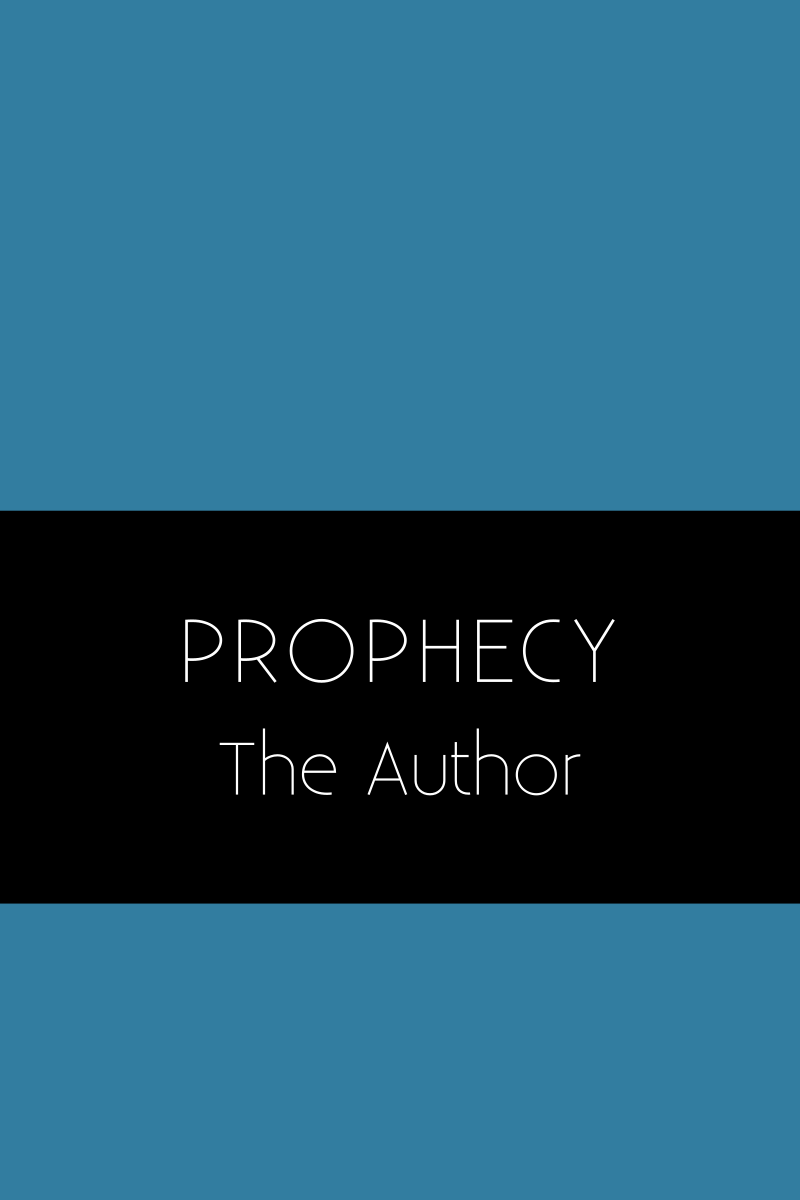
\includegraphics[height=\paperheight]{./desktop-cover.png}}
\fi

\cleartorecto
\thispagestyle{empty}
\vspace*{5em}

{\centering

\settowidth{\titleLength}{%
  {\fontsize{16}{16}\selectfont\ebGaramondSmallCapsFont\textls{Insegnamenti}}%
}

{\fontsize{16}{16}\selectfont\ebGaramondSmallCapsFont\textls{Insegnamenti}}\\[0.3\baselineskip]
\setlength{\xheight}{\heightof{X}}
\raisebox{0.5\xheight}{\color[gray]{0.4}\rule{\titleLength}{0.25pt}}\\[0.3\baselineskip]
{\itshape
\thesubtitle}

\vfill

\theauthor

\vspace*{5em}

}



\cleartoverso
\thispagestyle{empty}

{\copyrightsize
\centering
\setlength{\parindent}{0pt}%
\setlength{\parskip}{0.8\baselineskip}%

\thetitle\ -- \thesubtitle\\
by \theauthor

Published by \thePublisher

ISBN \theISBN

Copyright \copyright\ \thePublisher\ 2017

Cover Photograph: The Person

\vfill

{\footnotesize

This work is licensed under a Creative Commons\\
Attribution-NonCommercial-NoDerivatives 4.0 International~License.

Produced with the \LaTeX\ typesetting system, set in Gentium and Crimson Roman.

\theEditionInfo

}}


\cleartorecto
\thispagestyle{empty}

\mbox{}
\vfill

\begin{quote}
\centering

Per l’aiuto ricevuto nella preparazione di questo libro\\
vogliamo esprimere la nostra gratitudine a molte persone,\\
in particolare al gruppo Kataññutā della Malesia, Singapore e Australia\\
che ne ha reso possibile la stampa.

\end{quote}

\vspace*{4\baselineskip}

\vfill
\mbox{}



\cleartorecto
\tableofcontents*

\chapter{Prefazione}

Gli insegnamenti del venerabile Ajahn Chah tradotti e resi fruibili in
questa edizione sono diretti e chiari. Mi dà molta gioia sapere che una
tale saggezza stia per essere ampiamente diffusa.

Ho avuto la grande fortuna di vivere con Ajahn Chah o di stargli vicino
tra il 1967 e il 1977, gli anni centrali del suo insegnamento. Dopo aver
ricevuto l'ordinazione nel maggio del 1967 nella Thailandia del
nord-est, nella provincia di Nong Khai, il mio precettore mi inviò al
Wat Nong Pah Pong per la formazione. Fu durante il mio primo ritiro
delle piogge (\emph{vassa}) in quel monastero, mentre vivevo sotto la
guida di Ajahn Chah, che davvero crebbero la mia fede e la mia fiducia
nei riguardi di questo modo di praticare. Durante quei dieci anni ho
avuto l'opportunità di studiare e di comprendere la relazione tra il
Dhamma e il Vinaya (la disciplina monastica), di sviluppare una visione
profonda della vacuità e della forma, e di riconoscere la sofferenza
causata dall'ignoranza dei miei attaccamenti ai fenomeni condizionati.

L'approccio di Ajahn Chah all'insegnamento e alla formazione è semplice
e pratico. È uno strumento perfetto per rendere chiare le illusioni del
sé, le presunzioni culturali e sociali nonché i processi del nostro
pensiero. Ora i suoi insegnamenti, originariamente registrati, sono
tradotti, disponibili e facilmente raggiungibili. Sono perciò grato sia
a chi ha lavorato alla traduzione e alla compilazione sia agli sponsor
che hanno reso possibile la distribuzione gratuita.

L'insegnamento del Buddha è un grande dono, ancor più necessario oggi
per far fronte ai problemi delle società contemporanee. Che questa
raccolta di insegnamenti possa essere di beneficio a molte persone.

\bigskip

{\raggedleft
  Luang Por Sumedho,\\
  novembre 2010
\par}

\clearpage

Gli insegnamenti di Ajahn Chah erano disarmanti per la loro immediatezza
e stimolanti per la loro rilevanza. Egli avrebbe detto: «~Se lasciate
andare un po', avrete un po' di pace. Se lasciate andare molto, avrete
molta pace. E se lasciate andare del tutto, avrete una pace totale.~»

Stare vicino a lui significava essere vicino al miglior amico possibile.
Quando eravamo maldestri o sbagliavamo non rideva di noi, rideva con
noi. Quando stavamo soffrendo per i dubbi, non ci rimproverava per
mancanza di fede, ma ci parlava dei tempi in cui lui stesso aveva
dubitato così tanto da pensare che la sua testa sarebbe scoppiata. E se
voleva ispirarci diligenza nella pratica, si sedeva in meditazione con
noi, recitava i canti con noi e lavorava con noi. Il nostro inciampare e
annaspare non erano mai giudicati, ma considerati in un modo che dava
dignità ai nostri sforzi, non disperazione. Gli incoraggiamenti di Ajahn
Chah a lasciar andare non erano né una tecnica né un toccasana; si
trattava piuttosto di condividere la luce che aveva trovato nella sua
pratica, per far sì che anche noi potessimo trovare la direzione verso
la libertà dalla sofferenza.

Osservando la mole di questa edizione, i lettori potrebbero
meravigliarsi del fatto che, sebbene gli insegnamenti fossero stati così
semplici, siano state necessarie così tante parole per esprimerli.
Questo è dovuto al fatto che siamo in grado di generare confusione in
numerosissimi modi. Ajahn Chah conosceva il luogo della pace perfetta ed
era contento di dimorarvi. Egli, però, era anche instancabile nei suoi
sforzi di guidare gli altri. Vivendo con lui, a volte pareva che ci
fosse indicato quel luogo di benessere, un invito a godere i frutti
della pratica. Più spesso era come se lui stesse percorrendo la strada
al nostro fianco.

Come vedrete, questi insegnamenti non sono un manuale di buddhismo. Qui
non troverete neanche le soluzioni a tutti i vostri problemi. Gli
insegnamenti di Ajahn Chah mirano a metterci in contatto con le nostre
domande più profonde e ad aiutarci ad ascoltarle, pazientemente e
gentilmente, fino a quando non si rivela la via da seguire.

I discorsi presenti in questa raccolta sono stati registrati, trascritti
e tradotti molti anni fa e sono in un certo qual modo lontani dalla loro
fonte. Ovviamente, se letti con un cuore ricettivo e con una mente
raccolta, queste ``indicazioni'' verso la Verità forniranno ispirazione
e istruzioni preziose. L'umiltà, la gioia e la saggezza di Ajahn Chah
risplendono nelle sue parole, illuminando il Sentiero mentre lo
percorriamo. Sono trascorsi quasi vent'anni da quando Ajahn Chah è
morto. Grazie al supporto di sponsor generosi, abbiamo colto questa
opportunità di mettere insieme tutti i discorsi disponibili per
distribuzione gratuita e di presentarli in una forma che speriamo possa
essere facilmente accessibile a tutti coloro che si sentono attratti
dalla pace.

\bigskip

{\raggedleft
  Ajahn Munindo,\\
  aprile 2011
\par}


\chapter{Nota ai testi}

\section{Nota al testo inglese}

Questa raccolta di insegnamenti di Ajahn Chah è il risultato della
trascrizione, traduzione e cura redazionale di discorsi originariamente
pronunciati da Ajahn Chah in thailandese o in laotiano. Alcuni di essi
furono impartiti a seguaci laici e molti, forse la maggior parte,
vennero offerti a gruppi monastici, per lo più maschili, che vivevano in
Thailandia con lui.

Alcuni fattori influiscono inevitabilmente non solo sul contenuto, ma
pure sul tono e sull'intensità espressiva degli insegnamenti originari.
Vorrei incoraggiare i lettori a tenere a mente queste circostanze al
fine di apprezzare appieno la portata, l'applicabilità e il senso
complessivo di questi insegnamenti di Dhamma. In un certo senso, man
mano che procedono nella lettura, i laici occidentali dovranno
realizzare una loro propria traduzione interiore, individuando gli
equivalenti per tutte quelle analogie che coinvolgono gli asiatici
bufali d'acqua e il contesto della vita monastico-ascetica nella
foresta; d'altra parte, questo genere di riflessione partecipata --
contemplare come queste parole possano applicarsi alle nostre stesse
vite -- corrisponde esattamente al modo di relazionarsi agli
insegnamenti incoraggiato da Ajahn Chah.

Tra i suddetti fattori, vi sono in primo luogo le difficoltà connesse
alla traduzione dal thailandese, una lingua tonale asiatica
profondamente influenzata dal buddhismo, a una lingua europea con le sue
eredità culturali. Per di più, diversi traduttori hanno lavorato agli
insegnamenti raccolti in questo volume. Le differenti nazionalità e
formazioni di questi traduttori comportano inevitabilmente delle
variazioni nel tono, nello stile e nel vocabolario dei vari capitoli.

In secondo luogo, in Occidente la cultura buddhista è molto cambiata nel
trentennio durante il quale sono state effettuate le traduzioni. Mentre
in precedenza i traduttori hanno forse pensato che molti concetti
buddhisti necessitassero di essere trasposti in termini più familiari
agli occidentali, oggi vi è una maggiore consapevolezza della visione
buddhista del mondo; ad esempio, termini quali ``kamma'' e ``Nibbāna''
fanno ora parte del vocabolario inglese. I discorsi raccolti in questo
volume manifestano perciò un'ampia gamma di modi di tradurre termini e
concetti buddhisti.

In terzo luogo, il contesto monastico buddhista implicava che termini
thailandesi e in lingua pāli con significato tecnico costituissero una
parte consueta e accettata dello stile d'insegnamento vernacolare. I
diversi traduttori hanno preso varie decisioni a proposito di come
rendere tali termini tecnici. Ad esempio, nella lingua thailandese la
stessa parola può significare sia ``cuore'' che ``mente'', e i
traduttori sono stati costretti a scegliere. I lettori dovrebbero
rammentarlo qualora incontrino termini utilizzati in modi che a loro
sembrano non del tutto consueti o non coerenti in un discorso rispetto a
un altro. Spesso alcuni termini sono spiegati nel contesto o con una
nota al testo e, in aggiunta, in un \emph{Glossario} che può essere
rintracciato alla fine del libro.

Confidiamo di essere riusciti, con i nostri sforzi, a restituire in
forma scritta istruzioni orali senza oscurare le intenzioni del maestro.
È stato inevitabile ricorrere ad alcuni compromessi, perché diversi sono
stati i traduttori che hanno cercato di trovare un equilibrio fra
traduzione letterale e traduzione libera. Per questa compilazione
abbiamo revisionato alcune delle traduzioni al fine di standardizzare
termini e stile. Ci siamo ovviamente attenuti al minimo indispensabile.
Ulteriori edizioni di questi scritti potrebbero mirare a un più alto
grado di standardizzazione.

Infine, soprattutto nella terza parte, \emph{Pratica della rinuncia}, i
discorsi di Ajahn Chah furono pronunciati in un contesto nel quale
l'uditorio era per lo più impegnato nella vita celibataria di rinuncia.
Questa circostanza inevitabilmente dà un colore netto al modo in cui il
Dhamma viene presentato. Inoltre, Ajahn Chah parlò molto spesso solo a
uomini. Tale fatto spiega il costante uso di pronomi esclusivamente
maschili in molti di questi discorsi; anche se ad alcuni il fatto che un
tal genere di linguaggio sia stato lasciato intatto può apparire un
ostacolo, a noi è parso inopportuno prenderci la libertà di eliminarlo.
Così, ai lettori potrà talvolta essere di nuovo necessario ricorrere a
traduzioni interiori oppure o all'immaginazione, affinché si palesi
l'importanza di quegli insegnamenti per la loro stessa vita.

Ajahn Chah insegnò ai monaci riuniti in piccole \emph{sālā} in legno
debolmente illuminate da lampade a cherosene. Gli insegnamenti spesso
avevano la forma di esortazioni offerte al termine della recitazione del
\emph{Pāṭimokkha}, il codice di disciplina monastica, che ha luogo ogni
due settimane. Questi insegnamenti erano espressamente rivolti ai monaci
residenti, e per questo i lettori laici dovrebbero ricordare di trovarsi
al cospetto sia di una pratica di rinuncia buddhista sia di un insieme
di insegnamenti di Dhamma. I tre titoli \emph{Pratica quotidiana},
\emph{Pratica formale} e \emph{Pratica della rinuncia} utilizzati per
organizzare questi discorsi non devono essere presi troppo alla lettera.
In ciascun discorso sono presenti sovrapposizioni e, di conseguenza, non
è necessario che ognuno di essi sia letto nell'ordine in cui è stato
presentato.

La preparazione e la presentazione di questa compilazione è il frutto
del lavoro di un gruppo che si è avvalso del tempo e dell'abilità di
numerosi lettori di bozze, tecnici e grafici. Una menzione particolare
meritano i contributi di due dei traduttori originari, Paul Breiter e
Bruce Evans. Siamo debitori verso tutti coloro che hanno contribuito con
il loro tempo e il loro impegno a condurre a completamento questo
progetto.

Speriamo sinceramente che, con queste prospettive nel cuore, le parole
contenute in questo volume siano utili a ogni lettore e possano essere
una condizione per la realizzazione del Nibbāna. Fu con la stessa
intenzione che Ajahn Chah parlò per tanti anni. Che queste intenzioni
possano maturare nella vita del lettore e condurlo alla pace e alla
libertà complete.

\bigskip

{\raggedleft
  I compilatori
\par}

\section{Nota al testo italiano}

È opportuno illustrare sia i criteri soggiacenti alla traduzione
dall'inglese all'italiano sia qualche scelta redazionale. Nel testo
degli \emph{Insegnamenti} di Ajahn Chah gli interventi sono rarissimi:
sono stati ritenuti necessari solo quando inevitabili per aiutare il
lettore nella comprensione. D'altra parte, nella traduzione sono state
di proposito utilizzate le parole più semplici, per evitare che i testi
avessero un tono ricercato o intellettualistico. Sono state lasciate
spesso inalterate le ripetizioni di concetti e di parole, connesse al
tenore orale dell'esposizione. Di tanto in tanto la punteggiatura è
stata ritoccata, e talora è stato aggiunto o eliminato qualche
capoverso.

Per molti dei discorsi presenti negli \emph{Insegnamenti}, ai differenti
traduttori dal thailandese all'inglese si sono in passato sovrapposti
vari traduttori italiani che hanno lavorato sui testi in inglese. Questa
traduzione, effettuata da una sola persona ma con la collaborazione di
altre, è stata realizzata del tutto indipendentemente dalle precedenti
traduzioni italiane al fine di uniformare -- come auspicato pure nella
\emph{Nota al testo} dell'edizione inglese -- le variazioni di stile e
di vocabolario.

In apertura sono state tradotte entrambe le \emph{Prefazioni}, sia
quella di Ajahn Sumedho, presente nell'edizione in tre volumi, sia
l'altra di Ajahn Munindo, disponibile invece nell'edizione in volume
unico\emph{.} L'\emph{Introduzione} di Ajahn Amaro è tradotta dal testo
ampliato, rivisto dallo stesso autore e pubblicato successivamente a
parte con il titolo \emph{An Introduction to the Life and Teachings of
Ajahn Chah} (Amaravati Publications 2012).

Negli \emph{Insegnamenti} i termini in lingua pāli sono stati resi in
corsivo -- ad eccezione di ``Buddha'', ``Dhamma'', ``Saṅgha'',
``Vinaya'', ``Nibbāna'' e ``kamma'', che invece sono in tondo -- e compaiono nella forma tematica
oppure al nominativo singolare o plurale, in base al contesto. Questi
termini, insieme ad altri concetti di rilievo, sono brevemente spiegati
alla fine del volume, nel \emph{Glossario}, e nelle note a pié di
pagina, che da quest'ultimo sono per lo più riprese. Sia nel
\emph{Glossario} sia nelle note predomina invece la forma tematica, un
fatto che spiega alcune difformità tra il testo e le note. Per quanto
concerne il \emph{Glossario}, in qualche caso si è ritenuto necessario
ampliare qualche voce e aggiungerne altre.

Fra i tanti che hanno contribuito a questa edizione italiana, i lettori
siano grati anche a bhikkhu Mahāpañño, che ha rivisto il testo con
grande accuratezza, a Mario Bracchetti e a Sara Bellettato, che hanno
contribuito alla revisione e, infine, ad Antonella Serena Comba, che ha
collaborato alla stesura del \emph{Glossario}.



\chapter{Introduzione}



\textbf{Una sera nel nord-est della Thailandia}

La notte sta scendendo rapidamente. La foresta risuona dell'ondoso
brusio di innumerevoli grilli e dell'inquietante e crescente gemito
delle cicale tropicali. Poche stelle si intrufolano fiocamente tra le
cime degli alberi. Nella crescente oscurità, un paio di lanterne a
cherosene producono una pozza di caldo chiarore, illuminando l'area
all'aperto sottostante una capanna issata su pali di legno. Sotto il
bagliore, due dozzine di persone sono raccolte attorno a un monaco,
piccolo ma di solida costituzione, che siede a gambe incrociate su una
grande sedia di vimini. Una pace vibrante è nell'aria. Il venerabile
Ajahn Chah sta insegnando.

Il gruppo riunito è per alcuni aspetti eterogeneo. Accanto ad Ajahn Chah
-- o Luang Por,\footnote{~Luang Por (in thailandese หลวงพ่อ).
  ``Venerabile padre''; è un'espressione che viene utilizzata in
  Thailandia per rivolgersi ai monaci anziani.} venerabile padre, come è
affettuosamente chiamato dai suoi allievi -- vi sono i \emph{bhikkhu},
ossia i monaci, e i novizi. La maggior parte di loro è thailandese o
laotiana, ma ve ne sono alcuni dalla pelle chiara: un canadese, due
statunitensi, un giovane australiano e un inglese. Di fronte ad Ajahn
Chah siede una ben curata coppia di mezz'età, lui in giacca e pantaloni
e lei ingioiellata e acconciata alla moda; stanno cogliendo
l'opportunità -- lui è un membro del Parlamento thailandese e proviene
da una lontana provincia, e ora si trova in zona per questioni ufficiali
-- per venire a porgere i loro omaggi a Luang Por e per fare offerte al
monastero.

Un po' più indietro, da entrambi i lati, è sparso un consistente gruppo
di persone che abitano nei villaggi dei dintorni. Le magliette e le
bluse che indossano sono usurate e la pelle delle loro magre membra è
scura e bruciata dal sole, aggrinzita, cotta come la povera terra di
questa regione. Luang Por, da bambino, con alcuni di loro aveva giocato,
aveva catturato rane e si era arrampicato sugli alberi; altri li aveva
aiutati -- ed era stato da loro aiutato -- prima di diventare
\emph{bhikkhu} quando arrivava l'annuale turno di piantare il riso e poi
di mieterlo nei campi alla fine del monsone.

Da un lato, nei pressi del retro, c'è una professoressa di Friburgo,
giunta in Thailandia per studiare il buddhismo con un'amica del suo
gruppo di Dhamma; una monaca statunitense della sezione femminile del
monastero è venuta con lei per guidarla tra i sentieri della foresta e
per farle da traduttrice. Accanto a loro siedono tre o quattro altre
monache più anziane del monastero, che hanno deciso di cogliere
l'opportunità per venire a chiedere consiglio a Luang Por su un problema
della comunità femminile e per domandargli di visitare -- sono già
passati molti giorni dall'ultima volta che lo ha fatto -- il lato della
foresta nel quale dimorano e di offrire un discorso di Dhamma al loro
gruppo. Sono rimaste già per un paio d'ore e perciò, dopo aver prestato
omaggio, hanno preso congedo insieme alle altre visitatrici provenienti
dalla sezione monastica femminile: devono tornare prima che sia buio e
sono già un po' in ritardo.

Sempre nei pressi del retro, quasi sul limitare della pozza di luce,
siede con il volto severo un uomo sulla trentina. Per metà è girato di
lato, come se si senta a disagio e quasi che la sua presenza sia
provvisoria. È un ``duro'' del luogo, un \emph{nak leng}.\footnote{In
  thailandese นักเลง.} Profondamente sprezzante nei riguardi di tutto
quanto possa essere religioso, seppur a denti stretti nutre tuttavia per
Luang Por un rispetto che nasce sia dalla reputazione di
imperturbabilità, forza e resistenza dell'\emph{ajahn} sia dal fatto che
se i fedeli si recano da lui è perché si tratta di una persona genuina.
«~Nell'intera provincia, è probabilmente l'unico cui valga la pena di
prostrarsi.~»

È arrabbiato e sconvolto. È infelice. Una settimana prima, il suo amato
fratello minore, che faceva parte della sua banda e insieme al quale
aveva superato mille difficoltà, s'è ammalato di malaria cerebrale e, in
pochi giorni, è morto. Da allora è come se una lancia gli avesse
trafitto il cuore e nulla al mondo ha più senso, o sapore. «~Se fosse
stato accoltellato, almeno lo avrei potuto vendicare. Che posso fare?
Rintracciare la zanzara che lo ha punto e ucciderla?~» Un amico gli ha
detto: «~Perché non vai a trovare Luang Por Chah?~» Così, eccolo qui.

Quando Luang Por giunge a un punto importante del suo discorso fa un
ampio sorriso e alza un bicchiere per illustrare la sua analogia. Ha
notato la rigida e desolata figura del giovane nell'ombra. Come se
stesse riavvolgendo il filo di una canna da pesca per catturare un pesce
forte e scaltro, presto riesce in un qualche modo a convincerlo a venire
in prima fila. Subito dopo, il \emph{nak leng} piange come un bambino,
mentre Luang Por gli tiene la testa fra le mani. L'uomo ride della sua
stessa arroganza e auto-ossessione, e capisce di non essere stato il
primo o il solo ad avere perso una persona cara: le lacrime di rabbia e
dolore si sono trasformate in lacrime di sollievo.

Tutto ciò avviene alla presenza di venti estranei, e ora l'atmosfera è
di sicurezza e fiducia. Perché sebbene le persone qui riunite provengano
da differenti ceti sociali e da diverse parti del mondo, sono tutte
accomunate in questo momento e in questo luogo dall'essere
\emph{saha-dhammika}, ``compagni di viaggio nel Dhamma'' o, per usare
un'altra espressione vernacolare buddhista, ``tutti fratelli e sorelle
nella vecchiaia, malattia e morte'', e appartengono perciò alla stessa
famiglia.

Questo genere di situazioni si verificò innumerevoli volte durante i
trent'anni d'insegnamento di Ajahn Chah. È significativo che sia nelle
più lunghe esposizioni legate a occasioni formali sia in dialoghi di tal
genere, all'impronta, il fluire dell'insegnamento e la scelta di coloro
ai quali esso doveva essere specificamente indirizzato fossero del tutto
spontanei e imprevedibili. Per molti aspetti, quando Ajahn Chah
insegnava era come un maestro musicista che guida il flusso dell'armonia
e la produce in assoluta aderenza alle caratteristiche e agli stati
d'animo delle persone con le quali si trova. Integrava le loro parole,
sentimenti e interrogativi nel crogiolo del suo cuore e lasciava che le
risposte sgorgassero liberamente.

Quale che fosse il tipo di persone che si raccoglieva attorno a lui, con
identica impassibilità poteva usare come esempio i modi giusto e
sbagliato di sbucciare un mango e, subito dopo, descrivere la natura
della Realtà Ultima. Poteva essere burbero e freddo con le persone
tronfie e, il momento successivo, incantevole e gentile con quelle
timide; oppure, raccontare una barzelletta con un vecchio amico del
villaggio e, poi, guardare negli occhi un corrotto colonnello di polizia
e parlargli con sincerità della centrale importanza dell'onestà nel
Sentiero del Buddha. Poteva rimproverare un \emph{bhikkhu} perché
indossava l'abito in modo sciatto e poi, nel volgere di pochi minuti,
lasciare che la sua stessa veste, scivolatagli dalla spalla, scoprisse
la sua pancia tonda.

Una domanda intelligente posta da un accademico alla ricerca di
discussioni filosofiche di alto livello per mostrare il suo acume,
facilmente induceva Luang Por a rimuoversi la dentiera e a passarla
all'assistente \emph{bhikkhu} affinché gli desse una pulita.
L'interlocutore avrebbe così dovuto superare la prova: il grande maestro
rispondeva al suo profondo quesito con le ampie labbra ripiegate
all'indietro, sulle gengive, prima che la dentiera, ripulita, fosse
rimessa al suo posto~...

La maggior parte delle volte Ajahn Chah impartiva i suoi insegnamenti in
riunioni spontanee, ma offriva molto generosamente la sua saggezza anche
in occasioni più formali, come dopo la recitazione delle regole per i
\emph{bhikkhu}, oppure all'intera assemblea di laici e monaci nella
notte di settimanale osservanza lunare. Ovviamente, sia che si trattasse
di insegnamenti per il primo o per il secondo tipo di riunioni, Ajahn
Chah non pianificava mai nulla. Non una sola sillaba di ciò che
insegnava era annotata prima di iniziare a parlare. Pensava che questo
fosse un principio estremamente importante, perché il compito
dell'insegnante consisteva nel togliersi di mezzo, e lasciare che il
Dhamma sorgesse in accordo con le necessità del momento. Diceva: «~Se
non è vivo nel presente, non è Dhamma.~»

Una volta invitò il suo primo discepolo occidentale, Ajahn Sumedho, a
tenere un discorso all'assemblea di monaci e di laici del monastero
principale, il Wat Pah Pong. Fu una prova traumatizzante: si trattava
non solo di parlare a circa duecento persone abituate all'alto standard
di arguzia e di saggezza di Ajahn Chah, ma per di più in thailandese,
una lingua che Ajahn Sumedho aveva iniziato a imparare solo tre o
quattro anni prima. Nella sua mente si affollarono idee e paure. In quei
giorni stava leggendo testi riguardanti i Sei Regni della cosmologia
buddhista e i correlati stati psicologici: l'ira e i regni infernali, la
felicità sensoriale e i regni paradisiaci, e così via. Decise che
sarebbe stato un buon argomento e pensò al modo opportuno di esprimere
tutte le sue idee.

Quando giunse la notte fatidica, Ajahn Sumedho tenne il suo discorso e
ritenne che fosse andata piuttosto bene. Il giorno seguente molti membri
del Saṅgha si recarono da lui per dirgli quanto avessero apprezzato le
sue parole. Si sentì sollevato e abbastanza soddisfatto di se stesso. Un
po' di tempo dopo, in un momento di tranquillità, Ajahn Chah catturò la
sua attenzione, lo fissò negli occhi e gli disse con gentilezza: «~Non
farlo mai più.~» Questo modo di insegnare non era tipico solo di Ajahn
Chah, ma era adottato da tutta la cosiddetta Tradizione Thailandese
della Foresta. Perciò, può essere utile descrivere le caratteristiche e
le origini di questo lignaggio, per mostrare un po' il significato del
contesto dal quale scaturì la saggezza di Ajahn Chah.

\textbf{La Tradizione della Foresta}

In relazione alla meditazione, la Tradizione della Foresta è in un certo
qual senso addirittura precedente al Buddha. Prima dei suoi tempi, in
India e nella regione dell'Himalaya, non era inconsueto per coloro che
cercavano la liberazione spirituale abbandonare la vita delle città e
dei villaggi per recarsi nella natura incontaminata di montagne e
foreste. In quanto gesto per lasciarsi alle spalle i valori del mondo,
ciò recava in sé un senso perfettamente compiuto: la foresta era un
posto selvaggio e naturale, e lì si potevano incontrare solo criminali,
folli, emarginati e rinuncianti sulla via della spiritualità. Si
trattava di un ambiente estraneo all'influsso delle regole culturali
materialistiche, quindi ideale alla coltivazione degli aspetti
spirituali che le trascendevano.

Quando all'età di 29 anni il \emph{bodhisatta}\footnote{\emph{bodhisatta}.
  Un essere che si impegna per raggiungere il Risveglio.} abbandonò la
vita del palazzo, lo fece per trasferirsi nella foresta e addestrarsi
nelle discipline yoga praticate in quel tempo. La storia di come Egli,
insoddisfatto dagli insegnamenti dei suoi primi istruttori, li lasciò
per cercare la sua propria strada per la Liberazione è nota. Vi riuscì,
scoprendo all'ombra dell'albero della bodhi, sulla riva del fiume
Nerañjara, nel luogo ora chiamato Bodh-Gaya nello stato del Bihar in
India, quel primario fondamento della Verità che chiamò ``la Via di
Mezzo''.

Spesso si afferma che il Buddha nacque in una foresta, ottenne
l'Illuminazione in una foresta, visse e insegnò per tutta la vita in una
foresta e, infine, morì in una foresta. Quando gli era possibile
scegliere, era l'ambiente che preferiva perché, come Egli diceva: «~I
\emph{Tathāgata}\footnote{\emph{Tathāgata}. Letteralmente, ``così
  andato'', ``così venuto''.} provano diletto nei luoghi isolati.~» Il
lignaggio ora conosciuto come Tradizione Thailandese della Foresta cerca
di vivere nello spirito della via abbracciata dal Buddha stesso, e di
praticare in accordo con gli stessi criteri da Lui incoraggiati durante
la sua vita. Si tratta di un ramo della Scuola Meridionale del
Buddhismo, più comunemente denominato ``Theravāda''.

Secondo quanto ci dicono le pur approssimative narrazioni storiche,
pochi mesi dopo la morte del Buddha fu tenuto un grande concilio di
anziani per stabilire e formalizzare gli Insegnamenti -- i discorsi e le
regole monastiche -- in una vernacolare forma standardizzata detta
\emph{pālibhasa}, ``il linguaggio dei testi''. Gli insegnamenti di
Dhamma formulati in tal modo durante il secolo successivo formano il
nucleo del Canone in lingua pāli, la base comune per varie scuole
buddhiste successive. Cento anni dopo fu tenuto un secondo concilio che,
per tentare di mettere tutti d'accordo, tornò nuovamente su tutti gli
Insegnamenti.

Ovviamente fu proprio allora che, come si è scoperto, avvenne il più
rilevante scisma nel Saṅgha. La maggioranza volle modificare alcune
delle regole, anche permettendo ai monaci di usare il denaro. In
relazione ai cambiamenti proposti, un piccolo gruppo fu cauto e pensò:
«~Bene, che abbia senso o meno, vogliamo fare le cose nel modo in cui le
fecero il Buddha e i suoi primi discepoli.~» I suoi membri sono
conosciuti in sanscrito come \emph{sthavira} e in pāli come
\emph{thera}, ``anziani''. Dopo centotrenta anni circa, diedero origine
alla Scuola del Theravāda. ``Theravāda'', che significa letteralmente
``la Via degli Anziani'', da allora ha proprio questa caratteristica
costante. L'etica della tradizione può essere racchiusa nella frase
``nel bene e nel male, questa è la via fissata dal Buddha, e così noi
faremo''. Perciò, può essere riscontrato da sempre in essa un tratto
particolarmente ``conservatore''.

Com'è avvenuto per tutte le tradizioni religiose e le istituzioni
dell'uomo, col trascorrere del tempo numerosi furono i rami che
germogliarono dalla radice del Buddha. È stato detto che circa 250 anni
dopo di Lui, durante l'impero di Asoka, vi furono fino a diciotto scuole
e lignaggi in India, e forse più, con divergenti modi di vedere il
\emph{Buddha-sāsana}, la dottrina del Buddha. Un lignaggio si stabilì
nello Sri Lanka, a una certa distanza dal fermento culturale dell'India,
dove giungevano influssi religiosi dall'Occidente e dall'Oriente e
andava contestualmente verificandosi un risveglio del brahmanesimo che
si aggiungeva all'agitarsi di nuove forme del pensiero buddhista. Tale
lignaggio si sviluppò per conto proprio, e fu meno soggetto a influssi e
stimoli. Formulò i propri commenti e interpretazioni delle Scritture in
lingua pāli senza l'intenzione di sviluppare nuove forme che
rispecchiassero sollecitazioni provenienti da altre fedi, ma con lo
scopo di aggiungere alcuni dettagli. Alcuni di essi avevano
caratteristiche fiabesche, miranti a catturare il cuore della gente
comune, altri erano più filosofici e metafisici, di genere erudito.

Anche il buddhismo \emph{theravādin} tuttavia si cristallizzò.
Nonostante guerre, carestie e altri rivolgimenti culturali del
subcontinente indiano, il Theravāda è sopravvissuto fino ai nostri
giorni, soprattutto perché si consolidò originariamente nell'isola di
Sri Lanka, un rifugio più sicuro di molti altri. Anche altre furono le
scuole buddhiste che qui operarono, ma il buddhismo \emph{theravādin} fu
continuamente rigenerato e conservato quale principale religione
dell'isola.

Questo lignaggio si diffuse infine, in tempi differenti, in tutto il
sud-est asiatico, allorché furono invitati missionari dallo Sri Lanka e
dall'India. Raggiunse la Birmania e in seguito la Thailandia, la
Cambogia e il Laos e, da ultimo, arrivò da tali territori pure in
Occidente. Durante questa diffusione geografica della tradizione
\emph{theravādin}, si continuò a guardare al Canone in pāli come
normativo. Quando il lignaggio si stabilì in nuovi paesi, vi fu sempre
un forte senso di deferenza e venerazione per gli insegnamenti
originali, come pure rispetto per lo stile di vita incarnato dal Buddha
e dal Saṅgha originario, i monaci dei primi tempi che dimoravano nella
foresta.

Tale modello, utilizzato in quegli anni e da allora in poi impiegato per
così tanti secoli, ebbe ovviamente un gran numero di momenti sia propizi
sia sfavorevoli. Talora la religione si affievolì nello Sri Lanka e
allora, per rivitalizzarla, vi arrivarono monaci dalla Thailandia.
Quando poi ebbe la tendenza a smorzarsi in quest'ultimo territorio,
furono monaci provenienti dalla Birmania a rafforzarla. I seguaci del
Theravāda si supportarono vicendevolmente nei secoli e, così, questa
tradizione riuscì a mantenersi a galla per larga misura nella sua forma
originale.

Assieme alla degenerazione, un altro aspetto problematico di questi
cicli fu il successo. Quando la religione si sviluppò bene, spesso i
monasteri si arricchirono e l'intero sistema si corruppe, divenne
``obeso'' e iniziò a collassare sotto il suo stesso peso. Si verificava
allora la scissione di un gruppo che -- affermando: «~Torniamo alle cose
essenziali~» -- si allontanava nella foresta e tornava di nuovo ai
modelli originari, mantenendo i precetti monastici, praticando la
meditazione e studiando gli insegnamenti originari.

È significativo notare che questo ciclo di progresso, enfiagione,
corruzione e riforma si sia verificato numerose volte nel corso dei
secoli in molte altre nazioni buddhiste. È impressionante quanto le vite
e la pratica di luminari quali il venerabile Patrul Rimpoche nel Tibet e
il venerabile maestro Xu Yun in Cina -- entrambi della fine del XIX e
degli inizi del XX secolo -- siano in completo accordo con lo spirito
della Tradizione della Foresta. Entrambi scelsero di vivere in grande
semplicità, osservarono la disciplina monastica molto rigorosamente,
furono esperti meditanti e maestri molto dotati. Evitarono in larga
misura gli oneri gerarchici e responsabilità ufficiali, ma
inevitabilmente ascesero a posizioni di grande influenza mediante il
potere puro della saggezza e della virtù. Questo è esattamente il
modello di vita incarnato anche dai grandi maestri della Tradizione
Thailandese della Foresta.

Intorno alla metà del XIX secolo, il buddhismo in Thailandia era
caratterizzato da una ricca varietà di pratiche e tradizioni regionali,
ma lo standard generale della vita spirituale si era in certo qual modo
corrotto, la disciplina monastica si era rilassata e gli insegnamenti di
Dhamma erano fusi con caotici elementi tantrici e animistici, senza
contare il fatto che quasi nessuno praticava più la meditazione. Inoltre
-- e forse proprio questa è la cosa più importante -- la posizione
ortodossa, rappresentata da studiosi e non solo da monaci negligenti,
poco colti o confusi, affermava che non era possibile ai nostri giorni
realizzare il \emph{Nibbāna} e nemmeno conseguire i \emph{jhāna}, i vari
livelli di assorbimento meditativo. I rianimatori della Tradizione della
Foresta rifiutavano di accettarlo. Era anche una delle ragioni per cui
erano considerati dalla gerarchia ecclesiastica di quegli anni alla
stregua di dissidenti e piantagrane, mentre molti di loro, compreso
Ajahn Chah, erano conseguentemente disprezzati -- lo era anche il loro
ritornello: «~Non otterrai la saggezza dai libri~» -- dalla maggior
parte dei monaci eruditi del loro stesso lignaggio \emph{theravādin}.

È necessario precisare questo punto, per evitare che induca perplessità
il fatto che Ajahn Chah possa aver avuto un'attitudine tanto negativa
nei riguardi dello studio, soprattutto perché, in quanto appartenente
alla tradizione \emph{theravādin}, si suppone che egli dovesse invece
nutrire grande venerazione per la parola del Buddha. È in questione un
motivo cruciale, che caratterizza i monaci appartenenti alla Tradizione
della Foresta: la determinazione a focalizzare l'attenzione sullo stile
di vita e sull'esperienza personale, piuttosto che sui libri e
soprattutto sui Commenti al Canone in pāli. Si potrebbe pensare che una
tale attitudine possa essere presuntuosa e arrogante, o un'espressione
di gelosia di una mente poco colta per altre migliori: non è così, se si
riesce a comprendere che proprio le interpretazioni degli studiosi
stavano trascinando il buddhismo in un abisso. In poche parole, era
proprio il tipo di situazione a rendere il panorama spirituale maturo
per il rinnovamento: fu da questo fertile terreno che emerse la
rinascita della Tradizione della Foresta.

La Tradizione Thailandese della Foresta non sarebbe così com'è oggi se
non vi fosse stato l'influsso di un grande maestro in particolare. Si
tratta del Venerabile Ajahn Mun\footnote{Nella traduzione si è scelto di
  lasciare ``Mun'', come di solito si rinviene nei testi inglesi. Si
  avverte il lettore italiano che, però, l'esatta pronuncia thailandese
  è ``Màn''.} Bhuridatta. Nacque nel 1870 nella provincia di Ubon, dove
la Thailandia s'incontra con il Laos e la Cambogia. Allora era, e lo è
ancora, una delle zone più povere del paese, ma pure quella in cui la
durezza della terra e il carattere affabile delle persone hanno indotto
nel mondo una spiritualità di rara profondità.

Ajahn Mun era un giovane di mente vivace. Eccelleva nel \emph{mor
lam},\footnote{In thailandese หมอลำ.} l'arte locale di comporre canzoni
popolari in versi, ed era anche fortemente attratto dalla pratica
spirituale. Subito dopo l'ordinazione a \emph{bhikkhu}, cercò il
Venerabile Ajahn Sao, uno dei rari monaci della foresta del luogo, e gli
chiese di insegnargli la meditazione. Si era pure reso conto del fatto
che una rigorosa adesione alla disciplina monastica sarebbe stata
fondamentale per i suoi progressi spirituali. Divenne discepolo di Ajahn
Sao e si dedicò alla pratica con grande vigore.

Se oggi, dal nostro punto di vista, queste due cose -- disciplina
rigorosa e meditazione -- potrebbero sembrarci scontate, allora la
disciplina era diventata piuttosto trasandata in tutta la regione e la
meditazione era considerata con grande sospetto. Probabilmente solo chi
era interessato alla magia nera era abbastanza folle per avvicinarsi
alla meditazione, e si riteneva probabile che essa conducesse alla
pazzia o causasse possessioni spiritiche.

Col tempo Ajahn Mun riuscì a spiegare con successo e a dimostrare
l'utilità della meditazione a molte persone, e divenne anche un esempio
di un più alto standard di vita per la comunità monastica. Inoltre egli
divenne il più considerato maestro spirituale della Thailandia,
nonostante il fatto che vivesse in luoghi remoti. Quasi tutti i più
esperti e venerati maestri di meditazione thailandesi del XX secolo
furono o suoi diretti discepoli o ne subirono profondamente l'influsso.
Tra essi, Ajahn Chah.

\textbf{Ajahn Chah}

Ajahn Chah nacque in una famiglia grande e agiata, in un villaggio della
Thailandia nord-orientale. Dietro sua stessa iniziativa, alla tenera età
di nove anni scelse di lasciare la casa paterna e andò a vivere nel
monastero del luogo. Fu ordinato novizio e, sentendo il richiamo della
vita religiosa, a vent'anni ricevette l'ordinazione completa. In quanto
giovane \emph{bhikkhu}, studiò i fondamenti del Dhamma, la disciplina e
altre scritture.

In seguito, insoddisfatto del blando standard di vita nel tempio del suo
villaggio, e desiderando una guida nella meditazione, abbandonò questi
luoghi piuttosto sicuri e intraprese la vita del \emph{bhikkhu} errante,
in continuo \emph{tudong}.\footnote{\emph{tudong} (in thailandese
  ธุดงค์). La pratica ascetica di errare a piedi, nelle campagne, in
  pellegrinaggio o alla ricerca di posti tranquilli per ritiri solitari,
  vivendo di cibo offerto in elemosina.} Cercò vari maestri locali di
meditazione e praticò sotto la loro guida. Peregrinò per un certo numero
di anni come fanno i \emph{bhikkhu} che seguono le pratiche ascetiche,
dormendo in foreste, caverne e luoghi di cremazione, e trascorse un
breve ma illuminante periodo con lo stesso Ajahn Mun. Questa è la
descrizione di quell'incontro altamente significativo, tratta
dall'ancora inedita biografia di Luang Por Chah, \emph{Uppalamani} -- un
gioco di parole che significa sia ``Il gioiello della provincia di
Ubon'' sia ``Il gioiello nel loto'' -- scritta da Phra Ong
Neung.\footnote{La biografia di Ajahn Chah è nel frattempo stata
  pubblicata in thailandese ed è anche stata tradotta in inglese con il
  titolo \emph{Stillness Flowing. The Life and Teachings of Ajahn Chah}
  (Panyaprateep Foundation 2017); la traduzione italiana è in corso.}

\begin{quote}
Alla fine del Ritiro delle Piogge,\footnote{L'annuale periodo di tempo
  di tre mesi, che in India corrisponde a quello dei primi tre mesi
  monsonici, durante i quali i monaci hanno la regola dell'obbligo di
  residenza in monastero, un periodo che tradizionalmente è dedicato a
  una formazione più intensiva.} insieme ad altri tre monaci, un novizio
e due laici, Ajahn Chah si incamminò per tornare nell'Isan, il nord-est
della Thailandia. Interruppero il viaggio a Bahn Gor e, dopo pochi
giorni di riposo, iniziò la lunga escursione di 250 chilometri verso
nord. Il decimo giorno raggiunsero l'elegante \emph{stūpa} bianco di
That Phanom, un antico luogo di pellegrinaggio sulle rive del Mekong, e
prestarono omaggio alle reliquie del Buddha lì custodite. Continuarono
il loro itinerario per tappe, cercando monasteri della foresta ubicati
lungo il cammino, nei quali trascorrere la notte. Anche così era un
viaggio arduo, e il novizio e un laico chiesero di tornare indietro.
Quando finalmente arrivarono al Wat Peu Nong Nahny, ove dimorava il
Venerabile Ajahn Mun, il gruppo si era ridotto a soli tre monaci e un
laico.

Allorché entrarono nel monastero, Ajahn Chah fu immediatamente colpito
dall'atmosfera serena e appartata. L'area centrale, nella quale si
trovava una piccola \emph{sālā}, un luogo di ritrovo in legno, era
perfettamente ramazzata, immacolata, e i pochi monaci che furono in
grado di vedere erano silenziosamente intenti a svolgere, con grazia
misurata e composta, le loro faccende quotidiane. C'era un qualcosa nel
monastero che lo rendeva diverso da tutti gli altri nei quali era stato
prima di allora: il silenzio era stranamente denso e vibrante. Ajahn
Chah e i suoi compagni furono accolti educatamente e, dopo essere stati
informati su dove avrebbero dovuto lasciare i loro
\emph{glot},\footnote{~\emph{glot} (in thailandese กลค). Ombrello con
  una zanzariera tutt'intorno all'estremità, utilizzato sia per la
  meditazione sia come riparo dai monaci che intraprendono il
  \emph{tudong}; viene appeso ai rami degli alberi così da potercisi
  sedere sotto, al riparo dagli insetti.} fecero un bagno di benvenuto
per ripulirsi dalla sporcizia del viaggio.

Verso sera, i tre giovani monaci, con il \emph{saṅghāti}\footnote{~\emph{saṅghāti},
  in thailandese \emph{sanghati} (สังฆาฏ). La veste esterna a doppio
  strato che costituisce, assieme alla veste superiore e inferiore,
  l'abito completo da monaco; generalmente viene portata ripiegata lungo
  la spalla sinistra in situazioni cerimoniali.} ordinatamente ripiegato
sulla loro spalla sinistra e con il cuore che oscillava tra appassionata
attesa e freddo timore, si incamminarono verso la \emph{sālā} per
rendere omaggio ad Ajahn Mun. Avanzando lentamente sulle ginocchia verso
il grande maestro, affiancato da entrambi i lati dai \emph{bhikkhu} del
monastero, Ajahn Chah avvicinò una figura anziana ed esile, di presenza
invincibilmente adamantina. È facile immaginare gli occhi senza fondo di
Ajahn Mun, mentre con il suo sguardo penetrante forava Ajahn Chah,
prostratosi per tre volte e poi sedutosi più in basso a conveniente
distanza. La maggior parte dei monaci era seduta in meditazione, a occhi
chiusi; uno sedeva dietro Ajahn Mun, a poca distanza, e con un ventaglio
allontanava dolcemente da lui le zanzare della sera.

Alzando lo sguardo, Ajahn Chah notò sia la clavicola di Ajahn Mun, che
prominente al di sopra dell'abito sporgeva attraverso il pallido
incarnato, sia le sue labbra sottili che, tinte di rosso dal succo di
betel, erano in forte contrasto con la strana luminosità della sua
presenza. Seguendo un'usanza da tempo onorata tra i monaci buddhisti,
inizialmente Ajahn Mun chiese ai visitatori da quanto tempo indossavano
l'abito monastico, in quale tempio praticavano e i particolari del loro
viaggio. Avevano dubbi sulla pratica? Ajahn Chah deglutì. Sì, lui ne
aveva. Aveva cominciato a studiare i testi del Vinaya con grande
entusiasmo, ma poi si era scoraggiato. La disciplina sembrava troppo
minuziosa per essere concreta; non pareva possibile osservare ogni
singola regola. Quale criterio seguire?

Quale principio basilare, Ajahn Mun consigliò Ajahn Chah di avvalersi
dei ``Due Guardiani del Mondo'', \emph{hiri} e \emph{ottappa}, il senso
di vergogna e l'intelligente timore delle conseguenze. In presenza di
queste due virtù, tutto il resto sarebbe venuto da sé. Poi, con gli
occhi socchiusi, cominciò a parlare del triplice addestramento di
\emph{sīla}, \emph{samādhi e paññā,} delle Quattro Basi del Potere
Psichico e dei Cinque Poteri Spirituali\footnote{In pāli rispettivamente
  \emph{iddhipāda} e \emph{bala}; per questi due termini e per
  \emph{sīla}, \emph{samādhi paññā}, il cui significato sarà spiegato
  poco più avanti, si veda il \emph{Glossario}.}, mentre, man mano che
procedeva, la sua voce diveniva più potente e veloce, come se stesse
ingranando marce sempre più alte. Con autorità assoluta, descrisse ``il
modo in cui le cose sono secondo Verità'' e il Sentiero verso la
Liberazione. Ajahn Chah e i suoi compagni sedevano, completamente
rapiti. In seguito, Ajahn Chah disse che, sebbene fosse esausto per la
giornata trascorsa in viaggio, ascoltando il discorso di Dhamma di Ajahn
Mun la stanchezza scomparve e la mente gli divenne serena e chiara, e
sentì come se stesse fluttuando in aria, al di sopra del luogo in cui
sedeva. Era notte tarda quando Ajahn Mun disse che l'incontro era finito
e Ajahn Chah tornò, ardente, sotto il suo \emph{glot}.

La seconda notte Ajahn Mun diede altri insegnamenti, e Ajahn Chah
percepì che i suoi dubbi sulla pratica erano spariti. Provava una gioia
e un rapimento nel Dhamma mai sentiti in precedenza. Ora, doveva solo
mettere in pratica quanto sapeva. Uno degli insegnamenti di quelle due
sere che più lo aveva ispirato era stata l'esortazione a rendersi
\emph{sītibhūto}, ossia testimone della Verità. Però, la spiegazione più
chiarificatrice, quella che gli fornì il necessario contesto, e un
fondamento per la pratica che gli era fino a quel momento mancato, fu la
distinzione tra la mente stessa e gli stati transitori della mente che,
all'interno di essa, sorgono e scompaiono.

«~Tan Ajahn Mun disse che sono semplici stati. Se non si capisce questo,
li prendiamo per reali, per la mente stessa. Non appena egli lo disse,
le cose divennero improvvisamente chiare. Supponiamo che nella mente sia
presente la felicità; è una cosa diversa dalla mente stessa, è a un
livello differente. Se lo vedi, allora puoi fermare le cose, puoi
posarle. Quando le realtà convenzionali sono viste per quello che sono,
questa è la Verità ultima. La maggior parte delle persone mette tutto
insieme come se si trattasse della mente stessa, ma in realtà sono stati
della mente mescolati con la conoscenza di essi. Se si comprende questo,
allora non rimane molto da fare.~»

Il terzo giorno Ajahn Chah rese omaggio a Luang Por Mun e condusse di
nuovo il suo piccolo gruppo nella solitaria foresta di Poopahn. Si
lasciò alle spalle Nong Peu e non vi sarebbe più tornato, ma il suo
cuore era pieno di un'ispirazione che sarebbe rimasta con lui per il
resto dei suoi giorni.
\end{quote}

Nel 1954, dopo numerosi anni di spostamenti e di pratica, fu invitato a
stabilirsi nella fitta foresta nei pressi del suo villaggio natale, Bahn
Gor. Era un bosco disabitato, noto come luogo di dimora di cobra, tigri
e fantasmi, e per questo -- diceva -- era il posto perfetto per un
\emph{bhikkhu} della foresta. Un numero sempre maggiore di
\emph{bhikkhu}, monache e laici giunse ad ascoltare i suoi insegnamenti
e si fermò per praticare con lui: attorno ad Ajahn Chah si costituì un
grande monastero. Ora i suoi discepoli, che praticano e insegnano
meditazione, si trovano in più di 300 monasteri affiliati, presenti
nelle montagne e nelle foreste di tutta la Thailandia e d'Occidente.

Benché Ajahn Chah sia morto nel 1992, l'addestramento da lui ideato è
ancora praticato al Wat Pah Pong e nei monasteri affiliati. Di norma, la
meditazione di gruppo è praticata due volte al giorno e talvolta
l'insegnante più anziano tiene un discorso. Il cuore della meditazione,
però, sta nel modo di vita. I monaci svolgono lavoro manuale, tingono e
cuciono i loro abiti, si occupano personalmente di quanto è
indispensabile, e mantengono immacolati gli edifici e il suolo del
monastero. Vivono in modo estremamente semplice, osservano i precetti
ascetici, mangiando una volta al giorno dalla ciotola per la questua e
limitando i loro beni e abiti. Ogni \emph{bhikkhu} e ogni monaca vive e
medita in solitudine in capanne singole, sparse per tutta la foresta,
nei pressi delle quali pratica la meditazione camminata su sentieri
mantenuti ben puliti sotto gli alberi.

In alcuni monasteri occidentali, e in pochi di quelli thailandesi,
l'ubicazione del centro monastico comporta talune piccole variazioni: ad
esempio, il monastero in Svizzera si trova in un ex-albergo di legno, ai
margini di un villaggio di montagna. A parte queste differenze, il tono
certo dominante è dato proprio dallo stesso spirito di semplicità, calma
e scrupolosità. La disciplina è osservata rigorosamente, consentendo a
ognuno di condurre una vita semplice e pura in una comunità regolata
armoniosamente, nella quale virtù, meditazione e comprensione possano
essere abilmente e continuamente coltivate.

Assieme all'esperienza monastica vissuta entro i limiti di località
prestabilite, la pratica del \emph{tudong} -- errare a piedi, nelle
campagne, in pellegrinaggio o alla ricerca di posti tranquilli per
ritiri solitari -- è ancora considerata un esercizio spirituale di
centrale importanza. Sebbene le foreste stiano rapidamente scomparendo
in tutta la Thailandia, e le tigri con le altre creature selvagge che
spesso si incontravano nei \emph{tudong} del passato siano diminuite al
punto da essere quasi estinte, è ancora possibile continuare questo modo
di vita e di pratica.

Questa pratica, infatti, è stata conservata non solo da Ajahn Chah, dai
suoi discepoli e da molti altri monaci della Tradizione della Foresta in
Thailandia. È sostenuta anche dai suoi monaci e dalle sue monache in
molti paesi d'Occidente e in India. In tutte queste situazioni è ancora
osservato un rigoroso standard di vita: sostentarsi unicamente mediante
il cibo liberamente offerto dalla gente del posto durante la questua,
mangiare solo tra l'alba e mezzogiorno, non portare con sé del denaro e
non farne uso, dormire ovunque vi sia un ricovero. La saggezza è un modo
di vivere e di essere, e Ajahn Chah si applicò a preservare uno stile di
vita monastica semplice in tutte le sue dimensioni, in modo che anche
oggi le persone possano studiare e praticare il Dhamma.

\textbf{L'insegnamento di Ajahn Chah agli occidentali}

Secondo un racconto ben attestato e ampiamente diffuso, poco prima che
Ajahn Sumedho, da poco ordinato \emph{bhikkhu}, giungesse nel 1967 al
Wat Pah Pong per chiedere di essere addestrato sotto la guida del
maestro thailandese, Ajahn Chah iniziò la costruzione di una nuova
\emph{kuṭī} -- una capanna per la meditazione -- nella foresta. Allorché
le travi che componevano i montanti angolari furono collocate al loro
posto, uno degli abitanti del villaggio che stava collaborando alla
costruzione chiese: «~Eh, Luang Por, come mai la stiamo costruendo così
alta? Il tetto è molto più su di quanto dovrebbe.~» Era perplesso,
perché tali strutture erano di norma destinate a offrire abbastanza
spazio a una persona per viverci comodamente: le regole prevedevano
circa due metri e mezzo per tre metri, con la sommità del tetto a poco
più di due metri. «~Non ti preoccupare, non andrà sprecato~», rispose
Ajahn Chah. «~Un giorno qui verranno alcuni monaci \emph{farang} --
ossia occidentali -- e loro sono molto più alti di noi.~»

Negli anni seguenti all'arrivo di questo primo discepolo,
dall'Occidente vi fu un lento ma costante flusso di persone che
continuò a varcare i cancelli dei monasteri di Ajahn Chah. Fin
dall'inizio, egli non volle che gli stranieri fossero oggetto di un
trattamento particolare, lasciò che si adattassero al clima, al cibo e
alla cultura come meglio potevano, e decise di utilizzare tutti i loro
disagi come nutrimento per lo sviluppo della saggezza e della paziente
sopportazione, due delle qualità da lui ritenute centrali per qualsiasi
progresso spirituale.

Nonostante il primario valore attribuito a un comune e armonioso
standard di vita -- per tutta la comunità monastica, senza che gli
occidentali fossero in alcun modo ritenuti speciali -- nel 1975 le
circostanze fecero sì che fosse fondato, non lontano dal Wat Pah Pong,
il Wat Pah Nanachat: il Monastero Internazionale della Foresta, il luogo
per la pratica degli occidentali. Ajahn Sumedho e un piccolo gruppo di
altri \emph{bhikkhu} occidentali erano alla ricerca di un posto per
temprare nel fuoco le loro ciotole per la questua, e a tal fine fu loro
suggerita la foresta nei pressi del villaggio di Bung Wai. La si poteva
raggiungere a piedi dal Wat Pah Pong e vi era una gran quantità di bambù
da ardere, e inoltre vi erano dei fedeli del villaggio che erano da
lungo tempo discepoli di Ajahn Chah e che sarebbero stati ben contenti
di dare una mano. Ajahn Chah li fece andare con un sorriso e disse loro
che non vi era alcuna fretta di tornare.

Nel giro di pochi giorni gli abitanti del villaggio costruirono un
ricovero con un tetto di paglia, ove il gruppo di monaci occidentali
poteva riunirsi per i pasti e per la meditazione. Circa un mese dopo,
erano pronti a iniziare la costruzione degli edifici che avrebbero
ospitato i monaci e consentito loro di stanziarsi in quel luogo. Il
progetto fu approvato da Ajahn Chah, e questi furono gli inizi di un
monastero appositamente dedicato all'addestramento del crescente numero
di occidentali interessati a intraprendere la pratica monastica. Non
molto tempo dopo, nel 1976, Ajahn Sumedho fu invitato a recarsi a Londra
per fondare un monastero \emph{theravādin} in Inghilterra. Ajahn Chah lo
raggiunse l'anno seguente e gli diede il permesso di risiedere, insieme
a un piccolo gruppo di monaci, nell'Hampstead Buddhist Vihāra di Londra,
una casa che dava su una trafficata strada a nord della città. Pochi
anni dopo si trasferirono in campagna e vennero fondati numerosi altri
monasteri affiliati.

Da allora, molti dei primi discepoli occidentali di Ajahn Chah furono
impegnati a fondare monasteri e a diffondere il Dhamma in vari
continenti. Sorsero monasteri in Australia, Nuova Zelanda, Svizzera,
Italia, Canada e Stati Uniti. Lo stesso Ajahn Chah si recò due volte in
Europa e in America settentrionale, nel 1977 e nel 1979, e supportò con
tutto il cuore queste nuove fondazioni. Una volta disse che il buddhismo
in Thailandia era come un vecchio albero, un tempo pieno di vigore e
ricco di frutti, ma che adesso era invecchiato al punto da riuscire a
produrne solo pochi, piccoli e amari. Al contrario, paragonò il
buddhismo in Occidente a un giovane alberello, pieno di energia
giovanile e potenzialmente in crescita, ma con la necessità di essere
accudito nel modo giusto e aiutato a svilupparsi.

Allo stesso modo, durante la sua visita negli Stati Uniti nel 1979,
disse: «~L'Inghilterra è un buon posto per fondare il buddhismo in
Occidente, ma è anch'essa un luogo di antica cultura. Invece gli Stati
Uniti hanno l'energia e la flessibilità di un giovane paese -- tutto è
nuovo qui -- ed è qui che il Dhamma può veramente prosperare.~» Parlando
a un gruppo di giovani statunitensi che avevano appena aperto un centro
di meditazione buddhista, aggiunse questo ammonimento: «~Solo se non
avrete timore di sfidare i desideri e le opinioni dei vostri
discepoli\footnote{Letteralmente, ``di trafiggere i loro cuori''.}
riuscirete davvero a diffondere il Buddha-Dhamma. Se lo farete, avrete
successo; se non lo farete, se modificherete gli Insegnamenti e la
pratica per adeguarla alle abitudini correnti e alle opinioni delle
persone per un'errata volontà di compiacerli, fallirete nel vostro
dovere di essere utili nel migliore dei modi possibili.~»

Prima di descrivere i punti nodali degli insegnamenti di Ajahn Chah può
essere di giovamento, soprattutto per chi non ha familiarità con il
buddhismo \emph{theravādin} in generale, o con la Tradizione Thailandese
della Foresta in particolare, cominciare presentando qualche termine
chiave e alcuni punti di vista e concetti presenti in entrambi. Gli
insegnamenti di Ajahn Chah e il suo modo di insegnare sono da collocare
nel contesto di questa tradizione, ed è utile avere un'idea di massima
di queste radici fondamentali per capire meglio come Ajahn Chah sia
stato in grado di applicarle e illustrarle.

\textbf{Le Quattro Nobili Verità}

Sebbene nelle varie tradizioni siano numerosi i volumi contenenti i
discorsi del Buddha, si dice pure che il suo Insegnamento è tutto
contenuto nel suo primo discorso, quello della ``Messa in Moto della
Ruota del Dhamma'',\footnote{\emph{Dhammacakkappavattana sutta}, in
  \emph{Saṃyutta Nikaya} 56.11.} tenuto poco dopo la sua Illuminazione
nel Parco delle Gazzelle nei pressi di Varanasi per i suoi cinque
compagni asceti. In questo breve discorso -- sono necessari solo venti
minuti per recitarlo -- il Buddha espose le caratteristiche della Via di
Mezzo e le Quattro Nobili Verità. Questo insegnamento è presente in
tutte le tradizioni buddhiste, e proprio come una ghianda contiene in sé
il codice genetico di ciò che assumerà la forma di una grande quercia,
allo stesso modo si potrebbe dire che pure la miriade di insegnamenti
buddhisti derivi da questa essenziale matrice di saggezza.

Le Quattro Nobili Verità sono formulate come una diagnosi medica della
tradizione ayurvedica: i sintomi della malattia, la causa, la prognosi e
la cura. Il Buddha si avvalse sempre di strutture e forme familiari alla
gente dei suoi tempi, e in questo caso, impostò la descrizione in questo
modo.

La Prima Nobile Verità è che c'è il ``sintomo'', \emph{dukkha}:
percepiamo un senso di incompletezza, d'insoddisfazione, di sofferenza.
Ci possono essere momenti e anche lunghi periodi durante i quali
proviamo una felicità di natura ordinaria o perfino trascendente, ma
altre volte il cuore è scontento. Ciò può variare tra i due estremi di
un'ampia scala, una profonda angoscia da un lato e, dall'altro, la più
tenue sensazione che la felicità che stiamo vivendo non durerà a lungo:
tutto ciò può essere definito \emph{dukkha}.

A volte alcuni leggono questa Prima Verità travisandola, come se si
trattasse di un'affermazione assoluta, come a dire che la realtà è
\emph{dukkha} in ogni sua dimensione. L'affermazione è intesa come un
giudizio di valore per qualsiasi cosa, ma non è questo il suo
significato. Se così fosse, ciò indicherebbe che non vi è speranza di
Liberazione per nessuno, e che comprendere la Verità di come sono le
cose, il Dhamma, non potrebbe condurre alla pace e alla felicità
permanenti che, secondo l'intuizione del Buddha, tale comprensione
produce. Ciò che più conta, perciò, è che queste sono verità
\emph{nobili}, non \emph{assolute}. Sono nobili nel senso che, sebbene
siano relative, quando sono comprese ci conducono alla realizzazione
dell'Assoluto o della Realtà Ultima.

La Seconda Nobile Verità è che la causa di \emph{dukkha} è la brama
centrata sull'io, \emph{taṇhā} in pāli -- in sanscrito, \emph{trshna} --
che letteralmente significa ``sete''. È questa brama, questa avidità, la
causa di \emph{dukkha}. Può trattarsi di brama per i piaceri dei sensi,
brama di diventare qualcosa e di identificarsi con qualcosa, oppure di
non essere, desiderare di scomparire, di annullarsi o di sbarazzarsi di
qualcosa. Le dimensioni della brama sono numerose e sottili.

La Terza Nobile Verità è la prognosi, \emph{dukkha-nirodha}.
\emph{Nirodha} significa ``cessazione'' e indica che questa esperienza
di \emph{dukkha}, di incompletezza, può venir meno, può essere trascesa.
Può terminare. In altre parole, \emph{dukkha} non è una realtà assoluta,
è solamente un'esperienza temporanea, dalla quale il cuore può essere
liberato.

La Quarta Nobile Verità è quella del Sentiero, il modo in cui ci
muoviamo dalla Seconda alla Terza Verità, dalla causa di \emph{dukkha}
alla sua cessazione. La cura è il Nobile Ottuplice Sentiero, che può
essere riassunto come virtù, concentrazione e saggezza.

\textbf{La Legge del \emph{kamma}}

Uno dei fondamenti della visione buddhista del mondo consiste
nell'inviolabilità della legge di causa ed effetto: a ogni azione
corrisponde un risultato. Questo si applica non solo al regno della
realtà fisica, ma anche -- ed è ciò che più conta -- ai regni
psicologici e sociali.

Il Buddha comprese la natura della realtà e ciò lo condusse a vedere la
connotazione morale dell'universo. Le buone azioni fanno maturare
risultati piacevoli, atti dannosi fanno maturare risultati dolorosi: la
natura funziona così. Gli effetti possono giungere subito dopo l'atto
oppure in un futuro davvero lontano, ma un effetto che riecheggerà la
causa, debole o forte che sia, seguirà necessariamente. In lingua pāli
questa diade ``azione-risultati'' è chiamata \emph{kamma-vipāka} e ha un
significato prossimo al più familiare termine sanscrito \emph{karma}.

Il Buddha chiarì che l'elemento chiave del \emph{kamma} è l'intenzione,
come affermano le parole iniziali del \emph{Dhammapada}, il testo più
famoso e amato di tutte le scritture \emph{theravādin}:

Tutto ciò che siamo è generato dalla mente.\\
È la mente che traccia la strada.\\
Come la ruota del carro segue\\
l'impronta del bue che lo traina\\
così la sofferenza ci accompagna\\
quando sventatamente parliamo o agiamo\\
con mente impura.

Tutto ciò che siamo è generato dalla mente.\\
È la mente che traccia la strada.\\
Come la nostra ombra incessante ci segue\\
così ci segue il benessere\\
quando parliamo o agiamo\\
con purezza di mente.\footnote{\emph{Dhammapada}, vv. 1-2, in
  \emph{Khuddaka Nikaya} 2.}

Questa comprensione, imparata in tenera età e data per scontata nella
maggior parte dell'Asia, risuona in varie forme nella maggior parte
degli insegnamenti di Dhamma. Sebbene sia quasi un articolo di fede nel
mondo buddhista, è certamente anche una legge che ognuno, invece di
accettarla ciecamente per fiducia nei riguardi del maestro o in quanto
imperativo culturale cui adeguarsi, può conoscere per esperienza
personale.

Allorché Ajahn Chah incontrò gli occidentali che affermavano di non
credere nel \emph{kamma} così come lui ne parlava, invece di criticarli
o di respingerli come detentori di ``errata visione'' e costringerli a
pensare come lui, si interessò al fatto che qualcuno potesse vedere le
cose in modo differente. Chiese di descrivergli come pensavano che
stessero le cose e assunse proprio quel punto di partenza per i suoi
insegnamenti.

\textbf{Tutto è incerto}

Un altro degli insegnamenti centrali e spesso ripetuti è quello delle
Tre Caratteristiche dell'esistenza. Dal secondo discorso tenuto dal
Buddha -- l'\emph{Anattālakkaṇa sutta}\footnote{\emph{Saṃyutta Nikaya}
  22.59.} -- e nel prosieguo per tutto il suo Insegnamento, Egli
illustrò il fatto che tutti i fenomeni, sia interni sia esterni, sia
mentali sia fisici, hanno tre qualità invariabili:
\emph{aniccā-dukkha-anattā}, impermanenza, incompletezza, non-sé. Tutto
è in costante cambiamento, nulla può essere soddisfacente e affidabile
in modo durevole, niente si può dire che sia davvero nostro e nemmeno si
può affermare chi e cosa siamo in senso assoluto. E allorché queste tre
qualità sono state viste e conosciute per esperienza diretta, si può
davvero dire che siamo all'alba della conoscenza.

\emph{Aniccā} è il primo membro della triade che forma la conoscenza, e
Ajahn Chah costantemente sottolineò per anni che la contemplazione di
tale triade è il primario varco d'accesso alla saggezza. Così afferma in
uno dei suoi discorsi, \emph{Acqua ferma che scorre}:

\begin{quote}
Quando parliamo di ``incertezza'', stiamo parlando del Buddha. Il Buddha
è il Dhamma. Il Dhamma è la caratteristica dell'incertezza. Chi vede
l'incertezza delle cose, vede quella che è la loro realtà immutabile. È
così che è il Dhamma. E questo è il Buddha. Se vedete il Dhamma vedete
il Buddha, vedendo il Buddha vedete il Dhamma. Se conoscete
\emph{aniccā}, l'incertezza, lascerete andare le cose e non vi
aggrapperete a nulla.
\end{quote}

Una caratteristica dell'insegnamento di Ajahn Chah è che, al posto di
\emph{aniccā}, egli utilizzò abitualmente la meno consueta
interpretazione di ``incertezza'', in thailandese \emph{mai
neh}.\footnote{In thailandese ไม่แน่.} Mentre ``impermanenza'' può avere
una sfumatura più astratta o tecnica, ``incertezza'' descrive meglio ciò
che il cuore prova quando incontra la qualità del cambiamento.

\textbf{Scelta espressiva: ``sì'' o ``no''}

Una delle caratteristiche più suggestive degli insegnamenti del
Theravāda è che sia la Verità sia la strada che a questa conduce sono
entrambe spesso indicate parlando di ciò che esse non sono, piuttosto
che di ciò che sono. Nel linguaggio teologico cristiano si parla di
``metodo apofatico'' -- dire ciò che Dio non è -- in contrasto con il
``metodo catafatico'' -- dire ciò che Dio è.

Quest'approccio apofatico, conosciuto anche come ``via negativa'', fu
utilizzato nel corso dei secoli da un certo numero di illustri
cristiani; viene subito in mente il famoso mistico e teologo san
Giovanni della Croce. Quale esempio di tale approccio, così si procede
nella sua \emph{Salita al Monte Carmelo} per descrivere il metodo
spirituale più diretto, ossia su per la montagna: «~Nulla, nulla, nulla,
nulla e, perfino sulla Montagna, nulla.~»

Il Canone in pāli ha per molti aspetti lo stesso sapore della ``via
negativa'' e, per questo, taluni lettori hanno spesso frainteso la
visione della vita in esso contenuta come nichilistica. Niente potrebbe
essere più lontano dal vero, ma è facile comprendere come un tale errore
sia possibile, soprattutto se si proviene da una cultura impegnata ad
affermare la vita.

La storia vuole che, poco dopo l'Illuminazione, il Buddha fosse in
cammino su una strada che attraversava la campagna del Magadha per
ritrovare i cinque compagni con i quali aveva praticato in austerità
prima di andare alla ricerca della Verità da solo, per conto suo. Per
strada un altro asceta itinerante, di nome Upaka, vide avvicinarsi il
Buddha e ne fu grandemente colpito. Il Buddha aveva non solo
l'apparenza di un nobile principe guerriero per il portamento regale
che gli proveniva dalla sua educazione. Oltre a essere alto più di un
metro e ottanta era straordinariamente gentile e, benché fosse vestito
di stracci come gli asceti itineranti, risplendeva radioso. Upaka ne fu
impressionato:

\begin{quote}
«~Chi sei, amico? Il tuo volto è così chiaro e luminoso, il tuo
portamento è gentile e sereno. Certamente devi aver scoperto una qualche
grande verità. Chi è il tuo maestro, amico, e cosa hai scoperto?~»

Il Buddha, che da poco aveva conseguito il Risveglio, rispose: «~Io sono
Colui che tutto ha trasceso, il Conoscitore di tutto. Non ho maestro. In
tutto il mondo io solo sono perfettamente illuminato. Non c'è nessuno
che me l'abbia insegnato. Vi sono giunto per mezzo dei miei sforzi.~»

«~Vuoi intendere che pretendi di avere ottenuto la vittoria sulla
nascita e sulla morte?~»

«~Infatti, amico, io sono il Vittorioso; e ora, in questo mondo di
cecità spirituale, vado a Varanasi a suonare il tamburo di Ciò che Non
Muore.~»

«~Bene, buon per te amico», disse Upaka e, scuotendo il capo, andò via e
prese un'altra direzione.\footnote{\emph{Vinaya}, \emph{Mahāvagga} 1.6.}
\end{quote}

Questo incontro fece comprendere al Buddha che semplici dichiarazioni
sulla Verità non necessariamente fanno sorgere la fede e, quando si
cerca di comunicarla agli altri, possono anche non essere efficaci.
Così, quando raggiunse il Parco delle Gazzelle nei pressi di Varanasi e
incontrò i suoi precedenti compagni, Egli adottò un metodo molto più
analitico -- \emph{vibhajjāvada}, in pāli -- e così formulò le Quattro
Nobili Verità. Ciò rifletteva lo spostamento di piano dall'espressione
``io ho realizzato la completezza'' a ``investighiamo affinché tutti
conoscano l'incompletezza''.

Nel secondo discorso del Buddha -- l'\emph{Anattālakkaṇa sutta} -- che
fu pure pronunciato nel Parco delle Gazzelle nei pressi di Varanasi e
che indusse tutti e cinque i suoi compagni a realizzare l'Illuminazione,
tale metodo della ``via negativa'' si mostra con grandissima chiarezza.
Non è questo il luogo per analizzare dettagliatamente questo
\emph{sutta},\footnote{\emph{sutta}. Letteralmente, ``filo''. Un
  discorso o sermone del Buddha o dei discepoli suoi contemporanei.}
però, in breve, potremmo dire che il Buddha utilizza come tema la
ricerca del sé -- \emph{attā} in pāli, \emph{ātman} in sanscrito -- e,
avvalendosi di un metodo analitico, dimostra che un ``sé'' non può
essere rintracciato in alcun elemento del corpo o della mente.

Dopo averlo dimostrato, il Buddha afferma: «~Il saggio e nobile
discepolo diventa distaccato nei riguardi del corpo, delle sensazioni,
delle percezioni, delle formazioni mentali e della coscienza.~» Così, il
cuore si libera. Una volta che lasciamo andare ciò che non siamo, appare
la natura di ciò che è reale. E siccome quella realtà è al di là di ogni
descrizione, è più opportuno e meno fuorviante non descriverla: questa è
l'essenza della ``via della negazione''.

Soprattutto nella tradizione \emph{theravādin}, la parte del leone
nell'insegnamento del Buddha la fanno l'indicazione della ``natura'' del
Sentiero e il miglior modo di percorrerlo, non una magnificazione
poetica della meta finale. Per gran parte, questo è vero anche per lo
stile di Ajahn Chah. Egli evitò quanto più possibile di parlare dei
livelli di conseguimento e di assorbimento meditativo, sia per
contrastare il materialismo spirituale -- progresso mentale,
competitività e gelosia -- sia per far sì che gli occhi della gente
guardassero verso ciò di cui più aveva bisogno: il Sentiero.

Ajahn Chah, quando l'occasione lo richiedeva, parlava con notevole
prontezza e immediatezza della Realtà Ultima, indipendentemente dal
fatto che quanti erano riuniti per ascoltarlo fossero giovani o anziani,
laici o monaci. Ovviamente, se riteneva che in una persona non ci fosse
sufficiente maturità per comprendere -- anche in questo caso non
importava se avesse ricevuto o meno l'ordinazione monastica -- e
insisteva nel porre domande su questioni riguardanti la Trascendenza,
egli poteva rispondere come fece una volta, quando gli venne chiesto se
ci fosse qualcosa oltre ai cinque \emph{khandhā}, ossia oltre alla
convenzione mente-corpo. «~Non è nulla e non lo chiamiamo nulla, questo
è tutto quello che ci deve essere. Piantatela con tutto.~»
Letteralmente: «~Se lì non c'è niente, allora datelo semplicemente in
pasto ai cani!~»

\textbf{L'enfasi sulla Retta Visione e sulla Virtù}

Se gli si chiedeva quali fossero per lui gli elementi essenziali
dell'insegnamento, spesso Ajahn Chah rispondeva che la sua esperienza
gli aveva mostrato che ogni progresso spirituale dipendeva dalla Retta
Visione e dalla purezza della condotta. Della Retta Visione, una volta
il Buddha disse: «~Non vi è fattore più utile della Retta Visione per
far sorgere stati mentali benefici.~»\footnote{\emph{Anguttura Nikaya}
  1.16.2.}

Instaurare la Retta Visione significa in primo luogo avere un'affidabile
mappa del terreno della mente e del mondo -- soprattutto per valutare
tenendo conto della legge del \emph{kamma} -- e, in secondo luogo,
osservare l'esperienza alla luce delle Quattro Nobili Verità, per poi
trasformare quel fluire di percezioni, pensieri e umori in combustibile
per la visione profonda.\footnote{Per uniformarsi ad una interpretazione
  diffusa, con ``visione profonda'' viene tradotto qui come altrove nel
  testo italiano il termine inglese ``insight''.} Questi quattro cardini
diventano le direzioni della bussola che utilizziamo per orientare la
nostra comprensione e, perciò, per guidare le nostre azioni e
intenzioni.

Ajahn Chah pensava che \emph{sīla}, la virtù, fosse il gran protettore
del cuore e incoraggiava un sincero impegno nei Precetti da parte di
tutti coloro che prendevano seriamente la ricerca della felicità e
miravano a una vita sapientemente vissuta, sia che fossero in questione
i Cinque Precetti dei laici o gli Otto, Dieci o 227 Precetti dei vari
livelli della comunità monastica.\footnote{Si veda la voce
  \emph{Precetti} nel \emph{Glossario.}} Azioni e linguaggio virtuosi --
\emph{sīla} -- mettono direttamente il cuore in sintonia con il Dhamma e
divengono così il fondamento per la concentrazione, per la visione
profonda e, infine, per la Liberazione.

Per molti aspetti \emph{sīla} è il corollario esteriore delle qualità
interiori della Retta Visione, e tra loro vi è una relazione di
reciprocità. Se comprendiamo la causalità e vediamo le relazioni tra
brama e \emph{dukkha}, le nostre azioni avranno allora certo una
maggiore possibilità di essere armoniose e contenute; similmente, se le
nostre azioni e il nostro linguaggio sono rispettosi, onesti e non
violenti, creiamo dentro di noi i presupposti della pace e ci risulterà
molto più agevole vedere le leggi che governano la mente e come queste
funzionino, così che la Retta Visione si svilupperà con maggiore
facilità.

Uno dei risultati specifici di questa relazione di reciprocità -- Ajahn
Chah ne parlò costantemente -- risiede nel fatto che, nonostante
l'intrinseca vacuità di tutte le convenzioni, quali ad esempio il
denaro, il monachesimo, i costumi sociali, esse necessitano comunque di
essere del tutto rispettate. Ciò può suonare in un certo qual modo
paradossale, ma egli considerò la Via di Mezzo come sinonimo per
risolvere questo enigma. Se ci attacchiamo alle convenzioni, esse
saranno gravose e ci limiteranno, ma se cerchiamo di sfidarle o di
negarle ci sentiremo perduti, in conflitto e confusi. Egli vide che con
il giusto atteggiamento entrambi tali aspetti potevano essere evitati in
un modo naturale e liberatorio, né forzato né compromissorio.

Fu probabilmente a causa della sua profonda comprensione di tutto questo
che Ajahn Chah fu in grado di essere come monaco buddhista sia
straordinariamente ortodosso e austero sia completamente rilassato e
libero dalle stesse regole che osservava. Molti di coloro che lo
incontrarono ebbero l'impressione che egli fosse la persona più felice
del mondo, forse un'ironia per un uomo che mai nella sua vita aveva
provato il sesso, non aveva denaro, non aveva mai ascoltato musica, era
sempre a disposizione della gente da diciotto a venti ore al giorno,
dormiva su una sottile stuoia, era diabetico e affetto da varie forme di
malaria, e si deliziava del fatto che il Wat Pah Pong fosse considerato
il posto dove il cibo era il peggiore del mondo.

\textbf{Insegnare ai laici, insegnare ai monaci}

Le occasioni in cui gli insegnamenti di Ajahn Chah potevano essere
applicati sia ai laici sia ai monaci erano certo numerose, ma vi erano
anche molti altri casi nei quali non era così. Una tale distinzione non
era dovuta al fatto che alcuni insegnamenti fossero ``segreti'' o per
certi versi più ``alti'', ma piuttosto alla necessità di parlare in modi
che fossero appropriati e utili per chi di volta in volta si trovava ad
ascoltare.

Rispetto ai monaci, i praticanti laici avrebbero ovviamente avuto una
diversa gamma di preoccupazioni e condizionamenti durante la loro vita
quotidiana: per esempio, cercare di trovare il tempo per praticare la
meditazione formale, conservare una fonte di reddito, vivere in coppia.
Inoltre, più in particolare, la comunità laica non si era impegnata nei
voti per una vita di rinuncia. Un discepolo laico di Ajahn Chah si
sarebbe mediamente impegnato nello standard di rispettare i Cinque
Precetti mentre, in contesto monastico, i Precetti erano Otto, Dieci o
227 a seconda dei vari livelli della comunità religiosa.

Insegnando solo ai monaci, era molto più rilevante lo specifico utilizzo
della vita di rinuncia quale metodo chiave di addestramento; la
formazione avrebbe perciò coinvolto gli ostacoli, le insidie e le glorie
connesse a quel genere di vita. Dal momento che l'età media dei
componenti di una comunità monastica in Thailandia si aggira di norma
tra i 25 e i 30 anni, e che i precetti concernenti la castità sono
osservati in modo estremamente severo, vi era una naturale necessità per
Ajahn Chah di orientare l'irrequietezza e l'energia sessuale di sovente
sperimentate dai suoi monaci. Se ben indirizzati, i singoli sarebbero
stati in grado di contenere e di impiegare quell'energia, e di
trasformarla per contribuire a sviluppare concentrazione e saggezza.

I toni di alcuni dei suoi discorsi ai monaci potrebbero in qualche caso
essere considerati ben più aspri di quelli rivolti alla comunità laica.
Questo modo di esprimersi rappresenta un aspetto del caratteristico
stile ``senza compromessi'', tipico di molti maestri della Tradizione
Thailandese della Foresta. È un modo di parlare che mira a risvegliare
il ``cuore guerriero'', quell'atteggiamento nei riguardi della pratica
spirituale che rende pronti a sopportare ogni difficoltà, saggi,
pazienti e fedeli, indipendentemente da quanto le cose si facciano
difficili.

Talora i toni di un tal modo di esprimersi possono risultare troppo duri
o combattivi; chi ascoltava questi insegnamenti teneva ovviamente fermo
nella mente che lo spirito soggiacente a un tale linguaggio mirava
sempre a incoraggiare, ad allietare il cuore e a fornire energia di
supporto per affrontare le multiformi sfide necessarie per liberare il
cuore da ogni avidità, odio e illusione. Come Ajahn Chah disse una
volta: «~Tutti coloro che si impegnano seriamente nella pratica
spirituale devono attendersi di sperimentare una gran quantità di
attriti e difficoltà.~» Il cuore viene addestrato per andare contro
l'intensa corrente delle abitudini incentrate sul sé, ed è perciò
naturale che sia sballottato.

Per concludere su quest'aspetto degli insegnamenti di Ajahn Chah, in
particolare quelli che si possono definire ``più alti'' o
``trascendenti'', significativamente egli non ritenne che ai monaci
fosse riservato un qualcosa di specifico. Se sentiva che un gruppo di
persone era pronto per il più alto livello d'insegnamento, lo impartiva
in modo libero e aperto. Ad esempio, in uno dei suoi discorsi per un
gruppo di laici osservò: «~Di questi tempi la gente va lontano per
studiare, in cerca del bene e del male. Ma nulla sanno di ciò che è al
di là del bene e del male~» e proseguì offrendo esaustive istruzioni per
trascendere tale dualismo. Come il Buddha, Ajahn Chah non era un
``maestro dal pugno chiuso'',\footnote{\emph{Maha Parinibbana sutta}, in
  \emph{Digha Nikaya} 16.} un maestro che trattiene qualcosa per sé, e
faceva le sue scelte su cosa insegnare sulla sola base di ciò che
sarebbe stato utile ai suoi ascoltatori, indipendentemente dal numero
dei precetti che osservavano e della loro affiliazione religiosa,
ammesso che ne avevessero una.

\textbf{Contrastare la superstizione}

Una delle caratteristiche che più rese noto Ajahn Chah era la sua
arguzia nel dissolvere la superstizione che in Thailandia è connessa
alla pratica buddhista. Egli criticò fortemente i ciondoli magici, gli
amuleti e la divinazione che tanto pervadono quella società. Raramente
parlò di vite passate o future, di altri regni dell'esistenza e di
esperienze psichiche. Chiunque si recasse da lui per chiedergli un
suggerimento sul prossimo numero vincente della lotteria -- una
richiesta molto comune dei thailandesi che vanno a trovare famosi
maestri -- otteneva in genere scarsissima attenzione.

Egli pensava che il Dhamma stesso fosse il gioiello più inestimabile per
fornire autentica protezione e sicurezza nella vita, un gioiello che era
però continuamente trascurato per l'ottenimento di lievi miglioramenti
nel \emph{saṃsāra}. Mosso da un genuino sentimento di gentilezza per gli
altri, sottolineò ripetutamente l'utilità e la fattibilità della pratica
buddhista, contrastando la comune credenza che il Dhamma fosse troppo
elevato o astruso per una persona comune. Le sue critiche miravano non
ad abbattere infantili dipendenze da buona sorte e magici amuleti. Egli
piuttosto voleva che le persone investissero in qualcosa che si sarebbe
rivelato di vera utilità.

Alla luce di questo impegno durato tutta una vita, nel 1993 circostanze
dai risvolti ironici accompagnarono il suo funerale. Egli morì il 16
gennaio del 1992 e il suo funerale si svolse esattamente un anno dopo.
Lo \emph{stūpa} commemorativo ebbe 16 colonne, fu alto 32 metri e venne
dotato di fondamenta profonde 16 metri. Di conseguenza, un gran numero
di persone della provincia di Ubon acquistò biglietti della lotteria che
recassero contemporaneamente i numeri uno e sei. Il giorno dopo i titoli
dei quotidiani locali proclamarono: «~L'ultimo regalo di Luang Por Chah
ai suoi discepoli. I 16 hanno fatto piazza pulita e qualche
scommettitore è perfino andato in bancarotta.~»

\textbf{Umorismo}

Questo aneddoto ci conduce infine a un'altra caratteristica dello stile
d'insegnamento di Ajahn Chah. Egli era un uomo sorprendentemente arguto,
un attore per natura. Benché potesse essere sia davvero freddo e
minaccioso sia sensibile e gentile nei suoi modi di esprimersi,
nell'insegnamento egli utilizzò anche un alto grado di umorismo. Aveva
un modo tutto suo di far lavorare l'arguzia nei cuori dei suoi
ascoltatori, non tanto per divertire, ma per facilitare la trasmissione
di verità che altrimenti non sarebbero state accolte così facilmente. Il
suo spirito e il suo occhio, esperti nelle tragicomiche assurdità della
vita, consentivano alle persone di vedere le situazioni in modo da poter
ridere di se stesse, guidate da una più saggia prospettiva.

Ciò poteva avvenire a riguardo del comportamento, come in una sua famosa
esibizione sui numerosi modi sbagliati in cui i monaci portano la
\emph{yarm}\footnote{\emph{yarm} (in thailandese ย่าม). Borsa tipica
  utilizzata dai monaci.} -- a tracolla sulla schiena, avvolta attorno
al collo, stretta nel pugno, trascinata sul terreno -- oppure ... in
relazione a qualche dolorosa lotta personale. Una volta un giovane
\emph{bhikkhu} andò da lui davvero abbattuto. Aveva visto le pene del
mondo e l'orrore degli esseri intrappolati nella nascita e nella morte,
e aveva deciso: «~Non sarò mai più in grado di ridere, tutto è così
triste e doloroso.~» Dopo tre quarti d'ora, grazie a una vignetta su un
giovane scoiattolo che cadeva in continuazione durante i suoi sforzi per
imparare ad arrampicarsi sugli alberi, il monaco, scosso da una risata
che sembrava non dover più cessare, si rotolava sul pavimento
stringendosi i fianchi, mentre le lacrime gli scendevano in volto.

\textbf{Gli ultimi anni}

Durante il Ritiro delle Piogge del 1981 Ajahn Chah si ammalò gravemente,
sembrerebbe per una qualche forma di colpo apoplettico. Negli ultimi
anni la sua salute era stata traballante, aveva avuto vertigini e
problemi di diabete, ed era giunto il crollo. Nei mesi immediatamente
successivi ricevette vari tipi di cure, incluse alcune operazioni, ma
tutto questo non servì a nulla. Peggiorò continuamente, fino a che,
intorno alla metà dell'anno seguente, a parte qualche piccola
possibilità di movimento per una mano, si paralizzò e perse la facoltà
della parola. Poteva ancora battere le palpebre.

Rimase in queste condizioni per dieci anni, ma diminuirono lentamente le
poche aree del corpo che poteva controllare, fino a che andò perduta
ogni possibilità di movimento volontario. Durante questo periodo si
disse spesso che egli stava ancora insegnando ai suoi discepoli: non
aveva incessantemente ripetuto che ammalarsi e decadere è nella natura
del corpo, e che nessuno può esercitare su di esso alcun controllo?

Ebbene, è esattamente in questione proprio una lezione fondamentale: né
un grande maestro e nemmeno il Buddha stesso possono sfuggire alle
inesorabili leggi della natura. Come sempre, il compito è quello di
trovare pace e libertà mediante la non identificazione con le forme in
mutamento.

Durante questo periodo, nonostante le sue gravi limitazioni, Ajahn Chah
riuscì occasionalmente a insegnare non solo in quanto esempio
dell'incertezza dei processi della vita e offrendo ai suoi monaci e
novizi l'opportunità di fornirgli assistenza infermieristica. I
\emph{bhikkhu} erano soliti lavorare a turno, tre o quattro per volta,
per provvedere alle esigenze fisiologiche di Ajahn Chah, che necessitava
di assistenza giornaliera ventiquattr'ore su ventiquattro.

Durante un turno di assistenza due monaci si misero a discutere,
dimenticandosi completamente -- come spesso avviene attorno a persone
paralizzate o in stato comatoso -- che l'altro occupante della stanza
potesse essere del tutto conscio di quel che stava accadendo. Se Ajahn
Chah fosse stato completamente attivo, sarebbe stato impensabile che si
fossero messi a battibeccare di fronte a lui. Man mano che le parole si
facevano più roventi, un moto di agitazione iniziò a palesarsi nel letto
e attraversò la stanza. Improvvisamente Ajahn Chah tossì in modo
violento e -- secondo i racconti -- un consistente grumo di muco,
attraversando la stanza, passò attraverso i due monaci e andò a
schioccare sul muro proprio accanto a loro. L'insegnamento era stato
debitamente impartito e la discussione si concluse in modo brusco e
imbarazzato.

Durante il decorso della malattia, la vita dei monasteri continuò come
prima. Il fatto che il Maestro ci fosse e al tempo stesso non ci fosse
contribuì in uno strano modo ad aiutare la comunità ad adattarsi a
prendere decisioni collegiali e a concepire la vita monastica senza che
l'amato insegnante fosse al centro di tutto. Dopo la morte di un così
grande anziano, non è inusuale che le cose si dissolvano rapidamente e
che i discepoli vadano ognuno per la propria strada, così che la sua
eredità svanisce nel corso di una o due generazioni. È forse una
testimonianza di quanto Ajahn Chah abbia ben addestrato le persone a
essere autosufficienti il fatto che, quando si ammalò, i monasteri
affiliati erano circa 75 e che, dopo il suo decesso, crebbero a più di
100, mentre ora sono aumentati a più di 300 in Thailandia e in tutto il
mondo.

Dopo la sua scomparsa nel 1992, la sua comunità monastica organizzò il
funerale. Conservando lo spirito della sua vita e del suo insegnamento,
questo evento non fu solo una cerimonia, ma anche un'occasione per
ascoltare e per praticare il Dhamma. Durò dieci giorni e più, con
numerosi periodi di meditazione di gruppo e discorsi quotidiani
d'istruzione, tenuti da molti dei più esperti e realizzati insegnanti di
Dhamma thailandesi.

Circa 6.000 monaci, 1.000 monache e più di 10.000 laici si accamparono
nella foresta nel periodo durante il quale si svolse la pratica. Oltre a
costoro, circa un milione di persone giunse al monastero. In 400.000,
compresi il re e la regina e il primo ministro della Thailandia, vennero
nel giorno della sua cremazione.

Nello spirito dei principi esposti da Ajahn Chah nel corso di tutta la
sua attività d'insegnamento, per tutto questo tempo non venne richiesto
un solo centesimo: il cibo fu gratuitamente offerto a tutti grazie a 42
cucine, gestite e approvvigionate da molti dei monasteri affiliati;
furono regalati libri di Dhamma per un valore superiore a 200.000 euro;
una ditta del posto distribuì tonnellate di acqua imbottigliata e i
proprietari delle compagnie locali di autobus e di autotrasporti si
incaricarono di portare ogni mattina i monaci per la questua nei
villaggi e nelle città delle vicinanze. Fu una grande festa della
generosità e un modo appropriato per dire addio a un grand'uomo.

Ajahn Amaro



% Page 1 is the first page of the first chapter.
\mainmatter

\part{PRATICA QUOTIDIANA}

\chapter{La Via di Mezzo dentro di noi}

Il buddhismo insegna ad abbandonare il male e a praticare il bene. Poi,
quando il male è stato abbandonato e il bene è impiantato, dobbiamo
lasciar andare sia il bene sia il male. Abbiamo già ascoltato abbastanza
sugli stati mentali salutari e su quelli non salutari per capire
qualcosa in proposito. Perciò vorrei parlare della Via di Mezzo, ossia
del sentiero per trascenderli entrambi. Tutti i discorsi di Dhamma e gli
insegnamenti del Buddha hanno un obbiettivo: mostrare la via per uscire
dalla sofferenza a coloro che non sono ancora riusciti ad abbandonarla.
Gli insegnamenti servono a darci la Retta Comprensione. Se non
comprendiamo rettamente, non possiamo giungere alla pace.

Tutti i Buddha, quando divennero illuminati e offrirono i loro primi
insegnamenti, evidenziarono questi due estremi: l'indulgenza al piacere
e l'indulgenza al dolore. Tali due tipi d'infatuazione rappresentano i
due poli opposti tra i quali sono costretti a oscillare, senza mai avere
pace, coloro che indulgono ai piaceri sensoriali. Si tratta delle vie
che ruotano intorno al \emph{saṃsāra}.\footnote{\begin{quote}
  ~\emph{saṃsāra}. Flusso del Divenire o dell'Esistenza; un vagare
  perpetuo, il continuo processo del nascere, invecchiare e morire.
  \end{quote}} L'Illuminato osservò che tutti gli esseri non riescono
mai a vedere la Via di Mezzo del Dhamma perché sono bloccati in questi
due estremi e, perciò, li evidenziò per mostrare la sofferenza che
entrambi implicano. Siccome siamo ancora bloccati poiché soggetti alla
volizione, viviamo continuamente sotto il loro dominio. Il Buddha
dichiarò che tali due vie non sono quelle del meditante, della pace, ma
le vie dell'intossicazione. Queste vie sono l'indulgenza al piacere e
l'indulgenza al dolore, o, per dirla con semplicità, la via
dell'indolenza e la via della tensione.

Se momento dopo momento investigate dentro di voi, vedrete che la via
della tensione è la collera, la via del dolore. Percorrere questa via
porta solo difficoltà e disagio. Se avete trasceso l'indulgenza al
piacere, ciò significa che avete trasceso la felicità. Felicità e
infelicità non sono stati mentali sereni. Il Buddha insegnò a lasciarli
andare entrambi. Questa è retta pratica. È la Via di Mezzo. Queste
parole, ``Via di Mezzo'', non si riferiscono al nostro corpo e al nostro
linguaggio, ma alla mente. Quando sorge un'impressione mentale sgradita,
essa influisce sulla mente e vi è confusione. Quando la mente è confusa,
quando è ``scossa'', questa non è la retta via. Quando sorge
un'impressione mentale gradita e la mente indulge al piacere, neanche
questa è la via.

Non vogliamo soffrire, vogliamo la felicità. Nei fatti, però, la
felicità non è altro che una sottile forma di sofferenza. La sofferenza
stessa è la forma grossolana. Potete paragonarle a un serpente. La testa
del serpente è l'infelicità, la coda del serpente è la felicità. La
testa è davvero pericolosa, ha denti velenosi. Se la toccate, il
serpente vi morderà immediatamente. Anche se lasciamo perdere la testa e
ci aggrappiamo alla coda, esso si volgerà e ci morderà ugualmente,
perché sia la testa sia la coda sono parte del serpente.

Allo stesso modo, tanto la felicità quanto l'infelicità, o il piacere e
la tristezza, sorgono dallo stesso genitore: la volizione. Così, quando
siamo felici la mente non è serena. Non lo è davvero! Quando ad esempio
otteniamo quel che ci piace, come la ricchezza, il prestigio, la lode o
la felicità, il risultato è che siamo soddisfatti. Nella mente alberga
però ancora qualche disagio, perché abbiamo timore di perderlo. Proprio
questo timore è una condizione di non serenità. In seguito potremmo
veramente perdere quella cosa e, allora, soffrire davvero. Perciò, se
non siete consapevoli, la sofferenza è imminente anche se siete felici.
È proprio come afferrare la coda del serpente: se non la lasciate andare
vi morderà. Che si tratti della coda del serpente o della sua testa,
ossia di condizioni piacevoli o spiacevoli, esse sono solo
caratteristiche della ``Ruota dell'Esistenza'', del cambiamento senza
fine.

Il Buddha stabilì che moralità, concentrazione e saggezza rappresentano
il sentiero per la pace, la via per l'Illuminazione. In verità, però,
queste cose non sono l'essenza del buddhismo. Sono solo il Sentiero. Il
Buddha le chiamò \emph{magga}, che significa ``Sentiero''. L'essenza del
buddhismo è la pace, quella pace che sorge dal conoscere veramente la
natura di tutte le cose. Se investighiamo attentamente, possiamo vedere
che la pace non è né la felicità né l'infelicità. Né l'una né l'altra
sono la verità.

La mente umana, la mente che il Buddha ci esortò a conoscere e
investigare, è una cosa che possiamo conoscere solamente dalla sua
attività. Non vi è niente che possa definire la vera ``mente
originaria'', non vi è niente che possiate utilizzare per conoscerla. Il
suo stato naturale è saldo, immobile. Quando sorge la felicità, succede
solo che questa mente si smarrisce in un'impressione mentale, vi è
movimento. Quando la mente si muove in questo modo, l'aggrapparsi e
l'attaccarsi alle cose giunge in essere.

Il Buddha ha già impostato il Sentiero della pratica nella sua
interezza, ma noi non lo abbiamo ancora praticato o, se lo abbiamo
praticato, lo abbiamo fatto solo a parole. La nostra mente e le nostre
parole non sono in armonia, indulgiamo solo a vuoti discorsi. Il
fondamento del buddhismo non è una cosa opinabile, di cui si possa
parlare. Il fondamento del buddhismo è la conoscenza completa della vera
realtà. Quando si conosce questa verità, allora non è necessario alcun
insegnamento. Se non la si conosce, anche se si ascolta l'insegnamento
non lo si sente davvero. Questa è la ragione per cui il Buddha disse:
«~l'Illuminato indica solo la via.~» Egli non può praticare per voi,
perché la Verità è un qualcosa che non si può esprimere a parole o
regalare.

Tutti gli insegnamenti sono solo similitudini e paragoni, mezzi per
aiutare la mente a vedere la Verità. Se la Verità non l'abbiamo vista,
allora siamo costretti a soffrire. Ad esempio, per far riferimento al
corpo utilizziamo comunemente il termine \emph{saṅkhāra.}\footnote{\emph{saṅkhāra}.
  Formazione, fenomeno condizionato.} Chiunque può pronunciarlo, ma nei
fatti abbiamo dei problemi solo perché ignoriamo la verità di questi
\emph{saṅkhāra} e, perciò, ci aggrappiamo a essi. Siccome non conosciamo
la verità del corpo, soffriamo.

Facciamo un esempio. Supponiamo che un giorno stiate camminando per
recarvi al lavoro e, dall'altra parte della strada, un uomo vi insulti,
urlando parole ingiuriose. Non appena le sentite, la vostra mente
cambia, il suo stato non è più quello solito. Non vi sentite molto bene,
siete arrabbiati e feriti. Quell'uomo se ne va in giro insultandovi di
notte e di giorno. Ogni volta che sentite questi insulti provate rabbia
e, anche quando tornate a casa, siete ancora arrabbiati poiché volete
vendicarvi, rivalervi. Pochi giorni dopo, un altro uomo si avvicina alla
vostra casa e vi dice: «~Ehi! Quella persona che t'insulta è un folle,
un matto! Lo è da anni! Insulta tutti in quel modo. Nessuno tiene conto
di quel che dice.~» Non appena sentite queste cose, vi sentite
immediatamente sollevati. La rabbia e il dispiacere che avete covato per
tutti quei giorni svaniscono completamente. Perché? Perché ora conoscete
la verità. Prima non la conoscevate, pensavate che quell'uomo fosse
normale e, così, eravate in collera con lui. Pensare in quel modo vi
aveva fatto soffrire. Non appena scoprite la verità, tutto cambia. «~Oh,
è matto! Questo spiega ogni cosa!~»

Quando lo capite, vi sentite bene, perché siete voi stessi a conoscere
come stanno le cose. Avendo conosciuto, potete lasciar andare. Se non
conoscete la verità, è proprio lì che vi aggrappate. Quando pensavate
che l'uomo che vi aveva insultato fosse normale, avreste potuto
ucciderlo. Però, quando scoprite la verità, che è matto, vi sentite
molto meglio. Così è la conoscenza della verità. Chi vede il Dhamma ha
un'esperienza simile. Quando attaccamento, avversione e illusione
scompaiono, è in questo stesso modo che scompaiono. Per tutto il tempo
che ignoriamo queste cose, pensiamo: «~Che cosa posso fare? Provo così
tanta avidità e avversione.~» Questa non è chiara conoscenza. È
esattamente come quando pensiamo che un folle sia una persona sensata.
Quando finalmente vediamo che è matto, siamo liberi per sempre dalla
preoccupazione. Nessuno poteva mostrarvelo. Solo quando la mente vede da
sé può sradicare l'attaccamento, abbandonarlo.

Lo stesso avviene con questo corpo che chiamiamo \emph{saṅkhāra}. Benché
il Buddha abbia già spiegato che il corpo in quanto tale non è né
sostanziale né reale, tuttavia non siamo d'accordo e ci aggrappiamo
ostinatamente a esso. Se il corpo potesse parlare, tutti i giorni ci
direbbe: «~Lo sai, non mi possiedi.~» Nei fatti, ce lo dice in
continuazione, ma lo fa nel linguaggio del Dhamma e, perciò, non siamo
in grado di capirlo. Ad esempio, gli organi sensoriali -- l'occhio,
l'orecchio, il naso, la lingua e il corpo -- cambiano in continuazione,
ma non li ho visti nemmeno una volta chiederci il permesso di farlo!
Come quando abbiamo un mal di testa o un dolore allo stomaco: il corpo
non ci chiede mai prima il permesso, va avanti semplicemente, segue il
suo corso naturale. Ciò indica che il corpo non consente a nessuno di
possederlo, non ha un proprietario. Il Buddha lo descrisse come un
oggetto vuoto di sostanza.

Non comprendiamo il Dhamma e perciò non comprendiamo questi
\emph{saṅkhāra.} Li confondiamo con noi stessi, come se appartenessero a
noi o ad altri. Questo fa sorgere l'attaccamento. Quando l'attaccamento
sorge, segue il ``divenire''. Appena sorge il divenire, vi è nascita.
Appena vi è nascita, ecco allora invecchiamento, malattia, morte ... e
sorge l'intera massa della sofferenza.

Questo è il \emph{paṭiccasamuppāda}.\footnote{\emph{paṭiccasamuppāda}.
  Coproduzione condizionata, genesi interdipendente. Una tabella che
  descrive il modo in cui i cinque aggregati (\emph{khandhā}) e le sei
  basi sensoriali (\emph{āyatana}) interagiscono dopo il contatto
  (\emph{phassa}) con l'ignoranza (\emph{avijjā}) e con la brama
  (\emph{taṇhā}) per condurre alla tensione e alla sofferenza
  (\emph{dukkha}).}~Diciamo che l'ignoranza fa sorgere le attività
volitive, che esse fanno sorgere la coscienza, e così via. Tutte queste
cose sono solo eventi che accadono nella mente. Quando entriamo in
contatto con qualcosa che non ci piace, se non abbiamo presenza mentale
ecco l'ignoranza. La sofferenza sorge immediatamente. La mente, però,
attraversa questi cambiamenti così rapidamente che non riusciamo a stare
al passo con essi. È come cadere da un albero. Prima che ve ne rendiate
conto -- bum! -- siete a terra! In realtà siete caduti attraverso molti
rami, grandi e piccoli, ma non siete riusciti a contarli, né potevate
ricordarveli dopo che li avevate attraversavati. Solo una caduta, e poi
bum!

Così è il \emph{paṭiccasamuppāda}. Se lo suddividiamo come si fa nelle
Scritture, diciamo che l'ignoranza fa sorgere le attività volitive, le
attività volitive fanno sorgere la coscienza, la coscienza fa sorgere la
mente e la materia, la mente e la materia fanno sorgere le sei basi dei
sensi, le basi dei sensi fanno sorgere il contatto, il contatto fa
sorgere la sensazione, la sensazione fa sorgere la volizione, la
volizione fa sorgere l'attaccamento, l'attaccamento fa sorgere il
divenire, il divenire fa sorgere la nascita, la nascita fa sorgere la
vecchiaia, la malattia, la morte e ogni forma di sofferenza. Quando però
entrate in contatto con qualcosa che non vi piace, la sofferenza è
immediata! Quella sensazione di sofferenza è in realtà il risultato
dell'intera catena del \emph{paṭiccasamuppāda}. Questa è la ragione per
cui il Buddha esortò i suoi discepoli a investigare e conoscere appieno
le loro menti.

Le persone nascono nel mondo prive di nomi e, dopo che sono nate,
attribuiamo a esse dei nomi. È una convenzione. Attribuiamo alle persone
dei nomi per ragioni di utilità, affinché possano chiamarsi a vicenda.
Nelle Scritture avviene lo stesso. Separiamo ogni cosa con etichette per
rendere proficuo lo studio della realtà. Tutte le cose sono, allo stesso
modo, semplicemente \emph{saṅkhāra}. La natura originaria è
semplicemente quella di cose composte. Il Buddha disse che esse sono
impermanenti, insoddisfacenti e non-sé. Sono instabili. Non lo
comprendiamo con saldezza, la nostra comprensione non è retta e così
abbiamo un'errata visione. Questa errata visione è che i \emph{saṅkhāra}
sono noi stessi, noi siamo i \emph{saṅkhāra}, o che la felicità e
l'infelicità sono noi stessi, noi siamo la felicità e l'infelicità.
Vedere in questo modo non è piena, chiara comprensione della vera natura
delle cose. La verità è che non possiamo costringere tutte queste cose a
seguire i nostri desideri, esse seguono la via della natura.

Ecco un semplice paragone. Supponiamo che andiate a sedervi nel mezzo di
una superstrada, con automobili e autocarri che vi vengono contro. Non
potete arrabbiarvi con le automobili e urlare: «~Non passate qui! Non
passate qui!~» È una superstrada, non potete farlo. Che cosa potete
fare, allora? Via dalla strada! La strada è il luogo in cui passano le
automobili e se non volete che le automobili siano lì, soffrite.

Con i \emph{saṅkhāra} è la stessa cosa. Diciamo che ci disturbano, come
quando sediamo in meditazione e sentiamo un rumore. Pensiamo: «~Oh, quel
rumore mi sta disturbando.~» Se pensiamo che il rumore ci stia
disturbando, la conseguenza è che soffriamo. Se investighiamo un po' più
a fondo, vediamo che siamo noi ad andare a disturbare il rumore! Il
rumore è semplicemente rumore. Se comprendiamo questo, non c'è niente di
più nel rumore, lo lasciamo essere. Vediamo che il rumore è una cosa e
noi un'altra. Uno che pensa che il rumore vada a disturbarlo è uno che
non vede se stesso. Davvero non vede se stesso! Non appena vedete voi
stessi, allora siete a vostro agio. Un suono è solo un suono, perché mai
dovreste andare ad afferrarlo? Capite che in realtà eravate voi a uscire
da voi stessi per andare a disturbare il rumore.

Questa è reale conoscenza della verità. Vedete entrambi i lati e, così,
ottenete la pace. Se vedete un lato solo, vi è sofferenza. Non appena
vedete entrambi i lati, allora seguite la Via di Mezzo. Questa è la
retta pratica della mente. È questo che intendiamo quando parliamo di
raddrizzare la nostra comprensione. Allo stesso modo, la natura di tutti
i \emph{saṅkhāra} è impermanenza e morte, ma noi vogliamo afferrarli, ce
li portiamo dietro dappertutto e li bramiamo. Vogliamo che siano veri.
Vogliamo trovare la verità nelle cose che non sono vere. Ogni volta che
qualcuno pensa in questo modo e si attacca ai \emph{saṅkhāra}
identificandosi con essi, soffre.

La pratica del Dhamma non dipende dall'essere monaco, novizio o laico,
dipende dal raddrizzare la vostra comprensione. Se la nostra
comprensione è corretta, giungiamo alla pace. Che siate stati ordinati
monaci o meno è lo stesso, tutti hanno la possibilità di praticare il
Dhamma, di contemplarlo. Contempliamo tutti la stessa cosa. Se ottenete
la pace, è la stessa pace; è lo stesso Sentiero, i metodi sono gli
stessi. Per questo motivo il Buddha non fece differenza tra laici e
monaci, insegnò a tutti a praticare affinché conoscessero la verità dei
\emph{saṅkhāra}. Quando conosciamo questa verità, lasciamo andare. Se
conosciamo la verità, non ci sarà più divenire o nascita. E com'è che
non c'è più nascita? Non vi è più possibilità che la nascita abbia luogo
perché conosciamo appieno la verità dei \emph{saṅkhāra}. Se conosciamo
appieno la verità, allora vi è la pace. Avere o non avere, è lo stesso.
Guadagno e perdita sono una sola cosa. Questo ci insegnò a conoscere il
Buddha. Questa è la pace, una pace senza felicità e senza infelicità,
senza contentezza e senza dolore.

Dobbiamo comprendere che non vi è ragione per nascere. Nascere in che
modo? Nascere alla contentezza: quando otteniamo qualcosa che ci piace,
siamo contenti. Se non c'è attaccamento a quella contentezza, non c'è
nascita. Se vi è attaccamento, questo si chiama ``nascita''. Così, se
otteniamo qualcosa, non nasciamo alla contentezza. Se perdiamo qualcosa,
non nasciamo al dolore. Questo è il senza-nascita e il senza-morte.
Nascita e morte sono entrambe radicate nell'attaccamento e nella
predilezione per i \emph{saṅkhāra}. Per questo il Buddha disse: «~Per me
non vi è più divenire, la vita santa è compiuta, questa è la mia ultima
nascita.~» Ecco! Egli conobbe il non-nascere e il non-morire. Il Buddha
esortò continuamente i suoi discepoli a conoscere proprio questo. Questa
è retta pratica. Se non la conseguite, non conseguite la Via di Mezzo e
allora non trascenderete la sofferenza.

\chapter{Al di là}

\begin{openingQuote}
  \centering

  Versione abbreviata di un discorso tenuto al Wat Nong Pah Pong nel 1978 per il
  Chief Privy Councillor della Thailandia, Sanya~Dharmasakti.
\end{openingQuote}

È molto importante praticare il Dhamma. Se non pratichiamo, tutta la
nostra conoscenza è solo una conoscenza superficiale, è solo un
involucro esterno. È come avere un frutto senza averlo ancora mangiato.
Anche se quel frutto lo teniamo in mano, non ne traiamo alcun beneficio.
Solo per mezzo dell'effettivo atto di mangiarlo potremo conoscerne il
sapore. Il Buddha non elogiò chi crede agli altri, elogiò chi conosce se
stesso. Proprio come succede con quel frutto: se l'abbiamo già
assaggiato, non abbiamo bisogno di chiedere ad altri se è dolce o aspro.
I nostri problemi sono finiti. Perché sono finiti? Perché vediamo
secondo verità. Chi ha compreso il Dhamma è come chi ha compreso la
dolcezza o l'asprezza del frutto. È proprio lì che tutti i dubbi sono
finiti.

Quando parliamo del Dhamma, anche se si potrebbe dire molto, tutto si
può ridurre a quattro cose. Bisogna solo conoscere la sofferenza,
conoscere la causa della sofferenza, conoscere la fine della sofferenza
e conoscere il Sentiero della pratica che conduce alla fine della
sofferenza. Questo è quanto. Tutto quello che abbiamo sperimentato sul
Sentiero della pratica si riduce a queste quattro cose. Quando le
conosciamo, i nostri problemi sono finiti.

Dove sono nate queste cose? Sono nate proprio nel corpo e nella mente,
in nessun altro posto. Allora perché l'insegnamento del Buddha è così
dettagliato e vasto? Per spiegare queste cose in modo più sottile, per
aiutarci a vederle. Quando Siddhattha Gotama\footnote{Siddhattha Gotama.
  Il nome proprio del Buddha storico; nei testi canonici più antichi si
  menziona il Buddha solo con il nome di Gotama.} nacque nel mondo,
prima di vedere il Dhamma era una persona ordinaria proprio come noi.
Quando apprese ciò che doveva conoscere, ossia la verità della
sofferenza, la causa e la fine di essa, e il Sentiero che conduce alla
fine della sofferenza, comprese il Dhamma e divenne un Buddha
perfettamente illuminato.

Dopo aver compreso il Dhamma, ovunque sediamo conosciamo il Dhamma e
ovunque ci troviamo ascoltiamo l'insegnamento del Buddha. Quando
comprendiamo il Dhamma, il Buddha è nella nostra mente, il Dhamma è
nella nostra mente e la pratica che conduce alla saggezza è proprio
nella nostra mente. Avere il Buddha, il Dhamma e il Saṅgha nella nostra
mente significa che quando le nostre azioni sono buone o cattive,
conosciamo chiaramente da noi stessi la loro vera natura.

Così il Buddha abbandonò le opinioni del mondo, la lode e il biasimo.
Quando la gente lo lodava o lo biasimava, Egli lo accettava solo per
quello che era. Tali due cose sono semplicemente condizioni mondane e,
perciò, egli non ne era turbato. Perché? Perché conosceva la sofferenza.
Sapeva che se avesse creduto in quella lode o in quel biasimo, ciò gli
avrebbe causato sofferenza.

Quando la sofferenza sorge, ci agita e ci sentiamo a disagio. Qual è la
causa della sofferenza? È che non conosciamo la Verità, questa è la
causa. Quando la causa è presente, sorge allora la sofferenza. Una volta
che è sorta, non sappiamo come fermarla. Più cerchiamo di fermarla, più
ne arriva. Diciamo: «~non mi criticare~», «~non mi biasimare.~» Cercando
di fermarla in questo modo, la sofferenza aumenta davvero, non si ferma.

Per questa ragione il Buddha ci insegnò che percorrere la via che
conduce alla fine della sofferenza significa far sorgere la realtà del
Dhamma nella nostra mente. Diventiamo persone che testimoniano il Dhamma
in se stessi. Se qualcuno dice che siamo buoni, non ci perdiamo in
questo; se dicono che non siamo buoni, non ci dimentichiamo di noi
stessi. Così possiamo essere liberi. ``Bene'' e ``male'' sono solo
\emph{dhamma} mondani,\footnote{\emph{dhamma} mondani. Le otto
  condizioni mondane di guadagno e perdita, lode e biasimo, felicità e
  sofferenza, fama e discredito.} sono solo stati mentali. Se li
seguiamo, la nostra mente diventa il mondo, brancoliamo solo
nell'oscurità senza conoscere la via d'uscita.

Se è così, allora non abbiamo ancora imparato a essere padroni di noi
stessi. Cerchiamo di sconfiggere gli altri ma, così facendo,
sconfiggiamo solo noi stessi. Se invece siamo padroni di noi stessi,
abbiamo allora la padronanza di tutto, di ogni stato mentale, della
vista, dei suoni, degli odori, dei sapori e delle sensazioni tattili.
Ora sto parlando di cose esteriori, esse è così che sono, ma l'esterno
si riflette anche interiormente. Alcune persone conoscono solo
l'esterno, non conoscono l'interno. Come quando diciamo di «~vedere il
corpo nel corpo.~» Vedere l'esteriorità del corpo non basta, dobbiamo
conoscere il corpo dentro il corpo. Poi, dopo aver investigato la mente,
dovremmo conoscere la mente dentro la mente.

Perché dovremmo investigare il corpo? Che cos'è questo ``corpo nel
corpo''? Quando diciamo di conoscere la mente, che cos'è questa
``mente''? Se non conosciamo la mente, non conosciamo le cose dentro la
mente. Questo significa non conoscere la sofferenza, non conoscere la
causa, non conoscere la fine e non conoscere il Sentiero che conduce
alla fine della sofferenza. Le cose che dovrebbero aiutarci a estinguere
la sofferenza non ci aiutano, perché siamo distratti dalle cose che la
rendono più gravosa. È proprio come se ci prudesse la testa e ci
grattassimo una gamba! Se è la testa a pruderci, allora è ovvio che non
proveremo molto sollievo. Allo stesso modo, quando sorge la sofferenza
non sappiamo come affrontarla, non conosciamo la pratica che conduce
alla fine della sofferenza.

Prendiamo come esempio questo corpo, proprio il corpo che ognuno di noi
ha portato qui con sé. Se vediamo solo la forma del corpo non v'è modo
di fuggire dalla sofferenza. Perché no? Perché ancora non vediamo
l'interno del corpo, vediamo solo l'esterno. Lo vediamo solo come
qualcosa di bello, qualcosa di sostanziale. Il Buddha disse che vedere
solo questo non basta. Con i nostri occhi vediamo l'esterno: può
riuscirci pure un bambino, anche gli animali possono vederlo, non è
difficile. L'esterno del corpo si vede facilmente, ma dopo averlo visto
ci restiamo invischiati, non ne conosciamo la verità. Dopo averlo visto
lo afferriamo, ed esso ci morde!

È per questo motivo che dovremmo investigare il corpo nel corpo.
Qualsiasi cosa ci sia nel corpo -- forza! -- guardiamola. Se guardiamo
solo l'esterno, non si capisce. Guardiamo i capelli, le unghie e così
via, e vediamo solo belle cose che ci seducono. Perciò il Buddha ci
insegnò a vedere l'interno del corpo, a vedere il corpo nel corpo. Che
cosa c'è nel corpo? Guardateci dentro con attenzione! Troveremo molte
sorprese, perché non le abbiamo mai viste, anche se sono dentro di noi.
Ovunque si vada le portiamo con noi. Le portiamo con noi quando siamo
seduti in un'automobile, ma non le conosciamo affatto!

È come se andassimo a trovare alcuni parenti a casa loro e ricevessimo
un dono. Lo prendiamo e lo mettiamo nella nostra borsa, poi ce ne
andiamo senza averlo aperto per vedere che cosa c'è dentro. Quando
infine lo apriamo, è pieno di serpenti velenosi! Così è il nostro corpo.
Se vediamo solo l'involucro, diciamo che va bene, che è bello. Ci
dimentichiamo di noi stessi. Dimentichiamo l'impermanenza, la
sofferenza e il non-sé. Se ci guardiamo dentro, questo corpo è davvero
repellente.

Quando osserveremo in accordo con la realtà, senza cercare di addolcire
le cose, vedremo che tutto è davvero penoso e stancante. Sorgerà
distacco. Questa sensazione di ``disinteresse'' non significa provare
avversione nei riguardi del mondo o di qualcosa; mettiamo solo ordine
nella nostra mente, e la nostra mente lascia andare. Vediamo le cose
come non sostanziali e non affidabili, le vediamo così come sono. Per
quanto vogliamo che siano in un certo modo, esse senza curarsene si
limitano ad andare per la loro strada. Se ridiamo o piangiamo, sono
semplicemente così come sono. Le cose che sono instabili sono instabili,
le cose che non sono belle sono non belle.

Per questa ragione il Buddha disse che quando vediamo delle cose, quando
sperimentiamo suoni, sapori, odori, sensazioni tattili o stati mentali,
dovremmo lasciarli liberi di andare. Quando l'orecchio sente dei suoni,
lasciateli andare. Quando il naso percepisce un odore, lasciatelo
andare, abbandonatelo al naso! Quando sorgono sensazioni tattili,
lasciate andare il piacere o il dispiacere che ne consegue, lasciatelo
tornare nel luogo in cui è nato. Lo stesso vale per gli stati mentali.
Tutte queste cose lasciatele andare per la loro strada. Questo è
conoscere. Che si tratti di felicità o infelicità, è lo stesso. Questo è
fare meditazione.

Fare meditazione significa rendere la mente serena per consentire alla
saggezza di sorgere. Ciò richiede che si pratichi con il corpo e con la
mente per vedere e conoscere sia le impressioni sensoriali legate a
forma, suono, sapore, odore e tatto sia gli stati mentali. In poche
parole, è solo questione di felicità e infelicità. La felicità è solo
una sensazione mentale piacevole, l'infelicità è solo una sensazione
mentale spiacevole. Il Buddha insegnò a separare la felicità e
l'infelicità dalla mente. La mente è ciò che conosce. La
sensazione\footnote{\emph{vedanā} in pāli; si veda il \emph{Glossario}, p.~\pageref{glossary-vedana}.}
di piacere o dispiacere è la caratteristica della felicità o
dell'infelicità. Quando la mente indulge a queste cose, diciamo che si
aggrappa o che ritiene tale felicità o infelicità degne di essere
trattenute. Questo aggrapparsi è un'azione della mente; felicità o
infelicità sono sensazioni.

Affermiamo che il Buddha ci ha detto di separare la mente dalla
sensazione, ma Egli non voleva dire che, alla lettera, le dovremmo
mettere in due posti diversi. Voleva dire che la mente deve conoscere la
felicità e conoscere l'infelicità. Ad esempio, quando sediamo in
\emph{samādhi}\footnote{\emph{samādhi.} Concentrazione, unificazione
  della mente, stabilità mentale.} e la pace riempie la mente, la
felicità arriva ma non ci raggiunge, anche l'infelicità arriva ma non ci
raggiunge. È così che si separa la sensazione dalla mente. Lo possiamo
paragonare all'olio e all'acqua in una bottiglia. Non si uniscono.
Potete anche cercare di mescolarli, ma l'olio rimane olio e l'acqua
rimane acqua, perché la loro densità è diversa.

Lo stato naturale della mente non è la felicità né l'infelicità. Quando
la sensazione entra nella mente, ecco che nasce la felicità o
l'infelicità. Se abbiamo presenza mentale, conosciamo la sensazione
piacevole come sensazione piacevole. La mente che conosce non l'afferra.
La felicità è lì, ma è fuori della mente, non sotterrata nella mente. La
mente la conosce con semplice chiarezza.

Se separiamo l'infelicità dalla mente, questo forse significa che non
c'è sofferenza, che non la sperimentiamo? Sì, la sperimentiamo, ma
conosciamo la mente come mente e la sensazione come sensazione. Non ci
aggrappiamo a quella sensazione e non ce la portiamo appresso. Il Buddha
separò queste cose mediante la conoscenza. Egli soffrì? Conobbe lo stato
della sofferenza ma non si aggrappò a esso; per questo diciamo che egli
interruppe la sofferenza. Ci fu anche felicità, ma egli quella felicità
la conobbe; se non è conosciuta, è come un veleno. Egli non s'identificò
con essa. La felicità non esisteva nella sua mente, era lì grazie alla
conoscenza. Così, noi diciamo che Egli separò felicità e infelicità
dalla sua mente.

Quando affermiamo che il Buddha e gli Esseri Illuminati uccisero le
contaminazioni, non è che le uccisero realmente. Se avessero ucciso
tutte le contaminazioni, allora noi probabilmente non ne avremmo alcuna.
Non uccisero le contaminazioni: quando le conobbero per quello che sono,
le lasciarono andare. Qualche sciocco le afferrerà, ma gli Esseri
Illuminati conobbero le contaminazioni nelle loro menti come un veleno
e, così, le spazzarono via. Spazzarono via le cose che causavano loro
sofferenza, non le uccisero. Chi non lo sa, considererà un bene alcune
cose, come la felicità, e poi le afferrerà, ma il Buddha le conosceva e
si limitò a spazzarle via.

Quando la sensazione sorge in noi, indulgiamo a essa: la mente porta con
sé felicità e infelicità. Nei fatti si tratta di due cose diverse. Le
attività della mente, sensazione piacevole, sensazione spiacevole e così
via, sono impressioni mentali, sono il mondo. Se la mente lo sa, può
lavorare nello stesso modo con la felicità e con l'infelicità. Perché?
Perché sa la verità su queste cose. Chi non le conosce, le vede come se
avessero un valore diverso, ma chi le conosce le considera uguali. Se vi
aggrappate alla felicità, in seguito essa sarà il luogo di nascita
dell'infelicità, perché la felicità è instabile, cambia in
continuazione. Quando la felicità scompare, sorge l'infelicità.

Il Buddha lo sapeva, perché sia la felicità sia l'infelicità sono
insoddisfacenti, hanno lo stesso valore. Quando la felicità sorgeva, la
lasciava andare. La sua era retta pratica, Egli vedeva che entrambe
queste cose hanno uguali vantaggi e svantaggi. Sono sottoposte alla
Legge del Dhamma, cioè sono instabili e insoddisfacenti. Dopo essere
nate, muoiono. Quando Egli lo comprese, sorse la Retta Visione\footnote{Retta
  Visione (\emph{sammā-diṭṭhi}). La Retta Visione è il primo fattore del
  Nobile Ottuplice Sentiero.} e il retto modo di praticare divenne
chiaro. Non importa quale tipo di sensazione o di pensiero sorgesse
nella sua mente, Egli semplicemente sapeva che faceva parte
dell'altalena continua di felicità e infelicità. Non si aggrappava a
esse.

Quando il Buddha aveva da poco conseguito l'Illuminazione, tenne un
sermone sull'indulgenza al piacere e sull'indulgenza al dolore.
«~Monaci! Indulgere al piacere è la via del lassismo, indulgere al
dolore è la via della tensione.~» Queste erano le due cose che avevano
ostacolato la sua pratica fino al giorno in cui divenne l'Illuminato,
perché prima non le aveva lasciate andare. Quando le conobbe, le lasciò
andare e fu così in grado di pronunciare il suo primo sermone.

Per questo diciamo che un meditante non dovrebbe percorrere la via della
felicità o dell'infelicità, bensì conoscerle. Conoscendo la verità della
sofferenza, conoscerà la causa della sofferenza, la fine della
sofferenza e il Sentiero che conduce alla fine della sofferenza. E la
via d'uscita dalla sofferenza è la stessa meditazione. Detto in modo
semplice, dobbiamo avere consapevolezza. Consapevolezza è conoscere,
presenza mentale. Proprio ora, che cosa stiamo pensando, che cosa stiamo
facendo? Che cosa abbiamo con noi, proprio ora? Se osserviamo in questo
modo, siamo consapevoli di come stiamo vivendo. Praticando in questo
modo, può sorgere la saggezza. Riflettiamo e investighiamo sempre, in
tutte le posture. Quando sorge un'impressione mentale che ci piace, la
conosciamo per quello che è, non riteniamo che sia nulla di sostanziale.
È solo felicità. Quando sorge l'infelicità, sappiamo che essa è
indulgenza al dolore, che non è il Sentiero di un meditante.

Quando diciamo di separare la mente dalla sensazione, è questo che
intendiamo. Se siamo abili non ci aggrappiamo, lasciamo che le cose
siano. Diventiamo ``Colui che Conosce''.\footnote{Colui che Conosce. La
  qualità della presenza mentale, quella facoltà della mente che, se
  rettamente coltivata, conduce alla Liberazione.} Mente e sensazione
sono come acqua e olio; sono nella stessa bottiglia, ma non si
mescolano. Conosciamo la sensazione come sensazione e la mente come
mente perfino se siamo ammalati o addolorati. Conosciamo gli stati
dolorosi e quelli piacevoli, ma non ci identifichiamo con essi.
Dimoriamo solo nella pace, in quella pace che è al di là del piacere e
del dolore.

È così che dovreste pensare, perché altrimenti, visto non c'è un sé
permanente, non c'è rifugio. Dovete vivere in questo modo, senza
felicità e senza infelicità. Dovete stare solo con il conoscere, senza
portarvi dietro le cose. Fino a che non conseguiremo l'Illuminazione,
tutto questo può suonare strano, ma non importa: impostiamo il nostro
obiettivo in questa direzione. La mente è la mente. Essa incontra
felicità e infelicità e noi le vediamo solo in quanto tali, non c'è
nulla di più in esse. Sono separate, non mescolate. Se fossero mescolate
non potremmo conoscerle. È come vivere in una casa; la casa e i suoi
occupanti sono collegati, ma separati. Se la nostra casa è in pericolo,
siamo angosciati perché dobbiamo proteggerla, ma se la casa va in fiamme
dobbiamo uscire. Quando sorgono sensazioni dolorose usciamo, proprio
come usciremmo da quella casa. Se è piena di fuoco e noi lo sappiamo,
usciamo di corsa. Sono cose separate; la casa è una cosa, l'occupante
un'altra.

Diciamo che separiamo la mente dalle sensazioni in questo modo, ma nei
fatti sono già separate per natura. La nostra comprensione consiste
semplicemente nel conoscere questa differenza naturale e in accordo con
la realtà. Quando diciamo che non sono separate è perché ci stiamo
aggrappando a esse per ignoranza della verità.

È per questo che il Buddha ci disse di meditare. Questa pratica di
meditazione è davvero importante. Conoscere solo per mezzo
dell'intelletto non basta. La conoscenza che sorge dalla pratica che
conduce a una mente serena e la conoscenza che proviene dallo studio
sono davvero lontane l'una dall'altra. La conoscenza che proviene dallo
studio non è vera conoscenza della nostra mente. La mente cerca di
aggrapparsi e di trattenere questa conoscenza. Perché cerchiamo di
trattenerla? Solo per perderla! E poi, quando è perduta, piangiamo.

Se davvero conosciamo, c'è il lasciar andare, lasciare che le cose
siano. Sappiamo come stanno le cose e non ci dimentichiamo di noi
stessi. Se avviene che ci ammaliamo, non ci perdiamo in questo. Alcuni
pensano: «~Quest'anno sono stato sempre malato, non sono affatto
riuscito a meditare.~» Queste sono davvero le parole di un folle. Se
pensiamo in questo modo le cose diventano difficili. Il Buddha non ci
insegnò in questo modo. Disse che proprio allora è il caso di meditare.
Quando siamo malati o quasi morenti, è allora che possiamo davvero
conoscere e vedere la realtà.

Altri dicono di non aver avuto la possibilità di meditare perché troppo
indaffarati. A volte vengono a trovarmi degli insegnanti scolastici.
Dicono di avere molte responsabilità e di non avere perciò tempo per la
meditazione. Io chiedo: «~Mentre state insegnando avete il tempo di
respirare?~» «~Sì~», rispondono. «~Allora come potete avere il tempo di
respirare se il lavoro è così frenetico e caotico? Da questo punto di
vista siete molto lontani dal Dhamma.~»

In verità questa pratica riguarda solo la mente e le sue sensazioni. Non
è una cosa da rincorrere o per cui sforzarsi. Il respiro continua mentre
si lavora. È la natura a occuparsi dei processi naturali, tutto quello
che dobbiamo fare è cercare di essere consapevoli. Continuate solo a
provare a entrare dentro di voi per vedere con chiarezza. Questa è
meditazione. Se abbiamo presenza mentale, quale che sia il lavoro che
stiamo svolgendo, esso sarà il giusto strumento per consentirci di
conoscere giusto e sbagliato in continuazione. C'è una gran quantità di
tempo per meditare: è che non comprendiamo appieno la pratica, questo è
tutto. Respiriamo mentre dormiamo, respiriamo mentre mangiamo. Lo
facciamo o no? Perché non abbiamo tempo di meditare? Respiriamo ovunque
siamo. Se pensiamo in questo modo, la nostra vita ha allora lo stesso
valore del nostro respiro. Abbiamo tempo ovunque siamo.

I pensieri, di qualsiasi genere essi siano, sono condizioni mentali, non
condizioni del corpo, e perciò abbiamo bisogno solo di avere presenza
mentale. In questo modo conosceremo sempre giusto e sbagliato. Stando in
piedi, camminando, seduti e distesi, c'è una gran quantità di tempo. È
solo che non sappiamo come usarlo proficuamente. Per favore, prendete in
considerazione quel che vi dico.

Non possiamo fuggire dalla sensazione, dobbiamo conoscerla. La
sensazione è solo sensazione, la felicità è solo felicità, l'infelicità
è solo infelicità. Sono semplicemente così. Perché dovremmo aggrapparci
a esse? Se la mente è abile, basta solo ascoltare questo per essere in
grado di separare la sensazione dalla mente. Se investighiamo in questo
modo in continuazione la mente si libererà. Non si tratta, però, di una
fuga indotta dall'ignoranza. La mente lascia andare, ma conosce. Non
lascia andare per stupidità o perché non vuole che le cose siano nel
modo in cui sono. Lascia andare perché conosce in accordo con la Verità.
Questo significa vedere la natura, la realtà che è tutt'intorno a noi.

Quando sappiamo questo, siamo abili con la mente, siamo abili con le
impressioni mentali. Quando siamo abili con le impressioni mentali siamo
abili con il mondo. Questo significa essere un ``Conoscitore del
mondo''. Il Buddha conobbe chiaramente il mondo con tutte le sue
difficoltà. Il mondo può confonderci moltissimo. Com'è che il Buddha fu
in grado di conoscerlo? Ora dovremmo capire che il Dhamma insegnato dal
Buddha non è al di là delle nostre capacità. Dovremmo avere presenza
mentale e consapevolezza di noi stessi in tutte le posture e, quando è
il momento di sederci in meditazione, lo facciamo.

Sediamo in meditazione per instaurare la serenità e coltivare l'energia
mentale. Non lo facciamo per divertirci con qualcosa di speciale. La
meditazione di visione profonda è la stessa pratica del \emph{samādhi}.
Alcuni dicono: «~Ora ci sediamo in \emph{samādhi}, poi faremo
meditazione di visione profonda.~» Non dividetele in questo modo! La
tranquillità è il fondamento che fa sorgere la saggezza; la saggezza è
il frutto della tranquillità. Dire che ora facciamo meditazione di
tranquillità e poi faremo meditazione di visione profonda \ldots{} ma farlo è
impossibile! Possono essere separate solo a parole. È proprio come un
coltello, che ha la lama da un lato e il retro della lama dall'altro.
Non potete dividerle. Se prendete un lato, li prendete entrambi. Allo
stesso modo è la tranquillità a far sorgere la saggezza.

La moralità è il padre e la madre del Dhamma. All'inizio dobbiamo avere
moralità. Moralità è pace. Questo significa che non si commettono
cattive azioni con il corpo o con la parola. Quando non facciamo cose
sbagliate, non ci agitiamo, e quando non ci agitiamo la pace e il
raccoglimento sorgono nella mente. Per questo diciamo che moralità,
concentrazione e saggezza sono il Sentiero verso l'Illuminazione
percorso da tutti gli Esseri Nobili. Sono tutte quante una sola cosa.
Moralità è concentrazione, concentrazione è moralità. Concentrazione è
saggezza, saggezza è concentrazione. È come un mango. Quando è un fiore,
lo chiamiamo fiore. Quando diventa un frutto, lo chiamiamo mango. Quando
matura, lo chiamiamo mango maturo. Il~tutto è un mango, però cambia
continuamente. Il grande mango cresce dal mango piccolo, il piccolo
mango diventa un grande mango. Li potete considerare frutti differenti
oppure uno solo. Moralità, concentrazione e saggezza sono in relazione
in questo modo. Alla fine tutto è un sentiero che conduce
all'Illuminazione.

Il mango, dal momento in cui all'inizio appare come fiore, semplicemente
cresce in direzione della maturazione. È sufficiente. Dovremmo vedere le
cose in questo modo. Comunque gli altri lo chiamino, non importa. Appena
nasce cresce verso la vecchiaia, e poi verso quale direzione? È così che
dovremmo contemplare. Alcuni non vorrebbero invecchiare. Quando
invecchiano si deprimono. Queste persone non dovrebbero mangiare mango
maturi! Perché vogliamo che i mango siano maturi? Se non maturano
presto, li facciamo maturare artificialmente, vero? Quando però
diventiamo anziani siamo pieni di rimpianti. Alcuni piangono: temono
d'invecchiare o di morire. Se è così, non dovrebbero mangiare mango
maturi, meglio che mangino solo i fiori! Se riusciamo a vedere le cose
in questo modo, possiamo vedere il Dhamma. Tutto diventa chiaro, siamo
in pace. Dovete solo decidervi a praticare in questo modo.

Oggi il Presidente del Privy Council è venuto con i suoi collaboratori
per ascoltare il Dhamma. Dovreste prendere ciò che ho detto e
contemplarlo. Se qualcosa non è giusto, vi prego di scusarmi. Sapere se
è giusto o sbagliato dipende però dalla vostra pratica e dal vedere da
voi stessi. Se è sbagliato, sbarazzatevene. Se è giusto, prendetelo e
usatelo. In realtà, però, noi pratichiamo per lasciar andare sia quel
che è giusto sia quel che è sbagliato. Alla fine, ci sbarazziamo di
tutto. Se è giusto, sbarazzatevene. Se è sbagliato, sbarazzatevene! Di
solito, se è giusto ci aggrappiamo alla rettitudine, se è sbagliato lo
riteniamo sbagliato e poi seguono discussioni. Il Dhamma è però il posto
in cui non c'è nulla, proprio nulla.



\chapter{Convenzione e Liberazione}

\begin{openingQuote}
  \centering

  Si tratta di un discorso informale pronunciato nel dialetto\\
  del nord-est della Thailandia, da una registrazione\\
  non si sa da chi realizzata.
\end{openingQuote}

Le cose di questo mondo sono mere convenzioni, prodotte da noi. Dopo
averle stabilite, ci perdiamo in esse e rifiutiamo di lasciarle andare,
facendo sorgere attaccamenti a modi di vedere e opinioni personali.
Questo attaccamento non ha mai termine, è il \emph{saṃsāra}, che scorre
senza fine. Non ha compimento. Allora, se conosciamo la realtà
convenzionale, conosceremo la Liberazione. Se conosciamo con chiarezza
la Liberazione, poi conosceremo la convenzione. Questo è conoscere il
Dhamma. Qui vi è compimento.

Prendete ad esempio le persone. In realtà, non hanno alcun nome, nel
mondo nasciamo nudi. I nostri nomi sorgono mediante convenzioni. L'ho
contemplato e ho visto che se non conoscete la verità di questa
convenzione, ciò può essere davvero nocivo. È semplicemente una cosa che
utilizziamo per convenienza. Senza di essa non potremmo comunicare, non
ci sarebbe niente da dire, nessun linguaggio.

Ho visto praticare la meditazione seduta in Occidente. Dopo essere stati
seduti insieme uomini e donne, gli occidentali quando si alzano vanno
talvolta a toccarsi l'un l'altro la testa!\footnote{In Thailandia
  toccare la testa a una persona è di solito considerato un insulto;
  come si vedrà appena più avanti, è però ritenuto di buon auspicio che
  a toccarla sia un monaco molto stimato.} Quando l'ho visto, ho
pensato: «~Eh, se ci attacchiamo alle convenzioni, proprio lì nascono le
contaminazioni.~» Se possiamo lasciar andare le convenzioni, rinunciare
alle nostre opinioni, siamo in pace.

Come i generali e i colonnelli, uomini di alto rango e con una posizione
sociale, che vengono a visitarmi. Quando arrivano, dicono: «~Per favore,
mi tocchi la testa.~» Se lo chiedono loro, non c'è nulla di sbagliato,
sono contenti di farsi toccare la testa. Ma se sfioraste appena la loro
testa in mezzo alla strada, sarebbe ben diverso! È a causa
dell'attaccamento. Per questo penso che lasciar andare sia davvero la
via per la pace. Toccare la testa è contro le nostre usanze, ma in
realtà è niente. Quando loro sono d'accordo a farsela toccare non c'è
nulla di sbagliato, proprio come quando si tocca un cavolo o una patata.

Accettare, rinunciare, lasciar andare: questa è la via della leggerezza.
Dovunque ci aggrappiamo, proprio lì vi è divenire e nascita. Proprio lì
sta il pericolo. Il Buddha insegnò a proposito delle convenzioni,
insegnò ad annullarle nel giusto modo, e raggiungere così la
Liberazione. Questa è la libertà: non aggrapparci alle convenzioni.
Tutte le cose in questo mondo hanno una realtà convenzionale. Non
dovremmo farci ingannare dalle convenzioni che noi stessi stabiliamo,
perché perdersi in esse conduce davvero alla sofferenza. Questo punto a
riguardo delle regole e delle convenzioni è della massima importanza.
Chi riesce ad andare oltre le regole e le convenzioni, va oltre la
sofferenza.

Ovviamente, le convenzioni sono una caratteristica del nostro mondo.
Prendete ad esempio il signor Boonmah; prima era uno dei tanti, ma
adesso è stato nominato Commissario del Distretto. È solo una
convenzione, ma dovremmo rispettarla. Fa parte del mondo della gente. Se
pensate: «~Oh, prima eravamo amici, era normale lavorare insieme dal
sarto~», e poi andate e gli date un colpetto sulla testa in pubblico, si
arrabbierà. Non lo riterrebbe giusto e si risentirebbe. Dovremmo perciò
seguire le convenzioni per evitare che sorga il risentimento.
Comprendere le convenzioni è utile. Vivere nel mondo è tutto qui.
Conoscere il tempo giusto e il posto giusto, conoscere le persone.

Perché è sbagliato andare contro le convenzioni? È sbagliato a causa
della gente. Dovreste essere intelligenti, conoscere sia la convenzione
sia la Liberazione. Conoscere il tempo giusto per ognuna di esse. Quando
sappiamo come usare regole e convenzioni con agio, allora siamo abili.
Se tentiamo di comportarci in accordo col più alto livello di realtà
nella situazione sbagliata, questo non va bene. Dove si sbaglia? Si
sbaglia con le contaminazioni della gente, ecco dove. Tutti hanno
contaminazioni. In una situazione ci comportiamo in un modo, in un'altra
situazione ci dobbiamo comportare in un altro. Dovremmo conoscere i pro
e i contro perché viviamo nelle convenzioni. I problemi esistono perché
la gente si attacca a esse. Se supponiamo che qualcosa esista, allora
esiste. È lì perché supponiamo che sia lì. Se però osserviamo da vicino,
in senso assoluto queste cose non esistono realmente.

Come spesso dico, prima eravamo laici e ora siamo monaci. Abbiamo
vissuto nella convenzione ``laico'' e ora viviamo nella convenzione
``monaco''. Siamo monaci per convenzione, non monaci a causa della
Liberazione. Inizialmente stabiliamo delle convenzioni come questa, ma
se riceviamo solo l'ordinazione monastica questo non significa che
abbiamo superato le contaminazioni. Se prendiamo una manciata di sabbia
e ci accordiamo di chiamarla sale, questo la rende sale? È sale, ma solo
per il nome, non in realtà. Non potreste usarla per cucinare. L'unico
uso è nell'ambito di quell'accordo, perché in realtà lì non c'è alcun
sale, solo sabbia. È sale unicamente perché supponiamo che tale sia.

Questa parola, ``Liberazione'', è essa stessa solo una convenzione, ma
si riferisce a ciò che è al di là delle convenzioni. Raggiunta la
Libertà, raggiunta la Liberazione, dobbiamo ancora usare la convenzione
di riferirci a essa come Liberazione. Se non avessimo convenzioni non
potremmo comunicare, questa è la loro utilità. Ad esempio, le persone
hanno nomi differenti, ma sono tutte persone allo stesso modo. Se non ci
fossero i nomi per differenziarle una dall'altra e volessimo chiamare
qualcuno che sta in piedi in mezzo alla folla, sarebbe inutile dire:
«~Ehi, Persona! Persona!~» Non potreste sapere chi vi risponderebbe,
perché sono tutte ``persone''. Però, se chiamate: «~Ehi, Mario!~» sarà
Mario a rispondervi, e non gli altri. I nomi servono a questo. Per mezzo
di essi possiamo comunicare, sono la base delle relazioni sociali.

È per questo motivo che dovreste conoscere sia la convenzione sia la
Liberazione. Le convenzioni hanno un'utilità, ma in realtà lì non c'è
nulla. Anche le persone non esistono. Sono soltanto degli insiemi di
elementi, nate da condizioni causali, cresciute in dipendenza di
condizioni, che esistono per un po' e poi scompaiono in modo naturale.
Nessuno può opporsi o controllare questo processo. Senza convenzioni,
però, non avremmo nulla da dire, non avremmo nomi, non vi sarebbe
pratica, né lavoro. Regole e convenzioni vengono stabilite per darci un
linguaggio e per facilitare le cose. Questo è~tutto.

Prendiamo come esempio il denaro. Anticamente non c'erano monete o
banconote, esse non avevano valore. La gente usava barattare i beni, ma
le cose erano difficili da conservare e così inventarono il denaro, le
monete e le banconote. Forse in futuro un nuovo sovrano decreterà che
non dobbiamo usare valuta cartacea, ma che si dovrebbe usare cera,
facendola sciogliere e pressandola in blocchi. Diremo che questo è il
denaro e lo useremo in tutto il paese. Cera a parte, potrebbero perfino
decidere che lo sterco delle galline sia la valuta locale: tutte le
altre cose non potrebbero essere denaro, solo lo sterco delle galline!
Allora le persone combatterebbero e si ucciderebbero a vicenda per lo
sterco delle galline!

Così stanno le cose. Molti sono gli esempi per illustrare le
convenzioni. Ciò che utilizziamo come denaro è solo una convenzione da
noi istituita, e l'utilità di esso vale all'interno di quella
convenzione. Avendo deciso che debba essere denaro, diventa denaro. In
realtà, però, che cos'è il denaro? Nessuno può dirlo. Quando vi è un
comune accordo su qualcosa, ecco che arriva una convenzione per
soddisfare il bisogno. Così è il mondo.

Questa è la convenzione, ma far comprendere la Liberazione alla gente è
davvero difficile. Il nostro denaro, la nostra casa, la nostra famiglia,
i nostri figli e parenti sono solo convenzioni da noi inventate, ma in
realtà, viste alla luce del Dhamma, queste cose non ci appartengono. Nel
sentirlo forse non ci sentiamo molto bene, ma questa è la realtà. Queste
cose hanno valore solo grazie a convenzioni affermate. Se stabiliamo che
ciò non ha valore, allora non ha valore. Se stabiliamo che ha valore,
allora ha valore. Così stanno le cose. Nel mondo produciamo una
convenzione per soddisfare un bisogno.

Perfino questo corpo non è realmente nostro, noi supponiamo solo che sia
così. È davvero solo una nostra supposizione. Se cercate di trovare un
reale, un sostanziale sé nel corpo, non potete riuscirci. Semplicemente,
ci sono solo elementi che sono nati, continuano a vivere per un po' e
poi muoiono. Tutto è in questo modo. Non c'è nessuna reale, vera
sostanza in esso, ma è giusto che se ne faccia uso. È come una tazza. A
un certo punto quella tazza deve rompersi, ma fino a quando è ancora qui
potete usarla e prendervene cura per bene. È per voi uno strumento. Se
si rompe sono problemi e così, sebbene debba rompersi prima o poi,
dovreste cercare di fare tutto il possibile per preservarla.

Noi abbiamo i quattro beni di prima necessità\footnote{I quattro beni di
  prima necessità di supporto ai monaci sono l'abito, il cibo
  elemosinato, l'alloggio e le medicine.} che il Buddha ci insegnò a
contemplare continuamente. Sono dei beni indispensabili, dai quali un
monaco dipende per continuare la sua pratica. Per tutto il tempo della
vostra vita dovete dipendere da questi beni, ma cercate di comprenderli.
Non attaccatevi a essi, facendo sorgere la brama nella vostra mente.

Convenzione e Liberazione sono continuamente in rapporto, in questo
modo. Anche se noi usiamo una convenzione, non fate affidamento su di
essa come se fosse la verità. Se vi attaccate a essa, sorgerà la
sofferenza. Un buon esempio è la questione riguardante ciò che è giusto
e ciò che è sbagliato. Alcune persone vedono quel che è sbagliato come
se fosse giusto e quel che è giusto come se fosse sbagliato, ma in fin
dei conti chi sa davvero cos'è giusto e cos'è sbagliato? Non lo
sappiamo. Persone diverse fissano convenzioni differenti a proposito di
cos'è giusto e di cos'è sbagliato, ma il Buddha assunse come direttiva
la sofferenza. Se volete discutere in proposito, non vi sarà mai fine.
Uno dice ``giusto'', un altro dice ``sbagliato''. Uno dice
``sbagliato'', un altro dice ``giusto''. In verità, noi non conosciamo
affatto giusto e sbagliato. Su un livello utile e pratico, però,
possiamo dire che giusto è non nuocere a se stessi e agli altri. Questa
via realizza un fine per noi costruttivo.

Dopo tutto, regole, convenzioni e Liberazione sono semplicemente
dhamma.\footnote{\emph{dhamma.} Con la lettera minuscola,
  significa il fenomeno tanto fisico quanto mentale, oppure solo lo
  stato mentale, l'oggetto mentale, la caratteristica o la qualità.}
La Liberazione sta più in alto, ma tutte queste cose procedono tenendosi
per mano. Non vi è alcuna possibilità di garantire che qualcosa sia
senza dubbio in questo o in quel modo, perciò il Buddha disse di
lasciarla semplicemente così com'è. Lasciatela essere incerta. Per
quanto vi piaccia o dispiaccia, dovreste comprenderla come incerta.

Indipendentemente da tempo e spazio, l'intera pratica del Dhamma giunge
a compimento dove non c'è nulla. È il posto della resa, del vuoto, ove
deporre il fardello. Tutto termina qui. Non è come succede quando uno
dice: «~Perché la bandiera sventola? Io dico che è a causa del vento.~»
Un altro dice che è a causa della bandiera. Il primo replica che è per
il vento. Queste cose non finiscono mai! È come quel vecchio
indovinello: «~Che cosa viene prima, l'uovo o la gallina?~» Non c'è modo
di giungere a una conclusione, così è la natura. Diciamo che tutte
queste cose sono solo convenzioni, le stabiliamo noi stessi. Se le
conoscete con saggezza, allora conoscerete impermanenza, sofferenza e
non-sé. Questa è la prospettiva che conduce all'Illuminazione.

Addestrare la gente e insegnare a vari livelli di comprensione è davvero
difficile. Alcuni hanno idee precise; tu dici loro qualcosa, ma non ti
credono. Tu dici la verità, e loro dicono che non è vero. «~Io ho
ragione, tu hai torto.~» Queste cose non finiscono mai. Se non lasciate
andare, lì vi sarà sofferenza. Vi ho già raccontato dei quattro uomini
che vanno nella foresta. Sentono un ``coccodé''. Uno chiede: «~È un
gallo o una gallina?~» Gli altri tre insieme dicono: «~È una gallina.~»
L'altro però non è d'accordo, e insiste che sia un gallo: «~Una gallina
come potrebbe fare quel verso?~» Gli altri rispondono: «~Beh, ha un
becco, o no?~» Discutono e discutono fino allo sfinimento, arrabbiandosi
davvero, ma alla fine hanno tutti torto. Per quanto dicano che si tratta
di una gallina oppure di un gallo, si tratta solo di nomi. Noi fissiamo
tali convenzioni, affermando che un gallo è in questo modo e che una
gallina in quest'altro, che un gallo fa questo verso, una gallina
quest'altro, ed è così che restiamo bloccati nel mondo! Ricordatevene!
In effetti, se dite che non c'è né un gallo né una gallina, allora si
arriva alla fine della questione. Nell'ambito della realtà
convenzionale, da una parte c'è quello che è giusto, dall'altra quello
che è sbagliato, ma noi non saremo mai completamente d'accordo.
Discutere fino allo sfinimento non ha alcuna utilità.

Il Buddha insegnò a non attaccarsi. Come si pratica il non attaccamento?
Lo pratichiamo semplicemente rinunciando all'attaccamento, ma questo è
davvero difficile da capire. Ci vuole un'acuta saggezza per investigare
e comprenderlo a fondo, per raggiungere davvero il non attaccamento. Se
ci pensate, che le persone siano felici o tristi, contente o scontente,
non dipende dal fatto che abbiano poco o tanto, dipende dalla saggezza.
Ogni afflizione può essere trascesa solo mediante la saggezza, solo
vedendo la verità delle~cose.

Per questo il Buddha ci esortò a investigare, a contemplare.
``Contemplazione'' significa solo cercare di risolvere questi problemi
correttamente. Questa è la nostra pratica. Come la nascita, la
vecchiaia, la malattia e la morte: si tratta degli eventi più naturali e
comuni. Il Buddha insegnò a contemplare la nascita, la vecchiaia, la
malattia e la morte, ma alcuni non lo capiscono. Dicono: «~Che cosa c'è
da contemplare?~» Sono nati ma non conoscono la nascita, moriranno ma
non conoscono la morte. Chi investiga queste cose continuamente, vedrà.
Avendo visto, gradualmente risolverà i suoi problemi. Anche se ha ancora
attaccamenti, ha la saggezza e vede che nascita, vecchiaia, malattia e
morte sono aspetti della natura, e sarà in grado di alleviare la propria
sofferenza.

Non c'è poi molto a fondamento del buddhismo, vi è solo la nascita e la
morte della sofferenza, ed è questo che il Buddha chiamò verità. La
nascita è sofferenza, la vecchiaia è sofferenza, la malattia è
sofferenza e la morte è sofferenza. La gente non vede questa sofferenza
come verità. Se conosciamo la verità, allora conosciamo la sofferenza.
L'orgoglio delle opinioni personali, le discussioni: sono cose che non
hanno fine. Per far riposare la nostra mente, per trovare la pace,
dovremmo contemplare il nostro passato, il presente e le cose che ci
riserva il futuro, come nascita, vecchiaia, malattia e morte. Possiamo
evitare di essere afflitti da queste cose? Anche se possiamo ancora
avere qualche preoccupazione, se investighiamo fino a conoscere in
accordo con la Verità, tutta la sofferenza cesserà, perché non ci
attaccheremo più alle~cose.



\chapter{Senza dimora}

Alcuni insegnamenti li ascoltiamo, ma non li comprendiamo davvero.
Pensiamo che non dovrebbero essere come sono, e così non li seguiamo,
anche se in verità tutti gli insegnamenti hanno una loro ragion
d'essere. Può forse sembrare che quelle cose non dovrebbero essere così,
ma non è vero. All'inizio, io non credetti nemmeno nella meditazione
seduta. Non riuscivo a capire di quale utilità potesse essere stare
seduti a occhi chiusi. E la meditazione camminata? Camminare da questo a
quell'albero, voltarsi per poi tornare indietro di nuovo. «~Perché
farlo?~» «~Che utilità ha tutto questo camminare?~» È così che pensavo,
ma in realtà la meditazione camminata e quella seduta sono di grande
utilità. Alcuni hanno delle tendenze che li inducono a preferire la
meditazione camminata, altri quella seduta, ma non si può fare a meno di
nessuna delle due. Le Scritture fanno riferimento alle quattro posture:
in piedi, camminare, seduti e distesi. Viviamo in queste quattro
posture. Possiamo preferire una all'altra, ma dobbiamo usarle tutte.

Le Scritture dicono di rendere uguali queste quattro posture, di
praticare allo stesso modo in tutte le posture. All'inizio non riuscivo
a immaginare cosa significava renderle uguali. Forse che si dorme per
due ore, poi si sta in piedi per due ore, poi si cammina per due ore \ldots{}
è forse così? Provai, ma non riuscivo, era impossibile! Non è questo che
significa rendere uguali le quattro posture. ``Rendere uguali le
posture'' si riferisce alla mente, alla nostra presenza mentale,
significa far sorgere la saggezza nella mente, illuminare la mente.
Questa nostra saggezza deve essere presente in tutte le posture,
dobbiamo conoscere, o comprendere, costantemente. Stando in piedi,
camminando, seduti e distesi, sappiamo che tutti gli stati mentali sono
impermanenti, insoddisfacenti e non-sé. In questo le posture possono
essere rese uguali, così è possibile. Che nella nostra mente sia
presente piacere o dispiacere, non dimentichiamo la nostra pratica,
siamo consapevoli.

Se la nostra pratica è costante, quando veniamo lodati si tratta solo di
una lode, se veniamo criticati è solo una critica. Non siamo contenti o
scontenti, non ci sentiamo né su né giù, restiamo proprio qui. Perché?
Perché in tutto questo vediamo il pericolo, ne comprendiamo gli effetti.
Siamo costantemente consapevoli del pericolo insito sia nella lode sia
nella critica. Normalmente, se siamo di buon umore anche la mente è a
proprio agio e le vediamo entrambe come se fossero uguali; se siamo di
cattivo umore va male anche per la mente, le consideriamo diverse, la
critica non ci piace. Se le cose stanno così, questa è una pratica non
uniforme.

Se la nostra costanza arriva anche solo fino al punto di conoscere i
nostri stati mentali e di sapere che ci stiamo aggrappando a essi, già
va meglio. Abbiamo presenza mentale, sappiamo cosa sta succedendo, ma
non riusciamo ancora a lasciar andare. Vediamo che ci stiamo aggrappando
al bene e al male, e lo sappiamo. Ci aggrappiamo al bene e sappiamo che
non è retta pratica, ma non riusciamo ancora a lasciar andare. Questo è
già dal cinquanta al settanta per cento di retta pratica. Non c'è ancora
Liberazione, ma sappiamo che potremmo lasciar andare, che sarebbe la via
per la pace. Continuiamo a vedere le conseguenze ugualmente dannose di
tutto ciò che ci piace e ci dispiace, della lode e della critica,
sempre. Quali che siano le condizioni, quest'attitudine della mente è
costante.

La gente del mondo, però, quando viene criticata o biasimata s'arrabbia
davvero. Se le persone sono lodate, questo le rallegra, dicono che è
bene e ne sono proprio felici. Se conosciamo la verità dei nostri vari
umori, se conosciamo le conseguenze dell'attaccamento a lode e critica,
come pure il pericolo dell'attaccamento a qualsiasi cosa, diventiamo
sensibili ai nostri stati mentali. Sapremo che attaccarsi a essi causa
davvero sofferenza. Questa sofferenza la vediamo, e vediamo che il
nostro attaccamento è la causa di quella sofferenza. Iniziamo a notare
le conseguenze dell'aggrapparsi, dell'attaccamento al bene e al male,
perché li abbiamo afferrati e abbiamo già visto il risultato: nessuna
reale felicità. Così, ora cerchiamo la strada per il lasciar andare.

Dov'è questa ``strada per il lasciar andare''? «~Non attaccarti a
niente~», diciamo noi buddhisti. «~Non attaccarti a niente!~» Lo
sentiamo dire in continuazione. Significa tenere, ma non attaccarsi.
Come questa torcia elettrica. Pensiamo: «~Che cos'è?~» Così la prendiamo
in mano -- «~Ah, è una torcia elettrica~» -- e la posiamo di nuovo.
Teniamo le cose in questo modo.

Se non tenessimo nulla, che cosa potremmo fare? Non potremmo fare la
meditazione camminata o qualsiasi altra cosa, è per questo che prima le
cose dobbiamo tenerle. È volizione, certo, questo è vero, ma in seguito
ciò condurrà alla \emph{pāramī},\footnote{\emph{Pāramī}: ``Perfezione''.
  Per l'elenco delle dieci relative qualità si veda il \emph{Glossario}, p. \pageref{glossary-parami}.}
alla virtù o perfezione. Come, ad esempio, il voler venire in questo
luogo. Il venerabile Jagaro\footnote{Allora il secondo abate,
  australiano, del Wat Pah Nanachat, che condusse il suo gruppo di
  monaci e laici a visitare Ajahn Chah.} è venuto al Wat Pah Pong. Prima
è stato necessario che volesse venire. Se non avesse sentito che voleva
venire, non sarebbe venuto. È lo stesso per tutti, sono venuti qui
perché lo hanno voluto.

Quando la volizione sorge, però, non attaccatevi a essa! Così venite, e
poi tornate a casa. Di cosa si tratta? Prima prendiamo, guardiamo e
vediamo -- «~Ah, è una torcia elettrica~» -- e poi la posiamo. Questo
significa ``tenere ma non attaccarsi'', lasciar andare. Conosciamo e poi
lasciamo andare. Per metterla semplicemente, diciamo così: «~Conosci,
poi lascia andare.~» Continua a conoscere e a lasciar andare. «~Dicono
che questo è bene, dicono che questo è male.~» Conosci, e poi lascia
andare. Bene e male, li conosciamo, ma li lasciamo andare. Non ci
attacchiamo come sciocchi alle cose, ma le ``teniamo'' con saggezza. Si
può praticare sempre in questa ``postura''. È così che dovete essere
costanti. Fate in modo che la mente conosca in questa maniera, lasciate
sorgere la saggezza. Quando la mente ha saggezza, che altro c'è da
cercare?

Dovremmo riflettere su cosa ci stiamo a fare qui. Per quale motivo
stiamo vivendo in questo luogo, a cosa stiamo lavorando? Nel mondo la
gente lavora per questa o quella ricompensa, ma noi monaci insegniamo
qualcosa di più profondo. Qualsiasi cosa facciamo, non chiediamo nulla
in cambio. Non lavoriamo per una ricompensa. La gente del mondo lavora
perché vuole questo o quello, perché vuole un qualche guadagno o altro
ancora, ma il Buddha insegnò a lavorare solo per lavorare. Non chiediamo
nient'altro. Se fate una cosa solo per ottenere qualcos'altro, ciò vi
causerà sofferenza. Sperimentatelo da voi stessi. Se volete rendere la
vostra mente serena e perciò sedete in meditazione cercando di renderla
serena, soffrirete! Provateci! La nostra via è più sottile. Noi
facciamo, e poi lasciamo andare. Fare, e poi lasciar andare.

Guardate il brahmano\footnote{\emph{Brahmano}: Membro della casta dei brahmani,
  ``sacerdote''; la casta dei brahmani in India ha per molto tempo
  ritenuto che, per nascita, i suoi componenti fossero degni del più
  alto rispetto; si veda \emph{brāhmaṇa}, nel \emph{Glossario}, p. \pageref{glossary-brahmana}.} che
compie sacrifici. Ha qualche desiderio nella mente, è per questo che
compie sacrifici. Queste sue azioni non l'aiuteranno a trascendere la
sofferenza perché sta agendo dietro la spinta d'un desiderio.
Inizialmente pratichiamo con qualche desiderio nella mente; continuiamo
a praticare, ma il nostro desiderio non lo realizziamo. Così,
pratichiamo fino a quando non raggiungiamo il punto in cui pratichiamo
per non ottenere nulla in cambio, pratichiamo per lasciar andare. Si
tratta di una cosa che dobbiamo vedere da noi stessi, è davvero
profonda. Forse pratichiamo perché vogliamo entrare nel
\emph{Nibbāna}.\footnote{\emph{Nibbāna} (sanscrito \emph{Nirvāṇa}): La
  Liberazione finale da ogni sofferenza, lo scopo della pratica
  buddhista.} E proprio così non otterremo il \emph{Nibbāna}. È naturale
che si voglia la pace, anche se in verità non è corretto. Dobbiamo
praticare senza volere proprio nulla. Se non vogliamo proprio nulla,
cosa otterremo? Non otterremo nulla! Qualsiasi cosa si ottenga è causa
di sofferenza, così pratichiamo per non ottenere nulla.

Proprio questo significa ``rendere vuota la mente''. È vuota, ma è
ancora attiva. Questa vacuità è una cosa che di solito la gente non
capisce; solo chi la raggiunge capisce il suo reale valore. Non è la
vacuità del non avere nulla, è una vacuità interna alle cose che sono
qui. Come questa torcia elettrica: dovremmo vedere questa torcia
elettrica come vuota. A causa della torcia elettrica c'è vacuità. Non è
una vacuità in cui non c'è nulla, non è così. La gente che capisce in
questo modo, sbaglia completamente. Dovete comprendere la vacuità
interna alle cose che sono qui.

Chi sta praticando perché ha ancora una qualche idea di ottenere
qualcosa è come il brahmano che compie un sacrificio per esaudire un
desiderio. Come le persone che vengono a trovarmi per essere spruzzate
di ``acqua santa''. Quando chiedo loro: «~Perché volete quest'acqua
santa?~» «~Vogliamo vivere felici e nell'agio, e non ammalarci~»,
rispondono. Ecco! In questo modo non trascenderanno mai la sofferenza.

La via del mondo consiste nel fare le cose per una ragione, per una
ricompensa, ma nel buddhismo facciamo le cose senza l'idea di ottenere
qualcosa in cambio. Il mondo deve comprendere le cose in termini di
causa ed effetto, ma il Buddha ci insegna ad andare oltre e al di là di
causa ed effetto. La sua saggezza consisteva nell'andare oltre la causa,
al di là dell'effetto. Andare oltre la nascita e al di là della morte.
Andare oltre la felicità e al di là della sofferenza. Pensate a questo:
non v'è posto in cui stare. Le persone vivono in una ``casa''. Per
lasciare la casa e andare dove non c'è casa non sappiamo come fare,
perché siamo sempre vissuti con il divenire, con l'attaccamento. Se non
possiamo attaccarci non sappiamo che cosa fare.

È per questo motivo che la maggior parte della gente non vuole andare
nel \emph{Nibbāna}. Perché lì non c'è niente, proprio niente. Guardate
qui, il tetto e il pavimento. L'estremo in alto è il tetto, un
``dimorare''. L'estremo in basso è il pavimento, un altro ``dimorare''.
Nello spazio vuoto tra il pavimento e il tetto, però, non vi è luogo sul
quale poggiare. Si potrebbe stare sul tetto, oppure sul pavimento, ma
non in quello spazio vuoto. Ove non c'è dimorare, là si trova la
vacuità, e il \emph{Nibbāna} è questa vacuità.

Quando la gente sente queste cose, si tira un po' indietro, non ci vuole
andare nel \emph{Nibbāna}. Le persone hanno paura che non vedranno più i
loro figli, i loro parenti. Questa è la ragione per cui quando
benediciamo i laici, diciamo: «~Che tu possa avere una lunga vita,
bellezza, felicità e forza.~» Ciò li rende davvero felici. Dicono tutti:
«~Sādhu!~»\footnote{Esclamazione utilizzata in varie occasioni
  cerimoniali del Theravāda, per significare ``bene'', ``meraviglioso'',
  ossia ringraziamento e, nello stesso tempo, plaudire e approvare
  quanto si è ricevuto in segno di merito o di benedizione.} A loro
queste cose piacciono. Se iniziate a parlare di vacuità, non la
vogliono, sono attaccati al dimorare. Avete però mai visto una persona
molto anziana con una bella carnagione? Avete mai visto un anziano con
molta forza, o molto felice? No, ma se diciamo «~Lunga vita, bellezza,
felicità e forza~» sono tutti molto compiaciuti. Tutti dicono:
«~Sādhu!~» È come il brahmano che celebra sacrifici per esaudire un
desiderio.

Nella nostra pratica non ``celebriamo sacrifici'', non pratichiamo per
ottenere qualcosa in cambio. Non vogliamo nulla. Se vogliamo qualcosa,
questo allora significa che lì c'è ancora qualcosa. Rendete solo la
mente serena, e avete fatto tutto. Se parlo in questo modo, però, forse
non vi sentite del tutto a vostro agio perché volete ``rinascere''.
Tutti voi praticanti laici dovreste stare vicini ai monaci e vedere la
loro pratica. Essere vicini ai monaci significa essere vicini al Buddha,
essere vicini al suo Dhamma. Il Buddha disse: «~ānanda, pratica molto,
sviluppa la tua pratica! Chiunque veda il Dhamma vede me, e chiunque
veda me vede il Dhamma.~»

Dov'è il Buddha? Possiamo pensare che il Buddha sia esistito e poi se ne
sia andato, ma il Buddha è il Dhamma, la Verità. Ad alcuni piace dire:
«~Oh, se fossi nato ai tempi del Buddha avrei raggiunto il
\emph{Nibbāna}.~» Ecco, sono gli sciocchi a parlare in questo
modo. Il Buddha è ancora qui. Il Buddha è Verità. Indipendentemente da
chi nasca o muoia, la Verità è ancora qui. La Verità non se ne va mai
dal mondo, è sempre qui. Che un Buddha sia nato o no, che qualcuno lo
abbia conosciuto o no, la Verità è ancora qui. Noi dovremmo avvicinarci
al Buddha, dovremmo entrare in noi stessi e trovare il Dhamma. Quando
raggiungiamo il Dhamma, raggiungeremo il Buddha. Vedendo il Dhamma
vedremo il Buddha, e tutti i dubbi si dissolveranno.

Un paragone: è come Choo l'insegnante. Prima non era un insegnante, era
solo il signor Choo. Dopo aver studiato e frequentato le scuole
necessarie, è diventato un insegnante, noto come Choo l'insegnante.
Quando Choo l'insegnante muore, gli studi necessari per insegnare
rimarranno ancora, e chiunque li frequenterà sarà un insegnante. Quel
corso di studi per diventare un insegnante non scomparirà, proprio come
la Verità, quel conoscere che consentì al Buddha di diventare il Buddha.
Per questo il Buddha è ancora qui. Chiunque pratichi e veda il Dhamma,
vede il Buddha. Oggigiorno la gente fraintende tutto, non sa dove sia il
Buddha. Dice: «~Se fossi nato ai tempi del Buddha, sarei stato un suo
discepolo e sarei diventato un Illuminato.~» È solo follia.

Non arriviate a pensare che alla fine del Ritiro delle Piogge\footnote{L'annuale
  periodo di tempo di tre mesi, che in India corrisponde a quello dei
  primi tre mesi monsonici, durante i quali i monaci hanno la regola
  dell'obbligo di residenza in monastero, un periodo che
  tradizionalmente è dedicato a una formazione più intensiva.} lascerete
l'abito monastico. Non lo pensate nemmeno! In un solo istante un cattivo
pensiero può sorgere nella mente, e si può uccidere qualcuno. Allo
stesso modo, basta una frazione di secondo perché il bene baleni nella
mente, e già ci siete arrivati. Non pensiate che si debba essere monaci
ordinati da lungo tempo per essere in grado di meditare. La retta
pratica risiede nell'istante in cui produciamo \emph{kamma}.\footnote{%
  \emph{Kamma}:
  Atto intenzionale compiuto per mezzo del corpo, della parola o della
  mente, il quale conduce sempre a un effetto (\emph{kammavipāka}).}
Un cattivo pensiero sorge in un baleno, e prima che ve ne rendiate conto
avrete commesso un'azione legata a un pesante \emph{kamma}. Così, tutti
i discepoli del Buddha praticarono a lungo, ma raggiunsero
l'Illuminazione con un pensiero che durò un solo momento.

Non siate distratti, neanche nelle piccole cose. Sforzatevi duramente,
cercate di avvicinarvi ai monaci, contemplate le cose e allora
conoscerete i monaci. Bene, è sufficiente, eh? Deve essersi fatto tardi,
alcuni sono assonnati. Il Buddha disse di non insegnare il Dhamma alle
persone assonnate.



\chapter{Seduta serale}

\begin{openingQuote}
  \centering

  Discorso tenuto a un ritiro della Insight Meditation Society tenuto a Barre,
  Massachusetts, nel 1979.
\end{openingQuote}

Mi piacerebbe chiedervi della vostra pratica. Tutti siete stati qui a
praticare meditazione, ma siete sicuri della vostra pratica? Chiedetelo
a voi stessi. Siete fiduciosi nei riguardi della vostra pratica?
Oggigiorno vanno in giro insegnanti di meditazione di ogni genere, sia
monaci sia laici, e temo che ciò possa indurvi ad avere molti dubbi e
incertezze su quel che state facendo. È per questa ragione che ve lo
chiedo. Per quanto concerne la pratica buddhista, non vi è nulla di più
grande o elevato di questi insegnamenti del Buddha grazie ai quali avete
praticato qui. Se li comprendete con chiarezza, questo farà sorgere nel
vostro cuore e nella vostra mente una pace assolutamente stabile e
incrollabile.

Rendere la mente serena è una pratica nota come meditazione, come
\emph{samādhi}. La mente è estremamente mutevole e inaffidabile. Se
osservate come avete praticato fino ad ora, riuscite a notarlo? Alcuni
giorni praticate la meditazione seduta e in un attimo la mente è calma,
altri giorni vi mettete seduti e, qualsiasi cosa facciate, non si calma:
la mente si dibatte costantemente per scappare via, fino a che non ci
riesce. Alcuni giorni va bene, altri giorni è terribile. È cosi che la
mente mostra le sue differenti condizioni affinché le possiate vedere.
Dovete capire che gli otto fattori del Nobile Ottuplice
Sentiero\footnote{Nobile Ottuplice Sentiero. Gli otto fattori che
  conducono alla fine della sofferenza; tali fattori sono elencati nel
  \emph{Glossario}, p. \pageref{glossary-ottuplice}.} si fondono in \emph{sīla}
(moralità), \emph{samādhi} (concentrazione) e \emph{paññā} (saggezza). Non si incontrano da
nessun'altra parte. Questo significa che quando mettete insieme i
fattori della vostra pratica, ci deve essere \emph{sīla}, ci deve essere
\emph{samādhi} e ci deve essere \emph{paññā}; devono essere presenti
insieme nella vostra mente. Questo significa che praticando la
meditazione proprio qui e ora, state generando in modo davvero diretto
le cause per far sorgere il Sentiero.

Per la meditazione seduta vi è stato insegnato a chiudere gli occhi,
così che non passiate il vostro tempo a guardare cose di vario genere.
Il Buddha insegnò che dovreste conoscere la vostra stessa mente.
Osservate la mente. Se chiudete gli occhi, la vostra attenzione si
rivolgerà naturalmente all'interno, verso la mente, la fonte di
differenti generi di conoscenza. Questo è un modo di addestrare la mente
che fa sorgere il \emph{samādhi}.

Appena vi sedete a occhi chiusi, fissate la vostra presenza mentale sul
respiro, rendete la consapevolezza del respiro la cosa più importante.
Questo significa che applicate la vostra presenza mentale nel seguire il
respiro e, continuando in questo modo, conoscerete il punto in cui si
focalizza \emph{sati},\footnote{\emph{sati.} Consapevolezza, presenza
  mentale, attenzione; il termine, molto importante nella pratica
  meditativa buddhista, può significare anche ``memoria''.} il punto
focale del conoscere e della consapevolezza della mente. Ogni volta che
questi fattori del Sentiero lavorano assieme sarete in grado di
osservare e vedere il vostro respiro, le vostre sensazioni, la vostra
mente e l'\emph{ārammaṇa},\footnote{\emph{ārammaṇa.} Oggetto mentale,
  oggetto di riferimento di un metodo meditativo.} così come sono nel
momento presente. Conoscerete infine sia il punto focale del
\emph{samādhi} sia il punto di unificazione dei fattori del Sentiero.

Quando sviluppate il \emph{samādhi}, fissate l'attenzione sul respiro e
immaginate che stiate sedendo da soli, assolutamente senza niente e
nessuno attorno che possa disturbarvi. Sviluppate questa percezione
nella mente, sostenendola fino a che la mente non lascia completamente
andare il mondo esteriore, e resta solo la conoscenza del respiro che
entra ed esce. La mente deve mettere da parte il mondo esterno. Non
consentitevi di cominciare a pensare a quella persona seduta lì o a
quell'altra seduta là. Non lasciate spazio ad alcun pensiero che faccia
sorgere confusione o agitazione nella mente, è meglio sbatterli fuori e
farla finita con essi. Qui non c'è nessun altro, state sedendo da soli.
Sviluppate questa percezione fino a che tutti gli altri ricordi, tutte
le altre percezioni e tutti gli altri pensieri su persone e cose
cessano, e non vi sono più questioni e domande su persone e cose che vi
stanno attorno. Potete allora fissare la vostra attenzione unicamente
sull'inspirazione e sull'espirazione. Respirate normalmente. Consentite
che l'inspirazione e l'espirazione continuino con naturalezza, senza
forzarle a essere più lunghe o più corte, più forti o più deboli del
normale. Consentite che il respiro continui normale ed equilibrato, e
poi continuate a stare seduti a osservarlo mentre entra nel corpo e
mentre lo lascia.

Quando la mente avrà lasciato andare gli oggetti mentali esterni, non
sarete più disturbati dal traffico o da altri rumori. Non sarete
irritati da alcuna cosa esterna. Che si tratti di forme, suoni o altro,
non vi saranno fonti di disturbo, perché la mente non vi presterà
attenzione: sarà centrata sul respiro.

Se la mente è agitata da varie cose e non riuscite a concentrarvi,
provate a inspirare molto profondamente fino a che i polmoni non sono
completamente pieni, e poi espirate tutta l'aria fino a quando non ne
contengono più. Fatelo molte volte, poi ripristinate la presenza mentale
e continuate a sviluppare la concentrazione. Riacquistata la
consapevolezza, è normale che per un po' la mente resti calma, ma poi
cambierà e si agiterà nuovamente. Quando ciò avviene, fermate la mente,
prendete un altro respiro profondo e poi espellete l'aria dai polmoni.
Riempite di nuovo tutta la loro capacità per un attimo e ristabilite la
consapevolezza sul respiro. Fissate \emph{sati} sulle inspirazioni e
sulle espirazioni, e continuate a mantenere la consapevolezza in questo
modo.

La pratica tende a essere così, e per questo dovrete fare molte sedute e
tanti sforzi prima di diventare esperti. Quando lo sarete, la mente
lascerà andare il mondo esterno e resterà indisturbata. Dall'esterno gli
oggetti mentali non saranno in grado di penetrare all'interno e di
disturbare la mente. Quando non saranno in grado di penetrare
all'interno, vedrete la mente. Vedrete la mente quale oggetto di
consapevolezza, il respiro come un altro oggetto e i contenuti mentali
come un altro ancora. Saranno tutti presenti all'interno del campo della
vostra consapevolezza, centrati sulla punta del vostro naso. Una volta
che \emph{sati} è stabilizzata sull'inspirazione e sull'espirazione,
potete continuare a praticare a vostro agio. Quando la mente diventa
calma, anche il respiro, che all'inizio era grossolano, diventa più
leggero e affinato. Pure il contenuto mentale diviene sempre più sottile
e affinato. Il corpo si sente più leggero e, progressivamente, anche la
mente si sente più leggera e meno gravata. La mente lascia andare gli
oggetti mentali esterni e voi continuate a osservare internamente.

Da questo momento in poi la vostra consapevolezza si terrà lontana dal
mondo esterno e sarà indirizzata all'interno, per focalizzarsi sulla
mente. Quando la mente si è raccolta ed è giunta alla concentrazione,
mantenete la consapevolezza sul punto in cui la mente si è focalizzata.
Mentre respirate, vedrete con chiarezza il respiro quando entra ed esce,
\emph{sati} diverrà acuta e la consapevolezza degli oggetti mentali e
dell'attività mentale sarà più chiara. A quel punto capirete le
caratteristiche di \emph{sīla}, \emph{samādhi} e \emph{paññā}, e il modo
in cui si fondono assieme. Si tratta della ``unificazione dei fattori
del Sentiero''. Quando questa unificazione si verificherà, la vostra
mente sarà libera da ogni forma di agitazione e di confusione. Diventerà
unificata, e questo è il \emph{samādhi}.

Focalizzando la vostra attenzione su una sola cosa, il respiro, la
chiarezza e la consapevolezza crescono a causa dell'ininterrotta
presenza di \emph{sati}. Man mano che continuate a vedere il respiro con
chiarezza, \emph{sati} diverrà più forte e la mente più sensibile in
molti modi diversi. Vedrete la mente unificata al centro di quel punto
-- il respiro -- e la consapevolezza sarà focalizzata all'interno,
piuttosto che rivolta all'esterno, verso il mondo. Il mondo scomparirà
gradualmente dalla vostra consapevolezza e la mente non andrà più a
svolgere alcuna attività esteriore. È come se foste entrati nella vostra
``casa'', dove tutte le facoltà dei vostri sensi si sono riunite per
formare un'unità compatta. Siete a vostro agio e la mente è libera da
tutti gli oggetti esterni. La consapevolezza rimane con il respiro e,
col tempo, penetrerà sempre più in profondità all'interno, diventando
progressivamente più raffinata.

Alla fine la consapevolezza del respiro è così raffinata che la
sensazione di esso sembra scomparire. Potreste dire sia che la
consapevolezza della sensazione del respiro è scomparsa sia che è
scomparso il respiro stesso. Sorge allora un nuovo tipo di
consapevolezza, la consapevolezza che il respiro è scomparso. In altre
parole, la consapevolezza del respiro diventa così raffinata che è
difficile definirla. Potrebbe perfino succedere che ve ne stiate lì
seduti e che il respiro sia assente. In realtà il respiro è ancora lì,
ma è diventato così sottile che sembra essere scomparso. Perché? Perché
la mente è al suo livello più sottile, con uno speciale genere di
conoscenza. Resta solo il conoscere. Sebbene il respiro sia svanito, la
mente è ancora concentrata sulla conoscenza che il respiro non c'è più.
Quando continuate, che cosa dovreste assumere quale oggetto di
meditazione? Prendete questa stessa conoscenza come oggetto di
meditazione -- ossia la conoscenza che non c'è respiro -- e mantenetela.
Potreste dire che nella mente si è instaurato uno specifico genere di
conoscenza.

A questo punto, in alcune persone potrebbero manifestarsi dei dubbi,
perché è ora che possono sorgere dei \emph{nimitta}.\footnote{%
  \emph{nimitta.}
  Segno mentale, immagine o visione che può sorgere durante la
  meditazione.} Possono essere di vari tipi, sia forme sia suoni.
Durante la pratica può a questo punto sorgere ogni genere di cose
impreviste. Se sorge un \emph{nimitta} -- ad alcuni succede, ad altri no
-- dovete capirlo in accordo con la verità. Non dubitate, né
consentitevi di allarmarvi.

In questo stadio della pratica dovreste rendere la vostra mente
imperturbabile quanto a concentrazione e molto consapevole. Alcuni si
sorprendono quando notano che il respiro è scomparso, perché sono
abituati ad averlo con sé. Quando sembra che il respiro se ne sia andato
potreste entrare nel panico, spaventarvi, pensando che stiate per
morire. Adesso dovete avvalervi della comprensione che progredire in
questo modo è nella natura della pratica. Ora che cosa dovreste
osservare come oggetto di meditazione? Osservate proprio questa
sensazione, che non c'è il respiro, e sostenetela come oggetto di
consapevolezza mentre continuate a meditare. Il Buddha la descrisse come
la più stabile, la più imperturbabile forma di \emph{samādhi}. C'è solo
un fisso e saldo oggetto mentale. Quando la vostra pratica di
\emph{samādhi} raggiungerà questo punto, nella mente si verificheranno
molti cambiamenti strani e raffinati, delle trasformazioni di cui
potrete essere consapevoli. La sensazione del corpo sarà la più lieve
possibile, o potrà perfino sparire del tutto. Potreste sentirvi
fluttuare a mezz'aria, come se foste completamente privi di peso.
Potrebbe essere come trovarsi nello spazio e le vostre facoltà
sensoriali, ovunque siano indirizzate, non sembreranno registrare
assolutamente nulla. Pur sapendo che il vostro corpo è ancora seduto lì,
sperimenterete una vacuità totale. Questa sensazione di vacuità può
essere piuttosto strana.

Man mano che continuate a praticare, comprendete che non c'è nulla di
cui preoccuparsi. Rendete salda e stabile nella mente questa sensazione
di rilassamento e di assenza di preoccupazioni. Quando la mente sarà
concentrata e unificata, nessun oggetto mentale sarà in grado di
penetrare in essa o di disturbarla, e voi sarete in grado di sedere così
per tutto il tempo che vorrete. Potrete mantenere la concentrazione
senza alcuna sensazione di dolore o disagio. Dopo aver sviluppato il
\emph{samādhi} a questo livello, sarete in grado di entrarvi o uscirvi a
vostro piacimento. Quando lo abbandonerete, sarà perché pare e conviene
a voi. Ne uscirete perché lo volete, non in quanto pigri o stanchi.
Recederete dal \emph{samādhi} perché sarà il tempo giusto per farlo, e
ne uscirete per vostra volontà.

Questo è il \emph{samādhi}. Siete rilassati e a vostro agio. Ne entrate
e ne uscite senza alcun problema. La mente e il cuore sono a proprio
agio. Se avete davvero un \emph{samādhi} come questo, ciò significa che
fare meditazione seduta ed entrare in \emph{samādhi} solo per una
trentina di minuti o per un'ora vi consentirà di restare calmi e sereni
per molti giorni. Sperimentare gli effetti del \emph{samādhi} in questo
modo per più giorni purifica la mente e qualsiasi cosa sperimenterete
diverrà un oggetto di contemplazione. È da questo momento che la pratica
comincia davvero. È il frutto che sorge quando matura il \emph{samādhi}.

La funzione del \emph{samādhi} è calmare la mente. \emph{Samādhi} svolge
una funzione, \emph{sīla} ne svolge un'altra e \emph{paññā} ne svolge
un'altra ancora. Queste caratteristiche, sulle quali state focalizzando
l'attenzione e che state sviluppando nella pratica, sono legate, formano
un cerchio. È il modo in cui si manifestano nella mente. \emph{Sīla,}
\emph{samādhi} e \emph{paññā} sorgono e maturano nello stesso posto.
Quando la mente si calmerà, diverrà progressivamente più contenuta e
composta per la presenza di \emph{paññā} e per l'energia del
\emph{samādhi}.

Allorché la mente diviene più composta e sottile, sorge un'energia che
agisce purificando \emph{sīla}. La maggior purezza di \emph{sīla}
facilita lo sviluppo di un \emph{samādhi} più forte e raffinato, e ciò a
sua volta supporta la maturazione di \emph{paññā}. Si assistono a
vicenda in questo modo. Ogni aspetto della pratica agisce quale fattore
di supporto per gli altri, e alla fine questi termini diventano
sinonimi. Tali tre fattori continuano a maturare assieme fino a formare
un cerchio completo, che infine fa sorgere \emph{magga}.\footnote{%
  \emph{magga.}
  Sentiero. Più specificamente, il Sentiero verso la cessazione della
  sofferenza e della tensione.} \emph{Magga} è una sintesi di queste tre
funzioni della pratica che lavorano insieme, in modo lieve ma costante.
Quando praticate dovete preservare questa energia. È l'energia che farà
sorgere \emph{vipassanā}\footnote{\emph{vipassanā.} Visione profonda di
  natura intuitiva dei fenomeni fisici e mentali del loro sorgere e
  scomparire.} o \emph{paññā}. Raggiunto questo stadio,
indipendentemente dal fatto che ci sia serenità o meno, \emph{paññā}
sarà già attiva nella mente e darà alla pratica un'energia costante e
indipendente. Se noterete che la mente non è serena, non dovreste
attaccarvi a questo stato, e altrettanto dovreste fare anche se lo è.
Avendo lasciato andare il fardello delle preoccupazioni, di conseguenza
il cuore si sentirà molto più leggero. Vi sentirete a vostro agio
sperimentando oggetti mentali sia piacevoli sia spiacevoli. La mente
resterà serena.

Un'altra cosa importante è capire che quando avete terminato di svolgere
la pratica meditativa formale, se non c'è saggezza in funzione nella
mente, interromperete del tutto la pratica e non ci sarà alcuna
ulteriore contemplazione né alcuno sviluppo della consapevolezza o
dell'interesse a proposito del lavoro che ancora resta da fare. Quando
uscite dal \emph{samādhi}, nella mente sapete con chiarezza che ne siete
usciti. Essendone usciti, dovreste continuare a comportarvi normalmente.
Conservate sempre la presenza mentale e la consapevolezza.
\emph{Samādhi} significa che la mente è salda e incrollabile, e non è
che la meditazione si pratica solo da seduti. Quando continuate la
vostra vita quotidiana, rendete la mente ferma e stabile e mantenete
sempre questo senso di saldezza come oggetto mentale. Dovete praticare
\emph{sati} e \emph{sampajañña}\footnote{\emph{sampajañña.} ``Chiara
  comprensione'', consapevolezza di sé, autorammemorazione, attenzione,
  consapevolezza, presenza mentale, comprensione profonda.}
continuamente. Dopo esservi alzati dalla meditazione formale seduta,
quando svolgete le vostre attività -- camminare, guidare l'automobile e
così via -- se i vostri occhi vedono una forma o i vostri orecchi odono
qualcosa, mantenete la presenza mentale. Allorché sperimentate oggetti
mentali che fanno sorgere piacere o dispiacere, impegnatevi
costantemente a conservare la consapevolezza del fatto che questi stati
mentali sono impermanenti e incerti. In tal modo la mente resterà calma
e in una condizione di ``normalità''.

Finché la mente è calma usatela per contemplare gli oggetti mentali.
Contemplate l'insieme di questa forma, il corpo fisico. Potete farlo
sempre e in qualsiasi postura: mentre praticate la meditazione formale,
quando vi rilassate a casa, fuori al lavoro o in qualsiasi situazione vi
troviate. Mantenete sempre l'attitudine meditativa e riflessiva. Mentre
fate una passeggiata, anche vedere le foglie morte sul terreno ai piedi
di un albero può offrire l'opportunità di contemplare l'impermanenza.
Tra noi e le foglie non c'è differenza: quando si diventa vecchi si
avvizzisce e si muore. È lo stesso per tutti. Questo significa elevare
la mente al livello della \emph{vipassanā}, contemplare la verità di
come stanno le cose, sempre. Sia che camminiamo sia che stiamo in piedi,
seduti o distesi, \emph{sati} è ugualmente e costantemente supportata.
Questo è praticare correttamente la meditazione, dovete seguire la mente
da vicino, controllarla sempre.

Praticando qui e ora alle sette di sera, siamo stati seduti e abbiamo
fatto meditazione insieme per un'ora, e adesso abbiamo smesso. Potrebbe
essere che la vostra mente abbia completamente cessato di praticare e
che non abbia continuato a riflettere. È un modo di fare sbagliato.
Quando smettiamo, dovrebbero cessare solo l'incontro formale e la
meditazione seduta. Dovreste continuare a praticare e a sviluppare
costantemente la presenza mentale, senza mollare.

Insegno spesso che se non si pratica con costanza, si tratta solo di
gocce d'acqua. Gocce d'acqua perché la pratica non è un continuo e
ininterrotto fluire. \emph{Sati} non è sostenuta in modo uniforme. Il
punto importante è che la mente pratichi e non faccia altro. Il corpo
non pratica. È la mente a farlo, è la mente che pratica. Se lo
comprendete con chiarezza, vedrete che non dovete necessariamente
sedervi in meditazione formale perché la mente conosca il
\emph{samādhi}. È la mente che pratica. Dovete farne esperienza e
comprenderlo da voi stessi, nella vostra mente.

Non appena lo capirete da voi stessi, inizierete a sviluppare la
consapevolezza nella mente sempre e in ogni postura. Se state facendo
fluire \emph{sati} in modo costante e ininterrotto, è come se le gocce
assumessero la forma di un flusso d'acqua corrente dolce e continuo.
\emph{Sati} sarà presente nella mente di momento in momento e, di
conseguenza, ci sarà sempre consapevolezza degli oggetti mentali. Se
rendiamo la mente contenuta e composta senza interruzioni mediante
\emph{sati}, ogni volta che sorgono stati mentali salutari o non
salutari saprete quali sono gli oggetti mentali che li causano.
Conoscerete la mente che è calma e la mente che è confusa e agitata.
Praticherete in questo modo ovunque andiate. Se addestrerete così la
mente, la vostra meditazione maturerà velocemente e con profitto.

Per favore, ora non fraintendetemi. Di questi tempi è normale che la
gente vada a frequentare corsi di \emph{vipassanā} per tre o sette
giorni, durante i quali non si deve parlare né fare nessun'altra cosa
che non sia meditazione. Forse siete stati in un ritiro di meditazione
silenziosa per una settimana o due, dopo di che siete tornati alla
vostra normale vita quotidiana. Potreste essere andati via pensando di
aver ``fatto \emph{vipassanā}'' e, poiché vi sembrava ormai di sapere di
cosa si trattasse, avete continuato ad andare a feste, in discoteche e a
indulgere a diverse forme di piaceri sensoriali. Che cosa succede quando
vi comportate in questo modo? Alla fine, non resterà alcun frutto della
\emph{vipassanā}. Se andate a compiere ogni genere di azioni maldestre,
che disturbano e agitano la mente, sprecate i vostri precedenti sforzi.
L'anno successivo tornate di nuovo a fare un altro ritiro per sette
giorni o poche settimane, e poi andate via e continuate con feste,
discoteche e alcol. Questa non è vera pratica. Non è
\emph{paṭipadā},\footnote{\emph{paṭipadā.} Strada, via, sentiero; i
  mezzi per raggiungere lo scopo o la destinazione finale, il
  Nibbāna.} il Sentiero per il progresso spirituale.

Dovete fare uno sforzo di rinuncia. Dovete contemplare fino a quando
capite gli effetti dannosi di tale comportamento. Capire il danno che
arrecano le bevande alcoliche e andare fuori, in città. Riflettete e
vedete il pericolo insito in tutti i vari tipi di comportamento
maldestro ai quali indulgete, finché questo pericolo diviene del tutto
evidente. Ciò dovrebbe spingervi a fare un passo indietro e a cambiare i
vostri modi di essere. Allora potreste trovare un po' di vera pace. Per
sperimentare la pace della mente dovete capire con chiarezza gli
svantaggi e i pericoli di questi comportamenti. Questo è praticare in
modo corretto. Se andate in ritiro silenzioso per sette giorni, dove non
si può parlare o essere coinvolti da nessuno, e poi vi mettete a
chiacchierare, spettegolare ed eccedere per altri sette mesi, come
potete ottenere un qualche reale o durevole beneficio da quei sette
giorni di pratica?

Vorrei incoraggiare tutti i laici che stanno praticando qui a sviluppare
la consapevolezza e la saggezza per comprendere tutto questo. Cercate di
praticare in modo costante. Guardate gli svantaggi della pratica priva
di costanza e di sincerità, e cercate di sostenere uno sforzo più mirato
e continuo. Tutto qui. Allora può esserci una realistica possibilità che
possiate eliminare i \emph{kilesa}.\footnote{\emph{kilesa.}
  Contaminazione; inquinante mentale; fattore mentale che oscura e
  contamina la mente.} Ma quel modo di vivere senza parlare e senza
divertirsi per sette giorni, seguito da sette mesi di totale indulgenza
ai piaceri sensoriali, senza alcuna consapevolezza o moderazione,
condurrà solo a sprecare ogni progresso ottenuto dalla meditazione, non
resterà niente. È come andare a lavorare per un giorno e guadagnare
trenta euro e poi, nello stesso giorno, uscire e spenderne quaranta in
cibo e altre cose. Resterà qualche risparmio? Se ne andrà tutto. Lo
stesso avviene con la meditazione.

Questa è una sollecitazione per tutti voi, e perciò vi chiedo di
perdonarmi. È necessario parlare in questo modo, così che gli aspetti
sbagliati della pratica vi siano chiari e, di conseguenza, possiate
essere in grado di abbandonarli. Potreste dire che la ragione per cui
siete venuti a praticare è imparare come evitare di sbagliare in futuro.
Che cosa succede quando fate delle cose sbagliate? Fare cose sbagliate
vi porta ad agitazione e sofferenza, nella mente non c'è bontà. Non è la
via per la pace della mente. Così stanno le cose. Se praticate in un
ritiro, non parlate per sette giorni e poi andate a indulgere per un po'
di mesi, non conta quanto rigorosamente abbiate praticato quei sette
giorni, non otterrete alcun durevole vantaggio da quella pratica.
Praticando così, non andrete proprio da nessuna parte. In molti luoghi
in cui si insegna meditazione questo problema non viene preso in reale
considerazione oppure lo si trascura del tutto. Davvero, nella vostra
vita quotidiana dovete comportarvi sempre con calma e in modo contenuto.

Nella meditazione dovete costantemente rivolgere la vostra attenzione
alla pratica. È come piantare un albero. Se piantate un albero in un
posto e dopo tre giorni lo sradicate e lo piantate altrove, e poi dopo
altri tre giorni lo sradicate di nuovo e lo ripiantate in un altro posto
ancora, l'albero morirà senza produrre nulla. Nemmeno praticare
meditazione in questo modo sarà fruttuoso. Si tratta di una cosa che
dovete capire da soli. Contemplatela. Provate voi stessi quando andate a
casa. Prendete un alberello, piantatelo in un punto e sradicatelo dopo
pochi giorni, per poi piantarlo in un punto differente. Morirà senza
aver prodotto alcun frutto. È come fare un ritiro di meditazione per
sette giorni seguiti da sette mesi di comportamento sfrenato, consentire
ancora alla mente di macchiarsi e poi andare a fare un altro ritiro per
un breve periodo, praticando rigorosamente senza parlare e, quindi,
uscire ed essere di nuovo sfrenati. Come succede per l'albero, la
meditazione muore, nessun frutto salutare è serbato. L'albero non
cresce, la meditazione non cresce. Vi dico che praticare in questo modo
non reca frutti.

In verità, non mi piace molto fare discorsi di questo genere. È perché
mi dispiace parlarvi in modo critico. Quando state facendo cose
sbagliate, è mio dovere dirvelo, ma se sto parlando è perché provo
compassione per voi. Alcuni potrebbero sentirsi a disagio e pensare che
li sto solo rimproverando. Davvero, non vi sto rimproverando in modo
fine a se stesso, sto aiutandovi a osservare dove sbagliate, così che lo
sappiate. Alcuni potrebbero pensare: «~Luang Por\footnote{Luang Por (in
  thailandese \thai{หลวงพ่อ}). ``Venerabile padre''; è un'espressione che viene
  utilizzata in Thailandia per rivolgersi ai monaci anziani.} ci sta
solo sgridando.~» Non è così. In molto tempo sono potuto venire una sola
volta per tenere un discorso: se dovessi tenere discorsi di questo
genere ogni giorno, vi arrabbiereste davvero! Ma la verità è che non
sareste voi ad arrabbiarvi, ad arrabbiarsi sarebbero solo i
\emph{kilesa}. Dico solo questo, per ora.



\chapter{Essere attenti}

Il Buddha insegnò a vedere il corpo nel corpo. Che cosa significa? A
tutti risultano familiari parti del corpo come i capelli, le unghie, i
denti e la pelle. Com'è allora che si vede il corpo nel corpo? Se
riconosciamo tutte queste cose come impermanenti, insoddisfacenti e
prive di un sé, è questo che chiamiamo ``vedere il corpo nel corpo''.
Non è necessario entrare nei dettagli e meditare sulle singole sue
parti. È come avere della frutta in una cesta. Se abbiamo già contato la
frutta sappiamo che cosa c'è nella cesta e, quando ne abbiamo bisogno,
possiamo prenderla e portarla via. Con essa verrà via anche tutta la
frutta. Sappiamo che la frutta è tutta lì, e perciò non abbiamo bisogno
di contarla di nuovo.

Dopo aver meditato sulle ``trentadue parti del corpo''\footnote{%
  ``trentadue parti del corpo'': Un tema di meditazione il quale prevede che si
  investighino le parti del corpo, quali i capelli (\emph{kesā}), i peli
  (\emph{lomā}), le unghie (\emph{nakhā}), i denti (\emph{dantā}), la
  pelle (\emph{taco}) e così via, in rapporto al loro essere non
  attraenti (\emph{asubha}) e insoddisfacenti (\emph{dukkha}).}
e averle riconosciute come un qualcosa di non stabile o permanente, non abbiamo
più bisogno di stancarci separandole in questo modo per meditare così
dettagliatamente, così come non dobbiamo svuotare la cesta per ricontare
ogni volta la frutta. Però, portiamo la cesta verso la nostra
destinazione, camminando con consapevolezza e presenza mentale, facendo
attenzione a non inciampare e cadere.

Quando vediamo il corpo nel corpo, significa che in esso vediamo il
Dhamma e che, conoscendo il nostro stesso corpo e quello degli altri
come fenomeni impermanenti, non abbiamo bisogno di spiegazioni
dettagliate. Seduti qui, abbiamo la consapevolezza costantemente sotto
controllo, conosciamo le cose così come sono. Allora la meditazione
diventa piuttosto semplice. È come quando meditiamo su
\emph{Buddho}:\footnote{Buddha (\emph{Buddho}). Letteralmente,
  ``Risvegliato'', ``Illuminato''. Questa parola viene anche usata per
  la meditazione, recitando interiormente \emph{Bud-} nel corso
  dell'inspirazione e \emph{-dho} durante l'espirazione.} dopo averne
davvero compreso il significato -- piena conoscenza e ferma
consapevolezza -- non abbiamo bisogno di ripetere la parola ``Buddho''.
Questa è meditazione.

In genere, la meditazione non è ancora ben compresa. Pratichiamo in un
gruppo, ma spesso non sappiamo che cosa sia. Alcuni pensano che la
meditazione sia proprio difficile. «~Sono venuto in monastero, ma non
riesco a stare seduto. Non ho molta resistenza. Mi fanno male le gambe,
mi duole la schiena, sono dolorante dappertutto.~» Così ci rinunciano e
non vengono più, pensano di non riuscirci.

Nei fatti, però, il \emph{samādhi} non consiste nello stare seduti. Non
è camminare. Non è stare distesi né stare in piedi. Sedersi, camminare,
chiudere o aprire gli occhi sono semplici azioni. Tenere gli occhi
chiusi non necessariamente significa che stiate praticando
\emph{samādhi}. Potrebbe voler solo dire che siete assonnati e
intorpiditi. Se sedete a occhi chiusi ma state per addormentarvi, se la
testa ciondola qua e là e la mascella si spalanca come se fosse appesa,
questo non è sedersi in \emph{samādhi}. È stare seduti a occhi chiusi.
\emph{Samādhi} e occhi chiusi sono due cose diverse. Il vero
\emph{samādhi} può essere praticato sia con gli occhi aperti sia con gli
occhi chiusi. Potete essere seduti, camminare, stare in piedi o distesi.

\emph{Samādhi} significa che la mente è stabilmente focalizzata con
onnicomprensiva presenza mentale, con contenimento e circospezione.
Siete costantemente consapevoli di ciò che è giusto e di quello che è
sbagliato, osservate costantemente tutte le condizioni che sorgono nella
mente. Quando scatta un pensiero su qualcosa e provate uno stato d'animo
di avversione o di brama, ne siete consapevoli. Alcuni si scoraggiano.
«~Non ci riesco. Non appena mi siedo, la mente inizia a pensare a casa
mia. È un peccato.\footnote{\thai{บาป} (\emph{bààp}), in thailandese.}~» Ehi!
Se questa piccolezza fosse un peccato, il Buddha non sarebbe mai
diventato il Buddha. Egli passò cinque anni a lottare con la sua mente,
pensando a casa sua e alla sua famiglia. Fu solo dopo sei anni che
ottenne il Risveglio.

Altri ritengono che quest'improvviso emergere del pensiero sia una cosa
sbagliata, un male. Può capitarvi di sentire l'impulso di uccidere
qualcuno. Ma un istante dopo ne siete consapevoli, comprendete che
uccidere è sbagliato, perciò vi fermate e vi astenete dal farlo. Questo
è fare del male? Che ne pensate? Oppure pensate di rubare qualcosa, un
pensiero subito seguito dalla più forte rammemorazione che farlo è
sbagliato, e così vi astenete da quest'azione. È cattivo kamma?
Non è che ogni volta che avete un impulso accumulate istantaneamente un
kamma negativo. Come potrebbe esserci altrimenti una via per la
Liberazione? Gli impulsi sono solo impulsi. I pensieri sono solo
pensieri. Nel primo stadio del processo, non avete creato ancora nulla.
Nel secondo stadio, se agite su di esso col corpo, la parola o la mente,
allora state creando qualcosa. \emph{Avijjā}\footnote{%
  \emph{avijjā.} Non conoscenza, ignoranza; consapevolezza offuscata.}
ha assunto il
controllo. Se avete l'impulso di rubare e poi siete consapevoli sia di
voi stessi sia del fatto che ciò sarebbe sbagliato, questa è saggezza, e
al suo posto vi è \emph{vijjā}.\footnote{%
  \emph{vijjā.} Conoscenza
  genuina, più specificamente facoltà cognitiva sviluppata tramite la
  pratica di meditazione e il discernimento.}
L'impulso mentale non è attuato.

Questa è consapevolezza tempestiva, la saggezza che sorge e informa la
nostra esperienza. Se vi è il primo momentaneo pensiero di voler rubare
qualcosa e poi agiamo in base ad esso, questo è il dhamma
dell'illusione; le azioni del corpo, della parola e della mente che
seguono l'impulso porteranno risultati negativi. Così stanno le cose.
Avere solo dei pensieri non è cattivo kamma. Se non abbiamo alcun
pensiero, come si svilupperà la saggezza? Alcuni vogliono solo stare
seduti con la mente vuota. Questa è errata comprensione.

Sto parlando del \emph{samādhi} accompagnato dalla saggezza. Infatti il
Buddha non pensava che fosse necessario molto \emph{samādhi}. Non voleva
\emph{jhāna}\footnote{%
  \emph{jhāna.} Assorbimento mentale; uno stato di
  forte concentrazione focalizzata su una singola sensazione fisica (che
  conduce a un \emph{rūpa-jhāna}), oppure su di una nozione mentale (che
  conduce a un \emph{arūpa-jhāna}).}
e \emph{samāpatti}.\footnote{%
  \emph{samāpatti.} ``Ottenimento''. Termine che indica i quattro assorbimenti
  immateriali, o i Frutti del Sentiero nei vari stadi
  dell'Illuminazione.}
Egli considerava il \emph{samādhi} come uno dei
fattori che compongono il Sentiero. \emph{Sīla}, \emph{samādhi} e
\emph{paññā} sono componenti o ingredienti, come gli ingredienti usati
per cucinare. Cucinando, si utilizzano delle spezie per insaporire il
cibo. Il punto non sono le spezie, ma il cibo che mangiamo. Praticare
\emph{samādhi} è lo stesso. I maestri del Buddha, Uddaka e ālāra,
enfatizzarono fortemente la pratica dei \emph{jhāna} e l'ottenimento di
vari generi di poteri, come la chiaroveggenza. Se andate così lontano,
tornare indietro è difficile. In alcuni posti si insegna questa profonda
tranquillità, a sedere deliziandosi nella quiete. Così i meditanti si
intossicano con il loro stesso \emph{samādhi}. Se hanno \emph{sīla}, si
intossicano con il loro \emph{sīla}. Se percorrono il Sentiero, si
intossicano con il Sentiero e, abbagliati dalle bellezze e dalle
meraviglie che sperimentano, non raggiungono la vera destinazione.

Il Buddha disse che si tratta di un errore sottile. Tuttavia, è
comprensibile per chi si trova a un livello grossolano. In verità, il
Buddha voleva che noi avessimo \emph{samādhi} in giusta misura, senza
restare bloccati lì. Dopo che ci esercitiamo e sviluppiamo il
\emph{samādhi}, allora il \emph{samādhi} dovrebbe sviluppare la
saggezza.

Il \emph{samādhi} che è al livello di \emph{samatha}, della
tranquillità, è come un sasso che copre l'erba. Nel \emph{samādhi}
sicuro e stabile la saggezza è presente anche quando gli occhi sono
aperti. Quando la saggezza è nata, comprende e conosce -- ``regola'' --
tutte le cose. È per questo motivo che il Maestro non volle quei
raffinati livelli di concentrazione e cessazione, perché essi si
trasformano in un diversivo che fa dimenticare il Sentiero. È necessario
non attaccarsi alla meditazione seduta né a qualsiasi altra postura in
particolare. Il \emph{samādhi} non significa tenere gli occhi chiusi o
aperti, oppure essere seduti, in piedi, camminare o stare distesi. Il
\emph{samādhi} pervade tutte le posture e ogni attività.

I più anziani, che spesso non possono stare seduti in modo perfetto,
riescono invece a contemplare particolarmente bene e a praticare il
\emph{samādhi} con facilità. Possono anche sviluppare molta saggezza.
Com'è che possono svilupparla? Tutto li travolge. Quando aprono gli
occhi non vedono le cose con la stessa chiarezza alla quale erano
abituati in passato. I denti danno loro problemi, e cadono. Il loro
corpo è per la maggior parte del tempo dolorante. Già questo rappresenta
un buon punto d'osservazione per indagare. Per questo la meditazione è
davvero facile per gli anziani. La meditazione è dura per i più giovani.
I loro denti sono forti, e perciò possono godersi il cibo. Dormono
profondamente. Hanno tutte le facoltà intatte e per loro il mondo è
divertente ed eccitante, e così s'illudono alla grande. Quando gli
anziani masticano qualcosa di duro provano subito dolore. Proprio in
quel momento i \emph{devadūta},\footnote{\emph{devadūta.} ``Messaggero divino''; nome simbolico per la
  vecchiaia, la malattia e la morte e per il \emph{samaṇa} (asceta
  mendicante).} che insegnano tutti i giorni agli anziani, stanno
parlando con loro. Quando aprono gli occhi, la loro vista è sfocata. Al
mattino duole loro la schiena. Di sera fanno male le gambe. È così!
Questo è davvero un eccellente oggetto di studio. I più anziani tra voi
diranno di non poter meditare. Su cosa volete meditare? Da chi
imparerete la meditazione?

Questo è vedere il corpo nel corpo e la sensazione nella sensazione. Le
state vedendo queste cose o state scappando da esse? Dire che non potete
praticare perché siete troppo vecchi è solo errata comprensione. La
questione è: le cose vi sono chiare? I più anziani hanno un sacco di
pensieri, un sacco di sensazioni, un sacco di disagio e di dolore. Tutto
si manifesta! Se meditano, lo possono testimoniare davvero. Per questo
affermo che la meditazione è facile per gli anziani. Possono meditare al
meglio. Dicono: «~Quando sarò anziano, andrò in monastero.~» Se lo
capite, è davvero tutto a posto. Lo avete visto dentro voi stessi.
Quando sedete, è vero. Quando vi alzate in piedi, è vero. Quando
camminate, è vero. Tutto è un fastidio, tutto presenta ostacoli, tutto
insegna. Non è così? Ora riuscite ad alzarvi subito e ad andarvene
facilmente? Se vi alzate: «~Ohi!~» O forse non lo avete notato? Ed è
«~ohi!~» pure quando camminate. Sono incitamenti.

Quando siete giovani potete alzarvi e camminare, andarvene per la vostra
strada. In realtà, però, non sapete nulla. Quando siete anziani, ogni
volta che vi alzate è un «~ohi!~» Non è così che dite? «~Ohi! Ohi!~»
Ogni volta che vi muovete, imparate qualcosa. Come potete allora dire
che è difficile meditare? Cos'altro c'è da osservare? È tutto giusto. I
\emph{devadūta} vi stanno dicendo qualcosa. È chiarissimo. I
\emph{saṅkhāra} vi stanno dicendo che non sono né stabili né permanenti,
né sono voi né vi appartengono. Ve lo stanno dicendo ogni momento. Noi,
però, non la pensiamo così. Pensiamo che non è giusto. Ospitiamo
l'errata visione e le nostre idee sono molto lontane dalla verità. In
realtà gli anziani possono vedere l'impermanenza, la sofferenza e
l'assenza di un sé e far sorgere il distacco e il disincanto, perché le
prove sono proprio lì, sempre dentro di loro. Questo è bene, penso.

Avere quella sensibilità interiore che è sempre consapevole del giusto e
dello sbagliato è detto \emph{Buddho}. Non è necessario ripetere
continuamente «~Buddho.~» Avete contato la frutta nella vostra cesta.
Ogni volta che sedete, non dovete prendervi il fastidio di tirar fuori
la frutta per contarla di nuovo. Potete lasciarla nella cesta. Qualcuno
però, con erroneo attaccamento, continuerà a contarla. Si fermerà sotto
un albero, la tirerà fuori, la conterà e la rimetterà nella cesta. Poi
camminerà fino al successivo luogo di sosta e lo farà di nuovo. Ma sta
solo contando la stessa frutta. Questa è solo bramosia. Ha paura che se
non la conterà, ci sarà un errore. Solo chi non sa quanta frutta c'è, ha
bisogno di contare. Quando lo sapete, potete stare tranquilli e
limitarvi a lasciarla nella cesta. Quando state sedendo, sedete e basta.
Quando siete distesi, giacete e basta, perché la vostra frutta è tutta
quanta con voi.

Praticando la virtù e creando meriti diciamo \emph{Nibbāna paccayo
hotu}, ossia che questo possa essere una condizione per realizzare il
Nibbāna. Per realizzare il Nibbāna fare offerte è bene.
Osservare i precetti è bene. Praticare meditazione è bene. Ascoltare gli
insegnamenti di Dhamma è bene. Possono diventare condizioni per
realizzare il Nibbāna. Ad ogni modo, che cos'è il Nibbāna?
Nibbāna significa non aggrapparsi. Nibbāna significa non
attribuire significato alle cose. Nibbāna significa lasciar
andare. Fare offerte e compiere azioni meritevoli, osservare i precetti
morali e meditare sulla gentilezza amorevole: tutto questo serve per
sbarazzarsi delle contaminazioni e della brama, per non desiderare
alcunché, per non desiderare di essere o di diventare qualcosa, per
rendere la mente vuota, vuota di auto-gratificazione, vuota dei concetti
del sé e di altro da sé.

\emph{Nibbāna paccayo hotu.} Che questo possa essere una condizione per
realizzare il Nibbāna. Praticare la generosità è rinunciare,
lasciar andare. Ascoltare gli insegnamenti serve ad acquisire la
conoscenza della rinuncia e del lasciar andare, per sradicare
l'attaccamento a ciò che è bene e a ciò che è male. Inizialmente
meditiamo per diventare consapevoli di quello che è sbagliato, di ciò
che è male. Quando lo comprendiamo, vi rinunciamo e pratichiamo ciò che
è bene. Poi, quando raggiungiamo un po' di bene, non ci attacchiamo a
quel bene. Restate a mezza strada nel bene o al di sopra del bene, non
dimorate sotto il bene. Se stiamo sotto il bene, il bene ci domina e noi
diveniamo suoi schiavi. Diventiamo schiavi, ed esso ci costringe a
creare ogni genere di kamma e di demeriti. Ci può condurre in
situazioni il cui risultato sarà lo stesso tipo di infelicità e di
circostanze sventurate nelle quali ci trovavamo in precedenza.

Rinunciare al male e sviluppare meriti, rinunciare a ciò che è negativo
e sviluppare ciò che è positivo. Sviluppare meriti e restare al di sopra
dei meriti. Restare al di sopra di merito e demerito, al di sopra di
bene e male. Continuate a praticare con una mente che sta rinunciando,
che sta lasciando andare e diventando libera. Vale sempre,
indipendentemente da quello che state facendo: se lo fate con una mente
che lascia andare, è una causa per la realizzazione del Nibbāna.
Quel che fate liberi dal desiderio, liberi dalle contaminazioni, liberi
dalla bramosia, tutto si fonde con il Sentiero e significa Nobile
Verità, è \emph{saccadhamma}.\footnote{\emph{saccadhamma.} Verità
  ultima.} Le Quattro Nobili Verità significano avere la saggezza che
conosce \emph{taṇhā},\footnote{\emph{taṇhā.} Letteralmente ``sete''.
  Bramosia per gli oggetti dei sensi, per l'esistenza o per la non
  esistenza.} la fonte di \emph{dukkha}.\footnote{\emph{dukkha.}
  ``Dis-agio'', ``difficile da sopportare'', insoddisfazione,
  sofferenza, insicurezza, instabilità, tensione.}
\emph{Kāmataṇhā} (bramosia sensoriale),
\emph{bhavataṇhā} (bramosia di divenire),
e \emph{vibhavataṇhā} (bramosia per la non esistenza) sono
l'origine, la fonte della sofferenza. Se state desiderando qualcosa o di
voler diventare qualcosa, state nutrendo \emph{dukkha}, state portando
\emph{dukkha} verso l'esistenza, perché è questo che fa nascere
\emph{dukkha}. Queste sono le cause. Se creiamo le cause per
\emph{dukkha}, allora \emph{dukkha} esisterà. La causa è
\emph{vibhavataṇhā}, questa brama inquieta e ansiosa. Così diventiamo
schiavi del desiderio e creiamo ogni tipo di kamma e di cattive
azioni, ed ecco che nasce la sofferenza. In parole semplici,
\emph{dukkha} è il figlio del desiderio. Il desiderio è il genitore di
\emph{dukkha}. Quando ci sono i genitori, \emph{dukkha} può nascere.
Quando non ci sono genitori, \emph{dukkha} non può esistere, non c'è
discendenza.

È su questo che si dovrebbe focalizzare la meditazione. Dovremmo vedere
tutte le forme di \emph{taṇhā} che ci inducono ad avere desideri.
Parlare del desiderio può indurre confusione. Alcuni pensano che ogni
genere di desiderio sia \emph{taṇhā}, anche il desiderio per il cibo o
per quanto è necessario per vivere. Possiamo però avere questo genere di
desideri in modo normale e naturale. Quando siete affamati e desiderate
del cibo, potete avere un pasto e farla finita. È del tutto normale.
Questo è un desiderio che non sconfina, è privo di cattivi effetti.
Questo tipo di desiderio non è bramosia sensoriale. Se è bramosia
sensoriale, allora diventa qualcosa di più del desiderio. Ci sarà
desiderio per molte cose da consumare, si andrà alla ricerca di sapori,
alla ricerca di piaceri in modi che inducono disagi e problemi, come
bere liquori e birra.

Alcuni turisti mi hanno raccontato di un posto nel quale la gente mangia
cervelli di scimmie vive. Mettono una scimmia al centro del tavolo e gli
aprono il cranio. Poi tirano fuori il cervello a cucchiaiate per
mangiarlo. Questo significa mangiare come demoni o spiriti affamati. Non
è mangiare in modo naturale, normale. Facendo cose di questo genere,
mangiare diviene \emph{taṇhā}. Dicono che il sangue della scimmia li
rende forti. Così, catturano questi animali e, quando li mangiano,
bevono pure liquori e birra. È il modo in cui fantasmi e demoni restano
infangati nella brama sensoriale. È mangiare carboni ardenti, mangiare
fuoco, mangiare di tutto ovunque. Questo genere di desiderio è
\emph{taṇhā}. Non c'è moderazione. Parlare, pensare, mangiare, vestirsi,
tutto ciò che questo tipo di persone fa è un eccesso. Se il nostro
mangiare, dormire e le nostre altre attività indispensabili sono svolte
con moderazione, esse non sono dannose. Dovreste perciò essere
consapevoli di voi stessi in relazione a queste cose, così non
diventeranno fonte di sofferenza. Se sappiamo essere moderati e
parsimoniosi nelle nostre necessità, potremo essere a nostro agio.

Praticare meditazione e generare meriti e virtù non sono poi cose così
difficili da fare, sempre che li si intenda bene. Che cosa significa
compiere azioni sbagliate? Che cos'è il merito? Merito è ciò che è buono
e bello, merito è non arrecare danno a noi stessi o agli altri con i
nostri pensieri, con le nostre parole e azioni. Se lo facciamo, vi è
felicità. Non si sta creando nulla di negativo. Il merito è così. Questa
è l'abilità.

Lo stesso avviene con le offerte e fare la carità. Quando diamo, che
cos'è che stiamo cercando di dare via? Dare serve a distruggere
l'auto-gratificazione, la credenza nell'esistenza di un sé e l'egoismo.
L'egoismo è una sofferenza potente ed estrema. Gli egoisti vogliono
sempre essere meglio degli altri e ottenere di più. Un semplice esempio:
dopo aver mangiato, non vogliono lavare i loro piatti. Lasciano che a
farlo sia qualcun altro. Se mangiano in gruppo, lo lasciano fare al
gruppo. Dopo aver mangiato, se ne vanno. Questo è egoismo, significa
essere irresponsabili e pesare sulle spalle degli altri. Ciò in realtà
equivale a non avere cura di se stessi, significa essere una persona che
non aiuta gli altri e che davvero non ama se stesso. Quando pratichiamo
la generosità stiamo cercando di purificare i nostri cuori da questa
attitudine. Questo è quel che si dice creare merito mediante il dare, al
fine di avere una mente compassionevole e che si occupa di tutti gli
esseri viventi, senza eccezioni.

Se riusciamo a liberarci anche solo da questa cosa, l'egoismo, saremo
come il Buddha. Egli non stava nel mondo per se stesso, cercava il bene
di tutti. Se il Sentiero e il suo Frutto sorgono nei nostri cuori, non
possiamo che progredire. Con questa libertà dall'egoismo tutte le
attività legate alle azioni virtuose, alla generosità e alla meditazione
condurranno alla Liberazione. Chiunque pratichi in questo modo diventerà
libero e andrà oltre, oltre ogni convenzione e apparenza.

I principi basilari della pratica non sono al di là della nostra
comprensione. Se ad esempio manchiamo di saggezza, quando pratichiamo la
generosità non ci sarà alcun merito. Se non lo comprendiamo, riteniamo
che la generosità significhi solo dare cose. «~Quando avrò voglia di
dare, darò. Se avrò voglia di rubare qualcosa, ruberò. Se poi mi sentirò
generoso, darò qualcosa.~» È come avere un barile pieno d'acqua. Ne
togliamo una secchiata e, con lo stesso secchio, ne riversiamo un'altra
dentro. Di nuovo una secchiata fuori e una dentro, ancora una fuori e
poi un'altra dentro, e così via. Quando si svuoterà il barile? Potete
vedere la fine? Potete pensare che un comportamente del genere divenga
una causa per la realizzazione del Nibbāna? Il barile si
svuoterà? Una secchiata fuori, una dentro. Riuscite a vedere quando sarà
finita?

\enlargethispage{\baselineskip}

Andare avanti e indietro in questo modo è \emph{vaṭṭa},\footnote{\emph{vaṭṭa.}
  ``Ciò che gira'', quel che va avanti, o è consueto, ossia dovere,
  servizio, consuetudine. In contesto buddhista si riferisce al ciclo
  della nascita, della morte e della rinascita.} la ciclicità stessa. Se
davvero stiamo parlando di lasciar andare, di rinunciare sia al bene sia
al male, vi è solo l'atto di svuotare. Anche se ce n'è solo un po',
svuotate. Non mettete dentro niente, continuate a svuotare. Pure se
avete solo una piccola paletta, fate tutto quello che potete e in questo
modo arriverà il momento che il barile sarà vuoto. Se ne togliete una
secchiata e poi ne riversate un'altra dentro, poi una fuori e di nuovo
un'altra dentro, bene, pensateci: quando vedrete il barile vuoto? Questo
Dhamma non è una cosa lontana. È proprio qui, nel barile. Potete farlo a
casa. Provateci. Potete svuotare un barile d'acqua in questo modo?
Domani fatelo per tutto il giorno e guardate che cosa accade.

«~Rinunciare a tutto il male, praticare ciò che è bene, purificare la
mente.~» Prima rinunciamo alle azioni sbagliate e poi cominciamo a
sviluppare il bene. Che cosa è bene e meritorio? È come un pesce
nell'acqua, per dirla in modo semplice. Se togliamo tutta l'acqua,
prenderemo il pesce. Se togliamo l'acqua e poi ne versiamo altra il
pesce resta nel barile. Se non eliminiamo le azioni sbagliate in ogni
loro forma, non vedremo il merito e non vedremo cos'è vero e giusto.
Togliendo e riversando, togliendo e riversando, restiamo solo come
siamo. Andando avanti e indietro in questo modo sprechiamo solo il
nostro tempo e tutto quel che facciamo non ha senso. Ascoltare gli
insegnamenti non ha senso. Fare offerte non ha senso. Tutti i nostri
sforzi di praticare sono inutili. Non comprendiamo i principi del
Sentiero del Buddha, e così le nostre azioni non producono i frutti
desiderati.

Quando il Buddha insegnò la pratica, non si rivolse solo a chi aveva
ricevuto l'ordinazione monastica. Stava parlando di praticare bene,
praticare correttamente. \emph{Supaṭipanno} significa coloro che
praticano bene. \emph{Ujupaṭipanno} significa coloro che praticano in
modo retto. \emph{Ñāyapaṭipanno} significa coloro che praticano per la
realizzazione del Sentiero, per la Fruizione e per il Nibbāna.
\emph{Sāmīcipaṭipanno} sono coloro che praticano in direzione della
Verità. Potrebbe trattarsi di chiunque. Costoro compongono il
\emph{Saṅgha} dei veri discepoli -- \emph{sāvaka} -- del Buddha.
\emph{Sāvaka} possono essere le donne laiche che vivono a casa.
\emph{Sāvaka} possono essere i laici. Portare queste qualità a
compimento è ciò che rende \emph{sāvaka}. Tutti possono essere veri
discepoli del Buddha e realizzare l'Illuminazione.

La maggior parte dei buddhisti non ha una comprensione così completa. La
nostra conoscenza non va così lontano. Intraprendiamo varie attività
pensando che otterremo un certo tipo di merito grazie a esse. Pensiamo
che ascoltare gli insegnamenti o fare offerte sia meritorio. Questo è
quel che ci viene detto. Ma chi fa offerte per ``ottenere'' meriti sta
producendo un cattivo kamma.

Non riuscite a comprenderlo del tutto. Chi dona per ottenere merito
accumula istantaneamente un cattivo kamma. Donare per lasciar
andare e per rendere la mente libera, questo porta merito. Se lo fate
per ottenere qualcosa, è cattivo kamma. È difficile ascoltare gli
insegnamenti e comprendere davvero la via del Buddha. Il Dhamma diventa
difficile da capire quando la pratica della gente -- osservare i
precetti, sedere in meditazione, donare -- mira a ottenere qualcosa in
cambio. Vogliamo i meriti, vogliamo qualcosa. Bene, se qualcosa può
essere ottenuto, chi lo ottiene? Noi. Quando quel qualcosa va perduto,
di chi è ciò che va perduto? E quando una cosa va perduta, chi ne
soffre? Chi non ha nulla, non perde nulla.

Pensate che vivere la vostra vita per ottenere cose non porti
sofferenza? Se è così, basta che andiate avanti come prima, cercando di
avere tutto. Se però rendiamo la mente vuota, otteniamo tutto. I più
alti regni, il Nibbāna e tutte le realizzazioni connesse:
otteniamo tutto questo. Nel fare offerte non abbiamo alcuno scopo o
attaccamento, la mente è vuota e rilassata. Possiamo lasciar andare. È
come trasportare un ceppo e lamentarci che è pesante. Se qualcuno vi
dice di posarlo a terra, dite: «~Se lo poso, non avrò nulla.~» Bene, ora
avete qualcosa, avete la pesantezza. Non la leggerezza. Allora, volete
la leggerezza o volete continuare a trasportarlo? Uno dice mettilo giù,
l'altro risponde che teme di non avere nulla. È un dialogo tra sordi.

Vogliamo la felicità, vogliamo il benessere, vogliamo la tranquillità e
la pace. Significa che vogliamo la leggerezza. Trasportiamo il ceppo e
poi, mentre lo trasportiamo, qualcuno ci vede e ci dice di lasciarlo
cadere. Rispondiamo che non possiamo. Altrimenti che cosa ci resterebbe?
L'altro però ci dice che se lo lasciamo cadere, otterremo qualcosa di
meglio. Hanno difficoltà a comunicare.

Se facciamo offerte e pratichiamo buone azioni per ottenere qualcosa,
non funziona. Ottenere significa divenire e nascita. Non è una causa per
la realizzazione del Nibbāna. Rinuncia e lasciar andare è
Nibbāna. Il Buddha voleva che guardassimo qui, in direzione di
questo spazio vuoto del lasciar andare. Questo è merito. Questa è
abilità. Quando abbiamo praticato ogni genere di merito e virtù dovremmo
sentire che abbiamo fatto la nostra parte. Non dovremmo portarli ancora
con noi. Lo facciamo allo scopo di abbandonare le contaminazioni e la
brama. Non lo facciamo per generare contaminazioni, brama e
attaccamento. Dove andremo, poi? Da nessuna parte. La nostra pratica è
corretta e vera.

Pur seguendo le forme della pratica e dell'apprendimento, alla maggior
parte di noi buddhisti risulta difficile comprendere questo discorso. È
perché \emph{Māra} -- che significa ignoranza e brama, ossia desiderio
di ottenere, di avere e di essere -- oscura la mente. Troviamo solo
felicità temporanea. Ad esempio, quando siamo pieni di odio nei riguardi
di qualcuno, esso s'impossessa della nostra mente e non ci dà pace.
Pensiamo sempre a quella persona, a come possiamo colpirla. Il pensiero
non si ferma mai. Forse un giorno avremo l'opportunità di andare a casa
sua, d'imprecargli contro e di rimproverarlo. Questo ci darà un po' di
sollievo. Ciò porrà forse fine alle nostre contaminazioni? Avremo
trovato un modo per scaricare la pressione e per questo ci sentiremo
meglio. Non avremo però liberato noi stessi dall'afflizione della
rabbia. O no? È possibile avere una certa qual felicità con le
contaminazioni e con la brama, ma in questo modo le cose vanno così:
stiamo ancora immagazzinando le contaminazioni dentro di noi e quando ci
saranno le condizioni opportune, esse divamperanno peggio di prima.
Allora vorremo di nuovo un sollievo temporaneo. In questo modo quando
finiranno mai le contaminazioni?

È come quando la moglie o i figli di qualcuno muoiono, o le persone
patiscono una grande perdita finanziaria. Per alleviare il dolore,
bevono. Per alleviare il dolore, vanno a vedere un film. Questo allevia
davvero il dolore? In realtà il dolore aumenta. Possono però
momentaneamente dimenticare quel che è successo, e ritengono che si
tratti di un modo di curare la loro infelicità. È come se aveste un
taglio sotto un piede che rende doloroso il camminare. Qualsiasi cosa
entri in contatto con il taglio fa male, e così zoppicate, lamentandovi
del disagio. Se però vedete una tigre sulla vostra strada, mettete le
ali e cominciate a correre senza pensare più al taglio. La paura della
tigre è molto più potente del dolore al piede, così è come se il dolore
se ne fosse andato. La paura l'ha rimpicciolito.

Al lavoro oppure a casa potete avere problemi che sembrano davvero
grandi. Allora vi ubriacate e, in questo stato di ubriachezza e di ancor
più potente illusione, quei problemi non vi turbano più tanto. Pensate
di aver risolto i vostri problemi, di aver alleviato la vostra
infelicità. Ma quando tornate sobri, i vecchi problemi tornano. Che ne è
della vostra soluzione? Continuate a reprimere i problemi bevendo, e
loro continuano a tornare. Potreste finire con l'ammalarvi di cirrosi
senza esservi liberati dei vostri problemi. Poi, un giorno arriva la
morte.

Si prova un certo qual benessere e una certa qual felicità con questi
comportamenti, è la felicità dei folli. È il modo in cui i folli fermano
la loro sofferenza. Non c'è saggezza. Queste differenti condizioni di
confusione sono mescolate nel cuore insieme a una sensazione di
benessere. Se consentiamo alla mente di seguire i suoi umori e le sue
tendenze, essa prova una certa felicità. Ma questa felicità accumula
continuamente dentro di sé dell'infelicità. Ogni volta che essa scoppia,
la nostra sofferenza e la nostra disperazione sono più forti. È come
avere una ferita. Se la curiamo solo in superficie, ma all'interno è
ancora infetta, non l'abbiamo ben curata. Sembra a posto per un po', ma
quando l'infezione si diffonde dobbiamo cominciare a tagliare. Se
internamente l'infezione non viene mai curata, possiamo farci operare
superficialmente in continuazione senza che sia possibile intravedere
una fine. Quel che si vede dall'esterno per un po' può sembrare a posto,
ma dentro è come prima.

Questa è la via del mondo. Le questioni del mondo non finiscono mai.
Così, nelle varie società le leggi risolvono problemi in continuazione.
Ne sono varate sempre di nuove per affrontare situazioni e problemi di
vario genere. Qualcosa viene sistemato per un po', ma sono sempre
necessarie ulteriori leggi e altre soluzioni. Non vi è mai una
risoluzione interna definitiva, solo dei miglioramenti alla superficie.
L'infezione esiste ancora all'interno, vi è perciò sempre bisogno di
altri tagli. La gente è buona solo in superficie, nelle loro parole e
nel loro aspetto. Le loro parole sono buone e i loro volti hanno un
aspetto gentile, ma le loro menti non sono tanto buone.

Saliamo sul treno, incontriamo un conoscente e diciamo: «~Oh! Che bello
vederti! Recentemente ti ho pensato molto! Volevo venirti a trovare!~»
Sono solo parole. Non lo pensiamo veramente. Siamo buoni in superficie,
ma dentro non poi così tanto. Diciamo quelle parole, ma dopo aver fumato
una sigaretta e preso una tazza di caffé, ci separiamo. Se in futuro, un
giorno, di nuovo incontreremo quel conoscente, diremo le stesse cose:
«~Ehi! Che bello vederti! Come stai? Ho pensato di venire a trovarti, ma
è che non ho avuto tempo.~» Così stanno le cose. La gente è buona in
superficie, ma di solito dentro non è poi tanto buona.

Il grande Maestro insegnò il Dhamma e il Vinaya.\footnote{%
  \emph{vinaya.} Il codice della disciplina monastica buddhista.}
Sono perfetti e
completi. Niente li supera, nulla necessita di essere modificato o
adattato, perché sono definitivi. Sono completi: perciò è il posto nel
quale possiamo fermarci. Non vi è niente da aggiungere o da eliminare,
perché sono cose che per natura non possono essere aumentate o
diminuite. È giusto così. È vero.

È per questa ragione che noi buddhisti veniamo ad ascoltare gli
insegnamenti di Dhamma e studiamo per imparare queste verità. Se le
conosciamo, le nostre menti entreranno nel Dhamma. Il Dhamma entrerà
nelle nostre menti. Quando la mente di una persona entra nel Dhamma,
quella persona prova benessere, la sua mente è in pace. La mente ha un
modo per risolvere le difficoltà e non può in alcun modo degenerare.
Quando il dolore e la malattia affliggono il corpo, la mente ha molte
maniere per sciogliere la sofferenza. Può scioglierla naturalmente,
comprendendola come fatto naturale senza cadere nella depressione o
nella paura. Se otteniamo qualcosa non ci perdiamo nella gioia. Se la
perdiamo non ci agitiamo troppo, piuttosto comprendiamo che è nella
natura di tutte le cose di declinare e scomparire dopo essere apparse.
Con quest'attitudine possiamo percorrere la nostra strada nel mondo.
Siamo \emph{lokavidū}, conoscitori del mondo, lo conosciamo con
chiarezza. \emph{Samudaya},\footnote{%
  \emph{samudaya.} Origine, originazione, il sorgere; causa.}
la causa della sofferenza, non viene
creata, e \emph{taṇhā} non nasce. C'è \emph{vijjā}, conoscenza delle
cose come sono in realtà, e ciò illumina il mondo. Illumina lode e
biasimo. Illumina guadagno e perdita. Illumina fama e discredito.
Nascita, vecchiaia, malattia e morte sono illuminate con chiarezza nella
mente del praticante.

Questo avviene a chi ha raggiunto il Dhamma. Costoro non lottano più con
la vita e non sono più continuamente alla ricerca di soluzioni.
Risolvono quel che può essere risolto, agendo in modo appropriato. Ciò
corrisponde agli insegnamenti del Buddha: insegnò a chi era possibile
insegnare. Abbandonò le persone alle quali non era possibile insegnare,
li lasciò andare: così, li lasciò cadere. Potreste perciò farvi l'idea
che il Buddha doveva mancare di \emph{mettā},\footnote{\emph{mettā.}
  Gentilezza amorevole, benevolenza, cordialità, amichevolezza.} per
abbandonare così le persone. Ehi! Se scartate un mango marcio, mancate
di \emph{mettā}? Non serve a nulla, questo è tutto. Con quella gente non
era possibile comunicare in alcun modo. Il Buddha è elogiato come essere
di suprema saggezza. Non metteva semplicemente insieme tutti e tutto, in
confuso disordine. Aveva l'Occhio Divino, poteva vedere con chiarezza
ogni cosa com'è in realtà. Era il Conoscitore del mondo.\footnote{\emph{lokavidū.}
  ``Conoscitore del mondo'', un epiteto del Buddha.}

In quanto Conoscitore del mondo, vedeva il pericolo insito nella ruota
del \emph{saṃsāra}. Per noi, suoi discepoli, è lo stesso. Conoscere
tutte le cose così come sono ci condurrà al benessere. Dove sono
esattamente le cose che ci causano felicità e sofferenza? Pensateci
bene. Sono solo create da noi stessi. Quando creiamo l'idea che qualcosa
siamo noi o che è nostra, soffriamo. Le cose possono arrecarci danno o
beneficio, dipende dalla nostra comprensione. Perciò il Buddha ci
insegnò a prestare attenzione a noi stessi, alle nostre azioni e alle
creazioni della nostra mente. Tutte le volte che proviamo amore o
avversione estremi nei riguardi di qualcuno o qualcosa, tutte le volte
che siamo particolarmente ansiosi, questo ci porterà verso una grande
sofferenza.

È importante, perciò osservate bene. Investigate questi sentimenti,
forte amore o forte avversione, e poi fate un passo indietro. Se vi
avvicinate troppo, vi morderanno. Avete sentito? Quando le afferrate e
le accarezzate, queste cose mordono e scalciano. Quando date l'erba al
vostro bufalo, dovete stare attenti. Se state attenti, quando scalcia
non vi colpirà. Dovete nutrirlo e prendervene cura, ma dovreste essere
abbastanza intelligenti da farlo senza essere morsicati. L'amore per i
figli, per i parenti, per i beni e per i possessi vi morderà. Lo capite?
Quando lo nutrite, non avvicinatevi troppo. Se gli date dell'acqua, non
avvicinatevi troppo. Tirate la fune, quando c'è bisogno di farlo. Questa
è la via del Dhamma: riconoscere l'impermanenza, l'insoddisfazione e la
mancanza di un sé, riconoscere il pericolo e applicare cautela e
moderazione in modo consapevole.

Ajahn Tongrat non insegnò molto. Ci diceva sempre: «~State davvero
attenti! State davvero attenti!~» È così che insegnava. «~State davvero
attenti! Se non state davvero attenti, vi arriverà sul mento!~» Così
stanno in realtà le cose. Anche se non lo avesse detto, le cose
starebbero ancora così. State davvero attenti! Se non state davvero
attenti, vi arriverà sul mento! Per favore, capitelo. Non si tratta del
problema di qualcun altro. Il problema non sta nel fatto che le altre
persone ci amano o ci odiano. Gli altri, quelli che stanno lontani, da
qualche altra parte, non ci fanno creare kamma e non ci arrecano
sofferenza. Sono i nostri possedimenti, le nostre case, le nostre
famiglie, è lì che dobbiamo fare attenzione.

Che ne pensate? Questi giorni, dove avete provato sofferenza? Dove siete
stati coinvolti dall'amore, dall'odio e dalla paura? Controllate voi
stessi, prendetevi cura di voi stessi. Attenzione a non essere
morsicati. Se non mordono, potrebbero scalciare. Non pensiate che queste
cose non mordano o non scalcino. Se venite morsicati, fate in modo che
il morso sia piccolo. Non fatevi scalciare e mordere fino a farvi
ridurre in pezzi. Non cercate di dire a voi stessi che non c'è pericolo.
Possessi, salute, fama, le persone che amiamo, tutte queste cose
scalciano e mordono, se non siete consapevoli. Se siete consapevoli,
sarete a vostro agio. Siate cauti e moderati. Quando la mente comincia
ad aggrapparsi alle cose e a ingigantirle, dovete fermarla. Essa
discuterà con voi, ma dovete metterci un piede sopra. Restate nel mezzo,
quando la mente va e viene. Da un lato mettete da parte l'indulgenza ai
piaceri dei sensi, dall'altro mettete da parte il tormentarsi da soli.
Mettete da una parte l'amore, dall'altra l'odio. Mettete da una parte la
felicità, dall'altra la sofferenza. Restate nel mezzo, senza consentire
alla mente di andare in nessuna delle due direzioni.

Come questi nostri corpi: terra, acqua, fuoco e vento. Dov'è la persona?
Non c'è nessuna persona. Queste poche e diverse cose sono messe insieme
e vengono chiamate ``persona''. È falso. Non è reale. Lo è solo in senso
convenzionale. Quando è giunto il tempo, gli elementi tornano al loro
stato precedente. Noi siamo venuti a stare con loro solo per un po', e
perciò dobbiamo lasciarli tornare a essere quel che erano. La parte che
è terra, fatela tornare terra. La parte che è acqua, fatela tornare
acqua. La parte che è fuoco, fatela tornare fuoco. La parte che è vento,
fatela tornare vento. Oppure cercherete di andare con loro, e di
trattenere qualcosa? Possiamo fare affidamento su di essi per un po', ma
quando è giunto il tempo che vadano, lasciateli andare. Quando arrivano,
lasciateli arrivare. Tutti questi fenomeni, \emph{sabhāva},\footnote{\emph{sabhāva.}
  Letteralmente, ``natura propria''. Principio o condizione della
  natura, qualcosa che è come veramente è.} appaiono e, poi, scompaiono.
Questo è tutto. Comprendiamo che tutte queste cose sono fluttuanti,
appaiono e scompaiono costantemente.

Fare offerte, ascoltare gli insegnamenti, praticare meditazione, tutto
quel che facciamo dovrebbe essere fatto per sviluppare la saggezza.
Sviluppare la saggezza serve alla Liberazione, alla libertà da queste
condizioni e fenomeni. Quando siamo liberi, non importa quale sia la
nostra situazione, non siamo costretti a soffrire. Se abbiamo figli, non
dobbiamo soffrire. Se lavoriamo, non dobbiamo soffrire. È come un loto
nell'acqua. «~Io cresco nell'acqua, ma non soffro a causa dell'acqua.
Non posso annegare né bruciare, perché nell'acqua ci vivo.~» Quando
l'acqua sale o scende, non influisce sul loto. L'acqua e il loto possono
vivere insieme, senza conflitti. Stanno insieme, ma sono separati.
Qualsiasi cosa si trovi nell'acqua nutre il loto e lo aiuta a diventare
bello.

Per noi è la stesso. Salute, casa, famiglia e tutte le contaminazioni
della mente non ci inquinano più, ci aiutano invece a sviluppare le
\emph{pāramī}, le perfezioni spirituali. In un boschetto di bambù le
foglie morte si ammucchiano attorno agli alberi e, quando la pioggia
cade, si decompongono e diventano concime. I germogli crescono e gli
alberi si sviluppano grazie al concime, e noi abbiamo una fonte di cibo
e di reddito. Però, non è affatto bello a vedersi. Fate perciò
attenzione: nella stagione secca, se accendete dei fuochi nella foresta,
essi bruceranno tutto il futuro concime, il quale si trasformerà in
fuoco e brucerà il bambù. Allora non avrete più germogli di bambù da
mangiare. Se bruciate la foresta, bruciate il concime del bambù. Se
bruciate il concime, bruciate gli alberi e il boschetto muore.

Lo capite? Voi e le vostre famiglie potete vivere in felicità e armonia
con le vostre case e i vostri possessi, liberi dal pericolo di alluvioni
e incendi. Se una famiglia subisce un'alluvione o un incendio, è solo a
causa delle persone di quella famiglia. È proprio come il concime del
bambù. Il boschetto può bruciare, oppure crescere bellissimo.

Le cose crescono e diventano bellissime e dopo non lo sono più, per poi
diventare belle di nuovo. Crescita e degenerazione, poi ancora crescita
e di nuovo degenerazione, così sono i fenomeni del mondo. Se conosciamo
crescita e degenerazione per quello che sono, possiamo porvi fine. Le
cose crescono e raggiungono i loro limiti. Le cose degenerano e
raggiungono i loro limiti. Ma noi rimaniamo stabili. È come quando a
Ubon ci fu un incendio. La gente lamentò le distruzioni e versò fiumi di
lacrime. Dopo l'incendio, però, tutto fu ricostruito e i nuovi edifici
sono certamente più grandi e migliori di com'erano prima, e ora la gente
si gode di più la città.

Così sono i cicli di perdita e guadagno. Tutto ha dei limiti. Perciò il
Buddha voleva che noi contemplassimo sempre. Mentre siamo ancora in vita
dovremmo pensare alla morte. Non consideratela come una cosa lontana. Se
siete poveri, non cercate di nuocere agli altri o di sfruttarli.
Affrontate la situazione e lavorate sodo per esser d'aiuto a voi stessi.
Se siete benestanti, non fate distrarvi dall'agio e dal benessere. Non è
poi così difficile che tutto vada perduto. Un ricco può diventare povero
in un paio di giorni. Un povero può diventare ricco. È tutto dovuto al
fatto che si tratta di condizioni impermanenti e instabili. Per questa
ragione il Buddha disse \emph{pamādo maccuno padaṃ}, la distrazione è la
via per la morte. I distratti sono come morti. Non siate distratti!
Tutti gli esseri e tutti i \emph{saṅkhāra} sono instabili e
impermanenti. Non attaccatevi in alcun modo a essi! Felice o triste che
sia, sulla via del progresso o del disfacimento alla fine tutto va a
finire nello stesso posto. Comprendetelo, per favore.

Vivendo nel mondo con questa prospettiva, possiamo essere liberi dai
pericoli. Tutto quello che otteniamo o che realizziamo in questo mondo
grazie al nostro buon kamma appartiene pur sempre al mondo ed è
soggetto a decadimento e perdita: perciò non fatevi trasportare troppo
lontano da tutto questo. È come un coleottero che gratta la terra. Può
grattarne un mucchio che è molto più grande di lui, ma è pur sempre un
mucchio di sporcizia. Se lavora sodo, può fare un buco profondo nel
terreno, ma è pur sempre un buco nella sporcizia. Se un bufalo produce
lì il suo letame, questo sarà più grande del mucchio di terra del
coleottero, ma non si tratterà di nulla che possa raggiungere il cielo.
È tutta sporcizia. Le realizzazioni mondane sono così. Non conta quanto
sodo il coleottero possa lavorare, sta solo a fare buchi nella sporcizia
e ad ammucchiarla.

Le persone con un buon kamma mondano hanno un'intelligenza che
consente loro di riuscire bene nel mondo. Però, non importa quanto bene
riescano, stanno ancora vivendo nel mondo. Tutte le cose che fanno sono
mondane e hanno dei limiti, come il coleottero che gratta la terra. Il
buco può andare in profondità, ma è nella terra. Il mucchio può
diventare grande, ma è solo un mucchio di sporcizia. Riuscire bene,
ottenere molto: stiamo solo riuscendo bene e ottenendo molto nel mondo.

Per favore comprendetelo, e cercate di sviluppare il distacco. Se non
ottenete molto, siate contenti e capite che sono solo cose del mondo. Se
ottenete molto, capite che sono solo cose del mondo. Contemplate queste
verità e non siate distratti. Guardate entrambi i lati delle cose, non
restate bloccati su un lato solo. Quando qualcosa vi procura gioia,
trattenetevi, perché quella gioia non durerà. Quando siete felici, non
andate completamente da quella parte, perché dopo non molto vi troverete
dall'altra parte, l'infelicità.



\chapter{Si può fare}

Per favore ora persuadete la vostra mente ad ascoltare il Dhamma. Oggi è
la tradizionale giornata di \emph{dhammasavaṇa}.\footnote{\emph{Dhammasavaṇa:}
  L'ascolto o lo studio del Dhamma.} È il tempo giusto, per noi
buddhisti, per accrescere la nostra consapevolezza e la nostra saggezza
studiando il Dhamma. Dare e ricevere gli insegnamenti è una cosa che
facciamo da lungo tempo. Le attività che di solito svolgiamo durante
questa giornata -- cantare omaggio al Buddha, prendere i precetti
morali, meditare e ascoltare gli insegnamenti -- dovrebbero essere
intese come metodi e principi per lo sviluppo spirituale. Questo sono,
nient'altro.

Per esempio, quando si tratta di prendere i precetti, un monaco li
espone e i laici fanno voto di assumerli. Non fraintendete quel che
avviene. La verità è che la moralità non è una cosa che può essere data.
In realtà, non può essere né richiesta né ricevuta da qualcuno. Non
possiamo darla a nessun altro. Nel nostro dialetto sentiamo che la gente
dice: «~il venerabile monaco ha dato i precetti~» o «~abbiamo ricevuto i
precetti.~» Qui in campagna parliamo così, e questo è diventato il
nostro modo abituale di pensare. Se è così che pensiamo, che veniamo a
ricevere i precetti dai monaci nei giorni di osservanza lunare e che, se
i monaci non ci danno i precetti, non avremo alcuna moralità, allora dai
nostri antenati abbiano ricevuto solo una tradizione di illusioni.
Pensare in questo modo significa rinunciare a una nostra responsabilità,
senza che in noi vi sia salda fiducia e convinzione. Tutto questo viene
poi tramandato alla generazione successiva e anch'essa viene a
``ricevere'' i precetti dai monaci. I monaci, poi, arrivano a credere di
essere gli unici a poter ``dare'' i precetti ai laici. Nei fatti, per la
moralità e i precetti non è così. Non sono una cosa da ``dare'' o
``ricevere''. Nelle cerimonie per ``accumulare meriti'' e in occasioni
consimili, usiamo però questa forma rituale che concorda con la
tradizione e ne utilizziamo la terminologia.

In verità, la moralità risiede nelle intenzioni delle persone. Se avete
la consapevole determinazione di astenervi dalle azioni dannose e
sbagliate del corpo e della parola, la moralità trova in voi una
realizzazione. Dovreste saperlo dentro di voi. Va bene fare voto a
un'altra persona di osservarli. Anche da soli potete riconfermare i
precetti. Se non sapete come si faccia, potete richiederli a qualcun
altro. Non si tratta di una cosa davvero complicata o lontana. Così,
tutte le volte che desideriamo ricevere la moralità e il Dhamma, li
abbiamo proprio in quel momento. È come l'aria tutt'intorno a noi. Entra
in noi tutte le volte che respiriamo. Per ogni genere di bene e di male
è così. Se desideriamo fare del bene, possiamo farlo ovunque e in ogni
momento. Possiamo farlo da soli o insieme ad altri. Lo stesso vale per
il male. Possiamo farlo con molte o poche persone, in un posto nascosto
o all'aperto. È così.

Sono cose che esistono già. Però, che gli esseri umani pratichino la
moralità dovremmo considerarla una cosa normale. Una persona priva di
moralità non è diversa da un animale. Se decidete di vivere come un
animale, ovviamente per voi non esiste né bene né male, perché un
animale non conosce affatto cose di questo genere. Un gatto cattura i
topi, ma noi non diciamo che fa del male, perché il gatto non ha né i
concetti né la conoscenza di bene o male, di giusto o sbagliato. Questi
esseri viventi non fanno parte degli esseri umani. Sono nel regno
animale. Il Buddha fece notare che questo gruppo di esseri vive
semplicemente secondo il tipo di kamma che è proprio degli
animali. Chi comprende giusto e sbagliato, bene e male, è l'essere
umano. Il Buddha insegnò il Dhamma agli esseri umani. Se noi esseri
umani non abbiamo moralità e non conosciamo queste cose, non siamo poi
molto diversi dagli animali. Per questo è opportuno che studiamo e
impariamo la moralità, e la mettiamo in pratica. Ciò significa trarre
profitto e portare a compimento la preziosa realizzazione dell'esistenza
umana.

Il Dhamma profondo consiste nell'insegnamento che la moralità è
necessaria. Quando c'è moralità, abbiamo un fondamento che ci consente
di progredire nel Dhamma. Moralità significa i precetti in relazione a
ciò che è proibito e a ciò che è consentito. Il Dhamma si riferisce alla
natura e a quello che gli uomini sanno della natura, a come le cose
esistano secondo natura. La natura non è una cosa che abbiamo
organizzato noi. Essa esiste secondo le sue stesse condizioni. Per un
semplice esempio, basta guardare gli animali. Alcune specie, come i
pavoni, nascono in vari esemplari e colori. Non sono creati in quel modo
o modificati dagli esseri umani, sono nati così, secondo natura. È solo
un piccolo esempio.

Tutte le cose della natura esistono nel mondo. Questo è ancora parlare
di una comprensione di tipo mondano. Il Buddha ci insegnò il Dhamma per
conoscere la natura, per lasciarla andare e farla esistere in accordo
con le sue condizioni. Questo è parlare del mondo materiale esteriore.
Per quanto concerne il \emph{nāmadhammā},\footnote{\emph{Nāmadhammā:}
  Fenomeno mentale.} ossia la mente, non le si può consentire di seguire
le condizioni sue proprie. Deve essere addestrata. Alla fine, possiamo
dire che la mente è la maestra del corpo e della parola, e necessita
perciò di essere ben educata. Se si consente alla mente di seguire le
proprie naturali tendenze, si diventa animali. Deve essere ben istruita
e addestrata. Deve giungere a conoscere la natura, non essere solo
lasciata a seguire la natura.

Siamo nati in questo mondo e tutti noi siamo ovviamente afflitti dal
desiderio, dalla rabbia e dall'illusione. Il desiderio ci fa bramare
varie cose e induce nella mente uno stato di squilibrio e turbamento.
Così è la natura. Non fate che la mente segua questi impulsi di
bramosia, ciò porta solo a bollori e disagi. Meglio formarsi nel Dhamma,
nella Verità. Quando in noi si presenta l'avversione, vogliamo esprimere
rabbia nei riguardi delle persone; si può perfino arrivare al punto di
aggredire fisicamente o di uccidere. Ma noi non ``lasciamo andare'' la
mente in accordo con la sua natura. Conosciamo quello che sta
succedendo. Lo vediamo per ciò che è, e lo insegniamo alla mente. Questo
è studiare il Dhamma.

Lo stesso avviene con l'illusione. Quando si presenta, siamo confusi. Se
la lasciamo così com'è, restiamo nell'ignoranza. Per questo il Buddha ci
disse di conoscere la natura, di insegnare alla natura, di addestrare e
adattare la natura, di conoscere esattamente cos'è la natura. Ad
esempio, le persone nascono con una forma fisica e con una mente.
All'inizio queste cose sorgono, alla metà cambiano e alla fine si
estinguono. È normale. È la loro natura. Non possiamo fare molto per
alterare tutto questo. Addestriamo le nostre menti come possiamo e
quando arriva il momento dobbiamo lasciar andare tutto. È al di là della
capacità degli esseri umani di modificare o evitare questo dato di
fatto. Il Dhamma insegnato dal Buddha è una cosa che deve essere
applicata mentre siamo qui, per agire, parlare e pensare in modo
corretto e appropriato. Egli insegnava alla mente delle persone affinché
non si illudessero a riguardo della natura, della realtà convenzionale e
delle supposizioni. Il Maestro ci insegnò a vedere il mondo. Il suo
Dhamma è un insegnamento che è al di sopra e al di là del mondo. Siamo
nel mondo. Siamo nati in questo mondo. Egli ci insegnò a trascenderlo, a
non essere prigionieri delle sue vie e abitudini.

È come un diamante che cade in un fosso fangoso. Non importa quanta
sporcizia e quanto sudiciume lo ricoprano, esse non distruggono la sua
radiosità, i suoi colori e il suo valore. Anche se il fango è
appiccicato al diamante, esso non perde nulla, resta come
originariamente era. Sono cose separate.

Il Buddha insegnò a essere al di sopra del mondo, il che significa
conoscere il mondo con chiarezza. Con ``mondo'' Egli non intendeva la
terra, il cielo e gli elementi, ma la mente, la ruota del \emph{saṃsāra}
che è nel cuore delle persone. Egli intendeva questa ruota, questo
mondo. Questo è il mondo che il Buddha conobbe con chiarezza. Quando
parliamo di conoscere il mondo con chiarezza, stiamo parlando di questo.
Se fosse altrimenti, il Buddha avrebbe dovuto volare dappertutto per
``conoscere il mondo con chiarezza''. Non è così. Si tratta di un punto
solo. Tutti i dhamma si riducono a un solo punto. Ad esempio le
persone, gli uomini e le donne. Se osserviamo un uomo e una donna,
conosciamo la natura di tutte le persone dell'universo. Non sono
diverse.

Ce lo insegna un altro esempio, il calore. Se conosciamo solo questa
qualità, l'essere caldo, non importa quale sia la fonte o la causa del
calore. La condizione ``caldo'' è così. Se conosciamo con chiarezza
questa sola cosa, allora ovunque nell'universo ci sia del calore,
sappiamo che così è il calore. Il Buddha conobbe un unico punto e la sua
conoscenza incluse tutto il mondo. Conoscendo che il freddo è in un
certo modo, quando e ovunque nel mondo Egli incontrò il freddo, già lo
conosceva. Insegnò agli esseri che vivono nel mondo un unico punto per
conoscere il mondo, per conoscere la natura del mondo, per conoscere le
persone, gli uomini e le donne, per conoscere il modo di esistere degli
esseri nel mondo. Così era la sua conoscenza. Conoscendo un solo punto,
conosceva tutte le cose.

Il Dhamma esposto dal Maestro serviva per andare al di là della
sofferenza. Che cosa s'intende con ``andare al di là della sofferenza''?
Che cosa dovremmo fare per ``sfuggire alla sofferenza''? Ci è necessario
studiare un po', abbiamo bisogno di studiare i pensieri e le sensazioni
nei nostri cuori. Tutto qui. Si tratta di una cosa che attualmente non
siamo in grado di modificare. Possiamo essere liberi da tutta la
sofferenza e da tutta l'insoddisfazione della vita solo modificando
quest'unico punto: la nostra visione abituale del mondo, il nostro modo
di pensare e di sentire. Se arriviamo ad attribuire un nuovo significato
alle cose, se arriviamo a una nuova comprensione, trascendiamo le
vecchie percezioni e comprensioni.

L'autentico Dhamma del Buddha non indica cose lontane. Insegna in
relazione all'\emph{attā}, al ``sé'', insegna che le cose in realtà non
sono un ``sé''. Questo è tutto. Tutti gli insegnamenti che il Buddha
impartì sottolineavano che «~questo non è un ``sé~'', questo non
appartiene a un ``sé'', non esiste un qualcosa come ``noi stessi'' o gli
``altri''.~» Ora, quando entriamo in contatto con questo insegnamento,
in realtà non riusciamo neanche a leggerlo veramente, non ``traduciamo''
il Dhamma correttamente. Continuiamo a pensare «~questo sono io, questo
è mio.~» Ci attacchiamo alle cose e le rivestiamo di un significato.
Finché facciamo così, non possiamo districarci dalle cose; il
coinvolgimento si approfondisce e il pasticcio peggiora sempre più.
Sapendo che non c'è alcun ``io'' e che, come il Buddha insegnò, corpo e
mente sono in realtà \emph{anattā},\footnote{\emph{Anattā:} Non-sé, non
  sostanziale, impersonale.} se continuiamo a investigare infine
giungeremo a comprendere l'effettiva condizione di assenza di un ``sé''.
Comprenderemo davvero che non c'è alcun ``sé''.

Il piacere è solo piacere. La sensazione è solo sensazione. Il ricordo è
solo ricordo. Il pensiero è solo pensiero. Sono tutte cose che sono
``solo'' così. La felicità è solo felicità, la sofferenza è solo
sofferenza. Il bene è solo bene, il male è solo male. Qualsiasi cosa
esista è solo così. Non c'è alcuna reale felicità né alcuna reale
sofferenza. Ci sono solo condizioni che semplicemente esistono:
semplicemente felice, semplicemente sofferente, semplicemente caldo,
semplicemente freddo, semplicemente un essere o una persona. Dovreste
continuare a osservare per vedere che le cose sono solo così. Solo
terra, solo acqua, solo fuoco, solo vento. Dovreste continuare a
``leggere'' queste cose e a investigare questo punto. Alla fine la
nostra percezione cambierà e avremo una diversa sensazione a proposito
delle cose. La convinzione saldamente condivisa che esistano un sé e
delle cose che a un sé appartengano, gradualmente scomparirà. Quando
questa percezione delle cose verrà rimossa, quella ad essa opposta
continuerà costantemente ad aumentare.

Quando la comprensione di \emph{anattā} sarà completa, saremo in grado
di rapportarci alle cose di questo mondo -- ai nostri più amati possessi
e coinvolgimenti, agli amici e alle relazioni, alla ricchezza, a quanto
abbiamo raggiunto e alla nostra posizione sociale -- esattamente come se
fossero degli indumenti. Quando camicie e pantaloni sono nuovi, li
indossiamo. Si sporcano e li laviamo. Dopo un po' si usurano e li
scartiamo. Sono questioni di ordinaria amministrazione. Ci sbarazziamo
continuamente delle cose vecchie per poi usare abiti nuovi. Avremo
questa stessa sensazione a proposito della nostra esistenza in questo
mondo. Non piangeremo né ci lamenteremo delle cose. Non saremo
tormentati o appesantiti da esse. Rimarranno le stesse cose che erano in
precedenza, ma la nostra sensazione e la nostra comprensione cambierà.
La nostra conoscenza si eleverà e vedremo la Verità. Otterremo la
suprema visione e avremo imparato quell'autentico Dhamma che dovremmo
conoscere e vedere. Dov'è il Dhamma che dovremmo conoscere e vedere? È
proprio qui, dentro di noi, dentro questo corpo e questa mente. Già lo
abbiamo, dovremmo solo riuscire a conoscerlo e vederlo.

Siamo tutti nati in questo regno umano. Tutto quello che abbiamo
ottenuto siamo in procinto di perderlo. Abbiamo visto nascere e morire
delle persone. Lo abbiamo visto mentre succedeva, ma in realtà non lo
abbiamo visto con chiarezza. Quando c'è una nascita, ce ne rallegriamo;
quando la gente muore, piangiamo. Non c'è fine. Le cose vanno in questo
modo e non c'è fine alla nostra follia. Vediamo la nascita e siamo
sconsiderati. Vediamo la morte e siamo sconsiderati. C'è solo questa
follia senza fine. Diamo uno sguardo a tutto questo. Si tratta di eventi
naturali. Contemplate il Dhamma qui, il Dhamma che dovremmo conoscere e
vedere. Questo Dhamma esiste proprio ora. Decidetevi. Esercitate
moderazione e autocontrollo. Ora siamo in mezzo alle cose di questa
vita.

Non dovremmo temere la morte. Dovremmo aver paura dei regni inferiori.
Non abbiate paura di morire, abbiate piuttosto paura di cadere negli
inferi. Dovreste aver paura di fare cose sbagliate mentre siete ancora
in vita. Le cose con cui abbiamo a che fare sono roba vecchia, non
nuova. Alcuni sono vivi, ma non conoscono affatto se stessi. «~Che
importanza ha quel che faccio ora? Non posso sapere cosa succederà
quando muoio.~» Pensano così. Non pensano ai nuovi semi che stanno
creando per il futuro. Vedono solo il vecchio frutto. Restano fissi
sull'esperienza attuale, senza capire che se c'è un frutto deve
provenire da un seme, e che all'interno del frutto ora abbiamo i semi
del frutto futuro. Questi semi desiderano solo d'essere piantati. Le
azioni nate dall'ignoranza continuano la catena in questo modo, ma
mentre state mangiando il frutto non pensate a tutte le conseguenze.

Ovunque nella mente c'è molto attaccamento, proprio lì sperimentiamo
un'intensa sofferenza, un'intensa afflizione, un'intensa difficoltà. Il
punto nel quale sperimentiamo la maggior parte dei problemi è dove
esiste attrazione, bramosia e preoccupazione. Per favore cercate di
risolvere il problema. Ora, mentre siete vivi e respirate, continuate a
osservare quel punto fino a che non siete in grado di ``tradurlo'' e di
risolvere il problema.

Qualsiasi cosa stiamo sperimentando come parte della nostra vita ora, un
giorno dovremo separarcene. Non lasciate perciò semplicemente che il
tempo passi. Praticate l'educazione spirituale. Assumete questa
divisione, questa separazione e perdita quale vostro oggetto di
contemplazione nel presente, proprio ora, fino a che non riuscite a
vedere che si tratta di una cosa normale e naturale. Quando c'è ansia e
rimpianto, abbiate la saggezza di riconoscere i limiti di questa ansia e
di questo rimpianto, conoscendoli per quel che sono secondo verità. Se
riuscite a vedere le cose in questo modo, sorgerà la saggezza. Tutte le
volte che ci capita di soffrire, se investighiamo, può nascere la
saggezza. La gente, però, di solito non vuole investigare. Dovunque vi
siano esperienze piacevoli o spiacevoli, lì può nascere la \mbox{saggezza}. Se
conosciamo la felicità e la sofferenza per ciò che esse realmente sono,
allora conosciamo il Dhamma. Se conosciamo il Dhamma, conosciamo il
mondo con chiarezza. Se conosciamo il mondo con chiarezza, conosciamo il
Dhamma.

In effetti, la maggior parte di noi se qualcosa è spiacevole non ne
vuole sapere proprio nulla. Restiamo catturati dall'avversione. Se
qualcuno non ci piace, non vogliamo guardarlo in volto o stargli vicino.
È il contrassegno della persona folle e poco abile, una brava persona
non si comporta così. Se qualcuno invece ci piace, ovviamente vogliamo
stargli vicino, facciamo ogni sforzo per stare con lui, per deliziarci
con la sua compagnia. Anche questa è follia. In realtà si tratta della
stessa cosa, come la palma e il dorso della mano. Quando giriamo la mano
verso l'alto e vediamo la palma, il dorso è nascosto alla vista. Quando
la capovolgiamo, allora non si vede la palma. Nella nostra prospettiva
il piacere nasconde il dolore e il dolore nasconde il piacere. Lo
sbagliato nasconde il giusto, il giusto nasconde lo sbagliato. Guardando
un solo lato la nostra conoscenza non è completa. Le cose dobbiamo farle
con completezza finché siamo vivi. Continuiamo a osservare, a separare
il vero dal falso, notando come le cose realmente sono e alla fine del
percorso troveremo la pace. Quando verrà il momento, potremo sbarazzarci
di tutto e lasciar andare completamente. Ora dobbiamo sforzarci con
fermezza a separare le cose e continuare a cercare di sbarazzarci di
tutto.

\enlargethispage{-\baselineskip}

Il Buddha nei suoi insegnamenti ci parlò dei capelli, dei peli, delle
unghie, dei denti e della pelle. Ci insegnò a come meditare per
separarli dal resto del corpo. Chi non sa come farlo, sa solamente come
attaccarsi a essi per trattenerli. Ora, mentre non ci siamo ancora
staccati da queste cose, dovremmo essere abili nel meditare su di esse.
Non abbiamo ancora lasciato questo mondo, perciò dovremmo stare attenti.
Dovremmo contemplare tanto, fare cospicue offerte caritative, recitare
molto le Scritture e praticare molto. Dovremmo sviluppare la visione
profonda nell'impermanenza, nel carattere insoddisfacente e nella
mancanza di un sé. Anche se la mente non vuole ascoltare, dovremmo
continuare a frantumare le cose in questo modo per giungere alla
conoscenza nel presente. Ci si può certamente riuscire. Tutti possono
realizzare la conoscenza che trascende il mondo. Siamo bloccati in
questo mondo. Questa è una maniera per ``distruggere'' il mondo:
mediante la contemplazione, vedere al di là del mondo per poterlo
trascendere dentro noi stessi. Anche mentre stiamo vivendo in questo
mondo, la nostra visuale può andare al di là di esso.

In un'esistenza mondana si può generare sia il bene sia il male. Ora
cerchiamo di praticare la virtù e di rinunciare al male. Quando arrivano
i buoni risultati, non dovremmo stare sotto quel bene, bensì essere in
grado di trascenderlo. Se non lo si trascende, si diventa schiavi della
virtù e di quello che si ritiene essere bene. Vi troverete in
difficoltà, e le vostre lacrime non avranno fine. Non importa quanto vi
siate impegnati per il bene, se siete attaccati a esso non sarete ancora
liberi e le vostre lacrime non avranno fine. Chi però oltre al male
trascende il bene, non ha più lacrime da versare. Si sono asciugate. Ci
può essere una fine. Dovremmo imparare a usare la virtù, non a esserne
usati.

In poche parole, il nucleo dell'insegnamento del Buddha è trasformare il
nostro modo di vedere. È possibile cambiarlo. Bisogna solo osservare le
cose, e avviene. Siamo nati e perciò sperimenteremo invecchiamento,
malattia, morte e separazione. Queste cose sono proprio qui. Non abbiamo
bisogno di guardare su in cielo o giù in terra. Il Dhamma di cui abbiamo
bisogno per guardare e per conoscere può essere visto proprio qui,
dentro di noi, in ogni momento, tutti i giorni. Quando c'è una nascita,
siamo pieni di gioia. Quando c'è una morte, ci addoloriamo. È così che
trascorre la nostra vita. Queste sono le cose che dobbiamo conoscere, ma
non abbiamo ancora guardato davvero dentro di esse e visto la Verità.
Siamo profondamente bloccati in questa ignoranza. «~Quando vedremo il
Dhamma?~» Ce lo chiediamo, ma il Dhamma è proprio qui affinché lo si
veda ora, nel presente.

Questo è il Dhamma che dovremmo imparare e vedere. Questo è quel che il
Buddha insegnò. Non insegnò a proposito di déi, di demoni e
\emph{nāga},\footnote{\emph{Nāga:} Categoria di esseri non umani dalle
  fattezze serpentine; elefanti; uno degli epiteti del Buddha.} di
divinità protettrici e semidéi gelosi, di spiriti della natura e così
via. Insegnò cose che tutti dovrebbero conoscere e vedere. Queste sono
le verità che davvero dovremmo essere in grado di comprendere. I
fenomeni esterni sono così, palesano le Tre Caratteristiche.\footnote{Tre
  Caratteristiche (\emph{tilakkhaṇa}): Le qualità di tutti i fenomeni;
  impermanenza (\emph{anicca}), carattere insoddisfacente
  (\emph{dukkha}) e non-sé (\emph{anatta}).}

Se siamo veramente interessati a tutto questo e contempliamo con
serietà, possiamo ottenere genuina conoscenza. Se si trattasse di un
qualcosa che non può essere realizzato, il Buddha non si sarebbe
disturbato a parlarne. Quante decine e centinaia di migliaia dei suoi
discepoli sono giunti alla Realizzazione? Chi davvero si applica a
osservare le cose, può giungere alla conoscenza. Il Dhamma è così. Noi
stiamo vivendo in questo mondo. Il Buddha voleva che lo conoscessimo.
Vivendo nel mondo, otteniamo la nostra conoscenza dal mondo. Il Buddha è
detto \emph{lokavidū}, ossia Colui che Conosce, che conosce il mondo con
chiarezza. Significa vivere nel mondo senza restare bloccati nelle vie
del mondo, vivere in mezzo all'attrazione e all'avversione senza restare
bloccati nell'attrazione e nell'avversione. Questo è quel che si può
dire e spiegare con un linguaggio ordinario. Così insegnò il Buddha.

Anche se normalmente parliamo in termini di \emph{attā}, di sé, di io e
mio, di tu e tuo, la mente può continuare a rimanere senza sosta nella
percezione dell'\emph{anattā}, del non-sé. Pensateci. Quando parliamo ai
bambini lo facciamo in un modo e quando abbiamo a che fare con gli
adulti parliamo in un altro. Se usiamo parole adatte ai bambini per
parlare agli adulti, o se usiamo parole da adulti per parlare con i
bambini, non funzionerà. Dobbiamo conoscere l'uso appropriato delle
convenzioni quando si parla con i bambini. Può essere opportuno parlare
di io e mio, di tu e tuo e così via, ma nell'interiorità la mente è
Dhamma, dimora nella percezione dell'\emph{anattā}. Dovreste avere
questo tipo di fondamento.

È per questo che il Buddha disse che, mentre si vive nel mondo, si
dovrebbe assumere il Dhamma quale fondamento e base per la pratica. Non
è giusto assumere le vostre idee, i vostri desideri e le vostre
opinioni. Il Dhamma dovrebbe essere il vostro criterio. Se assumete come
criterio voi stessi, diventate egocentrici. Se assumete qualcun altro
come vostro criterio, siete solo infatuati di quella persona. Essere
schiavi di se stessi o di un altro non è la via del Dhamma. Il Dhamma
non inclina verso alcuna persona né segue le personalità. Segue la
Verità. Non si accorda semplicemente con ciò che piace e ciò che non
piace alla gente. Le reazioni abituali non hanno nulla a che fare con la
verità delle cose.

Se prendiamo davvero in considerazione tutto questo e investighiamo a
fondo per conoscere la Verità, entreremo nel giusto Sentiero. Il nostro
modo di vivere diverrà corretto. Il pensiero diverrà corretto. Le nostre
azioni e le nostre parole diverranno corrette. Così, dovremmo veramente
guardare dentro tutto questo. Perché abbiamo sofferto? A causa della
mancanza di conoscenza: non conoscere dove le cose cominciano e
finiscono, non conoscere le cause. Questa è ignoranza. Quando c'è questa
ignoranza sorgono vari desideri, e siccome siamo stati guidati da essi
abbiamo creato le cause della sofferenza. Il risultato doveva essere la
sofferenza. Quando mettete insieme legna da ardere e avvicinate a essa
un fiammifero acceso sperando che non si generi calore, quali
possibilità avete? State accendendo un fuoco, o no? Questa è
l'originazione stessa.

Se comprendete queste cose, nascerà la moralità. Allora nascerà il
Dhamma. Perciò, preparatevi. Il Buddha ci ammonì a prepararci. Non c'è
bisogno di preoccuparsi troppo delle cose o di essere ansiosi al
riguardo. Guardate solo qui. Guardate il luogo senza desideri, il luogo
privo di pericoli. Il Buddha insegnò \emph{Nibbāna paccayo hotu},
lasciate che sia una causa per il Nibbāna. Se sarà una causa per
la realizzazione del Nibbāna, è perché avete guardato il luogo in
cui le cose sono vuote, dove le cose nascono e raggiungono la loro fine,
si esauriscono. Guardate il luogo in cui non ci sono più cause, dove non
c'è più il sé o l'altro da sé, io e mio. Questo sguardo diventa una
causa o una condizione, una condizione per conseguire il Nibbāna.
Praticare la generosità diventa una causa per la realizzazione del
Nibbāna. Praticare la moralità diventa una causa per la
realizzazione del Nibbāna. Ascoltare gli insegnamenti diventa una
causa per la realizzazione del Nibbāna. Così, possiamo fare in
modo che tutte le nostre attività di Dhamma diventino cause per il
Nibbāna. Se però non stiamo guardando verso il Nibbāna, se
stiamo guardando il sé e l'altro da sé, se ci stiamo aggrappando e ci
stiamo attaccando, senza fine, ciò non diventerà una causa per il
Nibbāna.

Quando abbiamo a che fare con gli altri, che parlano in termini di sé,
di io e di mio, e di ciò che è nostro, siamo subito d'accordo con questi
punti di vista. Subito pensiamo: «~Sì, è giusto!~» Ma non è giusto.
Anche se la mente lo sta dicendo -- «~giusto, giusto~» -- dobbiamo
tenerla sotto controllo. È come un bambino che teme i fantasmi. Forse
anche i genitori hanno paura. Non è però opportuno che i genitori ne
parlino. Se lo fanno, il bambino non si sentirà né protetto né al
sicuro. «~No, ovviamente papà non ha paura. Non ti preoccupare, papà è
qui. Non ci sono fantasmi. Non c'è nulla di cui preoccuparsi.~» Bene,
anche il padre potrebbe avere molta paura. Se lui comincia a parlarne,
si agiteranno tutti per i fantasmi al punto da saltar su e correre via,
padre, madre e figlio, e finiranno per non avere più una casa.

Questo non è essere intelligenti. Dovete guardare le cose con chiarezza
e imparare come relazionarvi a esse. Anche quando sentite che apparenze
illusorie sono reali, dovete dire a voi stessi che non lo sono. Andateci
contro in questo modo. Insegnate a voi stessi interiormente. Quando la
mente sta sperimentando il mondo in termini di sé e dice «~È vero~»,
dovete essere in grado di risponderle «~Non è vero.~» Dovreste
galleggiare sull'acqua, non essere sommersi, inondati dal modo consueto
in cui il mondo vede le cose. L'acqua inonda i nostri cuori se
rincorriamo le cose. Abbiamo mai osservato che cosa succede? Ci sarà lì
ancora qualcuno a ``badare alla casa''?

\emph{Nibbāna paccayo hotu}. Non c'è alcun bisogno di proporsi degli
obiettivi o di desiderare qualcosa. Mirate solo al Nibbāna. Tutti
i modi di divenire e di nascere, di merito e di virtù in senso mondano,
non portano lì. Non abbiamo bisogno di desiderare molte cose, di creare
meriti e un buon kamma, sperando che siano la ragione per
ottenere una condizione migliore, mirate direttamente al Nibbāna.
Volendo \emph{sīla}, volendo la tranquillità, finiremo nel solito
vecchio posto. Non è necessario desiderare queste cose, dovremmo solo
desiderare il luogo della cessazione.

È così. Durante tutto il nostro divenire, fin dalla nascita, siamo tutti
terribilmente ansiosi per così tante cose. Quando c'è la separazione,
quando c'è la morte, piangiamo e ci lamentiamo. Riesco a pensare solo a
quanto ciò sia assolutamente folle. Per cosa stiamo piangendo? Dove
pensate mai che la gente vada? Se sono ancora legati al divenire e alla
nascita, in realtà non stanno andando via. Quando i bambini crescono e
si trasferiscono nella grande Bangkok, pensano ancora ai loro genitori.
Non sentiranno la mancanza dei genitori di nessun altro, solo dei
propri. Quando torneranno, andranno nella casa dei loro genitori, non in
quella di qualcun altro. E quando andranno via di nuovo, penseranno
ancora alla loro casa, qui a Ubon. Sentiranno la nostalgia di qualche
altro posto? Che ne pensate?

Così, quando il respiro non c'è più e si muore, se le cause del divenire
e del nascere esistono ancora, è probabile che la coscienza cerchi di
nascere in un posto che le è familiare, non importa attraverso quante
vite si sia già passati. Penso che abbiamo solo troppa paura di tutto
questo. Perciò, per favore, non state a piangere più del dovuto. Pensate
a questo. \emph{Kammaṃ satte vibhajati}, il kamma conduce nelle
loro varie nascite gli esseri, che non vanno poi molto lontano. Vanno
vorticando avanti e indietro attraverso il ciclo delle nascite, questo è
tutto, cambiano solo apparenza. La volta dopo compaiono con un volto
differente, ma non lo sappiamo. Solo andare e venire, andare e tornare
nella ruota del \emph{saṃsāra}, in verità senza andare da nessuna parte.
Restano qui. Come un mango che cade dall'albero. Come il laccio che non
arriva al nido delle vespe e cade in terra, non va da nessuna parte.
Resta semplicemente qui. Perciò il Buddha disse «~Nibbāna paccayo
hotu~», che il vostro solo scopo sia il Nibbāna. Sforzatevi
duramente per riuscirci. Non fate la fine del mango, che cade a terra e
non va da nessuna parte.

Trasformate in questo modo il significato che date alle cose. Se lo
modificate, conoscerete una grande pace. Cambiatelo, per favore. Venite
a vedere, venite a conoscere. Queste sono davvero le cose che si
dovrebbero vedere e conoscere. Se vedete e conoscete, dove avrete mai
bisogno di andare? La moralità giungerà in essere. Il Dhamma giungerà in
essere. Non è nulla di lontano. Perciò, per favore, investigate tutto
questo. Quando trasformerete la vostra visione, comprenderete che è come
guardare le foglie che cadono dagli alberi. Quando diventano vecchie e
secche, cadono. E quando torna la stagione giusta, cominciano ad
apparire di nuovo. Qualcuno piangerebbe quando le foglie cadono, o
riderebbe quando crescono? Se lo faceste, significherebbe che siete
matti, o no? È tutto qui. Se possiamo vedere le cose in questo modo,
tutto sarà a posto. Sapremo che questo è solo l'ordine naturale delle
cose. Non importa a quante nascite siamo soggetti, sarà sempre così.
Quando si studia il Dhamma e si guadagna la chiara conoscenza, si
verifica un cambiamento di questo genere nella visione del mondo, e si
ottiene la pace e la libertà dal disorientamento a riguardo dei fenomeni
di questa vita.

L'importante è che siamo vivi adesso, nel presente. Proprio ora stiamo
sperimentando i risultati delle azioni compiute in passato. Quando gli
esseri nascono nel mondo, è la manifestazione delle azioni passate. Ogni
felicità e sofferenza nel presente sono il frutto di quello che si è
fatto in precedenza. Sono nate dal passato e vengono sperimentate nel
presente. Poi, quando generiamo ulteriori cause dietro l'influsso
dell'esperienza presente, questa diventa base del futuro, e così
l'esperienza futura diventa il risultato. Anche il movimento da una
nascita a quella successiva si verifica in questo modo. Tutto questo
dovreste comprenderlo.

Ascoltare il Dhamma dovrebbe risolvere i vostri dubbi. Dovrebbe chiarire
il vostro modo di vedere le cose e modificare il vostro modo di vivere.
Quando i dubbi sono risolti, la sofferenza può finire. Non generate più
desideri e afflizioni mentali. Allora qualsiasi cosa sperimenterete, se
è spiacevole non soffrirete, perché ne comprenderete la mutevolezza, e
se è piacevole non vi lascerete trasportare né ne sarete intossicati,
perché conoscerete come lasciar andare in modo appropriato. Conserverete
una prospettiva equilibrata, perché comprendete l'impermanenza e saprete
come risolvere le cose in coerenza con il Dhamma. Saprete che condizioni
buone e cattive sono in continuo cambiamento. Conoscendo i fenomeni
interni comprendete i fenomeni esterni. Non attaccati all'esterno, non
sarete attaccati all'interno. È del tutto uguale osservare le cose
all'interno o al di fuori di voi stessi.

In questo modo possiamo dimorare in uno stato naturale, che è di pace e
tranquillità. Se siamo criticati, restiamo impassibili. Se siamo lodati,
restiamo impassibili. Lasciare che le cose siano in questo modo, non
essere influenzati dagli altri: questa è libertà. Conoscendo i due
estremi per quel che sono, si può sperimentare il benessere. Non ci si
ferma su nessuno dei due lati. Questa è genuina felicità e pace, questo
è trascendere tutte le cose del mondo. Si trascende tutto il bene e
tutto il male. Si è al di sopra di causa ed effetto, al di là di nascita
e morte. Benché nati in questo mondo, possiamo trascendere il mondo.
Essere al di là del mondo, conoscendo il mondo: questo è il fine
dell'insegnamento del Buddha. Egli non voleva che la gente soffrisse.
Desiderava che raggiungesse la pace, conoscesse la verità delle cose e
realizzasse la saggezza. Questo è il Dhamma, conoscere la natura delle
cose. Qualsiasi cosa esista nel mondo, è natura. Non c'è bisogno di
sentirsi confusi in proposito. Dovunque vi troviate si applicano le
stesse leggi.

Il punto più importante è che, mentre siamo in vita, dovremmo addestrare
la mente a essere equilibrata nei riguardi delle cose. Dovremmo essere
in grado di condividere ricchezza e possessi. Quando è il momento,
dovremmo darne una parte a chi ne ha bisogno, come se la stessimo dando
ai nostri figli. Spartendo le cose in questo modo saremo felici. Se
riusciamo a dar via ogni nostra ricchezza, in qualsiasi momento il
nostro respiro si dovesse fermare non ci sarà attaccamento o ansia
perché è tutto finito. Il Buddha insegnò a ``morire prima di morire'', a
farla finita con le cose prima che esse finiscano.

Questa fu l'intenzione del Buddha quando insegnò il Dhamma. Anche se
ascoltate gli insegnamenti per centinaia o migliaia di eoni, se non
capite questo non sarete in grado di annullare la vostra sofferenza e
non troverete la pace. Non vedrete il Dhamma. Comprendere queste cose in
accordo con l'intenzione del Buddha ed essere in grado di risolvere le
questioni è detto vedere il Dhamma. Questo modo di vedere le cose può
porre fine alla sofferenza. Può alleviare ogni bollore e tensione.
Coloro che si sforzano sinceramente e con diligenza nella pratica, che
perseverano, che si addestrano e sviluppano se stessi completamente:
queste sono le persone che raggiungeranno la pace e la cessazione.
Dovunque si trovino, non proveranno sofferenza. Giovani o anziani che
siano, saranno liberi dalla sofferenza. Quale che sia la loro situazione
o il lavoro che svolgono non soffriranno, perché la loro mente ha
raggiunto il posto in cui la sofferenza è esaurita, ove c'è pace. È
così. È una cosa naturale.

Perciò il Buddha disse che modificando le percezioni si troverà il
Dhamma. Quando la mente è in armonia con il Dhamma, il Dhamma entra nel
cuore. Allora non è più possibile distinguere la mente dal Dhamma. La
trasformazione del modo di vedere e di fare esperienza delle cose deve
essere realizzata da coloro che praticano. Tutto il Dhamma è
\emph{paccattaṃ},\footnote{\emph{Paccattaṃ:} Da sperimentare
  individualmente e personalmente (\emph{veditabba}) da parte dei saggi
  (\emph{viññūhi}).} da conoscere personalmente. Non può essere dato da
nessuno, è impossibile. Se lo riteniamo difficile, sarà una cosa
difficile. Se lo riteniamo facile, sarà facile. Chiunque contempli e
veda quell'unico punto non ha bisogno di conoscere molte cose. Vedendo
quel solo punto, vedendo la nascita e la morte, il sorgere e lo svanire
dei fenomeni secondo natura, conoscerà tutte le cose. È una questione di
verità.

Questa è la via del Buddha. Il Buddha impartì i suoi insegnamenti
desiderando che fossero di beneficio a tutti gli esseri. Desiderò che
noi andassimo oltre la sofferenza e che ottenessimo la pace. Per
trascendere la sofferenza non dobbiamo prima morire. Non dovremmo
pensare che ci riusciremo dopo la morte, andiamo oltre la sofferenza qui
e ora, nel presente. La trascendiamo nella nostra percezione delle cose,
proprio in questa vita, attraverso la visione che sorge nelle nostre
menti. Allora seduti, siamo felici. Distesi, siamo felici. Ovunque ci
troviamo siamo felici. Non sbagliamo, non sperimentiamo cattive
conseguenze, e viviamo in una condizione di libertà. La mente è limpida,
luminosa e serena. Non vi sono più oscurità e contaminazioni. Questo
avviene per chi ha raggiunto la suprema felicità della via del Buddha.
Per favore, investigatelo voi stessi. E tutti voi, seguaci laici,
contemplatelo per ottenere comprensione e abilità. Se soffrite,
praticate per alleviare la vostra sofferenza. Se è grande, rendetela
piccola, e se è piccola, ponete fine a essa. Ognuno deve farlo da sé.
Fate allora uno sforzo e prendete in considerazione queste parole, per
favore. Che possiate prosperare e svilupparvi spiritualmente.



\chapter{Comprendere la sofferenza}

Punge la pelle ed entra nella carne, e dalla carne passa nelle ossa. È
come un insetto che mangia e attraversa la corteccia di un albero, poi
il legno e il midollo, finché l'albero muore. Siamo cresciuti in questo
modo. Ha messo radici nel profondo. I nostri genitori ci hanno insegnato
ad aggrapparci e ad attaccarci, a dare importanza alle cose, credendo
fermamente che esistiamo in quanto entità dotate di un sé, e che le cose
ci appartengano. Ecco cosa ci è stato insegnato fin dalla nascita. Lo
abbiamo sentito in continuazione. Ci è penetrato nel cuore ed è rimasto
lì come sensazione abituale. Ci è stato insegnato a ottenere cose, ad
accumularle e ad aggrapparci a esse, a considerarle importanti e nostre.
Questo è quanto i nostri genitori sanno, e ce lo hanno insegnato. Tutto
ciò è penetrato nella nostra mente e nelle nostre ossa.

Quando ci interessiamo alla meditazione, gli insegnamenti di una guida
spirituale li ascoltiamo, ma non sono facili da capire. Non ci
coinvolgono. Ci viene detto di non considerare le cose nello stesso modo
di prima, di non comportarci come prima, ma quando lo sentiamo, gli
insegnamenti non entrano nella mente, li ascoltiamo solo con gli
orecchi. È che la gente non conosce se stessa. Così ci sediamo e
ascoltiamo gli insegnamenti, ma è solo del suono che entra negli
orecchi. Non arrivano dentro, non ci toccano. È come se fossimo
protagonisti di un incontro di pugilato e continuassimo a colpire
l'altro senza che vada giù. Restiamo bloccati nella nostra presunzione.
I saggi hanno detto che è più facile eliminare una montagna che
rimuovere la presunzione della gente.

Per livellare una montagna possiamo usare degli esplosivi e poi spostare
la terra. Ma per il serrato aggrapparsi della nostra presunzione, cari
miei, non è così! I saggi possono insegnarcelo fino alla fine dei nostri
giorni, ma riusciranno a farcela. La presunzione resta immobile. Così,
le nostre idee sbagliate e le cattive tendenze rimangono salde e
immutate senza che nemmeno ce ne rendiamo conto. Per questo i saggi
hanno detto che rimuovere la presunzione e trasformare l'errata
comprensione in retta comprensione è la cosa più difficile da farsi. È
così difficile per noi \emph{puthujjana}\footnote{\emph{Puthujjana}: Una
  persona comune, ordinaria, non illuminata; un essere ``mondano''.}
progredire e divenire \emph{kalyāṇajana}!\footnote{\emph{Kalyāṇajana}:
  Una persona buona, un essere virtuoso.} \emph{Puthujjana} significa
persone oscurate, profondamente bloccate nel buio e nelle tenebre. Il
\emph{kalyāṇajana} ha reso le cose più leggere. Noi insegniamo ad
alleggerirsi, ma la gente non vuole farlo perché non comprende la
situazione, la condizione di oscuramento. Così, le persone continuano a
vagare nel loro stato confusionale.

Se ci imbattiamo in un cumulo di sterco di bufalo non pensiamo che ci
appartenga, non vogliamo prenderlo. Lo lasciamo semplicemente lì dov'è,
perché sappiamo di cosa si tratta. Quel cumulo di sterco è, per chi è
impuro, il bene. Il cibo dei malvagi è il male. Se insegnate loro a fare
il bene, non sono interessati e preferiscono restare come sono, perché
non pensano sia dannoso. Se non si vede il pericolo, non v'è modo che le
cose possano essere corrette. Se capite, allora pensate: «~Oh! Tutto il
mio cumulo di sterco non vale quanto un piccolo pezzetto d'oro!~» Così,
al posto dello sterco vorrete l'oro, lo sterco non lo vorrete più. Se
non lo capite, restate proprietari di un cumulo di sterco. Non sarete
interessati neanche se vi offrono un diamante o un rubino.

Questo è il ``bene'' di chi è impuro. Oro, gioielli e diamanti sono
considerati qualcosa di buono nel reame degli esseri umani. Sporcizia e
marciume vanno bene per le mosche e per altri insetti. Se sopra ci
mettete del profumo, scapperanno via. Questo considera ``bene'' chi ha
errata visione. Questo è il ``bene'' per chi ha un'errata visione, per i
contaminati. Non ha un buon odore, ma se diciamo loro che puzza,
risponderanno che è fragrante. Non possono capovolgere con facilità
questo modo di vedere. È per questo che non è facile insegnare a loro.

Se raccogliete fiori freschi, le mosche non se ne interesseranno. Anche
se cercate di pagarle, non verranno. Però, ovunque vi sia un animale
morto, ovunque vi sia qualcosa di marcio, è lì che andranno. Non c'è
bisogno di chiamarle, arrivano. Così è l'errata visione. Si delizia in
questo genere di cose. Ciò che puzza e ciò che è guasto ha un buon
profumo. È impantanata e immersa in tutto questo. Quello che ha un dolce
profumo per un'ape, non lo ha per una mosca.

Nella pratica incontriamo difficoltà, ma in ogni cosa che intraprendiamo
dobbiamo attraversare delle difficoltà per raggiungere uno stato di
benessere. Nella pratica del Dhamma iniziamo con la verità di
\emph{dukkha}, il pervasivo carattere insoddisfacente dell'esistenza.
Appena lo sperimentiamo, però, ci perdiamo d'animo. Non vogliamo
guardarlo. \emph{Dukkha} è davvero la Verità, ma vogliamo girarci
attorno in un qualche modo. Così, non ci piace neanche guardare gli
anziani, preferiamo guardare i giovani.

Se non vogliamo guardare \emph{dukkha} non importa quante volte
rinasceremo, \emph{dukkha} non lo comprenderemo mai. \emph{Dukkha} è una
nobile verità. Se permettiamo a noi stessi di affrontarla, cominceremo a
cercare una via d'uscita. Se stiamo cercando di andare da qualche parte
e la strada è bloccata, penseremo a come realizzare un viottolo.
Lavorandoci giorno dopo giorno, potremo superare l'ostacolo. La saggezza
si sviluppa quando incontriamo dei problemi. Senza vedere \emph{dukkha}
non guardiamo nell'interiorità e non risolviamo i nostri problemi, ci
passiamo solo accanto con indifferenza.

Il mio modo di addestrare la gente comporta qualche sofferenza, perché
la sofferenza è il Sentiero del Buddha verso l'Illuminazione. Egli
volle che vedessimo la sofferenza, che ne vedessimo l'origine, la
cessazione e il Sentiero. Questa è la via d'uscita per tutti gli
\emph{ariya},\footnote{\emph{Ariya}: Nobile; chi ha ottenuto la visione
  trascendente in uno dei quattro stadi dell'Illuminazione.} i
Risvegliati. Se non percorrete questo Sentiero, non c'è via d'uscita.
L'unica via è conoscere la sofferenza, conoscere la causa della
sofferenza, conoscere la cessazione e conoscere il Sentiero della
pratica che conduce alla cessazione della sofferenza. Questo è il modo
in cui gli \emph{ariya}, cominciando con l'``Entrata nella
Corrente'',\footnote{Entrata nella Corrente (\emph{sotāpatti}): Evento
  tramite il quale si diviene \emph{sotāpanna}, il primo livello
  dell'Illuminazione.} sono riusciti a fuggire. È necessario conoscerla
la sofferenza.

Se conosciamo la sofferenza, la vedremo in tutto quello che
sperimentiamo. Alcuni pensano di non soffrire molto. Nel buddhismo, la
pratica serve a liberarci dalla sofferenza. Cosa dovremmo fare per non
soffrire più? Quando \emph{dukkha} sorge dovremmo investigare per vedere
le cause del suo sorgere. Una volta che le conosciamo, possiamo
praticare per rimuoverle. Sofferenza, origine, cessazione: per condurla
alla cessazione, dobbiamo comprendere il Sentiero della pratica. Poi,
quando percorriamo il Sentiero fino il compimento, \emph{dukkha} non
sorgerà più. Nel buddhismo questa è la via d'uscita.

Contrastando le nostre abitudini creiamo un po' di sofferenza. Di solito
abbiamo paura di soffrire. Se una cosa ci fa soffrire, non la vogliamo.
Siamo interessati a quello che ci pare essere buono e bello, ma pensiamo
che sia male tutto ciò che ha a che fare con la sofferenza. Non è così.
La sofferenza è \emph{saccadhamma}, verità. Se c'è sofferenza nel cuore,
ciò diviene la causa che vi fa pensare a una via di fuga. Vi induce a
contemplare. Non dormirete tranquilli perché sarete intenti a
investigare per scoprire cosa stia in realtà succedendo, per cercare di
vedere le cause e i loro effetti.

Chi è felice non sviluppa saggezza. È addormentato. È come un cane che
mangia a sazietà. Dopo non ha voglia di fare nulla. Può dormire tutto il
giorno. Se arriva un ladro, non abbaia; così sazio è troppo stanco. Se
però gli date meno cibo, starà all'erta e sveglio. Se qualcuno prova ad
aggirarsi furtivamente, salterà su e inizierà ad abbaiare. Lo capite?

Noi esseri umani siamo intrappolati e imprigionati in questo mondo,
abbiamo problemi in abbondanza, siamo sempre pieni di dubbi, di
confusione e di preoccupazioni. Non è un gioco. È una situazione davvero
difficile e problematica. C'è qualcosa di cui dobbiamo sbarazzarci.
Secondo la via dell'addestramento spirituale, dovremmo rinunciare al
nostro corpo, rinunciare a noi stessi. Dobbiamo decidere di dare la
nostra vita. Possiamo vedere gli esempi dei grandi rinuncianti, come il
Buddha. Egli era un nobile di casta guerriera, ma fu in grado di
lasciarsi tutto alle spalle, senza voltarsi indietro. Era erede di
ricchezze e potere, ma riuscì a rinunciarvi.

Se esponiamo il Dhamma sottile la maggior parte della gente si spaventa.
Non osa accedervi. Anche solo dicendo ``non fare il male'', non riesce a
praticarlo. Così stanno le cose. Ho cercato con ogni mezzo di superare
questa situazione. Spesso dico che indipendentemente dal fatto che siamo
lieti o agitati, felici o sofferenti, che versiamo lacrime o che
cantiamo, in questo mondo viviamo in una gabbia. Non andiamo al di là di
questa condizione, quella di essere in gabbia. Anche se siete ricchi non
importa, state vivendo in una gabbia. Se siete poveri, state vivendo in
una gabbia. Se cantate e ballate, state cantando e ballando in una
gabbia. Se guardate un film, lo state guardando in una gabbia.

Che cos'è questa gabbia? È la gabbia della nascita, la gabbia della
vecchiaia, la gabbia della malattia, la gabbia della morte. In questo
modo, siamo imprigionati nel mondo. «~Questo è mio.~» «~Questo mi
appartiene.~» Non sappiamo cosa siamo in realtà o cosa stiamo facendo.
Tutto quello che stiamo davvero facendo è accumulare sofferenza. Non si
tratta di una cosa lontana da noi a causare la nostra sofferenza, è che
non guardiamo noi stessi. Ovviamente, per quanta felicità e benessere
possiamo avere, essendo nati non possiamo evitare la vecchiaia, dovremo
ammalarci e morire. Questo è \emph{dukkha} stesso, qui e ora.

Possiamo essere sempre colpiti dal dolore e dalla malattia. Può
succedere in qualsiasi momento. È come se avessimo rubato qualcosa.
Potrebbero sempre venire ad arrestarci, perché quell'azione l'abbiamo
compiuta. Questa è la nostra situazione. Pericolo e tormento. Esistiamo
tra cose nocive. Nascita, invecchiamento e malattia governano le nostre
vite. Per sfuggire a esse non possiamo scappare da nessuna parte.
Possono venire a prenderci in ogni momento, ci sono sempre ottime
opportunità. Dobbiamo concederglielo e accettare la situazione. Dobbiamo
dichiararci colpevoli. Se lo facciamo, la sentenza non sarà così
gravosa. Se non lo facciamo, soffriremo enormemente. Se ci dichiariamo
colpevoli, ci andranno piano con noi. Non staremo in carcere troppo a
lungo.

Quando il corpo nasce, non appartiene a nessuno. È come la nostra sala
di meditazione. Dopo che è stata costruita sono arrivati i ragni, vi
alloggiano. Le lucertole vengono a viverci. Ogni tipo d'insetti e cose
striscianti viene ad alloggiarci. Possono venire a viverci pure i
serpenti. Tutto può venire a viverci. Non è solo la nostra sala. È la
sala di tutti. Per questo corpo è lo stesso. Non è nostro. Le persone
vengono a stare nel corpo e dipendono da esso. Anche malattia, dolore e
vecchiaia vengono a risiedere nel corpo e noi ci limitiamo ad abitare in
esso insieme a loro. Quando il dolore e la malattia giungono a
compimento in questo corpo, esso infine si disgrega e muore. Non siamo
noi, però a morire. Perciò, non aggrappatevi a nulla di tutto questo.
Dovete invece contemplare la questione e il vostro attaccamento si
esaurirà gradualmente. Se vedete correttamente, l'errata comprensione
cesserà.

È stata la nascita a darci questo fardello. In genere, però, non
l'accettiamo e pensiamo che non essere nati sarebbe stato il male
maggiore, e che morire e non rinascere sarebbe la cosa peggiore in
assoluto. È così che vediamo le cose. Di solito pensiamo solo a tutto
quello che vogliamo in futuro. Poi andiamo ancora più in là con i
desideri: «~Nella prossima vita, che io possa nascere tra gli dèi, o che
io possa nascere benestante.~» Stiamo chiedendo un fardello ancor più
pesante! Però, pensiamo che ci porterà felicità. Questo modo di pensare
è su una strada del tutto differente da ciò che insegna il Buddha. È una
strada pesante. Il Buddha disse di lasciarla andare e di rifiutarla. Noi
invece pensiamo: «~Non posso lasciar andare!~» Così, continuiamo a
trasportare un fardello che continua ad appesantirsi. Siccome siamo
nati, abbiamo questa pesantezza. È per questo che comprendere il Dhamma
in modo puro è davvero difficile. Dobbiamo far affidamento su una seria
investigazione.

Facciamo un altro passo. Che cosa pensate? Pensate che la brama abbia
dei limiti? Quand'è che sarà soddisfatta? Esiste qualcosa in grado di
soddisfarla? Se prendete in considerazione \emph{taṇhā}, la brama cieca,
capirete che non può essere soddisfatta. Continua a desiderare sempre di
più. Anche se conduce a una sofferenza tale da farci quasi morire,
continuerà a volere, perché è impossibile soddisfare \emph{taṇhā}.

È una cosa importante. Se solo riuscissimo a pensare in modo equilibrato
e moderato! Bene, parliamo di indumenti. Di quanti vestiti abbiamo
bisogno? A proposito di cibo. Quanto mangiamo? Al massimo, durante un
pasto potremmo mangiarne due piatti. Dovrebbe essere abbastanza. Se
conosciamo la moderazione, saremo felici e a nostro agio, ma non è una
cosa molto comune. Il Buddha impartì degli ``insegnamenti ai ricchi''.
Dicono di accontentarsi di quello che si ha. Chi si accontenta è ricco.
Penso che questo tipo di conoscenza sia davvero degna di essere
studiata. La conoscenza insegnata sulla via del Buddha è una cosa degna
d'essere imparata e sulla quale vale la pena riflettere.

Il puro Dhamma della pratica va oltre. È molto più profondo. Alcuni di
voi potrebbero non essere in grado di capire. Basta solo prendere in
considerazione le parole del Buddha che dicono che qui non c'è più
nascita per Lui, che nascita e divenire sono finiti. Ascoltare questo vi
fa sentire a disagio. Una formulazione più diretta: il Buddha disse che
non saremmo dovuti nascere, perché la nascita è sofferenza. Anche solo
questo, la nascita, il Buddha la mise a fuoco, la contemplò e ne
comprese la gravità. \emph{Dukkha} arriva tutto con l'essere nati.
Succede simultaneamente alla nascita. Quando arriviamo in questo mondo,
riceviamo gli occhi, una bocca, un naso. Tutto arriva solo a causa della
nascita. Se invece sentiamo parlare di morire e di non nascere di nuovo,
questo ci sembra un disastro totale. Là dove la nascita non avviene, non
ci vogliamo andare. Questo è però l'insegnamento più profondo del
Buddha.

Perché ora stiamo soffrendo? Perché siamo nati. Così, ci viene insegnato
di porre fine alla nascita. Non si tratta di parlare solo del corpo che
nasce e del corpo che muore. È troppo semplice. Lo può capire anche un
bambino. Il respiro termina, il corpo muore e poi giace qui. Questo è
ciò che normalmente intendiamo quando parliamo della morte. Ma un morto
che respira? È una cosa che non comprendiamo. Un morto che può
camminare, parlare e sorridere è una cosa alla quale non abbiamo
pensato. Conosciamo solo il cadavere che non respira più. Questo è quel
che chiamiamo morte.

Lo stesso vale per la nascita. Quando diciamo che è nato qualcuno,
intendiamo che una donna è andata in ospedale e ha partorito. Però, il
momento in cui nella mente nasce qualcosa, ad esempio quando a casa vi
arrabbiate, l'avete notato? A volte nasce l'amore. Altre volte
l'avversione. Essere contenti, essere scontenti: ogni genere di stato
mentale. Non è nient'altro che nascita. Soffriamo solo per questa
ragione. Quando gli occhi vedono una cosa spiacevole, nasce
\emph{dukkha}. Quando gli orecchi sentono qualcosa che vi piace davvero,
pure in quel caso nasce \emph{dukkha}. C'è solo sofferenza. Il Buddha
riassunse il tutto dicendo che c'è solo una massa di sofferenza. La
sofferenza nasce e la sofferenza cessa. Questo è tutto quello che c'è.
Noi ci balziamo sopra e l'afferriamo in continuazione, balziamo sul
sorgere, balziamo sul cessare, senza mai comprenderli davvero.

Quando \emph{dukkha} sorge, parliamo di sofferenza. Quando cessa,
parliamo di felicità. È tutta roba vecchia: sorgere e cessare. Ci viene
insegnato a osservare il corpo e la mente che sorgono e cessano. Oltre a
questo non c'è niente. Per riassumere, non c'è felicità, c'è solo
\emph{dukkha}. La vediamo e la definiamo in questo modo, ma non c'è. È
solo \emph{dukkha} che cessa. \emph{Dukkha} sorge e cessa, sorge e
cessa, e noi ci balziamo sopra e l'afferriamo. Appare la felicità e
siamo contenti. Appare l'infelicità e siamo sconvolti. In realtà è la
stessa cosa, mero sorgere e cessare. Quando c'è il sorgere, c'è
qualcosa, quando c'è il cessare, quel qualcosa se n'è andato. È qui che
dubitiamo. Per questo ci viene insegnato che \emph{dukkha} sorge e
cessa, e che oltre a questo non c'è nulla. Quando si arriva al dunque,
c'è solo sofferenza. Ma non lo vediamo con chiarezza.

La verità è che in questo nostro mondo non c'è niente che faccia
qualcosa a qualcuno. Non c'è niente per cui essere ansiosi. Non c'è
nulla per cui valga la pena di piangere, nulla per cui ridere. Niente è
di per sé tragico o piacevole. Questo è però il modo consueto della
gente di sperimentare le cose. Il nostro linguaggio può essere
ordinario, possiamo relazionarci agli altri secondo la maniera consueta
di vedere le cose. Tutto questo va bene. Però, se pensiamo in modo
ordinario, ciò conduce alle lacrime. In verità, se davvero conosciamo il
Dhamma e lo vediamo continuamente, tutto è assolutamente nulla. C'è solo
sorgere e svanire. Non c'è reale felicità o sofferenza. È allora che il
cuore è in pace, quando non c'è felicità o sofferenza. Quando c'è
felicità e sofferenza, c'è divenire e nascita.

Normalmente creiamo un tipo di kamma che consiste nel tentare di
fermare la sofferenza e produrre la felicità. È quello che vogliamo.
Quello che vogliamo, però, non è vera pace: è felicità e sofferenza. Lo
scopo dell'insegnamento del Buddha è praticare per creare un
kamma che conduce oltre la felicità e la sofferenza e che ci darà
la pace. Non siamo capaci di pensare in questo modo. Riusciamo solo a
pensare che se siamo felici avremo la pace. Pensiamo che sia sufficiente
avere la felicità. Per questo noi esseri umani desideriamo cose in
abbondanza. Se otteniamo molto, è bene. È così che pensiamo, in genere.
Si suppone che fare del bene porti buoni risultati e che, se li
otteniamo, saremo felici. Riteniamo che sia necessario fare solo questo,
e ci fermiamo lì. Ma dov'è che il bene giunge a una conclusione? Il bene
non si conserva. Continuiamo ad andare avanti e indietro, a sperimentare
bene e male, cercando giorno e notte di cogliere ciò che pensiamo sia
buono. L'insegnamento del Buddha è che, primo, dovremmo rinunciare al
male e poi praticare ciò che è bene; secondo, che dovremmo rinunciare
pure al bene, senza attaccarci a esso, perché pure il bene è un tipo di
combustibile. Alla fine il combustibile va in fiamme. Il bene è un
combustibile. Il male è un combustibile.

Parlare a questo livello uccide la gente. Non è in grado di seguire.
Così, dobbiamo tornare all'inizio e insegnare la moralità. Non
danneggiatevi l'un l'altro. Nel vostro lavoro siate responsabili e non
nuocete né sfruttate gli altri. Il Buddha insegnò anche questo, ma ciò
non è sufficiente per fermarsi. Perché ci troviamo qui, in questa
condizione? Perché siamo nati. Il Buddha nel suo primo insegnamento, il
Discorso della Messa in Moto della Ruota del Dhamma, disse: «~La nascita
è finita. Questa è la mia ultima esistenza. Non c'è più altra nascita
per il \emph{Tathāgata}.~»\footnote{\emph{Tathāgata}: Letteralmente,
  ``così andato'', ``così venuto''.} Non sono molte le persone che
tornano su questo punto per contemplarlo e comprendere in accordo con i
principi della via del Buddha. Però, se abbiamo fiducia nella via del
Buddha, essa ci ripagherà. Se le persone confidano sinceramente nei Tre
Gioielli, praticare è semplice.



\chapter{Il Dhamma va in Occidente}

Domanda: Un mio amico è andato a praticare con un maestro zen. Gli ha
chiesto: «~Che cosa stava facendo il Buddha mentre sedeva sotto l'albero
della Bodhi?~» Il maestro ha risposto: «~Stava praticando zazen!~» «~Non
ci credo~», ha replicato il mio amico. E il maestro: «~Cosa vuol dire
che non ci credi?~» Il mio amico: «~Ho fatto a Goenka\footnote{Goenka.
  Satya Narayan Goenka (1924-2013) è un rinomato insegnante laico della
  meditazione di tradizione birmana.} la stessa domanda e lui ha
risposto che il Buddha, quando era seduto sotto l'albero della Bodhi,
stava praticando \emph{vipassanā}! Ognuno dice che il Buddha stava
facendo quello che fanno loro.~»

Risposta: Quando il Buddha sedeva all'aperto, stava sedendo sotto
l'albero della Bodhi. Non è così? Quando sedeva sotto un altro tipo di
albero, stava sedendo sotto l'albero della Bodhi. Non c'è niente di
errato in queste spiegazioni. ``Bodhi'' significa il Buddha stesso,
Colui che Conosce. Va bene parlare di stare seduti sotto l'albero della
Bodhi, ma sono molti anche gli uccelli che stanno sotto l'albero della
Bodhi. Tante persone stanno sedute sotto l'albero della Bodhi. Sono però
lontani da un tal genere di conoscenza, sono lontani dalla Verità. Sì,
``sotto l'albero della Bodhi'' possiamo dirlo. Le scimmie giocano
sull'albero della Bodhi. La gente siede sotto l'albero della Bodhi. Ma
questo non significa che abbiano una comprensione profonda. Quelli che
hanno una più profonda comprensione capiscono che il vero significato
dell'``albero della Bodhi'' è il Dhamma assoluto.

In questo senso, perciò, per noi è certamente un bene cercare di sedere
sotto l'albero della Bodhi. Possiamo essere il Buddha. Ma non c'è
necessità di discutere con altri in proposito. Quando uno dice che il
Buddha stava facendo un certo tipo di pratica sotto l'albero della Bodhi
e un altro lo contesta, non c'è bisogno di farsi coinvolgere. Dovremmo
guardare la questione da un punto di vista definitivo, quello della
realizzazione della Verità. Vi è pure l'idea convenzionale di ``albero
della Bodhi'', di cui la maggior parte delle persone parla, ma quando ci
sono due tipi di albero della Bodhi, la gente può finire per discutere
ed entrare in accese dispute, e così non c'è proprio più nessun albero
della Bodhi.

Stiamo parlando di \emph{paramatthadhamma},\footnote{\emph{Paramatthadhamma}:
  ``Verità o Realtà Ultima'', il Dhamma o i \emph{dhamma} descritti in
  termini di significato ultimo, non di mera convenzione.} il livello
della Verità Ultima. In questo caso possiamo anche tentare di stare
sotto l'albero della Bodhi. Molto bene, allora saremo il Buddha. Non si
tratta di una cosa su cui discutere. Quando qualcuno dice che il Buddha
stava praticando un certo tipo di meditazione sotto l'albero della Bodhi
e qualcun altro risponde -- «~No, non è vero~» -- non c'è bisogno di
farsi coinvolgere. Stiamo mirando al \emph{paramatthadhamma}, il che
significa dimorare in totale consapevolezza. Questa verità ultima
pervade ogni cosa. Non importa se il Buddha stesse sedendo sotto
l'albero della Bodhi o svolgendo altre attività in ulteriori posture.
Questa è solo analisi intellettuale sviluppata dalla gente. Una persona
ha un modo di vedere, un'altra persona ha un'idea differente. Non
dobbiamo farci coinvolgere in dispute al riguardo.

Il Buddha entrò nel \emph{Nibbāna}, che significa estinzione senza
residuo. Finito. Dire ``finito'' viene dalla conoscenza, la conoscenza
del modo in cui le cose realmente sono. Le cose giungono alla fine così,
e questo è \emph{paramatthadhamma}. Ci sono spiegazioni in accordo con
il livello della convenzione e altre in accordo con il livello della
Liberazione. Sono vere entrambe, ma le loro verità sono differenti. Ad
esempio, noi diciamo che tu sei una persona. Il Buddha dice: «~Non è
così, non esiste una persona.~» Dobbiamo catalogare i vari modi di
parlare e di spiegare in termini di convenzione e di Liberazione.

Possiamo spiegarlo in questo modo. In precedenza eri un bambino. Ora sei
cresciuto. Sei un'altra persona o la stessa di prima? Se sei la stessa
vecchia persona di prima, come hai fatto a diventare un adulto? Se sei
una persona nuova, da dove vieni fuori? Parlare di una vecchia e di una
nuova persona, però, non tocca il nocciolo della questione. Questo
illustra i limiti del linguaggio e della comprensione convenzionali. Se
c'è il ``grande'', allora c'è il ``piccolo''. Se c'è il piccolo, c'è il
grande. Possiamo parlare di piccolo e grande, giovane e vecchio, ma in
realtà queste cose in senso assoluto non ci sono. Non potete dire
davvero che qualcuno o qualcosa è grande. Il saggio non accetta queste
indicazioni come reali, ma quando la gente comune sente queste cose --
che ``grande'' non è davvero la verità e che ``piccolo'' non è davvero
la verità -- si confonde perché è attaccata ai concetti di grande e
piccolo.

Piantiamo un alberello e lo osserviamo mentre cresce. Dopo un anno è
alto un metro. Dopo un altro anno è alto due metri. Si tratta dello
stesso albero o di un albero differente? Se è lo stesso albero, com'è
che è diventato più grande? Se è un albero differente, com'è che è
cresciuto dall'albero piccolo? Dal punto di vista di chi è illuminato al
Dhamma e vede correttamente, non c'è nessun albero nuovo o vecchio,
nessun albero grande o piccolo. Uno guarda l'albero e pensa che sia
alto. Un altro dirà che non è alto. Ma non c'è alcun ``alto'' che esista
davvero in modo indipendente. Non puoi dire che qualcuno è grande e che
qualcun altro è piccolo, che uno è cresciuto e che un altro è giovane.
Le cose finiscono qui, e con esse i problemi. Se non ci annodiamo a
queste distinzioni convenzionali, non avremo dubbi a proposito della
pratica.

Ho sentito che alcuni venerano le loro divinità sacrificando animali.
Uccidono anatre, galline e mucche e le offrono ai loro dèi, pensando che
a loro farà piacere. Questa è errata comprensione. Pensano di ``fare
meriti'', ma è l'esatto opposto. In realtà stanno accumulando un
\emph{kamma} molto negativo. Chi osservi tutto questo davvero con
attenzione, non la penserà in questo modo. Lo avete notato? Temo che la
gente in Thailandia stia per diventare così. Non investigano davvero.

D.: È questo che significa \emph{vīmaṃsā}?\footnote{\emph{Vīmaṃsā}:
  Investigazione, indagine.}

R.: Significa comprendere causa ed effetto.

D.: Gli insegnamenti parlano di \emph{chanda}, aspirazione,
\emph{viriya}, sforzo, e \emph{citta}, mente; insieme a \emph{vīmaṃsā},
sono i quattro \emph{iddhipādā},\footnote{\emph{Iddhipādā}: Per un
  elenco degli \emph{iddhipādā} si veda il \emph{Glossario}.} le ``basi
per la realizzazione''.

R.: Quando c'è appagamento, si è appagati per qualcosa di corretto? Lo
sforzo è corretto? \emph{Vīmaṃsā} deve essere presente con questi altri
fattori.

D.: Sono cose diverse \emph{citta} e \emph{vīmaṃsā}?

R.: \emph{Vīmaṃsā} è investigazione. Significa abilità o saggezza. È un
fattore della mente. Si può dire che \emph{chanda} è mente,
\emph{viriya} è mente, \emph{citta} è mente, \emph{vīmaṃsā} è mente.
Sono tutti aspetti della mente, possono essere tutti sintetizzati in
``mente'', ma qui sono distinti per sottolineare differenti fattori
della mente. Se c'è appagamento, potremmo non sapere se è giusto o
sbagliato. Se c'è sforzo, non sappiamo se è giusto o sbagliato. Quel che
chiamiamo mente è la vera mente? Ci deve essere \emph{vīmaṃsā} per
discernere queste cose. Quando investighiamo gli altri fattori con
saggio discernimento, la nostra pratica diventa gradualmente corretta e
comprendiamo il Dhamma.

Però, il Dhamma non arreca molto beneficio se non pratichiamo la
meditazione. Non sapremo di cosa si tratta in verità. Questi fattori
sono sempre presenti nella mente dei veri praticanti. Anche se vanno
fuori strada, se ne accorgono e sono in grado di correggersi. È per
questa ragione che il Sentiero della loro pratica è continuo.

La gente può guardarti e ritenere che il tuo modo di vivere e il tuo
interesse per il Dhamma non abbiano senso. Alcuni potrebbero dire che se
vuoi praticare il Dhamma dovresti farti ordinare monaco. In realtà, il
punto cruciale non è l'ordinazione monastica. È come si pratica. Come è
stato detto, ognuno dovrebbe essere il testimone di se stesso. Non
prendere gli altri come tuoi testimoni. Questo significa imparare ad
avere fiducia in se stessi. Allora non vi è perdita alcuna. La gente può
pensare che tu sia matto, ma non preoccupartene. Non sanno nulla del
Dhamma.

Le parole degli altri non possono valutare la tua pratica. E il Dhamma
non si comprende per quello che dicono gli altri. Intendo il vero
Dhamma. Gli insegnamenti che gli altri possono darti servono a indicare
il Sentiero, ma non è vera conoscenza. Quando le persone incontrano il
Dhamma, lo comprendono distintamente dentro se stessi. Per questo il
Buddha disse: «~Il \emph{Tathāgata} indica solamente la via.~» Quando
qualcuno viene ordinato, gli dico: «~La nostra responsabilità arriva
solo fin qui: gli \emph{ācariya}\footnote{\emph{Ācariya}: Insegnante,
  mentore, maestro.} hanno recitato i loro canti. Ti ho dato la
\emph{pabbajjā}\textsuperscript{~}\footnote{\emph{Pabbajjā}: Nei testi
  buddhisti in pāli indica il passaggio dalla vita laica a quella di
  monaco privo di dimora, e può essere reso con l'``abbandono'' della
  vita laica.} e i voti di ordinazione. Noi abbiamo fatto il nostro
lavoro. Il resto, praticare correttamente, dipende da te.~»

Gli insegnamenti possono essere i più profondi, ma chi ascolta potrebbe
non capire. Non ti preoccupare. Non farti sconcertare dalla profondità o
dalla mancanza di profondità. Devi solo praticare con tutto il cuore, e
arriverai alla vera comprensione; la pratica ti porterà nello stesso
posto di cui parlano gli insegnamenti. Non fare affidamento sulle
percezioni delle persone ordinarie. Hai letto la storia dei ciechi e
dell'elefante? Ben illustra tutto questo. Supponiamo che ci siano un
elefante e un gruppo di ciechi che cercano di descriverlo. Uno tocca la
zampa e dice che è come una colonna. Un altro tocca l'orecchio e dice
che è come un ventaglio. «~No, non un ventaglio, è come una scopa~»,
dice un altro toccando la coda. Un altro ancora tocca la spalla, e dice
una cosa diversa da quello che hanno detto gli altri.

È così. Non c'è soluzione, non c'è fine. Ogni cieco tocca una parte
dell'elefante e ha un'idea del tutto diversa di quello che è. Si tratta
però di un solo elefante, dello stesso elefante. Così è anche per la
pratica. Con un po' di comprensione o di esperienza, si hanno idee
limitate. Puoi andare da un maestro all'altro alla ricerca di
spiegazioni e di istruzioni, cercando di capire se stiano insegnando
correttamente o no, e come i loro insegnamenti siano in rapporto uno con
l'altro. Certi monaci vagano in continuazione con le loro ciotole per la
questua e i loro \emph{glot},\footnote{\emph{Glot} (in thailandese \thai{กลค}):
  Ombrello con una zanzariera tutt'intorno all'estremità, utilizzato sia
  per la meditazione sia come riparo dai monaci che intraprendono i
  \emph{dhutaṅga}; viene appeso ai rami degli alberi così da potercisi
  sedere sotto, al riparo dagli insetti; è un termine diverso rispetto a
  quello utilizzato per l'ombrello dei laici, \emph{rom} (in thailandese
  ร่ม).} imparando da vari insegnanti. Cercano di giudicare e valutare,
così quando siedono per meditare sono costantemente confusi su cosa sia
giusto e cosa sia sbagliato. «~Questo insegnante ha detto questo, ma
quell'insegnante ha detto quello. Uno insegna in questo modo, ma i
metodi di quell'altro sono diversi. Non sembrano concordare.~» Ciò può
indurre molti dubbi. Potresti sentir dire che alcuni insegnanti sono
davvero bravi e così vai a ricevere insegnamenti da
\emph{ajahn}\footnote{\emph{Ajahn} (in thailandese,
  \href{http://www.thai2english.com/dictionary/1453955.html}{\thai{อาจารย์}}):
  Il termine deriva da \emph{ācariya}, in pāli, letteralmente
  ``insegnante''; spesso viene utilizzato per un monaco o per una monaca
  con più di dieci anni di vita monastica.} thailandesi, da maestri zen
e da altri. Mi sembra che di insegnamenti ne hai probabilmente avuti
abbastanza, ma la tendenza è quella di volerne ascoltare sempre di più,
per paragonarli e ottenere l'unico risultato di essere in dubbio. Così,
ogni insegnante farà crescere ulteriormente la tua confusione.

C'è una storia su un asceta errante che, ai tempi del Buddha, si trovava
in questa stessa situazione. Si recò da un maestro dopo l'altro e
ascoltò le loro differenti spiegazioni e i loro metodi. Cercava di
imparare la meditazione, ma le sue perplessità aumentavano sempre più.
Infine, i suoi viaggi lo condussero dal maestro Gotama, ed egli
descrisse la sua situazione al Buddha.

«~Fare come hai fatto finora non porrà fine ai dubbi e alla
confusione~», gli disse il Buddha. «~Ora lascia andare il passato.
Qualsiasi cosa tu possa aver o non aver fatto, sia essa giusta o
sbagliata, lascia andare. Il futuro non è ancora arrivato. Non farti
domande, non chiederti come le cose potrebbero essere. Lascia andare
tutti questi pensieri inquieti, sono solo pensieri. Quando lasci andare
passato e futuro, guarda il presente. Così conoscerai il Dhamma.
Potresti conoscere le parole pronunciate da vari insegnanti, ma non
conosci ancora la tua mente. Il momento presente è vuoto. Osserva solo
il sorgere e il cessare dei \emph{saṅkhāra}. Vedi che sono impermanenti,
insoddisfacenti e privi di sé. Comprenderai con chiarezza che il passato
non c'è più e che il futuro non è ancora arrivato. Contemplando il
presente, comprenderai che è il risultato del passato. I risultati delle
azioni passate si vedono nel presente. Il futuro non è ancora giunto.
Qualsiasi cosa capiterà nel futuro sorgerà e passerà nel futuro. Non c'è
ragione di preoccuparsene ora, non è ancora successo. Perciò, contempla
nel presente. Il presente è la causa del futuro. Se vuoi un buon futuro,
crea il bene nel presente, aumentando la consapevolezza di ciò che fai
ora. Il futuro ne sarà il risultato. Il passato è la causa e il futuro è
il risultato del presente. Conoscendo il presente, si conosce il passato
e il futuro. Così si lascia andare passato e futuro, sapendo che sono
riuniti nel momento presente.~»

Dopo aver capito, quell'asceta errante decise di praticare nel modo
consigliato dal Buddha, lasciando andare tutto. Vedendo con sempre
maggior chiarezza, ottenne molti tipi di conoscenza, e con la saggezza
vide l'ordine naturale delle cose. I suoi dubbi finirono. Lasciò andare
il passato e il futuro, e tutto gli apparve nel presente. Ciò era
\emph{eko} \emph{Dhamma}, il Dhamma unificato. Non gli fu più necessario
portare la ciotola per la questua su per le montagne e nelle foreste
alla ricerca della comprensione. Se si recava da qualche parte, vi
andava in modo naturale, non perché desiderasse qualcosa. Se restava,
restava in modo naturale, non perché lo desiderava. Praticando in questo
modo, si liberò dal dubbio. Non c'era nulla da aggiungere alla sua
pratica, e nulla da togliere. Dimorava nella pace, senza ansie per il
passato o per il futuro. Questa era la via insegnata dal Buddha. Non è
una storia su una cosa che avvenne molto tempo fa. Anche oggi, se
pratichiamo correttamente, possiamo ottenere la Realizzazione. Possiamo
conoscere il passato e il futuro perché sono riuniti in quest'unico
punto, il momento presente. Se guardiamo il passato, non conosceremo. Se
guardiamo il futuro, non conosceremo. Non è lì che si trova la Verità.
Essa esiste qui, nel presente.

Il Buddha disse: «~Sono diventato illuminato per mezzo dei miei stessi
sforzi, senza alcun maestro.~» Hai letto questa storia? Un asceta
errante di un'altra setta gli chiese: «~Chi è il tuo maestro?~» Il
Buddha rispose: «~Non ho alcun maestro, ho ottenuto l'Illuminazione da
solo.~» L'asceta scosse la testa e andò via. Pensò che il Buddha stesse
inventando tutto e non prestò attenzione alle sue parole. Pensò che non
era possibile raggiungere qualcosa senza un maestro e una guida.

È così. Studi con un maestro spirituale e lui ti dice di rinunciare ad
avidità e rabbia. Ti dice che sono dannose e che bisogna vincerle.
Allora puoi praticare e farlo. La vittoria sull'avidità e sulla rabbia,
però, non arriva perché te lo ha insegnato. Devi effettivamente
praticare e farlo. Attraverso la pratica pervieni a realizzare qualcosa
da te stesso. Vedi l'avidità nella tua mente e ci rinunci. Vedi la
rabbia nella tua mente e ci rinunci. L'insegnante non può vincerle al
posto tuo. Ti dice di vincerle, ma questo non avviene solo perché te lo
dice. Sei tu che pratichi e giungi alla Realizzazione. Comprendi queste
cose da te stesso. È come se il Buddha ti prendesse e ti portasse
all'inizio del Sentiero, dicendoti: «~Questo è il sentiero,
percorrilo.~» Non ti aiuta a camminare. Devi farlo da te. Quando
percorri il Sentiero e pratichi il Dhamma, incontri il vero Dhamma, che
va oltre tutto quello che possono spiegarti. Ognuno s'illumina da se
stesso, comprendendo il passato, il futuro e il presente, comprendendo
causa ed effetto. Allora i dubbi sono finiti.

Stiamo parlando di abbandono e di sviluppo, di rinunciare e di
coltivare. Però, quando il frutto della pratica è realizzato, non c'è
nulla da aggiungere e nulla da togliere. Il Buddha insegnò che è qui che
vogliamo arrivare, ma la gente non vuole fermarsi qui. I loro dubbi e
attaccamenti li tengono in movimento, continuano a confonderli e
impediscono loro di fermarsi. Così, quando uno è arrivato ma gli altri
sono altrove, costoro non saranno in grado di attribuire alcun senso a
ciò che egli potrebbe dire in proposito. Possono avere una qualche
comprensione intellettuale delle parole, ma questa non è reale
comprensione o conoscenza della Verità.

Di solito, quando ci esprimiamo sulla pratica parliamo di entrare e
uscire, di accrescere ciò che è positivo e di rimuovere ciò che è
negativo. Il risultato finale, però, è farla finita con tutto questo.
C'è la \emph{sekha puggala},\footnote{\emph{Sekha}: Chi si sottopone
  all'addestramento spirituale; il termine si riferisce ai sette
  \emph{ariyasāvaka} o \emph{ariyapuggala} che non sono ancora diventati
  \emph{arahant}.} la persona che necessita di addestrarsi, e c'è
l'\emph{asekha puggala},\footnote{\emph{Asekha}: Una persona
  (\emph{puggala}) oltre l'addestramento, ossia un \emph{arahant}.} la
persona che non ha più bisogno di alcun addestramento. Questo è parlare
della mente, e quando la mente ha raggiunto questo livello di completa
realizzazione non c'è più niente da praticare. Perché? Perché questa
persona non ha più bisogno di utilizzare nessuna convenzione
dell'insegnamento e della pratica. Ha abbandonato le contaminazioni. La
\emph{sekha puggala} deve addestrarsi nei vari passi del Sentiero,
dall'inizio fino al livello più alto. Quando uno ha completato tutto, si
parla di \emph{asekha}, per significare che non ha più necessità di
addestrarsi perché tutto è finito. Le cose in cui addestrarsi sono
finite. I dubbi sono finiti. Non ci sono qualità da sviluppare. Non ci
sono contaminazioni da rimuovere. Si dimora nella pace. Sia il bene sia
il male non hanno più effetti. Si è incrollabili indipendentemente da
chi si incontra. Questo è parlare della mente vuota. Ora ti sentirai
davvero confuso.

Non riesci proprio a capirlo. «~Se la mia mente è vuota, come posso
camminare?~» Proprio perché la mente è vuota. «~Se la mente è vuota,
come posso mangiare? Quando la mia mente sarà vuota, avrò il desiderio
di mangiare?~» Non è di grande beneficio parlare di vacuità in questo
modo. Se le persone non sono addestrate in modo opportuno, non sono in
grado di comprendere. Chi utilizza questi termini ha cercato dei modi
per darci una qualche impressione che possa aiutarci a comprendere la
Verità. Ad esempio, il Buddha disse che in realtà questi
\emph{saṅkhāra}, questi cumuli che portiamo con noi fin dalla nostra
nascita, non sono noi stessi e non ci appartengono. Perché affermò una
cosa del genere? Non c'è altro modo per formulare la Verità. Parlò in
questo modo per chi ha discernimento, affinché si possa crescere in
saggezza. È però una cosa da contemplare con accuratezza.

Quando alcuni sentono le parole ``niente mi appartiene'', traggono la
conclusione che dovrebbero liberarsi di tutti i loro possessi. Con una
comprensione solo superficiale, la gente inizierà ad argomentare su cosa
questo significhi e su come possa essere applicato. ``Questo non è il
mio sé'' non significa che dovreste porre fine alla vostra vita o
gettare quel che possedete. Significa che dovreste abbandonare
l'attaccamento. C'è il livello della realtà convenzionale e il livello
della realtà ultima: supposizione e Liberazione. Al livello della
convenzione, ci sono il signor A, la signora B, il signor L, la signora
N, e così via. Utilizziamo queste supposizioni in quanto utili per
comunicare nel mondo e per farlo funzionare. Il Buddha non insegnò che
non dovremmo utilizzare queste cose, ma che non dovremmo attaccarci a
esse. Dovremmo capire che sono vuote. È difficile parlarne. Dobbiamo
fare affidamento sulla pratica e acquisire comprensione per mezzo di
essa. Se vuoi ottenere conoscenza e comprensione studiando e chiedendo
agli altri, non comprenderai la Verità davvero. È un qualcosa che devi
vedere e conoscere da te stesso mediante la pratica. Volgiti
all'interno, per conoscere dentro te stesso. Non guardare sempre
all'esterno. Quando parliamo di pratica la gente diventa polemica. La
loro mente è pronta ad argomentare, perché ha imparato questo o
quell'approccio alla pratica ed è unilateralmente attaccata a ciò che ha
imparato. La verità non è stata compresa attraverso la pratica.

L'altro giorno hai osservato quei thailandesi che abbiamo incontrato?
Facevano domande irrilevanti: «~Perché non hai mangiato dalla tua
ciotola?~» Ho potuto notare che erano lontani dal Dhamma. Avevano avuto
un'educazione moderna e non ho voluto dire molto. Ho lasciato che fosse
il monaco statunitense a parlare con loro. Forse desideravano
ascoltarlo. Oggigiorno i thailandesi non sono molto interessati al
Dhamma e non lo comprendono. Perché lo dico? Se qualcuno non studia
qualcosa, è ignorante in materia. Loro hanno studiato altre cose, ma
sono ignoranti sul Dhamma. Ammetto di essere ignorante su quello che
loro hanno imparato. Il monaco occidentale ha studiato il Dhamma, perciò
può dire loro qualcosa in proposito.

Oggigiorno tra i thailandesi si interessano sempre meno all'ordinazione
monastica, allo studio e alla pratica del Dhamma. Non so quale sia la
ragione, se è perché sono occupati con il lavoro o perché la loro
nazione si sta sviluppando materialmente. In passato, quando qualcuno
aveva ricevuto l'ordinazione, restava almeno qualche anno, per quattro o
cinque Stagioni delle Piogge.\footnote{Vale a dire per quattro o cinque
  Ritiri delle Piogge; cfr. la nota 6 al capitolo 4.} Ora si resta una
settimana o due. Alcuni la ricevono al mattino e lasciano l'abito alla
sera. Questa è la direzione in cui si va. Un conoscente mi ha detto:
«~Se tutti ricevessero l'ordinazione monastica come piace a te, almeno
per qualche Stagione delle Piogge, nel mondo non ci sarebbe progresso.
Le famiglie non crescerebbero. Nessuno costruirebbe niente.~» Gli ho
risposto così: «~Il tuo pensiero è il pensiero di un lombrico. Un
lombrico vive nella terra. Mangia la terra, la terra è il suo cibo.
Mangiare e poi ancora mangiare. Inizia a preoccuparsi che sarà a corto
di sporcizia da mangiare anche se è circondato dalla sporcizia. L'intera
terra copre la sua testa, ma si preoccupa che sarà a corto di
sporcizia.~» Così pensa un lombrico. Le persone si preoccupano che se il
mondo non progredirà, giungerà alla fine. È il modo di vedere di un
lombrico. Non sono lombrichi, ma pensano come lombrichi. È l'errata
comprensione del regno animale. Sono davvero ignoranti.

C'è una storia che racconto spesso, su una tartaruga e un serpente. La
foresta era in fiamme e stavano cercando di fuggire. La tartaruga si
muoveva pesantemente e vide il serpente che strisciava. Ne ebbe pietà.
Perché? Il serpente non aveva zampe, e la tartaruga pensò che non
sarebbe stato in grado di scappare dal fuoco. Voleva aiutarlo. Quando
però le fiamme continuarono a diffondersi, il serpente fuggì con
facilità, mentre la tartaruga non riuscì a fare altrettanto anche se
aveva quattro zampe, e morì. Quella era l'ignoranza della tartaruga.
Pensava che se hai delle zampe, puoi muoverti. Se non hai le zampe, non
puoi andare da nessuna parte. Così si preoccupò del serpente. Pensò che
sarebbe morto perché non aveva le zampe. Ma il serpente non era
preoccupato, sapeva che poteva scappare con facilità dal pericolo.
Questo è un modo per parlare con chi ha le idee confuse. Hanno pietà di
te perché non sei come loro e non hai il loro modo di vedere e le loro
conoscenze. Chi è ignorante, allora? Io sono ignorante a mio modo, ci
sono cose che non so, sono ignorante in quell'ambito.

Cambiare situazione può indurre tranquillità. Io però non capivo quanto
fossi folle, quanto mi sbagliassi. Ogni volta che qualcosa disturbava la
mia mente, cercavo di allontanarmi, di scappare. Quel che stavo facendo
era scappare dalla pace. Fuggivo in continuazione dalla pace. Non volevo
vedere questo né sapere qualcosa in relazione a quell'altro. Non volevo
pensare o fare esperienza di varie cose. Non capivo che era una
contaminazione. Pensavo di aver solo bisogno di togliermi di mezzo e di
allontanarmi da persone e situazioni, in modo da non imbattermi in cose
che mi disturbavano o sentire parole che non mi piacevano. Più lontano
potevo andare meglio era. Passarono molti anni, e il corso naturale
degli eventi mi costrinse a cambiare prospettiva. Avendo ricevuto
l'ordinazione monastica da parecchio tempo, finii per avere un numero
sempre maggiore di discepoli, la gente che mi cercava aumentò. Vivere e
praticare nella foresta spingeva la gente a venire a porgermi omaggio.
Il numero dei discepoli cresceva e fui costretto ad affrontare la cosa.
Non potei più fuggire. I miei orecchi dovevano sentire suoni, i miei
occhi vedere. E fu allora, come \emph{ajahn}, che cominciai ad acquisire
più conoscenza. Tutto questo mi portò ad avere molta saggezza e a
lasciar andare. Mi rese molto più abile di prima.

Quando arrivava della sofferenza, andava bene, non ne aggiungevo altra
cercando di sfuggirla. In precedenza nella meditazione avevo desiderato
solo la tranquillità. Pensavo che l'ambiente esterno fosse utile solo
nella misura in cui potesse aiutarmi a raggiungere la tranquillità. Non
mi era venuto in mente che la Retta Visione sarebbe stata la causa per
realizzare la tranquillità. Dico spesso che ci sono due tipi di
tranquillità. Il saggio distingue la pace ottenuta per mezzo della
saggezza e la pace ottenuta per mezzo di \emph{samatha}. Nella pace
ottenuta per mezzo di \emph{samatha}, gli occhi devono essere lontani da
ciò che si vede, gli orecchi dai suoni, il naso dagli odori e così via.
Allora, senza sentire, senza sapere e così via, si può essere
tranquilli. Questo genere di pacificazione è buona, ma a suo modo. Ha
valore? Si, lo ha, ma non un valore supremo. Ha vita breve. Non ha un
fondamento affidabile. Quando i sensi incontrano oggetti spiacevoli, la
mente cambia perché non vuole che quelle cose ci siano. In questo modo
la mente deve sempre combattere con quegli oggetti, e non nasce alcuna
saggezza finché si pensa di non essere in pace a causa di quei fattori
esterni.

Se d'altra parte si decide di non fuggire e di guardare direttamente le
cose, si arriva a comprendere che la mancanza di tranquillità non è
dovuta a oggetti o situazioni esterne, bensì solo all'errata
comprensione. Lo insegno spesso ai miei discepoli. Dico così: «~Quando
nella vostra meditazione vi dedicate intensamente a cercare la
tranquillità, potete riuscire a trovare il posto più sereno e isolato,
ove non incontrate oggetti visivi o suoni, ove non succede nulla che vi
disturbi. Lì la mente può acquietarsi e calmarsi, perché non c'è nulla
che a provocarla. Quando fate questa esperienza, esaminate la vostra
mente per vedere quanta forza ha. Andate via da quel posto, e iniziate a
sperimentare i contatti sensoriali, e notate se diventate contenti o
scontenti, lieti o scoraggiati, e come la mente si turba. Allora
capirete che quel tipo di tranquillità non è genuino.~» Qualsiasi cosa
avvenga nell'ambito della tua esperienza è semplicemente quello che è.
Quando una cosa ci piace, decidiamo che è bene, e quando non ci piace
diciamo che non è bene. È solo la mente discriminante a dare un senso
agli oggetti esterni. Se lo comprendiamo, abbiamo una base per
investigare queste cose e vederle come veramente sono.

Quando durante la meditazione c'è tranquillità, un sacco di pensieri non
sono necessari. La sensibilità che nasce dalla mente tranquilla ha una
certa qual capacità di conoscere. Non è pensare, è \emph{dhammavicaya},
il fattore di investigazione del Dhamma. Questo genere di tranquillità
non è disturbato dall'esperienza e dal contatto sensoriale. Allora, ecco
la domanda: se c'è tranquillità, perché succede ancora qualcosa? Si
tratta di un qualcosa, però, che succede all'interno della
tranquillità, non in modo ordinario, non c'è quella solita afflizione
che ci fa vedere in quel qualcosa più di quanto in realtà ci sia. Quando
succede qualcosa all'interno della tranquillità, la mente lo sa con
estrema chiarezza. La saggezza è nata, e la mente contempla con sempre
maggior chiarezza. Vediamo il modo in cui le cose avvengono realmente.
Quando conosciamo la verità delle cose, la tranquillità diventa
onnicomprensiva. Quando gli occhi vedono delle forme o gli orecchi
sentono suoni, li riconosciamo per quel che sono. In questo tipo di
tranquillità, quando gli occhi vedono delle forme, la mente è serena.
Quando gli orecchi sentono suoni, la mente è serena. Non vacilla.
Qualsiasi cosa sperimenti, non è scossa.

Da dove viene questo tipo di tranquillità? Arriva da quell'altro tipo di
tranquillità, da quel \emph{samatha} privo di conoscenza. Questa è la
causa che le consente di arrivare. Si insegna che la saggezza proviene
dalla tranquillità. La conoscenza proviene dalla non conoscenza. La
mente giunge a conoscere da quello stato di non conoscenza, così,
imparando a contemplare. Ci saranno sia tranquillità sia saggezza.
Allora dovunque siamo, qualsiasi cosa facciamo, vediamo la verità delle
cose. Sappiamo che il sorgere e il cessare dell'esperienza nella mente è
solo così. A questo punto non c'è nient'altro da fare, niente da
correggere o da risolvere. Non ci sono più congetture. Non c'è più alcun
posto in cui andare, non c'è più fuga. Possiamo fuggire solo per mezzo
della saggezza, per mezzo della conoscenza delle cose così come sono,
trascendendole.

In passato, appena mi stabilii al Wat Pah Pong e la gente iniziò a
venire a trovarmi, alcuni discepoli dissero: «~Luang Por socializza
sempre con la gente. Questo non è più il posto giusto in cui stare.~»
Non era che io fossi andato a cercarla, quella gente. Avevamo fondato un
monastero e venivano a porgere omaggio al nostro modo di vita. Bene, non
potevo negare quel che stavano dicendo, ma in realtà stavo acquisendo
molta saggezza e pervenendo alla conoscenza di molte cose. I discepoli
però non lo sapevano. Potevano solo guardarmi e pensare che la mia
pratica stesse degenerando: stavano arrivando così tanta gente e così
tanti fastidi! Non avevo modo di convincerli del contrario, ma quando il
tempo passò, superai vari ostacoli e finalmente giunsi a capire che la
vera tranquillità nasce dalla Retta Visione. Se non abbiamo la Retta
Visione, non conta dove ci troviamo, non saremo in pace e la saggezza
non sorgerà.

La gente sta cercando di praticare qui, in Occidente. Non voglio
criticare nessuno, ma da quel che vedo, \emph{sīla}, la moralità, non è
ben sviluppata. Certo, si tratta di una convenzione. Si può cominciare a
praticare prima il \emph{samādhi}. È come camminare e imbattersi in un
lungo pezzo di legno. Lo si può prendere da un'estremità o dall'altra,
ma è lo stesso, unico pezzo di legno e, da qualsiasi estremità lo si
prenda, si può riuscire a muoverlo. Quando c'è una certa calma che
deriva dalla pratica del \emph{samādhi}, la mente può vedere le cose con
chiarezza. La saggezza cresce e vede quanto certi comportamenti possano
essere dannosi, e si diventerà moderati e cauti. Puoi muovere il pezzo
di legno da entrambe le estremità, ma il punto fondamentale è essere
fermamente determinati nella pratica. Se inizi con \emph{sīla}, questa
moderazione porterà alla calma. Si tratta del \emph{samādhi} che diviene
una causa per la saggezza. Quando c'è saggezza, ciò aiuta a sviluppare
ulteriormente il \emph{samādhi}, e il \emph{samādhi} continua ad
affinare \emph{sīla}. In realtà sono sinonimi, si sviluppano assieme.
Alla fine il risultato è che sono una sola cosa, sono inseparabili.

Non possiamo distinguere il \emph{samādhi} e classificarlo
separatamente. All'inizio, però, dobbiamo distinguere: c'è il livello
della convenzione e il livello della Liberazione. Al livello della
Liberazione non ci attacchiamo al bene e al male. Utilizzando la
convenzione, distinguiamo bene e male, e i vari aspetti della pratica. È
necessario farlo, ma non siamo ancora al livello supremo. Se
comprendiamo l'uso della convenzione, possiamo giungere a comprendere la
Liberazione. Allora possiamo capire i modi in cui i vari termini sono
utilizzati per condurre le persone verso la stessa cosa.

In quei giorni ho imparato a relazionarmi alla gente e a qualsiasi tipo
di situazione. Venendo a contatto con queste cose, ho dovuto rendere
stabile la mia mente. Facendo affidamento sulla saggezza sono stato in
grado di vedere con chiarezza e di dimorare nelle varie situazioni senza
essere influenzato da tutto ciò che incontravo. Qualsiasi cosa gli altri
potessero dire, non ne ero disturbato perché la mia certezza era
stabile. Quanti diverranno insegnanti necessitano di questa fermezza in
ciò che stanno facendo per non essere influenzati da quel che la gente
dice. C'è bisogno di una certa saggezza e, per quanto sia grande la
saggezza che ognuno ha, essa può sempre aumentare. Facciamo il punto su
tutti i nostri passati modi di essere, sul valore che hanno rivelato di
avere e continuiamo a fare pulizia.

Dovete davvero rendere salda la vostra mente. A volte il corpo o la
mente non si sentono a proprio agio. Succede quando viviamo insieme, è
una cosa naturale. Talora, ad esempio, dobbiamo misurarci con le
malattie. Mi è capitato parecchie volte. Come si dovrebbe affrontare
tutto questo? Bene, tutti vogliono vivere comodamente, avere buon cibo e
riposare molto. Ma non è sempre possibile. Non possiamo solo indulgere
ai nostri desideri.

In questo mondo, però, alcuni benefici li creiamo tramite i nostri
sforzi virtuosi. Generiamo benefici per noi stessi e per gli altri, per
questa vita e per la prossima. Questo è il risultato di quando si rende
la mente serena. Altrettanto vale per la mia visita qui in Inghilterra,
e negli Stati Uniti. Si tratta di una breve visita, ma cercherò di
aiutarvi come meglio posso e di offrire il mio insegnamento e la mia
guida. Qui ci sono sia Ajahn sia studenti, cercherò di aiutarli. Anche
se fino a ora non sono venuti dei monaci a vivere qui, tutto sommato va
bene. Questa visita può preparare la gente ad avere dei monaci qui. Se
verranno troppo presto, sarà difficile. La gente può acquisire poco a
poco familiarità con la pratica e con i modi di vivere del
\emph{bhikkhusaṅgha}.\footnote{\emph{Bhikkhusaṅgha}: La comunità dei
  monaci buddhisti.} Allora qui il \emph{sāsana~}\footnote{\emph{Sāsana}:
  Insegnamento, dispensazione, dottrina ed eredità del Buddha; la scuola
  spirituale buddhista.} potrà fiorire. Per ora dovete cercare di
prendervi cura della vostra mente, cominciate a farlo.



\chapter{Una parola è già abbastanza}

\begin{openingQuote}
  \centering

  Al Saṅgha occidentale da poco giunto in Inghilterra, 1979.
\end{openingQuote}

Tutto quello che insegnerete non potrà andare al di là di \emph{sīla},
\emph{samādhi} e \emph{paññā} o, per usare un'altra classificazione
usuale, di moralità, meditazione e generosità. La gente è piuttosto
complicata. Dovete guardare le persone alle quali insegnate e capirle.
Siccome sono complicate, dovete dar loro cose alle quali possano
relazionarsi. Non va bene dire solo «~Lasciar andare, lasciar andare!~»
Per il momento, mettetelo da parte. È come parlare alla gente anziana in
Thailandia. Se parlate bruscamente si risentiranno. Se lo faccio io,
d'accordo. Se lo sentono da me, a loro piace, altrimenti si arrabbiano.
Potete essere in grado di parlare bene, ma questo ancora non significa
che siete abili. Giusto, Sumedho? È così, non è vero?

Ajahn Sumedho: È così. Alcuni \emph{bhikkhu} dicono la verità, ma non lo
fanno in modo abile, e i laici non vogliono ascoltare. Non posseggono
mezzi abili.

Ajahn Chah: Giusto. Non hanno una ``tecnica''. Non hanno la tecnica del
parlare. È come costruire. Posso costruire delle cose, ma non avere la
tecnica per farne di belle e che durino nel tempo. Posso parlare, tutti
possono parlare, ma è necessario possedere mezzi abili per sapere cosa
sia appropriato dire. Allora anche una sola parola può essere di
beneficio. Altrimenti con le parole puoi causare problemi.

Ad esempio, qui la gente ha imparato un sacco di cose. Non esaltate la
vostra via: «~La mia via è giusta! La tua è sbagliata!~» Non fatelo! E
non cercate nemmeno di essere profondi. Potreste condurre la gente alla
follia. Dite solamente: «~Non scartare le altre vie che hai imparato;
per il momento, però, mettile da parte per favore e concentrati sul modo
in cui stiamo praticando ora.~» La consapevolezza del respiro è ad
esempio una cosa che si può insegnare a tutti. Insegnate a concentrarsi
sul respiro che entra ed esce. Limitatevi a insegnare in questo modo, e
lasciate che la gente arrivi a comprenderlo. Quando diventate abili
nell'insegnare una cosa, la vostra abilità si svilupperà da sé e sarete
in grado di insegnarne altre. Comprendendo per bene una cosa, la gente
ne può capire molte. Succede da sé. Se però cercate di insegnare molte
cose, non ne comprenderà davvero nemmeno una. Se invece ne evidenziate
bene una, allora molte saranno le cose che potranno conoscere con
chiarezza.

Come quei cristiani che sono venuti oggi. Dicevano una sola cosa, una
cosa sola ma molto significativa: «~Un giorno ci rincontreremo tutti nel
posto della Verità Ultima.~» Questa sola affermazione era sufficiente.
Erano le parole di una persona saggia. Non importa quale genere di
Dhamma impariamo, se non realizziamo nei nostri cuori la Verità Ultima,
il \emph{paramatthadhamma}, non arriveremo alla Realizzazione.

Ad esempio, Sumedho potrebbe insegnarmi. Io devo poi impadronirmi di
quella conoscenza e cercare di metterla in pratica. Quando Sumedho
m'insegna, io capisco, ma non è una comprensione reale o profonda,
perché non ho ancora praticato. Quando pratico e realizzo il frutto
della pratica, arriverò al punto e conoscerò il reale significato di
tale frutto. Allora potrò dire che conosco Sumedho. Vedrò Sumedho in
quel punto. Quel punto è Sumedho. Poiché egli insegna quel punto, questo
è Sumedho. Quando insegno sul Buddha, è così. Dico che il Buddha è quel
punto. Il Buddha non è negli insegnamenti. Quando la gente lo sente,
sbigottisce: «~Il Buddha non insegnò queste cose?~» Si, lo fece, ma per
parlare della Verità Ultima. La gente non può ancora riuscire a capirlo.

Per far riflettere le persone che sono venute oggi ho parlato in questo
modo. Questa mela è una cosa che potete vedere con i vostri occhi. Il
sapore della mela non lo potete conoscere guardandola. La mela, però, la
vedete. Sentivo che erano in grado di capirlo. Il sapore non potete
vederlo, ma è lì. Quando lo conoscerete? Quando prenderete la mela e la
mangerete. Il Dhamma che insegniamo è come la mela. La gente ascolta, ma
non conosce veramente il sapore della mela. Quando praticano, allora
possono conoscerlo. Il sapore della mela non può essere percepito con
gli occhi, e la Verità del Dhamma non può essere appresa con le
orecchie. C'è una conoscenza, è vero, ma non raggiunge la realtà. C'è
bisogno di metterla in pratica. Allora sorge la saggezza e si conosce
direttamente la Verità Ultima. È qui che si vede il Buddha. Questo è il
Dhamma profondo. L'ho paragonato a una mela e l'ho offerto a quel gruppo
di cristiani affinché ascoltassero e ci pensassero su.

Quel discorso era un po' ``salato''.\footnote{Con il senso di ``duro'',
  ``diretto''.} Salato è buono. Dolce è buono. Aspro è buono. Molti modi
differenti di insegnare sono buoni. Bene, se avete qualcosa da dire,
chiunque di voi si senta per favore libero di parlare. Presto non avrete
l'opportunità di discutere sulle cose. Sumedho è a corto di cose da
dire, probabilmente.

\emph{A.S.:} Sono stufo di spiegare cose alla gente.

\emph{A.C.:} Non esserlo. Non puoi essere stufo.

\emph{A.S.:} Sì, ho chiuso.

\emph{A.C.:} L'insegnante in capo non può permettersi di essere stufo. C'è un
sacco di gente che cerca di raggiungere il Nibbāna, e loro
dipendono da te. A volte insegnare riesce facile. Altre volte non sai
cosa dire. Mancano le parole, non viene fuori niente. Oppure è solo che
non vuoi parlare? È un buon addestramento per te.

\emph{A.S.:} La gente qui intorno è piuttosto buona. Non è violenta, meschina o
molesta. Non siamo sgraditi ai sacerdoti cattolici e la gente chiede
cose che riguardano Dio. Vogliono sapere cos'è Dio e cos'è il
Nibbāna. Alcuni pensano addirittura che il buddhismo insegni il
nichilismo e che voglia distruggere il mondo.

\emph{A.C.:} Questo significa che la loro comprensione non è completa o matura.
Temono che tutto finisca, che il mondo giunga alla fine. Concepiscono il
Dhamma come vuoto e nichilistico e perciò sono sfiduciati. La loro
strada conduce solo alle lacrime. Non avete visto cosa succede quando la
gente teme la ``vacuità''? I capifamiglia cercano di aumentare i loro
possedimenti e di controllarli, come topi. Questo forse li protegge dal
senso di vuoto dell'esistenza? Anche loro finiranno su una pira
funeraria, e tutto andrà perduto. Mentre sono in vita, però, cercano
d'aggrapparsi alle cose, tutti i giorni, con il timore che andranno
perdute, cercando di evitare la vacuità. Soffrono così tanto? Certo,
soffrono davvero. Questo significa non comprendere la reale mancanza di
sostanzialità delle cose, la loro vacuità. Non comprendendolo, la gente
è infelice.

Siccome le persone non osservano se stesse, non capiscono veramente cosa
succede nella vita. Come fermare quest'illusione? La gente crede che
``questo sono io'', che ``questo è mio''. Se parli del non-sé, se dici
che io e mio non esistono, la persone sono pronte a discutere fino al
giorno della loro morte. Perfino il Buddha, dopo aver ottenuto la
Conoscenza, si sentì affaticato a pensarci. Appena ottenne
l'Illuminazione pensò che sarebbe stato estremamente difficile spiegare
la via agli altri. Alla fine, però, comprese che questo atteggiamento
non era giusto. Se non insegniamo a queste persone, a chi insegneremo?
Questa è la mia domanda, questa è la domanda che ero solito porre a me
stesso quando ero stufo e non volevo più insegnare: a chi insegneremo,
se non insegniamo agli illusi? Davvero non c'è posto nel quale andare.
Quando siamo stufi e vogliamo scappare dai discepoli e vivere soli,
siamo degli illusi.

\emph{Un bhikkhu:} Potremmo essere \emph{Paccekabuddha}.\footnote{\emph{Paccekabuddha}:
  Una persona che, come il Buddha, ha conseguito il Risveglio senza
  beneficiare dell'insegnamento di un maestro, ma che non possiede
  sufficienti \emph{pāramī} per insegnare agli altri la pratica che
  conduce all'Illuminazione e, dopo averla realizzata, vive in
  solitudine.}

\emph{A.C.:} È una buona cosa. Ma non è davvero giusto essere dei
\emph{Paccekabuddha} se volete solo fuggire dalle situazioni.

\emph{A.S.:} Solo vivendo naturalmente, in un ambiente semplice, potremmo
essere dei \emph{Paccekabuddha}. Oggigiorno però è impossibile.
L'ambiente in cui viviamo non ce lo consente. Dobbiamo vivere come
monaci.

\emph{A.C.:} A volte dovete vivere prima in una situazione come quella in cui
vi trovate ora, con alcuni fastidi. Per spiegarlo in modo semplice,
alcune volte sarete un Buddha onnisciente (\emph{sabaññū}), altre volte
un \emph{pacceka}. Dipende dalle condizioni. Parlare di questo tipo di
esseri è parlare della mente. Non è che uno nasce \emph{pacceka}. Questo
significa ``spiegare per mezzo della personificazione degli stati
mentali'' (\emph{puggalādhitthāna}). Un \emph{pacceka} dimora in modo
equanime senza insegnare. Da questo non deriva grande beneficio. Ma
quando si è in grado d'insegnare agli altri, ecco che si manifesta un
Buddha onnisciente. Sono solo metafore. Non siate nulla! Non siate
proprio nulla! Essere un Buddha è un fardello. Essere un \emph{pacceka}
è un fardello. Non desiderate essere. «~Io sono il monaco Sumedho.~»
«~Io sono il monaco ānando.~» In questo modo c'è sofferenza, credere che
voi esistiate così. ``Sumedho'' è solo una convenzione. Capite? Credere
di esistere realmente porta sofferenza. Se c'è Sumedho, quando qualcuno
lo critica Sumedho si arrabbia. ānando si arrabbia. Questo è quel che
succede quando queste cose le ritenete reali. Se non c'è nessun ānando o
nessun Sumedho, allora lì non c'è nessuno. Nessuno risponde al telefono.
Suona, suona, ma nessuno alza la cornetta. Non diventate nulla. Se
nessuno diventa qualcosa, non c'è sofferenza.

Se crediamo di essere qualcosa o qualcuno, tutte le volte che il
telefono suona alziamo la cornetta, e siamo coinvolti. Come possiamo
liberarci da questo? Dobbiamo osservare con chiarezza e sviluppare la
saggezza, così che non c'è nessun ānando, nessun Sumedho ad alzare la
cornetta. Se siete ānando o Sumedho e rispondete al telefono, sarete
coinvolti nella sofferenza. Così, non siate Sumedho. Non siate ānando.
Riconoscete questi nomi come esistenti solo al livello della
convenzione. Se qualcuno dice che siete buoni, non siatelo. Non pensate:
«~Sono buono.~» Se qualcuno dice che siete cattivi, non pensate «~Sono
cattivo.~» Non cercate di essere qualcosa. Conoscete quel che sta
avvenendo, ma non attaccatevi neanche alla conoscenza.

La gente non ci riesce. Non capisce di cosa si tratti. Quando sentono
queste cose, si confondono e non sanno cosa fare. Tempo fa ho utilizzato
l'analogia del piano superiore e di quello inferiore. Se scendete dal
piano di sopra, siete al piano di sotto e vedete il piano di sotto. Se
andate di nuovo al piano di sopra, vedete il piano di sopra. Lo spazio
fra i due, quello in mezzo, non lo vedete. Questo significa che il
Nibbāna non si vede. Vediamo le forme degli oggetti fisici, ma
non vediamo che ci aggrappiamo, ci aggrappiamo al piano di sopra e a
quello di sotto, al divenire e alla nascita. Divenire in continuazione.
Il luogo senza divenire è vuoto. Quando cerchiamo di insegnare alle
persone il posto che è vuoto, dicono solo: «~Lì non c'è niente.~» Non
capiscono. È difficile. Per capirlo si deve praticare veramente.

Fin dal giorno della nostra nascita abbiamo fatto affidamento sul
divenire, sull'attaccamento a noi stessi. Quando qualcuno parla di
non-sé, è troppo strano. Non riusciamo a modificare le nostre percezioni
con facilità. Così, è necessario fare in modo che la mente veda mediante
la pratica, e allora potremo crederci: «~Oh! È vero!~»

Le persone provano felicità quando pensano: «~Questo è mio, questo è
mio!~» Però, quando ciò che è ``mio'' andrà perduto, piangeranno. Questo
è il sentiero che fa nascere la sofferenza. Possiamo vederlo. Se non c'è
alcun ``mio'' o ``io'', mentre siamo in vita possiamo usare le cose
senza attaccarci a esse come se fossero nostre. Se vanno perdute o si
rompono, è semplicemente un fatto naturale; non le vediamo come nostre o
di chiunque altro, e non abbiamo la concezione del sé o dell'altro da
sé. Non stiamo parlando di un folle, ma di una persona diligente, che
conosce davvero ciò che è utile, e in molti modi differenti. Quando però
gli altri lo guarderanno e tenteranno di comprenderlo, vedranno un
pazzo.

Quando Sumedho guarda i laici, li considera ignoranti, bambini. Quando i
laici guardano Sumedho, pensano che sia uscito di senno. Voi non vi
interessate affatto alle cose per le quali i laici vivono. Per dirla in
altro modo, un \emph{arahant}\footnote{\emph{Arahant}: Letteralmente, un
  ``Meritevole''; una persona la cui mente è libera dalle contaminazioni
  (\emph{kilesa}). È anche un titolo del Buddha e il livello più alto
  dei suoi Nobili Discepoli.} e uno squilibrato sono simili. Pensateci.
Se la gente guarda un \emph{arahant}, pensa che sia folle. Se gli
imprecate contro, lui non se ne cura. Qualsiasi cosa gli diciate, non
reagisce, come un folle. È folle, ma ha la consapevolezza. Uno che è
folle davvero può anche non arrabbiarsi quando inveite contro di lui, ma
è perché non sa cosa stia succedendo. Uno che guardi un \emph{arahant} e
un matto potrebbe considerarli identici. Sul gradino più basso c'è un
pazzo, su quello più alto di tutti c'è un \emph{arahant}. Se guardate le
manifestazioni esteriori, il più alto e il più basso sono simili, ma la
loro consapevolezza è del tutto diversa, come il senso che attribuiscono
alle cose.

Pensateci. Quando qualcuno dice qualcosa che dovrebbe farvi arrabbiare e
voi lasciate andare, la gente può pensare che siete matti. Perciò,
quando insegnate questo genere di cose, gli altri con capiscono con
facilità. Hanno bisogno di interiorizzarle per comprenderle davvero. Ad
esempio, in questo paese la gente ama la bellezza. Non vogliono
ascoltarvi se vi limitate a dire: «~No, queste cose in realtà non sono
belle.~» Se parlate di ``invecchiare'' non sono contenti, e neanche
della ``morte'' vogliono sentir parlare. Significa che non sono pronti
per comprendere. Se non vi credono, non pensiate che sia una loro colpa.
È come cercare di fare un baratto, di dare loro qualcosa di nuovo per
rimpiazzare ciò che hanno, ma senza che loro riescano a vedere alcun
valore in quello che state offrendo. Se ciò che avete fosse
evidentemente di grandissimo valore, certamente lo accetterebbero. Però,
come mai ora non vi credono? Non avete sufficiente saggezza. Non
arrabbiatevi: «~Che cosa c'è che non va in te, sei fuori di testa?~» Non
fatelo. Dovete prima di tutto insegnare a voi stessi, impiantare la
verità del Dhamma in voi stessi e sviluppare il giusto modo per
presentarla agli altri, e allora l'accetteranno.

A volte gli \emph{ajahn} insegnano ai discepoli, ma i discepoli non
credono a quello che dicono gli \emph{ajahn}. Questo potrebbe irritarvi,
ma invece d'irritarvi è meglio che individuiate la ragione per cui non
vi credono: quel che offrite ha per loro poco valore. Se offrite
qualcosa di maggior valore rispetto a ciò che hanno, certamente lo
vorranno. È in questo modo che dovreste pensare, quando state per
arrabbiarvi con i vostri discepoli, così potrete bloccare la vostra
rabbia. Non è affatto divertente arrabbiarsi. Per fare in modo che i
suoi discepoli capissero il Dhamma, il Buddha insegnò un solo sentiero,
ma con varie caratteristiche. Non utilizzò una sola forma di
insegnamento, né presentò il Dhamma nello stesso modo a tutti. Però,
insegnò con il solo scopo di far trascendere la sofferenza. Tutti i
generi di meditazione che insegnò avevano quest'unico obiettivo.

Già c'è molto nella vita delle persone in Europa. Se cercate di mettere
addosso alla gente qualcosa di grande e complicato, potrebbe essere
troppo. Che cosa dovreste fare, allora? Avete dei suggerimenti? Se
qualcuno ha qualcosa da dire, questo è il momento di parlare. Non avrete
di nuovo questa opportunità. Se non avete niente su cui discutere, se
avete esaurito i vostri dubbi, potrei pensare che siate dei
\emph{Paccekabuddha}. In futuro qualcuno di voi sarà un insegnante di
Dhamma. Insegnerete agli altri. Quando insegnate agli altri, insegnate
anche a voi stessi. Chi è d'accordo? La vostra abilità e la vostra
saggezza aumenteranno. La vostra contemplazione aumenterà. Quando ad
esempio insegnate una cosa a qualcuno per la prima volta, iniziate a
domandarvi perché è così, qual è il significato di quella cosa.
Cominciate a pensare così e poi vorrete contemplare, per scoprire quale
sia il reale significato di essa. Così, insegnando agli altri, insegnate
anche a voi stessi. Se avrete consapevolezza, se starete praticando la
meditazione, sarà così. Non pensiate che state insegnando solo agli
altri. Tenete in considerazione l'idea che state insegnando anche a voi
stessi. Allora non c'è perdita.

\emph{A.S.:} Sembra che nel mondo la gente stia diventando tutta uguale. Le
idee di classe sociale e di casta vanno scomparendo e modificandosi.
Alcuni credono nell'astrologia e dicono che, entro pochi anni, si
verificheranno dei disastri naturali che causeranno molta sofferenza.
Non so se sia vero, ma pensano che si tratti di una cosa che va oltre le
nostre capacità di controllo, perché la nostra vita è troppo distante
dalla natura e il nostro benessere dipende dalle macchine. Dicono che ci
saranno molti cambiamenti nella natura, terremoti ad esempio, che
nessuno può prevedere.

\emph{A.C.:} Parlano per far soffrire la gente.

\emph{A.S.:} Giusto. Se non abbiamo consapevolezza, possiamo soffrire davvero
per queste cose.

\emph{A.C.:} Il Buddha insegnò in relazione al presente. Non ci consigliò di
preoccuparci di quel che potrebbe accadere entro due o tre anni. In
Thailandia la gente viene da me e dice: «~Oh, Luang Por, stanno
arrivando i comunisti, che cosa faremo?~»\footnote{In quegli anni nei
  paesi confinanti si stavano affermando i regimi comunisti, e i
  thailandesi si sentivano minacciati da un'invasione.} Io chiedo:
«~Dove sono questi comunisti?~» «~Beh, arriveranno da un giorno
all'altro~», rispondono. I comunisti ci sono da quando siamo nati. E qui
mi fermo. I ``comunisti'' vengono eliminati da un atteggiamento che
riconosce che di ostacoli e di difficoltà ce ne sono sempre. In questo
modo non siamo distratti. Parlare di quel che succederà tra quattro o
cinque anni è guardare troppo lontano. Dicono: «~Tra due o tre anni la
Thailandia sarà comunista!~» È da quando sono nato che vi è la
percezione che ci siano dei ``comunisti'' e, perciò, è come se avessi
sempre discusso con loro. La gente però non capisce di cosa stia
parlando.

È la verità. L'astrologia può forse dire che cosa succederà entro due
anni. Quando però parliamo del presente, non sa che fare. Il buddhismo
si occupa delle cose nel momento presente e a prepararci per bene a
tutto quel che può succedere. Qualsiasi cosa possa succedere nel mondo,
non dobbiamo preoccuparcene troppo. Noi pratichiamo solo per sviluppare
la saggezza nel presente e per fare quello che è necessario ora, non
domani. È meglio, no? Possiamo metterci ad aspettare un terremoto che
potrebbe giungere fra tre o quattro anni, ma in effetti le cose tremano
adesso. Gli Stati Uniti stanno realmente tremando. La mente delle
persone è così agitata, questo è il terremoto, proprio qui e ora. La
gente però non se ne accorge. Grandi terremoti accadono di rado, ma la
terra delle nostre menti sta sempre tremando, ogni giorno, ogni momento.
Durante la mia vita non ho mai sperimentato un grande terremoto, ma
questo genere di tremori si verifica sempre, facendoci agitare e
turbinare ovunque. Questo il Buddha voleva che guardassimo. Forse, però,
non è quel che la gente vuole sentire.

Le cose succedono perché ci sono delle cause. Cessano in quanto sono le
cause a cessare. Non c'è bisogno di preoccuparci delle previsioni
astrologiche, anche se a tutti piace porsi questo tipo di domande.
Possiamo solo sapere cosa sta succedendo ora. In Thailandia i funzionari
del governo vengono da me e dicono: «~Il paese sarà tutto comunista. Che
faremo se succede?~» «~Siamo nati. Che facciamo? Non ho riflettuto molto
su questo problema. Ho sempre pensato che i ``comunisti'' mi sarebbero
stati alle calcagna, fin dal giorno in cui sono nato.~» Quando rispondo
così, non hanno nulla da dire. Questo li blocca.

La gente può parlare dei pericoli che potrebbero essere causati dalla
conquista comunista, ma il Buddha ci insegnò a prepararci proprio ora a
essere consapevoli e a contemplare i pericoli innati nella vita. Questo
è il grande problema. Non siate distratti! Se fate affidamento su quello
che l'astrologia dice che succederà entro un paio d'anni, non arrivate
al nocciolo della questione. Se fate affidamento sulla ``buddhologia''
non dovete rimuginare sul passato né preoccuparvi del futuro, ma
guardare il presente. Le cause nascono nel presente, perciò osservatele
nel presente.

Chi dice queste cose sta solo insegnando agli altri a soffrire. Se
qualcuno però parla come io sto facendo ora, la gente dice che è folle.
Nel passato vi è sempre stato del movimento, ma avveniva sempre un po'
per volta, così che non era possibile notarlo. Ad esempio: Sumedho,
appena sei nato eri così grande? È il risultato del movimento e del
cambiamento. Il cambiamento è bene? Certo che lo è. Se non ci fosse
stato movimento o cambiamento, non saresti mai cresciuto. Non c'è
bisogno d'aver paura delle trasformazioni naturali. Se contemplate il
Dhamma, non so a cos'altro possiate aver bisogno di pensare. Se qualcuno
predice cosa avverrà entro qualche anno, non è che prima di fare
qualcosa possiamo solo stare ad aspettar di vedere quel che succede. Non
possiamo vivere così. Qualsiasi cosa si debba fare, va fatta adesso,
senza aspettare che succeda qualcosa di particolare.

Di questi tempi, nel mondo la popolazione è costantemente in movimento.
I quattro elementi sono in movimento. Terra, acqua, fuoco e aria sono in
movimento. Le persone però non vedono che la terra si sta muovendo.
Guardano solo la terra esterna e non vedono alcun movimento. In questo
mondo, se nel futuro la gente si sposerà e resterà assieme più di un
anno o due, gli altri penseranno che c'è qualcosa che in loro non va. La
norma sarà pochi mesi. Le cose sono in costante movimento. È la mente
delle persone che è in movimento. Non avete bisogno di guardare
l'astrologia. Guardate la buddhologia e potete comprenderlo.

«~Luang Por, dove andrete se arrivano i comunisti?~» Dov'è che si può
andare? Siamo nati e dobbiamo avere a che fare con vecchiaia, malattia e
morte. Dove possiamo andare? Dobbiamo restare proprio qui e affrontare
queste cose. Se i comunisti vinceranno, si resterà in Thailandia ad
affrontare la situazione. Non dovranno mangiare riso anche i comunisti?
Perché mai si è allora così spaventati? Se continuate a preoccuparvi di
cosa potrebbe accadere nel futuro, non la smetterete mai. Ci saranno
solo costante confusione e continue congetture. Sumedho, sai cosa
succederà tra due o tre anni? Ci sarà un grande terremoto? Quando la
gente viene a chiedervi queste cose, potete rispondere che non c'è
bisogno di guardare cose lontane, che non si possono conoscere con
certezza; parlate loro dei movimenti e dei tremori che si verificano
sempre, delle trasformazioni che vi hanno consentito di crescere e di
diventare come siete ora.

Il modo di pensare delle persone è che, dopo essere nate, non vogliono
morire. Vi sembra giusto? È come versare acqua in un bicchiere senza
volere che si riempia. Se continuate a versare acqua, non potete
aspettarvi che non si riempia. Così pensa la gente: nasce, ma non vuole
morire. È un modo di pensare corretto? Prendetelo in considerazione. Se
la gente nascesse ma non morisse, ciò porterebbe felicità? Se nessuno di
quelli che vengono al mondo morisse, le cose andrebbero ben peggio. Se
nessuno morisse mai, probabilmente finiremmo per mangiare escrementi!
Dove potremmo mai stare tutti quanti? Sarebbe come versare acqua in un
bicchiere senza mai smettere, ma continuare a volere che non si riempia.
Nasciamo, ma non vogliamo morire.

Come insegnò il Buddha, se davvero non vogliamo morire dovremmo
realizzare ``Ciò che non muore'' (\emph{amatadhamma}). Sapete cosa
significa \emph{amatadhamma}? È Ciò che non muore: sebbene si muoia, se
si ha saggezza è come non morire. Non morire, non essere nati. Così le
cose possono finire. Nascere e desiderare felicità e piacere senza
morire non è assolutamente una cosa corretta. È però quel che la gente
vuole, e così non c'è fine alla loro sofferenza. I praticanti del Dhamma
non soffrono. Bene, praticanti come i normali monaci soffrono ancora,
perché non hanno ancora percorso tutto il Sentiero della pratica. Non
hanno ancora realizzato l'\emph{amatadhamma}, e così soffrono ancora.
Sono ancora soggetti alla morte. L'\emph{amatadhamma} è Ciò che non
muore. Nati da un utero, possiamo evitare la morte? Se non si comprende
che non esiste alcun sé reale, non c'è modo di evitare la morte. Non è
che ``io'' muoio; è che i \emph{saṅkhāra}, seguendo la loro natura, sono
soggetti alla trasformazione. È difficile da capire. La gente non riesce
a pensare in questo modo. C'è bisogno di liberarsi dalla mondanità, come
ha fatto Sumedho. Dovete lasciare la vostra grande casa piena di
comodità e il mondo del progresso, come fece il Buddha. Fu lasciando il
suo palazzo e andando a vivere nella foresta che raggiunse tutto questo.
La vita fatta di piaceri e divertimenti nel palazzo non era la via
dell'Illuminazione. Chi è che vi parla di previsioni astrologiche?

\emph{A.S.:} Un sacco di gente ne parla, spesso come se fosse solo un
passatempo o un interesse casuale.

\emph{A.C.:} Se è davvero come dicono, che cosa dovrebbe allora fare la gente?
Stanno offrendo alle persone una via da percorrere? Dal mio punto di
vista, il Buddha insegnò con grande chiarezza. Disse che da quando
nasciamo le cose sulle quali non possiamo essere certi sono molte.
L'astrologia può parlare di mesi o di anni futuri, ma il Buddha indica
il momento della nascita. Predire il futuro può rendere la gente ansiosa
su quello che potrebbe succedere, ma la verità è che l'incertezza è
sempre con noi proprio a partire dal momento della nascita. La gente non
è propensa a credere a questo discorso, o no?

\emph{Rivolgendosi a un laico:} Se hai paura, pensa a questo. Supponi di
essere condannato per un crimine che prevede la pena capitale, e che
entro sette giorni avrà luogo l'esecuzione. Che cosa ti passerebbe per
la testa? Questa è la domanda che ti faccio. Se tra sette giorni ti
toccasse la pena capitale, che cosa faresti? Se ci pensi e fai un passo
in più, capirai che noi, proprio ora, siamo tutti soggetti alla pena
capitale, solo che non sappiamo quando succederà. Potrebbe avvenire
anche prima di sette giorni. Sei consapevole di essere soggetto a questa
sentenza di morte?

Qualora aveste violato una legge e foste giudicati a morte, sareste
certamente angosciati al massimo. La meditazione sulla morte ci rammenta
che la morte sta per prenderci e che potrebbe avvenire molto presto.
Però non ci pensate, e sentite che state vivendo nel benessere. Se ci
pensate, ciò indurrà devozione nei riguardi della pratica del Dhamma.
Perciò il Buddha ci insegnò a praticare regolarmente la contemplazione
della morte. Chi non lo fa, vive nella paura. Non conosce se stesso. Se
invece ve ne rammentate e siete consapevoli di voi stessi, questo
v'indurrà a praticare seriamente il Dhamma e a liberarvi da questa
paura.

Se siete consapevoli di questa sentenza di morte, vorrete trovare una
soluzione. In genere alla gente non piace sentire questo genere di cose.
Ciò non significa forse che è molto lontana dal vero Dhamma? Il Buddha
ci raccomandò di rammentarci della morte, ma questo discorso turba le
persone. È il kamma degli esseri. Hanno una certa qual conoscenza
di questo dato di fatto, ma essa non è ancora chiara.



\chapter{Rendere buono il cuore}

\begin{openingQuote}
  \centering

  Discorso tenuto a un vasto gruppo di laici giunto al Wat Pah Pong per fare
  offerte in supporto del monastero.
\end{openingQuote}

Di questi tempi la gente va in giro ovunque in cerca di
meriti.\footnote{``Cercare meriti'' è una frase comunemente utilizzata
  dai thailandesi. Si riferisce alla consuetudine di recarsi nei
  monasteri (``wát'', tempio: \thai{วัด}) per porgere omaggio a venerati
  maestri e fare offerte.} E pare che ci si fermi sempre al Wat Pah
Pong. Se non ci si ferma all'andata, lo si fa al ritorno del viaggio. Il
Wat Pah Pong è diventato un luogo di sosta. Alcuni vanno talmente di
fretta che non ho né l'opportunità di vederli né di parlare con loro. La
maggioranza delle persone va in cerca di meriti. Non ne vedo molti in
cerca di una via d'uscita dalle cattive azioni. Sono così intenti a
cercare meriti che non sanno dove metterli. È come cercare di tingere
una stoffa sporca, non lavata.

I monaci parlano in modo diretto, ma per la maggior parte delle persone
è difficile mettere in pratica questo genere d'insegnamento. È
difficile perché non capiscono. Se capissero sarebbe molto più facile.
Supponiamo che ci sia una buca con qualcosa sul fondo. Ora, chi mettesse
la mano nella buca senza riuscire a raggiungere il fondo, direbbe che la
buca è troppo profonda. Cento o mille persone che mettessero le mani giù
in quella buca, direbbero tutte quante che è troppo profonda. Nessuno
dirà che il braccio è troppo corto!

C'è tanta gente in cerca di meriti. Prima o poi dovranno cominciare a
cercare una via d'uscita dalle cattive azioni. Però non è poi così tanta
la gente interessata a questo. L'insegnamento del Buddha è così conciso,
ma la maggioranza della gente ci passa solo vicino, proprio come passa
al Wat Pah Pong. Per la maggioranza ecco cos'è il Dhamma, un luogo di
sosta.

Solo tre parole, quasi niente: \emph{Sabbapāpassa akaraṇaṃ}. Astenersi
da ogni cattiva azione. Questo è l'insegnamento di tutti i Buddha.
Questo è il cuore del buddhismo. La gente continua a scavalcarlo, non lo
vuole. La rinuncia a tutte le cattive azioni, grandi e piccole, del
corpo, della parola e della mente, questo è l'insegnamento dei Buddha.

% FIXME: text to be removed from below

Se vogliamo tingere un pezzo di stoffa, dobbiamo prima lavarlo. Ma la
maggioranza non lo fa. Senza guardare la stoffa, la immerge subito nella
tinta. Se la stoffa è sporca, tingerla la fa diventare peggio di prima.
Pensateci. Tingere uno straccio vecchio e sporco: avrebbe un
bell'aspetto? Capite? Questo insegna il buddhismo, ma la maggioranza
della gente semplicemente lo ignora. Vogliono fare opere buone, ma non
vogliono rinunciare alle cattive azioni. È proprio come dire: «~La buca
è troppo profonda.~» Tutti dicono che la buca è troppo profonda, nessuno
dice che il braccio è troppo corto. Dovete tornare a voi stessi. Con
questo insegnamento, dovete fare un passo indietro, e guardare voi
stessi.

A volte le persone vanno in cerca di meriti in autobus. Sull'autobus
forse discutono perfino, o si ubriacano. Se chiedete loro dove stanno
andando, dicono che vanno in cerca di meriti. Vogliono i meriti, ma non
rinunciano ai vizi. In questo modo non troveranno mai i meriti. Così è
la gente. Dovete guardare vicino, guardate voi stessi. Il Buddha disse
di avere rammemorazione e consapevolezza di sé in tutte le situazioni. I
comportamenti sbagliati sorgono nelle azioni del corpo, della parola e
della mente. La fonte di tutto il bene, il male, il benessere e il
pericolo è legato alle azioni, alle parole e ai pensieri. Oggi con voi
avete portato le vostre azioni, le vostre parole e i vostri pensieri?
Oppure li avete lasciati a casa? È qui che dovete guardare, proprio qui.
Non dovete guardare molto lontano. Guardate le vostre azioni, le vostre
parole e i vostri pensieri. Guardate, per vedere se la vostra condotta è
sbagliata o no.

In realtà la gente queste cose non le guarda. Come la casalinga, che
lava i piatti accigliata. È intenta a lavare i piatti, ma non si accorge
che la sua mente è sporca! Non lo avete mai notato? Vede solo i piatti.
Sta guardando troppo lontano, o no? Alcuni di voi l'hanno sperimentato,
direi. È lì che dovete guardare. La gente si concentra a pulire i
piatti, e lascia che la mente si sporchi. Questo non va bene, sta
dimenticando se stessa. Siccome non vede se stessa, la gente commette
ogni genere di cattive azioni. Le persone non guardano la loro mente.
Quando stanno per fare qualcosa di male, prima di tutto si guardano
attorno per controllare se c'è qualcuno che li vede. «~Mia madre mi
vedrà?~» «~Mio marito mi vedrà?~» «~I miei figli mi vedranno?~» «~Mia
moglie mi vedrà?~» E se nessuno li guarda, vanno avanti e lo fanno.
Questo è insultare se stessi. Dicono che nessuno sta osservando, così
possono finire in fretta il lavoro prima che qualcuno li veda. Ma che
dire di loro stessi? Non sono ``qualcuno''?

Capite? Siccome trascura se stessa in questo modo, la gente non trova
mai ciò che ha realmente valore, il Dhamma. Se guardate voi stessi,
vedrete voi stessi. Ogni volta che state per fare qualcosa di male, se
guardate voi stessi potete fermarvi in tempo. Se volete fare qualcosa di
utile, guardate la vostra mente. Se conoscete il modo per guardare voi
stessi, allora saprete quello che è giusto e quello che è sbagliato,
quello che è dannoso e quello che è benefico, il vizio e la virtù. Sono
cose che dovremmo conoscere. Se non vi parlo di queste cose, non le
conoscerete. Nella mente avete avidità e illusione, ma non lo sapete.
Non conoscerete mai nulla, se guardate sempre all'esterno. Questo è il
problema con le persone, che non guardano se stesse. Guardandovi dentro
vedrete bene e male. Vedendo la bontà, possiamo prenderla a cuore e
praticare di conseguenza.

Rinunciare al male, praticare il bene; questo è il cuore del buddhismo.
\emph{Sabba-pāpassa akaraṇaṃ}, non commettere nessuna cattiva azione, né
col corpo, né con la parola, né con la mente. Questa è la retta pratica,
l'insegnamento del Buddha. Ora la nostra ``stoffa'' è pulita. Allora c'è
\emph{kusalassūpasampadā}, rendiamo la mente virtuosa e abile. Se la
mente è virtuosa e abile, non dobbiamo percorrere in autobus tutte le
campagne della regione in cerca di meriti. Anche seduti a casa possiamo
ottenere meriti. La maggioranza della gente, però, va solo in cerca di
meriti per tutte le campagne della regione, senza rinunciare ai vizi.
Poi, a mani vuote, torna a casa alla solita faccia truce. E lì lava i
piatti. È tutta intenta a pulirli con la faccia truce. Questo è ciò a
cui la gente non presta attenzione. È così lontana dai meriti!

Possiamo conoscerle queste cose, ma non le conosciamo davvero se non
conosciamo le nostre stesse menti. Il buddhismo non entra nel nostro
cuore. Se è buona e virtuosa, la nostra mente è felice. C'è un sorriso
nel nostro cuore. Per la maggior parte di noi, però, è difficile trovare
il tempo per sorridere, vero? Riusciamo a sorridere solo quando le cose
vanno a modo nostro. La felicità della maggior parte delle persone
dipende dal fatto che le cose vadano come piace a loro. Hanno bisogno
che nel mondo tutti dicano solo cose piacevoli. È questo il modo di
trovare la felicità? È possibile che nel mondo tutti dicano solo cose
piacevoli? Se è così, quando troverete mai la felicità?

Per trovare la felicità dobbiamo usare il Dhamma. Di qualsiasi cosa si
tratti, giusta o sbagliata che sia, non attaccatevi ciecamente a essa.
Notatela solo e, poi, posatela. Quando la mente è a proprio agio, ecco
quando potete sorridere. Nel momento in cui provate avversione per una
cosa, la mente si guasta. Allora non c'è nulla che vada bene.
\emph{Sacittapariyodapanaṃ}: dopo aver eliminato le impurità, la mente è
libera dalle preoccupazioni. È serena, gentile e virtuosa. Quando la
mente è radiosa e ha rinunciato al male, c'è sempre benessere. Una mente
serena e tranquilla è la quintessenza, lo scopo dell'esistenza umana.

Quando gli altri dicono cose che ci piacciono, sorridiamo. Se dicono
cose che ci dispiacciono, ci accigliamo. Com'è possibile che tutti i
giorni gli altri dicano solo cose che ci piacciono? È possibile? Perfino
i vostri figli, hanno mai detto cose che non vi piacciono? Avete mai
fatto arrabbiare i vostri genitori? Non solo gli altri, ma anche le
vostre stesse menti possono farvi arrabbiare. A volte le cose che
pensiamo non sono piacevoli. Che potete fare? Tutt'a un tratto, mentre
state camminando, potreste dare un calcio al ceppo di un albero \ldots{}
Dump! \ldots{} «~Ahi!~» \ldots{} Dov'è il problema? E comunque, chi è che ha dato
il calcio? Con chi potete prendervela? L'errore è solo vostro. Anche le
nostre stesse menti possono causarci dispiacere. Se ci pensate, vedrete
che è vero. A volte facciamo cose che non ci piacciono. Tutto quello che
potete dire è: «~Accidenti!~» Non potete incolpare nessuno.

Nel buddhismo ottenere meriti o benedizioni consiste nel rinunciare a
ciò che è sbagliato. Quando abbandoniamo l'errore, non siamo più in
torto. Quando non c'è più tensione, c'è calma. La mente calma è una
mente pulita, non vi albergano pensieri rabbiosi, è chiara. Come
possiamo rendere chiara la mente? Solo conoscendola. Ad esempio,
potreste pensare: «~Oggi sono proprio di cattivo umore, tutto quello che
guardo mi urta, perfino i piatti nella credenza.~» Potrebbe venirvi il
desiderio di romperli, uno per uno. Qualsiasi cosa guardiate pare
brutta. Le galline, le anatre, i gatti e i cani \ldots{} odiate tutto. Tutto
quello che vostro marito dice vi suona offensivo. Anche guardare nella
vostra stessa mente non vi soddisfa. Che potete fare in questa
situazione? Da dove viene questa sofferenza? È quel che si dice ``non
avere meriti''. Ora in Thailandia quando qualcuno muore si dice che i
suoi meriti sono finiti. Non è così. C'è un gran numero di persone
ancora in vita i cui meriti sono già finiti. Questa è gente che non sa
cosa siano i meriti. La mente cattiva ammucchia solo sempre più
cattiveria.

Prendere parte a queste gite per accumulare meriti è come costruire una
bella casa senza prima preparare l'area sulla quale dovrà sorgere. Non
molto tempo dopo la casa crolla, vero? Il progetto non era buono. Ora
dovete provare di nuovo, provare una via diversa. Dovete guardare dentro
di voi, guardare le mancanze nelle vostre azioni, nelle vostre parole e
nei vostri pensieri. In quale altro posto volete praticare, se non nelle
vostre azioni, nelle vostre parole e nei vostri pensieri? La gente si
perde. Vuole andare a praticare il Dhamma dove c'è vera tranquillità,
nella foresta e al Wat Pah Pong. È un posto tranquillo il Wat Pah Pong?
No, non è davvero tranquillo. È a casa vostra che c'è vera tranquillità.

Se avete saggezza, ovunque andiate sarete liberi da preoccupazioni.
L'intero mondo va bene così com'è. Tutti gli alberi della foresta vanno
bene così come sono, ce n'è di alti, bassi, cavi \ldots{} di tutti i tipi.
Sono semplicemente nel modo in cui sono. Ignorando la loro vera natura,
forziamo le cose e applichiamo a essi le nostre opinioni. «~Oh,
quell'albero è troppo basso! Quell'albero è cavo!~» Quegli alberi sono
semplicemente alberi, sono meglio di noi.

È per questa ragione che ho fatto attaccare quelle frasi agli alberi.
Lasciate che gli alberi v'insegnino. Avete già imparato qualcosa da
loro? Dovreste cercare di imparare almeno una cosa. Ci sono così tanti
alberi, ognuno di essi ha qualcosa da insegnare. Il Dhamma è ovunque, è
in ogni cosa della natura. Dovreste capirlo. Non andate a prendervela
con la buca perché è troppo profonda. Voltatevi, e guardatevi il
braccio! Se potete vedere questo, sarete felici.

Se ottenete meriti o virtù, preservateli nella vostra mente. È il
miglior posto per conservarli. Fare meriti come avete fatto oggi va
bene, ma questo non è il modo migliore. Costruire edifici va bene, ma
non è la cosa migliore. È meglio costruire la vostra mente, facendola
diventare buona. Realizzate questa perfezione dentro la vostra mente. Le
strutture esteriori, come questa sala, sono la ``corteccia''
dell'``albero'', non il ``durame''.

Se avete saggezza, ovunque guardiate ci sarà il Dhamma. Se mancate di
saggezza, anche le cose buone si trasformeranno in cattive. Da dove
viene la cattiveria? Solo dalle nostre menti, ecco da dove. Guardate
come cambia, questa mente. Tutto cambia. Marito e moglie andavano
perfettamente d'accordo, potevano parlare serenamente. Un giorno, però,
il loro umore va male e tutto quello che dicono pare offensivo. La mente
s'è rovinata, è cambiata di nuovo. È così che stanno le cose.

Per rinunciare al male e coltivare il bene non dovete andare a cercare
altrove. Se la mente s'è rovinata, non state a esaminare questa o quella
persona. Guardate solo la vostra mente e scoprite da dove vengono questi
pensieri. Perché la mente pensa queste cose? Comprendete che tutto è
transitorio. L'amore è transitorio, l'odio è transitorio. Avete mai
amato i vostri figli? Ovviamente. Li avete mai odiati? Anche in questo
caso risponderò per voi. A volte li avete odiati, o no? Potete gettarli
via? No, non potete gettarli via. Perché no? I figli non sono
pallottole,\footnote{È un gioco di parole tra \emph{luuk} (\thai{ลูก}), che
  significa figli, e \emph{luuk puen} (\thai{ลูกปืน}), che letteralmente
  significa ``figli del fucile'', ossia pallottole.} vero? Le pallottole
sparano fuori, ma i figli sparano proprio sui genitori. Se sono cattivi,
questo si ripercuote sui genitori. Potreste dire che i figli sono il
vostro kamma. Ce ne sono di buoni e di cattivi. Sia il bene sia
il male sono proprio qui, nei vostri figli. Però anche un figlio che ha
problemi è prezioso. Può essere nato con la polio, storpio e deforme, ma
essere anche più prezioso degli altri. Ogni volta che vi allontanate di
casa per un po', dovete lasciare un messaggio: «~Bada al piccolo, non è
così forte.~» Lo amate anche più degli altri.

Dovreste impostare bene la vostra mente, metà amore e metà odio. Non
prendetene solo uno, abbiate sempre entrambi gli estremi nella mente. I
vostri figli sono il vostro kamma, sono adatti ai loro genitori.
Sono il vostro kamma, perciò dovete assumervi le vostre
responsabilità. Se vi fanno davvero soffrire, ricordate a voi stessi:
«~È il mio kamma~». Se vi rendono contenti, ricordate a voi
stessi: «~È il mio kamma~». A casa ci si sente talvolta così
frustrati da voler solo scappare via. Ci si sente così male che alcuni
pensano perfino di impiccarsi! È il kamma. Dovete accettare
questo dato di fatto. Evitate le cattive azioni, e poi sarete in grado
di vedere voi stessi con maggiore chiarezza.

È per questa ragione che contemplare le cose è così importante. Di
solito la gente quando pratica meditazione usa un oggetto di
meditazione, come \emph{Bud-dho}, \emph{Dham-mo} o \emph{Saṅ-gho}.
Potete rendere le cose ancora più semplici. Quando vi sentite irritati,
ogni volta che la mente va male, dite solo: «~Ecco!~» Quando vi sentite
meglio, dite solo: «~Ecco, non è una cosa certa!~» Se amate qualcuno,
dite solo: «~Ecco!~» Se sentite che state per arrabbiarvi, dite solo:
«~Ecco!~» Capite? Non dovete andare a cercare nel
\emph{Tipiṭaka}.\footnote{\emph{Tipiṭaka}: Il Canone buddhista in pāli.}
Solo ``ecco''. Significa ``è transitorio''. L'amore è transitorio,
l'odio è transitorio, il bene è transitorio, il male è transitorio. Come
potrebbero essere permanenti? Dov'è una qualche permanenza?

Potreste dire che sono permanenti perché invariabilmente impermanenti.
Da questo punto di vista si tratta di cose certe, non diventano mai
qualcos'altro. Per un minuto c'è amore, nel minuto successivo c'è odio.
Così stanno le cose. In questo senso sono permanenti. Per questa ragione
penso che quando sorge l'amore, dovete solo dire: «~Ecco!~» Si risparmia
un sacco di tempo. Non è necessario dire: \emph{aniccā},\footnote{\emph{Anicca}:
  Incostante, instabile, impermanente. Si veda \emph{tilakkhaṇa} (Tre
  Caratteristiche) nel \emph{Glossario}, p. \pageref{glossary-tilakkhana}.} \emph{dukkha}, \emph{anattā}.
Se non volete lunghi temi di meditazione, usate solo questa semplice
parola. Se sorge l'amore, prima che vi perdiate completamente in esso,
dite a voi stessi: «~Ecco!~» È sufficiente.

Tutto è transitorio, ed è permanente solo in quanto è invariabilmente
così. Basta vedere solo questo per vedere il cuore del Dhamma, il vero
Dhamma. Ora, se ognuno dicesse più spesso ``ecco'', e lo applicasse a se
stesso per addestrarsi, l'attaccamento diminuirebbe sempre più. La gente
non saebbe così bloccata nell'amore e nell'odio. Non si attaccherebbe
alle cose. Riporrebbe la sua fiducia nella Verità, non in altre cose.
Sapere solo questo è sufficiente, cos'altro avete bisogno di sapere?

Dopo aver ascoltato questo insegnamento, dovreste anche cercare di
ricordarlo. Che cosa dovreste ricordare? Meditate \ldots{} Capite? Se capite,
con un ``click!'' il Dhamma entrerà in sintonia con voi e la mente si
fermerà. Se c'è rabbia nella mente, dite solo: «~Ecco!~» È abbastanza,
si fermerà immediatamente. Se non capite ancora, guardate la questione
più in profondità. Se c'è comprensione, quando la rabbia sorge nella
mente potete spegnerla solo con un: «~Ecco, è impermanente!~»

Oggi avete avuto l'opportunità di registrare il Dhamma sia interiormente
che esteriormente. Interiormente, il suono entra attraverso le orecchie
per essere registrato nella mente. Se non riuscite a farlo non va bene,
il vostro tempo al Wat Pah Pong sarà sprecato. Registratelo
esteriormente, e registratelo interiormente. Questo registratore che sta
qui non è poi così importante. La cosa davvero importante è il
``registratore'' nella mente. Il registratore è deperibile, ma se il
Dhamma raggiunge la mente è indeperibile, resta lì per sempre. E non
dovete sprecare soldi per le batterie.



\chapter{Perché siamo qui?}

Non ho molte forze durante questo Ritiro delle Piogge, non sto molto
bene e, così, per respirare un po' d'aria fresca sono venuto su questa
collina. La gente viene a trovarmi, ma non posso riceverli come ero
solito fare, perché la mia voce sta per andarsene e il mio respiro non
c'è quasi più. Che questo corpo stia ancora qui seduto e lo possiate
vedere, questa cosa potete ritenerla una benedizione. È di per sé una
benedizione. Presto non lo vedrete più. Il respiro finirà, la voce se ne
andrà. Se ne andranno, in accordo con i fattori che li sostengono, come
succede per tutte le cose composte. Il Buddha lo chiamò
\emph{khaya-vayaṃ}, decadenza e dissoluzione di tutti i fenomeni
condizionati.

Come decadono? Pensate a un blocco di ghiaccio. Inizialmente è acqua. La
gente la congela e diventa ghiaccio. Però, non ci vuole molto tempo
prima che si sciolga. Prendete un grande blocco di ghiaccio, diciamo
grande come questo registratore che sta qui, e lasciatelo fuori al sole.
Potete vedere come decade, in modo molto simile a quello del corpo. Si
disintegra gradualmente. Dopo non molte ore o minuti, tutto quel che
resta è una pozza d'acqua. Ciò è detto \emph{khaya-vayaṃ}, decadenza e
dissoluzione di tutte le cose composte. È stato così da lungo tempo, fin
dall'inizio dei tempi. Quando si nasce, veniamo al mondo portando innata
in noi questa natura, non possiamo evitarla. Al momento della nascita
portiamo con noi vecchiaia, malattia e morte.

Questa è la ragione per cui il Buddha disse \emph{khaya-vayaṃ},
decadenza e dissoluzione di tutte le cose composte. Tutti noi che ora
stiamo seduti in questa sala, monaci e novizi, laici e laiche, siamo
tutti, senza eccezione alcuna, ``blocchi in decomposizione''. Ora come
ora il blocco è solido, proprio come il blocco di ghiaccio. Inizia come
acqua, diventa ghiaccio per un po' e poi si scioglie di nuovo. Potete
vedere questa decadenza in voi stessi? Guardate questo corpo. Invecchia
ogni giorno, i capelli stanno invecchiando, le unghie stanno
invecchiando, tutto sta invecchiando!

Prima non eravate così, o no? Probabilmente eravate molto meno grandi di
ora. Adesso siete cresciuti e diventati maturi. D'ora in poi, per voi ci
sarà il declino, secondo la via della natura. Il corpo decade proprio
come il blocco di ghiaccio. Presto, proprio come il blocco di ghiaccio,
se ne sarà andato del tutto. Tutti i corpi sono composti dai quattro
elementi: terra, acqua, fuoco e vento. Un corpo è quella convergenza di
terra, acqua, vento e fuoco che noi poi chiamiamo persona. In origine è
difficile dire come potremmo chiamarla, ma ora noi la chiamiamo
``persona''. Ce ne infatuiamo, diciamo che è un maschio, una femmina,
attribuiamo a essa dei nomi, signor, signora e così via, così da poterci
identificare a vicenda con maggior facilità. In verità lì non c'è
nessuno. C'è terra, acqua, fuoco e vento. Quando si riuniscono in questa
forma, il risultato lo chiamiamo ``persona''. Non è il caso di agitarsi
tanto. Se davvero ci guardate dentro, lì non c'è nessuno.

Nel corpo quel che è solido -- carne, pelle, ossa e così via -- è
l'elemento terra. Le parti liquide sono l'elemento acqua. La qualità del
calore è l'elemento fuoco, mentre i venti che lo attraversano sono
l'elemento vento. Al Wat Pah Pong abbiamo un corpo che non è né maschio
né femmina: è lo scheletro appeso nella sala principale. Guardandolo non
si riceve la sensazione che si tratti di un uomo o di una donna. Le
persone si chiedono se è una donna o un uomo, ma tutto quello che
possono fare è guardarsi a vicenda privi di espressione. È solo uno
scheletro, la pelle e la carne non ci sono più.

A questo proposito la gente è ignorante. Alcuni vanno al Wat Pah Pong,
vedono lo scheletro nella sala principale e poi scappano subito via! Non
ce la fanno a guardare. Hanno paura, hanno paura degli scheletri.
Immagino che, prima di allora, costoro non abbiano mai visto se stessi.
Siccome hanno paura degli scheletri, non riflettono sul grande valore di
uno scheletro. Per andare al monastero sono dovuti arrivare in macchina
o a piedi. Se non avessero avuto le ossa, come avrebbero potuto farlo?
Sarebbero stati in grado di camminare? Però, sono andati in macchina al
Wat Pah Pong, hanno camminato fin nella sala principale, hanno visto lo
scheletro, e poi sono subito scappati! Prima non avevano mai visto una
cosa del genere. Sono nati con uno scheletro, ma non l'hanno mai visto.
È una vera fortuna che abbiano avuto un'opportunità per vederlo. Anche
la gente anziana vede lo scheletro e si spaventa. Che cos'è tutto questo
trambusto? Questo dimostra che non sono affatto in contatto con se
stessi, che non conoscono veramente se stessi. Forse tornano a casa e
non riescono a dormire per tre o quattro giorni, e tuttavia stanno
dormendo con uno scheletro! Si vestono con lo scheletro, mangiano e
fanno tutto con lo scheletro, eppure ne hanno paura.

Questo dimostra quanto siano in contatto con se stessi. È penoso! Stanno
sempre a guardare l'esterno, gli alberi, l'altra gente, gli oggetti
esteriori. «~Questo è grande~» e «~quello è piccolo~», «~questo è
corto~» e «~quello è lungo~», dicono. Sono così occupati a guardare le
altre cose che non hanno mai visto se stessi. Per essere onesti, la
gente fa davvero compassione, non ha alcun rifugio.

Nelle cerimonie di ordinazione monastica, gli ordinandi devono imparare
i cinque temi basilari di meditazione: \emph{kesā}, i capelli;
\emph{lomā}, i peli; \emph{nakhā}, le unghie; \emph{dantā}, i denti;
\emph{taco}, la pelle. Qualche studente e le persone istruite
ridacchiamo quando ascoltano questa parte della cerimonia di
ordinazione. «~Cosa sta cercando di insegnarci l'\emph{ajahn}? Ci sta
insegnando che esistono i capelli, che abbiamo da anni. Non deve
insegnarcelo, lo sappiamo già. Perché preoccuparsi di insegnarci una
cosa che già sappiamo?~» La gente vana è così, pensa di poter già vedere
i capelli. Io faccio loro notare che, quando dico di ``guardare i
capelli'', intendo vedere i capelli ``come sono in realtà''. Guardate i
peli come sono veramente; guardate le unghie, i denti e la pelle come
sono veramente. Questo è quel che io chiamo ``vedere'', non vedere in
modo superficiale, ma vedere in accordo con la Verità. Non saremmo
immersi nelle cose fino al collo se le potessimo vedere come realmente
sono. Capelli, peli, unghie, denti, pelle. Che cosa sono realmente? Sono
belli? Sono puliti? Hanno una qualche reale sostanzialità? Sono stabili?
In essi non c'è niente. Non sono belli, ma immaginiamo che lo siano. Non
hanno sostanzialità, ma immaginiamo che ne abbiano.

Capelli, peli, unghie, denti, pelle. La gente è davvero attaccata a
queste cose. Il Buddha disse che sono temi basilari per la meditazione,
ci insegnò a conoscerle queste cose. Sono transitorie, imperfette e
senza proprietario: non sono ``io'' o ``loro''. Siamo nati con queste
cose ed esse ci illudono, anche se sono davvero sudicie. Supponete che
non ci si lavi per una settimana. Potremmo sopportare di stare vicini
l'uno all'altro? Avremmo davvero un pessimo odore. Quando la gente suda
molto, quando ad esempio molte persone lavorano sodo assieme, l'odore è
terribile. Torniamo a casa e ci strofiniamo con acqua e sapone, e
l'odore diminuisce un po', la fragranza del sapone lo sostituisce.
Quando l'odore del sapone se ne va, torna di nuovo l'odore del corpo.

Abbiamo la tendenza a considerare questi corpi belli, piacevoli,
durevoli e forti. Tendiamo a pensare che non invecchieremo, che non ci
ammaleremo e che non moriremo. Siamo ammaliati e incantati dal corpo, e
perciò siamo così ignoranti a proposito del vero rifugio che si trova in
noi stessi. Il vero luogo di rifugio è la mente. La mente è il nostro
vero rifugio. Questa sala è abbastanza grande, ma non può essere un vero
rifugio. Qui si rifugiano i piccioni, qui si rifugiano i gechi, qui si
rifugiano le lucertole. Possiamo anche pensare che questa sala ci
appartenga, ma non è così. Qui viviamo insieme con tutto il resto. È
solo un ricovero temporaneo, presto lo dovremo lasciare. La gente invece
considera posti come questi dei rifugi.

Per questa ragione il Buddha ci disse di trovare il nostro rifugio. Ciò
significa trovare il vostro vero cuore, e questo cuore è davvero
importante. La gente di solito non prende in considerazione le cose
importanti, trascorre la maggior parte del tempo a guardare cose
irrilevanti. Ad esempio, quando le persone rassettano casa possono
essere propensi a pulirla, a lavare i piatti e così via, ma non riescono
a osservare i loro cuori. Il loro cuore può essere corrotto, possono
essere arrabbiate, e lavare i piatti con un'espressione truce in volto.
Non riescono a vedere che il loro cuore non è affatto pulito. Questo è
ciò che io chiamo ``considerare un ricovero temporaneo come un
rifugio''. Abbelliscono casa e famiglia, ma non pensano ad abbellire il
loro cuore. Non esaminano la sofferenza. Il cuore è una cosa importante.
Il Buddha insegnò a trovare un rifugio all'interno del nostro stesso
cuore: \emph{attā hi attano nātho}, rendi te stesso un rifugio per te
stesso. Chi altri può essere il vostro rifugio? Il vero rifugio è il
cuore, nient'altro. Potete cercare di fare affidamento su altro, ma non
è cosa sicura. Potete fare affidamento su altre cose solo se già avete
un rifugio dentro voi stessi. Dovete prima avere un vostro vero rifugio,
per poter far affidamento su qualsiasi altra cosa, sia essa un
insegnante, la famiglia, gli amici o i parenti.

Tutti voi che siete oggi venuti a trovarmi, sia laici sia monaci,
prendete per favore in considerazione questo insegnamento. Chiedete a
voi stessi: «~Chi sono, perché sono qui?~» Chiedete a voi stessi:
«~Perché sono nato?~» Alcuni non lo sanno. Vogliono essere felici, ma la
sofferenza non cessa mai. Ricchi e poveri, giovani e anziani, soffrono
tutti allo stesso modo. È tutta sofferenza. Perché? Perché non hanno
saggezza. I poveri sono infelici perché non hanno abbastanza, e i ricchi
sono infelici perché hanno troppo di cui prendersi cura.

In passato, quando ero un giovane novizio, ho tenuto un discorso di
Dhamma. Ho parlato della felicità di avere ricchezze e possedimenti,
domestici e così via ... un centinaio di inservienti uomini, un
centinaio di inservienti donne, un centinaio di elefanti, un centinaio
di mucche, un centinaio di bufali ... tutto a centinaia! I laici se la
bevevano proprio. Potete immaginare cosa significhi prendervi cura di un
centinaio di bufali? O di un centinaio di mucche, di centinaia di
inservienti? Riuscite a immaginarlo? Sarebbe divertente? La gente non
considera quest'aspetto delle cose. Desidera possedere, avere mucche,
bufali, inservienti, a centinaia. Vi assicuro che cinquanta bufali
sarebbero già troppi. Solo intrecciare la fune per tutte quelle bestie
sarebbe già troppo! La gente però queste cose non le considera, pensa
solo al piacere di possedere. Non considera i problemi connessi.

Se non abbiamo saggezza, tutto quello che ci sta attorno sarà fonte di
sofferenza. Se siamo saggi, occhi, orecchi, naso, lingua, corpo e mente
ci condurranno fuori dalla sofferenza. Gli occhi non sono
necessariamente una buona cosa, lo sapete. Se siete di cattivo umore,
solamente vedere altra gente può farvi arrabbiare o perdere il sonno.
Oppure potete innamorarvi. Anche l'amore è sofferenza, se non ottenete
ciò che volete. Amore e odio sono entrambi sofferenza a causa del
desiderio. Voler avere è sofferenza, non voler avere è sofferenza.
Ottenere delle cose: anche se ci riuscirete sarà ugualmente sofferenza,
perché avrete paura di perderle. C'è solo sofferenza. Come pensate di
conviverci? Potete avere una casa grande e lussuosa ma, se il vostro
cuore non è buono, le cose non andranno come credete.

Perciò dovreste tutti guardare voi stessi. Perché siamo nati? Otterremo
mai davvero qualcosa in questa vita? Qui in campagna si comincia a
piantare riso fin da bambini. Quando arrivano a diciassette o diciotto
anni si precipitano a sposarsi, col timore di non aver abbastanza tempo
per fare fortuna. Iniziano a lavorare giovanissimi, pensando che, così,
diventeranno ricchi. Piantano riso fino a quando hanno settanta,
ottanta, perfino novant'anni. Io chiedo: «~Hai lavorato fin dalla
nascita. Ora è quasi giunto il tempo di andare. Che cosa intendi portare
con te?~» Non sanno cosa rispondere. Tutto ciò che sanno dire è: «~Non
saprei!~» Abbiamo un detto da queste parti: «~Non attardarti a
raccogliere bacche lungo il cammino, la notte scenderà prima che tu
possa rendertene conto.~» Tutto a causa di questo ``non saprei''. Non
sono né qui né lì, si accontentano di un ``non saprei'' e siedono tra i
cespugli a rimpinzarsi di bacche. «~Non saprei, non saprei.~»

Quando siete ancora giovani pensate che non avere relazioni sentimentali
non vada bene; vi sentite un po' soli. Così, trovate un compagno o una
compagna per viverci insieme. Mettete due persone insieme, e ci saranno
attriti! Vivendo da soli c'è troppa tranquillità, vivendo con gli altri
ci sono attriti.

Quando i figli sono piccoli i genitori pensano: «~Quando saranno più
grandi, andrà meglio.~» Si occupano dei loro figli e li fanno crescere.
Tre, quattro, cinque figli, e pensano che quando saranno grandi il
fardello sarà più leggero. Però, i figli crescono e il fardello diventa
ancor più pesante. Come due pezzi di legno, uno grande e l'altro
piccolo. Gettate via quello piccolo e tenete quello più grande, pensando
che tutto diverrà più leggero, ma non è così, ovviamente. Quando i figli
sono piccoli non danno poi così tanto fastidio, hanno bisogno solo di un
po' di riso e di una banana di tanto in tanto. Quando crescono, vogliono
la moto o l'automobile! Bene, non potete dire di no, perché i vostri
figli li amate. Così, cercate di dare loro ciò che desiderano. A volte i
genitori discutono. «~Non comprargli l'automobile, non abbiamo
abbastanza denaro!~» Però, siccome amate i vostri figli, chiedete un
prestito da qualche parte. Forse, per accontentare i figli, i genitori
devono restare senza denaro. Poi c'è l'istruzione. «~Quando avranno
finito di studiare sarà tutto a posto.~» Di studiare non si finisce mai!
Cosa stanno per portare a compimento? Solo nella scienza del buddhismo
c'è un punto di arrivo, tutte le altre conoscenze girano in tondo. Alla
fine c'è solo un gran mal di testa. Se in una casa ci sono quattro o
cinque figli, i genitori discutono tutti i giorni.

La sofferenza che ci attende nel futuro non riusciamo a vederla,
pensiamo che non arriverà mai. Quando arriva, allora sì che la
conosciamo. Quel genere di sofferenza, la sofferenza insita nei nostri
corpi, è difficile da prevedere. Quando ero un ragazzino che badava ai
bufali, prendevo un pezzetto di carbone e me lo sfregavo sui denti per
sbiancarli. Tornavo a casa, mi guardavo allo specchio e li vedevo così
belli e bianchi. Ero ingannato dalle mie stesse ossa, ecco. Quando
arrivai all'età di cinquanta o sessant'anni i denti iniziarono ad
allentarsi. Quando cominciarono a cadere, faceva davvero male. Ci sono
passato. Così andai dal dentista per farmeli togliere tutti. Ora ho la
dentiera. I miei denti mi davano così tanti problemi che volli
togliermeli tutti, sedici in una sola volta. Il dentista era riluttante
a farlo, ma io gli dissi: «~Toglili e basta, mi assumo ogni
responsabilità.~» Così li tolse tutti in una sola volta. Alcuni erano
ancora buoni, almeno cinque. Li tolse tutti. Fu però una cosa davvero
rischiosa. Dopo che me li tolse non riuscii a mangiare per due o tre
giorni.

Prima, quando ero un ragazzino che badava ai bufali, ero solito pensare
che lustrarsi i denti fosse una cosa importante. Amavo i miei denti,
pensavo che fossero un qualcosa di positivo. Alla fine, però, per i
denti giunse il tempo di andare. Il dolore mi ha quasi ucciso. Ho
sofferto di mal di denti per mesi, anni. A volte le gengive erano
dappertutto completamente gonfie. Prima o poi alcuni di voi potrebbero
avere l'opportunità di sperimentare tutto questo. Se i vostri denti sono
ancora buoni e ve li lavate tutti i giorni per conservarli belli e
bianchi, fate attenzione! In seguito potrebbero farvi qualche
scherzetto.

Vi sto solo informando di queste cose, della sofferenza che sorge da
dentro, dall'interno del nostro stesso corpo. Nel corpo non c'è nulla su
cui possiate fare affidamento. Quando si è ancora giovani non va così
male ma, quando si diventa anziani, le cose cominciano a collassare.
Tutto inizia a cadere in pezzi. I fenomeni condizionati seguono il loro
corso naturale. Che si rida o si pianga, vanno per la loro strada. Non
importa come si viva o si muoia, per essi non fa alcuna differenza. E
non c'è sapere o scienza che possa impedire il naturale corso degli
eventi. Potete far in modo che un dentista dia un'occhiata ai vostri
denti ma, anche se li sistema, continueranno a seguire il loro corso
naturale. Può succedere che pure il dentista abbia questo stesso
problema. Alla fine tutto cade in pezzi.

Sono cose che dovremmo contemplare quando abbiamo ancora un po' di
vigore. Dovremmo praticare quando siamo giovani. Se volete accumulare
meriti, sbrigatevi allora, e fate come vi ho detto, non aspettate
d'essere anziani. La maggior parte della gente aspetta quando è anziana
prima di andare in monastero e cercare di praticare il Dhamma. Donne e
uomini dicono la stessa cosa: «~Aspetto di essere anziano.~» Non so
perché dicano così. Un anziano ha molto vigore? Fatelo gareggiare a
correre con un giovane, e guardate la differenza. Perché per praticare
vogliono attendere di essere anziani? È come se non dovessero mai
morire. Poi arrivano a cinquanta, sessant'anni o più. «~Ehi, nonna,
andiamo al monastero!~» «~Andate voi, non ci sento più tanto bene.~»
Capite quel che vi sto dicendo? Quando il suo udito era buono, che cosa
ascoltava? «~Non saprei!~» Stava perdendo tempo con le bacche. Alla
fine, quando l'udito se n'è andato, va in monastero. È inutile. Ascolta
il discorso, ma non ha la benché minima idea di cosa si stia dicendo.
Prima di pensare di praticare il Dhamma, la gente attende di non avere
più energie.

Il discorso di oggi può essere utile a chi, fra voi, è in grado di
comprenderlo. Si tratta di cose che dovreste cominciare a osservare, le
abbiamo ricevute in eredità. Diventeranno sempre più pesanti, sempre di
più, un fardello che ognuno di noi dovrà portare. In passato le mie
gambe erano forti, potevo correre. Adesso, anche solo per camminare qui
attorno le sento pesanti. Prima erano le mie gambe a portarmi. Adesso
sono io a doverle portare. Quando ero bambino vedevo gli anziani che si
alzavano dal posto in cui sedevano: «~Oh!~» Alzandosi, gemevano: «~Oh!~»
C'era sempre questo ``oh''. Però, non sanno che cos'è che li fa gemere
in questo modo. La gente non vede che il corpo va in rovina nemmeno
quando arriva a questo punto. Non potete sapere quando vi separerete da
esso. Sono semplicemente i fenomeni condizionati che seguono il loro
corso naturale a causare tutto quel dolore.

La gente parla di artrite, di reumatismi, di gotta e così via; il
dottore prescrive medicinali, ma non si guarisce mai completamente. Alla
fine il corpo cade a pezzi, e pure il dottore! Sono le condizioni che
seguono il loro corso naturale. Sono così, è la loro natura. Dateci
un'occhiata. Se lo vedete in anticipo, ve la caverete meglio. È come
vedere lungo la via, di fronte a voi, un serpente velenoso. Se vedete
che è lì, potete tenervi lontani e non essere morsicati. Se non lo
vedete, potreste continuare a camminare e calpestarlo, e allora vi
morderà.

La gente non sa che fare quando sorge la sofferenza. Dove andare per
curarla? Vogliono evitare di soffrire, vogliono essere liberi da essa,
ma quando sorge non sanno come curarla. E si continua a vivere in questo
modo fino a quando non si diventa anziani e malati, e si muore.
Anticamente si diceva che se qualcuno era mortalmente malato, uno dei
parenti più stretti avrebbe dovuto sussurrargli nelle orecchie
«~Bud-dho, Bud-dho.~» Che utilità ha \emph{Buddho} per chi sta per
finire sulla pira funeraria? Perché non hanno imparato \emph{Buddho}
quando erano giovani e sani? Quando il respiro si è fatto irregolare, vi
avvicinate e dite: «~Mamma, \emph{Buddho}, \emph{Buddho}!~» Perché
perdete tempo? La confondete solamente, lasciatela andare in pace.

La gente non sa come risolvere i problemi nel proprio cuore, non ha un
rifugio. Le persone si arrabbiano facilmente e hanno un sacco di
desideri. Perché è così? Perché non hanno un rifugio. Quando sono
sposate da poco, vanno d'amore e d'accordo, ma dopo i cinquant'anni o
giù di lì non si capiscono più. Qualsiasi cosa la moglie dica, per il
marito è intollerabile. Qualsiasi cosa il marito dica, la moglie non
l'ascolta. Si voltano le spalle a vicenda. Non sto parlando perché non
ho mai avuto una famiglia. Volete sapere per quale ragione non ho mai
avuto una famiglia? Solo guardando questa parola,
``famiglia'',\footnote{In thailandese c'è un gioco di parole legato alla
  parola famiglia, \emph{khrâwp-khrua} (\thai{ครอบครัว}), che letteralmente
  significa ``struttura per cucinare'' o ``cerchio per arrostire''. Nel
  testo inglese, ove si è opportunamente evitata la traduzione letterale
  dal thailandese, si ha ``household'', ciò che subito dopo ha però
  consentito di innescare un altro gioco di parole prima in riferimento
  a ``hold'' (tenere, mantenere, ossia nel nostro caso ``tenere
  insieme'') e poi a ``house'': nella traduzione italiana si è dovuto
  rinunciare anche a questo.

  Quel che Ajahn Chah afferma a proposito della famiglia può risultare
  molto forte e, forse, di estrema durezza per il lettore occidentale,
  per lo più abituato a un approccio diverso. Si deve però tener conto
  del fatto che il Maestro sta tentando di compensare gli usuali
  attaccamenti che abbiamo la tendenza di alimentare in modo eccessivo.}
già sapevo di cosa si trattava. Che cos'è una ``famiglia''? È un
``tenere insieme''. Se qualcuno ci legasse con una corda mentre stiamo
qui seduti, come stareste? Questo è detto ``essere tenuti insieme''. A
qualsiasi cosa possa somigliare, ``essere tenuti insieme'' è così. Vi è
un cerchio, all'interno del quale si è confinati. L'uomo vive dentro il
suo cerchio di confino e la donna vive dentro il suo cerchio di confino.

Questa parola, ``famiglia'', la ritengo una parola pesante. Non è una
cosa insignificante, è davvero una cosa assassina. La parola ``tenere''
è un simbolo della sofferenza. Potete andare ovunque, ma dovete restare
all'interno del vostro cerchio di confino. Famiglia significa ``ciò che
dà fastidi''. Avete mai tostato peperoncini? In casa tutti tossiscono e
starnutiscono. La parola ``famiglia'' significa confusione. Non ne vale
la pena. A causa di questa parola mi feci ordinare monaco e, poi, non ho
più lasciato l'abito. ``Famiglia'' è terrificante. Sei bloccato e non
puoi andare da nessuna parte. Problemi con i figli, con il denaro e con
tutto il resto. Dov'è che si può andare? Si è legati. Ci sono figli e
figlie, discussioni a profusione fino al giorno della morte e non c'è
alcun altro posto in cui andare, non importa quanto grande sia la
sofferenza. Lacrime e poi lacrime, in continuazione. Le lacrime non
finiranno mai con la ``famiglia''. Solo se non c'è famiglia si può
essere in grado di farla finita con le lacrime, in nessun altro modo.

Considerate questo dato di fatto. Se non ci siete già passati finora,
potrebbe succedervi in futuro. Alcuni l'hanno in parte sperimentato,
altri sono già arrivati all'esasperazione: «~Resto o me ne vado?~» Al
Wat Pah Pong ci sono circa settanta, ottanta \emph{kuṭī}.\footnote{\emph{Kuṭī}:
  Capanna nella foresta che funge da piccola dimora per i monaci e per i
  praticanti laici.} Quando sono quasi tutte occupate, dico al monaco
incaricato di tenerne alcune libere nel caso ci fosse una discussione
tra coniugi. È per lo più certo che, poco dopo tempo, arrivi una signora
con le valigie. «~Sono stufa del mondo, Luang Por.~» «~Ehi! Non dirlo.
Sono parole grosse davvero.~» Poi arriva il marito, e anche lui dice di
essere stufo. Dopo due o tre giorni in monastero la stanchezza per il
mondo scompare. Dicono di essere stufi del mondo, ma si stanno solo
prendendo in giro. Quando se ne stanno tranquillamente da soli seduti
fuori dalla \emph{kuṭī}, dopo un po' cominciano a pensare: «~Quando
arriverà mia moglie per chiedermi di tornare a casa?~» Proprio non
capiscono cosa stia succedendo. Che cos'è questa loro ``stanchezza del
mondo''? Si arrabbiano per qualcosa e arrivano correndo in monastero. A
casa pareva che tutto andasse male. Il marito aveva torto, la moglie
aveva torto, ma dopo tre giorni di serena riflessione ... «~Mmm, mia
moglie in fin dei conti aveva ragione, ero io ad avere torto.~» «~Mio
marito aveva ragione, non avrei dovuto arrabbiarmi così tanto.~» Si
scambiano le parti. Così è, questa è la ragione per cui non prendo il
mondo troppo sul serio. Già ne conosco i retroscena, per questo ho
scelto di vivere da monaco.

Vorrei offrire a tutti voi il discorso di oggi come un compito per casa.
Che lavoriate nei campi o in città, prendetele in considerazione queste
parole. «~Perché sono nato?~» «~Che cosa posso portare con me?~»
Chiedetevelo in continuazione. Se vi ponete spesso queste domande,
presto diverrete saggi. Se non riflettete su queste cose, rimarrete
ignoranti. Ascoltando il discorso di oggi potreste comprendere qualcosa.
Se non ora, magari quando tornerete a casa. Oppure questa sera. Mentre
state ascoltando tutto vi risulta oscuro, ma forse un po' di
comprensione vi sta aspettando nell'automobile. Quando vi entrerete, può
succedere che quel po' di comprensione entri in voi e poi, a casa, tutto
divenga chiaro: «~Oh, ecco cosa voleva dire Luang Por. Prima non
riuscivo a capirlo.~»

Penso che per oggi sia abbastanza. Se parlo troppo, questo vecchio corpo
si stanca.



\chapter{La nostra vera casa}

\begin{openingQuote}
  Il discorso è rivolto a un'anziana discepola laica prossima alla morte.
\end{openingQuote}

Nella tua mente, decidi ora di ascoltare con rispetto il Dhamma. Mentre
parlo, stai attenta alle mie parole come se davanti a te sedesse il
Buddha. Chiudi gli occhi, fai in modo di sentirti a tuo agio, calma e
unifica la mente. Per mostrare il tuo rispetto all'Essere Compiutamente
Illuminato consenti con umiltà alla Triplice Gemma della saggezza, della
verità e della purezza di dimorare nel tuo cuore. Oggi non ho portato
nulla di concreto, di materiale da offrirti, solo il Dhamma, solo gli
insegnamenti del Buddha. Dovresti capire che perfino il Buddha,
nonostante tutte le virtù da Lui accumulate, non poté evitare la morte
fisica. Quando raggiunse la vecchiaia, abbandonò il corpo e lasciò
andare questo pesante fardello. Ora devi imparare ad accontentarti dei
numerosi anni durante i quali hai fatto affidamento sul corpo. Dovresti
avere la sensazione che è abbastanza.

È come per gli utensili domestici che hai usato per molto tempo, tazze,
piatti, piattini e così via. Erano puliti e lucenti quando erano nuovi
ma adesso, dopo averli usati a lungo, stanno cominciando a consumarsi.
Alcuni si sono già rotti, altri sono andati perduti, e quelli che sono
rimasti si stanno consumando, non hanno una forma stabile. Sono così a
causa della loro natura. Per il tuo corpo è la stessa cosa. È cambiato
in continuazione dal giorno in cui sei nata e, attraversando
fanciullezza e gioventù, ha ora raggiunto la vecchiaia. Devi accettarlo.
Il Buddha disse che i fenomeni condizionati, siano essi interni o
esterni, sono non-sé, la loro natura è il cambiamento. Contempla con
chiarezza questa verità.

Proprio questo aggregato di carne che è, qui, sulla via della
disgregazione, è realtà (\emph{saccadhamma}). Gli avvenimenti di questo
corpo sono realtà, costituiscono l'insegnamento senza tempo del Buddha.
Il Buddha ci insegnò a contemplarli e a fare i conti con la loro natura.
Dobbiamo avere la capacità di essere in pace con il corpo, non importa
in quali condizioni sia. Il Buddha insegnò che dovremmo avere la
certezza che è solo il corpo a essere incarcerato, che la mente non è
imprigionata insieme a esso. Adesso che il corpo si deteriora e consuma
con l'età, non resistere, ma nello stesso tempo non permettere alla tua
mente di deteriorarsi con esso. Mantieni la mente separata. Dai energia
alla mente, comprendendo la verità del modo in cui le cose sono. Il
Buddha insegnò che questa è la natura del corpo, non può essere in alcun
altro modo. Dopo essere nato, il corpo invecchia e si ammala, e alla
fine muore. Questa è una grande verità, della quale ora sei testimone.
Guarda con saggezza il corpo e comprendilo.

Se la tua casa è allagata o rasa al suolo dalle fiamme, quale che sia la
minaccia che incombe su di essa, fai in modo che riguardi solo la casa.
Se c'è un'inondazione, non consentire alla mente d'essere inondata. Se
c'è il fuoco, non consentire al cuore di bruciare. Lascia che sia solo
la casa, che sia solo ciò che è all'esterno a essere inondato o
bruciato. Per la tua mente questo è il momento di lasciar andare gli
attaccamenti.

È da molto che sei in vita. I tuoi occhi hanno visto ogni tipo di forme
e di colori, i tuoi orecchi hanno sentito tanti suoni, hai avuto un gran
numero di esperienze. E questo è tutto ciò che sono state: solo
esperienze. Hai mangiato cibi deliziosi, e tutti quei buoni sapori erano
solo buoni sapori, nulla di più. I cattivi sapori erano solo cattivi
sapori, tutto qui. Se gli occhi vedono una bella forma è tutto qui, una
bella forma. Una forma sgradevole è solo una forma sgradevole. Gli
orecchi sentono un suono incantevole e melodioso, non è nulla di più di
quel che è. Un suono stridente e non armonioso è solo quello che è.

Il Buddha disse che ricchi e poveri, giovani e anziani, esseri umani e
animali, non esiste creatura in questo mondo che possa conservarsi in
un'identica condizione per lungo tempo. Tutto sperimenta cambiamento e
privazione. È un dato di fatto della vita, non possiamo far nulla per
porvi rimedio. Il Buddha disse che, però, possiamo contemplare il corpo
e la mente per vedere che sono impersonali, che né l'uno né l'altra sono
``io'' o ``mio''. Hanno solo una realtà transitoria. Ti appartengono
solo nominalmente, come questa casa. Non puoi portarla con te ovunque.
Lo stesso vale per la tua salute, i tuoi possessi e la tua famiglia.
Sono tuoi solo nominalmente. In realtà non ti appartengono, appartengono
alla natura.

Questa verità non si applica solo a te, siamo tutti sulla stessa barca,
perfino il Buddha e i suoi discepoli illuminati. Sono diversi da noi
solo per una ragione, l'accettazione del modo in cui sono le cose.
Capirono che non poteva essere altrimenti.

Per questo motivo il Buddha ci insegnò a investigare ed esaminare il
corpo, dalla pianta dei piedi fino alla sommità della testa, e poi
viceversa, giù di nuovo verso la pianta dei piedi. Anche se dai solo
un'occhiata al corpo, che genere di cose vedi? C'è qualcosa
d'intrinsecamente pulito? Riesci a individuare qualche sostanza
durevole? Tutto il corpo degenera costantemente. Il Buddha ci insegnò a
capire che non ci appartiene. Per il corpo è naturale essere così,
perché tutti i fenomeni condizionati sono soggetti al cambiamento. In
quale altro modo vorresti che fosse? Nei fatti non c'è nulla di
sbagliato nel modo in cui il corpo è. Non è il corpo che causa
sofferenza, sono i pensieri errati. Quando le cose sono viste in modo
errato, è inevitabile che ci sia confusione.

È come l'acqua di un fiume. Fluisce naturalmente a valle, mai a monte. È
la natura. Se una persona si mettesse in piedi sulla riva di un fiume e
volesse che l'acqua fluisse a monte, sarebbe folle. Ovunque si trovasse
ad andare, questo suo pensiero malsano non gli consentirebbe di avere la
mente serena. Soffrirebbe a causa della sua errata visione, del suo
pensiero controcorrente. Se avesse Retta Visione vedrebbe che l'acqua
deve inevitabilmente scorrere a valle e, fino a che non riuscirà a
comprendere e ad accettare questo dato di fatto, quella persona sarà
sconcertata e frustrata.

Il fiume che scorre seguendo la pendenza è come il tuo corpo. Dopo
essere stato giovane, il corpo invecchia e serpeggia in direzione della
morte. Non desiderare che sia altrimenti, non è una cosa alla quale hai
il potere di porre rimedio. Il Buddha ci insegnò a vedere il modo in cui
sono le cose, e poi a lasciar andare il nostro attaccamento a esse.
Prendi questa sensazione del lasciar andare come rifugio.

Continua a meditare anche se ti senti stanca, se sei esausta. Lascia che
la tua mente rimanga col respiro. Fai qualche respiro profondo, e poi
fissa l'attenzione sul respiro, usando come mantra la parola
\emph{Bud-dho}. Rendi continua questa pratica. Più ti senti esausta, più
tenue e focalizzata dev'essere la tua concentrazione, per consentirti di
far fronte a ogni sensazione dolorosa che dovesse sorgere. Quando inizi
a sentirti affaticata arresta tutti i pensieri, lascia che la mente si
unifichi e poi torna alla consapevolezza del respiro. Continua con la
recitazione interiore, \emph{Bud-dho}, \emph{Bud-dho}. Lascia andare
tutte le cose esteriori. Non aggrapparti ai pensieri riguardanti i tuoi
figli e parenti, non aggrapparti a nulla, di qualsiasi cosa si tratti.
Lascia andare. Lascia che la mente si unifichi in un punto e che dimori
con compostezza con il respiro. Lascia che il respiro sia l'unico
oggetto di conoscenza. Concentrati finché la mente non diventa sempre
più sottile, finché le sensazioni diventano insignificanti, finché
giungono grande chiarezza e vigilanza interiori. Allora ogni sensazione
dolorosa cesserà gradualmente, da sé.

Infine osserverai il respiro come se si trattasse di parenti venuti a
farti visita. Quando se ne vanno, esci con loro per salutarli. Li guardi
fino a quando percorrono tutto il viale e sono fuori dalla tua vista, e
poi rientri in casa. Noi osserviamo il respiro in questo stesso modo. Se
il respiro è pesante sappiamo che è pesante, se è lieve sappiamo che è
lieve. Continuiamo a seguirlo man mano che diventa sempre più sottile,
nel contempo tenendo desta la mente. Col passare del tempo il respiro
scompare del tutto e resta solo una sensazione di vigilanza. Noi diciamo
che questo è incontrare il Buddha. Abbiamo quella chiara, vigile
consapevolezza chiamata \emph{Bud-dho}, Colui che Conosce, il
Risvegliato, il Radioso. Questo è incontrare il Buddha e dimorare con
Lui, con la conoscenza e con la chiarezza. Fu solo il Buddha storico a
morire. Il vero Buddha, il Buddha che è chiaro, radioso conoscere può
ancora essere sperimentato e raggiunto al giorno d'oggi. E se lo
raggiungiamo, il cuore è unificato.

Perciò deponi tutto, tutto a parte il conoscere. Se sorgono visioni o
suoni nella tua mente durante la meditazione, non farti ingannare.
Lasciali perdere. Non afferrare assolutamente nulla, resta solo con
questa consapevolezza unificata. Non preoccuparti del passato o del
futuro, resta immobile e raggiungerai il posto in cui non si va né
avanti né indietro, e neanche si resta fermi, dove non c'è nulla cui
aggrapparsi o attaccarsi. Perché? Perché non c'è alcun sé, non c'è
``io'' o ``mio''. Tutto è andato. Il Buddha insegnò a svuotare se stessi
di qualsiasi cosa in questo modo, senza portarsi dietro nulla; ci
insegnò a conoscere e, dopo aver conosciuto, a lasciar andare.

Realizzare il Dhamma, realizzare il Sentiero verso la libertà dal ciclo
della nascita e della morte, è un compito che ognuno di noi deve
svolgere da solo. Continua perciò a cercare di lasciar andare e di
comprendere gli insegnamenti. Impegnati nella contemplazione. Non
preoccuparti della tua famiglia. In questo momento sono così come sono,
in futuro saranno come te. Non c'è nessuno al mondo che possa sfuggire a
questo destino. Il Buddha insegnò a deporre le cose prive di essenza
durevole. Se deponi tutto vedrai la Verità, se non lo fai, non la
vedrai. Così stanno le cose. È così per tutti, nel mondo. Per questa
ragione non aggrapparti a nulla.

Se ti sorprendi a pensare va bene, sempreché tu lo faccia saggiamente.
Non pensare con stoltezza. Se pensi ai tuoi figli, pensa a loro con
saggezza, non in modo stolto. A qualsiasi cosa la mente si rivolga,
pensa con saggezza, sii consapevole della natura di ciò a cui pensi.
Conoscere una cosa con saggezza è lasciarla andare senza soffrire per
quella cosa. La mente è luminosa, gioiosa e in pace. Si tiene lontana
dalle distrazioni ed è unificata. Per ricevere aiuto e sostegno puoi
osservare il tuo respiro, proprio ora.

È tuo compito, non quello di qualcun altro. Lascia che gli altri
facciano il loro lavoro. Tu hai le tue responsabilità e i tuoi doveri,
non devi assumerti quelli della tua famiglia. Non farti carico di
nient'altro, lascia andare tutto. Questo lasciar andare renderà la mente
calma. Ora il tuo unico compito è concentrare la mente e condurla alla
pace. Lascia agli altri tutto il resto. Forme, suoni, odori, sapori \ldots{}
lascia che se ne occupino gli altri. Gettati tutto alle spalle e fai il
tuo lavoro, assolvi a questa tua responsabilità. Qualsiasi cosa sorga
nella tua mente, sia essa paura o dolore, timore della morte, ansia
riguardo agli altri o altro ancora, dille: «~Non disturbarmi, non sei
più una delle mie preoccupazioni.~» Attieniti a questo, quando vedi
sorgere quei ``dhamma''.

A cosa si riferisce la parola \emph{dhamma}? Tutto è \emph{dhamma}, non
c'è nulla che non sia \emph{dhamma}. E il ``mondo''? Il mondo è proprio
quello stato mentale che in questo momento ti rende agitata. «~Cosa
faranno? Quando non ci sarò più, chi si occuperà di loro? Come
faranno?~» Proprio tutto questo è il ``mondo''. Anche il semplice
sorgere di un pensiero di timore per la morte o per il dolore è il
mondo. Getta via il mondo! Il mondo è così com'è. Se gli consenti di
dominare la mente, essa si oscurerà e non riuscirà a vedere se stessa.
Qualsiasi cosa appaia nella mente, dille solo: «~Non è affar mio, è
impermanente, insoddisfacente, privo di un sé.~»

Pensare che vorresti vivere a lungo ti farà soffrire. Non è però giusto
neanche pensare che vorresti morire subito o molto in fretta. È
sofferenza, non è vero? I fenomeni condizionati non ci appartengono,
seguono le loro leggi naturali. Non puoi fare nulla per cambiare il modo
in cui il corpo è. Puoi abbellirlo un po', renderlo attraente e pulito
per un po', come le ragazze che si mettono il rossetto e si fanno
crescere le unghie, ma quando la vecchiaia arriva, siamo tutti sulla
stessa barca. Il corpo è così, non puoi renderlo diverso. Quel che puoi
migliorare e abbellire è la mente.

Tutti possono costruire una casa di legno e mattoni, ma il Buddha
insegnò che questo tipo di casa non è la nostra vera casa, è nostra solo
nominalmente. È la casa nel mondo e segue le vie del mondo. La nostra
vera casa è la pace interiore. Una casa materiale, esteriore, può anche
essere bella, ma serena non lo è affatto. C'è prima questa
preoccupazione e poi quella, prima un'ansia poi un'altra. Per questo
diciamo che non è la nostra vera casa, è esterna a noi. Prima o poi
dovremo rinunciarvi. Non è un posto nel quale possiamo vivere
permanentemente, perché non ci appartiene davvero, appartiene al mondo.
Lo stesso avviene con il nostro corpo. Lo consideriamo come un sé, come
``io'' o ``mio'', ma nei fatti non è assolutamente così, è un'altra casa
nel mondo. Il tuo corpo ha seguito il suo corso naturale fin dalla
nascita, e ora è vecchio e malato, non puoi impedirgli di esserlo. È
così che stanno le cose. Volere che stiano diversamente sarebbe sciocco
come volere che un'anatra sia uguale a una gallina. Quando vedrai che è
impossibile -- che un'anatra deve essere un'anatra e una gallina deve
essere una gallina -- troverai coraggio ed energia. Per quanto tu voglia
che il corpo continui a durare, non lo farà. Il Buddha disse:

\emph{Aniccā vata saṅkhāra}

Tutti i fenomeni condizionati sono impermanenti

\emph{Uppāda-vaya-dhammino}

Soggetti a sorgere e a scomparire

\emph{Uppajjitvā nirujjhanti}

Dopo essere sorti, cessano

\emph{Tesam vūpasamo sukho}

Il loro placarsi è beatitudine.

La parola \emph{saṅkhāra} si riferisce a questo corpo e a questa mente.
I \emph{saṅkhāra} sono impermanenti e instabili. Dopo essere giunti
all'esistenza scompaiono, dopo essere sorti declinano, però tutti
vogliono che siano permanenti. È follia. Osserva il respiro. Prima
entra, poi esce, è la sua natura, è così che deve essere. Inspirazione
ed espirazione devono alternarsi, ci deve essere cambiamento. I fenomeni
condizionati esistono mediante il cambiamento. Non puoi impedirlo.
Pensa, potresti espirare senza inspirare? Ci si sentirebbe bene? Oppure,
potresti solo inspirare? Vogliamo che le cose siano permanenti, ma non
si può, è impossibile. Dopo che il respiro è entrato, deve uscire. Una
volta che è uscito, di nuovo rientra, ed è una cosa naturale, o no?
Essendo nati, invecchiamo e poi si muore, e questo è assolutamente
naturale e normale. È perché i fenomeni condizionati hanno fatto il loro
lavoro, è perché inspirazioni ed espirazioni si sono alternate in questo
modo che gli esseri umani sono qui ancora oggi.

Siamo morti da quando siamo nati. La nostra nascita e la nostra morte
sono una sola cosa. È come un albero: quando ci sono radici ci devono
essere i rami, quando ci sono i rami ci devono essere le radici. Non si
possono avere le une senza gli altri. È un po' strano notare quanto la
gente sia addolorata e perplessa in occasione di una morte e quanto sia
lieta e felice per una nascita. È un'illusione, nessuno vede mai queste
cose con chiarezza. Penso che se si voglia davvero piangere, sarebbe
meglio farlo quando qualcuno nasce. Nascere è morire, morire è nascere.
Il ramo è la radice, la radice è il ramo. Se si vuole piangere, che si
pianga alla radice, alla nascita. Guarda più da vicino: se non ci fosse
nascita non ci sarebbe morte. Riesci a capirlo?

Non ti preoccupare troppo per le cose, pensa solo: «~Questo è il modo in
cui sono le cose.~» Questo è il tuo lavoro, il tuo dovere. Ora nessuno
può aiutarti, non c'è nulla che la tua famiglia o le tue proprietà
possano fare per te. Quello che può aiutarti ora è la chiara
consapevolezza. Non esitare. Lascia andare. Getta via tutto. Anche se
non sei tu a lasciar andare, ad ogni modo tutto sta cominciando a
lasciarti. Riesci a vedere come tutte le parti del tuo corpo stanno
cercando di svignarsela? I tuoi capelli, ad esempio. Quando eri giovane,
erano folti e neri. Adesso stanno cadendo. Stanno andando via. I tuoi
occhi erano buoni e forti, ora sono deboli, la tua vista è sfuocata.
Quando i tuoi organi ne hanno abbastanza se ne vanno, questa non è la
loro casa. Quando eri bambina i tuoi denti erano sani e saldi, ora
traballano, oppure sono finti. I tuoi occhi, i tuoi orecchi, il tuo
naso, la tua lingua, tutto sta cercando di andare perché non è la sua
casa. I fenomeni condizionati non possono essere una casa permanente,
puoi restare con loro solo poco tempo, ma poi si deve andare. È come un
inquilino che sorveglia la sua piccola casa con gli occhi stanchi. I
suoi denti non sono poi così buoni, i suoi occhi non sono poi così
buoni, il suo corpo non è poi così in salute, tutto lo sta lasciando.

Non c'è bisogno che ti preoccupi di nulla, perché questa non è la tua
vera casa, è solo un ricovero temporaneo. Siccome sei venuta al mondo,
devi contemplarne la natura. Tutto quello che c'è si prepara a
scomparire. Guarda il tuo corpo. Vedi qualcosa che sia ancora nella sua
forma originaria? La tua pelle è com'era di solito? E i tuoi capelli?
Non sono gli stessi, vero? Dov'è andato tutto quanto? Questa è la
natura, il modo in cui sono le cose. Quando il tempo è finito, i
fenomeni condizionati vanno per la loro strada. In questo mondo non c'è
nulla su cui fare affidamento, si gira in tondo senza fine tra
turbamenti e problemi, piacere e dolore. Non c'è pace.

Quando non abbiamo una vera casa, siamo per strada come viaggiatori
senza meta, andiamo qua e là, ci fermiamo per un po' e poi si parte di
nuovo. Fino a che non torniamo nella nostra vera casa non ci sentiamo a
nostro agio, proprio come chi ha lasciato il proprio paese. Solo quando
torniamo a casa possiamo davvero rilassarci ed essere in pace.

In nessun posto al mondo può esservi vera pace. Il povero non ha pace e
nemmeno il ricco, gli adulti non hanno pace e nemmeno le persone molto
colte. Non c'è pace da nessuna parte, questa è la natura del mondo.
Quelli che hanno pochi possessi soffrono, e così pure chi ne ha molti. I
bambini, gli anziani, i giovani \ldots{} tutti soffrono. La sofferenza di
essere anziani, la sofferenza di essere giovani, la sofferenza di essere
benestanti e la sofferenza di essere poveri: non c'è altro che
sofferenza. Se contempli le cose in questo modo vedrai \emph{aniccā},
l'impermanenza, e \emph{dukkha}, l'insoddisfazione. Perché le cose sono
impermanenti e insoddisfacenti. Perché sono \emph{anattā}, non-sé.

Sia il tuo corpo che giace malato e dolorante sia la mente che è
consapevole della malattia e del dolore, sono detti \emph{dhamma}.
Quello che è privo di forma, i pensieri, le sensazioni e le percezioni,
è \emph{nāma-dhamma}. Ciò che è tormentato dal dolore e dalla sofferenza
è \emph{rūpa-dhamma}. Quello che è materiale è \emph{dhamma} e quello
che è immateriale è \emph{dhamma}. Perciò noi viviamo con i
\emph{dhamma}, nei \emph{dhamma} e siamo \emph{dhamma}. In verità non
c'è alcun sé, ci sono solamente \emph{dhamma} che sorgono e svaniscono
in continuazione come è nella loro natura. Ogni momento siamo soggetti a
nascita e morte. Questo è il modo in cui sono le cose.

Quando pensiamo al Buddha, al modo veritiero in cui parlò, sentiamo
quanto Egli sia degno di reverenza e rispetto. Ogni volta che vediamo la
verità di qualcosa, vediamo i suoi insegnamenti, pure se non abbiamo mai
praticato il Dhamma. Però, anche se abbiamo una conoscenza degli
insegnamenti, li abbiamo studiati e praticati, non abbiamo una casa fino
a quando non vediamo la Verità.

Perciò, comprendi quel che ora ti dico. Tutte le persone, tutte le
creature si stanno preparando ad andarsene. Quando gli esseri hanno
vissuto per un tempo appropriato, devono andare per la loro strada.
Ricchi, poveri, giovani e vecchi, tutti devono sperimentare questo
cambiamento. Quando capirai che così è il mondo, sentirai che è un posto
faticoso. Quando vedrai che non c'è niente di reale o di sostanziale su
cui fare affidamento, proverai stanchezza e disincanto. Essere
disincantati non significa provare avversione. La mente è chiara. Vede
che non c'è nulla che possa essere fatto per porre rimedio a questo
stato di cose, si tratta solo del modo in cui è il mondo. Conoscendo in
questa maniera puoi lasciar andare gli attaccamenti. Puoi lasciar andare
con una mente che non è né felice né triste, ma in pace con i fenomeni
condizionati perché ha visto con saggezza la loro natura mutevole.
\emph{Aniccā vata saṅkhāra}: tutti i fenomeni condizionati sono
impermanenti.

Per dirlo in modo semplice, l'impermanenza è il Buddha. Se davvero
vediamo un fenomeno condizionato impermanente, vedremo quello che è
permanente. È permanente nel senso che il suo essere soggetto al
cambiamento è immutabile. Questa è la permanenza che caratterizza gli
esseri viventi. Vi è trasformazione continua, dalla fanciullezza alla
vecchiaia, e proprio quest'impermanenza, questa propensione al
cambiamento, è permanente e stabile. Se guardi così il tutto, il tuo
cuore sarà a proprio agio. Non sei solo tu a doverci passare, è così per
tutti.

Se consideri le cose in questo modo, le vedrai come tediose, e sorgerà
il disincanto. La tua gioia nel mondo dei piaceri dei sensi scomparirà.
Vedrai che se hai molti possessi, devi lasciare molto dietro di te. Se
hai poco, devi lasciare poco. La ricchezza è solo ricchezza, una vita
lunga è solo una vita lunga. Niente di speciale. Quello di importante
che dovremmo fare è, come insegnò il Buddha, costruire la nostra vera
casa, costruirla con il metodo che ti ho spiegato. Costruisci la tua
vera casa. Lascia andare. Lascia andare finché la mente raggiunge quella
pace che è libertà dall'andare avanti, libertà dall'andare indietro e
libertà pure dal fermarsi. Il piacere non è la tua casa, il dolore non è
la tua casa. Tanto il piacere quanto il dolore tramontano e passano.

Il grande Maestro vide che tutti i fenomeni condizionati sono
impermanenti e perciò ci insegnò a lasciar andare il nostro attaccamento
a essi. Quando raggiungeremo la fine della vita, in qualsiasi caso non
avremo scelta, non potremo portare nulla con noi. Non sarebbe meglio
lasciare le cose prima di allora? Sono solo un pesante fardello da
portare in giro, perché di questo carico non ce ne liberiamo adesso?
Perché preoccuparsi di trascinare queste cose? Lascia andare, rilassati,
e consenti alla tua famiglia di prendersi cura di te.

Chi assiste un malato cresce in bontà e virtù. Il malato, che dà agli
altri quest'opportunità, non dovrebbe rendere le cose difficili. Se c'è
dolore o qualche problema o altro ancora, lo dica e conservi la mente in
uno stato salutare. Chi assiste i genitori dovrebbe colmare la loro
mente con il calore e la gentilezza, senza lasciarsi catturare
dall'avversione. Questo è il momento in cui dovete ripagare il vostro
debito nei loro riguardi. Dalla vostra nascita fino alla vostra
fanciullezza, finché non siete cresciuti, siete stati dipendenti dai
vostri genitori. Se oggi siete qui, è grazie a vostra madre e a vostro
padre che vi hanno aiutato in moltissimi modi. Avete un grandissimo
debito di gratitudine.

Così, oggi, tutti voi, figli e parenti qui riuniti, osservate come
vostra madre sia diventata vostra figlia. Prima eravate voi i suoi
figli, adesso lei è diventata vostra figlia. È diventata sempre più
anziana, fino a diventare di nuovo una bambina. La sua memoria è andata,
i suoi occhi non vedono bene e il suo udito non è ottimo. Talvolta si
confonde con le parole. Non irritatevi. Anche voi che assistete la
malata dovete saper lasciar andare. Non attaccatevi alle cose,
permettetele di fare come vuole. A volte, quando un bambino
disobbedisce, i genitori gli consentono di fare a modo suo per mantenere
la pace, solo per farlo felice. Ora vostra madre è proprio come quel
bambino. I suoi ricordi e le sue percezioni sono confusi. A volte
confonde i vostri nomi o vi chiede di portarle una tazza quando vuole un
piatto. È normale, non arrabbiatevi per queste cose.

Consentite alla malata di rammentarsi della gentilezza di chi la assiste
e di sopportare con pazienza le sensazioni dolorose. Tu esercitati
mentalmente, non lasciare che la mente si disperda e si confonda, e non
rendere le cose difficili a chi si prende cura di te. Permetti a coloro
che ti assistono di colmare le loro menti di virtù e gentilezza. E voi
non siate avversi all'aspetto poco piacevole del vostro compito, quando
la ripulite dal muco e dagli altri umori, dall'urina e dagli escrementi.
Fate del vostro meglio. Tutti in famiglia diano una mano. È l'unica
madre che avete. Vi ha dato la vita, è stata la vostra insegnante, il
vostro dottore e la vostra nutrice, è stata tutto per voi. La bontà dei
genitori è in lei rappresentata dal fatto che vi abbia fatto crescere,
che abbia condiviso con voi i suoi beni e vi abbia reso suoi eredi.
Questa è la ragione per cui il Buddha insegnò le virtù \emph{kataññū} e
\emph{katavedī}:\footnote{\emph{Kataññu}: Questa parola significa
  letteralmente ``conoscere'', riconoscere ciò che è stato fatto a un
  qualcuno, ossia essere grati; viene spesso utilizzato insieme a
  \emph{katavedī}, per indicare gratitudine e coscienza dei benefici
  ricevuti.} conoscere il nostro debito di gratitudine e cercare di
ripagarlo. Questi due \emph{dhamma} sono complementari. Se i nostri
genitori sono nel bisogno, malati o in difficoltà, allora facciamo del
nostro meglio per aiutarli. \emph{Kataññū-katavedī} è la virtù che
sostiene il mondo. Essa evita che le famiglie si disgreghino e le rende
stabili e armoniose.

Oggi, in questi momenti di malattia, vi ho portato il dono del Dhamma.
Non ho cose materiali da offrirvi, pare che ce ne siano già in
abbondanza in questa casa. Così vi porgo il Dhamma, qualcosa che ha
valore duraturo, che non sarete mai in grado di esaurire. Dopo averlo
ricevuto, potete passarlo a molti altri a vostro piacimento, non perderà
mai valore. Questa è la natura della Verità. Sono felice di essere stato
in grado di offrirvi questo dono del Dhamma e spero che vi dia la forza
per affrontare il vostro dolore.



\chapter{Le Quattro Nobili Verità}

\begin{openingQuote}
  \centering

  Questo insegnamento è stato offerto al Manjushri Institute nella contea di
  Cumbria, in Inghilterra, nel 1977.
\end{openingQuote}

Oggi l'abate mi ha invitato a offrirvi un insegnamento e vi chiedo
perciò di sedere in silenzio e di rendere composte le vostre menti. A
causa della barriera indotta dalla lingua, dobbiamo avvalerci di un
traduttore e così, se non prestate la dovuta attenzione, potreste non
capire. Il mio soggiorno qui è stato molto gradevole. Sia il maestro sia
voi, i suoi discepoli, siete stati tutti molto gentili, cordiali e
sorridenti, come s'addice a chi pratica il vero Dhamma. Anche la vostra
tenuta suscita davvero ispirazione, è così grande! Ammiro il vostro
impegno nel ristrutturarla per fondarvi un luogo per la pratica del
Dhamma.

Ho insegnato per molti anni e anch'io ho avuto le mie difficoltà. Ora
sono complessivamente circa quaranta i monasteri\footnote{Al momento
  della stampa dell'edizione inglese (2011) i monasteri affiliati al Wat
  Nong Pah Pong erano, tra grandi e piccoli, più di trecento.} affiliati
al mio, il Wat Nong Pah Pong, ma tuttora ho dei discepoli ai quali è
difficile insegnare. Alcuni sanno, ma non si preoccupano di praticare,
altri né sanno né cercano di praticare. Non so che fare. Perché la mente
degli esseri umani è fatta così? Essere ignoranti non va tanto bene ma,
quando lo dico, continuano a non ascoltare. Non so che cosa potrei fare
di più. Nella pratica la gente è così piena di dubbi, è sempre incerta.
Tutti vogliono entrare nel \emph{Nibbāna}, ma non vogliono percorrere il
Sentiero. È sconcertante. Quando dico loro di fare meditazione hanno
paura o, se non sono preda di essa, lo sono della semplice sonnolenza. A
loro per lo più piace fare cose che io non insegno. Quando mi sono
incontrato con il vostro venerabile abate, gli ho chiesto come fossero i
suoi discepoli. Mi ha detto che sono come i miei. Questo è il dolore di
essere un insegnante.

L'insegnamento che oggi vi offrirò è un modo per risolvere i problemi
nel momento presente, in questa vita. Alcuni dicono di avere così tanto
lavoro da non aver tempo per praticare il Dhamma. Mi chiedono: «~Che
possiamo fare?~» Io dico: «~Respirate mentre lavorate?~» E loro: «~È
ovvio che respiriamo!~» «~Com'è allora che avete il tempo per respirare
se siete così indaffarati?~» Rispondo così, e loro non sanno che cosa
replicare. «~Se mentre lavorate avete \emph{sati}, avrete un sacco di
tempo per praticare.~»

Praticare la meditazione è proprio come respirare. Respiriamo quando
lavoriamo, respiriamo quando dormiamo, respiriamo quando siamo seduti.
Perché abbiamo il tempo di respirare? Siccome comprendiamo l'importanza
del respiro, riusciamo sempre a trovare il tempo per respirare. Allo
stesso modo, se comprendiamo l'importanza della pratica di meditazione,
troveremo sempre il tempo per praticare.

Qualcuno di voi ha mai sofferto? Siete mai stati felici? Proprio lì è la
verità, quello è il luogo in cui dovete praticare il Dhamma. Chi è a
essere felice? La mente. Chi soffre? La mente. Ovunque queste cose
sorgono, è lì che cessano. Avete mai sperimentato la felicità? Avete mai
sperimentato la sofferenza? Questo è il nostro problema. Se conosciamo
\emph{dukkha}, la causa della sofferenza, la fine della sofferenza e il
Sentiero che conduce alla fine della sofferenza, possiamo risolvere il
problema.

Ci sono due tipi di sofferenza. La sofferenza ordinaria e quella non
ordinaria. La sofferenza ordinaria è la sofferenza naturalmente innata
nei fenomeni condizionati: stare in piedi è sofferenza, stare seduti è
sofferenza, stare distesi è sofferenza. Questa è la sofferenza innata in
tutti i fenomeni condizionati. Perfino il Buddha sperimentò queste cose,
sperimentò agio e dolore, ma li riconobbe come condizioni naturali. Egli
seppe come superare queste sensazioni ordinarie, naturali, di agio e di
dolore, mediante la comprensione della loro vera natura. Siccome
comprese questa ``naturale sofferenza'', tali sensazioni non lo
turbarono.

Il secondo tipo di sofferenza è importante, è la sofferenza che,
dall'esterno, si insinua dentro, la ``sofferenza non ordinaria''. Se
siamo malati possiamo aver bisogno che il dottore ci faccia
un'iniezione. Quando l'ago entra e perfora la pelle, c'è un po' di
dolore, è naturale. Quando l'ago viene estratto, quel dolore scompare. È
simile alla sofferenza di tipo ordinario, non è un problema, tutti la
sperimentano. La sofferenza non ordinaria è la sofferenza che sorge da
ciò che chiamiamo \emph{upādāna}, l'aggrapparsi alle cose. È come farsi
un'iniezione con una siringa piena di veleno. Non si tratta più di un
tipo di dolore ordinario, si tratta di un dolore che conduce alla morte.
È simile alla sofferenza che sorge dall'attaccamento.

L'errata visione, la mancata conoscenza della natura impermanente di
tutte le cose condizionate, è un problema di genere differente. Le cose
condizionate costituiscono il regno del \emph{saṃsāra}. Volere che le
cose non cambino: se pensiamo in questo modo dobbiamo soffrire. Quando
pensiamo che il corpo siamo noi o che ci appartiene, abbiamo paura
quando vediamo che cambia. Prendete in considerazione il respiro. Una
volta che è entrato deve uscire, dopo essere uscito deve entrare di
nuovo. È la sua natura, è così che riusciamo a vivere. Le cose non vanno
come vogliamo. I fenomeni condizionati sono così, ma noi non lo
comprendiamo.

Supponiamo di aver perduto qualcosa. Se pensassimo che quell'oggetto è
davvero nostro, ci rimugineremmo sopra. Qualora non riuscissimo a
vederlo come una cosa condizionata che segue le leggi della natura,
sperimenteremmo sofferenza. Se inspirate solamente, riuscite a vivere?
Le cose condizionate devono naturalmente cambiare in questo modo. Vedere
questo è vedere il Dhamma, vedere \emph{aniccā}, il cambiamento. Viviamo
in dipendenza da questo cambiamento. Quando conosciamo il modo in cui
sono le cose, le possiamo lasciar andare.

Praticare il Dhamma significa sviluppare la comprensione del modo di
essere delle cose, e così la sofferenza non sorge. Se pensiamo
erroneamente, siamo in contrasto con il mondo, in contrasto con il
Dhamma e con la Verità. Supponiamo di essere malati e di dover andare in
ospedale. La maggior parte delle persone pensa: «~Per favore, non fatemi
morire, voglio stare meglio.~» Questo è un pensiero errato, condurrà
alla sofferenza. Pensando, dovete dire a voi stessi: «~Se guarisco
guarisco, se muoio muoio.~» Questo è retto pensiero, perché in ultima
analisi non potete controllare i fenomeni condizionati. Se pensate in
questo modo, che si muoia o che si guarisca non potete sbagliare, non
dovete preoccuparvi. La mente che vuole guarire a tutti i costi e che ha
paura quando pensa di morire è una mente che non comprende i fenomeni
condizionati. Dovreste pensare in questo modo: «~Se sto meglio va bene,
se non sto meglio va bene.~» Così non potete sbagliarvi, non dovete aver
paura o piangere, perché siete in sintonia con il modo in cui sono le
cose.

Il Buddha vide con chiarezza. Il suo insegnamento è sempre pertinente,
non è mai obsoleto. Non cambia mai. Oggi è ancora così, non è cambiato.
Prendendo a cuore quest'insegnamento, possiamo ottenere come ricompensa
pace e benessere. Negli insegnamenti vi è la riflessione sul ``non-sé'':
«~Questo non è il mio sé, questo non mi appartiene.~» Alla gente, però,
non piace ascoltare questo genere d'insegnamento, perché è attaccata
all'idea di un sé. Questa è la causa della sofferenza. Dovreste
prenderne atto.

Oggi una donna mi ha chiesto come affrontare la rabbia. Le ho detto che
la prossima volta che si arrabbia dovrebbe caricare la sveglia e
mettersela di fronte. Poi dovrebbe dare alla sua rabbia due ore di tempo
per andarsene. Se fosse davvero la ``sua'' rabbia, potrebbe
probabilmente dirle di andare via in questo modo: «~Vattene entro due
ore!~» Ma la rabbia non è ai nostri ordini. A volte dopo due ore è
ancora lì, altre volte in un'ora se n'è già andata. Attaccarsi alla
rabbia come se fosse un possesso personale causerà sofferenza. Se ci
appartenesse davvero, dovrebbe obbedirci. Se non ci obbedisce, significa
che ci stiamo ingannando. Sia che la mente ami sia che la mente odi, non
ci cascate, è tutto un inganno.

Qualcuno di voi si è mai arrabbiato? Quando siete arrabbiati vi sentite
bene o male? Se ci si sente male, perché non gettate via quella
sensazione? Perché disturbarsi a tenerla? Come si può dire di essere
saggi e intelligenti se ci attacchiamo a cose di questo genere? Da
quando siete nati fino a ora quante volte la mente vi ha ingannato con
la rabbia? A volte la mente può indurre un'intera famiglia a discutere,
o farvi piangere per una notte intera. Tuttavia continuiamo ad
arrabbiarci, continuiamo ad aggrapparci alle cose e a soffrire. Se non
vedete la sofferenza, dovrete continuare a soffrire all'infinito, senza
tregua. Il mondo del \emph{saṃsāra} è così. Se sappiamo com'è, possiamo
risolvere il problema.

L'insegnamento del Buddha afferma che, per vincere la sofferenza, non
c'è nulla di meglio del capire che ``questo non è il mio sé'', che
``questo non è mio''. È il metodo migliore. Di solito, però, non ci
badiamo. Quando la sofferenza sorge ci limitiamo a piangere, senza
imparare da essa. Perché è così? Dobbiamo guardare queste cose in modo
diretto, per sviluppare \emph{Buddho}, Colui che Conosce.

Fate attenzione, alcuni di voi potrebbero non accorgersi che questo è un
insegnamento di Dhamma. Vi sto offrendo un Dhamma che non si trova nelle
Scritture. La maggior parte della gente legge le Scritture ma non vede
il Dhamma. Oggi vi sto offrendo un insegnamento che nelle Scritture non
c'è. Alcuni potrebbero non coglierlo o non essere in grado di
comprenderlo.

Supponiamo che due persone stiano camminando vicine e che vedano
un'anatra e una gallina. Una dice: «~Perché quella gallina non è come
l'anatra, perché l'anatra non è come la gallina?~» Vuole che la gallina
sia un'anatra e che l'anatra sia una gallina. È impossibile. Se è
impossibile, allora anche se quella persona desiderasse per il resto
della vita che l'anatra fosse una gallina e che la gallina fosse
un'anatra, ciò non avverrebbe, perché la gallina è una gallina e
l'anatra è un'anatra. Soffrirebbe per tutto il tempo che si trovasse a
pensare in quel modo. L'altra persona potrebbe invece vedere che la
gallina è una gallina e che l'anatra è un'anatra, e questo è tutto. Non
c'è problema. Vede in modo giusto. Se volete che l'anatra sia una
gallina e che la gallina sia un'anatra, soffrirete davvero.

Allo stesso modo, la legge di \emph{aniccā} afferma che tutte le cose
sono impermanenti. Se volete che le cose siano permanenti state per
soffrire. Ogni volta che l'impermanenza si mostrerà, resterete delusi.
Chi vede che le cose sono per natura impermanenti sarà a proprio agio,
non sarà in conflitto. Chi vuole che le cose siano permanenti, sarà in
conflitto, probabilmente perderà il sonno. Questo significa essere
ignoranti a riguardo di \emph{aniccā}, l'impermanenza, l'insegnamento
del Buddha.

Dove dovreste guardare, se volete conoscere il Dhamma? Dovete guardare
nel corpo e nella mente. Non lo troverete sugli scaffali di una
libreria. Per vedere davvero il Dhamma, dovete guardare all'interno del
vostro corpo e della vostra mente. Ci sono solo queste due cose. La
mente non è visibile con gli occhi fisici, deve essere vista con
``l'occhio della mente''. Prima che il Dhamma possa essere compreso,
dovete sapere dove guardare. Il Dhamma che è nel corpo deve essere visto
nel corpo. E con cosa guardiamo il corpo? Guardiamo il corpo con la
mente. Non troverete il Dhamma guardando in qualsiasi altro posto,
perché sia la felicità sia la sofferenza sorgono proprio lì. Avete visto
la felicità sorgere tra gli alberi? Oppure dai fiumi, o nelle condizioni
meteorologiche? Felicità e sofferenza sono sensazioni che sorgono nei
nostri stessi corpi e nelle nostre stesse menti.

Per questa ragione il Buddha ci dice di conoscere il Dhamma proprio qui.
Il Dhamma è proprio qui, dobbiamo guardare proprio qui. Un insegnante
può dirvi di guardare il Dhamma nei libri, ma se pensate che è lì che
davvero si trova il Dhamma, non lo vedrete mai. Dovete riflettere su
quegli insegnamenti interiormente, dopo aver guardato nei libri. Allora
potete comprendere il Dhamma. Dov'è che il vero Dhamma esiste? Esiste
proprio qui, in questo nostro corpo e in questa nostra mente. Questa è
l'essenza della pratica di contemplazione. Quando faremo così, nelle
nostre menti sorgerà la saggezza. Quando nelle nostre menti c'è
saggezza, ovunque guardiamo c'è il Dhamma, vedremo sempre \emph{aniccā},
\emph{dukkha} e \emph{anattā}. \emph{Aniccā} significa transitorietà. Se
ci attacchiamo alle cose, che sono transitorie, dobbiamo soffrire, sono
\emph{dukkha}, perché esse non sono noi o nostre, sono \emph{anattā}.
Questo però non lo vediamo, vediamo sempre le cose come se fossero noi
stessi e ci appartenessero.

Questo significa che non vediamo la verità della convenzione. Dovreste
capirle le convenzioni. Ad esempio, tutti noi qui seduti abbiamo dei
nomi. I nostri nomi sono nati con noi o ci sono stati assegnati in
seguito? Capite? È una convenzione. Le convenzioni sono utili? Certo che
lo sono. Supponiamo che ci siano quattro uomini, A, B, C e D. Devono
tutti avere dei nomi che li individuino per esigenze di comunicazione e
lavorative. Se volessimo parlare con il signor A, potremmo chiamare il
signor A e lui arriverebbe, non gli altri. Questa è l'utilità della
convenzione. Quando guarderemo in profondità, vedremo che in realtà lì
non c'è nessuno. Vedremo la trascendenza. C'è solo terra, acqua, fuoco e
vento, i quattro elementi. Questo è tutto quel che c'è in questo nostro
corpo. Però, a causa del potere dell'attaccamento, di
\emph{attavādupādāna},\footnote{\emph{Attavādupādāna}: L'attaccamento
  all'idea di un sé. È una delle quattro basi dell'attaccamento; si
  veda \emph{upādāna} nel \emph{Glossario}, p. \pageref{glossary-upadana}.} non vediamo le cose in
questo modo. Se guardassimo con chiarezza vedremmo che non c'è poi molto
in ciò che chiamiamo ``persona''. La parte solida è l'elemento terra, la
parte fluida è l'elemento acqua, la parte che fornisce il calore è
l'elemento fuoco. Se scomponiamo le cose vediamo che c'è solo terra,
acqua, fuoco e vento. Dov'è la persona? Non c'è.

Per questa ragione il Buddha insegnò che non c'è pratica più eccelsa del
vedere che ``questo non è il mio sé e non mi appartiene''. Si tratta di
semplici convenzioni. Se comprendiamo tutto con chiarezza in questi
termini, saremo in pace. Se nel momento presente comprendiamo la verità
dell'impermanenza, che le cose non sono il nostro sé né ci appartengono,
quando si disintegrano siamo in pace, perché non appartengono comunque a
nessuno. Sono semplicemente elementi fatti di terra, acqua, fuoco e
vento. Per la gente è difficile capirlo, anche se non si tratta di una
cosa che va al di là delle nostre capacità. Se riusciamo a capirlo,
troveremo appagamento, non avremo così tanta rabbia, tanta avidità e
tante illusioni. Nei nostri cuori ci sarà sempre il Dhamma. Non avremo
bisogno di essere gelosi e rancorosi, perché il nostro corpo è solo
terra, acqua, fuoco e vento. Non c'è nulla più di questo. Quando
accetteremo questa verità, vedremo la verità dell'insegnamento del
Buddha.

Se potessimo vedere la verità dell'insegnamento del Buddha, non avremmo
bisogno di tanti insegnanti! Non sarebbe necessario ascoltare gli
insegnamenti tutti i giorni. Quando comprendiamo, facciamo semplicemente
quello che ci viene richiesto. Quel che rende così difficile insegnare
alla gente, è che essa non accetta l'insegnamento e discute con gli
insegnanti e con l'insegnamento. Di fronte all'insegnante le persone si
comportano un po' meglio, ma alle sue spalle diventano ladri! È davvero
difficile insegnare alla gente. Le persone in Thailandia sono così, ecco
perché hanno bisogno di tanti insegnanti.

Siate attenti. Se non siete attenti non vedrete il Dhamma. Dovete essere
circospetti, prendere l'insegnamento e considerarlo per bene. È bello
questo fiore? Vedete la bruttezza dentro questo fiore? Per quanti giorni
sarà bello? A cosa somiglierà d'ora in poi? Perché cambia così? Fra tre
o quattro giorni dovrete prenderlo e buttarlo via, vero? Perderà tutta
la sua bellezza. La gente è attaccata alla bellezza, è attaccata alla
bontà. Se qualcosa è buono, ne sono completamente catturati. Il Buddha
ci dice di guardare le cose belle solo come belle; non dovremmo
attaccarci a esse. Se c'è una sensazione piacevole, non dovremmo farci
catturare. La bontà non è una cosa sicura, la bellezza non è una cosa
sicura. Niente è certo. Non c'è nulla in questo mondo che sia una
certezza. Questa è la verità. Le cose che non sono vere sono le cose che
cambiano, come la bellezza. L'unica verità è che cambia costantemente.
Se crediamo che le cose siano belle, quando la loro bellezza svanisce
anche la nostra mente perde la sua bellezza. Quando le cose non sono più
buone, anche la nostra mente perde la sua bontà. Quando si distruggono o
si danneggiano, soffriamo perché ci siamo attaccati a esse come se
fossero nostre. Il Buddha ci dice di vedere che queste cose sono mere
costruzioni della natura. La bellezza appare e dopo non molti giorni
svanisce. Capirlo significa avere saggezza.

È per questo che dovremmo vedere l'impermanenza. Se pensiamo che una
cosa sia bella, dovremmo dire a noi stessi che non lo è, se pensiamo che
una cosa sia brutta, dovremmo dire a noi stessi che non lo è. Cercate di
vedere le cose in questo modo, riflettete continuamente in questo modo.
Allora vedremo la Verità dentro le cose non vere, e vedremo la certezza
dentro le cose incerte.

Oggi vi ho spiegato come comprendere la sofferenza, quel che causa la
sofferenza, la cessazione della sofferenza e il Sentiero che conduce
alla cessazione della sofferenza. Quando conoscete la sofferenza,
dovreste gettarla via. Conoscendo la causa della sofferenza, dovreste
gettarla via. Praticate per vedere la cessazione della sofferenza. Se
vedete \emph{aniccā}, \emph{dukkha} e \emph{anattā}, la sofferenza
cesserà.

Quando la sofferenza cessa, dove andiamo? Per cosa stiamo praticando?
Stiamo praticando per abbandonare, non per ottenere qualcosa. Oggi
pomeriggio una donna mi ha detto che sta soffrendo. Le ho chiesto che
cosa vorrebbe essere, e mi ha risposto che vuole essere un'illuminata.
«~Finché vuoi essere un'illuminata non lo diventerai mai. Non volere
nulla~», le ho detto.

Se conosciamo la verità della sofferenza, gettiamo via la sofferenza.
Quando conosciamo la causa della sofferenza, allora non creiamo più
quelle cause e pratichiamo per condurre la sofferenza alla cessazione.
La pratica che conduce alla cessazione della sofferenza consiste nel
vedere che ``questo non è un sé'', ``questo non sono io o loro''. Vedere
in questo modo consente alla sofferenza di cessare. È come raggiungere
la nostra destinazione e fermarci. È la cessazione. È andare vicini al
\emph{Nibbāna}. Per metterla in altro modo, andare avanti è sofferenza,
tornare indietro è sofferenza e fermarsi è sofferenza. Non andare
avanti, non tornare indietro e non fermarsi: resta qualcosa? Qui il
corpo e la mente cessano. Questa è la cessazione della sofferenza.
Difficile da capire, vero? Se ci applichiamo con diligenza e costanza a
questo insegnamento, trascenderemo le cose e raggiungeremo la
comprensione. Ci sarà la cessazione. Questo è l'insegnamento ultimo del
Buddha, il punto di arrivo. L'insegnamento del Buddha termina nel punto
del totale abbandono.

Oggi questo insegnamento lo offro a voi e anche al vostro venerabile
maestro. Se vi è qualcosa di sbagliato in esso, vi chiedo di perdonarmi.
Però, non siate frettolosi nel giudicare se è giusto o sbagliato,
innanzitutto limitatevi ad ascoltarlo. Se stessi per dare a tutti voi un
frutto e vi dicessi che è delizioso, prendereste atto delle mie parole
ma non mi credereste immediatamente, perché non lo avete ancora
assaggiato. Per l'insegnamento di oggi è la stessa cosa. Se volete
sapere se il ``frutto'' è dolce o aspro, dovete tagliarne un pezzetto e
assaggiarlo. Allora conoscerete la sua dolcezza o asprezza. Allora
potreste credermi, perché siete stati voi stessi a provarlo. Perciò, per
favore, non buttate via questo ``frutto'', conservatelo e assaggiatelo,
conoscete da voi stessi il suo sapore.

Il Buddha non ebbe un maestro, lo sapete. Una volta un asceta gli chiese
chi fosse il suo maestro, e il Buddha rispose che non ne
aveva.\footnote{\emph{Vinaya, Mahāvagga} 1.6.} L'asceta se ne andò
scuotendo la testa. Il Buddha era stato troppo sincero. Aveva parlato a
uno che non poteva conoscere o accettare la verità. Per questo vi dico
di non credermi. Il Buddha disse che limitarsi a credere agli altri è
stolto, perché in ciò non vi è chiara conoscenza. Ecco perché il Buddha
disse: «~Non ho maestro.~» Questa è la verità. Dovreste però guardarla
nel modo giusto. Se la fraintendete, mancherete di rispetto al vostro
insegnante. Non andate in giro dicendo: «~Non ho maestro.~» Dovete
fidarvi del vostro insegnante, quando vi dice ciò che è giusto e ciò che
è sbagliato, e poi praticare di conseguenza.

Oggi per noi è un giorno fortunato. Ho avuto l'opportunità di incontrare
tutti voi e il vostro venerabile maestro. Viviamo così lontani: non
dovreste pensare che ci si sia potuti incontrare così. Credo che ci
debba essere una qualche ragione speciale che ci abbia consentito di
incontrarci in questo modo. Il Buddha insegnò che tutto ciò che sorge
deve avere una causa. Non dimenticatelo. Ci deve essere una qualche
causa. Forse in un'esistenza precedente eravamo fratelli e sorelle in
una stessa famiglia. È possibile. Un altro insegnante non è arrivato, ma
io sì. Perché? Forse stiamo creando delle cause in questo stesso
momento. Anche questo è possibile.

Vi lascio tutti con questo insegnamento. Vi auguro di essere diligenti e
infaticabili nella pratica. Non c'è niente di meglio della pratica del
Dhamma. Il Dhamma sostiene tutto il mondo. Oggigiorno la gente è confusa
perché non conosce il Dhamma. Se abbiamo il Dhamma con noi, saremo
appagati. Sono felice di aver avuto questa opportunità di aiutare voi e
il vostro venerabile insegnante a sviluppare la pratica del Dhamma. Vi
lascio con un augurio che nasce dal profondo del cuore. Domani partirò,
non so esattamente per dove. È naturale. Quando c'è un arrivo ci deve
essere una partenza, quando c'è una partenza ci deve essere un arrivo.
Così è il mondo. I cambiamenti nel mondo non dovrebbero farci gioire
troppo o turbarci. C'è la felicità e poi la sofferenza; c'è la
sofferenza e poi la felicità; c'è il guadagno e poi la perdita; c'è la
perdita e poi il guadagno. È così che vanno le cose.

Ai suoi tempi, il Buddha stesso non piaceva ad alcuni suoi discepoli,
perché li esortava a essere diligenti, a essere attenti. Quelli che
erano pigri lo temevano e provavano risentimento nei suoi riguardi.
Quando Egli morì, alcuni discepoli piansero e si afflissero perché non
ci sarebbe più stato il Buddha a guidarli. Non si trattava comunque di
discepoli intelligenti. Altri erano compiaciuti e sollevati perché non
avrebbero più portato sul groppone il Buddha che diceva loro cosa fare.
Altri ancora erano equanimi. Riflettevano sul fatto che quanto sorge
deve, per naturale conseguenza, svanire. Tre erano i gruppi di
discepoli. Con quale gruppo vi identificate? Volete appartenere a quello
dei compiaciuti, o a quale altro? I discepoli che facevano parte del
gruppo di chi pianse quando il Buddha morì non avevano ancora compreso
il Dhamma. Il secondo gruppo era composto da chi era risentito con il
Buddha. Egli proibiva sempre a costoro di fare quel che volevano.
Vivevano nella paura del suo sdegno e dei suoi rimproveri, e così quando
morì si sentirono sollevati.

Oggigiorno le cose non sono molto diverse. È possibile che l'insegnante
che sta qui abbia dei discepoli che nutrono risentimento nei suoi
riguardi. Potrebbero anche non mostrarlo, ma è nelle loro menti. È
normale per chi ha ancora delle contaminazioni provare questo tipo di
sentimenti. Anche il Buddha aveva persone che lo odiavano. Io stesso ho
discepoli che sono risentiti con me. Io dico loro di rinunciare alle
cattive azioni, ma loro se le tengono care. Perciò mi odiano. Un sacco
di gente è così. Tutti coloro che fra voi sono intelligenti possano
diventare stabili nella pratica del Dhamma.



\chapter{Vivere nel mondo}

La maggior parte delle persone non conosce ancora l'essenza della
pratica di meditazione. Pensa che la pratica sia costituita dalla
meditazione camminata, dalla meditazione seduta e dall'ascolto dei
discorsi di Dhamma. Sono solo le forme esteriori della pratica. La vera
pratica ha luogo quando la mente incontra un oggetto sensoriale. Qui ha
luogo la pratica, quando avviene il contatto con i sensi. Quando la
gente dice cose che non ci piacciono c'è risentimento, se dice cose che
ci piacciono sperimentiamo piacere. Qui ha luogo la pratica. Con queste
cose come si pratica? È il punto cruciale. Se ce ne andiamo sempre in
giro a caccia di felicità e fuggendo via dalla sofferenza, potremo
praticare fino al giorno della morte senza mai vedere il Dhamma. È
inutile. Quando sorgono il piacere e il dolore, come useremo il Dhamma
per liberarci da essi? Questo è il punto nodale della pratica.

Di solito, quando la gente incontra cose sgradevoli non si apre a esse.
Quando ad esempio viene criticata dice: «~Non infastidirmi! Perché mi
biasimi?~» Sono persone che si chiudono in se stesse. Proprio quello è il
punto in cui praticare. Quando la gente ci critica, dovremmo ascoltare.
Stanno dicendo la verità? Dovremmo essere aperti e prendere in
considerazione quel che stanno dicendo. Forse c'è qualcosa di vero in
ciò che dicono, forse c'è qualcosa di riprovevole in noi. Forse hanno
ragione, ma ci offendiamo subito. Se la gente evidenzia i nostri
difetti, dovremmo sforzarci di eliminarli e di migliorare noi stessi. Le
persone intelligenti praticano in questo modo.

Ove c'è confusione, proprio lì può sorgere la pace. Quando la confusione
è penetrata dalla comprensione, quel che resta è la pace. Alcune persone
non accettano di essere criticate, sono arroganti. Si voltano, e
cominciano a discutere. Succede soprattutto quando gli adulti hanno a
che fare con i bambini. In realtà i bambini possono dire cose
intelligenti, ma se capita che siate la loro madre, non potete cedere.
Se siete insegnanti, i vostri studenti possono talvolta dirvi una cosa
che non sapete, ma siccome siete gli insegnanti, non potete ascoltarli.
Questo non è pensare in modo retto.

Ai tempi del Buddha, un discepolo fu davvero astuto. Una volta il
Buddha, mentre stava esponendo il Dhamma, si rivolse a questo monaco e
chiese: «~Sāriputta, credi a ciò che ho detto?~» Il venerabile Sāriputta
rispose: «~No, non ci credo ancora.~» Il Buddha lodò la sua risposta:
«~Molto bene, Sāriputta, tu sei uno che è dotato di saggezza. Un saggio
non crede subito, prima ascolta con mente aperta e poi, prima di credere
o di non credere, valuta la verità della questione.~»

Il Buddha ha dato un buon esempio agli insegnanti. Sāriputta disse la
verità, egli aveva espresso solo le sue vere sensazioni. Alcuni possono
pensare che se si dice di non credere a quell'insegnamento, ciò equivale
a mettere in questione l'autorità dell'insegnante e, perciò, temono di
dire una cosa del genere. Vanno semplicemente avanti dicendo che sono
d'accordo. Il mondo procede in questo modo. Il Buddha però non si
offese. Disse che non bisogna vergognarsi di queste cose, che esse non
sono né sbagliate né cattive. Se non credete, non è sbagliato dire che
non credete. Questa è la ragione per cui Sāriputta disse: «~No, non ci
credo ancora.~» Il Buddha lo lodò: «~Questo monaco ha molta saggezza. Ci
pensa accuratamente, prima di credere a qualcosa.~» Il comportamento del
Buddha è un buon esempio per chi insegna. A volte si può imparare anche
dai bambini; non attaccatevi a posizioni di autorevolezza.

Sia che stiate in piedi o seduti, o che stiate camminando in posti di
vario genere, potete sempre esaminare le cose intorno a voi. Le
esaminiamo in modo naturale, siamo recettivi nei riguardi di tutto, che
si tratti di oggetti visivi, suoni, odori, sapori, sensazioni o
pensieri. La persona saggia li prende tutti in considerazione. Nella
vera pratica arriviamo al punto in cui non ci sono più problemi che
pesano sulla mente.

Se ancora non sappiamo quando piacere e dispiacere sorgono, nelle nostre
menti ci sono ancora delle perplessità. Se conosciamo la verità delle
cose, riflettiamo: «~Oh, non c'è nulla in questa sensazione di piacere.
È solo una sensazione che sorge e svanisce. Il dispiacere non è nulla di
più, solo una sensazione che sorge e svanisce. Perché trasformarli in
qualcosa?~» Se pensiamo che piacere e dolore siano dei possessi
personali, allora avremo problemi, non andremo mai oltre questa o quella
preoccupazione, al di là di questa catena senza fine. Così stanno le
cose per la maggior parte delle persone.

Gli insegnanti oggigiorno quando parlano di Dhamma non parlano spesso
della mente, non parlano della Verità. Se parlate della Verità, le
persone prendono le distanze. Dicono cose come: «~Non parla in modo
circostanziato, non sa parlare bene.~» Però, la Verità dovrebbero
ascoltarla. Un vero insegnante non usa solo la memoria per parlare, dice
la Verità. Nella società la gente si avvale in genere della memoria,
l'insegnante dice la Verità. Nella società la gente si avvale in genere
della memoria, e quello che di solito dice serve per esaltare se stessa.
Il vero monaco non parla in questo modo, dice la Verità, il modo in cui
sono le cose.

Non conta quanto l'insegnante spieghi la Verità, per la gente è
difficile capirla. È difficile comprendere il Dhamma. Se comprendete il
Dhamma, dovreste praticare di conseguenza. Non è necessario diventare
monaci, anche se la vita monastica è la forma ideale per la pratica. Per
praticare davvero, dovete abbandonare la confusione del mondo,
rinunciare alla famiglia e ai possessi, e andare nella foresta. È il
posto ideale per praticare. Però, se ancora abbiamo una famiglia e delle
responsabilità, come praticare? Alcuni dicono che è impossibile
praticare il Dhamma per i laici. Pensate: chi sono di più, i monaci o i
laici? Ci sono molti più laici. Ora, se solo i monaci praticassero e i
laici no, questo significa che ci sarebbe moltissima confusione. Questa
è errata comprensione. «~Non posso diventare monaco.~» Il punto non è
diventare monaci! Essere un monaco non significa nulla, se non si
pratica. Se davvero comprendete la pratica del Dhamma, non conta il
ruolo che rivestite o la professione che svolgete, insegnante, dottore,
funzionario statale o qualsiasi altra, potete praticare il Dhamma in
ogni momento della vostra vita.

Pensare di non poter praticare perché si è laici significa smarrire del
tutto il Sentiero. Com'è che la gente trova la spinta per fare altre
cose? Se sentono che manca loro qualcosa, fanno uno sforzo per
ottenerlo. Se vi è abbastanza desiderio, la gente può fare di tutto.
«~Non ho avuto tempo per praticare il Dhamma~», dicono alcuni. Io
rispondo: «~Allora com'è che hai avuto il tempo per respirare?~»
Respirare è vitale per l'esistenza delle persone. Se pensassero che per
la loro esistenza è vitale la pratica del Dhamma, la considererebbero
importante tanto quanto respirare.

Per praticare il Dhamma non è necessario correre di qua e di là o
esaurire le proprie energie. Basta guardare le sensazioni che sorgono
nella mente. Quando l'occhio vede delle forme, l'orecchio ode dei suoni,
il naso sente degli odori e così via, tutto raggiunge quest'unica mente,
``Colui che Conosce''. Ora, che succede quando la mente percepisce
queste cose? Se l'oggetto che sperimentiamo ci aggrada proviamo piacere,
se non ci piace proviamo dispiacere. Questo è tutto quel che accade.

Dove pensate di andare per trovare la felicità nel mondo? Vi aspettate
che tutti vi dicano per tutta la vita solo cose piacevoli? È possibile?
No, non lo è. Se non è possibile, dove andrete allora? Il mondo è
semplicemente così, dobbiamo conoscere il mondo -- \emph{lokavidū} --
conoscere la verità di questo mondo. Il mondo è una cosa che dovremmo
capire con chiarezza. Il Buddha visse in questo mondo, non visse in
qualche altro posto. Sperimentò la vita familiare, ma ne vide i limiti e
se ne distaccò. Ora, voi laici come potete praticare? Se volete
praticare, dovete fare uno sforzo per seguire il Sentiero. Se
perseverate con la pratica, vedrete i limiti di questo mondo e sarete in
grado di lasciar andare.

A volte, la gente dedita agli alcolici dice: «~Non riesco a smettere.~»
Perché non riesce a smettere? Perché non riesce ancora a vederne gli
svantaggi. Se ne vedesse con chiarezza gli svantaggi, non sarebbe
costretta ad attendere che qualcuno dica loro di smettere. Se non vedete
gli svantaggi di qualcosa, significa pure che non riuscite a vedere i
benefici di smettere. La vostra pratica diventa priva di frutti, state
solo giocando a praticare. Se vedete con chiarezza gli svantaggi e i
benefici di una cosa, non dovrete aspettare che qualcun altro ve ne
parli.

Riflettete sulla storia del pescatore che trova qualcosa nella sua
nassa. Sa che dentro c'è qualcosa, sente che qualcosa si agita in essa.
Pensando che si tratti di un pesce, mette una mano nella nassa, ma può
solo constatare che si tratta di un altro animale. Non riesce ancora a
vederlo, e così non riesce a prendere una decisione. Potrebbe essere
un'anguilla,\footnote{In alcune zone della Thailandia le anguille sono
  ritenute una prelibatezza.} ma anche un serpente. Se però continua a
stringere e quel che tiene con la mano fosse un serpente, il serpente
potrebbe voltarsi e morderlo. È in preda al dubbio. Il suo desiderio è
così forte che continua a stringere, perché potrebbe trattarsi di
un'anguilla. Però, appena lo tira fuori e vede che ha la pelle a
strisce, lo getta subito via. Non deve aspettare che qualcuno gli dica:
«~È un serpente, è un serpente, lascia andare!~» Vedere il serpente gli
dice che cosa bisogna fare con molta più chiarezza di quanto potrebbero
fare le parole. Perché? Perché vede il pericolo, i serpenti possono
mordere! Nessuno deve dirglielo. Allo stesso modo, se pratichiamo fino a
che vediamo com'è la realtà, non andremo a immischiarci in cose dannose.

Di solito la gente non pratica in questo modo, in genere fa altrimenti.
Non contempla le cose, non riflette sulla vecchiaia, sulla malattia e
sulla morte. Le persone parlano solo di non invecchiare e di non morire,
e così non sviluppano mai la sensibilità giusta per la pratica del
Dhamma. Vanno a sentire i discorsi di Dhamma, ma in realtà non li
ascoltano. Ogni tanto sono invitato a tenere discorsi di Dhamma in
occasioni importanti, ma per me andarci è una seccatura. Come mai?
Perché quando guardo la gente lì riunita, noto che non sono venuti per
ascoltare il Dhamma. Alcuni odorano di alcol, altri fumano sigarette,
altri ancora chiacchierano. Non sembrano proprio persone venute per la
loro fiducia nel Dhamma. Tenere discorsi in questi posti è poco
fruttuoso. Chi sprofonda nella negligenza tende a pensare cose di questo
genere: «~Quando la smetterà di parlare? Non si può fare questo, non si
può fare quest'altro~\ldots{}~» La loro mente vaga ovunque.

Talvolta m'invitano a tenere un discorso solo per ragioni formali: «~Per
cortesia, venerabile, ci offra solo un breve discorso di Dhamma.~» Non
vogliono che parli troppo, potrei annoiarli! Non appena sento queste
parole, già so che cosa vogliono intendere. Questa gente non vuole
ascoltare il Dhamma. Il Dhamma li annoia. Se offro un breve discorso,
non comprendono. Se prendete solo un po' di cibo, è sufficiente? No,
naturalmente.

A volte sto solo introducendo l'argomento ma, mentre parlo, un ubriaco
tenta di mandarmi via gridando: «~Bene! Fate largo, fate largo al
venerabile, sta per andarsene!~» Quando incontro questo genere di
persone ho molto su cui riflettere, guadagno in termini di comprensione
della natura umana. È come se qualcuno avesse una bottiglia piena
d'acqua e ne chiedesse ancora. Non c'è posto in cui metterla. Non vale
la pena investire tempo ed energia per insegnare a queste persone,
perché la loro mente è già piena. Versateci dentro una sola cosa in più
e, senza che essa possa essere di una qualche utilità, traboccherà. Se
la bottiglia fosse vuota, l'acqua potrebbe essere versata da qualche
parte, e ne riceverebbe beneficio sia chi la offre sia chi la riceve.

Quando le persone sono veramente interessate al Dhamma, siedono
tranquillamente e ascoltano con attenzione, e io mi sento più ispirato a
insegnare. Se la gente non presta attenzione è come l'uomo con la
bottiglia piena d'acqua, non c'è più spazio. È a malapena il caso di
parlare con loro. In queste situazioni, non nasce in me alcuna energia
per insegnare. Non potete mettere molta energia nel dare, se nessuno
mette molta energia nel ricevere.

Di questi tempi è così che tendono ad andare le cose quando si offrono
discorsi di Dhamma, e va sempre peggio. La gente non è alla ricerca
della Verità, studia solo per procurarsi il sapere necessario a
guadagnarsi da vivere, formarsi una famiglia e prendersi cura di se
stessi. Studia per sostentarsi. Anche un po' di Dhamma, certo, ma non
troppo. Oggi gli studenti sanno di più degli studenti del passato. Hanno
tutto a loro disposizione, tutto è più a portata di mano. Però, sono
anche molto più confusi e soffrono più di prima. Perché? Perché cercano
solo quella conoscenza che consente di guadagnarsi da vivere.

Perfino i monaci sono così. A volte li sento dire: «~Non sono diventato
monaco per praticare il Dhamma, ho voluto ricevere l'ordinazione
monastica solo per studiare.~» Queste sono le parole di chi ha del tutto
tagliato fuori il Sentiero della pratica. Non c'è alcuna via da seguire,
solo un vicolo cieco. Quando questi monaci insegnano, lo fanno solo
usando la memoria. Se insegnano una cosa, la loro mente è in un posto
completamente diverso. In questi insegnamenti non c'è la Verità. Il
mondo è fatto così. Se cercate di vivere semplicemente, di praticare il
Dhamma e di vivere serenamente, dicono che siete strani e asociali.
Dicono che state ostacolando il progresso della società. Possono anche
ricorrere a intimidazioni. Alla fine può anche succedere che iniziate a
credere a quel che vi dicono e che torniate alle vie del mondo,
sprofondando sempre più in esso fino a quando vi è impossibile uscirne.
Certa gente dice: «~Ormai non posso venirne fuori, ci sono troppo
dentro.~» Così tende a essere la società. Non apprezza il valore del
Dhamma.

Nei libri non si può trovare il valore del Dhamma. I libri sono solo
manifestazioni esteriori del Dhamma, non sono comprensioni del Dhamma in
termini di esperienza personale. Se comprendete il Dhamma, lo
comprendete nella vostra stessa mente, la Verità la vedete lì. Quando la
Verità diventa manifesta, interrompe la corrente dell'illusione.

L'insegnamento del Buddha è Verità immutabile, nel presente e in
qualsiasi altra epoca. Il Buddha rivelò questa Verità 2500 anni fa e, da
allora, è sempre stata la Verità. Niente deve essere aggiunto o tolto.
Il Buddha disse: «~Quel che il \emph{Tathāgata} ha stabilito, non
dovrebbe essere eliminato; quel che il \emph{Tathāgata} non ha
stabilito, non dovrebbe essere aggiunto agli insegnamenti.~» Egli
sigillò gli insegnamenti. Perché il Buddha li sigillò? Perché questi
insegnamenti sono le parole di un Essere privo di contaminazioni. Non
importa quanto il mondo possa mutare, questi insegnamenti non ne
risultano condizionati, non mutano con esso. Se qualcosa è sbagliato,
anche se la gente dice che è giusto, ciò non lo rende meno sbagliato. Se
qualcosa è giusto, ciò non cambia solo perché la gente dice che non lo
è. Una generazione può succedere a un'altra, ma queste cose non
cambiano, perché questi insegnamenti sono la Verità.

Chi creò questa Verità? Fu la Verità stessa a creare la Verità! La creò
il Buddha? No, non la creò. Il Buddha ``scoprì'' solamente la Verità, il
modo in cui sono le cose, e poi si ripromise di dichiararla. La Verità è
costantemente vera, che un Buddha sorga nel mondo o meno. Il Buddha
``possiede'' solo in questo senso il Dhamma, non lo ha effettivamente
creato. Il Dhamma è stato sempre qui. Prima nessuno ha però cercato e
trovato ``Ciò che non muore'' né lo ha poi insegnato come Dhamma. Il
Buddha non lo ha inventato, era già lì.

Con il passare del tempo a un certo punto la Verità viene illuminata e
la pratica del Dhamma fiorisce. Man mano che il tempo trascorre e
passano le generazioni, la pratica degenera fino a che non svanisce
completamente. Dopo un certo periodo, l'insegnamento viene nuovamente
rifondato e fiorisce ancora una volta. Gli adepti del Dhamma man mano si
moltiplicano, la prosperità si afferma e poi, di nuovo, l'insegnamento
comincia a seguire l'oscurità del mondo. E così degenera ancora una
volta, fino a che perde del tutto terreno. Regna di nuovo la confusione.
Giunge allora il tempo di ristabilire la Verità. Nei fatti, la Verità
non va da nessuna parte. Quando i Buddha muoiono, il Dhamma non scompare
con loro.

Così gira il mondo. È come un albero di mango. L'albero giunge a
maturazione, fiorisce, e i frutti appaiono e crescono fino a diventare
maturi. In seguito marciscono e il seme torna nella terra, per poi
diventare un nuovo albero di mango. Il ciclo ricomincia ancora una
volta. Ci possono essere più frutti maturi che cadono, marciscono,
affondano nella terra in forma di semi e diventano di nuovo alberi. Il
mondo è così. Non va molto lontano, gira sempre attorno alle solite
vecchie cose.

La nostra vita, ai nostri giorni, è la stessa cosa. Oggi stiamo
semplicemente facendo le stesse vecchie cose che abbiamo sempre fatto.
La gente pensa troppo. Ci sono così tante cose alle quali interessarsi,
ma nessuna di esse conduce alla Realizzazione. Ci sono scienze come la
matematica, la fisica, la psicologia e così via. Potete addentrarvi in
ognuna di esse, ma solo con la Verità potete arrivare a una conclusione.

Supponete che ci sia un carro trainato da un bue. Finché il bue traina
il carro, i solchi delle ruote lo seguono. Le ruote sono rotonde, ma le
tracce lunghe; le tracce sono lunghe, ma le ruote sono solo dei cerchi.
Guardando il carro mentre sta fermo, non potete vedere nulla di lungo
ma, appena il bue inizia a muoversi, vedete i solchi che si allungano
dietro di voi. Finché il bue si muove, le ruote continuano a girare, ma
arriva il giorno in cui il bue si stanca e si sbarazza del suo giogo. Il
bue se ne va e lascia lì il carro vuoto. Le ruote non girano più. Dopo
un po' il carro cade a pezzi e ciò che lo compone torna a essere terra,
acqua, fuoco e vento, i quattro elementi.

Se cercate la pace nel mondo, i solchi delle ruote del carro si
allungheranno senza fine dietro di voi. Finché seguite il mondo non c'è
sosta, non c'è riposo. Se solo smettete di seguirlo, il carro si ferma e
le ruote non girano più. Seguendo il mondo, le ruote girano
incessantemente. È così che si crea cattivo \emph{kamma}. Finché seguite
le vecchie abitudini, non c'è modo di fermarsi. Se vi fermate, allora
tutto si ferma. È così che pratichiamo il Dhamma.



\chapter{Dottrina vuota}

\begin{openingQuote}
  \centering

  Discorso informale tenuto da Ajahn Chah presso la sua kuṭī a un gruppo
  di laici, una sera del 1978.
\end{openingQuote}

Due sono i modi di sostenere il buddhismo. Uno è noto come
\emph{āmisapūjā}, il sostegno tramite offerte materiali, ossia i quattro
beni di prima necessità: cibo, abiti, ricovero e medicinali. Sono
offerte materiali per il Saṅgha dei monaci e delle monache, e consente
loro di vivere in un benessere ragionevole per la pratica del Dhamma.
Ciò favorisce la diretta realizzazione dell'insegnamento del Buddha, che
a sua volta apporta una continua prosperità alla religione buddhista.

Il buddhismo può essere paragonato a un albero. Un albero ha delle
radici, un tronco, dei rami, dei ramoscelli e delle foglie. Tutto, le
foglie e i rami, incluso il tronco, dipendono dalle radici per
l'assorbimento del nutrimento dal terreno. Proprio come l'albero
dipende dalle radici per il sostentamento, le nostre azioni e le nostre
parole sono come ``rami'' e ``foglie'' che dipendono dalla mente, la
``radice'' che assorbe il nutrimento poi inviato al ``tronco'', ai
``rami'' e alle ``foglie''. A loro volta queste fruttificano come parole
e azioni. Quale che sia lo stato in cui la mente si trova, salutare o
meno che tale stato possa essere, essa esprime le sue qualità
esteriormente per mezzo delle nostre azioni e delle nostre parole.

Perciò, sostenere il buddhismo mediante l'applicazione pratica
dell'insegnamento è il tipo di sostegno più importante. Ad esempio,
nella cerimonia per l'assunzione dei precetti nei giorni di osservanza
lunare, l'insegnante descrive le azioni non salutari che dovrebbero
essere evitate. Però, se durante questa cerimonia non riflettete sul
significato dei precetti, sarà difficile progredire e non sarete in
grado di realizzare la vera pratica. Il vero supporto del buddhismo deve
perciò essere attuato per mezzo della \emph{paṭipattipūjā}, l'offerta
della pratica del Dhamma, coltivando vera moderazione, concentrazione e
saggezza. Allora saprete cos'è il buddhismo. Se non capite per mezzo
della pratica, anche se imparate tutto il \emph{Tipiṭaka} continuerete a
non sapere.

Ai tempi del Buddha c'era un monaco chiamato Tuccho Pothila. Era colto
davvero, profondamente versato nelle scritture e nei testi, così famoso
da essere riverito ovunque e alle sue cure erano affidati diciotto
monasteri. Quando la gente sentiva nominare Tuccho Pothila si sentiva in
soggezione e la reverenza in cui era tenuta la sua padronanza degli
insegnamenti era tale che nessuno osava mettere in questione nulla di
ciò che lui esponeva. Tuccho Pothila fu uno dei più colti discepoli del
Buddha. Un giorno andò a porgere omaggio al Buddha. Mentre lo faceva, il
Buddha disse: «~Ah, salve, venerabile Dottrina Vuota!~» Proprio così!
Conversarono per un po', fino a che non giunse il momento di andare e,
quando Tuccho Pothila stava per accomiatarsi, il Buddha gli disse: «~Oh,
stai per andar via, venerabile Dottrina Vuota?~»

Il Buddha disse solo queste cose. All'arrivo: «~Ah, salve, venerabile
Dottrina Vuota!~» Quando era giunto il momento di andare: «~Oh, stai per
andar via, venerabile Dottrina Vuota?~» Il Buddha non si dilungò, solo
questo fu l'insegnamento che impartì. Tuccho Pothila, maestro eminente,
era perplesso: «~Perché il Buddha lo ha detto? Che voleva dire?~»
Pensando e ripensando, passò in rassegna tutto ciò che aveva imparato
fino a che non capì: «~È vero! Venerabile Dottrina Vuota, un monaco che
studia ma non pratica.~» Quando guardò nel suo cuore vide che, in
realtà, non era diverso dai laici. Aspirava alle stesse cose alle quali
aspiravano i laici, si dilettava con le stesse cose con cui si
dilettavano i laici. Dentro di lui non vi era proprio alcun
\emph{samaṇa},\footnote{\emph{Samaṇa}: Un contemplativo. Letteralmente,
  chi abbandona gli obblighi convenzionali della vita sociale per un
  modo di vivere più in sintonia con la natura.} davvero non vi era
alcuna profonda qualità in grado di insediarlo stabilmente sul Nobile
Sentiero e di dargli una pace vera.

Decise perciò di praticare. Per lui, però, non vi era un posto nel quale
recarsi. Tutti i maestri dei dintorni erano suoi discepoli, nessuno
avrebbe osato accoglierlo. Di solito, quando le persone hanno a che fare
con il loro maestro diventano timide e deferenti, e per questo nessuno
avrebbe osato diventare il suo insegnante. Infine egli andò a trovare un
giovane novizio, che era però un Illuminato, e gli chiese di praticare
sotto la sua guida. «~Certo che puoi praticare con me, ma solo se sei
sincero; se non sei sincero, non ti accetterò~», disse il novizio.
Tuccho Pothila si impegnò come discepolo del novizio.

Il novizio gli disse di indossare le sue vesti al completo. Nei pressi
vi era un fangoso acquitrino. Quando Tuccho Pothila ebbe indossato per
bene tutte le sue vesti, alcune delle quali anche costose, il novizio
disse: «~Bene, adesso corri a rotolarti in quel fangoso acquitrino. Fino
a quando non ti dirò di fermarti, non fermarti. Se non ti dico di
uscirne, non uscirne. Bene, corri!~»

Tuccho Pothila, vestito di tutto punto, si tuffò nell'acquitrino. Il
novizio non gli chiese di fermarsi fino a quando non fu completamente
ricoperto di fango. Infine gli disse: «~Ora puoi fermarti.~» Così, egli
si fermò. «~Bene, adesso vieni fuori!~» E lui ne venne fuori. Questo
indicò con chiarezza al novizio che Tuccho Pothila aveva rinunciato al
suo orgoglio. Era pronto ad accogliere l'insegnamento. Siccome era un
maestro molto famoso, se non fosse stato pronto a imparare non si
sarebbe gettato nell'acquitrino in quel modo, ma lui lo fece. Il giovane
novizio seppe allora che Tuccho Pothila era sinceramente determinato a
praticare.

Quando Tuccho Pothila uscì dall'acquitrino, il novizio gli impartì
l'insegnamento. Gli insegnò a osservare gli oggetti dei sensi, a
conoscere la mente e a conoscere gli oggetti dei sensi, usando la
similitudine dell'uomo che cattura una lucertola nascosta in un
termitaio. Se il termitaio ha sei fori, come farà a catturarla? Dovrà
sigillare cinque fori e lasciarne aperto solo uno. Poi, dovrà limitarsi
a osservare e attendere, sorvegliando quel foro. Quando la lucertola
uscirà, potrà catturarla.

Questo è il modo per osservare la mente. Chiudendo gli occhi, gli
orecchi, il naso, la lingua e il corpo, resta solo la mente.
``Chiudere'' i sensi significa contenerli e calmarli, osservando solo la
mente. La meditazione è come catturare la lucertola. Usiamo \emph{sati}
per osservare il respiro. \emph{Sati} è la qualità del rammemorare, come
quando chiedete a voi stessi: «~Che cosa sto facendo?~»
\emph{Sampajañña}\footnote{\emph{Sampajañña}: ``Chiara comprensione'',
  consapevolezza di sé, auto-rammemorazione, attenzione, consapevolezza,
  presenza mentale, comprensione profonda.} è la consapevolezza che
``ora sto facendo così e così''. Osserviamo il respiro che entra ed esce
con \emph{sati} e \emph{sampajañña}.

Questa qualità del rammemorare è una cosa che sorge dalla pratica, non
può essere imparata dai libri. Significa conoscere le sensazioni che
sorgono. La mente può essere relativamente inattiva per un po', ed ecco
che sorge una sensazione. \emph{Sati} lavora in connessione con queste
sensazioni, rammemorandole. C'è \emph{sati}, il rammemorare che
``parlo'', ``vado'', ``siedo'' e così via, e poi c'è \emph{sampajañña},
la consapevolezza che ``ora sto camminando'', ``sto giacendo'', ``sto
sperimentando questo o quello stato d'animo''. Con \emph{sati} e con
\emph{sampajañña} possiamo conoscere le nostre menti nel momento
presente e sapere come la mente reagisce alle impressioni sensoriali.

Ciò che è consapevole degli oggetti sensoriali si chiama ``mente''. Gli
oggetti dei sensi ``vagano dentro'' la mente. Ad esempio, c'è un suono,
come quello del trapano elettrico che sta qui. Esso entra attraverso
l'orecchio e viaggia all'interno della mente, la quale riconosce che è
il rumore di un trapano elettrico. Ciò che riconosce il suono si chiama
``mente''. Ora, la mente che riconosce quel suono è piuttosto semplice.
È solo la mente comune. Forse sorge in colui che prova del fastidio.
Dobbiamo addestrare ulteriormente ``colui che riconosce'' affinché
divenga ``Colui che Conosce'' in accordo con la Verità, noto come
\emph{Buddho}. Se non conosciamo con chiarezza in accordo con la Verità,
ecco che siamo infastiditi dai rumori della gente, delle automobili, dei
trapani elettrici e così via. Questa è solo una mente ordinaria e non
addestrata che, con fastidio, riconosce il suono. Conosce in accordo con
le sue preferenze, non in accordo con la realtà. Dobbiamo addestrarla
ulteriormente per conoscere mediante la visione profonda
(\emph{ñāṇadassana}),\footnote{\emph{Ñāṇadassana}: Conoscenza e visione,
  anche all'interno delle Quattro Nobili Verità.} con il potere della
mente affinata, affinché conosca il suono semplicemente come suono. Se
non ci attacchiamo al suono non c'è fastidio. Il suono sorge e noi
semplicemente lo notiamo. Sorge in conseguenza di condizioni, non è un
essere, un individuo, un sé, un ``noi'' o ``loro''. È solo un suono, e
la mente lo lascia andare.

Questo conoscere è chiamato \emph{Buddho}, quella conoscenza che è
chiara e penetrante. Con questa conoscenza possiamo lasciare che un
suono sia semplicemente un suono. Non ci disturba, a meno che non lo
disturbiamo noi pensando: «~Non voglio sentire quel suono, è
fastidioso.~» La sofferenza sorge a causa di questo pensiero. Proprio
qui sta la causa della sofferenza, nel fatto che non conosciamo la
verità al riguardo, che non abbiamo sviluppato \emph{Buddho}. Non siamo
ancora liberi, non ci siamo ancora risvegliati, non siamo ancora
consapevoli. Questa è la mente grezza, non addestrata. Questa mente non
ci è molto utile.

Per questa ragione il Buddha insegnò che questa mente deve essere
addestrata e sviluppata. Dobbiamo potenziare la mente proprio come
potenziamo il corpo, ma lo facciamo in modo differente. Per sviluppare
il corpo dobbiamo allenarlo, correndo al mattino e alla sera, e così
via. Questo è allenare il corpo. Il risultato è che il corpo diventa più
agile, più forte, il sistema respiratorio e il sistema nervoso diventano
più efficienti. Per esercitare la mente non dobbiamo tenerla in
movimento, ma indurla a fermarsi, indurla a riposare.

Ad esempio, quando pratichiamo la meditazione assumiamo come nostro
fondamento un oggetto, come l'inspirazione e l'espirazione. Questo
diventa il centro della nostra attenzione e riflessione. Osserviamo il
respiro. Osservare il respiro significa seguire il respiro con
consapevolezza, notarne il ritmo, il suo andare e venire. Applichiamo la
consapevolezza al respiro, seguendo la naturale inspirazione ed
espirazione e lasciando andare tutto il resto. Il risultato del rimanere
con un solo oggetto di consapevolezza è che la nostra mente si riposa.
Se lasciamo che la mente pensi a questo, a quello e a quell'altro ancora
gli oggetti di consapevolezza sono troppi; la mente non si unifica, non
riesce a riposarsi.

Dire che la mente si ferma significa che essa percepisce di essersi
fermata, non va scappando di qui e di là. È come avere un coltello
affilato. Se lo usiamo per tagliare di tutto indiscriminatamente,
pietre, mattoni ed erba, il nostro coltello presto non sarà più
tagliente. Dovremmo usarlo solo per tagliare le cose giuste. La nostra
mente è la stessa cosa. Se lasciamo che la mente vaghi rincorrendo
pensieri e sensazioni senza valore o inutili, si stanca e s'indebolisce.
Se la mente non ha energia, non sorgerà la saggezza, perché la mente
priva di energia è la mente priva di \emph{samādhi}.

Se la mente non si ferma, non potete vedere con chiarezza gli oggetti
dei sensi per quello che sono. La conoscenza che la mente è la mente e
gli oggetti dei sensi sono solo gli oggetti dei sensi è la radice dalla
quale il buddhismo è cresciuto e si è sviluppato. Questo è il cuore del
buddhismo. Dobbiamo coltivare questa mente, svilupparla, addestrarla
alla calma e alla visione profonda. Addestriamo la mente a essere
moderata e saggia facendola fermare, consentendo alla saggezza di
sorgere, conoscendo la mente così com'è.

Sapete come siamo noi esseri umani, come facciamo le cose, siamo proprio
come dei bambini. Un bambino non sa nulla. Per un adulto che osserva il
comportamento di un bambino, il modo in cui gioca saltando qua e là e le
sue azioni non sembrano avere molto senso. La nostra mente, se non è non
addestrata, è come un bambino. Parliamo senza consapevolezza e agiamo
senza saggezza. Possiamo andare in rovina o causare mali indicibili
senza nemmeno saperlo. Un bambino è ignorante, gioca, come fanno i
bambini. La nostra mente ignorante è la stessa cosa.

Perciò dovremmo addestrare questa mente. Il Buddha ci insegnò ad
addestrare la mente, a insegnare alla mente. Anche se sosteniamo il
buddhismo con i quattro beni di prima necessità, il nostro sostegno è
ancora superficiale, raggiunge solo la ``corteccia'' o l'``alburno''
dell'albero. Il vero sostegno al buddhismo deve essere costruito per
mezzo della pratica, in nessun altro modo, cioè addestrando le nostre
azioni, le nostre parole e i nostri pensieri secondo gli insegnamenti.
Questo è molto più fruttuoso. Se siamo retti e onesti, se siamo
contenuti e saggi, la nostra pratica porterà prosperità. Non ci saranno
le cause per dispetti e ostilità. Così ci insegna la nostra religione.

Se prendiamo i precetti solo per tradizione, allora anche se
l'\emph{ajahn} insegna la Verità, la nostra pratica sarà manchevole.
Potremmo anche essere capaci di studiare gli insegnamenti e di
ripeterli, ma dobbiamo praticarli se vogliamo davvero capire. Se non
sviluppiamo la pratica, ciò potrebbe essere d'ostacolo alla nostra
comprensione profonda del buddhismo per innumerevoli vite future. Non
capiremo l'essenza della religione buddhista.

Per questa ragione la pratica è come una chiave, la chiave della
meditazione. Abbiamo in mano la chiave giusta e non importa quanto
saldamente sia chiusa la serratura. Se prendiamo la chiave e la giriamo,
la serratura si apre. Se non abbiamo la chiave, non possiamo aprire la
serratura. Non sapremo mai cosa c'è nel baule.

Ci sono due tipi di conoscenza. Chi conosce il Dhamma non parla usando
solo la memoria, dice la Verità. La gente del mondo di solito parla con
presunzione. Supponiamo ad esempio che ci siano due persone che non si
vedono da molto tempo; forse sono andate a vivere in province o in
nazioni diverse per un po' e, poi, un giorno, capita che si incontrino
sul treno: «~Oh! Che sorpresa. Stavo proprio pensando di cercarti!~»
Forse non è vero. In realtà non avevano pensato affatto l'uno all'altro,
ma lo dicono perché sono preda dell'entusiasmo. E così nasce una
menzogna. Sì, è mentire per disattenzione. Questo è mentire senza
saperlo. È una forma sottile di contaminazione, e avviene molto spesso.

Per quanto concerne la mente, Tuccho Pothila seguì le istruzioni del
novizio: inspirare, espirare, piena consapevolezza di ogni respiro, fino
a che non vide il mentitore che stava dentro di lui, il mentire della
sua stessa mente. Vide le contaminazioni man mano che affioravano,
proprio come si vedrebbe la lucertola che esce dal termitaio. Le vide e,
appena sorgevano, ebbe la percezione della loro vera natura. Notò come
la mente inventava una cosa ora e qualcos'altro nel momento successivo.

Pensare è \emph{saṇkhata-dhamma},\footnote{\emph{Saṇkhata-dhamma}:
  Fenomeno condizionato, realtà convenzionale, in contrapposizione con
  l'Incondizionato (\emph{asaṇkhata-dhamma}), ossia il N\emph{ibbāna}.}
un qualcosa che si crea o si inventa sulla base di condizioni che
fungono da supporto. Non è \emph{asaṇkhata-dhamma}, l'incondizionato. La
mente ben addestrata di chi è dotato di perfetta consapevolezza non
architetta stati mentali. Questo tipo di mente penetra le Nobili Verità
e trascende ogni necessità di dipendere da cose esteriori. Conoscere le
Nobili Verità è conoscere la Verità. La mente che prolifera cerca di
sfuggire a queste verità dicendo ``questo è bene'' o ``questo è bello'',
ma se nella mente c'è \emph{Buddho}, essa non può più ingannarci perché
la conosciamo per quello che è. La mente non può più creare stati
mentali illusori, perché vi è chiara consapevolezza del fatto che tutti
gli stati mentali sono instabili, imperfetti e fonte di sofferenza per
chi s'aggrappa a essi.

``Colui che Conosce'' era sempre nella mente di Tuccho Pothila, ovunque
egli andasse. Osservò le varie creazioni e proliferazioni della mente
con comprensione. Vide in quanti modi la mente è menzognera. Afferrò
l'essenza della pratica, vedendo che «~questa mente menzognera è quel
che bisogna osservare, questo è ciò che ci conduce agli estremi della
felicità e della sofferenza, e ci induce a vorticare nel ciclo del
\emph{saṃsāra} con il suo piacere e il suo dolore, il suo bene e il suo
male, tutto avviene a causa di questa mente menzognera.~» Tuccho Pothila
comprese la Verità, e afferrò l'essenza della pratica, proprio come
l'uomo che afferra la lucertola per la coda. Vide la mente illusa mentre
lavora.

Per noi è la stessa cosa. Solo la mente è importante. Questa è la
ragione per cui abbiamo bisogno di addestrarla. Ora, se la mente è la
mente, con che cosa l'addestreremo? Avendo ininterrottamente \emph{sati}
e \emph{sampajañña} saremo in grado di conoscere la mente. Colui che
Conosce sta un passo al di là della mente, è ciò che conosce lo stato
della mente. La mente è la mente. Ciò che conosce la mente come semplice
mente è Colui che Conosce. È al di sopra della mente. Colui che Conosce
è al di sopra della mente ed è perciò in grado di sorvegliarla, di
insegnarle a conoscere ciò che è giusto e ciò che è sbagliato. Alla fine
tutto torna a questa mente che prolifera. Se la mente resta catturata
dalle sue proliferazioni non vi è consapevolezza e la pratica è
infruttuosa.

Dobbiamo perciò addestrare questa mente ad ascoltare il Dhamma, a
coltivare \emph{Buddho}, la chiara e radiosa consapevolezza, ciò che
esiste al di sopra e al di là della mente ordinaria e che conosce tutto
quello che succede al suo interno. Per questo meditiamo con la parola
\emph{Buddho}, per essere in grado di conoscere la mente oltre la mente.
Osservate solo tutti i movimenti della mente, buoni o cattivi che siano,
finché Colui che Conosce non comprende che la mente è semplicemente la
mente, non un sé o una persona. Questo è chiamato \emph{cittānupassanā},
contemplazione della mente.\footnote{\emph{Cittānupassanā}: La
  contemplazione della mente, uno dei quattro fondamenti della
  consapevolezza esposti dettagliatamente nel
  \emph{Mahāsatipaṭṭhānasuttanta} (\emph{Dīgha Nikāya}, 22); si veda il
  \emph{Glossario} p. \pageref{glossary-satipatthana}, alla voce \emph{satipaṭṭhāna}.} Vedendo in questo
modo capiremo che la mente è transitoria, imperfetta e priva di un
proprietario. La mente non ci appartiene.

Riassumendo. La mente è ciò che riconosce gli oggetti dei sensi. Gli
oggetti dei sensi sono oggetti dei sensi, distinti dalla mente. ``Colui
che Conosce'' conosce sia la mente sia gli oggetti dei sensi per quello
che sono. Dobbiamo utilizzare \emph{sati} per tenere costantemente
pulita la mente. Tutti hanno \emph{sati}, perfino un gatto quando sta
per catturare un topo. Un cane quando abbaia alla gente. È una forma di
\emph{sati}, ma non è \emph{sati} in coerenza con il Dhamma. Tutti hanno
\emph{sati}, ma vari sono i livelli di \emph{sati}, proprio come si
possono guardare le cose a differenti livelli. Quando ad esempio dico di
contemplare il corpo, alcuni affermano: «~Che c'è da contemplare nel
corpo? Tutti possono vederlo. \emph{Kesā}, i capelli, possiamo già
vederli. \emph{Lomā}, i peli, possiamo già vederli. Capelli, peli,
unghie, denti e pelle, tutte cose che possiamo già vedere. E allora?~»

La gente è fatta così. Può vedere bene il corpo, ma ha la vista
difettosa, non vede mediante \emph{Buddho}, ``Colui che Conosce'', il
Risvegliato. Vede il corpo solo nel modo ordinario, lo vede visivamente.
Vedere semplicemente il corpo non è abbastanza. Se vediamo solamente il
corpo ci sono problemi. Dovete vedere il corpo nel corpo, allora le cose
diventano molto più chiare. Solo vedendo il corpo ne sarete ingannati,
la sua apparenza vi affascinerà. Se non si vede la transitorietà,
l'imperfezione e l'insostanzialità sorge \emph{kāmachanda}.\footnote{\emph{Kāmachanda}:
  Desiderio sensoriale; uno dei cinque impedimenti o ostacoli
  (\emph{nīvaraṇa}) per il progresso spirituale.} Siete incantati dalle
forme, dai suoni, dagli odori, dai sapori e dalle sensazioni. Vedere in
questo modo significa vedere con gli occhi mondani della carne, che vi
inducono ad amare e odiare, e a discriminare tra sensazioni piacevoli e
spiacevoli.

Il Buddha insegnò che questo non è sufficiente. Dovete vedere con gli
``occhi della mente''. Vedere il corpo all'interno del corpo. Se davvero
guardate dentro il corpo, uh! È così repellente. In esso ci sono cose di
oggi e cose di ieri tutte mischiate insieme, non si possono distinguere
l'una dall'altra. Vedendo in questo modo è tutto molto più chiaro di
quel che si vede con l'occhio della carne. Contemplate, vedete con
l'occhio della mente, con l'occhio della saggezza. La gente capisce
diversamente. Alcuni non comprendono cosa ci sia da contemplare nelle
cinque meditazioni su capelli, peli, unghie, denti e pelle. Dicono che
queste cose già riescono a vederle, ma possono vederle solo con l'occhio
della carne, con questo ``folle occhio'' che guarda solo le cose che
vuole vedere. Per vedere il corpo nel corpo dovete guardare con maggior
chiarezza.

Questa è la pratica che può sradicare l'attaccamento ai cinque
\emph{khandhā}.\footnote{\emph{Khandhā}: Aggregato, insieme di elementi
  col quale ci si identifica; le componenti fisiche e mentali della
  personalità e dell'esperienza sensoriale in generale.} Sradicare
l'attaccamento è sradicare la sofferenza, perché l'attaccamento ai
cinque \emph{khandhā} è la causa della sofferenza. Se sorge la
sofferenza, è qui che sorge. Non è che i cinque \emph{khandhā} di per sé
siano sofferenza, ma l'attaccamento a essi come se ci appartenessero,
quella è sofferenza. Se vedete con chiarezza la verità di queste cose
per mezzo della pratica di meditazione, allora la sofferenza si allenta,
come una vite o un bullone. Quando il bullone si allenta, si ritrae. La
mente si allenta nello stesso modo, lasciando andare; ritirandosi
dall'ossessione per il bene e per il male, per i possessi, per
l'apprezzamento e per la posizione sociale, per la felicità e per la
sofferenza.

Non conoscendo la verità di queste cose è come stringere la vite in
continuazione. Si serra sempre più fino a quando, mentre sta per
stritolarvi, soffrite per qualsiasi cosa. Quando sapete come stanno le
cose, allentate la vite. Nel linguaggio del Dhamma questo si chiama
\emph{nibbidā}, disincanto. Diventate stanchi delle cose, non vi
affascinano più. Se svitate in questo modo, troverete la pace.

La causa della sofferenza è l'attaccamento alle cose. Dovremmo perciò
sbarazzarci della causa, tagliare via le sue radici e non consentire di
nuovo all'attaccamento di causare sofferenza. La gente ha un solo
problema: l'attaccamento. In ragione di questa sola cosa le persone si
uccidono a vicenda. Tutti i problemi, siano essi individuali, famigliari
o sociali, sorgono da quest'unica radice. Nessuno vince, si uccidono
l'un l'altro, ma alla fine nessuno ottiene nulla. È privo di senso, non
so perché la gente continui a uccidersi a vicenda.

Potere, possessi, posizione sociale, lode, felicità e sofferenza: questi
sono \emph{dhamma} mondani. Questi \emph{dhamma} mondani fagocitano gli
esseri mondani. Gli esseri mondani sono trascinati qui e là dai
\emph{dhamma} mondani. Guadagno e perdita, lode e biasimo, posizione
sociale e perdita di essa, felicità e sofferenza. Questi \emph{dhamma}
generano problemi. Se non riflettete sulla loro vera natura, soffrirete.
La gente arriva a uccidere per la ricchezza, la posizione sociale o il
potere. Perché? Perché prendono tutto questo troppo seriamente. Vengono
scelti per un qualche ruolo e si montano la testa, come quell'uomo che
divenne il capo del villaggio. Dopo la sua nomina il potere lo ubriacò.
Se uno dei suoi vecchi amici andava a trovarlo, diceva: «~Non venire
così spesso, le cose non sono più come prima.~»

Il Buddha ci insegnò a comprendere la natura dei possessi, della
posizione sociale, della lode e della felicità. Prendete queste cose
quando arrivano, ma lasciate che siano quello che sono. Non permettete
che vi diano alla testa. Se non comprendete davvero queste cose, sarete
ingannati dal vostro potere, dai vostri figli e parenti, da qualsiasi
cosa! Se le comprendete con chiarezza, saprete che sono tutte condizioni
impermanenti. Se vi attaccate a esse, si contaminano.

Tutte queste cose sorgono in seguito. Appena le persone nascono, sono
solamente \emph{nāma}\footnote{\emph{Nāma}: Fenomeno mentale.} e
\emph{rūpa},\footnote{\emph{Rūpa}: Fenomeno fisico; dato sensoriale.}
questo è tutto. Poi aggiungiamo il ``signor Tizio'', la ``signora Caio''
e così via. Lo si fa in base a convenzioni. Più tardi ancora arrivano le
appendici di ``colonnello'', ``generale'' e quant'altro. Se non
comprendiamo davvero queste cose, pensiamo che siano reali e le portiamo
con noi ovunque. Portiamo con noi nome, possessi, posizione e rango
sociale. Te la suoni e te la canti, se hai potere \ldots{} «~Prendi questo e
giustizialo. Prendi quell'altro e mettilo in carcere.~» Il rango sociale
dà potere. L'attaccamento s'aggrappa a questa parola, ``rango''. Non
appena le persone occupano una posizione, iniziano a dare ordini. Giusto
o sbagliato che sia, regolano i loro comportamenti in base al loro
umore. Così, vanno avanti e fanno sempre gli stessi vecchi errori,
allontanandosi sempre più dal vero Sentiero.

Chi comprende il Dhamma non si comporterà in questo modo. Non si sa da
quanto tempo bene e male esistono nel mondo. Se possessi e condizione
sociale si presentano sul vostro cammino, lasciate che siano
semplicemente possessi e condizione sociale: non identificatevi con
essi. Utilizzateli solo per adempiere ai vostri obblighi, limitatevi a
questo. Voi restate gli stessi di sempre. Se avete meditato in questo
modo, non importa cosa si presenterà sul vostro cammino, non sarete
condotti fuori strada. Resterete imperturbati, ininfluenzabili e
costanti. Dopo tutto, ogni cosa resta praticamente la stessa.

Il Buddha voleva che comprendessimo le cose in questo modo. Non conta
ciò che ottenete, la mente non aggiunge nulla. Vi nominano consigliere
comunale: «~Bene, sono un consigliere comunale, ma non lo sono.~» Vi
nominano a capo di un gruppo: «~Certo che lo sono, ma non lo sono.~»
Qualsiasi cosa vi facciano diventare: «~Lo sono, ma non lo sono!~»
Comunque, che cos'è che siamo in fin dei conti? Alla fine si muore
tutti. Non importa cosa vi facciano diventare, alla fine è sempre la
stessa cosa. Cosa potete dire? Se riuscite a vedere le cose in questo
modo, avrete salda dimora e vero appagamento. Non sarà cambiato nulla.
Non fatevi ingannare dalle cose. Qualsiasi cosa si presenti sul vostro
cammino, si tratta solo di fenomeni condizionati. Non c'è niente che
riesca meglio di queste cose a indurre una mente a creare, a
proliferare, seducendola e facendola cadere nell'avidità,
nell'avversione e nell'illusione.

Questo significa essere veri sostenitori del buddhismo. Sia che vi
troviate fra coloro che sono sostenuti, il Saṅgha, o tra coloro che lo
sostengono, i laici, prendete accuramente in considerazione tutto
questo. Coltivate il \emph{sīla-dhamma}\footnote{\emph{Sīla-dhamma}: Un
  altro modo per indicare gli insegnamenti morali del buddhismo.} dentro
di voi. È il modo più sicuro per sostenere il buddhismo. Anche sostenere
il buddhismo offrendo cibo, ricovero e medicine è bene, ma queste
offerte raggiungono solo l'``alburno'' del buddhismo. Non dimenticatelo,
per favore. Un albero ha corteccia, alburno e durame, e queste tre parti
sono interdipendenti. Il durame deve poter fare affidamento sulla
corteccia e sull'alburno. L'alburno fa affidamento sulla corteccia e sul
durame. Esistono tutti in modo interdipendente, proprio come gli
insegnamenti di disciplina morale (\emph{sīla}), concentrazione
(\emph{samādhi}) e saggezza (\emph{paññā}). L'insegnamento sulla
disciplina morale serve a fondare le vostre parole e azioni nella
rettitudine. L'insegnamento sulla concentrazione serve a dare stabilità
alla mente. L'insegnamento sulla saggezza è la completa comprensione
della natura di tutti i fenomeni condizionati. Studiate questo,
praticate questo, e comprenderete il buddhismo nel modo più profondo.

Se queste cose non le capite, sarete ingannati dai possessi, sarete
ingannati dal rango sociale, sarete ingannati da tutto ciò con cui
giungerete in contatto. Sostenere il buddhismo solo in modo esteriore
non porrà mai fine a lotte e battibecchi, a rancori e animosità, ad
accoltellamenti e sparatorie. Per far cessare queste cose dobbiamo
riflettere sulla natura dei possessi, del rango, della lode, della
felicità e della sofferenza. Dobbiamo riflettere sulla nostra vita e
metterla in linea con l'insegnamento. Dovremmo riflettere sul fatto che
tutti gli esseri del mondo fanno parte di un tutt'uno. Noi siamo come
loro, loro sono come noi. Hanno felicità e tristezza, proprio come noi.
È tutto molto simile. Se pensiamo in questo modo, sorgeranno pace e
comprensione. Questo è il fondamento del buddhismo.



\chapter{Trascendenza}

\begin{openingQuote}
  \centering

  Discorso offerto in una notte di osservanza lunare (uposatha) al\\
  Wat Pah Pong, nel 1975.
\end{openingQuote}

Quando il gruppo dei cinque asceti\footnote{Ajahn Chah si riferisce a un
  episodio della vita del Buddha, quando Egli, ancora alla ricerca
  dell'Illuminazione, fu abbandonato dai cinque asceti perché -- come
  ben spiega l'\emph{ajahn} nel testo -- nel corso della sua pratica
  spirituale iniziò a percorrere una via nuova, la ``Via di Mezzo'', del
  tutto differente rispetto ai tradizionali approcci.} abbandonò il
Buddha, Egli pensò che fosse un colpo di fortuna, perché così avrebbe
potuto continuare la sua pratica senza impedimenti. La situazione non
era molto tranquilla quando i cinque asceti vivevano con il Buddha, Lui
aveva delle responsabilità. Lo avevano lasciato perché pensavano che
avesse allentato la sua pratica e fosse tornato a indulgere ai piaceri
sensoriali. Precedentemente si era dedicato alle pratiche ascetiche e
all'auto-mortificazione. Nei riguardi del mangiare, del dormire e così
via, si era tormentato severamente, ma giunse il momento in cui,
guardando con onestà dentro di sé, Egli vide che queste pratiche non
funzionavano. Si trattava solo di opinioni, era praticare partendo da
orgoglio e attaccamento. Aveva frainteso dei valori mondani e fatto
confusione tra se stesso e la Verità.

Se ad esempio decidiamo d'impegnarci nelle pratiche ascetiche con
l'intenzione d'essere elogiati, questo genere di pratica è del tutto
``ispirata dal mondo'', significa praticare per adulazione e fama.
Praticare con questo tipo d'intenzione è detto ``scambiare le vie del
mondo con la Verità''. Un altro modo di praticare è ``scambiare le
proprie opinioni con la Verità''. Si crede solo in se stessi, nella
propria pratica. Non importa quel che dicono gli altri, si resta
attaccati alle proprie preferenze. Non si esamina con attenzione la
pratica. Questo è chiamato ``scambiare se stessi con la Verità''. Se
considerate il mondo o voi stessi come Verità, si tratta solo di cieco
attaccamento. Il Buddha lo capì, e capì che non c'era ``adesione al
Dhamma'', al praticare per la Verità. Per questo la sua pratica era
stata infruttuosa, perché non aveva ancora abbandonato le
contaminazioni.

Allora si voltò indietro e ripensò in termini di risultati a tutto
l'impegno applicato alla pratica fin dagli inizi. Quali erano i
risultati di tutta quella pratica? Guardando a fondo in essa, vide che
non andava bene. Era colma di presunzione, colma di mondo. Non vi era
alcun Dhamma, alcuna visione profonda nel non-sé, \emph{anattā}, alcuna
vacuità o lasciar andare. Ci poteva essere stato un lasciar andare di un
certo tipo, ma era proprio quel certo tipo di attaccamento al lasciar
andare che non era ancora stato lasciato andare.

Considerando attentamente la situazione, il Buddha comprese che pure se
avesse spiegato tutto questo ai cinque asceti, loro non sarebbero stati
in grado di capire. Non era una cosa che poteva essere trasmessa con
facilità, perché quegli asceti erano radicati nel vecchio modo di
praticare e di vedere le cose. Il Buddha capì che si può praticare in
quel modo fino al giorno della morte, forse anche morire di fame, senza
ottenere nulla, perché una tale pratica è ispirata da valori mondani e
dall'orgoglio.

Valutando a fondo le cose, vide la retta pratica, \emph{sammā-paṭipadā:}
la mente è la mente, il corpo è il corpo. Il corpo non è desiderio o
contaminazione. Anche se distruggete il corpo, non distruggete le
contaminazioni. Non è la fonte di esse. Le contaminazioni non si erano
esaurite nemmeno digiunando e restando senza dormire finché il corpo era
divenuto uno spettro avvizzito. L'opinione che le contaminazioni
potessero essere eliminate in quel modo, l'insegnamento
dell'auto-mortificazione, era invece profondamente radicata nei cinque
asceti.

Il Buddha iniziò allora ad assumere più cibo, a mangiare normalmente, a
praticare in modo più naturale. Quando i cinque asceti videro questo
cambiamento nella pratica del Buddha, pensarono che Egli avesse
rinunciato e fosse tornato a indulgere ai piaceri dei sensi. La
comprensione del Buddha si era librata su un piano più alto, ma gli
altri pensavano che la sua prospettiva fosse scivolata verso il basso,
che fosse tornata alle comodità. L'auto-mortificazione era profondamente
radicata nelle menti dei cinque asceti, perché il Buddha in precedenza
aveva insegnato e praticato in quel modo. Capì l'errore. Vedendo con
chiarezza l'errore nella sua pratica, fu in grado di lasciarlo andare.

Quando i cinque asceti notarono che il Buddha si comportava in questo
modo, lo abbandonarono pensando che non lo avrebbero più seguito perché
stava praticando in modo errato. Come gli uccelli abbandonano un albero
che non offre più abbastanza ombra o come un pesce lascia una pozza
d'acqua troppo piccola, sporca o non fresca, allo stesso modo i cinque
asceti abbandonarono il Buddha.

Il Buddha si concentrò allora nella contemplazione del Dhamma. Mangiò
meglio e visse più in modo più naturale. Lasciò che la mente fosse solo
la mente e che il corpo fosse solo il corpo. Non forzò eccessivamente la
pratica, lo fece solo abbastanza per allentare la presa dell'avidità,
dell'avversione e dell'illusione. Prima aveva percorso i due estremi. Se
fossero sorti felicità e amore Egli sarebbe stato soggetto
all'eccitazione e si sarebbe attaccato a essi, si sarebbe identificato
con essi e non avrebbe lasciato andare. Se avesse incontrato piacere, vi
si sarebbe attaccato, se avesse incontrato sofferenza, vi si sarebbe
attaccato. Questi due estremi li chiamò \emph{kāmasukhallikānuyogo} e
\emph{attakilamathānuyogo}.

Il Buddha era rimasto bloccato sui fenomeni condizionati. Vide con
chiarezza che queste due vie non sono quelle di un \emph{samaṇa}.
Attaccarsi alla felicità, attaccarsi alla sofferenza: un \emph{samaṇa}
non fa così. Attaccarsi a queste cose non è la Via. Attaccandosi a
queste cose era rimasto bloccato nelle prospettive del sé e del mondo.
Se fosse rimasto a brancolare lungo queste due vie, non sarebbe mai
diventato uno che conosce il mondo con chiarezza. Sarebbe sempre rimasto
a correre da un estremo all'altro. Il Buddha fissò allora l'attenzione
sulla mente stessa e si dedicò ad addestrarla.

Tutte le sfaccettature della natura si regolano in base alle condizioni
che le supportano e che, di per sé, non costituiscono alcun problema. Le
\mbox{malattie} del corpo, ad esempio. Il corpo sperimenta dolore, malattia,
febbre e raffreddori, e così via. Tutto ciò avviene naturalmente. In
effetti, la gente si preoccupa troppo del proprio corpo. Le persone si
preoccupano e si attaccano così tanto al loro corpo a causa dell'errata
visione, non riescono a lasciar andare.

Guardate questa sala. La costruiamo e diciamo che è nostra, ma le
lucertole arrivano qui e ci vivono, topi e gechi arrivano qui e ci
vivono, e continuiamo a scacciarli perché pensiamo che appartenga a noi,
non ai topi e alle lucertole. Lo stesso avviene con le malattie del
corpo. Consideriamo questo corpo come la nostra casa, un qualcosa che
davvero ci appartiene. Se capita che abbiamo un mal di testa o un mal di
stomaco ci agitiamo, non vogliamo il dolore e la sofferenza. Queste
gambe sono le ``nostre gambe'', non vogliamo che ci facciano male.
Queste braccia sono le ``nostre braccia'', non vogliamo che ci sia
qualcosa che in esse non funziona. Dobbiamo curare tutti i dolori e
tutte le malattie, a ogni costo.

È qui che ci inganniamo e che ci allontaniamo dalla Verità. Noi siamo
solo ospiti di questo corpo. Proprio come questa sala non è davvero
nostra. Siamo solo inquilini temporanei, come i topi, le lucertole e i
gechi, ma non lo sappiamo. Per questo corpo è lo stesso. Il Buddha ha
insegnato che in realtà non c'è alcun sé che dimora dentro questo corpo,
ma noi ci aggrappiamo a esso come se fosse il nostro sé, come se fosse
davvero ``noi'' e ``loro''. Quando il corpo cambia, non vogliamo che lo
faccia. Non importa quanto ci è stato detto, non comprendiamo. Se ve lo
dico in modo diretto, v'ingannate ancora di più. Io dico «~Questo non è
il tuo sé~», e voi vi sentite più smarriti e confusi, e la vostra
pratica non fa altro che rinforzare l'io.

La maggior parte della gente non vede il sé. Uno che vede il sé è uno
che vede che ``questo non è né il sé né appartiene al sé''. Vede il sé
quale è nella natura. Vedere il sé attraverso la forza
dell'attaccamento non è vero vedere. L'attaccamento interferisce con
tutta la questione. Non è facile comprendere com'è in realtà questo
corpo, perché \emph{upādāna} si aggrappa velocemente a tutto.

Per questa ragione ci viene detto che dobbiamo investigare per conoscere
chiaramente, con saggezza. Ciò significa che per investigare i
\emph{saṅkhāra} in coerenza con la loro vera natura bisogna usare la
saggezza. Conoscere la vera natura dei \emph{saṅkhāra} è saggezza. Se
non conoscete la vera natura dei \emph{saṅkhāra} siete in contrasto con
essi, resistete in continuazione. È meglio lasciar andare i
\emph{saṅkhāra}, piuttosto che cercare di opporsi o di resistere. Invece
li imploriamo perché assecondino i nostri desideri. Cerchiamo ogni
genere di mezzi per sistemarli come pare a noi, per ``fare un patto''
con loro.

Se il corpo si ammala e prova dolore, non vogliamo che sia così, e così
cerchiamo vari \emph{sutta}\footnote{\emph{sutta.} Letteralmente,
  ``filo''. Un discorso o sermone del Buddha o dei discepoli suoi
  contemporanei.} da cantare, come \emph{Bojjhango}, il
\emph{Dhammacakkappavattana Sutta}, l'\emph{Anattalakkhaṇa Sutta} e così
via. Non vogliamo che il corpo sia dolorante, vogliamo proteggerlo,
controllarlo. Questi \emph{sutta} diventano una specie di cerimonia
mistica che ci intrappola ancor di più nell'attaccamento. È perché li
cantano al fine di scacciare la malattia, di prolungare la vita e così
via. In verità il Buddha ci diede questi insegnamenti per farci vedere
con chiarezza, ma finiamo per cantarli con lo scopo di accrescere la
nostra illusione. \emph{Rūpaṃ aniccaṃ, vedanā aniccā, saññā aniccā,
saṅkhāra} \emph{aniccā, viññāṇaṃ aniccaṃ}.\footnote{La forma è
  impermanente, la sensazione è impermanente, la percezione è
  impermanente, i fenomeni condizionati sono impermanenti, la coscienza
  è impermanente.} Non cantiamo queste parole per far crescere la nostra
illusione. Sono rammemorazioni che ci aiutano a conoscere la verità del
corpo, così da consentirci di lasciarlo andare e di abbandonare la
nostra brama.

Questo è cantare per ridurre le cose, ma noi tendiamo a cantare per
aumentarle tutte o, se pensiamo che siano troppo lunghe, cantiamo per
accorciarle, per forzare la natura a conformarsi ai nostri desideri. È
solo un'illusione. Tutte le persone sedute qui, in questa sala, sono
illuse, senza eccezioni. Quelli che cantano sono illusi, quelli che
ascoltano sono illusi, sono tutti illusi! Tutto ciò che riescono a
pensare è: «~Come possiamo evitare la sofferenza?~» Quando mai
praticheranno?

In qualsiasi momento le malattie dovessero sorgere, coloro che conoscono
non ci vedono nulla di strano. Nascere in questo mondo implica
sperimentare la malattia. Anche il Buddha e gli Esseri Nobili curavano
le malattie con medicinali quando a loro capitava di contrarle. Si
trattava semplicemente di correggere gli elementi. Non si attaccavano
ciecamente al corpo né si aggrappavano a cerimonie mistiche o a cose di
questo genere. Curavano le malattie con Retta Visione, non le curavano
con illusione. Se guarisce guarisce, se non guarisce non guarisce: ecco
come vedevano le cose.

Dicono che oggigiorno il buddhismo in Thailandia è fiorente. A me invece
sembra talmente sfiorito che di più quasi non si può. Le sale di Dhamma
sono piene di orecchi attenti, ma che prestano attenzione in modo
errato. Persino i membri più anziani della comunità sono così. Perciò si
trascinano l'un l'altro sempre più nell'illusione. Chi lo capisce saprà
che la vera pratica va in direzione per lo più opposta rispetto a dove
va la maggior parte della gente. Gli uni e gli altri possono a mala pena
comprendersi a vicenda. Questa gente come farà a trascendere la
sofferenza? Hanno dei canti per comprendere la Verità, ma li
fraintendono e li usano per aumentare la loro illusione. Voltano le
spalle al retto Sentiero. Questo va a est, loro a ovest. Come potranno
mai incontrarsi? Non sono nemmeno vicini.

Se esaminerete la questione per bene, vedrete che è proprio così. La
maggior parte della gente si è perduta. In quale modo è possibile
dirglielo? Tutto è diventato riti, rituali e cerimonie mistiche.
Cantano, ma cantano con stoltezza, non cantano con saggezza. Studiano,
ma studiano con stoltezza, non con saggezza. Sanno, ma sanno con
stoltezza, non con saggezza. Perciò, finiscono per procedere
stoltamente, vivere stoltamente e conoscere stoltamente. È così. Poi,
per quanto riguarda l'insegnamento, tutto quello che fanno è insegnare
alla gente a essere sciocca. Dicono che stanno insegnando alle persone a
essere intelligenti, per dare loro la conoscenza, ma quando osservate
questa conoscenza in termini di Verità, vedete che stanno davvero
insegnando alla gente ad andare fuori strada e ad aggrapparsi agli
inganni.

Il reale fondamento dell'Insegnamento ha come finalità vedere
\emph{attā}, il senso del sé, come vuoto, privo di stabile identità. È
privo di un'essenza intrinseca. La gente però studia il Dhamma per
accrescere la prospettiva del sé. Non vogliono provare sofferenza o
difficoltà. Vogliono che tutto sia facile. Possono anche voler
trascendere la sofferenza, ma come potranno mai riuscirci se c'è ancora
un sé?

Supponiamo di entrare in possesso di un oggetto molto costoso. Nel
momento in cui ci impossessiamo di quest'oggetto, la nostra mente
cambia: «~Dove posso metterlo? Se lo lascio qui qualcuno potrebbe
rubarlo.~» Mentre cerchiamo il posto in cui riporlo, siamo preoccupati.
Quando è cambiata la mente? È cambiata quando è arrivato il possesso: è
proprio allora che nasce la sofferenza. Non importa dove lo mettiamo,
non riusciamo a rilassarci, e così abbiamo un problema. Sia che stiamo
seduti o in piedi, che camminiamo o che ci sdraiamo, ci perdiamo nelle
preoccupazioni.

Questa è sofferenza. E quando è sorta? È sorta appena abbiamo compreso
di aver ottenuto qualcosa, è lì che sta la sofferenza. Prima di avere
quell'oggetto, la sofferenza non c'era. Non era ancora sorta perché non
c'era ancora un oggetto al quale potessimo aggrapparci. \emph{Attā}, il
sé, è la stessa cosa. Se pensiamo nei termini del ``mio sé'', allora
attorno a noi tutto diventa ``mio''. Segue la confusione. Perché è così?
La causa di tutto questo sta nel fatto che sia un sé; non rimuoviamo
l'apparenza per vedere la trascendenza. Capite? Il sé è solo
un'apparenza. Dovete rimuovere le apparenze per vedere il cuore della
questione, la trascendenza. Capovolgete l'apparenza per trovare la
trascendenza.

Lo si potrebbe paragonare al riso non trebbiato. Si può mangiare il riso
non trebbiato? Certamente sì, ma dovete prima trebbiarlo. Eliminate la
lolla e dentro troverete il chicco. Se non trebbiamo la lolla, non
troveremo il chicco. Come il cane che dorme su un mucchio di chicchi non
trebbiati. Il suo stomaco brontola -- gurgle, gurgle, gurgle -- ma tutto
quel che può fare è starsene lì sdraiato a pensare: «~Dove posso trovare
qualcosa da mangiare?~» Quando è affamato abbandona il mucchio di riso e
corre a cercare degli avanzi di cibo. Benché stia dormendo proprio su un
mucchio di cibo, non lo sa. Perché? Perché non può vedere il riso. I
cani non mangiano riso non trebbiato. Il cibo è lì, ma il cane non può
mangiarlo.

Possiamo anche aver imparato, ma se non pratichiamo di conseguenza non
conosceremo veramente; siamo ignari proprio come il cane che dorme sul
mucchio di chicchi di riso. Sta dormendo su un mucchio di cibo, ma non
lo sa. Quando gli viene fame salta giù e se ne va trotterellando altrove
alla ricerca di cibo. È un peccato, vero? Ci sono dei chicchi di riso,
ma che cosa li nasconde? La lolla nasconde i chicchi, e perciò il cane
non può mangiare il riso. C'è il trascendente. Che cosa lo nasconde? Ciò
che appare nasconde il trascendente, facendo in modo che la gente
``sieda sulla sommità del mucchio di riso, incapace di mangiarlo'',
incapace di praticare, incapace di vedere il trascendente. E così
restano solo ripetutamente bloccati nelle apparenze. Se siete bloccati
nelle apparenze, in serbo vi è la sofferenza. Sarete assediati dal
divenire, dalla nascita, dalla vecchiaia, dalla malattia e dalla morte.

Non c'è nient'altro che blocchi la gente, resta bloccata proprio qui.
Chi studia il Dhamma senza penetrare nel suo vero significato è proprio
come il cane sul mucchio di riso non trebbiato che non sa nulla del
riso. Se non trova niente da mangiare potrebbe anche morire di fame. Il
cane non può mangiare riso non trebbiato, nemmeno sa che lì c'è del
cibo. Dopo molto tempo senza mangiare potrebbe anche morire, là, sulla
sommità di quel mucchio di riso! La gente è così. Non conta quanto
studiamo il Dhamma del Buddha, se non pratichiamo non lo vedremo. Se non
lo vedremo, non lo conosceremo.

Non pensiate che imparando molto e sapendo molto conoscerete il
Buddha-Dhamma. È come dire che avete visto tutto quello che c'è da
vedere solo perché avete gli occhi. Siete in grado di vedere, ma non
vedete pienamente. Vedete solo con l'``occhio esteriore'', non con
l'``occhio interiore''. E se sentite, sentite solo con l'``orecchio
esteriore'', non con l'``orecchio interiore''. Se capovolgete
l'apparenza e svelate la trascendenza, raggiungerete la Verità e vedrete
con chiarezza. Sradicherete l'apparenza e sradicherete l'attaccamento.

È come se si trattasse di un frutto dolce. Sebbene il frutto sia dolce,
dobbiamo fare affidamento sul contatto con l'esperienza di quel frutto,
prima di sapere com'è il suo sapore. Sebbene nessuno lo abbia
assaggiato, quel frutto è ugualmente dolce. Però nessuno lo sa. Il
Dhamma del Buddha è così. Sebbene si tratti della Verità, non è cosa
vera per coloro che non la conoscono davvero. Non conta quanto il
``frutto'' possa essere eccellente e pregiato, per loro non ha alcun
valore.

Perché allora la gente si aggrappa a qualcosa dopo aver sofferto? Chi
mai in questo mondo desidera infliggere sofferenza a se stesso? Nessuno,
naturalmente. Nessuno vuole soffrire e tuttavia la gente continua a
creare le cause della sofferenza, proprio come se stesse girovagando
alla ricerca della sofferenza. Nel proprio cuore la gente è alla ricerca
della felicità, non vuole la sofferenza. Allora perché succede che
questa nostra mente crei così tanta sofferenza? Anche comprendere solo
questo è già abbastanza. Se non ci piace la sofferenza, perché allora
creiamo sofferenza per noi stessi? Capirlo è facile, succede solo perché
non conosciamo la sofferenza, non conosciamo la fine della sofferenza.
Ecco perché la gente si comporta come si comporta. Come potrebbero non
soffrire se continuano a comportarsi in questo modo?

Questa gente ha \emph{micchā-diṭṭhi},\footnote{\emph{micchā-diṭṭhi.} La
  visione errata; i principali tipi di \emph{diṭṭhi} sono due:
  \emph{sammā-diṭṭhi}, la Retta Visione, il primo fattore del Nobile
  Ottuplice Sentiero, e \emph{micchā-diṭṭhi}, la visione errata, che si
  contrappone alla retta visione.} ma non capisce che è
\emph{micchā-diṭṭhi}. Qualsiasi cosa in cui crediamo, diciamo o facciamo
che abbia quale risultato la sofferenza è errata visione. Se non fosse
errata visione non avrebbe la sofferenza come risultato. Non possiamo
aggrapparci alla sofferenza né alla felicità né a qualsiasi altra
condizione. Dovremmo lasciare che le cose siano nel loro modo naturale,
come un ruscello d'acqua che scorre. Non dobbiamo bloccarlo, dovremmo
semplicemente lasciarlo scorrere secondo il suo naturale fluire. Il
fluire del Dhamma è così, ma il fluire della mente ignorante cerca di
opporsi al Dhamma nella forma dell'errata visione. La sofferenza c'è a
causa dell'errata visione, ma la gente non lo capisce. È questo che
merita di essere esaminato. Tutte le volte che c'è errata visione
sperimenteremo la sofferenza. Se non la sperimentiamo ora, si
manifesterà in seguito.

È proprio qui che la gente va fuori strada. Che cos'è che la blocca?
L'apparenza ostruisce la trascendenza, impedendo alla gente di vedere le
cose con chiarezza. La gente studia, impara, pratica, ma pratica con
ignoranza, proprio come chi ha perso l'orientamento. Cammina verso
ovest, ma pensa di camminare verso est, oppure cammina verso nord,
pensando di camminare verso sud. La gente si è smarrita fino a questo
punto. Questo genere di pratica è davvero solo la feccia della pratica.
È un disastro. È un disastro perché la gente si gira e va nella
direzione opposta, fallisce l'obiettivo della vera pratica del Dhamma.

Questo stato di cose induce sofferenza, ma la gente pensa che fare
questo, memorizzare quello, studiare quell'altro sia una causa per la
cessazione della sofferenza. Proprio come chi vuole un sacco di cose.
Cerca di accumulare quanto più può, pensando che se avrà cose a
sufficienza la sua sofferenza cesserà. Così pensa la gente, ma i loro
pensieri non sono sul retto sentiero, proprio come uno che va a nord e
un altro che va a sud, anche se entrambi credono di percorrere la stessa
strada.

La maggior parte delle persone è bloccata nell'ammasso della sofferenza,
sta ancora girovagando nel \emph{saṃsāra} proprio perché pensa in questo
modo. Se sorge una malattia o il dolore, tutto quello che riescono a
fare è chiedersi come sbarazzarsene. Vogliono che smetta il prima
possibile, devono curarsi a tutti i costi. Non considerano che tutto
questo è normale per i \emph{saṅkhāra}. Nessuno la pensa in questo modo.
Il corpo cambia e la gente non riesce a sopportarlo, non può accettarlo,
vuole evitarlo a tutti i costi. Ovviamente, alla fine non possono
vincere, non possono sconfiggere la Verità. Tutto cade a pezzi. Si
tratta di una cosa che la gente non vuole vedere e ciò rinforza
continuamente l'errata visione.

Praticare per comprendere il Dhamma è la cosa più eccelsa. Perché il
Buddha sviluppò tutte le perfezioni? Per essere in grado di comprendere
il Dhamma e per consentire agli altri di vedere il Dhamma, conoscere il
Dhamma, praticare il Dhamma ed essere il Dhamma: così non sarebbero
stati più gravati, sarebbero stati in grado di lasciar andare. «~Non
attaccatevi alle cose.~» Oppure, per dirla in altro modo: «~Tenete, ma
non trattenete.~» Anche questo è giusto. Se vediamo qualcosa, lo
prendiamo: «~Ah! Ecco cos'è.~» Poi lo posiamo. Vediamo un'altra cosa, la
prendiamo e la teniamo in mano, senza stringerla. La teniamo abbastanza
a lungo per esaminarla, per conoscerla, poi la lasciamo andare. Se la
tenete senza lasciar andare, se la portate senza lasciar andare il
fardello, diventerete pesanti. Se prendete una cosa e la trasportate per
un po', quando diventa pesante dovreste posarla, sbarazzarvene. Non
createvi sofferenza da soli.

Dovremmo sapere che questa è la causa della sofferenza. Se conosciamo la
causa della sofferenza, la sofferenza non può sorgere. Affinché sorga la
felicità o la sofferenza ci deve essere \emph{attā}, il sé. Ci deve
essere l'``io'' e il ``mio'', è necessaria quest'apparenza. La mente
rimuove le apparenze se, quando sorgono tutte queste cose, va dritta al
trascendente. Rimuove il piacere, l'avversione e l'attaccamento dalle
cose che li fanno sorgere. Proprio come svaniscono le nostre
preoccupazioni quando ritroviamo una cosa di valore che pensavamo fosse
andata perduta.

Anche prima di ritrovare quell'oggetto smarrito le nostre preoccupazioni
possono essere mitigate. All'inizio pensiamo che sia andato perduto e
soffriamo, ma viene improvvisamente il giorno in cui ricordiamo: «~Ah!
Giusto! L'ho messo lì, ora ricordo!~» Appena lo ricordiamo, appena
ricordiamo la verità, anche se non abbiamo ancora posato lo sguardo su
quell'oggetto, siamo felici. È quel che si dice ``vedere all'interno'',
vedere con l'occhio della mente, non vedere con l'occhio esteriore. Se
vediamo con l'occhio della mente, ci sentiamo già sollevati anche se non
abbiamo posato lo sguardo su quell'oggetto. Allo stesso modo, quando
coltiviamo la pratica del Dhamma e otteniamo il Dhamma, vediamo il
Dhamma e tutte le volte che incontriamo un problema lo risolviamo
istantaneamente, lì per lì. Scompare completamente, viene posato,
rilasciato.

Il Buddha voleva che entrassimo in contatto con il Dhamma, ma la gente
entra in contatto solo con le parole, con i libri e le Scritture. Questo
significa entrare in contatto con ciò che riguarda il Dhamma, non è
entrare in contatto con il vero Dhamma, come ci è stato insegnato dal
nostro grande Maestro. Come può la gente dire che sta praticando bene e
propriamente? È del tutto fuori strada. Il Buddha era conosciuto come
\emph{lokavidū} poiché aveva compreso con chiarezza il mondo. Proprio
ora il mondo lo vediamo bene, ma non con chiarezza. Più sappiamo, più il
mondo diventa oscuro, perché il nostro sapere è torbido, non è chiara
conoscenza. È un sapere difettoso. È quel che si dice ``conoscere
mediante l'oscurità'', in assenza di luce e radiosità.

Proprio qui la gente resta bloccata, perciò non si tratta di una
questione insignificante. È importante. La maggior parte delle persone
vuole solo bontà e felicità, ma non sa quali siano le cause della bontà
e della felicità. Come che sia, se non abbiamo ancora compreso il danno
che una cosa ci arreca, non possiamo rinunciarvi. Non conta quanto possa
essere dannosa, non riusciamo ancora a rinunciarvi perché non abbiamo
ancora davvero compreso il danno che ci arreca. Ovviamente, se possiamo
davvero vedere al di là di ogni dubbio quanto una cosa sia dannosa,
allora possiamo lasciar andare. Appena vediamo i pericoli di un qualcosa
e i benefici del rinunciarvi, c'è un cambiamento immediato.

Perché non siamo ancora Realizzati? Perché non riusciamo ancora a
lasciar andare? È perché non vediamo ancora con chiarezza il pericolo,
la nostra conoscenza è difettosa, oscura. Ecco perché non riusciamo a
lasciar andare. Se conoscessimo con chiarezza come il Buddha o come i
suoi discepoli \emph{arahant} certamente lasceremmo andare, i nostri
problemi si dissolverebbero del tutto, senza alcuna difficoltà.

Quando i nostri orecchi sentono un suono, lasciamoli fare il loro
lavoro. Quando i vostri occhi svolgono la loro funzione con le forme,
lasciateli fare. Quando il vostro naso lavora con gli odori, lasciatelo
svolgere il suo compito. Quando il vostro corpo sperimenta delle
sensazioni, svolge le sue funzioni naturali. Dove sono i problemi? Non
ci sono problemi. Nello stesso modo, tutte quelle cose che fanno parte
dell'apparenza lasciatele all'apparenza e riconoscete quel che è
trascendenza. Siate semplicemente ``Colui che Conosce'', che conosce
senza fissazione, conosce e lascia che le cose seguano il loro corso
naturale. Tutte le cose sono solo quello che sono.

Tutti i nostri possessi: c'è davvero qualcuno che li possiede? Li
possiede nostro padre o nostra madre, oppure a possederli sono i nostri
parenti? Nessuno ottiene proprio nulla. Questa è la ragione per cui il
Buddha disse di lasciare che tutte queste cose siano, di lasciarle
andare. Conoscerle chiaramente. Conoscetele tenendole, non
trattenendole. Usate le cose in modo benefico, non in modo dannoso,
trattenendole finché non sorge la sofferenza. Per conoscere il Dhamma
dovete conoscere in questo modo. Ossia conoscere in modo tale da
trascendere la sofferenza. Questo genere di conoscenza è importante.
Sapere come fare le cose, usare degli strumenti, sapere tutte le varie
scienze del mondo e così via, c'è spazio per tutto, ma non è conoscenza
suprema. Il Dhamma deve essere conosciuto come vi ho appena spiegato.
Non dovete sapere un sacco di cose, solo questo è già abbastanza per i
praticanti di Dhamma, conoscere e poi lasciar andare.

Sapete, non è che si debba morire prima di riuscire a trascendere la
sofferenza. La sofferenza la trascendete proprio in questa vita perché
sapete come risolvere i problemi. Conoscete l'apparenza e conoscete la
trascendenza. Fatelo in questa vita, mentre state praticando qui. Non lo
farete in nessun altro luogo. Non attaccatevi alle cose. Tenete, ma non
vi attaccate.

Potreste chiedervi: «~Perché l'\emph{ajahn} continua a dirlo?~» Come
potrei insegnare altrimenti, come potrei dire altrimenti, se la Verità è
solo ciò che vi ho detto? Anche se è la Verità, non trattenete nemmeno
quella! Se vi attaccate ciecamente a essa diverrà falsa. È come
afferrare la zampa di un cane. Se non lasciate andare, il cane si
volterà e vi morderà. Provateci. Tutti gli animali si comportano in
questo modo. Se non lasciate andare, non hanno altra scelta che mordere.
L'apparenza è la stessa cosa. Viviamo in conformità con le convenzioni.
Esse hanno una loro utilità in questa vita, ma non sono cose da
afferrare tanto strette da far sorgere la sofferenza. Basta lasciare che
le cose passino. Tutte le volte che pensiamo di avere completamente
ragione, fino al punto di rifiutare di aprirci a qualsiasi altra cosa o
persona, è proprio lì che abbiamo torto. Diventa errata visione. Quando
la sofferenza sorge, da dove sorge? La causa è l'errata visione, il
frutto è la sofferenza. Se fosse stata Retta Visione, non avrebbe
causato sofferenza.

Perciò vi dico: «~Lasciate spazio, non attaccatevi alle cose.~»
``Giusto'' è solo un'altra supposizione, lasciatela andare.
``Sbagliato'' è un'altra condizione apparente, lasciatela essere quello
che è. Se pensate di avere ragione e l'altro controbatte, non discutete,
lasciate andare. Appena lo capite, lasciate andare. Questa è la retta
via. In genere non succede così. La gente non cede spesso. Ecco perché
alcune persone, perfino i praticanti di Dhamma che non conoscono ancora
se stessi, possono affermare cose che sono assolutamente sciocche pur
pensando di essere stati saggi. Possono dire qualcosa di così stupido
che è impossibile perfino riuscire ad ascoltare, e tuttavia pensano di
essere più intelligenti degli altri. Stanno solo manifestando la loro
stupidità.

Ecco perché il saggio dice: «~Ogni discorso che trascuri \emph{aniccā}
non è il discorso di un saggio, è il discorso di un folle, è un discorso
illusorio, è il discorso di uno che non sa che la sofferenza sta per
sorgere proprio lì.~» Supponiamo ad esempio che abbiate deciso di andare
a Bangkok domani, e che qualcuno vi chieda: «~Domani vai a Bangkok?~»
«~Spero di andare. Se non ci sono ostacoli probabilmente andrò~»: questo
è parlare con il Dhamma nella mente, parlare con \emph{aniccā} nella
mente, tenere conto della Verità, della transitorietà, della natura
incerta del mondo. Non dite: «~Sì, certamente domani andrò.~» Se poi
succede che non andate, che fate? Avvertite tutti quelli ai quali avete
detto che sareste andati? Avreste detto solo sciocchezze.

C'è molto altro ancora nella pratica del Dhamma, essa diventa sempre più
raffinata man mano che si procede. Se non lo capite, potreste pensare di
parlare in modo giusto anche se lo state facendo in modo sbagliato, e
con ogni vostra parola vi state allontanando dalla vera natura delle
cose. Potreste tuttavia pensare che stiate dicendo la Verità. Per dirla
semplicemente: qualsiasi cosa diciamo o facciamo che causi il sorgere
della sofferenza dovrebbe essere conosciuto come \emph{micchā-diṭṭhi}. È
illusione e follia. La maggior parte dei praticanti non riflette in
questo modo. Pensa che sia giusto tutto quello che a loro piace, e così
le persone vanno avanti credendo solo in se stesse. Ad esempio, ricevono
un dono o un titolo, un oggetto, una carica o anche delle parole di
lode, e pensano che sia un bene. Pensano che si tratti d'una sorta di
condizione permanente. Così, si gonfiano di orgoglio e di presunzione,
senza pensare: «~Chi sono io? Dov'è questo cosiddetto ``bene''? Da dove
viene? Ci sono altre persone che hanno queste stesse cose?~»

Il Buddha insegnò che dovremmo comportarci normalmente. Se non scaviamo
dentro tale questione, se non la consideriamo attentamente e non la
osserviamo, questo significa che è ancora sepolta dentro di noi.
Significa che queste condizioni sono ancora sepolte nei nostri cuori,
che sprofondiamo ancora nel benessere, nel rango e nella lode. Perciò, a
causa di essi diventiamo qualcos'altro. Pensiamo di essere migliori di
prima, di essere speciali, e così sorge ogni genere di confusione.

In effetti, la Verità è che gli esseri umani sono niente. Qualsiasi cosa
si possa essere, lo siamo solo nel regno delle apparenze. Se eliminiamo
l'apparenza e vediamo la trascendenza, comprendiamo che lì non c'è
niente. Ci sono semplicemente le caratteristiche universali: nascita
all'inizio, cambiamento nel mezzo e cessazione alla fine. Questo è
tutto, c'è solo questo. Se vediamo che tutte le cose sono così, non
sorgeranno problemi. Se lo comprendiamo, saremo appagati e sereni.

Le difficoltà nascono quando pensiamo nella stessa maniera dei cinque
asceti discepoli del Buddha. Seguirono le istruzioni del loro Maestro
ma, quando Egli modificò la sua pratica, non furono in grado di capire
cosa pensasse o sapesse. Decisero che il Buddha aveva abbandonato la
pratica e fosse tornato a indulgere ai piaceri dei sensi. Se fossimo
stati al loro posto, avremmo pensato la stessa cosa e, così, sarebbe
stato impossibile correggerci. Pensando in modo pessimo, ma ritenendo di
pensare in modo elevato, ci saremmo attaccati ai vecchi metodi. Avremmo
guardato il Buddha pensando che avesse abbandonato la pratica e fosse
tornato a indulgere ai piaceri dei sensi, proprio come quei cinque
asceti: considerate da quanti anni stessero praticando e, nonostante
questo, andarono fuori strada. Non erano ancora abili.

Per questo vi dico di praticare, e pure di osservare i risultati della
vostra pratica. Osservate soprattutto dove vi rifiutate di seguire gli
insegnamenti, dove c'è attrito. Dove non c'è attrito, non c'è problema,
le cose fluiscono. Se c'è attrito, non fluiscono; create un sé e le cose
divengono solide, divengono una massa di attaccamento. Non c'è dare né
avere. La maggior parte dei monaci e dei praticanti tende a essere così.
Continuano a pensare nello stesso modo di prima. Rifiutano di cambiare,
non riflettono. Pensano di essere nel giusto e che perciò non possono
avere torto, ma in realtà l'``errore'' sta sepolto nel ``giusto'', anche
se la gente per lo più non lo sa. Com'è che è così? «~Questo è giusto.~»
\ldots{} Se però qualcun altro dice che non lo è, non cedete, dovete
discutere. Che cos'è questo? \emph{Diṭṭhi-māna}. \emph{Diṭṭhi} significa
opinione, \emph{māna} è l'attaccamento a quell'opinione. Anche se ci
attacchiamo a quello che è giusto, rifiutando ogni genere di concessione
a chicchessia quello che è giusto diventa sbagliato. Aggrapparci
saldamente a ciò che è giusto è solo nascita di un sé, non c'è lasciar
andare.

Si tratta di un aspetto che causa molte difficoltà alla gente, ma non a
quei praticanti di Dhamma che conoscono questo problema, che è davvero
importante. Ne prenderanno atto. Se sorge mentre parlano,
l'attaccamento arriva in scena di corsa. Forse durerà per un po', forse
uno o due giorni, tre o quattro mesi, un anno o due. Questo vale per le
persone lente. Per quelle veloci, la risposta è istantanea: loro
lasciano subito andare. L'attaccamento sorge, e immediatamente c'è il
lasciar andare, costringono la mente a lasciar andare lì per lì.

Dovete capire come operano queste due funzioni. Qui c'è l'attaccamento.
Ora, chi è che resiste a quell'attaccamento? Tutte le volte che
sperimentate un'impressione mentale dovreste osservare queste due
funzioni in azione. C'è l'attaccamento e c'è chi proibisce
l'attaccamento. Osservatele, queste due cose. Forse sperimenterete a
lungo l'attaccamento prima di lasciar andare. Riflettete e praticate
continuamente in questo modo, e l'attaccamento diverrà meno tenace,
diminuirà sempre più. La Retta Visione cresce man mano che l'errata
visione decresce. L'attaccamento decresce, il non attaccamento sorge.
Questo vale per tutti. Ecco perché dico di prendere in considerazione
questo punto. Imparate a risolvere i problemi nel momento presente.



\part{PRATICA FORMALE}

\chapter{Insegnamenti senza tempo}

Tutti conosciamo la sofferenza, ma non la comprendiamo veramente. Se la
comprendessimo veramente, questo significherebbe la fine di essa. Gli
occidentali vanno sempre di fretta e così la loro felicità e la loro
sofferenza sono più estreme. Il fatto che abbiano molti
\emph{kilesa},\footnote{\emph{Kilesā:} Contaminazione; inquinante
  mentale; fattore mentale che oscura e contamina la mente.} può essere
fonte di saggezza. Per vivere da laici e praticare il Dhamma, si deve
essere nel mondo restando al di sopra di esso. Cominciamo con i Cinque
Precetti\footnote{Cinque Precetti: Le linee guida morali per le azioni e
  i pensieri salutari; per un elenco si veda il \emph{Glossario}, p. \pageref{glossary-precetti}, alla
  voce Precetti.} basilari per far notare che \emph{sīla} (moralità)
è il genitore più importante di tutte le
cose buone. Serve a rimuovere tutto quello che vi è di errato nella
mente, a rimuovere quello che è causa di afflizione e di agitazione.
Quando queste cose non ci saranno più, la mente sarà sempre in uno stato
di \emph{samādhi} (concentrazione).

All'inizio la cosa più importante è rendere \emph{sīla} davvero stabile.
Quando ne avete la possibilità, praticate la meditazione formale. A
volte andrà bene, altre volte no. Non preoccupatevi, continuate e basta.
Se sorgono dubbi, comprendete solo che essi sono impermanenti, come
qualsiasi altra cosa nella mente. Da questa base giungerà il
\emph{samādhi}, ma non ancora la saggezza. Bisogna osservare la mente al
lavoro, vedere piacere e dispiacere quando sorgono dal contatto
sensoriale, e non attaccarsi a essi. Non siate ansiosi di ottenere
risultati o progressi veloci. All'inizio un bimbo va a carponi, poi
impara a camminare, dopo a correre e, quando è del tutto cresciuto, può
fare mezzo giro del mondo per venire fino in Thailandia.
\emph{Dāna}\footnote{\emph{Dāna:} L'atto di donare, liberalità,
  generosità; fare offerte, elemosine.} può recare felicità a se stessi
e agli altri, se si dona con buone intenzioni. Però, finché \emph{sīla}
non è giunta a compimento, l'atto del dare non è puro, poiché potremmo
rubare qualcosa a una persona per darlo a un'altra.

La ricerca di piacere e di divertimenti non ha mai fine, non si è mai
soddisfatti. È come una giara con un foro. Cerchiamo di riempirla, ma
l'acqua fuoriesce continuamente. La pace della vita religiosa ha una
fine certa, pone termine al ciclo della ricerca interminabile. È come
tappare il buco nella giara!

Vivendo nel mondo e praticando la meditazione gli altri vi
considereranno come un gong che, non colpito, non produce alcun suono.
Vi considereranno incapaci, folli, sconfitti, anche se in verità è
l'opposto. Per quanto mi riguarda, non ho mai fatto molte domande agli
insegnanti, sono sempre stato ad ascoltare. Ascoltavo cosa avevano da
dire, non importava se fosse giusto o sbagliato; poi praticavo
solamente. Come voi che praticate qui. Non si dovrebbero avere molte
domande da fare. Se la consapevolezza è costante, allora si possono
esaminare i propri stati mentali, non c'è bisogno che nessun altro
esamini il nostro umore.

Una volta, mentre stavo con un \emph{ajahn},\footnote{\emph{Ajahn} (in
  thailandese, \thai{อาจารย์}).
  Il termine deriva da \emph{ācariya}, in pāli, letteralmente
  ``insegnante''; spesso viene utilizzato per un monaco o per una monaca
  con più di dieci anni di vita monastica.} dovetti cucirmi un abito.
Allora non c'erano macchine da cucire, si doveva cucire a mano ed era
un'esperienza molto difficile. La stoffa era veramente spessa e l'ago
non era acuminato. Mi ferivo in continuazione con l'ago, mi facevano
molto male le mani e il sangue gocciolava sempre sulla stoffa. Poiché il
compito era difficile, ero ansioso di portarlo a termine. Ero così
assorto nel lavoro che non mi accorsi nemmeno che sedevo sotto il sole
cocente e grondavo di sudore. L'\emph{ajahn} venne da me e mi chiese
perché sedessi al sole e non al fresco, all'ombra. Gli dissi che ero
molto ansioso di finire il lavoro. Mi chiese: «~Dove hai fretta di
andare?~» «~Voglio finire questo lavoro, così posso fare la meditazione
seduta e quella camminata~», gli risposi. Egli domandò: «~Quando finirà
mai il nostro lavoro?~» «~Oh!~» Tornai a essere consapevole. «~Il nostro
lavoro nel mondo non finisce mai~», mi spiegò. «~Dovresti usare
occasioni di questo genere come esercizi di consapevolezza e, dopo che
hai lavorato abbastanza, fermati e basta. Metti il lavoro da parte e
continua con la tua pratica di meditazione seduta e camminata.~»

Iniziai a comprendere il suo insegnamento. Prima, quando cucivo, anche
la mia mente cuciva e perfino quando mettevo da parte il cucito la mia
mente continuava a cucire. Quando compresi l'insegnamento
dell'\emph{ajahn} fui davvero in grado di accantonare quel che stavo
cucendo. Quando cucivo, la mia mente cuciva, ma quando smettevo di
cucire, anche la mia mente smetteva di cucire. Quando mi fermavo, anche
la mia mente si fermava. Conoscete il bene e il male sia quando
viaggiate sia quando vivete in un posto. Non troverete la pace su una
collina o in una caverna; potete viaggiare fino al luogo in cui il
Buddha raggiunse l'Illuminazione senza essere affatto più vicini
all'Illuminazione. Quel che importa è essere consapevoli di voi stessi,
ovunque siate e qualsiasi cosa stiate facendo. \emph{Viriya}, lo sforzo,
non riguarda quel che fate esteriormente, ma solo costante
consapevolezza e contenimento interiore.

È importante non guardare gli altri per cercare i loro errori. Se si
comportano in modo errato, non è necessario che soffriate. Se voi
indicate ciò che è giusto e loro non praticano di conseguenza, lasciate
le cose come stanno. Quando il Buddha studiò con differenti insegnanti,
comprese che le loro vie erano manchevoli, ma non li denigrò. Studiò con
umiltà e rispetto, praticò onestamente e capì che i loro insegnamenti
non erano perfetti, ma fino a quando non raggiunse l'Illuminazione, non
li criticò né tentò di insegnare loro. Dopo aver raggiunto
l'Illuminazione, incontrò di nuovo coloro con cui aveva studiato e
praticato, e volle condividere la conoscenza da poco scoperta.

Pratichiamo per essere liberi dalla sofferenza, ma essere liberi dalla
sofferenza non significa ottenere tutto quello che ci piacerebbe avere
né che tutti si comportino come vorremmo noi, dicendo solo ciò che ci fa
piacere. Non credete a quello che vi dicono i vostri pensieri. In
genere, la Verità è una cosa, i nostri pensieri un'altra. La nostra
saggezza dovrebbe eccedere il pensiero, allora non c'è problema. Se è il
pensiero a eccedere la saggezza, siamo nei~guai.

Nella pratica, \emph{taṇhā}\footnote{\emph{Taṇhā:} letteralmente
  ``sete''. Bramosia per gli oggetti dei sensi, per l'esistenza o per la
  non esistenza.} può essere un amico o un avversario. All'inizio ci
sprona ad arrivare in monastero e a praticare: vogliamo cambiare le
cose, porre fine alla sofferenza. Se però desideriamo sempre qualcosa
che non abbiamo, se vogliamo che le cose siano diverse da quel che sono,
ciò è solo causa di più sofferenza. Talvolta vogliamo forzare la mente a
essere quieta, e questo sforzo la rende solo ancor più inquieta. Allora
smettiamo di esercitare pressioni, e sorge il \emph{samādhi}. Poi, in
quello stato di calma e serenità, iniziamo a farci domande: «~Che
succede? Che senso ha?~» e così torniamo a essere agitati!

Il giorno precedente il primo \emph{Saṅghayana},\footnote{\emph{Saṅghayana:} Il
  primo concilio del Saṅgha si tenne l'anno successivo alla morte del
  Buddha.} uno dei discepoli del Buddha andò a dire ad ānanda: «~Domani
c'è il primo concilio del Saṅgha; possono parteciparvi solo gli
\emph{arahant}.~»\footnote{\emph{Arahant:} Letteralmente, un
  ``Meritevole''; una persona la cui mente è libera dalle contaminazioni
  (\emph{kilesa}). È anche un titolo del Buddha e il livello più alto
  dei suoi Nobili Discepoli.} Perciò egli si decise: «~Questa notte
diverrò un \emph{arahant}.~» Praticò strenuamente per tutta la notte
cercando di conseguire l'Illuminazione, ma riuscì solo a stancarsi.
Perciò decise di lasciar andare, di riposarsi un po' come se con tutti i
suoi sforzi non volesse ottenere nulla. Dopo aver lasciato andare,
divenne un Illuminato appena si mise a giacere e la sua testa toccò il
cuscino.

Non sono le condizioni esterne a farvi soffrire, la sofferenza sorge
dall'errata comprensione. Le sensazioni piacevoli e dolorose, gradevoli
e sgradevoli, sorgono dal contatto sensoriale che a sua volta causa
nascita mentale e divenire. Per non far sorgere brama e attaccamento
dovete intercettarle appena sorgono, non dovete seguirle. Se sentite la
gente parlare potete agitarvi, pensare che distrugga la vostra calma e
la vostra meditazione, ma se ascoltate il cinguettio di un uccello non
pensate nulla di tutto questo, lo lasciate semplicemente andare come
suono, senza attribuirgli alcun significato o valore.

Non dovreste affrettare o accelerare la vostra pratica, ma pensare in
termini di lungo periodo. Proprio ora si parla di ``nuove'' meditazioni;
però, se ci si accontenta di quella ``vecchia'' si può praticare in ogni
situazione, sia che si recitino i canti monastici, che si lavori o che
si stia seduti nella \emph{kuṭī}.\footnote{\emph{Kuṭī:} La piccola
  dimora del monaco buddhista; una capanna.} Non dobbiamo andare a
cercare posti speciali per praticare. Voler praticare da soli è per metà
giusto, ma per metà è errato. Non è che non veda di buon occhio la
pratica di molta meditazione formale (\emph{samādhi}), ma si dovrebbe
sapere quando uscirne. Sette giorni, due settimane, un mese, due mesi,
per poi tornare di nuovo a relazionarsi con la gente e con le
situazioni. È lì che si guadagna in saggezza. Praticare troppo
\emph{samādhi} ha il solo vantaggio di far diventare matti. Molti
monaci, dopo essersi allontanati per il desiderio di restare isolati
sono solamente morti in solitudine.

Trascurare la normale vita quotidiana e pensare che la pratica formale
sia l'unico modo di praticare con completezza significa essere
intossicati dalla meditazione. Meditazione significa far sorgere la
saggezza nella mente. Possiamo farlo ovunque, in qualsiasi momento e in
ogni postura.



\chapter{Frammenti di un insegnamento}

\begin{openingQuote}
  \centering

  Discorso tenuto per la comunità laica del Wat Pah Pong nel 1972.
\end{openingQuote}

Siccome avete ascoltato insegnamenti buddhisti da molte fonti,
soprattutto da numerosi monaci e insegnanti, tutti voi avete da molti
anni fiducia nel buddhismo. In alcuni casi, però, il Dhamma è insegnato
in termini così generali e vaghi che è difficile sapere come metterlo in
pratica nella vita quotidiana. Altre volte è insegnato con un linguaggio
talmente erudito o specialistico che la maggior parte della gente lo
trova di difficile comprensione, soprattutto se l'insegnamento è tratto
dalle Scritture in modo troppo letterale. Può infine essere insegnato
con equilibrio, in modo né troppo vago né troppo profondo, né troppo
generico né troppo esoterico, così da consentire a chi ascolta di capire
e praticare gli insegnamenti a proprio beneficio. Oggi vorrei
condividere con voi degli insegnamenti che ho spesso utilizzato in
passato per addestrare i miei discepoli e che spero possano essere di
beneficio per chi mi ascolta qui, oggi.

\section{Chi desidera giungere al Buddha-Dhamma}

Chi desidera giungere al Buddha-Dhamma deve essere fondato nella fede e
nella fiducia. Deve intendere il significato del Buddha-Dhamma in questo
modo:

\begin{itemize}

\item ``Buddha'' è ``Colui che Conosce'',\footnote{Colui che Conosce. La qualità
    della presenza mentale, quella facoltà della mente che, se rettamente
    coltivata, conduce alla Liberazione.} è Colui che è puro, radioso e con la
  pace nel cuore.

\item ``Dhamma'' indica le caratteristiche della purezza, della radiosità e
  della pace che sorgono dalla moralità, dalla concentrazione e dalla saggezza.

\end{itemize}

Chi desidera giungere al Buddha-Dhamma perciò coltiva e sviluppa dentro
di sé la moralità, la concentrazione e la saggezza.

\section{Camminare sul sentiero del Buddha-Dhamma}

Le persone che desiderano raggiungere la loro casa non stanno ovviamente
solo seduti a pensare di viaggiare. Per arrivare a casa devono
effettivamente intraprendere il viaggio, passo dopo passo, e anche nella
giusta direzione. Se prendono la strada sbagliata, possono incorrere in
difficoltà, ad esempio imbattersi in paludi o in altri ostacoli
difficili da superare. In questa direzione sbagliata, possono anche
imbattersi in situazioni pericolose e forse, così, non raggiungere mai
la loro abitazione. Chi vi giunge può rilassarsi e dormire bene, perché
la propria casa è un luogo di benessere per il corpo e per la mente.
Allora ci è arrivato davvero. Se però il viaggiatore si limita a passare
davanti alla propria casa o a girarci attorno, dopo aver fatto tutta
quella strada non ricaverà alcun beneficio.

Allo stesso modo, camminare sul Sentiero per giungere al Buddha-Dhamma è
una cosa che ognuno deve fare da sé, perché nessuno può farlo per noi. E
dobbiamo viaggiare sul giusto Sentiero della moralità, della
concentrazione e della saggezza finché non raggiungiamo le benedizioni
della purezza, della radiosità e della pacificazione della mente, che
rappresentano i frutti di chi percorre il Sentiero.

Se la conoscenza è tratta solo dai libri e dalle Scritture, dai discorsi
e dai \emph{sutta},\footnote{\emph{sutta.} Letteralmente, ``filo''. Un
  discorso o sermone del Buddha o dei discepoli suoi contemporanei.} ciò
significa solo essere a conoscenza della mappa e del percorso del
viaggio, e nemmeno in centinaia di vite si conosceranno la purezza, la
radiosità e la pacificazione della mente. Si sprecherà solo tempo, senza
mai ottenere i reali benefici della pratica. Gli insegnanti possono solo
indicare la direzione del Sentiero. Dopo aver ascoltato gli insegnanti,
percorrere o meno il Sentiero con la nostra stessa pratica e farne così
maturare i frutti dipende solo da ognuno di noi.

Un altro modo di osservare la questione consiste nel paragonare la
pratica a una boccetta di medicinale che un medico lascia al paziente.
Sulla boccetta sono scritte dettagliate istruzioni su come si debba
prendere la medicina, ma non conta quante centinaia di volte il paziente
possa leggere queste istruzioni, è destinato a morire se si limiterà a
fare solo questo. Non otterrà alcun beneficio dalla medicina. Prima di
morire potrebbe perfino lamentarsi con amarezza dell'assoluta
incompetenza del medico e del fatto che il farmaco non lo abbia curato.
Il paziente penserà che il medico era fasullo o che la medicina non
valeva niente, ma è lui, invece, che ha usato il suo tempo solo per
esaminare la boccetta e leggere le istruzioni. Non ha seguito il
consiglio del medico e non ha preso la medicina.

Il paziente ovviamente guarirà, se seguirà davvero il consiglio del
medico e prenderà la medicina regolarmente come prescritto. Se è
veramente malato, sarà necessario prendere molta medicina, se invece è
solo mediamente malato ne basterà solo un po' per curarlo. Il fatto che
sia necessaria molta medicina è dovuto alla gravità della malattia. Si
tratta di una cosa naturale e, se la considerate con attenzione, potete
capirla da soli. Gli insegnamenti del Buddha servono a curare i mali
della mente, a ricondurla alla sua naturale condizione di salute. Il
Buddha può essere ritenuto un medico che prescrive le cure per le
malattie della mente. È il miglior medico del mondo.

Ognuno di noi, senza eccezioni, ha malattie mentali. Quando vedete
queste malattie mentali, è vero che ha senso guardare al Dhamma come a
un sostegno, come a una medicina in grado di curare le vostre malattie?
Non si viaggia sul sentiero del Buddha-Dhamma con il corpo. Per ottenere
benefici, dovete viaggiarci con la mente. Possiamo suddividere i
viaggiatori nei seguenti tre gruppi.

Primo livello. Questo gruppo è composto da chi comprende che si deve
praticare in prima persona, e sa come farlo. Costoro prendono il Buddha,
il Dhamma e il Saṅgha come rifugio e decidono di praticare con diligenza
secondo gli insegnamenti. Queste persone hanno rifiutato di seguire solo
consuetudini e tradizioni, e invece utilizzano la ragione per esaminare
da soli la natura del mondo. È il gruppo dei ``buddhisti credenti''.

Livello medio. Questo gruppo è composto da chi ha praticato fino al
punto di avere una fiducia incrollabile negli insegnamenti del Buddha,
del Dhamma e del Saṅgha. Costoro hanno anche raggiunto la comprensione
della vera natura di tutti i fenomeni condizionati. Riducono
gradualmente gli attaccamenti e l'aggrapparsi. Non si aggrappano alle
cose e la loro mente ha una profonda comprensione del Dhamma. A seconda
del loro grado di non-attaccamento e della loro saggezza sono conosciuti
-- in linea di progressione -- come ``Chi è entrato nella
Corrente'',\footnote{\emph{sotāpanna.} ``Chi è entrato nella Corrente''
  e ha così conseguito il primo livello dell'Illuminazione.} ``Chi torna
una sola volta''\footnote{\emph{sakadāgāmī.} Il secondo stadio
  dell'Illuminazione, ``Chi torna una sola volta'' a esistere in forma
  umana prima di conseguire la Liberazione, di entrare nel
  Nibbāna.} e ``Chi è senza ritorno'',\footnote{\emph{anāgāmī.}
  ``Chi è senza ritorno'' dopo la morte apparirà in uno dei mondi di
  Brahmā, per poi entrare nel Nibbāna, senza mai tornare in
  questo mondo.} o più semplicemente come Esseri Nobili.\footnote{\emph{ariya.}
  Nobile è chi ha ottenuto la visione trascendente in uno dei quattro
  livelli dell'Illuminazione, il più alto dei quali è quello
  dell'\emph{arahant}, di cui si parla nel successivo capoverso.}

Livello più alto. Questo è il gruppo delle persone la cui pratica li ha
condotti al corpo, alla parola e alla mente del Buddha. Sono al di sopra
del mondo, sono liberi dal mondo e da ogni attaccamento. Sono gli
\emph{arahant} o Esseri Liberi, il più alto livello degli Esseri Nobili.

\section{Come purificare la moralità}

La moralità è contenimento e disciplina del corpo e della parola. A
livello formale tutto questo si suddivide in classi di precetti per
laici e per monaci e monache. Per parlare in termini generali, la
caratteristica basilare è senza dubbio l'intenzione. Quando abbiamo
consapevolezza o auto-rammemorazione, vi è retta intenzione. Praticare
la consapevolezza (\emph{sati})\footnote{\emph{sati.} Consapevolezza,
  presenza mentale, attenzione; il termine, molto importante nella
  pratica meditativa buddhista, può significare anche ``memoria''.} e
l'auto-rammemorazione (\emph{sampajañña})\footnote{\emph{sampajañña.}
  ``Chiara comprensione'', consapevolezza di sé, auto-rammemorazione,
  attenzione, consapevolezza, presenza mentale, comprensione profonda.}
genera la moralità.

Se indossiamo indumenti sporchi e il nostro corpo è sporco, è normale
che pure la nostra mente si senta a disagio e depressa. Ovviamente, se
manteniamo pulito il nostro corpo e indossiamo abiti lindi e puliti, ciò
rende la nostra mente leggera e contenta. Allo stesso modo, quando non
conserviamo la moralità le nostre azioni e le nostre parole sono
sporche, e questo è per la mente causa di infelicità, di afflizione e di
pesantezza. Siamo disgiunti dalla retta pratica e ciò impedisce che
l'essenza del Dhamma penetri nella nostra mente. Le stesse azioni
salutari del corpo e della parola dipendono dalla mente addestrata in
modo giusto, perché è la mente a governare il corpo e la parola. Per
questa ragione dobbiamo praticare con costanza, addestrando la nostra
mente.

\section{La pratica della concentrazione}

Si pratica l'addestramento alla concentrazione (\emph{samādhi}) per
rendere la mente stabile e salda. Ciò determina la tranquillità della
mente. Di solito, le menti non addestrate sono mobili e inquiete,
difficili da controllare e da gestire. La mente segue le distrazioni dei
sensi in modo selvaggio, proprio come l'acqua che, scorrendo, fluisce
verso il basso. Gli agricoltori e gli ingegneri sanno tuttavia come
controllare l'acqua, affinché questa possa essere della maggior utilità
possibile per il genere umano. Gli uomini sono ingegnosi, sanno come
arginare l'acqua, sanno costruire grandi bacini idrici e canali: tutto
questo solo per incanalare l'acqua e renderla più utile. Per di più,
l'acqua accumulata diviene una fonte di energia elettrica e di luce. Un
ulteriore beneficio derivante dal controllo del flusso dell'acqua è che
essa non scende in modo impetuoso né si ferma a caso qua e là, in un
qualche punto più basso, facendo andare sprecata tutta la sua utilità.

Così, anche la mente incanalata, controllata e addestrata con costanza
sarà d'incommensurabile beneficio. Lo insegnò il Buddha stesso: «~La
mente domata~reca vera felicità: perciò addestrate bene le vostre menti
per ottenere il più alto dei benefici.~» In modo simile, gli animali che
vediamo attorno a noi -- gli elefanti, i cavalli, il bestiame, i bufali
d'acqua e via dicendo -- devono essere addestrati prima di poter essere
impiegati per lavorare. La loro forza ci è utile solo dopo che sono
stati addestrati.

Anche la mente addestrata ci recherà un numero di benedizioni molto
maggiore rispetto a una mente non addestrata. Il Buddha e i suoi Nobili
Discepoli iniziarono tutti nello stesso modo, come noi, con menti non
addestrate. Guardate però come divennero oggetto di venerazione per
tutti noi, e vedete quanto beneficio abbiamo potuto trarre dai loro
insegnamenti. Osservate quale beneficio ha ottenuto il mondo intero da
questi uomini che, passando attraverso l'addestramento della mente,
hanno raggiunto la Libertà. La mente controllata e addestrata è meglio
attrezzata per aiutarci in ogni professione, in ogni situazione. La
mente disciplinata manterrà in equilibrio la nostra vita, renderà più
facile il lavoro, e svilupperà e nutrirà la ragione nel governo delle
nostre azioni. Alla fine, la nostra felicità crescerà man mano che
seguiremo il giusto addestramento mentale.

\section{La consapevolezza e il respiro}

La mente può essere addestrata in molti modi e con vari metodi. Il
metodo più utile, che può essere praticato da tutti, è conosciuto come
``consapevolezza del respiro''. Significa sviluppare la presenza mentale
dell'inspirazione e dell'espirazione. In questo monastero concentriamo
l'attenzione sulla punta del naso e sviluppiamo la consapevolezza
dell'inspirazione e dell'espirazione con il mantra
``Bud-dho''.\footnote{Buddha (\emph{Buddho}). Letteralmente,
  ``Risvegliato'', ``Illuminato''. Questa parola viene anche usata per
  la meditazione, recitando interiormente \emph{Bud-} nel corso
  dell'inspirazione e \emph{-dho} durante l'espirazione.} Se il
meditante desidera utilizzare un'altra parola o essere semplicemente
consapevole dell'aria che entra ed esce, va bene ugualmente. Adeguate la
pratica affinché vi sia di giovamento. Nella meditazione il fattore
essenziale è che l'osservazione o la consapevolezza del respiro sia
sostenuta nel momento presente, in modo tale da essere mentalmente
presenti a ogni inspirazione ed espirazione, così come sono. Quando
facciamo la meditazione camminata, cerchiamo di essere costantemente
consapevoli della sensazione di contatto tra i piedi e il terreno.

Questa pratica di meditazione per essere fruttuosa dev'essere eseguita
nel modo più continuo possibile. Non meditate per poco tempo un giorno e
poi di nuovo una o due settimane o, addirittura, un mese dopo. Non
otterrete alcun risultato. Il Buddha insegnò a praticare spesso e con
diligenza, ossia a essere il più costanti possibile nella pratica
dell'addestramento mentale. Per praticare la meditazione dovremmo
trovare un posto convenientemente tranquillo, ove non ci siano
distrazioni. In giardino sotto l'ombra degli alberi, oppure in posti nei
quali si può essere soli: sono tutti ambienti adatti. Se siamo monaci o
monache, dovremmo trovare una capanna appropriata, una foresta o una
caverna silenziosa. Le montagne offrono posti particolarmente adatti
alla pratica.

Ad ogni modo, dobbiamo sforzarci di essere continuamente consapevoli
dell'inspirazione e dell'espirazione, ovunque ci troviamo. Se
l'attenzione vaga verso altre cose, cercate di riportarla sull'oggetto
della concentrazione. Cercate di mettere da parte tutti gli altri
pensieri e ogni altra preoccupazione. Non pensate a nulla, osservate
solo il respiro. Se siamo consapevoli dei pensieri appena essi sorgono e
continuiamo a tornare con gentilezza all'oggetto della meditazione, la
mente diverrà sempre più quieta.

Quando la mente è in pace e concentrata, staccatevi dal respiro quale
oggetto di meditazione. Iniziate allora a esaminare il corpo e la mente
nei cinque \emph{khandhā}\footnote{\emph{khandhā.} Aggregato, insieme di
  elementi col quale ci si identifica; le componenti fisiche e mentali
  della personalità e dell'esperienza sensoriale in generale.} che li
compongono: forma materiale, sensazioni, percezioni, \mbox{formazioni} mentali
e coscienza. Esaminate questi cinque \emph{khandhā}, quando arrivano e
quando se ne vanno. Vedete con chiarezza la loro impermanenza e come
quest'impermanenza li renda insoddisfacenti e indesiderabili, come essi
vadano e vengano da soli, come non ci sia alcun ``sé'' a governare le
cose. Vi è solo la natura che si muove secondo causa ed effetto. Tutto
nel mondo è soggetto all'instabilità, ha un carattere insoddisfacente ed
è privo di un sé o di un'anima permanente. Vedere ogni cosa esistente in
questa prospettiva ridurrà gradualmente l'attaccamento e l'aggrapparsi
ai \emph{khandhā}. Ciò avviene perché si vedono le vere caratteristiche
del mondo. Diciamo che sta sorgendo la saggezza.

\section{Sorge la saggezza}

Saggezza (\emph{paññā}) è vedere la Verità delle varie manifestazioni
del corpo e della mente. Quando utilizzeremo la nostra mente addestrata
e concentrata per esaminare i cinque \emph{khandhā}, vedremo con
chiarezza che sia il corpo sia la mente sono impermanenti,
insoddisfacenti e privi di un sé. Se vediamo con saggezza tutte le cose
composte, non ci attacchiamo né ci aggrappiamo a esse. Qualsiasi cosa
riceviamo, la riceviamo consapevolmente. Non siamo eccessivamente
felici. Quando le cose che ci appartengono vanno in pezzi o svaniscono,
non siamo infelici e non soffriamo per le sensazioni di dolore che
sorgono, perché vediamo con chiarezza che tutto è impermanente. Quando
ci imbattiamo in malattie e in sofferenze di qualsiasi genere, siamo
equanimi perché le nostre menti sono state ben addestrate. Il vero
rifugio è una mente addestrata.

Tutto questo è noto come un tipo di saggezza che, quando sorgono le
cose, conosce le loro vere caratteristiche. Questa saggezza sorge dalla
consapevolezza e dalla concentrazione. La concentrazione sorge da una
base di moralità o virtù. Moralità, concentrazione e saggezza sono così
correlate da non poter essere separate. Concretamente, si può vedere
tutto ciò in questo modo. Inizialmente vi è la disciplina della mente,
per renderla attenta al respiro, e questo è il sorgere della moralità.
Quando la consapevolezza del respiro è praticata in continuazione fino a
che la mente è calma, questo è il sorgere della concentrazione. Poi, la
disamina che mostra il respiro come impermanente, insoddisfacente e
privo di un sé, e il conseguente non attaccamento a esso, è il sorgere
della saggezza. La pratica della consapevolezza del respiro può perciò
essere ritenuta un percorso per lo sviluppo della moralità, della
concentrazione e della saggezza. Sono tutte in contatto.

Quando la moralità, la concentrazione e la saggezza sono ben sviluppate,
diciamo che stiamo praticando il Nobile Ottuplice Sentiero\footnote{Nobile
  Ottuplice Sentiero: Gli otto fattori che conducono alla fine della
  sofferenza; tali fattori sono elencati nel \emph{Glossario}, p.~\pageref{glossary-ottuplice}.}
insegnatoci dal Buddha come unica via d'uscita dalla sofferenza. Il
Nobile Ottuplice Sentiero è al di sopra di tutti gli altri perché, se
correttamente praticato, conduce direttamente al
Nibbāna,\footnote{Nibbāna (sanscrito \emph{Nirvāṇa}). La
  Liberazione finale da ogni sofferenza, lo scopo della pratica
  buddhista.} alla pace. Possiamo dire che questa pratica raggiunge in
verità, e con precisione, il Buddha-Dhamma.

\section{Benefici della pratica}

Quando abbiamo praticato la meditazione nel modo appena spiegato, i
frutti della pratica sorgeranno nei seguenti tre stadi:

\begin{itemize}

\item Per chi si trova al livello dei ``buddhisti credenti'', aumenterà
  la fiducia nel Buddha, nel Dhamma e nel Saṅgha. Questa fiducia diverrà
  il vero supporto interiore per ognuno di loro. Inoltre, queste persone
  comprenderanno che il rapporto di causa-effetto vale per ogni cosa,
  che azioni salutari comportano risultati salutari e che azioni non
  salutari comportano risultati non salutari. La loro felicità e la loro
  pace mentale aumenterà molto.

\item Coloro che conseguiranno la nobile condizione di ``Chi è entrato nella
  Corrente'', ``Chi torna una sola volta'' o ``Chi è senza ritorno'', avranno
  una fiducia incrollabile nel Buddha, nel Dhamma e nel Saṅgha. Saranno gioiosi
  e sospinti verso il Nibbāna.

\item Per gli \emph{arahant} o ``Esseri giunti alla perfezione'', la felicità
  sarà priva di ogni sofferenza. Costoro sono i Buddha, sono liberi dal mondo,
  hanno completato il percorso sulla santa via.

\end{itemize}

Tutti noi abbiamo avuto la fortuna di nascere come esseri umani e di
ascoltare gli insegnamenti del Buddha. È un'opportunità che milioni di
altri esseri non hanno. Perciò, non siate trascurati o distratti.
Affrettatevi e sviluppate meriti, fate il bene e seguite il Sentiero
della pratica al livello iniziale, medio e a quello più alto. Non
lasciate che il tempo passi inutilizzato e senza scopo. Cercate di
raggiungere la Verità indicata dagli insegnamenti del Buddha anche oggi
stesso. Consentitemi di terminare con un detto popolare laotiano:
«~Molti sono i momenti di allegria e di piacere già passati, sarà subito
sera. Ebbro di lacrime, fermati e osserva, presto sarà troppo tardi per
terminare il viaggio.~»



\chapter{Un dono di Dhamma}

Sono felice che abbiate colto quest'opportunità per venire a visitare il
Wat Nong Pah Pong e per vedere vostro figlio, che è monaco qui. Mi
dispiace però di non aver alcun dono da offrirvi. In Francia ci sono già
così tante cose materiali, ma di Dhamma ce n'è proprio poco. Ci sono
stato e ho visto personalmente che lì in verità non c'è alcun Dhamma che
possa condurre alla pace e alla tranquillità. Ci sono solo cose che
rendono la mente sempre confusa e agitata. La Francia è già ricca da un
punto di vista materiale, ha da offrire molte cose allettanti per i
sensi. Cose da vedere e da toccare, suoni, odori e sapori. Tutto questo
può solo confondere chi ignora il Dhamma. Perciò, oggi vi offrirò un po'
di Dhamma da portare in Francia come dono del Wat Nong Pah Pong e del
Wat Pah Nanachat.

Che cos'è il Dhamma? Il Dhamma è ciò che può recidere i problemi e le
difficoltà del genere umano, riducendoli progressivamente fino ad
annullarli. Questo è quel che viene chiamato Dhamma, e questo è quel che
dovrebbe essere studiato durante la nostra vita quotidiana in modo che,
quando in noi sorge un'impressione mentale, possiamo essere in grado di
affrontarla e trascenderla. Che si viva qui in Thailandia oppure in
altre nazioni, abbiamo tutti gli stessi problemi. Se non sappiamo come
risolverli, saremo sempre soggetti alla sofferenza e all'angoscia. Quel
che risolve i problemi è la saggezza, e per avere saggezza dobbiamo
sviluppare e addestrare la mente. L'oggetto della pratica non è molto
lontano, è proprio qui nel nostro corpo e nella nostra mente. Gli
occidentali e i thailandesi sono uguali, gli uni e gli altri hanno un
corpo e una mente. Un corpo e una mente confusa significano una persona
confusa, un corpo e una mente serena significano una persona serena.

In realtà, nella sua condizione naturale la mente è pura, come l'acqua
piovana. Se nella limpida acqua piovana mettiamo delle gocce di colore
verde, essa diverrà verde. Se ne mettiamo di gialle, diverrà gialla. La
mente reagisce in modo simile. Quando un'impressione mentale gradevole
``gocciola'' nella mente, la mente è a suo agio. Quando l'impressione
mentale è sgradevole, essa è a disagio. La mente si tinge, proprio come
l'acqua quando viene colorata. Quando l'acqua limpida entra in contatto
con il giallo, diventa gialla. Quando entra in contatto con il verde,
diventa verde. Cambia sempre colore. In realtà l'acqua, verde o gialla
che sia, è naturalmente pulita e limpida. Così è pure lo stato naturale
della mente. Pulito, puro e non confuso. La mente diventa confusa solo
perché segue le impressioni mentali. Si perde negli stati mentali!

Consentitemi di spiegarlo con maggior chiarezza. Proprio in questo
momento siamo seduti in una tranquilla foresta. Se non c'è vento qui le
foglie restano immobili. Quando il vento soffia, si agitano e
ondeggiano. La mente è come le foglie. Quando entra in contatto con
un'impressione mentale, anch'essa si ``agita e ondeggia'' in sintonia
con la natura di quell'impressione mentale. Meno sappiamo di Dhamma, più
la mente seguirà in continuazione le impressioni mentali. Se prova
felicità, sarà sopraffatta dalla felicità. Se prova sofferenza, sarà
sopraffatta dalla sofferenza. C'è confusione continua!

Alla fine le persone diventano nevrotiche. Perché? Perché non sanno!
Seguono solo i loro stati d'animo e non sanno come prendersi cura della
loro mente. Quando nessuno si prende cura della mente, essa è come un
bimbo privo di una madre o di un padre che lo accudisca. Un orfano non
ha rifugio e, senza un rifugio, si sente molto insicuro. Allo stesso
modo, la mente è davvero ossessiva se non viene sorvegliata, se non vi è
un addestramento o la maturazione di un carattere dotato di retta
comprensione.

Il metodo di addestramento della mente che oggi vi offrirò è il
\emph{kammaṭṭhāna}.\footnote{\emph{Kammaṭṭhāna}: Letteralmente, ``base
  di lavoro'' o ``luogo di lavoro'', metodo meditativo.}
\emph{Kamma}\footnote{\emph{Kamma}: Atto intenzionale compiuto per mezzo
  del corpo, della parola o della mente, il quale conduce sempre a un
  effetto (\emph{kamma-vipāka}).} significa ``azione'' e \emph{ṭhāna}
significa ``base''. Nel buddhismo, è il metodo per rendere la mente
serena e tranquilla. Serve ad addestrare la mente e poi a investigare il
corpo con mente addestrata. Il nostro essere è composto da due parti:
una è il corpo, l'altra la mente. Ci sono solo queste due parti. Quel
che è chiamato corpo può essere visto con gli occhi fisici. D'altro
canto, la ``mente'' non ha un aspetto fisico. La mente può essere vista
solo con l'``occhio interno'' o ``occhio della mente''. Queste due cose,
il corpo e la mente, sono in uno stato di costante agitazione.

Che cos'è la mente? In realtà la mente non è affatto una ``cosa''.
Convenzionalmente parlando, è ciò che percepisce e sente. Ciò che
percepisce, riceve e sperimenta tutte le impressioni mentali è chiamata
``mente''. La mente c'è proprio in questo momento. Mentre parlo con voi,
la mente riconosce cosa sto dicendo. I suoni entrano attraverso gli
orecchi e voi sapete quello che viene detto. Ciò che esperisce tutto
questo è chiamata ``mente''. Nella mente non c'è alcun sé o sostanza.
Non ha alcuna forma. Esperisce solo le attività mentali, questo è tutto!
Se insegniamo alla mente la Retta Visione,\footnote{Retta Visione
  (\emph{sammā-diṭṭhi}): La Retta Visione è il primo fattore del Nobile
  Ottuplice Sentiero.} essa non avrà alcun problema. Si sentirà a
proprio agio. La mente è la mente. Gli oggetti mentali sono gli oggetti
mentali. Gli oggetti mentali non sono la mente, la mente non è gli
oggetti mentali. Per comprendere con chiarezza la nostra mente e gli
oggetti mentali al suo interno, diciamo che la mente è ciò che riceve
gli oggetti mentali che in essa emergono. Quando queste due cose, la
mente e i suoi oggetti, entrano in contatto l'una con gli altri sorgono
le sensazioni. Alcune sono buone, altre cattive, alcune fredde, altre
roventi ... ce n'è di tutti i tipi! La mente sarà ovviamente agitata se
affrontiamo queste sensazioni privi di saggezza.

La meditazione è la via per sviluppare la mente, la base per il sorgere
della saggezza. Il respiro è il fondamento fisiologico. Lo chiamiamo
\emph{ānāpānasati}\footnote{\emph{Ānāpānasati}: Letteralmente,
  ``consapevolezza dell'inspirazione e dell'espirazione''.} o
``consapevolezza del respiro''. Assumiamo quest'oggetto di meditazione
perché è il più semplice e fin dai tempi antichi ha rappresentato il
cuore della meditazione.

Quando vi è una buona occasione per fare la meditazione seduta, sedete a
gambe incrociate: la gamba destra sulla gamba sinistra e la mano destra
sulla mano sinistra. Tenete la schiena diritta, eretta. Dite a voi
stessi: «~Ora lascerò andare tutte le mie preoccupazioni e
responsabilità.~» Dovete volere che non ci sia niente a causarvi
preoccupazione. Per il momento lasciate andare tutte le vostre
responsabilità. Concentrate la vostra attenzione sul respiro. Poi
inspirate ed espirate. Mentre sviluppate la consapevolezza del respiro,
non rendete intenzionalmente il respiro lungo o corto, e neanche pesante
o leggero. Lasciatelo fluire normalmente e naturalmente. Sorgendo dalla
mente, la consapevolezza e la presenza mentale conosceranno
l'inspirazione e l'espirazione.

Siate a vostro agio. Non pensate a nulla. Non c'è bisogno di pensare a
questo o a quello. L'unica cosa che dovete fare è concentrare la vostra
attenzione sull'inspirazione e sull'espirazione. Non dovete fare altro!
Mantenete la vostra consapevolezza fissa sull'inspirazione e
sull'espirazione. Siate consapevoli dell'inizio, della metà e della fine
di ogni respiro. Durante l'inspirazione, l'inizio del respiro è sulla
punta del naso, alla metà è all'altezza del cuore e alla fine
nell'addome. Durante l'espirazione, è il contrario: l'inizio del respiro
è nell'addome, alla metà è all'altezza del cuore e alla fine sulla punta
del naso. Sviluppate la consapevolezza del respiro. Uno, sulla punta del
naso. Due, all'altezza del cuore. Tre, nell'addome. Poi al contrario.
Uno, nell'addome. Due, all'altezza del cuore. Tre, sulla punta del naso.

Focalizzare l'attenzione su questi tre punti allevierà ogni vostra
preoccupazione. Non pensate a nient'altro. Mantenete la vostra
attenzione sul respiro. Altri pensieri entreranno forse nella mente, ed
essa sarà assorta su altre cose che vi distrarranno. Non preoccupatevi.
Tornate nuovamente al respiro quale oggetto della vostra attenzione. La
mente potrebbe essere coinvolta nel giudizio e nell'investigazione del
vostro stato mentale, ma continuate a praticare, a essere costantemente
attenti dell'inizio, della metà e della fine di ogni respiro.

Col passare del tempo, in questi tre punti la mente sarà sempre
consapevole del respiro. Praticando così per un po', la mente e il corpo
si abitueranno a questo lavoro. La fatica sparirà. Il corpo si sentirà
più leggero e il respiro diventerà sempre più sottile. La consapevolezza
e la presenza mentale proteggeranno la mente e la sorveglieranno.
Pratichiamo in questo modo finché la mente è calma e serena, unificata.
``Unificata'' significa che la mente è completamente assorta nel
respiro, che non si separa dal respiro. La mente non sarà confusa e si
sentirà a suo agio. Conoscerà l'inizio, la metà e la fine del respiro e
resterà fermamente fissa su di esso.

Quando la mente è calma, concentriamo la nostra attenzione
sull'inspirazione e sull'espirazione solo sulla punta del naso. Non
dobbiamo seguire il respiro su e giù, fino all'addome e viceversa.
Concentratevi solo sulla punta del naso, dove il respiro entra ed esce.
Questo si chiama ``calmare la mente'', renderla rilassata e serena.
Quando sorge la tranquillità, la mente si ferma, si ferma sul suo unico
oggetto, il respiro. Ciò significa rendere serena la mente per far
sorgere la saggezza.

È l'inizio, il fondamento della nostra pratica. Dovreste cercare di
praticare in questo modo ogni giorno, ovunque siate. A casa, in
automobile, distesi o seduti, dovreste essere consapevoli e presenti a
voi stessi, sorvegliare la mente con costanza. Questo è chiamato
addestramento mentale e dovrebbe essere praticato in tutte e quattro lo
posture. Non solo seduti, bensì anche in piedi, camminando e distesi. Il
punto è che dovremmo sapere in ogni momento qual è il nostro stato
mentale, e per essere in grado di saperlo dobbiamo essere costantemente
consapevoli e mentalmente presenti. La mente è felice o sta soffrendo? È
confusa? È serena? Conoscere la mente in questo modo le consente di
tranquillizzarsi e quando essa si tranquillizzerà, sorgerà la saggezza.

Con la mente tranquilla, investigate l'oggetto di meditazione -- il
corpo -- dalla sommità del capo fino alla punta dei piedi, e poi
all'inverso. Fatelo ripetutamente. Osservate e vedrete i capelli, i
peli, le unghie, i denti e la pelle. Con questa meditazione vedremo che
tutto il corpo è composto di quattro ``elementi'': terra, acqua, fuoco e
vento. L'elemento terra è le parti solide e compatte, l'elemento acqua
quelle liquide, che fluiscono. I venti che scorrono su e giù attraverso
il nostro corpo sono l'elemento vento, e il calore del nostro corpo è
l'elemento fuoco. Presi nel loro insieme, compongono quel che chiamiamo
un ``essere umano''.

Quando le parti che compongono il corpo si disgregano, restano solo
questi quattro elementi. Il Buddha insegnò che di per sé non c'è alcun
``essere'', né umano, né thailandese, né occidentale, non c'è alcuna
persona ma, in ultima analisi, ci sono solo questi quattro elementi, e
questo è tutto! Presumiamo che ci sia una persona o un ``essere'', ma in
realtà non c'è nulla del genere. Presi separatamente come terra, acqua,
fuoco e vento, o etichettati assieme in quanto forma di un ``essere
umano'', sono tutti quanti impermanenti, soggetti alla sofferenza e
non-sé. Sono tutti quanti instabili, incerti e in uno stato di perenne
cambiamento: non sono stabili neanche un attimo!

Il nostro corpo è instabile, si altera e cambia in continuazione. I
capelli e i peli cambiano, le unghie cambiano, i denti cambiano, la
pelle cambia, tutto cambia completamente! Anche la nostra mente cambia
in continuazione. Non è un sé o qualcosa di sostanziale. Sebbene si
possa pensare che sia così, non è realmente ``noi'', non è realmente
``loro''. Forse può pensare al suicidio, oppure alla felicità o alla
sofferenza: a qualsiasi cosa! È instabile. Se non abbiamo saggezza e
crediamo alla nostra mente, ci mentirà in continuazione, e in noi si
alterneranno sofferenza e felicità. Questa mente è una cosa incerta. Il
corpo è una cosa incerta. Entrambi sono impermanenti. Entrambi sono
fonte di sofferenza. Entrambi sono privi di un sé. Il Buddha evidenziò
che non sono un essere e neanche una persona, né un sé, né un'anima, né
``noi'' e nemmeno ``loro''. Sono semplicemente elementi: terra, acqua,
fuoco e vento. Solo elementi!

Quando la mente vedrà tutto questo, si sbarazzerà dell'attaccamento che
le fa ritenere ``io'' sono bello, ``io'' sono buono, ``io'' sono
cattivo, ``io'' sto soffrendo, ``io'' ho, ``io'' questo e ``io'' quello.
Sperimenterete uno stato di unificazione, perché avrete capito che
tutto il genere umano è fondamentalmente uguale. Non c'è alcun ``io''.
Ci sono solo elementi. Quando contemplerete e vedrete l'impermanenza, la
sofferenza e il non-sé, non ci sarà più attaccamento al sé, a un essere,
a un ``io'', un ``lui'' o una ``lei''. Nella mente che li vede sorgerà
\emph{nibbidā}, il disincanto e il distacco. Vedrà tutte le cose solo
come impermanenti, come sofferenza e come prive di un sé. Allora la
mente si fermerà. La mente è Dhamma. Avidità, odio e illusione
diminuiranno e svaniranno poco a poco fino a che, infine, resterà solo
la mente, solo la mente pura. Questo si chiama ``praticare la
meditazione''.

Vi chiedo perciò di prendere questo dono di Dhamma che vi offro, per
studiarlo e contemplarlo nella vostra vita quotidiana. Accettate per
favore questo insegnamento di Dhamma come un'eredità tramandatavi dal
Wat Pah Pong e dal Wat Pah Nanachat. Tutti i monaci qui presenti,
compreso vostro figlio e tutti gli insegnanti, ve lo offrono affinché lo
portiate con voi in Francia. V'indicherà la via per la pace della mente,
renderà la vostra mente calma e non confusa. Forse il vostro corpo potrà
essere in subbuglio, ma non la vostra mente. Gli altri che vivono nel
mondo potranno essere confusi, ma voi non lo sarete. Anche se nella
vostra nazione c'è confusione, voi non sarete confusi, perché la mente
avrà visto. La mente è Dhamma. Questo è il Retto Sentiero, la vera via.

Possiate ricordare questo insegnamento nel futuro. Possiate stare bene
ed essere felici.



\chapter{Vivere con un cobra}

Questo breve discorso è a beneficio di una nuova discepola che presto
tornerà a Londra. Che possa aiutarti a comprendere l'insegnamento
studiato qui al Wat Pah Pong. Più semplicemente, questa è la pratica per
essere liberi dalla sofferenza del ciclo della nascita e della morte.

Per svolgere questa pratica, ricordati di fare attenzione a tutte le
varie attività della mente, tutte quelle che ti piacciono e tutte quelle
che non ti piacciono, nello stesso modo in cui faresti attenzione a un
cobra. Il cobra è un serpente estremamente velenoso, abbastanza velenoso
da causare la morte, se ci morde. È la stessa cosa con i nostri stati
mentali. Gli stati mentali che ci piacciono sono velenosi, gli stati
mentali che non ci piacciono sono pure velenosi. Impediscono alla nostra
mente di essere libera e ostacolano la nostra comprensione della Verità
così come essa fu insegnata dal Buddha.

È perciò necessario cercare di mantenere la nostra consapevolezza
sempre, di giorno e di notte. Qualsiasi cosa tu stia facendo, che tu
stia in piedi, seduta o distesa, che tu stia parlando o qualsiasi altra
cosa tu stia facendo, dovresti farla con consapevolezza. Quando sarai in
grado di instaurare questa presenza mentale, vedrai che assieme a essa
sorgerà la chiara comprensione, e queste due condizioni mentali
porteranno saggezza. Così, consapevolezza, chiara comprensione e
saggezza lavoreranno insieme, e tu sarai come chi è ``sveglio'' sia di
giorno che di notte.

Questi insegnamenti lasciati dal Buddha non devono essere solo
ascoltati, oppure assimilati a livello intellettuale. Sono insegnamenti
che, attraverso la pratica, possono essere fatti sorgere ed essere
conosciuti nei nostri cuori. Ovunque andiamo, qualsiasi cosa facciamo,
dovremmo avere questi insegnamenti con noi. E con ``avere questi
insegnamenti con noi'' o ``avere la verità con noi'' intendiamo che
qualsiasi cosa facciamo o diciamo, la facciamo e la diciamo con
saggezza. Quando pensiamo e contempliamo, lo facciamo con saggezza.
Diciamo che chiunque possiede consapevolezza e chiara comprensione fuse
in questo modo con la saggezza, è vicino al Buddha. Quando lascerai
questo posto, dovresti praticare riconducendo tutto alla tua stessa
mente. Osserva la tua mente con questa consapevolezza e con questa
chiara comprensione, e sviluppa questa saggezza. Queste tre condizioni
faranno sorgere un ``lasciar andare''. Conoscerai il costante sorgere e
svanire di tutti i fenomeni.

Dovresti sapere che ciò che sorge e svanisce è solo l'attività della
mente. Quando qualcosa sorge, poi svanisce, ed è seguita da ulteriore
sorgere e svanire. Sulla Via del Dhamma chiamiamo questo sorgere e
svanire ``nascita e morte''. E questo è tutto, tutto quel che c'è!
Quando la sofferenza è sorta, svanisce, e quando la sofferenza è
svanita, poi sorge di nuovo.\footnote{In questo contesto, la sofferenza
  è intesa come l'implicito carattere insoddisfacente di ogni fenomeno
  composto esistente, un carattere differente dalla sofferenza intesa
  quale semplice opposto della felicità.} C'è solo sofferenza che sorge
e svanisce. Quando vedrai le cose così, sarai in grado di conoscere
continuamente questo sorgere e svanire. Quando la tua conoscenza sarà
costante, vedrai che questo è davvero tutto quel che c'è. Tutto è solo
nascita e morte. Non è che ci sia un responsabile di tutto questo. C'è
solo questo sorgere e svanire così com'è, questo è quanto.

Questo modo di vedere farà nascere una sensazione di sereno disincanto
nei riguardi del mondo. Una sensazione di questo genere sorge quando
comprendiamo che, in verità, non c'è nulla che valga la pena di
desiderare. C'è solo sorgere e svanire, un essere nati e poi morire. È
così quando la mente giunge al ``lasciar andare'', lasciar andare tutto
secondo la sua propria natura. Le cose sorgono e svaniscono nella nostra
mente, e lo sappiamo. Quando la felicità sorge, lo sappiamo. Quando la
scontentezza sorge, lo sappiamo. E questo ``conoscere la felicità''
significa che non ci identifichiamo con essa come se fosse nostra. Allo
stesso modo non ci identifichiamo con la scontentezza e l'infelicità
come se fossero nostre. Quando non ci identifichiamo più con la felicità
e con la sofferenza e non ci attacchiamo a esse, stiamo semplicemente
con il modo naturale in cui sono le cose.

Per questo diciamo che l'attività mentale è come un cobra mortalmente
velenoso. Se non lo ostacoliamo, il cobra si limiterà ad andarsente per
la sua strada. Benché sia estremamente velenoso, non ne risentiamo. Se
non ci avviciniamo né lo afferriamo, non ci morderà. Il cobra fa quello
che è naturale fare per un cobra. Così stanno le cose. Se siete
intelligenti, lo lascerete stare. Lasciate che quel che non è buono sia,
lasciate che sia secondo la sua natura. Lasciate che pure quel che è
buono sia. Lasciate esistere ciò che vi piace e ciò che non vi piace,
allo stesso modo in cui non ostacoliamo un cobra.

Chi è intelligente avrà questo atteggiamento nei riguardi dei vari stati
mentali che sorgono nella mente. Quando sorge il benessere, lasciamo che
tale sia, ma lo sappiamo. Ne comprendiamo la natura. Così, allo stesso
modo, lasciamo che ci sia ciò che buono non è, lo lasciamo esistere
secondo la sua natura. Non lo afferriamo perché non vogliamo alcunché.
Non vogliamo il male e non vogliamo neanche il bene. Non vogliamo né
pesantezza né leggerezza, né felicità né sofferenza. In questo modo,
quando i desideri giungono al termine, la pace è stabilmente insediata.

Quando questo tipo di pace si è stabilmente insediata nella nostra
mente, possiamo farvi affidamento. Questa pace, diciamo, è sorta dalla
confusione. La confusione è terminata. Il Buddha definì il conseguimento
dell'Illuminazione definitiva una ``estinzione''. È come estinguere un
fuoco. Estinguiamo il fuoco nello stesso luogo in cui esso compare.
Quale che sia il luogo in cui divampa, è proprio lì che possiamo
raffreddarlo. È così anche con l'Illuminazione. Il \emph{Nibbāna} si
trova nel \emph{saṃsāra}.\footnote{\emph{Saṃsāra}: Flusso del Divenire o
  dell'Esistenza; un vagare perpetuo, il continuo processo del nascere,
  invecchiare e morire.} Illuminazione e illusione si trovano nello
stesso posto, proprio come avviene per il caldo e il freddo. È caldo
dove era freddo ed è freddo dove era caldo. Quando il calore sorge,
scompare la frescura, e quando lì c'è frescura, allora non c'è più
calore. In questo senso il \emph{Nibbāna} e il \emph{saṃsāra} sono
uguali.

Ci è stato detto di porre fine al \emph{saṃsāra}, il che significa
fermare il ciclico cerchio, sempre in moto, della confusione. Si pone
fine alla confusione e si estingue il fuoco. Quando il fuoco esteriore è
estinto, c'è la frescura. Quando il fuoco interiore della bramosia dei
sensi, dell'avversione e dell'illusione sono spenti, anche questa è
frescura. Questa è la natura dell'Illuminazione, è l'estinzione del
fuoco, il raffreddamento di ciò che arde. Questa è la pace. Questa è la
fine del \emph{saṃsāra}, il ciclo della nascita e della morte. Quando si
giunge all'Illuminazione, ecco com'è. È la fine del continuo girare in
tondo e del continuo cambiamento, nella nostra mente è la fine
dell'avidità, dell'avversione e dell'illusione. Ne parliamo in termini
di felicità perché è così che la gente pensa che sia, ma in realtà si è
andati al di là. È al di là sia della felicità sia della sofferenza. È
la pace perfetta.

Quando te ne sarai andata dovresti prendere questo insegnamento che ti
ho dato e contemplarlo con attenzione. La tua permanenza qui non è stata
facile e ho avuto poche opportunità per darti istruzioni, ma in questo
periodo sei stata in grado di studiare il vero significato della nostra
pratica. Che questa pratica possa condurti alla felicità e aiutarti a
crescere nella Verità, e che possa liberarti dalla sofferenza della
nascita e della morte.



\chapter{La Mente Naturale}

\begin{openingQuote}
  Discorso informale offerto, dopo i Canti della sera, a metà del Ritiro delle
  Piogge del 1978, a un gruppo di monaci che avevano da poco ricevuto
  l'ordinazione.
\end{openingQuote}

Il nostro modo di praticare consiste nel guardare le cose da vicino per
renderle chiare. Siamo persistenti e costanti, non precipitosi né
frettolosi, ma nemmeno troppo lenti. Si tratta di percepire gradualmente
la nostra direzione e di progredire. Ovviamente, progredire significa
lavorare in direzione di qualcosa: c'è un punto d'arrivo nella nostra
pratica.

Quando cominciamo a praticare, per la maggior parte di noi non c'è altro
che desiderio. Iniziamo a praticare perché lo vogliamo. In questa fase,
volere è volere in modo sbagliato. È illusione. È un volere frammisto di
errata comprensione. Se il volere non è frammisto di errata
comprensione, diciamo che è volere con saggezza (\emph{paññā}). Non è
illusione, è volere con retta comprensione. In questo caso diciamo che è
dovuto alla \emph{pāramī}\footnote{\emph{Pāramī}: ``Perfezione''. Per
  l'elenco delle dieci relative qualità, si veda il \emph{Glossario}, p. \pageref{glossary-parami}.}
di una persona, o ai meriti accumulati in passato. Certamente non è così
per tutti.

Alcuni non vogliono avere desideri o vogliono non avere desideri, poiché
pensano che la nostra pratica vada nella direzione del non volere. Se
non c'è desiderio, ovviamente non c'è possibilità di praticare. Lo
possiamo vedere da noi stessi. Il Buddha e tutti i suoi discepoli
praticarono per porre fine alle contaminazioni. Dobbiamo voler praticare
e dobbiamo voler porre fine alle contaminazioni. Dobbiamo voler avere la
pace nella mente e voler non avere la confusione. Se questo volere è in
noi frammisto di errata comprensione, ciò sicuramente comporterà
maggiori difficoltà. Se a questo proposito siamo onesti, non sappiamo
assolutamente nulla. Oppure, quel che sappiamo non ha alcun effetto
perché non siamo in grado di utilizzarlo propriamente.

Tutti, incluso il Buddha, hanno iniziato in questo modo, con il
desiderio di praticare, volendo avere la pace nella mente e volendo non
avere la confusione e la sofferenza. Questi due tipi di desiderio hanno
lo stesso identico valore. Se non compresi, allora sia voler essere
liberi dalla confusione sia non volere la sofferenza sono
contaminazioni. Sono un modo folle di volere, significano desiderare
senza saggezza. Nella nostra pratica consideriamo questo desiderio o
come indulgere ai sensi oppure come auto-mortificazione. Il nostro
Maestro, il Buddha, fu catturato proprio da questo conflitto, da questo
dilemma. Seguì molti modi di praticare che sfociavano solo in due
estremi. Ai nostri giorni siamo esattamente nella stessa situazione.
Siamo ancora afflitti da questo dualismo, ed è a causa di esso che
continuiamo a smarrire il Sentiero.

È così che dobbiamo incominciare, ovviamente. Incominciamo come esseri
mondani, come esseri con contaminazioni, vogliamo senza saggezza,
desideriamo senza retta comprensione. Se manchiamo di retta
comprensione, entrambi questi desideri lavoreranno contro di noi. Che si
tratti di volere o di non volere, è ancora brama (\emph{tanhā}). Se non
comprendiamo queste due cose, non sapremo come affrontarle quando
sorgeranno. Avremo la percezione che andare avanti è sbagliato e che
tornare indietro è sbagliato, ma non ci potremo fermare. Qualsiasi cosa
faremo, incontreremo solo volere ancora di più. Ciò a causa della
mancanza di saggezza, e a causa della brama.

È proprio qui, con questo volere e questo non volere, che possiamo
comprendere il Dhamma. Il Dhamma che stiamo cercando esiste proprio qui,
ma non lo vediamo. Insistiamo, invece, nei nostri sforzi per smettere di
volere. Vogliamo che le cose siano in un modo, piuttosto che in
qualsiasi altro. Oppure, vogliamo che non siano in un certo modo, ma in
un altro. In verità queste due cose sono identiche. Fanno parte dello
stesso dualismo.

Possiamo forse non aver capito che il Buddha e tutti i suoi discepoli
ebbero questo tipo di volizione. Il Buddha ovviamente comprese volere e
non volere. Comprese che sono solo attività della mente, che cose di tal
genere in un baleno appaiono e poi semplicemente scompaiono. Questi tipi
di desiderio si verificano in continuazione. Quando c'è saggezza, non ci
identifichiamo con essi, siamo liberi dall'attaccamento. Che si tratti
di volere o di non volere, li vediamo semplicemente come tali. In
realtà, è solo l'attività della mente naturale. Quando guardiamo più da
vicino, vediamo con chiarezza che è così che stanno le cose.

\section{La saggezza dell'esperienza quotidiana}

È qui che la nostra pratica di contemplazione ci condurrà alla
comprensione. Facciamo un esempio. Un pescatore tira in barca la sua
rete con dentro un grande pesce. Come pensate che si senta, mentre lo
tira in barca? Ha paura che il pesce scappi, si affretterà e inizierà a
combattere con la rete, afferrandola e tirandola. Prima che se ne possa
rendere conto, il pesce è fuggito. Stava tirando con troppa forza.
Anticamente avrebbero parlato così. Insegnavano che avremmo dovuto
tirare gradualmente, tirarlo in barca con attenzione senza perderlo. È
come nella nostra pratica. Percepiamo gradualmente quel che è giusto, la
tiriamo in barca con attenzione senza perderla. A volte succede che non
ce la sentiamo di praticare. Forse non abbiamo voglia di osservare noi
stessi o forse non vogliamo sapere, ma continuiamo a praticare.
Continuiamo a farcela piacere. Questa è la pratica: se ce la sentiamo di
praticare lo facciamo, e se non ce la sentiamo di praticare lo facciamo
ugualmente. Continuiamo, semplicemente.

Se siamo entusiasti della nostra pratica, la forza della nostra fiducia
darà energia a quello che stiamo facendo. A questo livello, però, siamo
ancora privi di saggezza. Benché energici, non otterremo grande
beneficio dalla pratica. Continuiamo a lungo e, poi, sorge la sensazione
che stiamo per trovare la Via. Possiamo avere la sensazione che non
riusciamo a trovare pace e serenità, o che non siamo sufficientemente
dotati per la pratica. Oppure possiamo avere la sensazione che questa
Via non è più possibile percorrerla. E così rinunciamo! A questo punto
dobbiamo stare attenti, davvero attenti. Dobbiamo essere molto pazienti
e resistenti. È proprio come tirare in barca un grande pesce, percepiamo
gradualmente quel che è giusto. Lo tiriamo in barca con attenzione. La
battaglia non sarà poi così difficile e perciò, senza fermarci,
continuiamo a tirare. Alla fine, dopo un po' di tempo, il pesce si
stancherà, smetterà di combattere e saremo in grado di catturarlo con
facilità. Di solito succede così, tiriamo gradualmente in barca la
nostra pratica.

È in questo modo che facciamo contemplazione. Se non abbiamo alcuna
conoscenza particolare o istruzione a riguardo degli aspetti teorici
degli insegnamenti, contempliamo sulla base della nostra esperienza
quotidiana. Usiamo la conoscenza che già abbiamo, la conoscenza che
deriva dalla nostra esperienza quotidiana. Per la mente questa è una
conoscenza naturale. In verità, che la si studi o no, la realtà della
mente è già qui. La mente è la mente, che la si studi o meno. Questa è
la ragione per cui diciamo che pure se il Buddha non fosse nato, tutto
nel mondo sarebbe rimasto così com'è. Ogni cosa esiste in accordo con la
sua stessa natura. Questa condizione naturale non cambia e nemmeno va da
qualche parte. È solo così com'è. Questo è chiamato
\emph{saccadhamma}.\footnote{\emph{Saccadhamma}: Verità ultima.}
Ovviamente, se non comprendiamo questo \emph{saccadhamma}, non saremo in
grado di riconoscerlo.

È così che pratichiamo la contemplazione. Se non siamo particolarmente
versati nelle Scritture, prendiamo la mente stessa come oggetto di
studio e la leggiamo. Se contempliamo in continuazione, la comprensione
a riguardo della natura della mente sorgerà gradualmente. Non dobbiamo
forzare nulla.

\section{Sforzo costante}

Fino a quando non saremo in grado di fermare la nostra mente, fino a
quando non raggiungeremo la tranquillità, la mente continuerà come
prima. È per questa ragione che gli insegnanti dicono: «~Continua
semplicemente, continua con la pratica!~» Forse pensiamo: «~Se non ho
capito, come posso farlo?~» Fino a quando non saremo in grado di
praticare in modo giusto, la saggezza non sorgerà. Se pratichiamo senza
fermarci, inizieremo a pensare a cosa stiamo facendo. Inizieremo a
prendere in considerazione la nostra pratica.

Nulla succede immediatamente. Per questo all'inizio non riusciamo a
vedere alcun risultato della nostra pratica. È come l'esempio che vi ho
spesso offerto, quello dell'uomo che cerca di accendere un fuoco
sfregando due bastoncini di legno. Dice a se stesso: «~Dicono che qui ci
sia del fuoco.~» E comincia a sfregarli energicamente. È molto irruente.
Sfrega e sfrega, ma la sua impazienza è troppa. Continua a volere il
fuoco, ma il fuoco non arriva. Perciò si ferma per riposare un po'.
Ricomincia di nuovo, ma i progressi sono lenti, e così si riposa di
nuovo. Nel frattempo il calore è scomparso; non ha continuato abbastanza
a lungo. Sfrega e sfrega finché si stanca e si ferma del tutto. Non solo
è stanco, ma pure sempre più scoraggiato, così che rinuncia
completamente. «~Non c'è alcun fuoco qui!~» In effetti stava facendo
quello che era necessario, ma non c'era abbastanza calore per accendere
un fuoco. Il fuoco era lì per tutto il tempo, ma lui non ha portato a
termine il lavoro.

Questo genere di esperienza induce scoraggiamento nella pratica del
meditante, e così egli passa senza sosta da un tipo di pratica a un
altro. Un'esperienza simile l'abbiamo nella nostra stessa pratica. È
uguale per tutti. Perché? Perché siamo ancora radicati nelle
contaminazioni. Anche il Buddha aveva contaminazioni, ma pure molta
saggezza al riguardo. Quando erano ancora esseri mondani, il Buddha e
gli \emph{arahant} erano esattamente come noi. Se siamo ancora esseri
mondani, non pensiamo correttamente. Perciò, quando la volizione sorge
non la vediamo, e quando non sorge non la vediamo. A volte sentiamo
dentro un rimescolamento, altre volte ci sentiamo contenti. Quando non
c'è volizione proviamo una sorta di contentezza, ma anche una certa qual
confusione. Quando c'è volizione, ci possono essere sia contentezza sia
confusione. In questo modo è tutto mescolato.

\section{Conoscere se stessi, conoscere gli altri}

Ad esempio, il Buddha ci insegnò a contemplare il nostro corpo: capelli,
peli, unghie, denti, pelle \ldots{} è tutto quanto corpo. Dateci
un'occhiata! Ci viene detto di investigare proprio qui. Se non vediamo
queste cose con chiarezza come sono dentro di noi, non capiremo gli
altri. Non vedremo gli altri con chiarezza né vedremo noi stessi. Se
comprendiamo e vediamo con chiarezza la natura dei nostri corpi,
ovviamente i nostri dubbi e interrogativi in relazione agli altri
scompariranno. È perché il corpo e la mente (\emph{rūpa}\footnote{\emph{Rūpa}:
  Fenomeno fisico; dato sensoriale.} e \emph{nāma}\footnote{\emph{Nāma}:
  Fenomeno mentale.}) sono uguali per tutti. Non è necessario andare a
esaminare tutti i corpi del mondo per sapere che sono tutti uguali al
nostro, che noi siamo uguali a loro. Se abbiamo questo tipo di
comprensione, il nostro fardello diventa più leggero. Senza questo tipo
di comprensione, tutto quello che facciamo conduce solo a un fardello
più pesante. Se per conoscere gli altri dovessimo andare a esaminare
tutti quanti in tutto il mondo, sarebbe davvero difficile. Ci
scoraggeremmo presto.

Per il nostro Vinaya\footnote{\emph{Vinaya}: Il codice della disciplina
  monastica buddhista.} avviene una cosa simile. Quando guardiamo il
Vinaya abbiamo la sensazione che sia veramente difficile. Dobbiamo
seguire ogni regola, studiare ogni regola e riconsiderare la nostra
pratica alla luce di ogni regola. Al solo pensarci, diciamo: «~Oh, è
impossibile!~» Leggiamo il senso letterale di tutte quelle numerose
regole e, se solo seguiamo i nostri pensieri al riguardo, potremmo ben
decidere che osservarle tutte è al di là delle nostre capacità. Tutti
coloro che hanno avuto tale atteggiamento nei riguardi del Vinaya hanno
avuto questa stessa sensazione: ci sono così tante regole!

Le Scritture ci dicono che dobbiamo esaminare noi stessi in relazione a
ogni singola regola e osservarle tutte rigorosamente. Dobbiamo
conoscerle tutte e osservarle alla perfezione. Ciò equivale a dire che
per capire gli altri dobbiamo assolutamente esaminarli tutti. È un
atteggiamento molto pesante. Succede così perché prendiamo alla lettera
quel che viene detto. Se seguiamo i libri di testo, la strada che
dobbiamo percorrere è questa. Alcuni maestri insegnano in questo modo:
aderenza stretta a quel che dicono i testi. Così non può
funzionare.\footnote{In un'altra occasione il venerabile Ajahn completò
  questa analogia dicendo che se sappiamo come guardare nelle nostre
  menti, ciò equivale a osservare tutte quante le numerose regole del
  Vinaya.} In verità, la nostra pratica non si svilupperà affatto se
studiamo la teoria in questo modo. La nostra fiducia scomparirà, la
nostra fiducia nel Sentiero andrà distrutta. Ciò avviene perché non
abbiamo ancora capito. Quando ci sarà la saggezza, capiremo che tutti
nel mondo intero sono davvero riconducibili a un'unica persona, sono
uguali proprio a questo nostro essere. È per questa ragione che studiamo
e contempliamo il nostro corpo e la nostra mente. Vedendo e comprendendo
la natura del nostro stesso corpo e della nostra stessa mente giungiamo
a comprendere il corpo e la mente di tutti. Così il peso della nostra
pratica diventa più leggero.

Il Buddha disse che dovremmo istruire noi stessi, insegnare a noi
stessi, nessun altro può farlo al nostro posto. Quando studieremo e
comprenderemo la natura della nostra stessa esistenza, comprenderemo la
natura di tutta l'esistenza. Tutti sono uguali. Siamo tutti lo stesso
``prodotto'' e veniamo tutti dalla stessa fabbrica, solo le sfumature
sono diverse, questo è tutto! Proprio come il ``Bort-hai'' e il
``Tum-Jai''.\footnote{Sono medicinali thailandesi.} Sono entrambi
antidolorifici e hanno gli stessi effetti, ma uno è chiamato
``Bort-hai'' e l'altro ``Tum-Jai''. In realtà non sono diversi.

Vedrete che questo modo di considerare le cose diverrà sempre più facile
man mano che, gradualmente, riuscirete a unificare tutti gli aspetti
della pratica. Lo chiamiamo ``percepire la nostra Via'', ed è così che
cominciamo a praticare. Diverremo abili nel farlo. Continuiamo finché
non giungiamo a comprendere e, quando sorgerà questa conoscenza, vedremo
la realtà con chiarezza.

\section{Teoria e pratica}

Continuiamo a praticare in questo modo fino a quando diventiamo abili.
Dopo un po' di tempo, a seconda delle nostre particolari tendenze e
capacità, sorgerà un nuovo genere di comprensione. Si chiama
investigazione dei \emph{dhamma} (\emph{dhammavicaya}), ed è così che
nella mente sorgono i Sette Fattori dell'Illuminazione\footnote{O anche
  Sette Fattori del Risveglio; si veda anche \emph{bojjhaṅga} nel
  \emph{Glossario}, p. \pageref{glossary-bojjhanga}.}. L'investigazione dei \emph{dhamma} è uno di essi.
Gli altri sono consapevolezza, energia, gioia estatica, tranquillità,
concentrazione (\emph{samādhi}) ed equanimità.

I Sette Fattori dell'Illuminazione li abbiamo studiati e sappiamo cosa
ci dicono i libri, ma in realtà non abbiamo visto i reali fattori
dell'Illuminazione. Essi sorgono nella mente. Per questo il Buddha ci
diede i vari insegnamenti. Tutti gli Illuminati hanno insegnato la via
d'uscita dalla sofferenza e i loro insegnamenti registrati per iscritto
li chiamiamo insegnamenti teorici. Originariamente questa teoria derivò
dalla pratica, ma ora è diventata solo imparare libri o parole. I
fattori reali dell'Illuminazione sono scomparsi perché non li conosciamo
dentro di noi, non li vediamo all'interno della nostra mente. Se
sorgono, sorgono dalla pratica. Se sorgono dalla pratica, allora sono i
fattori che conducono all'Illuminazione del Dhamma, e possiamo avvalerci
del loro sorgere come un indicatore del fatto che la nostra pratica è
corretta. Se non stiamo praticando correttamente, queste cose non
appariranno.

Se pratichiamo nel modo giusto, possiamo vedere il Dhamma. Per questo vi
dico di continuare a praticare, di percepire la vostra Via gradualmente
e d'investigare in continuazione. Non pensiate che quel che state
cercando non possa essere trovato proprio qui, ma in un qualche altro
posto. Prima di arrivare in questo monastero, uno dei miei discepoli più
anziani era stato altrove a imparare la lingua pāli. Non ebbe molto
successo con i suoi studi e così, siccome pensava che i monaci che
praticano la meditazione fossero in grado di vedere e di capire ogni
cosa solo stando seduti, è venuto qui per tentare questa strada. È
arrivato qui, al Wat Pah Pong, con l'intenzione di sedere in
meditazione. Così, pensava, sarebbe stato capace di tradurre le
Scritture in pāli. Aveva quest'idea della pratica. Allora gli ho
spiegato il nostro modo di praticare. Aveva frainteso tutto. Aveva
pensato che fosse una cosa facile: solo stare seduto affinché tutto si
chiarisca.

Se parliamo di comprensione del Dhamma, sia i monaci dediti allo studio
sia quelli dediti alla pratica usano gli stessi termini. Però, la
comprensione che proviene dallo studio teorico e quella che giunge dalla
pratica del Dhamma non sono esattamente le stesse. Può sembrare che lo
siano, ma una è più intensa. Una è più profonda dell'altra. Il tipo di
comprensione che proviene dalla pratica conduce alla resa, alla
rinuncia. Persistiamo nella nostra contemplazione, perseveriamo fino a
quando la capitolazione non è totale. Se il desiderio o la collera
sorgono nella nostra mente, restiamo indifferenti. Non ci limitiamo a
non considerarle, bensì le prendiamo e le investighiamo per vedere come
e da dove sorgono. Se questi stati mentali sono già nella nostra mente,
allora li contempliamo per vedere come lavorano contro di noi. Li
vediamo con chiarezza, e comprendiamo le difficoltà che causiamo a noi
stessi quando crediamo a questi stati mentali e li seguiamo. Questo
genere di comprensione non può essere rintracciato in un posto che non
sia la nostra mente pura.

Per questo chi studia la teoria e chi pratica la meditazione non si
capiscono. Di solito chi enfatizza lo studio dice cose di questo genere:
«~I monaci che praticano solo la meditazione seguono unicamente le loro
opinioni. Non sono fondati nell'Insegnamento.~» In un certo senso, in
verità, le due vie dello studio e della pratica sono esattamente uguali.
Per capire, possiamo pensare a tale questione come alla palma e al dorso
della mano. Se mettiamo la mano con la palma rivolta verso l'alto,
sembra che il dorso sia scomparso. In realtà non è scomparso, è solo
nascosto, è sotto. Quando diciamo che non possiamo vederlo, non
significa che sia scomparso completamente, significa solo che è
nascosto. Quando voltiamo la mano, succede la stessa cosa alla palma.
Non va da nessuna parte, è solo nascosta.

È questo che dovremmo tenere a mente, quando consideriamo la pratica. Se
pensiamo che sia ``scomparsa'', ci metteremo a studiare sperando di
ottenere risultati. Però, non importa quanto studiate il Dhamma, non
capirete mai perché non conoscerete secondo Verità. Se comprendiamo la
reale natura del Dhamma, ciò diventa lasciar andare. Questo è
arrendersi, rimuovere l'attaccamento (\emph{upādāna}),\footnote{\emph{Upādāna}:
  Attaccamento, aggrapparsi, aderire; è il sostegno per il divenire e la
  nascita.} non aggrapparsi più o, se c'è ancora attaccamento, farlo
diminuire sempre più. Questa è la differenza tra le due strade dello
studio e della pratica.

Quando si parla di studio, noi lo intendiamo così: i nostri occhi sono
oggetto di studio, i nostri orecchi sono oggetto di studio, tutto è
oggetto di studio. Possiamo sapere che la forma sia in questo o in quel
modo, ma ci attacchiamo alla forma senza conoscere una via d'uscita.
Differenziamo i suoni, ma ci attacchiamo a essi. Forme, suoni, odori,
sapori, sensazioni corporee e impressioni mentali: sono come lacci che
intrappolano tutti gli esseri.

Il nostro modo di praticare il Dhamma consiste nell'investigare queste
cose. Quando sorgono alcune sensazioni, se siamo competenti dal punto di
vista teorico, immediatamente ci rivolgiamo alla teoria per vedere come
questa o quella cosa avvenga in questo o in quel modo per poi
trasformarsi in altro \ldots{} e così via. Se non abbiamo imparato la teoria,
per lavorare abbiamo solo lo stato naturale della nostra mente. Questo è
il nostro Dhamma. Se c'è saggezza, saremo in grado di esaminare questa
nostra mente naturale e di usarla come oggetto di studio. È esattamente
la stessa cosa. La nostra mente naturale è la teoria. Il Buddha disse di
prendere ogni pensiero e ogni sensazione che sorgono e di investigarli.
Usate la realtà della nostra mente naturale come vostra teoria. È su
questa realtà che facciamo affidamento.

\section{La meditazione di visione profonda (vipassanā)}

% TODO footnote
% \footnote{\emph{vipassanā}. Visione profonda di natura intuitiva dei fenomeni
%   fisici e mentali, e del loro sorgere e scomparire.}

Se avete fiducia, non conta se avete studiato o meno la teoria. Se la
nostra mente fiduciosa ci conduce a sviluppare la pratica, se ci conduce
a sviluppare costantemente l'energia e la pazienza, allora lo studio non
conta. Abbiamo la consapevolezza quale fondamento della nostra pratica.
Siamo consapevoli in tutte le posture del corpo, seduti, in piedi,
camminando o giacendo. E se c'è consapevolezza, essa sarà accompagnata
da chiara comprensione. Consapevolezza e chiara comprensione sorgeranno
insieme. Possono sorgere così rapidamente che è impossibile
distinguerle. Però, quando c'è consapevolezza ci sarà anche chiara
comprensione.

Quando la nostra mente sarà ferma e stabile, la consapevolezza sorgerà
velocemente e con facilità, e sarà allora che avremo anche saggezza.
Tuttavia, a volte la saggezza è insufficiente o non sorge al momento
giusto. Ci possono essere consapevolezza e chiara comprensione, ma esse,
da sole, non sono sufficienti per controllare la situazione. In genere,
se la consapevolezza e la chiara comprensione sono un fondamento della
mente, allora la saggezza sarà lì ad assisterle. Ovviamente, dobbiamo
costantemente sviluppare questa saggezza mediante la pratica di
meditazione di visione profonda. Questo significa che qualsiasi cosa
sorga nella mente può essere oggetto di consapevolezza e di chiara
comprensione. Dobbiamo però comprendere in accordo con \emph{aniccā},
\emph{dukkha} e \emph{anattā}. La base è l'impermanenza (\emph{aniccā}).
\emph{Dukkha} si riferisce alla qualità dell'insoddisfazione e
\emph{anattā} afferma che quel che sorge è privo di un'entità
individuale. Vediamo che è solo una sensazione che è sorta, che non ha
alcun sé, alcuna identità, e che essa scompare per conto suo. Tutto qui!
Chi è illuso, chi non ha saggezza, perderà questa occasione e non sarà
in grado di utilizzare queste cose a proprio vantaggio.

Se la saggezza è presente, allora la consapevolezza e la chiara
comprensione saranno proprio lì, assieme a essa. In questa fase iniziale
la saggezza ovviamente può non essere perfettamente limpida. La
consapevolezza e la chiara comprensione non sono perciò in grado di
catturare ogni oggetto, ma la saggezza giunge in loro aiuto. Può vedere
che genere di consapevolezza è presente e il tipo di sensazione che è
sorta. Oppure, più in generale, quali che siano la consapevolezza o la
sensazione presenti, che tutto è Dhamma.

Il Buddha assunse come fondamento la pratica della meditazione di
visione profonda. Comprese che la consapevolezza e la chiara
comprensione erano entrambe incerte e instabili. Tutto ciò che è
instabile e che vogliamo abbia stabilità, ci causa sofferenza. Vogliamo
che le cose si accordino con i nostri desideri, ma soffriamo perché le
cose non vanno in quel modo. Questo è l'influsso di una mente impura,
l'influsso di una mente che manca di saggezza.

Quando pratichiamo, abbiamo la tendenza a desiderare che la pratica sia
facile, che sia nel modo in cui piace a noi. Non dobbiamo andare molto
lontano per comprendere un atteggiamento del genere. Basta guardare
questo corpo! È mai veramente come lo vogliamo? Ora ci piace che sia in
un modo, e un momento dopo vogliamo che sia in un altro. È mai davvero
stato come piace a noi? La natura del nostro corpo e della nostra mente
è esattamente la stessa. È semplicemente così com'è.

Nella nostra pratica, questo aspetto può essere facilmente trascurato.
Di solito, se sentiamo che qualcosa non è in sintonia con noi, la
gettiamo via, gettiamo via tutto quel che non ci aggrada. Non ci
fermiamo a pensare se quel modo d'essere, secondo il quale le cose ci
piacciono e non ci piacciono, sia corretto o meno. Pensiamo solo che le
cose che troviamo sgradevoli debbano essere sbagliate e che quelle che
ci risultano gradevoli debbano essere giuste. È da qui che giunge la
brama. Quando riceviamo degli stimoli per mezzo dell'occhio,
dell'orecchio, del naso, della lingua, del corpo o della mente, sorge
una sensazione di piacere o di dispiacere. Questo indica che la mente è
colma di attaccamento. Perciò, il Buddha ci diede quest'insegnamento
sull'impermanenza. Ci offrì un modo per contemplare le cose. Se ci
attacchiamo a qualcosa che non è permanente, sperimenteremo la
sofferenza. Non c'è ragione per volere che le cose siano in sintonia con
quello che ci piace e che non ci piace. Non possiamo far sì che le cose
vadano in questo modo. Non abbiamo quest'autorità o questo potere.
Indipendentemente da come ci piacerebbe che le cose siano, ogni cosa è
già nel modo in cui è. Questo tipo di desiderio non è la via d'uscita
dalla sofferenza.

È qui che possiamo vedere come la mente illusa capisca in un modo, e la
mente che non lo è capisca in un altro. Quando ad esempio la mente
dotata di saggezza riceve una sensazione, la vede come qualcosa alla
quale non attaccarsi, con la quale non identificarsi. Ciò indica
saggezza. Se non c'è alcuna saggezza, ci limitiamo a seguire la nostra
stupidità. Questa stupidità consiste nel non vedere l'impermanenza,
l'insoddisfazione e il non-sé. Quel che ci piace lo vediamo come buono e
giusto. Quello che invece non ci piace lo vediamo come non buono. Così
non possiamo giungere al Dhamma, la saggezza non può sorgere. Se
riusciamo a capirlo, allora sorge la saggezza.

Il Buddha impiantò stabilmente la pratica della meditazione di visione
profonda nella sua mente e la usò per investigare tutte le varie
impressioni mentali. Qualsiasi cosa sorgesse nella sua mente, Egli la
investigava così: benché mi piaccia, è incerto. È sofferenza, perché la
mente non può esercitare alcun influsso su queste cose che sorgono e
svaniscono in continuazione. Tutte queste cose non sono un essere o un
sé, non ci appartengono. Il Buddha ci insegnò a vederle così come sono.
Nella nostra pratica ci atteniamo a questo principio. Allora
comprendiamo che non siamo in grado di determinare i vari stati mentali
in base ai nostri desideri. Ne stanno per nascere sia di buoni che di
cattivi. Alcuni sono salutari, altri no. Se non comprendiamo
correttamente queste cose, non saremo in grado di valutarle
correttamente. Rincorreremo invece la brama o scapperemo dai nostri
desideri. A volte ci sentiamo felici e altre volte tristi, ma questo è
naturale. A volte ci sentiamo compiaciuti, altre volte delusi. Quel che
ci piace lo riteniamo buono e quel che non ci piace lo riteniamo
cattivo. In questo modo ci allontaniamo sempre più dal Dhamma. Quando
ciò avviene, non siamo in grado di capire o di riconoscere il Dhamma e,
perciò, ci sentiamo confusi. I desideri aumentano perché nelle nostre
menti c'è solo illusione.

È così che noi parliamo della mente. Non è necessario andare lontano da
noi stessi per comprendere. Osserviamo semplicemente che questi stati
mentali non sono permanenti. Vediamo che sono insoddisfacenti e che non
hanno un sé permanente. Continuiamo a sviluppare la nostra pratica in
questo modo e la chiamiamo pratica di \emph{vipassanā} o meditazione di
visione profonda. Diciamo che questo è riconoscere i contenuti della
nostra mente e, così, sviluppiamo la saggezza.

\section{La meditazione di tranquillità (samatha)}

Questa è ad esempio la nostra pratica di
\emph{samatha}.\footnote{\emph{Samatha}: Calma
  concentrata, tranquillità.} Instauriamo la consapevolezza
sull'inspirazione e sull'espirazione quale fondamento, quale mezzo per
controllare la mente. La mente diviene salda, calma e immobile perché
segue il fluire del respiro. Questa pratica per calmare la mente è
chiamata ``meditazione di \emph{samatha}''. È necessario praticare molto
in questo modo perché la mente è colma di turbamenti. È molto confusa.
Non è possibile dire per quanti anni o per quante vite sia stata così.
Se ci sediamo e contempliamo, vedremo che c'è molto che non conduce alla
pace e alla calma, molto che conduce alla confusione!

Per questa ragione il Buddha insegnò che si deve trovare un oggetto di
meditazione adatto alle nostre specifiche tendenze, un modo di praticare
giusto per il nostro carattere. Ad esempio passare continuamente in
rassegna le parti del corpo -- capelli, peli, unghie, denti e pelle --
può essere davvero tranquillizzante. Con questa pratica la mente diviene
davvero serena. Se contemplare queste cinque cose conduce alla calma, è
perché si tratta di oggetti di contemplazione appropriati, che si
accordano alle nostre tendenze. Qualsiasi cosa risulti appropriata a
tale scopo, possiamo considerarla parte della nostra pratica e
utilizzarla per domare le contaminazioni.

La rammemorazione della morte è un altro esempio. In coloro nei quali
sono ancora forti l'avidità, l'avversione e l'illusione e vi è perciò
difficoltà nel contenerle, è utile assumere la propria morte quale
oggetto di meditazione. Giungeremo a vedere che tutti devono morire, sia
ricchi sia poveri. Vedremo che muoiono buoni e cattivi. Tutti devono
morire! Quando sviluppiamo questa pratica, vediamo sorgere un
atteggiamento di disincanto. Più pratichiamo e più facilmente si produce
la calma durante le nostre sedute di meditazione. Se questo avviene è
perché si tratta di una pratica a noi adatta e appropriata. Se questa
pratica della meditazione di tranquillità non si accorda con le nostre
particolari tendenze, non produrrà quest'atteggiamento di disincanto.
Se l'oggetto è davvero adatto a noi, vedremo che tale atteggiamento
sorge regolarmente, senza molta difficoltà, e ci ritroveremo a pensarci
spesso.

A questo proposito possiamo addurre un esempio tratto dalla nostra vita
quotidiana. Quando i laici portano vassoi con molti e differenti generi
di cibo da offrire ai monaci, li assaggiamo tutti per capire quel che ci
piace. Quando li abbiamo assaggiati, possiamo dire quale cibo è per noi
il più gradevole. È solo un esempio. Mangiamo ciò che è gradevole per il
nostro palato. Non ci preoccupiamo degli altri vassoi.

La pratica di concentrare la nostra attenzione sull'inspirazione e
sull'espirazione è un esempio di un tipo di meditazione adatto a tutti.
Pare che quando ce ne andiamo in giro a praticare in molti modi
differenti non è che poi ci sentiamo molto bene. Però, appena ci sediamo
a osservare il nostro respiro proviamo una bella sensazione, possiamo
constatarlo con chiarezza. Non c'è bisogno di andare a cercare lontano,
possiamo utilizzare quel che ci è vicino. È meglio. Solo osservare il
respiro. Esce ed entra, fuori e dentro, lo osserviamo in questo modo.
Continuiamo a osservare il nostro respiro che entra ed esce a lungo e,
lentamente, la nostra mente si assesta. Sorgeranno altre attività
mentali, ma le sentiremo come se fossero distanti da noi. Proprio come
quando si vive distanti uno dall'altro e non ci sentiamo più tanto
vicini. Non siamo più in stretto contatto o, forse, non siamo più in
contatto per nulla.

La pratica di consapevolezza del respiro è più facile quando inizia a
diventarci più familiare. Se continuiamo con questa pratica, diverremo
esperti e abili nel conoscere la natura del respiro. Sapremo come ci si
sente quando il respiro è lungo e come ci si sente quando è breve.
Possiamo parlare del respiro come di un nutrimento. Quando siamo seduti
respiriamo, quando dormiamo respiriamo, quando siamo svegli respiriamo.
Se non si respira, si muore. Se ci pensiamo, comprenderemo che possiamo
vivere solo con l'aiuto del cibo. Se non mangiamo cibo ordinario per
dieci minuti, un'ora o anche un giorno, non importa. Si tratta di un
genere di nutrimento grossolano. Se anche per breve tempo non
respiriamo, moriremo. Se non si respira per cinque o dieci minuti, si
muore. Provateci!

Chi pratica la consapevolezza del respiro dovrebbe avere questo genere
di comprensione. La conoscenza che giunge da questa pratica è davvero
meravigliosa. Se non contempliamo, non vediamo il respiro come cibo. In
verità, però, ``mangiamo'' aria in continuazione, dentro, fuori, dentro,
fuori \ldots{} sempre. Inoltre, vedrete che più contemplate in questo modo,
maggiori saranno i benefici che ricaverete dalla pratica, e il respiro
diverrà sempre più sottile. Può perfino succedere che si fermi. È come
se non respirassimo affatto. In realtà, la respirazione avviene
attraverso i pori della pelle. Questa è chiamata ``respirazione
sottile''. Quando la mente è perfettamente tranquilla, la respirazione
normale può cessare. Non è necessario sorprendersi o spaventarsi. Se non
c'è respirazione, cosa dovremmo fare? Solo saperlo! Sapere che non c'è
respirazione, questo è tutto. Questa è retta pratica.

Stiamo parlando di come si effettua la pratica di \emph{samatha}, la
pratica per lo sviluppo della tranquillità. Se l'oggetto di
contemplazione che stiamo utilizzando è giusto e appropriato, ci
condurrà a questo tipo di esperienza. È l'inizio di questa pratica, ma
essa può condurci fino al termine del cammino, o almeno fino al punto in
cui possiamo comprendere chiaramente e continuare con grande fiducia. Se
continuiamo in questo modo con la contemplazione, in noi ci sarà
energia. È come versare acqua in un vaso. Versiamo acqua all'interno di
esso e continuiamo a rabboccare. Continuiamo a riempire d'acqua il vaso,
così gli insetti che vivono nell'acqua non muoiono. Sforzarsi e svolgere
quotidianamente la nostra pratica è così. Tutto questo va a vantaggio
della pratica. Ci sentiamo molto bene, siamo sereni.

Questa serenità proviene da uno stato mentale unificato. Ovviamente
questo stato mentale unificato può diventare molto problematico, perché
non vogliamo che altri stati mentali ci disturbino. In realtà, altri
stati mentali arrivano e, se ci pensiamo, è proprio così che ci può
essere uno stato mentale unificato. È come quando vediamo tanti uomini e
tante donne, ma non nutriamo nei loro riguardi gli stessi sentimenti che
abbiamo per nostro padre e nostra madre. In realtà tutti gli uomini sono
uomini proprio come nostro padre e tutte le donne sono donne proprio
come nostra madre, ma non nutriamo per loro gli stessi sentimenti.
Sentiamo che i nostri genitori sono più importanti. Attribuiamo loro più
valore. Così dovrebbe essere per il nostro stato di unificazione
mentale. Nei riguardi di esso dovremmo avere lo stesso atteggiamento che
abbiamo nei riguardi di nostra madre e di nostro padre. Apprezziamo
tutte le altre attività mentali che sorgono come facciamo con gli uomini
e con le donne in generale. Non smettiamo di vederli, riconosciamo
semplicemente la loro presenza, ma non attribuiamo ad essa lo stesso
valore di quella dei nostri genitori.

\section{Sciogliere il nodo}

Quando la nostra pratica di \emph{samatha} giungerà alla calma, la mente
sarà chiara e luminosa. L'attività della mente diminuirà sempre più. Le
varie impressioni mentali sorgeranno sempre meno. Quando questo avverrà
sorgerà una grande pace, una grande felicità, ma a questa felicità
potremmo attaccarci. Dovremmo contemplarla come incerta. Dovremmo
contemplare anche l'infelicità come incerta e impermanente.
Comprenderemo che tutte le varie sensazioni non sono durevoli e, così,
non ci aggrapperemo a esse. Se vedremo le cose in questo modo, sarà
perché c'è saggezza. Comprenderemo che le cose stanno in questo modo, in
accordo con la loro natura.

Avere questo genere di comprensione è come tenere in mano una corda con
un nodo. Se tiriamo nella direzione giusta, il nodo si allenterà e
inizierà a sciogliersi. Non sarà più così stretto e teso. È come
comprendere che le cose non devono essere sempre così. Prima, abbiamo
avuto la sensazione che sarebbero sempre state così com'erano e, perciò,
il nodo si serrava sempre più. Questo serrarsi è la sofferenza. Vivere
così comporta una grande tensione. Possiamo invece allentare un po' il
nodo e rilassarci. Perché lo allentiamo? Perché è stretto! Se non ci
attacchiamo a esso, possiamo allentarlo. Non è una condizione
permanente, che deve restare sempre così.

Assumiamo l'insegnamento dell'impermanenza quale nostro fondamento.
Vediamo che sia la felicità sia l'infelicità non sono permanenti. Le
consideriamo non affidabili. Non vi è assolutamente nulla che sia
permanente. Con questo tipo di comprensione smettiamo gradualmente di
credere ai vari stati mentali e alle varie sensazioni che affiorano
nella mente. Diminuirà allo stesso modo l'errata comprensione, e
smetteremo di credervi. Sciogliere il nodo significa questo. Continua a
diventare sempre meno stretto. L'attaccamento sarà gradualmente
sradicato.

\section{Disincanto}

Quando giungiamo a vedere l'impermanenza, l'insoddisfazione e il non-sé
in noi stessi, nel nostro corpo, nella nostra mente e in questo mondo,
noteremo sorgere un certo tedio. Non è quella noia quotidiana che ci fa
pensare di non voler sapere, vedere o dire qualcosa, di non voler avere
niente a che fare con nessuno. Quella non è noia vera e propria, c'è
ancora attaccamento, non abbiamo ancora compreso. Ci sono ancora
sentimenti di invidia e di risentimento, siamo ancora attaccati alle
cose che ci causano sofferenza.

Il tipo di noia di cui parlò il Buddha è una condizione priva di collera
o di brama. Sorge dall'aver visto che tutto è impermanente. Quando una
sensazione piacevole sorge nella mente, vediamo che non è durevole.
Questo è il tipo di noia al quale mi riferisco. Si chiama
\emph{nibbidā}, o disincanto. Significa che si è lontani dalle bramosie
e dalle passioni sensoriali. Vediamo che non c'è nulla che sia degno
d'essere desiderato. Non conta che le cose siano o meno in accordo con
quello che ci piace o che non ci piace, non ci identifichiamo con tutto
questo. Non vi attribuiamo alcun valore particolare.

Praticando in questo modo non diamo alle cose l'opportunità di crearci
delle difficoltà. Abbiamo visto la sofferenza e sappiamo che
identificarsi con gli stati mentali non fa sorgere alcuna reale
felicità. Causa attaccamento alla felicità e all'infelicità e
attaccamento a piacere e dispiacere, che sono proprio le cause della
sofferenza. Quando vi è attaccamento non abbiamo ancora un atteggiamento
equanime verso le cose. Alcuni stati mentali ci piacciono, e altri non
ci piacciono. Se proviamo ancora piacere e dispiacere, allora sia
felicità sia infelicità sono sofferenza. È questo genere di attaccamento
che causa sofferenza. Il Buddha insegnò che ogni cosa che ci causa
sofferenza è di per sé insoddisfacente.

\section{Le Quattro Nobili Verità}

Partendo da qui comprendiamo che l'insegnamento del Buddha consiste nel
conoscere la sofferenza e nel conoscere ciò che causa il sorgere di
essa. Dovremmo poi conoscere la Libertà dalla sofferenza e il Sentiero
della pratica che conduce alla Libertà. Egli ci insegnò a conoscere solo
queste quattro cose. Quando comprenderemo queste quattro cose, saremo in
grado di riconoscere la sofferenza quando sorge e di sapere che essa ha
una causa. Sapremo che essa non è giunta così per conto suo, alla
deriva! Quando desidereremo essere liberi da questa sofferenza, saremo
in grado di eliminarne la causa.

Perché proviamo questa sensazione di sofferenza, questa sensazione
d'insoddisfazione? Capiremo che è perché ci stiamo attaccando a quello
che ci piace o a quello che non ci piace. Perveniamo a conoscere che
stiamo soffrendo a causa delle nostre stesse azioni. Soffriamo perché
attribuiamo valore alle cose. Per questo motivo parliamo di conoscere la
sofferenza, di conoscere la causa della sofferenza, di conoscere la
libertà dalla sofferenza e conoscere il Sentiero che conduce a questa
libertà. Quando c'è conoscenza della sofferenza, iniziamo a sciogliere
il nodo. Dobbiamo però essere certi di scioglierlo tirando la corda
nella giusta direzione. Ciò è per dire che dobbiamo sapere che così
stanno le cose. L'attaccamento sarà sradicato. Questa è la pratica che
pone fine alla nostra sofferenza.

Conoscere la sofferenza, conoscere la causa della sofferenza, conoscere
la libertà dalla sofferenza e conoscere il Sentiero che conduce fuori
dalla sofferenza. Questo è il \emph{magga}.\footnote{\emph{Magga}:
  Sentiero. Più specificamente il Sentiero verso la cessazione della
  sofferenza e della tensione.} Avanza in questo modo: Retta Visione,
Retta Intenzione, Retta Parola, Retta Azione, Retto Modo di Vivere,
Retto Sforzo, Retta Presenza Mentale, Retta Concentrazione. Quando
abbiamo retta comprensione a riguardo di queste cose, allora siamo sul
Sentiero. Sono cose che possono porre fine alla sofferenza. Ci conducono
alla moralità, alla concentrazione e alla saggezza (\emph{sīla},
\emph{samādhi}, \emph{paññā}).

Dobbiamo comprendere con chiarezza queste Quattro Verità. Dobbiamo voler
capire. Dobbiamo volerle vedere in termini di realtà. Quando vediamo
queste Quattro Verità, questo è \emph{saccadhamma}. Se guardiamo dentro,
di fronte, a destra o a sinistra, tutto ciò che vediamo è
\emph{saccadhamma}. Ogni cosa la vediamo semplicemente così com'è. Per
chi è giunto al Dhamma, per chi davvero comprende il Dhamma, ovunque
vada tutto sarà Dhamma.



\chapter{Fatelo!}

Continuate solo a inspirare e a espirare. Non deve interessarvi
nient'altro. Non importa se qualcuno sta a testa in giù e con il sedere
in su. Non prestateci alcuna attenzione. Dimorate semplicemente
nell'inspirazione e nell'espirazione. Concentrate la vostra presenza
mentale sul respiro. Continuate così, semplicemente. Non occupatevi di
nient'altro. Non c'è bisogno di pensare ad accumulare cose. Non
occupatevi assolutamente di nulla. Conoscete solo l'inspirazione e
l'espirazione. L'inspirazione e l'espirazione. \emph{Bud}, con
l'inspirazione, \emph{dho}, con l'espirazione. Dimorate solo nel respiro
in questo modo, fino a quando siete consapevoli dell'inspirazione e
consapevoli dell'espirazione, consapevoli dell'inspirazione e
consapevoli dell'espirazione. Siate consapevoli in questo modo fino a
quando la mente si tranquillizza e, priva di irritazione e agitazione,
resta solo il respiro che entra ed esce. Lasciate che la mente rimanga
in questo stato. Non avete bisogno di una meta. Questo è il primo stadio
della pratica.

Se la mente è a proprio agio, se è in pace, sarà naturalmente
consapevole. Man mano che continuate il respiro s'attenua, diventa più
sottile. Il corpo diviene flessibile, la mente diviene flessibile. È un
processo naturale. Sedete comodi. Non vi annoiate, il capo non vi
ciondola, non siete assonnati. Qualsiasi cosa faccia, la mente ha una
sua naturale fluidità. È tranquilla. È in pace. Quando uscite dal
\emph{samādhi}, dite a voi stessi: «~Oh! Cos'è stato?~» Ricordate la
pace che avete appena sperimentato. Non la dimenticherete mai. Dopo
vengono quelle cose che sono chiamate \emph{sati}, la forza della
rammemorazione, e \emph{sampajañña}, la consapevolezza di sé. Qualsiasi
cosa facciate o diciate, ovunque andiate, a fare la questua o altrove,
mentre consumate il pasto o lavate la ciotola, siatene consapevoli.
Siate sempre mentalmente presenti. Seguite la mente.

Quando state per praticare la meditazione camminata (\emph{caṅkama})
scegliete un sentiero, ad esempio da un albero a un altro, di circa
quindici metri. Fare \emph{caṅkama} è come fare meditazione seduta.
Focalizzate la vostra attenzione: «~Ora intendo impegnarmi a fondo. Sto
per pacificare la mia mente con forte rammemorazione e consapevolezza di
sé.~» L'oggetto della concentrazione dipende dalla persona. Cercate ciò
che fa per voi. Alcuni effondono \emph{mettā}\footnote{\emph{Mettā}:
  Gentilezza amorevole, benevolenza, cordialità, amichevolezza.} su
tutti gli esseri senzienti e poi cominciano con il piede destro,
camminano ad andatura normale e s'avvalgono del mantra \emph{Buddho},
continuamente consapevoli di tale oggetto di concentrazione. Se la mente
si agita, si fermano, calmano la mente e poi riprendono a camminare,
costantemente consapevoli di se stessi. Consapevoli all'inizio del
sentiero, consapevoli in ogni punto del sentiero, all'inizio, a metà e
alla fine. Rendete continua questa conoscenza.

Questo è un metodo: focalizzarsi sulla camminata \emph{caṅkama}.
Camminare \emph{caṅkama} significa ``camminare avanti e indietro''. Non
è facile. Quando ci vedono camminare su e giù, alcuni pensano che siamo
pazzi. Non capiscono che camminare \emph{caṅkama} fa sorgere una grande
saggezza. Camminare avanti e indietro. Se siete stanchi, restate in
piedi e fermate la mente. Concentratevi per rendere fluido il respiro.
Quando è ragionevolmente fluido, spostate nuovamente l'attenzione sul
camminare.

Le posture cambiano da sé. In piedi, camminando, seduti, distesi.
Cambiano. Non stiamo tutto il tempo solo seduti oppure in piedi, o
distesi. Siccome dobbiamo trascorrere il nostro tempo in queste diverse
posture, rendiamole utili tutte e quattro. Funziona così. Continuiamo
solo così. Non è facile.

Per visualizzare tutto ciò con facilità, prendete questo bicchiere e
posatelo qui per due minuti. Quando i due minuti sono trascorsi,
spostatelo qua per due minuti. Poi rimettetelo di nuovo qui per altri
due minuti. Continuate a farlo. Fatelo in continuazione, fino a che non
cominciate a soffrire, fino a che non dubitate, fino a che non sorge la
saggezza. «~Che cosa penso di fare spostando un bicchiere avanti e
indietro come un matto?~» La mente penserà secondo le sue normali
abitudini, in accordo con i fenomeni. Non importa quel che dice.
Continuate a spostare quel bicchiere. Fatelo ogni due minuti -- bene,
non sognate a occhi aperti -- non ogni cinque minuti. Appena i due
minuti sono passati, spostatelo di nuovo qui. Concentratevi su questo. È
questo il punto.

Osservare le inspirazioni e le espirazioni è la stessa cosa. State
seduti con il piede destro poggiato sulla gamba sinistra, a busto
eretto, osservate l'inspirazione per tutta la sua ampiezza finché non
scompare nell'addome. Quando l'inspirazione è completa, lasciate uscire
il respiro finché i polmoni non si svuotano. Non forzate il respiro. Non
importa quanto sia lungo o corto o lieve, lasciate che sia quello giusto
per voi. Sedete e osservate l'inspirazione e l'espirazione, cercate di
sentirvi a vostro agio. Non permettete alla mente di perdersi. Se si
perde fermatevi, osservate per vedere dov'è andata, perché non è con il
respiro. Seguitela e riportatela indietro. Fatela tornare a stare con il
respiro e un giorno -- non c'è dubbio -- sarete ricompensati. Continuate
a farlo. Fatelo come se non doveste ottenere proprio nulla, come se non
dovesse avvenire nulla, come se non sapeste chi lo stia facendo, ma ad
ogni modo continuate a farlo. Come si fa col riso immagazzinato. Lo
prendete dal magazzino e lo spargete nei campi, come se lo steste
gettando via. Lo spargete nei campi senza interessarvi a ciò che fate,
esso però germoglierà e le piante di riso cresceranno. Lo trapianterete
e poi otterrete del dolce riso verde.\footnote{Si tratta del riso
  glutinoso, il \emph{khao niao} (\thai{ข้าวเหนียว}).} Così stanno le cose.

È uguale. Basta sedersi lì. A volte potreste pensare: «~Perché sto
osservando il respiro così intensamente? Anche se non lo osservassi,
continuerebbe comunque a entrare e uscire.~» Bene, troverete comunque
qualcosa da pensare. È solo un punto di vista. È un'espressione della
mente. Dimenticatela. Continuate sempre a cercare di pacificare la
mente. Quando la mente sarà pacificata, il respiro diminuirà, il corpo
si rilasserà, la mente diverrà sottile. Saranno in uno stato di
equilibrio, fino a che il respiro sembrerà non esserci, ma non vi
succederà nulla. Quando raggiungerete questo punto, non entrate in
panico, non alzatevi e non scappate via perché credete di aver smesso di
respirare. Significa solo che la mente è pacificata. Non dovete fare
nulla. Restate solo seduti a guardare tutto ciò che si presenta.

A volte potreste chiedervi: «~Ehi, sto respirando?~» Si tratta dello
stesso errore. È la mente che pensa. Qualsiasi cosa succeda, consentite
alle cose di seguire il loro corso naturale, quale che sia la sensazione
che sorge. Conoscetela, guardatela. Non lasciate che vi inganni.
Continuate a farlo, continuate a farlo. Fatelo spesso. Dopo il pasto,
appendete il vostro \emph{jeewon}\footnote{La veste monastica dei monaci
  \emph{theravādin} che copre la parte superiore del corpo è un ampio
  rettangolo di stoffa (in pāli: \emph{uttarā-saṅgha}; in thailandese
  \emph{jeewon}, \thai{จีวร}) che si avvolge attorno al corpo e che spesso
  viene messo ad asciugare dall'umidità e dal sudore al ritorno della
  questua. Vi è poi la parte inferiore della veste, un rettangolo più
  piccolo indossato dalla vita in giù (in pāli: \emph{āntara-vāsaka}; in
  thailandese: \emph{sabong}, \thai{สบง}). Oltre alla veste superiore e a
  quella inferiore vi è una veste esterna a doppio strato (in pāli:
  \emph{saṅghāti}; in thailandese \emph{sanghati}: \thai{สังฆาฏิ}) che in
  genere viene portata ripiegata lungo la spalla sinistra in situazioni
  cerimoniali.} a prendere aria sulla corda dei panni, e uscite subito
fuori sul sentiero per la meditazione camminata. Continuate a pensare
\emph{Buddho}, \emph{Buddho}. Pensatelo per tutto il tempo che state
camminando. Mentre camminate concentratevi sulla parola \emph{Buddho}.
Continuate a consumare il sentiero, consumatelo fino a che non scavate
una fossa che vi arriva a metà polpaccio o sopra alle ginocchia.
Continuate solo a camminare. Non è passeggiare in modo meccanico e,
lungo il percorso, pensare a questo o a quello per poi tornare nella
vostra capanna, guardare la stuoia sulla quale dormite -- «~Quant'è
invitante!~» -- e sdraiarsi e russare come maiali. Se lo fate, non
otterrete proprio nulla dalla vostra pratica.

Continuate a farlo finché non siete esausti e guardate fino a che punto
riesce ad arrivare la pigrizia. Continuate a osservare fino a quando la
pigrizia non si esaurisce. Qualsiasi cosa sperimentiate, per
sconfiggerla dovete prima attraversarla completamente. Non è come
ripetere la parola ``pace'' a se stessi e, poi, non appena ci si siede,
attendersi che la pace arrivi come al ``click'' di un interruttore e,
quando questo non succede, rinunciare pigramente. Se fate così, non
troverete mai la pace.

È facile parlarne, ma è difficile farlo. È come quando alcuni monaci
pensano di lasciare l'abito e dicono: «~Coltivare il riso non mi pare
difficile. Sarebbe meglio essere un contadino.~» Cominciano a fare i
contadini senza sapere nulla di bufali, erpici e aratri, nulla di nulla.
Scoprono che è facile parlare di coltivare il riso, ma è quando ci si
prova davvero che si apprendono esattamente quali sono le difficoltà. A
tutti piacerebbe cercare la pace in quel modo. In realtà, la pace è
proprio qui, ma non lo sapete ancora. Potete inseguirla, parlarne quanto
volete, ma non saprete cos'è.

Fatelo, allora. Praticate finché non ottenete la conoscenza seguendo il
ritmo del respiro, concentrandovi sul respiro con il mantra
\emph{Buddho}. Tutto qui. Non lasciate che la mente vaghi altrove. In
questo momento abbiate questa consapevolezza. Fate questo. Studiate solo
questo. Continuate a farlo, a farlo in questo modo. Se iniziate a
pensare che non sta succedendo niente, proseguite comunque. Proseguite
incuranti e giungerete a conoscere il respiro. Bene, proviamo! Se vi
sedete in questo modo e la mente capisce come si fa, essa raggiungerà
uno stato ottimale, proprio quello giusto. Quando la mente è pacificata,
la consapevolezza di sé sorge naturalmente. Se allora vorrete sedere per
tutta la notte, non ci saranno problemi, perché la mente prova diletto
per se stessa. Quando arriverete a questo punto, quando sarete bravi a
farlo, potreste voler tenere degli interminabili discorsi di Dhamma per
i vostri amici. È così che succede a volte.

È come quando Por Sang\footnote{Por Sang, un \emph{bhikkhu} che viveva
  in monastero.} era ancora un postulante. Una notte aveva praticato la
meditazione \emph{caṅkama} e poi aveva cominciato con quella seduta. La
sua mente divenne lucida e acuta. Voleva spiegare il Dhamma. Non
riusciva a fermarsi. Avevo sentito che, oltre il boschetto di bambù,
qualcuno stava insegnando davvero a squarciagola. Pensai: «~È qualcuno
che tiene un discorso di Dhamma oppure che protesta per qualcosa?~» Non
smetteva. Presi perciò la mia torcia elettrica e andai a dare
un'occhiata. Avevo visto giusto. Nel boschetto di bambù, seduto a gambe
incrociate alla luce di una lanterna, c'era Por Sang che parlava tanto
in fretta da non potergli star dietro. Perciò l'ho chiamato e gli ho
detto: «~Por Sang, sei diventato matto?~» Mi ha risposto: «~Non so cosa
mi stia succedendo, voglio solo esporre il Dhamma. Mi siedo e devo
parlare, cammino e devo parlare. Devo spiegare il Dhamma in
continuazione. Non so davvero come andrà a finire.~» «~Quando la gente
pratica il Dhamma, può succedere di tutto~», ho pensato.

Continuate allora, non smettete. Non seguite i vostri umori. Andate
controcorrente. Praticate quando vi sentite pigri e praticate quando vi
sentite diligenti. Praticate quando siete seduti e praticate quando
camminate. Quando vi distendete, concentratevi sul respiro e dite a voi
stessi: «~Non indulgerò al piacere di stare disteso.~» Addestrate così
il vostro cuore. Alzatevi appena vi svegliate, e continuate a
impegnarvi. Mentre mangiate, dite a voi stessi: «~Mangio questo cibo non
con bramosia, ma perché è una medicina, per sostentare il mio corpo per
un giorno e una notte, solo per poter continuare la mia pratica.~»

Quando siete distesi, addestrate la vostra mente. Quando mangiate,
addestrate la vostra mente. Questo atteggiamento mantenetelo
continuamente. Se state per alzarvi, siatene consapevoli. Se state per
sdraiarvi, siatene consapevoli. Qualsiasi cosa facciate, siatene
consapevoli. Quando giacete, giacete sul lato destro e concentratevi sul
respiro, usando il mantra \emph{Buddho} finché vi addormentate. Quando
poi vi svegliate è come se \emph{Buddho} fosse stato sempre lì, senza
interruzione. Ci deve essere sempre consapevolezza per far sorgere la
pace. Non guardate gli altri. Non interessatevi degli affari altrui,
occupatevi dei vostri.

Quando praticate la meditazione seduta, sedete eretti; non inclinate la
testa troppo indietro o troppo avanti. Mantenete la ``giusta'' postura,
siate come un'immagine del Buddha. La vostra mente sarà allora luminosa
e chiara. Sopportate più a lungo che potete prima di cambiare postura.
Se vi fa male, lasciate che faccia male. Non vi affrettate a cambiare
posizione. Non pensate: «~Oh! È troppo. Mi riposo.~» Sopportate
pazientemente fino a quando il dolore raggiunge il culmine, e poi
sopportate ancora un po'. Sopportate, sopportate finché non riuscite più
a sostenere il mantra \emph{Buddho}. Poi assumete il punto che vi duole
come oggetto della vostra meditazione. «~Oh! Dolore. Dolore. Dolore
davvero.~» Potete far diventare il dolore l'oggetto della vostra
meditazione al posto di \emph{Buddho}. Concentratevi su di esso in
continuazione. Continuate a stare seduti. Quando il dolore ha raggiunto
il limite, state a vedere cosa succede.

Il Buddha disse che il dolore sorge da sé e svanisce da sé. Lasciatelo
morire, non arrendetevi. Qualche volta potrà succedervi che il sudore
prorompa. Gocce grandi, grandi come chicchi di granturco, che vi
scendono sul petto. Però, quando avrete attraversato una volta la
sensazione del dolore, allora saprete tutto su di esso. Continuate a
farlo. Non esagerate, però. Continuate solo a praticare con fermezza.

Siate consapevoli mentre mangiate. Masticate e deglutite. Dove va il
cibo? Sappiate quale cibo è adatto a voi e quale no. Cercate di
misurarne la quantità. Quando mangiate, osservate in continuazione e
quando pensate che dopo altri cinque bocconi sarete sazi, fermatevi,
bevete un po' d'acqua e avrete mangiato la giusta quantità. Provate.
Vedete se riuscite a farlo o no. Di solito non è questo il modo in cui
ci comportiamo. Quando ci sentiamo sazi, mangiamo altri cinque bocconi.
È quello che la mente ci dice di fare. Non sa come insegnare a se
stessa. Il Buddha ci disse di continuare a osservare mentre mangiamo.
Fermatevi cinque bocconi prima di essere sazi e bevete un po' d'acqua, e
sarà il giusto. Se dopo sedete o camminate, non vi sentirete pesanti. La
vostra meditazione migliorerà. Però non vogliamo farlo. Siamo pieni e
mangiamo altri cinque bocconi. Così sono la brama e le contaminazioni,
vanno in una direzione diversa rispetto agli insegnamenti del Buddha.
Chi manca di un genuino desiderio di addestrare la propria mente non
sarà in grado di farlo. Continuate a osservare la vostra mente.

Siate vigili con il sonno. Il vostro successo dipenderà dall'essere
consapevoli dei mezzi abili. L'ora in cui si va a dormire può variare.
Alcune sere andate a letto presto, altre tardi. Cercate di praticare
così: quale che sia l'ora in cui andate a dormire, dormite per un unico
e continuato lasso di tempo. Appena vi svegliate, alzatevi
immediatamente. Non rimettetevi a dormire. Sia che abbiate dormito molto
o solamente un po', dormite per un unico e continuato lasso di tempo.
Decidete che, pure se non avete dormito abbastanza, vi alzerete appena
vi svegliate, vi laverete la faccia e comincerete con la meditazione
\emph{caṅkama} o con la meditazione seduta. Sappiate addestrare voi
stessi in questo modo. Non arriverete alla conoscenza ascoltando qualcun
altro. Conoscerete addestrando voi stessi, per mezzo della pratica,
facendolo. Ed è per questo che vi dico di praticare.

Questa pratica del cuore è difficile. Quando state facendo meditazione
seduta, fate in modo che la vostra mente abbia un solo oggetto di
meditazione. Fatela rimanere con l'inspirazione e l'espirazione e la
vostra mente si calmerà gradualmente. Se la vostra mente è agitata,
allora avrà molti oggetti. Ad esempio, pensate a casa vostra non appena
vi sedete? Alcuni pensano di mangiare spaghetti cinesi. I monaci che
sono stati ordinati da poco hanno fame, vero? Volete mangiare e bere.
Pensate a ogni sorta di cibo. La vostra mente impazzisce. Se è questo
che sta per succedere, lasciate che avvenga. Però, non appena lo avrete
superato, scomparirà.

Fatelo! Avete mai camminato \emph{caṅkama}? Com'era mentre camminavate?
La vostra mente vagava? Se lo faceva, allora fermatela e riportatela
indietro. Se vaga molto, allora non respirate. Trattenete il respiro
fino a quando i vostri polmoni stanno per scoppiare. Tornerà indietro da
sé. Non importa quanto male faccia, se sta correndo dappertutto qui e
là, trattenete il respiro. Quando i vostri polmoni staranno per
scoppiare, la vostra mente tornerà. Dovete infondere energia alla mente.
Addestrare la mente non è come addestrare gli animali. La mente è
davvero difficile da addestrare. Non scoraggiatevi con facilità. Se
trattenete il respiro, vi sarà impossibile pensare a qualsiasi cosa e la
mente tornerà indietro di corsa da sé.

È come l'acqua in questa bottiglia. Quando incliniamo lentamente la
bottiglia, allora l'acqua gocciola ... plic ... plic ... plic. Se però
la incliniamo di più, l'acqua fuoriesce a getto continuo, non a gocce
separate come prima. Così è per la nostra consapevolezza. Se acceleriamo
i nostri sforzi e pratichiamo in modo uniforme e continuo, la
consapevolezza sarà ininterrotta come una corrente d'acqua. Non importa
se stiamo camminando, se siamo in piedi, seduti o distesi, quella
conoscenza è ininterrotta, fluisce come una corrente d'acqua.

Per la pratica è così. Il nostro cuore un momento pensa a questo e un
altro pensa a quello. È agitato, e la consapevolezza non è continua.
Però, qualsiasi cosa pensi, non preoccupatevene, continuate a sforzarvi
ulteriormente. Avverrà come per le gocce d'acqua che diventano più
frequenti, poi si uniscono e formano una corrente. Allora la nostra
conoscenza sarà comprensiva. In piedi, seduti, distesi o mentre
camminiamo, qualsiasi cosa stiate facendo, questa conoscenza vi
assisterà.

Iniziate adesso. Provate. Non andate di fretta, però. Se state seduti
solo per vedere quel che succede, sprecate il vostro tempo. Siate
accorti. Se provate troppo, non riuscirete. Se non provate affatto, non
riuscirete ugualmente.



\chapter{Domande e risposte}

\begin{openingQuote}
  Si tratta di appunti presi nel 1972, nel corso di pochi giorni durante una
  seduta di domande e risposte con un gruppo di monaci occidentali.
\end{openingQuote}

\emph{Domanda:} Mi sto impegnando molto nella pratica, ma sembra che non mi
porti da nessuna parte.

\emph{Risposta:} È una cosa davvero importante: nella pratica non cercare di
andare da qualche parte. Proprio il desiderio di essere libero o
illuminato sarà il desiderio che ostacolerà la tua libertà. Puoi
praticare con tutto l'impegno che vuoi, di giorno e di notte con ardore,
ma se nella mente c'è ancora il desiderio di ottenere qualcosa, non
troverai mai la pace. L'energia che proviene da questo desiderio sarà
causa di dubbi e inquietudini. Non importa quanto a lungo e con quanto
impegno pratichi, la saggezza non sorgerà dal desiderio. Perciò, lascia
solo andare. Osserva la mente e il corpo con consapevolezza, ma non
cercare di ottenere qualcosa. Non aggrapparti neanche alla pratica
dell'Illuminazione.

\emph{D.:} E per quanto concerne il dormire? Quanto dovrei dormire?

\emph{R.:} Non chiedermelo, non posso saperlo. Per alcuni va bene una media di
quattro ore per notte. Quello che è importante, è che tu osservi e
conosca te stesso. Se dormi troppo poco il corpo si sentirà a disagio e
sarà difficile mantenere la consapevolezza. Dormire troppo rende la
mente opaca o inquieta. Trova da te il tuo naturale equilibrio. Osserva
accuratamente la mente e il corpo, e sperimenta quante ore hai bisogno
di dormire, fino a quando trovi la quantità ottimale. Se ti svegli e ti
volti per farti un sonnellino, è una contaminazione.

\emph{D.:} E il cibo? Quanto dovrei mangiare?

\emph{R.:} Per il mangiare è come per il dormire. Devi conoscere te stesso. Il
cibo deve soddisfare le necessità del corpo. Considera il cibo come una
medicina. Mangi così tanto da sentirti assonnato dopo i pasti e diventi
ogni giorno più grasso? Fermati! Esamina il tuo corpo e la tua mente.
Non c'è bisogno di digiunare. Fai esperienza con la quantità di cibo che
assumi. Trova il naturale equilibrio per il tuo corpo. Seguendo la
pratica ascetica, metti tutto insieme il cibo nella ciotola per la
questua. Così puoi facilmente valutare quanto ne hai preso. Osserva te
stesso con cura mentre mangi. Conosci te stesso. L'essenza della nostra
pratica sta tutta qui. Non devi fare niente di speciale. Osserva solo.
Esamina te stesso. Osserva la mente. Allora saprai quale è il naturale
equilibrio per la tua pratica.

\emph{D.:} La mente degli asiatici e quella degli occidentali sono diverse?

\emph{R.:} Essenzialmente non ci sono differenze. Consuetudini esteriori e
linguaggio possono apparire diversi, ma la mente degli esseri umani ha
caratteristiche naturali che sono le stesse per tutti. L'avidità e
l'odio sono uguali in una mente orientale e in una occidentale. La
sofferenza e la cessazione della sofferenza sono le stesse per tutti.

\emph{D.:} Leggere molto o studiare le scritture è consigliabile per la
pratica?

\emph{R.:} Il Dhamma del Buddha non si trova nei libri. Se vuoi davvero capire
da te stesso di cosa parlò il Buddha, non c'è bisogno di preoccuparti
dei libri. Osserva la tua mente. Esaminala per vedere come le sensazioni
vanno e vengono, come i pensieri vanno e vengono. Non ti attaccare a
nulla. Sii consapevole di tutto quel che vi è da vedere. Questa è la Via
verso le Verità del Buddha. Sii naturale. Nella tua vita tutto quel che
fai qui è un'occasione per praticare. Tutto è Dhamma. Quando sbrighi le
faccende quotidiane cerca di essere consapevole. Se stai svuotando una
sputacchiera o pulendo un bagno, non pensare che tu stia facendo un
favore a qualcun altro. Nello svuotare le sputacchiere c'è il Dhamma.
Non pensare che tu stia praticando solo quando stai seduto tranquillo a
gambe incrociate. Alcuni di voi si sono lamentati che non c'è abbastanza
tempo per meditare. Di tempo per respirare ce n'è abbastanza? Questa è
la tua meditazione: consapevolezza, naturalezza in qualsiasi cosa tu
faccia.

\emph{D.:} Perché non abbiamo colloqui quotidiani con il maestro?

\emph{R.:} Qualsiasi domanda tu abbia, sei benvenuto. Puoi chiedere tutte le
volte che vuoi. Qui però non abbiamo bisogno di colloqui quotidiani. Se
rispondo a ogni minima domanda, non capirai mai come si sviluppa il
dubbio nella tua mente. È essenziale che tu impari a esaminare te
stesso, a colloquiare con te stesso. Ascolta attentamente per pochi
giorni la lezione, poi paragona questo insegnamento con la tua pratica.
È ancora la stessa? È diversa? Perché hai dubbi? Chi è che dubita? Solo
se esamini te stesso puoi capire.

\emph{D.:} A volte mi preoccupo della disciplina monastica. È male se
accidentalmente uccido un insetto?

\emph{R.:} \emph{Sīla}, o disciplina e moralità, è essenziale per la nostra
pratica, ma non ti devi attaccare ciecamente alle regole. A riguardo
dell'uccidere gli animali o dell'infrangere le altre regole, è
importante l'intenzione. Conosci la tua mente. Non dovresti preoccuparti
eccessivamente della disciplina monastica. Se è usata correttamente,
essa è di supporto alla pratica, ma alcuni monaci sono a tal punto
preoccupati delle piccole regole da non riuscire a dormire bene. La
disciplina non è un fardello. Il fondamento della nostra pratica qui è
la disciplina, la buona disciplina, più le regole e le pratiche
ascetiche. È di grande beneficio essere consapevoli e attenti sia in
relazione alle numerose regole supplementari come pure ai 227 basilari
precetti. Rende la vita molto semplice. Non c'è bisogno di chiedersi
come comportarsi, e così si può evitare di pensare ed essere, invece,
semplicemente consapevoli. La disciplina ci consente di vivere insieme
in armonia; la vita comunitaria scorre dolcemente. Esteriormente tutti
sembrano essere uguali e agire allo stesso modo. La disciplina e la
moralità sono il primo passo per una maggiore concentrazione e una
maggiore saggezza. Usando bene la disciplina monastica e i precetti
ascetici siamo obbligati a vivere con semplicità, a limitare i nostri
possessi. Così abbiamo la pratica completa del Buddha: astenersi dal
male e fare il bene, vivere solo attenendosi alle necessità basilari,
purificare la mente. Ossia, vigilare la mente e il corpo in tutte le
posture: conosci te stesso quando sei seduto, in piedi, camminando o
giacendo.

\emph{D.:} Che posso fare con i dubbi? Certi giorni sono afflitto da dubbi
sulla pratica, sui progressi o sul maestro.

\emph{R.:} Dubitare è naturale. Tutti cominciamo con i dubbi. Puoi imparare
molto da essi. Quel che è importante è non identificarsi con i dubbi.
Non farti coinvolgere. Altrimenti questo farà girare la tua mente in
tondo, senza fine. Osserva invece l'intero processo del dubitare, del
domandarsi. Vedi chi è che dubita. Vedi come i dubbi vanno e vengono.
Allora non sarai più vittima dei tuoi dubbi. Ne uscirai, e la tua mente
sarà tranquilla. Puoi vedere come tutte le cose vanno e vengono. Lascia
solo andare ciò a cui sei attaccato. Lascia andare i tuoi dubbi e,
semplicemente, osserva. Così si pone termine ai dubbi.

\emph{D.:} E a proposito degli altri metodi di praticare? Oggigiorno sembra che
gli insegnanti siano così tanti e i sistemi di meditazione così diversi
da sentirsi confusi.

\emph{R.:} È come andare in città. Puoi raggiungerla da nord, da sud-est, da
molte strade. Spesso i sistemi differiscono solo esteriormente. Se tu
cammini su una strada o su un'altra, veloce o lento che tu vada, se sei
consapevole tutto è uguale. C'è un solo punto essenziale al quale deve
alla fine pervenire ogni buona pratica, il non attaccamento. Alla fine,
tutti i sistemi di meditazione devono essere lasciati andare. Non ci si
può attaccare nemmeno al maestro. Se un sistema conduce alla rinuncia,
al non attaccamento, allora si tratta di pratica corretta.

Puoi desiderare di viaggiare per incontrare altri insegnanti e per
provare altri sistemi. Alcuni di voi l'hanno già fatto. È un desiderio
naturale. Scoprirete che fare migliaia di domande e conoscere diversi
sistemi non vi condurrà alla Verità. Alla fine vi sentirete annoiati.
Capirete che solo fermandovi ed esaminando la vostra stessa mente
scoprirete di cosa parlò il Buddha. Non c'è bisogno di andare a cercare
al di fuori di voi stessi. Alla fine dovrete tornare ad affrontare la
vostra vera natura. È qui che potete capire il Dhamma.

\emph{D.:} Spesso sembra che molti monaci non stiano praticando. Sembrano
sciatti e poco consapevoli. Ciò mi infastidisce.

\emph{R.:} Non è opportuno guardare gli altri. Questo non aiuterà la tua
pratica. Se ti senti infastidito, osserva il fastidio nella tua mente.
Se la disciplina altrui è scadente o loro non sono buoni monaci, non
spetta a te giudicarlo. Non troverai la saggezza guardando gli altri. La
disciplina monastica è uno strumento che devi usare per la tua
meditazione. Non è un'arma da usare per criticare gli altri o per
individuare difetti. Nessuno può svolgere la pratica per te, né tu puoi
praticare per qualcun altro. Sii consapevole di quel che fai tu. Questo
è il modo corretto di praticare.

\emph{D.:} Applico molta attenzione nel praticare il contenimento dei sensi.
Tengo sempre lo sguardo basso e sono consapevole di ogni minima azione.
Quando mangio, ad esempio, ci metto molto tempo e cerco di osservare
ogni contatto: masticare, assaporare, deglutire, e così via. Ogni passo
lo compio intenzionalmente e con attenzione. Sto praticando in modo
giusto?

\emph{R.:} Avere un senso di contenimento è una giusta pratica. Dovremmo essere
consapevoli del contenimento per tutto il giorno. Ma non esagerare!
Cammina, mangia e agisci con naturalezza. Sviluppa poi la naturale
consapevolezza in relazione a che cosa sta succedendo dentro di te. Non
forzare la meditazione e non costringerti all'interno di scomodi schemi.
È un'altra forma di brama. Sii paziente. Pazienza e sopportazione sono
necessarie. Se agisci con naturalezza e sei consapevole, anche la
saggezza arriverà con naturalezza.

\emph{D.:} È necessario stare seduti in meditazione per intervalli di tempo
molto lunghi?

\emph{R.:} No, alla fine stare seduti per ore non è necessario. Alcuni pensano
che più si sta seduti più si diventa saggi. Ho visto galline sedute nei
loro nidi per giorni! La saggezza giunge quando si è consapevoli in
tutte le posture. La tua pratica dovrebbe iniziare fin dal mattino,
quando ti svegli. E dovrebbe continuare fino a quando ti addormenti. Non
preoccuparti di quanto tempo riesci a stare seduto. Quel che importa è
che tu sia vigile quando lavori o siedi o vai in bagno.

Ognuno ha i suoi ritmi naturali. Alcuni muoiono a cinquant'anni, altri a
sessanta e altri ancora a novanta. Perciò, anche la pratica non è
affatto uguale per tutti. Non pensarci e non preoccupartene. Cerca di
essere consapevole e lascia che le cose seguano il loro corso naturale.
La tua mente diverrà sempre più quieta, in tutte le circostanze.
Diventerà immobile come una pozza di limpida acqua nella foresta.
Verranno ad abbeverarsi animali di ogni genere, meravigliosi e rari.
Vedrai la natura di tutte le cose (\emph{saṅkhāra})\footnote{\emph{Saṅkhāra}:
  Formazione, fenomeno condizionato.} del mondo con chiarezza. Vedrai
sorgere e svanire molte cose meravigliose e strane. Ma tu sarai
tranquillo. Quando nasceranno dei problemi, saprai immediatamente come
superarli. Questa è la felicità del Buddha.

\emph{D.:} Ho ancora molti pensieri. La mia mente vaga molto benché stia
cercando di essere consapevole.

\emph{R.:} Non preoccupartene. Cerca di mantenere la mente nel momento
presente. Osserva solo qualsiasi cosa sorga nella mente. E lasciala
andare. Non desiderare nemmeno di sbarazzarti dei pensieri. Allora la
mente raggiungerà il suo stato naturale. Non discriminare bene e male,
caldo e freddo, veloce e lento. Né io né tu, nessun sé. Solo quello che
c'è. Quando cammini per la questua non c'è bisogno di fare nulla di
particolare. Cammina e guarda quel che c'è, semplicemente. Non c'è
bisogno di attaccarsi all'isolamento e alla solitudine. Dovunque tu sia,
conosci te stesso mediante l'osservazione con naturalezza. Se sorgono
dei dubbi, osservali andare e venire. È molto semplice. Non aggrapparti
a nulla.

È come se tu stessi camminando lungo una strada. Periodicamente ti
imbatti in ostacoli. Quando incontri delle contaminazioni, osservale
solo e superale unicamente lasciandole andare. Non pensare agli ostacoli
che hai già superato. Non ti preoccupare di quelli che non hai ancora
visto. Resta incollato al presente. Non interessarti alla lunghezza del
cammino o alla destinazione. Tutto cambia. Qualsiasi cosa attraversi,
non attaccarti a essa. Alla fine la mente raggiungerà automaticamente il
suo naturale equilibrio nella pratica. Ogni cosa andrà e verrà da sé.

\emph{D.:} Hai mai dato un'occhiata al \emph{Sutra dell'altare} di Hui Neng, il
Sesto Patriarca?

\emph{R.:} La saggezza di Hui Neng è molto penetrante. È un insegnamento molto
profondo, per i principianti non è facile da capire. Però, se pratichi
pazientemente con la nostra disciplina, se pratichi il non attaccamento,
alla fine capirai. Una volta un mio discepolo stava in una capanna con
il tetto impagliato. Durante quella Stagione delle Piogge\footnote{La
  Stagione delle Piogge coincide con l'annuale periodo di tempo di tre
  mesi, che in India corrisponde a quello dei primi tre mesi monsonici,
  durante i quali i monaci hanno la regola dell'obbligo di residenza in
  monastero, un periodo che tradizionalmente è dedicato a una formazione
  più intensiva.} spesso pioveva e, un giorno, un forte vento fece volar
via metà del tetto. Non si preoccupò di aggiustarlo, semplicemente
lasciò che piovesse dentro la capanna. Dopo molti giorni gli chiesi
della sua capanna. Disse che stava praticando il non attaccamento.
Questo è non attaccamento privo di saggezza. È più o meno come
l'equanimità di un bufalo d'acqua. Se vivi un'esistenza semplice e
buona, se sei paziente e altruista, capirai la saggezza di Hui Neng.

\emph{D.:} Hai detto che \emph{samatha} e \emph{vipassanā}, o concentrazione e
visione profonda, sono la stessa cosa. Potresti spiegarmelo meglio?

\emph{R.:} È piuttosto semplice. La concentrazione (\emph{samatha}) e la
saggezza (\emph{vipassanā}) lavorano insieme. Prima la mente diviene
tranquilla attenendosi a un oggetto di meditazione. È quieta solo mentre
si sta seduti a occhi chiusi. Questo è \emph{samatha}, e alla fine tale
fondamento del \emph{samādhi} è la causa del sorgere della saggezza o
della \emph{vipassanā}. Allora la mente è quieta sia che si stia seduti
a occhi chiusi sia che si cammini nel caos cittadino. È così. Prima eri
un bambino. Adesso sei un adulto. Il bambino e l'adulto sono la stessa
persona? Puoi rispondere di sì, oppure, da un altro punto di vista, puoi
dire che sono persone diverse. Così, anche \emph{samatha} e
\emph{vipassanā} potrebbero essere considerate separate. Oppure, come il
cibo e le feci. Si potrebbe dire che il cibo e le feci sono la stessa
cosa o che sono cose diverse. Non credere a quel che ti dico, pratica e
vedi da te. Non c'è bisogno di niente di speciale. Se esaminerai come
sorgono la concentrazione e la saggezza, conoscerai la Verità da te.
Oggigiorno la gente si attacca alle parole. Chiamano la loro pratica
\emph{vipassanā}. \emph{Samatha} è guardata dall'alto in basso. Oppure
la loro pratica la chiamano \emph{samatha}. Dicono che è essenziale fare
\emph{samatha} prima di \emph{vipassanā}. Tutto questo è sciocco. Non
cercare di pensare in questo modo. Pratica, e capirai da te.

\emph{D.:} Nella nostra pratica è necessario essere in grado di entrare in uno
stato di assorbimento meditativo?

\emph{R.:} No, l'assorbimento meditativo non è necessario. Devi instaurare un
minimo di tranquillità e unificare la mente. Poi, usa tutto questo per
esaminare te stesso. Non c'è bisogno di niente di speciale. Se nella tua
pratica giunge l'assorbimento meditativo, anche questo va bene. Non ti
ci attaccare, però. Alcuni restano aggrappati all'assorbimento. Può
essere molto divertente giocarci. Devi conoscere il giusto limite. Se
sei saggio, conoscerai gli impieghi e i limiti dell'assorbimento,
proprio come conosci i limiti dei bambini rispetto agli adulti.

\emph{D.:} Perché seguiamo pratiche ascetiche, come mangiare solo dalle nostre
ciotole?

\emph{R.:} I precetti ascetici servono ad aiutarci a eliminare le
contaminazioni. Seguendo uno di essi, come mangiare dalla ciotola per la
questua, possiamo essere più consapevoli del fatto che il nostro cibo è
una medicina. Se non abbiamo contaminazioni, non importa come mangiamo.
Però, qui usiamo una forma per semplificare la nostra pratica. Il Buddha
non ritenne che i precetti ascetici fossero necessari per tutti i
monaci, ma consentì che li seguissero coloro che desideravano praticare
rigorosamente. Si aggiungono alla nostra disciplina esteriore e aiutano
ad accrescere la forza e la saldezza mentale. Queste regole devono
essere osservate per te stesso. Non guardare come praticano gli altri.
Osserva la tua mente e vedi ciò che per te è salutare. La regola di
dover accettare qualsiasi capanna di meditazione ci venga assegnata è
una norma disciplinare altrettanto utile. Evita che i monaci si
attacchino al luogo in cui dimorano. Se vanno via e poi tornano, devono
prenderne una diversa. Questa è la nostra pratica, non attaccarsi a
nulla.

\emph{D.:} Se è importante mettere il cibo tutto insieme nella nostra ciotola,
perché tu, che sei l'insegnante, non lo fai?

\emph{R.:} Si, è vero, un insegnante dovrebbe essere d'esempio per i suoi
discepoli. Non mi dispiace che tu mi stia criticando. Chiedi tutto quel
che vuoi. Però, è importante che non ci si attacchi all'insegnante. Se
io fossi assolutamente perfetto nel mio comportamento esteriore, sarebbe
terribile. Tutti voi mi sareste troppo attaccati. Perfino il Buddha
talvolta disse ai suoi discepoli di fare una cosa e poi lui stesso ne
fece un'altra. I dubbi al riguardo del vostro insegnante possono
aiutarvi. Dovreste osservare le vostre reazioni. Ritieni che io possa
conservare un po' di cibo nei piatti, fuori dalla mia ciotola, per
nutrire i laici che lavorano attorno al monastero?

Tocca a te osservare e sviluppare la saggezza. Prendi quel che vi è di
buono nell'insegnante. Sii consapevole della tua stessa pratica. Provi
rabbia se io riposo mentre voi tutti dovete restare seduti? Se io dico
che il blu è rosso o che maschio è femmina, non seguirmi ciecamente.

Uno dei miei insegnanti mangiava molto velocemente. Quando mangiava
faceva dei rumori. Però, ci aveva detto di mangiare lentamente e con
consapevolezza. Ero solito osservarlo e arrabbiarmi davvero. Io
soffrivo, ma lui no! Osservavo l'esteriorità. Dopo ho imparato. Alcuni
guidano velocemente, ma con molta attenzione. Altri guidano lentamente e
hanno molti incidenti. Non attaccarti alle regole, alla forma esteriore.
Osserva gli altri tutt'al più per un dieci per cento, e te stesso per il
novanta per cento: questa è retta pratica. All'inizio ero solito
osservare il mio insegnante, Ajahn Tongrat, e avevo molti dubbi. La
gente pensava perfino che fosse matto. Faceva cose strane ed era molto
aspro con i suoi discepoli. Esteriormente era arrabbiato, ma dentro non
c'era nulla. Non c'era nessuno lì dentro. Era eccezionale. Restò limpido
e consapevole fino al momento della morte.

Guardare il sé esteriore significa paragonare, discriminare. In questo
modo non troverai la felicità. Non troverai la pace neanche se passi il
tuo tempo cercando un uomo o un maestro perfetto. Il Buddha ci insegnò a
guardare il Dhamma, la Verità, non a guardare gli altri.

\emph{D.:} Come possiamo vincere la lussuria? A volte penso di essere schiavo
del mio desiderio sessuale.

\emph{R.:} La lussuria deve essere bilanciata mediante la repulsione.
L'attaccamento alla forma del corpo è un estremo e si dovrebbe tenere a
mente l'opposto. Esamina il corpo come un cadavere e vedine il processo
di decomposizione, oppure pensa alle parti del corpo, come i polmoni, la
milza, il grasso, le feci e così via. Ricorda queste cose e, quando
sorge la lussuria, visualizza questi aspetti repellenti del corpo. Te ne
libererà.

\emph{D.:} E la collera? Cosa dovrei fare quando sento che sta sorgendo la
collera?

\emph{R.:} Devi usare la gentilezza amorevole. Quando stati mentali collerici
sorgono durante la meditazione, equilibrali sviluppando sentimenti di
gentilezza amorevole. Se qualcuno fa qualcosa di male o si arrabbia, non
arrabbiarti anche tu. Se lo fai, sei più ignorante di lui. Sii saggio.
Tieni a mente la compassione, perché quella persona sta soffrendo. Colma
la tua mente di gentilezza amorevole come se si trattasse di un caro
fratello. Concentrati sul sentimento della gentilezza amorevole come
oggetto di meditazione. Effondilo su tutti gli esseri del mondo. È
possibile sconfiggere l'odio solo mediante la gentilezza amorevole.

A volte potresti vedere dei monaci che si comportano male. Potresti
irritarti. Questa sofferenza non è necessaria. Non è il nostro Dhamma.
Potresti pensare: «~Non sono rigorosi come me. Non sono meditanti seri
come noi. Quei monaci non sono buoni monaci.~» Sarebbe una tua grande
contaminazione. Non fare paragoni. Non discriminare. Lascia andare le
tue opinioni, osservale e osserva te stesso. Questo è il nostro Dhamma.
Non puoi fare in modo che tutti agiscano come tu desideri o che siano
come te. Questo desiderio ti farà solo soffrire. Per i meditanti si
tratta di un errore comune, ma osservare gli altri non sviluppa la
saggezza. Esamina solo te stesso, le tue sensazioni. È così che
comprenderai.

\emph{D.:} Mi sento molto assonnato. Ciò rende difficile la meditazione.

\emph{R.:} Ci sono molti modi per vincere il sonno. Se stai sedendo al buio,
spostati in un posto illuminato. Apri gli occhi. Alzati e sciacquati il
viso o fatti una doccia. Se sei assonnato, cambia postura. Cammina
molto. Cammina all'indietro. Il timore di andare a sbattere contro
qualcosa ti terrà sveglio. Siediti in prossimità di un dirupo o
sull'orlo di un pozzo. Non oserai dormire! Se non c'è niente che
funzioni, allora vai a dormire. Mettiti disteso con accuratezza e cerca
di essere consapevole fino a quando ti addormenti. Appena ti svegli,
alzati subito. Non guardare che ora è, non girarti. Inizia con la
consapevolezza dal momento in cui ti svegli. Se ti senti assonnato tutti
i giorni, cerca di mangiare meno. Esamina te stesso. Appena ti accorgi
che dopo altri cinque bocconi sarai sazio, fermati. E bevi fino a
sentirti lievemente sazio, in modo corretto. Va a sederti. Osserva la
tua sonnolenza e la tua fame. Devi imparare a calibrare il cibo. Man
mano che la pratica andrà avanti, avrai naturalmente più energia e
mangerai meno. Però devi regolare te stesso.

\emph{D.:} Perché qui ci si prostra così tanto?

\emph{R.:} Prostrarsi è molto importante. È una forma esteriore che fa parte
della pratica. Questa forma dovrebbe essere svolta correttamente. Porta
la fronte del tutto a contatto con il pavimento. I gomiti devono toccare
le ginocchia e le palme delle mani devono stare sul pavimento a meno di
dieci centimetri di distanza. Prostrati lentamente, sii consapevole del
tuo corpo. È un buon rimedio per la nostra presunzione. Dovremmo
prostrarci spesso. Quando ti prostri tre volte puoi pensare alle qualità
del Buddha, del Dhamma e del Saṅgha, ossia alle qualità della mente
pura, radiosa e serena. In questo modo utilizziamo la forma esteriore
per addestrare noi stessi. Corpo e mente diventano armoniosi. Non fare
l'errore di guardare come si prostrano gli altri. Se i giovani novizi
sono sciatti o i monaci anziani non sembrano consapevoli, non sta a te
giudicarlo. La gente può essere difficile da addestrare. Alcuni imparano
in fretta e altri lentamente. Giudicare gli altri farà solo aumentare il
tuo orgoglio. Osserva te stesso, invece. Prostrati spesso, vinci il tuo
orgoglio.

Chi è davvero entrato in armonia con il Dhamma va ben al di là della
forma esteriore. Tutto quello che queste persone fanno è un modo di
prostrarsi. Camminando si prostrano; mangiando si prostrano; defecando
si prostrano. È perché sono andati al di là dell'egoismo.

\emph{D.:} Qual è il problema più grande dei tuoi nuovi discepoli?

\emph{R.:} Le opinioni. Punti di vista e idee a proposito di ogni cosa: di se
stessi, della pratica, degli insegnamenti del Buddha. Molti di quelli
che vengono qui hanno un'alta posizione sociale. Sono ricchi
commercianti o laureati, insegnanti o funzionari governativi. La loro
mente è piena di opinioni sulle cose. Sono troppo intelligenti per
ascoltare gli altri. È come l'acqua in una tazza. Una tazza è inutile se
è colma di acqua sporca e stagnante. Diventa utile solo dopo che l'acqua
vecchia viene gettata via. Devi svuotare la tua mente dalle opinioni,
allora capirai. La nostra pratica va al di là dell'intelligenza e al di
là della stupidità. Se pensi «~io sono intelligente, io sono ricco, io
sono importante, io capisco tutto del buddhismo~» nascondi la verità
dell'\emph{anattā} o del non-sé. Tutto ciò che vedrai è il sé, l'io, il
mio. Invece il buddhismo è lasciar andare il sé. La vacuità, il vuoto,
il \emph{Nibbāna}.

\emph{D.:} Contaminazioni come l'avidità e la collera sono reali o meramente
illusorie?

\emph{R.:} Entrambe le cose. Le contaminazioni le chiamiamo lussuria e avidità
oppure collera e illusione, ma queste sono solo denominazioni esteriori,
apparenze. Proprio come quando parliamo di una ciotola grande, piccola,
bella o come che sia. Non è la realtà. È un concetto che nasce dalla
brama. Se vogliamo una ciotola grande, diciamo che questa è piccola. È
la brama che ci induce a discriminare. La verità, invece, è solo quel
che è. Vedila in questo modo. Sei un uomo? Puoi rispondere di sì. È solo
un'apparenza. In realtà tu sei solo una combinazione di elementi o un
gruppo di mutevoli aggregati. Se la mente è libera, non discrimina. Né
grande né piccolo, né tu né io. Non c'è niente. \emph{Anattā} diciamo
noi, o non-sé. Davvero, alla fine non c'è né \emph{attā} né
\emph{anattā}.

\emph{D.:} Potresti dirmi qualcosa in più sul \emph{kamma}?

\emph{R.:} \emph{Kamma} è azione. \emph{Kamma} è attaccamento. Corpo, parola e
mente producono \emph{kamma} quando ci attacchiamo. Creiamo abitudini
che, in futuro, possono farci soffrire. Questo è il frutto del nostro
attaccamento, delle nostre passate contaminazioni. Ogni attaccamento
comporta la produzione di \emph{kamma}. Supponi che, prima di diventare
monaco, tu fossi un ladro. Hai rubato, hai reso altre persone infelici,
hai reso infelici i tuoi genitori. Ora sei un monaco, ma quando ricordi
di aver reso infelici gli altri, ti senti male e soffri anche oggi.
Ricorda, non solo azioni del corpo, ma anche quelle della parola e della
mente possono produrre condizioni per effetti futuri. Se hai compiuto
qualche azione gentile in passato e oggi la rammenti, sei felice. Questo
stato mentale di felicità è il risultato del \emph{kamma} trascorso.
Tutte le cose sono prodotte da cause, sia a lungo termine sia, se le
esaminiamo, istante dopo istante. Non devi però preoccuparti di pensare
al passato, al presente o al futuro. Osserva solo il corpo e la mente.
Devi capire il \emph{kamma} da te. Osserva la tua mente. Pratica e
vedrai con chiarezza. Accertati, ovviamente, di lasciare agli altri il
loro \emph{kamma}. Non attaccarti agli altri e non starli a guardare. Se
prendo del veleno, soffro. Non c'è bisogno che tu lo condivida! Prendi
quel che di buono il tuo insegnante ti offre. Allora potrai essere
sereno, la tua mente diverrà come quella del tuo insegnante. Se esamini
questa cosa, la capirai. Anche se ora non capisci, con la pratica ti
diverrà chiara. Conoscerai da te. Questo è praticare il Dhamma.

Quando eravamo giovani, i nostri genitori ci punivano e si arrabbiavano.
Volevano davvero aiutarci. Devi considerare la cosa a lungo termine.
Genitori e insegnanti ci criticano e noi ci arrabbiamo. In seguito
capiremo perché. Dopo molta pratica capirai. Devi sbarazzarti della tua
intelligenza. Se pensi di essere meglio degli altri, soffrirai e basta.
Che peccato! Non c'è bisogno di arrabbiarsi. Limitati a osservare.

\emph{D.:} A volte sembra che da quando sono diventato monaco il mio disagio e
la mia sofferenza siano aumentate.

\emph{R.:} So che alcuni di voi hanno alle loro spalle benessere materiale e
libertà esteriore. Al confronto ora la tua vita è austera. Per la
pratica, spesso vi faccio stare seduti ad aspettare per lunghe ore. Il
cibo e il clima sono diversi da quelli di casa vostra. Tutti devono
passare attraverso cose di questo genere. Questa è la sofferenza che
conduce alla fine della sofferenza. È così che impari. Quando ti arrabbi
e ti dispiace per te stesso, questa è una grande occasione per capire la
mente. Il Buddha disse che le contaminazioni sono i nostri insegnanti.

Tutti i miei discepoli sono come figli. Nella mia mente ho solo il loro
benessere e gentilezza amorevole. Se sembra che vi faccia soffrire, è
per il vostro bene. So che alcuni di voi sono colti e competenti.
Persone con poca istruzione e poca cultura mondana possono praticare con
facilità. Però, è come se voi occidentali aveste una casa molto grande
da pulire. Quando la casa sarà pulita, potrete vivere in uno spazio
molto grande. Potrete usare la cucina, la biblioteca, il soggiorno. Devi
avere pazienza. Pazienza e sopportazione sono essenziali per la nostra
pratica. Per me, quando ero un giovane monaco, non è stata dura come per
te. Parlavo la lingua del mio paese e mangiavo il cibo del mio paese.
Alcuni giorni ero egualmente disperato. Volevo lasciare l'abito
monastico o perfino suicidarmi. Questo genere di sofferenza proviene da
punti di vista errati. Quando hai visto la Verità, però, sei libero da
punti di vista e opinioni. Tutto diventa tranquillo.

\emph{D.:} Ho sviluppato stati mentali davvero sereni grazie alla meditazione.
Ora che cosa dovrei fare?

\emph{R.:} È una buona cosa rendere serena la mente, concentrata. Utilizza
questa concentrazione per esaminare la mente e il corpo. Dovresti
osservare anche quando la mente non è serena. Allora conoscerai la vera
pace. Perché? Perché vedrai l'impermanenza. Perfino la pace deve essere
vista come impermanente. Se ti attacchi a stati mentali sereni, quando
non li avrai soffrirai. Rinuncia a tutto, anche alla pace.

\emph{D.:} Hai detto che hai paura per i discepoli molto diligenti: ho sentito
bene?

\emph{R.:} Si, è vero, ho paura. Temo che siano troppo seri. Si sforzano
troppo, ma senza saggezza. Si impongono sofferenze non necessarie.
Alcuni di voi sono determinati a diventare Illuminati. Serrate i denti e
lottate sempre. Questo è sforzarsi troppo. La gente è tutta uguale. Non
conosce la natura delle cose (\emph{saṅkhāra}). Tutte le formazioni,
mente e corpo, sono impermanenti. Osservare semplicemente, senza
attaccarsi.

Gli altri pensano di sapere. Criticano, guardano, giudicano. Va bene.
Lasciali alle loro opinioni. Discriminare è pericoloso. È come una
strada con una curva molto stretta. Se pensiamo che gli altri siano
peggiori, migliori o uguali a noi, andiamo fuori strada. Se
discriminiamo, soffriremo solo.

\emph{D.:} È già da molti anni che faccio meditazione. La mia mente è aperta e
serena in quasi tutte le circostanze. Adesso mi piacerebbe far marcia
indietro e praticare alti stati di concentrazione o assorbimento
mentale.

\emph{R.:} Ottimo. È un esercizio mentale benefico. Se hai saggezza, non ti
fisserai sugli stati di concentrazione mentale. È come voler sedere in
meditazione per lungo tempo. È un ottimo esercizio, ma in realtà la
pratica è separata da qualsiasi postura. Si tratta di osservare la mente
in modo diretto. Questa è saggezza. Se hai esaminato e compreso la
mente, allora hai la saggezza per conoscere i limiti della
concentrazione, o dei libri. Se hai praticato e compreso il
non-attaccamento, allora puoi tornare ai libri. Saranno un dolce
squisito. Possono aiutarti a insegnare agli altri. Oppure puoi tornare a
praticare l'assorbimento mentale. Hai la saggezza per sapere che non ti
devi attaccare a nulla.

\emph{D.:} Potresti passare in rassegna i punti più importanti della nostra
discussione?

\emph{R.:} Devi esaminare te stesso. Sapere chi sei. Conoscere il tuo corpo e
la tua mente osservando e basta. Quando siedi, dormi, mangi, conosci i
tuoi limiti. Usa la saggezza. La pratica non è cercare di ottenere
qualcosa. Sii solo consapevole di quel che è. La nostra meditazione
completa è guardare la mente in modo diretto. Vedrai la sofferenza, la
causa di essa e la sua fine. Devi avere pazienza, però; molta pazienza e
sopportazione. Imparerai gradualmente. Il Buddha insegnò ai suoi
discepoli di stare con i loro insegnanti almeno cinque anni. Devi
imparare i valori del donare, della pazienza e della devozione.

Non praticare in modo troppo severo. Non farti catturare dalla forma
esteriore. Osservare gli altri è cattiva pratica. Semplicemente, sii
naturale e osserva. La nostra disciplina monastica e le regole
monastiche sono molto importanti. Creano un ambiente semplice e
armonioso. Usale bene. Ricorda, però. L'essenza della disciplina
monastica è osservare l'intenzione, esaminare la mente. Devi avere
saggezza. Non discriminare. Ti arrabbieresti con un alberello della
foresta perché non è grande e dritto come alcuni altri alberi? È
sciocco. Non giudicare gli altri. Ce n'è di tutti i tipi. Non c'è
bisogno di accollarsi il desiderio di cambiarli tutti.

Sii paziente. Pratica la moralità. Vivi con semplicità e naturalezza.
Osserva la mente. Questa è la nostra pratica. Ti porterà alla
generosità, alla pace.



\chapter{Pratica costante}

\begin{openingQuote}
  \centering

  Discorso tenuto al Wat Keuan per un gruppo di studenti universitari che
  avevano ricevuto l'ordinazione monastica temporanea, durante l'estate del
  1978.
\end{openingQuote}

Qui al Wat Wana Potiyahn c'è sicuramente molta tranquillità, ma questo
non significa nulla se la nostra mente non è calma. Tutti i posti sono
tranquilli. Se alcuni sembrano fonte di distrazione è a causa della
nostra mente. Un posto tranquillo può comunque aiutarci a diventare
calmi, dandoci l'opportunità di addestrarci e, perciò, di entrare in
armonia con la sua tranquillità.

Dovreste tutti tener presente che questa pratica è difficile.
Addestrarsi in altre cose non è molto difficile, è facile, ma la mente
umana è difficile da addestrare. Il Buddha addestrò la sua mente. La
cosa importante è la mente. All'interno di questo sistema corpo-mente
tutto si incontra nella mente. Gli occhi, gli orecchi, il naso, la
lingua e il corpo ricevono le sensazioni e le inviano alla mente, che è
il supervisore di ogni altro organo sensoriale. Per questa ragione è
importante addestrare la mente. Se la mente è ben addestrata, tutti i
problemi finiscono. Se di problemi ce ne sono ancora, è perché la mente
non ha smesso di dubitare, non conosce in accordo con la Verità. Ecco
perché ci sono ancora problemi.

Prendete perciò atto che siete giunti qui del tutto pronti a praticare
il Dhamma. In piedi, camminando, seduti o distesi, ovunque vi troviate
avete a disposizione gli strumenti di cui necessitiamo per la pratica.
Sono lì, proprio come il Dhamma. Il Dhamma abbonda ovunque. Proprio qui,
nella terra o nell'acqua, ovunque, il Dhamma è sempre lì. Il Dhamma è
perfetto e completo, è la nostra pratica che non è ancora completa.

Il Buddha, perfettamente illuminato, insegnò quali sono i mezzi tramite
i quali tutti noi possiamo praticare e pervenire a conoscere il Dhamma.
Non è una gran cosa, è solo una piccola cosa, ma è giusta. Guardate i
capelli, per esempio. Se conosciamo anche una sola ciocca di capelli,
allora conosciamo tutte le ciocche, sia le nostre sia quelle degli
altri. Sappiamo che sono semplicemente ``capelli''. Conoscendo una
ciocca di capelli, le conosciamo tutte. Oppure, prendete in
considerazione la gente. Se comprendiamo la vera natura dei fenomeni
condizionati in noi stessi, allora conosciamo pure tutte le altre
persone del mondo, perché la gente è tutta uguale. Così è il Dhamma. È
una piccola cosa, ma è grande. Comprendere la verità di un fenomeno
condizionato significa comprendere la verità di ognuno di essi. Quando
conosciamo la Verità così com'è, tutti i problemi sono finiti.

Nonostante questo, l'addestramento è difficile. Perché è difficile? È
difficile a causa della brama, \emph{taṇhā}. Se non ``volete'', allora
non praticate. Se però praticate spinti dal desiderio non vedrete il
Dhamma. Pensateci, tutti voi. Se non volete praticare, non potete
praticare. Per svolgere effettivamente la pratica, dovete prima voler
praticare. Si incontra il desiderio per fare un passo sia avanti sia
indietro. Per questo già molto tempo fa i praticanti hanno detto che
questa pratica è una cosa estremamente difficile. Non vedete il Dhamma a
causa del desiderio. Talvolta il desiderio è molto forte, volete vedere
il Dhamma immediatamente, ma il Dhamma non è la vostra mente, la vostra
mente non è ancora il Dhamma. Il Dhamma è una cosa e la mente un'altra.
Non è che tutto quello che vi piace è il Dhamma e che tutto quello che
non vi piace non lo è. Le cose non stanno così.

In realtà la nostra mente è solo un fenomeno condizionato della natura,
come un albero della foresta. Se volete un'asse o una trave, esse devono
pur provenire da un albero, ma un albero è ancora solo un albero. Non è
già un'asse o una trave. Prima che possa esserci realmente utile
dobbiamo prendere quell'albero e trasformarlo, segandolo, in assi o
travi. È lo stesso albero, ma è stato trasformato in qualcos'altro.
Intrinsecamente è solo un albero, un fenomeno condizionato della natura.
Però, nel suo stato grezzo non è molto utile a chi ha bisogno di
legname. Così è la nostra mente. È un fenomeno condizionato della
natura. Concepisce pensieri, discrimina il bello e il brutto, e così
via. Questa nostra mente deve essere ulteriormente addestrata. Non
possiamo lasciarla così com'è. È un fenomeno condizionato della natura!
Addestratela per comprendere che è un fenomeno condizionato della
natura. Miglioratene la natura, così che si adatti alle nostre
necessità, ossia al Dhamma. Il Dhamma è un qualcosa che deve essere
praticato e portato all'interno.

Se non praticate, non conoscerete. Francamente, non conoscerete il
Dhamma solo leggendo o studiando. Oppure, se lo conoscerete, si tratterà
di una conoscenza ancora imperfetta. La sputacchiera che sta qui, ad
esempio. Tutti sanno che è una sputacchiera, ma non conoscono del tutto
la sputacchiera. Perché non la conoscono del tutto? Se questa
sputacchiera la chiamassi ``pentola'', che direste? Supponete che, tutte
le volte che ve la chiedo, dica: «~Portatemi quella pentola, per favore.
» Ciò vi confonderebbe. Perché? Perché non conoscete del tutto la
sputacchiera. Altrimenti non ci sarebbero problemi. Prendereste
semplicemente quell'oggetto e me lo consegnereste, perché in realtà non
c'è nessuna sputacchiera. Capite? È una sputacchiera a causa di una
convenzione. Questa convenzione è accettata in tutta la nazione, e
perciò è una sputacchiera. Però, non c'è alcuna reale ``sputacchiera''.
Se qualcuno vuole chiamarla pentola, può essere una pentola. Chiamatela
come vi pare. Si tratta di un concetto. Se conoscete completamente la
sputacchiera, anche se qualcuno la chiama pentola non c'è problema. In
qualsiasi modo gli altri la possano chiamare, restiamo imperturbati
perché non siamo ciechi rispetto alla sua vera natura. Così è chi
conosce il Dhamma.

Torniamo a noi. Supponete che ad esempio qualcuno vi dica: «~Sei
pazzo!~» Oppure: «~Sei stupido.~» Anche se non fosse vero, non vi
sentireste molto a vostro agio. Tutto diventa difficile a causa delle
nostre ambizioni di ottenere e di raggiungere qualcosa. A causa di
questi desideri di avere e di essere, siccome non conosciamo in accordo
con la Verità, non ci sentiamo appagati. Se conosciamo il Dhamma, se
siamo illuminati al Dhamma, spariranno l'avidità, l'avversione e
l'illusione. Quando comprendiamo il modo in cui sono le cose, non vi è
nulla su cui esse possano poggiarsi.

Perché la pratica è così difficile e ardua? A causa dei desideri. Appena
ci sediamo a meditare, vogliamo essere tranquilli. Se non volessimo
trovare la pace, non sederemmo, non praticheremmo. Appena ci sediamo
vogliamo che la pace sia subito lì, ma volere che la mente sia calma
induce confusione, e ci sentiamo irrequieti. Così vanno le cose. Perciò
il Buddha disse: «~Non parlare spinto dal desiderio, non sedere spinto
dal desiderio, non camminare spinto dal desiderio. Qualsiasi cosa tu
faccia, non farla con desiderio.~» Desiderio significa volere. Se non
volete fare una cosa, non la fate. Se la nostra pratica raggiunge questo
punto, possiamo scoraggiarci molto. Come facciamo a praticare? Appena ci
sediamo, nella mente c'è il desiderio.

È a causa di tutto questo che il corpo e la mente sono difficili da
osservare. Se non sono il sé e nemmeno appartengono al sé, allora a chi
appartengono? Siccome si tratta di una questione difficile da risolvere,
dobbiamo far affidamento sulla saggezza. Il Buddha disse che dobbiamo
praticare ``lasciando andare''. Però, se lasciamo andare, allora non
pratichiamo, vero? Perché abbiamo lasciato andare.

Supponiamo d'essere andati a comprare alcune noci di cocco al mercato e
che, mentre le portiamo a casa, qualcuno ci chieda: «~Perché hai
comprato quelle noci di cocco?~» «~Per mangiarle~», rispondiamo.
«~Intendi mangiare anche i gusci?~» «~No.~»~«~Non ti credo. Se non
intendi mangiare anche i gusci, perché hai comprato anche quelli?~»
Allora, che ne dite? Come rispondereste a quest'ultima domanda?
Pratichiamo con desiderio. Se non avessimo il desiderio di farlo, non
praticheremmo. Praticare con desiderio è \emph{taṇhā}. Contemplare in
questo modo può far sorgere la saggezza, sappiatelo. Quelle noci di
cocco, ad esempio. Avete intenzione di mangiare anche i gusci? No,
ovviamente. Allora perché li avete presi? Perché per voi non è ancora
venuto il momento di gettarli via. Racchiudono il cocco. Se dopo aver
mangiato il cocco i gusci li gettate via, non c'è alcun problema.

La nostra pratica è così. Il Buddha disse: «~Non agire per desiderio,
non parlare per desiderio, non mangiare per desiderio.~» In piedi,
camminando, stando seduti o distesi, come che sia, non facciamolo con
desiderio. Significa farlo con distacco. È come comprare le noci di
cocco al mercato. Non abbiamo intenzione di mangiare i gusci, ma non è
ancora giunto il momento di gettarli via. In un primo momento li
teniamo. Così è la pratica.

Concetto (\emph{sammuti})\footnote{\emph{sammuti.}
  Realtà convenzionale, convenzione, verità relativa, supposizione.} e
trascendenza (\emph{vimutti})\footnote{\emph{vimutti.} Liberazione,
  libertà dalle formazioni e dalle convenzioni della mente.} coesistono,
come per la noce di cocco. La polpa e il guscio stanno insieme. Quando
compriamo una noce di cocco compriamo tutto insieme. Se qualcuno vuole
accusarci di mangiare gusci di noci di cocco è affar suo, noi sappiamo
quello che stiamo facendo.

La saggezza è una cosa che ognuno di noi deve trovare da sé. Per vederla
non dobbiamo andare né veloci né lenti. Che cosa dovremmo fare? Andare
dove non c'è né velocità né lentezza. Andare veloci o andare lenti non è
la Via. Però, siamo tutti impazienti, andiamo di corsa. Appena
cominciamo ci precipitiamo verso la fine, non vogliamo restare indietro.
Vogliamo riuscire. Quando arriva il momento di fare meditazione, alcuni
esagerano. Accendono l'incenso, si prostrano e fanno un voto: «~Fino a
quando questo incenso non brucerà completamente non mi alzerò, dovessi
svenire o morire non importa, morirò sedendo.~» Dopo aver fatto il voto
cominciano la loro seduta di meditazione. Appena si mettono seduti gli
eserciti di \emph{Māra}\footnote{\emph{Māra.} Letteralmente, ``Colui che
  fa morire'', divinità che cerca di indurre il Buddha e i meditanti
  alla distrazione.} li assalgono da ogni parte. Sono lì da qualche
istante e già pensano che l'incenso debba essersi consumato. Aprono gli
occhi per una sbirciatina: «~Oh! Manca ancora un'eternità!~» Stringono i
denti e -- accaldati, turbati, agitati e confusi -- siedono ancora per
un po'. Quando l'agitazione raggiunge il culmine, pensano: «~Ormai si
deve essere consumato.~» Sbirciano di nuovo. «~Oh no! Nemmeno la metà!~»
Lo fanno ancora due o tre volte, ma l'incenso non è ancora finito, e
così rinunciano, desistono dal meditare e, odiando se stessi, si mettono
seduti da un'altra parte. «~Sono così stupido! Sono senza speranza!~»
Stanno seduti e si odiano, sentendo di essere casi senza speranza. Così
fanno solo sorgere frustrazioni e impedimenti. Si chiama impedimento del
malanimo. Non possono rimproverare gli altri e, così, rimproverano se
stessi. Perché succedono queste cose? A causa del desiderio.

In realtà tutto ciò non è necessario. Concentrarsi significa
concentrarsi con distacco, non concentrarsi annodandosi per la tensione.
Forse nelle Scritture che raccontano la vita del Buddha abbiamo letto
che Egli sedette sotto l'albero della Bodhi e disse: «~Fino a quando non
avrò raggiunto la suprema Illuminazione non mi alzerò da qui nemmeno se
il mio sangue dovesse prosciugarsi.~» Dopo averlo letto nei libri
potreste pensare che volete provarci. Fare come il Buddha. Però non
avete considerato che la vostra automobile è solo una piccola auto.
Quella del Buddha era un'automobile potente davvero, poteva far tutto in
una sola volta. Con la vostra piccola, minuscola utilitaria, com'è
possibile farlo in una sola volta? Si tratta di una storia completamente
diversa.

Perché pensiamo in questo modo? Perché siamo esagerati. A volte andiamo
troppo lenti, altre volte troppo veloci. È difficile trovare un punto
d'equilibrio. Vi parlo per esperienza. In passato la mia pratica era
così. Praticare per andare oltre il volere. Se non vogliamo, possiamo
praticare? Ero bloccato lì. Però, praticare con desiderio è sofferenza.
Non sapevo che cosa fare, ero perplesso. Allora capii che la cosa
importante era praticare con costanza. Si deve praticare costantemente.
Diciamo che questa pratica è ``costante in tutte le posture''.
Continuate a perfezionare la pratica, non lasciate che si trasformi in
un disastro. La pratica è una cosa, un disastro è un'altra.\footnote{Sia
  in inglese che in italiano è impossibile rendere il gioco tra le
  parole thailandesi \emph{patibat} (pratica: \thai{ปฏิบัติธร}) e \emph{wibut}
  (disastro: \thai{วิบัติ}).} La maggior parte della gente fa disastri. Quando
si sente pigra non si preoccupa di praticare, pratica solo quando si
sente piena d'energia. Le cose tendono ad andare così.

Tutti voi ora chiedetevi: «~È giusto?~» Praticare quando ve la sentite,
non praticare quando non ve la sentite. È in accordo con il Dhamma? È
cosa retta? È in linea con gli insegnamenti? È questo che rende la
pratica non costante. Che ve la sentiate o meno, dovreste praticare lo
stesso: così insegnò il Buddha. La maggior parte della gente aspetta di
sentirsi dell'umore giusto per praticare. Quando non se la sente, non se
ne preoccupa. Questo è quello che riesce a fare. Si chiama ``disastro'',
non pratica. Nella vera pratica, praticate sia che siate felici sia che
siate depressi; che sia difficile o che sia facile, praticate; praticate
se fa caldo o se fa freddo. È così che si deve fare. Nella vera pratica,
che si stia in piedi, si cammini, si stia seduti o distesi, dovete avere
l'intenzione di continuare a praticare con perseveranza, rendendo
costante la vostra \emph{sati}.

All'inizio può sembrare che si debba stare in piedi e camminare per lo
stesso lasso di tempo, camminare e stare seduti per lo stesso lasso di
tempo, e stare seduti e distesi per lo stesso lasso di tempo. Ho
provato, ma non ci sono riuscito. Se un meditante intendesse rendere
tutte le posture uguali -- in piedi, camminando, seduti e distesi -- per
quanti giorni potrebbe riuscirci? In piedi per cinque minuti, seduti per
cinque minuti, distesi per cinque minuti. Non sono riuscito a farlo
molto a lungo. Perciò mi misi seduto e ci pensai su ancora un po'. «~Che
significa tutto questo? In questo mondo la gente non può praticare
così!~» Poi capii. «~Oh, non è giusto, non può essere giusto perché è
impossibile farlo. In piedi, camminando, seduti, distesi \ldots{} renderle
tutte quante costanti. Rendere le posture costanti nel modo in cui
spiegano i libri è impossibile.~»

Invece farlo è possibile: la mente, prendete in considerazione solo la
mente. Questo si può fare per avere \emph{sati}, rammemorazione,
\emph{sampajañña}, consapevolezza di sé, e \emph{paññā}, saggezza a
tutto tondo. È una cosa che vale davvero la pena di praticare. Ciò
significa che quando stiamo in piedi abbiamo \emph{sati}, quando
camminiamo abbiamo \emph{sati}, quando sediamo abbiamo \emph{sati} e
quando siamo distesi abbiamo \emph{sati}, costantemente. Questo è
possibile. Applichiamo consapevolezza nel nostro stare in piedi,
camminare, stare seduti e distesi, in tutte le posture.

Quando la mente è addestrata in questo modo, rammemorerà costantemente
\emph{Buddho}, \emph{Buddho}, \emph{Buddho} \ldots{} questo è conoscere.
Conoscere che cosa? Conoscere sempre quel che è giusto e quel che è
sbagliato. Sì, questo è possibile. Questo significa iniziare a praticare
davvero. Ossia in piedi, camminando, seduti o distesi vi è continuamente
\emph{sati}. Poi si dovrebbe capire a quali condizioni si dovrebbe
rinunciare e quali dovrebbero essere coltivate. Conoscere la felicità,
conoscere l'infelicità. Quando conoscerete la felicità e l'infelicità,
la vostra mente si assesterà nel punto in cui vi è libertà dalla
felicità e dall'infelicità. La felicità è la via dell'indulgenza,
\emph{kāmasukhallikānuyogo}. L'infelicità è la via della tensione,
\emph{attakilamathānuyogo}.\footnote{Questi sono i due estremi indicati
  come strade errate nel Primo Discorso del Buddha, il
  \emph{Dhammacakkappavattana Sutta}. Sono di solito indicati con
  ``indulgenza al piacere dei sensi'' e ``auto-mortificazione''.} Se
conosciamo questi due estremi, ci tiriamo indietro. Sappiamo quando la
mente inclina verso la felicità o l'infelicità e ci tiriamo indietro,
non le consentiamo di esporsi. Abbiamo questo genere di consapevolezza,
aderiamo all'Unico Sentiero, al solo Dhamma. Aderiamo alla
consapevolezza, non consentiamo alla mente di seguire le sue
inclinazioni.

La vostra pratica, però, non ha questa tendenza, o no? Voi seguite le
vostre inclinazioni. Seguire le vostre inclinazioni è facile, vero? Però
questa è una facilità che causa sofferenza, è come chi non vuole
prendersi il disturbo di lavorare. La prende alla leggera, ma quando
arriva il momento di mangiare non ha nulla. Così vanno le cose.

In passato ho combattuto con molti aspetti dell'insegnamento del Buddha,
ma non sono proprio riuscito a vincere. Oggi lo accetto. Accetto che i
numerosi insegnamenti del Buddha sono completamente giusti e perciò ho
preso questi insegnamenti e li ho utilizzati per addestrare sia me
stesso sia gli altri.

La pratica importante è \emph{paṭipadā}.\footnote{\emph{paṭipadā.}
  Strada, via, sentiero; i mezzi per raggiungere lo scopo o la
  destinazione finale, il Nibbāna.} Che cos'è \emph{paṭipadā}?
Semplicemente, si tratta di tutte le nostre varie attività. Stare in
piedi, camminare, stare seduti, distesi e tutto il resto. Questa è
\emph{paṭipadā} del corpo. Ora \emph{paṭipadā} della mente. Durante la
giornata, quante volte vi siete sentiti giù? Quante volte vi siete
sentiti su? Ci sono state sensazioni degne di nota? Dovete conoscere voi
stessi in questo modo. Dopo aver visto queste sensazioni, riusciamo a
lasciarle andare? Dobbiamo lavorare su ogni cosa che ancora non
riusciamo a lasciar andare. Quando vediamo che non riusciamo ancora a
lasciar andare qualche particolare sensazione, dobbiamo prenderla ed
esaminarla con saggezza. Ragionarci sopra. Lavorarci sopra. Questo è
praticare. Ad esempio, quando vi sentite zelanti praticate e quando vi
sentite pigri cercate di continuare a praticare. Se non riuscite a
continuare a ``tutta velocità'', fatelo almeno a mezza. Non trascorrete
pigramente le giornate senza praticare. Farlo condurrà al disastro, non
è la via di un praticante.

Ho sentito alcune persone dire: «~Oh, quest'anno sono stato davvero
male.~» Ho chiesto: «~Come mai?~» «~Sono stato sempre malato. Non ho
potuto praticare per niente.~» Oh! Se non praticano quando la morte è
vicina, quando mai praticheranno? Pensate che praticheranno se si
sentono bene? No, si perdono solamente nella felicità. Nemmeno se stanno
soffrendo praticano, si perdono pure in questo. Non so proprio quando la
gente pensa di voler praticare! Riesce solo a vedere che è malata,
dolorante, quasi morta per la febbre. Bene, forza e coraggio, proprio
qui sta la pratica. Quando la gente è felice si monta la testa, diventa
superficiale e presuntuosa.

Dobbiamo coltivare la nostra pratica. Questo significa che dovete
praticare proprio allo stesso modo sia se siete felici sia se siete
infelici. Dovreste praticare se vi sentite bene e dovreste praticare
anche se siete malati. Ci sono quelli che pensano: «~Quest'anno non ho
potuto praticare affatto, sono stato sempre malato.~» Se questa gente si
sente bene, se ne va in giro cantando. Questo è pensare in modo errato,
non è retto pensiero. Questa è la ragione per cui i praticanti del
passato hanno tutti quanti mantenuto costante l'addestramento del cuore.
Se per il corpo le cose vanno male, lasciatele al corpo, non alla mente.

Dopo aver praticato per circa cinque anni, nella mia pratica ci fu un
momento in cui sentii che vivere con gli altri era un impedimento. Me ne
stavo seduto nella mia \emph{kuṭī} e cercavo di meditare, ma la gente
continuava ad arrivare per chiacchierare e mi disturbava. Me ne scappai
a vivere da solo. Pensavo di non poter praticare con tutta quella gente
che m'importunava. Ero stufo, e così me ne andai a vivere in piccolo
monastero abbandonato nella foresta, vicino a un villaggio. Me ne stavo
da solo, senza parlare con nessuno, perché non c'era nessuno con cui
parlare. Dopo essere stato lì una quindicina di giorni, sorse in me un
pensiero: «~Hmm. Sarebbe bello avere qui con me un novizio o un
\emph{pah-kao}.\footnote{\emph{pah-kao.} Termine thailandese (\thai{ผ้าขาว};
  \thai{ปะขาว}) per \emph{anāgārika}; letteralmente, ``non cittadino'', ossia
  ``senza casa'' un postulante che ha assunto gli Otto Precetti.}
Potrebbe aiutarmi in alcuni lavoretti.~» Sapevo che questo pensiero
sarebbe arrivato, ne ero abbastanza sicuro, e arrivò! «~Ehi! sei proprio
un tipo strano! Dicevi che eri stanco dei tuoi amici, stufo dei tuoi
confratelli monaci e novizi, e ora vuoi un novizio. Cos'è questa roba?~»
La mente rispose: «~No, è che voglio un buon novizio.~» «~Ecco! Dove
sono tutte queste brave persone, ne vedi qualcuna in giro? In tutto il
monastero non c'era una sola brava persona. Devi essere stata l'unica
brava persona, per dover scappare via in questo modo!~» Dovete seguire
la mente in questa maniera, seguire il filo dei vostri pensieri fino a
quando non capite. «~Hmm. Questo è il punto importante. Dov'è che si può
trovare una brava persona? Non c'è nessuna brava persona, la brava
persona devi trovarla dentro te stesso. Se sei buono dentro, allora
ovunque andrai starai bene. Sia che gli altri ti critichino sia che ti
lodino, sarai sempre buono. Se non sei buono, quando gli altri ti
criticano ti arrabbi, e quando ti lodano ti compiaci.~»

Ci ho riflettuto su e da quel giorno, fino a ora, ho potuto constatare
che è vero. È dentro noi stessi che va trovata la bontà. Appena riuscii
a capirlo, quella sensazione di volere scappar via scomparve. In
seguito, tutte le volte che nacque quel desiderio, lo lasciai andare.
Quando nacque, ne fui consapevole e mantenni la mia consapevolezza su di
esso. Così ebbi un solido fondamento. Dovunque vivessi, se delle persone
mi biasimavano, qualsiasi cosa dicessero pensavo che la questione non
stava nel fatto che loro fossero buoni o cattivi. Bene e male dobbiamo
vederli dentro noi stessi. Il modo in cui le persone sono è affar loro.

Non state a pensare: «~Oh, oggi fa troppo caldo~» o «~oggi fa troppo
freddo~» e così via. Comunque sia, ogni giornata è solo così com'è. In
realtà state rimproverando il tempo a causa della vostra stessa
pigrizia. Dovete vedere il Dhamma dentro di voi, allora c'è un tipo di
pace più certo. In tutti voi che siete venuti anche solo per pochi
giorni qui a praticare sorgeranno molte cose. Possono sorgere anche
molte cose di cui non siete consapevoli. Ci sono alcuni modi giusti e
altri modi sbagliati di pensare, molte, molte cose. Per questo dico che
questa pratica è difficile.

Sebbene qualcuno di voi possa aver sperimentato un po' di pace quando
siede in meditazione, che non si affretti a congratularsi con se stesso.
Allo stesso modo, se c'è un po' di confusione, non si rimproveri. Se le
cose sembrano andar bene, non dilettatevi con esse, e, se non vanno
bene, non provate avversione per esse. Osservatele tutte quante,
semplicemente, osservate quel che avete. Osservate e basta, non
preoccupatevi di giudicare. Se è bene, non tenetelo stretto; se è male,
non vi ci attaccate. Sia il bene sia il male possono mordere, perciò non
tratteneteli.

La pratica consiste semplicemente nel sedersi, sedersi e osservare tutto
questo. Buon umore e cattivo umore vanno e vengono, com'è nella loro
natura. Non elogiate solo la vostra mente né condannatela, sappiate qual
è il momento giusto per queste cose. Quando è tempo di congratularsi,
congratulatevi, ma solo un poco, non esagerate. Proprio come quando si
insegna a un bambino, talvolta può essere necessario sculacciarlo un
po'. A volte nella nostra pratica può essere necessario punirsi, ma non
fatelo sempre. Se vi punite sempre, dopo qualche tempo abbandonerete la
pratica. Non potete però divertirvi e basta, e prenderla alla leggera.
Non è questo il modo di praticare. Pratichiamo in accordo con la Via di
Mezzo. Cos'è la Via di Mezzo? Questa Via di Mezzo è difficile da
percorrere, non potete fare affidamento sui vostri umori e sui vostri
desideri.

Non pensiate che praticare sia star solo seduti a occhi chiusi. Se la
pensate in questo modo, allora sbrigatevi a cambiar modo di pensare!
Praticare costantemente significa praticare in piedi, camminando, seduti
o distesi. Quando terminate la meditazione seduta, pensate di star solo
cambiando postura. Se riflettete in questo modo, avrete la pace. Ovunque
vi troverete, avrete sempre con voi questo atteggiamento nella pratica,
avrete con voi una costante consapevolezza.

Fra voi, quelli che seguono i loro stati mentali e passano tutto il
giorno lasciando che la mente vaghi dove vuole, vedranno che durante la
seduta di meditazione serale tutto quello che otterranno sarà il
``riflusso'' dovuto a una giornata di pensiero senza meta. Non c'è il
fondamento della calma perché avete fatto raffreddare la vostra pratica
per tutto il giorno. Se praticate in questo modo, gradualmente la vostra
mente si allontanerà sempre di più dalla pratica. Quando chiedo ad
alcuni miei discepoli: «~Come va la tua meditazione?~» «~Ora è tutto
finito~», rispondono. Capite? Possono continuare per un mese o due, ma
dopo un anno è tutto finito.

Perché? Perché nella loro pratica non tengono conto di questo punto
essenziale. Quando hanno terminato la meditazione seduta, lasciano
andare il loro \emph{samādhi}. Cominciano a sedere per periodi sempre
più brevi, fino a quando arrivano al punto di volersi alzare non appena
cominciano a stare seduti. Alla fine non siedono più. La stessa cosa
avviene con le prostrazioni di fronte all'immagine del Buddha.
All'inizio fanno lo sforzo di prostrarsi ogni sera prima di andare a
dormire, ma dopo un po' la loro mente comincia a smarrirsi. Dopo poco
tempo non si preoccupano affatto di prostrarsi, fanno appena un cenno
col capo, fino a quando non è tutto finito. Gettano via del tutto la
pratica.

Capite perciò l'importanza di \emph{sati}, praticate costantemente. La
retta pratica è la pratica costante. In piedi, camminando, stando seduti
o distesi, la pratica deve continuare. Questo significa che la pratica,
la meditazione, si fa con la mente, non con il corpo. Se le nostre menti
sono zelanti, coscienziose e ardenti, ci sarà consapevolezza. La cosa
importante è la mente. La mente sovrintende a tutto ciò che facciamo.

Se comprendiamo bene, pratichiamo bene. Se pratichiamo bene, non ci
perdiamo. Anche se facciamo solo un po', va comunque bene. Ad esempio,
quando finite la meditazione seduta, ricordate a voi stessi che in
effetti non avete terminato di meditare, state semplicemente cambiando
postura. La vostra mente è ancora composta. In piedi, camminando, stando
seduti o distesi, \emph{sati} è con voi. Se avete questo tipo di
consapevolezza potete sostenere la vostra pratica interiore. Alla sera,
quando sedete di nuovo, la pratica continua senza interruzione. Il
vostro sforzo ininterrotto consente alla mente di conseguire la calma.

Questa si chiama pratica costante. Sia che parliamo sia che facciamo
altre cose, dovremmo cercare di praticare con continuità. Se la nostra
mente ha rammemorazione e consapevolezza di sé in continuazione, la
nostra pratica si svilupperà naturalmente, e gradualmente si unificherà.
La mente troverà pace, perché saprà quel che è giusto e quel che è
sbagliato. Vedrà cosa sta succedendo dentro di noi e realizzerà la pace.

Se intendiamo sviluppare \emph{sīla} o \emph{samādhi}, dobbiamo prima
avere \emph{paññā}. Alcuni pensano di sviluppare il contenimento morale
per un anno, il \emph{samādhi} l'anno dopo e la saggezza quello
successivo. Pensano che queste tre cose siano separate. Pensano che
quest'anno svilupperanno \emph{sīla}, ma se la mente non ha stabilità
(\emph{samādhi}), come possono riuscirci? Se non c'è comprensione, come
possono farlo? Senza \emph{samādhi} o \emph{paññā}, \emph{sīla} sarà
sciatta. Infatti, questi tre fattori si riuniscono nello stesso punto.
Quando abbiamo \emph{sīla} abbiamo \emph{samādhi}, quando abbiamo
\emph{samādhi} abbiamo \emph{paññā}. Sono tutti una sola cosa, come un
mango. Che sia piccolo o del tutto cresciuto, è sempre un mango. Quando
è maturo è ancora lo stesso mango. Se pensiamo in questo modo, con
parole semplici, possiamo capirlo con maggior facilità. Non c'è bisogno
di imparare un sacco di cose, basta sapere questo, conoscere la nostra
pratica.

Quando si tratta di meditare, alcuni non ottengono ciò che vogliono e
così rinunciano, dicendo che non hanno ancora meriti sufficienti per
praticare la meditazione. Possono fare delle brutte cose, questo genere
di talento ce l'hanno, ma non lo hanno per fare buone cose. Rinunciano,
dicendo che non hanno un fondamento sufficientemente buono. Così è la
gente, si schiera dalla parte delle contaminazioni.

Ora che avete questa opportunità di praticare, per favore capite che,
difficile o facile che lo troviate, sviluppare il \emph{samādhi} dipende
completamente da voi, non dal \emph{samādhi}. Se è difficile, è perché
state praticando male. Nella nostra pratica dobbiamo avere Retta Visione
(\emph{sammā-diṭṭhi}). Se la nostra visione è retta, ogni altra cosa è
retta. Retta Visione, Retta Intenzione, Retta Parola, Retta Azione,
Retto Modo di Vivere, Retto Sforzo, Retta Consapevolezza, Retta
Concentrazione: è il Nobile Ottuplice Sentiero. Quando c'è Retta
Visione, seguiranno tutti gli altri fattori.

Qualsiasi cosa succeda, non lasciate che la vostra mente vada fuori
strada. Guardate dentro di voi e vedrete con chiarezza. Dal mio punto di
vista, per praticare in modo perfetto non c'è bisogno di leggere molti
libri. Prendete tutti i libri e metteteli sotto chiave. Leggete solo la
vostra mente. Siete stati tutti sepolti dai libri dal momento in cui
siete entrati a scuola. Ora che avete questa opportunità e tempo a
disposizione, penso che dovreste prendere i libri, metterli in un
armadio e chiuderli a chiave. Leggete solo la vostra mente.

Ogni volta che sorge qualcosa nella mente, che vi piaccia o meno, che vi
sembri giusta o sbagliata, tagliatela via con «~questa non è una cosa
certa.~» Qualsiasi cosa sorga, abbattetela: «~non è certo, non è
certo.~» Questa sola scure è sufficiente per abbattere ogni cosa. Tutto
è ``non certo''.

Il prossimo mese lo trascorrerete in questo monastero della foresta:
dovreste fare molti progressi. Vedrete la Verità. Questo ``non è certo''
è una cosa davvero importante. Sviluppa la saggezza. Più osserverete più
vedrete la ``non certezza''. Dopo che avete tagliato qualcosa con ``non
è certo'', può succedere che quel qualcosa vi giri attorno e che appaia
nuovamente. Sì, è davvero ``non certo''. Qualsiasi cosa sorga
attaccateci sopra questa targhetta: ``non certo''.~Attaccateci sopra il
cartello ``non certo'', e dopo un po', quando arriva il suo turno di
affiorare di nuovo: «~Ah, non è sicuro.~» Insistete su questo punto.
Vedrete che si tratta di quel solito vecchio tipo che vi ha ingannato
per mesi, per anni, fin dal giorno della vostra nascita. È stato solo
lui a ingannarvi per tutto il tempo. Vedete questo e capite il modo in
cui le cose sono.

Quando la vostra pratica raggiungerà questo punto, non vi attaccherete
più alle sensazioni, perché sono tutte incerte. Lo avete notato? Può
succedere che vediate un orologio e pensiate: «~Oh, è bello.~» Lo
acquistate e, non molti giorni dopo, notate che vi annoia già. «~Questa
penna è davvero bella~», e così vi prendete il disturbo di comprarne
una. Non molti mesi dopo vi ha stancato. È così. Dov'è una qualche
certezza in queste cose? Se vediamo tutto come incerto, il valore delle
cose si dissolverà. Tutto diventerà insignificante. Perché dovremmo
aggrapparci a cose che non hanno valore? Le teniamo solo come terremmo
un vecchio straccio che usiamo per pulirci i piedi. Comprendiamo che
tutte le sensazioni hanno ugual valore perché hanno tutte la stessa
natura.

Quando comprendiamo le sensazioni comprendiamo il mondo. Il mondo è le
sensazioni e le sensazioni sono il mondo. Se non siamo ingannati dalle
sensazioni, non siamo ingannati dal mondo. La mente che vede questo avrà
un saldo fondamento di saggezza. Una mente così non avrà molti problemi.
Tutti i problemi che ha, li può risolvere. Quando non ci sono più
problemi, non ci sono più dubbi. Al loro posto sorge la pace. Questa è
chiamata ``pratica''. Se pratichiamo davvero, è così che dev'essere.



\chapter{Attività distaccata}

Guardiamo l'esempio del Buddha. Egli fu esemplare sia nella pratica sia
nei metodi per insegnare ai discepoli. Il Buddha insegnò i princìpi
della pratica come mezzi abili per vincere la presunzione. Non poteva
praticare per noi. Dopo aver ascoltato l'insegnamento, dobbiamo
insegnare a noi stessi, praticare da soli. È a questo punto che
sorgeranno i risultati, non nel momento dell'insegnamento.

L'insegnamento del Buddha ci consente solo di avere un'iniziale
comprensione del Dhamma, ma il Dhamma non è ancora nei nostri cuori.
Perché? Perché non abbiamo ancora praticato, non abbiamo ancora
insegnato a noi stessi. Il Dhamma sorge dall'interno della pratica. Se
lo conoscete, lo conoscete attraverso la pratica. Se ne dubitate, ne
dubitate nella pratica. Gli insegnamenti del Maestro possono essere
veri, ma ascoltare solo il Dhamma non ci rende ancora in grado di
realizzarlo. L'insegnamento indica solamente la via per realizzare il
Dhamma. Per realizzarlo dobbiamo prendere questo insegnamento e
collocarlo nel nostro cuore. La parte che riguarda il corpo la
applichiamo al corpo, la parte che è per la parola la applichiamo alla
parola, e la parte che è per la mente la applichiamo alla mente. Ciò
significa che dopo aver ascoltato l'insegnamento dobbiamo insegnare a
noi stessi a conoscere quel Dhamma, a essere quel Dhamma.

Il Buddha disse che chi si limita a credere agli altri non è davvero
saggio. Un saggio pratica fino a quando è una cosa sola con il Dhamma,
fino a quando ha fiducia in se stesso, indipendentemente dagli altri.
Una volta, mentre il venerabile Sāriputta sedeva ai piedi del Buddha e
lo ascoltava rispettosamente esporre il Dhamma, il Buddha si rivolse a
lui e gli chiese: «~Sāriputta, credi in questo insegnamento?~» «~No, non
ancora~», rispose il venerabile Sāriputta. È un buon esempio. Il
venerabile Sāriputta ascoltò e ne prese atto. Egli prese semplicemente
atto di quell'insegnamento, perché non aveva ancora sviluppato una sua
propria comprensione in merito e, perciò, disse al Buddha che non
credeva ancora in quell'insegnamento, perché in realtà era così. Queste
parole suonano per lo più come scortesi, ma in verità Sāriputta non fu
scortese. Egli disse la verità, e il Buddha lo lodò per questo. «~Bene,
Sāriputta, bene. Un saggio non crede subito. Dovrebbe prima valutare,
poi credere.~» La convinzione a proposito d'una credenza può assumere
varie forme. Una forma si esprime in accordo con il Dhamma, mentre
un'altra forma è in contrasto con il Dhamma. Quest'ultima è la via della
distrazione, della comprensione avventata, è \emph{micchā-ditthi},
errata visione. Non si ascolta nessun altro.

Prendete come esempio il brahmano\footnote{\emph{Brahmano}: Membro della casta
  dei brahmani, ``sacerdote''; la casta dei brahmani in India ha per
  molto tempo ritenuto che, per nascita, i suoi componenti fossero degni
  del più alto rispetto; si veda \emph{brāhmaṇa}, nel \emph{Glossario}, p. \pageref{glossary-brahmana}.}
Dīghanakha. Questo brahmano credeva solamente in se stesso, non credeva
agli altri. Una volta, quando il Buddha stava riposando a Rājagaha,
Dīghanakha andò ad ascoltare il suo insegnamento. Si potrebbe anche dire
che Dīghanakha andò a insegnare al Buddha poiché aveva l'intenzione di
esporgli i suoi punti di vista. «~Sono dell'opinione che nessun punto di
vista mi convince.~» Questa era la sua opinione. Il Buddha l'ascoltò e
rispose: «~Brahmano, non ti convince neanche il tuo punto di vista.~»
Quando il Buddha gli rispose in questo modo, Dīghanakha fu sconcertato.
Non sapeva cosa dire. Il Buddha glielo spiegò in molti modi, fino a che
il brahmano comprese. Si fermò a riflettere e disse: «~Hmm, questo mio
punto di vista non è giusto.~»

Ascoltando la risposta del Buddha, il brahmano abbandonò le sue
presuntuose opinioni e comprese immediatamente la Verità. Cambiò proprio
lì per lì, come si capovolgerebbe una mano. Lodò l'insegnamento del
Buddha in questo modo: «~Ascoltando l'insegnamento del Beato, la mia
mente s'è illuminata, proprio come quando chi è nell'oscurità vede la
luce. La mia mente è come una bacinella capovolta che è stata
raddrizzata, come un uomo smarrito che ha ritrovato la strada.~» Allora
sorse nella sua mente una conoscenza, nella sua mente raddrizzata.
L'errata visione si dileguò e il suo posto venne occupato dalla Retta
Visione. Scomparve l'oscurità e sorse la luce. Il Buddha dichiarò che al
brahmano Dīghanakha s'era aperto l'Occhio del Dhamma. In precedenza
Dīghanakha era attaccato alle sue opinioni e non aveva intenzione di
cambiarle. Quando però ascoltò l'insegnamento del Buddha, la sua mente
vide la Verità, egli comprese che il suo attaccamento a quei modi di
vedere era sbagliato. Quando sorse la Retta Comprensione, fu in grado di
percepire come erronea la sua precedente conoscenza, e per questo
paragonò la sua esperienza a quella di una persona che vive
nell'oscurità e trova la luce. È così. Fu allora che il brahmano
Dīghanakha trascese la sua errata visione.

Ora siamo noi a dover cambiare in questo modo. Prima di abbandonare le
contaminazioni, dobbiamo cambiare la nostra prospettiva. Dobbiamo
iniziare a praticare correttamente e bene. In precedenza non abbiamo
praticato correttamente e bene, abbiamo pensato di essere nel giusto e
di avere ragione. Quando osserviamo la questione davvero a fondo,
capovolgiamo noi stessi, nello stesso modo in cui si capovolge una mano.
Questo significa che ``Colui che Conosce'', o la saggezza, sorge nella
mente, così che essa è in grado di vedere le cose in modo nuovo. Sorge
un nuovo tipo di consapevolezza.

È per questa ragione che i praticanti devono sviluppare questa
conoscenza che noi chiamiamo \emph{Buddho}, ``Colui che Conosce'', nella
loro mente. In precedenza Colui che Conosce non è lì, la nostra
conoscenza non è chiara, vera e completa. Per educare la mente la
conoscenza che abbiamo è troppo debole. La mente in seguito però cambia,
o si capovolge, a causa di questa consapevolezza chiamata ``saggezza'' o
``visione profonda'' che supera la nostra precedente consapevolezza.
Quel precedente ``Colui che Conosce'' non conosceva ancora completamente
e non era perciò in grado di condurci al nostro obiettivo.

Per questo il Buddha insegnò a guardare nell'interiorità,
\emph{opanayiko}.\footnote{\emph{Opanayiko}: ``Che conduce
  all'interno'', degno di essere realizzato e condotto all'interno
  della mente; un attributo del Dhamma.} Guardare interiormente, non
guardare all'esterno. Oppure, se guardate all'esterno, in seguito
guardate dentro per vedere, interiormente, causa ed effetto. Cercate la
verità in tutte le cose, perché gli oggetti esterni e quelli interni
influiscono vicendevolmente gli uni sugli altri. La nostra pratica
consiste nello sviluppare un certo tipo di consapevolezza, fino a che
essa non diventa più forte di quella precedente. Questo fa sì che nella
mente sorgano la saggezza e la visione profonda, rendendoci in grado di
conoscere con chiarezza il modo in cui lavora la mente, il linguaggio
della mente nonché le modalità e i mezzi mediante i quali agiscono le
contaminazioni.

Il Buddha, quando all'inizio lasciò la sua casa per cercare la
Liberazione, forse non era sicuro sul da farsi, proprio come noi. Cercò
di sviluppare la sua saggezza in molti modi. Andò alla ricerca di
insegnanti, come Uddaka Rāmaputta,\footnote{Uddaka Rāmaputta: Uno dei
  maestri del \emph{bodhisatta} durante la sua ricerca
  dell'Illuminazione.} per praticare la meditazione: gamba destra sulla
gamba sinistra, mano destra sulla mano sinistra, corpo eretto, occhi
chiusi e lasciar andare tutto finché fu in grado di raggiungere un alto
livello di assorbimento meditativo.\footnote{Il livello del ``nulla è'',
  uno degli assorbimenti meditativi nel ``senza-forma'', talora chiamato
  settimo \emph{jhāna}.} Però, quando uscì da quel \emph{samādhi} tornò
il suo vecchio modo di pensare ed egli vi si attaccò proprio come prima.
Notando questo, comprese che la saggezza non era ancora sorta. La sua
comprensione non aveva ancora penetrato la Verità, era ancora
incompleta, manchevole. Ciò nonostante, anche se ottenne una certa qual
comprensione -- non si trattava ancora del più alto genere di pratica --
lasciò quel posto per andare alla ricerca di un nuovo insegnante.

Il Buddha non biasimò il suo vecchio insegnante quando lo lasciò, si
comportò come fa l'ape, che prende il nettare dei fiori senza
danneggiare i petali. Continuò poi a praticare con ālāra
Kālāma\footnote{Ālāra Kālāma: Il maestro che insegnò al
  \emph{bodhisatta} la meditazione nella sfera del senza forma sulla
  base del ``nulla è'' quale più alta fruizione della vita santa.} e
raggiunse un livello ancora più alto di \emph{samādhi}, ma quando uscì
da quello stato, Bimba e Rāhula\footnote{Bimba, la principessa
  Yasodharā, era la moglie del Buddha; Rāhula, suo figlio.} tornarono di
nuovo nei suoi pensieri assieme ai vecchi ricordi e sentimenti. Aveva
ancora bramosie sensoriali e desideri. Riflettendo, vide che
interiormente non aveva ancora raggiunto il suo scopo, e così lasciò
pure quell'insegnante. Diede ascolto ai suoi maestri e fece del suo
meglio per seguire i loro insegnamenti. Passò continuamente in rassegna
i risultati della sua pratica. Non è che faceva delle cose e poi
interrompeva per fare qualcos'altro.

Dopo aver provato con le pratiche ascetiche, comprese che digiunare fino
a diventare uno scheletro coinvolge solo il corpo. Il corpo non conosce
nulla. Praticare in quel modo era come giustiziare un innocente,
ignorando il vero ladro. Quando il Buddha esaminò davvero la questione,
capì che la pratica non è un'occupazione del corpo, ma della mente. Il
Buddha aveva provato l'\emph{attakilamathānuyogo},
l'auto-mortificazione, e scoperto che essa si limitava al corpo. Infatti
tutti i Buddha sono illuminati nella mente.

In relazione sia al corpo sia alla mente, considerate tutto quanto come
transitorio, imperfetto e privo di un sé: \emph{aniccā, dukkha} e
\emph{anattā}. Sono solo fenomeni condizionati della natura. Sorgono in
dipendenza di fattori che li supportano, esistono per un po' e poi
cessano. Quando ci sono condizioni appropriate, sorgono nuovamente. Dopo
essere sorti, esistono per un po' e poi cessano di nuovo. Queste cose
non sono un ``sé'', un ``essere'', un ``noi'' o un ``loro''. Lì non c'è
nessuno, sono semplici sensazioni. La felicità non ha un sé intrinseco,
la sofferenza non ha un sé intrinseco. Non si riesce a trovare alcun sé,
ci sono solo fenomeni della natura che sorgono, esistono e cessano.
Attraversano questo costante ciclo di trasformazione.

Tutti gli esseri, inclusi gli esseri umani, tendono a considerare il
sorgere come se a sorgere fossero loro stessi, l'esistere come se a
esistere fossero loro stessi e il cessare come se a cessare fossero loro
stessi. Perciò si attaccano a tutto. Non vogliono che le cose siano nel
modo in cui sono o vogliono che non vadano diversamente. Ad esempio,
dopo che le cose sono sorte, non vogliono che cessino. Dopo aver
sperimentato la felicità, non vogliono la sofferenza. Se la sofferenza
sorge, vogliono che se ne vada il più in fretta possibile, e ancor
meglio sarebbe se non sorgesse affatto. Questo avviene perché
identificano il corpo e la mente con loro stessi o pensano che
appartenga a loro, e così pretendono che quelle cose seguano i loro
desideri.

Pensare in questo modo è come costruire un argine o una diga senza uno
sbocco per la fuoriuscita dell'acqua. Il risultato è che la diga crolla.
Altrettanto avviene con questo modo di pensare. Il Buddha comprese che
pensare così causa sofferenza. Vedendo questa causa, il Buddha vi
rinunciò. Questa è la nobile verità della causa della sofferenza. Le
verità della sofferenza, della sua causa, della sua cessazione e del
Sentiero che conduce a questa cessazione: proprio qui si blocca la
gente. Se le persone vogliono superare i loro dubbi, è a questo
proposito che lo devono fare. Se si comprende che queste cose sono solo
\emph{rūpa} e \emph{nāma}, ossia fenomeni materiali e mentali, diviene
ovvio che non sono un essere, una persona, un ``noi'' o un ``loro''.
Seguono solo le leggi della natura.

La nostra pratica consiste nel conoscere in questo modo. Non abbiamo il
potere di controllare davvero le cose, in realtà non le possediamo.
Cercare di controllarle causa sofferenza, perché non sono affatto sotto
il nostro controllo. Né il corpo né la mente sono ``sé'' o ``altro da
sé''. Se sappiamo questo, così com'è nella realtà, allora vediamo con
chiarezza. Vediamo la Verità, siamo tutt'uno con essa. È come vedere un
blocco di ferro incandescente che è stato arroventato in una fornace. È
rovente dappertutto. È incandescente se lo tocchiamo sopra, oppure sotto
o di lato. Non importa dove lo tocchiamo, è rovente. È così che dovremmo
vedere le cose.

Per lo più quando cominciamo a praticare vogliamo ottenere, raggiungere,
conoscere e vedere, ma non sappiamo ancora cosa stiamo per ottenere o
conoscere. Tempo fa la pratica di un mio discepolo era affetta da
confusione e dubbi. Continuò però a praticare e io continuai a dargli
istruzioni, fino a che non iniziò a trovare un po' di pace. Quando
infine ottenne un po' di calma, fu di nuovo catturato dai dubbi e disse:
«~Che cosa faccio ora?~» Ecco! La confusione sorge di nuovo. Dice che
vuole la pace, ma quando la ottiene non la vuole, e chiede cosa ci sia
ora da fare! Perciò, in questa pratica dobbiamo fare tutto con distacco.
Come con distacco? Ci distacchiamo vedendo le cose con chiarezza.
Conosciamo le caratteristiche del corpo e della mente per quello che
sono. Meditiamo per trovare la pace, ma nel farlo vediamo quello che
tranquillità non è. Ciò avviene perché il movimento è nella natura della
mente.

Quando pratichiamo il \emph{samādhi} fissiamo la nostra attenzione
sull'inspirazione e sull'espirazione, sulla punta del naso o sul labbro
superiore. Questo ``sollevare'' o ``elevare'' la mente per stabilizzarla
si chiama \emph{vitakka.}\footnote{\emph{Vitakka}: Applicazione
  dell'attenzione.} Quando abbiamo ``sollevato'' la mente e l'attenzione
è fissa su un oggetto, ciò si chiama \emph{vicāra},\footnote{\emph{Vicāra}:
  Mantenimento dell'attenzione.} contemplazione del respiro sulla punta
del naso. Questa caratteristica di \emph{vicāra} sarà ovviamente
mescolata ad altre sensazioni mentali, e si potrebbe pensare che la
nostra mente non sia serena, che non si calmerà, ma in realtà si tratta
solo del modo di lavorare di \emph{vicāra} nel suo fondersi con quelle
sensazioni. Ora, se tutto questo va in una direzione sbagliata, la
nostra mente perderà la concentrazione. Allora dovremo ricomporre la
nostra mente e riportarla sull'oggetto di concentrazione con
\emph{vitakka}. Appena avremo fissato la nostra attenzione, subentrerà
\emph{vicāra}, che si mescolerà con le varie sensazioni mentali.

Quando vediamo che ciò accade, la nostra mancanza di comprensione può
indurci a formulare questa domanda: «~Perché la mia mente vagava? Volevo
che fosse calma, perché non lo è stata?~» Ciò significa praticare con
attaccamento. In realtà, la mente sta solo seguendo la sua natura, ma
noi aggiungiamo a quest'attività il desiderio che la mente sia calma e
pensiamo: «~Perché non è calma?~» L'avversione sorge, e così la
aggiungiamo a tutto il resto, aumentando i nostri dubbi, aumentando la
nostra sofferenza e la nostra confusione. Perciò, se c'è \emph{vicāra},
riflettendo in questo modo sui vari accadimenti all'interno della mente,
dovremmo pensare con saggezza: «~Ah, la mente è semplicemente così.~»
Ecco, a parlare così è Colui che Conosce, che vi dice di vedere il modo
in cui sono le cose. La mente è semplicemente così. Con questo modo di
vedere la lasciamo andare ed essa si rasserena. Quando non è più
centrata, la riportiamo ancora una volta su \emph{vitakka}, e dopo un
po' vi è di nuovo la pace. \emph{Vitakka} e \emph{vicāra} lavorano
insieme in questo modo. Utilizziamo \emph{vicāra} per contemplare le
varie sensazioni che sorgono. Quando \emph{vicāra} si disperde
progressivamente, solleviamo di nuovo la nostra attenzione con
\emph{vitakka}.

L'importante a questo punto è che la nostra pratica sia svolta con
distacco. Vedendo il processo di \emph{vicāra} che interagisce con le
sensazioni mentali potremmo pensare che la mente è confusa e provare
avversione nei riguardi questo processo stesso. Ecco la causa. Non siamo
contenti solo perché vogliamo che la mente sia calma. Questa è la causa:
l'errata visione. Se correggiamo la nostra visione appena un po',
comprendendo che quest'attività è semplicemente nella natura della
mente, ciò è abbastanza per soggiogare la confusione. Questo è chiamato
lasciar andare. Ora, se non ci attacchiamo, se pratichiamo ``lasciando
andare'' -- distacco nell'attività e attività nel distacco -- se
impariamo a praticare in questo modo, \emph{vicāra} avrà sempre meno
cose con cui lavorare. Qualora la nostra mente cessasse di essere
disturbata, \emph{vicāra} tenderà verso la comprensione del Dhamma,
perché la mente ritorna verso la distrazione se non contempliamo il
Dhamma.

Così, c'è \emph{vitakka} e poi \emph{vicāra}, \emph{vitakka} e poi
\emph{vicāra}, \emph{vitakka} e poi \emph{vicāra} e così via, fino a
che, progressivamente, \emph{vicāra} diviene più sottile. Inizialmente
\emph{vicāra} non è ben organizzata. Quando comprendiamo che si tratta
solo della naturale attività della mente, non ci darà problemi a meno
che non ci attacchiamo a essa. È come l'acqua che scorre. Se siamo
ossessionati dalla domanda: «~Perché scorre?~», è ovvio che soffriremo.
Se comprendiamo che l'acqua scorre solo perché è nella sua natura,
allora non c'è sofferenza. \emph{Vicāra} è così. C'è \emph{vitakka} e
poi \emph{vicāra} che interagisce con le sensazioni mentali. Possiamo
assumere queste sensazioni come oggetto di meditazione e, notando tali
sensazioni, calmare la mente. Se conosciamo la natura della mente in
questo modo, allora lasciamo andare, proprio come lasciamo scorrere
l'acqua. \emph{Vicāra} diventa sempre più sottile. Forse la mente tende
a contemplare il corpo, oppure la morte per esempio, o anche altri temi
di Dhamma. Quando il tema della contemplazione è giusto, sorgerà una
sensazione di benessere. Che cos'è questo benessere? È
\emph{pīti},\footnote{\emph{Pīti}: Gioia. Il terzo fattore
  dell'assorbimento meditativo.} il rapimento. Sorge \emph{pīti}, il
benessere. Può manifestarsi con pelle d'oca, imperturbabilità o un senso
di leggerezza. La mente è rapita. Questo si chiama \emph{pīti}. C'è
anche piacere, \emph{sukha},\footnote{\emph{Sukha}: Piacere; benessere;
  soddisfazione, felicità; il quarto fattore dell'assorbimento
  meditativo.} l'andirivieni di varie sensazioni, e lo stato di
\emph{ekaggatārammaṇa},\footnote{\emph{Ekaggatā}: Unificazione mentale;
  il quinto fattore dell'assorbimento meditativo.} o di unificazione
mentale.

Ora, se parliamo nei termini del primo stadio di
concentrazione,\footnote{In termini dottrinali si parlerebbe di primo
  \emph{jhāna}.} esso deve essere così: \emph{vitakka}, \emph{vicāra},
\emph{pīti}, \emph{sukha}, \emph{ekaggatā}. Com'è allora il secondo
stadio? Quando la mente diviene più sottile, \emph{vitakka} e
\emph{vicāra} vengono eliminati in quanto al confronto più grossolani, e
restano solo \emph{pīti}, \emph{sukha} ed \emph{ekaggatā}. Si tratta di
una cosa che la mente fa da sé, non è necessario fare congetture,
conosciamo solo le cose così come sono. Quando la mente diventa ancor
più affinata, anche \emph{pīti} viene scartata, e rimangono solo
\emph{sukha} ed \emph{ekaggatā.} Dove va \emph{pīti}? Non va da nessuna
parte, è che la mente diventa progressivamente più sottile, ed elimina
le qualità troppo grossolane. Elimina tutto ciò che è troppo grossolano,
e continua a eliminare in questo modo fino a raggiungere il culmine
dell'affinamento, noto nei libri come quarto \emph{jhāna}, il più alto
livello di assorbimento mentale. La mente ha progressivamente eliminato
tutto ciò che è diventato troppo grossolano, finché rimangono solo
\emph{ekaggatā} e \emph{upekkhā},\footnote{\emph{Upekkhā}: Equanimità. È
  una delle quattro dimore divine (\emph{brahmavihāra}) e una delle
  Dieci Perfezioni (\emph{pāramī}).} l'equanimità. Oltre non c'è nulla,
questo è il limite.

La mente deve procedere in questo modo quando sta sviluppando gli stadi
del \emph{samādhi}, però -- vi prego -- intendiamoci bene sugli elementi
basilari della pratica. Vogliamo calmare la mente, ma essa non si
calmerà. Questo significa praticare con desiderio, ma non lo
comprendiamo. Desideriamo la calma. La mente è già disturbata, e noi
complichiamo ulteriormente le cose volendo renderla calma. Proprio
questo desiderio è la causa. Non comprendiamo che questo desiderio di
calmare la mente è \emph{tanhā}. Significa solo appesantire il fardello.
Più desideriamo calmare la mente più essa si turba, fino a che non
rinunciamo. Finiamo per combattere per tutto il tempo, ci sediamo e
combattiamo con noi stessi.

Perché? Perché non abbiamo riflettuto su come ci siamo predisposti
mentalmente. Le condizioni della mente sono semplicemente così come
sono. Qualsiasi cosa sorga, osservatela e basta. È solo la natura della
mente; non è nociva, sempre che se ne comprenda la natura. Non è
pericolosa, se vediamo la sua attività per quello che è. Per questo
pratichiamo con \emph{vitakka} e \emph{vicāra}, finché la mente inizia a
calmarsi e diviene meno impetuosa. Quando le sensazioni sorgono, noi le
contempliamo, ci mescoliamo con esse e giungiamo a conoscerle.
Ovviamente, di solito all'inizio si tende a combatterle, perché fin dal
principio siamo decisi a voler calmare la mente. Appena ci sediamo, i
pensieri arrivano a disturbarci. Appena scegliamo il nostro oggetto di
meditazione, la nostra attenzione vaga, la mente vaga seguendo ogni
pensiero, e pensa che tutti quei pensieri siano arrivati per
disturbarci, ma in effetti è proprio lì che sorge il problema, proprio
dal desiderio di calmare la mente.

Se comprendiamo che la mente si sta solo comportando in accordo con la
sua natura, che naturalmente va e viene in questo modo, e non ce ne
interessiamo più di tanto, possiamo capire che i suoi modi di essere
sono molto simili a quelli di un bambino. I bambini non sanno di
sbagliare, possono dire ogni genere di cose. Se li comprendiamo, allora
li lasciamo parlare, perché i bambini parlano naturalmente così. Quando
lasciamo andare in questo modo, non siamo ossessionati dai bambini.
Possiamo parlare indisturbati con i nostri ospiti, mentre il bimbo
chiacchiera e gioca. La mente è così. Non è dannosa a meno che non ci
aggrappiamo a essa e ne siamo ossessionati. Questa è la vera causa del
problema.

Quando sorge \emph{pīti}, si prova un piacere indescrivibile; possono
rendersene conto solo coloro che l'hanno sperimentato. Sorge
\emph{sukha}, il piacere, ed è presente pure la qualità
dell'unificazione mentale. Ci sono \emph{vitakka}, \emph{vicāra},
\emph{pīti}, \emph{sukha} ed \emph{ekaggatā}, possiamo vederle tutte
insieme nella mente, tutte e cinque queste qualità. Sarebbe difficile
rispondere se dovessero chiedere: «~Com'è quando \emph{vitakka} è lì,
com'è quando \emph{vicāra} è lì, com'è quando \emph{pīti} e \emph{sukha}
sono lì?~» Però, quando tutte queste qualità convergono nella mente,
com'è lo vedremo da noi stessi.

A questo punto la nostra pratica diventa qualcosa di particolare. Per
non perderci dobbiamo avere rammemorazione e consapevolezza di noi
stessi. Conoscere le cose per quello che sono. Questi sono stati
meditativi, potenzialità della mente. Non abbiate alcun dubbio a
riguardo della pratica. Anche se sprofondate nella terra o volate in
aria, o perfino se ``morite'' mentre sedete, non dubitatene. Quali che
siano le qualità della mente, restate solo con la conoscenza di esse.
Questo è il nostro fondamento: avere \emph{sati}, rammemorazione, e
\emph{sampajañña}, consapevolezza di sé, in piedi, camminando, seduti o
distesi. Qualsiasi cosa sorga, lasciate che sia, non attaccatevi a essa.
Che vi piaccia o che vi dispiaccia, felicità o sofferenza, dubbio o
certezza, contemplate con \emph{vicāra} e valutate i risultati di quelle
qualità. Non cercate di etichettare ogni cosa, conoscete solamente.
Notate che tutte le cose che sorgono nella mente sono solo sensazioni.
Sono transitorie. Sorgono, esistono e cessano. È tutto quel che c'è in
esse, non hanno alcun sé o sostanza, non sono ``noi'' né ``loro''. Non
vale la pena aggrapparsi a nessuna di esse.

Quando comprenderemo tutti i \emph{rūpa} e \emph{nāma} in questo modo
con saggezza, allora vedremo le solite vecchie strade che percorriamo da
sempre. Vedremo la transitorietà della mente, la transitorietà del
corpo, la transitorietà della felicità, della sofferenza, dell'amore e
dell'odio. Sono tutti impermanenti. Vedendolo, la mente prova
stanchezza, diviene stanca del corpo e della mente, stanca delle cose
che sorgono e cessano e della loro transitorietà. Quando la mente sarà
disincantata, cercherà una via d'uscita da tutto questo. Non vorrà più
rimanere bloccata nelle cose, vedrà l'inadeguatezza di questo mondo e
l'inadeguatezza della nascita. Se la mente conosce in questo modo,
ovunque si vada vediamo \emph{aniccā} (transitorietà), \emph{dukkha}
(imperfezione) e \emph{anattā} (non-sé). Non c'è più nulla cui
attaccarsi. Possiamo ascoltare l'insegnamento del Buddha sia seduti ai
piedi di un albero, sia sulla cima di una montagna sia in una valle.
Tutti gli alberi ci sembreranno la stessa cosa, tutti gli esseri saranno
una sola cosa, non ci sarà alcunché di speciale in nessuno di essi.
Sorgono, esistono per un po', invecchiano e poi muoiono, tutti quanti.

In questo modo vedremo il mondo con maggiore chiarezza, vedremo questo
corpo e questa mente con maggiore chiarezza. Risultano più chiari alla
luce della transitorietà, più chiari alla luce dell'imperfezione e più
chiari alla luce del non-sé. Se la gente si attacca alle cose, soffre. È
così che sorge la sofferenza. Se comprendiamo che il corpo e la mente
sono semplicemente nel modo in cui sono, la sofferenza non sorge, perché
non ci attacchiamo a essi. Ovunque andremo avremo saggezza. Perfino
quando vediamo un albero lo possiamo guardare con saggezza. Guardare
l'erba e i vari insetti nutrirà la riflessione. Quando tutto si riduce a
questo, ogni cosa va a finire dentro la stessa barca. Tutto è Dhamma,
tutto è invariabilmente transitorio. Questa è la Verità, questo è il
vero Dhamma, questo è certo. Com'è che è certo? È certo nel senso che il
mondo è in quel modo e non può essere altrimenti. In esso non c'è nulla
di più di questo. Se riusciamo a vedere in questo modo, il nostro
viaggio è terminato.

Nel buddhismo si dice che pensare di essere più stolti degli altri non è
giusto, pensare di essere uguali agli altri non è giusto e pensare di
essere meglio degli altri non è giusto: perché non c'è alcun ``noi''. È
così, dobbiamo sradicare la presunzione. Questo si chiama
\emph{lokavidū},\footnote{\emph{Lokavidū}: ``Conoscitore del mondo'', un
  epiteto del Buddha.} conoscere con chiarezza il mondo così com'è. Se
vediamo la Verità, la mente conoscerà del tutto se stessa e si
disgiungerà dalla causa della sofferenza. Quando non c'è più alcuna
causa, gli effetti non possono sorgere. Questo è il modo in cui dovrebbe
procedere la nostra pratica.

Le cose fondamentali che abbiamo necessità di sviluppare sono queste:
primo, essere retti e onesti; secondo, astenersi dalle azioni illecite;
terzo, avere nel nostro cuore la qualità dell'umiltà, essere distaccati
e accontentarci di poco. Se ci accontentiamo di poco in relazione alla
parola e a tutte le altre cose, vedremo noi stessi, non saremo attratti
dalle distrazioni. La mente sarà fondata in \emph{sīla}, \emph{samādhi}
e \emph{paññā}. È per questa ragione che i praticanti del Sentiero non
dovrebbero essere distratti. Anche se avete ragione, non siate
distratti. E se siete in torto, non siate distratti. Se le cose stanno
andando bene o se vi sentite felici, non siate distratti. Perché dico:
«~non siate distratti~»? Perché tutte queste cose sono incerte.
Consideratele come tali. Se vi sentite tranquilli, lasciate solo che la
pace sia. Potreste davvero desiderare d'indulgere a essa, ma dovreste
solo conoscerne la verità, che è la stessa delle cose spiacevoli.

Questa pratica della mente dipende da ogni individuo. L'insegnante
spiega solo il modo di addestrare la mente, perché la mente è interna a
ogni individuo. Siamo noi a sapere cosa c'è dentro, nessun altro può
conoscere bene come noi la nostra mente. La pratica richiede questo
genere di onestà. Praticate in modo giusto, non con poca convinzione.
Quando dico «~praticate in modo giusto~», significa che dovete stancarvi
fino a essere esausti? Non dovete arrivare al punto di essere esausti,
perché si pratica con la mente. Se lo sapete, conoscete la pratica. Non
avete bisogno di un sacco di cose. Usate solo le regole basilari della
pratica per riflettere interiormente su voi stessi.

Ora il tempo del Ritiro delle Piogge è per metà trascorso. Per la
maggior parte della gente dopo un po' è normale lasciare che la pratica
si allenti. Non sono costanti dall'inizio alla fine. Ciò indica che la
pratica non è ancora matura. Ad esempio, dopo aver deciso all'inizio del
ritiro di svolgere un certo tipo di pratica, quale che essa sia, si
dovrebbe adempiere a tale impegno. Per questi tre mesi praticate
costantemente. Dovete provarci tutti quanti. Quale che sia la pratica
che avete deciso di svolgere, prendete in considerazione quanto vi ho
detto e riflettete se si è allentata o meno. Se si è allentata, fate uno
sforzo per ripristinarla. Continuate a dare forma alla vostra pratica,
esattamente come quando pratichiamo la meditazione sul respiro. Quando
il respiro entra ed esce la mente si distrae. Allora fissate di nuovo la
vostra attenzione sul respiro. Quando la vostra attenzione vaga di
nuovo, la riportate indietro ancora una volta. È la stessa cosa. Sia in
relazione al corpo sia in relazione alla mente la pratica procede in
questo modo. Fate uno sforzo, per favore.



\chapter{Addestrare la mente}

Addestrare la mente. In effetti nella mente non c'è nulla. È in se
stessa e di per se stessa semplicemente radiosa. È serena per natura. La
ragione per cui la mente non si sente serena è perché si perde nei suoi
stessi umori. Nella mente non c'è nulla. Dimora semplicemente nel suo
stato naturale, questo è tutto. Se a volte la mente si sente serena e
altre volte no, è perché viene ingannata da questi suoi stati mentali.
La mente non addestrata manca di saggezza. È stolta. Gli stati mentali
arrivano e la ingannano, facendole provare piacere per un minuto e
sofferenza nel minuto successivo. Prima felicità, poi tristezza. Però,
lo stato naturale della mente di una persona non è la felicità o la
tristezza. L'esperienza della felicità e della tristezza non è la vera
mente, la mente in se stessa, bensì sono gli stessi stati mentali che
l'hanno ingannata. La mente si perde, portata via da questi stati
mentali senza aver alcuna idea di cosa stia avvenendo. Il risultato è
che, di conseguenza, sperimentiamo piacere e dolore perché la mente non
è ancora stata addestrata. Non è ancora molto abile. E così continuiamo
a pensare che la nostra mente stia soffrendo o che la nostra mente sia
felice, quando in verità si è solo perduta nei suoi umori.

Il punto è che questa nostra mente è davvero serena per natura. È calma
e immobile come una foglia che non agitata dal vento. Però, quando il
vento soffia, ecco che allora svolazza. Lo fa a causa del vento. La
stessa cosa avviene con la mente a causa dei suoi umori: resta
intrappolata nei pensieri. Se la mente non si perdesse in questi suoi
stati mentali, non svolazzerebbe qui e là. Se comprendesse la natura dei
pensieri, resterebbe immobile. Questo si chiama stato naturale della
mente. La ragione per cui siamo ora qui a praticare è per vedere la
mente in questo suo stato originario. Pensiamo che la mente stessa sia
contenta o serena. Però, la mente non ha in effetti creato alcun reale
piacere o dolore. Questi pensieri sono arrivati e l'hanno ingannata, ed
essa è rimasta loro prigioniera. È davvero per questo che siamo dovuti
venire qui e che dobbiamo addestrare la nostra mente affinché cresca la
saggezza in modo tale da comprendere la vera natura dei pensieri, invece
di seguirli ciecamente.

La mente è serena per natura. È solo per capire questo che ci siamo
dovuti riunire per svolgere questa difficile pratica della meditazione.



\chapter{Tranquillità e visione profonda}

Calmare la mente significa trovare il giusto equilibrio. Se cercate di
forzarla in modo esagerato la mente va troppo in là, ma se non provate
con sufficiente energia essa non giunge fino al punto d'equilibrio, lo
manca. Di norma la mente non è immobile, si muove in continuazione.
Dobbiamo potenziarla. Rafforzare la mente e rafforzare il corpo non è la
stessa cosa. Per rafforzare il corpo dobbiamo esercitarlo, spronarlo, ma
rafforzare la mente significa renderla serena, non pensare a questo e a
quello. Per la maggior parte di noi la mente non è mai stata serena, non
ha mai avuto l'energia del \emph{samādhi}. Perciò dobbiamo mettere dei
paletti. Sediamo in meditazione e restiamo con ``Colui che Conosce''.

Se forziamo il nostro respiro a essere troppo lungo o troppo corto, non
siamo in equilibrio, la mente non diverrà serena. È come quando
cominciamo a usare una macchina da cucire a pedale. Prima di cucire,
all'inizio ci esercitiamo solo a usare il pedale per imparare la giusta
coordinazione. È simile a seguire il respiro. Non ci preoccupiamo di
quanto sia lungo o corto, debole o forte, prendiamo solo atto di com'è.
Lasciamo semplicemente che il respiro sia, che segua il suo corso
naturale.

Quando la nostra respirazione è equilibrata, la assumiamo come oggetto
di meditazione. Quando inspiriamo, l'inizio del respiro è sulla punta
del naso, la metà è nel petto e la fine è nell'addome. Questo è il
percorso del respiro. Quando espiriamo, l'inizio è nell'addome, la metà
è nel petto e la fine sulla punta del naso. Limitatevi a prendere atto
di questo percorso del respiro dalla punta del naso, al petto e
all'addome, poi dall'addome, al petto e alla punta del naso. Prendiamo
atto di questi tre punti per rendere la mente stabile, per limitare
l'attività mentale in modo che possano facilmente sorgere la presenza
mentale e la consapevolezza di sé.

Quando la nostra attenzione si è stabilizzata su questi tre punti,
possiamo lasciarli andare e osservare il respiro che entra ed esce,
concentrandoci solo sulla punta del naso o sul labbro superiore, dove
l'aria passa quando entra ed esce. Non dobbiamo seguire il respiro,
instauriamo solo la consapevolezza di fronte a noi, sulla punta del
naso, e osserviamo il respiro in questo solo punto. Entra, esce, entra,
esce. Non c'è bisogno di pensare a nulla di speciale, per ora basta
concentrarsi su questo semplice compito con costante presenza mentale.
Non c'è nient'altro da fare, solo inspirare ed espirare. La mente
diventa presto serena e il respiro sottile. La mente e il corpo
diventano leggeri. Questa è la giusta condizione per lavorare con la
meditazione.

Quando sediamo in meditazione la mente si affina, ma dovremmo cercare di
essere consapevoli, di conoscere ogni stato mentale. L'attività mentale
è lì, insieme alla tranquillità. Questo è \emph{vitakka}. \emph{Vitakka}
è l'azione di condurre la mente al tema della contemplazione. Se non c'è
molta consapevolezza, non ci sarà molto \emph{vitakka}. Segue poi
\emph{vicāra}, la contemplazione di ciò che avviene nella mente attorno
a questo tema. Di tanto in tanto possono sorgere varie impressioni
mentali deboli, ma quel che conta è la nostra consapevolezza: qualsiasi
cosa possa avvenire nella mente, la conosciamo in continuazione. Quando
andiamo più in profondità, siamo costantemente consapevoli dello stato
in cui verte la nostra meditazione, sappiamo se la mente si è
stabilizzata con fermezza. Sono allora presenti sia la concentrazione
sia la consapevolezza.

Avere una mente serena non significa che in essa non succede niente. Le
impressioni mentali sorgono. Ad esempio, quando parliamo del primo
livello di assorbimento meditativo, diciamo che ha cinque fattori.
Assieme a \emph{vitakka} e a \emph{vicāra}, con il tema della
contemplazione sorgono \emph{pīti} e poi \emph{sukha}. Queste quattro
cose si trovano tutte quante insieme nella mente che s'è stabilizzata
nella tranquillità. Sono come un solo stato. Il quinto fattore è
\emph{ekaggatā}, o unificazione mentale. Potreste chiedervi come
l'unificazione mentale possa essere lì insieme a tutti gli altri
fattori. Ciò si verifica perché si sono tutti unificati sul fondamento
della tranquillità. Tutti insieme sono detti stato di \emph{samādhi}.
Non si tratta di stati mentali comuni, sono fattori di assorbimento
meditativo. Ci sono queste cinque caratteristiche, ma esse non turbano
la tranquillità di fondo. V\emph{itakka} c'è, ma non disturba la mente.
Sorgono \emph{vicāra}, rapimento e felicità, ma non disturbano la mente.
La mente è una cosa sola con questi fattori. Così è il primo livello di
assorbimento meditativo.

Non è necessario chiamarli primo \emph{jhāna},\footnote{\emph{jāhna}.
  Assorbimento mentale; uno stato di forte concentrazione focalizzata.}
secondo \emph{jhāna}, terzo \emph{jhāna} e così via, chiamiamoli solo
``mente serena''. Quando la mente diverrà progressivamente più calma,
farà a meno di \emph{vitakka} e di \emph{vicāra}, e resteranno solo il
rapimento e la felicità. Perché la mente scarta \emph{vitakka} e
\emph{vicāra}? Perché quando la mente diviene più affinata, le attività
di \emph{vitakka} e di \emph{vicāra} sono troppo grossolane per
rimanere. A questo stadio, quando la mente tralascia \emph{vitakka} e
\emph{vicāra}, possono sorgere sensazioni di grande rapimento estatico e
anche sgorgare lacrime. Però, quando il \emph{samādhi} s'intensifica,
anche il rapimento viene eliminato, e restano solo la felicità e
l'unificazione mentale, fino a che pure la felicità va via e la mente
raggiunge il più alto affinamento possibile. Ci sono solo equanimità e
unificazione, tutto il resto viene lasciato indietro. La mente permane
immobile.

Questo può succedere quando la mente è serena. Non dovete pensarci
molto, succede da sé quando i fattori causali sono maturi. Questa è
detta energia di una mente serena. In questo stato la mente non è
assonnata. I cinque impedimenti -- desiderio sensoriale, avversione,
irrequietezza, noia e dubbio -- sono tutti fuggiti. Se però l'energia
mentale non è ancora forte e la consapevolezza è debole, saltuariamente
sorgeranno e si intrometteranno delle impressioni mentali. La mente è
serena, ma è come se nella calma ci fosse una ``nuvolosità''. Tuttavia
non si tratta di una specie di sonnolenza, e alcune impressioni si
manifesteranno. Forse si sentirà un suono oppure si vedrà un cane o
qualcos'altro. Non si tratta Ḍ iun qualcosa di chiaro e nemmeno di un
sogno. È perché questi cinque fattori si sono squilibrati e indeboliti.

A questi livelli di tranquillità la mente tende a ingannarvi. Quando la
mente è in questo stato, attraverso uno qualsiasi dei sensi talora
sorgono delle ``immagini'', e il meditante può anche non essere in grado
di dire con esattezza cosa stia succedendo. «~È un sogno? No, non è un
sogno.~» Queste impressioni sorgono da un tipo di tranquillità mediocre.
Se però la mente è davvero serena e chiara, non dubitiamo delle varie
impressioni mentali o delle immagini che sorgono. «~Sono forse svenuto?
Mi sto addormentando? Sto dormendo? Mi sono perso?~» Domande di questo
tipo non sorgono, perché esse caratterizzano una mente che sta ancora
dubitando. «~Sto dormendo o sono sveglio?~» In questo caso la mente è
confusa. Questa è una mente che si perde nei suoi stati. È come la luna
che va a finire dietro una nuvola. È ancora possibile vederla, ma le
nuvole la coprono e la rendono indistinta. Non è come quando la luna
emerge dalle nuvole chiara, netta e luminosa.

Quando la mente è serena, è presente a se stessa e dimora salda nella
consapevolezza di sé, e non ci saranno dubbi a riguardo dei vari
fenomeni nei quali si imbatte. La mente sarà davvero al di là degli
impedimenti. Conosceremo con chiarezza tutto ciò che sorge nella mente
per quello che è. Non dubiteremo perché la mente è chiara e luminosa. La
mente che raggiunge il \emph{samādhi} è così.

Per alcune persone è difficile entrare in \emph{samādhi} perché non
hanno le necessarie inclinazioni. Il \emph{samādhi} c'è, ma non è forte
o stabile. Si può ovviamente raggiungere la pace utilizzando la
saggezza, per mezzo della contemplazione e, vedendo la verità delle
cose, i problemi si risolvono. Questo è usare la saggezza invece
dell'energia del \emph{samādhi}. Per raggiungere la calma nella pratica
non è necessario sedere in meditazione. Ad esempio, basta che chiediate
a voi stessi: «~Ehi, che cos'è?~», e risolvere il vostro problema lì per
lì! Una persona che ha saggezza fa così. Forse non può raggiungere alti
livelli di \emph{samādhi}, anche se vi deve comunque essere una certa
qual concentrazione, sufficiente per coltivare la saggezza. È come la
differenza esistente tra il coltivare il riso e coltivare il granturco.
Per il sostentamento si può dipendere più dal riso o più dal mais. La
nostra pratica può essere così, possiamo dipendere più dalla saggezza
per risolvere i problemi. Quando vediamo la Verità, sorge la pace.

Le due vie non sono uguali. Alcuni hanno la visione profonda e una forte
saggezza, ma non hanno molto \emph{samādhi}. Quando siedono in
meditazione non sono tanto sereni. Tendono a pensare molto, a
contemplare questo e quello, fino a che, alla fine, contemplano la
felicità e la sofferenza e comprendono la verità di esse. Alcuni sono
più inclini a questo che al \emph{samādhi}. L'Illuminazione del Dhamma
può avvenire quando si è in piedi, quando si cammina, si sta seduti o
distesi. Per mezzo della comprensione, per mezzo della rinuncia,
raggiungono la pace. Raggiungono la pace per mezzo della conoscenza
della Verità e perché, andando al di là del dubbio, l'hanno vista da
soli. Altri hanno solo poca saggezza ma il loro \emph{samādhi} è davvero
potente. Possono entrare velocemente in un \emph{samādhi} davvero
profondo, ma senza molta saggezza non riescono a catturare le loro
contaminazioni. Non le conoscono. Non possono risolvere i loro problemi.
Indipendentemente dal metodo che utilizziamo, dobbiamo mettere da parte
il pensiero errato, deve restare solo la Retta Visione. Dobbiamo
sbarazzarci della confusione, deve restare solo la pace. Quale che sia
la via, raggiungiamo lo stesso posto. Queste sono le due facce della
pratica, ma tali due cose, calma e visione profonda, vanno insieme. Non
possiamo fare a meno di nessuna delle due. Devono stare insieme.

Ciò che esamina i vari fattori che sorgono durante la meditazione è
\emph{sati}, la consapevolezza. \emph{Sati} è una condizione che,
attraverso la pratica, può aiutare altri fattori a sorgere. \emph{Sati}
è vita. Tutte le volte che siamo privi di \emph{sati}, quando siamo
distratti, è come se fossimo morti. Se non abbiamo \emph{sati}, le
nostre parole e le nostre azioni non hanno senso. \emph{Sati} è
semplicemente rammemorazione. È la causa del sorgere della
consapevolezza di sé e della saggezza. Quali che siano le virtù che
abbiamo coltivato, esse sono imperfette se mancano di \emph{sati}. È ciò
che vigila su di noi mentre stiamo in piedi, quando camminiamo, mentre
siamo seduti e distesi. \emph{Sati} dovrebbe essere sempre presente,
anche quando non siamo più in \emph{samādhi}.

Qualsiasi cosa facciamo, prestiamo attenzione. Sorgerà un senso di
vergogna.\footnote{Si tratta di un senso di vergogna salutare, basato
  sulla conoscenza di causa ed effetto, piuttosto che di un emotivo
  senso di colpa.} Ci vergogniamo delle cose fatte in modo non corretto.
Quando la vergogna cresce, cresce anche il nostro raccoglimento. Quando
cresce il raccoglimento, scompare la distrazione. Questi fattori saranno
presenti perfino quando non saremo seduti in meditazione. E ciò sorge
perché coltiviamo \emph{sati}. Sviluppate \emph{sati}! Questa è la
qualità che vigila sul lavoro che svolgiamo nel momento presente. Ha un
valore reale. Dovremmo conoscere noi stessi sempre. Se conosciamo noi
stessi in questo modo, il giusto si distinguerà da sé dallo sbagliato,
il Sentiero diverrà chiaro, e si dissolveranno tutte le cause per la
vergogna. Sorgerà la saggezza.

Possiamo riassumere tutta la pratica in termini di moralità,
concentrazione e saggezza. Essere raccolti, controllati, questa è
moralità. Fissare con stabilità la mente entro i confini di questo
controllo è concentrazione. Saggezza è conoscenza completa e complessiva
nell'attività che stiamo svolgendo. In breve, la pratica è solo
moralità, concentrazione e saggezza o, in altre parole, il Sentiero. Non
c'è altra via.



\chapter{Il Sentiero in armonia}

\begin{openingQuote}
  \centering

  Fusione di due discorsi offerti in Inghilterra rispettivamente\\
  nel 1979 e nel~1977.
\end{openingQuote}

Oggi vorrei chiedere a tutti voi una cosa. «~Siete sicuri, siete certi
della vostra pratica di meditazione?~» Ve lo chiedo perché oggigiorno ci
sono molte persone che insegnano meditazione, sia monaci sia laici, e
temo che possiate vacillare, essere dubbiosi. Se comprendiamo con
chiarezza, saremo in grado di rendere la nostra mente serena e stabile.
Dovreste intendere il Nobile Ottuplice Sentiero come moralità,
concentrazione e saggezza. Il Sentiero si unifica in questo semplice
modo. La nostra pratica consiste nel far sorgere questo Sentiero dentro
di noi.

Quando sediamo in meditazione ci viene detto di chiudere gli occhi, di
non guardare nient'altro, perché stiamo per osservare in modo diretto la
mente. Quando chiudiamo gli occhi, l'attenzione si rivolge verso
l'interno. Fissiamo la nostra attenzione sul respiro, incentriamo lì le
nostre sensazioni, la nostra consapevolezza. Quando i fattori del
Sentiero saranno in armonia, saremo in grado di vedere il respiro, le
sensazioni, la mente e gli oggetti mentali per quello che sono. Vedremo
lì il ``punto focale'', ove il \emph{samādhi} e gli altri fattori del
sentiero convergono armonicamente.

Allorché sedete in meditazione e seguite il respiro, dite a voi stessi
che state sedendo da soli. Non c'è nessun altro seduto attorno a voi,
non c'è assolutamente nient'altro. Sviluppate questa sensazione di
essere seduti da soli finché la mente lascia andare tutte le cose
esteriori e si concentra solo sul respiro. Se state pensando: «~Quella
persona sta seduta là, quell'altra sta seduta lì~» non c'è alcuna pace,
la mente non va verso l'interno. Mettete tutto questo da parte, fino a
quando avete la percezione che non ci sia nessuno seduto attorno a voi,
fino a che non c'è assolutamente nulla, fino a che la mente non vacilla
e non nutrite alcun interesse per l'ambiente circostante.

Lasciate che il respiro continui con naturalezza, non forzatelo a essere
corto o lungo o in qualsiasi altro modo, state solo seduti e osservatelo
mentre entra ed esce. Quando la mente lascerà andare tutte le
impressioni mentali esterne, il rumore delle automobili e altre cose di
questo genere non vi disturberanno più. Nulla, che si tratti di oggetti
visivi o di suoni, vi disturba, perché la mente non li riceve. La vostra
attenzione si concentrerà sul respiro. Se la mente è confusa e non si
concentra sulla respirazione, fate un respiro lungo e profondo, più
profondo che potete, e lasciate uscire tutta l'aria fino a che non ce
n'è più. Fatelo per tre volte, poi ripristinate la vostra attenzione. La
mente si calmerà. È naturale che sia calma per un po', e che in seguito
sorgano di nuovo irrequietezza e confusione. Quando succede,
concentratevi, respirate ancora una volta profondamente e riportate la
vostra attenzione sul respiro. Andate avanti così. Quando lo farete
molte volte, diverrete abili. La mente lascerà andare tutte le
manifestazioni esteriori. Le impressioni esterne non raggiungeranno la
mente. \emph{Sati} si instaurerà con saldezza.

Quando la mente si affina di più, altrettanto avviene con il respiro. Le
sensazioni diventeranno sempre più sottili, il corpo e la mente saranno
leggeri. La nostra attenzione si rivolgerà solo all'interno. Vedremo con
chiarezza le inspirazioni e le espirazioni, vedremo con chiarezza tutte
le impressioni mentali. Vedremo riunirsi qui moralità, concentrazione e
saggezza. Questo si chiama Sentiero in armonia. Quando ci sarà
quest'armonia la nostra mente sarà libera dalla confusione, si
unificherà. Questo si chiama \emph{samādhi}.

Dopo aver osservato il respiro a lungo, esso diverrà davvero sottile.
Gradualmente la consapevolezza del respiro cesserà e rimarrà la nuda
consapevolezza. Il respiro si può assottigliare fino al punto di
scomparire! Forse ``sediamo solo'', come se il respiro non ci fosse
affatto. In realtà il respiro c'è, ma sembra che non ci sia. È perché la
mente ha raggiunto la sua condizione più affinata, vi è solo la nuda
consapevolezza. È andata oltre il respiro. S'instaura la conoscenza che
il respiro è scomparso. Ora che cosa assumeremo come oggetto di
meditazione? Assumeremo come nostro oggetto di meditazione proprio
questa conoscenza, la consapevolezza che il respiro non c'è.

A questo punto possono accadere cose inattese. Alcuni le sperimentano,
altri no. Se sorgono, dovremmo essere saldi e avere una forte
consapevolezza. Alcuni vedono che il respiro è scomparso e si
spaventano, temono di morire. Ora dovremmo conoscere la situazione così
com'è. Notiamo semplicemente che non c'è il respiro ed è questo che
assumiamo come oggetto della nostra consapevolezza. Possiamo dire che
questo è il tipo più stabile e sicuro di \emph{samādhi}: un solo stabile
e immobile stato della mente. Forse il corpo diverrà così leggero che
sarà come se non ci sia affatto. Avremo la sensazione di stare seduti
nello spazio vuoto, vuoto del tutto. Benché ciò possa sembrare insolito,
dovreste capire che non c'è nulla di cui preoccuparsi e, così, rendere
la vostra mente stabile.

Quando la mente è unificata con fermezza, senza che ci siano impressioni
provenienti dai sensi a disturbarla, si può rimanere in questo stato per
tutto il tempo che si vuole. Non saremo disturbati da sensazioni
dolorose. Quando il \emph{samādhi} raggiunge questo livello, possiamo
uscirne quando vogliamo, ma se ne usciamo lo facciamo con un senso di
benessere, non perché siamo annoiati o stanchi. Ne usciamo perché per il
momento è sufficiente così, ci sentiamo a nostro agio, non abbiamo alcun
problema. Se riusciamo a sviluppare questo tipo di \emph{samādhi},
allora se sediamo in meditazione, diciamo, per una trentina di minuti o
per un'ora, la mente sarà tranquilla e serena per molti giorni. Quando
la mente è tranquilla e serena in questo modo, è pulita. Qualsiasi cosa
sperimenteremo, la mente la prenderà e la investigherà. Questo è un
frutto del \emph{samādhi}.

La moralità ha una funzione, la concentrazione ne ha un'altra e la
saggezza un'altra ancora. È come se questi fattori rappresentassero un
ciclo. Possiamo vederli tutti all'interno della mente pacificata. Quando
la mente è serena, è raccolta e contenuta a causa della saggezza e
dell'energia della concentrazione. Quando diventa più raccolta, diventa
anche più affinata, ciò che a sua volta dà alla moralità la forza di
crescere in purezza. Quando la nostra moralità diverrà più pura, ciò
aiuterà lo sviluppo della concentrazione. Quando la concentrazione si
insedierà con fermezza, ciò aiuterà la saggezza a sorgere. Moralità,
concentrazione e saggezza si assistono a vicenda, sono correlate in
questo modo. Infine il Sentiero si unifica, ed è sempre in funzione.
Dovremmo custodire l'energia che sorge dal Sentiero, perché è l'energia
che conduce alla visione profonda e alla saggezza.

\section{I pericoli del samādhi}

Per il meditante il \emph{samādhi} può essere molto dannoso o molto
benefico. Non è possibile dire che sia solo una o solo l'altra cosa. Per
chi non ha saggezza è dannoso, per chi ha saggezza può essere di reale
beneficio e può condurre alla visione profonda. Quel che può essere
dannoso per il meditante è l'assorbimento meditativo del \emph{samādhi}
(\emph{jhāna}), il \emph{samādhi} con profonda e sostenuta tranquillità.
Questo \emph{samādhi} porta molta serenità. Quando c'è serenità, c'è
felicità, e quando c'è felicità sorge l'attaccamento, l'aggrapparsi a
tale felicità. Il meditante non vuole contemplare nient'altro, vuole
solo indulgere a questa piacevole sensazione. Quando abbiamo praticato
per lungo tempo, possiamo avere l'abilità di entrare in questo
\emph{samādhi} molto velocemente. Appena iniziamo a percepire il nostro
oggetto di meditazione, la mente entra nella calma e non vogliamo
uscirne per investigare alcunché. Restiamo solo bloccati in quella
felicità. Per chi pratica la meditazione, questo è un pericolo.

Dobbiamo utilizzare l'\emph{upacāra samādhi}:\footnote{\emph{upacāra samādhi.}
  ``Concentrazione di accesso''; un livello di concentrazione precedente
  il \emph{jhāna}.} entriamo nella calma e quando la mente è
sufficientemente serena, ne usciamo e osserviamo l'attività
esteriore.\footnote{Con ``attività esteriore'' si intende qualsiasi
  modalità d'impressione sensoriale. È utilizzato in contrapposizione
  all'``inattività interiore'' nell'assorbimento del \emph{samādhi}
  (\emph{jhāna}), nella quale la mente non ``esce'' verso le impressioni
  esterne dei sensi.} Osservare l'esterno con la mente calma fa sorgere
la saggezza. È difficile da comprendere, perché è abbastanza simile al
modo ordinario di pensare e di immaginare. Quando il pensiero è
presente, possiamo pensare che la mente non sia serena, ma in verità
quel pensiero ha luogo nel contesto della calma. C'è contemplazione, ma
ciò non disturba la calma. Possiamo scegliere un pensiero per
contemplarlo. In questo caso scegliamo un pensiero per investigarlo, non
è che vaghiamo nei pensieri senza meta, non ci allontaniamo con le
congetture. Si tratta di una cosa che sorge in una mente serena. Si
chiama ``presenza mentale nella calma e calma nella presenza mentale''.
Se si trattasse di pensiero e di immaginazione ordinari, la mente non
sarebbe calma, sarebbe turbata. Ora non sto parlando del pensiero
ordinario, ma di una sensazione che sorge dalla mente serena. È detta
``contemplazione''. È proprio qui che nasce la saggezza.

Ci può essere un \emph{samādhi} giusto e un \emph{samādhi} errato. Il
\emph{samādhi} è errato quando la mente entra nella calma ma senza che
ci sia alcuna consapevolezza. Si può stare seduti per due ore o anche
per tutto il giorno senza che la mente sappia dov'è stata o cosa sia
avvenuto. Non sa nulla. C'è calma, ma questo è tutto. È come un coltello
ben affilato che non ci importa di usare in alcun modo. Si tratta di un
genere ingannevole di calma, perché non c'è molta consapevolezza di sé.
Il meditante può pensare di aver già raggiunto la meta suprema, e così
non si preoccupa di cercare altro. A questo livello il \emph{samādhi}
può essere un nemico. La saggezza non può sorgere, perché non c'è
consapevolezza di quello che è giusto e di quello che è sbagliato. Con
il corretto \emph{samādhi}, quale che sia il livello di calma raggiunto,
c'è consapevolezza. C'è piena consapevolezza e chiara comprensione.
Questo è il \emph{samādhi} che può far sorgere la saggezza, non ci si
può perdere in esso. I praticanti dovrebbero capirlo bene. Non si può
fare a meno di questa consapevolezza, deve essere presente dall'inizio
alla fine. Non ci sono pericoli in questo tipo di \emph{samādhi}.

Potreste chiedervi: dov'è che sorge il giovamento, come sorge la
saggezza dal \emph{samādhi}? Quando si è sviluppato il giusto
\emph{samādhi}, la saggezza può sorgere in qualsiasi momento. Quando gli
occhi vedono una forma, gli orecchi odono un suono, il naso sente degli
odori, la lingua sperimenta dei sapori, il corpo esperisce un contatto e
la mente sperimenta delle impressioni mentali, in tutte le posture la
mente rimane con la piena conoscenza della vera natura di queste
impressioni dei sensi, non le segue. Quando la mente ha saggezza non
``prende e sceglie''. In ogni postura si è completamente consapevoli
della nascita della felicità e dell'infelicità. Noi queste cose le
lasciamo andare entrambe, non ci attacchiamo. Questa è chiamata retta
pratica, quella presente in tutte le posture. Tali parole, ``tutte le
posture'', non si riferiscono alle sole posture del corpo, si
riferiscono alla mente, che ha sempre consapevolezza e chiara
comprensione della Verità. Quando il \emph{samādhi} è stato rettamente
sviluppato, sorge una saggezza come questa. È detta ``visione
profonda'', conoscenza della Verità.

Ci sono due generi di pace, una grossolana e l'altra sottile. La pace
che proviene dal \emph{samādhi} è di genere grossolano. Quando la mente
è serena, c'è felicità. La mente ritiene allora che questa felicità sia
la pace. Però, felicità e infelicità sono divenire e nascita. Non c'è
possibilità di fuga dal \emph{saṃsāra} se ci attacchiamo ancora a esse.
Per questo la felicità non è pace, l'infelicità non è pace. L'altro
genere di pace proviene dalla saggezza. In questo caso non confondiamo
la pace con la felicità. Conosciamo la mente che contempla e conosce la
felicità e l'infelicità come pace. La pace che sorge dalla saggezza non
è felicità, ma è ciò che vede la verità sia nella felicità sia
nell'infelicità. Non sorge l'attaccamento a quegli stati, la mente va al
di sopra di essi. Questo è il vero scopo della pratica buddhista.



\chapter{Dove c'è frescura}

\begin{openingQuote}
  \centering

  Discorso tenuto per l'assemblea dei monaci e dei novizi al Wat Pah Nanachat
  durante il Ritiro delle Piogge del 1978.
\end{openingQuote}

La pratica del Dhamma va contro le nostre abitudini. La Verità va contro
i nostri desideri. È per questo che praticare è difficile. Alcune cose
che riteniamo sbagliate possono essere giuste, mentre cose che riteniamo
giuste possono essere sbagliate. Perché? Le nostre menti sono
nell'oscurità e, perciò, non vediamo la Verità con chiarezza. Non
conosciamo proprio nulla e per questa ragione le menzogne della gente ci
ingannano. Indicano ciò che è giusto come sbagliato, e noi ci crediamo,
quel che è sbagliato dicono che è giusto, e noi ci crediamo. Questo
succede perché non siamo ancora gli insegnanti di noi stessi. I nostri
stati mentali ci mentono in continuazione. Questa mente con le sue
opinioni non dovrebbe essere la nostra guida, perché non conosce la
Verità.

Alcuni gli altri non vogliono assolutamente ascoltarli, ma questo non è
il modo d'essere di un saggio. Un saggio ascolta tutti. Chi ascolta il
Dhamma deve ascoltare allo stesso modo quello che gli piace e quello che
non gli piace, ed evitare sia di credere ciecamente sia di non credere.
Deve restare a mezza strada, sul punto medio, non essere avventato. Egli
ascolta solo e poi contempla, facendo sorgere di conseguenza i giusti
effetti. Il saggio dovrebbe contemplare e comprendere da sé causa ed
effetto prima di credere a ciò che ascolta. Anche se un insegnante dice
la verità, non credetegli semplicemente, perché ancora non conoscete da
voi stessi la verità di quel che dice. È lo stesso per tutti noi, me
incluso. Ho praticato più a lungo di voi, ho già visto molte menzogne.
Ad esempio: «~Questa pratica è davvero difficile, è dura davvero.~»
Perché è difficile la pratica? Lo è solo perché pensiamo in modo
sbagliato, abbiamo errata visione.

In precedenza ho vissuto con altri monaci, ma non mi sentivo a mio agio.
Sono scappato nella foresta e sulle montagne per evitare la folla, i
monaci e i novizi. Pensavo che non fossero come me, che non praticassero
così duramente come io facevo, pensavo che fossero sciatti. Quella
persona era così, quell'altra cosà. Era una cosa che davvero mi metteva
in agitazione, era la ragione delle mie continue fughe. Però, che
vivessi da solo o con gli altri, non avevo pace. Da solo non ero
contento, in compagnia non ero contento. Pensavo che questa scontentezza
fosse dovuta ai miei compagni, ai miei umori, al posto in cui vivevo, al
cibo, al tempo, pensavo che fosse dovuta ora a questo e ora a quello.
Ero alla continua ricerca di qualcosa che si confacesse alla mia mente.

In quanto monaco \emph{dhutaṅga} girovagavo,\footnote{Ossia un monaco
  errante che si addestra mediante le tredici pratiche ascetiche
  volontarie che vanno sotto il nome di \emph{dhutaṅga}, delle quali si
  parla più dettagliatamente nel \emph{Glossario}, p.~\pageref{glossary-dhutanga}.} ma le cose non
andavano bene. Perciò contemplavo: «~Che cosa posso fare per sistemare
le cose? Che cosa posso fare?~» Ero insoddisfatto se vivevo con molta
gente, ero insoddisfatto se vivevo con poche persone. Qual era il
motivo? Non riuscivo a capirlo. Perché ero insoddisfatto? Perché avevo
errata visione, solo per questo, perché ero ancora attaccato al
\emph{dhamma} sbagliato. Ovunque andassi ero scontento e pensavo: «~Qui
non va bene, non c'è nulla di buono.~» E continuavo in questo modo. Davo
la colpa agli altri. Davo la colpa al tempo, al caldo e al freddo,
biasimavo ogni cosa! Come un cane matto, un cane che morde tutto ciò che
incontra, proprio perché è matto. Quando la mente è così, non si assesta
mai. Oggi ci sentiamo bene, domani no. È sempre così. Non riusciamo a
essere appagati e in pace.

Una volta il Buddha vide uno sciacallo, un cane selvatico che era
fuggito dalla foresta nella quale viveva. Stava fermo per un po', poi
correva nei cespugli e di nuovo ne usciva. Quindi correva nella cavità
di un albero, e poi via di nuovo. Stava fermo per un minuto, e il minuto
successivo correva, si sdraiava e poi saltava su. Quello sciacallo aveva
la rogna. Quando stava fermo la rogna gli mangiava la pelle, e così
correva. Mentre correva si sentiva ancora a disagio, e perciò si
fermava. Era a disagio quando stava sulle zampe, e così si metteva a
giacere. Poi saltava su di nuovo, correva tra i cespugli, nella cavità
di un albero, non stava mai fermo. Il Buddha disse: «~Monaci, questo
pomeriggio avete visto quello sciacallo? Soffriva quando stava sulle
zampe, soffriva quando correva, soffriva quando giaceva. Soffriva tra i
cespugli, nella cavità di un albero o in una tana. Per il suo disagio
incolpava lo stare sulle zampe o seduto, incolpava il correre o il
giacere; incolpava l'albero, i cespugli e la tana. Nei fatti il problema
non stava in nessuna di quelle cose. Lo sciacallo aveva la rogna. Il
problema era la rogna.~»

Noi monaci siamo proprio come quello sciacallo. La nostra
insoddisfazione è dovuta all'errata visione. Siccome non esercitiamo il
contenimento dei sensi, attribuiamo all'esterno la colpa della nostra
sofferenza. Non siamo soddisfatti sia che viviamo al Wat Pah Pong, in
America oppure a Londra. Se andiamo a vivere al Bung Wai o in qualsiasi
altro monastero affiliato non siamo soddisfatti. Perché? Dentro di noi
c'è ancora errata visione, ecco perché. Ovunque andiamo non siamo
contenti. Così, per noi è proprio come per quello sciacallo, che se
guarisce dalla rogna è contento ovunque vada. Rifletto spesso su questo
e ve l'insegno spesso, perché è una cosa davvero importante. Se
conosciamo la verità dei nostri stati mentali giungiamo
all'appagamento. Siamo soddisfatti sia quando fa caldo sia quando fa
freddo, siamo soddisfatti sia quando viviamo con molta gente sia con
poca. L'appagamento non dipende dal numero di persone con cui stiamo,
proviene solo dalla Retta Visione. Se abbiamo Retta Visione, allora
siamo contenti ovunque ci troviamo.

La maggior parte di noi, però, ha errata visione. Proprio come succede
ai vermi. Il posto in cui un verme vive è sudicio e il suo cibo è
sudicio, ma si addicono al verme. Se prendete un bastoncino e cercate di
allontanarlo dal suo grumo di sterco, lotterà strisciando per tornarvi.
Avviene la stessa cosa quando l'\emph{ajahn} ci insegna a vedere
rettamente. Ci fa sentire a disagio e opponiamo resistenza. Torniamo
correndo al nostro ``grumo di sterco'' perché è lì che ci sentiamo a
casa. Siamo proprio così. Se non comprendiamo le conseguenze dannose di
tutti i nostri modi di pensare errati, non possiamo abbandonarli. La
pratica è difficile. È per questo che dovremmo ascoltare. La pratica non
è nient'altro. Se abbiamo Retta Visione, siamo contenti ovunque andiamo.
Lo ho già praticato e compreso. Questi giorni ci sono molti monaci,
novizi e laici che vengono a trovarmi. Se ancora non sapessi, se avessi
ancora errata visione, ormai sarei morto! Per i monaci il luogo giusto
nel quale dimorare, il luogo in cui vi è frescura, è solo la Retta
Visione stessa. Non dovremmo cercare nient'altro.

Perciò, sebbene vi possa capitare di essere infelici, non importa:
quella infelicità è incerta. Quell'infelicità è il vostro ``sé''? C'è
qualcosa di sostanziale in essa? Io non la ritengo affatto reale.
L'infelicità è solo il balenare di una sensazione che appare e poi se ne
va. La felicità è la stessa cosa. Ha una qualche consistenza? È
veramente un'entità? Si tratta semplicemente del balenare di una
sensazione che all'improvviso se ne va. Ecco! Nasce e muore. L'amore
compare per un momento e poi svanisce. Dov'è la consistenza dell'amore,
dell'odio o del risentimento? In verità non c'è alcuna entità
sostanziale lì, sono solo impressioni mentali che infiammano la mente e
poi muoiono. Ci ingannano in continuazione, la certezza non esiste da
nessuna parte. È proprio come disse il Buddha: quando l'infelicità
sorge, resta per un po' e poi svanisce. Quando l'infelicità svanisce, la
felicità sorge, indugia per un po' e poi muore. Quando la felicità
svanisce, sorge di nuovo l'infelicità, e così via, sempre in questo
modo.

Alla fine possiamo dire solo questo: non c'è nulla oltre alla nascita,
alla vita e alla morte della sofferenza. È tutto qui. Però, noi che
siamo ignoranti afferriamo in continuazione tutto questo. Non vediamo
mai la Verità, non vediamo che c'è solo questo continuo cambiamento. Se
lo comprendiamo, allora non abbiamo bisogno di pensare tanto, ma abbiamo
molta saggezza. Se non lo sappiamo, allora avremo più pensieri che
saggezza, e forse di saggezza non ne avremo affatto! Solo quando vediamo
veramente i risultati dannosi delle nostre azioni possiamo rinunciare a
esse. Allo stesso modo, è solo quando vediamo gli effetti benefici della
pratica che possiamo iniziare ad attenerci a essa e a lavorare per
rendere ``buona'' la mente.

Se tagliamo un tronco di legno e lo gettiamo nel fiume ed esso non
affonda né marcisce, e neanche si arena su una delle due sponde, quel
tronco raggiungerà certamente il mare. Possiamo paragonarvi la nostra
pratica. Se praticate seguendo il Sentiero tracciato dal Buddha, se lo
seguite rettamente, trascenderete due cose. Quali? Proprio quei due
estremi che il Buddha affermò non essere il Sentiero di un vero
meditante: indulgere al piacere e indulgere al dolore. Sono le due
sponde del fiume. Una delle due sponde di quel fiume è l'odio, l'altra è
l'amore. Oppure, potete dire che una è la felicità, l'altra
l'infelicità. Il ``tronco'' è la mente. Mentre ``galleggia giù per il
fiume'' sperimenta felicità e infelicità. Se la mente non si attacca a
quella felicità o a quella infelicità raggiungerà l'``oceano'' del
Nibbāna. Dovreste capire che non c'è nient'altro, ci sono solo
felicità e infelicità che sorgono e svaniscono. Se non vi ``arenate'' su
queste cose, allora siete sul Sentiero del vero meditante.

Questo è l'insegnamento del Buddha. Felicità, infelicità, amore e odio
sono semplicemente presenti nella natura in accordo con la sua costante
legge. Il saggio non li segue né li incoraggia, non vi si attacca.
Questa è la mente che lascia andare l'indulgenza al piacere e
l'indulgenza al dolore. È la retta pratica. Proprio come quel tronco che
col tempo galleggia fino al mare, così la mente che non si attacca a
questi due estremi raggiungerà inevitabilmente la pace.



\chapter{Il monastero della confusione}

Non è importante restare o andare, lo è quel che pensiamo. Perciò, per
favore, tutti voi lavorate insieme, collaborate e vivete in armonia.
Questa dovrebbe essere l'eredità che lasciate al Wat Pah Nanachat Bung
Wai, il Monastero Internazionale della Foresta del distretto di Bung
Wai. Non lasciate che diventi il Wat Pah Nanachat Woon Wai, Monastero
Internazionale della Foresta della Confusione e del
Turbamento.\footnote{È uno dei giochi di parole preferiti di Ajahn Chah.}
Chiunque giunga qui dovrebbe aiutare a creare questa eredità.

Per come io vedo le cose, è per la loro fede che i laici ci stanno
fornendo stoffe per le vesti monastiche, cibo in elemosina, un luogo in
cui dimorare e medicine in giusta quantità. È vero, sono persone
semplici, di campagna, ma ci aiutano come meglio possono. Non vi
lasciate trasportare dalle vostre idee su come dovrebbero essere. Ad
esempio: «~Oh, cerco di insegnare a questi laici, ma mi fanno
inquietare. Oggi è il giorno di osservanza lunare e loro vengono a
prendere i precetti. Però, domani andranno a gettare le loro reti da
pesca. Berranno whisky. Fanno queste cose dove tutti possono vederli.
Poi, il prossimo giorno di osservanza lunare, verranno di nuovo qui.
Prenderanno i precetti e ascolteranno ancora il Dhamma, e poi andranno
nuovamente a gettare le loro reti, uccideranno ancora animali e berranno
di nuovo whisky.~»

Potete arrabbiarvi parecchio se pensate in questo modo. Riterrete che il
vostro impegno con i laici non sia affatto di beneficio. Oggi prendono i
precetti e domani gettano le reti da pesca. Un monaco senza molta
saggezza può scoraggiarsi, pensare che ha fallito e ritenere che il suo
lavoro non rechi frutti. Però, non è che i suoi sforzi non abbiano
risultati: sono quei laici che non hanno risultati. Ovviamente, un
qualche buon risultato c'è, quando ci si sforza di accrescere la virtù.
Così, che cosa dovremmo fare quando ci troviamo in una situazione del
genere e cominciamo a soffrire?

Contempliamo dentro noi stessi per notare come le nostre buone
intenzioni abbiano arrecato qualche beneficio e abbiano avuto un senso.
È solo che le facoltà spirituali di quelle persone non sono sviluppate.
Non sono ancora forti. Per adesso è così, ed è per questo che dobbiamo
continuare a offrire consigli. Se con questa gente rinunciamo e basta, è
probabile che diventino peggiori di quel che ora sono. Se continuiamo,
un giorno potrebbero maturare e riconoscere che le loro azioni sono
maldestre. Poi, proveranno un po' di rimorso e inizieranno a vergognarsi
di fare cose di quel genere. Ora la fede consente loro di offrirci
sostegno mediante offerte materiali, sostengono la nostra vita con
generi di prima necessità. Ho valutato tutto questo, si tratta di una
cosa importante. Non di una piccola cosa. Ci donano il cibo, le nostre
dimore, le medicine che curano le nostre malattie, non è una cosa di
poco conto. Noi stiamo praticando per conseguire il \emph{Nibbāna}.
Questo sarebbe molto difficile se non avessimo cibo per nutrirci. Come
potremmo sedere in meditazione? Come avremmo potuto costruire questo
monastero?

Dovremmo sapere quando le facoltà spirituali delle persone non sono
ancora mature. Che cosa dovremmo fare, allora? Siamo come chi vende le
medicine. Forse li avrete visti o sentiti, mentre guidano qui attorno e
i loro altoparlanti fanno pubblicità alle medicine contro varie
malattie. È la gente che ha forti mal di testa o la digestione difficile
che va a comprarle. Si può accettare denaro da chi acquista le medicine.
Non si può prendere denaro da chi non compra nulla. Si può essere essere
contenti se la gente compra qualcosa. Se gli altri restano nelle loro
case e non escono a comprare, non ci si dovrebbe arrabbiare con loro.
Non dovremmo criticarli. Se insegniamo alle persone, ma loro non
praticano correttamente, non dovremmo arrabbiarci con loro. Non fatelo!
Non criticateli, continuate invece a istruirli e a guidarli. Quando le
loro facoltà saranno sufficientemente mature, lo faranno. È proprio come
vendere medicine: dobbiamo continuare a svolgere il nostro lavoro.
Quando la gente avrà dei malanni che danno problemi, comprerà le
medicine. Coloro che non sentono la necessità di acquistarle, forse non
sono affetti da condizioni che li fanno soffrire. Perciò, non
preoccupatevi. Se continuate con questo atteggiamento, avrete risolto il
problema. Situazioni come queste esistevano anche ai tempi del Buddha.

Vogliamo farlo bene, ma per qualche ragione ora non possiamo ottenere
ciò che vogliamo. Sono le nostre stesse facoltà a non essere mature a
sufficienza. Le nostre \emph{pāramī} non sono ancora complete. È come un
frutto che sta ancora maturando sull'albero. Non potete costringerlo a
essere dolce. È ancora acerbo, è ancora piccolo e aspro semplicemente
perché non ha ancora terminato di crescere. Non potete costringerlo a
essere più grande, a essere dolce, a essere maturo: dovete lasciarlo
maturare secondo quella che è la sua natura. Man mano che il tempo passa
e che le cose cambiano, le persone possono raggiungere la maturità
spirituale. Man mano che il tempo passa il frutto crescerà, maturerà e
diventerà dolce da sé. Con questo atteggiamento potete sentirvi a vostro
agio. Se invece sarete impazienti e insoddisfatti, continuerete a
chiedervi: «~Perché questo mango non è ancora dolce? Perché è aspro?~» È
ancora aspro solo perché non è maturo. È la natura del frutto.

Nel mondo la gente è così. Questo mi fa pensare all'insegnamento del
Buddha sui quattro tipi di loto. Alcuni sono nel fango, altri ne sono
venuti fuori ma si trovano ancora sott'acqua, altri ancora sono sulla
superficie e, infine, ve ne sono di cresciuti fuori dall'acqua e
sbocciati. Il Buddha fu in grado di impartire i suoi insegnamenti a
persone tanto differenti perché comprese i loro differenti livelli di
sviluppo spirituale. Dovremmo riflettere su questo, e non sentirci
oppressi da quello che avviene qui. Pensate di essere come chi vende le
medicine. La vostra responsabilità consiste nel pubblicizzarle e nel
metterle a disposizione. Se qualcuno s'ammala, probabilmente verrà a
comprarle. Allo stesso modo, se le facoltà spirituali delle persone
matureranno a sufficienza, è probabile che la loro fede un giorno si
sviluppi. Non si tratta di una cosa che possiamo forzarli a fare.
Vedendo le cose in questo modo, tutto sarà a posto.

Vivere qui, in questo monastero, ha indubbiamente senso. Non è privo di
benefici. Tutti voi, per favore, praticate insieme in armonia e
amicizia. Allorché sperimentate degli ostacoli e incontrate la
sofferenza, rammentate le virtù del Buddha. Quale conoscenza realizzò il
Buddha? Cosa insegnò il Buddha? Cosa evidenziò il Buddha? Come praticò
il Saṅgha? Rammentare continuamente le qualità dei Tre Gioielli reca
molto beneficio. Che siate thailandesi o che proveniate da altre
nazioni, non è questo che conta. È importante essere in armonia gli uni
con gli altri e lavorare assieme. Viene gente da ogni parte del mondo
per visitare questo monastero. Quando le persone vengono al Wat Pah
Pong, le esorto a venire qui, a vedere il monastero, a praticare qui. È
l'eredità che state creando. Sembra che la gente abbia fede e ne sia
allietata. Perciò, non dimenticatevi di voi stessi. Dovreste guidare la
gente, non essere guidati dalla gente. Fate del vostro meglio per
praticare bene, date un saldo fondamento a voi stessi, e i buoni
risultati arriveranno.

Avete qualche dubbio sulla pratica che ora sentite il bisogno di
risolvere?

\section{Domande e risposte}

Domanda: Quando la mente non pensa molto, ma si trova in uno stato
oscuro e offuscato, c'è qualcosa che possiamo fare per rischiararla?
Oppure dovremmo solamente sederci in meditazione?

Risposta: Succede sempre o solo quando siedi in meditazione? Com'è
esattamente quest'oscurità? È una mancanza di saggezza?

D.: Quando siedo in meditazione non mi viene sonnolenza, la mia mente è
cupa, una specie di densità, di opacità.

R.: Così vorresti rendere la tua mente saggia, giusto? Cambia posizione
e fai molta meditazione camminata. Questa è una cosa da fare. Puoi
camminare per tre ore in una sola volta, fino a che non sei davvero
stanco.

D.: Faccio meditazione camminata per un paio d'ore al giorno, e di
solito quando la faccio ho un sacco di pensieri. Però, quel che proprio
mi preoccupa è lo stato di oscurità di quando siedo in meditazione.
Dovrei cercare solo di esserne consapevole e lasciar andare, oppure c'è
qualche rimedio al quale dovrei ricorrere per contrastarlo?

R.: Credo che le tue posture non siano equilibrate. Quando cammini hai
molti pensieri. Allora dovresti contemplare molto il pensiero
discorsivo, così la mente può retrocedere dal pensare. Non vi resterà
incollata. Non preoccuparti, però. Per ora aumenta il tempo che dedichi
alla meditazione camminata. Concentrati su questo. Se poi la mente vaga,
tirala fuori da questo stato e pratica qualche contemplazione, ad
esempio l'investigazione del corpo. L'hai mai praticata di continuo,
piuttosto che come una riflessione occasionale? Quando sperimenti questo
stato di oscurità, ne soffri?

D.: Per questo stato della mia mente mi sento frustrato. Non sto
sviluppando il \emph{samādhi} o la saggezza.

R.: Quando la mente è in questo stato, la sofferenza proviene dalla non
conoscenza. C'è un dubbio sul perché la mente è così. Il principio
importante nella meditazione è che qualsiasi cosa si presenti, non
bisogna dubitarne. Il dubbio aumenta la sofferenza. Se la mente è chiara
e sveglia, non dubitarne. È una condizione della mente. Se è cupa e
offuscata, non dubitarne. Continua solo a praticare con diligenza, senza
farti catturare dalle reazioni a quella condizione. Prendi atto e sii
consapevole dello stato della tua mente, non dubitarne. È solo quello
che è. Quando accogli dei dubbi e inizi ad aggrapparti e ad attribuire a
essi un significato, è allora che arriva l'oscurità. Quando pratichi,
questi stati mentali sono cose che s'incontrano man mano che si
progredisce. Non c'è bisogno di avere dubbi in proposito. Notali con
consapevolezza e continua a lasciar andare. E la sonnolenza? Durante la
tua seduta di meditazione è di più il tempo durante il quale sei
assonnato o quello durante il quale sei sveglio?

(Nessuna risposta.)

Forse ti è difficile ricordare che ti sei addormentato! Se avviene,
medita con gli occhi aperti. Non chiuderli. Puoi focalizzare il tuo
sguardo su un punto, come la luce di una candela. Non chiudere gli
occhi! Questo è un modo per rimuovere l'impedimento della sonnolenza.
Quando sei seduto, di tanto in tanto puoi chiudere gli occhi e, se la
mente è chiara e priva di sonnolenza, continua a sedere a occhi chiusi.
Se è cupa e assonnata, apri gli occhi e metti a fuoco un punto. È simile
alla meditazione con i \emph{kasiṇa}.\footnote{\emph{Kasiṇa}: Oggetto
  esterno di meditazione utilizzato per sviluppare la concentrazione.}
Facendo così, puoi rendere la mente sveglia e tranquilla. La mente
assonnata non è tranquilla, è oscurata da un impedimento e si trova
nell'oscurità.

Dovremmo parlare anche del sonno. Non si può andare avanti senza
dormire. È la natura del corpo. Se stai meditando e ti senti
insopportabilmente e assolutamente assonnato, consentiti di andare a
dormire. È un modo di sedare l'impedimento, quando esso ti travolge.
Altrimenti vai avanti a praticare, e tieni gli occhi aperti se hai la
tendenza a sentirti assonnato. Dopo un po' chiudi gli occhi, e controlla
il tuo stato mentale. Se la mente è limpida, puoi praticare a occhi
chiusi. Dopo un po', riposati. Alcuni lottano in continuazione contro il
sonno. Si costringono a non dormire, e il risultato è che quando fanno
meditazione il sonno li trascina via, si piegano su se stessi e siedono
in uno stato di incoscienza.

D.: Possiamo focalizzare l'attenzione sulla punta del naso?

R.: Va benissimo. Qualsiasi cosa sia appropriata per te va bene,
focalizzati su tutto quello con cui ti senti a tuo agio e che ti aiuta a
fermare la mente.

Succede così: può essere difficile capire se ci attacchiamo troppo agli
ideali e prendiamo le istruzioni che ci vengono date troppo alla
lettera. Quando pratichiamo una meditazione standard come la
consapevolezza del respiro, all'inizio dovremmo dire a noi stessi con
determinazione che ora stiamo per effettuare questa pratica meditativa,
e che stiamo per assumere quale nostro fondamento la consapevolezza del
respiro. Focalizziamo il respiro in tre punti: quando attraversa le
narici, nel torace e nell'addome. Quando l'aria entra, prima passa per
il naso, poi attraversa il torace e infine va verso l'addome. Quando
lascia il corpo, l'inizio è l'addome, la metà è il torace e la fine è il
naso. Ne prendiamo solo atto. Legare la consapevolezza a questi punti --
all'inizio, alla metà e alla fine delle inspirazioni e delle
inspirazioni -- è un modo per iniziare a controllare la mente.

Prima di cominciare, dovremmo sederci e lasciare che la mente si
rilassi. È come confezionare un abito con una macchina da cucire a
pedale. Quando stiamo imparando a usare la macchina da cucire,
all'inizio ci sediamo di fronte a essa solo per sentirci a nostro agio,
per familiarizzare. Nel nostro caso, ci sediamo e respiriamo. Non
fissiamo la nostra consapevolezza su nulla, stiamo respirando, prendiamo
solo atto di questo. Prendiamo atto di quanto il respiro sia rilassato,
di quanto sia lungo o corto. Dopo averlo notato, iniziamo a focalizzare
l'attenzione sull'inspirazione e sull'espirazione in questi tre punti.
Continuiamo in questo modo finché diventiamo abili e la pratica procede
con fluidità. La fase successiva consiste nel focalizzare la
consapevolezza solo sulla sensazione del respiro sulla punta del naso o
sul labbro superiore. A questo punto non ci interessa più se il respiro
è lungo o corto, ci focalizziamo solo sulla sensazione del respiro che
entra ed esce.

Vari sono i fenomeni che possono entrare in contatto con i sensi, oppure
possono sorgere pensieri. Questo è chiamato pensiero iniziale
(\emph{vitakka}). La mente richiama un'idea relativa alla natura dei
fenomeni composti (\emph{saṅkhāra}), al mondo oppure a qualsiasi altra
cosa. Appena la mente la richiama, vorrà esserne coinvolta e fondersi
con essa. Se si tratta di un oggetto salutare, lascia che la mente
assuma tale oggetto. Se si tratta di un oggetto non salutare, fermala
immediatamente. Se è un oggetto salutare, lascia che la mente lo
contempli, e seguiranno letizia, appagamento e felicità. La mente è
luminosa e chiara quando il respiro entra ed esce e quando la mente
assume come oggetti di contemplazione questi pensieri iniziali. In
seguito il pensiero iniziale diventa pensiero discorsivo
(\emph{vicāra}). La mente sviluppa familiarità con l'oggetto,
esercitandosi e fondendosi con esso. A questo punto non c'è sonnolenza.

Dopo un adeguato lasso di tempo riporta l'attenzione sul respiro. Man
mano che continui, ci sarà pensiero iniziale e pensiero discorsivo,
pensiero iniziale e pensiero discorsivo. Se stai contemplando abilmente
un oggetto, come la natura dei \emph{saṅkhāra}, la mente sperimenterà
una tranquillità più profonda e nascerà il rapimento. Ci sono
\emph{vitakka} e \emph{vicāra}, e questo conduce la mente alla felicità.
Ora non ci sarà pesantezza alcuna né sonnolenza. La mente non sarà cupa
se si pratica in questo modo. Sarà lieta ed estaticamente rapita. Questo
rapimento inizierà a diminuire e dopo un po' svanirà, e potrai così
tornare di nuovo al pensiero iniziale. La mente non si distrarrà da
esso, diverrà stabile e determinata. Puoi allora passare di nuovo al
pensiero discorsivo, e la mente si fonderà con esso. Quando stai
praticando una meditazione adatta al tuo temperamento e lo stai facendo
bene, qualunque sia l'oggetto da te scelto sopraggiungerà il rapimento
estatico: i peli del corpo si drizzeranno e la mente sarà rapita e
sazia. Quando è così, non c'è alcun torpore né sonnolenza. Non avrai
alcun dubbio. Avanti e indietro fra pensiero iniziale e pensiero
discorsivo, pensiero iniziale e discorsivo, numerose volte, e arriva il
rapimento estatico. Poi c'è \emph{sukha}.

Questo succede durante la meditazione seduta. Dopo averla praticata per
un po', puoi alzarti e fare la meditazione camminata. La mente può
sperimentare le stesse cose durante la meditazione camminata. Non è
assonnata, ha \emph{vitakka} e \emph{vicāra}, \emph{vitakka} e
\emph{vicāra}, e poi il rapimento. Non ci sarà alcun
\emph{nīvarana},\footnote{\emph{Nīvaraṇa}: Impedimento o ostacolo alla
  pratica meditativa della concentrazione e al progresso spirituale.} e
la mente sarà senza macchia. Qualsiasi cosa succeda, non ti preoccupare.
Quale che sia l'esperienza che possa capitarti di avere -- luce,
beatitudine o altro -- non c'è bisogno di dubitarne. Non aver dubbi a
proposito di queste condizioni della mente. Se la mente è cupa, se è
luminosa, non fissarti su queste condizioni, non attaccarti a esse.
Lasciale andare, disfatene. Continua a camminare, continua a notare cosa
sta succedendo senza attaccamenti o infatuazioni. Non soffrire per
queste condizioni della mente. Non aver dubbi su esse. Sono solo quel
che sono, seguono la strada dei fenomeni mentali. A volte la mente sarà
gioiosa, altre volte sarà triste. Ci può essere felicità o sofferenza,
possono essere impedimenti. Invece di dubitare, comprendi che le
condizioni della mente sono così. Qualsiasi cosa si manifesti, si
verifica per il maturarsi delle sue cause. In questo momento si sta
manifestando questa condizione: questo è quel che dovresti riconoscere.
Anche se la mente è cupa, non c'è bisogno di turbarsi. Se diventa
luminosa, non te ne rallegrare eccessivamente. Non aver dubbi su queste
condizioni della mente o sulle tue reazioni a esse.

Fai la tua meditazione camminata fino a quando sei davvero stanco, poi
pratica la meditazione seduta. Quando siedi, rendi la tua mente
determinata a sedersi, non stare a perdere tempo. Se ti senti assonnato,
apri gli occhi e metti a fuoco qualche oggetto. Cammina fino a che la
mente si separa dai pensieri ed è serena, poi siedi in meditazione. Se
sei sveglio e sereno, puoi chiudere gli occhi. Se ti senti di nuovo
assonnato, apri gli occhi e guarda un oggetto. Non cercare di farlo per
tutto il giorno e per tutta la notte. Quando hai bisogno di dormire,
fallo. Proprio come con il cibo: mangiamo una volta al giorno. Quando
arriva il momento, diamo del cibo al corpo. Per il bisogno di dormire è
lo stesso. Quando arriva il momento, consentiti di riposare un po'. Dopo
aver riposato per un tempo appropriato, alzati. Non lasciar che la mente
languisca nel torpore, ma alzati e lavora, inizia a praticare. Fai molta
meditazione camminata. Se cammini lentamente e la mente diventa opaca,
allora cammina velocemente. Impara a trovare l'andatura giusta per te.

D.: \emph{Vitakka} e \emph{vicāra} sono la stessa cosa?

R.: Se sei seduto in meditazione e all'improvviso il pensiero di
qualcuno affiora nella tua mente, questo è \emph{vitakka}, il pensiero
iniziale. Prendi il pensiero di quella persona e inizia a osservarlo
dettagliatamente. \emph{Vitakka} prende l'idea, \emph{vicāra} la
investiga. Ad esempio, prendiamo l'idea della morte e poi cominciamo a
riflettere su di essa: «~Io morirò, gli altri moriranno, ogni essere
vivente morirà; quando muoiono, dove vanno?~» Poi fermati! Fermati e
riporta di nuovo indietro la mente. Vai avanti per un po' in questo
modo, poi fermala di nuovo e torna alla consapevolezza del respiro. A
volte il pensiero discorsivo vagherà senza tornare indietro, perciò
dovrai fermarlo. Continua fino a quando la mente è luminosa e chiara. Se
pratichi \emph{vicāra} con un oggetto che ti è adatto, è possibile che
ti si rizzino i peli del corpo, che gli occhi ti lacrimino o che tu
possa provare una gioia estrema. Molte e diverse sono le cose che
capitano quando arriva il rapimento estatico.

D.: Questo può capitare con qualsiasi tipo di pensiero, oppure avviene
solo quando c'è uno stato di tranquillità?

R.: Avviene quando la mente è tranquilla. Non è l'ordinaria
proliferazione mentale. Ci si siede con la mente serena e poi arriva il
pensiero iniziale. Ad esempio, penso a mio fratello che è appena morto.
Oppure posso pensare ad alcuni altri parenti. Succede quando la mente è
tranquilla, la tranquillità non è una cosa certa, ma almeno per il
momento la mente è tranquilla. Dopo che questo pensiero iniziale è
arrivato, entro nel pensiero discorsivo. Si tratta di un filo di
pensieri abili e salutari, che induce la mente a essere felice e a
sentirsi a suo agio, e vi è l'estasi con le sue esperienze concomitanti.
Questo rapimento proviene dal pensiero iniziale e discorsivo che si
verifica in una condizione di quiete. Non dobbiamo assegnargli nomi come
primo \emph{jhāna}, secondo \emph{jhāna} e così via. Parliamo solo di
tranquillità.

Il fattore successivo è il piacere (\emph{sukha}). Quando infine la
tranquillità diviene più intensa, lasciamo cadere il pensiero iniziale e
quello discorsivo. Perché? Lo stato mentale diviene più raffinato e
sottile. \emph{Vitakka} e \emph{vicāra}, che sono relativamente
grossolane, svaniranno. Resterà solo il rapimento estatico accompagnato
da beatitudine e unificazione mentale. Quando si raggiunge il punto
massimo non ci sarà più nulla, la mente sarà vuota. Questa è la
concentrazione di assorbimento.

Non c'è bisogno di fissarsi su nessuna di queste esperienze né di
dimorare in esse. Si procederà naturalmente da una a quella successiva.
Si comincia con il pensiero iniziale e quello discorsivo, poi ci sono il
rapimento, la beatitudine, e l'unificazione mentale. Il rapimento viene
eliminato,\footnote{Nelle Scritture di solito si dice: «~con lo svanire
  del rapimento.~»} poi lo stesso avviene con la beatitudine e, infine,
restano solo l'unificazione mentale e l'equanimità. Significa che la
mente diventa sempre più tranquilla e i suoi oggetti diminuiscono
costantemente fino a che rimangono l'unificazione e l'equanimità. È
questo che può succedere quando la mente è tranquilla e focalizzata. È
l'energia della mente, lo stato mentale di quando si raggiunge la
tranquillità. Quando si è in questa condizione non c'è nessuna
sonnolenza. Non può entrare nella mente, si dileguerà. Non saranno
presenti nemmeno gli altri impedimenti: il desiderio sensoriale,
l'avversione, il dubbio, l'irrequietezza e l'agitazione. Benché possano
essere ancora latenti nella mente del meditante, ora non si presentano.

D.: Dovremmo chiudere gli occhi per tagliare fuori l'ambiente esterno,
oppure entrare in rapporto con le cose così come le vediamo? Gli occhi è
importante tenerli aperti o chiusi?

R.: Appena cominciamo ad addestrarci è importante evitare troppi stimoli
sensoriali, ed è perciò meglio chiudere gli occhi. Non vedendo oggetti
che possano distrarci e esercitare un influsso su di noi, incrementiamo
la forza della mente. Quando la mente è forte possiamo aprire gli occhi
e, qualsiasi cosa vediamo, non ne siamo dominati. Non è importante
tenere gli occhi aperti o chiusi. Di norma, quando ci si riposa si
chiudono gli occhi. Sedere in meditazione con gli occhi chiusi è la
dimora di un praticante. In ciò proviamo piacere e riposo. Per noi è un
fondamento importante. Però, quando non sediamo in meditazione saremo in
grado di affrontare le cose? Sediamo con gli occhi chiusi e ne ricaviamo
beneficio. Quando apriamo gli occhi e abbandoniamo la meditazione
formale, dobbiamo essere in grado di gestire tutto quel che incontriamo.
Le cose non ci sfuggiranno di mano. Non saremo disorientati. In fondo,
stiamo solo gestendo le cose. È quando torniamo a praticare la nostra
meditazione seduta che potenziamo la nostra saggezza.

Sviluppiamo la pratica in questo modo. Quando essa raggiunge la
completezza, non importa se teniamo gli occhi aperti o chiusi, è uguale.
La mente non cambierà né sbanderà. In tutti i momenti della giornata --
al mattino, a mezzogiorno o di notte -- lo stato della mente sarà
uguale. Noi dimoriamo in questo modo. Non c'è nulla che possa scuotere
la mente. Quando sorge la felicità, prendiamo atto che ``non è cosa
certa'', ed essa passa. Sorge l'infelicità, prendiamo atto che ``non è
cosa certa'', e questo è tutto. Vi viene l'idea che volete lasciare
l'abito monastico. Non è cosa certa. Però pensate che sia cosa certa.
Prima volevate essere ordinati monaci, ed eravate sicuri al riguardo.
Adesso siete sicuri di voler lasciare l'abito monastico. Tutto è
incerto, ma non lo capite a causa dell'oscurità presente nella vostra
mente. La vostra mente vi sta mentendo: «~Se resto qui, spreco solo
tempo.~» Se lasciate l'abito monastico e tornate nel mondo, lì non
sprecherete tempo? A questo non pensate. Lasciando l'abito monastico per
lavorare in campi e orti, per far crescere fagioli o allevare maiali e
capre, questo non sarà una perdita di tempo?

C'era un grande stagno che brulicava di pesci. Col passare del tempo, la
pioggia diminuì e nello stagno rimase poca acqua. Un giorno sulla riva
si presentò un uccello. Disse ai pesci: «~Mi dispiace davvero per voi.
L'acqua riesce a malapena a bagnarvi il dorso. Sapete che non molto
lontano c'è un lago grande e profondo molti metri, dove i pesci possono
allegramente nuotare?~» Quando i pesci nello stagno in secca sentirono
queste cose, si entusiasmarono. Dissero all'uccello: «~Che bello! Come
facciamo ad arrivare lì?~» L'uccello rispose: «~Non ci sono problemi, vi
posso trasportare uno alla volta nel mio becco.~» I pesci discussero fra
loro la cosa. «~Qui non si sta più bene. L'acqua non ci copre nemmeno la
testa. Dovremmo andare.~» Così, si misero in fila per essere
trasportati. L'uccello prese un pesce per volta. Volò via, e appena non
poté più essere visto dallo stagno, atterrò e mangiò il pesce. Poi tornò
allo stagno e disse ai pesci: «~Proprio in questo momento il vostro
amico nuota felice nel lago e mi ha detto di chiedervi quando lo
raggiungerete!~»

Ai pesci parve meraviglioso. Non riuscivano ad aspettare e perciò
cominciarono a spingere per arrivare in cima alla fila. L'uccello se la
cavò in questo modo con i pesci. Poi tornò allo stagno per vedere se
poteva racimolare ancora qualcosa. C'era solo un granchio. Ricominciò
con i suoi discorsi da imbonitore a proposito del lago. Il granchio era
scettico. Chiese all'uccello come sarebbe potuto giungervi. L'uccello
gli rispose che l'avrebbe trasportato nel suo becco. Però, il granchio
aveva un po' di saggezza. Disse all'uccello: «~Facciamo così: starò
sulla tua schiena e ti metterò le zampe attorno al collo. Se farai
brutti scherzi, ti strangolerò con le mie chele.~» L'uccello restò
deluso, ma decise di tentare, pensando che in qualche modo sarebbe
riuscito a mangiarsi il granchio. Così, il granchio salì sulla sua
schiena e si levarono in volo. L'uccello girò lì attorno alla ricerca di
un posto per atterrare. Però, non appena provava ad atterrare, il
granchio iniziava a stringergli la gola con le chele. L'uccello non
riusciva neanche a gridare. Poteva solo emettere un suono secco e
gracchiante. Così, alla fine fu costretto a rinunciare e a riportare il
granchio allo stagno.

Spero che abbiate la saggezza del granchio! Se siete come quei pesci,
ascolterete quelle voci che vi dicono quanto sarebbe meraviglioso
tornare nel mondo. Si tratta di un ostacolo che i monaci incontrano. Per
favore, fate attenzione.

D.: Perché succede che gli stati mentali spiacevoli sono difficili da
vedere con chiarezza mentre quelli piacevoli si vedono con facilità?
Quando provo felicità o piacere posso vedere che si tratta di cose
impermanenti, ma quando sono infelice è più difficile.

R.: Cercando di capire pensi in termini di attrazione e avversione, ma
in realtà la radice predominante è l'illusione. Percepisci l'infelicità
come difficile da vedere e la felicità come facile da vedere. Si tratta
solo del modo in cui funzionano le tue afflizioni. L'avversione è
difficile da lasciar andare, vero? È una sensazione forte. Dici che la
felicità è facile da lasciar andare. In realtà, facile non è. È solo
meno insopportabile. Piacere e felicità sono cose che piacciono alla
gente, sono cose con le quali si sente a suo agio. Non sono così facili
da lasciar andare. L'avversione è dolorosa, ma la gente non sa come
lasciarla andare. La verità è che sono uguali. Quando contempli a fondo
e arrivi a un certo punto, riconosci subito e con chiarezza che sono
uguali. Se ci fosse una bilancia per pesarle, il loro peso sarebbe
uguale. Però noi incliniamo verso quel che è piacevole.

Stai dicendo che puoi lasciar andare facilmente la felicità e che
l'infelicità è invece difficile da lasciar andare? Pensi che sia facile
rinunciare alle cose che ci piacciono, ma ti stai chiedendo come mai sia
difficile rinunciare alle cose che non ci piacciono. Se però non sono
buone, perché è difficile rinunciarvi? Non è così. Pensa in un'altra
maniera. Sono del tutto uguali. È solo che non abbiamo la stessa
propensione nei loro riguardi. Quando c'è infelicità ci sentiamo
turbati, vogliamo fuggire velocemente e perciò sentiamo che è difficile
liberarsene. La felicità di solito non ci turba, e per questo facciamo
amicizia con essa e abbiamo la sensazione di riuscire a lasciarla andare
facilmente. Non è così. È che non opprime e non strizza il nostro cuore.
Questo è tutto. L'infelicità ci opprime. Pensiamo che una abbia più
valore o peso dell'altra, ma in realtà sono uguali. È come per il caldo
e il freddo. Possiamo essere bruciati a morte dal fuoco. Però anche il
freddo ci può congelare e fare morire ugualmente. Nessuno dei due è più
grande. Così è per la felicità e per la sofferenza, ma col pensiero
attribuiamo a esse differenti valori.

Prova a prendere in considerazione lode e biasimo. Pensi che la lode sia
facile da lasciar andare e che il biasimo sia difficile da lasciar
andare? In realtà sono uguali. Però, quando veniamo lodati non ci
sentiamo turbati. Siamo compiaciuti, non è un sentimento pungente. Il
biasimo è doloroso, e perciò pensiamo che sia difficile da lasciar
andare. Anche il compiacimento è difficile da lasciar andare, però lo
accogliamo con favore ed è per questo che non abbiamo lo stesso
desiderio di sbarazzarcene in fretta. Il piacere che proviamo
nell'essere lodati e il bruciore che sentiamo quando siamo criticati
sono uguali. Identici. Però, quando la nostra mente incontra queste
cose, reagiamo a esse in modo diverso. Non ci dispiace essere in
contatto con alcune di esse. Comprendilo, per favore. Nella nostra
meditazione sorgerà ogni genere di afflizioni mentali. La giusta
prospettiva consiste nell'essere pronti a lasciarle andare tutte quante,
sia quelle piacevoli sia quelle dolorose. Benché la felicità sia
qualcosa che desideriamo e la sofferenza qualcosa che non desideriamo,
riconosciamo che hanno lo stesso valore. Queste sono cose che
sperimenteremo. La gente nel mondo desidera la felicità. Non desidera la
sofferenza. Il \emph{Nibbāna} è al di là del desiderare e del non
desiderare. Capisci? Non c'è alcun desiderio legato al \emph{Nibbāna}.
Voler ottenere la felicità, voler essere liberi dalla sofferenza, voler
trascendere la felicità e la sofferenza: non c'è niente di tutto questo.
È pace.

Per come la vedo io, non succede che la Verità possa essere realizzata
facendo affidamento sugli altri. Dovreste capire che tutti i dubbi
dovranno essere risolti mediante i vostri stessi sforzi, per mezzo di
una pratica energica e costante. Non ci libereremo dal dubbio chiedendo
agli altri. Porremo fine al dubbio mediante i nostri stessi, inesorabili
sforzi. Ricordatevelo! Si tratta di un principio importante nella
pratica. L'impegno effettivo e concreto vi istruirà. Giungerete a
conoscere tutto quello che è giusto e tutto quello che è sbagliato. «~Il
brahmano porrà fine al dubbio mediante la pratica incessante.~» Non
importa dove andiamo: tutto può essere risolto per mezzo dei nostri
sforzi incessanti. Però non riusciamo a perseverare. Non riusciamo a
sopportare le difficoltà che incontriamo. Ci risulta difficile
affrontare la nostra sofferenza senza scappare. Se la affrontiamo e la
sopportiamo, la nostra conoscenza crescerà, e la pratica inizierà
automaticamente a istruirci, a insegnarci quello che è giusto e quello
che è sbagliato, e il modo in cui le cose realmente sono. La nostra
pratica ci mostrerà gli errori e i risultati nocivi del modo errato di
pensare. Succede davvero così. È però difficile trovare persone in grado
di capirlo. Tutti vogliono immediatamente il Risveglio. Scappare di qua
e di là seguendo i vostri impulsi vi farà solo sentire peggio. Stateci
attenti.

Ho spesso insegnato che la tranquillità è immobilità e che il fluire è
saggezza. Pratichiamo meditazione per calmare la mente e renderla
immobile, poi essa può fluire. Inizialmente impariamo com'è l'acqua
ferma, in seguito com'è l'acqua che scorre. Dopo aver praticato per un
po' vedremo come queste due cose siano di supporto l'una all'altra.
Dobbiamo rendere calma la mente, come acqua ferma. Poi essa scorre. È
ferma e scorre al tempo stesso. Non è una cosa facile da contemplare.
Possiamo capire che l'acqua ferma non scorre. Possiamo capire che
l'acqua che scorre non è ferma. Però, quando pratichiamo, succedono
entrambe le cose. La mente di un vero praticante è come acqua ferma che
scorre, oppure come acqua che scorre da ferma. Qualsiasi cosa succeda
nella mente di un praticante di Dhamma, è come l'acqua che scorre da
ferma. Dire che scorre soltanto non è corretto. Dire solamente che è
ferma non è corretto. Di solito, l'acqua ferma è ferma e l'acqua che
scorre, scorre. Però, quando avremo esperienza della pratica, la nostra
mente sarà in questa condizione: acqua ferma che scorre.

È una cosa che non abbiamo mai visto. Quando vediamo l'acqua che scorre,
scorre soltanto. Quando vediamo l'acqua ferma, non scorre. Però,
all'interno della nostra mente sarà proprio così, come acqua che scorre
da ferma. Nella nostra pratica del Dhamma abbiamo insieme
\emph{samādhi}, o tranquillità, e saggezza. Abbiamo moralità,
meditazione e saggezza. Ovunque sediamo, la mente è ferma e scorre.
Acqua ferma che scorre. Con la stabilità meditativa e con la saggezza,
con la tranquillità e la visione profonda, è così. Il Dhamma è così. Se
avete raggiunto il Dhamma, allora avrete sempre questa esperienza.
Essere tranquilli e avere saggezza. Scorre, ma è ferma. È ferma, ma
scorre. Ogni volta che nella mente di chi pratica avviene questo, si
tratta di qualcosa di strano e diverso. È una cosa diversa dalla mente
ordinaria che tutti conosciamo. Prima quando scorreva, scorreva. Quando
era ferma, non scorreva, era solo ferma: è così che la mente può essere
paragonata all'acqua. Ora è entrata in una condizione simile all'acqua
che scorre da ferma. In piedi, camminando, seduti o distesi, è come
acqua che scorre, ma è ferma. Se facciamo in modo che la nostra mente
sia così, vi è sia tranquillità sia saggezza.

Qual è il fine della tranquillità? Perché dovremmo avere saggezza? Al
solo scopo di liberarci dalla sofferenza, nient'altro. Attualmente
stiamo soffrendo, stiamo vivendo con \emph{dukkha}\footnote{\emph{Dukkha}:
  ``Dis-agio'', ``difficile da sopportare'', insoddisfazione,
  sofferenza, insicurezza, instabilità, tensione.} senza comprendere
\emph{dukkha} e, perciò, aggrappandoci a esso. Però, se la mente è nel
modo che vi ho descritto, ci saranno molti tipi di conoscenza. Si
conoscerà la sofferenza, si conoscerà la causa della sofferenza, si
conoscerà la cessazione della sofferenza e si conoscerà il Sentiero
della pratica per raggiungere la fine della sofferenza. Queste sono
Nobili Verità. Appariranno da sé quando vi sarà acqua ferma che scorre.

Quando succederà non ci distrarremo più, indipendentemente da cosa si
stia facendo. L'abitudine alla distrazione s'indebolirà e scomparirà.
Non cadremo nella distrazione, quale che sia la cosa di cui faremo
esperienza, perché la mente aderirà in modo naturale e serrato alla
pratica. Avrà timore di perdere la pratica. Quando continueremo a
praticare e a imparare dall'esperienza, ci abbevereremo sempre più al
Dhamma, e la nostra fiducia continuerà a crescere. Per chi pratica deve
essere così. Non dovremmo essere come quelli che si limitano a seguire
gli altri: se i nostri amici non stanno praticando, neanche noi lo
facciamo, perché ciò potrebbe metterci in imbarazzo. Se loro si fermano,
noi ci fermiamo. Se loro praticano, noi pratichiamo. Se l'insegnante ci
dice di fare qualcosa, lo facciamo. Se smette di dirlo, smettiamo di
farlo. Non è certo una via per raggiungere celermente la Realizzazione.

Qui, com'è che dobbiamo addestrarci? Quando siamo soli, siamo in grado
di continuare con la pratica. Ora, mentre viviamo qui insieme, quando ci
ritroviamo al mattino e alla sera per praticare, ci riuniamo e
pratichiamo con gli altri. Costruiamo un'abitudine, così che la via
della pratica venga interiorizzata nei nostri cuori, e allora saremo in
grado di vivere ovunque e di continuare a praticare nello stesso modo. È
come avere un certificato di garanzia. Se il re sta per
arrivare,\footnote{L'espressione risulta comprensibile qualora si tenga
  conto del fatto che da molti secoli la Thailandia è una monarchia; il
  nome ufficiale della nazione è ``Regno di Thailandia''(\emph{Ratcha
  Anachak Thai}: \thai{ราชอาณาจักรไทย}) e molti dei suoi sovrani sono stati
  benefattori e sostenitori del buddhismo.} prepariamo tutto come meglio
possiamo. Egli resta per un po', e poi se ne va per la sua strada, ma ci
dà il suo regio sigillo per attestare che qui è tutto in ordine. Ora
molti di noi stanno praticando insieme, ed è il momento di imparare bene
la pratica, per comprenderla e interiorizzarla in modo che ognuno di voi
sia il testimone di se stesso. È come quando si diventa maggiorenni.



\chapter{Conoscere il mondo}

\enlargethispage{-\baselineskip}

Tutte le cose manifestano la verità così come sono. Però, noi abbiamo
pregiudizi e preferenze su come vorremmo che fossero. \emph{Lokavidū}
significa conoscere il mondo con chiarezza. Il mondo è questi fenomeni
(\emph{sabhāva})\footnote{\emph{Sabhāva.} Letteralmente, ``natura
  propria''. Principio o condizione della natura, qualcosa che è come
  veramente è.} che in esso dimorano così come sono. Per dirla
semplicemente, il mondo è \emph{arom}.\footnote{\emph{Arom}, in
  thailandese (\thai{อารมณ์}): Tutte le condizioni o stati, oppure oggetti
  della mente, felici o infelici, interni o esterni.} Si può dire così,
facilmente. Il mondo è \emph{arom}. ``Mondo'' è un'espressione piuttosto
ampia. Gli \emph{arom} sono il mondo è molto più semplice. Il mondo è
\emph{arom}. Essere illusi dal mondo significa essere illusi da
\emph{arom}. Essere illusi da \emph{arom} significa essere illusi dal
mondo. \emph{Lokavidū}, conoscere il mondo con chiarezza: come che sia,
il mondo è ciò che dovremmo conoscere. Esso esiste in accordo con le sue
condizioni. Dovremmo avere una totale e attuale consapevolezza del
mondo.

Pure i \emph{saṅkhāra} li dovremmo conoscere per quello che sono, e
sviluppare la saggezza che conosce i \emph{saṅkhāra}. È la verità che
dovremmo conoscere, quale che sia la verità dei \emph{saṅkhāra}, quale
che sia il modo in cui essi veramente sono. Questa è chiamata saggezza
che accetta e conosce senza ostacoli. Abbiamo bisogno di sviluppare una
mente che abbia nello stesso tempo sia la tranquillità sia la saggezza
di tenere le cose sotto controllo. Stiamo parlando di \emph{sīla},
\emph{samādhi} e \emph{paññā}, e delle meditazioni \emph{samatha} e
\emph{vipassanā}. In realtà, però, sono tutte la stessa cosa. Sono la
stessa cosa, ma ci confondiamo perché le suddividiamo in differenti
categorie. Uso spesso una semplice analogia -- le cose possono essere
paragonate -- per facilitare la contemplazione e la comprensione di
questo argomento.

Quello che prima è un piccolo mango, in seguito diventa un mango grande
e maturo. Il piccolo mango è lo stesso frutto di quello grande? È lo
stesso mango fin dal tempo in cui era solo un germoglio in fiore
sull'albero. Quando cresce è solo soggetto a un cambiamento e diventa
prima un mango piccolo e poi diventa sempre più grande, quasi maturo e
infine maturo. Per gli aspetti della pratica di cui stiamo parlando è la
stessa cosa. \emph{Sīla} significa semplicemente rinunciare alle cattive
azioni. Chi è privo di \emph{sīla} si trova in una condizione di
incandescenza. Rinunciare alle cattive azioni e ai modi malvagi di
essere reca serenità e protezione contro pericoli e cattive conseguenze.
Il beneficio che proviene da questa libertà dalle cattive conseguenze è
una mente tranquilla, ossia il \emph{samādhi}. Quando la mente è in
\emph{samādhi}, pulita e pura, vede molte cose. È come l'acqua quando è
ferma, indisturbata. In essa potete vedere il vostro volto. Potete
vedervi riflesse anche cose più lontane. Anche i tetti di quegli edifici
laggiù. Se sui tetti si posa un uccello, riuscite a vederlo. Tutti
questi fattori sono davvero una sola cosa, proprio come quel mango. Il
piccolo frutto è quello stesso, unico mango. Il frutto che cresce è lo
stesso mango. Il frutto maturo è lo stesso mango. Da verde a giallo, è
lo stesso mango; è soggetto al cambiamento, e questa è la ragione per
cui vediamo delle differenze.

Avere questo semplice tipo di conoscenza può farci sentire a nostro
agio. I dubbi diminuiranno. Se invece facciamo affidamento su testi e
spiegazioni dettagliate, è probabile che finiremo per sentirci confusi.
È per questo che dobbiamo osservare la nostra mente.
«~\emph{Bhikkhu}!\footnote{\emph{bhikkhu}. Un monaco buddhista.}
Dovreste osservare la vostra mente. Coloro che vigilano sulla propria
mente sfuggiranno ai lacci di \emph{Māra}.~» Sia a \emph{Māra} sia ai
suoi lacci. Questo dipende dalla vostra investigazione.

Il mio modo di praticare era un po' strano. Dopo l'ordinazione
monastica, quando iniziai a praticare avevo molti dubbi e problemi. Però
mi piaceva non chiedere a nessuno. Non feci molte domande nemmeno ad
Ajahn Mun,\footnote{Ajahn Mun. Probabilmente fu il più rispettato e
  influente maestro di meditazione del secolo scorso in Thailandia.
  Sotto la sua guida l'ascetica Tradizione Thailandese della Foresta
  (\emph{dhutaṅga kammaṭṭhāna}) divenne veramente importante nella
  rinascita della pratica della meditazione buddhista. La maggioranza
  dei grandi maestri di meditazione della Thailandia di recente deceduti
  o ancora viventi sono stati diretti discepoli del venerabile Ajahn Mun
  oppure furono profondamente influenzati dal suo insegnamento. Egli
  morì nel novembre del 1949. Nella traduzione si è scelto di lasciare
  ``Mun'', come di solito si rinviene nei testi inglesi. Si avverte il
  lettore italiano che, però, l'esatta pronuncia thailandese è ``Màn''.}
quando lo incontrai. Volevo farlo, ma non lo feci. Mi sedetti e ascoltai
il suo insegnamento. Avevo delle domande, ma non volli farne. Fare
domande a qualcun altro è come chiedere in prestito un coltello per
tagliare qualcosa. Non avremo mai il nostro coltello. Questa era la mia
percezione. Per questa ragione non facevo molte domande agli altri. Se
restavo un anno o due con un insegnante, ascoltavo i suoi discorsi e
cercavo di lavorare alle cose per conto mio. Avrei cercato le mie
risposte. Ero diverso dagli altri discepoli, ma ero in grado di
sviluppare la saggezza. Questo modo di essere mi fece diventare
intelligente e pieno di risorse. Non divenni distratto, contemplai anzi
le cose finché non fui in grado di capire da me, accrescendo la mia
comprensione e rimuovendo i miei dubbi.

Vi consiglio di non lasciarvi intrappolare da dubbi e problemi.
Lasciateli andare e contemplate direttamente qualsiasi cosa vi capiti di
sperimentare. Qualsiasi piacere o dolore fisico sperimentiate, non
trasformatelo in una gran cosa. Quando sedete in meditazione e iniziate
a sentirvi stanchi o a disagio, modificate la vostra posizione.
Sopportate più che potete, poi muovetevi. Non esagerate. Sviluppate
molta consapevolezza, questa è la cosa importante. Fate la meditazione
camminata e seduta più che potete. L'obbiettivo è sviluppare la
consapevolezza più che potete, conoscendo pienamente le cose. È
sufficiente.

Per favore, utilizzate queste mie parole per la contemplazione.
Qualsiasi forma di pratica stiate svolgendo, quando sorgono degli
oggetti mentali, sia interni sia esterni, questi sono detti \emph{arom}.
Colui che è consapevole dell'\emph{arom} è chiamato \ldots{} bene, comunque
vogliate chiamarlo va bene. Potete chiamarlo ``mente''. L'\emph{arom} è
una cosa, e colui che conosce l'\emph{arom} è un'altra. È come l'occhio
e gli oggetti che esso vede. L'occhio non è gli oggetti, ma gli oggetti
non sono l'occhio. L'orecchio sente i suoni, ma l'orecchio non è il
suono, e il suono non è l'orecchio. Quando c'è contatto tra i due, è
allora che le cose avvengono. Tutti gli stati mentali, felici o
infelici, sono detti \emph{arom}. Qualsiasi cosa possano essere, non
preoccupatevi, dovremmo costantemente rammentare a noi stessi che
``questo non è certo''.

La gente non tiene in grande considerazione che ``questo non è certo''.
Anche da solo, è un elemento essenziale che reca saggezza. È davvero
importante. Per porre fine al nostro continuo andirivieni e cercare
riposo, abbiamo solo bisogno di dire a noi stessi: «~Questo non è
certo.~» A volte possiamo essere affranti per una cosa fino al punto di
piangere; si tratta comunque di una cosa non certa. Quando ci
raggiungono stati d'animo di desiderio o di avversione, dovremmo
unicamente ricordare a noi stessi solo questa cosa. In piedi,
camminando, seduti o distesi, qualsiasi cosa appaia è incerta. Riuscite
a farlo? Continuate senza tener conto di quel che succede. Provateci.
Non c'è bisogno di molto, già solo questo funzionerà. È una cosa che
reca saggezza.

Il modo in cui io pratico la meditazione non è molto complicato: è tutto
qui. Tutto si riduce a questo: «~È incerto.~» Si riunisce tutto in
questo punto. Non prestate attenzione alle varie manifestazioni
dell'esperienza mentale. Quando sedete, possono apparire, essere visti o
conosciuti vari generi di cose, possono essere sperimentati differenti
stati mentali. Non interessatevene e non fatevi coinvolgere. Dovete solo
ricordare a voi stessi che sono cose incerte. È sufficiente. È facile da
fare. È semplice. Poi potete fermarvi. La conoscenza arriverà, ma non
ingigantitela troppo né attaccatevi a essa. La vera investigazione,
investigare in modo corretto non coinvolge il pensiero. Appena qualcosa
entra in contatto con l'occhio, l'orecchio, il naso, la lingua o il
corpo, tutto succede immediatamente da sé. Non dovete scegliere che cosa
osservare: le cose si presentano da sole e l'investigazione avviene da
sé. Noi parliamo di \emph{vitakka}, di ``pensiero iniziale''. Significa
suscitare qualcosa. \emph{Vicāra} è il ``pensiero discorsivo''. È
l'investigazione, vedere i piani dell'esistenza (\emph{bhūmi}) che
appaiono.

In ultima analisi, la Via del Buddha fiorisce mediante l'impermanenza.
È sempre attuale e pertinente, sia ai tempi del Buddha sia in altri
periodi del passato, nel presente o nel futuro. È sempre l'impermanenza
a dominare. È una cosa su cui dovreste meditare. Le parole giuste e vere
del saggio non trascureranno di menzionare l'impermanenza. Questa è la
verità. Se non viene menzionata l'impermanenza, non sono le parole di
un saggio. Non sono parole del Buddha o degli \emph{ariya};\footnote{\emph{Ariya.}
  Nobile; chi ha ottenuto la visione trascendente in uno dei quattro
  stadi dell'Illuminazione.} sono discorsi che non accettano la Verità
dell'esistenza.

Tutto ha bisogno di una via di sfogo. Contemplazione non significa
tenersi stretti le cose o attaccarsi ad esse. È un modo per liberarsi.
Una mente che non può liberarsi dei fenomeni è in uno stato
d'intossicazione. Nella pratica, è importante non essere intossicati.
Quando la pratica sembra andare davvero bene, non intossicatevi con quel
bene. Se ve ne intossicate, diverrà qualcosa di nocivo, e la vostra
pratica non sarà più corretta. Facciamo del nostro meglio, ma è
importante non ubriacarsi dei nostri sforzi, altrimenti non siamo in
armonia con il Dhamma. Questo è il consiglio del Buddha. Perfino il bene
è qualcosa con cui non intossicarsi. Siatene coscienti, quando succede.

Una diga necessita di una chiusa che consenta all'acqua di defluire.
Nella pratica è la stessa cosa per noi. Usare la forza di volontà per
costringerci e per controllare la mente è una cosa che possiamo fare
ogni tanto, ma non ubriacatevene. Noi vogliamo insegnare alla mente in
modo da farla diventare consapevole, non controllarla semplicemente.
Sforzarvi troppo vi farà diventare matti. Quel che è fondamentale è
continuare a incrementare la consapevolezza e la sensibilità. Il nostro
Sentiero è così. Si possono fare molti paragoni. Potremmo parlare dei
lavori di costruzione e ricondurli al modo di addestrare la mente.

Possiamo ottenere molti benefici dalla pratica di meditazione, dal
sorvegliare la mente. Questo è il compito primario, il più importante.
Gli insegnamenti che potete studiare dalle Scritture e dai Commentari
sono veri e preziosi, ma secondari. È gente che spiega la Verità. Però,
c'è una Verità effettiva che supera le parole. A volte le esposizioni
che da Essa derivano non sono omogenee, oppure non sono molto
accessibili, e con il passare del tempo possono indurre in confusione.
Però, la Verità effettiva sulla quale si basano resta la stessa, non è
influenzata da quel che gli altri dicono o fanno. È l'originale,
naturale stato delle cose che non muta né si deteriora. Le spiegazioni
ideate dalla gente sono secondarie o terziarie, stanno uno o due passi
più in là e sono soggette a deteriorarsi per quanto possano essere di
beneficio e per quanto fiorenti possano essere per un po' di
tempo.\footnote{In quanto sono ancora nel reame dei concetti.}

È come quando con l'aumento della popolazione continuano ad aumentare
pure i problemi. È piuttosto naturale. Più gente c'è, più numerosi
saranno i problemi da affrontare. I governanti e gli insegnanti
cercheranno di mostrarci il modo giusto di vivere, di fare del bene e di
risolvere i problemi. Può essere plausibile e necessario, ma non è la
stessa cosa rispetto alla realtà su cui quelle buone idee poggiano. Il
vero Dhamma, che è l'essenza di tutto il bene, non ha modo di decadere o
di deteriorarsi perché è immutabile. È la fonte, il \emph{saccadhamma},
che esiste così com'è. Tutti coloro che seguono la Via del Buddha e
praticano il Dhamma devono sforzarsi di comprenderlo. Potranno trovare
vari mezzi per esporlo. Col passare del tempo le spiegazioni perdono la
loro incisività, ma la fonte rimane la stessa. È per questo che il
Buddha insegnò a focalizzare l'attenzione e a investigare. Praticanti in
cerca della Verità, non siate attaccati ai vostri modi di vedere e alla
vostra conoscenza. Non siate attaccati alla conoscenza degli altri. Non
siate attaccati alla conoscenza di nessuno. Sviluppate invece una
conoscenza particolare: consentite al \emph{saccadhamma} di rivelarsi
pienamente. Addestrando la mente, investigando il \emph{saccadhamma}, le
nostre menti si trovano dove è possibile vederlo. Quando dubitiamo di
qualcosa, dovremmo prestare attenzione ai nostri pensieri e alle nostre
sensazioni, ai nostri processi mentali. Questo è ciò che dovremmo
conoscere. Il resto è superficiale.

Praticando il Dhamma, incontreremo numerosi tipi di esperienza, come la
paura. Su cosa faremo affidamento? Quando la mente è avvolta dalla
paura, non riesce a trovare nulla su cui fare affidamento. Si tratta di
una cosa che ho vissuto. La mente illusa resta bloccata nella paura, è
incapace di trovare un luogo sicuro. Come si può risolvere la questione?
Può essere risolta esattamente nel posto in cui essa si pone. Ovunque
essa sorga, proprio quello è il posto in cui cessa. Ovunque la mente
abbia paura, proprio là può porre fine alla paura. Diciamolo
semplicemente: quando la mente è completamente colma di paura, non può
andare da nessun'altra parte, e può fermarsi proprio lì. Il posto dove
non c'è la paura è lì, dove sta la paura. Ad esempio, quali che siano
gli stati mentali ai quali la mente è sottoposta, non importa se essa
durante la meditazione fa esperienza di \emph{nimitta},\footnote{\emph{Nimitta.}
  Segno mentale, immagine, o visione che può sorgere durante la
  meditazione.} di visioni o di conoscenza: ci è stato insegnato a
focalizzare la consapevolezza sulla mente nel presente. Questo è il
criterio. Non andate a caccia di fenomeni esteriori. Tutte le cose che
contempliamo si concludono alla fonte, dove sorgono. Lì stanno le cause.
Questo è importante. La paura è un buon esempio, perché è facile da
vedere. Se ci consentiamo di sperimentarla fino al punto che non vi è
altro luogo in cui andare, allora non avremo più paura, perché essa si
esaurirà. Perde il suo potere, e per questo non abbiamo più paura. Non
provare più paura significa che la paura è diventata vuota. Accettiamo
qualsiasi cosa si presenti sul nostro cammino, e nulla su di noi ha più
potere.

Su questo il Buddha voleva che riponessimo la nostra fiducia, non voleva
che fossimo attaccati ai nostri modi di vedere o che fossimo attaccati
ai modi di vedere degli altri. È davvero importante. Stiamo mirando alla
conoscenza che proviene dalla realizzazione della Verità, e per questo
non vogliamo restare bloccati nell'attaccamento alle opinioni e ai modi
di vedere sia nostri sia altrui. Quando però abbiamo delle nostre idee o
entriamo in contatto con quelle degli altri, osservarle quando entrano
in contatto con la nostra mente può essere illuminante. La conoscenza
può nascere proprio nelle cose che abbiamo e di cui facciamo esperienza.

Quando osserviamo la mente e coltiviamo la meditazione, ci possono
essere numerosi aspetti di errata comprensione o fraintendimenti. Alcuni
mettono a fuoco l'attenzione sugli stati mentali e vogliono analizzarli
troppo, e perciò la loro mente è sempre attiva. Oppure esaminiamo i
cinque \emph{khandhā}, o entriamo in ulteriori dettagli con le
``trentadue parti del corpo''.\footnote{``Trentadue parti del corpo''.
  Un tema di meditazione il quale prevede che si investighino le parti
  del corpo, quali i capelli (\emph{kesa}), i peli (\emph{loma}), le
  unghie (\emph{nakha}), i denti (\emph{danta}), la pelle (\emph{taco})
  e così via, in rapporto al loro essere non attraenti (\emph{asubha}) e
  insoddisfacenti (\emph{dukkha}).} Le classificazioni insegnate per la
contemplazione sono numerose. Così, riflettiamo e analizziamo. Se
osservare i cinque \emph{khandhā} non sembra condurci ad alcuna
conclusione, continuando sempre ad analizzare e investigare potremmo
allora avvalerci delle ``trentadue parti del corpo''. Però, secondo me
il nostro atteggiamento nei riguardi di questi cinque \emph{khandhā}, di
questi aggregati che vediamo proprio qui, dovrebbe essere un
atteggiamento di stanchezza e disincanto, perché essi non seguono i
nostri desideri. Penso che questo sia probabilmente abbastanza. Se
sopravvivono, non dovremmo essere troppo contenti, al punto di
dimenticarci di noi stessi. Se si disgregano, non dovremmo abbatterci
troppo. Rendersi conto di questo dovrebbe essere sufficiente. Non è
necessario separare la pelle dalla carne e dalle ossa.

È una cosa di cui ho parlato spesso. Alcuni devono analizzare le cose in
questo modo, anche se stanno guardando un albero. Coloro che studiano
vogliono sapere cosa siano i meriti e i demeriti, che forma abbiano, a
cosa somiglino. Io spiego loro che queste cose sono prive di forma. Il
merito consiste nell'aver retta comprensione, retto comportamento. Però,
vogliono conoscere tutto nei minimi dettagli. Per questo ho usato
l'esempio dell'albero. Gli studiosi guarderanno un albero e vorranno
sapere tutto sulle parti che lo compongono. Bene, un albero ha radici,
ha foglie. Vive grazie alle radici. Gli studiosi vogliono sapere di più.
Quante radici ha? Radici grandi, radici piccole, rami, foglie, vogliono
sapere tutti i dettagli con i relativi numeri. Così penseranno di avere
una chiara conoscenza dell'albero. Però, il Buddha disse che chi mira a
una conoscenza di questo genere è in realtà piuttosto stupido. Si tratta
di cose che non è necessario conoscere. Sapere solo che ci sono foglie e
radici è sufficiente. Volete contare tutte le foglie di un albero? Se
osservate una foglia, dovreste essere in grado di avere un'immagine
complessiva. Per la gente è la stessa cosa. Se conosciamo noi stessi,
comprendiamo tutte le persone dell'universo senza che ci sia bisogno di
andare a osservarle una per una. Il Buddha voleva che osservassimo noi
stessi. Come siamo noi, così sono gli altri. Siamo tutti
\emph{sāmaññalakkhaṇa},\footnote{\emph{Sāmaññalakkhaṇa.} Indica che
  tutto è identico nei termini delle Tre Caratteristiche: impermanenza
  (\emph{aniccā}), carattere insoddisfacente (\emph{dukkha}) e non-sé
  (\emph{anattā}).} abbiamo tutti le stesse caratteristiche. Tutti i
\emph{saṅkhāra} sono così.

Così, noi pratichiamo il \emph{samādhi} per essere in grado di
rinunciare alle contaminazioni, per far nascere la conoscenza e la
visione profonda e per lasciar andare i cinque \emph{khandhā}. Alcuni
parlano di \emph{samatha}. A volte parlano di \emph{vipassanā}. Penso
che questo possa indurre confusioni. Chi pratica il \emph{samādhi}
loderà il \emph{samādhi}. Però, esso serve solo a rendere la mente
tranquilla, per poter conoscere le cose di cui abbiamo parlato. Ci
saranno poi altri che dicono: «~Non ho molto bisogno di praticare il
\emph{samādhi}. In futuro, un giorno questo piatto si romperà. Non va
già bene così? Succederà, vero? Non sono molto abile con il
\emph{samādhi}, però già so che prima o poi quel piatto si romperà.
Certo, io me ne prendo cura perché temo che si romperà, ma so che questo
è il suo futuro e quando si romperà, non soffrirò. Vero che è giusto
questo mio modo di pensare? Non ho bisogno di praticare molto
\emph{samādhi}, perché già ho questa comprensione. Si pratica il
\emph{samādhi} solo per sviluppare questa comprensione. Dopo aver
addestrato la mente mediante la meditazione seduta si perviene a questo
modo di vedere. Non la pratico molto, ma già sono certo che questo è il
modo di essere dei fenomeni.~» Questa è una domanda per noi praticanti.

Ci sono molti gruppi di insegnanti che propagandano i loro vari metodi
di meditazione. Questo induce confusione. Però, la cosa davvero
importante è essere in grado di riconoscere la Verità, di vedere le cose
così come veramente sono, ed essere liberi dal dubbio. Secondo me, una
volta che abbiamo una corretta comprensione, la mente è in nostro
potere. Quale potere? Il potere sta nel sapere che tutto è impermanente,
\emph{aniccā}. Tutto si ferma lì quando vediamo con chiarezza, e ciò
diventa per noi la causa per lasciar andare. Allora lasciamo che le cose
siano secondo la loro natura. Se non succede nulla dimoriamo
nell'equanimità. Se qualcosa affiora, contempliamo: quel che è successo
ci causa sofferenza? Ci aggrappiamo con attaccamento tenace? Lì c'è
qualcosa? Questo è ciò che supporta e sostiene la nostra pratica. Se
ognuno di noi pratica e arriva a questo punto, penso che si raggiungerà
la vera pace. Solo questo è quel che conta, che si stia praticando la
meditazione di \emph{vipassanā} o quella di \emph{samatha}. Di questi
tempi, però, mi sembra che quando i buddhisti parlano di queste cose
secondo le tradizionali spiegazioni, tutto diventa vago e confuso. E
tutto rimane com'è. Per questo ritengo che sia meglio andare alla fonte,
osservare il modo in cui le cose si originano nella mente. Non c'è poi
molto da fare.

Nascere, invecchiare, ammalarsi e morire: si fa in fretta a dirlo, ma è
una verità universale. Comprendetelo con chiarezza e accettate questi
dati di fatto. Se li comprendete e accettate, sarete in grado di lasciar
andare. Guadagno, posizione sociale, lode e felicità con i loro opposti:
potrete lasciarli andare, perché li riconoscerete per quello che sono.
Se raggiungiamo questo luogo, quello del ``riconoscimento della
Verità'', saremo persone non complicate, ci accontenteremo di cibo e di
dimore semplici, e saremo poco esigenti a riguardo degli altri generi di
prima necessità. Il nostro modo di fare sarà affabile e poco
pretenzioso. Privi di difficoltà e di problemi, vivremo a nostro agio.
Chi medita e realizza una mente tranquilla sarà così.

Ora stiamo cercando di praticare alla maniera del Buddha e dei suoi
discepoli. Quegli esseri avevano raggiunto il Risveglio, però
continuarono a praticare per tutta la vita. Agivano a beneficio di se
stessi e degli altri, e perfino quando ebbero ottenuto tutto quel che
era possibile ottenere continuarono a sostenere la pratica, alla ricerca
del benessere loro e altrui. Penso che dovrebbero servire come modello
per la nostra pratica. Questo significa non diventare compiacenti. Una
cosa era profondamente connaturata in loro: mai allentare l'impegno.
L'impegno era nel loro modo di essere, una loro naturale abitudine. Così
è il carattere dei saggi, dei veri praticanti. Lo si può paragonare alla
gente ricca e a quella povera. I ricchi sono particolarmente laboriosi,
molto più dei poveri. E meno sforzi i poveri fanno, ancora minori sono
le loro possibilità di diventare ricchi. I ricchi sanno e hanno
esperienza di molte cose, e così hanno l'abitudine di essere diligenti
in tutto quel che fanno.\footnote{Ovviamente si fa riferimento a una
  società contadina, nella quale la ricchezza proveniva dal lavoro e
  dall'abilità di gestire i pochi mezzi a disposizione.}

Se vogliamo prenderci una pausa o riposarci un po', troveremo riposo
nella stessa pratica. Una volta che abbiamo praticato per giungere alla
meta, conosciamo la meta e siamo la meta, e allora siamo attivi, non c'è
modo che s'incorra in perdite o che ci venga fatto del male. Quando
siamo seduti immobili, non è possibile che ci venga fatto del male. In
qualsiasi situazione, nulla ci colpisce. La pratica è maturata
completamente e abbiamo raggiunto la destinazione. Forse oggi non
abbiamo la possibilità di sederci e di praticare il \emph{samādhi}, però
ci sentiamo bene. \emph{Samādhi} non significa sedersi solamente. Il
\emph{samādhi} può esserci in ogni postura. Se stiamo davvero praticando
in tutte le posture, proveremo diletto nel \emph{samādhi}. Non ci sarà
nulla che possa interferire. Non si pronunceranno parole di questo
genere: «~La mia mente non è limpida, e perciò non posso praticare.~»
Non avremo idee di questo tipo. Non ci sentiremo mai così. La nostra
pratica è ben sviluppata e completa: così dovrebbe essere. Quando siamo
liberi da dubbi e perplessità, ci fermiamo lì e contempliamo.

Convinzioni personali, dubbio e scetticismo, attaccamento superstizioso
a riti e rituali: dentro queste cose si può guardare. Il primo passo è
liberarsene. La mente ha bisogno di liberarsi di qualsiasi genere di
conoscenza che si possa conseguire. A cosa somigliano? In che misura li
abbiamo ancora? Siamo gli unici che possono saperlo; dobbiamo saperlo da
noi. Chi meglio di noi può saperlo? Se siamo bloccati nell'attaccamento
a convinzioni personali, dubbi, se c'è superstizione o dubbio, oppure se
stiamo andando a tentoni, allora lì c'è ancora il concetto del sé. Però,
adesso riusciamo solo a pensare che se non c'è alcun sé, chi è allora
che vuole praticare?

Tutte queste cose vanno di pari passo. Se perveniamo a conoscerle per
mezzo della pratica e poniamo fine a esse, viviamo in modo normale.
Proprio come il Buddha e gli \emph{ariya}. Vissero proprio come gli
esseri mondani (\emph{puthujjana}).\footnote{\emph{Puthujjana.} Una
  persona comune, ordinaria, non illuminata; un essere ``mondano'' che
  non ha ancora realizzato alcuna Illuminazione.} Usarono lo stesso
linguaggio degli esseri mondani. La loro vita quotidiana non era molto
diversa. Si avvalsero per larga parte delle stesse convenzioni. Ciò in
cui erano diversi risiedeva nel fatto che nelle loro menti la sofferenza
non si generava. Non avevano sofferenza. Questo è il punto cruciale:
andarono al di là della sofferenza, estinsero la sofferenza.
Nibbāna significa ``estinzione''. Estinzione della sofferenza,
estinzione del bollore e del tormento, estinzione del dubbio e
dell'ansia.

Non c'è bisogno di nutrire dubbi sulla pratica. Tutte le volte che si
dubita di qualcosa, non dubitate del dubbio, guardatelo direttamente e
frantumatelo in questo modo. Inizialmente ci addestriamo per pacificare
la mente. Può essere difficile. Dovete trovare una meditazione che si
adatti al vostro temperamento. Questo renderà più facile ottenere la
tranquillità. In verità, però, il Buddha voleva che rientrassimo in noi
stessi, che ci assumessimo la responsabilità di guardare noi stessi.

La collera è rovente. Il piacere, l'estrema indulgenza, è troppo freddo.
L'estremo del tormentarsi da soli è rovente. Non vogliamo né il caldo né
il freddo. Vogliamo conoscere il caldo e il freddo. Conoscere tutte le
cose che appaiono. Ci causano sofferenza? Creiamo attaccamenti?
L'insegnamento che la nascita è sofferenza non significa solo morire in
questa vita e rinascere nella prossima. Così si va troppo lontano. La
sofferenza della nascita avviene proprio ora. Si dice che il divenire è
la causa della nascita. Cos'è il ``divenire''? Tutto ciò a cui ci
attacchiamo e attribuiamo importanza è divenire. Tutte le volte che
vediamo qualcosa come sé, come altro da sé o come appartenente a noi,
senza sapere con saggio discernimento che si tratta solo d'una
convenzione, tutto questo è divenire. Ogni volta che ci attacchiamo a
qualcosa come ``noi'' o ``nostro'', e poi quel qualcosa è sottoposto al
cambiamento, la mente ne è scossa. È scossa da una reazione positiva o
negativa. Quella sensazione del sé che sperimenta felicità o infelicità
è nascita. La nascita reca in sé sofferenza. Invecchiare è sofferenza,
ammalarsi è sofferenza, morire è sofferenza.

Proprio in questo momento, siamo soggetti al divenire? Siamo consapevoli
di questo divenire? Prendiamo come esempio gli alberi nel monastero.
L'abate del monastero può nascere come verme in ogni albero del
monastero se non ha consapevolezza di sé, se davvero sente che è il
``suo'' monastero. Questo aggrapparsi al ``mio'' monastero con i
``miei'' alberi è il verme che lo lega lì. Se ci sono migliaia di
alberi, diventerà mille vermi. Questo è divenire. Quando gli alberi
vengono tagliati o sono in qualche modo danneggiati, i vermi ne sono
affetti. La mente è scossa e in questa ansia si nasce. C'è allora la
sofferenza della nascita, la sofferenza dell'invecchiamento e così via.
Siete consapevoli del modo in cui tutto questo avviene?

Bene, gli oggetti nelle nostre case o i nostri orti sono cose ancora un
po' lontane. Osserviamo direttamente noi stessi, che stiamo qui, seduti.
Siamo composti di cinque aggregati e di quattro elementi. Questi
\emph{saṅkhāra} sono designati come sé. Vedete questi \emph{saṅkhāra},
queste supposizioni, per come sono veramente? Se non li vedete in
verità, allora c'è il divenire, il rallegrarsi o il rattristarsi a
proposito dei cinque \emph{khandhā}, ed ecco che nasciamo con tutte le
sofferenze che ne derivano. Questa rinascita avviene proprio ora, nel
presente. Questo bicchiere adesso non è rotto, e ne siamo felici. Se ora
però si rompe, proprio ora ce ne rattristiamo. È così che succede, si è
turbati o felici senza alcuna saggezza che controlli la situazione. Si
va solamente incontro alla rovina. Non c'è bisogno di guardare molto
lontano per capirlo. Quando mettete a fuoco la vostra attenzione qui,
potete sapere se c'è o no il divenire. Quando sta succedendo, ne siete
consapevoli? Siete consapevoli delle convenzioni e delle supposizioni?
Le comprendete? La questione fondamentale è l'attaccamento,
l'aggrapparsi, se davvero crediamo o meno alle designazioni di ``io'' e
``mio''. Questo attaccamento è il verme, ed è questo che causa la
nascita.

Dov'è questo attaccamento? Aggrapparsi alla forma, alla sensazione, alla
percezione, ai pensieri e alla coscienza, ci attacchiamo alla felicità e
all'infelicità, ci offuschiamo e nasciamo. Ciò avviene quando vi è il
contatto sensoriale. Gli occhi vedono le forme, e questo succede nel
presente. Questo il Buddha voleva che guardassimo, riconoscere il
divenire e la nascita che avvengono per mezzo dei nostri sensi. Se
conosciamo i sensi interni e gli oggetti esterni, possiamo lasciar
andare, interiormente ed esteriormente. Lo si può vedere nel presente.
Non si tratta di una cosa che avviene quando si muore in questa vita. È
l'occhio che vede le forme proprio ora, l'orecchio che ascolta i suoni
proprio ora, il naso che sente gli odori proprio ora, la lingua che
prova i sapori proprio ora. State nascendo con essi? Siate consapevoli e
riconoscete la nascita appena si presenta. Così va meglio. Per farlo
bisogna avere la saggezza di impiegare costantemente la consapevolezza e
la chiara comprensione. Allora potete essere consapevoli di voi stessi e
sapere quando siete soggetti a divenire e nascita. Non avrete bisogno di
chiedere a un indovino.

Nella regione centrale della Thailandia ho un amico di Dhamma. Ai vecchi
tempi praticavamo insieme, ma molti anni fa prendemmo strade diverse. Di
recente l'ho rivisto. Pratica i fondamenti della consapevolezza, recita
i \emph{sutta} e offre insegnamenti su tutto questo. Però non ha ancora
risolto i suoi dubbi. Si è prostrato e mi ha detto: «~Oh, Ajahn, sono
così felice di vederti!~» Gli ho chiesto perché. Mi ha detto di essersi
recato presso un santuario ove la gente va per pratiche divinatorie.
Toccò la statua del Buddha e disse: «~Se ho già conseguito la purezza,
che io possa essere in grado di sollevare questa statua.~» E poi fu in
grado di farlo. Ciò lo rese molto felice. Solo questa piccola cosa,
priva di qualsiasi fondamento reale, significò moltissimo per lui e gli
fece pensare di essere puro. Perciò, fece scolpire su una pietra queste
parole: «~Ho sollevato la statua del Buddha ed ho perciò raggiunto la
purezza.~»

I praticanti di Dhamma non dovrebbero essere così. Non vedeva affatto se
stesso. Stava solamente guardando all'esterno e vedeva oggetti esteriori
fatti di pietra e cemento. Non vedeva le intenzioni e i movimenti della
sua mente nel momento presente. Se è qui che la nostra meditazione
guarda, non avremo dubbi. Secondo me, la nostra pratica può anche essere
buona, ma non c'è nessuno che possa garantire per noi. Come questa sala,
all'interno della quale sediamo. Fu costruita da uno che aveva la
licenza elementare. Ha fatto un gran bel lavoro, anche se non è famoso.
Non poté offrire garanzie e attestati, mostrare titoli di studio al pari
di un architetto esperto e che ha concluso tutti gli studi, ma ha fatto
comunque le cose per bene. Il \emph{saccadhamma} è così. Anche se non
abbiamo studiato molto e non conosciamo spiegazioni dettagliate,
riusciamo a riconoscere la sofferenza, riusciamo a riconoscere e a
lasciar andare quel che conduce alla sofferenza. Non abbiamo bisogno di
investigare le spiegazioni né qualsiasi altra cosa. Osserviamo solo le
nostre menti, osserviamo queste cose.

Non fate diventare confusa la vostra pratica. Non createvi un sacco di
dubbi. Quando avete un dubbio, controllatelo vedendolo unicamente per
quello che è, e lasciate andare. Davvero, non c'è nulla. Creiamo la
sensazione che ci sia qualcosa, ma in realtà non c'è nulla: c'è
\emph{anattā}. La nostra mente dubbiosa pensa che invece ci sia
qualcosa, ed ecco che c'è \emph{attā}. Allora la meditazione diventa
difficile perché pensiamo di dover ottenere o diventare qualcosa. State
praticando la meditazione per ottenere o per essere qualcosa? È questa
la via giusta? Solo \emph{taṇhā} è coinvolta nell'ottenere e nel
divenire. Praticando in questo modo, non si può intravedere la fine.
Stiamo parlando di cessazione, di estinzione. Stiamo parlando
dell'estinzione di tutto, della cessazione mediante la conoscenza, non
di uno stato di indifferente ignoranza. Se riusciamo a praticare in
questo modo, avendo quale garante la nostra stessa esperienza, qualsiasi
cosa gli altri dicano non ha importanza.

Perciò, per favore, quando praticate non perdetevi nei dubbi. Non
attaccatevi ai vostri modi di pensare. Non attaccatevi ai modi di
pensare degli altri. Restando in questa posizione di mezzo, può nascere
la saggezza, correttamente e in piena misura. Offro spesso una semplice
analogia, e paragono l'attaccamento al posto in cui viviamo. Ad esempio,
ci sono il soffitto e il pavimento, il piano di sopra e quello di sotto.
Se qualcuno va al piano di sopra, sa di essere salito sopra. Se scende
al piano di sotto, sa di stare al piano di sotto, in piedi sul
pavimento. Possiamo capirlo tutti. Abbiamo la sensazione di dove ci
troviamo, sia al piano di sopra sia al piano di sotto. Non siamo però
consapevoli dello spazio che sta nel mezzo, perché non abbiamo modo di
individuarlo o di misurarlo. È solo spazio. Non comprendiamo lo spazio
nel mezzo. Esso però rimane così com'è, che qualcuno scenda o meno dal
piano di sopra non ha importanza. Così è il \emph{saccadhamma}, non va
da nessuna parte, non cambia. Allora possiamo parlare di ``non
divenire'', ossia di quello spazio mediano, non marcato o identificato
da nulla. Non può essere descritto.

Ad esempio, oggigiorno i più giovani che s'interessano al Dhamma
vogliono sapere del Nibbāna. A cosa somiglia? Però, se a loro
parlate di un posto privo di divenire, non vogliono andarci. Si tirano
indietro. Diciamo loro che questo posto è cessazione, pace, ma vogliono
sapere come vivranno, quale cibo mangeranno e quali divertimenti ci
saranno. Perciò non c'è fine. Le giuste domande per chi vuole conoscere
la Verità, sono domande su come praticare.

Un asceta incontrò il Buddha e gli chiese: «~Chi è il tuo maestro?~» Il
Buddha rispose: «~Ho ottenuto l'Illuminazione grazie ai miei sforzi. Non
ho maestro.~» Però, a quell'asceta itinerante questa risposta risultò
incomprensibile. Era troppo diretta. Le loro menti erano in posti
differenti. Anche se l'asceta avesse fatto domande per tutto il giorno e
per tutta la notte, non vi era nulla che fosse in grado di capire. La
mente illuminata è immobile e, perciò, non può essere compresa. Possiamo
sviluppare la saggezza e rimuovere i nostri dubbi solo per mezzo della
pratica, di nient'altro.

Allora non dovremmo ascoltare il Dhamma? Dovremmo, sì, però dovremmo
anche mettere in pratica la conoscenza che ne ricaviamo. Questo non
significa che stiamo seguendo una persona che ci insegna. Seguiamo
l'esperienza e la consapevolezza che sorge quando mettiamo in pratica
l'insegnamento. Abbiamo questa percezione, ad esempio: «~Questa cosa mi
piace davvero. Mi piace fare le cose in questo modo!~» Il Dhamma però
non consente questo piacere e quest'attaccamento. Se ci affidiamo
davvero al Dhamma, allora, quando comprendiamo che quell'oggetto che ci
attrae è contrario al Dhamma, lo lasciamo andare. A questo serve la
conoscenza.

Un sacco di parole: ora forse siete stanchi. Avete qualche domanda?
Bene, forse sì. Dovreste avere consapevolezza del lasciar andare. Le
cose passano e voi le lasciate andare, ma non in modo indolente e
indifferente, senza capire cosa stia avvenendo. Ci deve essere
consapevolezza. Tutto quello che vi ho detto suggerisce che è necessario
avere una consapevolezza che vi protegga in continuazione. Significa
praticare con saggezza, non con illusione. Quando la saggezza diverrà
chiara e continuerà ad aumentare, otterremo la vera conoscenza.



\chapter{Consigli per la meditazione}

Cercatori del bene che siete qui riuniti, per favore ascoltate con
serenità. Ascoltare il Dhamma con serenità significa ascoltare con mente
unificata, prestando attenzione a ciò che sentite, e poi lasciar andare.
Ascoltare il Dhamma è di grande beneficio. Mentre ascoltiamo il Dhamma
siamo incoraggiati ad assumere il \emph{samādhi} a fondamento sia del
corpo sia della mente, perché si tratta di un modo di praticare il
Dhamma. Ai tempi del Buddha la gente ascoltava i discorsi di Dhamma con
attenzione, con una mente che aspirava alla vera comprensione, e alcuni
realizzavano davvero il Dhamma mentre ascoltavano. Questo luogo si
presta bene alla pratica di meditazione. Dopo aver trascorso qui un paio
di notti, capisco che si tratta di un luogo importante. A un livello
esteriore è già un posto tranquillo, tutto quello che resta da fare è a
livello interiore, nel vostro cuore e nella vostra mente. Perciò chiedo
a tutti voi di fare uno sforzo, di prestare attenzione.

Perché vi siete riuniti qui per praticare la meditazione? Perché il
vostro cuore e la vostra mente non comprendono quel che dovrebbe essere
compreso. In altre parole, non conoscete le cose come sono in verità,
ciò che è. Non sapete quel che è sbagliato e quel che è giusto, ed è
questo a indurvi a soffrire e a dubitare. Perciò, la prima cosa che
dovete fare è sviluppare la serenità. La ragione per cui siete venuti
qui a sviluppare la serenità e il contenimento è che il vostro cuore e
la vostra mente non sono a proprio agio. Le vostre menti non sono
serene, contenute. Sono preda del dubbio e dell'agitazione. Questa è la
ragione per cui oggi siete venuti qui e ora state ascoltando il Dhamma.
Vorrei che vi concentraste e che ascoltaste con attenzione quel che
dico, e vi chiedo il permesso di parlare in modo franco, perché è così
che io sono. Per favore, capite che anche se parlo in modo forte, lo
faccio spinto dalla benevolenza. Vi chiedo di perdonarmi se tra quanto
vi dirò ci sarà qualcosa che vi turba, perché le usanze thailandesi e
quelle occidentali non sono le stesse. In realtà, parlare in modo un po'
forte può essere una cosa buona perché aiuta a spronare le persone che
potrebbero essersi assopite o addormentate. Invece di scuotersi per
ascoltare il Dhamma, potrebbero andare alla deriva verso l'indulgenza e
il risultato sarebbe che non riuscirebbero mai a comprendere nulla.

Sebbene possa sembrare che i modi di praticare sono molti, in realtà ce
n'è solo uno. Come avviene per gli alberi da frutto, è possibile avere
velocemente della frutta piantando una talea, ma l'albero non sarebbe
resistente e non vivrebbe a lungo. Un altro modo consiste nel far
crescere l'albero direttamente dal seme, ciò che produce un albero forte
e resistente. Con la pratica è la stessa cosa. Appena ho cominciato a
praticare, avevo delle difficoltà a comprenderla. Fino a quando non fui
in grado di capire in cosa consistesse la meditazione seduta, essa fu
per me un vero strazio e talora mi portò alle lacrime. A volte miravo
troppo in alto, altre volte non abbastanza in alto, non riuscivo a
trovare mai un punto d'equilibrio. Praticare in modo sereno significa
posizionare la mente né troppo in alto né troppo in basso, ma in un
punto d'equilibrio.

Capisco bene che ciò possa indurvi in confusione, perché provenite da
luoghi diversi e avete praticato in vari modi con differenti maestri.
Giunti a praticare qui, siete tormentati da ogni genere di dubbi. Un
maestro vi dice che dovete praticare in un modo, un altro vi dice che
dovreste farlo in un altro. Insicuri a proposito dell'essenza della
pratica, vi chiedete quale metodo usare. Il risultato è la confusione. I
maestri sono così numerosi e gli insegnamenti così tanti che nessuno sa
come armonizzare la propria pratica. Ne derivano numerosi dubbi e
incertezze. Dovreste perciò cercare di non pensare troppo. Se pensate,
fatelo con consapevolezza. Però, finora il vostro pensiero è stato privo
di consapevolezza. La prima cosa è rendere la vostra mente serena. Dove
c'è conoscenza non c'è bisogno del pensiero; al posto del pensiero
sorgerà la consapevolezza, ed essa si trasformerà a sua volta in
saggezza (\emph{paññā}). Però, il modo ordinario di pensare non è
saggezza, è solo un modo di vagare senza meta della mente che
inevitabilmente diventa agitazione. Questa non è saggezza.

A questo punto non c'è bisogno che pensiate. Avete già pensato molto a
casa vostra, vero? Serve solo ad agitare il cuore. Dovete instaurare un
po' di consapevolezza. Il pensiero ossessivo può perfino farvi piangere:
provateci. Perdervi in treni di pensieri non vi condurrà alla Verità,
non è saggezza. Il Buddha era una persona davvero saggia, aveva imparato
a fermare il pensiero. Allo stesso modo, voi state praticando qui per
fermare il pensiero e, così, arrivare alla pace. Quando si è già sereni
il pensiero non è necessario, e al suo posto sorgerà la saggezza.

Per meditare avete bisogno di pensare solo per decidere che ora è giunto
il momento di addestrare la mente, nient'altro. Non lasciate che la
mente scappi a destra o a sinistra, avanti o indietro, sopra o sotto.
Ora avete solo il compito di praticare la consapevolezza del respiro.
Fissate la vostra attenzione sul capo e spostatela giù, attraverso il
corpo, fino alla punta dei piedi, e poi di nuovo su, verso la sommità
del capo. Con la consapevolezza attraversate da cima a fondo tutto il
corpo, osservandolo con saggezza. Lo facciamo per conseguire una
conoscenza iniziale del modo in cui il corpo è. Poi cominciate la
meditazione, prendendo atto di quello che ora è il vostro unico compito,
osservare le inspirazioni e le espirazioni. Non forzate il respiro a
essere più lungo o corto del normale, fatelo solo continuare con
semplicità. Sul respiro non esercitate alcuna pressione, lasciatelo
fluire in modo uniforme, lasciando andare ogni inspirazione ed
espirazione. Dovete capire che, mentre lo fate, state sì lasciando
andare, ma dovrebbe esserci ancora la consapevolezza. Dovete sostenere
questa consapevolezza, mentre consentite al respiro di entrare e uscire
con agio. Sostenete anche la decisione che ora non avete altri compiti o
responsabilità. Di tanto in tanto possono sorgere pensieri su quello che
avverrà, su ciò che conoscerete o vedrete durante la meditazione ma,
appena sorgono, lasciateli solo cessare da sé, non preoccupatevene
eccessivamente.

Durante la meditazione non c'è bisogno di prestare attenzione alle
impressioni che provengono dai sensi. Ogni volta che la mente è affetta
da un impatto sensoriale, ovunque nella mente si verifichi
un'impressione o una sensazione, lasciatela andare. Non importa che le
sensazioni siano belle o brutte. Non è necessario fare qualcosa con
queste sensazioni, lasciatele solo scomparire e riconducete la vostra
attenzione sul respiro. Sostenete la consapevolezza del respiro che
entra ed esce. Se il respiro è troppo lungo o troppo corto non fatevene
un problema, osservatelo semplicemente senza cercare in alcun modo di
controllarlo o di trattenerlo. In altre parole, non attaccatevi.
Consentite al respiro di continuare così com'è, e la mente si calmerà.
Man mano che continuate, la mente poserà i suoi oggetti e si acquieterà,
il respiro diverrà sempre più leggero fino a che sarà così lieve da
sembrare di non esserci affatto. Sia il corpo sia la mente si sentiranno
leggeri ed energizzati. Tutto quel che rimarrà sarà una conoscenza
unificata. Si potrebbe dire che la mente è cambiata e ha raggiunto uno
stato di quiete.

Se la mente è agitata, instaurate la consapevolezza e inspirate
profondamente, fino a che non c'è più posto per altra aria, poi fatela
uscire tutta, finché non ne resta più. Fate seguire un'altra
inspirazione profonda, e di nuovo fate uscire l'aria. Andate avanti così
per due o tre volte, poi ripristinate la concentrazione. La mente
dovrebbe essere più calma. Quando le impressioni che provengono dai
sensi causano agitazione alla mente, ripetete questo procedimento.
Comportatevi allo stesso modo durante la meditazione camminata. Se
mentre camminate la mente si agita, fermatevi, calmate la mente,
ripristinate la consapevolezza con l'oggetto di meditazione e poi
continuate a camminare. La meditazione seduta e quella camminata sono
essenzialmente la stessa cosa, differiscono solo per la postura del
corpo.

A volte ci può essere il dubbio, e perciò dovete avere \emph{sati},
dovete essere ``Colui che Conosce'', dovete seguire ed esaminare
continuamente la mente agitata, qualsiasi forma assuma. Avere
\emph{sati} significa questo. \emph{Sati} vigila sulla mente e si prende
cura di essa. Dovete sostenere questa conoscenza e, indipendentemente
dalle condizioni in cui la mente si trova, non dovete distrarvi né
smarrirvi nei vostri pensieri. Il trucco consiste nell'avere
\emph{sati}, che prende il controllo e sorveglia la mente. Quando la
mente è unificata grazie a \emph{sati}, emergerà un nuovo tipo di
consapevolezza. La mente che ha sviluppato la calma è tenuta sotto
controllo da quella stessa calma, proprio come un pollo nella stia. Il
pollo non può andarsene in giro, perché deve muoversi solo all'interno
della gabbia. Cammina qui e là ma non si mette nei guai perché è
trattenuto dalla gabbia. Allo stesso modo, quando la mente ha
\emph{sati} ed è calma, vi è una consapevolezza che non causa problemi.
Nessun pensiero o sensazione che ha luogo all'interno della mente calma
è nocivo o induce turbamento.

Alcuni non vogliono sperimentare alcun pensiero o sensazione, ma questo
è troppo. Le sensazioni sorgono all'interno dello stato di calma. La
mente sperimenta nello stesso momento sia le sensazioni sia la calma,
senza esserne disturbata. Quando c'è questa calma, non ci sono
conseguenze dannose. I problemi arrivano quando il ``pollo'' esce dalla
``stia''. Ad esempio, può succedere che stiate osservando il respiro che
entra ed esce ma che vi dimentichiate di voi stessi, consentendo al
pensiero di vagare lontano dal respiro, verso casa, in giro per i negozi
o in numerosi altri posti. Magari passa perfino mezz'ora prima di
rendervi improvvisamente conto che state praticando la meditazione e di
rimproverarvi per la vostra mancanza di \emph{sati}. È qui che dovete
stare davvero attenti, perché questo è il momento in cui il pollo esce
dalla stia: la mente abbandona la sua calma di fondo.

Dovete stare attenti a sostenere questa consapevolezza con \emph{sati},
e cercare di far tornare indietro la mente. Sebbene io usi le parole
``far tornare indietro la mente'', nei fatti la mente non va proprio da
nessuna parte, è solo cambiato l'oggetto della consapevolezza. Dovete
far restare la mente proprio nel ``qui e ora''. Per tutto il tempo che
\emph{sati} ci sarà, ci sarà presenza mentale. Sembra che abbiate
riportato indietro la mente, ma in realtà la mente non è andata da
nessuna parte, è solamente cambiata un po'. Pare che sia andata qui e
là. Però, nei fatti, il cambiamento si verifica in un unico punto.
Quando si riacquista \emph{sati}, con la mente si torna in un attimo
senza essere stati riportati indietro da un qualsiasi altro luogo.

Ci devono essere sia \emph{sati} sia \emph{sampajañña}. \emph{Sati} è
rammemorazione e \emph{sampajañña} è consapevolezza di sé. In questo
momento siete chiaramente consapevoli del respiro. Questo esercizio
dell'osservazione del respiro aiuta \emph{sati} e \emph{sampajañña} a
svilupparsi in modo congiunto. Si dividono i compiti. Avere sia
\emph{sati} sia \emph{sampajañña} è come avere a disposizione due
manovali per sollevare una pesante asse di legno. Supponiamo che ci
siano due persone che cercano di sollevare alcune assi, ma queste sono
così pesanti che devono sforzarsi in modo intollerabile. Ecco che però
arriva una persona piena di buona volontà, che li vede e si affretta ad
aiutarli. Allo stesso modo, quando ci sono \emph{sati} e
\emph{sampajañña}, in loro aiuto sorgerà \emph{paññā}, la saggezza.
Tutti e tre si sosterranno a vicenda.

Con \emph{paññā} ci sarà comprensione degli oggetti sensoriali. Ad
esempio, quando durante la meditazione gli oggetti sensoriali vengono
sperimentati, ciò fa sorgere sensazioni e stati mentali. Potreste
cominciare a pensare a un amico, ma dovrebbe immediatamente intervenire
\emph{paññā} con un ``non importa'', ``fermati'', ``lascia perdere''.
Oppure, se ci sono pensieri a proposito di dove andrete domani, la
risposta potrebbe essere: «~Non m'interessa, non voglio occuparmi di
queste cose.~» Se magari cominciate a pensare ad altre persone, allora
dovreste dire a voi stessi: «~Non voglio farmi coinvolgere.~» «~Lascia
andare e basta.~» Oppure: «~È tutto incerto, non si tratta mai di una
cosa certa. » È così che dovreste affrontare le cose durante la
meditazione, riconoscerle come «~non è sicuro, non è sicuro~»,
sostenendo questo genere di consapevolezza.

Dovete abbandonare ogni pensiero, il dialogo interiore e i dubbi. Non
fatevi catturare da queste cose durante la meditazione. Alla fine tutto
quel che resterà nella mente nella sua forma più pura saranno
\emph{sati}, \emph{sampajañña} e \emph{paññā}. Tutte le volte che
s'indeboliscono, sorgono dei dubbi. Provate però ad abbandonarli
immediatamente, devono restare solamente \emph{sati}, \emph{sampajañña}
e \emph{paññā}. Cercate di sviluppare \emph{sati} in questo modo, fino a
quando riuscite a mantenerla sempre. Riuscirete allora a comprendere
completamente \emph{sati}, \emph{sampajañña} e \emph{samādhi}.
Focalizzando l'attenzione sul punto in cui ci saranno \emph{sati},
\emph{sampajañña}, \emph{paññā} e \emph{samādhi}, tutte le volte che
proverete attrazione o repulsione per gli oggetti esteriori dei sensi,
sarete in grado di dire a voi stessi: «~Non è sicuro.~» In entrambi i
casi si tratta solo di impedimenti da spazzare via, fino a che la mente
è limpida. Tutto quel che dovrebbe restare è \emph{sati},
rammemorazione, \emph{sampajañña}, chiara consapevolezza,
\emph{samādhi}, mente stabile e incrollabile, e \emph{paññā}, perfetta
saggezza. Per il momento posso dirvi solo questo sulla meditazione.

Ora, per quanto concerne gli strumenti o sussidi per la pratica di
meditazione, nel vostro cuore dovrebbe esserci \emph{mettā}, gentilezza
amorevole. In altri termini, le qualità della generosità, della
gentilezza e della disponibilità. Esse dovrebbero essere sostenute in
quanto fondamenti della purezza mentale. Ad esempio, iniziate con l'atto
del donare per eliminare \emph{lobha}, l'avidità, e l'egoismo. Le
persone egoiste non sono felici. Anche se la gente tende a essere molto
egoista senza comprendere quale influsso eserciti su di loro questo modo
d'essere, l'egoismo induce una sensazione di scontentezza. Potete farne
esperienza in ogni momento, soprattutto quando siete affamati.
Supponiamo che otteniate alcune mele e che abbiate l'opportunità di
dividerle con un amico. Ci pensate per un po' e, anche se vi è
l'intenzione di dare, vorrete dare la mela più piccola. Dare quella
grande sarebbe, beh ... proprio un peccato. È dura pensare rettamente.
Dite al vostro amico di prenderne una, ma poi aggiungete: «~Prendi
questa!~» E gli date la mela più piccola. Si tratta di una forma di
egoismo di cui la gente di solito non si rende conto. Vi siete mai
comportati in questo modo?

Dovete davvero andare controcorrente per donare. Anche se vorreste
proprio dare solo la mela più piccola, dovete obbligarvi e dare quella
più grande. Appena l'avrete data al vostro amico, vi sentite bene,
interiormente. Addestrare la mente andando controcorrente in questo modo
richiede auto-disciplina: dovete conoscere come si dà e come si
rinuncia, senza consentire all'egoismo di incollarvisi addosso. Quando
avrete imparato a donare, se esitate ancora sul frutto da donare, mentre
starete decidendo sarete turbati e, anche se darete il frutto più
grande, resterà in voi una sensazione di riluttanza. Però, appena
deciderete con fermezza per quello più grande, la questione sarà
conclusa, finita. Questo è andare controcorrente nel modo giusto.

Comportandovi in questo modo otterrete la padronanza di voi stessi. Se
non riuscirete a farlo, sarete vittime di voi stessi e continuerete a
essere egoisti. In passato tutti siamo stati egoisti. È una
contaminazione che deve essere eliminata. Nelle Scritture in pāli,
donare è detto \emph{dāna}, che significa rendere felici gli altri. È
una di quelle condizioni che aiuta a purificare la mente dalle
contaminazioni. Rifletteteci su e sviluppatelo nella vostra pratica.

Potreste pensare che praticare in questo modo significa perseguitare se
stessi, ma non è così. In verità significa perseguitare la brama e le
contaminazioni. Se in voi sorgono delle contaminazioni, dovete fare
qualcosa per porvi rimedio. Le contaminazioni sono come un gatto
randagio. Se gli date tutto il cibo che vuole, vi girerà sempre attorno
alla ricerca di altro cibo. Se però smettete di nutrirlo, dopo un paio
di giorni la pianterà di girarvi attorno. Con le contaminazioni è lo
stesso, non verranno a disturbarvi, lasceranno in pace la vostra mente.
Perciò, invece di aver paura delle contaminazioni, fate in modo che le
contaminazioni abbiano paura di voi. Per far in modo che le
contaminazioni vi temano, dovete vedere il Dhamma dentro la vostra
mente.

Dov'è che sorge il Dhamma? Sorge con la nostra conoscenza e comprensione
in questo modo. Tutti sono in grado di conoscere e di comprendere il
Dhamma. Non si tratta di una cosa che deve essere cercata nei libri, non
dovete studiare molto per vederlo, basta riflettere in questo stesso
momento per riuscire a capire di cosa sto parlando. Tutti possono
vederlo perché si trova proprio nel nostro cuore. Tutti hanno
contaminazioni, vero? Se siete capaci di vederle, potete capire. In
passato vi siete presi cura delle vostre contaminazioni e le avete
coccolate, ma ora dovete conoscere le vostre contaminazioni e non dovete
consentire a esse di venire a infastidirvi.

Il successivo elemento costitutivo della pratica è \emph{sīla}, il
contenimento morale. \emph{Sīla} sorveglia e nutre la pratica nello
stesso modo in cui i genitori si prendono cura dei loro figli. Mantenere
il contenimento morale non significa solo evitare di nuocere agli altri,
ma anche aiutarli e incoraggiarli. Dovreste osservare almeno i Cinque
Precetti, ossia:

\begin{itemize}
\item
  1.~Non solo non uccidere o non nuocere deliberatamente, ma effondere
  benevolenza nei riguardi di tutti gli esseri.
\item
  2.~Essere onesti, astenersi dal violare i diritti degli altri, in
  altre parole non rubare.
\item
  3.~Essere moderati nei rapporti sessuali. Nella vita di coppia esiste
  la struttura famigliare, che ruota attorno al marito e alla moglie.
  Conoscere il proprio marito o la propria moglie, conoscere la
  moderazione, conoscere i giusti limiti dell'attività sessuale. Alcuni
  non hanno limiti. Un marito o una moglie non bastano, ne hanno bisogno
  di due o tre. Secondo me, non si può del tutto accontentare neanche un
  solo partner e perciò averne due o tre significa solo indulgere alla
  propria insoddisfazione. Dovete cercare di purificare la mente e
  addestrarla a conoscere la moderazione. Conoscere la moderazione è
  vera purezza, senza di essa il vostro comportamento è privo di limiti.
  Quando mangiate del cibo delizioso, non soffermatevi troppo sul sapore
  che ha, pensate al vostro stomaco e tenete conto della quantità di
  cibo che vi è indispensabile. Se mangiate troppo avrete problemi, ed è
  per questo che dovete conoscere la moderazione.
\item
  4. Essere sinceri quando si parla, anche questo è uno strumento per
  sradicare le contaminazioni. Dovete essere sinceri e onesti, veritieri
  e retti.
\item
  5.~Astenersi dall'assumere sostanze intossicanti. Dovete conoscere il
  contenimento e, preferibilmente, rinunciare del tutto a queste cose.
  La gente è già intossicata abbastanza dalla propria famiglia, dai
  propri parenti e amici, dai possessi materiali, dal benessere e da
  tutto il resto. È già abbastanza, non c'è bisogno di peggiorare le
  cose assumendo pure intossicanti. Queste cose servono solo a oscurare
  la mente. Coloro che ne assumono grandi quantità dovrebbero
  gradualmente diminuire l'uso di esse e infine rinunciarvi del tutto.
\end{itemize}

Dovrei forse chiedervi di perdonarmi, ma se parlo in questo modo è
perché mi preoccupo del vostro benessere, affinché possiate comprendere
ciò che è bene. Avete bisogno di sapere come stanno le cose. Cos'è che
vi opprime quotidianamente? Quali sono i comportamenti che causano
questa oppressione? Le buone azioni portano buoni effetti e quelle
cattive effetti cattivi. Queste sono le cause.

Allorché il contenimento morale sarà puro, vi sentirete onesti e gentili
nei riguardi degli altri. Ciò porterà con sé appagamento e libertà da
preoccupazioni e rimorsi. Non ci saranno quei rimorsi che provengono da
comportamenti aggressivi e offensivi. È una forma di felicità. È una
condizione quasi paradisiaca. Vi è benessere, mangiate e dormite a
vostro agio grazie alla felicità che sorge dal contenimento morale.
Questo è il risultato. Sostenere il contenimento morale è la causa. È un
principio della pratica di Dhamma: astenersi dalle cattive azioni in
modo che la bontà possa sorgere. Se il contenimento morale viene
sostenuto in questo modo, il male scomparirà e il bene sorgerà al suo
posto. È il risultato della retta pratica.

Questa però non è la fine della storia. Quando le persone hanno ottenuto
un po' di felicità, tendono a essere distratte e non vanno più avanti
nella pratica. Restano bloccate nella felicità. Non vogliono progredire
ulteriormente, preferiscono la felicità del ``paradiso''. Si sta bene,
ma non c'è reale comprensione. Dovete continuare a riflettere per
evitare le illusioni. Si tratta di una cosa transitoria, non dura per
sempre. Presto ve ne separerete. Non è cosa sicura. Quando la felicità
scompare, al suo posto sorge la sofferenza e sopraggiungono di nuovo le
lacrime. Perfino gli esseri celestiali finiscono per piangere e per
soffrire.

Perciò il Buddha ci insegnò a riflettere sugli svantaggi della felicità,
sul fatto che in essa vi è un aspetto insoddisfacente. Di solito, quando
si sperimenta una felicità di questo genere, non vi è una reale
comprensione di essa. La pace che è davvero certa e durevole è coperta
da questa ingannevole felicità. Questa felicità non è un genere di pace
certa e permanente, bensì, piuttosto, un tipo di contaminazione, un
raffinato tipo di contaminazione al quale ci attacchiamo. A tutti piace
essere felici. La felicità sorge a causa del fatto che qualcosa ci
piace. Non appena quel piacere si traforma in dispiacere, sorge la
sofferenza. Dobbiamo riflettere su questa felicità per comprenderne i
limiti e l'incertezza. Quando le cose cambiano, sorge la sofferenza.
Anche questa sofferenza è incerta. Non pensiate che sia stabile o
assoluta. Questa maniera di riflettere è detta \emph{ādīnavakathā},
riflessione sull'inadeguatezza e sui limiti del mondo dei fenomeni
condizionati. Ciò significa riflettere sulla felicità, invece di
accettarla come se avesse valore. Comprendendo che è incerta, non
dovreste attaccarvi saldamente a essa. Dovreste tenerla, ma poi
lasciarla andare, comprendendo sia i benefici sia i pericoli della
felicità. Per meditare abilmente dovete vedere gli svantaggi insiti
nella felicità. Riflettete in questo modo. Quando sorge la felicità,
contemplatela accuratamente fino a quando ne appaiono gli svantaggi.

Quando vedrete che le cose sono imperfette (\emph{dukkha}), il vostro
cuore perverrà a comprendere il \emph{nekkhammakathā}, la riflessione
sulla rinuncia. La mente si disinteresserà e cercherà una via d'uscita.
Il disinteresse proviene dall'aver compreso il modo in cui le forme sono
nella realtà, il modo in cui i sapori sono nella realtà, il modo in cui
sono veramente l'amore e l'odio. Con ``disinteresse'' intendiamo che non
c'è più il desiderio di aggrapparsi o di attaccarsi alle cose. C'è una
rinuncia all'attaccamento che ci consente di dimorare serenamente e di
osservare le cose con un'equanimità che è libera dall'attaccamento.
Questa è la pace che sorge dalla pratica.



\chapter{Acqua ferma che scorre}

\begin{openingQuote}
  \centering

  Discorso offerto al Wat Tham Saeng Phet, durante\\
  il Ritiro delle Piogge del~1981.
\end{openingQuote}

Ora per favore fate attenzione, non consentite alla vostra mente di
vagare e inseguire altre cose. Proprio ora inducete in voi la sensazione
che potreste avere stando seduti su di una montagna o da qualche parte
in una foresta, completamente soli. Per quale ragione ora siete qui? C'è
il corpo e c'è la mente, questo è tutto, ci sono solamente queste due
cose. Tutto quel che è contenuto in quest'intelaiatura che sta qui
seduta è chiamata ``corpo''. La mente è ciò che è consapevole e, proprio
in questo momento, sta pensando. Queste due cose sono anche dette
\emph{nāma} e \emph{rūpa}. \emph{Nāma} si riferisce a quel che non ha
\emph{rūpa}, o forma. Ogni pensiero e sensazione, oppure i quattro
\emph{khandhā} mentali di sensazione, percezione, volizione e coscienza
sono \emph{nāma}, sono privi di forma. Tutto insieme è detto \emph{nāma}
e \emph{rūpa}, o in modo più semplice mente e corpo.

Proprio ora solo il corpo e la mente sono qui seduti, comprendetelo.
Queste due cose, però, le confondiamo. Se volete la pace dovete
conoscere la loro verità. La mente, nella sua attuale condizione, è
ancora non addestrata, è sporca, non è limpida. Non è ancora la mente
pura. Dobbiamo addestrare ulteriormente questa mente per mezzo della
pratica di meditazione. Alcuni pensano che fare meditazione significhi
stare seduti in un qualche modo particolare. In realtà, essere in piedi,
seduti, camminare e stare distesi sono tutti veicoli della pratica
meditativa. Potete praticare sempre.

\emph{Samādhi} letteralmente
significa ``mente salda e ferma''. Per sviluppare il \emph{samādhi} non
dovete imbottigliare la mente. Alcuni cercano di diventare sereni
sedendosi in tranquillità senza essere disturbati da nessuno, ma questo
è come essere morti. La pratica del \emph{samādhi} serve a sviluppare
saggezza e comprensione.

\emph{Samādhi} è mente stabile, mente unificata. Su quale punto è ferma?
È ferma sul punto di equilibrio. La sua posizione è questa. La gente,
però, pratica la meditazione cercando di far tacere la mente. Dicono:
«~Cerco di sedere in meditazione, ma la mia mente non sta ferma nemmeno
un attimo. Un momento vola in un posto, un momento dopo se ne va da
qualche altra parte. Come posso riuscire a fermarla e a rasserenarla?~»
Non dovete fermarla, non è questo il punto. Dove c'è movimento, è lì che
può sorgere la comprensione. La gente si lamenta: «~Lei scappa via e io
la riporto di nuovo indietro; poi se ne va di nuovo e io la riporto
indietro ancora una volta.~» Così, se ne stanno lì seduti ad andare
avanti e indietro in questo modo. Pensano che le loro menti stiano
scappando dappertutto, ma che la mente se ne vada in giro è solo
un'apparenza. Guardate ad esempio questa sala. Potreste dire: «~Oh, è
così grande!~» In verità, non è affatto grande. Che sembri grande o meno
dipende dalla percezione che ne avete. Nei fatti, questa sala ha solo le
dimensioni che ha, non è né grande né piccola, ma la gente gira sempre
in tondo attorno alle proprie sensazioni.

Per praticare la meditazione e trovare la pace, dovete comprendere cosa
sia la pace. Se non lo comprendete, non potrete trovarla. Supponiamo, ad
esempio, che oggi per venire in monastero abbiate portato con voi una
penna molto costosa. Supponiamo pure che, camminando, abbiate messo la
penna in un taschino sul davanti, ma l'abbiate poi spostata in una tasca
posteriore. Ora, quando cercate nel taschino, non è là! Vi spaventate.
Vi spaventate a causa del vostro stesso fraintendimento, non vedete la
verità. Il risultato è la sofferenza. Mentre state in piedi, mentre
camminate e andate su e giù, non riuscite a smettere di preoccuparvi per
la penna perduta. La vostra errata comprensione vi causa sofferenza.
Comprendere in modo errato causa sofferenza. «~Che peccato! Ho
acquistato questa penna solo pochi giorni fa, e ora l'ho perduta.~»
Però, poi ricordate: «~Ah, certo! Quando sono andato a lavarmi ho messo
la penna nella tasca posteriore.~» Appena ve lo ricordate, vi sentite
meglio, anche senza aver visto la vostra penna. Capite? Siete nuovamente
felici, potete smettere di preoccuparvi della vostra penna. Ne siete
certi. Mentre camminate, andate con la mano nella tasca posteriore, ed
eccola là. La vostra mente vi ha ingannato per tutto il tempo. La
preoccupazione proviene dalla vostra ignoranza. Ora, vedendo la penna,
avete superato i dubbi, le vostre preoccupazioni si acquietano. Questo
genere di pace deriva dall'aver compreso la causa del problema,
\emph{samudaya}, la causa della sofferenza. Appena vi ricordate che la
penna si trova nella tasca posteriore c'è \emph{nirodha}, la cessazione
della sofferenza.

Così, per trovare la pace dovete contemplare. Di solito quel che la
gente intende per pace è solo calmare la mente, non calmare le
contaminazioni. Le contaminazioni sono soggiogate solo temporaneamente,
proprio come l'erba coperta da un sasso. Dopo tre o quattro giorni
togliete il sasso e non molto tempo dopo l'erba crescerà di nuovo.
L'erba non era davvero morta, era solo occultata. Quando sedete in
meditazione è la stessa cosa. La mente si è calmata, ma le
contaminazioni non si sono calmate davvero. Perciò, il \emph{samādhi}
non è una cosa certa. Per trovare la vera pace dovete sviluppare la
saggezza. Il \emph{samādhi} è un tipo di pace, è come la pietra che
copre l'erba. Togliete la pietra e dopo pochi giorni l'erba cresce di
nuovo. È solo una pace temporanea. La pace della saggezza equivale a
posare la pietra senza toglierla più, lasciarla lì dov'è. L'erba non può
più crescere. Questa è la vera pace, l'acquietarsi delle contaminazioni,
la pace certa che proviene dalla saggezza.

Parliamo di saggezza (\emph{paññā}) e di \emph{samādhi} come di due cose
diverse, ma essenzialmente si tratta della stessa cosa, di una sola
cosa. La saggezza è la funzione dinamica del \emph{samādhi}. Il
\emph{samādhi} è l'aspetto passivo della saggezza. Sorgono dallo stesso
posto, ma prendono direzioni diverse. Hanno funzioni differenti, come
questo mango. Un piccolo mango verde diventa col passare del tempo
sempre più grande, fino a quando matura. Si tratta dello stesso mango,
quello piccolo e quello più grande e maturo sono lo stesso mango, ma le
sue condizioni sono mutate. Nella pratica del Dhamma, una condizione è
chiamata \emph{samādhi}, la condizione successiva è chiamata
\emph{paññā}, ma in realtà \emph{sīla}, \emph{samādhi} e \emph{paññā}
sono tutte la stessa cosa, proprio come il mango.

A ogni modo, indipendentemente dalla condizione alla quale vogliate far
riferimento, nella nostra pratica dovete sempre iniziare dalla mente.
Sapete che cos'è questa mente? Com'è? Cos'è? Dov'è? Nessuno lo sa.
Sappiamo solo che vogliamo andare qui o là, che vogliamo questo e che
vogliamo quello, che ci sentiamo bene o che ci sentiamo male, ma la
mente stessa sembra impossibile conoscerla. Che cos'è la mente? La mente
non ha forma. Quel che riceve le impressioni, sia belle che brutte, la
chiamiamo ``mente''. Somiglia al proprietario di una casa. Il
proprietario resta in casa quando degli ospiti vengono a trovarlo. È lui
che riceve gli ospiti. Chi riceve le impressioni sensoriali? Che cos'è
che percepisce? Chi è che lascia andare le impressioni sensoriali?
Questo è quel che chiamiamo ``mente''. Le persone però non riescono a
capirlo, pensano a se stessi girando in tondo. «~Che cos'è la mente, che
cos'è il cervello?~» Non confondete le cose in questo modo. Che cos'è
quel che riceve le impressioni? Alcune impressioni piacciono e altre no.
Chi è? C'è qualcuno a cui alcune impressioni piacciono e altre no? Certo
che c'è, ma non potete vederlo. Questo è ciò che chiamiamo mente.

Nella nostra pratica non è necessario parlare di
\emph{samatha} o di \emph{vipassanā}. Basta dire
pratica del Dhamma, è sufficiente, e poi effettuare questa pratica con
la vostra mente. Che cos'è la mente? La mente è ciò che riceve, oppure
che è consapevole delle impressioni sensoriali. Con alcune impressioni
sensoriali c'è una reazione di piacere, con altre la reazione è di
dispiacere. Il recettore delle impressioni ci conduce alla felicità e
alla sofferenza, a quel che è giusto e a quel che è sbagliato. Però, non
ha alcuna forma. Noi supponiamo che sia un sé, ma in realtà è solo
\emph{nāma-dhamma}.\footnote{\emph{nāma-dhamma.} Fenomeno mentale.} La
``bontà'' ha una qualche forma? E il male? La felicità e la sofferenza
hanno una forma? Non potete trovarla. Sono rotonde o quadrate, corte o
lunghe? Riuscite a vederle? Queste cose sono \emph{nāma-dhamma}, non
possono essere confrontate alle cose materiali, ma sappiamo che
esistono. Per questo si dice di cominciare la pratica calmando la mente.
Mettere consapevolezza nella mente. Se la mente è consapevole, sarà in
pace. Alcuni non cercano la consapevolezza, vogliono solo la pace, una
specie di annullamento. E così non imparano mai nulla. Se non abbiamo
``Colui che Conosce'', su cosa fondiamo la nostra pratica?

Se non c'è il lungo, non c'è il corto, se non c'è il giusto, non può
esserci quello che è sbagliato. Di questi tempi la gente va a studiare
lontano, alla ricerca del bene e del male. Però non sanno nulla di ciò
che è al di là del bene e del male. Tutto quello che sanno è ciò che è
giusto e ciò che è sbagliato: «~Prenderò solo quello che è giusto. Non
voglio sapere nulla di quello che è sbagliato. Perché dovrei?~» Se
cercate di prendere solamente quello che è giusto, in poco tempo andrete
verso quello che è sbagliato. Il giusto conduce verso lo sbagliato. La
gente continua a cercare tra quello che è giusto e quello che è
sbagliato, non cerca di trovare ciò che non è né giusto né sbagliato.
Studiano il bene e il male, cercano la virtù, ma non sanno nulla di ciò
che è al di là del bene e del male. Studiano il lungo e il corto, ma non
sanno nulla di quel che non è né lungo né corto.

Il coltello ha una lama, un bordo opposto alla lama e un manico. Potete
prendere solo la lama? Potete prendere solo il bordo, oppure solo il
manico? Il manico, il bordo e la lama sono tutte parti dello stesso
coltello. Quando prendete il coltello, avete tutte e tre le parti
insieme. Allo stesso modo, se prendete quel che è bene, a esso deve
seguire il male. La gente cerca la bontà e tenta di gettare via la
malvagità, ma non studia quello che non è né bene né male. Se non
studiate questo, non c'è completezza. Se prendete la bontà, seguirà la
malvagità. Se prendete la felicità, seguirà la sofferenza. La pratica di
attaccarsi alla bontà e di rifiutare il male è il Dhamma dei bambini, è
come un giocattolo. Certo, va tutto bene, potete anche farlo, ma se vi
aggrappate alla bontà, seguirà il male. La fine di questo sentiero è
confusa, non va poi così bene.

Un semplice esempio. Supponiamo che abbiate dei figli e che vogliate
solo amarli, senza mai provare odio. Così pensa chi non conosce la
natura umana. Se vi attaccate all'amore, seguirà l'odio. Allo stesso
modo, la gente decide di studiare il Dhamma per sviluppare la saggezza,
studiano il bene e il male più da vicino che possono. Ora, dopo aver
conosciuto il bene e il male, che cosa fanno? Cercano di attaccarsi al
bene, ed ecco che a esso segue il male. Non hanno studiato ciò che è al
di là del bene e del male. Questo dovreste studiare.

«~Voglio essere in questo modo.~» «~Voglio essere in quell'altro modo.~»
Però, non dicono mai: «~Non voglio essere niente, perché in verità non
c'è alcun ``io''.~» Questo non lo studiano. Tutto quello che vogliono è
la bontà. Se ottengono la bontà, si perdono in essa. Se le cose vanno
troppo bene, loro inizieranno ad andare male, e così la gente finisce
per oscillare da una parte all'altra in questo modo. Per calmare la
mente e per diventare consapevoli del recettore delle impressioni
sensoriali, dobbiamo osservarla. Seguite ``Colui che Conosce''.
Addestrate la mente finché essa diventa pura. Quanto pura dovreste
renderla? Se è davvero pura, dovrebbe essere al di là sia del bene sia
del male, perfino al di là della purezza. È finita. Ecco quando la
pratica è finita.

Quel che la gente chiama sedersi in meditazione è solo un tipo di pace
temporaneo. Però, anche in questo genere di pace ci sono delle
esperienze. Se sorge un'esperienza, ci deve essere qualcuno che la
conosce, che ci guarda dentro, che la indaga e la esamina. Se la mente è
solo vuota, non si tratta di una cosa poi molto utile. Potreste vedere
delle persone che sembrano molto controllate e pensare che siano serene,
ma la vera pace non è solo una mente serena. La vera pace non è quella
che dice: «~Che io possa essere felice e non sperimentare mai alcuna
sofferenza.~» Con questo genere di pace, col passare del tempo perfino
la felicità diventa insoddisfacente. Ne risulta la sofferenza. Solo
quando con la vostra mente potrete andare al di là sia della felicità
sia della sofferenza troverete la vera pace. Quella è vera pace. Questo
è un argomento che la gente non studia mai, non lo comprende mai
davvero.

Il giusto modo di addestrare la mente è renderla luminosa, sviluppare la
saggezza. Non pensiate che addestrare la mente consista solo nello stare
seduti in silenzio. È solo una pietra che copre l'erba. La gente se ne
ubriaca. Pensa che il \emph{samādhi} consista nello stare seduti. Stare
seduti è una delle definizioni per \emph{samādhi}. In realtà, se la
mente ha \emph{samādhi}, allora camminare è \emph{samādhi}, stare seduti
è \emph{samādhi}, c'è \emph{samādhi} nella postura seduta, nella postura
camminata, nelle postura in piedi e in quella distesa. È tutta pratica.
Alcuni si lamentano: «~Non riesco a meditare, sono troppo irrequieto.
Tutte le volte che mi siedo, penso a questo e a quello. Non riesco a
farlo. Ho troppo cattivo kamma, dovrei prima esaurirlo e poi
cercare di tornare a meditare.~» Certo, provateci. Cercate di esaurire
il vostro cattivo kamma! Così pensa la gente.

Perché pensa in questo modo? Questi cosiddetti impedimenti sono le cose
che dobbiamo studiare. Tutte le volte che sediamo, la mente scappa
subito via. La seguiamo e cerchiamo di riportarla indietro e di
osservarla di nuovo, ma scappa via di nuovo. Questo è ciò che dovreste
studiare. La maggior parte delle persone rifiuta di imparare quanto
viene loro insegnato dalla natura, come fa un pessimo scolaro che
rifiuta di fare i compiti. Non vogliono vedere la mente che cambia. Come
potete sviluppare la saggezza? Dobbiamo viverci con questi cambiamenti.
Quando sappiamo che la mente è semplicemente così, che cambia in
continuazione, quando sappiamo che questa è la sua natura, allora la
comprenderemo. Dobbiamo sapere quando la mente sta pensando bene e
quando sta pensando male, cambia sempre. Dobbiamo conoscerle queste
cose. Se comprendiamo questo, allora possiamo essere in pace perfino
mentre stiamo pensando.

Supponiamo che a casa abbiate una scimmia come animale da compagnia. Le
scimmie non restano ferme a lungo, a loro piace saltare qui e là, e
afferrare le cose. Le scimmie sono fatte così. Ora siete in monastero e
vedete una scimmia. Neanche questa scimmia sta ferma, anche lei salta
qui e là nello stesso modo. Però la cosa non vi infastidisce, vero?
Perché non vi infastidisce? Perché in precedenza avete già allevato una
scimmia, sapete come sono. Se conoscete anche una sola scimmia, non
importa in quanti luoghi andiate, non importa quante scimmie vediate,
non sarete infastiditi dalle scimmie, o no? Così è uno che capisce le
scimmie. Se comprendiamo le scimmie, non diventeremo una scimmia. Se non
comprendete le scimmie, potreste diventare voi stessi una scimmia.
Capite? Quando la vedete che tocca questo e quello, urlate: «~Ehi!~» Vi
arrabbiate. «~Maledetta scimmia!~» Così è uno che non conosce le
scimmie. Uno che conosce le scimmie capisce che la scimmia che ha a casa
e quella che sta in monastero sono uguali. Perché dovreste irritarvi?
Quando capite come sono le scimmie, questo è sufficiente per essere in
pace.

Così è la pace. Dobbiamo conoscere le sensazioni. Alcune sensazioni sono
piacevoli, altre sono spiacevoli, ma questo non importa. Svolgono solo
il loro compito. Proprio come la scimmia, tutte le scimmie sono uguali.
Comprendiamo che le sensazioni a volte sono gradevoli, altre volte no: è
solo nella loro natura. Dovremmo capirle e sapere come lasciarle andare.
Le sensazioni sono incerte. Sono transitorie, imperfette e non
sostanziali. Tutto quello che percepiamo è così. Quando gli occhi, gli
orecchi, il naso, la lingua, il corpo e la mente ricevono le sensazioni,
noi le conosciamo, proprio come conosciamo le scimmie. Allora possiamo
essere in pace.

Quando le sensazioni sorgono, le conosciamo. Perché le rincorrete? Le
sensazioni sono incerte. Un momento sono in un modo, quello successivo
in un altro. La loro esistenza dipende dal cambiamento. Il respiro
entra, poi deve uscire. Questo cambiamento ci deve essere. Se cercate
solo di inspirare, riuscite a farlo? Oppure se cercate solo di espirare
senza poi inspirare di nuovo, potete farlo? Se non ci fosse questo
genere di cambiamento, per quanto tempo potreste vivere? Ci devono
essere sia l'inspirazione sia l'espirazione. Lo stesso vale per le
sensazioni. Sono cose che devono esserci. Se non ci fossero le
sensazioni, non potreste sviluppare la saggezza. Se non c'è quello che è
sbagliato, non ci può essere quello che è giusto. Dovete essere nel
giusto prima di poter capire quello che è sbagliato, e dovete
comprendere quello che è sbagliato prima di essere nel giusto. Così
stanno le cose.

Per chi studia il Dhamma in modo davvero coscienzioso, più sensazioni ci
sono meglio è. Però, molti meditanti evitano le sensazioni, non vogliono
affrontarle. Sono come un pessimo scolaro, che non vuole andare a
scuola, che non vuole ascoltare il maestro. Queste sensazioni ci
insegnano. Quando conosciamo le sensazioni, allora stiamo praticando il
Dhamma. La pace dentro le sensazioni è proprio come capire le scimmie
che stanno qui. Quando capite come sono le scimmie, non vi turbano più.
Così è la pratica del Dhamma. Non è che il Dhamma sia molto lontano, è
proprio qui con noi. Il Dhamma non ha a che fare con gli angeli nei
cieli, non ha a che fare con nulla di tutto questo. Riguarda
semplicemente noi, quel che stiamo facendo proprio ora. Osservate voi
stessi. A volte c'è felicità, a volte sofferenza, a volte benessere, a
volte dolore, a volte amore, a volte odio. Questo è Dhamma. Lo capite?
Dovreste conoscere questo Dhamma, dovete leggere le vostre esperienze.

Dovete conoscere le sensazioni prima di poterle lasciar andare. Quando
vedrete che le sensazioni sono impermanenti, esse non vi daranno più
problemi. Appena sorge una sensazione, dite solo a voi stessi: «~Hmm,
non è una cosa sicura.~» Quando il vostro umore cambia: «~Hmm, non è
sicuro.~» Potete essere in pace con queste cose, proprio come vedere una
scimmia senza esserne disturbati. Se conoscete la verità delle
sensazioni, questo è conoscere il Dhamma. Lasciate andare le sensazioni,
vedendo che sono tutte quante invariabilmente incerte. In ciò che
chiamiamo incertezza, proprio lì sta il Buddha. Il Buddha è il Dhamma.
Il Dhamma è la caratteristica dell'incertezza. Chiunque veda
l'incertezza delle cose, vede la loro immutabile realtà. Così è il
Dhamma. E questo è il Buddha. Se vedete il Dhamma vedete il Buddha.
Vedendo il Buddha, vedete il Dhamma. Se conoscete \emph{aniccā},
l'impermanenza, lasciate andare le cose senza aggrapparvi.

Potreste dire: «~Ehi! Non rompere il mio bicchiere!~» Riuscite a
impedire che una cosa fragile si rompa? Se non si rompe ora, si romperà
in seguito. Se non la rompete voi, lo farà qualcun altro. Se qualcun
altro non la rompe, lo farà una gallina! Il Buddha dice di accettarlo.
Egli penetrò la verità di queste cose, vide che questo bicchiere è già
rotto. Ogni volta che usate questo bicchiere dovreste pensare che è già
rotto. Lo capite? Questa fu la conoscenza del Buddha. Egli vide il
bicchiere rotto nel bicchiere intatto. Quando sarà giunto il momento, si
romperà. Sviluppate questo tipo di conoscenza. Usate il bicchiere e
prendetevene cura fino a quando, un giorno, vi scivolerà dalle mani.
«~Rotto!~» Non c'è problema. Perché non c'è problema? Perché lo avete
visto rotto ancor prima che si rompesse! Però, la gente di solito dice:
«~Questo bicchiere mi piace così tanto che spero che non si rompa mai.~»
Poco dopo è il cane a romperlo. «~Lo ucciderò quel cane maledetto!~»
Odiate il cane perché ha rotto il vostro bicchiere. Se è uno dei vostri
figli a romperlo, odierete anche lui. Perché? Perché dentro di voi avete
costruito una diga, l'acqua non può scorrere. Avete costruito una diga
senza una via di sfogo. L'unica cosa che la diga può fare è crollare,
vero? Quando costruite una diga dovete dotarla anche di una via di
sfogo. Così, quando l'acqua sale troppo, può scorrere via senza rischi.
Quando è colma fino all'orlo aprite la via di sfogo. Dovete avere una
valvola di sicurezza come questa. L'impermanenza è la valvola di
sicurezza degli Esseri Nobili. Se avete questa ``valvola di sicurezza''
sarete in pace.

Praticate costantemente, in piedi, camminando, seduti, distesi,
utilizzando \emph{sati} per sorvegliare la mente e proteggerla. Questo è
\emph{samādhi} e saggezza. Sono entrambi la stessa cosa, ma si
presentano sotto aspetti differenti. Se vediamo davvero chiaramente
l'incertezza, vedremo che essa è certa. La certezza è che le cose devono
inevitabilmente essere così, non possono essere altrimenti. Capite?
Sapendo anche solo questo, potete conoscere il Buddha, potete rendergli
omaggio in modo corretto. Se non eliminerete il Buddha che è in voi, non
soffrirete. Se lo eliminerete, la sofferenza la sperimenterete subito.
Si soffre appena si eliminano le riflessioni sulla transitorietà,
sull'imperfezione e sulla non sostanzialità. Se riuscite a praticare
solo questo, è sufficiente. La sofferenza non sorgerà o, se sorgerà, la
potrete calmare facilmente, e ciò farà sì che la sofferenza non sorga in
futuro. Questa è la fine della nostra pratica, il punto in cui la
sofferenza non sorge. Perché la sofferenza non sorge? Perché siamo
venuti a capo della causa della sofferenza, \emph{samudaya}.

Se questo bicchiere dovesse ad esempio rompersi, provereste sofferenza.
Sappiamo che questo bicchiere sarà causa di sofferenza, e così ci
liberiamo dalla causa. Tutti i \emph{dhamma} sorgono in ragione di una
causa. Cessano anche in ragione di una causa. Perciò, se c'è sofferenza
a causa di questo bicchiere, dovremmo lasciar andare questa causa. Se
pensiamo in anticipo che questo bicchiere è già rotto anche quando non
lo è, la causa cessa. Quando non c'è più alcuna causa, la sofferenza non
è più in grado di esistere: cessa. Questa è la cessazione.

Non c'è bisogno di andare oltre, solo questo è abbastanza. Contemplatelo
nella vostra mente. Essenzialmente, a fondamento del vostro
comportamento dovrebbero esserci i Cinque Precetti. Non è necessario
studiare il \emph{Tipiṭaka},\footnote{\emph{Tipiṭaka.} Il Canone
  buddhista in pāli.} prima concentratevi solo sui Cinque Precetti.
All'inizio sbaglierete. Quando lo capite, fermatevi, tornate indietro e
assumete di nuovo i precetti. Forse andrete fuori strada e farete un
altro errore. Quando lo capite, riprendete il controllo di voi stessi.
Praticando in questo modo, la vostra \emph{sati} migliorerà e diverrà
più costante, proprio come l'acqua che esce da un bricco. Se incliniamo
il bricco solo un po', ne usciranno lentamente delle gocce: plic! \ldots{}
plic! \ldots{} plic! \ldots{} Se incliniamo il bricco un po' di più, le gocce
usciranno più velocemente: plic, plic, plic! \ldots{} Se incliniamo il bricco
ancora di più, i ``plic'' spariranno e l'acqua fluirà in modo costante.
I ``plic'' dove sono andati? Non sono andati da nessuna parte, sono
diventati un flusso costante d'acqua.

Dobbiamo parlare del Dhamma in questa maniera, usando delle
similitudini, perché il Dhamma è privo di forma. È quadrato o rotondo?
Non è possibile dirlo. L'unico modo per parlarne è utilizzare
similitudini come questa. Non pensiate che il Dhamma sia lontano da voi.
Sta proprio con voi, tutt'intorno a voi. Osservate. Un momento siete
felici, il momento successivo tristi, quello successivo ancora
arrabbiati. È tutto Dhamma. Guardatelo e comprendete. Qualsiasi cosa vi
causi sofferenza, dovreste porvi rimedio. Se la sofferenza c'è ancora,
se ancora non vedete con chiarezza, guardate di nuovo. Se riusciste a
vedere con chiarezza non dovreste soffrire, perché la causa della
sofferenza non dovrebbe essere più là. Se la sofferenza c'è ancora, se
dovete ancora sopportare, allora non siete ancora sulla strada giusta.
Ovunque restiate bloccati, tutte le volte che soffrite troppo, è proprio
lì che sta l'errore. Tutte le volte che siete così felici da librarvi in
volo fra le nuvole, lì siete di nuovo in errore!

Se praticate in questo modo, avrete sempre \emph{sati}, in tutte le
posture. Con \emph{sati} e \emph{sampajañña}, conoscerete quel che è
giusto e quel che è sbagliato, la felicità e la sofferenza. Conoscendo
queste cose, saprete come affrontarle. È così che insegno la
meditazione. Quando è il momento di sedere in meditazione, fatelo, non è
sbagliato. Dovreste praticare anche la meditazione seduta. Però, la
meditazione non è solo stare seduti. Dovreste consentire alla vostra
mente di avere piena esperienza delle cose, dovreste consentire alle
cose di fluire e valutare la loro natura. Come dovreste valutarle?
Vedetele come transitorie, imperfette e prive di sostanzialità. È tutto
incerto. «~È così bello, devo averlo davvero.~» Non è cosa sicura.
«~Questo non mi piace per niente.~» Proprio allora dovete dire a voi
stessi: «~Non è sicuro!~» Tutto questo è vero? Assolutamente sì, non c'è
possibilità di errore. È che vi limitate a pensare che le cose siano
reali. «~Avrò certamente questa cosa.~» Siete già fuori strada. Non
fatelo. Non importa quanto una cosa vi possa piacere, dovreste pensare
che è incerta.

Alcuni cibi paiono deliziosi, ma dovreste di nuovo pensare che non è una
cosa certa. Può sembrare così sicuro che un cibo sia così delizioso, ma
dovete dire a voi stessi: «~Non è sicuro!~» Se volete verificare se si
tratta di cosa sicura o meno, cercate di mangiare il vostro cibo
preferito tutti i giorni. Ogni giorno, sia ben chiaro. Alla fine vi
lamenterete: «~Non ha più un buon sapore.~» Alla fine penserete: «~In
realtà preferisco un altro tipo di cibo.~» Neanche questa è una cosa
sicura! Dovete consentire alle cose di fluire, proprio come le
inspirazioni e le espirazioni. Ci devono essere sia l'inspirazione sia
l'espirazione, la respirazione si basa sul cambiamento. Tutto dipende
dal cambiamento.

Queste cose stanno con noi, non in qualche altro posto. Se non dubitiamo
più, saremo in pace se stiamo seduti o in piedi, se camminiamo o se
stiamo distesi. Il \emph{samādhi} non è solo stare seduti. Alcuni stanno
seduti fino al torpore. Potrebbero anche essere morti, senza essere in
grado di distinguere il nord dal sud. Non cadete in questo estremo. Se
vi sentite assonnati, camminate, cambiate postura. Sviluppate la
saggezza. Se siete davvero stanchi, riposate. Appena vi svegliate
continuate la pratica, non permettetevi di essere preda del torpore.
Dovete praticare in questo modo. Abbiate raziocinio, saggezza e
circospezione.

Iniziate la pratica con la vostra mente e con il vostro corpo, vedeteli
come impermanenti. È lo stesso per qualsiasi altra cosa. Tenetelo a
mente quando pensate che un cibo sia delizioso. Dovete dire a voi
stessi: «~Non è cosa certa!~» Dovete colpire per primi. Di solito
succede sempre il contrario, vero? Se qualcosa non vi piace, ne
soffrite. È così che le cose ci colpiscono. «~Se a lei piaccio, lei mi
piace.~» E le cose ci colpiscono di nuovo. Con il vostro pugno non
colpite mai il bersaglio! Dovete vederla in questo modo. Tutte le volte
che vi piace qualcosa, dite solo a voi stessi: «~Non è una cosa certa!~»
Dovete andare controcorrente, se davvero volete vedere il Dhamma.
Praticate in tutte le posture, stando seduti, in piedi, camminando,
giacendo. La rabbia la potete sperimentare in tutte le posture, vero?
Potete essere arrabbiati mentre camminate, mentre state seduti, mentre
siete distesi. Potete sperimentare il desiderio in tutte le posture. È
per questo che la nostra pratica deve comprendere tutte le posture. In
piedi, camminando, seduti e distesi. Deve essere costante. Non fate
finta, fatelo davvero.

Quando sedete in meditazione, possono sorgere problemi. Prima che un
incidente si risolva, ne arriva un altro. Tutte le volte che sorgono
queste cose, ditevi solamente: «~Non è sicuro, non è sicuro.~» Colpite
voi per primi, prima che siano le cose ad avere la possibilità di
colpirvi. Questo è il punto. Se sapete che tutto è impermanente,
gradualmente i vostri pensieri si dipaneranno. Quando rifletterete
sull'incertezza di ogni cosa che passa, vedrete che tutto va nello
stesso modo. Ogni volta che sorge una cosa, avete solo bisogno di dire:
«~Eccone un'altra!~»

Avete mai visto l'acqua che scorre? Avete mai visto l'acqua ferma? Se la
vostra mente è serena, deve essere proprio come acqua ferma che scorre.
Avete mai visto acqua ferma che scorre? Ecco! Avete visto solo acqua che
scorre e acqua ferma, non è vero? Però non avete mai visto acqua ferma
che scorre. Proprio lì, dove i vostri pensieri non possono afferrarvi
nemmeno quando sono sereni, potete sviluppare la saggezza. La vostra
mente sarà come acqua che scorre, ma è ferma. È come se fosse ferma,
però sta scorrendo. Per questo posso dire «~acqua ferma che scorre.~» È
qui che può sorgere la saggezza.



\chapter{Verso l'incondizionato}

\begin{openingQuote}
  \centering

  Discorso offerto durante una notte d'osservanza lunare (uposatha) al
  Wat Pah Pong nel 1976.
\end{openingQuote}

Oggi è l'\emph{uposatha},\footnote{\emph{uposatha.} Giorno di osservanza
  lunare, corrispondente alle fasi lunari.} il giorno in cui, secondo la
tradizione buddhista, ci riuniamo per osservare i precetti e per
ascoltare il Dhamma. Ascoltare il Dhamma serve in primo luogo per capire
un po' le cose non ancora comprese, per chiarirle e, in secondo luogo,
per afferrare ancor meglio le cose già comprese. Dobbiamo affidarci ai
discorsi di Dhamma per migliorare la nostra comprensione, e l'ascolto
rappresenta l'elemento essenziale. Prestate un'attenzione particolare al
discorso di oggi. Prima di tutto, raddrizzate la vostra postura per
renderla adatta all'ascolto. Non siate però troppo tesi. Ora, tutto quel
che vi resta da fare è rendere ferma la mente, stabilizzarla nel
\emph{samādhi}. La mente è l'elemento importante. La mente è ciò che
percepisce il bene e il male, quel che è giusto e quel che è sbagliato.
Se manchiamo di \emph{sati} anche per un solo minuto, siamo folli per un
minuto. Se mancheremo di \emph{sati} per mezz'ora, saremo folli per
mezz'ora. Più \emph{sati} manca alla nostra mente, più siamo folli. Ecco
perché è molto importante prestare attenzione quando ascoltiamo il
Dhamma.

Tutte le creature di questo mondo sono afflitte dalla sofferenza. C'è
solo la sofferenza che disturba la mente. Lo scopo dello studio del
Dhamma è di distruggere del tutto questa sofferenza. Se la sofferenza
sorge, è perché non la conosciamo davvero. Non importa quanto si cerchi
di controllarla con la forza di volontà o mediante la ricchezza e i
possedimenti, controllarla è impossibile. Se non comprendiamo a fondo la
sofferenza e ciò che la causa, non conta quanto si cerchi di
``barattarla'' con le nostre azioni, pensieri e ricchezze mondane, non
c'è modo di riuscire a vincerla. Solo con la chiara conoscenza e la
consapevolezza, con la comprensione della Verità, la sofferenza può
scomparire. E questo vale non solo per chi vive senza una fissa dimora,
i monaci e i novizi, ma anche per chi vive in famiglia. Per chiunque
conosca la Verità delle cose, la sofferenza cessa automaticamente.

Bene e male, in quanto condizioni, sono verità costanti. Dhamma
significa ciò che è costante, che si mantiene da sé. L'agitazione
sostiene l'agitazione, la serenità sostiene la serenità. Bene e male
sostengono le loro rispettive condizioni. Come l'acqua bollente, che
conserva il suo calore, non cambia per nessuno. È bollente sia che la
beva un giovane sia che la beva un anziano. È bollente indipendentemente
dalla nazionalità delle persone. Perciò il Dhamma è definito come ciò
che conserva la propria condizione. Nella nostra pratica dobbiamo
conoscere caldo e freddo, giusto e sbagliato, bene e male. Se conosciamo
il male, ad esempio, non creeremo le cause per il male, e il male non
sorgerà. I praticanti di Dhamma dovrebbero conoscere la fonte dei vari
dhamma. Estinguendo la causa del calore, il calore non sorgerà.
Per il male è la stessa cosa: sorge da una causa. Se pratichiamo il
Dhamma fino a quando conosciamo il Dhamma, conosceremo la fonte delle
cose, la causa di esse. Se estinguiamo la causa del male, pure il male è
estinto, non abbiamo bisogno di correre dietro al male per estinguerlo.

Questa è la pratica del Dhamma. Però, molti il Dhamma lo studiano, lo
imparano e perfino lo praticano, ma non sono ancora con il Dhamma e non
hanno ancora spento la causa del male e dell'agitazione all'interno del
loro cuore. Se la causa del calore è ancora presente, non possiamo
evitare in alcun modo che lì sorga il calore. Allo stesso modo, se la
causa della confusione è dentro la nostra mente, non possiamo evitare in
alcun modo che lì ci sia confusione, perché essa sorge da questa fonte.
Finché la fonte non è estinta, la confusione sorgerà ancora.

Tutte le volte che compiamo buone azioni, nella mente sorge la bontà.
Sorge dalla sua causa. Questo si chiama \emph{kusala}.\footnote{\emph{kusala.}
  Salutare, abile, buono, meritorio.} Se comprendiamo le cause in questo
modo, quelle cause possiamo crearle e i risultati seguiranno in modo
naturale. La gente, però, di solito non crea le cause giuste. Vogliono
davvero la bontà, e tuttavia non lavorano per farla nascere. Ottengono
solo cattivi risultati, avviluppano la mente nella sofferenza.
Oggigiorno tutto ciò che la gente vuole è il denaro. Pensano che se
riusciranno ad averne abbastanza ogni cosa andrà bene, e così utilizzano
tutto il loro tempo per cercare denaro, non cercano la bontà. È come
volere la carne senza avere il sale per conservarla. Potete solo
lasciare la carne in casa a imputridire. Quelli che vogliono il denaro
dovrebbero sapere non solo come procurarselo, ma anche come custodirlo.
Se volete la carne, non potete pensare di acquistarla e di lasciarla in
giro per casa. Imputridirà e basta. Questo modo di pensare è errato. Il
risultato del modo errato di pensare è l'agitazione e la confusione. Il
Buddha insegnò il Dhamma affinché le persone lo mettessero in pratica,
perché lo conoscessero, lo comprendessero e fossero tutt'uno con esso,
per far diventare Dhamma la loro mente. Quando la mente è Dhamma,
raggiunge felicità e appagamento. L'inquietudine del \emph{saṃsāra} è in
questo mondo, e anche la cessazione della sofferenza è in questo mondo.

La pratica del Dhamma serve per far trascendere la sofferenza alla
mente. Il corpo non può trascendere la sofferenza: è nato e, perciò,
deve sperimentare dolore e malattia, invecchiamento e morte. Solo la
mente può trascendere l'attaccamento, l'aggrapparsi. Tutti gli
insegnamenti del Buddha, che possiamo chiamare
\emph{pariyatti},\footnote{\emph{pariyatti.} Comprensione teorica del Dhamma.}
sono mezzi abili, utili a questo scopo. Il Buddha ci
parlò ad esempio di \emph{upādinnaka}-\emph{saṅkhāra} e di
\emph{anupādinnaka}-\emph{saṅkhāra}, di fenomeni condizionati dotati di
mente e di fenomeni condizionati privi di mente. Cose come gli alberi,
le montagne, i fiumi e così via vengono di solito definite fenomeni
condizionati privi di mente: le cose inanimate. Gli animali, gli esseri
umani e così via sono definiti fenomeni condizionati dotati di mente: le
cose animate. Per la maggior parte degli studenti di Dhamma queste
definizioni sono scontate, ma se considerate questo argomento a fondo,
se considerate che la mente umana è catturata da quello che vede, dai
suoni, dagli odori, dai sapori, dalle sensazioni e dagli stati mentali,
potrete notare che in realtà non c'è nulla che sia privo di mente.
Quando nella mente c'è brama, tutto è dotato di mente.

Studiando il Dhamma senza praticarlo, saremo ignari del suo significato
più profondo. Potremmo ad esempio pensare che i pilastri di questa sala,
i tavoli, le panche e tutte le cose inanimate siano ``prive di mente''.
Guardiamo solo un lato delle cose. Provate però a prendere un martello e
a fracassare una di queste cose e vedrete se sono dotate o prive di
mente! È la nostra stessa mente che si attacca ai tavoli, alle sedie e a
tutte le cose che possediamo, che è partecipe di esse. Fa male perfino
quando si rompe una piccola tazza, perché la mente ``è partecipe'' di
quella tazza. La mente è partecipe di tutto quello che percepiamo come
nostro: gli alberi, le montagne, qualsiasi cosa. Se non è la loro mente,
allora è quella di qualcun altro. Sono tutti ``fenomeni condizionati
dotati di mente'', non ``privi di mente''. Altrettanto vale per il
nostro corpo. Normalmente diremmo che il corpo è ``dotato di mente''. La
mente che è partecipe del corpo non è nient'altro che \emph{upādāna:}
impossessarsi del corpo e attaccarsi a esso come se fosse ``io'' e
``mio''. Proprio come un cieco non può immaginare i colori -- non
importa dove guardi, i colori non può vederli -- altrettanto avviene per
la mente bloccata dalla brama e ostruita dall'illusione. Tutti gli
oggetti della consapevolezza diventano dotati di mente. Per la mente
contaminata dalla brama e ostruita dall'illusione, tutto diventa dotato
di mente. I tavoli, le sedie, gli animali e qualsiasi altra cosa. Se
pensiamo che esista un sé intrinseco, la mente si attacca a ogni cosa.
Tutto quel che è natura diventa partecipe della mente, c'è sempre
attaccamento, l'afferrarsi a qualcosa.

Il Buddha parlò di \emph{saṅkhata-dhamma} e di \emph{asaṅkhata-dhamma:}
cose condizionate e cose incondizionate. Quelle condizionate sono
innumerevoli: materiali e immateriali, grandi e piccole. Se la nostra
mente è sotto l'influsso dell'illusione, prolifererà a proposito di
queste cose, suddividendole in buone e cattive, corte e lunghe,
grossolane e raffinate. Perché la mente prolifera in questo modo? Perché
non conosce la realtà convenzionale (\emph{sammutisacca}), non vede il
Dhamma. Non vedendo il Dhamma, la mente è colma di attaccamento. Finché
è pressata dall'attaccamento, non c'è via d'uscita, c'è confusione,
nascita, vecchiaia, malattia e morte persino nei processi del pensiero.
Questo tipo di mente è chiamata \emph{saṅkhata-dhamma} (mente
condizionata). L'\emph{asaṅkhata-dhamma}, l'incondizionato, si
riferisce alla mente che ha visto il Dhamma, la verità dei cinque
\emph{khandhā} così come sono: transitori, imperfetti e non sostanziali.
Tutte le idee di ``io'' e ``essi'', ``mio'' e ``loro'', appartengono
alla realtà convenzionale. Sono davvero tutti fenomeni condizionati.
Quando conosciamo la verità dei fenomeni condizionati e determinati, che
non sono noi stessi né ci appartengono, li lasciamo andare. Quando
lasciamo andare i fenomeni condizionati conseguiamo il Dhamma, entriamo
nel Dhamma e lo realizziamo. Quando conseguiamo il Dhamma abbiamo chiara
conoscenza. Che cosa conosciamo? Sappiamo che ci sono solo fenomeni
condizionati e determinazioni, non c'è essere, non c'è ``noi'' né
``essi''. Questa è conoscenza del modo in cui sono le cose.

Con questa comprensione la mente trascende le cose. Il corpo può
invecchiare, ammalarsi e morire, ma la mente trascende queste
situazioni. Quando la mente trascende le condizioni, conosce
l'incondizionato. Diventa l'incondizionato, uno stato che non contiene
più fattori condizionanti. La mente non è più condizionata dalle
preoccupazioni del mondo, le condizioni non la contaminano più. Piacere
e dolore non influiscono più su di essa. Nulla riesce più a influire
sulla mente o a modificarla, essa è al sicuro, sfugge a tutte le
costruzioni. Vedendo la vera natura dei fenomeni condizionati e
determinati, la mente diventa libera. Questa mente liberata è chiamata
``incondizionato'', ciò che si trova al di là della possibilità che su
di essa possano essere esercitati influssi.

Se la mente non conosce davvero i fenomeni condizionati e determinati, è
mossa da essi. Quando incontra buono, cattivo, piacere o dolore,
prolifera su queste cose. Perché prolifera? Perché c'è ancora una causa.
Qual è la causa? La causa è pensare che il corpo sia l'io o appartenga
all'io, che le sensazioni siano l'io o appartengano all'io, che la
percezione sia l'io o appartenga all'io, che il pensiero concettuale sia
l'io o appartenga all'io, che la coscienza sia l'io o appartenga all'io.
La tendenza a concepire le cose in termini di sé è la fonte della
felicità, della sofferenza, della nascita, della vecchiaia, della
malattia e della morte. Questa è la mente mondana, che gira in tondo e
cambia a comando delle condizioni mondane. Questa è la mente
condizionata. Se abbiamo un colpo di fortuna, la nostra mente ne risulta
condizionata. Ciò influisce sulla nostra mente e la conduce a una
sensazione di piacere, ma quando tale sensazione scompare è condizionata
a provare sofferenza. La mente diventa schiava dei fenomeni
condizionati, schiava del desiderio. Non importa cosa il mondo le
presenti, si muove di conseguenza. La mente non ha rifugio, non è ancora
certa di se stessa, non è ancora libera. Manca ancora di una base
stabile. La mente non conosce ancora la verità dei fenomeni
condizionati. Così è la mente condizionata.

Tutti voi che state ascoltando il Dhamma, rifletteteci un po' sopra.
Anche un bambino può farvi arrabbiare, vero? Pure un bambino può
ingannarvi. Può ingannarvi fino a farvi piangere o ridere, può
trascinarvi in qualsiasi genere di situazioni. Persino gli anziani sono
abbindolati da queste cose. La mente di una persona illusa, che non
conosce la verità dei fenomeni condizionati, reagisce sempre assumendo
le innumerevoli forme dell'amore, dell'odio, del piacere e del dolore.
Essi danno forma alla nostra mente in questo modo perché ne siamo
schiavi. Siamo schiavi di \emph{taṇhā}, della brama. La brama impartisce
ordini, e noi ci limitiamo a obbedire.

Sento la gente che si lamenta: «~Oh, sono così infelice. Notte e giorno
devo andare nei campi, non ho tempo per stare a casa. A mezzogiorno devo
lavorare sotto il sole cocente, non all'ombra. Non importa quanto freddo
faccia, non posso restare a casa, devo andare a lavorare. Sono così
angustiato.~» Allora io chiedo: «~Perché non vai via di casa e ti fai
monaco?~» Loro però rispondono:~«~Non posso, ho delle responsabilità.~»
\emph{Taṇhā} li fa desistere. A volte, quando stanno arando, hanno una
tale urgenza di urinare che sentono di scoppiare e arrivano fino al
punto di doverla fare mentre arano, come i bufali! Ecco quanto la brama
li incatena. Chiedo: «~Come va? Non hai avuto tempo per venire in
monastero?~» E loro dicono: «~Oh, sono così indaffarato.~» Non so come
facciano a rimanere così bloccati e coinvolti! Sono solo fenomeni
condizionati, arzigogoli. Il Buddha insegnò a vedere le apparenze come
tali, a vedere i fenomeni condizionati così come sono. Questo è vedere
il Dhamma, vedere le cose come sono in realtà. Se davvero queste cose le
vedete, dovete gettarle via, lasciarle andare.

Non importa cosa possiate ottenere, tutto è privo di reale sostanza.
Inizialmente può sembrare una buona cosa, ma alla fine andrà male. Vi
farà amare e odiare, vi farà ridere e piangere, vi tirerà da tutte le
parti. Perché è così? Perché la mente non è sviluppata. I fenomeni
condizionati diventano fattori che condizionano la mente stessa, la
rendono grande e piccola, felice e triste. Ai tempi dei nostri antenati,
quando uno moriva si invitavano i monaci e si recitavano le
rammemorazioni sull'impermanenza:

\begin{quote}

\emph{Aniccā vata saṅkhāra}

Tutti i fenomeni condizionati sono impermanenti

\emph{Uppāda-vaya-dhammino}

Soggetti a sorgere e a scomparire

\emph{Uppajjitvā nirujjhanti}

Dopo essere sorti, cessano

\emph{Tesaṃ vūpasamo sukho}

\end{quote}

Il loro placarsi è beatitudine.

Tutti i fenomeni condizionati sono impermanenti. Il corpo e la mente
sono entrambi impermanenti. Sono impermanenti perché non rimangono fissi
e immutabili. Tutte le cose che nascono devono necessariamente cambiare,
sono transitorie, soprattutto il nostro corpo. Che cos'è che non cambia
all'interno del corpo? I capelli, le unghie, i denti, la pelle sono
ancora com'erano prima? La condizione del corpo cambia in continuazione,
per questo è impermanente. Il corpo è stabile? La mente è stabile?
Pensateci. Quante volte c'è il sorgere e il cessare anche in un solo
giorno? Sia il corpo sia la mente sorgono e cessano di continuo, i
fenomeni condizionati sono in uno stato di costante agitazione.

La ragione per cui non vedete queste cose in accordo con la Verità, è
perché continuate a credere a ciò che è falso. È come essere guidati da
un cieco. Come potete viaggiare sicuri? Un cieco come potrebbe guidarvi
in un luogo sicuro, se non riesce a vedere? Vi ritroverete tra gli
alberi della foresta e nella boscaglia. Allo stesso modo, la nostra
mente è illusa dai fenomeni condizionati, genera sofferenza mentre è
alla ricerca della felicità, crea complicazioni mentre cerca il
benessere. Una mente così conduce solo a difficoltà e sofferenza.
Vogliamo davvero sbarazzarci della sofferenza e delle difficoltà, e
invece creiamo proprio quelle cose. Tutto quel che possiamo fare è
lamentarci. Creiamo cause non salutari, e la ragione per cui lo facciamo
è perché non conosciamo la verità delle apparenze e dei fenomeni
condizionati.

I fenomeni condizionati sono impermanenti, sia quelli dotati di mente
sia quelli privi di mente. In pratica, i fenomeni condizionati privi di
mente non esistono. Che cos'è che è privo di mente? Perfino il vostro
gabinetto, che voi pensate sia privo di mente: provate a vedere cosa
succede se qualcuno ve lo fracassa con una mazza! Probabilmente costui
dovrà vedersela con le ``autorità''. Tutto è dotato di mente, perfino le
feci e l'urina. Solo per le persone che vedono con chiarezza il modo in
cui le cose sono esistono fenomeni condizionati privi di mente.

Le apparenze pervengono all'esistenza grazie alle definizioni. Perché
dobbiamo definirle? Perché intrinsecamente non esistono. Ad esempio,
supponiamo che qualcuno voglia marcare un confine. Prenderà un pezzo di
legno o una pietra e li posizionerà sul terreno, chiamandoli termini di
confine. In realtà non si tratta di un termine di confine. Non c'è alcun
marcatore, ecco perché dovete definirlo, dovete farlo affinché esista.
Allo stesso modo noi ``definiamo'' città, persone, bestiame, tutto!
Perché li definiamo? Perché originariamente non esistono. Anche concetti
come ``monaco'' e ``laico'' sono ``definizioni''. Definiamo queste cose
per farle esistere, poiché intrinsecamente qui non ci sono. È come un
piatto vuoto. Ci si può mettere dentro tutto quello che vi pare proprio
perché è vuoto. Questa è la natura della realtà convenzionale. Uomini e
donne sono solo concetti, definizioni, come tutto quello che ci
circonda.

Se conoscessimo con chiarezza la verità delle definizioni, sapremmo che
non ci sono esseri, perché ``essere'' è una definizione. Comprendendo
che queste cose sono solo definizioni, potrete avere pace. Però, se
credete che la persona, l'essere, ``mio'', ``loro'' e così via siano
qualità intrinseche, allora dovrete ridere e piangere. Queste sono
proliferazioni di fattori condizionanti. Se noi riteniamo che queste
cose siano nostre, ci sarà sempre sofferenza. Questa è
\emph{micchā-ditti}, errata visione. I nomi non hanno realtà intrinseca,
sono verità provvisorie. Riceviamo un nome solo dopo essere nati, non è
così? Oppure quando siete nati un nome lo avevate già? I nomi vengono
dopo, giusto? Perché dobbiamo ricorrere a questi nomi? Perché
intrinsecamente non ci sono. Queste definizioni dovremmo comprenderle
con chiarezza. Bene, male, alto, basso, nero e bianco sono tutte
definizioni. Ci perdiamo tutti nelle definizioni. Questa è la ragione
per cui nelle cerimonie funebri i monaci cantano \emph{Aniccā vata
saṅkhāra} \ldots{} I fenomeni condizionati sono impermanenti, sorgono e poi
svaniscono. Questa è la verità. Che cos'è che, dopo essere sorto, non
cessa? Il buon umore sorge e poi cessa. Avete mai visto qualcuno
piangere per tre o quattro anni? Al massimo potreste aver visto persone
piangere per una notte intera, ma poi le lacrime si asciugano. Dopo
essere sorte, cessano.

\emph{Tesaṃ vūpasamo sukho.} Comprendere i \emph{saṅkhāra} -- le
proliferazioni -- significa soggiogarli e questa è la più grande
felicità. Vero merito è pervenire all'acquietamento delle
proliferazioni, all'acquietamento dell'``essere'', all'acquietamento
dell'individualità, del fardello del sé. Trascendendo queste cose si
vede l'incondizionato. Quel che avviene non importa, la mente non
prolifera. Non c'è nulla che possa far perdere alla mente il suo
naturale equilibrio. Che altro potreste volere? Questa è la conclusione,
il traguardo.

Il Buddha insegnò il modo in cui sono le cose. Il nostro fare offerte,
ascoltare i discorsi di Dhamma e così via, servono a cercare e a
realizzare tutto questo. Se lo comprendiamo, non dobbiamo andare a
studiare \emph{vipassanā}, avverrà da sé. Sia \emph{samatha} sia
\emph{vipassanā} esistono in quanto definizioni, proprio come tutto il
resto. La mente che conosce, che è al di là di queste cose, è il culmine
della pratica. La nostra pratica, la nostra ricerca, serve a trascendere
la sofferenza. Quando è stato troncato l'attaccamento, sono troncati gli
stati dell'esistenza. Quando gli stati dell'esistenza vengono troncati,
non c'è più nascita né morte. Se le cose stanno andando bene la mente
non si rallegra, se stanno andando male non si affligge. La mente non
viene trascinata da tutte le parti dalle tribolazioni del mondo, e così
la pratica è giunta al termine. Questo è il principio basilare, per
questo il Buddha impartì l'Insegnamento. Il Buddha insegnò il Dhamma
affinché lo usassimo nella nostra vita. L'insegnamento \emph{Tesaṃ
vūpasamo sukho} vale pure per quando si muore. Noi, però, non
soggioghiamo questi fenomeni condizionati, ce li portiamo solo dietro,
come se i monaci ci stessero dicendo di fare così. Li portiamo con noi e
ci piangiamo sopra. Questo significa perdersi nei fenomeni condizionati.
È qui che si trovano il paradiso, l'inferno e il Nibbāna.

Praticare il Dhamma serve a trascendere la sofferenza nella mente. Se
conosciamo la Verità delle cose così come ve l'ho spiegata, conosceremo
automaticamente le Quattro Nobili Verità, la sofferenza, la causa della
sofferenza, la cessazione della sofferenza e il Sentiero che conduce
alla cessazione della sofferenza.

Di solito la gente è ignorante a proposito delle definizioni, pensa che
esistano tutte quante di per sé. I libri semplificano le cose quando ci
dicono che alberi, montagne e fiumi sono fenomeni condizionati privi di
mente. È un insegnamento solo superficiale, non tiene conto della
sofferenza, come se essa nel mondo non ci fosse. Questo è solo
l'involucro del Dhamma. Se dovessimo spiegare le cose nei termini della
Verità ultima, vedremmo che è la gente con i suoi attaccamenti a
escogitare tutto questo. Come potete dire che le cose non hanno il
potere di plasmare gli eventi, che esse non sono dotate di mente, quando
la gente picchia i propri figli anche per un minuscolo ago? Un solo
piatto o una sola tazza, un'asse di legno: la mente esiste in tutte
queste cose. Osservate solo cosa succede se qualcuno ne fracassa una, e
lo scoprirete. Tutto è in grado di esercitare un influsso su di noi in
questo modo. La nostra pratica consiste nel conoscere tutto ciò appieno,
esaminare quelle cose che sono condizionate, quelle che sono
incondizionate, quelle dotate di mente e quelle prive di mente.

È una parte dell'``insegnamento esteriore'', così una volta il Buddha
fece riferimento a tutto questo. Una volta dimorava in una foresta,
prese una manciata di foglie e chiese: «~\emph{Bhikkhu}, sono di più le
foglie che tengo nella mano o quelle sparse al suolo nella foresta?~» I
\emph{bhikkhu} risposero: «~Le foglie che il Beato tiene in mano sono
poche, quelle sparse al suolo nella foresta sono ben di più.~» «~Allo
stesso modo, \emph{bhikkhu}, l'insegnamento complessivo del Buddha è
vasto, ma non è questo l'essenziale, non tutte le cose sono direttamente
correlate alla via d'uscita dalla sofferenza. Ci sono numerosissimi
aspetti nell'insegnamento, ma quello che il \emph{Tathāgata}\footnote{\emph{Tathāgata.}
  Letteralmente, ``così andato'', ``così venuto''.} vuole che facciate è
che trascendiate la sofferenza, che indaghiate le cose e abbandoniate
l'aggrapparsi e l'attaccamento alla forma, alla sensazione, alla
percezione, alla volizione e alla coscienza.\footnote{I cinque
  \emph{khandhā}.} Smettete di attaccarvi a queste cose e trascenderete
la sofferenza. Questi insegnamenti sono come le foglie nella mano del
Buddha. Non ne sono necessari molti, solo pochi sono già sufficienti.
Per quanto concerne i restanti insegnamenti, non dovete preoccuparvi. È
come il nostro pianeta, vasto e abbondante di vegetazione, terra,
montagne e foreste. Non mancano rocce e sassi, ma tutte queste pietre
non valgono quanto un solo gioiello. Così è il Dhamma del Buddha, non ce
n'è bisogno di molto.~»

Perciò, sia che stiate parlando del Dhamma o che lo stiate ascoltando,
dovreste conoscerlo. Non avete bisogno di chiedervi dove sia il Dhamma,
è proprio qui. Non importa dove andiate a studiare il Dhamma, è proprio
nella mente. È la mente che si aggrappa, che fa congetture, che
trascende e che lascia andare. Tutto questo studio esteriore in realtà
riguarda la mente. Non importa che studiate il \emph{Tipiṭaka},
l'\emph{Abhidhamma}\footnote{\emph{Abhidhamma.} Terza parte del Canone
  in pāli, composta di trattati analitici basati su elenchi di categorie
  estratte dai discorsi del Buddha.} o qualsiasi altra cosa. Basta non
dimenticare da dove vengono queste cose.

Per quanto concerne la pratica, le uniche cose di cui avete bisogno per
cominciare sono l'onestà e l'integrità, non dovete preoccuparvi troppo
di altro. Nessuno di voi laici ha studiato il \emph{Tipiṭaka}, ma siete
capaci di provare avidità, collera e illusione, vero? Dove le avete
imparate queste cose? Avete bisogno di leggere il \emph{Tipiṭaka} per
provare avidità, odio e illusione? Queste cose sono già nella vostra
mente, non avete bisogno di studiare i libri per provarle. Gli
insegnamenti servono a indagare e ad abbandonare queste cose. Lasciate
che la conoscenza si diffonda dentro di voi e praticherete
correttamente. Se volete vedere un treno, basta andare alla stazione
centrale, non c'è bisogno di viaggiare per le linee del nord, per le
linee del sud, per quelle dell'est e per quelle dell'ovest, e vedere
tutti i treni. Se volete vedere i treni, ognuno di essi, fareste meglio
ad aspettare nella grande stazione centrale, è lì che vanno tutti a
finire.

Alcuni mi dicono: «~Voglio praticare, ma non so come fare. Non sono in
grado di studiare le Scritture, sto diventando vecchio, la mia memoria
non è buona.~» Guardate solamente qui, nella ``stazione centrale''. Qui
sorge l'avidità, qui sorge la collera, qui sorge l'illusione. Basta
sedersi qui per osservare tutte queste cose che sorgono. Praticate
proprio qui, perché è proprio qui che siete bloccati. È proprio qui che
sorgono le definizioni, che sorgono le convenzioni, ed è proprio qui che
sorgerà il Dhamma.

Per questa ragione la pratica del Dhamma non conosce distinzioni basate
sul ceto sociale o sulla razza. Tutto ciò che chiede è che ci si guardi
dentro, che si veda e si comprenda. Inizialmente addestriamo il corpo e
le parole a essere privi di macchie, ossia a \emph{sīla}. Alcuni pensano
che per avere \emph{sīla} si debbano memorizzare frasi in pāli e
cantarle per tutto il giorno e per tutta la notte, ma in verità tutto
quel che si deve fare è rendere irreprensibili il corpo e le parole,
questo è \emph{sīla}. Non è così difficile da capire, è come cucinare.
Mettete un po' di questo e un po' di quello nella giusta misura, finché
il cibo diventa squisito! Non dovete aggiungere nient'altro per renderlo
squisito, già lo è, bastano solo gli ingredienti giusti. Alla stessa
maniera, fare in modo che le nostre azioni e le nostre parole siano
corrette ci darà \emph{sīla}.

La pratica del Dhamma può essere svolta ovunque. In passato ho viaggiato
dappertutto alla ricerca di un maestro, perché non sapevo come
praticare. Avevo sempre paura di praticare in modo errato. Andai in
continuazione da una montagna all'altra, da un posto all'altro, finché
mi fermai e ci pensai su. Ora capisco. Prima dovevo essere piuttosto
stupido. Sono andato ovunque alla ricerca di posti in cui praticare
meditazione, ma non capivo che il posto era già lì, nel mio cuore. Tutta
la meditazione che volete è proprio lì, dentro di voi. È per questo che
il Buddha disse \emph{paccattaṃ vetitabbo viññūhi:}\footnote{\emph{paccattaṃ.}
  Da sperimentare individualmente e personalmente (\emph{veditabba}) da
  parte dei saggi (\emph{viññūhi}).} il saggio deve conoscere da sé.
Avevo pronunciato già in precedenza queste parole, ma non ne conoscevo
ancora il significato. In questa ricerca ho viaggiato ovunque, ero
pronto a morire di stanchezza. Però ho trovato quel che cercavo solo
quando mi sono fermato, solo allora, e l'ho trovato dentro di me. Per
questo ora posso parlarvene.

Perciò, per la realizzazione di \emph{sīla} praticate solo come vi ho
spiegato. Non dubitate della pratica. Anche se alcuni dicono che non si
può praticare a casa, che ci sono troppi ostacoli, allora anche mangiare
e bere potrebbero essere degli ostacoli. Se queste cose rappresentano un
ostacolo per la pratica, allora non mangiate! Calpestare una spina è una
bella cosa? Non è meglio non calpestarla? La pratica del Dhamma reca
beneficio a tutti, ricchi e poveri. Ovviamente più praticate più
conoscerete la Verità. Alcuni dicono che non riescono a praticare da
laici, che l'ambiente è troppo affollato. Se vivete in un posto
affollato, allora guardate nell'affollamento, rendetelo aperto e vasto.
Se la mente è illusa dall'affollamento, addestratela a conoscere la
verità dell'affollamento. Più trascurate la pratica, più trascurate di
andare in monastero e di ascoltare gli insegnamenti, più la vostra mente
affonderà nella palude, come una rana che finisce in un buco. Qualcuno
arriva con un arpione e la rana è spacciata, non ha scampo. Tutto quel
che può fare è allungare e offrire il collo. Fate attenzione a non
chiudervi in un angolo, qualcuno potrebbe arrivare e arpionarvi. A casa,
assillati dai vostri figli e nipoti, le cose potrebbero andare peggio
che per la rana! Non sapete come staccarvi da queste cose. Quando
sopraggiungeranno la vecchiaia, la malattia e la morte, che farete?
Questo è l'arpione che sta per catturarvi. Dove potrete mai fuggire?

Questa è la difficile situazione in cui si trova la nostra mente.
Riassorbita da figli, parenti e possedimenti, non sa come lasciar andare
tutte queste cose. Senza la moralità e la comprensione, per voi non c'è
scampo. Siete sempre catturati quando la sensazione, la percezione, la
volizione e la coscienza producono sofferenza. Perché questa sofferenza
è lì? Se non investigate, non saprete. Se sorge la felicità, siete
semplicemente catturati dalla felicità, vi crogiolate in essa. Non vi
chiedete: «~Da dove viene questa felicità?~» Modificate la vostra
comprensione. Potete praticare ovunque, perché la mente è con voi
ovunque. Quando sedete, se avete buoni pensieri potete esserne
consapevoli. Anche se avete cattivi pensieri potete esserne consapevoli.
Queste cose sono con voi. Quando siete distesi, se avete buoni o cattivi
pensieri, anche in quel caso potete conoscerli, perché il luogo in cui
praticare è la mente. Alcuni pensano che si debba andare in monastero
tutti i giorni. Non è necessario, basta guardare la mente. Se sapete
dov'è che si pratica, siete al sicuro.

L'insegnamento del Buddha dice di osservare noi stessi, non di correre
dietro a manie e superstizioni. Per questo Egli disse:

\begin{quote}

\emph{Sīlena sugatiṃ yanti}

La rettitudine morale conduce al benessere

\emph{Sīlena bhogasampadā}

La rettitudine morale conduce alla ricchezza

\emph{Sīlena nibbutiṃ yanti}

La rettitudine morale conduce al Nibbāna

\emph{Tasmā sīlaṃ visodhaye}

\end{quote}

Perciò, osservate con purezza i vostri precetti.

\emph{Sīla} si riferisce alle nostre azioni. Le buone azioni recano
buoni risultati, le cattive azioni recano cattivi risultati. Non
attendetevi che gli déi facciamo le cose per voi o che gli angeli e gli
spiriti divini vi proteggano, oppure che dei giorni propizi vi aiutino.
Queste cose non sono vere, non credeteci. Se credete in esse,
soffrirete. Aspetterete sempre il giorno giusto, il mese giusto, l'anno
giusto, gli angeli e le divinità protettrici \ldots{} soffrirete. Guardate
nelle vostre azioni e nelle vostre parole, nel vostro kamma.
Facendo del bene erediterete bontà, facendo del male erediterete
malvagità. Se comprendete che bene e male, giusto e sbagliato stanno
dentro di voi, allora non dovrete andare a cercare queste cose da
qualche altra parte. Cercate queste cose laddove sorgono. Se perdete una
cosa qui, è qui che dovete cercare. Anche se all'inizio non la trovate,
continuate a cercare dove vi è caduta. Di solito, però, la perdiamo qui
e cerchiamo là. Quando potremo mai trovarla? Buone e cattive azioni
stanno con voi. Siete destinati a vederle prima o poi, continuate solo a
guardare proprio lì.

Tutti gli esseri vivono a seconda del loro kamma. Che cos'è il
kamma? La gente è troppo credulona. Se si commettono cattive
azioni, dicono che Yāma, il re della morte e degli inferi, le scriverà
tutte in un libro. Quando si andrà lì, egli tirerà fuori i suoi appunti
e cercherà il vostro nome. Avete tutti paura di Yāma nell'aldilà, ma non
conoscete quello Yāma che si trova nella vostra mente. Se commettete
cattive azioni, anche se vi nascondete e fate tutto da soli, questo Yāma
scriverà tutto. Probabilmente tra voi che siete seduti qui sono molti
quelli che hanno fatto brutte cose in segreto, senza che nessuno li
abbia visti. Voi stessi le vedete, però, o no? Questo Yāma vede tutto.
Riuscite a capirlo da soli? Tutti voi, pensateci per un po' \ldots{} Yāma ha
scritto tutto, non è vero? Non c'è possibilità di fuga. Sia che lo
facciate da soli o in gruppo, nei campi o in qualsiasi altro posto.

Fra voi c'è qualcuno che ha rubato qualcosa? Forse alcuni di noi sono
stati ladri in passato. Anche se non rubate cose di altre persone, forse
rubate ancora le vostre. Io stesso ho questa tendenza, ecco perché
suppongo che fra voi qualcuno faccia lo stesso. Forse avete segretamente
fatto cattive azioni in passato, senza che nessun altro lo sappia. Però,
anche se non lo raccontate a nessuno, voi lo sapete. Questo è quello
Yāma che vi sorveglia e scrive tutto. Ovunque andiate, scrive tutto nel
suo libro. Le nostre intenzioni noi le conosciamo. Quando commettiamo
cattive azioni, la malvagità è lì. Se fate buone azioni, la bontà è lì.
Non c'è luogo in cui possiate nascondervi. Anche se gli altri non vi
vedono, voi siete costretti a vedere voi stessi. Anche se andate in un
nascondiglio remoto, lì troverete ancora voi stessi. Non c'è modo di
commettere cattive azioni e farla franca. Allo stesso modo, perché non
dovreste vedere la vostra purezza? Vedete tutto -- la serenità,
l'agitazione, la liberazione o la schiavitù -- vedete tutto da voi
stessi.

Nella religione buddhista dovete essere consapevoli di tutte le vostre
azioni. Noi non facciamo come i brāhmaṇi, che entrano nelle vostre case
e dicono: «~Che tu possa stare bene ed essere forte, che tu possa vivere
a lungo.~» Il Buddha non parlava in questa maniera. Come si fa a guarire
una malattia con le sole parole? Il modo che il Buddha ha di curare un
malato consiste nel dire: «~Cos'è successo prima che ti ammalassi?~Cosa
ti ha fatto ammalare?~» Voi allora gli dite che cosa è successo. «~Ah, è
così, vero?~Prendi questa medicina e provala.~» Se non è la medicina
giusta, ne prova un'altra. Se è adatta alla malattia, allora è quella
giusta. Questo è il modo scientificamente giusto. Invece i brāhmaṇi vi
mettono un braccialetto attorno al polso e dicono: «~Ecco, guarisci, sii
forte, e quando uscirò di qui ti alzerai, farai un pasto abbondante e
starai bene.~» Non importa quanto abbiate pagato, la vostra malattia non
guarirà, perché il loro modo di curare non ha basi scientifiche. Però,
questo è quel che la gente vuole credere.

Il Buddha non voleva che confidassimo troppo in queste cose, voleva che
praticassimo con la ragione. Il buddhismo è esistito per migliaia di
anni, e la maggior parte delle persone ha continuato a praticare
seguendo l'insegnamento dei propri maestri, indipendentemente dal fatto
che fosse giusto o sbagliato. È una cosa sciocca. Seguivano solo
l'esempio dei loro predecessori. Il Buddha non incoraggiava questo modo
di fare. Voleva che facessimo le cose ragionevolmente. Una volta, mentre
stava insegnando ai monaci, chiese al venerabile Sāriputta: «~Sāriputta,
credi a questo insegnamento?~» Il venerabile Sāriputta rispose: «~Non ci
credo ancora.~» Il Buddha lodò la sua risposta: «~Molto bene, Sāriputta.
Un saggio non crede troppo in fretta. Guarda dentro le cose, nelle loro
cause e nelle loro condizioni, e comprende la loro vera natura prima di
credere o di non credere.~» Però, la maggior parte degli insegnanti
oggigiorno direbbe: «~Cosa?! Non mi credi? Fuori di qui!~» La maggior
parte della gente ha timore dei propri insegnanti. Qualsiasi cosa i loro
insegnanti facciano, li segue ciecamente. Il Buddha insegnò ad aderire
alla Verità. Ascoltate gli insegnamenti e considerateli con
intelligenza, indagateli. Fate lo stesso con i miei discorsi di Dhamma:
esaminateli. Quel che dico è giusto? Guardateci dentro davvero, e
guardate dentro voi stessi.

Per questa ragione è stato detto che dobbiamo custodire la mente.
Chiunque custodisca la propria mente si libererà dalle catene di Māra. È
solo questa mente che va ad afferrare le cose, conosce le cose, vede le
cose, sperimenta felicità e sofferenza: proprio e solo questa mente.
Quando conosceremo appieno la verità delle definizioni e dei fenomeni
condizionati, ci sbarazzeremo della sofferenza in modo naturale.

Tutte le cose sono solo così come sono. Di per sé non causano
sofferenza: proprio come una spina, una spina davvero appuntita. Vi fa
soffrire? No, è solo una spina, non dà fastidio a nessuno. Se la
calpesterete, allora sì che soffrirete. Perché c'è sofferenza? Perché
avete messo il piede sulla spina. La spina fa solo il suo lavoro, non fa
del male a nessuno. Se ci metterete il piede sopra, vi farà soffrire. È
a causa di noi stessi che c'è il dolore. Forma, sensazione, percezione,
volizione, coscienza: tutte le cose di questo mondo sono semplicemente
così come sono. Siamo noi che attacchiamo briga. E se noi le colpiamo,
esse ci colpiranno a loro volta. Se le lasciamo stare, non daranno
problemi a nessuno. Solo uno spavaldo ubriacone le infastidirà. Tutti i
fenomeni condizionati esistono in accordo con la loro natura. Per questo
il Buddha disse: \emph{Tesaṃ vūpasamo sukho}, il loro placarsi è
beatitudine. Se soggioghiamo i fenomeni condizionati, vedendo le
definizioni e i fenomeni condizionati quali in realtà sono -- e non come
``io'' né come ``mio'', non come ``noi'' né come ``loro'' -- quando
comprendiamo che queste opinioni sono semplicemente \emph{sakkāya
diṭṭhi},\footnote{\emph{sakkāya-diṭṭhi.} Convinzione che induce
  l'identificazione con il sé, con l'io.} i fenomeni condizionati
vengono liberati dall'illusione del sé.

Se pensate ``sono buono'', ``sono cattivo'', ``sono grande'', ``sono il
migliore'', state pensando in modo errato. Se vedete tutti questi
pensieri come mere definizioni e come fenomeni condizionati, quando gli
altri dicono ``buono'' o ``cattivo'' potete lasciare che queste
definizioni restino con loro. Per tutto il tempo che le considerate come
``io'' e ``tu'', sarà come avere tre vespai: appena dite qualcosa le
vespe vi raggiungono ronzando per pungervi. I tre vespai sono
\emph{sakkāya-diṭṭhi}, \emph{vicikicchā}\footnote{\emph{vicikicchā.} Il
  dubbio.} e \emph{sīlabbata-parāmāsa}.\footnote{\emph{sīlabbata-parāmāsa.}
  L'attaccamento ai riti e cerimonie/osservanze.}

Appena guardate nella vera natura delle definizioni e dei fenomeni
condizionati, l'orgoglio non può vincere. I padri degli altri sono
proprio come nostro padre, le loro madri sono proprio come le nostre
madri, i loro figli sono proprio come i nostri figli. Vediamo la
felicità e la sofferenza degli altri esseri proprio come le nostre.
Siamo tutti nella stessa barca. Se vediamo le cose in questo modo,
possiamo vedere faccia a faccia il Buddha del futuro, non è poi così
difficile. Tutto sarà liscio e levigato come la pelle di un tamburo. Se
volete stare ad attendere di incontrare Phra Sri Ariya Metteya, il
Buddha del futuro, allora non praticate. Forse vivrete abbastanza a
lungo per vederlo. Lui, però, non è così folle da scegliere persone di
questo genere come discepoli! La maggior parte della gente dubita e
basta. Se non avete più dubbi a proposito del sé, allora non importa
cosa la gente possa dire di voi, non ve ne preoccupate, perché la vostra
mente ha lasciato andare, è in pace. I fenomeni condizionati sono stati
soggiogati. Attaccarsi alle forme della pratica, quel maestro è cattivo,
quel posto non va bene, questo è giusto, quello è sbagliato \ldots{} No. Non
c'è più nessuna di queste cose. Tutti questi modi di pensare sono
annullati. Arrivate faccia a faccia con il Buddha del futuro. Coloro che
si limitano ad alzare le mani e pregare non ci arriveranno mai.

La pratica è così. Se avessi parlato di più, avrei parlato di più della
stessa cosa. Un altro discorso sarebbe stato uguale a questo. Vi ho
condotti fino a questo punto, ora pensateci su. Vi ho portati fino al
Sentiero, chiunque stia per percorrerlo sappia che è lì per voi. Chi non
vuole, può fermarsi. Il Buddha vi accompagna solo all'inizio del
Sentiero. \emph{Akkhātāro Tathāgata:} il \emph{Tathāgata} indica solo la
strada. La mia pratica mi ha insegnato solo questo. Io posso portarvi
all'inizio del Sentiero. Chiunque voglia tornare indietro può tornare
indietro, chiunque voglia percorrerlo può percorrerlo. Ora dipende da
voi.



\chapter{Chiara visione profonda}

\begin{openingQuote}
  \centering

  Discorso tenuto nell'aprile del 1979 a Bangkok per un gruppo di meditanti
  laici.
\end{openingQuote}

Meditate recitando ``Buddho, Buddho'', fino a che questa parola non
penetra profondamente nel cuore della vostra coscienza
(\emph{citta}).\footnote{\emph{Citta}: Mente-cuore; stato di coscienza.}
\emph{Buddho} rappresenta la consapevolezza e la saggezza del Buddha. In
pratica, dovete fare più affidamento su questa parola che su qualsiasi
altra cosa. La consapevolezza che essa reca vi condurrà a comprendere la
verità in relazione alla vostra stessa mente. È un vero rifugio, il che
significa che vi è sia consapevolezza sia visione profonda del momento
presente.

Gli animali possono avere una specie di presenza mentale. Hanno
consapevolezza quando inseguono la loro preda e si preparano ad
attaccare. Perfino un predatore necessita di una salda presenza mentale
per trattenere la preda che ha catturato, che resiste e lotta per
sfuggire alla morte. È una forma di presenza mentale. Per questa ragione
dovete essere in grado di distinguere tra i vari generi di
consapevolezza. Il Buddha insegnò a meditare recitando \emph{Buddho}
come un modo di concentrare la mente. Quando concentrate la mente su un
oggetto in maniera cosciente, essa si desta. È la consapevolezza a
destarla. Quando per mezzo della meditazione sorge questa conoscenza,
potete vedere la mente con chiarezza. Appena le mente è priva della
consapevolezza di \emph{Buddho}, anche se è presente la normale
consapevolezza mondana, la mente non è risvegliata ed è priva di visione
profonda. Non vi condurrà verso quel che è veramente benefico.

\emph{Sati}, la consapevolezza, dipende dalla presenza di \emph{Buddho},
la conoscenza. Deve essere una chiara conoscenza che conduce la mente a
diventare più luminosa e radiosa. L'effetto illuminante che questa
chiara conoscenza ha sulla mente è simile al rischiaramento prodotto da
una luce in una stanza oscurata. Fino a quando nella stanza c'è buio
pesto, ogni oggetto che si trova all'interno di essa è difficile da
distinguere, oppure è impossibile da vedere perché è completamente
oscurato dalla mancanza di luce. Però, quando iniziate a rendere più
intenso il chiarore della luce, essa inizierà a penetrare in tutta la
stanza, rendendovi in grado di vedere di momento in momento più
chiaramente e, così, consentendovi di conoscere sempre meglio i dettagli
di tutti gli oggetti che stanno lì dentro.

Potreste paragonare l'addestramento mentale a quando si insegna a un
bambino. Sarebbe impossibile costringere dei bambini che non hanno
ancora imparato a parlare, ad accumulare conoscenze a un ritmo
innaturalmente veloce, che è al di là delle loro possibilità. Non potete
essere troppo duri con loro né tentare di insegnare in una sola volta
più parole di quanto non riescano ad apprendere, semplicemente perché
non sarebbero in grado di mantenere abbastanza a lungo la loro
attenzione su quel che state dicendo. La mente è simile ai bambini. A
volte è opportuno lodarvi un po' e incoraggiarvi. Altre volte è più
opportuno essere critici. Come con i bambini: se li sgridate troppo
spesso e siete troppo infervorati quando avete a che fare con loro, non
faranno progressi nel giusto modo, benché intenzionati a fare bene. Se
li forzate troppo, saranno influenzati in modo sfavorevole, perché
mancano ancora di conoscenza e di esperienza, e il risultato sarà che
perderanno la giusta direzione. Se fate così con la vostra mente, non è
\emph{sammā paṭipadā},\footnote{\emph{Sammā-paṭipadā}: Retta pratica}
non è un modo di praticare che conduce all'Illuminazione.
\emph{Patipadā} o pratica si riferisce all'addestramento e alla guida
del corpo, della parola e della mente. Ora mi riferisco in modo
specifico all'addestramento della mente.

Il Buddha insegnò che addestrare la mente implica sapere come insegnare
a se stessi e come andare controcorrente rispetto ai desideri. Per
insegnare alla mente si devono utilizzare dei mezzi abili, perché essa
resta costantemente intrappolata nei suoi stati di depressione o di
euforia. Questa è la natura della mente non illuminata: è proprio come
un bambino. I genitori possono insegnare a un bambino che non ha ancora
imparato a parlare perché hanno una migliore conoscenza del linguaggio e
sanno come rivolgersi a lui. I genitori sono sempre in grado di vedere
in quali cose il figlio manca di comprensione, perché sanno di più. Così
è addestrare la mente. Quando avete la consapevolezza di \emph{Buddho},
la mente è più saggia e ha un livello di conoscenza più raffinato del
normale. Questa consapevolezza consente di vedere sia le condizioni
della mente sia la mente stessa. Riuscite a vedere lo stato della mente
nel mezzo di tutti i fenomeni. Se è così, sarete in grado di impiegare
con naturalezza tecniche abili per addestrare la mente. Che siate preda
del dubbio o di qualsiasi altra contaminazione, per voi si tratta di un
fenomeno mentale che sorge nella mente e che deve essere investigato e
affrontato con la mente.

Quella consapevolezza che chiamiamo \emph{Buddho} la possiamo paragonare
ai genitori del bambino. I genitori sono gli insegnanti incaricati della
sua formazione, ed è perciò abbastanza naturale che tutte le volte che
lo lasciano libero debbano nel contempo tenerlo d'occhio, essere
consapevoli di cosa stia facendo e della direzione verso la quale stia
correndo o andando a carponi. A volte potete essere troppo intelligenti
e avere troppe buone idee. Per insegnare ai bambini, potreste pensare
talmente tanto a quello che è meglio per loro da arrivare al punto in
cui più metodi escogitate per insegnare, più loro si allontanano dagli
obiettivi che vorreste raggiungano. Più tentate e più insegnate, più
loro s'allontanano, finché non vanno davvero fuori strada e non riescono
a svilupparsi nel modo giusto.

Nell'addestrare la mente, è fondamentale superare il dubbio scettico.
Dubbio e incertezza sono dei potenti ostacoli, e devono essere
affrontati. L'investigazione delle tre catene -- la catena della
concezione dell'io (\emph{sakkāya-diṭṭhi}), la catena del cieco
attaccamento a regole e pratiche ritualistiche
(\emph{sīlabbata-parāmasā}) e, infine, la catena del dubbio
(\emph{viccikicchā}) -- è la via d'uscita dall'attaccamento praticata
dagli Esseri Nobili (\emph{ariyapuggalā}). Però, all'inizio queste
contaminazioni le imparate solo dai libri. Manca ancora la visione
profonda del modo in cui sono davvero le cose. Investigare la concezione
dell'io è la maniera per andare al di là dell'illusione che identifica
il corpo con il sé. Ciò comprende l'attaccamento al vostro corpo come sé
o a quello degli altri come un sé concreto. \emph{Sakkāya-diṭṭhi}, o
concezione dell'io, si riferisce a quelle cose che voi pensiate siano
voi stessi. Significa attaccamento alla concezione che il corpo è un sé.
Dovete investigare questa concezione fino a che raggiungete una nuova
comprensione e riuscite a vedere la Verità: l'attaccamento al corpo è
una contaminazione che impedisce alla mente di tutti gli esseri umani di
vedere il Dhamma.

È per questo motivo che, prima di fare qualsiasi altra cosa, il
precettore istruisce ogni nuovo aspirante all'ordinazione monastica a
investigare i cinque oggetti di meditazione: capelli (\emph{kesā}), peli
(\emph{lomā}), unghie (\emph{nakhā}), denti (\emph{dantā}) e pelle
(\emph{taco}). È per mezzo della contemplazione e dell'investigazione
che sviluppate la visione profonda nella concezione dell'io. Questi
oggetti rappresentano il fondamento più immediato dell'attaccamento che
crea l'illusione della concezione dell'io. Contemplarli conduce
all'esame diretto della concezione dell'io e fornisce i mezzi mediante i
quali ogni generazione -- sia gli uomini sia le donne che applicano le
istruzioni del precettore per entrare nella comunità monastica -- può
veramente trascendere la concezione dell'io. Però, inizialmente
continuate a essere illusi, privi della visione profonda e perciò
incapaci di penetrare la concezione dell'io e di vedere la verità delle
cose così come sono. Non riuscite a vedere la Verità perché avete ancora
un attaccamento saldo e irriducibile. È questo attaccamento che sostiene
l'illusione.

Il Buddha insegnò a trascendere l'illusione. Il modo per trascenderla è
la chiara comprensione del corpo per quello che esso è. Con penetrante
visione profonda dovete vedere che la vera natura sia del vostro corpo
sia di quello degli altri è essenzialmente la stessa. Non vi è alcuna
fondamentale differenza tra i corpi delle persone. Il corpo è solo il
corpo. Non è sostanziale, non è un sé, non è vostro o loro. Questa
chiara visione profonda nella vera natura del corpo è chiamata
\emph{kāyānupassanā}. Un corpo esiste, voi lo classificate e gli date un
nome. Poi vi aggrappate e vi attaccate a esso pensando che sia il vostro
corpo o il corpo di lui o quello di lei. Vi attaccate alla concezione
che il corpo è permanente e che è una cosa pulita e gradevole. Questo
attaccamento va in profondità nella mente. È così che la mente si
attacca al corpo.

Concezione dell'io significa che siete ancora preda del dubbio e
dell'incertezza in relazione al corpo. La vostra visione profonda non ha
del tutto penetrato l'illusione che vede il corpo come un sé. Per tutto
il tempo che l'illusione resta, voi dite che il corpo è un sé o
\emph{atta}, e interpretate tutta la vostra esperienza come se ci fosse
un'entità solida e durevole che voi chiamate ``io''. Siete così
completamente attaccati al modo convenzionale di considerare il corpo
come un sé, che pare non vi sia alcuna possibilità di andare al di là di
esso. Però, la chiara comprensione in accordo con la verità del modo in
cui sono le cose significa che voi vedete il corpo per quello che è: il
corpo è solo il corpo. Con visione profonda, vedete il corpo per quello
che è, e questa saggezza neutralizza l'illusione del senso del sé.
Questa visione profonda che vede il corpo per quello che è conduce alla
distruzione dell'attaccamento (\emph{upādāna}) per mezzo del graduale
sradicamento dell'illusione mediante il lasciar andare.

Praticate la contemplazione del corpo per quello che è, fino a quando è
del tutto naturale che diciate a voi stessi: «~Oh, il corpo è solo il
corpo. È tutto qui.~» Quando questo modo di pensare s'è consolidato,
appena dite a voi stessi che ``è tutto qui'', la mente lascia andare.
C'è il lasciar andare dell'attaccamento al corpo. C'è la visione
profonda che vede il corpo solo come corpo. Alimentando questo senso di
distacco, vedendo continuamente il corpo solo come corpo, tutti i dubbi
e le incertezze vengono gradualmente sradicati. Quando investigate il
corpo, quanto più chiaramente lo vedete solo come corpo invece che come
persona, ``essere'', un ``io'' o un ``loro'', tanto più rilevante sarà
l'effetto sulla mente, un effetto che si tradurrà in una simultanea
rimozione del dubbio e dell'incertezza. Il cieco attaccamento a regole e
pratiche ritualistiche (\emph{sīlabbata parāmasā}), che nella mente si
manifesta come un brancolare, come un'ottusa percezione indotta dalla
mancanza di chiarezza in relazione al reale scopo della pratica, viene
anch'esso simultaneamente abbandonato, perché esso sorge congiuntamente
alla stessa concezione dell'io.

Potreste dire che le tre catene del dubbio, del cieco attaccamento a
rituali e pratiche e della concezione dell'io sono inseparabili e
perfino simili una all'altra. Quando vedete questa relazione con
chiarezza, allorché sorge una delle tre catene -- ad esempio il dubbio
-- voi siete in grado di lasciarla andare mediante la coltivazione della
visione profonda, e nello stesso tempo vengono abbandonate in modo
automatico le altre due catene. Si estinguono insieme.
Contemporaneamente lasciate andare quella concezione dell'io e quel
cieco attaccamento che inducono ad annaspare in modo confuso tra i
differenti modi di praticare. Le vedete come facenti parte del
complessivo attaccamento al senso del sé, che deve essere abbandonato.
Dovete ripetutamente indagare il corpo e frammentarlo nelle parti che lo
compongono. Quando vedete ogni parte per quello che veramente è,
gradualmente si corrode la percezione del corpo in quanto entità
compatta o io. Dovete sforzarvi continuamente in questa investigazione,
non dovete interromperla.

Un ulteriore aspetto dello sviluppo mentale che conduce a una più chiara
ed intensa visione profonda consiste nel meditare su un oggetto per
acquietare la mente. La mente calma è la mente che è salda e stabile nel
\emph{samādhi}. Può trattarsi di \emph{khanika samādhi} (concentrazione
momentanea), di \emph{upacāra samādhi} (concentrazione di accesso) o di
\emph{appanā samādhi} (assorbimento meditativo). Il livello di
concentrazione è determinato dal progressivo affinamento della coscienza
allorché addestrate la mente a mantenere la consapevolezza su un oggetto
di meditazione.

Nel \emph{khanika samādhi} (concentrazione momentanea) la mente si
unifica per un breve lasso di tempo. Si acquieta nel \emph{samādhi}, ma
essendosi unificata solo momentaneamente, subito si ritrae da quello
stato di quiete. Durante la meditazione, quando la concentrazione
diventa più raffinata, molte caratteristiche analoghe della mente serena
sono sperimentate a ogni livello, così che ognuno di essi è descritto
come un livello di \emph{samādhi}, sia che si tratti di \emph{khanika},
\emph{upacāra} o \emph{appanā}. A ogni livello la mente è calma, ma la
profondità del \emph{samādhi} varia e la natura dello stato di serenità
mentale sperimentato è differente. Su di un livello la mente è ancora
soggetta al movimento e può vagare, ma si muove all'interno dei confini
dello stato di concentrazione. Non viene catturata in attività che la
conducono ad agitazione e distrazione. La vostra consapevolezza può
seguire un oggetto mentale salutare per un po', prima di tornare a
stabilizzarsi sul punto di quiete nel quale rimane per un certo lasso di
tempo. Potete paragonare l'esperienza del \emph{khanika samādhi} con
un'attività fisica, ad esempio fare una camminata. Potreste camminare
per un po' prima di fermarvi a riposare, e dopo esservi riposati
ricominciare a camminare fino a quando arriva il momento di un'altra
sosta. Sebbene interrompiate periodicamente il cammino per smettere di
camminare e riposarvi, ogni volta che restate del tutto immobili è solo
un'immobilità temporanea del corpo. Dopo breve tempo dovete ricominciare
a muovervi per riprendere il cammino. Questo avviene all'interno della
mente allorché essa sperimenta tale livello di concentrazione.

Se praticate la meditazione focalizzandovi su un oggetto per calmare la
mente, e raggiungere un livello di quiete nel quale la mente è stabile
nel \emph{samādhi} ma vi è ancora una qualche attività mentale, si
tratta di \emph{upacāra samādhi}. Nell'\emph{upacāra samādhi} la mente
può ancora muoversi. Questo movimento si verifica entro certi limiti, la
mente non va oltre. I confini all'interno dei quali la mente può
muoversi sono determinati dalla saldezza e dalla stabilità della
concentrazione. Ciò che sperimentate è l'alternanza di uno stato di
calma e una certa qual attività mentale. La mente è calma per un po' di
tempo e attiva per il tempo rimanente. All'interno di quell'attività
persiste ancora un certo livello di calma e di concentrazione, ma la
mente non è completamente calma o immobile. Sta ancora pensando e
vagando un po'. È come quando vi muovete in casa vostra. Vagate
all'interno dei confini della vostra concentrazione, senza perdere la
consapevolezza e senza allontanarvi dall'oggetto di meditazione. Il
movimento della mente resta nei confini di stati mentali salutari
(\emph{kusala}). Non viene catturata da alcuna proliferazione mentale
legata a stati mentali nocivi (\emph{akusala}).\footnote{\emph{Akusala}:
  Non salutare, nocivo, maldestro, non meritorio.} Tutti i pensieri
rimangono salutari. Quando la mente è calma, di momento in momento
sperimenta necessariamente stati mentali salutari. Durante il tempo in
cui è concentrata, la mente sperimenta solo stati mentali salutari e
periodicamente si stabilizza e diventa completamente immobile,
unificandosi con il suo oggetto di meditazione. La mente sperimenta così
un po' di movimento, girando attorno al suo oggetto di meditazione. Può
ancora vagare. Può muoversi all'interno dei confini fissati dal livello
di concentrazione, ma da questo movimento non sorge alcun pericolo
perché la mente è calma in \emph{samādhi}. È così che lo sviluppo della
mente procede nel corso della pratica.

Nell'\emph{appanā samādhi} la mente si calma e si acquieta a un livello
in cui essa è raffinata e abile al più alto grado. Anche se sperimentate
interferenze sensoriali che provengono dall'esterno, ad esempio dei
suoni e delle sensazioni fisiche, esse rimangono esterne e non sono in
grado di disturbare la mente. Potete sentire un suono, ma non vi
distrarrà dalla vostra concentrazione. C'è il sentire il suono, ma è
come se non sperimentaste nulla. C'è consapevolezza dell'interferenza,
ma è come se non ve ne accorgeste. Questo avviene perché lasciate
andare. La mente lascia andare automaticamente. La concentrazione è
talmente profonda e stabile che lasciate andare l'attaccamento
all'interferenza dei sensi in modo del tutto naturale. La mente può
rimanere a lungo assorta in questo stato. Dopo essere stata all'interno
di questo stato per un appropriato lasso di tempo, se ne ritrae. A
volte, quando uscite da un livello di concentrazione così profondo, può
apparire l'immagine mentale di un qualche aspetto del vostro corpo. Può
essere un'immagine mentale che mostra un aspetto affiorato alla
consapevolezza della natura non attraente del corpo. Quando la mente
esce da uno stato raffinato, l'immagine del corpo sembra emergere ed
espandersi dall'interno della mente. A questo punto ogni aspetto del
corpo potrebbe sorgere come immagine mentale e colmare l'occhio della
mente.

Immagini che sopraggiungono in questo modo sono estremamente chiare e
inconfondibili. Dovete avere autenticamente sperimentato una
tranquillità davvero profonda affinché esse possano sorgere. Le vedete
in modo assolutamente chiaro, anche se i vostri occhi sono chiusi. Se li
aprite non riuscite a vederle, ma con gli occhi chiusi e la mente
nell'assorbimento del \emph{samādhi} potete vedere immagini di questo
tipo con la stessa chiarezza con cui le vedreste a occhi spalancati.
Potete sperimentare perfino un periodo ininterrotto di consapevolezza,
durante il quale la mente mette di volta in volta a fuoco immagini che
esprimono la natura non attraente del corpo. L'apparire di queste
immagini in una mente calma può essere la base per la visione profonda
della natura impermanente del corpo, e anche della sua natura non
attraente, immonda e sgradevole, oppure della completa mancanza di
qualsiasi sé o essenza all'interno di esso.

Quando sorgono questi tipi di speciale conoscenza, essi forniscono il
fondamento per un'abile investigazione e per lo sviluppo della visione
profonda. Portate questo tipo di visione profonda proprio nel vostro
cuore. Più lo fate, più ciò diventa la causa per far sorgere da sé la
conoscenza prodotta dalla visione profonda. A volte, quando rivolgete la
vostra riflessione sull'argomento dell'\emph{asubha},\footnote{\emph{Asubha}:
  Non bello, da intendersi come repulsivo, ripugnante e sporco.} nella
mente possono manifestarsi in modo automatico varie immagini di
differenti aspetti non attraenti del corpo. Queste immagini sono più
chiare di qualsiasi altra che potreste cercare di evocare mediante la
vostra immaginazione, e conducono a una visione profonda molto più
penetrante di quella che è possibile raggiungere mediante l'ordinario
pensiero discorsivo.

Questo genere di chiara visione profonda produce un impatto così forte
che l'attività mentale viene indotta a fermarsi, e subito dopo si
sperimenta una profonda sensazione di distacco. Tutto questo è così
chiaro e penetrante poiché si origina in una mente completamente serena.
Investigare quando si è in uno stato di serenità conduce a una visione
profonda sempre più chiara, e la mente diventa sempre più serena man
mano che l'assorbimento contemplativo aumenta. Più chiara e decisiva è
la visione profonda, più la mente penetra all'interno con la sua
investigazione, costantemente supportata dalla calma del \emph{samādhi}.
La pratica del \emph{kammaṭṭhāna} implica tutto questo. Investigare
continuamente in questo modo aiuta a lasciar andare in continuazione e,
infine, distrugge l'attaccamento alla concezione dell'io. Conduce al
termine di tutti i dubbi e di tutte le incertezze restanti su
quell'ammasso di carne che chiamiamo corpo e a lasciar andare il cieco
attaccamento a regole e pratiche ritualistiche.

Perfino in occasione di gravi malattie, di febbri tropicali e di vari
problemi di salute che solitamente hanno un forte impatto e scuotono il
corpo, il vostro \emph{samādhi} e la vostra visione profonda restano
stabili e imperturbabili. La vostra comprensione e la vostra visione
profonda vi consentono di distinguere con chiarezza tra mente e corpo.
La mente è un fenomeno, il corpo un altro. Quando vedete corpo e mente
come del tutto e indiscutibilmente separati l'uno dall'altra, ciò
significa che la pratica della visione profonda vi ha condotti a un
punto nel quale la vostra mente vede con certezza la vera natura del
corpo. Vedere il modo in cui il corpo veramente è, con chiarezza e senza
dubbi dall'interno della calma del \emph{samādhi}, conduce la mente a
sperimentare una forte sensazione di stanchezza e di allontanamento
(\emph{nibbidā}).

Questo allontanamento proviene da un senso di disincanto e di distacco
che sorge come naturale risultato del vedere le cose così come sono. Non
è un allontanamento che proviene dagli ordinari umori mondani quali la
paura e la repulsione, o da altri stati mentali non salutari come
l'invidia e l'avversione. Non proviene dalla stessa radice
dell'attaccamento, come quegli stati mentali contaminati. Questo
allontanamento reca in sé una qualità spirituale ed ha un effetto
differente sulla mente, se paragonato ai normali umori di noia e
stanchezza sperimentati dagli ordinari esseri umani non illuminati
(\emph{puthujjana}). Di solito, quando gli esseri umani ordinari non
illuminati sono stanchi ed esasperati, sono preda dell'avversione e del
rigetto, e cercano di evitare le situazioni. L'esperienza della visione
profonda non è la stessa cosa.

La sensazione di stanchezza del mondo che cresce con la visione profonda
conduce ovviamente al distacco, all'allontanamento e all'indifferenza,
le quali provengono tutte quante dall'investigazione e dalla
comprensione della verità sul modo in cui sono le cose. È libera
dall'attaccamento all'idea dell'io che cerca di controllare e di forzare
le cose affinché queste seguano i desideri. Si lascia invece andare,
accettando le cose così come sono. La chiarezza della visione profonda è
talmente forte che non si sperimenta più alcun senso dell'io che lotta
contro il fluire dei desideri o sopporta a causa dell'attaccamento. Le
tre catene della concezione dell'io, del dubbio e del cieco attaccamento
a regole e pratiche ritualistiche, che di norma soggiacciono al modo di
vedere il mondo, non possono più ingannarvi o indurvi a fare alcun grave
errore nella pratica. Proprio questo è l'inizio del Sentiero, la prima
chiara visione profonda all'interno della Verità ultima, e ciò spiana la
via per ulteriore visione profonda. Potreste descrivere tutto questo
come una penetrazione nelle Quattro Nobili Verità.

Le Quattro Nobili Verità devono essere realizzate mediante la visione
profonda. Ogni monaco e ogni monaca, chiunque le abbia comprese, ha
sperimentato questa visione profonda nella verità del modo in cui sono
le cose. Conoscete la sofferenza, conoscete la causa della sofferenza,
conoscete la cessazione della sofferenza e conoscete il Sentiero che
conduce alla cessazione della sofferenza. La comprensione di ogni Nobile
Verità emerge nello stesso luogo, all'interno della mente. Giungono
insieme e si armonizzano come fattori del Nobile Ottuplice Sentiero, e
il Buddha insegnò che devono essere comprese all'interno della mente.
Quando i fattori del Sentiero convergono al centro della mente,
eliminano ogni dubbio e ogni incertezza che ancora avete sul modo di
praticare.

Durante la pratica è normale che si sperimentino le varie condizioni
della mente. Sperimentate costantemente il desiderio di fare questo o
quello, oppure di andare in vari luoghi, come pure i differenti stati
mentali del dolore, della frustrazione o anche l'indulgere alla ricerca
del piacere. Sono tutti frutti del kamma passato. Tutto il
kamma risultante si gonfia dentro la mente e viene fuori.
Ovviamente, è il prodotto delle azioni passate. Sapere che tutta questa
roba viene dal passato non vi consente di fare qualcosa di nuovo o di
particolare. Osservate e riflettete sul sorgere e sul cessare delle
condizioni mentali. Ciò che non è già sorto, non è ancora sorto. Questa
parola, ``sorgere'', si riferisce a \emph{upādāna}, al saldo aggrapparsi
e attaccarsi della mente. Per lungo tempo la vostra mente è stata
esposta alla brama e alle contaminazioni ed è stata condizionata da
esse, e le condizioni e caratteristiche mentali che sperimentate ne sono
i riflessi. Dopo aver sviluppato la visione profonda, la vostra mente
non segue più questi vecchi modelli abituali, forgiati dalle
contaminazioni. Avviene una separazione tra la mente e questi modi
contaminati di pensare e di reagire. La mente si separa dalle
contaminazioni.

Potete paragonarlo con ciò che avviene quando si versano insieme olio e
acqua all'interno di una bottiglia. I due liquidi hanno una loro densità
molto diversa, e per questo non importa se li conservate nella stessa
bottiglia oppure in due bottiglie separate, perché le loro differenti
densità impediscono ai liquidi di mescolarsi, uno non riesce a penetrare
nell'altro. L'olio non si mescola con l'acqua e viceversa. Restano
separati in due diverse parti della bottiglia. Potete paragonare la
bottiglia al mondo, e questi due differenti liquidi presenti nella
bottiglia e messi lì -- costretti a stare all'interno di essa -- a voi
che vivete nel mondo con la visione profonda che separa la vostra mente
dalle contaminazioni. Potete dire che state vivendo nel mondo e
seguendone le convenzioni, ma senza attaccarvi a esso. Quando dovete
andare da qualche parte dite che andate, quando state tornando dite che
state tornando, qualsiasi cosa facciate utilizzate le convenzioni e il
linguaggio del mondo, ma avviene come per i due liquidi: sono nella
stessa bottiglia ma non si mescolano. Vivete nel mondo, ma nello stesso
tempo siete separati da esso. Il Buddha conobbe la Verità da sé. Egli
era \emph{lokavidū}, il Conoscitore del mondo.

Che cosa sono le basi dei sensi (\emph{āyatana})? Sono costituite dagli
occhi, dagli orecchi, dal naso, dalla lingua, dal corpo e dalla mente.
Gli orecchi sentono i suoni. Il naso svolge la funzione di sentire i
vari odori, sia fragranti che pungenti. La lingua ha la funzione di
sentire i sapori, sia dolci che aspri, intensi o salati che siano. Il
corpo percepisce il caldo e il freddo, la morbidezza e la durezza. La
mente riceve gli oggetti mentali che sorgono nel modo in cui ha sempre
fatto. Le basi dei sensi funzionano proprio come prima. Sperimentate
l'impatto sensoriale nel modo in cui l'avete sempre fatto. Non
corrisponde al vero che dopo l'esperienza della visione profonda il
vostro naso non può più sperimentare alcun odore o che la vostra lingua,
che prima era in grado di percepire i sapori, non può più assaporare
nulla, o che il corpo sia incapace di qualsiasi sensazione.

La vostra abilità di sperimentare il mondo per mezzo dei sensi rimane
intatta, è proprio la stessa che avevate prima di praticare la visione
profonda, ma la reazione della mente all'impatto sensoriale consiste nel
considerarlo per ``quello che è''. La mente non s'attacca a percezioni
fisse e non estrae nulla dall'esperienza degli oggetti dei sensi. Lascia
andare. La mente sa che si tratta del lasciar andare. Quando ottenete la
visione profonda nella vera natura del Dhamma, ne risulta naturalmente
il lasciar andare. C'è consapevolezza, seguita dall'abbandono
dell'attaccamento. C'è comprensione e poi il lasciar andare. Con la
visione profonda deponete le cose. La conoscenza della visione profonda
non conduce all'aggrapparsi, all'attaccamento, e la sofferenza non
aumenta. Non è questo ciò che avviene: la vera visione profonda nel
Dhamma ha come risultato il lasciar andare. Sapete che l'attaccamento è
la causa della sofferenza, e perciò lo abbandonate. Quando avete la
visione profonda la mente lascia andare. Depone tutto quello a cui in
precedenza si aggrappava.

Un altro modo di descrivere tutto questo è dire che nella vostra pratica
non tendete più a trafficare e brancolare. Non andate più ciecamente a
tentoni, e non vi attaccate più a forme, suoni, odori, sapori,
sensazioni corporee o a oggetti mentali. L'esperienza degli oggetti dei
sensi per mezzo degli occhi, degli orecchi, del naso, della lingua, del
corpo e della mente non stimola più i soliti vecchi movimenti abituali
della mente, che in precedenza mirava a essere coinvolta dagli oggetti
dei sensi o ad aggiungere all'esperienza ulteriore proliferazione
mentale. La mente non crea cose attorno al contatto con gli oggetti dei
sensi. Appena avviene il contatto, lasciate automaticamente andare. La
mente scarta l'esperienza. Questo significa che se siete attratti da
qualcosa, sperimentate l'attrazione nella mente ma non vi attaccate, non
vi aggrappate saldamente a essa. Se avete una reazione di avversione, vi
è semplicemente l'esperienza dell'avversione che sorge nella mente e
nulla di più. Non sorge alcun senso dell'io che si attacca e attribuisce
significato e importanza all'avversione. In altre parole, la mente sa
come lasciar andare, sa come mettere le cose da parte. Perché è in grado
di lasciar andare e di deporre le cose? Perché la presenza della visione
profonda fa sì che riusciate a capire i risultati dannosi che provengono
dall'attaccamento a tutti quegli stati mentali.

Quando vedete le forme la mente resta indisturbata. Quando sentite dei
suoni resta indisturbata. La mente non prende posizione pro e contro gli
oggetti che sperimenta. Lo stesso avviene con i contatti sensoriali che
avvengono per mezzo degli occhi, degli orecchi, del naso, della lingua,
del corpo o della mente. Qualsiasi pensiero sorga nella mente non è in
grado di disturbarvi. Siete capaci di lasciar andare. Potete percepire
una cosa come desiderabile, ma non vi attaccate a quella percezione e
non le attribuite alcuna importanza particolare. Diviene solo una
condizione della mente da osservare senza attaccamento. Questo è ciò che
il Buddha descrisse come sperimentare gli oggetti dei sensi per ``quello
che sono''. Le basi dei sensi sono ancora in funzione e fanno esperienza
degli oggetti dei sensi, ma senza quel processo dell'attaccamento che
stimola nella mente un andirivieni di pensieri. Non c'è quel
condizionamento della mente che si attiva con un senso dell'io che si
muove da qui a là o da là a qui. Il contatto sensoriale avviene com'è
normale nelle sei basi, ma la mente non prende posizione, non resta
coinvolta nelle condizioni dell'attrazione o dell'avversione. Capite
come si lascia andare. C'è consapevolezza del contatto sensoriale
seguito dal lasciar andare. Lasciate andare con consapevolezza e
sostenete la consapevolezza dopo aver lasciato andare. Così funziona il
processo della visione profonda. Ogni angolo e aspetto della mente e
della sua esperienza diventano con naturalezza parte della pratica.

L'addestramento agisce sulla mente in questo modo. È assolutamente ovvio
che la mente si modifichi e che non sia più la stessa di prima. Non si
comporta più nella maniera in cui eravate abituati. Non partite più
dalla vostra esperienza per creare un io. Ad esempio, se sperimentate la
morte di vostra madre, di vostro padre o di chiunque altro vi sia stato
vicino, e la vostra mente resta stabile nella pratica della calma e
della visione profonda ed è in grado di riflettere con abilità su quel
che è successo, non si genera sofferenza. Invece di farvi prendere dal
panico o di sentirvi sconvolti per la notizia della morte di quella
persona, c'è solo una sensazione di tristezza e di disincanto che
proviene dalla saggia riflessione. Siete consapevoli dell'esperienza e
poi lasciate andare. C'è conoscenza, e poi mettete la cosa da parte.
Lasciate andare senza procurarvi alcuna ulteriore sofferenza. Questo
avviene perché conoscete con chiarezza ciò che fa sorgere la sofferenza.
Quando incontrate la sofferenza, siete consapevoli di quella sofferenza.
Non appena cominciate a sperimentare sofferenza, automaticamente vi
ponete la domanda: da dove proviene? La sofferenza ha una causa, che è
l'aggrapparsi, l'attaccamento che ancora resta nella mente. Perciò
dovete lasciar andare l'attaccamento. Tutta la sofferenza proviene da
una causa. Dopo aver generato la causa, la abbandonate. La abbandonate
con saggezza. La lasciate andare tramite la visione profonda, ciò che
significa saggezza. Non potete lasciar andare tramite l'illusione. Così
stanno le cose.

L'investigazione e lo sviluppo della visione profonda nel Dhamma fa
sorgere questa profonda pace nella mente. Quando avete ottenuto una
visione profonda così chiara e penetrante, essa è sempre sostenuta sia
che stiate praticando la meditazione da seduti a occhi chiusi sia che
stiate facendo qualcos'altro a occhi aperti. Quali che siano le
circostanze in cui vi trovate, in meditazione formale o no, la chiara
visione profonda resta. Quando avete un'incrollabile consapevolezza
della mente nella mente, non vi dimenticate di voi stessi. In piedi,
camminando, seduti o distesi, l'interna presenza mentale rende
impossibile una perdita della consapevolezza. Si tratta di uno stato di
presenza mentale che vi impedisce di dimenticarvi di voi stessi. La
consapevolezza è diventata così forte che si sostiene da sé fino al
punto che è naturale per la mente essere in questo modo. Questi sono i
risultati dell'addestramento e della coltivazione della mente ed è qui
che andate al di là del dubbio. Non avete dubbi sul futuro, non avete
dubbi sul passato e, di conseguenza, non avete necessità di dubitare
nemmeno sul presente. Siete ancora consapevoli che vi sono cose chiamate
passato, presente e futuro, ma non vi interessano né vi preoccupano.

Perché non vi interessano più? Tutte le cose avvenute in passato sono
già successe. Il passato è già trascorso. Tutto quel che sorge nel
presente è il risultato di cause che stanno nel passato. Per fare un
esempio ovvio, si può dire che se ora non avete fame è perché avete già
mangiato in precedenza. La mancanza di fame nel presente è il risultato
di azioni compiute nel passato. Se avete conoscenza della vostra
esperienza nel presente, potete conoscere il passato. Aver consumato un
pasto è la causa che proviene dal passato, il cui risultato è sentirsi a
proprio agio o pieni di energie nel presente, e questa è la causa che vi
fa poi essere attivi e vi consente di lavorare. Perciò il presente
fornisce cause che avranno risultati in futuro. Il passato, il presente
e il futuro possono perciò essere visti come una cosa sola. Il Buddha la
chiamò \emph{eko dhammo}, l'unitarietà del Dhamma. Non si tratta di
molte cose diverse: è tutto qui. Quando vedete il presente, vedete il
futuro. Comprendendo il presente, capite il passato. Passato, presente e
futuro costituiscono una catena ininterrotta di cause ed effetti e,
perciò, fluiscono costantemente l'uno dall'altro. Ci sono cause nel
passato che producono risultati nel presente, e questi ultimi stanno già
producendo cause per il futuro. Questo processo di causa ed effetto si
applica anche alla pratica. Sperimentate i frutti per aver addestrato la
mente al \emph{samādhi} e alla visione profonda, e necessariamente l'uno
e l'altra rendono la mente più saggia e abile.

La mente trascende del tutto il dubbio. Non siete più incerti né fate
congetture su alcunché. L'assenza di dubbio significa che non annaspate
né sentite il bisogno di capire quale debba essere il vostro modo di
praticare. Il risultato è che vivete e agite in consonanza con la
natura. Vivete nel mondo nella maniera più naturale possibile. Ciò
significa vivere nel mondo serenamente. Siete capaci di trovare serenità
anche laddove non c'è pace. Siete del tutto in grado di vivere nel
mondo. Siete in grado di vivere nel mondo senza farvi alcun problema. In
quanto praticanti del Dhamma, dovete imparare a fare così. Non perdetevi
nelle percezioni e non attaccatevi a esse pensando che le cose siano in
questo modo o in quell'altro. Non attaccatevi, non date eccessiva
importanza ad alcuna percezione, trasformandola in un'illusione.

Tutte le volte che la mente s'infiamma, investigate e contemplatene la
causa. Quando non creerete alcuna sofferenza a voi stessi partendo dalle
cose, sarete a vostro agio. Quando non ci sono problemi che causano
agitazione mentale, restate equanimi. Ossia continuate a praticare
normalmente con un'equanimità sostenuta dalla consapevolezza e da una
presenza mentale a tutto tondo. Conservate un senso di autocontrollo e
di equilibrio. Se sorge una qualsiasi cosa che prevale sulla mente,
immediatamente la accogliete per investigarla e contemplarla. Se in quel
momento vi è chiara visione profonda, la penetrate con saggezza e
prevenite la creazione di qualsiasi sofferenza. Se non c'è ancora chiara
visione profonda, lasciate momentaneamente andare per mezzo della
pratica della meditazione \emph{samatha} e non consentite alla mente di
attaccarsi. In futuro, prima o poi la vostra visione profonda sarà
certamente forte abbastanza per penetrare le cose, perché prima o poi la
svilupperete a sufficienza per comprendere tutto ciò che ancora causa
attaccamento e sofferenza.

In definitiva, la mente deve fare un grande sforzo per lottare con le
reazioni che sperimentate sia agli stimoli prodotti da ogni genere di
oggetto dei sensi sia agli stati mentali, e per superarle. Deve lavorare
sodo con ogni oggetto con il quale entra in contatto. Tutte e sei le
basi interne dei sensi con i loro oggetti esterni confluiscono nella
mente. Focalizzando la consapevolezza solo sulla mente, guadagnate
comprensione e visione profonda in relazione agli occhi, agli orecchi,
al naso, alla lingua, al corpo, alla mente e a tutti i loro oggetti. La
mente è già lì. Per questo motivo è importante investigare proprio il
centro della mente. Quanto più vi spingete a investigare la mente
stessa, tanto più chiara e intensa sarà la visione profonda che
emergerà. È una cosa che sottolineo quando insegno, perché comprendere
questo punto è di cruciale importanza per la pratica. Di solito, quando
sperimentate un contatto sensoriale, dai differenti oggetti deriva un
impatto, e la mente attende solo di reagire con attrazione o avversione.
Questo è quel che succede alla mente non illuminata. È pronta per
restare catturata nel buon umore a causa di un certo tipo di stimolo o
nel cattivo umore a causa di un altro.

Nel nostro caso, invece, esaminiamo la mente con ferma e incrollabile
attenzione. Quando fate esperienza dei vari oggetti per mezzo dei sensi,
non nutrite la proliferazione mentale. Non restate catturati da una gran
quantità di pensieri contaminati. State già praticando la meditazione
\emph{vipassanā} e fate affidamento sulla saggezza della visione
profonda per investigare tutti gli oggetti dei sensi. La meditazione
\emph{vipassanā} sviluppa la saggezza. Addestrandovi con i differenti
oggetti della meditazione \emph{samatha} -- che si tratti della
recitazione di parole come \emph{Buddho}, \emph{Dhammo}, \emph{Saṇgho},
o della pratica della consapevolezza del respiro -- il risultato è che
la mente sperimenta la calma e la stabilità del \emph{samādhi}. Nella
meditazione \emph{samatha} si mette a fuoco la consapevolezza su un solo
oggetto e si lascia temporaneamente andare tutto il resto.

La meditazione \emph{vipassanā} è simile perché, quando si entra in
contatto con gli oggetti dei sensi, si utilizza la riflessione ``non ci
credo''. Praticando la \emph{vipassanā} non consentite a nessun oggetto
dei sensi di ingannarvi. Siete consapevoli di ogni oggetto non appena
esso converge nella mente e -- che sia sperimentato con gli occhi, con
gli orecchi, con il naso, con la lingua, con il corpo o con la mente --
utilizzate questa riflessione, ``non ci credo'', quasi come un oggetto
verbale di meditazione da ripetere in continuazione. Ogni oggetto
diventa immediatamente fonte di visione profonda. Utilizzate la mente,
che è in stabile \emph{samādhi}, per investigare la natura impermanente
di ciascun oggetto. Ogni volta che si verifica un contatto con i sensi,
richiamate la riflessione: «~Non è sicuro.~» Oppure: «~Questo è
impermanente.~» Se siete catturati dall'illusione e credete nell'oggetto
sperimentato, soffrite, perché tutti questi dhamma (fenomeni)
sono non-sé (\emph{anattā}). Se vi attaccate a qualcosa che è non-sé e
lo percepite erroneamente come sé, esso diventa automaticamente causa di
dolore e di afflizione. Questo avviene perché vi attaccate a percezioni
sbagliate.

Esaminate ripetutamente la Verità, in continuazione, fino a che
comprendete con chiarezza che tutti questi oggetti dei sensi sono privi
di qualsiasi vera essenza. Non appartengono ad alcun sé. Perché dovreste
allora fraintendere, e attaccarvi a essi come se fossero un ``io''
oppure a un ``io'' appartenessero? È qui che dovete ulteriormente
sforzarvi, riflettere in continuazione sulla Verità. Le cose non sono
davvero voi, e non vi appartengono. Perché continuate a fraintenderle,
come se fossero un sé? Nessuno di questi oggetti dei sensi può essere
considerato in senso assoluto come se fosse voi stessi. Perché allora
riescono a ingannarvi e a farsi considerare come un sé? In verità, non è
in alcun modo possibile che sia così. Tutti gli oggetti dei sensi sono
impermanenti. Perché li vedete come permanenti? È incredibile come
riescano a ingannarvi. Il corpo è intrinsecamente non attraente. Com'è
possibile che vi attacchiate all'opinione che sia qualcosa di attraente?
Queste verità supreme -- la natura non attraente del corpo e l'assenza
di un sé in tutte le formazioni -- diverranno ovvie con
l'investigazione, e alla fine vedrete che questa cosa che chiamiamo
mondo è in realtà un'illusione generata da questi errati modi di vedere.

Quando utilizzate la meditazione di visione profonda per investigare le
Tre Caratteristiche\footnote{Tre Caratteristiche (\emph{tilakkhaṇa}): Le
  qualità di tutti i fenomeni; impermanenza (\emph{anicca}), carattere
  insoddisfacente (\emph{dukkha}) e non-sé (\emph{anatta}).} e penetrate
la vera natura dei fenomeni, non è necessario fare alcunché di speciale.
Non c'è bisogno di andare agli estremi. Non rendetevi le cose difficili.
Focalizzate in modo diretto la vostra consapevolezza, come se foste
seduti ad accogliere degli ospiti che entrano in una sala d'attesa.
Nella vostra sala d'attesa c'è una sola sedia, così che i vari ospiti
che giungono nella stanza per incontrarvi non possono sedersi perché voi
state già occupando l'unica sedia disponibile. Se un visitatore entra
nella stanza, voi sapete subito chi è. Perfino se due, tre o più
visitatori entrano contemporaneamente nella stanza, voi sapete
immediatamente chi sono, perché non hanno alcun luogo in cui sedersi.
Voi occupate l'unica sedia disponibile e, così, ogni visitatore che
entra vi è noto e non può fermarsi a lungo.

Potete osservare tutti i visitatori mentre voi siete a vostro agio, ma
loro non possono sedersi da nessuna parte. Fissate la vostra
consapevolezza sull'investigazione delle Tre Caratteristiche
dell'impermanenza, della sofferenza e del non-sé, e mantenete
l'attenzione su questa contemplazione senza consentire alla mente di
andare altrove. La visione profonda nella transitorietà, nel carattere
insoddisfacente e nella natura priva di un sé di tutti fenomeni cresce
costantemente e diventa più chiara e inclusiva. La comprensione si fa
più profonda. Una tale chiarezza della visione profonda conduce a una
serenità che penetra più a fondo nel cuore di qualsiasi altra
tranquillità che potreste sperimentare durante la pratica di
\emph{samatha}. È la chiarezza e la completezza di questa visione
profonda nel modo in cui sono le cose che ha l'effetto di purificare la
mente. È la saggezza che sorge quale risultato di un'intensa,
cristallina e chiara visione profonda ad agire come agente di
purificazione.

Per mezzo di ripetuti esami e contemplazioni della Verità, col
trascorrere del tempo i vostri modi di vedere cambiano e quel che in
precedenza avete erroneamente percepito come attraente perde
gradualmente il suo fascino man mano che affiora la verità sulla sua
natura non attraente. Investigate i fenomeni per vedere se hanno una
natura davvero permanente, oppure transitoria. All'inizio vi limitate a
ripetere l'insegnamento dell'impermanenza dei fenomeni condizionati, ma
in seguito vedete effettivamente la Verità con chiarezza grazie alla
vostra stessa investigazione. La Verità attende di essere trovata
proprio nel punto in cui investigate. Questa è la sedia sulla quale
attendete di accogliere i visitatori. Non potreste andare in nessun
altro posto per sviluppare la visione profonda. Dovete restare seduti
proprio qui: su quell'unica sedia presente nella stanza.

Quando i visitatori entrano nella sala d'accoglienza, è facile osservare
il loro aspetto e il modo in cui si comportano, perché non possono
sedersi. Dovete inevitabilmente conoscerli tutti. In altre parole, si
giunge a una chiara e distinta comprensione della natura impermanente,
insoddisfacente e priva di sé di tutti questi fenomeni, e questa visione
profonda diviene così indiscutibile e stabile nella vostra mente da
porre fine a qualsiasi restante incertezza sulla vera natura delle cose.
Sapete per certo che non è possibile alcun altro modo di vedere
l'esperienza. Questa è la realizzazione del Dhamma al livello più
profondo. Infine, la vostra meditazione implica il sostegno della
conoscenza, cui segue un continuo lasciar andare man mano che
sperimentate gli oggetti dei sensi tramite gli occhi, gli orecchi, il
naso, la lingua, il corpo e la mente. Coinvolge solo questo, e non c'è
bisogno di fare altro.

È importante sforzarsi ripetutamente per sviluppare la visione profonda
mediante l'investigazione delle Tre Caratteristiche. Tutto può diventare
una causa per il sorgere della saggezza, ed essa è ciò che distrugge
completamente ogni forma di contaminazione e di attaccamento. Questo è
il frutto della meditazione \emph{vipassanā}. Non pensiate che tutto
quel che fate provenga dalla visione profonda. A volte vi comportate
seguendo i vostri desideri. Se state ancora praticando seguendo i vostri
desideri, allora vi impegnerete solo nei giorni in cui vi sentite pieni
di energia e ispirati, e non farete meditazione nei giorni in cui vi
sentite pigri. Questo si chiama praticare sotto l'influsso delle
contaminazioni. Significa che non avete alcun reale potere sulla vostra
mente e che seguite solo i vostri desideri. Quando la vostra mente è
allineata con il Dhamma, non c'è nessuno che è diligente e nessuno che è
pigro. Dipende dal modo in cui la mente è addestrata. La pratica della
visione profonda continua a fluire in modo automatico, indipendentemente
dalla pigrizia o dalla diligenza. È uno stato che si sostiene da sé, il
cui carburante è la sua stessa energia. Quando la mente ha queste
caratteristiche, significa che non dovete più essere colui che svolge la
pratica. Potete dire che è come se aveste finito tutto il lavoro che
avete fatto e che l'unica cosa che resta da fare è lasciare le cose a se
stesse, e sorvegliare la mente. Non c'è più bisogno di essere qualcuno
che fa qualcosa. C'è ancora attività mentale -- sperimentate piacevoli e
spiacevoli contatti con i sensi in accordo con le accumulazioni dei
vostri kamma -- ma la considerate per ``quello che sono'' e,
nello stesso tempo, c'è sempre il lasciar andare l'attaccamento alla
concezione dell'io.

A questo punto non state creando alcun senso del sé e, perciò, non state
creando alcuna sofferenza. Alla fine tutti gli oggetti dei sensi e gli
stati mentali che sperimentate nella mente hanno lo stesso valore.
Qualsiasi fenomeno mentale o fisico esaminiate appare uguale a tutto il
resto, hanno tutti le stesse qualità intrinseche. Tutti i fenomeni
divengono un'unica, stessa cosa. La vostra saggezza deve svilupparsi
fino a questo punto affinché nella mente tutte le incertezze giungano al
termine. Quando iniziate a meditare, è come se tutto quel che sapete
fare è dubitare e indagare le cose. La mente ondeggia e vacilla in
continuazione. Trascorrete tutto il tempo tra pensieri agitati e
proliferazioni mentali sulle cose. Avete dubbi su tutto. Perché? A causa
dell'impazienza. Volete conoscere tutte le risposte, e subito. Volete
ottenere in fretta la visione profonda, senza che sia necessario fare
nulla. Volete conoscere la verità sul modo in cui sono le cose, ma nella
mente quel desiderio è così forte da essere più potente della visione
profonda che desiderate. Per questa ragione la pratica deve svilupparsi
per tappe. Dovete fare un passo alla volta. In primo luogo c'è bisogno
di persistere nello sforzo. Avete anche bisogno del continuo supporto
delle vostre buone azioni del passato e di sviluppare le Dieci
Perfezioni spirituali (\emph{pāramī}).

Continuate a suscitare energia nell'addestramento della mente. Non
restate intrappolati nel desiderare risultati veloci. Allorché i frutti
della visione profonda tarderanno ad arrivare, ciò vi condurrà solo alla
delusione e alla frustrazione. Pensare in questo modo non vi aiuterà. È
giusto attendersi di sperimentare una qualche condizione permanente,
quando si prova ancora piacere o dolore? Non importa cosa la mente vi
vomiti addosso. Quando siete sopraffatti dal piacere e dal dolore per lo
stimolo dovuto al contatto tra la mente e i vari oggetti dei sensi, non
potete avere alcuna idea di quale livello la pratica abbia raggiunto.
Però, in breve tempo tali stati mentali perdono potere sulla mente. In
verità, l'impatto può essere di beneficio, perché vi rammenta di
esaminare la vostra esperienza. Si arriva a conoscere quali reazioni
richiamano alla mente gli oggetti dei sensi, i pensieri e le percezioni
che sperimentate. Lo sapete, sia nel caso in cui conducono la mente
verso l'agitazione e la sofferenza sia quando la fanno muovere poco o
nulla. Alcuni meditanti vogliono solo avere la visione profonda sul modo
in cui la mente è influenzata dagli oggetti piacevoli. Vogliono
investigare solo gli stati mentali positivi. In questo modo non
otterranno la vera visione profonda. Non sono molto intelligenti.
Davvero, dovete esaminare anche cosa avviene quando sperimentate un
impatto spiacevole con gli oggetti dei sensi. Dovete conoscere quel che
fanno alla mente. Così dovete addestrarvi.

È pure importante comprendere che quando è in questione la pratica
stessa, non c'è bisogno di frugare tra le esperienze del passato e il
cumulo di memorie disponibili nelle fonti esterne, perché quel che conta
è la vostra stessa esperienza. Il solo modo per porre davvero fine ai
vostri dubbi e alle vostre congetture è la pratica, finché raggiungete
il punto nel quale vedete da voi stessi con chiarezza i risultati.
Questa è la cosa più importante. Imparare da vari maestri è un
preliminare essenziale. È un valido supporto allorché dall'ascolto degli
insegnamenti vi spostate a imparare dalla vostra stessa esperienza.
Dovete contemplare gli insegnamenti che ricevete alla luce della vostra
pratica, fino a quando ottenete una vostra propria comprensione. Se già
avete alcune qualità spirituali e virtù accumulate in passato, la
pratica sarà più lineare. In genere i consigli degli altri possono farvi
risparmiare tempo, aiutandovi a evitare errori e ad andare dritti al
cuore della pratica. Se cercate di praticare da soli senza alcuna guida,
seguirete un sentiero più lento e con più deviazioni. Se cercate di
scoprire il corretto modo di praticare completamente da soli, avrete la
tendenza a sprecare del tempo e a percorrere la strada più lunga. Questa
è la verità.

Alla fine, la pratica del Dhamma è il modo più sicuro per far appassire
e svanire tutti i dubbi e tutte le esitazioni. Man mano che continuate a
sforzarvi e addestrarvi per andare controcorrente rispetto alle vostre
contaminazioni, i dubbi avvizziranno e moriranno. Se ci pensate, avete
già ottenuto parecchio dai vostri sforzi nella pratica. Avete fatto
progressi, ma non è ancora abbastanza per farvi sentire del tutto
soddisfatti. Se guardate attentamente e riflettete sulla vostra vita, da
quando siete nati passando per la vostra giovinezza fino a oggi, potete
capire quante cose avete sperimentato del mondo attraverso la vostra
mente. In passato non vi stavate addestrando nella virtù, nella
concentrazione e nella saggezza, ed è facile vedere fino a che punto le
contaminazioni si fossero impossessate di voi. Quando vi voltate
indietro a guardare tutto ciò di cui avete avuto esperienza per mezzo
dei sensi, risulta ovvio che avete sperimentato in innumerevoli
occasioni la verità del modo in cui sono le cose. Contemplare quello che
vi è successo durante la vita, aiuta a illuminare la mente, a
consentirle di vedere che le contaminazioni non la soverchiano
completamente e con la stessa densità di prima.

Ogni tanto bisogna che vi incoraggiate in questo modo. Porta via un po'
di pesantezza. Ovviamente, non è cosa saggia solo lodarsi e
incoraggiarsi. Nell'addestrare la mente, di tanto in tanto dovete
rimproverarvi. Talvolta dovete forzarvi a fare cose che non volete fare,
ma non spingete sempre in modo eccessivo la vostra mente, fino al
limite. Quando vi addestrate nella meditazione, è normale che il corpo
-- che è un fenomeno condizionato -- sia soggetto alla tensione, al
dolore e a numerosi problemi allorché le condizioni hanno un impatto su
di esso. È del tutto normale che il corpo sia così. Più vi addestrate
nella meditazione seduta, più diventate abili in essa e, ovviamente, più
a lungo riuscite a stare seduti. Inizialmente ci riuscivate solo per
cinque minuti prima di dovervi alzare. Però, man mano che praticate di
più, il tempo durante il quale potete sedere comodamente cresce da dieci
a venti minuti, a mezz'ora, finché, alla fine, riuscite a stare seduti
per un'ora intera senza alzarvi. Gli altri vi guardano e vi lodano
perché siete in grado di stare seduti così a lungo, ma voi potreste
avere la sensazione di non riuscire ancora a sedere a lungo. Questo è il
modo in cui il desiderio di ottenere risultati può influire su di voi
durante la meditazione.

Un altro aspetto importante dell'addestramento è sostenere uniformemente
la pratica della consapevolezza in tutte le quattro posture: in piedi,
camminando, sedendo e stando distesi. Fate attenzione a non pensare --
sbagliando -- di praticare davvero solo quando sedete nella postura
della meditazione formale. Non consideratela come l'unica postura per
coltivare la consapevolezza. È un errore. È molto probabile perfino che
la calma e la visione profonda possano sorgere non durante una seduta di
meditazione formale. Anche se state seduti in meditazione per molte ore
in un solo giorno, dovete addestrarvi alla consapevolezza costantemente,
quando passate da una postura all'altra, e sviluppare una continua
presenza mentale. Tutte le volte che perdete la consapevolezza, cercate
di ristabilirla appena possibile e mantenetela con tutta la continuità
che potete. Questa è la maniera di ottenere celeri progressi. La visione
profonda arriva velocemente. Così si diventa saggi. Saggi per quanto
concerne la comprensione degli oggetti dei sensi e il modo in cui essi
esercitano un influsso sulla mente. Utilizzate questa saggezza per
comprendere i vostri stati mentali e per addestrare la mente a lasciar
andare. Così dovreste intendere la coltivazione della mente. Anche se
siete distesi per dormire, dovete fissare l'attenzione sulle
inspirazioni e sulle espirazioni fino a quando vi addormentate, e
continuate in questo modo appena vi svegliate. Così c'è solo un breve
periodo, quello durante il quale dormite profondamente, privo della
pratica della presenza mentale. Dovete impiegare tutta la vostra energia
nell'addestramento.

Quando avete sviluppato la consapevolezza, più vi addestrate più la
mente sperimenta uno stato di veglia, fino a che vi sembra di non
dormire affatto. È solo il corpo a dormire, la mente resta consapevole.
La mente resta sveglia e vigile anche quando il corpo dorme. Restate
sempre con la conoscenza. Appena vi svegliate, la consapevolezza è lì
fin dal primo momento in cui la mente abbandona il sonno e
immediatamente assume un oggetto di meditazione. Siete attenti e vigili.
Dormire è davvero una funzione corporea. Comporta il riposo del corpo.
Il corpo si prende il riposo di cui ha bisogno, ma è ancora presente la
conoscenza che vigila sulla mente. La consapevolezza è sostenuta durante
tutto il giorno e durante tutta la notte. Così, anche se siete distesi e
vi mettete a dormire, è come se la mente non dormisse. Però non vi
sentite spossati né avvertite la necessità di dormire di più. Restate
allerta e attenti. È per questa ragione che difficilmente si sogna
quando si pratica davvero. Se sognate, è nella forma di un \emph{supina
nimitta}, un sogno insolitamente chiaro e vivido che assume un qualche
significato particolare. In genere, ovviamente, sognate molto poco.
Quando vigilate sulla mente è come se non ci fossero cause per la
proliferazione mentale che è il propellente dei sogni. Restate in una
condizione nella quale non siete catturati dall'illusione. Sostenete la
consapevolezza, essa è presente in profondità nella mente. La mente è in
uno stato di vigilanza, acuta e pronta. La presenza di un'ininterrotta
consapevolezza rende la mente capace di investigare in modo lineare e
senza sforzo, e la mente di momento in momento tiene il passo con tutto
quello che in essa sorge.

Dovete coltivare la mente fino a quando diventa totalmente fluida e
abile nel mantenere la consapevolezza e nell'investigare i fenomeni.
Tutte le volte che la mente raggiunge uno stato di calma, addestratela a
esaminare il vostro corpo e quello degli altri finché avete visione
profonda sufficiente per vedere le comuni caratteristiche dei corpi.
Procedete con l'investigazione fino a quando vedete che tutti i corpi
hanno essenzialmente la stessa natura e provengono dagli stessi elementi
materiali. Dovete continuare a osservare e a contemplare. Di notte,
prima di andare a dormire, utilizzate la consapevolezza per spaziare su
tutto il corpo e ripetete la contemplazione appena vi svegliate al
mattino. In questo modo non avrete incubi, non parlerete durante i sogni
né sarete coinvolti in molti di essi. Dormite e vi svegliate
tranquillamente senza che nulla vi dia fastidio. Sostenete lo stato di
conoscenza durante il sonno e appena vi svegliate. Quando vi svegliate
con consapevolezza, la mente è luminosa, chiara e non viene disturbata
dalla sonnolenza. Quando vi svegliate la mente è radiosa, perché è
libera dal torpore e dagli umori condizionati dalle contaminazioni.

Vi ho offerto dei dettagli sullo sviluppo della mente durante la
pratica. Di solito non pensereste che sia possibile per la mente essere
davvero serena mentre si sta dormendo, appena ci si sveglia oppure in
altre situazioni nelle quali ci si attenderebbe che la consapevolezza
sia debole. Ad esempio, è possibile stare seduti in un bagno di sudore
dopo aver camminato nel bel mezzo di una tempesta, ma poiché abbiamo
coltivato il \emph{samādhi} e abbiamo imparato a contemplare, la mente
non viene toccata da umori contaminati ed è ancora in grado di
sperimentare la pace e la chiara visione profonda nel modo in cui ve
l'ho descritta.

L'ultimo insegnamento che il Buddha impartì alla comunità monastica fu
un'esortazione a non essere catturati dalla distrazione. Disse che la
distrazione è la via che conduce alla morte. Per favore comprendetelo, e
prendetelo a cuore nel modo più sincero che potete. Addestratevi a
pensare con saggezza. Avvaletevi della saggezza per guidare le vostre
parole. Qualsiasi cosa facciate, avvaletevi della guida della saggezza.



\chapter{Imparare ad ascoltare}

Una sera, durante una riunione informale presso il suo alloggio, Ajahn
Chah disse: «~Quando ascoltate il Dhamma, dovete aprire il vostro cuore
e raccogliervi nel centro di esso. Non cercate di accumulare quel che
sentite né sforzatevi di trattenerlo scrupolosamente nella vostra
memoria. Lasciate solo che il Dhamma fluisca nel vostro cuore e si
riveli, e mantenetevi costantemente aperti al flusso nel momento
presente. Ciò che è pronto per essere trattenuto, resterà. Avverrà da
sé. Succederà da sé, non per mezzo di un impegno forzato da parte
vostra.

Nella stessa maniera, quando esponete il Dhamma non dovete costringervi
in alcun modo. Il Dhamma deve fluire spontaneamente dal momento
presente, in accordo con le circostanze. Sapete, è strano, ma è così,
avviene da sé. Anche quando a volte la gente viene da me e davvero non
manifesta alcun desiderio di ascoltare il Dhamma. Il Dhamma inizia a
fluire all'esterno senza nessuno sforzo. Altre volte, la gente sembra
invece ascoltare volentieri. Chiedono un discorso anche in modo formale,
e poi, niente! Semplicemente non succede. Che si può fare? Non so
perché, ma so che è così che succede. È come se le persone avessero
diversi livelli di ricettività, quando però si è lì, allo stesso
livello, le cose succedono e basta.

Se dovete esporre il Dhamma, il modo migliore è non pensarci affatto.
Dimenticatevene e basta. Più ci pensate e cercate di pianificare, peggio
sarà. Però è difficile a farsi, non è vero? A volte mentre il discorso
fluisce senza intoppi, c'è una pausa, e qualcuno può farvi una domanda.
Improvvisamente, ecco che il discorso prende una direzione completamente
diversa. Sembra che ci sia una fonte illimitata, che non si può mai
esaurire.

Credo senza alcun dubbio che il Buddha avesse la capacità di conoscere
il temperamento e la ricettività degli altri esseri. Egli impiegò
proprio questo metodo dell'insegnamento spontaneo. Non è che avesse
bisogno di utilizzare alcun potere sovrumano, è che era sensibile alle
necessità della gente che stava attorno a lui e insegnava di
conseguenza. Un esempio indica la sua spontaneità. Dopo aver esposto il
Dhamma a un gruppo di suoi discepoli, chiese loro se in precedenza
avessero sentito questo insegnamento. Risposero di no. Allora andò
avanti, e disse che nemmeno Lui lo aveva mai sentito.

Continuate la vostra pratica, non importa cosa stiate facendo. Praticare
non dipende da alcuna postura, come stare seduti o camminare. Si tratta
piuttosto di essere di continuo mentalmente presenti al flusso della
vostra consapevolezza e delle vostre sensazioni. Non importa cosa stia
succedendo, raccoglietevi in voi stessi e siate sempre mentalmente
presenti e consapevoli di quel flusso.~»

Poi Ajahn Chah proseguì dicendo: «~La pratica non è andare avanti, ma
c'è movimento in avanti. Nello stesso tempo, non è andare indietro, ma
c'è movimento all'indietro. Infine, la pratica non è fermarsi e restare
fermi, ma c'è il fermarsi e lo stare fermi. Perciò, c'è movimento in
avanti e all'indietro come pure lo stare fermi, ma non potete dire che
si tratti di uno dei tre. La pratica infine giunge ad un punto nel quale
non c'è né movimento in avanti né movimento all'indietro, e nemmeno lo
stare fermi. E allora dov'è?~»

In un'altra occasione informale, disse: «~Per definire il buddhismo
senza troppe frasi e parole, possiamo dire semplicemente: ``Non
aggrapparti o attaccarti a nulla. Resta in armonia con il presente, con
le cose così come sono''.~»



\chapter{Una pace incrollabile}

L'unica ragione per studiare il Dhamma, gli insegnamenti del Buddha,
consiste nella ricerca di un modo per trascendere la sofferenza e per
raggiungere la pace e la felicità. Anche se studiamo i fenomeni fisici o
mentali, la mente (\emph{citta}) o i suoi fattori psicologici
(\emph{cetasikā}),\footnote{\emph{cetasikā}. Fattore mentale che
  accompagna il \emph{citta} o mente.} siamo sul giusto Sentiero solo
quando il nostro scopo principale è la Liberazione dalla sofferenza,
nient'altro. La sofferenza ha una causa e delle condizioni che le
consentono di esistere.

Per favore, comprendi con chiarezza che la mente è nel suo normale stato
naturale quando è immobile. Appena la mente si muove, diventa
condizionata (\emph{saṅkhāra}). Quando la mente è attratta da qualcosa,
diventa condizionata. Quando sorge l'avversione, diventa condizionata.
Il desiderio di muoversi qua e là sorge dal suo essere condizionata. Se
la nostra consapevolezza non sta al passo con queste proliferazioni
mentali, la mente le inseguirà e ne sarà condizionata. Tutte le volte
che la mente si muove, proprio in quel momento, diventa una realtà
convenzionale. Per questo il Buddha ci insegnò a contemplare queste
condizioni oscillanti della mente. Tutte le volte che la mente si muove,
diventa instabile e impermanente (\emph{aniccā}), preda
dell'insoddisfazione (\emph{dukkha}) e non può essere considerata come
un sé (\emph{anattā}). Queste sono le Tre Caratteristiche universali di
tutti i fenomeni condizionati. Il Buddha ci insegnò a osservare e
contemplare questi movimenti della mente. Altrettanto avviene con
l'insegnamento dell'originazione dipendente
(\emph{paṭiccasamuppāda}).\footnote{\emph{paṭiccasamuppāda}.
  Coproduzione condizionata, genesi interdipendente. Una tabella che
  descrive il modo in cui i cinque aggregati (\emph{khandhā}) e le sei
  basi sensoriali (\emph{āyatana}) interagiscono dopo il contatto
  (\emph{phassa}) con l'ignoranza (\emph{avijjā}) e con la brama
  (\emph{taṇhā}) per condurre alla tensione e alla sofferenza
  (\emph{dukkha}).} La comprensione illusoria (\emph{avijjā})\footnote{\emph{avijjā}.
  Non conoscenza, ignoranza.} è la causa e la condizione del sorgere
delle formazioni volizionali del \emph{kamma} (\emph{saṅkhāra}), ciò è
la causa e la condizione del sorgere della coscienza (\emph{viññāna}),
ciò è la causa e la condizione del sorgere degli oggetti mentali e della
materialità (\emph{nāma} e \emph{rūpa}), e così via. Proprio come
abbiamo studiato nelle Scritture. Il Buddha separò ogni anello della
catena per renderlo più semplice da studiare. Si tratta di un'accurata
descrizione della realtà, ma quando questo processo si verifica nella
vita reale, chi l'ha studiato non è in grado di tenere il passo con quel
che succede.

È come cadere dalla cima di un albero e finire al suolo. Non abbiamo
alcuna idea di quanti siano stati i rami che abbiamo spezzato mentre
cadevamo. Allo stesso modo, quando la mente è di colpo toccata da
un'impressione mentale, si crogiola in essa deliziandosene, e poi spicca
il volo verso uno stato mentale buono. Lo considera buono senza essere
consapevole della catena delle condizioni che l'hanno condotta fino a
quel punto. Il processo ha luogo in accordo con quanto è descritto nella
teoria, ma nello stesso tempo supera i limiti di quella teoria. Non vi è
nulla che proclami: «~Questa è un'illusione. Sono formazioni volizionali
del \emph{kamma}, e questa è la coscienza.~» Il processo non dà allo
studioso la possibilità di leggere l'elenco della catena mentre il tutto
sta avvenendo. Benché il Buddha analizzò e spiegò nei dettagli la
sequenza dei momenti mentali, per me è più come se si cadesse da un
albero. Quando cadiamo rovinosamente a terra, non vi è possibilità di
valutare per quanti metri e per quanti centimetri siamo caduti. Quel che
sappiamo è che siamo caduti al suolo con un tonfo e che fa male!

Con la mente è la stessa cosa. Quando si cade per qualcosa, ciò di cui
siamo consapevoli è il dolore. Da dove è venuta tutta questa sofferenza,
tutto questo dolore, tutta questa afflizione e disperazione? Non è
venuta dalla teoria di un libro. I dettagli della nostra sofferenza non
stanno scritti da nessuna parte. Il nostro dolore non corrisponde
esattamente alla teoria, ma entrambi percorrono lo stesso itinerario.
Perciò la dottrina non può da sola tenere il passo con la realtà. Ecco
perché il Buddha ci insegnò a coltivare la chiara conoscenza da noi
stessi. Qualsiasi cosa sorga, sorge in questa conoscenza. Quando ``Colui
che Conosce'' conosce in accordo con la Verità, allora vediamo che la
mente e i suoi fattori psicologici non ci appartengono. In ultima
analisi, tutti questi fenomeni devono essere scartati e gettati via come
se fossero spazzatura. Non dovremmo attaccarci o dare a essi alcun
significato.

\section{Teoria e realtà}

Il Buddha non ci insegnò il funzionamento della mente e dei fattori
psicologici affinché ci attaccassimo ai concetti. La sua unica
intenzione era di farceli riconoscere come impermanenti, insoddisfacenti
e non-sé. E poi lasciarli andare. Metterli da parte. Essere consapevoli
e conoscerli appena sorgono. La mente è già stata condizionata. È stata
addestrata e condizionata ad allontanarsi e a uscire da uno stato di
pura consapevolezza. Quando la mente turbina, crea fenomeni condizionati
che esercitano un ulteriore influsso su di essa, e la proliferazione
mentale continua. Questo processo fa nascere il bene, il male e tutto
quello che sta sotto il sole. Il Buddha ci ha insegnato ad abbandonare
tutto. All'inizio, ovviamente, si deve familiarizzare con la teoria per
essere in grado, nella fase successiva, di abbandonare tutto. Si tratta
di un processo naturale. La mente è proprio così. I fattori psicologici
sono proprio così.

Prendi ad esempio il Nobile Ottuplice Sentiero. Quando la saggezza
(\emph{paññā}) con la visione profonda vede le cose in modo corretto,
questa Retta Visione conduce alla Retta Intenzione, alla Retta Parola,
alla Retta Azione e così via. Tutto ciò coinvolge condizioni
psicologiche sorte da quella pura consapevolezza che conosce. Questa
conoscenza è come una lanterna che in una notte buia diffonde la luce
sul Sentiero davanti a te. Se la conoscenza è retta, se è in accordo con
la Verità, a sua volta pervaderà e illuminerà tutti gli altri passi sul
Sentiero. Qualsiasi cosa di cui si abbia esperienza, tutto sorge
dall'interno di questa conoscenza. Se questa mente non esistesse, non
esisterebbe neanche la conoscenza. Sono tutti fenomeni della mente. Come
dice il Buddha, la mente è solo la mente. Non è un essere, una persona,
un sé, o te stesso. Non è nemmeno noi o loro. Il Dhamma è semplicemente
il Dhamma. È un processo naturale, privo del sé. Non appartiene a noi o
a qualcun altro. Non è un qualcosa. Qualsiasi cosa un individuo
sperimenti, rientra tutto all'interno delle cinque fondamentali
categorie di aggregati (\emph{khandhā}): corpo, sensazione,
memoria/percezione, pensieri e coscienza. Il Buddha disse di lasciar
andare tutto.

La meditazione è come un bastone di legno. La visione profonda
(\emph{vipassanā}) è un'estremità e la tranquillità (\emph{samatha})
l'altra. Se lo prendiamo, solleviamo solo un'estremità o entrambe? Se
qualcuno prende un bastone, alza entrambe le estremità. Allora quale
delle due estremità è \emph{vipassanā}, e quale \emph{samatha}? Dove
finisce una e dove comincia l'altra? Entrambi sono la mente. Quando la
mente diviene serena, all'inizio la pace sorge dalla serenità di
\emph{samatha}. Focalizziamo e unifichiamo la mente in stati di
tranquillità meditativa (\emph{samādhi}). Ovviamente, se la pace e la
tranquillità del \emph{samādhi} svaniscono, al loro posto sorge la
sofferenza. Perché succede questo? Perché la pace procurata dalla sola
meditazione \emph{samatha} è ancora basata sull'attaccamento. Questo
attaccamento può essere causa di sofferenza. La serenità non è la fine
del Sentiero. Il Buddha comprese, grazie alla sua stessa esperienza, che
questo genere di pace non è la pace suprema. Le cause soggiacenti al
processo dell'esistenza (\emph{bhava})\footnote{\emph{bhava}. Esistenza;
  divenire; una ``vita''.} non erano ancora state condotte alla
cessazione (\emph{nirodha}). Le condizioni per la rinascita esistevano
ancora. Il suo lavoro spirituale non aveva ancora raggiunto la
perfezione. Perché? In quanto la sofferenza c'era ancora. Così, sulla
base di quella serenità \emph{samatha}, Egli continuò a contemplare, a
investigare e analizzare la natura condizionata della realtà fino a che
si liberò da ogni attaccamento, anche dall'attaccamento alla serenità.
La serenità fa ancora parte del mondo dell'esistenza condizionata e
della realtà convenzionale. Attaccarsi a questo genere di pace è
attaccarsi alla realtà convenzionale, e finché ci aggrappiamo resteremo
impantanati nell'esistenza e nella rinascita. Deliziarsi nella pace
\emph{samatha} conduce ancora a ulteriori esistenze e rinascite. Quando
l'irrequietezza e l'agitazione della mente si calmano, ci si attacca
alla pace che ne consegue.

Il Buddha esaminò le cause e le condizioni soggiacenti all'esistenza e
alla rinascita. Finché non riuscì a capire del tutto la questione e
comprese la verità, con la mente serena continuò a esplorare sempre più
in profondità, a riflettere su come tutte le cose -- serene o meno che
fossero -- pervengono a esistere. La sua investigazione proseguì finché
gli fu chiaro che tutto quel che giunge all'esistenza è come un blocco
di ferro incandescente. Le cinque categorie esperienziali di un essere
(\emph{khandhā}) sono tutte quante blocchi di ferro incandescente.
Quando un blocco di ferro è incandescente, dov'è che potete toccarlo
senza bruciarvi? Ha una parte fredda? Provate a toccarlo sulla sommità,
ai lati o di sotto. C'è un solo posto che sia freddo? Impossibile.
Questo blocco di ferro rovente è incandescente dappertutto. Non possiamo
attaccarci nemmeno alla serenità. Se ci identifichiamo con quella pace,
pensando che c'è qualcuno che è calmo e sereno, ciò rinforza la
sensazione che ci sia un io indipendente o un'anima. Questa sensazione
del sé fa parte della realtà convenzionale. «~Io sono sereno.~» «~Io
sono agitato.~» «~Io sono buono.~» «~Io sono cattivo.~» «~Io sono
felice.~» «~Io sono infelice.~» Così pensiamo, ed ecco che siamo
catturati da altre esistenze e rinascite. C'è più sofferenza. Se la
nostra felicità svanisce, allora siamo infelici. Quando il nostro
dispiacere svanisce, siamo di nuovo felici. Prigionieri di questo ciclo
infinito, turbiniamo ripetutamente attraverso paradiso e inferno.

Prima dell'Illuminazione, il Buddha comprese questo schema nel suo
cuore. Seppe che le condizioni per l'esistenza e per la rinascita non
erano ancora cessate. Il suo lavoro non era ancora finito. Focalizzando
la condizionalità della vita, contemplò in accordo con la natura: «~Per
questa causa c'è la nascita, a causa della nascita c'è la morte, e tutto
questo movimento di andare e venire.~» Questi sono i fattori che il
Buddha contemplò per comprendere la verità sui cinque aggregati
(\emph{khandhā}). Tutto quello che è mentale e fisico, tutto ciò che si
concepisce e che si può pensare è senza eccezioni condizionato. Quando
lo capì, ci insegnò a deporre tutto. Quando lo capì, ci insegnò ad
abbandonare tutto. Incoraggiò gli altri a comprendere in accordo con
questa Verità. Se non lo faremo, soffriremo. Non saremo in grado di
lasciar andare queste cose.

Ovviamente, quando vedremo la Verità, saremo in grado di vedere come
queste cose ci illudono. Come il Buddha insegnò: «~La mente non ha
sostanza, non è un qualcosa.~» La mente non nasce appartenendo a
qualcuno. Non muore come se fosse di qualcuno. La mente è libera,
brillante e radiosa, non è irretita da alcun problema o questione. La
ragione per cui i problemi sorgono è perché la mente è ingannata dalle
cose condizionate, è ingannata da questa errata percezione del sé.
Perciò il Buddha insegnò a osservare la mente. In principio cosa c'è
nella mente? In verità lì non c'è nulla. Non sorge con le cose
condizionate, e non muore con esse. Quando la mente incontra qualcosa di
buono, non cambia per diventare buona. Quando la mente incontra qualcosa
di cattivo, nemmeno diventa cattiva. Ecco com'è, quando c'è chiara
visione profonda nella propria natura. Si comprende che vi è uno stato
di fatto essenzialmente non sostanziale.

La visione profonda del Buddha vide tutto come impermanente,
insoddisfacente e privo di un sé. Volle che comprendessimo appieno le
cose in questo modo. È solo allora che la conoscenza conosce in accordo
con la Verità. Quando conosce la felicità o il dolore, resta immobile.
L'emozione della felicità è una forma di nascita. La tendenza a essere
tristi è una forma di morte. Quando c'è morte, c'è nascita, e ciò che è
nato deve morire. Quel che sorge e scompare viene catturato in questo
incessante ciclo del divenire. Quando la mente del meditante giunge a
questo stato di comprensione, non restano dubbi sul fatto che ci sia
ulteriore divenire e rinascita. Non c'è bisogno di chiedere a nessun
altro.

Il Buddha investigò in modo completo i fenomeni condizionati e fu così
in grado di lasciar andare tutto. I cinque \emph{khandhā} dovevano
essere lasciati andare, e la conoscenza doveva essere portata avanti
unicamente come un imparziale osservatore del processo. Se Egli
sperimentava una cosa positiva, non diventava positivo insieme a essa.
Osservava solo, e restava consapevole. Se Egli sperimentava una cosa
negativa, non diventava negativo. E perché? La sua mente era stata
tagliata fuori, s'era liberata da queste cause e da queste condizioni.
Aveva penetrato la Verità. Le condizioni che portavano alla rinascita
non esistevano più. Questa è la conoscenza certa e affidabile. Questa è
una mente davvero in pace. Questo è ciò che non è nato, non invecchia,
non s'ammala e non muore. Questo non è né causa né effetto, e nemmeno
dipende da causa ed effetto. È indipendente dal processo dei
condizionamenti causali. Le cause allora cessano senza che rimanga
alcunché di condizionante. La mente è al di sopra e al di là di nascita
e morte, al di sopra e al di là di felicità e tristezza, al di sopra e
al di là sia del bene sia del male. Che si può dire? Descriverlo va
oltre le possibilità del linguaggio. Tutte le condizioni di supporto
sono cessate e qualsiasi tentativo di descrizione condurrebbe solo
all'attaccamento. Le parole che si usano diventerebbero la teoria della
mente.

Le descrizioni teoriche della mente e delle sue creazioni sono accurate,
ma il Buddha comprese che questo genere di conoscenza è relativamente
inutile. Comprendiamo qualcosa da un punto di vista intellettuale e poi
ci crediamo, ma questo non reca alcun vero beneficio. Non conduce alla
pace della mente. La conoscenza del Buddha porta al lasciar andare. Ha
come risultato l'abbandono e la rinuncia, perché è proprio questa mente
che ci fa essere coinvolti sia con ciò che è giusto sia con ciò che è
sbagliato. Se siamo intelligenti, restiamo coinvolti con le cose giuste.
Se siamo stupidi, restiamo coinvolti con le cose sbagliate. Una mente
del genere è il mondo, e il Beato prese le cose del mondo ed esaminò
proprio questo mondo. Essendo pervenuto alla conoscenza del mondo quale
esso in realtà è, fu noto come ``Colui che comprende il mondo con
chiarezza''.

Per quanto concerne la questione di \emph{samatha} e \emph{vipassanā}, è
importante sviluppare questi stati nel nostro cuore. Solo quando li
coltiveremo sinceramente sapremo cosa sono davvero. Possiamo studiare
tutto quello che i libri dicono sui fattori psicologici della mente, ma
questo genere di comprensione intellettuale è inutile per eliminare del
tutto il desiderio egoistico, la collera e l'illusione. In relazione al
desiderio egoistico, alla collera e all'illusione studiamo solo la
teoria, che si limita a descrivere le varie caratteristiche di queste
contaminazioni mentali: «~Il desiderio egoistico ha questo significato;
la collera significa quello; l'illusione è definita in questo modo.~»
Conoscendo solo le loro caratteristiche teoriche, possiamo parlarne solo
a questo livello. Sappiamo, siamo intelligenti, ma quando queste
contaminazioni compaiono davvero nella nostra mente, corrispondono o no
alla teoria? Ad esempio, quando sperimentiamo qualcosa di
indesiderabile, reagiamo e ci ritroviamo di cattivo umore? Ci
attacchiamo? Riusciamo a lasciar andare? Se affiora l'avversione e la
riconosciamo, ci aggrappiamo ancora a essa? Oppure, quando l'abbiamo
vista la lasciamo andare? Se notiamo che stiamo vedendo una cosa che non
ci piace e tratteniamo l'avversione nel nostro cuore, sarebbe meglio
tornare indietro e cominciare a studiare di nuovo. Non va ancora bene.
La pratica non è ancora perfetta. Quando la pratica raggiunge la
perfezione, avviene il lasciar andare. Considerate le cose sotto questa
luce.

Dobbiamo veramente guardare in profondità nel nostro cuore se vogliamo
sperimentare i frutti della pratica. Tentare di descrivere la psicologia
della mente nei termini di numerosi momenti di coscienza separati e
delle loro varie caratteristiche significa, secondo me, non prendere sul
serio la pratica. C'è ben di più nella pratica. Se vogliamo studiare
queste cose, allora è necessario conoscerle assolutamente, con chiarezza
e penetrante comprensione. Senza la chiarezza della visione profonda,
quando termineremo mai di studiarle? Non c'è fine. Non completeremo mai
i nostri studi. Per questo motivo praticare il Dhamma è di estrema
importanza. Praticando, è così che studiavo. Non sapevo nulla di momenti
mentali e fattori psicologici. Osservavo solo la qualità del conoscere.
Se sorgeva un pensiero di odio, mi chiedevo perché. Se sorgeva un
pensiero d'amore, mi chiedevo perché. È così che si fa. Che sia definito
come pensiero oppure chiamato fattore psicologico, che cosa cambia?
Approfondisci solo questo punto, fino a quando sei in grado di risolvere
questi sentimenti di amore e di odio, finché scompaiono completamente
dal cuore. Quando fui in grado di smettere di amare e di odiare in
qualsiasi circostanza, riuscii a trascendere la sofferenza. Poi, quel
che succede non conta. Il cuore e la mente sono liberi e a proprio agio.
Non rimane nulla. Tutto si ferma.

Pratica in questo modo. Se la gente vuole parlare molto di teoria, è
affar suo. Non conta quanto si discuta, la pratica giunge al dunque
proprio qui. Quando qualcosa sorge, sorge proprio qui. Che sia tanto o
solo un po', ha origine proprio qui. Quando cessa, la cessazione è
proprio qui. E dove, altrimenti? Il Buddha la chiamò ``Conoscenza''.
Allorché essa conoscerà le cose con accuratezza, in linea con la Verità,
comprenderemo il significato di ``mente''. Le cose ci ingannano in
continuazione. Mentre le studi, nello stesso tempo ti stanno ingannando.
In quale altro modo potrei esprimermi? Anche se le conosci, le cose ti
ingannano esattamente proprio là, dove le conosci. Questa è la
situazione. Questo è il problema. Secondo me, il Buddha non voleva che
sapessimo come le cose sono chiamate. Lo scopo degli insegnamenti del
Buddha è comprendere il modo di liberarci da queste cose per mezzo della
ricerca delle cause a esse soggiacenti.

\section{Sīla, samādhi e paññā}

Ho praticato il Dhamma senza sapere granché. Sapevo solo che il Sentiero
per la Liberazione inizia con la virtù (\emph{sīla}). La virtù è il
bell'inizio del Sentiero. La pace profonda del \emph{samādhi} è la bella
metà. La saggezza (\emph{paññā}) è la bella fine. Sebbene possano essere
separate come tre singoli aspetti dell'addestramento, quando le
osserviamo più in profondità, queste tre qualità convergono fino a
diventare una sola. Per sostenere la virtù, si deve essere saggi. Di
solito consigliamo alla gente di iniziare sviluppando i fondamenti
etici, osservando i Cinque Precetti, in modo tale che la loro virtù
diventi solida. Ovviamente, la perfezione della virtù richiede molta
saggezza. Dobbiamo prendere in considerazione le nostre parole e le
nostre azioni, e analizzarne le conseguenze. È un lavoro che solo la
saggezza può svolgere. Dobbiamo far affidamento sulla nostra saggezza
per coltivare la virtù.

Secondo la teoria, viene prima la virtù, poi il \emph{samādhi} e poi la
saggezza, ma quando ho esaminato tale questione ho capito che la
saggezza è il fondamento di qualsiasi altro aspetto della pratica. Per
comprendere pienamente le conseguenze di quel che diciamo e facciamo --
soprattutto le conseguenze nocive -- è necessario utilizzare la guida e
la supervisione della saggezza, sottoporre a esame le relazioni tra
causa ed effetto. Questo purificherà le nostre azioni e le nostre
parole. Allorché avremo capito quali sono i comportamenti etici e quali
i non etici, vedremo il luogo della pratica. Poi abbandoneremo ciò che è
male e coltiveremo quel che è bene. Abbandonare quello che è sbagliato e
coltivare quello che è giusto. Questa è virtù. Quando facciamo così, il
cuore diventa sempre più stabile e risoluto. Un cuore risoluto e
incrollabile è libero dall'apprensione, dal rimorso e dalla confusione a
proposito delle proprie azioni e delle proprie parole. È il
\emph{samādhi}.

Questa stabile unificazione della mente genera nella nostra pratica del
Dhamma una seconda e ancor più potente fonte di energia, che consente
una più profonda contemplazione di ciò che vediamo, sentiamo e così via,
di ciò che sperimentiamo. Quando la mente dimora in una consapevolezza e
in una pace stabili e incrollabili, possiamo impegnarci in una costante
indagine della realtà del corpo, della sensazione, della percezione, del
pensiero, della coscienza, degli oggetti visivi, dei suoni, degli odori,
dei sapori, delle sensazioni tattili e degli oggetti mentali. Man mano
che sorgono in continuazione, in continuazione li investighiamo con la
sincera determinazione di non perdere la nostra consapevolezza. Allora
conosceremo come sono veramente queste cose. Pervengono a esistere
seguendo la loro propria, naturale verità. Allorché la nostra
comprensione cresce costantemente, ecco che nasce la saggezza. Appena vi
è chiara comprensione del modo in cui sono le cose, le nostre vecchie
percezioni vengono sradicate e la nostra conoscenza concettuale si
trasforma in saggezza. Ecco come la virtù, il \emph{samādhi} e la
saggezza si fondono e operano come una sola cosa.

Quando la saggezza cresce in forza e in audacia, il \emph{samādhi} si
evolve e diventa sempre più stabile. Più irremovibile è il
\emph{samādhi}, più irremovibile e onnicomprensiva diventa la virtù.
Quando la virtù si perfeziona, nutre il \emph{samādhi}, e
quest'aggiuntivo rafforzamento del \emph{samādhi} porta a maturazione la
saggezza. Questi tre aspetti dell'addestramento si intersecano e
armonizzano. Uniti, formano il Nobile Ottuplice Sentiero, la Via del
Buddha. Allorché virtù, \emph{samādhi} e saggezza raggiungono l'apice,
questo Sentiero ha l'energia per sradicare quelle cose che contaminano
(\emph{kilesa}) la purezza della mente. Quando sorge il desiderio dei
sensi, quando la collera e l'illusione mostrano il loro volto, questo
Sentiero è l'unica cosa in grado di bloccarli immediatamente.

Le Quattro Nobili Verità sono il contesto della pratica del Dhamma: la
sofferenza (\emph{dukkha}), l'origine della sofferenza
(\emph{samudaya}), la cessazione della sofferenza (\emph{nirodha}) e il
Sentiero che conduce alla cessazione della sofferenza (\emph{magga}).
Questo Sentiero è fatto di virtù, \emph{samādhi} e saggezza, che a loro
volta sono il contesto nel quale si svolge l'addestramento del cuore. La
loro verità non deve essere cercata nel significato delle parole, ma
dimora nel profondo del nostro cuore. Così sono la virtù, il
\emph{samādhi} e la saggezza. Si alternano in continuazione. Il Nobile
Ottuplice Sentiero avvolgerà qualsiasi cosa si veda, si ascolti, si
odori, si assapori, come pure ogni sensazione tattile o oggetto mentale
che sorga.

Ovviamente, se i fattori dell'Ottuplice Sentiero sono deboli e timidi,
le contaminazioni si impossesseranno delle nostre menti. Se il Nobile
Sentiero è forte e coraggioso, conquisterà e distruggerà le
contaminazioni. Se le contaminazioni sono potenti e audaci, ma il
Sentiero è tenue e fragile, saranno le contaminazioni a conquistare il
Sentiero. Conquisteranno il nostro cuore. Se la conoscenza non è
abbastanza veloce e agile quando vengono sperimentate forme, sensazioni,
percezioni e pensieri, questi si impossesseranno di noi e ci
devasteranno. Il Sentiero e le contaminazioni procedono di pari passo.
Quando nel cuore si sviluppa la pratica del Dhamma, queste due forze si
combattono a ogni passo del cammino. È come se nella mente ci fossero
due persone che discutono, ma si tratta solo del Sentiero del Dhamma e
delle contaminazioni che combattono per conquistare il cuore. Il
Sentiero guida e incoraggia la nostra abilità a contemplare. Finché
siamo in grado di contemplare con accuratezza, le contaminazioni
perderanno terreno. Se però vacilliamo le contaminazioni si
riorganizzeranno e riacquisteranno vigore, il Sentiero sarà sbaragliato
e le contaminazioni prenderanno il suo posto. I due rivali continueranno
a combattere fino a quando ci sarà un vincitore, e tutta la faccenda
sarà risolta.

Se concentriamo i nostri sforzi per sviluppare la via del Dhamma, le
contaminazioni saranno sradicate, in modo graduale ma persistente. Se
coltivate appieno, le Quattro Nobili Verità risiederanno nel nostro
cuore. Quale che sia la forma che assume, la sofferenza esiste sempre in
ragione di una causa. È la Seconda Nobile Verità. Qual è la causa? Una
virtù debole. Un \emph{samādhi} debole. Una saggezza debole. Quando il
Sentiero non è stabile, le contaminazioni dominano la mente. Quando la
dominano, entra in gioco la Seconda Nobile Verità, e sorge ogni genere
di sofferenza. Quando stiamo soffrendo, le qualità in grado di domare la
sofferenza scompaiono. Le condizioni che fanno sorgere il Sentiero sono
la virtù, il \emph{samādhi} e la saggezza. Quando hanno raggiunto piena
forza, il Sentiero del Dhamma è inarrestabile, avanza incessantemente
per sopraffare l'attaccamento e l'aggrapparsi, che ci procurano così
tanta angoscia. La sofferenza non può sorgere perché il Sentiero sta
distruggendo le contaminazioni. È a questo punto che si verifica la
cessazione della sofferenza. Perché il Sentiero è in grado di condurre
alla cessazione della sofferenza? Perché la virtù, il \emph{samādhi} e
la saggezza stanno raggiungendo il culmine della perfezione, e il
Sentiero ha guadagnato uno slancio inarrestabile. Tutto si unifica
proprio qui. Per chi pratica in questo modo, direi che non contano le
idee teoriche sulla mente. Se la mente se n'è liberata, allora è
assolutamente affidabile e sicura. Quale che sia il cammino che
intraprende, non dobbiamo spronarla molto per farla continuare a
procedere diritta.

Considera le foglie di un albero di mango. Come sono? Lo sappiamo quando
ne esaminiamo pure solo una. Anche se ce ne sono decine di migliaia,
sappiamo come sono tutte quante. Guarda solo una foglia. Le altre sono
essenzialmente uguali. Lo stesso avviene con il tronco. Dobbiamo
guardare il tronco di un solo albero di mango per conoscere le
caratteristiche di tutti gli altri. Guarda un solo albero. Tutti gli
altri alberi di mango non riveleranno differenze sostanziali. Anche se
di alberi ce ne fossero centomila, se ne conoscessi uno li conoscerei
tutti. Questo insegnò il Buddha.

Virtù, \emph{samādhi} e saggezza costituiscono il Sentiero del Buddha.
Però, la Via non è l'essenza del Dhamma. Il Sentiero non è di per sé un
fine, non è lo scopo ultimo del Beato. È la Via che conduce verso
l'interiorità. È proprio come quando hai viaggiato da Bangkok fino al
mio monastero, il Wat Nong Pah Pong. Non volevi la strada. Quel che
volevi era raggiungere il monastero, ma per viaggiare avevi bisogno
della strada. La strada sulla quale hai viaggiato non è il monastero. È
solo il modo per arrivarci. Se però volevi arrivare al monastero, dovevi
seguire la strada. Avviene la stessa cosa con la virtù, il
\emph{samādhi} e la saggezza. Potremmo dire che non sono l'essenza del
Dhamma, ma la strada per arrivarci. Quando si ha padronanza della virtù,
del \emph{samādhi} e della saggezza, il risultato è la pace profonda
della mente. Quella è la destinazione. Quando siamo giunti a questa
pace, anche se sentiamo un rumore la mente rimane imperturbata. Quando
abbiamo raggiunto questa pace, non resta nient'altro da fare. Il Buddha
insegnò ad abbandonare tutto. Qualsiasi cosa succeda, non c'è ragione di
preoccuparsi. Allora conosciamo davvero e indiscutibilmente da noi
stessi. Non crediamo più semplicemente a quello che gli altri dicono.

Il principio essenziale del buddhismo è privo di qualsiasi fenomeno. Non
dipende dal manifestarsi di miracolosi poteri psichici, da abilità
paranormali o da qualsiasi altra cosa, mistica o bizzarra che sia. Il
Buddha non sottolineò l'importanza di queste cose. Questi poteri
ovviamente esistono ed è possibile svilupparli, ma questo aspetto del
Dhamma è ingannevole, e perciò il Buddha non li difese né incoraggiò ad
acquisirli. Lodò solo coloro che furono in grado di liberare se stessi
dalla sofferenza. Realizzare questo richiede addestramento, e lo
strumentario e l'attrezzatura per svolgere questo lavoro sono la
generosità, la virtù, il \emph{samādhi} e la saggezza. Dobbiamo
adottarli e addestrarci in essi. Insieme costituiscono un Sentiero che
va nella direzione dell'interiorità, e la saggezza rappresenta il primo
passo. Questo Sentiero non può maturare se la mente è incrostata dalle
contaminazioni. Solo se siamo intrepidi e forti il Sentiero eliminerà
queste impurità. Se sono le contaminazioni a essere intrepide e forti,
saranno ovviamente loro a distruggere il Sentiero. La pratica del Dhamma
coinvolge queste due sole forze che lottano in continuazione, fino a che
si raggiunge la fine della strada. È una battaglia incessante fino alla
fine.

\section{I pericoli dell'attaccamento}

Utilizzare gli strumenti della pratica comporta disagi e sfide ardue.
Facciamo affidamento sulla pazienza, sulla sopportazione e sulla
rinuncia. Dobbiamo farlo da noi stessi, sperimentarlo da noi stessi,
realizzarlo da noi stessi. Ovviamente gli studiosi hanno la tendenza a
essere molto confusi. Ad esempio, quando siedono in meditazione, appena
la loro mente sperimenta anche solo un po' di tranquillità iniziano a
pensare: «~Ehi, questo deve essere il primo \emph{jhāna}.~» È così che
lavora la loro mente. E appena sorgono questi pensieri, la tranquillità
che hanno sperimentato va in pezzi. Presto cominciano a pensare che quel
che hanno raggiunto è il secondo \emph{jhāna}. Non pensarci su, non
specularci sopra. Non ci sono cartelli che annuncino quale livello di
\emph{samādhi} si stia sperimentando. La realtà è del tutto diversa. Non
c'è una segnaletica stradale che ti dice: «~Questa strada conduce al Wat
Nong Pah Pong.~» Non è così che si legge la mente. Essa non ci notifica
nulla.

Benché numerosi e stimati studiosi abbiano descritto il primo, il
secondo, il terzo e il quarto \emph{jhāna}, quel ch'è stato scritto è
solo un'informazione esterna. Se la mente entra davvero in questi stati
di pace profonda, non sa nulla di queste descrizioni. Conosce, ma ciò
che conosce non è la stessa cosa della teoria che studiamo. Se gli
studiosi cercano di afferrare questa teoria e di trascinarla nella loro
meditazione, pensando e soppesando: «~Hmm ... questo cosa potrebbe
essere? È già il primo \emph{jhāna}?~» Ecco, la pace va in pezzi e loro
non sperimentano nulla che abbia un reale valore. Perché? Perché c'è
desiderio, e quando c'è la brama che succede? La mente si ritrae dalla
meditazione. Per tutti noi è perciò necessario abbandonare i pensieri e
le speculazioni. Abbandonale del tutto. Prendi il corpo, la parola e la
mente e addentrati nella pratica. Osserva come lavora la mente, ma
mentre lo fai non trascinarti dietro i libri di Dhamma, altrimenti ogni
cosa diventa un gran pasticcio, perché in quei libri nulla corrisponde
con precisione alla realtà del modo in cui sono veramente le cose.

Di solito la gente che studia molto, chi è pieno di conoscenze teoriche
non riesce nella pratica del Dhamma. Si resta impantanati al livello
delle informazioni. La verità è che il cuore e la mente non possono
essere misurati mediante criteri esteriori. Se la mente ottiene la pace,
consentile solo di stare in pace. I livelli più intensi di pace profonda
esistono. Per quanto mi concerne, non sapevo molto di teoria. Ero stato
monaco per tre anni e avevo ancora molti interrogativi su cosa fosse in
realtà il \emph{samādhi}. Mentre meditavo continuavo a cercare di
pensarci e di capirlo, ma la mia mente diventava ancora più inquieta e
distratta di prima! Il numero di pensieri in realtà aumentava. Quando
non stavo meditando era più serena. Ragazzi, se era difficile! Era
esasperante! Però, benché io abbia incontrato così tanti ostacoli, non
ho mai gettato la spugna. Ho continuato a meditare e basta. Quando non
cercavo di fare nulla di particolare, la mia mente era abbastanza a suo
agio. Tutte le volte che ero determinato a unificare la mente nel
\emph{samādhi}, me ne sfuggiva il controllo. Mi chiedevo: «~Che cosa sta
succedendo? Perché succede tutto questo?~» In seguito iniziai a capire
che la meditazione era paragonabile al processo della respirazione. È
molto difficile forzare il respiro a essere lieve, profondo o anche solo
normale. Ovviamente, è invece molto rilassante se andiamo a fare una
passeggiata senza nemmeno essere consci di quando inspiriamo o
espiriamo. Mi misi a riflettere: «~Ah! Forse è così che funziona.~»
Quando durante la giornata una persona cammina normalmente, senza
focalizzare l'attenzione sul respiro, il respiro induce sofferenza? No,
ci si sente rilassati e basta. Quando però ci sediamo e con
determinazione decidiamo di rendere serena la mente, entrano in gioco
l'aggrapparsi e l'attaccamento. Quando cercavo di controllare il respiro
affinché fosse lieve o profondo, ciò comportava una tensione maggiore di
prima. Perché? Perché la forza di volontà che stavo usando era
contaminata dall'aggrapparsi e dall'attaccamento. Non sapevo che cosa
stesse succedendo. Tutta quella frustrazione e quel disagio nascevano
perché portavo la brama nella meditazione.

\section{Una pace incrollabile}

Una volta mi trovavo in un monastero della foresta che distava meno di
un chilometro da un villaggio. Una sera gli abitanti del villaggio
stavano rumorosamente festeggiando mentre facevo la meditazione
camminata. Dovevano essere all'incirca le undici, e mi sentivo un po'
strano. Mi sentivo così da dopo mezzogiorno. La mia mente era serena.
Non c'era quasi nessun pensiero. Ero davvero rilassato e a mio agio.
Feci la meditazione camminata fino a quando fui stanco, e poi andai a
sedere nella mia capanna col tetto impagliato. Appena mi misi seduto
ebbi a mala pena il tempo d'incrociare le gambe prima che, in modo
sorprendente, la mia mente volle solo addentrarsi in uno stato di pace
profonda. Avvenne da sé. Appena mi misi seduto, la mente divenne proprio
serena. Era solida come una roccia. Era come se non potessi sentire i
rumori degli abitanti del villaggio che cantavano e ballavano, o meglio,
potevo, ma potevo anche tagliare completamente fuori i rumori.

Strano. Quando non prestavo attenzione ai rumori, c'era un silenzio
perfetto, non sentivo nulla. Se però volevo sentire, potevo farlo senza
che ciò mi arrecasse disturbo. Era come se nella mia mente ci fossero
due oggetti affiancati, ma che non si toccavano. Potevo vedere che la
mente e il suo oggetto di consapevolezza erano separati e distinti,
proprio come la sputacchiera e il bollitore che stanno qui. Allora
compresi: quando la mente si unifica nel \emph{samādhi}, se si dirige
l'attenzione all'esterno si può udire, ma se la lasci dimorare nella sua
vacuità, allora c'è un silenzio perfetto. Quando percepivo il suono,
potevo percepire con chiarezza che la conoscenza e il suono erano
diversi. Contemplavo: «~Se questo non è il modo in cui è, come potrebbe
altrimenti essere?~» Era così. Queste due cose erano del tutto separate.
Continuai a investigare in questa maniera fino a che la mia comprensione
divenne ancor più profonda: «~Ah, questa è una cosa importante. Quando
si interrompe la percezione della continuità dei fenomeni, il risultato
è la pace.~» La precedente illusione della continuità (\emph{santati})
si trasformò nella pace della mente (\emph{santi}). Così continuai a
sedere, misi energia nella meditazione. Allora la mia mente era
focalizzata solo sulla meditazione, era indifferente a qualsiasi altra
cosa. Se a questo punto avessi smesso di fare meditazione, ciò sarebbe
potuto avvenire solo perché essa era stata portata a termine. Avrei
potuto prendermela con calma, ma ciò non sarebbe mai potuto verificarsi
per pigrizia, stanchezza o noia. Assolutamente no. Queste cose erano
assenti dal mio cuore. Vi era solo un perfetto bilanciamento ed
equilibrio interiore, del tutto perfetto.

Tutt'al più mi prendevo una pausa, ma era solo la postura seduta a
cambiare. Il mio cuore restava costante, incrollabile e instancabile.
Presi un cuscino, volevo riposare. Mentre mi sdraiavo la mia mente restò
serena, proprio come lo era in precedenza. Poi, giusto prima che la
testa toccasse il cuscino, la consapevolezza della mente iniziò a fluire
verso l'interno, non sapevo dove fosse diretta, ma continuava a fluire
sempre più in profondità, verso l'interno. Era come una corrente
elettrica che scorreva in un cavo verso un interruttore. Quando colpì
l'interruttore, il mio corpo esplose con un botto assordante. Per quel
lasso di tempo la conoscenza fu estremamente lucida e sottile. Superato
quel punto, la mente fu libera di penetrare all'interno, in profondità.
Arrivò in quel punto ove non c'è proprio nulla. Dal mondo esterno
assolutamente niente poteva raggiungere quel posto. Proprio nulla poteva
raggiungerlo. Dopo aver dimorato internamente per un po' di tempo, la
mente si ritrasse, per fluire di nuovo all'esterno. Ovviamente, quando
dico che si ritrasse, non voglio intendere che la feci fluire di nuovo
all'esterno. Ero solo un osservatore, conoscevo e testimoniavo, non
facevo nient'altro. La mente uscì sempre più all'esterno, per tornare
infine alla normalità.

Quando tornai al mio normale stato di coscienza, sorse una domanda.
«~Che cosa è stato?!~» La risposta giunse immediatamente. «~Queste cose
avvengono da sé. Non devi cercare una spiegazione.~» Una risposta
sufficiente a soddisfare la mia mente. Dopo poco tempo la mente iniziò
di nuovo a fluire verso l'interno. Non stavo compiendo alcuno sforzo
cosciente per dirigere la mente. Decollò da sola. Mentre si muoveva
sempre più in profondità verso l'interno, colpì nuovamente lo stesso
interruttore. Questa volta il mio corpo andò in frantumi, scomponendosi
nelle più piccole particelle e frammenti. La mente fu di nuovo libera di
penetrare in profondità dentro se stessa. Silenzio assoluto. Ancor più
della prima volta. Assolutamente nulla di esterno poteva raggiungerla.
La mente dimorò qui per un po', per tutto il tempo che volle, e poi si
ritrasse per fluire all'esterno. Stava seguendo il suo stesso impulso e
tutto accadde da sé. Non stavo esercitando alcun influsso particolare
sulla mia mente per farla scorrere all'interno o farla ritrarre per
uscire all'esterno. Ero solo colui che conosce e osserva.

La mia mente tornò di nuovo al suo normale stato di coscienza, ma io non
mi posi domande né feci congetture a proposito di quello che stava
avvenendo. Quando meditai, la mente si diresse ancora una volta verso
l'interno. Ora fu l'intero cosmo a frantumarsi e a disintegrarsi in
minuscole particelle. La terra, il suolo, le montagne, i campi e le
foreste -- tutto il mondo -- si disintegrarono nell'elemento spazio. La
gente era svanita. Era tutto scomparso. Non rimase assolutamente nulla,
questa terza volta.

La mente, dopo essersi diretta all'interno, vi restò per tutto il tempo
che volle. Non posso dire di aver capito esattamente come vi restò. È
difficile descrivere cosa avvenne. Non riesco a fare paragoni. Non c'è
similitudine adatta. Questa volta la mente restò all'interno molto più a
lungo di prima, e solo dopo un po' di tempo uscì da quello stato. Quando
dico che uscì, non intendo che fui io a farla uscire o che stavo tenendo
sotto controllo quel che avveniva. La mente lo fece da sé. Io ero solo
un osservatore. Alla fine tornò al suo normale stato di coscienza. Come
si potrebbe attribuire un nome a quel che avvenne queste tre volte? Chi
lo sa? Quale termine useresti per etichettarlo?

\section{Il potere del samādhi}

Tutto quello che ti ho raccontato riguarda la mente che segue la via
della natura. Non è stata una descrizione teorica né della mente né di
stati psicologici. Non ce n'è bisogno. Quando c'è fede e fiducia, lì ci
arrivi e lo fai davvero. Non ci girare attorno, metti in gioco la tua
vita. E quando la tua pratica raggiunge lo stadio che ti ho descritto,
dopo è tutto il mondo che risulta capovolto. La tua comprensione della
realtà è del tutto diversa. Il tuo modo di vedere si trasforma
completamente. Se qualcuno in quel momento ti vedesse, potrebbe pensare
che sei matto. Se qualcuno che non sa controllarsi facesse questa
esperienza, potrebbe impazzire, perché niente è più come prima. La gente
del mondo appare in modo diverso rispetto a come è di solito. Però, lo
vedi solo tu. Tutto cambia, assolutamente. I tuoi pensieri sono
trasformati: ora gli altri pensano in un modo, tu in un altro. Loro
parlano delle cose in un modo, tu in un altro. Loro scendono in una
direzione, tu sali in un'altra. Non sei più come gli altri esseri umani.
Questa maniera di sperimentare le cose non si deteriora. Persiste e
prosegue. Provaci. Se è proprio così come ti dico, non dovrai andare a
cercare molto lontano. Guarda solo dentro il tuo cuore. Questo cuore è
strenuamente coraggioso, incrollabilmente audace. Questo è il potere del
cuore, la sua fonte di forza e di energia. Potenzialmente il cuore ha
questa forza. Questo è il potere e la forza del \emph{samādhi}.

A questo punto c'è solo la forza e la purezza che la mente ottiene dal
\emph{samādhi}. Ora il \emph{samādhi} è al suo massimo livello. La mente
ha raggiunto il vertice del \emph{samādhi}. Non è semplice
concentrazione momentanea. Se a questo punto attivassi la meditazione
\emph{vipassanā}, la contemplazione sarebbe ininterrotta e penetrante.
Oppure potresti prendere quest'energia focalizzata e utilizzarla in
altri modi. Da questo punto in poi potresti sviluppare poteri psichici,
operare atti miracolosi oppure avvalertene nel modo che preferisci. Gli
asceti e gli eremiti hanno utilizzato l'energia del \emph{samādhi} per
produrre acqua santa e talismani o per fare incantesimi. Sono tutte cose
possibili a questo livello, e a loro modo possono essere di un qualche
beneficio. Ma è come il beneficio dell'alcol. Lo bevi e ti ubriachi.

Questo livello di \emph{samādhi} è una sosta per riposare. Il Buddha si
fermò qui e si riposò. È il fondamento per la contemplazione e per la
\emph{vipassanā}. Non è ovviamente indispensabile avere un
\emph{samādhi} così profondo per osservare i fenomeni condizionati che
stanno attorno a noi, perciò continua a contemplare costantemente i
processi di causa ed effetto. Per farlo, focalizziamo la pace e la
chiarezza della nostra mente per analizzare ciò che vediamo, sentiamo,
odoriamo e tocchiamo, le sensazioni fisiche, i pensieri e gli stati
mentali che sperimentiamo. Esaminiamo i nostri umori e le nostre
emozioni, sia positivi sia negativi, sia felici sia tristi. Esaminiamo
tutto. È come se qualcun altro fosse salito su un albero di manghi e lo
scuotesse per far cadere i frutti, mentre noi aspettiamo sotto per
raccoglierli. Quelli marci non li prendiamo. Raccogliamo solo i manghi
buoni. Non è faticoso, perché non abbiamo bisogno di arrampicarci
sull'albero. Aspettiamo solo sotto per raccogliere i frutti.

Capisci il significato di questa similitudine? Tutto ciò che
sperimentiamo con mente serena conduce a una maggior comprensione. Non
creiamo più proliferazioni e interpretazioni attorno a quello che
sperimentiamo. Ricchezza, fama, lode, biasimo, felicità e infelicità
vanno e vengono da sé. E noi siamo in pace. Siamo saggi. In verità è
divertente. Diventa divertente vagliare queste cose e distinguerle l'una
dall'altra. Quello che gli altri chiamano buono, bene, male, qui, lì,
felicità, infelicità e così via. Tutto viene a nostro profitto. Qualcun
altro è salito sull'albero di manghi e sta scuotendo i rami per far
cadere i manghi per noi. Noi ci divertiamo solo a raccogliere i frutti
senza timore. Cosa c'è da temere, a ogni modo? È qualcun altro a far
cadere i manghi per noi. Ricchezza, fama, lode, biasimo, felicità,
infelicità e tutto il resto non sono altro che manghi che cadono, e noi
li esaminiamo con cuore sereno. Allora sapremo quali sono buoni e quali
marci.

\section{Lavorare in accordo con la natura}

Quando iniziamo a utilizzare la pace e la serenità che abbiamo
sviluppato nella meditazione per contemplare queste cose, sorge la
saggezza. Questo è ciò che chiamo saggezza. Questo è \emph{vipassanā}.
Non si tratta di un qualcosa di inventato o di costruito. Se siamo
saggi, la \emph{vipassanā} si svilupperà naturalmente. Non c'è bisogno
di etichettare quel che avviene. Se c'è anche solo poca chiara visione
profonda, la chiamiamo ``piccola \emph{vipassanā}''. Quando la chiara
visione cresce un po', la chiamiamo ``\emph{vipassanā} moderata''. Se la
conoscenza è del tutto in sintonia con la Verità, la chiamiamo
``\emph{vipassanā} suprema''. Personalmente, invece di \emph{vipassanā}
preferisco usare la parola \emph{paññā} (saggezza). Se pensiamo di
sederci di tanto in tanto per praticare la meditazione \emph{vipassanā},
stiamo per andare incontro a momenti molto difficili. La visione
profonda deve giungere dalla pace e dalla tranquillità. L'intero
processo avverrà naturalmente, da sé. Non possiamo forzarlo.

Il Buddha insegnò che questo processo matura seguendo un proprio ritmo.
Raggiunto questo livello della pratica, le consentiamo di svilupparsi
secondo le nostre innate capacità, le nostre attitudini spirituali e i
meriti accumulati in passato. Però, non smettiamo mai di impegnarci
nella pratica. Che il progresso sia celere o lento, è al di là del
nostro controllo. È proprio come piantare un albero. L'albero sa quanto
velocemente deve crescere. Se vogliamo che cresca più velocemente, si
tratta di mera illusione. Se vogliamo che cresca più lentamente,
riconosciamo che anche questa è un'illusione. Se svolgiamo il lavoro, i
risultati verranno, proprio come quando piantiamo un albero. Quando ad
esempio vogliamo un cespuglietto di peperoncini piccanti, il nostro
compito consiste nello scavare una buca, interrare la piantina,
innaffiarla, concimarla e proteggerla dagli insetti. Questo è il nostro
lavoro, qui si conclude per noi la questione. È qui che entra in ballo
la fiducia. Non dipende da noi che la pianta di peperoncini cresca o
meno. Non è affar nostro. Non possiamo strattonare la pianta, cercare di
allungarla per farla crescere più velocemente. Non è così che lavora la
natura. Nostra responsabilità è innaffiarla e concimarla. Praticare il
Dhamma in questo stesso modo mette il nostro cuore a suo agio.

Se realizziamo l'Illuminazione in questa vita, va benissimo. Se dobbiamo
aspettare fino alla prossima, non importa. Abbiamo fiducia e crediamo
risolutamente nel Dhamma. Progredire velocemente o lentamente dipende
dalle nostre capacità, dalle nostre attitudini spirituali e dai meriti
che abbiamo accumulato fino a ora. Praticare in questo modo mette il
cuore a proprio agio. È come stare su un carretto trainato da un
cavallo. Non mettiamo il carretto davanti al cavallo. Oppure, è come se
cercassimo di arare una risaia camminando davanti al nostro bufalo
d'acqua piuttosto che dietro. Quel che ti sto dicendo è che la mente
cammina davanti a se stessa. È impaziente di ottenere celeri risultati.
Non è così che si fa. Devi camminare dietro il bufalo d'acqua.

È proprio come quella pianta di peperoncini che stiamo coltivando.
Innaffiala e concimala, ed essa svolgerà il lavoro di assorbire il
nutrimento. Quando le formiche o le termiti la infestano, le cacciamo
via. Fare questo è sufficiente perché i peperoncini crescano
magnificamente da sé, quando pensiamo che dovrebbero fiorire non
cerchiamo di forzarli a farlo. Non è affar nostro. Creiamo solo inutile
sofferenza. Consenti ai fiori di sbocciare da sé. E quando i fiori sono
sbocciati, non pretendiamo che producano immediatamente peperoncini. Non
fare affidamento sulla coercizione. Causa davvero sofferenza! Una volta
che l'abbiamo capito, comprendiamo quali sono le nostre responsabilità e
quali no. Ognuno ha il suo compito specifico da svolgere. La mente sa
qual è il suo ruolo nel lavoro da fare. Se la mente non lo comprende,
cercherà di forzare la pianta a produrre peperoncini nel giorno stesso
in cui l'abbiamo piantata. La mente insisterà che cresca, fiorisca e
produca peperoncini, tutto in un giorno.

Questo non è nient'altro che la Seconda Nobile Verità: la brama è la
causa che fa sorgere la sofferenza. Se siamo consapevoli di questa
Verità e la prendiamo in considerazione, capiremo che cercare di forzare
i risultati nella nostra pratica del Dhamma è pura illusione. È
sbagliato. Comprendendo come funziona, lasciamo andare e consentiamo
alle cose di maturare in accordo con le nostre capacità innate, le
nostre attitudini spirituali e i meriti accumulati. Continuiamo a fare
la nostra parte. Non preoccuparti del fatto che potrebbe volerci molto
tempo. Anche se ci volessero cento o mille vite per ottenere
l'Illuminazione, e allora? Per quanto numerose siano le vite che ci
vogliono, continueremo solo a praticare con la nostra andatura, con il
cuore sereno e a proprio agio. Una volta che la mente è entrata nella
``Corrente'', non c'è nulla da temere. È andata al di là perfino della
più piccola cattiva azione. Il Buddha disse che la mente di un
\emph{sotāpanna},\footnote{\emph{sotāpanna}. ``Chi è entrato nella
  Corrente'' e ha così conseguito il primo livello dell'Illuminazione.}
di chi ha raggiunto il primo stadio dell'Illuminazione, è entrata nella
Corrente del Dhamma che scorre verso l'Illuminazione. Queste persone non
dovranno più sperimentare i truci regni inferiori dell'esistenza, non
cadranno di nuovo nell'inferno. Com'è possibile che cadano nell'inferno
se le loro menti hanno abbandonato il male? Hanno visto il pericolo che
risiede nel produrre cattivo \emph{kamma}. Anche se tu cercassi di
costringerli a fare o a dire qualcosa di male, ne sarebbero incapaci, e
perciò non è possibile che precipitino di nuovo nell'inferno o nei
regni inferiori dell'esistenza. La loro mente scorre con la Corrente del
Dhamma.

Quando sei nella Corrente, sai quali sono le tue responsabilità. Conosci
il lavoro che hai da fare. Sai come praticare il Dhamma. Sai quando
sforzarti e quando rilassarti. Comprendi il tuo corpo e la tua mente,
questo processo fisico e mentale, e rinunci alla cose alle quali si
dovrebbe rinunciare, abbandonandole, continuamente, senza alcuna ombra
di dubbio.

\section{Modificare il nostro modo di vedere}

Nella mia vita di pratica del Dhamma non ho tentato di padroneggiare
un'ampia gamma di questioni. Solo una. Affinare questo cuore. Diciamo
che stiamo guardando un corpo. Se notiamo che ne siamo attratti, allora
analizziamolo. Guarda per bene: capelli, peli, unghie, denti e
pelle.\footnote{capelli (\emph{kesā}), peli (\emph{lomā}), unghie
  (\emph{nakhā}), denti (\emph{dantā}) e pelle (\emph{taco}). La
  contemplazione di queste cinque parti del corpo costituisce la prima
  tecnica meditativa insegnata dal precettore a un monaco o a una monaca
  appena ordinati.} Il Buddha ci insegnò a contemplare accuratamente e
continuamente queste parti del corpo. Visualizzale separatamente,
staccale, togli la pelle al corpo e brucia il tutto con la mente. È così
che si fa. Attieniti a questa meditazione fino a quando essa si è
insediata in modo fermo e incrollabile. Vedi tutti allo stesso modo. Ad
esempio, quando al mattino i monaci e i novizi vanno al villaggio per la
questua, chiunque vedano -- che si tratti di un altro monaco o di un
abitante del villaggio, uomo o donna che sia -- lo immaginano come un
corpo morto, come un cadavere che cammina barcollando davanti a loro
lungo la strada. Devono restare concentrati su questa percezione. È così
che ci si sforza. Ciò conduce alla maturità e allo sviluppo spirituale.
Quando vedi una giovane donna che trovi attraente, immaginala come un
cadavere che cammina, con il corpo putrido e maleodorante per la
decomposizione. Vedi tutti in questo modo. E non lasciare che ti si
avvicinino troppo! Non consentire che l'infatuazione persista nel tuo
cuore. Se percepisci gli altri come putridi e maleodoranti, ti posso
assicurare che l'infatuazione non persisterà.

Contempla fino a quando sei sicuro di ciò che stai vedendo, fino a che
la visione non è definita, fino a quando diventi esperto. Su qualsiasi
strada poi camminerai, non ti perderai. Mettici tutto il cuore. Ogni
volta che vedi qualcuno, è come osservare un cadavere. Che si tratti di
un uomo o di una donna, guarda quella persona come un corpo morto. E non
dimenticare di vedere te stesso come un corpo morto. Alla fine è tutto
quel che resta. Cerca di sviluppare questo modo di vedere con la maggior
accuratezza possibile. Se lo fai davvero, ti assicuro che è molto
divertente. Se invece ti preoccupi di leggerlo nei libri, avrai momenti
difficili. Devi farlo, e fallo con la massima sincerità. Fallo finché
questa meditazione diventa parte di te. Fai che il tuo scopo sia la
realizzazione della Verità. Se sarai motivato dal desiderio di
trascendere la sofferenza, sarai sul giusto Sentiero.

Di questi tempi c'è molta gente che insegna \emph{vipassanā} e un'ampia
gamma di tecniche di meditazione. Ti dico questo: fare \emph{vipassanā}
non è facile. Non possiamo saltarci dentro direttamente. Non funzionerà,
se non si parte da un alto livello di moralità. Scoprilo da solo. La
disciplina morale e l'addestramento nei precetti sono cose necessarie,
perché se il nostro comportamento, le nostre azioni e le nostre parole
non sono impeccabili non saremo mai in grado di stare dritti sulle
nostre gambe. Fare meditazione senza avere la virtù è come cercare di
saltare un tratto essenziale del Sentiero. Allo stesso modo, di tanto in
tanto si sente la gente che dice: «~Non c'è bisogno di sviluppare la
tranquillità. Saltatela e andate direttamente alla meditazione di
visione profonda, nella \emph{vipassanā.}~» È la gente sciatta, quella
che gradisce le scorciatoie, a parlare in questo modo. Dice che non
bisogna preoccuparsi della disciplina morale. Sostenere e affinare la
virtù è impegnativo, non significa trastullarsi. Se potessimo saltare
tutti gli insegnamenti riguardanti l'etica comportamentale, sarebbe
molto facile, vero? Tutte le volte che incontreremmo una difficoltà, la
eviteremmo saltandola. A tutti piace saltare le difficoltà.

Una volta incontrai un monaco che mi disse di essere un vero meditante.
Mi chiese il permesso di restare qui, con me, e mi chiese del programma
e del livello di disciplina monastica. Gli spiegai che in questo
monastero viviamo seguendo il Vinaya, il codice di disciplina monastica
del Buddha, e che se lui voleva venire ad addestrarsi con me avrebbe
dovuto rinunciare al suo denaro e agli altri suoi beni personali. Mi
rispose che la sua pratica consisteva nel ``non attaccamento a tutte le
convenzioni''. Gli dissi che non sapevo di cosa stesse parlando.
«~Potrei restare qui -- affermò -- e tenere il mio denaro senza
attaccarmi a esso. Il denaro è solo una convenzione.~» «~Certamente --
gli dissi -- non c'è problema. Se puoi mangiare del sale senza trovarlo
salato, allora puoi usare il denaro senza esservi attaccato.~» Stava
dicendo solo cose senza senso. In verità, era solo troppo pigro per
seguire il Vinaya nei dettagli. Te lo sto dicendo, è difficile. «~Se
puoi mangiare del sale e assicurarmi in tutta onestà che non è salato,
allora ti prenderò in seria considerazione. E se mi dici che non è
salato, ti darò allora un intero sacco di sale da mangiare. Provaci.
Davvero non sarà salato? Il non attaccamento alle convenzioni non
consiste solo nel parlare in modo ingegnoso. Se parli così, non puoi
restare con me.~» Se ne andò.

Dobbiamo cercare di mantenere la pratica della virtù. I monaci
dovrebbero addestrarsi con l'esperienza delle pratiche ascetiche
(\emph{dhutanga}), mentre i laici che praticano a casa dovrebbero
osservare i Cinque Precetti. Tentate di essere impeccabili in tutto quel
che dite e fate. Dovremmo coltivare la bontà al meglio delle nostre
capacità, continuando a farlo gradualmente.

Quando inizi a coltivare la tranquillità della meditazione di
\emph{samatha}, non fare l'errore di tentare una o due volte per poi
rinunciare perché la mente non è serena. Non è la strada giusta. Devi
coltivare la meditazione per un lungo periodo di tempo. Perché ci vuole
così tanto? Pensaci. Per quanti anni abbiamo consentito alla nostra
mente di vagare e di smarrirsi? Per quanti anni non abbiamo praticato la
meditazione di \emph{samatha}? Tutte le volte che la mente ci ha
ordinato di seguirla in un suo particolare percorso, ci siamo affrettati
a farlo. Per calmare questa mente vagabonda, per indurla a fermarsi, per
renderla serena, non saranno sufficienti un paio di mesi di meditazione.
Riflettici su.

Quando ci impegniamo ad addestrare la mente affinché sia tranquilla in
ogni situazione, per favore comprendi che all'inizio, quando sorgerà
un'emozione contaminata, la mente non sarà serena. Sarà distratta e
incontrollabile. Perché? Perché c'è brama. Non vogliamo che la nostra
mente pensi. Non vogliamo sperimentare alcun stato mentale o emozione
che ci distragga. Non volere è brama, brama per la non-esistenza. Più
brama abbiamo di non sperimentare certe cose, più le invitiamo a entrare
in noi. «~Non voglio queste cose, ma allora perché continuano a venire
da me? Se desidero che non sia così, perché è così?~» Ecco qua! Bramiamo
che le cose esistano in un certo modo perché non comprendiamo la nostra
mente. Può volerci un tempo incredibilmente lungo prima di capire che
trastullarsi con queste cose è un errore. Alla fine, quando valutiamo il
tutto con chiarezza, comprendiamo: «~Oh, queste cose arrivano perché le
chiamo.~»

Essere bramosi di non sperimentare qualcosa, di essere sereni, di non
essere distratti e agitati. È tutta bramosia. È tutto uguale a un pezzo
di ferro incandescente. Però non preoccupartene. Vai solamente avanti
con la pratica. Tutte le volte che sperimentiamo uno stato mentale o
un'emozione, li esaminiamo nei termini dell'impermanenza, del loro
carattere insoddisfacente e privo di un sé, e li gettiamo in una di
queste tre categorie. Poi rifletti e investiga. Queste emozioni
contaminate sono per lo più accompagnate da troppi pensieri. Ovunque uno
stato mentale sia diretto, il pensiero ci vagabonda dietro. Il pensiero
e la saggezza sono due cose molto diverse. Il pensiero reagisce ai
nostri stati mentali e li segue, e i pensieri continuano senza che sia
possibile intravedere una fine. Però, se la saggezza è attiva, condurrà
la mente alla quiete. La mente si ferma e non va da nessuna parte. C'è
solo il conoscere e il riconoscere ciò che si sta sperimentando. Quando
questa emozione arriva, la mente è in questo modo. Quando arriva quello
stato mentale, è in quell'altro modo. Sosteniamo la ``conoscenza''. Alla
fine ecco cosa ci viene in mente: «~Ehi, tutti questi pensieri, tutto
questo chiacchiericcio mentale privo di uno scopo, queste preoccupazioni
e giudizi. È tutto insostanziale e privo di senso. È tutto impermanente,
insoddisfacente, questi pensieri non sono io né sono miei.~» Gettali in
una di queste tre categorie onnicomprensive, e acquieta il loro
insorgere. Li elimini alla fonte. In seguito, quando sediamo di nuovo in
meditazione, torneranno di nuovo. Guardali da vicino. Spiali.

È proprio come allevare bufali d'acqua. C'è un contadino, ci sono alcune
piante di riso e un bufalo d'acqua. Ora, succede che il bufalo d'acqua
voglia mangiare quelle piante di riso. Ai bufali d'acqua piace mangiare
le piante di riso, vero? La tua mente è un bufalo d'acqua. Le emozioni
contaminate sono come le piante di riso. La conoscenza è il contadino.
La pratica del Dhamma è proprio così. Non c'è differenza. Paragonali tu
stesso. Quando ti prendi cura di un bufalo d'acqua, che fai? Lo lasci
libero e gli permetti di andare in giro liberamente, ma lo tieni
d'occhio. Se gironzola troppo vicino alle piante di riso, gridi. Quando
il bufalo sente, si allontana. Non essere distratto, ignaro di cosa il
bufalo stia facendo. Se hai un bufalo d'acqua testardo che non obbedisce
ai tuoi avvertimenti, prendi una bacchetta e dagli un bel colpo sul di
dietro. Poi non oserà avvicinarsi alle piante di riso. Non farti
prendere dalla voglia di schiacciare un pisolino. Se ti sdrai e ti
appisoli, quelle piante di riso saranno solo un ricordo. La pratica del
Dhamma è la stessa cosa: sorveglia la mente, la conoscenza si prende
cura della mente.

«~Chi continua a sorvegliare la propria mente da vicino sarà libero dai
lacci di Māra.~» Però, se questa mente che conosce è pur sempre la
mente, chi è allora che osserva la mente? Questo genere di domande
possono confonderti molto. La mente è una cosa, la conoscenza un'altra
cosa, ma la conoscenza si origina proprio in questa stessa mente. Che
cosa significa conoscere la mente? Come ci si sente ad affrontare stati
mentali ed emozioni? Come ci si sente a essere privi di qualsiasi
emozione contaminata? Quel che conosce ciò che queste cose sono, è
quanto intendiamo con ``conoscere''. Il conoscere segue la mente
osservandola, ed è da questo conoscere che nasce la saggezza. La mente è
ciò che pensa e resta intrappolato nelle emozioni, una dopo l'altra,
proprio come il nostro bufalo d'acqua. Quale che sia la direzione verso
la quale vaga, continua a tenerla d'occhio con attenzione. Come potrebbe
mai scappare? Se comincia ad andare nella direzione delle piante di
riso, grida. Se non ascolta, prendi una bacchetta e giù un colpo.
«~Stack!~» È così che frusti la brama.

Addestrare la mente non è diverso. Quando la mente sperimenta
un'emozione e immediatamente la afferra, il compito della conoscenza è
insegnare alla mente. Esamina lo stato mentale per vedere se è buono o
cattivo. Spiega alla mente come funzionano causa ed effetto. E quando
afferra di nuovo qualcosa che essa pensa sia adorabile, la conoscenza
deve di nuovo insegnare alla mente, spiegarle di nuovo causa ed effetto,
fino a che la mente non è in grado di mettere da parte quella cosa. Ciò
conduce alla pace della mente. Dopo aver capito che qualsiasi cosa
prenda e afferri è intrinsecamente indesiderabile, la mente non fa altro
che fermarsi. Non può più essere disturbata da quelle cose, perché è
costantemente incorsa in una raffica di sgridate e rimproveri. Ostacola
con determinazione la bramosia della mente. Sfidala direttamente, fino a
che gli insegnamenti penetrano nel cuore. È così che addestri la mente.

Ho praticato in questo modo fin dal tempo in cui mi ritirai nella
foresta per fare meditazione. Quando istruisco i miei discepoli, dico
loro di praticare in questo modo, perché voglio che vedano la Verità
invece di leggere soltanto quel che c'è nelle Scritture. Voglio che
capiscano se il loro cuore si è liberato dal pensiero concettuale.
Quando arriva la Liberazione, lo sai, e quando la Liberazione non è
ancora avvenuta, contempli il processo di come una cosa ne generi
un'altra e conduca a un'altra cosa ancora. Contempla fino a quando lo
capisci e lo comprendi a fondo. Appena sarà penetrato dalla visione
profonda, questo processo svanirà da sé. Quando sul tuo cammino arriva
qualcosa che ti blocca, investiga quella cosa. Non arrenderti fino a
quando non molla la presa. Investiga ripetutamente proprio lì. Per
quanto mi riguarda, è in questo modo che ho affrontato l'addestramento,
perché il Buddha insegnò che devi conoscere da te stesso. Tutti i saggi
conoscono la Verità da se stessi. Devi scoprirla nel profondo del tuo
cuore. Conosci te stesso.

Se fai affidamento su quel che conosci e hai fiducia in te stesso, sarai
rilassato sia che ti critichino sia che ti lodino. Qualsiasi cosa gli
altri dicano, sarai a tuo agio. Perché? Perché conosci te stesso. Se
qualcuno ti appoggia lodandoti, ma tu sai di non meritarlo veramente,
gli credi davvero? Ovviamente no. Continui solo con la tua pratica del
Dhamma. Quando facciamo affidamento su quel che sappiamo e gli altri ci
lodano, veniamo risucchiati dalla lode e questo deforma la nostra
percezione. Allo stesso modo quando qualcuno ti critica, dai
un'occhiata, esamina te stesso. «~No, quel che dicono non è vero. Mi
accusano di avere torto, ma in verità non è così. La loro accusa non
vale.~» Se è così, a che servirebbe arrabbiarsi con loro? Le loro parole
non sono vere. Ovviamente, se siamo in torto come dicono, allora le loro
accuse sono giuste. Se è così, a che servirebbe arrabbiarsi con loro?
Quando sei in grado di pensare in questo modo, la vita è veramente
serena e agiata. Nulla di quel che succede è sbagliato. Allora tutto è
Dhamma. Io ho praticato così.

\section{Seguire la Via di Mezzo}

È la Via più corta e diretta. Potresti venire da me a discutere su
questioni di Dhamma, ma io non mi unirei a te. Invece di controbattere,
ti offrirei solo alcune riflessioni da prendere in considerazione. Per
favore, comprendi quel che insegnò il Buddha: lascia andare tutto.
Lascia andare con conoscenza e consapevolezza. Senza conoscenza e senza
consapevolezza, il lasciar andare non è diverso da quello delle mucche e
dei bufali d'acqua. Senza metterci il cuore, il lasciar andare non è
corretto. Lascia andare perché comprendi la realtà convenzionale. Questo
è non attaccamento. Il Buddha insegnò che negli stadi iniziali della
pratica del Dhamma dovresti lavorare davvero duro, sviluppare le cose a
fondo e attaccarti molto. Attaccarti al Buddha. Attaccarti al Dhamma.
Attaccarti al Saṅgha. Attaccarti con fermezza e a fondo. Questo insegnò
il Buddha. Attaccarti con sincerità e persistenza, e tenerti forte.

Nella mia personale ricerca ho provato quasi ogni mezzo possibile di
contemplazione. Ho dedicato la mia vita al Dhamma, perché avevo fiducia
nella realtà dell'Illuminazione e nel Sentiero che ad essa conduce. Sono
cose che esistono veramente, esistono proprio come disse il Buddha.
Però, per realizzarle ci vuole la pratica, la retta pratica. Bisogna
spronarsi fino al limite. Ci vuole il coraggio di addestrarsi, di
riflettere e di cambiare radicalmente. È necessario il coraggio di fare
davvero quel che è necessario fare. E come farlo? Addestra il cuore. I
pensieri nella nostra testa ci dicono di andare in una direzione, ma il
Buddha ci dice di prenderne un'altra. Perché è necessario addestrarsi?
Perché il cuore è totalmente incrostato e ricoperto di contaminazioni.
Così è il cuore che non è stato ancora trasformato mediante
l'addestramento. È inaffidabile, e perciò non credergli. Non è ancora
virtuoso. Come possiamo avere fiducia in un cuore che manca di purezza e
di trasparenza? È per questo che il Buddha ci mise in guardia dal
riporre la nostra fiducia in un cuore contaminato. Inizialmente il cuore
è solo il bracciante delle contaminazioni, e se stanno insieme a lungo
il cuore si deforma e diviene tutt'uno con le contaminazioni. Ecco
perché il Buddha ci insegnò a non fidarci del nostro cuore.

Se guardiamo per bene la nostra disciplina per l'addestramento
monastico, vedremo che è tutta incentrata sull'addestramento del cuore.
Tutte le volte che addestriamo il cuore ci sentiamo accaldati,
infastiditi. Appena ci sentiamo accaldati e infastiditi iniziamo a
lamentarci: «~Ragazzi, questa pratica è incredibilmente difficile! È
impossibile.~» Il Buddha, però, non la pensava così. Egli riteneva che
quando l'addestramento causava fastidio e resistenza, questo significava
che si era sulla strada giusta. Noi non la pensiamo in questo modo.
Pensiamo che sia un segno di qualcosa che non va. Quando andiamo
controcorrente rispetto alle contaminazioni e sfidiamo le nostre
bramosie, è naturale che soffriamo. Ci sentiamo accaldati, urtati e
infastiditi, e così smettiamo. Pensiamo di essere sul sentiero
sbagliato. Il Buddha, ovviamente, direbbe che stiamo facendo bene. Ci
stiamo confrontando con le nostre contaminazioni, e sono loro a sentirsi
accaldate e infastidite. Noi invece pensiamo che siamo noi a sentirci
accaldati e infastiditi. Il Buddha insegnò che sono le contaminazioni a
sentirsi concitate e agitate. È lo stesso per tutti.

Ecco perché la pratica del Dhamma è così impegnativa. La gente non
esamina le cose con chiarezza. In genere, si perde il Sentiero sul lato
dell'auto-indulgenza o su quello dell'auto-mortificazione. Resta
bloccata in questi due estremi. Da una parte alle persone piace essere
indulgenti nei riguardi dei desideri del loro cuore. Qualsiasi cosa a
loro piaccia, la fanno e basta. A loro piace sedersi comodi. Amano
sdraiarsi e stendersi comodamente. Qualsiasi cosa facciano, cercano di
farlo tra gli agi. Questo è quel che intendo con auto-indulgenza. Essere
attaccati a sentirsi bene. Con questo genere di indulgenza com'è mai
possibile fare progressi nella pratica del Dhamma? Se non possiamo più
indulgere alla comodità, alla sensorialità e al benessere, ci irritiamo.
Ci agitiamo e arrabbiamo, e ne soffriamo. Questo è cadere fuori dal
Sentiero dal lato dell'auto-mortificazione. Questo non è il Sentiero
dell'uomo saggio e sereno, non è la via di uno che è sereno. Il Buddha
ci ammonì a non smarrirci lungo queste vie collaterali
dell'auto-indulgenza e dell'auto-mortificazione. Quando sperimentate
piacere, sappiatelo con consapevolezza. Quando sperimentate rabbia,
cattiva volontà e irritazione sappiate che non state seguendo le orme
del Buddha. Questi non sono i sentieri di chi cerca la pace, ma le vie
dei comuni abitanti dei villaggi. Un monaco in pace non percorre queste
strade. Egli cammina diritto nel mezzo, con l'auto-indulgenza alla sua
sinistra e l'auto-mortificazione alla sua destra. Questa è la corretta
pratica del Dhamma.

Se stai per intraprendere questo addestramento monastico, devi camminare
nella Via di Mezzo, senza arrovellarti né per la felicità né per
l'infelicità. Deponile. Altrimenti ci si sente come se ci stessero
prendendo a calci. Prima ci danno un calcio da una parte -- «~Ohi!~» --
e poi dall'altra -- «~Ohi!~» Ci sentiamo sbattuti avanti e indietro, da
una parte all'altra, come il batacchio di una campana di legno. La Via
di Mezzo implica lasciar andare la felicità e l'infelicità, e la retta
pratica è la pratica nel mezzo. Quando la bramosia per la felicità ci
colpisce e noi non la soddisfiamo, proviamo dolore. Percorrere la Via di
Mezzo del Buddha è arduo e impegnativo. Ci sono solo questi due estremi
del bene e del male. Se crediamo a quel che essi ci dicono, dobbiamo
seguire i loro ordini. Se ci infuriamo con qualcuno, andiamo subito alla
ricerca di un bastone per colpirlo. Non abbiamo paziente sopportazione.
Se amiamo qualcuno vogliamo accarezzarlo dalla testa ai piedi. Ho
ragione? Queste due vie collaterali evitano del tutto il mezzo. Questo
non è quel che il Buddha raccomandò. Il suo Insegnamento consisteva nel
deporre gradualmente queste cose. La sua pratica era un Sentiero che
conduceva fuori dall'esistenza, lontano dalla rinascita. Un Sentiero
libero dal divenire, dalla nascita, dalla felicità, dall'infelicità, dal
bene e dal male.

Le persone che bramano l'esistenza sono cieche nei riguardi di quel che
c'è nel mezzo. Cadono dal Sentiero dal lato della felicità e poi
oltrepassano il mezzo nel loro cammino verso l'altro lato,
l'insoddisfazione e l'irritazione. Tralasciano sempre il centro. Mentre
si affrettano andando avanti e indietro, per loro il luogo sacro è
invisibile. Non si fermano in quel posto, nel posto in cui non c'è né
esistenza né nascita. A loro non piace, e così non si fermano. Si
trovano comunque fuori casa, e vanno in giro per essere morsi da un
cane, oppure volano in alto per essere beccati da un avvoltoio. Questa è
l'esistenza.

L'umanità è del tutto cieca nei riguardi di quel che è libero
dall'esistenza e privo di rinascita. Il cuore degli uomini è cieco al
riguardo, e perciò l'ignora e lo tralascia. La Via di Mezzo percorsa dal
Buddha, il Sentiero della corretta pratica del Dhamma, trascende
l'esistenza e la rinascita. La mente è libera quando va oltre sia quel
che è salutare sia quel che è malsano. Questo è il Sentiero dell'uomo
saggio e sereno. Se non lo percorriamo, non saremo mai saggi e sereni.
La pace non avrà mai la possibilità di fiorire. Perché? A causa
dell'esistenza e della rinascita. Perché c'è nascita e morte. Il
Sentiero del Buddha è privo di nascita e di morte. Non c'è né basso né
alto. Non c'è né felicità né sofferenza. Non c'è né bene né male. Questo
è il Retto Sentiero. Questo è il Sentiero della pace e della quiete. È
serenamente libero da piacere e dolore, da felicità e tristezza. È così
che si pratica il Dhamma. Sperimentando questo, la mente può fermarsi.
Può smettere di fare domande. Non c'è più alcun bisogno di cercare
risposte. Ecco! Per questo il Buddha disse che il Dhamma è una cosa che
il saggio conosce direttamente, da sé. Non c'è bisogno di chiedere a
nessuno. Comprendiamo con chiarezza da noi stessi senza ombra di dubbio
che le cose sono esattamente come disse il Buddha.

\section{Dedizione alla pratica}

Ti ho raccontato qualche breve episodio su come ho praticato. Non avevo
molte conoscenze. Non ho studiato molto. Ho studiato il mio cuore e la
mia mente, e ho imparato in modo naturale mediante esperimenti, prove ed
errori. Quando mi piaceva qualcosa, esaminavo cosa succedeva e dove mi
avrebbe condotto. Inevitabilmente, mi avrebbe trascinato in qualche
successiva sofferenza. La mia pratica consisteva nell'osservarmi. Man
mano che la comprensione e la visione profonda diventavano più intense,
gradualmente giunsi a conoscere me stesso.

Pratica con inflessibile dedizione! Se vuoi praticare il Dhamma, per
favore non pensare troppo. Se stai meditando e ti sorprendi mentre
cerchi di forzare risultati specifici, allora è meglio fermarti. Quando
la tua mente si assesta per diventare serena e tu pensi: «~Ecco! Ecco,
non è vero? È questo?~» Fermati. Prendi tutte le tue conoscenze
analitiche e teoriche, impacchettale e riponile lontano, in una cassa. E
non tirarle fuori per discutere o insegnare. Non è un tipo di conoscenza
che penetra dentro. Sono generi diversi di conoscenza. Quando si vede
realmente qualcosa, non è come le descrizioni scritte. Ad esempio,
scriviamo le parole ``desiderio sensoriale''. Quando il desiderio
sensoriale travolge effettivamente il cuore, è impossibile che le parole
scritte possano esprimere lo stesso significato della realtà. Ugualmente
avviene con ``collera''. Possiamo scrivere le lettere di questa parola
su una lavagna, ma quando siamo davvero arrabbiati l'esperienza non è la
stessa. Il cuore è già inghiottito dalla rabbia ancor prima di riuscire
a leggere quelle lettere.

Questo è un punto di estrema importanza. Gli insegnamenti teorici sono
accurati, ma è essenziale portarli dentro il nostro cuore. Devono essere
interiorizzati. Se il Dhamma non viene portato nel cuore, non lo si
conosce davvero. Non è veramente compreso. Io non ero diverso. Non ho
studiato moltissimo, solo abbastanza per superare alcuni esami di teoria
buddhista. Un giorno ho avuto l'opportunità di ascoltare un discorso di
Dhamma da un maestro di meditazione. Quando ascoltavo, sorsero alcuni
pensieri irriverenti. Non sapevo come ascoltare un vero discorso di
Dhamma. Non riuscivo a capire di cosa stesse parlando quel monaco
errante e maestro di meditazione. Quel che insegnava era come se
provenisse dalla sua esperienza diretta, era come se lui seguisse la
Verità. Con il passare del tempo ebbi qualche esperienza della pratica
in prima persona, e vidi da me la verità di ciò che insegnava quel
monaco. Compresi come comprendere. Sulla scia di tutto questo seguì la
visione profonda. Il Dhamma stava mettendo le radici nel mio cuore e
nella mia mente. Ci volle ancora molto, molto tempo prima di capire che
tutto ciò che quel monaco errante aveva insegnato proveniva da quanto
egli aveva visto da sé. Il Dhamma che insegnava proveniva direttamente
dalla sua stessa esperienza, non da un libro. Parlò secondo la sua
comprensione e la sua visione profonda. Quando fui io stesso a
percorrere il Sentiero, incontrai ogni particolare da lui descritto e
dovetti ammettere che aveva ragione. Perciò continuai.

Cerca di cogliere ogni possibile opportunità per impegnarti nella
pratica del Dhamma. Che ci sia serenità o meno, a questo punto non devi
preoccupartene. La priorità assoluta è di mettere in moto la ruota della
pratica e creare le cause per la futura Liberazione. Se hai svolto il
lavoro, non c'è bisogno di preoccuparti dei risultati. Non essere in
ansia pensando che non stai ottenendo risultati. L'ansia non è serenità.
Ovviamente, se non svolgi il lavoro come puoi attenderti dei risultati?
Come puoi mai sperare di vedere? Chi cerca trova. Chi mangia si sazia.
Tutto quel che è intorno a noi ci mente. Riconoscerlo anche dieci volte
al giorno va già abbastanza bene. Però, il solito vecchio folle continua
a raccontarci le solite vecchie bugie e fandonie. Se sappiamo che sta
mentendo, non va poi così male, ma ci può volere un tempo troppo lungo
prima di accorgercene. Il vecchio arriva, e cerca di raggirarci con
l'inganno in continuazione.

Praticare il Dhamma significa sostenere la virtù, sviluppare il
\emph{samādhi} e coltivare la saggezza nel nostro cuore. Ricorda e
rifletti sulla Triplice Gemma: il Buddha, il Dhamma e il Saṅgha.
Abbandona assolutamente tutto, senza eccezione. Le nostre azioni sono le
cause e le condizioni che matureranno proprio in questa vita. Impegnati
perciò con sincerità. Anche se dobbiamo stare seduti su una sedia per
meditare, è ancora possibile mettere a fuoco la nostra attenzione.
All'inizio non dobbiamo focalizzare molte cose: solo il nostro respiro.
Se lo preferiamo, possiamo ripetere mentalmente a ogni respiro le parole
``Buddha'', ``Dhamma'' o ``Saṅgha''. Mentre focalizzi l'attenzione,
decidi di non controllare il respiro. Se il respiro sembra affaticato o
poco agevole, ciò indica che non ci stiamo relazionando a esso nel
giusto modo. Finché non saremo a nostro agio con il respiro, ci sembrerà
troppo flebile o troppo profondo, troppo sottile o troppo pesante.
Quando ovviamente ci rilassiamo nel respiro, lo troviamo piacevole e
accogliente, e siamo chiaramente consapevoli di ogni inspirazione ed
espirazione. Significa che stiamo imparando come fare. Se non lo stiamo
facendo in modo giusto, perderemo il respiro. Se questo avviene, è
meglio fermarsi un momento e rimettere a fuoco la consapevolezza.

Se durante la meditazione ti viene il desiderio di sperimentare fenomeni
psichici o la mente diventa luminosa e radiosa, oppure hai visioni di
palazzi celestiali e così via, non c'è bisogno di aver paura. Sii
semplicemente consapevole di tutto quello che ti trovi a sperimentare, e
continua a meditare. Dopo un po' di tempo può succedere che il respiro
sembri rallentare fino a fermarsi. La sensazione del respiro pare
svanire e ci si allarma. Non preoccuparti, non c'è nulla da temere. Si
pensa solo che la respirazione si sia fermata. In realtà il respiro è
ancora lì, ma sta funzionando a un livello molto più sottile del solito.
Col tempo il respiro tornerà normale da sé.

Inizialmente concentrati solo per rendere la mente calma e serena. Che
tu stia seduto su una sedia o viaggiando in automobile, oppure facendo
un giro in barca, ovunque ti capiti di trovarti dovresti essere
abbastanza abile nella tua meditazione da riuscire a entrare a tuo
piacimento in uno stato di pace. Quando sali sul treno e ti siedi, porta
in fretta la tua mente in uno stato di pace. Ovunque tu sia, puoi sempre
metterti a sedere. Questo livello di abilità indica che stai
familiarizzando con il Sentiero. Poi investiga. Utilizza il potere di
questa mente serena per investigare quello che sperimenti. A volte si
tratta di quello che vedi. Altre volte di quello che ascolti, odori,
assapori, percepisci con il tuo corpo, oppure pensi o senti nel tuo
cuore. Quale che sia l'esperienza sensoriale che si presenta -- che ti
piaccia o no -- assumila come oggetto di contemplazione. Semplicemente
conosci quel che stai sperimentando. Non proiettare significati o
interpretazioni sulla consapevolezza di questi oggetti dei sensi. Se è
bene, sappi solo che è bene. Se è male, sappi solo che è male. Questa è
realtà convenzionale. Bene o male, tutto è impermanente, insoddisfacente
e non-sé. È tutto inaffidabile. Non vale la pena di aggrapparsi o di
attaccarsi a nulla di tutto ciò.

Se riesci a mantenere questa pratica di pace e investigazione, la
saggezza si genererà automaticamente. Tutto quello che si percepisce con
i sensi e che si sperimenta cade allora nelle tre fosse
dell'impermanenza, dell'insoddisfazione e del non-sé. Questa è la
meditazione di \emph{vipassanā}. La mente è già serena, e tutte le volte
che stati impuri della mente salgono in superficie, gettali in una di
queste tre fosse per l'immondizia. Questa è l'essenza della
\emph{vipassanā}: scartare tutto come impermanente, insoddisfacente e
non-sé. Buono, cattivo oppure orribile: di qualsiasi cosa si tratti,
gettala via. In breve tempo, comprensione e visione profonda, ossia una
tenue visione profonda, fiorirà nel mezzo delle tre caratteristiche
universali.

In questo stadio iniziale la saggezza è ancora debole, ma cerca di
mantenere questa pratica con coerenza. È difficile da esprimere a
parole, ma è come se qualcuno volesse conoscermi. Dovrebbe venire e
vivere qui. Alla fine, entrando quotidianamente in rapporto l'uno con
l'altro potremmo conoscerci.

\section{Rispettare la tradizione}

È giunto il momento di cominciare a meditare. Meditare per capire, per
abbandonare, per lasciare andare e per essere in pace. Sono
prevalentemente stato un monaco errante. Ho viaggiato a piedi per
recarmi da maestri e per cercare la solitudine. Non me ne sono andato in
giro a tenere discorsi di Dhamma. Andavo ad ascoltare i discorsi di
Dhamma dei grandi maestri buddhisti di allora. Non sono andato io a
insegnare a loro. Ascoltavo ogni consiglio che avevano da offrirmi.
Ascoltavo pazientemente anche quando erano monaci giovani o ordinati da
poco tempo a cercare di dirmi cosa fosse il Dhamma. Di rado prendevo
parte a discussioni sul Dhamma. Non riuscivo a vedere la ragione per cui
dovessi venire coinvolto in lunghe discussioni. Qualsiasi insegnamento
accettassi, lo adottavo subito, direttamente, quando puntava sulla
rinuncia e sul lasciar andare. Non è necessario diventare esperti nelle
Scritture. Diventiamo più anziani ogni giorno che passa, e ogni giorno
balziamo su un miraggio lasciandoci sfuggire la realtà. Praticare il
Dhamma è del tutto differente dallo studiarlo.

Dell'ampia varietà di stili e tecniche di meditazione, non ne critico
nemmeno uno. Fino a quando comprendiamo il loro vero scopo e
significato, non sono sbagliati. Secondo me non riusciremo mai, se ci
definiamo meditanti buddhisti senza seguire strettamente il codice di
disciplina monastica (Vinaya). Perché? Perché cerchiamo di eludere una
sezione di vitale importanza del Sentiero. Tralasciando la virtù, il
\emph{samādhi} o la saggezza non funzioneranno. Alcuni potrebbero dirti
di non attaccarti alla serenità della meditazione di \emph{samatha}:
«~Non preoccuparti di \emph{samatha}. Punta diritto alla saggezza e alla
pratica di visione profonda di \emph{vipassanā}.~» Per come la vedo io,
se cerchiamo di deviare direttamente verso \emph{vipassanā}, è
impossibile completare il percorso con successo.

Non abbandonare il modo di praticare e le tecniche di meditazione degli
eminenti maestri della Tradizione della Foresta, come i venerabili Ajahn
Sao, Ajahn Mun, Ajahn Tongrat e Ajahn Upāli. Il Sentiero che insegnano,
se lo percorriamo nel modo in cui fecero loro, è del tutto affidabile e
vero. Se seguiamo le loro orme, otterremo la vera visione profonda
dentro noi stessi. Ajahn Sao si prese cura della sua virtù in modo
impeccabile. Non disse che dovremmo eluderla. Questi grandi maestri
della Tradizione della Foresta raccomandarono in modo particolare di
praticare la meditazione e la disciplina monastica e, per il profondo
rispetto che nutriamo nei loro riguardi, dovremmo applicare quel che
insegnarono. Se loro dissero di farlo, allora facciamolo. Se dissero di
fermarsi perché è sbagliato, fermiamoci. Lo facciamo per fiducia. Lo
facciamo con incrollabile sincerità e determinazione. Lo facciamo finché
non vediamo il Dhamma nei nostri cuori, finché non siamo Dhamma. Questo
è ciò che i maestri della Tradizione della Foresta insegnarono. Di
conseguenza i loro discepoli svilupparono profondo rispetto, timore
reverenziale e affetto per loro, poiché fu seguendo il loro Sentiero che
videro quel che i loro maestri videro.

Provaci. Fai proprio come ti dico. Se lo fai veramente, vedrai il
Dhamma, sarai il Dhamma. Se intraprendi davvero la ricerca, che cosa
potrebbe fermarti? Le contaminazioni della mente saranno sopraffatte, se
ti accosti a esse con la strategia giusta. Sii uno che rinuncia, di
poche parole, che s'accontenta di poco e che abbandona tutti i modi di
vedere e le opinioni che provengono dalla presunzione e dalla boria.
Allora sarai in grado di ascoltare pazientemente tutti, anche se stanno
dicendo cose sbagliate. Sarai in grado di ascoltare pazientemente pure
chi ha ragione. Esamina te stesso in questo modo. Te lo assicuro, è
possibile se ci provi. Raramente gli studiosi vengono per mettere in
pratica il Dhamma. Qualcuno c'è, ma sono pochi. È una vergogna. Quello
che hai fatto fino a ora, e che tu sia venuto qui in visita è già degno
di lode. Mostra forza interiore. In alcuni monasteri si incoraggia solo
lo studio. I monaci studiano e studiano, senza sosta, senza che sia
possibile intravedere la fine, e non eliminano mai quel che deve essere
eliminato. Studiano solo la parola ``pace''. Però, se riesci a fermarti,
scoprirai una cosa che ha realmente valore. È così che si fa ricerca.
Questa ricerca davvero preziosa la si fa stando completamente immobili.
Conduce direttamente a quel che hai letto. Se invece gli studiosi non
praticano la meditazione, la loro conoscenza ha poca comprensione.
Quando mettono in pratica gli insegnamenti, allora quelle cose che hanno
studiato diventano vivide e chiare.

Perciò, comincia a praticare! Sviluppa questo tipo di comprensione.
Prova a vivere nella foresta, vieni e resta in una di queste piccole
capanne. Provare per un po' questo addestramento e sperimentarlo da te
stesso ha un valore di gran lunga maggiore della sola lettura dei libri.
Così puoi discutere con te stesso. Mentre osservi la mente è come se
essa lasciasse andare e riposasse nel suo stato naturale. Quando dalla
sua immobilità, dal suo stato naturale essa s'increspa e ondeggia nella
forma di pensieri e concetti, il processo condizionante del
\emph{saṅkhāra} viene messo in moto. Sii molto attento e mantieni
l'occhio vigile su questo processo condizionante. Allorché si muove e
viene snidata da questo stato naturale, la pratica del Dhamma non è più
sulla giusta strada. Scende in quella dell'auto-indulgenza o
dell'auto-mortificazione. Proprio lì. È ciò che fa sorgere questa rete
di condizionamento mentale. Se lo stato mentale è buono, ciò crea un
condizionamento positivo. Se è cattivo, il condizionamento è negativo.
Queste cose si originano nella tua stessa mente.

Ti sto dicendo che è molto divertente osservare da vicino come lavora la
mente. Potrei parlarne allegramente tutto il giorno. Quando riuscirai a
comprendere le vie della mente, vedrai come funziona questo processo e
come esso procede a causa del lavaggio cerebrale al quale siamo
sottoposti dalle impurità della mente. Considero la mente solo come un
posto a sedere. Gli stati psicologici sono ospiti che vengono a visitare
questo posto. A volte lo vanno a trovare dietro invito, altre volte
arrivano per conto loro. Arrivano al centro d'accoglienza. Addestra la
mente a osservarli e conoscerli tutti con uno sguardo di vigile
consapevolezza. È così che ti prendi cura del tuo cuore e della tua
mente. Tutte le volte che un visitatore si avvicina, gli fai cenno di
allontanarsi. Se consenti loro di entrare, dove siederanno? C'è soltanto
una sedia, e ci sei seduto tu. Passa tutto il giorno seduto in questo
posto.

Questa è la ferma e incrollabile consapevolezza del Buddha che sorveglia
e protegge la mente. Tu sei seduto proprio lì. Fin dal momento in cui
sei emerso dal grembo, tutti i visitatori che sono venuti a trovarti
sono arrivati proprio lì. Non importa quanto spesso arrivino, arrivano
sempre in questo stesso posto, proprio lì. Conoscendoli tutti, la
consapevolezza del Buddha siede solitaria, ferma e incrollabile. Questi
visitatori viaggiano fino qui per cercare di esercitare un influsso, per
condizionare e governare la tua mente in vari modi. Quando riescono a
far sì che la mente sia coinvolta nelle loro questioni, sorgono degli
stati psicologici. Quale che sia la questione, ovunque sembri condurre,
dimenticala e basta: non ha importanza. Conosci semplicemente chi sono
gli ospiti, appena arrivano. Quando saranno giunti, troveranno una sola
sedia, e per tutto il tempo che la occuperai non avranno un posto per
sedersi. Arrivano pensando di riempirti gli orecchi di chiacchiere, ma
questa volta per loro non c'è spazio per sedersi. Anche la prossima
volta che verranno non troveranno sedie libere. Non importa quante volte
questi visitatori si presentino, troveranno sempre lo stesso tipo seduto
nello stesso punto. Da quella sedia non ti sei mosso. Per quanto tempo
pensi che continueranno in questo modo? Solo parlando con loro riesci a
conoscerli a fondo. Tutti coloro e tutte le cose che hai conosciuto da
quando hai cominciato a sperimentare il mondo verranno a farti visita.
Osservarli semplicemente, ed essere consapevole, proprio lì, è
abbastanza per vedere il Dhamma appieno. Discuti, osserva e contempla da
te stesso.

È così che si discute il Dhamma. Non so come parlare di nient'altro.
Posso continuare a parlare in questo modo, ma alla fine non c'è
nient'altro che parlare e ascoltare. Ti raccomanderei di andare a
praticare realmente.

\section{Padroneggiare la meditazione}

Se guardi da te, è certo che andrai incontro ad alcune esperienze. C'è
un Sentiero a guidarti e a indicarti la direzione. Man mano che
prosegui, la situazione cambia e devi modificare il modo in cui lo
percorri per porre rimedio ai problemi che nascono. Ci può volere molto
tempo prima che tu veda un indicatore chiaro. Se stai per percorrere lo
stesso mio Sentiero, il viaggio deve indubbiamente aver luogo nel tuo
cuore. Altrimenti incontrerai numerosi ostacoli.

È proprio come sentire un suono. Il sentire è una cosa, il suono è
un'altra, e siamo coscienti e consapevoli di entrambi senza complicare
la questione. Facciamo affidamento sulla natura che, nella ricerca della
Verità, ci fornisce il materiale grezzo per l'investigazione. Alla fine
la mente disseziona e separa i fenomeni da sé. Per dirla semplicemente,
la mente non viene coinvolta. Quando gli orecchi captano un suono,
osserva cosa succede nel cuore e nella mente. Restano legati,
intrappolati e sono trasportati via da esso? Si irritano? Sappi almeno
questo. Quando un suono verrà poi archiviato, non disturberà la mente.
Stando qui, prendiamo quelle cose che sono a portata di mano, non quelle
lontane. Anche se ci piacerebbe evitare il suono, non è possibile
fuggire. L'unica possibile via di fuga è addestrare la mente a essere
ferma in presenza del suono. Posa il suono. Possiamo ancora udire i
suoni che lasciamo andare. Sentiamo il suono ma lo lasciamo andare,
perché già lo abbiamo posato. Non è che dobbiamo separare in modo
forzato il sentire dal suono. Si separano automaticamente in ragione
dell'abbandono e del lasciar andare.

Anche se volessimo attaccarci a un suono, la mente non ci si
attaccherebbe. Perché quando abbiamo compreso la vera natura di quel che
vediamo, sentiamo, odoriamo, assaporiamo e di tutto il resto, il cuore
vede con chiara visione profonda che tutto quello che viene percepito
dai sensi rientra senza eccezione nell'ambito delle universali
caratteristiche dell'impermanenza, dell'insoddisfazione e del non‑sé.
Tutte le volte che sentiamo un suono, esso è compreso nei termini di
queste caratteristiche universali. Tutte le volte che si verifica un
contatto sensoriale con l'orecchio, sentiamo, ma è come se non
sentissimo. Questo non significa che la mente non funziona più. La
consapevolezza e la mente si intrecciano e si fondono per controllarsi a
vicenda sempre e senza sosta. Quando la mente è addestrata a questo
livello, non importa quale sia il percorso lungo il quale avremo scelto
di incamminarci per fare ricerca. Coltiveremo l'analisi dei
fenomeni,\footnote{\emph{dhammavicaya}. Investigazione dei \emph{dhamma}
  o stati mentali.} uno dei fattori essenziali dell'Illuminazione, e
questa analisi proseguirà con uno slancio suo proprio.

Discuti il Dhamma con te stesso. Dipana e libera sensazioni, ricordi,
percezioni, pensieri, intenzioni e coscienza. Nulla sarà in grado di
entrare in contatto con essi man mano che continuano a svolgere le loro
funzioni per conto loro. Per chi padroneggia la propria mente, questo
processo di riflessione e di investigazione fluisce automaticamente. Non
è più necessario indirizzarlo intenzionalmente. Quale che sia l'ambito
verso il quale la mente inclini, la contemplazione avviene all'istante
in modo abile.

Se la pratica del Dhamma raggiunge questo livello, si ottiene un altro
interessante e benefico aspetto. Quando si dorme, non ci saranno più
russare, parlare, digrignare i denti, agitarsi e rivoltarsi nel letto.
Anche se il sonno è stato profondo, quando ci sveglieremo non saremo
assonnati. Ci sentiremo pieni di energia e vigili, come se fossimo stati
svegli per tutto il tempo. Di solito russavo ma, quando la mia mente
iniziò a restare sempre sveglia, smisi di farlo. Come si può russare se
si è svegli? È solo il corpo che si ferma e dorme. La mente è del tutto
sveglia giorno e notte, ventiquattr'ore su ventiquattro. Questa è la
pura e intensa consapevolezza del Buddha: Colui che Conosce, il
Risvegliato, il Gioioso, il Radioso. Questa chiara consapevolezza non
dorme mai. La sua energia si sostiene da sé, e non diviene mai smorta o
sonnolenta. A questo livello potete stare senza dormire per due o tre
giorni. Quando il corpo inizia a manifestare segni di stanchezza, ci
sediamo per meditare e immediatamente si entra in profondo
\emph{samādhi} per cinque o dieci minuti. Quando usciamo da questo
stato, ci sentiamo freschi e rinvigoriti come se avessimo dormito per
una notte intera. Se abbiamo superato le preoccupazioni per la salute
del corpo, dormire ha un'importanza minima. Ci prendiamo cura del corpo
adottando le giuste misure, ma non siamo ansiosi per le condizioni
fisiche. Lasciamo che il corpo segua le sue leggi naturali. Non dobbiamo
dire al corpo cosa fare. Lo decide da sé. È come se qualcuno ci
pungolasse, ci spingesse a impegnarci e sforzarci. Anche se ci sentiamo
pigri, dentro c'è una voce che sprona continuamente la nostra diligenza.
Il ristagno è impossibile a questo punto, perché lo sforzo e il
progresso hanno guadagnato uno slancio inarrestabile. Per favore,
verificalo tu stesso. Hai studiato e imparato a lungo. Ora è tempo di
studiare e imparare in relazione a te stesso.

Nelle fasi iniziali di pratica del Dhamma l'isolamento del corpo è di
vitale importanza. Quando vivrai da solo, isolato, ricorderai le parole
del venerabile Sāriputta: «~L'isolamento del corpo è la causa e la
condizione affinché sorgano l'isolamento della mente e degli stati di
\emph{samādhi} profondo liberi dal contatto sensoriale esterno. Questo
isolamento della mente è a sua volta la causa e la condizione per
l'isolamento dalle contaminazioni mentali, per l'Illuminazione.~» Alcuni
tuttavia dicono ancora che la solitudine non è importante: «~Se il tuo
cuore è sereno, non importa dove sei.~» È vero, ma nella fase iniziale
dovremmo ricordare che l'isolamento fisico in un ambiente adatto è di
primaria importanza. Oggi, o comunque presto, cerca un solitario luogo
di cremazione in una foresta, lontano da ogni abitazione. Sperimenta la
vita completamente solo. Oppure cerca la cima di una montagna che ispiri
timore. Va, e vivi da solo, va bene? Ti divertirai un sacco tutta la
notte. Solo allora conoscerai da te. Anch'io una volta pensavo che
l'isolamento fisico non fosse di particolare importanza. È così che
pensavo, ma poi sono partito e l'ho fatto, ed ho potuto riflettere su
quel che il Buddha ha insegnato. Il Beato incoraggiò i suoi discepoli a
praticare in luoghi remoti, molto lontani dalla vita sociale. All'inizio
questo costituisce un fondamento per l'isolamento interiore della mente
che poi supporta l'incrollabile isolamento dalle contaminazioni.

Ad esempio, mettiamo che tu sia un laico, con casa e famiglia. A quale
solitudine puoi aspirare? Quando torni a casa, appena entri sono la
confusione e le complicazioni a colpirti. Non c'è solitudine. E così te
la svigni per un ritiro in un luogo remoto e l'atmosfera è del tutto
differente. È necessario comprendere l'importanza dell'isolamento
fisico e della solitudine nelle fasi iniziali di pratica del Dhamma. Poi
si cerca un maestro di meditazione per ricevere istruzioni. Lui o lei ti
guidano, ti consigliano e ti indicano i punti in cui la tua comprensione
è errata, perché il fraintendimento sta proprio lì dove tu pensi di
essere nel giusto. È proprio dove hai torto che sei sicuro di avere
ragione. Quando l'insegnante spiega, capisci quel che è sbagliato, e
proprio dove l'insegnante ti dice che sei in errore è precisamente lì
che pensavi di essere nel giusto.

Da quel che ho sentito, c'è un buon numero di monaci buddhisti studiosi
che cercano e ricercano basandosi sulle Scritture. Non c'è ragione per
cui non si dovrebbe far ricorso all'esperienza. Quando è il momento di
aprire i nostri libri e di studiare, noi impariamo in questo modo. Però,
quando è il momento d'iniziare a combattere e di dare battaglia, noi
combattiamo in un modo che può non corrispondere alla teoria. Se un
guerriero entra in battaglia e combatte seguendo quel che ha letto, non
riuscirà a tener testa al nemico. Quando il guerriero è autentico e la
battaglia è reale, egli deve combattere in un modo che va al di là della
teoria. È così. Le parole del Buddha nelle Scritture sono soltanto
regole generali ed esempi da seguire, e lo studio può indurre talvolta
alla disattenzione.

La via dei Maestri della Foresta è la via della rinuncia. Su questo
Sentiero c'è solo l'abbandono. Noi sradichiamo i punti di vista che
provengono dalla presunzione del sé. Sradichiamo proprio l'essenza del
nostro senso del sé. Te lo assicuro, questa pratica ti sfiderà al centro
del tuo cuore, però, indipendentemente da quanto difficile possa essere,
non abbandonare i Maestri della Foresta e i loro insegnamenti. Senza una
guida appropriata la mente e il \emph{samādhi} sono potenzialmente
davvero ingannevoli. Cose che non dovrebbero essere possibili iniziano
ad accadere. Mi sono sempre avvicinato a questo genere di fenomeni con
cautela e attenzione. Quando ero solo un giovane monaco, durante i miei
primi anni di pratica non potevo ancora far affidamento sulla mia mente.
Appena acquisii una considerevole esperienza e potei riporre piena
fiducia nel funzionamento della mia mente, ovviamente nulla rappresentò
un problema. Anche se si manifestavano fenomeni insoliti, li lasciavo
perdere. Se sappiamo come funzionano queste cose, cessano da sé. È tutto
combustibile per la saggezza. Con il passare del tempo, ci sentiamo
completamente a nostro agio.

Nella meditazione, possono essere sbagliate anche cose che di solito non
lo sono. Ad esempio, sediamo con determinazione a gambe incrociate e
decidiamo: «~Bene! Questa volta non si tergiversa. Concentrerò la mente.
Stai a vedere.~» Non c'è possibilità che questo sistema funzioni! Tutte
le volte che ci ho provato, la mia meditazione non è andata da nessuna
parte. Noi però amiamo queste bravate. Da quel che ho notato, la
meditazione si sviluppa a un ritmo suo proprio. Molte sere, appena mi
sono seduto a meditare ho detto a me stesso: «~Bene! Questa notte non mi
muoverò da qui almeno fino all'una.~» Anche già solo con questo pensiero
stavo creando del cattivo \emph{kamma}, perché non passava molto tempo
prima che il mio corpo fosse attaccato da ogni parte da dolori che mi
opprimevano fino al punto di farmi sentire come se fossi sul punto di
morire. Ovviamente, le occasioni nelle quali la meditazione andava bene
erano quelle in cui non ponevo alcun limite alle sedute. Non mi
prefissavo l'obiettivo delle 7, delle 8 o delle 9 né qualsiasi altro,
semplicemente continuavo a restare seduto, andando avanti con costanza e
lasciando andare con equanimità. Non forzare la meditazione. Non tentare
d'interpretare quel che sta avvenendo. Non costringere il tuo cuore,
pretendendo non realisticamente che entri in uno stato di
\emph{samādhi}, altrimenti esso sarà ancor più agitato e imprevedibile
del normale. Consenti solo al cuore e alla mente di rilassarsi, di
sentirsi bene e a proprio agio.

Fai con agio fluire il respiro al giusto ritmo, né troppo corto né
troppo lungo. Non cercare di trasformarlo in qualcosa di speciale.
Lascia che il corpo stia bene, sia rilassato e a proprio agio. Continua
a fare così. La tua mente ti chiederà: «~Per quanto tempo mediteremo
questa notte? Quando smetteremo?~» Brontola in continuazione, e così
devi ringhiarle contro un sommesso rimprovero: «~Ascolta. Lasciami in
pace e basta.~» Quest'intrigante ficcanaso deve essere costantemente
sottomesso, perché non si tratta nient'altro che di contaminazioni che
vengono a infastidirti. Non prestarvi alcuna attenzione. Con loro devi
essere inflessibile. «~Se intendo smettere presto o andare avanti fino a
tarda notte, non sono proprio fatti tuoi! Se voglio stare seduto tutta
la notte, non fa differenza per nessuno. E allora perché vieni a
infilare il tuo naso nella mia meditazione?~» È così che devi tagliare
fuori quest'impiccione. Così puoi andare avanti a meditare per tutto il
tempo che vuoi, secondo quel che senti essere giusto.

La mente diventa serena quando le consenti di rilassarsi e di essere a
proprio agio. Allorché sperimenti questa pace, riconosci la forza
dell'attaccamento e ti rendi conto di essa. Quando riuscirai a sedere
senza sosta per un tempo davvero lungo, oltre la mezzanotte, a tuo agio
e rilassato, saprai che hai preso confidenza con la meditazione.
Comprenderai in che modo l'attaccamento e l'aggrapparsi contaminano la
mente. Alcuni accendono davanti a loro un bastoncino d'incenso quando
siedono a meditare e fanno questo voto: «~Non mi alzerò fino a che
questo bastoncino d'incenso non si consumerà.~» Poi si siedono. Dopo che
a loro sembra essere trascorsa un'ora, aprono gli occhi e capiscono che
sono passati solo cinque minuti. Delusi, perché il bastoncino è ancora
troppo lungo, fissano l'incenso. Chiudono di nuovo gli occhi e
continuano. Presto però li riaprono di nuovo per controllare quel
bastoncino d'incenso. Questa gente non va da nessuna parte con la
meditazione. Non fare così. Stando solo seduti a immaginare quel
bastoncino d'incenso -- «~Mi chiedo se sia quasi finito~» -- la
meditazione non porta da nessuna parte. Non dare importanza a queste
cose. La mente non deve fare nulla di speciale.

Se stai per intraprendere il compito di sviluppare la mente nella
meditazione, non lasciare che la contaminazione della brama conosca le
regole fondamentali o gli obiettivi. Ti chiede: «~Come mediterai,
venerabile?~» «~Per quanto tempo? Quanto tardi pensi che si farà?~» La
brama continua ad assillarci fino a che non si giunge a un accordo.
Quando dichiariamo che staremo seduti fino a mezzanotte, inizia
immediatamente ad assillarci. Ancor prima che sia trascorsa un'ora, ci
sentiamo così irrequieti e impazienti da non riuscire a continuare. Un
numero ancor maggiore di impedimenti ci attaccano se ci rimproveriamo:
«~Sono senza speranza! Forse che stare seduto mi ucciderà? Anche se ho
detto che ero in procinto di renderla incrollabile nel \emph{samādhi},
la mente è ancora inaffidabile e vaga ovunque. Ho fatto un voto, ma non
l'ho mantenuto.~» Quando pensieri di auto-svalutazione e scoraggiamento
assalgono la mente, sprofondiamo nell'odio verso noi stessi. Tutto
questo rende le cose più difficili. Non c'è nessuno a cui dare la colpa
o con cui arrabbiarsi. Quando facciamo un voto, però, dobbiamo
rispettarlo, lo si rispetta o si muore per mantenerlo. Se facciamo voto
di stare seduti per un certo periodo di tempo, non dovremmo infrangere
il voto e fermarci. Nel frattempo, ovviamente, pratichiamo e sviluppiamo
la pratica in modo graduale. Non c'è alcun bisogno di fare voti
spettacolari. Cerca di addestrare la mente con costanza e perseveranza.
Saltuariamente la meditazione sarà serena e tutti i dolori e disagi del
corpo svaniranno. Il male alle caviglie e alle ginocchia cesserà da sé.

Se quando proviamo a coltivare la meditazione iniziano a sorgere strane
immagini, visioni o percezioni sensoriali, la prima cosa da fare è
controllare il nostro stato mentale. Non trascurare questo principio
basilare. Perché sorga questo genere di immagini, la mente deve essere
relativamente tranquilla. Non desiderare che appaiano e non desiderare
che non appaiano. Se sorgono, esaminale, ma non permettere che ti
ingannino. Ricorda solamente che non sono nostre. Sono impermanenti,
insoddisfacenti e non-sé, proprio come qualsiasi altra cosa. Anche se
sono reali, non dimorare in esse e non prestarci molta attenzione. Se
rifiutano con ostinazione di svanire, metti di nuovo a fuoco la
consapevolezza sul respiro con più energia. Prendi almeno tre respiri
lunghi e profondi, e ogni volta espira tutta l'aria lentamente. Questo
può essere un trucco. Continua a rimettere a fuoco l'attenzione.

Non essere possessivo nei confronti di questo genere di fenomeni. Non
sono nulla di più di quel che sono, e quel che sono è potenzialmente
ingannevole. Sia che ci piacciano e ce ne innamoriamo sia che avvelenino
la mente con la paura, non sono affidabili. Possono non essere veri o
non essere ciò che sembrano. Se ne fai esperienza, non cercare di
interpretarne il senso né di proiettare significati su di essi. Ricorda
che non sono nostri, perciò non correre dietro queste visioni o
sensazioni. Torna invece immediatamente indietro e controlla lo stato
mentale di quel momento. È una regola generale. Se abbandoniamo questo
principio basilare e restiamo irretiti da quel che crediamo di vedere,
possiamo dimenticarci di noi stessi e cominciare a parlare a vanvera o
perfino diventare matti. Possiamo uscir di senno fino al punto di non
riuscire più a relazionarci con le persone in modo normale. Riponi la
tua fiducia nel tuo stesso cuore. Qualsiasi cosa avvenga, vai
semplicemente avanti osservando il cuore e la mente. Strane esperienze
meditative possono essere benefiche per chi ha saggezza, ma dannose per
chi non ne ha. Qualsiasi cosa succeda non esaltarti e non allarmarti. Se
hai un'esperienza, ciò avviene e basta.

Un altro modo per avvicinarsi alla pratica del Dhamma consiste nel
contemplare ed esaminare tutto quel che vediamo, facciamo e
sperimentiamo. Non abbandonare mai la meditazione. Alcuni, quando
terminano la meditazione seduta o quella camminata, pensano che sia il
momento di fermarsi e di riposare. Smettono di mettere a fuoco la mente
sull'oggetto della meditazione o sul tema della contemplazione. Li
lasciano cadere del tutto. Non praticare in questo modo. Qualsiasi cosa
tu veda, indagala per quello che veramente è. Contempla le brave persone
nel mondo. Contempla anche quelle cattive. Osserva in modo penetrante
l'uomo ricco e potente, e quello indigente colpito dalla povertà. Quando
vedi un bambino, una persona anziana, un uomo o una donna giovane,
investiga il significato dell'età. Tutto è combustibile per l'indagine.
È così che si coltiva la mente.

La contemplazione che conduce al Dhamma è la contemplazione della
causalità, il processo di causa ed effetto in tutte le sue varie
manifestazioni: maggiore e minore, bianco e nero, bene e male. In breve,
tutto. Quando pensi, riconosci che si tratta di pensieri e contempla che
sono solo questo, nulla di più. Tutte queste cose vanno a finire nel
cimitero dell'impermanenza, dell'insoddisfazione e del non-sé, e per
questa ragione non ti aggrappare in modo possessivo a nessuna di esse.
Questo è il campo crematorio di tutti i fenomeni. Seppelliscili e
cremali per sperimentare la Verità.

Avere visione profonda nell'impermanenza significa non consentire a se
stessi di soffrire. Si tratta d'investigare con saggezza. Ad esempio,
otteniamo una cosa che consideriamo buona e piacevole, e perciò siamo
felici. Osserva da vicino e intensamente questa positività e questo
piacere. A volte, dopo aver posseduto una cosa a lungo ce ne stufiamo.
Vogliamo darla via o venderla. Se non c'è nessuno che vuole comprarla,
siamo pronti a gettarla via. Perché? Quali sono le ragioni soggiacenti a
questa dinamica? Tutto è impermanente, incostante e mutevole, ecco
perché. Se non possiamo vendere quella cosa e nemmeno gettarla via,
iniziamo a soffrire. L'intera questione è proprio così, e quando un
episodio è del tutto compreso, non importa quante situazioni simili
sorgano, sono tutte comprese alla stessa maniera. Le cose stanno
semplicemente così. Come dice il proverbio: «~Se ne hai visto uno, li
hai visti tutti.~»

A volte vediamo cose che non ci piacciono. Altre volte sentiamo dei
rumori spiacevoli o fastidiosi, e ci irritiamo. Esaminali e ricordatelo,
perché in futuro quei rumori potrebbero piacerti. Potremmo davvero
provare piacere proprio per quelle cose che in precedenza abbiamo
detestato. È possibile. Allora ci sovviene con chiarezza e visione
profonda: «~Ah! Tutte le cose sono impermanenti, incapaci di soddisfarci
pienamente e non-sé.~» Gettale nella fossa comune delle Tre
Caratteristiche universali. L'attaccamento alle cose piacevoli che
otteniamo e che abbiamo, e a quello che siamo, cesserà. Tutto ciò che
sperimentiamo genera visione profonda nel Dhamma.

Ho detto tutto questo soltanto perché tu lo possa ascoltare e pensarci
su. Sono solo parole, questo è tutto. Quando la gente viene a trovarmi,
parlo. Questo genere di argomenti non serve per sedersi in circolo e
chiacchierare per ore. Fallo e basta. Entraci dentro e fallo. È come
quando chiamiamo un amico per andare da qualche parte. Lo invitiamo.
Otteniamo una risposta. Poi si va, senza troppe storie. Diciamo solo
quel che serve e lasciamo le cose come stanno. Posso dirti una cosa o
due sulla meditazione, perché ho fatto il lavoro che era da fare. Però,
sai, posso sbagliare. Il tuo lavoro consiste nell'investigare e nello
scoprire da te se quel che dico è vero.



\chapter{Solo questo}

\begin{openingQuote}
  Tratto da un discorso offerto in Inghilterra nel 1977 a uno studente
  di~Dhamma.
\end{openingQuote}

Sai dove finirà? Oppure continuerai a studiare in questo modo? C'è un
punto d'arrivo? Va bene, ma si tratta di studi esteriori, non di studi
interiori. Per gli studi interiori devi studiare questi occhi, questi
orecchi, questo naso, questa lingua, questo corpo e questa mente. Questo
è il vero studio. Lo studio dei libri è soltanto studio esteriore, è
davvero difficile che finisca. Quando l'occhio vede una forma, che cosa
succede? Quando l'orecchio, il naso e la lingua sperimentano suoni,
odori e sapori, che cosa succede? Quando il corpo e la mente entrano in
rapporto con sensazioni tattili e stati mentali, quali sono le reazioni?
Ci sono ancora brama, avversione e illusione? Ci perdiamo nelle forme,
nei suoni, negli odori, nei sapori, nelle sensazioni tattili e negli
stati mentali? Questo è lo studio interiore. Ha un completamento.

Se studiamo ma non pratichiamo, non otterremo alcun risultato. È come un
uomo che alleva una mucca. Al mattino la porta al pascolo e la sera la
riporta nel recinto, ma non beve mai il latte. Studiare va bene, ma non
lasciate che succeda questo. Dovreste allevare la mucca e anche bere il
latte. Dovete studiare e anche praticare per avere ottimi risultati. Te
lo spiego in un altro modo. È come un uomo che alleva le galline, ma non
raccoglie le uova. Tutto quello che ricava dalle galline è lo sterco!
Dico questo alla gente che a casa alleva le galline. Fai attenzione a
non diventare così! Ciò significa che studiamo le Scritture, ma che non
sappiamo come lasciar andare le contaminazioni, non sappiamo come
``spingere'' fuori dalla nostra mente la brama, l'avversione e
l'illusione. Studiare senza praticare, senza questo ``rinunciare'', non
reca risultati. Per questa ragione faccio il paragone con chi alleva
galline e non raccoglie le uova, ma solo lo sterco. È la stessa cosa.

È per questa ragione che il Buddha voleva che studiassimo le Scritture e
poi rinunciassimo alle cattive azioni del corpo, della parola e della
mente. Sviluppare la bontà nelle nostre azioni, nella nostra parola e
nei nostri pensieri. Per mezzo delle nostre azioni, della nostra parola
e dei nostri pensieri si fruirà del reale valore del genere umano. Se
parliamo soltanto, senza agire di conseguenza, non c'è completezza. Se
compiamo buone azioni, ma la mente non è ancora buona, nemmeno in questo
caso c'è completezza. Il Buddha insegnò a sviluppare la bontà nel corpo,
nella parola e nella mente, a sviluppare azioni eccellenti, parole
eccellenti e pensieri eccellenti. Questo è il tesoro della specie umana.
Lo studio e la pratica devono essere buone entrambe.

Il Nobile Ottuplice Sentiero del Buddha, il Sentiero della pratica, ha
otto fattori. Questi otto fattori non sono nient'altro che proprio
questo corpo: due occhi, due orecchi, due narici, una lingua e un corpo.
Questo è il Sentiero. E la mente è chi percorre il Sentiero. È per
questo motivo che sia lo studio sia la pratica esistono nel nostro
corpo, nella nostra parola e nella nostra mente.

Hai mai visto Scritture che insegnino qualcosa che non sia in relazione
con il corpo, con la parola e con la mente? Le Scritture insegnano solo
in relazione a queste cose, a nient'altro. Le contaminazioni nascono
proprio qui. Se le conosci, muoiono proprio qui. Dovresti comprendere
che sia la pratica sia lo studio esistono proprio qui. Se studiamo solo
questo possiamo conoscere tutto. È come con le nostre parole: dire una
sola parola vera è meglio di un'intera vita di parole sbagliate.
Capisci? Chi studia e non pratica è come un mestolo in una zuppiera. È
nella zuppiera tutti i giorni, ma non conosce il sapore della zuppa. Se
non pratichi, anche se studi fino al giorno della tua morte non
conoscerai mai il sapore della libertà!



\part{PRATICA DELLA RINUNCIA}

\chapter{Che cos'è la contemplazione?}

Domanda: Quando insegni l'importanza della contemplazione, parli di
quando ci si siede in meditazione e si pensa ad argomenti particolari,
ad esempio alle ``trentadue parti del
corpo''?\footnote{``trentadue parti del corpo'': Un
  tema di meditazione il quale prevede che si investighino le parti del
  corpo, quali i capelli (\emph{kesa}), i peli (\emph{loma}), le unghie
  (\emph{nakha}), i denti (\emph{danta}), la pelle (\emph{taca}) e così
  via, in rapporto al loro essere non attraenti (\emph{asubha}) e
  insoddisfacenti (\emph{dukkha}).}

Risposta: Se la mente è davvero serena non è necessario. Il giusto
oggetto d'investigazione diviene ovvio quando la tranquillità si è
insediata in modo opportuno. Quando la contemplazione è vera non c'è
discriminazione tra ``giusto'' e ``sbagliato'', ``buono'' e ``cattivo'',
non c'è nulla di tutto questo. Non è che ti siedi e pensi: «~Oh, questo
è così e quell'altro è cosà~», e via di seguito. È una forma grossolana
di contemplazione. Con la contemplazione meditativa non è in questione
il pensiero. Si tratta piuttosto di quel che chiamiamo ``contemplazione
silenziosa''. Durante la nostra routine quotidiana prendiamo
consapevolmente in considerazione la reale natura dell'esistenza
mediante paragoni. Anche in questo caso è un genere grossolano
d'investigazione, ma conduce alla Verità.

D.:~Quando dici di contemplare il corpo e la mente, però, ci serviamo
del pensiero? Il pensiero può produrre vera visione profonda? Questa è
\emph{vipassanā}?\footnote{\emph{Vipassanā}: Visione
  profonda di natura intuitiva dei fenomeni fisici e mentali, del loro
  sorgere e scomparire.}

R.:~All'inizio abbiamo bisogno di lavorare usando il pensiero, ma in
seguito andremo al di là di esso. Se stiamo facendo vera contemplazione,
tutto il pensiero dualistico è cessato, ma abbiamo bisogno di iniziare
considerando le cose in modo dualistico. Alla fine tutto il pensiero e
tutte le considerazioni cessano.

D.:~Dici che ci deve essere una sufficiente tranquillità
(\emph{samādhi})\footnote{\emph{Samādhi}:
  Concentrazione, unificazione della mente, stabilità mentale.} per
contemplare. Quanta tranquillità intendi?

R.: Sufficientemente tranquilli affinché ci sia presenza mentale.

D.: Intendi stare con il ``qui e ora'', senza pensare al passato e al
futuro?

R.: Pensare al passato e al futuro va bene, se comprendi cosa siano in
realtà queste cose, ma non devi restarci intrappolato. Trattale nello
stesso modo in cui tratteresti ogni altra cosa, ma non restarci
intrappolato. Quando vedi il pensiero solo come pensiero, questa è
saggezza. Non credere a nessun pensiero! Riconosci che tutto è solo
qualcosa che è sorto e che cesserà. Semplicemente, vedi tutto nel modo
in cui è, è quel che è, la mente è la mente, di per sé non è qualcosa o
qualcuno. Quando lo comprenderai, andrai al di là del dubbio.

D.: Continuo a non capire. La vera contemplazione e il pensiero sono la
stessa cosa?

R.: Utilizziamo il pensiero come strumento, ma la conoscenza che sorge a
causa di esso è al di sopra e al di là del processo del pensiero, e
conduce a non essere più ingannati dai nostri pensieri. Riconosci che
tutti i pensieri sono solo un movimento della mente, e pure che il
conoscere né nasce né muore. Da dove pensi che provenga tutto questo
movimento chiamato ``mente''? Tutto quel che chiamiamo mente -- tutta
l'attività -- è solo la mente convenzionale. Non è affatto la mente
reale. Ciò che è reale ``è'' solamente, né sorge né cessa.

Però, cercare di capire queste cose solo parlandone, non funziona.
Dobbiamo prendere veramente in considerazione l'impermanenza,
l'insoddisfazione e l'impersonalità (\emph{aniccā}, \emph{dukkha},
\emph{anattā}),\footnote{Le qualità di tutti i fenomeni; impermanenza
  (\emph{anicca}), carattere insoddisfacente (\emph{dukkha}) e non-sé
  (\emph{anatta}). Nel \emph{Glossario}, si veda Tre Caratteristiche
  (\emph{tilakkhaṇa)}.} ossia dobbiamo usare il pensiero per contemplare
la natura della realtà convenzionale. Da questo lavoro nasce la saggezza
e, se si tratta di saggezza reale, tutto è completato, finito,
riconosciamo la vacuità. Benché ci possano essere pensieri, sono vuoti,
non ne siamo influenzati.

D.: Come possiamo arrivare a questo livello della mente reale?

R.: Lavorando con la mente che già avete, ovviamente! Vedete che tutto
quel che sorge è incerto, che non c'è nulla di stabile o di sostanziale.
Vedetelo con chiarezza e comprendete che davvero in nessun luogo c'è
qualcosa a cui aggrapparsi: è tutto vuoto. Quando vedrete le cose che
sorgono nella mente per quello che sono, non dovrete lavorare più con il
pensiero. Non avrete più alcun dubbio al riguardo.

Parlare della ``mente reale'' e così via, può essere solo di relativa
utilità per aiutarci a capire. Inventiamo parole allo scopo di studiare,
ma in realtà la natura è solo così com'è. Star seduti qui sul pavimento
di pietra del piano inferiore, ad esempio. Il pavimento è la base, non
si muove e non va da nessuna parte. Il piano superiore, sopra di noi, è
ciò che è sorto da essa. Il piano superiore è come tutto quello che
vediamo nella nostra mente: forma, sensazione, memoria, pensiero. In
realtà, essi non esistono nel modo in cui presumiamo che esistano. Sono
unicamente la mente convenzionale. Appena sorgono, svaniscono di nuovo,
di per sé non esistono realmente.

Nelle Scritture c'è una storia sul venerabile Sāriputta che esamina un
\emph{bhikkhu}\footnote{\emph{Bhikkhu}: Un monaco buddhista.} prima di
consentirgli di andare a svolgere le pratiche ascetiche itineranti
(\emph{dhutaṅga}\footnote{\emph{Dhutaṅga}: Pratica ascetica volontaria
  che i praticanti possono intraprendere di tanto in tanto, oppure come
  impegno a lungo termine, al fine di coltivare l'accontentarsi e
  purificare il \emph{sīla}. Se ne parla più dettagliatamente nel
  \emph{Glossario}.} \emph{vaṭṭa}). Gli chiese come avrebbe risposto se
gli fosse stato chiesto: «~Cosa succede al Buddha dopo la morte?~» Il
\emph{bhikkhu} rispose: «~La forma, la sensazione, la percezione, il
pensiero e la coscienza dopo essere sorti, svaniscono.~» Il venerabile
Sāriputta accettò la risposta.

La pratica non è però solo questione di parole sul sorgere e sul
cessare. Dovete vederlo da voi. Quando siete seduti in meditazione,
vedete semplicemente cosa stia in realtà succedendo. Non seguite nulla.
Contemplazione non significa essere catturati dai pensieri. Il pensiero
contemplativo di chi è sul Sentiero non è uguale al pensiero del mondo.
Se non comprendete in modo giusto cosa s'intende con ``contemplazione'',
più pensate più sarete confusi.

La ragione per cui sottolineiamo l'importanza di coltivare la
consapevolezza è perché abbiamo bisogno di vedere con chiarezza cosa
succede. Dobbiamo comprendere il modo in cui funziona il nostro cuore.
Quando sono presenti questa consapevolezza e questa comprensione, allora
tutto è a posto. Per quale motivo pensi che ``Colui che Conosce la Via''
non agisca mai mosso dall'ira o dall'illusione? Le cause che fanno
sorgere queste cose sono assenti. Da dove potrebbero giungere? La
consapevolezza ha avvolto tutto.

D.: La mente di cui stai parlando è chiamata ``Mente Originaria''?

R.: Che cosa vuoi dire?

D.: È come se tu stessi dicendo che c'è qualcos'altro al di fuori del
convenzionale corpo-mente (i cinque \emph{khandhā}).\footnote{\emph{Khandhā}:
  Aggregato, insieme di elementi col quale ci si identifica; le
  componenti fisiche e mentali della personalità e dell'esperienza
  sensoriale in generale.} C'è qualcos'altro? Come lo chiami?

R.: Non c'è nulla e non lo chiamo affatto. Questo è tutto quel che ci
deve essere. Fatela finita con tutte queste cose. Perfino la conoscenza
non appartiene a nessuno, perciò facciamola finita, facciamola finita
con tutto! Non c'è nulla che valga la pena di volere! Tutto questo è
solo un mucchio di problemi. Quando si vede con chiarezza in questo
modo, allora tutto è finito.

D.: Non potremmo chiamarla ``Mente Originaria''?

R.:~Visto che insisti, puoi chiamarla in questo modo. Puoi chiamarla in
qualsiasi modo ti piaccia in rapporto alla realtà convenzionale. Devi
però comprenderlo bene questo punto. È davvero importante. Se non
facessimo uso della realtà convenzionale, non avremmo alcuna parola o
concetto mediante il quale prendere in considerazione la realtà
effettiva: il Dhamma. È davvero importante capirlo.

D.:~Di quale grado di tranquillità parli a questo livello? E quale
genere di consapevolezza è richiesta?

R.: Non c'è bisogno di pensare in questo modo. Se non si avesse la
giusta dose di tranquillità, non si sarebbe affatto in grado di
affrontare questi argomenti. C'è bisogno di sufficiente stabilità
mentale e di concentrazione sia per sapere quel che sta succedendo sia
perché sorgano lucidità e comprensione.

Se fai domande di questo genere significa che stai ancora dubitando. C'è
bisogno di una tranquillità mentale sufficiente per non restare più
intrappolati nei dubbi su quello che stiamo facendo. Se avessi
praticato, queste cose le comprenderesti. Più vai avanti con questo tipo
di domande, più rendi le cose confuse. Va bene se aiuta la
contemplazione, ma parlare non ti mostrerà il modo in cui sono davvero
le cose. Questo Dhamma non si comprende perché qualcun altro te ne
parla, devi vederlo da te, \emph{paccattaṃ}.\footnote{\emph{Paccattaṃ}:
  Da sperimentare individualmente e personalmente (\emph{veditabba}) da
  parte dei saggi (\emph{viññūhi}).} Se hai la capacità di comprendere
di cosa abbiamo parlato, allora diciamo che il tuo dovere di fare
qualcosa è finito, e questo significa che non fai nulla. Se c'è ancora
qualcosa da fare, allora è tuo dovere farlo.

Deponi semplicemente qualsiasi cosa, e sappi che è questo che stai
facendo. Non c'è sempre bisogno di starsi a controllare, preoccupandosi
di cose del tipo ``quanto \emph{samādhi}'' \ldots{} sarà sempre la giusta
quantità. Qualsiasi cosa sorga nella tua pratica, lasciala andare. Sappi
che tutto è incerto, impermanente. Ricordatelo! È tutto incerto. Falla
finita con tutto. Questa è la Via che ti porterà alla fonte, alla tua
Mente Originaria.



\chapter{La natura del Dhamma}

\begin{openingQuote}
  \centering

  Discorso tenuto per i discepoli occidentali nel monastero della foresta Bung
  Wai durante il Ritiro delle Piogge del 1977, dopo che uno dei monaci anziani
  svestì l'abito monastico e lasciò il monastero.
\end{openingQuote}

A volte, quando un albero da frutto è in fiore, la brezza scuote i fiori
e li sparpaglia a terra. Alcuni boccioli restano sull'albero, crescono e
divengono piccoli frutti verdi. Il vento soffia, e anche alcuni di essi
cadono! Altri ancora possono diventare frutti quasi maturi e alcuni
altri, prima di cadere, frutti del tutto maturi. Altrettanto avviene con
gli esseri umani. Anche loro cadono come fiori e frutti al vento, in
stadi diversi della loro vita. Alcuni muoiono quando sono ancora
nell'utero o solo pochi giorni dopo la nascita. Altri vivono per pochi
anni e poi muoiono, senza aver raggiunto la maturità. Uomini e donne
muoiono durante la giovinezza. Altri ancora raggiungono una matura o
tarda età. Quando riflettiamo sulla gente, consideriamo la natura dei
frutti al vento. Entrambi sono cose molto incerte.

Anche nella vita monastica si può scorgere questa natura incerta delle
cose. Alcuni vengono in monastero con l'intenzione di ricevere
l'ordinazione, ma cambiano idea e se ne vanno, e qualcuno la cambia
quando ha già la testa rasata. Altri sono novizi quando decidono di
andarsene. Altri ancora restano monaci per un solo Ritiro delle
Piogge\footnote{L'annuale periodo di tempo di tre mesi, che in India
  corrisponde a quello dei primi tre mesi monsonici, durante i quali i
  monaci hanno la regola dell'obbligo di residenza in monastero, un
  periodo che tradizionalmente è dedicato a una formazione più
  intensiva.} e poi lasciano l'abito. Proprio come frutti al vento:
tutto è veramente incerto! La nostra mente è simile. Un'impressione
mentale sorge, attrae la mente e l'afferra, e la mente cade, proprio
come un frutto.

Il Buddha comprese questa natura incerta delle cose. Osservò il fenomeno
dei frutti al vento e rifletté sui monaci e sui novizi suoi discepoli.
Trovò che pure loro avevano essenzialmente la stessa natura. Incerta!
Come poteva essere altrimenti? Questo è il modo in cui tutte le cose
sono. Così, per chi pratica con consapevolezza non è necessario che ci
sia qualcuno a dargli consigli e insegnargli, tutto quel che serve è
essere in grado di vedere e di capire. Un esempio è il caso del Buddha
che, in una vita precedente, era il re Mahājanaka. Non aveva bisogno di
studiare molto. Tutto quel che doveva fare era osservare un albero di
manghi.

Un giorno, mentre visitava un parco con il suo seguito di ministri,
dall'alto del suo elefante notò alcuni alberi di manghi carichi di
frutti maturi. Non potendo fermarsi in quel momento, decise di tornarvi
per mangiarne alcuni. Ovviamente, non sapeva che i ministri al suo
seguito li avrebbero raccolti tutti con avidità e che avrebbero usato
delle pertiche per buttarli giù, scuotendo e rompendo i rami degli
alberi, e strappando e sparpagliandone le foglie. Quando nel pomeriggio
fece ritorno al boschetto di manghi, il re, mentre già immaginava il
delizioso sapore dei manghi, improvvisamente scoprì che erano tutti
andati, completamente finiti! E come se non bastasse, i rami e le foglie
erano stati percossi e sparpagliati.

Il re, allora, completamente deluso e dispiaciuto, notò lì vicino un
altro albero di manghi con le foglie e i rami assolutamente intatti. Si
domandò come mai. Poi comprese che era perché quell'albero non aveva
frutti. Se un albero non ha frutti, nessuno lo disturba e così le sue
foglie e i suoi rami non vengono danneggiati. Rimase assorto su questa
lezione lungo tutto il tragitto di ritorno al palazzo. «~Essere re è
spiacevole, fastidioso e difficile. Richiede una continua sollecitudine
nei riguardi di tutti i sudditi. E se ci sono tentativi di aggredire,
saccheggiare e impossessarsi di parti del regno?~» Non poteva riposare
serenamente. Perfino quando dormiva era disturbato dai sogni. Ancora una
volta vide nella sua mente l'albero di manghi privo di frutti, e con le
foglie e i rami intatti. «~Se si diventa come quell'albero di manghi --
pensò -- anche le nostre ``foglie'' e i nostri ``rami'' non saranno
danneggiati.~»

Nella sua camera si mise a sedere e meditò. Alla fine decise di farsi
ordinare monaco, ispirato da questa lezione dell'albero di manghi.
Paragonò se stesso a quell'albero di manghi e giunse alla conclusione
che se non si era coinvolti nelle vie del mondo era possibile essere
davvero indipendenti e liberi da preoccupazioni e difficoltà. La mente
sarebbe stata imperturbata. Fu riflettendo in questo modo che decise di
farsi ordinare monaco. Da allora in poi, ovunque andasse, quando gli
veniva chiesto chi fosse il suo maestro, rispondeva: «~Un albero di
manghi.~» Non ebbe bisogno di ricevere molti insegnamenti. Un albero di
manghi fu la causa del suo Risveglio all'\emph{opanayiko
dhamma},\footnote{\emph{opanayiko.} ``Che conduce all'interno'', degno
  di essere realizzato e condotto all'interno della mente; un attributo
  del Dhamma.} all'insegnamento che porta verso l'interiorità. E con
questo Risveglio divenne un monaco, uno che aveva poche preoccupazioni,
che si accontentava di poco e che provava diletto nella solitudine.
Avendo rinunciato alla condizione di sovrano, la sua mente trovò
finalmente la pace.

In questa storia il Buddha era un \emph{bodhisatta}\footnote{\emph{bodhisatta.}
  Un essere che si impegna per raggiungere il Risveglio.} che sviluppò
continuamente la pratica in questo modo. Come il Buddha quando era il re
Mahājanaka, pure noi dovremmo guardarci intorno e osservare, perché
tutto nel mondo è pronto a insegnarci. Anche solo con un po' di saggezza
intuitiva saremo in grado di vedere con chiarezza attraverso le vie del
mondo. Perverremo a comprendere che nel mondo tutto insegna. Alberi e
piante, ad esempio, possono rivelarci la vera natura della realtà. Se si
ha saggezza non c'è bisogno di chiedere a nessuno, non c'è bisogno di
studiare. Dalla natura possiamo imparare abbastanza per diventare
illuminati, come nella storia del re Mahājanaka, perché tutto segue la
via della Verità. Nulla si discosta dalla Verità.

La compostezza e la moderazione sono associate alla saggezza, le quali,
a loro volta, possono condurre a una visione più profonda delle vie
della natura. In questo modo giungeremo a conoscere che la Verità Ultima
di tutto è \emph{aniccā}-\emph{dukkha}-\emph{anattā}. Prendiamo gli
alberi, ad esempio. Tutti gli alberi del mondo sono uguali, sono Uno, se
vengono visti attraverso la realtà di
\emph{aniccā}-\emph{dukkha}-\emph{anattā}. Inizialmente, nascono, poi
crescono e maturano cambiando in continuazione, finché alla fine muoiono
come a ogni albero deve succedere. Allo stesso modo, le persone e gli
animali nascono, crescono e cambiano durante la loro vita, finché alla
fine muoiono. Gli innumerevoli cambiamenti che avvengono durante questa
transizione dalla nascita alla morte mostrano la Via del Dhamma. Questo
per dire che tutte le cose sono impermanenti, poiché la decadenza e la
dissoluzione rappresentano le loro condizioni naturali.

Se abbiamo presenza mentale e comprensione, se studiamo con saggezza e
consapevolezza, vedremo il Dhamma come una realtà. Così, vedremo come la
gente nasce in continuazione, cambia e infine muore. Tutti sono soggetti
al ciclo della nascita e della morte e, in ragione di questo, tutti
nell'universo sono un unico essere. Perciò, vedere una sola persona in
modo chiaro e distinto è come vedere tutte le persone del mondo. Alla
stessa maniera, tutto è Dhamma. Non solo le cose che vediamo con i
nostri occhi fisici, ma pure quelle che vediamo nella nostra mente. Un
pensiero sorge, poi cambia e svanisce. È \emph{nāma dhamma}, solo
un'impressione mentale che sorge e svanisce. Questa è la natura reale
della mente. Complessivamente, questa è la nobile verità del Dhamma. Se
non si guarda e non si osserva in questo modo, non si vede realmente! Se
non si vede realmente, non si ha la saggezza di ascoltare il Dhamma così
come venne proclamato dal Buddha.

Dov'è il Buddha? Il Buddha è nel Dhamma.

Dov'è il Dhamma? Il Dhamma è nel Buddha. Proprio qui, ora!

Dov'è il Saṅgha? Il Saṅgha è nel Dhamma.

Il Buddha, il Dhamma e il Saṅgha\footnote{Si tratta della ``Triplice
  Gemma'', composta dal Buddha, dal Dhamma e dal Saṅgha
  (\emph{tiratana}), ai quali tutti i buddhisti si rivolgono come a dei
  rifugi (\emph{tisaraṇa}).} esistono nella nostra mente, ma dobbiamo
capirlo con chiarezza. Alcuni lo dicono solo con disinvoltura: «~Oh! Il
Buddha, il Dhamma e il Saṅgha esistono nella mia mente.~» Già questo
rende la loro pratica non idonea, non appropriata. Non è perciò corretto
dire che il Buddha, il Dhamma e il Saṅgha si trovano nella mente prima
che essa conosca il Dhamma.

Riconducendo tutto a questo livello di Dhamma, giungeremo a conoscere
che la Verità esiste nel mondo, e che per noi è perciò possibile
praticare per realizzarla. Ad esempio, i \emph{nāma dhamma} --
sensazioni, pensieri, immaginazione e così via -- sono tutti incerti.
Dopo essere sorta, la collera cresce, cambia e alla fine scompare. Anche
la felicità sorge, cresce, cambia e alla fine scompare. Sono vuote. Non
sono alcuna ``cosa''. Questo è sempre il percorso di tutti i fenomeni,
sia mentali che materiali. Internamente ci sono questo corpo e questa
mente. Esternamente ci sono alberi, piante e ogni genere di cose che
mostrano questa legge universale dell'incertezza. Che si tratti di un
albero, di una montagna o di un animale, è tutto Dhamma, qualsiasi cosa
è Dhamma. Dov'è questo Dhamma? Parlando in modo semplice, quel che non è
Dhamma non esiste. Dhamma è la natura. Questo è chiamato
\emph{saccadhamma},\footnote{\emph{saccadhamma.} Verità Ultima.}
il Vero Dhamma. Chi vede la natura vede il Dhamma, chi
vede il Dhamma vede la natura. Vedendo la natura si conosce il Dhamma. E
allora a che serve tanto studio, se la realtà ultima della vita, in ogni
suo momento, in ogni suo atto, è solo un ciclo senza fine di nascite e
di morti? Se abbiamo presenza mentale e siamo chiaramente consapevoli in
ogni postura -- seduti, in piedi, camminando, distesi -- la conoscenza
di se stessi è allora pronta a nascere: conoscere la verità del Dhamma
esistente proprio qui e ora.

Attualmente il Buddha, il vero Buddha, è ancora in vita, perché Egli è
il Dhamma stesso, il \emph{saccadhamma}. E il \emph{saccadhamma}, ciò
che consente di diventare Buddha, esiste ancora. Non è scappato da
nessuna parte! Fa sorgere due Buddha, uno nel corpo e l'altro nella
mente. «~Il vero Dhamma -- disse il Buddha ad Ānanda -- può essere
realizzato solo mediante la pratica.~» Chiunque veda il Buddha, vede il
Dhamma. Perché? Prima il Buddha non esisteva. Fu solo quando Siddhattha
Gotama\footnote{Siddhattha Gotama. Il nome proprio del Buddha storico;
  nei testi canonici più antichi si menziona il Buddha soltanto con il
  nome di Gotama.} realizzò il Dhamma che egli divenne il Buddha. Se lo
spieghiamo in questo modo, allora Egli è uguale a noi. Se noi
realizzeremo il Dhamma, saremo allora come il Buddha. Questo si chiama
il Buddha nella mente o \emph{nāma dhamma}.\footnote{\emph{nāma.}
  fenomeno mentale.}

Dobbiamo essere consapevoli di qualsiasi cosa facciamo, perché siamo gli
eredi delle nostre buone e cattive azioni. Nel fare il bene maturiamo
nel bene. Nel fare il male maturiamo nel male. Per sapere che è così,
tutto quello che dovete fare è guardare nella vostra vita quotidiana.
Siddhattha Gotama divenne illuminato per la realizzazione di questa
Verità, e questo fece apparire nel mondo un Buddha. Allo stesso modo,
chiunque pratichi, tutti quelli che praticano per raggiungere questa
Verità, anche loro diventeranno Buddha. Il Buddha perciò esiste ancora.
Alcuni sono molto felici quando dicono: «~Se il Buddha esiste ancora,
allora posso praticare il Dhamma!~» È così che dovreste vedere le cose.

Il Dhamma realizzato dal Buddha è il Dhamma che esiste nel mondo in modo
permanente. Può essere paragonato a una falda d'acqua nel terreno.
Quando una persona desidera scavare un pozzo, deve scavare abbastanza a
fondo da raggiungere la falda. La falda d'acqua è già lì. Non crea
l'acqua, la scopre solamente. Allo stesso modo il Buddha non inventò il
Dhamma, non creò il Dhamma. Rivelò semplicemente quel che già c'era. Per
mezzo della contemplazione il Buddha vide il Dhamma. Per questa ragione
si dice che il Buddha fu illuminato, perché l'Illuminazione è conoscere
il Dhamma. Il Dhamma è la Verità di questo mondo. Avendola vista,
Siddhattha Gotama è detto ``Il Buddha''. Il Dhamma è ciò che consente ad
altre persone di diventare un Buddha, ``Colui che Conosce'', che conosce
il Dhamma.

Quegli esseri che hanno un buon comportamento e sono leali nei riguardi
del Buddha-Dhamma non saranno mai a corto di virtù e di bontà. Con la
comprensione, vedremo che veramente non siamo lontani dal Buddha, ma che
sediamo faccia a faccia con Lui. Quando comprenderemo il Dhamma, in quel
momento vedremo il Buddha. Chi pratica davvero, ascolterà il
Buddha-Dhamma quale che sia la sua postura, se siede ai piedi di un
albero o se è disteso. Non è una cosa alla quale pensare soltanto. Sorge
dalla mente pura. Solo ricordare queste parole non è sufficiente, perché
tutto dipende dal vedere il Dhamma stesso, solo da questo. Perciò
dobbiamo essere determinati a praticare per essere in grado di vederlo,
e così la nostra pratica sarà davvero completa. Seduti o in piedi,
camminando o distesi, sentiremo il Dhamma del Buddha.

Per praticare il suo insegnamento, il Buddha ci insegnò a vivere in un
luogo tranquillo affinché imparassimo il raccoglimento e a contenere i
sensi dell'occhio, dell'orecchio, del naso, della lingua, del corpo e
della mente. Questo è il fondamento della nostra pratica, dal momento
che sono questi gli unici luoghi in cui tutte le cose sorgono. Così, ci
raccogliamo e conteniamo questi sei sensi al fine di conoscere i
fenomeni condizionati che lì sorgono. Tutto il bene e tutto il male
sorgono attraverso questi sei sensi. Sono le facoltà predominanti del
corpo. L'occhio predomina nel vedere, l'orecchio nel sentire, il naso
nell'odorare, la lingua nell'assaporare, il corpo nel contatto con il
caldo, il freddo, il duro e il morbido, e la mente nel sorgere delle
impressioni mentali. Tutto quel che resta da fare è costruire la nostra
pratica attorno a questi punti.

Praticare è facile, perché tutto quello che serve è già stato indicato
dal Buddha. Lo si può paragonare al Buddha che pianta un frutteto e che
ci invita a mangiarne i frutti. Non abbiamo bisogno di piantarne uno
noi. Che si tratti di moralità, di meditazione o di saggezza non c'è
bisogno di creare, sentenziare o speculare, perché tutto quello che
abbiamo bisogno di fare è seguire quello che già esiste
nell'insegnamento del Buddha. Siamo perciò degli esseri con molto
merito, fortunati di aver ascoltato l'insegnamento del Buddha. Il
frutteto esiste già, il frutto è già maturo. Tutto è già completo e
perfetto. Manca solo che qualcuno mangi il frutto, qualcuno che abbia
abbastanza fiducia per praticare! Dovremmo ritenere molto preziosi il
nostro merito e la nostra fortuna. Dobbiamo solo guardarci attorno per
vedere quanto sono numerosi gli esseri sfortunati. Ad esempio i cani, i
maiali, i serpenti e altre creature ancora. Per loro non è possibile
studiare il Dhamma, non è possibile conoscere il Dhamma, non è possibile
praticare il Dhamma. Questi esseri posseduti dalla cattiva sorte stanno
ricevendo la retribuzione del loro kamma. Quando non si ha la
possibilità di studiare, di conoscere, di praticare il Dhamma, non si ha
la possibilità di liberarsi dalla sofferenza.

In quanto esseri umani, non dovremmo essere privi di buone maniere e di
disciplina, né permetterci di diventare vittime della cattiva sorte. Non
siate vittime della cattiva sorte! Non privatevi della speranza di
sviluppare la virtù e di raggiungere il Sentiero della Libertà, verso il
Nibbāna.\footnote{Nibbāna. La liberazione finale da ogni
  sofferenza, lo scopo della pratica buddhista.} Non pensate di non
avere alcuna speranza! Pensando in questo modo la cattiva sorte si
impossesserà di noi, come avviene per gli altri esseri. Siamo creature
giunte all'interno della sfera d'influsso del Buddha. Noi esseri umani
abbiamo già sufficienti meriti e risorse. Se nel presente correggiamo e
sviluppiamo la nostra comprensione, le nostre opinioni e la nostra
conoscenza, tutto questo ci condurrà a comportarci e a praticare per
vedere e conoscere il Dhamma in questa nostra vita di esseri umani.
Siamo creature che dovremmo illuminarci al Dhamma, è per questo che
siamo diverse dalle altre. Il Buddha insegnò che proprio in questo
momento il Dhamma esiste di fronte a noi. Il Buddha siede di fronte a
noi proprio qui e ora! Quale altro momento, quale altro luogo pensate di
poter guardare?

Se non pensiamo rettamente, se non pratichiamo rettamente, torneremo a
essere animali o creature infernali, oppure spiriti famelici o
demoni.\footnote{Secondo il pensiero buddhista, gli esseri nascono in
  una delle otto condizioni dell'esistenza a seconda del loro
  kamma. Esse includono tre condizioni paradisiache (nelle quali
  predomina la felicità), la condizione umana, e le suddette quattro
  condizioni dolorose o infernali (ove predomina la sofferenza). Il
  venerabile Ajahn Chah sottolinea continuamente che dovremmo vedere
  queste condizioni nella nostra stessa mente nel momento presente.
  Così, a seconda della condizione della mente, possiamo dire che in
  continuazione nasciamo in queste varie condizioni. Ad esempio, quando
  la mente è infiammata dall'ira, allora siamo caduti dalla condizione
  umana all'inferno proprio qui e ora.} Come sono queste condizioni?
Basta che guardiate nella vostra mente. Quando sorge la collera, com'è?
Eccola, guardate! Quando sorge l'illusione, com'è? Eccola, è proprio lì.
Quando sorge l'avidità, com'è? Guardatela, è proprio lì! Se non
riconosciamo e non comprendiamo con chiarezza questi stati mentali, la
mente non è più quella di un essere umano. Tutti i fenomeni condizionati
sono in divenire. Il divenire dà luogo alla nascita o all'esistenza,
così come viene determinato dalle condizioni presenti. Così, noi
diveniamo ed esistiamo in base al modo in cui ci condiziona la nostra
mente.



\chapter{I due volti della realtà}

\begin{openingQuote}
  \centering

  Discorso tenuto al Wat Pah Pong durante il Ritiro delle Piogge del 1976 per
  un'assemblea di monaci dopo la recitazione del Pāṭimokkha, il codice di
  disciplina monastica.
\end{openingQuote}

Nella vita abbiamo due possibilità: indulgere al mondo o andare oltre il
mondo. Il Buddha fu in grado di liberarsi dal mondo e, così, realizzò la
Liberazione spirituale. Allo stesso modo, ci sono due generi di
conoscenza: la conoscenza del regno mondano e la conoscenza del regno
spirituale, o vera saggezza. Se non abbiamo ancora praticato e
addestrato noi stessi, non importa quanta conoscenza abbiamo, è pur
sempre una conoscenza mondana che, perciò, non può liberarci.

Pensateci e guardate davvero da vicino! Il Buddha disse che le cose del
mondo girano attorno al mondo. Seguendo il mondo, la mente è
intrappolata nel mondo, contamina se stessa qualsiasi cosa faccia, senza
essere mai soddisfatta. La gente del mondo cerca sempre qualcosa, senza
mai trovare abbastanza. In realtà, la conoscenza mondana è ignoranza.
Non è conoscenza con chiara comprensione e, perciò, non c'è mai un punto
d'arrivo definitivo. Gira intorno agli scopi mondani di accumulare cose,
di ottenere uno status sociale, di cercare elogi e piacere. È un ammasso
di illusioni che ci incastra.

Quando otteniamo qualcosa, c'è gelosia, preoccupazione ed egoismo. E
quando ci sentiamo minacciati e non riusciamo a proteggere quel che
abbiamo ottenuto, usiamo la mente per inventare ogni genere di congegni,
anche armi e perfino bombe nucleari solo per farci esplodere a vicenda.
Perché tutti questi problemi, tutte queste difficoltà? Questa è la
strada del mondo. Il Buddha disse che chi la segue gira intorno al mondo
senza mai raggiungere la fine.

Venite a praticare per la Liberazione! Non è facile vivere secondo la
vera saggezza, ma chiunque cerchi onestamente il Sentiero e il Frutto e
aspiri al Nibbāna sarà in grado di perseverare e di sopportare.
Sopportate di accontentarvi e di essere soddisfatti del poco. Mangiate
poco, dormite poco, parlate poco e vivete nella moderazione. Facendo
così si può porre fine alla mondanità. Fino a quando il seme della
mondanità non sarà sradicato, saremo sempre turbati e confusi, ci
troveremo all'interno di un ciclo senza fine. Continua a trascinarvi via
perfino quando avete ricevuto l'ordinazione monastica. Crea i vostri
modi di vedere, le vostre opinioni. Colora e adorna tutti i vostri
pensieri. È così.

La gente non capisce! Dice che otterrà cose prodotte nel mondo. Ha
sempre la speranza di portare a termine qualcosa. Proprio come un
ministro del governo, ansioso di iniziare con la nuova amministrazione.
Pensa di avere tutte le soluzioni, e così scarta ogni cosa della vecchia
amministrazione, dicendo: «~Attenzione! Farò a modo mio.~» Questo è
tutto quel che le persone fanno, spostano le cose da qui a là e da là a
qui, senza concludere mai nulla. Ci provano, ma senza ottenere alcun
risultato definitivo.

Non potrete mai fare qualcosa che piaccia a tutti. A uno piace un po',
molto a un altro. C'è a chi piace corto e a chi piace lungo. Ad alcuni
piace salato e ad altri piccante. Mettere tutti insieme e d'accordo non
è possibile. Tutti noi vogliamo realizzare qualcosa nella vita, ma il
mondo, con tutte le sue complessità, rende per lo più impossibile che si
giunga a un vero compimento. Perfino il Buddha, nato con tutte le
possibilità di un nobile principe non trovò completezza nella vita
mondana.

\section{La trappola dei sensi}

Il Buddha parlò del desiderio e delle sei cose tramite le quali esso
viene gratificato: vista, suoni, odori, sapori, sensazioni tattili e
oggetti mentali. Tutto è pervaso dal desiderio e dalla brama per la
felicità, per la sofferenza, per il bene, per il male e così via.

Vista \ldots{} Non c'è vista che possa eguagliare quella di una donna. Non è
così? Una donna davvero attraente non vi fa venir voglia di guardare?
Una donna con un corpo davvero attraente arriva camminando: swing,
swang, swing, swang, swing, swang. Non potete fare a meno di guardare! E
a proposito dei suoni? Non c'è suono che vi afferri più della voce di
una donna. Vi trafigge il cuore! Lo stesso avviene con l'odore. La
fragranza di una donna è la più seducente di tutte. Non c'è odore che
possa eguagliare quello di una donna. Il sapore. Anche il sapore del
cibo più delizioso non può essere paragonato a quello di una donna. Lo
stesso avviene con il tatto. Quando accarezzate una donna siete
storditi, intossicati, vi gira la testa.

Nell'antica India c'era un maestro di formule magiche che veniva da
Taxila. Insegnava ai suoi discepoli tutto quel che sapeva di magie e
incantesimi. Quando il discepolo era ben addestrato e pronto a fare da
solo, prima che se ne andasse, l'ultima istruzione del maestro era
questa: «~Ti ho insegnato tutto quello che so di formule magiche,
incantesimi e versi di protezione. Non devi temere creature né dai denti
affilati né con corna e nemmeno con grandi zanne. Sarai protetto da
tutte, posso assicurartelo. C'è una sola cosa contro la quale non posso
assicurarti alcuna protezione: le attrattive di una donna.\footnote{Tradotto
  letteralmente: creature con corna soffici, ossia i seni, sul loro
  petto.} Per questo non posso aiutarti. Non c'è incantesimo che possa
proteggerti a tale riguardo, dovrai badare a te stesso.~»

Gli oggetti mentali sorgono nella mente. Nascono dal desiderio: dal
desiderio per oggetti preziosi, dal desiderio di essere ricchi, e in
genere dall'inquieta ricerca di cose. Questo tipo di brama non è così
profonda e forte, non è sufficiente a farvi avere mancamenti o a farvi
perdere il controllo. È quando sorge il desiderio sessuale che perdete
l'equilibrio e il controllo di voi stessi. Potreste dimenticarvi anche
di chi vi ha cresciuto e allevato: i vostri genitori!

Il Buddha insegnò che gli oggetti dei sensi sono una trappola, la
trappola di Māra.\footnote{\emph{Māra.} Letteralmente, ``Colui che fa morire'',
  divinità che cerca di indurre il Buddha e i meditanti alla
  distrazione.} Māra deve essere inteso come una cosa nociva. La
trappola è qualcosa che ci lega, come un laccio. È la trappola di Māra,
il laccio di un cacciatore, e il cacciatore è Māra. Quando gli animali
finiscono nella trappola del cacciatore la situazione è difficile e
dolorosa. Saldamente trattenuti dalla trappola, attendono il suo
proprietario. Avete mai visto degli uccelli presi al laccio? Il laccio
scatta e -- tracchete! -- l'uccello viene preso per il collo! Una corda
bella salda lo tiene stretto. Ovunque l'uccello tenti di volare non
riesce a fuggire. Vola di qua e vola di là, ma è tenuto stretto mentre
attende il proprietario del laccio. Quando il cacciatore arriva, ecco
qua: l'uccello è preda della paura, ma non c'è scampo!

La trappola della vista, dei suoni, degli odori, dei sapori, del tatto e
degli oggetti mentali è uguale. Ci cattura e ci lega stretti. Se vi
attaccate ai sensi, siete come un pesce preso all'amo. Quando arriva il
pescatore potete dibattervi quanto volete, ma non riuscite a liberarvi.
Nei fatti, non è che siete catturati come un pesce, è più come succede a
una rana. Una rana ingoia l'amo, che le arriva fin nelle viscere, mentre
un pesce viene preso per la bocca. La stessa cosa avviene a tutti quelli
che sono attaccati ai sensi. Come un ubriaco il cui fegato è quasi
distrutto, ma non sa mai quando ha bevuto abbastanza. Continua a
indulgere e beve con noncuranza. È catturato e in seguito patirà per la
malattia con le sue dolorose conseguenze.

Un uomo arriva camminando sulla strada. È molto assetato per il viaggio
e brama di bere dell'acqua. Il proprietario dell'acqua gli dice: «~Se
vuoi, puoi bere quest'acqua. Il colore è limpido, non ha odore e il
sapore è buono, ma se la bevi ti ammalerai. Devo dirtelo in anticipo, ti
farà ammalare fino a farti morire o quasi.~» L'assetato non ascolta. Ha
sete, come succede a chi è stata vietata l'acqua per sette giorni dopo
un intervento chirurgico: piange per avere dell'acqua! Per chi è
assetato di piaceri sensoriali è la stessa cosa. Il Buddha insegnò che
sono velenosi. Vista, suoni, odori, sapori, tatto e oggetti mentali sono
velenosi, sono una trappola pericolosa. Però, l'uomo è assetato e non
ascolta. A causa della sua sete è in lacrime, piange: «~Datemi
dell'acqua, non importa quanto saranno dolorose le conseguenze,
lasciatemi bere!~» Così ne beve un sorso e la manda giù, trovandola
molto buona. Ne beve fino a essere pieno e s'ammala quasi fino a
morirne. Non aveva ascoltato a causa del suo prepotente desiderio. Così
succede a chi è catturato dai piaceri sensoriali. Beve quel che vede, i
suoni, gli odori, i sapori, le sensazioni tattili e gli oggetti mentali.
Sono tutti così deliziosi! Beve senza fermarsi e lì resta, saldamente
bloccato fino al giorno della morte.

\section{La via del mondo e la Liberazione}

Alcuni muoiono, altri muoiono quasi. È così per chi resta bloccato nelle
vie del mondo. La saggezza mondana segue i sensi e gli oggetti dei
sensi. Per quanto saggia voglia essere, una persona così è saggia solo
in senso mondano. Non conta quanto attraente possa essere, è attraente
solo in senso mondano. Per quanta felicità ci sia, è solo felicità in
senso mondano. Non è la felicità della Liberazione. Tutto questo non vi
libererà dal mondo.

Siamo venuti a praticare come monaci per penetrare la vera saggezza, per
liberare noi stessi dall'attaccamento. Praticate per essere liberi
dall'attaccamento! Investigate il corpo, investigate tutto intorno a
voi, finché non ne avete abbastanza e siete stanchi di tutto, e allora
subentrerà il distacco. Il distacco, ovviamente, non sorge con facilità
perché non vedete ancora con chiarezza.

Arriviamo e riceviamo l'ordinazione monastica. Studiamo, leggiamo,
pratichiamo, meditiamo. Decidiamo di rendere la nostra mente risoluta,
ma è difficile a farsi. Decidiamo di fare una certa pratica, diciamo che
praticheremo in questo modo. Passano solo uno o due giorni, forse solo
poche ore, e lo dimentichiamo. Poi ce ne ricordiamo, cerchiamo di
rendere di nuovo stabile la nostra mente, e pensiamo: «~Questa volta lo
farò bene!~» Poco tempo dopo siamo di nuovo trasportati via da uno dei
nostri sensi e tutto crolla di nuovo, e così dobbiamo ricominciare
ancora una volta, da capo! È così. Come una diga mal costruita, la
nostra pratica è debole. Non siamo ancora in grado di capire e di
seguire una vera pratica. E va avanti così fino a quando arriviamo alla
vera saggezza. Appena ci addentriamo nella Verità, siamo liberi da
tutto. Resta solo la pace.

La nostra mente non è serena a causa delle nostre vecchie abitudini. Le
abbiamo ereditate dalle nostre azioni passate ed esse ci seguono, ci
piagano in continuazione. Combattiamo e cerchiamo una via d'uscita, ma
ci legano e ci trascinano indietro. Queste abitudini non dimenticano i
loro vecchi fondamenti. Sono aggrappate a tutte le vecchie cose che ci
sono familiari e che usiamo, ammiriamo e consumiamo. Ecco come viviamo.

Il sesso maschile e quello femminile: le donne danno problemi agli
uomini e gli uomini danno problemi alle donne. Sono opposti, ecco come
stanno le cose. Se gli uomini vivono assieme agli uomini, non ci sono
guai. Se le donne vivono assieme alle donne, non ci sono guai. Quando un
uomo vede una donna, il suo cuore batte come il pestello nel mortaio per
il riso:~«~deng, dang, deng, dang, deng, dang.~» Che cos'è? Che cosa
sono queste forze? Vi spingono e vi risucchiano. Nessuno capisce che c'è
un prezzo da pagare! È la stessa cosa per tutto. Non importa quanto
duramente proviate a liberarvi, fino a quando non vedrete il valore
della Libertà e il dolore delle catene non sarete in grado di lasciar
andare. La gente di solito pratica solo sopportando le difficoltà,
osservando la disciplina, seguendo ciecamente la forma, ma non per
giungere alla Libertà, alla Liberazione. Dovete comprendere l'importanza
di lasciar andare i vostri desideri prima di poter davvero praticare.
Solo allora è possibile praticare davvero.

Tutto quello che fate, lo dovete fare con chiarezza e consapevolezza.
Quando vedrete con chiarezza, non ci sarà più alcun bisogno di
sopportare o di forzare voi stessi. Avete delle difficoltà e siete
gravati perché non avete tenuto conto di questo! La pace arriva quando
le cose sono fatte con completezza a livello del corpo e della mente.
Tutto quello che è lasciato incompiuto lascia un senso di scontentezza.
Queste cose vi preoccupano ovunque andiate. Si vuole portare tutto a
compimento, ma riuscirci è impossibile.

Un esempio. Ci sono dei commercianti che vengono regolarmente a
trovarmi. Dicono: «~Quando avrò pagato tutti i miei debiti e tutto sarà
a posto, verrò a farmi ordinare monaco.~» Parlano così, ma quand'è che
finiranno di pagare e che tutto sarà a posto? Non c'è una fine. Pagano i
loro debiti con un altro prestito, poi pagano anche quello e ne
contraggono di nuovo un altro. Un commerciante pensa che quando si
libererà dai debiti sarà felice, ma non c'è fine ai pagamenti. Questo è
il modo in cui la mondanità ci inganna. Giriamo sempre in tondo senza
capire quanto sia difficile la situazione nella quale ci troviamo.

\section{Pratica costante}

Nella nostra pratica guardiamo solo la mente, in modo diretto. Tutte le
volte che la nostra pratica inizia ad allentarsi, lo vediamo e la
rinsaldiamo. Poi, poco dopo, succede di nuovo. È così che la mente vi
maltratta. Però, chi ha buona presenza mentale assume una posizione
stabile e costantemente si rinsalda, tornando indietro, addestrandosi,
praticando e coltivando se stesso. Chi ha scarsa consapevolezza va in
pezzi, si allontana e va fuori strada in continuazione. Non è fortemente
e saldamente radicato nella pratica. Così, è ripetutamente trascinato
via dai suoi desideri mondani: qualcosa lo trascina di qua,
qualcos'altro lo trascina di là. Vive seguendo i suoi capricci e i suoi
desideri, senza porre mai fine a questo ciclo mondano.

Venire per ricevere l'ordinazione monastica non è così facile. Dovete
prendere la decisione di rendere stabile la mente. Dovreste avere
fiducia nella pratica, abbastanza fiducia da continuare a praticare fino
a che non ne avete abbastanza sia di ciò che vi piace sia di ciò che non
vi piace, e vedere in accordo con la Verità. Di solito si è
insoddisfatti solo di quello che non ci piace, e se qualcosa ci piace
non siamo pronti a rinunciare. Dovete stancarvi sia di ciò che vi piace
sia di ciò che non vi piace, sia della vostra sofferenza sia della
vostra felicità.

Non capite che proprio questa è l'essenza del Dhamma! Il Dhamma del
Buddha è profondo e raffinato. Non è facile da comprendere. Se la vera
saggezza non è ancora sorta, non potete comprenderlo. Non guardate in
avanti e non guardate indietro. Quando sperimentate la felicità, pensate
che ci sarà solo felicità. Tutte le volte che c'è sofferenza, pensate
che ci sarà solo sofferenza. Non capite che ovunque c'è il grande, c'è
il piccolo, e ovunque c'è il piccolo, c'è il grande. Non vedete in
questo modo. Vedete solo un lato, e perciò non c'è fine. Per ogni cosa
due sono i lati, dovete vederli entrambi. Allora, quando sorge la
felicità, non vi perdete, e quando sorge la sofferenza, non vi perdete.
Quando sorge la felicità, non dimenticate la sofferenza, perché capite
che sono interdipendenti. Allo stesso modo, per tutti gli esseri il cibo
è benefico per il sostentamento del corpo. In realtà il cibo può però
essere anche nocivo, ad esempio quando causa problemi allo stomaco.
Quando vedete i vantaggi di qualcosa, dovete percepire anche gli
svantaggi, e viceversa. Quando provate odio e avversione, dovete
contemplare l'amore e la comprensione. In questo modo, sarete più
equilibrati e la vostra mente diverrà più stabile.

\section{La bandiera e il vento}

Una volta ho letto un libro sullo zen. Nello zen, sapete, non si insegna
con molte spiegazioni. Se ad esempio un monaco si addormenta durante la
meditazione, arrivano con un bastone e -- stack! -- gli danno un colpo
sulla schiena. Quando il discepolo che ha sbagliato riceve il colpo,
mostra la sua gratitudine ringraziando il maestro. Nella pratica zen si
insegna a essere grati a tutte le sensazioni che danno un'opportunità
per lo sviluppo spirituale.

Un giorno dei monaci si riunirono per un incontro. Fuori dalla sala una
bandiera sventolava al vento. Tra due monaci sorse una disputa sulla
ragione per cui la bandiera stesse sventolando al vento. Uno sostenne
che era a causa del vento, mentre l'altro argomentò che era a causa
della bandiera. Così, per i loro modi di vedere limitati litigarono e
non riuscirono a raggiungere alcun accordo. Avrebbero discusso in questo
modo fino al giorno della morte. Il loro maestro ovviamente intervenne e
disse: «~Nessuno di voi ha ragione. Il corretto modo di vedere è che non
c'è né la bandiera né il vento.~»

Questa è la pratica, non avere nulla, non avere la bandiera e non avere
il vento. Se c'è la bandiera, allora c'è il vento. Se c'è il vento,
allora c'è la bandiera. Questo dovreste contemplarlo e rifletterci su a
fondo, finché non vedete in accordo con la Verità. Se ci penserete bene,
non resterà nulla. È vuoto, vacuo. Vuoto di bandiera e vuoto di vento.
Nella grande vacuità non c'è bandiera e non c'è vento. Non c'è nascita,
non c'è vecchiaia, non c'è malattia o morte. La nostra conoscenza
convenzionale di bandiera e vento è solo un concetto. In realtà non c'è
nulla. Questo è tutto! Ci sono solo vuote etichette, nient'altro.

Se pratichiamo in questo modo, arriveremo a vedere la completezza, e
tutti i nostri problemi avranno fine. Nella grande vacuità il Re della
Morte non vi troverà mai. Per la vecchiaia, la malattia e la morte non
c'è niente da inseguire. Quando vediamo e comprendiamo in accordo con la
Verità, ossia con Retta Comprensione, allora lì c'è solamente questa
grande vacuità. È qui che non c'è più ``noi'', non c'è ``loro'', non c'è
alcun sé.

\section{La foresta dei sensi}

Il mondo, con le sue strade che non finiscono mai, va sempre avanti. Se
cerchiamo di capire tutto, questo ci condurrà solo al caos e alla
confusione. Ovviamente, se contempliamo il mondo con chiarezza, sorgerà
la vera saggezza. Il Buddha stesso era un esperto delle vie del mondo. A
causa della sua ampia conoscenza mondana era molto abile a esercitare un
influsso sugli altri e a guidarli. Mediante la trasformazione della sua
saggezza mondana penetrò la saggezza sovramondana e la raggiunse, e ciò
lo rese un essere davvero superiore.

Così, se lavoriamo con il suo insegnamento e rivolgiamo verso l'interno
la contemplazione, la nostra comprensione raggiunge un piano
completamente nuovo. Quando vediamo un oggetto, non c'è alcun oggetto.
Quando sentiamo un suono, non c'è alcun suono. Mentre annusiamo,
possiamo dire che non c'è alcun odore. Tutti i sensi sono attivi, ma
vuoti di alcunché di stabile. Sono solo le sensazioni a sorgere e
svanire. Se comprendiamo in accordo con questa realtà, i sensi cessano
di essere sostanziali. Sono solo sensazioni che vanno e vengono. In
verità non c'è nessuna ``cosa''. Se non c'è nessuna cosa, non c'è alcun
``noi'' e nessun ``loro''. Se non c'è alcun ``noi'', non c'è nulla che
``ci'' appartenga. È in questo modo che la sofferenza è estinta. Se non
c'è nessuno a patire la sofferenza, chi è allora che soffre?

Quando la sofferenza sorge, ci attacchiamo alla sofferenza e perciò
dobbiamo soffrire davvero. Nello stesso modo, quando sorge la felicità,
ci attacchiamo alla felicità e di conseguenza sperimentiamo piacere.
L'attaccamento a queste sensazioni fa sorgere il concetto del ``sé'' o
``io'', e i pensieri di ``noi'' e ``loro'' si manifestano in
continuazione. Bah! È proprio qui che tutto comincia e ci porta via in
un ciclo senza fine. È per questo che siamo venuti a praticare la
meditazione e a vivere secondo il Dhamma. Lasciamo le nostre case per
venire a vivere nella foresta e assorbire la pace mentale che essa ci
dà. Siamo fuggiti per combattere con noi stessi, non per paura o per
evadere. Però, chi viene a vivere nella foresta si attacca a questo modo
di vivere, proprio come la gente che vive in città e si attacca alla
città. Alcuni perdono la loro via nella foresta, altri la perdono in
città.

Il Buddha lodò la vita nella foresta perché la solitudine fisica e
mentale che ci offre è adatta alla pratica per la Liberazione.
Ovviamente, Egli non voleva che diventassimo dipendenti dalla vita nella
foresta o che restassimo bloccati nella pace e nella tranquillità. Siamo
venuti a praticare affinché sorga la saggezza. Qui nella foresta
possiamo piantare e coltivare i semi della saggezza. Vivendo nella
confusione e nell'agitazione, per quei semi è difficile crescere, ma
quando abbiamo imparato a vivere nella foresta possiamo tornare in città
e combattere con essa e con tutti gli stimoli dei sensi che porta con
sé. Imparare a vivere nella foresta significa consentire alla saggezza
di crescere e svilupparsi. Questa saggezza la possiamo poi applicare
indipendentemente da dove andiamo.

Quando i nostri sensi vengono stimolati ci agitiamo, ed essi diventano i
nostri antagonisti. Diventano i nostri antagonisti perché veniamo ancora
ingannati, non abbiamo la necessaria saggezza per entrare in rapporto
con essi. In realtà i sensi sono i nostri maestri, ma a causa della
nostra ignoranza non la vediamo in questo modo. Quando vivevamo in città
non abbiamo mai pensato che i nostri sensi potessero insegnarci
qualcosa. Finché la vera saggezza non si manifesta, continuiamo a vedere
i sensi e i loro oggetti come nemici. Quando la vera saggezza sorge, i
sensi non sono più i nostri nemici, ma la porta d'ingresso della visione
profonda e della chiara comprensione.

Un buon esempio sono le galline selvatiche che vivono qui nella foresta.
Tutti noi sappiamo quanta paura abbiano degli esseri umani. Però,
siccome ho vissuto nella foresta, sono stato in grado sia di insegnare a
loro sia di imparare da loro. Una volta ho cominciato a spargere del
riso per farle mangiare. Inizialmente erano davvero spaventate e non si
avvicinavano al riso. Dopo molto tempo si abituarono e cominciarono
perfino ad aspettare che dessi loro il riso. Vedete, qui c'è qualcosa da
imparare. All'inizio pensavano che nel riso si nascondesse un pericolo,
che il riso fosse un loro nemico. In realtà non c'era alcun pericolo nel
riso, ma non sapevano che il riso fosse cibo e perciò avevano paura.
Quando alla fine videro che non c'era nulla di cui aver paura, vennero e
mangiarono senza alcun rischio.

Le galline imparano in questa maniera, naturalmente. Vivendo qui nella
foresta noi impariamo in modo simile. In precedenza pensavamo che i
nostri sensi fossero un problema e, siccome la nostra ignoranza non ce
li faceva usare in modo appropriato, essi ci causavano un sacco di guai.
Mediante l'esperienza della pratica ovviamente impariamo a vederli in
accordo con la Verità. Impariamo a usarli proprio come le galline
facevano uso del riso. Poi non li consideriamo più come contrapposti a
noi, e i nostri problemi scompaiono. Quando pensiamo, investighiamo e
comprendiamo in modo erroneo, queste cose ci appaiono come a noi
contrapposte. Però, appena iniziamo a investigare propriamente, quel che
sperimentiamo ci conduce alla saggezza e alla chiara comprensione,
proprio come sono giunte alla comprensione quelle galline. In questo
modo, possiamo dire che hanno praticato \emph{vipassanā}. Conoscono in
accordo con la verità, è la loro visione profonda.

Nella nostra pratica, i nostri sensi sono gli strumenti che, se usati
rettamente, ci rendono in grado di illuminarci al Dhamma. È una cosa che
tutti i meditanti dovrebbero contemplare. Quando non vediamo con
chiarezza, siamo perpetuamente in conflitto. Perciò, mentre viviamo
nella quiete della foresta, continuiamo a sviluppare sensazioni sottili
e prepariamo il terreno per coltivare la saggezza. Non pensiate che sia
sufficiente raggiungere un po' di pace mentale vivendo qui, nella quiete
della foresta. Non accontentatevi di questo! Ricordate che dobbiamo
coltivare i semi della saggezza e farli crescere. Quando la saggezza
maturerà e cominceremo a comprendere in accordo con la Verità, non
saremo più trascinati su e giù. Di solito, se abbiamo uno stato mentale
piacevole, ci comportiamo in un modo. Se ne abbiamo uno spiacevole, ci
comportiamo in un altro. Se ci piace qualcosa siamo su, ci dispiace
qualcosa e siamo giù. In questo modo siamo ancora in conflitto con i
nemici. Quando queste cose non si oppongono a noi, si stabilizzano e
bilanciano. Non ci sono più su e giù o alti e bassi. Comprendiamo le
cose del mondo e sappiamo che è il modo in cui sono. Si tratta solo di
``\emph{dhamma} mondani''.\footnote{\emph{dhamma} mondani. Le otto
  condizioni mondane di guadagno e perdita, lode e biasimo, felicità e
  sofferenza, fama e discredito.}

I ``\emph{dhamma} mondani'' si trasformano per diventare il
``Sentiero''. I ``\emph{dhamma} mondani'' hanno otto vie, il
``Sentiero'' ha otto vie.\footnote{Nel \emph{Glossario}, p.~\pageref{glossary-ottuplice}, si veda la voce
  Nobile Ottuplice Sentiero.} Tutte le volte che i ``\emph{dhamma}
mondani'' esistono, ci deve essere anche il ``Sentiero''. Quando viviamo
con chiarezza, tutte le nostre esperienze mondane diventano pratica del
``Nobile Ottuplice Sentiero''. Senza chiarezza, i ``\emph{dhamma}
mondani'' predominano e siamo distolti dal ``Sentiero''. Quando sorge la
Retta Comprensione, la liberazione dalla sofferenza sta proprio qui,
davanti a noi. Non troverete la Liberazione correndo qui e là guardando
altrove! Perciò, non siate frettolosi e non cercate di forzare o
accelerare la vostra pratica. Fate la vostra meditazione con gentilezza
e gradualmente, passo dopo passo. Per quanto concerne la serenità, se
volete essere sereni, accettate di volerlo essere. Se la serenità non
arriva, accettate anche questo. Questa è la natura della mente. Dovete
trovare la pratica giusta per voi e attenervi a essa con perseveranza.

La saggezza forse non sorge! A proposito della mia pratica, ero solito
pensare che quando la saggezza non c'era, potevo forzarmi ad averla.
Però non funzionava, le cose restavano uguali. Dopo attenta riflessione,
vidi che non si possono contemplare le cose che non abbiamo. Qual è
allora la miglior cosa da fare? È meglio limitarsi a praticare con
equanimità. Se non c'è nulla che ci causa problemi, non c'è nulla cui
porre rimedio. Se non c'è problema, non dobbiamo cercare una soluzione.
Quando c'è un problema, è allora che dovete risolverlo, proprio lì. Non
c'è bisogno di andare a cercare nulla di speciale, vivete in modo
normale, ma conoscete la vostra mente! Vivete con consapevolezza,
comprendendo chiaramente. Siate attenti e accorti! Se non c'è nulla, va
bene. Quando qualcosa sorge, allora investigate e contemplate.

\section{Andare al centro}

Provate a osservare un ragno. Un ragno tesse la sua tela in ogni recesso
adatto, e poi sta al centro, immobile e silenzioso. Più tardi, arriva
una mosca e atterra sulla tela. Non appena tocca e scuote la tela --
buppete! -- il ragno si avventa e la avvolge col filo. La mette da parte
e torna di nuovo a raccogliersi silenziosamente al centro della tela. In
questo modo, osservare un ragno può far sorgere la saggezza. I nostri
sei sensi hanno la mente al centro, attorniata dall'occhio,
dall'orecchio, dal naso, dalla lingua e dal corpo. Quando uno dei sensi
viene stimolato, ad esempio una forma contatta l'occhio, essa raggiunge
e scuote la mente. La mente è ciò che conosce, che conosce la forma.
Solo questo è sufficiente per far sorgere la saggezza. È semplice.

Come un ragno nella sua tela, dovremmo vivere attenendoci a noi stessi.
Appena il ragno sente che un insetto è entrato in contatto con la tela,
lo afferra velocemente, lo lega e torna al centro. Non è diverso dalla
nostra mente. ``Arrivare al centro'' significa vivere consapevolmente
con chiara comprensione, sempre attenti e facendo ogni cosa con
esattezza e precisione: questo è il nostro centro. Per noi non c'è
davvero molto da fare, viviamo solo così, in modo accurato. Però, questo
non significa che viviamo distratti, pensando: «~Non c'è bisogno di fare
la meditazione seduta o camminata!~» E dimenticare così tutto la nostra
pratica. Non possiamo essere distratti! Dobbiamo restare attenti proprio
come il ragno che attende per ghermire gli insetti, il suo cibo.

Questo è tutto quello che dobbiamo conoscere: ci mettiamo a sedere e
contempliamo quel ragno. Basta solo questo e la saggezza può sorgere
spontaneamente. La nostra mente può essere paragonata al ragno, i nostri
stati e impressioni mentali possono essere paragonati ai vari insetti.
Questo è tutto quel che c'è da fare! I sensi avvolgono la mente e
costantemente la stimolano. Quando uno di essi entra in contatto con
qualcosa, all'istante quella cosa raggiunge la mente. La mente la
investiga ed esamina con accuratezza, dopo di che torna al centro. È
così che dimoriamo: attenti, agendo con precisione e sempre consapevoli,
comprendendo con saggezza. Solo questo, e la nostra pratica è completa.
Questo è un punto davvero importante! Non è che dobbiamo praticare la
meditazione seduta giorno e notte o la meditazione camminata per tutto
il giorno e per tutta la notte. Se questo è il nostro modo di intendere
la pratica, allora ce la rendiamo difficile da soli. Dovremmo fare quel
che possiamo, a seconda della nostra forza e della nostra energia,
facendo uso delle nostre capacità fisiche nella giusta misura.

È davvero importante conoscere bene la mente e gli altri sensi.
Conoscere come arrivano e come se ne vanno, come sorgono e come
svaniscono. Comprendetelo con accuratezza! Nel linguaggio del Dhamma
possiamo anche dire che come il ragno cattura i vari insetti, la mente
lega i sensi con \emph{aniccā}-\emph{dukkha}-\emph{anattā}
(impermanenza, insoddisfazione, non-sé). Dove possono andare? Li
consideriamo come cibo, queste cose le mettiamo da parte come nostro
nutrimento.\footnote{Nutrimento per la contemplazione, per alimentare la
  saggezza.} È abbastanza. Non c'è altro da fare, questo è sufficiente!
È il nutrimento della nostra mente, il nutrimento di chi è consapevole e
comprende.

Se sapete che queste cose sono impermanenti, che sono legate alla
sofferenza e che nessuna di esse è identificabile con voi stessi,
seguirle significherebbe essere folli! Se non vedete con chiarezza in
questo modo, allora dovete soffrire. Quando osservate per bene, vedete
queste cose come davvero impermanenti e, benché possa sembrare che valga
la pena di seguirle, in realtà non è così. Perché le volete, se la loro
natura è dolore e sofferenza? Non sono nostre, non c'è alcun sé, non c'è
nulla che ci appartenga. Allora perché le andate a cercare? Tutti i
problemi finiscono proprio qui. Altrimenti dove riuscirete mai a farli
finire?

Basta dare una bella occhiata al ragno e poi rivolgerla verso l'interno,
applicandola a se stessi. Vedrete che tutto è uguale. Quando la mente ha
visto \emph{aniccā}-\emph{dukkha}-\emph{anattā}, essa lascia andare e si
rilassa. Non si attacca più alla sofferenza o alla felicità. Questo è il
nutrimento per la mente di chi pratica e davvero addestra se stesso.
Questo è tutto, è così semplice! Non dovete andare a cercare da nessuna
parte! Così, non importa cosa stiate facendo, siete lì, non c'è bisogno
di un sacco di confusione e di problemi. In questo modo l'impulso e
l'energia della vostra pratica cresceranno e matureranno in
continuazione.

\section{Una via d'uscita}

Questa spinta della pratica ci conduce verso la libertà dal ciclo di
nascita e morte. Non siamo ancora sfuggiti a questo ciclo perché
continuiamo a insistere con la brama e con il desiderio. Non commettiamo
atti malsani o immorali, ma comportarsi così significa solo che stiamo
vivendo in accordo con il Dhamma della moralità. Come quando, ad
esempio, nei canti si chiede che tutti gli esseri non siano separati da
ciò che amano e a cui sono affezionati. Se ci pensate, è proprio
infantile. È la via della gente che ancora non riesce a lasciar andare.
Questa è la natura del desiderio degli esseri umani. Desiderio che le
cose siano diverse da quello che sono. Desiderio per la longevità, con
la speranza che non ci siano morte e malattia. Così le persone sperano e
desiderano. Quando dite alla gente che ogni desiderio non realizzato
causa sofferenza, gli date un colpo in testa. Che possono dire? Niente,
perché è la verità! State indicando proprio i loro desideri.

Quando parliamo di desideri, sappiamo che ognuno ne ha e che vuole
realizzarli, ma nessuno vuole fermarsi, nessuno vuole realmente una via
d'uscita. La nostra pratica deve perciò essere affinata pazientemente.
Coloro che praticano con saldezza, senza deviare o essere indolenti, che
hanno modi gentili e contenuti, e perseverano sempre con costanza,
conosceranno la Verità. Non importa cosa sorgerà, resteranno saldi e
incrollabili.



\chapter{L'addestramento del cuore}

\begin{openingQuote}
  \centering

  Discorso offerto nel marzo del 1977 a un gruppo di monaci occidentali
  provenienti dal Wat Bovornives di Bangkok.
\end{openingQuote}

Ai tempi di Ajahn Mun\footnote{Ajahn Mun. Probabilmente fu il più
  rispettato e influente maestro di meditazione del secolo scorso in
  Thailandia. Sotto la sua guida l'ascetica Tradizione Thailandese della
  Foresta (\emph{dhutaṅga kammaṭṭhāna}) divenne veramente importante
  nella rinascita della pratica della meditazione buddhista. La
  maggioranza dei grandi maestri di meditazione della Thailandia di
  recente deceduti o ancora viventi sono stati diretti discepoli del
  venerabile Ajahn Mun oppure furono profondamente influenzati dal suo
  insegnamento. Egli morì nel novembre del 1949. Nella traduzione si è
  scelto di lasciare ``Mun'', come di solito si rinviene nei testi
  inglesi. Si avverte il lettore italiano che, però, l'esatta pronuncia
  thailandese è ``Màn''.} e di Ajahn Sao\footnote{Ajahn Sao. Anch'egli
  fu un monaco altamente rispettato della Tradizione Thailandese della
  Foresta, che si pensa fosse un \emph{arahant}; fu il maestro di Ajahn
  Mun.} la vita era molto più semplice, molto meno complicata di oggi.
Allora i monaci avevano pochi doveri e dovevano compiere poche
cerimonie. Vivevano nella foresta, senza fissa dimora. Potevano
dedicarsi completamente alla pratica della meditazione. Raramente si
vedevano le cose lussuose che oggi sono una normalità, è che
semplicemente non c'erano. Si dovevano fare tazze e sputacchiere con il
bambù, e i laici venivano di rado a fare visita. Non si voleva e non ci
si attendeva molto, e si era contenti di quel che si aveva. Si poteva
vivere e respirare la meditazione!

I monaci pativano molte privazioni vivendo in questo modo. Se qualcuno
prendeva la malaria e chiedeva delle medicine, l'insegnante diceva:
«~Non hai bisogno di medicine! Continua a praticare.~» D'altra parte, è
che non c'erano tutti i medicinali che sono ora disponibili. Tutto
quello che si aveva erano erbe e radici che crescevano nella foresta.
L'ambiente richiedeva che i monaci avessero grande pazienza e
sopportazione. Non ci si preoccupava per piccoli problemi di salute.
Oggi basta un po' di dolore che si va in ospedale!

A volte si doveva camminare da dieci a dodici chilometri per la questua.
Si partiva appena faceva giorno e si tornava forse intorno alle dieci o
alle undici. Comunque non si otteneva molto, forse un po' di riso
glutinoso, del sale o qualche peperoncino. Non importava se si aveva o
non si aveva qualcosa da mangiare con il riso. Così era. Nessuno osava
lamentarsi per la fame o per la stanchezza. I monaci non erano inclini a
lamentarsi, ma imparavano a prendersi cura di se stessi. Con numerosi
pericoli che stavano in agguato nei dintorni, praticavano nella foresta
con pazienza e sopportazione. Molti animali selvaggi e feroci vivevano
nella giungla e, per il monaco che dimorava nella foresta, le pratiche
ascetiche \emph{dhutaṅga} prevedevano molte durezze per il corpo e per
la mente. Allora la pazienza e la sopportazione dei monaci erano
eccellenti, perché erano le circostanze a obbligarli a essere così.

Oggigiorno le circostanze ci spingono invece nella direzione opposta.
Anticamente si doveva viaggiare a piedi. Poi arrivò il carro trainato
dai buoi e, infine, l'automobile. Le aspirazioni e le ambizioni
crebbero, così che se al giorno d'oggi una macchina non ha l'aria
condizionata non ci si vuole nemmeno stare seduti dentro. È impossibile
viaggiare se non c'è l'aria condizionata! Le virtù della pazienza e
della sopportazione stanno diventando sempre più deboli. I criteri per
la meditazione e per la pratica si sono rilassati e la situazione
peggiora sempre più, fino al punto che di questi tempi troviamo
meditanti ai quali piace seguire le loro opinioni e i loro desideri.
Quando la gente anziana parla dei tempi passati, è come ascoltare un
mito o una leggenda. Si ascolta con indifferenza, e non si capisce. Non
sono cose toccanti!

Per quanto ci riguarda, secondo l'antica tradizione monastica un monaco
dovrebbe trascorrere almeno cinque anni con il suo insegnante. Certi
giorni non si dovrebbe parlare con nessuno. Non consentite a voi stessi
di parlare molto. Non leggete libri! Leggete il vostro cuore, invece.
Prendiamo ad esempio il Wat Pah Pong. Molti laureati vengono per
l'ordinazione monastica. Cerco di impedire che trascorrano il loro tempo
leggendo libri sul Dhamma, perché queste persone leggono sempre. Hanno
tante opportunità di leggere libri, ma rare sono le opportunità di
leggere i loro cuori. Perciò, quando vengono per essere ordinati
temporaneamente monaci per tre mesi secondo l'usanza thailandese,
cerchiamo di far sì che chiudano i loro libri e manuali. Durante il
periodo di ordinazione monastica hanno questa splendida opportunità di
leggere il loro cuore.

Ascoltare il proprio cuore è davvero molto interessante. Questo cuore
non addestrato corre di qua e di là, seguendo senza freni le sue
abitudini. Salta avanti e indietro in modo eccitato e casuale, perché
non è mai stato addestrato. Addestrate il vostro cuore! La meditazione
buddhista riguarda il cuore, sviluppare il cuore, o mente, sviluppare la
vostra mente. È una cosa molto, molto importante. La priorità va a
questo addestramento del cuore. Il buddhismo è la religione del cuore.
Tutto qui! Chi pratica per sviluppare il cuore è uno che pratica il
buddhismo.

Questo nostro cuore vive in una gabbia, e per di più in questa gabbia
c'è una tigre furiosa. Se questo nostro cuore capriccioso non ottiene
quel che vuole, crea problemi. Dovete disciplinarlo con la meditazione,
con il \emph{samādhi}. Questo si chiama ``addestrare il cuore''.
All'inizio, il fondamento della pratica è impiantare \emph{sīla}, la
disciplina morale. \emph{Sīla} è l'addestramento del corpo e della
parola. Quando non consentite a voi stessi di fare ciò che volete c'è
attrito, da questo derivano conflitto e confusione.

Mangiate poco! Dormite poco! Quali che siano le vostre abitudini
mondane, riducetele, andate contro il loro potere. Non fate solo quel
che vi piace, non indulgete ai vostri pensieri. Bloccate questa
schiavitù. Dovete costantemente andare contro la corrente
dell'ignoranza. Questa si chiama ``disciplina''. Quando disciplinate il
vostro cuore, esso manifesta insoddisfazione e inizia a combattere. Si
sente limitato e oppresso. Quando al cuore s'impedisce di fare quel che
vuole, inizia a vagare e a combattere. La sofferenza,
\emph{dukkha},\footnote{\emph{Dukkha.} ``Dis-agio'', ``difficile da
  sopportare'', insoddisfazione, sofferenza, insicurezza, instabilità,
  tensione.} ci diventa palese.

Questo \emph{dukkha}, questa sofferenza, è la prima della Quattro Nobili
Verità. La maggior parte della gente vuole fuggire da essa. Non vuole
avere alcun genere di sofferenza, non ne vuole affatto. In realtà,
questa sofferenza è ciò che ci porta alla saggezza, ci fa contemplare
\emph{dukkha}. La felicità, \emph{sukha},\footnote{\emph{Sukha.}
  Piacere, benessere, soddisfazione, felicità.} tende a chiuderci occhi
e orecchi. Non ci consente di sviluppare la pazienza. L'agio e la
felicità ci rendono distratti. Di queste due contaminazioni, la più
facile da vedere è \emph{dukkha}. Per questo dobbiamo far affiorare la
sofferenza, per porre fine alla nostra sofferenza. Prima di conoscere
come praticare la meditazione, dobbiamo conoscere che cos'è
\emph{dukkha}.

All'inizio dovete addestrare il vostro cuore in questo modo. Può darsi
che non comprendiate che cosa sta succedendo o che senso possa avere, ma
quando l'insegnante vi dice di fare qualcosa, dovete farlo. Svilupperete
le virtù della pazienza e della sopportazione. Qualsiasi cosa succeda,
sopportate, perché è così. Ad esempio, quando iniziate a praticare il
\emph{samādhi} volete la pace e la tranquillità. Ma non ne avete. Non ne
avete perché non avete mai praticato in questo modo. Il vostro cuore
dice: «~Siederò fino a quando otterrò la tranquillità.~» Però, quando la
tranquillità non sorge, soffrite. E quando c'è sofferenza, vi alzate e
scappate via! Praticare in questo modo non può chiamarsi ``sviluppare il
cuore''. Si chiama ``disertare''.

Invece di indulgere ai vostri umori, addestrate voi stessi con il Dhamma
del Buddha. Che vi sentiate pigri o diligenti, continuate a praticare e
basta. Non pensate che questa è la strada migliore? L'altra strada, la
strada che consiste nel seguire i vostri umori, non raggiungerà mai il
Dhamma. Se praticate il Dhamma, allora quale che sia il vostro stato
mentale continuate a praticare, praticate costantemente. L'altra strada,
quella dell'auto-indulgenza, non è la via del Buddha. Se seguiamo le
nostre opinioni a proposito della pratica, le nostre opinioni a
proposito del Dhamma, non potremo mai vedere con chiarezza che cosa è
giusto e che cosa è sbagliato. Non conosceremo il nostro cuore. Non
conosceremo noi stessi.

Se indulgete nel seguire le vostre opinioni e cercate di praticare di
conseguenza, inizierete a pensare e a dubitare molto. Penserete: «~Non
ho molti meriti. Non sono fortunato. Ho praticato meditazione per anni e
non sono ancora illuminato. Non ho ancora visto il Dhamma.~» Praticare
con questo atteggiamento non può definirsi ``sviluppare il cuore''. Si
chiama ``sviluppare il disastro''. Se ora vi state comportando in questo
modo, se siete dei meditanti che ancora non conoscono, che non vedono,
se non avete ancora rinnovato voi stessi è perché state praticando in
modo sbagliato. Non avete seguito gli insegnamenti del Buddha. Il Buddha
insegnava in questo modo: «~ānanda, pratica molto! Sviluppa con costanza
la tua pratica! Allora tutti i tuoi dubbi, tutte le tue incertezze
svaniranno.~» Questi dubbi non svaniranno mai attraverso il pensiero, né
attraverso teorie, né attraverso speculazioni, né attraverso
discussioni. I dubbi non scompariranno nemmeno non facendo nulla. Tutte
le contaminazioni svaniranno attraverso lo sviluppo del cuore, solo
attraverso la retta pratica.

La Via per sviluppare il cuore insegnataci dal Buddha è l'esatto opposto
della via del mondo, perché i suoi insegnamenti provengono da un cuore
puro. Un cuore puro, indipendente dalle contaminazioni, è la Via del
Buddha e dei suoi discepoli. Se praticate il Dhamma, dovete piegare il
vostro cuore al Dhamma. Non dovete far sì che il Dhamma si pieghi a voi.
Quando percorrete questa Via, sorge la sofferenza. Non c'è una sola
persona che può sfuggire a questa sofferenza. Perciò, quando iniziate la
vostra pratica la sofferenza è proprio lì.

I doveri dei meditanti consistono nello sviluppo della consapevolezza,
del raccoglimento e dell'appagamento. Sono queste le cose che ci
fermano. Fermano le abitudini del cuore di chi non s'è mai addestrato.
Perché dovremmo prenderci il fastidio di farlo? Se non vi importa di
addestrare il cuore, esso resterà selvaggio, seguirà le vie della
natura. È possibile addestrare quella natura, in modo che possa essere
usata vantaggiosamente. Un esempio, gli alberi. Se lasciassimo gli
alberi nel loro stato naturale, non saremmo mai in grado di costruire
una casa con essi. Non potremmo fabbricare delle assi o nulla che possa
essere utile per costruire una casa. Se un carpentiere intendesse
costruire una casa, cercherebbe alberi come questi. Prenderebbe questo
materiale grezzo e lo userebbe vantaggiosamente. In breve tempo
riuscirebbe a costruire una casa. La meditazione e lo sviluppo del cuore
sono simili. Dovete prendere questo cuore non addestrato come
prendereste un albero nella sua condizione naturale in una foresta, e
addestrare questo cuore naturale così da renderlo più affinato, più
consapevole di se stesso e più sensibile. Tutto è nella sua condizione
naturale. Quando comprendiamo la natura, possiamo cambiarla, possiamo
distaccarcene, possiamo lasciarla andare. Allora non soffriremo più.

La natura del nostro cuore è tale che tutte le volte che esso si attacca
e si aggrappa, c'è agitazione e confusione. Prima vaga di qua, poi vaga
di là. Quando si riesce a osservare questa agitazione, si può pensare
che sia impossibile addestrare il cuore e, di conseguenza, soffriamo.
Non comprendiamo che questo è il modo il cui il cuore è. Ci può essere
un movimento di pensieri e di sensazioni anche se stiamo praticando, se
stiamo cercando di raggiungere la pace. È così. Quando avremo
contemplato molte volte la natura del cuore, giungeremo a capire che
questo cuore è solo così com'è, e che non può essere altrimenti.
Conosceremo che le vie del cuore sono solo quel che sono. È la sua
natura. Se lo vediamo con chiarezza, possiamo allora distaccarci da
pensieri e sensazioni. E, dicendo continuamente a noi stessi «~è solo
così com'è~», non abbiamo null'altro da aggiungere. Quando il cuore
comprende davvero, lascia andare tutto. Pensieri e sensazioni saranno
ancora lì, ma quegli stessi pensieri e quelle stesse sensazioni saranno
privi di potere.

È come un bimbo al quale piace giocare e saltellare in una maniera che
ci infastidisce, tanto che vorremmo rimproverarlo o sculacciarlo.
Dovremmo capire che è naturale per un bimbo comportarsi così. Allora
lasciamo andare e gli consentiamo di giocare come vuole. Così i nostri
problemi sono finiti. Com'è che sono finiti? Perché accettiamo il modo
di essere dei bambini. La nostra prospettiva cambia e accettiamo la vera
natura delle cose. Lasciamo andare, e il nostro cuore diventa più
sereno. Abbiamo ``Retta Comprensione''. Con l'errata comprensione, anche
se vivessimo in una profonda e buia caverna oppure su in alto, per aria,
sarebbe un caos. Il cuore può essere in pace solo quando c'è ``Retta
Comprensione''. Allora non ci sono più enigmi da risolvere, né sorgono
problemi. È così. Vi staccate. Lasciate andare. Tutte le volte che c'è
una qualsiasi sensazione di attaccamento, ce ne distacchiamo, perché
sappiamo che proprio quella sensazione è solo così com'è. Non è arrivata
da noi proprio per darci fastidio. Potremmo pensare che invece è
arrivata per questa ragione, ma in verità è solamente così com'è. Se
cominciamo a pensarci e a prenderla in maggiore considerazione, anche
questo è solamente così com'è. Se lasciamo andare, allora la forma è
solo forma, il suono è solo suono, l'odore è solo odore, il sapore è
solo sapore, il tatto è solo tatto e la mente è solo mente.

È come l'acqua e l'olio. Se li mettete insieme dentro una bottiglia, a
causa della loro differente natura non si mischiano. L'olio e l'acqua
sono diversi allo stesso modo in cui sono diversi un saggio e un
ignorante. Il Buddha viveva con forma, suono, odore, sapore, tatto e
pensiero. Era un \emph{arahant}\footnote{\emph{Arahant.} Letteralmente,
  un ``Meritevole''; una persona la cui mente è libera dalle
  contaminazioni (\emph{kilesa}). È anche un titolo del Buddha e il
  livello più alto dei suoi Nobili Discepoli.} e s'era perciò distolto
da queste cose, non era più rivolto verso di esse. Si distolse e si
distaccò poco a poco, allorché comprese che il cuore è solo il cuore e
che il pensiero è solo il pensiero. Non li confondeva e non li
mescolava. Il cuore è solo il cuore. Pensieri e sensazioni sono solo
pensieri e sensazioni. Lasciate che le cose siano così come sono!
Lasciate che la forma sia solo forma, lasciate che il suono sia solo
suono, lasciate che il pensiero sia solo pensiero. Perché dovremmo
preoccuparci di attaccarci a essi? Se pensiamo e sentiamo in questo
modo, allora c'è distacco, separazione. I nostri pensieri e le nostre
sensazioni staranno da una parte e il nostro cuore starà dall'altra.
Proprio come l'olio e l'acqua: sono nella stessa bottiglia ma sono
separati.

Il Buddha e i suoi discepoli illuminati vivevano con persone ordinarie,
non illuminate. Non solo vivevano con queste persone, ma insegnavano a
questi esseri ordinari, non illuminati e ignoranti come diventare
nobili, illuminati e saggi. Potevano farlo perché sapevano come
praticare. Sapevano, proprio come vi ho spiegato, che è una questione di
cuore.

Perciò, quale che sia il livello della vostra pratica di meditazione,
non impegnatevi a metterla in dubbio. Se andiamo via di casa per
ricevere l'ordinazione monastica, non andiamo via per perderci nelle
illusioni e neanche per vigliaccheria o per paura. Andiamo via per
addestrare noi stessi, per avere padronanza di noi stessi. Se abbiamo
questo genere di comprensione, allora possiamo seguire il Dhamma. Il
Dhamma diventerà sempre più chiaro. Chi comprende il Dhamma comprende se
stesso, e chi comprende se stesso comprende il Dhamma. Oggigiorno solo
sterili resti di Dhamma sono entrati a far parte delle istituzioni. In
realtà, il Dhamma è ovunque. Non c'è bisogno di scappare in nessun altro
posto. Fuggite invece mediante la saggezza. Fuggite mediante
l'intelligenza. Fuggite mediante l'abilità, non mediante l'ignoranza. Se
volete la pace, allora lasciate che sia la pace della saggezza. È
abbastanza!

Ogni volta che vediamo il Dhamma c'è la Retta Via, il Retto Sentiero. Le
contaminazioni sono solo contaminazioni, il cuore è solo il cuore. Ogni
volta che ci distacchiamo e ci separiamo, così che restano solo queste
cose come realmente sono, allora esse sono per noi solo oggetti. Quando
siamo sul Retto Sentiero, siamo impeccabili. Quando siamo impeccabili,
c'è sempre apertura e libertà. Il Buddha disse: «~Monaci, ascoltate. Non
dovete attaccarvi a nessun dhamma.~» Cosa sono questi
dhamma?\footnote{\emph{Dhamma.} È un termine
  difficilmente traducibile e con un notevole numero di significati.
  Indica sia la dottrina del Buddha, la realtà delle cose, l'ordine che
  governa l'universo, la legge morale; sia, in senso tecnico e con la
  lettera minuscola, il fenomeno tanto fisico quanto mentale, oppure
  solo lo stato mentale, l'oggetto mentale, la caratteristica o la
  qualità.} Sono ogni cosa. Non c'è nulla che non sia dhamma.
Amore e odio sono dhamma, felicità e sofferenza sono
dhamma, piacere e dispiacere sono dhamma. Tutte queste
cose, non importa quanto poco significative possano essere, sono
dhamma. Quando pratichiamo il Dhamma, quando comprendiamo, allora
possiamo lasciar andare. È così possibile ottemperare all'insegnamento
del Buddha che afferma di non attaccarsi a nessun dhamma.

Tutti i fenomeni condizionati che nascono nel nostro cuore, tutti i
fenomeni condizionati della nostra mente, tutti i fenomeni condizionati
del nostro corpo sono sempre in cambiamento. Il Buddha insegnò a non
attaccarsi a nessuno di essi. Insegnò ai suoi discepoli a praticare per
staccarsi da tutti i fenomeni condizionati, e non a praticare per
ottenere qualcosa. Se seguiamo gli insegnamenti del Buddha, siamo nel
giusto. Siamo nel giusto ma è anche un problema. Non è che gli
insegnamenti siano problematici, sono le nostre contaminazioni a
esserlo. Le contaminazioni mal comprese ci ostruiscono e ci causano
problemi. Non c'è nulla di realmente problematico nel seguire
l'insegnamento del Buddha. Possiamo infatti dire che attaccarsi al
Sentiero del Buddha non reca sofferenza, perché il Sentiero consiste
semplicemente nel ``lasciar andare'' ogni dhamma! Il Buddha
insegnò che la pratica del ``lasciar andare'' è lo scopo principale
della pratica buddhista della meditazione. Non trascinatevi dietro
nulla! Staccatevi! Se vedete la bontà, lasciatela andare. Se vedete la
rettitudine, lasciatela andare. Queste parole, ``lasciar andare'', non
significano che non dobbiamo praticare. Significano che dobbiamo
praticare seguendo il metodo del ``lasciar andare''.

Il Buddha ci insegnò a contemplare tutti i dhamma, a sviluppare
il Sentiero attraverso la contemplazione del nostro corpo e del nostro
cuore. Il Dhamma non è da nessun'altra parte. È proprio qui! Non in
qualche luogo lontano. È qui, proprio in questo nostro corpo e in questo
nostro cuore. Un meditante deve perciò praticare con energia. Rendete il
cuore più grande e più luminoso. Rendetelo libero e indipendente. Dopo
aver fatto una buona azione, non portatevela dietro nel vostro cuore,
lasciatela andare. Dopo esservi astenuti dal compiere una cattiva
azione, lasciate andare. Il Buddha ci insegnò a vivere nell'immediatezza
del presente, nel qui e ora. Non perdetevi nel passato o nel futuro.

L'insegnamento che la gente meno comprende e che più è in conflitto con
le loro opinioni è quello del ``lasciar andare'', o del ``lavorare con
una mente vuota''. Questo modo di parlare si chiama ``linguaggio del
Dhamma''. Quando lo concepiamo in termini mondani, diventiamo confusi e
pensiamo di poter fare tutto quel che vogliamo. Può essere interpretato
in questo modo, ma il suo vero significato è più vicino a questo
esempio: è come se stessimo trasportando una pietra pesante. Dopo un po'
iniziamo a sentirne il peso, ma non sappiamo come lasciar andare. Così
sopportiamo per tutto il tempo questo grande peso. Se qualcuno ci dice
di gettarla via, rispondiamo: «~Se la getto via, non mi resterà nulla!~»
Quando ci elencano tutti i benefici provenienti dal gettarla via, non ci
crediamo e continuiamo a pensare: «~Se la getto via, non avrò nulla!~»
Proseguiamo e trasportiamo questa pesante pietra, finché diventiamo
talmente deboli ed esausti da non riuscire più a sopportarne il peso. È
allora che la gettiamo.

Dopo averla gettata, sperimentiamo improvvisamente i benefici del
lasciar andare. Ci sentiamo subito meglio e più leggeri, e sappiamo da
noi stessi quanto sia pesante portare una pietra. Non sarebbe stato
possibile conoscere i benefici del lasciar andare prima di averlo fatto.
Così, se qualcuno dicesse di lasciar andare, un essere non illuminato
non ne capirebbe la ragione. Continuerebbe solo ciecamente a tenersi
stretta la pietra e rifiuterebbe di lasciar andare fino a quando essa
non diventa tanto pesante che lasciarla andare è l'unica possibilità.
Allora potrebbe sentire da sé la leggerezza e il sollievo, e perciò
conoscerebbe da sé i benefici del lasciar andare. In seguito potremo
cominciare di nuovo a trasportare pesi ma, conoscendone il risultato, li
lasciaremo andare con maggior facilità. Comprendere che è inutile
trasportare pesi e che il lasciar andare reca benessere e leggerezza è
un esempio del conoscere se stessi.

Il nostro orgoglio, il senso del sé dal quale siamo dipendenti, è
identico a quella pietra pesante. Come quella pietra, se pensiamo a
lasciar andare la presunzione, temiamo che senza di essa non resterebbe
nulla. Però, quando finalmente la lasciamo andare, comprendiamo da noi
stessi l'agio e il benessere del non attaccamento. Nell'addestrare il
cuore, non dovete attaccarvi né alla lode né al biasimo. Voler essere
solo lodati e non voler essere biasimati è la via del mondo. La Via del
Buddha è accettare la lode quando è appropriata e accettare il biasimo
quando è appropriato. Ad esempio, quando si alleva un bambino è bene non
rimproverarlo in continuazione. Alcuni sgridano troppo i bambini. Una
persona saggia sa quando è il momento giusto di sgridare e quando è il
momento giusto di lodare. Per il nostro cuore è la stessa cosa. Siate
intelligenti nel conoscere il cuore. Siate abili nel prendervene cura.
Allora sarete capaci di addestrarlo. E quando il cuore è abile, possiamo
liberarci dalla nostra sofferenza. La sofferenza esiste proprio qui, nel
nostro cuore. Complica e crea cose in continuazione, e rende pesante il
cuore. Nasce qui, ed è qui che muore.

La via del cuore è così. A volte ci sono buoni pensieri, altre volte
cattivi pensieri. Il cuore è ingannevole. Non fidatevi! Guardate invece
direttamente le condizioni in cui il cuore si trova. Accettatele per
quello che sono. Sono solo così come sono. Che siano buone, cattive, o
quali che siano le sue condizioni, sono così come sono. Se non vi
aggrappate a queste condizioni, non diventeranno nulla di più o nulla di
meno di quel che già sono. Se ci aggrappiamo, saremo morsicati e
soffriremo. Con la ``Retta Visione''\footnote{Retta Visione
  (\emph{sammā-diṭṭhi}). La Retta Visione è il primo fattore del Nobile
  Ottuplice Sentiero.} c'è solo la pace. Il \emph{samādhi} è nato e la
saggezza prende il sopravvento. Ovunque possiate sedere o giacere, c'è
la pace. C'è pace ovunque, non conta dove andate.

Così, oggi avete portato qui i vostri discepoli ad ascoltare il Dhamma.
Potreste comprenderne un po' e un altro po' forse no. Affinché possiate
capire con maggior facilità, ho parlato della pratica della meditazione.
Sia che pensiate che quel che ho detto è giusto sia che pensiate il
contrario, dovreste prenderlo e contemplarlo. Io stesso, come
insegnante, mi sono trovato in una difficile situazione di questo
genere. Anch'io ho desiderato ascoltare discorsi di Dhamma perché,
ovunque sia andato, ho offerto insegnamenti agli altri ma non ho mai
avuto l'opportunità di ascoltare. Così, questa volta siete voi ad
apprezzare l'ascolto di un discorso da un insegnante. Il tempo passa
così veloce quando si è seduti e si ascolta tranquillamente. Siete
affamati di Dhamma, per questa ragione volete ascoltare davvero.
All'inizio offrire insegnamenti agli altri è un piacere, ma dopo un po'
il piacere se ne va. Ci si sente annoiati e stanchi. Allora arriva il
desiderio di ascoltare. Quando si ascolta un discorso da un insegnante,
si è molto ispirati e si comprende con facilità. Quando si diventa
anziani e c'è fame di Dhamma, il sapore è particolarmente delizioso. Se
insegnate agli altri, siete per loro un esempio, siete un modello per
gli altri \emph{bhikkhu}. Siete un esempio per i vostri discepoli. Siete
un esempio per tutti, perciò non dimenticatevi di voi stessi. Però, non
dovete neanche pensare a voi stessi. Se sorge un pensiero di questo
genere, sbarazzatevene. Se fate così, allora siete una persona che
conosce se stessa.

Ci sono mille modi di praticare il Dhamma. Non c'è fine alle cose che si
possono dire sulla meditazione. Sono talmente tante da poterci far
dubitare. I dubbi continuate a spazzarli via, fino a quando non ce ne
sono più! Quando abbiamo questa Retta Comprensione, non importa dove
sediamo o camminiamo, c'è solo pace e benessere. Quale che sia il posto
in cui si fa meditazione, proprio quello è il posto in cui portate la
vostra consapevolezza. Non pensiate che si medita solo quando si è
seduti o si cammina. In tutto e ovunque si trova la nostra pratica. C'è
sempre consapevolezza. C'è sempre presenza mentale. Possiamo sempre
vedere nella mente e nel corpo la nascita e la morte, ma non consentiamo
che ingombrino il nostro cuore. Lasciate andare continuamente. Se arriva
l'amore, lasciate che torni alla sua casa. Se arriva l'avidità, lasciate
che torni a casa. Se arriva la rabbia, lasciate che torni a casa.
Seguitele! Dove vivono? Accompagnatele lì. Non trattenete nulla. Se
praticate in questo modo siete come una casa vuota. Oppure, per
spiegarla in un altro modo, questo è un cuore vuoto, un cuore vuoto e
libero da ogni malvagità. Possiamo chiamarlo ``cuore vuoto'', ma non è
vuoto come se lì non ci fosse nulla, è vuoto di malvagità ma pieno di
saggezza. Allora qualsiasi cosa farete, la farete con saggezza.
Penserete con saggezza. Mangerete con saggezza. Ci sarà solo saggezza.

Questo è l'insegnamento di oggi, ve lo offro. L'ho registrato su un
nastro. Se ascoltare il Dhamma reca pace ai vostri cuori, va abbastanza
bene. Non avete bisogno di ricordare nulla. Qualcuno potrà non crederci.
Se rendete i vostri cuori sereni e ascoltate solamente, lasciando che le
parole scorrano ma contemplando in continuazione, allora siamo come un
registratore. Quando dopo un po' di tempo lo accendiamo, è tutto lì. Non
abbiate timore che non ci sia nulla. Non appena accenderete il vostro
registratore, sarà tutto lì. Questo insegnamento desidero offrirlo a
ogni \emph{bhikkhu}, e a tutti. Alcuni di voi forse conoscono il
thailandese solo un po', ma non importa. Che possiate imparare la lingua
del Dhamma. È abbastanza!



\chapter{Dove l'onda finisce}

\begin{openingQuote}
  \centering

  Estratti da una conversazione tra Ajahn Chah e un laico buddhista.
\end{openingQuote}

\emph{Domanda:} Ci sono dei periodi in cui al nostro cuore succede di essere
riassorbito dalle cose, ed esso si macchia e si offusca anche se siamo
ancora consapevoli di noi stessi. Come quando, ad esempio, affiorano
alcune forme di avidità, di odio o di illusione. Benché sappiamo che
queste sono cose riprovevoli, non siamo in grado di evitare che sorgano.
Si può dire che, benché siamo consapevoli di esse, ciò rappresenta la
base per un attaccamento e un aggrapparsi maggiori che forse ci fa
tornare indietro rispetto al punto dal quale siamo partiti?

\emph{Risposta:} Proprio così! Si deve continuare a conoscerle in quel punto,
questo è il metodo della pratica.

\emph{D.:} Voglio dire che ne siamo consapevoli e, contemporaneamente, proviamo
repulsione per esse, ma siccome non abbiamo l'abilità di resistere, non
fanno altro che continuare a sorgere.

\emph{R.:} Quando succede questo, fare qualcosa è già al di là delle nostre
capacità. A quel punto ci si deve ricomporre e continuare a contemplare.
Non rinunciare immediatamente. Quando si vede che sorgono delle cose in
quel modo, si ha la tendenza ad agitarsi o a provare rimorso, ma è
possibile dire che sono incerte e soggette al cambiamento. Quel che
succede è che si vede che si tratta di cose sbagliate, ma non si è
ancora pronti o non si è in grado di affrontarle. È come se fossero
entità indipendenti, sono le restanti tendenze del \emph{kamma} che
stanno ancora creando e condizionando lo stato del cuore. Non si vuole
consentire al cuore di essere così, ma il cuore si comporta così e ciò
indica che la conoscenza e la consapevolezza non sono ancora né
sufficienti né abbastanza veloci per tenere il passo con le cose.

Si deve praticare e sviluppare la consapevolezza quanto più si può, al
fine di farla aumentare e diventare più penetrante. Non ha importanza se
il cuore in qualche modo si è macchiato o sporcato, si dovrebbe
contemplare l'impermanenza e l'incertezza di qualsiasi cosa sorga.
Mantenendo questa contemplazione ogni volta che sorge qualcosa, dopo un
po' di tempo si vedrà la natura impermanente insita in tutti gli oggetti
sensoriali e in tutti gli stati mentali. Siccome li si vede in questo
modo, gradualmente essi perdono la loro importanza, e l'attaccamento e
l'aggrapparsi a quella macchia del cuore continuerà a diminuire. Ogni
volta che sorge la sofferenza, si sarà in grado di lavorarci sopra e di
ricomporsi, ma non si dovrebbe rinunciare a questo lavoro o metterlo da
parte. Si dovrebbe continuare sia a sforzarsi in modo costante sia a
cercare di rendere la consapevolezza sufficientemente veloce per restare
in contatto con il cambiamento delle condizioni mentali. Si potrebbe
dire che fino a quel momento lo sviluppo del Sentiero manca ancora di
sufficiente energia per vincere le contaminazioni mentali. Il cuore si
offusca tutte le volte che sorge la sofferenza, ma bisogna continuare a
sviluppare questa conoscenza e questa comprensione del cuore offuscato.
È su questo che si deve riflettere.

Bisogna davvero prendere questo cuore offuscato e contemplare
ripetutamente che sofferenza e scontentezza non sono cose sicure. Sono
cose fondamentalmente impermanenti, insoddisfacenti e non-sé.
Focalizzando queste Tre Caratteristiche, avendone fatta esperienza in
precedenza, tutte le volte che queste condizioni di sofferenza sorgono,
le si conoscerà in modo diretto. Gradualmente, un po' alla volta, la
pratica dovrebbe guadagnare slancio e, con il passare del tempo,
qualsiasi oggetto dei sensi o stato mentale che si troverà a sorgere
perderà valore. Il cuore li conoscerà per quello che sono e, di
conseguenza, li lascerà andare. Il Sentiero sarà maturato interiormente
quando, dopo aver raggiunto il punto in cui si è in grado di conoscere
le cose e di lasciarle andare con facilità, si avrà l'abilità di
esercitare pressione sulle contaminazioni velocemente. Da allora in poi
ci sarà solo il sorgere e lo svanire, come le onde che s'infrangono
sulla riva del mare. Quando un'onda arriva e raggiunge la battigia, si
disintegra e svanisce. Arriva un'altra onda, e succede di nuovo: l'onda
non va oltre il limite della battigia. Allo stesso modo, nulla sarà in
grado di oltrepassare i limiti fissati dalla nostra consapevolezza.

Questo è il luogo in cui si incontreranno l'impermanenza,
l'insoddisfazione e il non-sé, e si giungerà a comprendere. È qui che le
cose svaniscono. Le Tre Caratteristiche dell'impermanenza,
dell'insoddisfazione e del non-sé sono uguali alla riva del mare, e a
tutti gli oggetti dei sensi e stati mentali che sperimentiamo succede la
stessa cosa che avviene alle onde. La felicità è incerta, è già sorta
molte volte in precedenza. La sofferenza è incerta, è già sorta molte
volte in precedenza. È così che sono. Nel cuore si saprà che è così che
sono, sono solo ``così come sono''. Il cuore sperimenterà tali
condizioni in questa maniera ed esse continueranno progressivamente a
perdere valore e importanza. Questo significa parlare delle Tre
Caratteristiche del cuore, del modo in cui esso è. È così per tutti,
anche per il Buddha e per i suoi discepoli era così

Quando la pratica del Sentiero matura, diventa automatica e non dipende
più da alcunché di esteriore. Quando sorge una contaminazione, si è
immediatamente consapevoli di essa e, di conseguenza, si è in grado di
contrastarla. Ovviamente, la fase in cui il Sentiero non è ancora
abbastanza maturo né sufficientemente veloce per vincere le
contaminazioni deve essere sperimentata da tutti. È inevitabile. Però, è
a quel punto che si deve riflettere abilmente. Non andate a investigare
altrove né cercate di risolvere il problema in qualche altro posto. La
cura sta proprio lì. Applicate la cura nel posto in cui le cose sorgono
e svaniscono. La felicità sorge e poi svanisce, vero? La sofferenza
sorge e poi svanisce, vero? Si sarà continuamente in grado di vedere il
processo del sorgere e dello svanire, e di vedere nel cuore quello che è
bene e quello che è male. Questi sono fenomeni che esistono e che fanno
parte della natura. Non attaccatevi con forza a essi, né create alcunché
partendo da essi.

Se si ha questo genere di consapevolezza, anche se si entrerà in
contatto con le cose, non ci sarà alcun rumore. In altre parole, si
vedrà il sorgere e lo svanire dei fenomeni in modo veramente naturale e
normale. Si vedranno solo le cose sorgere e poi svanire. Si comprenderà
il processo del sorgere e dello svanire alla luce dell'impermanenza,
dell'insoddisfazione e del non-sé. La natura del Dhamma è così. Quando
si possono vedere le cose per ``quello che sono'', allora restano
``quello che sono''. Non ci sarà alcun attaccarsi o aggrapparsi.
L'attaccamento sparirà appena si diverrà consapevoli di esso. Ci saranno
solo sorgere e svanire, e questa è la serenità. È serenità non perché
non si sente nulla. Si sente, ma se ne comprende la natura e non ci si
attacca né ci si aggrappa a nulla. Questo è ciò che s'intende per
serenità: il cuore fa ancora esperienza degli oggetti dei sensi, ma non
li segue né ne viene catturato. Si realizza una separazione tra gli
oggetti dei sensi e le contaminazioni. Quando il cuore entra in contatto
con un oggetto dei sensi e c'è una reazione emotiva di piacere, ciò fa
nascere la contaminazione. Se però si comprende il processo del sorgere
e dello svanire, non c'è nulla che possa veramente sorgere. Finirà lì.

\emph{D.:} C'è necessità di praticare e di ottenere il \emph{samādhi} prima di
poter contemplare il Dhamma?

\emph{R.:} Si può dire che è giusto da un punto di vista, ma se si parla
facendo riferimento alla pratica, allora deve venire prima
\emph{paññā}.\footnote{\emph{Paññā}: Saggezza, discernimento, visione
  profonda.} Seguendo però lo schema convenzionale, ci devono essere
\emph{sīla}, \emph{samādhi} e poi \emph{paññā}. Se si sta davvero
praticando il Dhamma, \emph{paññā} viene per prima. Se fin dall'inizio
c'è \emph{paññā}, ciò significa che si conosce quello che è giusto e
quello che è sbagliato, e che si conosce il cuore calmo e il cuore
turbato e agitato. Parlando sulla base delle Scritture, si deve dire che
la pratica del contenimento e della compostezza fanno sorgere un senso
di vergogna e di timore per ogni azione sbagliata che possa
potenzialmente trovarsi a sorgere. Una volta che il timore di quello che
sbagliato si è insediato, e non si agisce né ci si comporta
erroneamente, quello che è sbagliato non sarà presente nel praticante.
Quando in lui non c'è più nulla di sbagliato, ciò genera le condizioni
dalle quali sorgerà la calma. Questa calma rappresenta il fondamento dal
quale col passare del tempo il \emph{samādhi} crescerà e si svilupperà.

Quando il cuore è calmo, la conoscenza e la comprensione che sorgono da
questa calma sono chiamate \emph{vipassanā}. Significa che di momento in
momento c'è una conoscenza che è in accordo con la Verità, e all'interno
di tutto questo sono presenti differenti fattori. Se uno dovesse
scriverli su un pezzo di carta, scriverebbe \emph{sīla}, \emph{samādhi}
e \emph{paññā}. Parlandone, possono essere messi insieme e si può dire
che questi tre \emph{dhamma} formano un'unità, che sono inseparabili.
Però, qualora se ne debba parlare come di fattori differenti, sarebbe
più corretto dire \emph{sīla}, \emph{samādhi} e \emph{paññā}.

Ovviamente, quando si agisce in modo non salutare, al cuore è
impossibile calmarsi. È perciò più esatto vederli in uno sviluppo
congiunto, e sarebbe giusto dire che questo è il modo in cui il cuore
diviene calmo. La pratica del \emph{samādhi} implica la preservazione di
\emph{sīla}, che include la sorveglianza sulla sfera delle azioni del
corpo e della parola, per non fare nulla di non salutare che possa
condurre al rimorso o alla sofferenza. Ciò costituisce il fondamento per
la pratica della calma, e quando si è fondati nella calma, questo
costituisce a sua volta un fondamento che sostiene il sorgere di
\emph{paññā}. Nell'insegnamento formale si enfatizza l'importanza di
\emph{sīla}. La pratica dovrebbe essere bella all'inizio, bella nel
mezzo e bella alla fine: \emph{ādikalyāna}, \emph{majjhekalyāna},
\emph{pariyosānakalyāna}. Ecco com'è. Hai mai praticato il
\emph{samādhi}?

\emph{D.:} Sto ancora imparando. Il giorno dopo essere andato a trovare Tan
Ajahn al Wat Keuan, mia zia mi ha portato un libro che conteneva alcuni
tuoi insegnamenti. Quella mattina ho cominciato a leggere dei passi che
contenevano domande e risposte a vari problemi. In essi dicevi che per
il cuore la cosa più importante è sorvegliare e osservare il processo di
causa ed effetto che ha luogo al suo interno. Solo osservare e mantenere
la conoscenza delle varie cose che affiorano.

Nel pomeriggio stavo praticando la meditazione e durante la seduta fu
come se il mio corpo fosse scomparso. Non ero in grado di sentire le
mani e le gambe, e non c'erano sensazioni corporee. Sapevo che il corpo
era ancora là, ma non potevo sentirlo. La sera ho avuto l'opportunità di
andare a rendere omaggio a Tan Ajahn Tate e gli ho descritto in
dettaglio la mia esperienza. Disse che queste sono le caratteristiche
del cuore quando si unifica nel \emph{samādhi}, e che avrei dovuto
continuare a praticare. Quest'esperienza l'ho fatta una volta sola. In
occasioni successive mi è capitato di non essere talvolta in grado di
sentire solo alcune parti del corpo, ad esempio le mani, mentre altrove
c'erano ancora sensazioni. Durante la pratica, a volte mi domando se
stare solo seduti e consentire al cuore di lasciar andare tutto sia il
giusto modo di praticare. Forse dovrei pensare, e dedicarmi a problemi
vari, oppure a mie questioni irrisolte riguardanti il Dhamma.

\emph{R.:} Non è necessario continuare a esaminare o aggiungere altre cose in
questa fase. È a questo che Tan Ajahn Tate si riferiva. Non si deve
ribadire quel che già c'è o aggiungervi altro. Quando quel particolare
genere di conoscenza è presente, significa che il cuore è calmo, ed è
quello stato di calma che deve essere osservato. Qualsiasi sensazione si
abbia, che si provi come se ci fosse un corpo, un sé o no, non è questo
il punto. Dovrebbe essere tutto accolto all'interno della
consapevolezza. Questi fenomeni condizionati indicano che il cuore è
calmo e che si è unificato nel \emph{samādhi}.

Quando il cuore si è unificato per un lungo periodo, in alcune occasioni
c'è un cambiamento nelle condizioni, e ci si ritrae da questa
unificazione. Questo stato è chiamato \emph{appanā} \emph{samādhi}
(assorbimento meditativo) e, dopo esserci entrato, il cuore si ritrae da
esso. Infatti, sebbene non sia scorretto dire che il cuore si ritrae, in
realtà non si ritrae. Un altro modo di dirlo è che si capovolge
all'indietro, o che cambia, ma l'espressione usata dalla maggior parte
dei maestri è che, quando il cuore ha raggiunto lo stato di calma, si
ritrae. La gente resta ovviamente intrappolata in discussioni sulle
parole impiegate. Ciò può indurre difficoltà e ci si potrebbe iniziare a
chiedere: «~Come diavolo può ritrarsi? Questa faccenda del ritrarsi mi
confonde solo!~» Tutto questo può condurre a molte sciocchezze e
fraintendimenti, solo a causa delle parole.

Quel che è necessario capire è che la via della pratica consiste
nell'osservare queste condizioni con \emph{sati-sampajañña}.\footnote{\emph{Sampajañña}:
  ``Chiara comprensione'', consapevolezza di sé, autorammemorazione,
  attenzione, consapevolezza, presenza mentale, comprensione profonda.}
In accordo con la caratteristica dell'impermanenza, il cuore tornerà
indietro e si ritrarrà al livello dell'\emph{upacāra-samādhi}.\footnote{\emph{Upacāra-samādhi}:
  ``Concentrazione di accesso''; un livello di concentrazione precedente
  i \emph{jhāna}.} Se si ritrae a questo livello, si può ottenere una
certa qual conoscenza e comprensione, perché a un livello più profondo
non c'è conoscenza e comprensione. Se a questo punto c'è conoscenza e
comprensione, somiglierà al pensiero, a \emph{saṅkhāra}.\footnote{\emph{Saṅkhāra}:
  Formazione, fenomeno condizionato.}

È come quando due persone sono in conversazione e discutono assieme di
Dhamma. Ci si può rammaricare del fatto che il loro cuore non sia
veramente sereno, ma nei fatti il dialogo ha luogo all'interno dei
confini della calma e della moderazione che ha sviluppato. Queste sono
le caratteristiche del cuore quando si è ritirato al livello di
\emph{upacāra}: ci sarà l'abilità di conoscere e comprendere varie cose.

Il cuore resterà in questo stato per un certo tempo e poi si rivolgerà
di nuovo all'interno. In altre parole, si volgerà e tornerà indietro in
uno stato di calma più profondo di quello di prima. Oppure, è anche
possibile che raggiunga livelli più puri e calmi di energia concentrata
rispetto a quelli sperimentati in precedenza. Se raggiunge questo
livello di concentrazione, si dovrebbe solamente notare il dato di fatto
e continuare a osservare, fino a quando il cuore si ritrae di nuovo.
Quando l'avrà fatto, sarà possibile sviluppare conoscenza e comprensione
al sorgere di problemi di vario genere. È a questo punto che dovrebbero
essere investigati ed esaminati i differenti argomenti e le varie
questioni che riguardano il cuore, per comprenderli a fondo. Quando
avremo terminato con questi problemi, il cuore si sposterà di nuovo
all'interno, verso un più profondo livello di concentrazione. Il cuore
resterà lì e maturerà, libero da ogni altro lavoro e conflitto esterno.
Ci sarà solo conoscenza unificata e ciò preparerà e rafforzerà la
consapevolezza fino a quando giungerà il momento di riemergere.

Queste condizioni di entrare e uscire appariranno nel cuore durante la
pratica, ma è una cosa di cui è difficile parlare. Non è nocivo o
dannoso per la pratica. Dopo un certo periodo di tempo il cuore si
ritrarrà e in quel posto inizierà il dialogo interiore, che prenderà la
forma di \emph{saṅkhāra}, di formazioni mentali che condizionano il
cuore. Se non si sa che questa attività è \emph{saṅkhāra}, si potrebbe
pensare che è \emph{paññā}, o che \emph{paññā} sta sorgendo. Si deve
comprendere che questa attività modella e condiziona il cuore, e la cosa
più importante al riguardo è che essa è impermanente. Si deve
continuamente mantenere il controllo, e non consentire al cuore di
cominciare a seguire e a credere in tutte le varie creazioni e storie
che inventa. Tutto questo è solo \emph{saṅkhāra}, non diventa
\emph{paññā}.

\emph{Paññā} si sviluppa quando si ascolta e si conosce il cuore,
allorché il processo delle creazioni e dei condizionamenti porta il
cuore stesso in varie direzioni. Allora esso riflette sull'instabilità e
sull'incertezza del tutto. La comprensione dell'impermanenza delle
creazioni sarà, a quel punto, la causa per poter lasciar andare le cose.
Quando il cuore lascerà andare le cose e le deporrà, diverrà
gradualmente sempre più sereno e stabile. Si deve continuare a entrare e
a uscire dal \emph{samādhi} in questo modo affinché sorga \emph{paññā}.
Si otterranno conoscenza e comprensione.

Vari generi di problemi e di difficoltà tendono a sorgere nel cuore
quando si continua a praticare; però, quali che siano i problemi che il
mondo o perfino l'universo fa affiorare, si sarà in grado di affrontarli
tutti. La saggezza li seguirà e troverà le risposte per ogni questione e
dubbio. Ovunque si mediti, qualsiasi problema affiori, qualsiasi cosa
succeda, tutto sarà causa per il sorgere di \emph{paññā}. Si tratta di
un processo che avrà luogo da sé, libero da influssi esterni. È in
questo modo che sorgerà \emph{paññā}, ma quando ciò avverrà si dovrà
fare attenzione a non ingannarsi, considerandola come \emph{saṅkhāra}.
Tutte le volte che si riflette sulle cose e le si vede come impermanenti
e incerte, non ci si dovrebbe attaccare o aggrappare a esse in alcun
modo. Se si continua a sviluppare questo stato mentale, allorché
\emph{paññā} sarà presente nel cuore, essa prenderà il posto del normale
modo di pensare e di reagire, e il cuore diverrà più pieno e luminoso,
al centro di tutto. Quando ciò avviene, si conoscono e si comprendono le
cose come veramente sono, e il cuore sarà in grado di progredire con la
meditazione in modo corretto, senza essere tratto in inganno. Così
dovrebbe essere.



\chapter{La battaglia del Dhamma}

Combattete l'avidità, combattete l'avversione, combattete l'illusione.
Questi sono i nemici. Nella pratica del buddhismo, il Sentiero del
Buddha, combattiamo mediante il Dhamma con paziente tolleranza.
Combattiamo resistendo ai nostri innumerevoli stati mentali.

Il Dhamma e il mondo sono correlati. Dove c'è il Dhamma c'è il mondo,
dove c'è il mondo c'è il Dhamma. Dove ci sono le contaminazioni ci sono
coloro che vincono le contaminazioni, combattiamo contro di esse. Questo
si chiama combattere interiormente. Per combattere esteriormente la
gente getta bombe o spara con i fucili. Vincono e sono vinti. Vincere
gli altri è la via del mondo. Nella pratica del Dhamma non dobbiamo
combattere gli altri, ma vincere la nostra stessa mente, resistendo
pazientemente a tutti i nostri stati mentali.

Quando si tratta della pratica del Dhamma, non nutriamo rancori e
inimicizie, ma nelle nostre azioni e nei nostri pensieri lasciamo andare
tutte le forme di malanimo, liberandoci dalla gelosia, dall'avversione
e dal risentimento. L'odio può essere superato solo non nutrendo
risentimenti e rancori. Azioni nocive e vendette sono cose diverse, ma
strettamente collegate. Le azioni, una volta compiute, sono terminate.
Non c'è bisogno di rispondere con vendette e ostilità. Questa è chiamata
``azione'' (\emph{kamma}).\footnote{\emph{Kamma}: Atto intenzionale
  compiuto per mezzo del corpo, della parola o della mente, il quale
  conduce sempre a un effetto (\emph{kamma-vipāka}).} ``Vendetta''
(\emph{vera}) significa continuare ulteriormente quell'azione con
pensieri del tipo: «~Tu lo hai fatto a me e io lo faccio a te.~» Queste
cose non hanno fine. Ciò conduce alla continua ricerca di vendetta, e
così l'odio non è mai abbandonato. Finché ci comportiamo in questo modo,
la catena è ininterrotta, non c'è fine. Non importa dove andiamo, la
faida continua.

Il supremo Maestro\footnote{Il Buddha.} insegnò al mondo. Provò
compassione per tutti gli esseri del mondo. Il mondo, però, continua
ugualmente ad andare avanti così. Il saggio dovrebbe guardare dentro il
mondo e scegliere le cose che davvero hanno valore. Il Buddha si
addestrò nelle varie arti della guerra quando era un principe, ma vide
che non erano veramente utili. Erano limitate al mondo, con le sue
battaglie e aggressioni. Perciò, noi che abbiamo lasciato il mondo,
abbiamo bisogno di addestrare noi stessi. Dobbiamo imparare a rinunciare
a tutte le forme del male, a rinunciare a tutte quelle cose che sono
causa di inimicizia. Conquistiamo noi stessi, non abbiamo bisogno di
conquistare gli altri. Combattiamo, ma combattiamo solo le
contaminazioni. Se c'è avidità, noi la combattiamo. Se c'è avversione,
noi la combattiamo. Se c'è illusione, ci sforziamo di rinunciarvi.
Questa è chiamata ``battaglia del Dhamma''. Questa guerra del cuore è
davvero difficile, è la cosa più difficile di tutte. Diventiamo monaci
per contemplare tutto questo, per imparare l'arte di combattere
l'avidità, l'avversione e l'illusione. Questa è la nostra responsabilità
primaria. Questa è la battaglia interiore, combattere contro le
contaminazioni. Sono però pochissime le persone che combattono in questo
modo. La maggior parte della gente combatte contro altre cose, raramente
combatte le contaminazioni, e di rado perfino le vede.

Il Buddha ci ha insegnato ad abbandonare tutte le forme del male e a
coltivare le virtù. Questo è il Retto Sentiero. Insegnando in questo
modo, è come se il Buddha ci prendesse e ci mettesse all'inizio del
Sentiero. Raggiunto il Sentiero, percorrerlo o meno dipende da noi. Il
lavoro del Buddha finisce lì. Egli indica la strada, quel che è giusto e
quel che è sbagliato. È abbastanza, il resto dipende da noi. Dopo aver
raggiunto il Sentiero non sappiamo ancora nulla, non abbiamo visto
ancora nulla, è per questo che dobbiamo imparare. Per imparare dobbiamo
essere pronti a sopportare alcune difficoltà, proprio come gli studenti
del mondo. È abbastanza difficile acquisire la conoscenza e imparare il
necessario per chi deve fare carriera. Devono resistere. Quando pensano
in modo errato, provando avversione o pigrizia, devono sforzarsi di
continuare prima per laurearsi e, poi, per avere un lavoro. La pratica
di un monaco è simile. Se decidiamo di praticare e di contemplare,
allora vedremo certamente la via.

\emph{Diṭṭhi-māna} è una cosa nociva. \emph{Diṭṭhi} significa
``visione'' o ``opinione''. Tutte le forme di visione sono
\emph{diṭṭhi}: vedere il bene come male, vedere il male come bene, quale
che sia il modo in cui vediamo le cose, il problema non sta qui. Il
problema sta nell'attaccamento a questi modi di vedere, chiamato
\emph{māna},\footnote{\emph{Māna}: Presunzione, orgoglio.}
nell'aggrapparsi a questi punti di vista come se fossero la verità.
Proprio a causa dell'attaccamento ciò conduce a girare in tondo dalla
nascita fino alla morte, senza raggiungere mai un compimento. Perciò il
Buddha ci esortò a lasciar andare i punti di vista.

Quando molte persone vivono insieme come facciamo noi qui, è ancora
possibile praticare agevolmente se i modi di vedere sono in armonia.
Però, anche solo due o tre monaci avrebbero difficoltà a vivere insieme
se i loro punti di vista non fossero buoni o in armonia. Se siamo umili
e lasciamo andare i nostri punti di vista, anche se siamo in molti
arriviamo insieme nel luogo del Buddha, del Dhamma e del
Saṅgha.\footnote{\emph{Tiratana}: La ``Triplice Gemma'', composta dal
  Buddha, dal Dhamma e dal Saṅgha.} Non è giusto dire che l'armonia non
può esserci solo perché siamo in molti. Guardate un millepiedi. Un
millepiedi ha molte zampe, vero? Guardandolo si potrebbe pensare che
possa avere delle difficoltà a camminare, ma in realtà non è così. Ha un
suo assetto e un suo ritmo. Nella nostra pratica è la stessa cosa.

Se pratichiamo come praticò il Nobile Saṅgha del Buddha, allora è
facile. Cioè \emph{supaṭipanno}, coloro che praticano bene;
\emph{ujupaṭipanno}, coloro che praticano rettamente;
\emph{ñājapaṭipanno}, coloro che praticano per trascendere la
sofferenza; e \emph{sāmīcipaṭipanno}, coloro che praticano propriamente.
Sono queste quattro qualità che, allorché dimorano dentro di noi, ci
rendono veri membri del Saṅgha. Anche se siamo centinaia o migliaia, non
importa quanti siamo, percorriamo tutti lo stesso Sentiero. Proveniamo
da ambienti diversi, ma siamo uguali. I nostri punti di vista possono
essere differenti, ma se pratichiamo correttamente non ci saranno
attriti. Proprio come tutti i fiumi e tutti i corsi d'acqua che scorrono
verso il mare, che appena entrano in mare hanno tutti lo stesso sapore e
lo stesso colore. Con le persone è la stessa cosa. Quando entrano nella
Corrente del Dhamma, è un solo Dhamma. Anche se provengono da luoghi
diversi, si armonizzano, si fondono. Il pensiero che induce tutte le
dispute e tutti i conflitti è \emph{diṭṭhi-māna}. Per questo il Buddha
ci ha insegnato a lasciar andare i punti di vista. Al di là della
rilevanza di questi punti di vista, non consentite a \emph{māna} di
attaccarsi a essi.

Il Buddha insegnò l'importanza di un'ininterrotta \emph{sati},\footnote{\emph{Sati}:
  Consapevolezza, presenza mentale, attenzione.} la rammemorazione. Sia
in piedi, mentre camminiamo, sia seduti o distesi, ovunque siamo,
dovremmo avere questa capacità di rammemorazione. Quando abbiamo
\emph{sati} vediamo noi stessi, vediamo la nostra mente. Vediamo il
``corpo nel corpo'', ``la mente nella mente''. Se non abbiamo
\emph{sati} non conosciamo nulla, non siamo consapevoli di quello che
sta succedendo. È per questo che \emph{sati} è davvero importante. Con
costante \emph{sati} ascoltiamo sempre il Dhamma del Buddha. Ciò avviene
perché ``l'occhio che vede le forme'' è Dhamma, ``l'orecchio che ode i
suoni'' è Dhamma, ``il corpo che prova sensazioni'' è Dhamma. Quando
delle impressioni sorgono nella mente, anche questo è Dhamma. Perciò,
chi ha costante \emph{sati} ascolta sempre l'insegnamento del Buddha. Il
Dhamma è sempre lì. Perché? A causa di \emph{sati}, perché siamo
consapevoli. \emph{Sati} è rammemorazione, \emph{sati-sampajañña} è
consapevolezza di sé. Questa consapevolezza è il vero \emph{Buddho}, il
Buddha.\footnote{Buddha (\emph{Buddho}): Letteralmente, ``Risvegliato'',
  ``Illuminato''. Questa parola viene anche usata per la meditazione,
  recitando interiormente \emph{Bud-} nel corso dell'inspirazione e
  \emph{-dho} durante l'espirazione.} Quando c'è \emph{sati-sampajañña},
seguirà la comprensione. Sappiamo cosa sta succedendo. Quando l'occhio
vede le forme, è opportuno che lo faccia o no? Quando l'orecchio ode un
suono, è appropriato o no? È dannoso? È giusto? È sbagliato? E così via
in questo modo con ogni cosa. Se comprendiamo ascoltiamo sempre il
Dhamma.

Cerchiamo allora tutti di capire che, proprio ora, stiamo imparando nel
bel mezzo del Dhamma. Incontriamo il Dhamma sia che andiamo avanti sia
che facciamo un passo indietro. È tutto Dhamma se abbiamo \emph{sati}.
Anche vedendo gli animali che corrono nella foresta possiamo riflettere,
vedendo che tutti quegli animali sono uguali a noi. Scappano dalla
sofferenza e inseguono la felicità, proprio come fa la gente. Evitano
tutto ciò che a loro non piace. Hanno paura di morire, proprio come la
gente. Se riflettiamo su questo, vediamo che tutti gli esseri del mondo,
anche le persone, con le loro varie istintualità, sono uguali. Pensare
in questo modo è chiamato \emph{bhāvanā},\footnote{\emph{Bhāvanā}:
  Meditazione, sviluppo o coltivazione.} vedere in accordo con la
Verità, vedere che tutti gli esseri sono compagni nella vecchiaia, nella
malattia e nella morte. Se veramente vediamo le cose così come sono, la
nostra mente rinuncerà ad attaccarsi a esse. Per questo è stato detto
che dobbiamo avere \emph{sati}. Se abbiamo \emph{sati} vedremo lo stato
della nostra mente. Dobbiamo conoscere ogni nostro pensiero e ogni
nostra sensazione. Questa conoscenza è chiamata \emph{Buddho}, il
Buddha, ``Colui che Conosce'',\footnote{Colui che Conosce: La qualità
  della presenza mentale, quella facoltà della mente che, se rettamente
  coltivata, conduce alla Liberazione.} che conosce a fondo, che conosce
con chiarezza e completamente. Quando la mente conosce completamente
troviamo la retta pratica. Perciò il modo giusto di praticare è avere
consapevolezza, \emph{sati}. Se siete privi di \emph{sati} per cinque
minuti, siete pazzi per cinque minuti, distratti per cinque minuti.
Tutte le volte che mancate di \emph{sati} siete folli. Per questo
\emph{sati} è essenziale. Avere \emph{sati} significa conoscere se
stessi, conoscere le condizioni della vostra mente e la vostra vita.
Questo è avere comprensione e discernimento, ascoltare sempre il Dhamma.
Dopo aver smesso di sentire il discorso dell'insegnante, sentite ancora
il Dhamma, perché il Dhamma è ovunque.

Per questa ragione tutti voi dovete assicurarvi di praticare ogni
giorno. Che vi sentiate pigri o diligenti, praticate ugualmente. Non si
pratica il Dhamma seguendo gli stati mentali. Se praticate seguendo i
vostri umori allora non è Dhamma. Non fate differenza tra giorno e
notte, tra mente serena e agitata, praticate e basta. È come un bambino
che sta imparando a scrivere. All'inizio non scrive bene: segnacci
grandi e lunghi, scarabocchi. Scrive come un bambino. Dopo un po' la
scrittura migliora grazie alla pratica. La pratica del Dhamma è così.
All'inizio siete impacciati, a volte siete calmi e altre volte no, non
sapete davvero come stiano le cose. Alcuni si scoraggiano. Non battete
la fiacca! Con la pratica dovete perseverare. Vivete con impegno,
proprio come uno scolaro, che diventando più grande scriverà sempre
meglio. La brutta scrittura cresce in bella scrittura, tutto grazie alla
pratica dell'infanzia.

Così è la nostra pratica. Cercate di avere sempre rammemorazione: in
piedi, camminando, seduti o distesi. Quando svolgiamo i nostri vari
compiti per bene e con gentilezza, proviamo la pace della mente. Quando
c'è la pace della mente nel nostro lavoro, è facile avere una
meditazione serena. Si tengono per mano. Fate uno sforzo. Dovreste fare
uno sforzo per seguire la pratica. Questo è l'addestramento.



\chapter{Comprendere il Vinaya}

\begin{openingQuote}
  \centering

  Discorso offerto ai monaci riuniti dopo la recitazione\\
  del Pāṭimokkha al Wat Pah Pong durante il\\
  Ritiro delle Piogge del 1980.
\end{openingQuote}

Questa nostra pratica non è facile. Possiamo sapere alcune cose, ma c'è
ancora molto che non sappiamo. Quando ad esempio ascoltiamo insegnamenti
come ``conosci il corpo, poi conosci il corpo nel corpo'', oppure
``conosci la mente, poi conosci la mente nella mente''. Se queste cose
non le abbiamo già praticate, quando le ascoltiamo possiamo sentirci
sconcertati. Il Vinaya\footnote{\emph{vinaya.} Il codice della disciplina
  monastica buddhista.} è così. In passato ero un insegnante,\footnote{In
  riferimento ai primi anni da monaco del venerabile Ajahn Chah, prima
  che egli cominciasse a praticare intensamente.} ma solo un ``piccolo
insegnante''. Perché dico un ``piccolo insegnante''? Perché non
praticavo. Insegnavo il Vinaya, ma non lo praticavo. È questo che io
chiamo un piccolo insegnante, un insegnante scadente. Dico un
``insegnante scadente'' perché nella pratica ero manchevole. La mia
pratica era per lo più molto lontana dalla teoria, come se non avessi
imparato affatto il Vinaya.

Ci terrei a precisare che è praticamente impossibile conoscere il Vinaya
completamente. E alcune cose, che le si conosca o no, sono pur sempre
trasgressioni. Tuttavia si sottolinea che se non abbiamo ancora capito
una qualche regola particolare dell'addestramento o dell'insegnamento,
dobbiamo studiare quella regola con entusiasmo e rispetto. Se non
sappiamo, dovremmo fare uno sforzo per imparare. Se non ci sforziamo,
questa è di per sé una trasgressione. Ad esempio quando dubitate.
Supponiamo che ci sia una donna e che, senza sapere se si tratta di una
donna o di un uomo, la tocchiate.\footnote{La seconda trasgressione
  \emph{saṅghādisesa} riguarda il toccare una donna con intenzioni
  lascive.} Non ne siete sicuri, ma comunque andate avanti, e toccate.
Già questo è sbagliato. Ero solito chiedermi perché fosse sbagliato, ma
quando presi in considerazione la pratica compresi che un meditante deve
avere \emph{sati}, deve essere circospetto. Che si tratti di parlare, di
toccare o di avere delle cose, egli deve prima valutare a fondo. In
questo caso l'errore è che non c'è \emph{sati} o che \emph{sati} è
insufficiente, oppure sta in una mancanza di preoccupazione al riguardo
in quel momento.

Facciamo un altro esempio. Sono solo le undici del mattino, ma in quel
momento il cielo è nuvoloso, non possiamo vedere il sole e non abbiamo
l'orologio. Supponiamo che sia pomeriggio -- pensiamo davvero che sia
pomeriggio -- e tuttavia andiamo avanti, e mangiamo qualcosa. Iniziamo a
mangiare, le nuvole si fanno da parte e dalla posizione del sole vediamo
che sono appena passate le undici. Si tratta comunque di una
trasgressione.\footnote{In riferimento a \emph{pācittiya}, trasgressione
  n. 36, mangiare al di fuori del tempo consentito, che è dall'alba a
  mezzogiorno.} Di solito mi chiedevo: «~Eh? Non è ancora passato
mezzogiorno, perché è una trasgressione?~» Si commette una trasgressione
per negligenza, per trascuratezza. C'è una mancanza di contenimento. Se
c'è un dubbio e noi agiamo quando siamo in dubbio, è una trasgressione
\emph{dukkaṭa}\footnote{\emph{dukkata.} Trasgressione di ``azione
  sbagliata'', il genere di trasgressione meno grave nel Vinaya, ove ne
  sono elencate un gran numero.} solo per il fatto di aver agito in
presenza del dubbio. Pensiamo che sia pomeriggio, mentre nei fatti non è
così. L'azione di mangiare non è sbagliata in sé, ma qui c'è una
trasgressione perché siamo distratti e negligenti. Se è davvero
pomeriggio e pensiamo che lo sia, allora si tratta di una trasgressione
più grave, \emph{pācittiya}. Se agiamo quando siamo in dubbio, che
l'azione sia sbagliata o meno, incorriamo comunque in una trasgressione.
Se l'azione non è sbagliata in sé, la trasgressione è più lieve, se è
sbagliata, si incorre allora in una trasgressione più grave. Per questo
il Vinaya può risultare piuttosto sconcertante.

Una volta sono andato a far visita al venerabile Ajahn Mun. Allora avevo
appena cominciato a praticare. Avevo letto il
\emph{Pubbasikkhā}\footnote{\emph{Pubbasikkhā Viṇṇanā} (\emph{Elementi
  di addestramento}). Un commentario thailandese al Dhamma-Vinaya basato
  sui Commentari in pāli.} ed ero in grado di comprenderlo piuttosto
bene. Andai avanti a leggere il \emph{Visuddhimagga},\footnote{\emph{Visuddhimagga}
  (\emph{Il sentiero della purezza}). L'ampio commento di Buddhaghosa al
  Dhamma-Vinaya.} e i tre libri che lo compongono: il \emph{Sīlaniddesa}
(Libro sulla Moralità), il \emph{Samādhiniddesa} (Libro sulla
Concentrazione) e il \emph{Paññāniddesa} (Libro sulla Saggezza). Pensavo
che la testa mi stesse per esplodere! Dopo aver letto, ebbi la
sensazione che praticare fosse al di là delle possibilità di un essere
umano. Però, ragionai sul fatto che il Buddha non avrebbe insegnato una
cosa impossibile da praticare. Non l'avrebbe insegnata né l'avrebbe
proclamata, perché sarebbero state cose inutili per lui e per gli altri.
Il \emph{Sīlaniddesa} è estremamente meticoloso, il
\emph{Samādhiniddesa} lo è di più, e il \emph{Paññāniddesa} di più
ancora! Mi sedetti e pensai: «~Bene, non posso andare più avanti. Non
c'è una strada da percorrere.~» Era come se fossi finito in un vicolo
cieco.

In questa fase stavo combattendo con la mia pratica, ero bloccato.
Avvenne che ebbi l'opportunità di andare a far visita al venerabile
Ajahn Mun, e così gli chiesi: «~Venerabile \emph{ajahn},\footnote{\emph{ajahn}
  (in thailandese, \thai{อาจารย์}).
  Il termine deriva da \emph{ācariya}, in pāli, letteralmente
  ``insegnante''; spesso viene utilizzato per un monaco o per una monaca
  con più di dieci anni di vita monastica.} che cosa devo fare? Ho
appena iniziato a praticare, ma ancora non conosco la retta via. Ho
moltissimi dubbi e non riesco a trovare un fondamento per la pratica.~»
Mi domandò: «~Qual è il problema?~» «~Durante la mia pratica ho preso il
\emph{Visuddhimagga} e l'ho letto, ma mi pare impossibile metterlo in
pratica. I contenuti del \emph{Sīlaniddesa}, del \emph{Samādhiniddesa} e
del \emph{Paññāniddesa} paiono essere del tutto impraticabili. Non penso
che ci sia qualcuno al mondo che possa farlo, tanto è dettagliato e
meticoloso. Memorizzare ogni regola mi sarebbe impossibile, è al di là
delle mie forze.~» Mi rispose così: «~Venerabile, ci sono molte cose, è
vero, ma in realtà è poco. Sarebbe difficile se dovessimo tener conto di
ogni regola per l'addestramento presente nel \emph{Sīlaniddesa}, è vero.
In realtà, quel che chiamiamo \emph{Sīlaniddesa} si è sviluppato dalla
mente umana. Se addestriamo la mente ad avere un senso di vergogna e il
timore per la trasgressione, allora saremo contenuti, saremo cauti \ldots{}
Questo ci indurrà ad accontentarci di poco, ad avere pochi desideri,
perché è impossibile badare a troppe cose. Quando ciò avverrà, la nostra
\emph{sati} diventerà più forte. Saremo sempre in grado di sostenere
\emph{sati}. Ovunque ci troveremo faremo uno sforzo meticoloso per
mantenere \emph{sati}. Si svilupperà la cautela. Di qualsiasi cosa tu
possa dubitare, non parlare e non agire quando sei in dubbio. Se c'è
qualcosa che non comprendi, chiedi all'insegnante. Cercare di praticare
ogni regola dell'addestramento sarebbe certamente gravoso, ma dovremmo
esaminare se siamo pronti o no ad ammettere i nostri errori. Li
accettiamo?~»

È un insegnamento molto importante. Se sappiamo come addestrare la
nostra mente, non è necessario conoscere ogni singola regola. «~Tutta
questa roba che hai letto sorge dalla mente. Se non hai ancora
addestrato la mente a essere sensibile e chiara, dubiterai sempre.
Dovresti cercare di portare gli insegnamenti del Buddha dentro la mente.
Che la tua mente sia composta. Qualsiasi dubbio sorga, rinunciaci e
basta. Se non sai con certezza, allora non dire o non fare. Ad esempio,
se ti chiedi: ``È giusto o no?'' -- se non sei cioè davvero sicuro --
allora non dirlo, non farlo, non mettere da parte il tuo contenimento.~»

Mentre stavo lì seduto e ascoltavo, pensai che questo insegnamento era
conforme agli otto modi di misurare il vero insegnamento del Buddha.
Ogni insegnamento che diminuisca le contaminazioni, che conduca fuori
dalla sofferenza, che parli di rinuncia (ai piaceri dei sensi) e di
accontentarsi di poco, di umiltà e di disinteresse per il rango e lo
status sociale, di distacco e solitudine, di sforzo diligente, e che
conduca a sentirsi sollevati. Queste otto qualità caratterizzano il vero
Dhamma-Vinaya, l'insegnamento del Buddha. Non lo è tutto quello che è in
contraddizione con esse. Se siamo genuinamente sinceri avremo un senso
di vergogna e timore per la trasgressione. Se sappiamo che nella nostra
mente c'è il dubbio, non agiremo né parleremo. Il \emph{Sīlaniddesa} è
fatto di sole parole. Ad esempio, \emph{hiri-ottappa}\footnote{\emph{hiri-ottappa.}
  Coscienza morale e timore di compiere cattive azioni.} nei libri è una
cosa, ma nella nostra mente è un'altra cosa. Studiando il Vinaya con il
venerabile Ajahn Mun imparai molte cose. Mentre sedevo e ascoltavo,
sorse la conoscenza.

Il Vinaya l'ho studiato in modo considerevole. Durante il Ritiro delle
Piogge alcuni giorni studiavo dalle sei del pomeriggio fino all'alba. Lo
comprendevo a sufficienza. Annotai in un taccuino che tenevo nella mia
borsa tutti i fattori dell'\emph{āpatti}\footnote{\emph{āpatti.} I vari
  generi di trasgressione di un monaco buddhista o di una monaca.}
elencati nel \emph{Pubbasikkhā}. Ci misi impegno davvero, ma in seguito,
gradualmente, lasciai andare. Era troppo. Non sapendo cosa fosse
essenziale e cosa no, prendevo tutto. Quando compresi più pienamente
lasciai cadere ogni cosa perché era troppo pesante. Rivolsi la mia
attenzione all'interno della mia mente e gradualmente mi staccai dai
testi.

Quando insegno ai monaci, ovviamente la base è il \emph{Pubbasikkhā}.
Per molti anni qui al Wat Pah Pong fui io stesso a leggerlo
all'assemblea dei monaci. In quei giorni salivo sulla sedia del Dhamma
e andavo avanti almeno fino alle undici o mezzanotte, qualche volta
anche fino all'una o alle due del mattino. Erano interessati. E noi ci
addestravamo. Dopo aver ascoltato la lettura del Vinaya avremmo preso in
considerazione quel che avevamo ascoltato. Non si può comprendere il
Vinaya solo ascoltandolo. Dopo aver ascoltato devi esaminarlo e scavarci
dentro ulteriormente.

Benché abbia studiato queste cose per molti anni la mia conoscenza non è
ancora completa, perché nei testi moltissime sono le ambiguità. Ora che
è passato così tanto tempo da quando studiavo sui libri, il mio ricordo
delle varie regole per l'addestramento si è un po' sbiadito, ma nella
mia mente non vedo mancanze. C'è un criterio, qui dentro. Non ci sono
dubbi, c'è comprensione. Ho messo da parte i libri e mi sono concentrato
a sviluppare la mente. Non ho dubbi a proposito di nessuna regola. La
mente ha stima della virtù, non osa fare nulla di sbagliato, sia in
pubblico sia in privato. Non uccido animali, nemmeno quelli piccoli. Se
qualcuno mi chiedesse di uccidere intenzionalmente una formica o una
termite, di schiacciarla con la mano, ad esempio, non potrei farlo
neanche se mi offrissero migliaia di baht.\footnote{Il bhat è la moneta
  thailandese.} Nemmeno una formica o una termite! La vita di una
formica per me avrebbe più valore.

Può certamente succedere che io sia causa della morte di una formica, ad
esempio quando avviene che un qualcosa mi si arrampica sulla gamba e io
lo scanso via. Forse muore, ma quando guardo nella mia mente non c'è
senso di colpa. Non c'è incertezza o dubbio. Perché? Perché non c'era
alcuna intenzione. L'intenzione è l'essenza dell'addestramento morale:
\emph{cetanāhaṃ bhikkhave sīlaṃ vadāmi}. Guardando la cosa in questo
modo, vedo che non ho ucciso intenzionalmente. A volte, mentre cammino,
può capitare che io metta il piede su un insetto e lo uccida. In
passato, prima che capissi veramente, soffrivo davvero per cose come
questa. Pensavo di aver commesso una trasgressione. «~E allora? Non
c'era alcuna intenzione.~» «~Non c'era alcuna intenzione, ma non ho
prestato sufficiente attenzione!~» E andavo avanti così, affliggendomi e
preoccupandomi. Per questa ragione il Vinaya è una cosa che può turbare
i praticanti di Dhamma ma, in linea con quello che dicono gli
insegnanti, che ha pure il suo valore: «~Qualsiasi regola
dell'addestramento che non conoscete ancora, dovreste impararla. Se non
sapete, dovreste chiedere a coloro che sanno.~» Lo sottolineano proprio.

Se non conosciamo le regole dell'addestramento, quando trasgrediamo non
ne siamo consapevoli. Prendiamo come esempio un venerabile
\emph{Thera}\footnote{\emph{thera.} Letteralmente ``anziano''; chi è
  monaco da almeno dieci anni.} del passato, Ajahn Pow del Wat Kow Wong
Got nella provincia di Lopburi. Un giorno, un certo
\emph{Mahā},\footnote{\emph{Mahā.} Titolo acquisito da un \emph{bhikkhu}
  dopo aver sostenuto determinati esami in lingua pāli.} uno dei suoi
discepoli, stava seduto con lui quando alcune donne arrivarono e
chiesero: «~Luang Por!\footnote{Luang Por (in thailandese \thai{หลวงพ่อ}).
  ``Venerabile padre''; è un'espressione che i thailandesi utilizzano
  per rivolgersi ai monaci anziani.} Desideriamo invitarti a venire con
noi ad una escursione. Verrai?~» Luang Por Pow non rispose. Il
\emph{Mahā} che stava seduto vicino a lui pensò che il venerabile Ajahn
Pow non avesse sentito, e così gli disse: «~Luang Por, Luang Por! Non
hai sentito! Queste donne ti hanno invitato a una gita.~» «~Ho
sentito~», rispose. Le donne chiesero nuovamente: «~Luang Por, verrai o
no?~» Restò seduto lì senza dire nulla, e così l'invito rimase senza
risposta. Quando se ne furono andate, il \emph{Mahā} disse: «~Luang Por,
perché non hai risposto a quelle donne?~» Rispose: «~Oh, non conosci
questa regola?~Erano tutte donne. Se delle donne t'invitano a viaggiare
con loro non dovresti acconsentire. Se loro organizzano tutto per conto
loro, va bene. Se voglio posso andare, perché non ho preso parte ai
preparativi.~» Il \emph{Mahā} rimase seduto e pensò: «~Ho fatto proprio
una figuraccia.~» Il Vinaya afferma che organizzare e poi viaggiare
insieme con delle donne, anche se non si è in coppia, è una
trasgressione \emph{pācittiya}.

Facciamo un altro esempio. Dei laici portarono del denaro su un vassoio
per offrirlo al venerabile Ajahn Pow. Egli distese il suo panno per
ricevere le offerte,\footnote{Un ``panno per ricevere le offerte'' è
  utilizzato dai monaci thailandesi per ricevere cose dalle donne, dalle
  quali non possono riceverle direttamente. Il venerabile Ajahn Pow
  allontanò le mani dal panno per ricevere le offerte per indicare che
  lui in realtà non stava ricevendo il denaro.} tenendolo per un capo.
Però quando ebbe davanti il vassoio, ritrasse le mani dal panno. Poi,
semplicemente, lasciò il denaro là dov'era. Sapeva che era là, ma non
gli interessava. Si alzò e se ne andò via perché nel Vinaya si dice che
se non si acconsente a ricevere del denaro, non è necessario proibire ai
laici di offrirlo. Se lo avesse desiderato, avrebbe dovuto dire:
«~Capofamiglia, questo non è consentito a un monaco.~» Avrebbe dovuto
dirlo. Se lo desideri, devi proibire di offrire ciò che non è
consentito. Ovviamente, se davvero non lo desideri, non è necessario.
Basta lasciarlo là e andarsene. Benché l'\emph{ajahn} e i suoi discepoli
avessero vissuto assieme per molti anni, alcuni di loro ancora non
comprendevano la pratica di Ajahn Pow. Si tratta di una situazione
pessima. Per quanto mi concerne, ho osservato e contemplato molti dei
punti più sottili della pratica di Ajahn Pow.

Il Vinaya può perfino indurre alcuni a lasciare l'abito monastico.
Quando lo studiano sorgono i dubbi. Questo mi riporta indietro nel
tempo~\ldots{} «~La mia ordinazione monastica, era stata condotta nel modo
giusto?\footnote{Le regole che governano l'ordinazione monastica sono
  molto precise e dettagliate, e la mancata aderenza a esse può
  invalidarla.} Il mio precettore era puro? Nessuno dei monaci presenti
alla mia ordinazione sapeva qualcosa del Vinaya. Erano seduti alla
giusta distanza? I canti erano corretti?~» I dubbi continuavano ad
arrivare. «~La sala nella quale ho ricevuto l'ordinazione era adatta?
Era così piccola \ldots{}~» Si dubita di tutto, e così si va a finire
nell'inferno. Perciò, fino a quando non si sa come dare un fondamento
alla propria mente è davvero difficile. Bisogna essere davvero composti,
non ci si può semplicemente gettare nelle cose. Però, essere composti
fino al punto di non preoccuparsi di guardare nelle cose è ugualmente
sbagliato. Poiché vedevo molte mancanze nella mia pratica e in quella di
alcuni dei miei insegnanti ero così confuso che quasi lasciai l'abito
monastico. Ero in fiamme e, a causa di questi dubbi, non riuscivo a
dormire.

Più dubitavo, più meditavo, più praticavo. Tutte le volte che sorgeva un
dubbio, praticavo proprio a quel proposito. Sorse la saggezza. Le cose
cominciarono a cambiare. È difficile descrivere il cambiamento che ebbe
luogo. La mente cambiò, finché non ebbi più dubbi. Non so come cambiò.
Se dovessi dirlo a qualcuno, probabilmente non capirebbe. Perciò
riflettei sull'insegnamento \emph{Paccatam veditabbo viññūhi:} «~il
saggio deve conoscere da sé~». Deve trattarsi di una conoscenza che
sorge attraverso l'esperienza diretta. Studiare il Dhamma-Vinaya è
certamente giusto, ma lo studio da solo è insufficiente. Se ti cali
davvero nella pratica, inizi a dubitare di tutto. Prima d'iniziare a
praticare non ero interessato alle trasgressioni minori, ma quando
cominciai a farlo anche le trasgressioni \emph{dukkaṭa} divennero
importanti al pari delle trasgressioni \emph{pārājika}.\footnote{\emph{pārājika.}
  Si tratta delle trasgressioni di ``sconfitta'', che sono quattro; si
  tratta delle trasgressioni più gravi, che comportano l'espulsione dal
  Saṅgha.} Prima le trasgressioni \emph{dukkaṭa} sembravano essere
nulla, solo delle sciocchezze. Così le consideravo. La sera puoi
confessarle e hai sistemato le cose. Poi puoi commetterle di nuovo.
Questo genere di confessione è impura, perché non ti fermi, non decidi
di cambiare. Non c'è contenimento, continui semplicemente a fare quello
che facevi. Non c'è percezione della verità, non c'è lasciar andare.

Nei termini della Realtà Ultima, non è proprio necessario attraversare
la procedura di confessare le trasgressioni. Se vediamo che la nostra
mente è pura e che non c'è traccia di dubbio, allora quelle
trasgressioni terminano proprio lì. Non siamo puri se ancora dubitiamo,
se ancora esitiamo. Non siamo ancora davvero puri e così non possiamo
lasciar andare. Non vediamo noi stessi, questo è il punto. Questo nostro
Vinaya è come un recinto che ci protegge dagli errori, ed è per questa
ragione che dobbiamo essere scrupolosi al riguardo. Se non vedete il
reale valore del Vinaya da voi stessi, le cose si fanno difficili.

Molti anni prima di venire al Wat Pah Pong decisi di rinunciare al
denaro. Ci avevo pensato per gran parte del tempo, durante un Ritiro
delle Piogge. Alla fine presi il mio portafoglio e andai da un certo
\emph{Mahā} che allora viveva con me, e lo posai a terra di fronte a
lui. «~Ecco \emph{Mahā}, prendi questo denaro. Da oggi in poi, come
monaco non accetterò né possiederò del denaro. Mi sei testimone.~»
«~Tienilo, venerabile, può esserti utile per i tuoi studi.~» Il
venerabile \emph{Mahā} non era molto incline a prendere il denaro, era
imbarazzato. «~Perché vuoi liberarti di tutto questo denaro?~» «~Non
devi preoccuparti per me. Ho preso la mia decisione. Ho deciso questa
notte.~» Dal giorno in cui prese quel denaro fu come se qualcuno avesse
scavato un fossato tra noi. Non fummo più in grado di capirci. Per quel
giorno egli mi è ancora testimone. Da allora non ho più fatto uso di
denaro né sono stato coinvolto in acquisti o vendite. Mi sono contenuto
in ogni modo al riguardo del denaro. Ero sempre guardingo per evitare di
sbagliare, sebbene non avessi fatto mai nulla d'errato. Interiormente
sostenevo la pratica meditativa. Non avevo più bisogno di ricchezze, le
consideravo come un veleno. Se si dà del veleno a un essere umano,
oppure a un cane o a un qualsiasi altro essere vivente, esso
invariabilmente causa la morte o induce sofferenza. Se le cose le
vediamo con chiarezza in questo modo, staremo costantemente in guardia
per non prendere quel ``veleno''. Se lo vediamo con chiarezza come
nocivo, non è difficile rinunciare.

Per quanto concerne il cibo e i pasti offerti, se avevo dubbi non li
accettavo. Non importava quanto il cibo potesse essere delizioso o
raffinato, non lo mangiavo. Prendiamo ad esempio il pesce crudo
marinato. Supponi di vivere nella foresta, di andare a fare il giro per
la questua e di ricevere solo riso bianco e qualche pesce marinato
avvolto nelle foglie. Quando torni nel luogo in cui dimori, apri il
pacchetto di foglie e vedi che si tratta di pesce marinato.\footnote{Il
  Vinaya proibisce ai \emph{bhikkhu} di mangiare carne o pesce crudo.}
Gettalo via e basta! Piuttosto che trasgredire i precetti, è meglio
mangiare solo riso bianco. Deve essere così prima che tu possa dire di
avere davvero capito, e allora il Vinaya diventa più semplice.

Se altri monaci volevano darmi dei generi di prima necessità, come la
ciotola per la questua, il rasoio o qualsiasi altra cosa, non accettavo,
a meno che non li conoscessi come compagni di pratica con un livello di
osservanza del Vinaya simile al mio. Perché no? Come fai a fidarti di
qualcuno che non ha contenimento? Può fare cose di ogni genere. I monaci
privi di contenimento non comprendono il valore del Vinaya, ed è perciò
possibile che abbiano ottenuto quelle cose in modi impropri. Ecco quanto
ero scrupoloso. Il risultato fu che alcuni miei compagni monaci mi
guardavano di traverso. «~Non socializza, non si mescola con gli altri
\ldots{}~» Restavo impassibile. Pensavo: «~È certo che potremo mischiarci
quando moriremo \ldots{} Quando si tratta della morte siamo tutti nella
stessa barca.~» Vivevo sopportando. Ero uno che parlava poco. Se gli
altri criticavano la mia pratica restavo impassibile. Perché? Perché
anche se avessi spiegato non mi avrebbero capito. Non sapevano nulla
della pratica. Come quelle volte che venivo invitato a una cerimonia
funebre e qualcuno diceva: «~Non dargli retta! Metti il denaro nella sua
borsa senza dirgli nulla, non farglielo sapere.~»\footnote{Sebbene per i
  monaci costituisca una trasgressione accettare del denaro, molti lo
  fanno. Alcuni possono accettarlo facendo intendere di no, un fatto che
  probabilmente ci consente in questo caso di capire come i laici
  considerassero il rifiuto del venerabile Ajahn Chah nei riguardi del
  denaro. Credevano che egli lo avrebbe accettato se non glielo
  offrivano apertamente, facendolo semplicemente scivolare nella borsa.}
Rispondevo così: «~Ehi! Pensate che sia morto o qualcosa del genere? Già
lo sapete, solo perché alcuni chiamano l'alcol profumo, questo non è
sufficiente a farlo diventare profumo. Voi, gente, quando però volete
bere alcol lo chiamate profumo, e andate avanti a bere. Dovete essere
pazzi!~»

Allora il Vinaya può essere difficile. Dovete accontentarvi di poco,
dovete essere distaccati. Dovete vedere, e vedere rettamente. Una volta,
mentre viaggiavo e stavo attraversando Saraburi, il mio gruppo andò a
stare per un po' in un villaggio nei pressi di un tempio. L'abate aveva
lo stesso mio grado di anzianità monastica. Al mattino andavamo tutti
insieme a fare il giro per la questua, e poi tornavamo in monastero e
deponevamo le nostre ciotole. I laici portavano piatti di cibo nella
sala e li poggiavano. I monaci li prendevano, li scoprivano e li
allineavano affinché fossero formalmente offerti. Dalla parte opposta,
un monaco metteva la sua mano sul piatto. E questo era tutto! Dopo di
che i monaci li portavano agli altri e distribuivano il cibo per il
pasto. Erano cinque i monaci che allora viaggiavano insieme a me, ma
nessuno di noi toccò quel cibo. Nel giro per la questua avevamo ricevuto
solo riso bianco, e così sedemmo assieme a loro e mangiammo unicamente
riso bianco. Nessuno di noi avrebbe osato prendere il cibo da quei
piatti. Le cose andarono avanti in questo modo per alcuni giorni, fino a
quando iniziai ad avere la sensazione che l'abate fosse turbato per il
nostro comportamento. Forse uno dei suoi monaci era andato da lui e gli
aveva detto: «~Quei monaci che sono venuti in visita da noi non prendono
il cibo. Non so quali intenzioni abbiano.~» Dovevo restare lì ancora per
qualche giorno, e così andai dall'abate.

Gli dissi: «~Venerabile, puoi dedicarmi un momento del tuo tempo per
favore? Degli impegni mi hanno indotto a chiedere la tua ospitalità per
qualche giorno, ma temo che ci siano una o due cose che per te e per i
tuoi monaci sono incomprensibili. Precisamente, si tratta del fatto che
non mangiamo il cibo offerto dai laici. Vorrei spiegarmi al riguardo,
venerabile. Non si tratta di nulla di importante, è solo che, a
proposito del ricevere le offerte, noi abbiamo imparato a praticare in
questo modo, venerabile, che quando i laici poggiano il cibo, e i monaci
scoprono i piatti e li sistemano per l'offerta formale, si tratta di una
trasgressione \emph{dukkaṭa}. Per la precisione, maneggiare o toccare il
cibo che non è ancora stato formalmente offerto nelle mani dei monaci,
``guasta'' il cibo. Secondo il Vinaya, qualsiasi monaco che mangi quel
cibo incorre in una trasgressione. Questo è tutto. Non voglio criticare
nessuno, e nemmeno cercare di forzare te o i tuoi monaci a smettere di
praticare in questo modo, assolutamente. Voglio solo che tu conosca le
mie buone intenzioni, perché ciò è indispensabile per consentirmi di
restare qui ancora per qualche giorno.~»

Alzò le sue mani in \emph{añjali:}\footnote{\emph{añjali.} È un gesto di
  rispetto consistente nel congiungere le mani al petto al cospetto di
  qualcuno; oggigiorno è ancora diffuso nei paesi buddhisti e in India.}
«~\emph{Sādhu}!\footnote{\emph{sādhu.} Espressione che in pāli indica
  soprattutto approvazione e assenso, e che può essere tradotta in vari
  modi (bene, opportuno, retto, giusto, proficuo, salutare).}
Eccellente! Fino a ora non ho mai visto a Saraburi un monaco che osservi
le regole minori del Vinaya. Oggigiorno non ce ne sono più. Se ancora ci
sono monaci di questo genere, vivono fuori Saraburi. Consentitemi di
lodarvi. Non ho alcuna obiezione. Molto bene.~» Quando il mattino
seguente tornammo dal giro per per la questua, nessuno dei monaci si
avvicinò a quei piatti. Furono i laici stessi a prepararli e offrirli,
perché temevano che i monaci non avrebbero mangiato. Da quel giorno in
poi i monaci e i novizi sembravano stare davvero sulle spine, e perciò
tentai di spiegare loro le cose, di rasserenare le loro menti. Penso che
avessero timore di noi, se ne andavano a chiudersi nelle loro stanze, in
silenzio. Si vergognarono così tanto che per due o tre giorni cercai di
farli sentire a loro agio. Non avevo davvero nulla contro di loro. Non
avevo detto cose di questo genere: «~Non c'è cibo a sufficienza.~»
Oppure: «~Prendi questo o quel cibo.~» Perché non l'avevo fatto? Perché
in precedenza avevo digiunato, talora per sette o otto giorni. Lì avevo
riso bianco, sapevo che non sarei morto. Ricevevo la mia forza dalla
pratica, dall'aver studiato e praticato di conseguenza. Il Buddha era il
mio esempio. Ovunque andassi, qualsiasi cosa gli altri facessero, non mi
immischiavo. Mi dedicavo unicamente alla pratica, perché mi preoccupavo
di me stesso, mi preoccupavo della pratica.

Chi non osserva il Vinaya, chi non pratica la meditazione e chi pratica
rettamente non possono vivere insieme, devono percorrere strade diverse.
In passato io stesso non lo capivo. In quanto insegnante, insegnavo agli
altri ma non praticavo. È davvero una cosa pessima. Quando guardai in
profondità dentro tutto ciò, la mia pratica e la mia conoscenza erano
separate come lo sono la terra e il cielo. Per questo, chi vuole
organizzare centri di meditazione nella foresta, non lo faccia. Se già
non avete veramente la conoscenza, non ci provate, farete solo disastri.
Alcuni monaci pensano che andando a vivere nella foresta troveranno la
pace, ma non comprendono ancora i punti essenziali della pratica.
Tagliano l'erba da sé,\footnote{Si tratta di un'altra trasgressione dei
  precetti, una trasgressione \emph{pācittiya}.} fanno tutto da sé. Chi
conosce davvero la pratica non è interessato a posti come questi, sa che
non riuscirà. Comportarsi in questo modo non conduce al progresso. Non
importa quanto sereno un posto possa essere, non si possono fare
progressi se si fanno cose sbagliate.

Vedono i monaci della foresta vivere nella foresta e vanno a vivere
nella foresta come loro, ma non è la stessa cosa. Gli abiti monastici
non sono gli stessi, le abitudini a riguardo del cibo non sono le
stesse, tutto è diverso. Per la precisione, non addestrano se stessi,
non praticano. Il posto è sprecato, non funziona veramente. Se funziona,
funziona solo come un luogo per mettersi in mostra o per farsi
pubblicità, proprio come in una fiera per i medicinali. Non si va al di
là di questo. Chi ha praticato solo un po' e va a insegnare agli altri
non è ancora maturo, non capisce veramente. In breve tempo rinunciano e
tutto cade in pezzi. Porta solo problemi. Dobbiamo perciò studiare un
po', guardate il \emph{Navakovāda},\footnote{\emph{Navakovāda.} Una
  sinossi semplificata dell'elementare Dhamma-Vinaya.} cosa dice?
Studiatelo, memorizzatelo, fino a quando capite. Di tanto in tanto
chiedete al vostro insegnante per i punti più difficili, ve li
spiegherà. Studiate in questo modo fino a quando il Vinaya lo capite
davvero.



\chapter{Un buon livello di pratica}

\begin{openingQuote}
  \centering

  Discorso tenuto nel 1978 al Wat Pah Pong\\
  dopo gli esami di Dhamma.
\end{openingQuote}

Oggi ci incontriamo come facciamo sempre dopo gli esami annuali di
Dhamma.\footnote{Molti monaci sostengono esami scritti sulla loro
  conoscenza delle Scritture, un fatto che -- come Ajahn Chah sottolinea
  -- a volte va a detrimento dell'applicazione da parte loro degli
  insegnamenti nella vita quotidiana.} Ora tutti voi dovreste riflettere
su quanto sia importante fare il proprio dovere, assolvendo sia alle
varie incombenze monastiche sia agli impegni nei riguardi del precettore
e degli insegnanti. Sono queste le cose che ci tengono insieme come
gruppo, che ci rendono in grado di vivere in armonia e in concordia.
Inducono anche al rispetto reciproco, ciò che a sua volta reca beneficio
alla comunità. Dai tempi del Buddha fino a oggi, quale che sia la forma
assunta dalle varie comunità, la vita in comune non può riuscire senza
il reciproco rispetto. Che si tratti di comunità secolari o monastiche,
se manca il rispetto reciproco non c'è solidarietà. Se non c'è rispetto
reciproco, subentra la negligenza e alla fine la pratica degenera.
Finora la nostra comunità di praticanti di Dhamma è vissuta qui per
circa venticinque anni in crescita costante, ma potrebbe deteriorarsi. È
una cosa che dobbiamo capire. Però, se tutti siamo attenti, se abbiamo
rispetto reciproco e continuiamo a mantenere i giusti livelli di
pratica, sento che la nostra armonia sarà stabile. La pratica della
nostra comunità sarà fonte di crescita per il buddhismo ancora per molto
tempo.

Per quanto concerne lo studio e la pratica, queste due cose stanno in
coppia. Il buddhismo è cresciuto ed è fiorito fino a oggi perché lo
studio e la pratica si sono tenuti per mano. Se ci limitiamo a imparare
le Scritture in modo distratto, subentra la negligenza. Ad esempio, il
primo anno durante il Ritiro delle Piogge qui avevamo sette monaci.
Allora, tra me e me pensai: «~Tutte le volte che i monaci iniziano a
studiare per gli esami di Dhamma la pratica sembra degenerare.~»
Prendendo in considerazione questo dato di fatto, cercai di capirne la
causa, e così iniziai a insegnare ai monaci che si trovavano con me per
il Ritiro delle Piogge, a tutti e sette. Insegnai per circa quaranta
giorni, da dopo pranzo fino alle sei di pomeriggio, tutti i giorni. I
monaci andarono a sostenere gli esami e il risultato fu buono, tutti e
sette li superarono.

Questo andò bene, ma ci furono complicazioni per chi mancava di
circospezione. Per studiare è necessario recitare e ripetere molto ad
alta voce. Chi era privo di contenimento e di freni tendeva ad allentare
la pratica di meditazione e trascorreva tutto il tempo a studiare,
ripetere e memorizzare. Ciò indusse questi monaci a eliminare le loro
vecchie abitudini, i livelli soliti della loro pratica. Questo avviene
molto spesso. Succedeva che, quando i monaci avevano sostenuto gli
esami, potevo notare cambiamenti nel loro comportamento. Non c'era
meditazione camminata, solamente un po' di meditazione seduta, e una
crescita della socializzazione. C'era meno contenimento e compostezza.

Nella nostra pratica, in realtà, per fare la meditazione camminata si
dovrebbe davvero decidere di farla. Quando ci si siede in meditazione,
ci si dovrebbe concentrare a fare solo quello. Che si stia in piedi, che
si cammini, che si stia seduti o distesi, ci si dovrebbe sforzare a
essere composti. Però, quando la gente studia molto la mente è piena di
parole e se ne va per aria con i libri, e si dimentica di se stessa. Si
perde nelle cose esteriori. Questo avviene solo a chi non ha saggezza, a
chi non ha contenimento e non ha costante \emph{sati}. Per queste
persone lo studio può essere causa di regresso. Quando sono impegnate
nello studio non praticano affatto la meditazione seduta o quella
camminata, e diventano sempre meno contenute. La loro mente si distrae
sempre di più. Chiacchierano senza ragione, mancano di contenimento e la
socializzazione è all'ordine del giorno. Questo induce un declino nella
pratica. Non è a causa dello studio in sé, ma perché alcuni non si
sforzano affatto, si dimenticano di se stessi.

In realtà lungo il Sentiero della pratica le Scritture sono degli
indicatori. Se davvero comprendiamo la pratica, allora leggere e
studiare sono ulteriori aspetti della meditazione. Se però studiamo e ci
dimentichiamo di noi stessi, questo fa sorgere un sacco di parole e di
attività infruttuose. Così, la gente butta via la pratica di meditazione
e vuole subito lasciare l'abito monastico. La maggior parte di coloro
che studiano e vengono respinti agli esami lascia subito l'abito
monastico. Non è che lo studio non vada bene o che la pratica non sia
giusta. Sono le persone che non riescono a esaminare se stesse. Vedendo
tutto questo, durante il secondo Ritiro delle Piogge smisi di insegnare
le Scritture. Molti anni dopo arrivò un numero sempre maggiore di
giovani che volevano diventare monaci. Alcuni non sapevano nulla del
Dhamma-Vinaya\footnote{Dhamma-Vinaya. ``Dottrina e Disciplina'', il nome
  attribuito dal Buddha a ciò che insegnava.} e ignoravano i testi,
perciò decisi di correggere la situazione, e chiesi a chi era monaco da
tempo di insegnare, e sono loro che fino a oggi hanno insegnato. È così
che qui siamo giunti ad avere un'attività di studio.

Ovviamente, ogni anno, quando gli esami sono finiti, chiedo ai monaci di
riattivare la loro pratica, e quindi di riporre negli armadi tutte
quelle Scritture che non riguardano direttamente la pratica. Riattivate
voi stessi, tornate ai regolari livelli di pratica. Riattivate le
pratiche comunitarie, come il ritrovarsi insieme per i canti quotidiani.
Questo è il nostro standard. Fatelo anche solo per resistere alla vostra
pigrizia e alla vostra avversione. Ciò incoraggia la diligenza. Non
mettete da parte le vostre pratiche basilari: mangiare poco, parlare
poco, dormire poco; contenimento e compostezza; distacco; praticare con
regolarità la meditazione camminata e quella seduta; incontrarsi insieme
regolarmente nei tempi stabiliti. Per favore, fate uno sforzo, ognuno di
voi. Non lasciate che vada perduta questa eccellente opportunità.
Svolgete la pratica. Avete questa occasione di praticare qui perché
vivete sotto la guida di un insegnante. Da un certo punto di vista egli
vi protegge, e perciò dovreste tutti dedicarvi alla pratica. Prima
praticavate la meditazione camminata, e anche ora dovreste farlo. Prima
praticavate la meditazione seduta, e anche ora dovreste farlo. In
passato avete recitato insieme i canti del mattino e della sera, e anche
ora dovreste fare uno sforzo. Questi sono i vostri doveri specifici,
impegnatevi per favore.

Sapete, chi prende l'abito monastico e si limita ad ``ammazzare il
tempo'' è privo di forze. C'è chi si agita, chi sente nostalgia di casa,
chi è confuso. Li vedete? Sono così quelli che non applicano la loro
mente nella pratica. Non hanno alcun lavoro da svolgere. Non possiamo
limitarci a oziare. Un monaco buddhista o un novizio vivono e mangiano
bene. Non dovreste darlo per scontato.
\emph{Kāmasukhallikānuyogo}\footnote{Indulgere ai piaceri sensoriali,
  indulgere alla comodità.} è un pericolo. Fate uno sforzo per trovare
la pratica che fa per voi. Lavorate a quel che è errato per correggerlo,
non perdetevi nelle cose esteriori. Chi è zelante non manca mai di fare
la meditazione camminata e quella seduta, non smette mai di sostenere il
contenimento e la compostezza. Osservate i monaci che stanno qui.
Chiunque dopo aver terminato il pasto e le sue incombenze appenda
l'abito e faccia la meditazione camminata è un monaco che non è annoiato
dalla pratica: nei pressi della sua
\emph{kuṭī}\footnote{\emph{Kuṭī.} La piccola dimora
  del monaco buddhista; una capanna.} il sentiero per la meditazione
camminata è usato, battuto, e lo vediamo spesso camminarci sopra. È uno
che si sforza, che è zelante.

Non ci saranno molti problemi se tutti voi vi dedicate alla pratica in
questo modo. Se non dimorate nella pratica, nella meditazione camminata
e in quella seduta, non state facendo altro che andarvene in giro per il
mondo. Se non vi piace qui ve ne andate là, se non vi piace là ve ne
tornate a fare i turisti qua. Questo è tutto quello che state facendo,
andarvene in giro ovunque seguendo il vostro naso. Questa è gente che
non persevera, che non è buona a sufficienza. Non è necessario viaggiare
molto, restate qui a sviluppare la pratica, imparatela in modo
dettagliato. I viaggi possono aspettare, non sono una cosa complicata.
Fate uno sforzo, tutti voi. Prosperità e declino dipendono da questo. Se
davvero volete fare le cose per bene, allora studiate e praticate nella
giusta proporzione, usatele entrambe queste cose, insieme. Sono come il
corpo e la mente. Se la mente è a proprio agio e il corpo è sano e
libero da malattie, la mente diviene composta. Se la mente è confusa,
anche se il corpo è forte, ci saranno difficoltà. Figuriamoci quando è
il corpo a sperimentare disagio.

Lo studio della meditazione è lo studio della coltivazione della mente e
della rinuncia. Ciò che ora intendo con la parola ``studio'' è questo:
tutte le volte che la mente sperimenta una sensazione, ci attacchiamo
ancora a essa? Ci costruiamo problemi attorno? Sperimentiamo felicità o
avversione? Per dirla in modo semplice: ci perdiamo ancora nei nostri
pensieri? Sì, lo facciamo. Se non ci piace qualcosa, reagiamo con
avversione. Se qualcosa ci piace, reagiamo con piacere, e la mente si
contamina e si macchia. Se è questo che succede, allora dobbiamo capire
che facciamo ancora errori, che siamo ancora imperfetti, che abbiamo
ancora del lavoro da svolgere. Ci deve essere più rinuncia e occorre
addestrarsi in modo più tenace. Questo è quel che io intendo per
``studio''. Se restiamo bloccati in qualcosa, riconosciamo che siamo
bloccati. Sappiamo qual è il nostro stato mentale, e lavoriamo per
correggere noi stessi.

Vivere con l'insegnante o vivere lontani da lui dovrebbe essere la
stessa cosa. Alcuni hanno paura. Hanno paura che se non fanno la
meditazione camminata l'insegnante li rimproveri, li sgridi. Da un certo
punto di vista questo va bene, ma nella vera pratica non c'è bisogno di
avere timore degli altri, basta fare attenzione agli errori che sorgono
all'interno delle nostre azioni, delle nostre parole e dei nostri
pensieri. Quando vedete degli errori nelle vostre azioni, nelle vostre
parole e nei vostri pensieri, dovete sorvegliare voi stessi.
\emph{Attano codayattānam:} «~Devi esortare te stesso.~» Non lasciare
che siano gli altri a farlo. Dobbiamo migliorare noi stessi celermente,
conoscere noi stessi. Questo si chiama ``studiare'', coltivare la mente
e rinunciare. Guardateci dentro finché lo vedete con chiarezza. Vivendo
in questo modo facciamo affidamento sulla pazienza, perseveriamo con
fermezza affrontando tutte le contaminazioni. Sebbene tutto ciò vada
bene, siamo ancora al livello di ``praticare il Dhamma senza averlo
visto''. Se abbiamo praticato il Dhamma e lo vediamo, allora abbiamo già
rinunciato a tutto quello che è errato, abbiamo già coltivato tutto
quello che è utile. Vedendo queste cose dentro noi stessi, sperimentiamo
una sensazione di benessere. Quello che dicono gli altri non importa,
conosciamo la nostra mente, restiamo impassibili. Possiamo essere in
pace ovunque.

I monaci più giovani e i novizi che hanno appena iniziato a praticare
potrebbero pensare che non sembra che l'anziano \emph{ajahn} faccia poi
molta meditazione seduta o molta meditazione camminata. In questo non
imitatelo. Dovreste emularlo, non imitarlo. L'emulazione è una cosa,
l'imitazione è un'altra. L'anziano \emph{ajahn} dimora soddisfatto in
una sua particolare condizione. Sebbene esteriormente sembra che non
pratichi, egli pratica interiormente. Tutto quello che è nella sua mente
non può essere visto con gli occhi. La pratica del buddhismo è la
pratica della mente. Benché la pratica non si manifesti nelle sue azioni
o nelle sue parole, la mente è un'altra cosa. Per questa ragione un
insegnante che ha praticato a lungo, che è esperto nella pratica, può
sembrare che lasci andare le sue azioni e le sue parole, ma egli
custodisce la sua mente. È composto. Guardando solo le sue azioni
esteriori potreste cercare di imitarlo, lasciando andare e dicendo tutto
quello che volete dire, ma non è la stessa cosa. Non siete allo stesso
livello. Rifletteteci.

Si tratta di una differenza importante, voi partite da una posizione
diversa. Sebbene possa sembrare che l'\emph{ajahn} se ne stia solo
seduto senza far nulla, egli non è distratto. Vive con le cose, ma le
cose non lo confondono. Tutto questo non possiamo vederlo, perché quel
che è nella sua mente è invisibile. Non limitatevi a giudicare sulla
base delle apparenze, quel che conta è la mente. Quando parliamo, la
mente segue quelle parole. Quali che siano le nostre azioni, la nostra
mente le segue, ma chi ha già praticato può fare o dire cose che la sua
mente non segue, perché essa aderisce al Dhamma e al Vinaya. Ad esempio,
a volte l'\emph{ajahn} può essere severo con i suoi discepoli, le sue
parole possono sembrare dure e incuranti, le sue azioni possono parere
grossolane. Osservando tutto questo, è possibile vedere le sue azioni
corporee e verbali, ma la mente che aderisce al Dhamma e al Vinaya non
la si può vedere. Aderisce alle istruzioni del Buddha: «~Non essere
distratto.~» «~La consapevolezza è la Via che conduce a Ciò che Non
Muore. La distrazione è morte.~» È questo che dovete prendere in
considerazione. Quello che gli altri fanno non è importante, siete voi
che non dovete essere distratti, questa è la cosa importante.

Con queste parole intendo solo dirvi che avete sostenuto gli esami e che
avete l'opportunità di viaggiare e di fare molte cose, ma che dovete
fare attenzione. Che possiate costantemente ricordarvi che siete
praticanti del Dhamma. Un praticante del Dhamma deve essere raccolto,
contenuto e circospetto. Prendiamo in considerazione quell'insegnamento
che dice: «~\emph{Bhikkhu} è colui che chiede l'elemosina.~» Se
accettiamo questa definizione, la nostra pratica assume una forma
davvero rozza. Se intendiamo questa parola nel modo in cui la intese il
Buddha, un \emph{bhikkhu} è uno che vede il pericolo del
\emph{saṃsāra},\footnote{\emph{Saṃsāra.} Flusso del Divenire o
  dell'Esistenza; un vagare perpetuo, il continuo processo del nascere,
  invecchiare e morire.} e allora la definizione è più profonda. Uno che
vede il pericolo del \emph{saṃsāra}, è uno che vede i difetti, gli
svantaggi di questo mondo. In questo mondo ci sono così tante insidie,
ma la maggior parte della gente non le vede, vede solo il piacere e la
felicità del mondo. Ora, il Buddha afferma che un \emph{bhikkhu} è uno
che vede il pericolo del \emph{saṃsāra}. Che cos'è il \emph{saṃsāra}? La
sofferenza del \emph{saṃsāra} è travolgente, intollerabile. Anche la
felicità è \emph{saṃsāra}. Il Buddha ci insegnò a non attaccarci a essa.
Se non vediamo il pericolo del \emph{saṃsāra}, quando c'è la felicità ci
attacchiamo alla felicità e dimentichiamo la sofferenza. La ignoriamo,
come un bambino che non conosce il fuoco.

Un \emph{bhikkhu} è uno che vede il pericolo del \emph{saṃsāra}. Se
intendiamo la pratica del Dhamma in questo modo, se abbiamo questo
genere di comprensione mentre camminiamo, stiamo seduti o distesi,
ovunque ci troviamo proveremo distacco. Riflettiamo su noi stessi, la
presenza mentale è lì. Anche quando stiamo comodamente seduti, ci
sentiamo in questo modo. Qualsiasi cosa facciamo vediamo questo
pericolo, e per questo ci troviamo in una situazione molto diversa.
Questa pratica è chiamata essere ``uno che vede il pericolo del
\emph{saṃsāra}''. Uno che vede i pericoli del \emph{saṃsāra} vive
all'interno del \emph{saṃsāra} e nello stesso tempo non ci vive.
Comprende i concetti e comprende ciò che li trascende. Qualsiasi cosa
una persona di questo genere dica, non è la stessa cosa di quello che
dice la gente ordinaria. Qualsiasi cosa faccia, non è la stessa cosa.
Qualsiasi cosa pensi, non è la stessa cosa. Il suo comportamento è molto
più saggio. Per questo ho detto: «~Emulate, non imitate.~» Ci sono due
vie: l'emulazione e l'imitazione. Un folle si attaccherà a tutto. Voi
non dovete farlo! Non dimenticatevi di voi stessi.

Per quanto mi riguarda, quest'anno il mio corpo non sta molto bene.
Lascerò alcune cose alle cure di altri monaci e novizi. Forse mi
prenderò un periodo di riposo. Da tempo immemorabile è così, e nel mondo
dei laici è la stessa cosa: fino a quando il padre e la madre sono
ancora in vita, i figli stanno bene e prosperano. Quando i genitori
muoiono, i figli si separano. Dopo essere stati ricchi, diventano
poveri. Di solito va così, pure nella vita dei laici, e lo si può vedere
anche qui. Quando ad esempio l'\emph{ajahn} è ancora in vita, tutti
stanno bene e prosperano. Appena muore, immediatamente si innesca il
declino. Perché è così? Perché mentre l'insegnante è ancora in vita le
persone sono condiscendenti e dimenticano se stesse. Non si sforzano
davvero nello studio e nella pratica. Come nella vita dei laici, quando
la madre e il padre sono ancora vivi, i figli lasciano tutto alle loro
responsabilità. Fanno affidamento sui loro genitori e non sanno come
badare a se stessi. Quando i genitori muoiono diventano poveri. Se
l'\emph{ajahn} se ne va o muore, i monaci tendono a socializzare, si
dividono in gruppi e, quasi sempre, si scivola verso il declino. Perché
è così? Perché dimenticano se stessi. Vivendo dei meriti dell'insegnante
tutto fila liscio. Quando l'insegnante muore, i discepoli tendono a
dividersi. I loro modi di vedere entrano in collisione. Quelli che
pensano in modo errato vivono in un luogo, gli altri che pensano in modo
giusto vivono in un altro. Quelli che non si sentono a proprio agio
lasciano i loro vecchi compagni, fondano nuovi luoghi e iniziano nuovi
lignaggi con i loro discepoli. È così che vanno le cose. Anche
oggigiorno è così. Questo avviene perché siamo manchevoli. Mentre
l'insegnante è ancora in vita siamo manchevoli, viviamo distrattamente.
Non manteniamo i livelli di pratica insegnati dall'\emph{ajahn}, non
facciamo in modo che mettano radici nel nostro cuore. Non seguiamo
davvero le sue orme.

Anche ai tempi del Buddha era così. Ricordate le Scritture? Quel monaco
anziano, com'è che si chiamava \ldots{} ? Subhadda Bhikkhu! Quando il
venerabile Mahā Kassapa era di ritorno da Pāvā, chiese a un asceta che
incontrò lungo il cammino: «~Sta bene il Buddha?~» L'asceta rispose:
«~Il Buddha è entrato sette giorni fa nel
\emph{Parinibbāna}.~»\footnote{\emph{Parinibbāna.} Nibbāna
  completo o definitivo, un termine associato alla morte fisica del
  Buddha.} I monaci che non avevano ancora conseguito l'Illuminazione
erano addolorati, gemevano e piangevano. Quelli che avevano raggiunto il
Dhamma così riflettevano: «~Ah, il Buddha è morto. Ha continuato il suo
viaggio.~» Però, coloro che erano ancora pieni di contaminazioni, come
il venerabile Subhadda, dissero: «~Perché piangete? Il Buddha è morto.
Bene! Ora possiamo vivere con agio. Quando il Buddha era ancora vivo ci
infastidiva in continuazione con qualche regola o con altre cose, non si
poteva fare questo, non si poteva dire quello. Ora che il Buddha è
morto, tutto è perfetto! Possiamo fare quello che vogliamo, possiamo
dire ciò che vogliamo. Perché piangere?~» È stato così da allora fino a
oggi.

Come che sia, è impossibile preservare le cose completamente. Supponiamo
di avere un bicchiere e di fare attenzione che si conservi intatto.
Tutte le volte che lo usiamo lo puliamo e lo riponiamo in un luogo
sicuro. Se facciamo davvero attenzione a quel bicchiere possiamo usarlo
a lungo e, quando non lo usiamo noi, possono essere gli altri a farlo.
Usare dei bicchieri senza averne cura e romperli ogni giorno, oppure
usare un bicchiere per dieci anni prima che si rompa. Allora, cos'è
meglio? Altrettanto vale per la nostra pratica. Ad esempio, se fra tutti
noi che viviamo qui praticando costantemente solo dieci monaci praticano
bene, il Wat Pah Pong prospererà. Proprio come nei villaggi: se in un
villaggio composto di cento case ci sono anche solo cinquanta brave
persone, quel villaggio prospererà. In realtà, sarebbe difficoltoso
anche trovarne dieci di brave persone. Prendiamo un monastero come
questo: è difficile trovare anche solo cinque o sei monaci che si
impegnino realmente, che svolgano davvero la pratica.

Ad ogni modo, qui non abbiamo altra responsabilità che non sia quella di
praticare bene. Pensateci, che cosa abbiamo qui? Non abbiamo più beni,
possessi o famiglie. Per quanto concerne il cibo, mangiamo solo una
volta al giorno. Abbiamo già rinunciato a molte cose, anche a cose
migliori di queste. Come monaci e novizi abbiamo rinunciato a tutto. Non
possediamo nulla. Abbiamo abbandonato tutte quelle cose dalle quali la
gente trae piacere. Si abbandona il mondo come monaci buddhisti per la
pratica. Perché dovremmo allora bramare altre cose, indulgere
all'avidità, all'avversione e all'illusione? Non è più opportuno che i
nostri cuori si occupino di altre cose. Pensateci: perché abbiamo
lasciato il mondo?\footnote{%
  Nel testo inglese si ha ``going forth'', per indicare l'ordinazione
  monastica, con il senso di ``lasciare la propria dimora per diventare
  senza dimora''. Nei testi buddhisti in pāli è con il termine
  \emph{pabbajjā} che si indica il passaggio dalla vita laica a quella di
  monaco privo di dimora; è un termine utilizzato nella prima
  ordinazione d'ingresso nel Saṅgha, tramite la quale si diventa novizi
  o \emph{sāmaṇera}.}
Perché stiamo praticando? Abbiamo lasciato il mondo per
praticare. Se non pratichiamo, oziamo solo. Se non pratichiamo siamo
peggio dei laici, non svolgiamo alcuna funzione. Non svolgere alcuna
funzione né accettare le nostre responsabilità significa sprecare la
vita da \emph{samaṇa}.\footnote{\emph{Samaṇa.} Un contemplativo.
  Letteralmente, chi abbandona gli obblighi convenzionali della vita
  sociale per un modo di vivere più in sintonia con la natura.} Questo è
in contraddizione con gli scopi di un \emph{samaṇa}.

Se è così siamo distratti. Essere distratti è come essere morti.
Chiedetevelo. Avrete tempo per praticare quando sarete morti? Chiedetevi
in continuazione: «~Quando morirò?~» Se contempliamo in questo modo la
nostra mente starà allerta in ogni momento, saremo sempre consapevoli.
Quando non c'è distrazione, segue immediatamente \emph{sati}, la
rammemorazione di ciò che è. La saggezza sarà limpida, vedrà chiaramente
tutte le cose per quello che sono. La rammemorazione custodisce la
mente, conosce sempre il sorgere delle sensazioni, giorno e notte.
Questo è avere \emph{sati}. Avere \emph{sati} significa essere composti.
Essere composti significa essere attenti. Se si è attenti allora si
pratica rettamente. Si tratta della nostra specifica responsabilità.

Questo è ciò che oggi ho voluto offrire a tutti voi. Se in futuro
lascerete questo monastero per uno dei nostri monasteri affiliati o per
un qualsiasi altro posto, non dimenticatevi di voi stessi. Il dato di
fatto è che non siete ancora perfetti, non siete ancora completi. Ancora
molto è il lavoro che dovete fare, molte sono le responsabilità che
dovete addossarvi: la pratica della coltivazione mentale e della
rinuncia, per la precisione. Preoccupatevi di questo, ognuno di voi. Che
viviate in questo monastero o in uno dei nostri monasteri affiliati,
preservate il buon livello della pratica. Attualmente siamo molti e
tanti sono i monasteri affiliati. Per quanto concerne le loro origini,
tutti i monasteri affiliati sono debitori nei riguardi del Wat Pah Pong.
Potremmo dire che il Wat Pah Pong è il ``genitore'', l'insegnante,
l'esempio per tutti i monasteri affiliati. Per questo soprattutto gli
insegnanti, i monaci e i novizi del Wat Pah Pong dovrebbero essere
d'esempio, la guida di tutti gli altri monasteri affiliati, continuando
a essere diligenti nella pratica e nelle responsabilità di un
\emph{samaṇa}.



\chapter{Sommersi dai sensi}

\begin{openingQuote}
  \centering

  Discorso tenuto ai monaci riuniti dopo la recitazione\\
  del Pāṭimokkha al Wat Pah Pong durante\\
  il Ritiro delle Piogge del 1978.
\end{openingQuote}

\emph{Kāmogha}, l'inondazione dei sensi: sommersi dalle immagini, dai
suoni, dagli odori, dai sapori, dalle sensazioni tattili. Siamo sommersi
perché guardiamo solo le cose esteriori, non guardiamo interiormente. La
gente non guarda se stessa, guarda solo gli altri. Può vedere tutti gli
altri, ma non riesce a vedere se stessa. Non è una cosa così difficile a
farsi, ma è solo che la gente non ci prova davvero.

Quando guardate una bella donna, ad esempio. Che cosa vi succede? Appena
vedete il volto, vedete tutto il resto. Lo capite? Guardate solo
all'interno della vostra mente. Cosa eguaglia la vista di una donna?
Appena gli occhi vedono solo un po', la mente vede tutto il resto.
Perché è così veloce? Perché siete sommersi dall'``acqua''. Siete
sommersi, ci pensate, ci fantasticate su, siete bloccati lì. È proprio
come essere schiavi, qualcun altro vi controlla. Quando vi dicono di
sedervi dovete sedervi, quando vi dicono di camminare dovete camminare.
Non potete disobbedire perché siete schiavi. Essere ridotti in schiavitù
dai sensi è la stessa cosa. Non importa con quanto impegno ci possiate
provare, pare proprio che non si riesca a liberarsi. E se aspettate che
gli altri lo facciano per voi, siete davvero nei guai. Dovete liberarvi
da soli.

È per questa ragione che il Buddha disse che la pratica del Dhamma,
trascendere la sofferenza, dipende da noi. Prendete ad esempio il
Nibbāna. Il Buddha era un essere del tutto illuminato, e allora
perché non descrisse dettagliatamente il Nibbāna? Disse solo che
dovremmo praticare e scoprirlo da noi. Perché? Non avrebbe potuto
spiegare com'è il Nibbāna? «~Il Buddha, praticò e sviluppò le
perfezioni nel corso di innumerevoli età del mondo a vantaggio di tutti
gli esseri senzienti, e allora perché Egli non indicò il Nibbāna,
in modo tale che essi fossero in grado di vederlo e di andarci?~» Alcuni
pensano in questo modo. «~Se il Buddha lo avesse veramente conosciuto,
ce lo avrebbe detto. Perché mai avrebbe dovuto nasconderci qualcosa?~»
In realtà è un modo di pensare sbagliato. Non possiamo vedere la Verità
in questa maniera. Per vederla dobbiamo praticare, dobbiamo coltivare la
mente. Il Buddha indicò solo la Via per sviluppare la saggezza, questo è
tutto. Disse che siamo noi a dover praticare. Chiunque pratichi
raggiungerà la meta.

Il Sentiero insegnatoci dal Buddha va contro le nostre abitudini.
Davvero non ci piace essere frugali e contenuti, e così diciamo:
«~Indicaci la Via, indicaci la Via per il Nibbāna, in modo tale
che pure quelli come noi che gradiscono le cose facili possano
andarci.~» Per la saggezza avviene la stessa cosa. Il Buddha non può
mostrare la saggezza, non si tratta di una cosa che possa semplicemente
essere consegnata. Il Buddha può mostrarci la Via per sviluppare la
saggezza, ma svilupparne tanta o solo un po' è una cosa che dipende da
ognuno di noi. I meriti e le virtù accumulate dalle persone sono
ovviamente diversi. Guardate un oggetto materiale, come quei leoni di
legno che stanno qui davanti alla sala. Le persone arrivano, li guardano
e non sembrano essere d'accordo. Uno dice: «~Oh, che belli!~» Un altro
afferma: «~Quanto sono orribili!~» Si tratta di un solo leone che è sia
bello che brutto. Anche solo questo è abbastanza per capire come stanno
le cose. Perciò la realizzazione del Dhamma è a volte lenta e altre
volte veloce. Il Buddha e i suoi discepoli erano tutti uguali per il
fatto che praticarono loro stessi, ma per ricevere consigli e istruzioni
per la pratica dovettero far comunque affidamento su insegnanti.

Quando ascoltiamo il Dhamma, anche se desideriamo ascoltare fino a
quando tutti i nostri dubbi non risultino chiariti, essi non si
chiariranno mai solo ascoltando. Il dubbio non si supera con l'ascolto o
con il pensiero, dobbiamo prima ripulire la nostra mente. Ripulire la
mente significa correggere gli errori della nostra pratica. Non importa
quanto a lungo abbiamo ascoltato il maestro parlare della Verità: solo
ascoltando non potremo conoscere o vedere quella Verità. Anche se
avvenisse, si tratterebbe soltanto di supposizioni e di congetture.
Ovviamente, il semplice ascolto del Dhamma è comunque benefico anche se
non può di per sé condurre alla Realizzazione. Ai tempi del Buddha ci
furono persone che realizzarono il Dhamma -- anche la Realizzazione più
alta, la condizione di \emph{arahant} -- mentre ascoltavano un Suo
discorso. Si trattava però di persone già molto sviluppate, con la mente
che già comprendeva a un certo livello. Prendiamo come esempio un
pallone. Quando in un pallone viene pompata dell'aria, esso si gonfia.
L'aria nel pallone spinge da tutte le parti per uscire, ma non c'è un
foro a consentirlo. Appena un ago punge il pallone, l'aria fuoriesce
facendolo scoppiare. È la stessa cosa. La mente di quei discepoli che
raggiunsero l'Illuminazione ascoltando il Dhamma era così. Fino a quando
non ci fu alcun catalizzatore a causare la reazione, questa
``pressione'' era nella loro interiorità, come nel pallone. La mente non
era ancora libera a causa di una piccolissima cosa che nascondeva la
Verità. Appena ascoltarono il Dhamma venne colpito il punto giusto, e
sorse la saggezza. Compresero immediatamente, lasciarono andare
immediatamente e realizzarono il vero Dhamma. Fu così. La mente si
raddrizzò da sé. Cambiò, si capovolse, passò da un modo di vedere a un
altro. Si potrebbe dire che era lontana, oppure che era vicinissima.

Si tratta di una cosa che dobbiamo fare da noi. Al Buddha fu solo
possibile offrire delle tecniche per sviluppare la saggezza, e
altrettanto avviene con gli insegnanti al giorno d'oggi. Offrono
discorsi di Dhamma, parlano della Verità, ma non possiamo fare nostra
quella Verità. Perché no? C'è una ``patina'' che la oscura. Si potrebbe
dire che siamo sommersi, sommersi dall'acqua. \emph{Kāmogha:}
l'``inondazione'' dei sensi. \emph{Bhavogha:} l'``inondazione'' del
divenire. ``Divenire'' (\emph{bhava})\footnote{La parola thailandese per
  \emph{bhava} (\emph{pop:} \thai{ภพ; ภพชาติ}), era famigliare per chi
  ascoltava; in genere significa ``sfera della rinascita''. L'uso di
  questo termine da parte di Ajahn Chah è piuttosto non convenzionale,
  ed enfatizza un'applicazione più pratica del termine.} significa
``sfera della nascita''. Il desiderio sensoriale nasce dal contatto con
ciò che si vede, con i suoni, gli odori, i sapori, le sensazioni e i
pensieri con cui ci identifichiamo. La mente si attacca saldamente e
resta bloccata nella sensorialità.

Alcuni praticanti s'annoiano, si stancano della pratica e diventano
pigri. Non c'è bisogno di guardare molto lontano, basta osservare come
le persone sembrino incapaci di tenere a mente il Dhamma. Solo se
ricevono un rimprovero non lo dimenticano più. Se vengono rimproverati
all'inizio del Ritiro delle Piogge per una qualsiasi cosa, non lo
dimenticano nemmeno dopo che il Ritiro è terminato. Non lo
dimenticheranno per tutta la vita se il rimprovero è penetrato
abbastanza in profondità. Se però si tratta dell'insegnamento del Buddha
che ci dice di essere moderati, di essere contenuti, di praticare
coscienziosamente, perché la gente queste cose non le prende a cuore?
Perché continua a dimenticarle? Non c'è bisogno di guardare molto
lontano, è sufficiente osservare la nostra pratica qui. Ad esempio quel
che avviene nell'applicazione di regole come quella di non chiacchierare
dopo il pasto mentre si lavano le ciotole! Perfino questo sembra essere
al di là delle capacità della gente. Benché si sappia che chiacchierare
non è particolarmente utile e che lega alla sensorialità, parlare è una
cosa che continua a piacere. Piuttosto in fretta si comincia a non
essere d'accordo gli uni con gli altri e infine si inizia a discutere e
bisticciare. È tutto qui. Non è che si tratti di qualcosa di
particolarmente sottile o raffinato, è piuttosto semplice, ma la gente
non sembra volersi sforzare davvero. Le persone dicono di voler vedere
il Dhamma, ma vogliono vederlo alle loro condizioni, non vogliono
seguire il Sentiero della pratica. Non riescono ad andare più lontano di
così. Tutte queste norme relative alla pratica sono mezzi abili per
penetrare e vedere il Dhamma, ma la gente non pratica di conseguenza.

Dire ``pratica reale'' o ``pratica ardente'' non necessariamente
significa che si debbano impiegare moltissime energie. Basta effondere
un po' di impegno nella mente, fare qualche sforzo con tutte le
sensazioni che sorgono, soprattutto con quelle che sono impregnate di
sensorialità. Sono i nostri nemici. Però la gente non riesce a farlo.
Ogni anno, quando si avvicina la fine del Ritiro delle Piogge, va sempre
peggio. Alcuni monaci non ce la fanno più, hanno raggiunto ``il limite
della sopportazione''. Più ci si avvicina alla fine delle Piogge, peggio
si sentono, la loro pratica è priva di costanza. Ne parlo ogni anno, ma
la gente non riesce a ricordarlo. Fissiamo un certo livello di pratica,
ma il tutto va in rovina in meno di un anno. Si comincia quando il
ritiro è quasi finito, si chiacchiera, si socializza e tutto il resto.
La pratica cade a pezzi. Questa è la tendenza. Chi è veramente
interessato alla pratica dovrebbe pensare alle ragioni per cui tutto ciò
avviene: è perché la gente non vede gli effetti negativi di queste cose.

Quando si viene accolti nel monachesimo buddhista si vive con
semplicità. Qualcuno tuttavia lascia l'abito per andare al fronte, dove
ogni giorno fischiano proiettili: preferiscono che sia così. Vogliono
andarci veramente. Il pericolo li attornia, ma sono pronti ad andare.
Perché non vedono il pericolo? Sono pronti a morire per una fucilata, ma
nessuno vuole morire sviluppando la virtù. È sufficiente capire questo.
È perché sono schiavi, non c'è altra ragione. Basta capire solo questo e
si sa qual è il problema. La gente non vede il pericolo. È proprio
incredibile, vero? Si pensa che la gente riesca a vederlo, ma è che non
può. Se non riesce a vederlo neanche allora, non c'è modo che possa
trovare una via d'uscita. Le persone sono determinate a girare in tondo
nel \emph{saṃsāra}. Così stanno le cose. Anche solo parlando di cose
semplici come questa si può iniziare a capire.

Siccome non riescono a capire, avrebbero molti problemi qualora provaste
a chiedere: «~Perché sei nato?~» Sono sommersi dal mondo dei sensi e dal
mondo del divenire (\emph{bhava}). \emph{Bhava} è la sfera della
nascita, il nostro luogo di nascita. Per dirla semplicemente, gli esseri
nascono da \emph{bhava:} è la condizione preliminare per la nascita.
Ovunque si verifichi nascita, è \emph{bhava}. Supponiamo, ad esempio, di
avere degli alberi da frutta, dei meli ai quali siamo particolarmente
affezionati. Se non riflettiamo con saggezza, essi sono per noi
\emph{bhava}. Perché? Immaginiamo che il nostro frutteto contenga un
centinaio, un migliaio di meli: in realtà non importa che alberi siano,
conta il fatto che li consideriamo come i ``nostri'' alberi da frutta.
Allora siamo in procinto di ``nascere'' come ``verme'' in ognuno di
quegli alberi. Anche se il corpo da essere umano sta ancora lì in una
casa, i ``tentacoli'' sono protesi al di fuori di essa e finiscono
dentro ogni albero, li perforano tutti quanti.

Come facciamo a sapere che è \emph{bhava}? È \emph{bhava} (sfera
dell'esistenza) a causa del nostro attaccamento all'idea che quegli
alberi siano nostri, che quel frutteto sia nostro. Se qualcuno prendesse
un'ascia e abbattesse uno di quegli alberi, il proprietario che sta in
quella casa ``morirebbe'' insieme all'albero. Si infurierebbe, e
sentirebbe di dover andare a sistemare le cose, lottare e forse perfino
uccidere. Quel litigio è la ``nascita''. La ``sfera della nascita'' è il
frutteto al quale ci attacchiamo come nostro. ``Nasciamo'' proprio nel
momento in cui lo consideriamo come se fosse nostro, nasciamo da quel
\emph{bhava}. Anche se ci fossero un migliaio di alberi di mele, se
qualcuno ne abbattesse anche solo uno sarebbe come abbattere il
proprietario. Tutto ciò a cui ci attacchiamo, è proprio lì che nasciamo,
esistiamo proprio lì. Siamo nati appena ``conosciamo''. Questo significa
conoscere per mezzo del non-conoscere. Sappiamo che qualcuno ha
abbattuto uno dei nostri alberi, ma non sappiamo che quegli alberi non
sono realmente nostri. Ciò si chiama ``conoscere per mezzo del
non-conoscere''. Siamo vincolati a nascere dentro quel \emph{bhava}.

\emph{Vaṭṭa},\footnote{\emph{vaṭṭa.} ``Ciò che gira'', quel che va avanti, o è consueto,
  ossia dovere, servizio, consuetudine.}
la ruota dell'esistenza dei fenomeni condizionati,
funziona in questo modo. La gente s'attacca a \emph{bhava}, dipende da
\emph{bhava}. Se prova affetto per \emph{bhava}, è nascita. E se cade
nella sofferenza a causa di quella stessa cosa, anche quello è nascita.
Tutte le volte che non riusciamo a lasciar andare restiamo bloccati nel
solco del \emph{saṃsāra}, giriamo in tondo come una ruota. Guardate
dentro questa cosa, contemplatela. Tutto ciò a cui ci attacchiamo come
``noi'' o come ``nostro'', quello è il luogo per la nascita. Ci deve
essere un \emph{bhava}, una sfera della nascita, prima che una nascita
possa verificarsi. È per questo motivo che il Buddha disse che qualsiasi
cosa tu abbia, non devi ``averla''. Lasciala lì, ma non renderla tua.
Bisogna comprendere questo ``avere'' e questo ``non avere'', conoscerne
la verità, non dibattersi nella sofferenza.

Il posto nel quale siamo nati: volete tornare lì e rinascere, vero?
Tutti voi monaci e novizi, sapete da dove provenite? Volete tornare lì,
vero? Proprio lì, riflettete su questa cosa. Vi state tutti preparando.
Più si avvicina la fine del ritiro, più iniziate a prepararvi a tornare
lì per rinascere. Si potrebbe davvero pensare che la gente sappia com'è
vivere nella pancia di una persona. Quanto scomodi si sta? Pensateci un
po', anche restare per un giorno intero nella vostra \emph{kuṭī} è
sufficiente per capirlo. Chiudete porta e finestre e già vi sentite
soffocare. Come sarebbe stare nella pancia di una persona per nove o
dieci mesi? Pensateci. La gente non vede la pesantezza delle cose.
Chiedete alle persone perché vivono, o perché sono nate, non ne hanno
alcuna idea. Volete ancora tornare lì dentro? Perché? Dovrebbe essere
ovvio, ma non lo capite. Perché non lo capite? Cos'è che vi blocca, a
cosa vi state aggrappando? Rifletteteci su per bene da soli. È perché
c'è una causa per il divenire e per la nascita. Date solo un'occhiata al
corpo del bimbo conservato nella sala principale.\footnote{Al Wat Pah
  Pong è conservato sotto formalina un feto ben sviluppato per aiutare a
  maturare vivide riflessioni, simili a quelle proposte in questo
  discorso.} C'è qualcuno che ne è turbato? No, nessuno. Un bimbo nella
pancia della madre è proprio come quel corpo. E tuttavia queste cose
volete farle di nuovo, perfino tornare a immergervi di nuovo là dentro.
Perché non riuscite a vedere il pericolo di tutto questo e i vantaggi
della pratica?

Capite? Si tratta di \emph{bhava}. La radice è proprio lì, quello è il
punto nodale. Il Buddha insegnò a contemplare questo punto. La gente ci
pensa, ma non riesce a capire. Si stanno tutti preparando a tornare di
nuovo lì. Sanno che non si sta poi molto comodi lì dentro. Mettere il
collo nel capestro è veramente scomodo, e tuttavia ci vogliono ancora
mettere la testa. Perché non lo capiscono? È a questo proposito che deve
subentrare la saggezza, è questo il punto che dovete contemplare. Quando
parlo in questo modo, la gente dice: «~Se tutti diventassero monaci, il
mondo come farebbe a funzionare?~» Non succederà mai che tutti si
facciano monaci, non preoccupatevi. Il mondo esiste a causa degli esseri
illusi, non è una questione di scarso rilievo.

Diventai novizio all'età di nove anni. Ho cominciato a praticare molto
tempo fa. Però, allora non sapevo con esattezza di cosa si trattasse.
L'ho capito quando ero monaco. Allorché fui monaco divenni estremamente
cauto. I piaceri dei sensi ai quali la gente indulgeva non mi sembravano
così divertenti. In essi vedevo sofferenza. Era come guardare una
deliziosa banana, che io sapevo essere dolcissima ma, nello stesso
tempo, velenosa. Non importava quanto fosse dolce o quanto mi tentasse,
se l'avessi mangiata sarei morto. Riflettevo sempre in questo modo.
Tutte le volte che volevo ``mangiare una banana'' vedevo il ``veleno''
di cui era impregnata e, così, alla fine ero in grado di non
interessarmi a quelle cose. Ora, alla mia età, sono cose che non
rappresentano affatto una tentazione. Alcuni non vedono il ``veleno'',
altri lo vedono, ma vogliono rischiare. «~Se la tua mano ha una ferita
non toccare, il veleno potrebbe penetrarci dentro.~»

Ero solito pensare che ci avrei provato anch'io. Dopo essere stato
monaco per cinque o sei anni, pensai al Buddha. Egli aveva praticato per
cinque o sei anni e aveva terminato il suo compito, ma io ero ancora
interessato alla vita mondana e perciò pensai di tornarvi: «~Forse
dovrei andare a dedicarmi al mondo per un po'. Farei qualche esperienza
e acquisirei alcune conoscenze. Anche il Buddha aveva un figlio, Rāhula.
Sono forse troppo rigido?~» Mi sono messo a sedere e per un po' di tempo
ci ho pensato su e alla fine ho capito: «~Si, bene, tutto questo è
ottimo, ma temo solo che questo ``Buddha'' non somigli all'altro.~» Una
voce dentro di me disse: «~Temo che questo ``Buddha'', a differenza
dell'altro, sprofonderà nel fango.~» Perciò opposi resistenza a questi
pensieri mondani. Dal mio sesto o settimo Ritiro delle Piogge fino al
ventesimo ho dovuto combattere davvero. Oggi mi sembra di aver finito le
munizioni, ho sparato a lungo. Ho solo paura che voi, giovani monaci e
novizi, abbiate ancora così tanti proiettili da poter desiderare di
andare a provare i vostri fucili. Prima di farlo, pensateci
accuratamente.

È dura rinunciare ai piaceri dei sensi. È davvero difficile vedere le
cose per quello che sono. Pensate ai piaceri dei sensi come se mangiaste
della carne e ve ne rimanesse un pezzetto tra i denti. Prima di
terminare il pasto dovete trovare uno stuzzicadenti per toglierlo.
Quando togliete il pezzetto di carne, per un po' vi sentite sollevati e,
forse, pensate che non mangerete più carne. Però, quando la vedete di
nuovo non riuscite a resistere. Ne mangiate ancora, ed ecco che un altro
pezzetto vi resta tra i denti. Così dovete toglierlo di nuovo, ciò vi
arreca ancora una volta un po' di sollievo, finché mangiate altra carne
ancora. Quando vi resta tra i denti c'è disagio. Prendete uno
stuzzicadenti, la togliete e sperimentate un po' di sollievo. Non c'è
molto di più nel desiderio dei sensi. La pressione cresce sempre di più
finché non ne lasciate uscire un po'. Oh! Questo è tutto. Non riesco a
capire la ragione di tutto questo interesse. Queste cose non le ho
imparate da nessun altro, sono capitate a me durante la pratica. Sedevo
in meditazione e pensavo al piacere dei sensi come a un nido di formiche
rosse. Qualcuno prende un bastoncino di legno e lo spinge nel formicaio
fino a che le formiche corrono giù lungo il bastoncino, raggiungono il
suo volto e gli pungono gli occhi e gli orecchi.\footnote{Le fomiche
  rosse e le loro uova sono cibo nel nord-est della Thailandia e per
  questa ragione comportamenti di tal genere nei riguardi dei loro nidi
  non sono così insoliti.} Ciò nonostante, non si capisce ancora quale
sia il problema.

Ovviamente, non si tratta di una cosa che va al di là delle nostre
capacità. Nell'insegnamento del Buddha si dice che se si vede il
pericolo insito in una cosa, non importa quanto buona essa possa
sembrare, si sa che è dannosa. Tutto ciò che non consideriamo dannoso,
pensiamo solo che sia buono. Se non abbiamo ancora visto il pericolo che
si cela in una cosa, non possiamo liberarcene. Lo avete notato? Per
quanto possa essere una cosa sporca, alla gente piace. Questo genere di
``lavoro'' non è pulito, ma la gente lo fa anche senza essere pagata, si
offrono volontari con piacere. Altri lavori sporchi la gente non vuole
farli nemmeno se ben pagata, ma a questo tipo di lavoro si sottopone
volentieri, non c'è bisogno di pagarla. Non è che sia un lavoro pulito,
è sporco. Allora perché alla gente piace? Come si può dire che la gente
è intelligente quando si comporta in questo modo? Pensateci.

Avete mai fatto caso ai cani che stanno nel territorio del monastero? Ce
ne sono branchi interi. Corrono qui e là mordendosi a vicenda, succede
che alcuni vengano pure mutilati. Entro un mese o giù di lì succederà di
nuovo. Appena uno dei più piccoli entra nel branco, i più grandi lo
aggrediscono e questo scappa via, trascinandosi dietro una zampa. Quando
però il branco corre via, lui lo segue zoppicando. È piccolo, ma pensa
che un giorno avrà un'occasione. Un morso alla zampa, e questo è tutto
quel che riesce a ricavare dai suoi sforzi. Per tutto il periodo degli
accoppiamenti non avrà una sola possibilità. Lo potete vedere voi stessi
qui in monastero. Quando questi cani corrono ululando in branco, penso
che al loro posto gli esseri umani canterebbero delle canzoni! Pensano
che sia così divertente cantare, ma non hanno la più pallida idea di
cosa li spinga a farlo, si limitano a seguire ciecamente i loro istinti.

Pensateci attentamente. Se davvero volete praticare, dovreste
comprendere le vostre sensazioni. Ad esempio, con chi dovreste
socializzare? Con i monaci, con i novizi o con i laici? Se vi
accompagnate con persone che parlano molto, esse vi indurranno a loro
volta a parlare molto. Quel che fate voi è già abbastanza, loro fanno
ancor di più: mettete le due cose insieme ed esploderanno! Alla gente
piace socializzare con quelli che chiacchierano molto e parlano di cose
frivole. Possono stare lì seduti ad ascoltare per ore. Quando si tratta
di ascoltare il Dhamma, di parlare della pratica, non è che si voglia
ascoltare così tanto. Come quando si offre un discorso di Dhamma. Appena
comincio con \emph{Namo Tassa Bhagavato}, già dormono. Il discorso non
lo sentono affatto. Quando arrivo all'\emph{Evaṃ},\footnote{Sono le
  parole iniziali dell'omaggio al Buddha in lingua pāli, recitate prima
  di iniziare un discorso formale di Dhamma. \emph{Evaṃ} è la parola
  tradizionale in pāli per la conclusione.} aprono gli occhi e si
svegliano. Tutte le volte che c'è un discorso di Dhamma, la gente si
addormenta. Come possono trarne beneficio? Dopo un discorso i veri
praticanti del Dhamma se ne vanno ispirati e sollevati, hanno imparato
qualcosa. Al fine di incoraggiare la pratica, dopo sei o sette giorni
l'insegnante tiene un altro discorso.

Questa è la vostra occasione, ora che avete ricevuto l'ordinazione
monastica. C'è solo questa opportunità, perciò osservate con attenzione.
Osservate le cose e pensate a quale via scegliere. Ora siete
indipendenti. Dove andrete? Vi trovate a un bivio: la via del mondo o la
Via del Dhamma. Quale via sceglierete? Potete scegliere una o l'altra, è
il momento di decidere. Siete voi a dover scegliere. Se il vostro
destino è quello di essere liberi, è ora che dovete cominciare.



\chapter{Nel cuore della notte}

\begin{openingQuote}
  \centering

  Discorso offerto per un'osservanza lunare (uposatha) al Wat Pah Pong
  verso la fine del 1960.
\end{openingQuote}

Date un'occhiata alle vostre paure. Un giorno, mentre si avvicinava il
calare della notte, non avevo alternative. Se avessi cercato di
spingermi ad andare ragionandoci su, non l'avrei mai fatto, e così
agguantai un \emph{pah-kao}\footnote{\emph{Pah-kao}: Termine thailandese
  (\thai{ผ้าขาว; ปะขาว}) per \emph{anāgārika}; letteralmente, ``non
  cittadino'', ossia ``senza casa'' un postulante che ha assunto gli
  Otto Precetti.} e mi misi in cammino. «~Se è giunta la mia ora, che
allora sia. Se la mia mente è così ostinata e stupida, che muoia pure.~»
Così pensavo tra me e me. In realtà nel mio cuore non è che volessi
davvero andare, ma mi forzai a farlo. Quando si tratta di cose come
questa, se si aspetta fino a quando è il momento giusto, si finisce per
non andare. Addestreremo mai noi stessi? Così andai e basta. Prima di
allora non mi ero mai trattenuto in un campo di cremazione.\footnote{I
  campi di cremazione isolati nelle foreste ben si prestano a essere
  teatro di inquietanti storie di fantasmi, del resto molto presenti
  nella cultura popolare thailandese.} Non riesco a descrivere con le
parole come mi sentivo quando arrivai. Il \emph{pah-kao} voleva
accamparsi proprio accanto a me, ma io non volli. Gli dissi di
sistemarsi lontano da me. In verità desideravo che mi stesse vicino a
farmi compagnia, ma nello stesso tempo non volevo. Lo feci allontanare,
perché altrimenti avrei fatto affidamento sul suo sostegno. «~Se la mia
mente ha tutta questa paura, allora che io muoia questa notte.~» Paura
sì che ne avevo, ma la affrontai. Non è che non avessi paura, è che ero
coraggioso. Tanto alla fine bisogna comunque morire.

Bene, proprio quando stava facendo buio ebbi la mia occasione: portarono
un cadavere. Fortunato come al solito! I miei piedi non li sentivo
toccare neanche il terreno, tanto volevo andarmene al più presto da lì.
Vollero che fossi io a recitare i canti funebri, ma non intendevo essere
coinvolto e me ne andai. Nel giro di pochi minuti, dopo che erano
usciti, tornai indietro e vidi che avevano depositato il cadavere
proprio vicino al posto in cui io mi ero accampato, e avevano
trasformato in un letto per me la lettiga di bambù usata per trasportare
il cadavere. Cos'altro mi restava da fare? Il villaggio non era nelle
vicinanze, era a due o tre chilometri di distanza. «~Bene, se devo
morire, morirò.~» Se non si ha mai il coraggio di farlo, non si saprà
mai com'è. È veramente un'esperienza. Mentre diventava sempre più buio,
mi chiedevo dove sarei mai potuto scappare in mezzo a quel campo di
cremazione. «~E che io muoia, allora. Comunque è solo per morire che si
nasce.~»

Appena il sole calò, la notte mi disse di entrare nel mio
\emph{glot}.\footnote{\emph{Glot} (in thailandese \thai{กลค}): Ombrello con una
  zanzariera tutt'intorno all'estremità, utilizzato sia per la
  meditazione sia come riparo dai monaci che intraprendono i
  \emph{dhutaṅga}; viene appeso ai rami degli alberi così da potercisi
  sedere sotto, al riparo dagli insetti; questo è un termine diverso
  rispetto a quello utilizzato per l'ombrello dei laici, \emph{rom} (in
  thailandese \thai{ร่ม}).} Non avevo proprio alcuna intenzione di fare la
meditazione camminata, volevo solo entrare nel mio \emph{glot}. Tutte le
volte che camminavo verso il cadavere, era come se qualcosa mi tirasse
per farmi tornare indietro, per impedirmi di camminare. Era come se la
mia paura e il mio coraggio facessero a braccio di ferro. Però ci andai.
È così che dovete addestrare voi stessi. Quando si fece buio entrai
nella mia zanzariera. Mi sembrava un muro inespugnabile. Vedere vicino a
me la mia fedele ciotola per la questua era come vedere un vecchio
amico. A volte perfino una ciotola può essere un amico. La sua presenza
al mio fianco mi confortava. Almeno una ciotola mi era amica. Mi misi a
sedere nella mia zanzariera e osservai attentamente per tutta la notte
il cadavere. Non mi coricai e nemmeno mi assopii, rimasi seduto in
silenzio, tutto qui. Anche se avessi voluto dormire, non ci sarei
riuscito, tanta era la paura. Sì, avevo paura, tuttavia lo feci. Restai
seduto per tutta la notte.

Chi ha abbastanza fegato da praticare in questo modo? Provateci e
vedrete. Quando si tratta di esperienze di questo genere, chi avrebbe il
coraggio di andare a stare in un campo di cremazione? Se non lo fate
realmente, non ne otterrete i benefici, non praticate davvero. Quella
volta praticai veramente. Quando giunse l'alba pensai: «~Sono
sopravvissuto!~» Ero proprio contento. Volevo solo che arrivasse il
giorno, la notte mi era bastata. Volevo fare fuori tutto il buio della
notte e lasciare che restasse solo la luce del giorno. Mi sentivo
proprio bene, ero riuscito a sopravvivere. Pensai: «~Non è nulla, è solo
la mia paura, questo è tutto.~» Dopo il giro per la questua e dopo aver
mangiato mi sentivo bene. Giunse la luce del sole che, con il suo
calore, mi fece sentire a mio agio. Mi riposai e feci per un po' la
meditazione camminata. Pensai: «~Siccome la notte scorsa ce l'ho fatta,
questa sera farò meditazione, ed essa andrà bene e sarà serena. Non c'è
nulla di più da fare.~»

Poi, nel pomeriggio -- chi lo avrebbe mai detto? -- arrivò un altro
cadavere, questa volta uno bello grosso.\footnote{Il cadavere della
  prima notte era quello di un bambino.} Lo portarono dentro e lo
cremarono proprio vicino al posto in cui stavo, proprio di fronte al mio
\emph{glot}. Certamente peggio della notte già trascorsa! «~Bene --
pensai -- molto bene.~» «~Il fatto che abbiano portato proprio qui
questo cadavere per la cremazione mi aiuterà nella pratica.~» Comunque
non andai a svolgere alcun rito e prima di andare a guardare aspettai
che tutti se ne fossero andati. Non riesco a descrivervi come mi sentivo
mentre stavo lì seduto a osservare per tutta la notte quel corpo che
bruciava. Non so come esprimere la paura che provavo. Badate bene, nel
cuore della notte. Mentre le fiamme crepitavano lievemente, dal cadavere
ardente il fuoco sfavillava rosso e verde. Volevo fare la meditazione
camminata di fronte al corpo, ma non riuscivo a convincermi a farlo.
Alla fine entrai nella mia zanzariera. Il fetore che si levava dalla
carne bruciata ristagnò per tutta la notte.

Tutto questo si verificò prima che iniziasse a succedere davvero
qualcosa. Mentre le fiamme continuavano a crepitare in modo sommesso,
volsi le spalle al fuoco. A dormire non ci pensavo nemmeno, la paura mi
faceva tenere gli occhi sbarrati. E non c'era nessuno al quale
rivolgermi, c'ero solo io. Potevo far affidamento solo su me stesso. Non
c'era posto nel quale potessi pensare di andare, un posto nel quale
scappare in quella notte nera come la pece. «~Resterò seduto e morirò
qui. Da qui non mi muovo.~» La mente ordinaria potrebbe voler fare
queste cose? Vi condurrebbe in una situazione come questa? Se provaste a
ragionarci su, non ci andreste mai. Chi potrebbe desiderare di fare una
cosa del genere? Se non si ha una salda fiducia nell'insegnamento del
Buddha, è impossibile farlo.

Verso le dieci ero ancora seduto con le spalle rivolte al fuoco. Non so
cosa fosse, ma da dietro giunse un rumore, come uno strascichio. La pira
aveva ceduto? O forse un cane stava cercando di impadronirsi del
cadavere. Ma no, sembrava piuttosto un bufalo che si aggirava lì
attorno. «~Non preoccuparti.~» Però, fu allora che iniziò a camminare
verso di me, proprio come una persona! Camminava dietro di me, con il
passo pesante di un bufalo, o forse no. Le foglie crocchiavano sotto
quei passi come se ora stesse di fronte a me. Bene, potevo solo
prepararmi al peggio, dove sarei mai potuto andare? Però non veniva
proprio verso di me, era come se mi girasse davanti in tondo e poi
andasse in direzione del \emph{pah-kao}. Poi ci fu il silenzio. Non
sapevo di cosa si trattasse, ma la paura mi fece pensare a varie
possibilità.

Credo che passò circa mezz'ora prima che dei passi iniziassero a
provenire dalla direzione del \emph{pah-kao}. Proprio come quelli di una
persona! Questa volta veniva giusto verso di me, come se volesse
calpestarmi! Chiusi gli occhi, mi rifiutai di aprirli. «~Morirò a occhi
chiusi.~» Si avvicinò sempre di più, finché si fermò esattamente di
fronte a me e rimase immobile in piedi. Ebbi l'impressione che due mani
ardenti si muovessero avanti e indietro davanti ai miei occhi chiusi.
Oh! Era proprio così! Non mi importò più di nulla, dimenticai tutto del
Buddha, del Dhamma e del Saṅgha. Dimenticai qualsiasi altra cosa, in me
c'era solo una paura che mi riempiva tutto. I miei pensieri non potevano
andare da nessun'altra parte, c'era soltanto la paura. Da quando sono
nato non ho mai provato una paura come quella. Il Buddha e il Dhamma
erano scomparsi, non so dove fossero andati a finire. C'era solo tanta
di quella paura che mi si riversava nel petto al punto da farmelo
sentire teso come la pelle di un tamburo.

«~Bene, lascerò le cose così come stanno, non c'è nient'altro da fare.~»
Stavo seduto, era come se nemmeno toccassi il terreno, e mi limitai
semplicemente a osservare quello che succedeva. La paura era così tanta
da riempirmi completamente, come una giara colma d'acqua. Se versate
acqua fino a quando è del tutto piena e poi ne versate ancora un po',
traboccherà. Allo stesso modo, la paura crebbe in me fino a raggiungere
il punto massimo, e poi iniziò a tracimare. Dentro di me una voce
chiese: «~Di che cos'è che ho così paura?~» Un'altra voce rispose: «~Ho
paura di morire.~» «~Bene allora. Dov'è questa cosa, la ``morte''?
Perché tutto questo panico? Guarda dove la morte dimora. Dov'è la
morte?~» «~La morte è dentro di me!~» «~Se la morte è dentro di te, dove
pensi di poter scappare per sfuggirle! Se scappi via, muori. Se resti
qui, muori. Ovunque tu vada essa viene con te, perché la morte è dentro
di te, non puoi scappare da nessuna parte. Che tu abbia paura o no,
morirai ugualmente, non si può fuggire dalla morte.~» Quando pensai
queste cose, la mia percezione mutò completamente. Tutta quella paura
scomparve per intero, con la stessa facilità con cui si volge verso
l'alto la palma della mano. Fu davvero stupefacente. Una paura così
grande che sparisce in questo modo! Al suo posto sorse
l'assenza-di-paura. Percepii che la mia mente saliva sempre più su,
finché mi sentii come se mi trovassi tra le nuvole.

Appena vinsi la paura, iniziò a piovere. Non so di che pioggia si
trattasse, visto che il vento era così forte. Però non avevo più paura
di morire. Nemmeno temevo che i rami degli alberi, spezzandosi,
potessero abbattersi su di me. Non ci prestai attenzione. La pioggia
veniva giù scrosciando in modo davvero pesante, come un torrente nella
stagione calda. Quando smise di piovere, tutto era bagnato fradicio.
Restai seduto, immobile. Cosa feci allora, zuppo com'ero? Piansi! Le
lacrime mi scorrevano giù per le guance. Piansi quando pensai: «~Perché
sto qui seduto come un orfano o un bambino abbandonato, seduto, a
bagnarmi sotto la pioggia come chi non ha nulla, come un esule?~» Poi
ancora: «~Tutta quella gente che in questo momento sta seduta
comodamente nella propria casa forse non sospetta nemmeno che un monaco
stia qui per tutta la notte, seduto e fradicio per la pioggia. A che
serve tutto questo?~» Pensare queste cose mi fece sentire così
profondamente addolorato che le lacrime sgorgarono a profusione.
Praticavo così.

Ora non so come descrivere quello che avvenne dopo. Stavo seduto e
ascoltavo. Dopo aver vinto le mie sensazioni, rimasi seduto a osservare
tutte le cose che mi sorgevano dentro. Erano così tante che era
possibile conoscerle, ma impossibile descriverle. Allora pensai alle
parole del Buddha, \emph{paccatam veditabbo viññūhi}: «~Il saggio
conoscerà da sé.~» Avevo sopportato tutta quella sofferenza ed ero
rimasto seduto sotto la pioggia. Chi era lì a fare questa esperienza con
me? Solo io posso sapere come fu. C'era stata così tanta paura, e
tuttavia la paura era scomparsa. Chi altro potrebbe testimoniarlo? La
gente nella propria casa di città non ne sapeva nulla, solo io potevo
capirlo. Era un'esperienza personale. Qualora lo avessi detto ad altre
persone, non avrebbero potuto capire veramente, era una cosa di cui
ognuno avrebbe dovuto fare esperienza da sé. Più lo contemplavo, più
diveniva chiaro. Prima che spuntasse il sole divenni sempre più forte,
il mio convincimento divenne sempre più stabile.

Quando all'alba aprii gli occhi, tutto era giallo. Durante la notte
avevo avvertito il bisogno di urinare, ma alla fine quella sensazione se
n'era andata. Quando al mattino mi rialzai dalla posizione seduta, tutto
quel che guardavo era giallo, proprio come avviene alcuni giorni con la
prima luce del mattino. Quando andai a urinare, nelle urine c'era del
sangue! «~Eh? Nel mio ventre c'è una lacerazione o qualcosa del
genere?~» Ebbi un po' di paura. «~Forse qui dentro si è davvero lacerato
qualcosa.~» Subito dentro di me una voce mi disse: «~Bene, e allora? Se
si è lacerato qualcosa, s'è lacerato, con chi me la posso prendere?~»
Quella voce poi aggiunse: «~Se s'è lacerato, s'è lacerato. Se muoio,
muoio. Io stavo solo seduto qui, non stavo facendo nulla di male. Se
qualcosa sta per spaccarsi, che si spacchi pure.~» Era come se la mia
mente stesse discutendo o combattendo con se stessa. Da una parte
giungeva una voce: «~Ehi, si tratta di una cosa pericolosa!~» Un'altra
voce la contrastava e la sfidava, sovrastandola. La mia urina era
macchiata di sangue. «~Hmm. Dove posso trovare una medicina?~» «~Non
intendo preoccuparmi. E comunque un monaco non può tagliare piante per
curarsi. Se muoio, muoio, e allora? Che altro c'è da fare? Se muoio
mentre pratico, sono pronto allora. Se io dovessi morire mentre faccio
qualcosa di male questo non andrebbe bene, ma se devo morire praticando
sono pronto.~»

Non seguite i vostri stati mentali. Addestrate voi stessi. La pratica
consiste anche nel mettere in gioco la vostra stessa vita. Dovreste aver
pianto almeno due o tre volte. Va bene, così è la pratica. Se vi sentite
assonnati e volete coricarvi, non consentitevelo. Prima di coricarvi
fate in modo che la sonnolenza vada via. Guardatevi invece, tutti voi
che non sapete come praticare. A volte, quando tornate dalla questua e
contemplate il cibo prima di mangiare, non ce la fate a calmarvi, la
vostra mente somiglia a un cane impazzito. Siete così affamati che la
saliva vi riempie la bocca. Talvolta non vi preoccupate neanche di
contemplare, vi ci buttate sopra e basta. È un disastro. Se la vostra
mente non si calma e non è in grado di pazientare, spingete via la
ciotola e non mangiate. Addestratevi, esercitatevi, questa è la pratica.
Non continuate solo a seguire la vostra mente. Spingete via la ciotola,
alzatevi e andatevene, non consentitevi di mangiare. Se la mente vuole
davvero così tanto mangiare e agisce così caparbiamente, allora non
permettetele di mangiare. La saliva andrà via. Se sanno che non avranno
nulla da mangiare, le contaminazioni si spaventeranno. Il giorno dopo
non oseranno disturbarvi, avranno timore di non aver nulla da mangiare.
Provateci se non mi credete.

La gente non ripone la propria fiducia nella pratica, non osa praticare
veramente. Ha paura di aver fame, ha paura di morire. Se non ci provate,
non saprete di cosa si tratta. La maggior parte di noi non osa
praticare, non osiamo provarci, abbiamo paura. Ho sofferto a lungo per
il cibo e per cose di questo genere, e perciò conosco il problema, e
questo è solo un problema di scarso rilievo. È per questo motivo che la
nostra pratica non è facile. Qual è la cosa più importante di tutte?
Rifletteteci su. La morte, solo questo. La morte è la cosa più
importante del mondo. Riflettete, praticate, indagate. Se non avete di
che vestirvi, non morirete. Se non avete betel da masticare o sigarette
da fumare, nemmeno in questo caso morirete. Se però non avete riso o
acqua, allora sì che morirete. In questo mondo solo queste due cose
considero essenziali. Avete bisogno di riso e di acqua per nutrire il
corpo. È per questa ragione che non mi interessava nient'altro, mi
accontentavo di tutto quello che mi veniva offerto. Finché avevo riso e
acqua, avevo a sufficienza per praticare, ero soddisfatto. E per voi è
sufficiente? Tutte le altre cose non sono essenziali. Che le otteniate o
meno non importa, le cose veramente importanti sono il riso e l'acqua.
Mi chiedevo: «~Se vivo in questo modo, posso sopravvivere?~» «~C'è
abbastanza per andare avanti bene. Probabilmente riesco a ottenere
almeno del riso durante la questua in quasi tutti i villaggi, un boccone
da ogni casa. L'acqua è di norma disponibile. Queste due cose sono
sufficienti.~» Non miravo ad avere di più.

Per quanto concerne la pratica, di solito giusto e sbagliato coesistono.
Dovete osare praticare, dovete osare farlo. Se non siete mai stati in un
campo di cremazione, dovreste esercitarvi per andarci. Se non riuscite
ad andarci di notte, andateci di giorno. Esercitatevi ad andarci sempre
un po' più tardi, finché riuscite ad andarci quando è quasi buio, e
rimaneteci. Allora vedrete gli effetti della pratica, allora capirete.

Questa mente è preda dell'illusione da chissà quante vite. Vogliamo
evitare tutto quello che non ci piace e che non amiamo. Siamo indulgenti
con le nostre paure. E poi diciamo che stiamo praticando. Questa non può
essere chiamata ``pratica''. Se si trattasse davvero di pratica,
rischiereste anche la vita. Se foste veramente determinati a praticare
perché dovreste mai interessarvi di questioni del tutto secondarie? «~Ne
ho avuto solo un po', tu invece molto.~» «~Tu non sei stato d'accordo
con me e io non lo sono con te.~» Non ho mai pensato cose di questo
genere, perché non mi interessavano. Quello che gli altri facevano era
affar loro. Quando andavo in altri monasteri non mi facevo coinvolgere
da queste cose. Non mi curavo del fatto che la pratica altrui fosse di
alto o di basso livello, badavo solo ai fatti miei. E così osai
praticare, e la pratica fece sorgere la saggezza e la visione profonda.

Se la vostra pratica è davvero corretta, allora state praticando
veramente. Praticate giorno e notte. Di notte, quando c'era silenzio,
sedevo in meditazione e poi facevo la meditazione camminata, le
alternavo almeno due o tre volte ogni notte. Meditazione camminata, poi
meditazione seduta, poi ancora un po' di meditazione camminata. Non mi
annoiavo, mi piaceva. A volte pioveva appena e pensavo a quando lavoravo
nelle risaie. I pantaloni già indossati il giorno prima erano ancora
bagnati, ma ero costretto ad alzarmi prima dell'alba e a metterli di
nuovo. Poi dovevo scendere sotto casa a tirare fuori il bufalo dal suo
recinto. Tutto quel che potevo vedere del bufalo era coperto dai suoi
stessi escrementi. Il bufalo faceva poi piroettare la coda e me li
spargeva addosso. Mentre continuavo a camminare con i piedi doloranti --
avevo il piede d'atleta -- pensavo: «~Perché la mia vita è così
miserevole?~» Allora stavo invece facendo la meditazione camminata: per
me che poteva mai essere solo un po' di pioggia? Pensavo a queste cose
per incoraggiarmi a praticare.

Se la pratica è ``entrata nella Corrente'', allora non può essere
paragonata a nulla. Non c'è sofferenza simile a quella del praticante di
Dhamma e nemmeno c'è felicità simile alla sua. Non c'è zelo che possa
essere paragonato allo zelo del praticante di Dhamma e nemmeno c'è
pigrizia simile alla sua. I praticanti del Dhamma sono i migliori in
tutto. Ecco perché dico che, se praticate davvero, ne vale proprio la
pena. Però, la maggior parte di noi si limita a parlare di pratica senza
aver praticato, senza essere mai giunta a praticare. La nostra pratica
somiglia a un uomo che ha una casa nella quale da una parte ci piove
perché il tetto ha una falla. Lui si limita però a dormire dall'altra
parte. Quando il sole entra dalla falla e lo raggiunge, si sposta di
nuovo e pensa: «~Quand'è che avrò una casa decente, come quella di tutti
gli altri?~» Se poi è tutto il tetto a perdere, si alza e se ne va. Non
è questo il modo di fare le cose, ma la maggior parte della gente è
così.

Questa nostra mente, queste contaminazioni: se le seguite vi daranno
problemi. Più le seguite, più la pratica degenera. Quando praticate
veramente, a volte vi stupite da soli per il vostro stesso zelo. Che gli
altri pratichino o meno, la cosa non vi riguarda, pensate solo a
praticare voi con costanza. Chi va e chi viene non importa, praticate e
basta. Dovete guardare voi stessi, prima che possa essere chiamata
``pratica''. Quando praticate davvero non ci sono conflitti nella vostra
mente, c'è solo il Dhamma. Ovunque incontriate delle difficoltà, ovunque
abbiate delle mancanze, è proprio lì che dovete impegnarvi. Finché non
ce la fate, non mollate. Dopo aver risolto una cosa, vi bloccherete in
un'altra, e perciò continuate finché ci riuscite, continuate a
sforzarvi. Non sentitevi soddisfatti prima di aver portato a termine il
lavoro. Concentrate la vostra attenzione su quel punto. Mentre sedete,
mentre camminate, mentre siete distesi, guardate proprio quel punto.

È proprio come un contadino che non ha ancora finito il suo lavoro. Ogni
anno pianta il riso, ma quest'anno non ce l'ha fatta a finire del tutto,
e per questa ragione la sua mente si è bloccata lì, non riesce a
riposare tranquillo. Non riesce a rilassarsi nemmeno quando sta con gli
amici, è sempre infastidito dal pensiero del lavoro non portato a
termine. Oppure è come quando una madre lascia il figlio al piano di
sopra, mentre lei va di sotto a dar da mangiare agli animali. Ha il
figlio in mente in continuazione, teme che possa cadere. Anche se fa
altro, il figlio è sempre presente nei suoi pensieri. Per la nostra
pratica è la stessa cosa: non la dimentichiamo mai. Possiamo anche fare
altre cose, ma la nostra pratica è presente nei nostri pensieri, è
costantemente con noi, giorno e notte. Deve essere così, se davvero
volete fare progressi.

All'inizio dovete far affidamento su un insegnante che vi istruisca e vi
consigli. Comprendete e poi praticate. Quando l'insegnante vi dà delle
indicazioni, seguitele. Se capite la pratica non è più necessario che
l'insegnante vi istruisca, potete fare il lavoro da soli. Tutte le volte
che sorgono distrazione o stati mentali non salutari, riconoscetelo da
voi stessi, insegnate a voi stessi. Praticate da voi stessi. La mente è
Colui che Conosce, il testimone. La mente conosce da sé se avete molte
illusioni o se ne avete solo poche. Ovunque siate ancora manchevoli,
cercate di praticare proprio in quel punto, dedicateci tutta la vostra
attenzione. Così è la pratica. È quasi come essere pazzi, o potete anche
dire che si è pazzi. Quando praticate davvero siete folli, siete
``sottosopra''. Prima la vostra percezione è distorta, e poi la
aggiustate. Se non l'aggiustate, avrete gli stessi problemi di prima,
starete altrettanto male di prima.

C'è molta sofferenza nella pratica, ma se non conoscete la vostra stessa
sofferenza non comprenderete la Nobile Verità della sofferenza. Per
comprendere la sofferenza, per eliminarla, dovete prima incontrarla. Se
volete cacciare un uccello, ma non uscite a cercarlo e non lo trovate,
come potrete mai sparargli? Sofferenza, sofferenza \ldots{} il Buddha insegnò
in relazione alla sofferenza. La sofferenza della nascita, la sofferenza
della vecchiaia. Se non volete sperimentare la sofferenza, non vedrete
la sofferenza. Se non vedete la sofferenza, non comprenderete la
sofferenza. Se non comprendete la sofferenza, non sarete in grado di
vincere la sofferenza. Ora la gente non vuole vedere la sofferenza, non
vuole sperimentarla. Se soffrono qui, se ne scappano là. Capite? Se la
stanno solo trascinando dietro, non la uccideranno mai. Non la
contemplano, non la investigano. Se provano sofferenza qui, se ne
scappano lì. Se è lì che sorge, scappano di nuovo qui. Cercano di
fuggire fisicamente dalla sofferenza. Fin quando sarete ignoranti,
incontrerete la sofferenza ovunque andiate. Anche se salite su un
aeroplano per andare via dalla sofferenza, essa salirà sull'aeroplano
con voi. Se vi tuffate in acqua, si tufferà con voi, perché la
sofferenza è dentro di noi. Però non lo sappiamo. Se sta dentro di noi,
dove possiamo scappare per sfuggirle?

La gente soffre in un posto e così se ne va da qualche altra parte.
Quando la sofferenza sorge, se ne va di nuovo. Le persone pensano di
scappare dalla sofferenza ma non è così, perché la sofferenza li segue.
Se la portano dietro senza saperlo. Se non conosciamo la causa della
sofferenza, non possiamo conoscere la cessazione della sofferenza, non
c'è modo di sfuggirle. Dovete guardare dentro tutto questo con
determinazione, fino a che non andate al di là del dubbio. Dovete osare
praticare. Non eludete la pratica, sia in gruppo che da soli. Se gli
altri sono pigri non importa. A chiunque faccia molta meditazione
camminata, a chiunque pratichi molto garantisco che otterrà dei
risultati. Se davvero praticate costantemente, anche se gli altri vanno
e vengono o quale che sia la situazione, un Ritiro delle Piogge è
sufficiente. Fate come vi ho appena detto. Ascoltate quel che vi dice
l'insegnante, non siate polemici, non siate testardi. Qualsiasi cosa vi
venga detto di fare, andate avanti e fatela. Non c'è bisogno di avere
timore della pratica, da essa certamente sorgerà la Conoscenza.

Pratica è anche \emph{paṭipadā}.\footnote{\emph{Paṭipadā}: Strada, via,
  sentiero; i mezzi per raggiungere lo scopo o la destinazione finale,
  il Nibbāna.} Che cos'è \emph{paṭipadā}? Pratica uniforme,
costante. Non praticate come il vecchio Peh. Durante un Ritiro delle
Piogge decise di smettere di parlare. Smise di parlare, e va bene, però
iniziò a scrivere dei biglietti. «~Per favore, domani fatemi del riso
tostato.~» Voleva mangiare riso tostato! Smise di parlare ma scrisse
così tanti bigliettini da essere ancor più distratto di prima. Ora
scriveva una cosa, ora un'altra, che farsa! Non so perché prese la
decisione di non parlare. Non sapeva che cosa fosse la pratica.

In realtà la nostra pratica consiste nell'accontentarsi di poco, solo
nell'essere naturali. Non preoccupatevi sia che vi sentiate pigri sia
che vi sentiate diligenti. Non dite neanche né «~sono diligente~» né
«~sono pigro.~» La maggior parte delle persone pratica solo quando si
sente diligente e, se si sente pigra, non si preoccupa di farlo. Di
solito la gente è così. I monaci non dovrebbero pensare in questo modo.
Se siete diligenti praticate, quando siete pigri praticate ugualmente.
Non vi preoccupate di altre cose, tagliatele via, gettatele, addestrate
voi stessi. Praticate con costanza, indipendentemente dal fatto che sia
giorno o notte, quest'anno, l'anno dopo, come che sia e quando che sia,
non prestate attenzione a pensieri di diligenza o di pigrizia, non
preoccupatevi del freddo o del caldo, praticate e basta. Questa è
chiamata \emph{sammā-paṭipadā}, retta pratica.

Alcuni s'impegnano veramente nella pratica per sei o sette giorni. Poi,
quando non ottengono i risultati che desiderano, ci rinunciano e
cambiano del tutto direzione, indulgono alle chiacchiere, socializzano e
così via. Poi si rammentano della pratica e vi si dedicano per altri sei
o sette giorni, e poi l'abbandonano di nuovo. Somiglia al modo di
lavorare di certe persone. Inizialmente ci si buttano a capofitto, poi,
quando si fermano, non si preoccupano neanche di raccattare i loro
strumenti di lavoro, se ne vanno e li lasciano lì. Più tardi, quando la
terra si è completamente indurita, si ricordano del loro compito e
lavorano ancora un po', ma solo per poi andarsene di nuovo. Facendo le
cose in questo modo non avrete mai un orto o una risaia decente. Per la
nostra pratica è la stessa cosa. Se pensate che \emph{paṭipadā} non sia
importante, non arriverete da nessuna parte con la pratica. \emph{Sammā
paṭipadā} è di assoluta importanza. Praticate costantemente. Non fate
caso al vostro umore. Che cambia se siete di buon umore o no? Il Buddha
non si preoccupava di queste cose. Sperimentò tutte le cose buone e
tutte quelle cattive, quelle giuste e quelle sbagliate. Questa era la
sua pratica. Prendere solo quel che vi piace e scartare tutto quello che
non vi piace non è praticare, è un disastro. Ovunque andrete non sarete
mai soddisfatti, ovunque starete lì ci sarà sofferenza.

Chi pratica in questo modo fa come i brahmani,\footnote{\emph{Brahmano}: Membro
  della casta dei brahmani, ``sacerdote''; la casta dei brahmani in
  India ha per molto tempo ritenuto che, per nascita, i suoi componenti
  fossero degni del più alto rispetto; si veda \emph{brāhmaṇa}, nel
  \emph{Glossario}, p. \pageref{glossary-brahmana}.} con le loro cerimonie sacrificali. Perché le fanno?
Perché vogliono qualcosa in cambio. Alcuni di noi praticano così. Perché
pratichiamo? Perché miriamo alla rinascita, a un'altra condizione
dell'esistenza, vogliamo ottenere qualcosa. Se non otteniamo quel che
desideriamo, ecco che non vogliamo praticare, proprio come fanno i
brahmani con le loro cerimonie sacrificali. Si comportano così a causa
del desiderio. Il Buddha non insegnò queste cose. La coltivazione della
pratica serve alla rinuncia, a lasciar andare, a fermarsi, a sradicare,
non a praticare per rinascere in una qualche particolare condizione.

Una volta c'era un \emph{Thera} che inizialmente aveva lasciato casa per
entrare nella setta dei \emph{Mahānikaya}. Aveva però ritenuto che non
fosse abbastanza rigorosa, e perciò assunse l'ordinazione
\emph{Dhammayuttika}.\footnote{\emph{Mahānikaya} e
  \emph{Dhammayuttika} sono le due principali sette del Saṅgha del
  Theravāda in Thailandia.} Poi iniziò a praticare. A volte digiunava
per quindici giorni, poi, quando mangiava, si cibava solo di foglie ed
erba. Pensava che cibarsi di animali significasse accumulare cattivo
kamma, che fosse meglio mangiare foglie ed erba. Dopo un po' di
tempo pensò: «~Hmm. Essere monaco non va poi così bene, non è opportuno.
È difficile mantenere la mia pratica vegetariana come monaco. Meglio
lasciare l'abito e diventare un \emph{pah-kao}.~» Così lasciò l'abito
monastico e divenne un \emph{pah-kao} per poter raccogliere da sé foglie
ed erba, e scavare nella terra per procurarsi radici e taro. Andò avanti
in questo modo per un po', fino a quando alla fine non sapeva più cosa
fare. Lasciò perdere tutto. Aveva lasciato l'abito monastico, poi smise
di essere un \emph{pah-kao}, infine lasciò perdere tutto. Ora non so che
cosa stia facendo. Forse è morto, non so. Tutto questo avvenne perché
non era riuscito a trovare nulla che fosse adatto alla sua mente. Non
comprese che stava solo seguendo le contaminazioni. Erano le
contaminazioni a condurlo, ma lui non lo sapeva.

Il Buddha lasciò l'abito monastico e divenne un \emph{pah-kao}? Come
praticava il Buddha? Che cosa faceva? Queste cose non le prese in
considerazione. Il Buddha si mise a mangiare foglie ed erba come una
mucca? Certo, se volete mangiare in quel modo fatelo pure, se è tutto
quello che riuscite a fare, ma non andate in giro a criticare gli altri.
Quale che sia il tipo di pratica che ritenete adatta a voi, perseverate
con quella. «~Non usare troppo la sgorbia, non intagliare troppo il
manico, se vuoi che conservi la sua funzione.~»\footnote{È la traduzione
  di un proverbio thailandese che significa ``non strafare''.} Non ti
resterà nulla e alla fine lascerai perdere tutto. Alcuni sono così.
Quando si tratta di meditazione camminata la fanno seriamente per
quindici giorni o giù di lì. Non si preoccupano neanche di mangiare,
camminano e basta. Poi, quando hanno finito, si sdraiano e si mettono a
dormire. Non si preoccupano di riflettere con attenzione prima di
iniziare a praticare. Alla fine non c'è nulla che sia adatto a loro.
Essere monaco non va bene, essere un \emph{pah-kao} non va bene, e alla
fine non resta nulla.

Le persone fatte in questo modo non conoscono la pratica, non
considerano le ragioni che motivano la pratica. Pensate al motivo per
cui praticate. Questo Insegnamento serve a lasciar andare, a rinunciare.
La mente vuole amare questa persona e odiare quella. Si tratta di cose
che possono sorgere, ma non ritenetele reali. Allora, per quale ragione
stiamo praticando? Proprio per rinunciare a queste cose. Anche se volete
la pace, gettatela via. Se la conoscenza sorge, gettate via la
conoscenza. Se avete la conoscenza sapete, ma se considerate quella
conoscenza come vostra, allora pensate di sapere qualcosa. Poi pensate
di essere migliori degli altri. Dopo un po' non riuscite a vivere da
nessuna parte, ovunque viviate nascono problemi. Se praticate in modo
errato è come se non praticaste affatto.

Praticate a seconda delle vostre capacità. Dormite molto? Allora provate
ad andare controcorrente. Mangiate molto? Cercate di mangiare meno.
Prendete tutta la pratica di cui avete bisogno, utilizzando quale
fondamento \emph{sīla}, \emph{samādhi} e \emph{paññā}. E poi impegnatevi
pure nelle pratiche \emph{dhutaṅga}. Queste pratiche \emph{dhutaṅga}
servono a scavare nelle contaminazioni. Può succedere che per voi le
pratiche basilari non siano sufficienti per sradicare davvero le
contaminazioni, e allora dovete avvalervi anche delle pratiche
\emph{dhutaṅga}. Le pratiche \emph{dhutaṅga} sono proprio utili. Alcuni
non riescono a eliminare le contaminazioni con i basilari \emph{sīla} e
\emph{samādhi}, e per aiutarsi devono integrare nel loro addestramento
le pratiche \emph{dhutaṅga}. Eliminano molte cose. Vivere ai piedi di un
albero non va contro i precetti. Se però vi decidete per la pratica
\emph{dhutaṅga} di vivere in un campo di cremazione e poi non lo fate,
allora questo è un errore. Provateci. Com'è vivere in un campo di
cremazione? È come quando si vive in gruppo?

\emph{Dhutaṅga} si traduce con ``le pratiche difficili da fare''. Sono
le pratiche degli Esseri Nobili. Chiunque voglia diventare un Essere
Nobile deve avvalersi di queste pratiche \emph{dhutaṅga} per eliminare
le contaminazioni. È difficile mantenerle ed è difficile trovare persone
che si impegnino a praticarle, perché sono pratiche che vanno
controcorrente. Ad esempio dicono di disporre di un'unica veste
monastica, limitandosi ad avere solo i tre pezzi che la compongono, di
sostenersi con la questua, di mangiare solo dalla ciotola e di mangiare
solo quel che si ottiene dalla questua. Se dopo qualcuno porta del cibo,
non lo si accetta. Osservare quest'ultima pratica nel centro della
Thailandia è facile. Il cibo è più che adeguato, perché là mettono molto
cibo nella vostra ciotola. Quando però arrivate qui nel nord-est, questa
pratica \emph{dhutaṅga} assume sfumature sottili, perché qui si riceve
solo riso bianco. Questa pratica \emph{dhutaṅga} diventa allora davvero
ascetica. Si mangia solo riso bianco e tutto quel che viene offerto dopo
non viene accettato. Poi si mangia una sola volta al giorno, in una sola
ininterrotta seduta, dalla sola nostra ciotola. Quando si è terminato di
mangiare ci si alza dal posto in cui si è seduti e per tutto il giorno
non si mangia più. Queste sono chiamate pratiche \emph{dhutaṅga}. Chi le
pratica ora? Di questi tempi è difficile trovare qualcuno che si dedichi
a sufficienza per praticarle, perché sono impegnative. Proprio questa è
la ragione per cui sono così benefiche.

Quel che la gente al giorno d'oggi chiama pratica non è vera pratica.
Praticare davvero non è cosa facile. La maggior parte della gente non
osa praticare veramente, non osa andare davvero controcorrente. Non
vuole nulla che vada in senso contrario rispetto alle loro sensazioni.
La gente non vuole resistere alle contaminazioni, non vuole scavarci
dentro, non vuole vincerle. Nella nostra pratica ci viene detto di non
seguire gli stati mentali. Pensateci. Già per innumerevoli vite siamo
stati ingannati fino al punto di credere che la mente ci appartenga. In
verità non è così, la nostra mente è solo un impostore. Ci trascina
nell'avidità, ci trascina nell'avversione, ci trascina nell'illusione,
ci trascina nei furti, nei saccheggi, nel desiderio e nell'odio. Queste
cose non sono nostre. Proprio ora chiedete a voi stessi: vuoi essere
buono? Tutti vogliono essere buoni. E allora, fare tutte queste cose
significa essere buoni? Ecco! La gente commette atti malvagi, ma vuole
essere buona. Questa è la ragione per cui dico che queste cose sono
degli imbroglioni, ecco cosa sono.

Il Buddha non voleva che seguissimo questa mente, voleva che la
addestrassimo. Se va da una parte, rifugiatevi dall'altra. Quando va di
là, tornate a rifugiarvi di qua. Per dirla in modo semplice, qualsiasi
cosa la mente voglia, non fategliela avere. È come se fossimo stati
amici per anni, ma alla fine arriviamo al punto che non abbiamo più le
stesse idee. Ci separiamo e proseguiamo per vie diverse. Non ci
comprendiamo più a vicenda. Infatti litighiamo perfino, e per questo ci
separiamo. È giusto, non seguite la vostra mente. Chiunque segua la
propria mente, segue ciò che a essa piace e desidera e così via. Quella
persona non ha ancora praticato affatto. Per questo motivo dico che
quello che la gente chiama pratica, in realtà non è pratica, è un
disastro. Se non vi fermate a osservare, se non provate a praticare, non
vedrete, non realizzerete il Dhamma. Per dirla in modo diretto, nella
nostra pratica si deve mettere in ballo la vita stessa. Non è che sia
poi così difficile, è che questa pratica deve comprendere un po' di
sofferenza. Soprattutto il primo anno, o i primi due, c'è molta
sofferenza. I giovani monaci e i novizi vivono davvero tempi duri.

Ho avuto un sacco di difficoltà in passato, soprattutto con il cibo.
Cosa vi aspettavate? Diventare monaci a vent'anni, quando si pensa solo
a mangiare e dormire \ldots{} alcuni giorni sedevo da solo e sognavo di avere
del cibo. Avrei voluto mangiare banane sciroppate, o un'insalata di
papaia, e la saliva cominciava a scorrere. Fa parte dell'addestramento.
Tutte queste cose non sono facili. Questa faccenda del cibo e del
mangiare può condurre verso un kamma davvero molto cattivo.
Prendete uno che sta crescendo, che pensa solo a mangiare e dormire, e
costringetelo in questi abiti monastici: non sarà più in grado di
controllare le sue sensazioni. È come cercare di arginare dell'acqua che
scorre in modo torrenziale, a volte la diga si rompe. Se resta in piedi
è una cosa buona, ma se ciò non avviene crolla e basta. Durante il mio
primo anno, quando facevo meditazione non pensavo ad altro, solo al
cibo. Ero così irrequieto. A volte stavo seduto, ed era come se
assaporassi una banana. Mi sembrava quasi di prendere dei pezzi di
banana e di mettermeli in bocca. E tutto questo fa parte della pratica.
Non abbiate paura di queste cose. Tutti noi siamo stati ingannati per
innumerevoli vite, e così, ora che siamo giunti ad addestrare noi
stessi, non è facile. Però, anche se è difficile ne vale la pena. Perché
dovremmo occuparci di cose facili? Tutti possono fare cose facili.
Dovremmo addestrare noi stessi a fare quel che è difficile.

Per il Buddha fu la stessa cosa. Se si fosse unicamente preoccupato
della sua famiglia e dei suoi parenti, del suo patrimonio e dei piaceri
dei sensi provati in passato, non sarebbe mai diventato il Buddha. Non
si tratta di cose irrilevanti, anzi, è proprio quello che la maggior
parte della gente cerca. Lasciare il mondo in giovane età e rinunciare a
queste cose è proprio come morire. Però alcune persone vengono da me e
dicono: «~Oh, per te è facile Luang Por. Non hai mai avuto una moglie e
dei figli di cui preoccuparti, è per questo che per te è più facile!~»
Io rispondo così: «~Non avvicinarti troppo quando dici queste cose, se
non vuoi una botta in testa!~» \ldots{} Come se io fossi senza cuore! Avere a
che fare con la gente non è facile. La vita è fatta di queste cose.
Perciò noi praticanti del Dhamma dovremmo impegnarci onestamente nella
pratica, osare davvero praticare. Non credete agli altri, ascoltate solo
gli insegnamenti del Buddha. Rendete la pace il fondamento del vostro
cuore. Col tempo capirete. Praticate, riflettete, contemplate, e i
frutti della pratica arriveranno. Causa ed effetto sono in proporzione.

Non cedete ai vostri stati mentali. All'inizio è difficile anche capire
quanto a lungo sia giusto dormire. Potete decidere di dormire un certo
lasso di tempo, ma poi non ci riuscite. Quale che sia l'ora in cui
decidete di alzarvi, alzatevi appena siete coscienti. A volte riuscite a
farlo, ma altre volte appena vi svegliate il corpo non si muove neanche
se dite a voi stessi: «~Alzati!~». Potreste aver bisogno di aggiungere:
«~Uno, due, e se al tre non mi sono ancora alzato, che possa finire
all'inferno!~» Dovete insegnare a voi stessi in questo modo. Quando
arriverete al tre vi alzerete immediatamente per paura di andare
all'inferno. Dovete addestrare voi stessi, non potete rinunciare ad
addestrarvi. Dovete addestrarvi da ogni punto di vista. Non fate
affidamento sempre e solo sul vostro insegnante, sui vostri amici o sul
gruppo, altrimenti non diventerete mai saggi. Non è necessario ascoltare
molte istruzioni, ascoltate solo una o due volte l'insegnamento e poi
applicatelo. La mente ben addestrata non oserà darvi problemi, neanche
in privato. Nella mente di chi è esperto nell'addestramento non ci sono
cose come ``pubblico'' e ``privato''. Tutti gli Esseri Nobili hanno
fiducia nel loro cuore. È così che dovremmo essere.

Alcuni diventano monaci solo per aver vita facile. Da dove proviene
questo benessere? Quale ne è la causa? È stato necessario che tutto
questo benessere fosse preceduto dalla sofferenza. Così è per tutto.
Prima di ottenere il riso dovete lavorare. Per ogni cosa dovete prima
sperimentare le difficoltà. Alcuni diventano monaci solo per riposare e
prenderla alla leggera, dicono che vogliono solo trastullarsi e riposare
un po'. Se non studiate i libri, pensate di essere in grado di leggere e
scrivere? Non si può. Questa è la ragione per cui molte delle persone
che hanno studiato tanto e che diventano monaci non vanno da nessuna
parte. La loro conoscenza è di genere differente, va per un'altra
strada. Non addestrano se stessi, non osservano la loro mente. La
eccitano e la confondono, alla ricerca di cose che non conducono alla
calma e al contenimento. La conoscenza del Buddha non è una conoscenza
mondana, è una conoscenza sovramondana, una conoscenza del tutto
diversa. Per questo motivo chiunque abbandoni il mondo per il
monachesimo buddhista deve rinunciare a qualsiasi ruolo, status o
posizione raggiunti in precedenza. Perfino un sovrano quando diventa
monaco deve abbandonare il suo status, egli non porta con sé quella roba
mondana nella condizione monastica per ostentare la sua importanza. Non
porta il suo patrimonio, il suo status, la sua conoscenza, il suo potere
nella condizione monastica. La pratica implica rinuncia, lasciar andare,
sradicare, fermarsi. Dovete comprenderlo affinché la pratica funzioni.

Quando si è malati e la malattia non viene curata con i farmaci, pensate
che si curerà da sé? Dovreste andarci tutte le volte che avete paura.
Ovunque ci sia un cimitero o un campo di cremazione particolarmente
spaventoso, andateci. Mettete l'abito, andateci e contemplate,
\emph{Aniccā vata saṅkhāra},\footnote{«~In verità i fenomeni
  condizionati non possono durare.~»} fate lì la meditazione in piedi e
seduta, osservatevi dentro e guardate dov'è la vostra paura. Sarà fin
troppo ovvio. Comprendete la Verità di tutti i fenomeni condizionati.
Restateci e osservate fino a quando arriva il crepuscolo e sempre più la
notte si fa fonda, finché sarete in grado di restarci per tutta la
notte. Il Buddha disse: «~Chiunque veda il Dhamma vede il
\emph{Tathāgata}.\footnote{\emph{Tathāgata}. Letteralmente, ``così
  andato'', ``così venuto''.} Chiunque veda il \emph{Tathāgata} vede il
Nibbāna.~» Come faremo a vedere il Dhamma, se non seguiamo il suo
esempio? Se non vediamo il Dhamma, come faremo a conoscere il Buddha? Se
non vediamo il Buddha, come faremo a conoscere le qualità del Buddha?
Solo se pratichiamo seguendo le orme del Buddha sapremo che quel che il
Buddha insegnò è assolutamente certo, che l'Insegnamento del Buddha è la
Verità Suprema.



\chapter{Una sorgente di saggezza}

Tutti noi abbiamo deciso di diventare \emph{bhikkhu} e
\emph{sāmaṇera}\footnote{\emph{sāmaṇera}. Letteralmente, ``piccolo
  \emph{samaṇa}'', un monaco novizio che osserva Dieci Precetti ed è
  candidato per l'ammissione nell'Ordine dei \emph{bhikkhu}.} buddhisti
per trovare la pace. Cos'è però la vera pace? La vera pace, disse il
Buddha, non è molto lontana, sta proprio dentro di noi, ma tendiamo
continuamente a trascurarla. La gente ha una sua idea sul modo in cui
trovare la pace, ma continua pur sempre a sperimentare confusione e
agitazione, tende ancora a essere insicura e a non trovare una
realizzazione nella pratica. Non ha ancora raggiunto la meta. È come se
avessimo lasciato la nostra casa per viaggiare in molti luoghi. Che si
viaggi con l'automobile o con la nave, non importa dove si vada, non
abbiamo ancora raggiunto la nostra casa. Fino a quando non siamo a casa
non ci sentiamo soddisfatti, abbiamo ancora delle cose da sbrigare.
Questo avviene perché il nostro viaggio non è ancora finito, non abbiamo
ancora raggiunto la nostra destinazione. Viaggiamo ovunque in cerca
della Liberazione.

Tutti voi \emph{bhikkhu} e \emph{sāmaṇera} qui presenti volete la pace,
ognuno di voi la vuole. Io stesso quando ero più giovane cercavo la pace
dappertutto. Ovunque andassi non ero soddisfatto. Andavo nella foresta,
andavo a far visita a vari insegnanti, ascoltavo discorsi di Dhamma, ma
non riuscivo a essere soddisfatto. Perché? Cerchiamo la pace in posti
tranquilli, perché in essi non ci sono immagini, suoni, odori e sapori,
pensando che vivere serenamente in questa maniera sia il modo per
trovare appagamento, pensiamo che lì stia la pace. Però, se in realtà
viviamo molto tranquillamente in posti nei quali non sorge nulla, in
questi posti può sorgere la saggezza? Siamo consapevoli di qualcosa?
Pensateci. Come sarebbe se i nostri occhi non vedessero? Se il naso non
sperimentasse degli odori, come sarebbe? Se il corpo non avesse alcuna
sensazione, come sarebbe? Essere così significherebbe essere come ciechi
e sordi, persone alle quali sono caduti il naso e la lingua, o diventate
insensibili per una paralisi. Che cosa ci potrebbe mai essere lì? Si ha
tuttavia la tendenza a pensare che la pace si trovi quando si va in un
posto in cui non succede nulla. Bene, io stesso ho pensato così, anch'io
ho pensato in questo modo.

Ero un giovane monaco, avevo appena iniziato a praticare, e quando
sedevo in meditazione i rumori mi disturbavano. Fra me e me pensavo:
«~Che cosa posso fare per rendere la mia mente serena?~» Così prendevo
un po' di cera e me la mettevo negli orecchi per non sentire nulla.
Restava un ronzio. Pensavo che sarei stato tranquillo, e invece no,
perché in fin dei conti tutti quei pensieri e tutta quella confusione
non sorgevano dagli orecchi. Sorgevano nella mente. Quello è il posto in
cui bisogna cercare la pace. Per dirla in un altro modo,
indipendentemente da dove andiate a stare, è che non volete fare nulla
perché pensate che interferisca con la vostra pratica. Non volete
spazzare il suolo né fare altri lavori, volete solo stare tranquilli e,
in questo modo, trovare la pace. Quando l'insegnante vi chiede di dare
una mano a sbrigare delle faccende o qualsiasi incombenza quotidiana,
non aiutate mettendoci il cuore perché pensate che si tratti solo di
occupazioni esteriori.

Prendo spesso come esempio uno dei miei discepoli che desiderava davvero
``lasciar andare'' e trovare la pace. Avevo insegnato il ``lasciar
andare'' e lui aveva capito che se avesse lasciato andare ogni cosa
avrebbe trovato la serenità. In realtà, fin dal primo giorno che era
stato qui non aveva mai voluto far nulla. Non gli importò niente neanche
quando il vento portò via mezzo tetto alla sua \emph{kuṭī}. Disse che si
trattava solo di una cosa esteriore. Così non si preoccupò di
aggiustarlo. Quando i raggi del sole e la pioggia entravano da una
parte, lui si spostava dall'altra. Non era affar suo. Affar suo era
rendere serena la mente. Tutto il resto era una distrazione, non si
lasciava coinvolgere. È così che vedeva le cose. Un giorno, mentre
camminavo lì vicino, vidi che il tetto era crollato. «~Eh? Di chi è
questa \emph{kuṭī}?~» Qualcuno mi disse di chi era, e io pensai: «~Mmm.
Strano. ...~» Così gli parlai, gli spiegai molte cose, ad esempio i
doveri nei riguardi dei luoghi in cui dimoriamo, i
\emph{senāsana-vatta}. «~Dobbiamo avere un luogo nel quale dimorare, e
dobbiamo prendercene cura. ``Lasciar andare'' non è come intendi tu, non
significa sottrarsi alle responsabilità. Sono i folli a comportarsi
così. La pioggia entra da una parte e tu ti sposti dall'altra. Poi esce
il sole e tu torni da quella parte. Perché ti comporti così? Perché non
ti sforzi di lasciar andare proprio questo comportamento?~» Gli parlai
a lungo e, quando terminai di parlare, mi disse: «~Oh, Luang Por, a
volte mi insegni l'attaccamento e altre volte mi insegni di lasciar
andare. Non riesco a capire cosa vuoi che io faccia. Perfino quando il
mio tetto crolla e io lascio andare fino a questo punto, tu dici che non
va bene. Però mi insegni a lasciar andare! Non so più cosa vuoi da me.~»
Capite? La gente è così. Si può essere stupidi fino a questo punto.

All'interno dell'occhio ci sono oggetti visivi? Se non ci fossero
oggetti visivi potrebbero i nostri occhi vedere qualcosa? Ci sarebbero
dei suoni all'interno dei nostri orecchi, se dei suoni esterni non
entrassero in contatto con essi? Se esternamente non ci fossero degli
odori, potremmo sperimentarli? Dove sono le cause? Pensate a quel che
disse il Buddha: tutti i \emph{dhamma}\footnote{Come si è già accennato,
  questo termine può avere molti significati (si veda il
  \emph{Glossario}); in questo discorso il venerabile Ajahn Chah fa
  riferimento ai fenomeni fisici e mentali.} hanno delle cause che li
fanno sorgere. Se non avessimo gli orecchi, potremmo sperimentare dei
suoni? Se non avessimo gli occhi, potremmo vedere? Occhi, orecchi, naso,
lingua, corpo e mente: queste sono le cause. Si dice che tutti i
\emph{dhamma} sorgono a causa di condizioni. Quando cessano è perché
sono cessate le condizioni causali. Prima che sorgano i risultati delle
condizioni causali, devono sorgere le condizioni causali stesse.

Se pensiamo che la pace stia dove non ci sono sensazioni, potrebbe
sorgere la saggezza? Potrebbero esserci lì le condizioni causali e i
loro effetti? Ci sarebbe qualcosa con cui praticare? Se ce la prendiamo
con i suoni, allora laddove i suoni esistono non possiamo essere sereni.
Pensiamo che quel posto non vada bene. Ovunque ci siano cose da vedere,
diciamo che non è un luogo tranquillo. Se è così, allora per trovare la
pace dovremmo essere persone cieche e sorde, i cui sensi sono
completamente morti. Ci ho pensato. «~Mmm. È strano. La sofferenza sorge
a causa degli occhi, degli orecchi, del naso, della lingua, del corpo e
della mente. Dovremmo essere allora ciechi? Allora non vedere proprio
nulla potrebbe essere meglio. Non sorgerebbero contaminazioni, se
fossimo ciechi o sordi. È così che stanno le cose?~» Ripensandoci, però,
è una cosa del tutto errata. Se fosse così, tutta la gente cieca e sorda
sarebbe illuminata. Tutti sarebbero esseri realizzati, se le
contaminazioni sorgessero al livello degli occhi e degli orecchi. Dove
sorge la causa, è lì che dobbiamo contemplare.

In realtà, tutte le basi dei sensi -- gli occhi, gli orecchi, il naso,
la lingua, il corpo e la mente -- possono facilitare il sorgere della
saggezza, se li conosciamo così come sono. Se non li conosciamo
veramente, dobbiamo negarli, dicendo che non vogliamo vedere immagini,
ascoltare suoni e così via, perché ci disturbano. Se eliminiamo le
condizioni causali, che cosa contempleremo? Pensateci. Ci sarebbero
ancora causa e effetto? Si tratta di un nostro modo errato di pensare.
Questa è la ragione per cui ci viene insegnato a essere contenuti. Il
contenimento è \emph{sīla}. Dove c'è \emph{sīla}, c'è un senso di
contenimento. Occhi, orecchi, naso, lingua, corpo e mente: questi sono
il nostro \emph{sīla} e questi sono il nostro \emph{samādhi}. Riflettete
sulla storia di Sāriputta. Prima che diventasse un \emph{bhikkhu}, vide
Assaji Thera che faceva la questua. Guardandolo, Sāriputta pensò:
«~Questo monaco è alquanto singolare. Non cammina né troppo veloce né
troppo lento, indossa la sua veste con accuratezza, è contenuto nel
comportamento.~» Sāriputta si sentì ispirato dal venerabile Assaji e
così si avvicinò, gli porse omaggio e gli chiese: «~Scusami venerabile,
chi sei?~» «~Sono un \emph{samaṇa}.~» «~Chi è il tuo maestro?~» «~Il mio
maestro è il venerabile Gotama.~» «~Cosa insegna il venerabile Gotama?~»
«~Insegna che tutte le cose sorgono a causa di condizioni. Quando
cessano è perché le condizioni causali sono cessate.~» Quando Sāriputta
chiese del Dhamma, Assaji lo spiegò solo brevemente, parlò di causa e
effetto. « I \emph{dhamma} sorgono in ragione di cause. Prima sorgono le
cause e poi gli effetti. Per far cessare l'effetto, deve prima cessare
la causa.~» Fu tutto quel che disse, ma per Sāriputta fu
sufficiente.\footnote{Quella volta Sāriputta ebbe il primo contatto con
  il Dhamma, e raggiunse la condizione di \emph{sotāpanna}, ossia di
  ``Chi è entrato nella corrente'' e conseguì perciò il primo livello
  dell'Illuminazione.}

Fu una causa per il sorgere del Dhamma. Allora Sāriputta aveva occhi e
orecchi, aveva un naso, una lingua, un corpo e una mente. Tutte le sue
facoltà erano intatte. Se non avesse avuto queste facoltà, ci sarebbero
state cause sufficienti affinché in lui sorgesse la saggezza? Sarebbe
stato consapevole di qualcosa? Però, la maggior parte di noi teme un
contatto tramite le basi dei sensi. Oppure ci piace avere un contatto,
ma da esso non sviluppiamo alcuna saggezza. Indulgiamo invece
ripetutamente per mezzo degli occhi, degli orecchi, del naso, della
lingua, del corpo e della mente, deliziandoci e smarrendoci negli
oggetti dei sensi. Così stanno le cose. Queste basi dei sensi possono
trascinarci nel piacere e nell'indulgenza o possono condurci alla
conoscenza e alla saggezza. Sono sia dannose sia benefiche, dipende
dalla nostra saggezza.

Cerchiamo di capire che per noi tutto dovrebbe essere pratica, visto che
abbiamo intrapreso la vita monastica e siamo arrivati qui per praticare.
Anche le cose cattive. Dovremmo conoscerle tutte. Perché? Per essere in
grado di conoscere la Verità. Quando si parla di pratica, non ci si
riferisce solo alle cose buone e che ci piacciono. Non è così. In questo
mondo alcune cose ci piacciono, altre no. È in questo mondo che esistono
tutte queste cose, da nessun'altra parte. Di solito vogliamo tutto quel
che ci piace, anche dai nostri compagni monaci e novizi. Quando un
monaco o un novizio non ci piacciono, non vogliamo la loro compagnia,
vogliamo stare assieme solo a quelli che ci piacciono. Capite? Si
sceglie sulla base delle nostre preferenze. Tutto quello che non ci
piace non vogliamo vederlo, né saperne nulla. In realtà il Buddha voleva
che facessimo esperienza di queste cose. \emph{Lokavidū}:\footnote{\emph{lokavidū}.
  ``Conoscitore del mondo'', un epiteto del Buddha.} guardate questo
mondo e conoscetelo con chiarezza. Se non conosciamo la Verità del mondo
con chiarezza, allora non possiamo andare da nessuna parte. Vivendo nel
mondo, dobbiamo comprendere il mondo. Gli Esseri Nobili del passato,
compreso il Buddha, vivevano tutti con queste cose, vivevano in questo
mondo, tra gli esseri illusi. Realizzarono la Verità proprio in questo
mondo, non da qualche altra parte. Non è che scapparono in qualche altro
mondo per trovare la Verità. Avevano saggezza. Contenevano i loro sensi,
ma la pratica consiste nel guardare all'interno di queste cose e
conoscerle per quello che sono.

È per questo che il Buddha ci insegnò a conoscere le basi dei sensi, i
nostri punti di contatto. Gli occhi contattano le forme e le mandano
``dentro'' per farle diventare immagini. Gli orecchi entrano in contatto
con i suoni, il naso entra in contatto con gli odori, la lingua entra in
contatto con i sapori, il corpo entra in contatto con le sensazioni
tattili, e così sorge la consapevolezza. Dove sorge la consapevolezza, è
lì che dovremmo guardare per vedere le cose così come sono. Se non
conosciamo quelle cose per quello che sono veramente, o ce ne
innamoriamo o le odiamo. Dove queste sensazioni sorgono, è lì che
possiamo diventare Illuminati, è lì che può sorgere la saggezza. A volte
però non vogliamo che le cose vadano così. Il Buddha ci insegnò il
contenimento, ma contenimento non significa che non vediamo nulla, che
non sentiamo nulla, che non percepiamo alcun odore, sapore, sensazione
tattile né che non abbiamo alcun pensiero. Non è così. Se i praticanti
non lo capiscono, allora appena vedono o sentono qualcosa, si ripiegano
su se stessi e scappano via. Non entrano in relazione con le cose.
Scappano via pensando che, se fanno così, quelle cose alla fine
perderanno il potere che hanno su di loro, che alla fine le
trascenderanno. Non ci riusciranno. In questo modo non trascenderanno
nulla. Se scappano via senza conoscere la Verità di esse, dopo qualche
tempo dovranno avere a che fare con quella stessa roba, che di nuovo
salterà fuori.

Ad esempio, quei praticanti sempre insoddisfatti, sia che si trovino nei
monasteri sia che dimorino nella foresta o sulle montagne. Si dedicano
alla pratica del ``pellegrinaggio \emph{dhutaṅga}'' e guardano questo,
quello e quell'altro ancora, pensando che così si sentiranno appagati.
Vanno, e poi tornano. Non hanno visto nulla. Cercano di raggiungere la
cima di una montagna. «~Ah! Questo posto! Ora sì che sto bene.~» Si
sentono in pace per qualche giorno e poi si stancano. «~Oh, bene, ora si
va giù, verso il mare.~» «~Ah! Che bel posto fresco! Mi farà bene.~»
Dopo un po' si stancano pure del mare. Stanchi delle foreste, stanchi
delle montagne, stanchi del mare, stanchi di tutto. Questo non significa
essere stanchi delle cose in modo giusto,\footnote{Ossia \emph{nibbidā},
  il disinteresse nei riguardi dei richiami del mondo sensoriale.}
questa non è Retta Visione. Si tratta solo di noia, di un tipo di
visione errata. Questo modo di vedere non è in accordo con il modo in
cui le cose veramente sono. Quando tornano in monastero dicono: «~E ora
che cosa faccio? Sono stato dappertutto e sono tornato senza aver
concluso nulla.~» Perciò gettano via la ciotola e lasciano l'abito
monastico. Perché lasciano l'abito monastico? Perché non hanno aderito
alla pratica, non hanno visto nulla. Sono andati a nord e non hanno
visto nulla. Sono andati al mare, sono andati su per le montagne e nella
foresta, e tuttavia non hanno visto nulla. Così è tutto finito:
``muoiono''. È così che vanno le cose. È perché scappano continuamente
via dalle cose. E la saggezza non sorge.

Facciamo un altro esempio. Supponiamo che un monaco decida di stare con
le cose, di non scappare via. Si prende cura di se stesso. Conosce se
stesso e conosce pure coloro che vengono a stare con lui. Ha sempre a
che fare con i problemi. Un abate, ad esempio. Se si è abati di un
monastero, ci sono sempre problemi di cui occuparsi, c'è un continuo
fluire di cose che richiedono attenzione. Perché è così? Perché la gente
fa domande in continuazione. Le domande non finiscono mai, e si è sempre
sul chi va là. Si devono risolvere sempre problemi, sia i propri sia
quelli degli altri. Bisogna essere sempre vigili. Ti sei appena
appisolato che ti svegliano con un altro problema. Ciò induce a
contemplare e a comprendere le cose. Si diventa abili: abili nei
riguardi di se stessi e abili nei riguardi degli altri. Abili in molti,
in moltissimi modi. Questa è un'abilità che sorge dal contatto, dal
confronto e dalla relazione con le cose, non scappando da esse. Noi non
scappiamo via fisicamente, ``scappiamo via'' con la mente, usando la
nostra saggezza. È proprio qui che comprendiamo con saggezza, non
scappiamo da nulla. Questa è una sorgente di saggezza. Si deve lavorare,
ci si deve relazionare con altre cose. Vivendo ad esempio in un
monastero grande come questo, per prenderci cura delle cose dobbiamo
tutti darci una mano. Guardando tutto questo, da un certo punto di vista
si potrebbe dire che sono solo contaminazioni. Quando si vive con molti
monaci e con molti novizi, con molti laici che vanno e vengono, possono
sorgere molte contaminazioni. Certo, lo ammetto, ma è che dobbiamo
vivere in questo modo per sviluppare la saggezza e abbandonare la
stupidità. In che direzione stiamo andando? Stiamo vivendo per vincere
la nostra stupidità oppure per aumentarla?

Dobbiamo contemplare. Tutte le volte che i nostri occhi, i nostri
orecchi, il nostro naso, la nostra lingua, il nostro corpo e la nostra
mente entrano in contatto con qualcosa, dobbiamo essere contenuti e
circospetti. Quando sorge la sofferenza dovremmo chiederci: «~Chi è che
sta soffrendo? Perché sorge questa sofferenza?~» L'abate di un monastero
deve sorvegliare molti discepoli. Questo può significare sofferenza.
Quando la sofferenza sorge, dobbiamo conoscerla. Conoscere la
sofferenza. Se abbiamo paura della sofferenza e non la affrontiamo,
quand'è che la combatteremo? Se la sofferenza sorge e noi non la
conosciamo, com'è che la affronteremo? Tutto questo è di estrema
importanza: dobbiamo conoscerla la sofferenza. Salvarsi dalla sofferenza
significa conoscere la via che conduce fuori dalla sofferenza, non
significa scappare via dal posto nel quale la sofferenza sorge, quale
che esso sia. Facendo così portate solo la vostra sofferenza con voi.
Quando la sofferenza sorgerà di nuovo da qualche altra parte, dovrete
fuggire di nuovo. Questo non è trascendere la sofferenza, non è
conoscere la sofferenza. Se volete comprendere la sofferenza, dovete
guardare nella situazione che vi trovate a vivere. Gli insegnamenti
dicono che ovunque un problema sorga, è proprio lì che deve essere
risolto. Proprio lì dov'è la sofferenza, sorgerà la non sofferenza, la
sofferenza cesserà nello stesso luogo in cui sorge. Se la sofferenza
sorge, è proprio lì che dovete contemplare, non dovete scappare via. È
proprio lì che dovreste risolvere il problema. Chi per la paura scappa
dalla sofferenza è il più folle di tutti. Aumenterà solo all'infinito la
sua stupidità.

Dobbiamo capire: la sofferenza non è nient'altro che la Prima Nobile
Verità, vero? Avete intenzione di considerarla come qualcosa di male?
\emph{Dukkha sacca}, \emph{samudaya sacca}, \emph{nirodha sacca},
\emph{magga sacca}.\footnote{Sono le Quattro Nobili Verità
  (\emph{ariya-saccāni}) che costituiscono il primo e centrale
  insegnamento del Buddha a riguardo della sofferenza (\emph{dukkha}),
  della sua origine (\emph{samudaya}), della sua cessazione
  (\emph{nirodha}) e del Sentiero (\emph{magga}) che conduce a tale
  cessazione (\emph{dukkha-nirodha-gāminī-paṭipadā}). La completa
  comprensione delle Quattro Nobili Verità equivale alla fruizione del
  \emph{Nibbāna}.} Scappare via da queste cose significa non praticare
in accordo con il vero Dhamma. Quando vedrete mai la Verità della
sofferenza? Se continuiamo a scappare dalla sofferenza, non la
conosceremo mai. La sofferenza la dobbiamo riconoscere: se non la si
osserva, quando la riconosceremo? Quando non siete contenti qui,
scappate di là, quando la scontentezza sorge là, scappate di nuovo.
Sarete sempre di corsa. Se è così che praticate, gareggerete a correre
con il demonio per tutto il paese. Il Buddha ci insegnò a ``scappare''
mediante la saggezza.

Supponete ad esempio d'aver calpestato una spina, o che vi si sia
conficcata una scheggia in un piede. Quando camminate, a volte fa male,
altre volte no. Quando vi imbattete in un sasso o in un pezzo di legno,
il piede vi fa male davvero. Se però ciò non avviene, una scrollatina di
spalle e si continua a camminare ancora un po'. Alla fine però vi
imbattete in qualche altra cosa e ci camminate sopra, e il dolore si
ripresenta di nuovo. Vi succede molte volte. Qual è la causa di quel
dolore? La causa è quella scheggia, quella spina conficcata nel piede.
Il dolore è sempre pronto a manifestarsi. Tutte le volte che sorge il
dolore magari date un'occhiata e provate a sentire con la mano se c'è
qualcosa ma, siccome non vedete la spina, lasciate perdere. Dopo un po'
vi fa ancora male, e così date un'altra occhiata. Quando la sofferenza
sorge, dovete notarla, non scrollarvela di dosso. Tutte le volte che
sorge il dolore, pensate: «~Mmm ... quella spina è ancora lì.~» Ogni
volta che il dolore sorge, sorge anche il pensiero che quella spina
dovete toglierla. Se non la togliete, in seguito lì sorgerà di nuovo
altro dolore. Il dolore continua a ripresentarsi, fino a quando il
desiderio di togliere quella spina è sempre con voi. Infine giunge il
momento in cui una volta per tutte prendete la decisione di togliervi
quella spina dal piede perché fa male!

Così devono essere i nostri sforzi con la pratica. Tutte le volte che fa
male, tutte le volte che c'è un attrito, dobbiamo investigare.
Affrontare il problema, a testa alta. Toglietevi quella spina dal piede,
tiratela fuori e basta. Tutte le volte che la vostra mente resta
bloccata, dovete prenderne nota. Quando guarderete proprio dentro quel
punto, lo conoscerete, lo vedrete e lo sperimenterete per quello che è.
La nostra pratica deve essere incrollabile e persistente. Questo si
chiama \emph{viriyārambha}: impegnarsi con uno sforzo costante. Ad
esempio, tutte le volte che nel vostro piede sorge una sensazione
spiacevole, dovete ricordare a voi stessi che quella spina deve essere
tolta, e non rinunciare al vostro proposito. Allo stesso modo, quando
nel nostro cuore sorge la sofferenza, dobbiamo avere l'incrollabile
proposito di cercare di sradicare le contaminazioni, di rinunciare a
esse. Questo proposito è sempre lì, incessantemente. Infine le
contaminazioni ci capiteranno fra le mani e potremo farle fuori.

Per quanto concerne la felicità e la sofferenza, che cosa dobbiamo fare?
Se non avessimo queste cose, che cosa potremmo mai usare per far sorgere
in fretta la saggezza? Se non ci sarà alcuna causa, come potrà sorgere
l'effetto? Tutti i \emph{dhamma} sorgono in ragione di cause. Quando
l'effetto cessa, è perché è cessata la causa. Le cose stanno così, ma la
maggior parte di noi non lo capisce veramente. La gente vuole solo
fuggire dalla sofferenza. Questo genere di conoscenza non colpisce il
bersaglio. In realtà abbiamo necessità di conoscere il mondo nel quale
viviamo, proprio questo mondo, non c'è bisogno di scappare da
nessun'altra parte. Dovreste avere questo atteggiamento: restare va
bene, e anche andare va bene. Pensateci accuratamente.

Dove stanno la felicità e la sofferenza? Se non ci aggrappiamo, se non
ci attacchiamo a niente, se non ci fissiamo, come se lì non ci fosse
nulla, la sofferenza non sorge. La sofferenza sorge dall'esistenza
(\emph{bhava}). Se c'è esistenza, allora c'è nascita. \emph{Upādāna}:
l'attaccamento, l'aggrapparsi. Questo è il pre-requisito che crea la
sofferenza. Ovunque sorga la sofferenza, guardateci dentro. Non guardate
lontano, guardate direttamente nel momento presente. Guardate la vostra
mente e il vostro corpo. Quando sorge la sofferenza, chiedetevi perché
lì c'è la sofferenza. Guardate proprio ora. Quando sorge la felicità,
qual è la causa di quella felicità? Guardate proprio lì. Tutte le volte
che queste cose sorgono, state attenti. Sia la felicità sia la
sofferenza sorgono dall'attaccamento. In passato i praticanti di Dhamma
osservavano la loro mente in questo modo. C'è solo il sorgere e il
cessare. Non c'è alcuna entità nella quale dimorare. Contemplavano da
tutti i punti di vista, e videro che non c'è poi molto in questa mente,
videro che non c'è nulla di stabile. C'è solo sorgere e cessare, cessare
e sorgere, non c'è nulla che sia fatto di una sostanza durevole. In
meditazione, mentre camminavano o sedevano, videro le cose in questo
modo. Tutte le volte che guardavano là, c'era solo sofferenza, questo è
tutto. È proprio come una grande palla di ferro che sia appena stata
arroventata in una fornace. È rovente dappertutto. La toccate sopra ed è
rovente, la toccate di lato ed è rovente, è rovente dappertutto. Non è
fredda da nessuna parte.

Se non prendiamo in considerazione queste cose, non le conosceremo
affatto. Dobbiamo vederle con chiarezza. Non ``nascete'' in queste cose,
non cadete nella nascita. Dovete conoscere il modo in cui funziona la
nascita. Non sorgeranno più pensieri come questo: «~Oh, quella persona
non posso sopportarla proprio, tutto quel che fa è sbagliato.~» Oppure:
«~Mi piace davvero questo o quello.~» Queste cose non sorgeranno.
Resteranno soltanto i convenzionali criteri mondani a proposito di quel
che piace o che non piace, ma le parole sono una cosa, la mente è
un'altra. Sono cose separate. Dobbiamo usare le convenzioni del mondo
per comunicare gli uni con gli altri, ma interiormente dobbiamo essere
vuoti. La mente è al di là di queste cose. Dobbiamo condurre la mente
verso la trascendenza in questo modo. Così dimoravano gli Esseri Nobili.
Tutti noi dobbiamo mirare a questo, e praticare di conseguenza. Non
fatevi intrappolare dai dubbi.

Prima d'iniziare a praticare, mi dicevo: «~La religione buddhista è qui,
a disposizione di tutti, e allora perché sono solo alcuni a praticare,
mentre altri non lo fanno? Oppure praticano solo per un po' e dopo
rinunciano a farlo. E ancora, ammesso che non rinuncino, tuttavia non ce
la mettono tutta quando praticano. Perché succede questo?~» Presi una
decisione: «~Bene, in questa vita rinuncerò al mio corpo e alla mia
mente e cercherò di seguire gli insegnamenti del Buddha fin nei minimi
dettagli. Raggiungerò la conoscenza proprio in questa vita perché se non
lo farò, continuerò a sprofondare nella sofferenza. Lascerò andare ogni
altra cosa e mi sforzerò con determinazione, non importa quante saranno
le difficoltà e le sofferenze che dovrò affrontare: persevererò. Se non
lo faccio continuerò solo a dubitare.~» È pensando in questo modo che mi
sono messo a praticare. Pensai che lo avrei fatto, che non mi importava
quanta felicità, quanta sofferenza o quante difficoltà avrei dovuto
sopportare. Vidi tutta la mia vita come se durasse solo un giorno e una
notte. Rinunciai a essa. «~Seguirò l'insegnamento del Buddha, seguirò il
Dhamma per capire: perché questo mondo fatto di illusioni è così
infelice?~» Volevo conoscere, volevo conoscere a fondo l'Insegnamento, e
così mi dedicai alla pratica del Dhamma.

Noi monaci a quanto della vita mondana dovremmo rinunciare? Se siamo
diventati monaci per bene allora significa che rinunciamo a tutto, che
non c'è nulla a cui non rinunciamo. Ci liberiamo di tutte le cose
mondane per le quali la gente prova piacere: immagini, suoni, odori,
sapori e sensazioni, gettiamo tutto via. Però li sperimentiamo. Per
questo i praticanti del Dhamma devono accontentarsi di poco ed essere
distaccati. Che si tratti di parlare, di mangiare o di qualsiasi altra
cosa, dobbiamo sentirci soddisfatti facilmente: mangiare con semplicità,
dormire con semplicità, vivere con semplicità. Proprio come si dice di
solito: una ``persona semplice'' s'accontenta di poco. Più praticate più
sarete in grado di trarre soddisfazione dalla vostra pratica. Vedrete
dentro il vostro cuore. Il Dhamma è \emph{paccattaṃ}, lo dovete
conoscere da voi stessi. Conoscerlo da voi stessi significa che dovete
praticare voi stessi. Nel vostro cammino potete dipendere dal vostro
insegnante solo per il cinquanta per cento. Anche l'insegnamento che vi
ho offerto oggi è di per sé completamente inutile, anche se vale la pena
di ascoltarlo. Se però vi capitasse di credere a questo insegnamento
solo perché sono stato io a parlarvi, non lo usereste in modo
appropriato. Qualora crediate ciecamente, sareste completamente folli.
Ascoltare l'insegnamento, vederne i benefici, metterlo in pratica voi
stessi, guardare dentro voi stessi, farlo da soli: tutto questo è molto
più utile. Conoscerete allora da voi stessi il sapore del Dhamma.

Il motivo per cui il Buddha non parlò dettagliatamente dei frutti della
pratica è perché si tratta di qualcosa che non si può esprimere con le
parole. Sarebbe come cercare di descrivere i colori a uno che è cieco
fin dalla nascita. Ad esempio: «~Oh, il bianco è così. » Oppure: «~Così
è il giallo acceso.~» Non è possibile descrivergli a parole quei colori.
Potreste provarci, ma non servirebbe a molto. Il Buddha ricondusse le
cose a ogni singolo individuo: vedi chiaramente da te stesso. Se vedrete
chiaramente da voi stessi, avrete una chiara prova dentro di voi. In
piedi, camminando, seduti o distesi sarete liberi dal dubbio. Mettiamo
che qualcuno vi dica: «~Il tuo modo di praticare non è corretto, è del
tutto sbagliato.~» Rimarreste comunque impassibili, perché ne avete la
prova. Un praticante del Dhamma deve essere così ovunque vada. Gli altri
non possono dirvelo, dovete conoscere da voi stessi.
\emph{Sammā-diṭṭhi}\footnote{\emph{sammā-diṭṭhi}. La Retta Visione, il
  primo fattore del Nobile Ottuplice Sentiero.} deve essere lì con voi.
È così che la pratica deve essere per ognuno di noi. È raro che si
pratichi realmente in questo modo anche per un solo mese durante cinque
o dieci Ritiri delle Piogge.

I nostri organi dei sensi devono essere costantemente in funzione.
Conoscere la soddisfazione e l'insoddisfazione. Conoscere l'apparenza e
conoscere la trascendenza. L'apparenza e la trascendenza devono essere
comprese simultaneamente. Bene e male devono essere visti come
coesistenti: sorgono assieme. Questo è il frutto della pratica del
Dhamma. Qualsiasi cosa possa essere utile a voi stessi e agli altri,
ogni pratica che sia di beneficio a voi stessi e agli altri, tutto ciò
si chiama ``seguire il Buddha''. Ne ho parlato spesso. La gente pare
voler trascurare le cose che dovrebbero essere fatte. Ad esempio il
lavoro in monastero, i punti fondamentali della pratica, e così via. Ho
parlato spesso di queste cose, però la gente non sembra averle a cuore.
Alcuni non sanno, altri sono pigri e non vogliono essere disturbati,
altri ancora sono dispersivi e confusi. Si tratta di cause che fanno
sorgere la saggezza. Se andassimo in posti in cui nessuna di queste cose
sorge, cosa potremmo capire? Prendiamo ad esempio il cibo. Se il cibo
non avesse alcun sapore, potrebbe essere delizioso? Se uno fosse sordo,
potrebbe sentire? Se non percepiste nulla, avreste qualcosa da
contemplare? Se non ci fossero problemi, ci sarebbe qualcosa da
risolvere? Pensate alla pratica in questo modo.

Una volta sono andato a vivere nel nord della Thailandia. Allora vivevo
con molti monaci, tutti più vecchi di me, ma di recente ordinazione, con
solo due o tre Ritiri delle Piogge alle spalle. Io ne avevo dieci.
Stando con quei monaci più anziani d'età decisi di svolgere vari
compiti: occuparmi delle loro ciotole, lavare le loro vesti, svuotare le
loro sputacchiere, e così via. Non pensavo di farlo per qualcuno in
particolare, semplicemente sostenevo la mia pratica. Se gli altri non
facevano questi lavori, li facevo io. La consideravo una buona
opportunità per ottenere meriti. Mi faceva sentire bene, ero
soddisfatto. Nei giorni di \emph{uposatha}\footnote{\emph{uposatha}.
  Giorno di osservanza lunare, corrispondente alle fasi lunari, in
  corrispondenza delle quali i laici buddhisti si riuniscono per
  ascoltare il Dhamma e per osservare gli Otto Precetti.} sapevo quello
che c'era da fare. Andavo a pulire la sala per l'\emph{uposatha} e
preparavo l'acqua per lavarsi e per bere. Gli altri non sapevano che
cosa dovessero fare, guardavano solo. Non li criticavo, perché non
sapevano. Facevo tutto da me, e dopo averlo fatto mi sentivo contento di
me stesso, mi sentivo ispirato e avevo molta energia per la pratica.
Ogni volta che potevo fare qualcosa in monastero lo facevo. Sia che la
mia \emph{kuṭī} o che quella degli altri fossero sporche, pulivo. Non lo
facevo per qualcuno in particolare, e nemmeno per far colpo sugli altri,
era solo per mantenere un buon livello di pratica. Pulire una
\emph{kuṭī} o un posto in cui si vive è come spazzar via immondizia
dalla mente.

È una cosa che tutti voi dovreste tenere ben presente. Non dovete
preoccuparvi dell'armonia, ci sarà automaticamente. Vivere insieme con
Dhamma, con pace e contenimento. Addestrate la mente in questo modo e
non sorgeranno problemi. Se c'è del lavoro pesante da fare, se ognuno
aiuta è subito fatto, tutto si fa con facilità. È questo il modo
migliore. Ne ho viste di tutti i colori, ma per me sono state
opportunità di crescita. Ad esempio, quando si vive in un grande
monastero i monaci e i novizi devono mettersi d'accordo sul giorno in
cui lavare l'abito. Io mettevo a bollire il legno dell'albero del
pane,\footnote{Quando il durame dell'albero del pane viene bollito ne
  deriva un liquido colorato che i monaci della Tradizione della Foresta
  usano sia per tingere che per lavare il loro abito.} e c'erano dei
monaci che aspettavano sempre che lo facesse qualcun altro, e poi
arrivavano e si mettevano a lavare l'abito, lo riportavano nella loro
\emph{kuṭī}, lo stendevano fuori ad asciugare e si mettevano a fare un
pisolino. Né avevano acceso il fuoco, né s'erano sentiti dopo in dovere
di pulire e risistemare le cose. Pensavano di aver fatto una cosa buona,
di essere stati furbi. È il massimo della stupidità. Questa gente fa
solo crescere la propria stupidità perché non fa nulla, lascia tutto il
lavoro agli altri. Aspettano fino a quando le cose sono tutte pronte e
poi arrivano e le usano, per loro è facile. Si limitano ad alimentare la
loro follia. Questa maniera di comportarsi non li aiuta assolutamente.
Alcuni pensano in questo modo folle. Trascurano i loro doveri e pensano
che ciò significhi essere furbi, ma in realtà è pura follia. Con questo
atteggiamento non si va lontano.

Che si parli, che si mangi, qualsiasi cosa si faccia, riflettete perciò
su voi stessi. Potreste voler vivere in modo agiato, mangiare e dormire
bene, e così via, ma non potete. Che cosa siete venuti a fare qui? Se
pensiamo regolarmente a questo saremo accorti, non dimenticheremo,
saremo costantemente vigili. Questa vigilanza vi consentirà di sostenere
il vostro impegno in ogni postura. Se non vi impegnate, le cose vanno
in un altro modo. Se state seduti lo fate come se foste in città, e se
camminate lo fate come se foste in città. Vorrete solo andarvene in giro
a perdere tempo in città con i laici. Se non ci si sforza nella pratica,
la mente tenderà ad andare in quella direzione. Non vi opponete e non
resistete alla vostra mente, le consentite solo di essere trasportata
dal vento dei vostri stati mentali. Questo si chiama seguire i propri
umori. Come per un bambino: se indulgiamo a tutto quel che vuole, sarà
un buon bambino? È una cosa buona se i genitori indulgono a tutti i
desideri del figlio? Anche se all'inizio sono accondiscendenti, di tanto
in tanto quando inizia a parlare gli danno uno scapaccione perché temono
che diventi uno sciocco. Così deve essere l'addestramento della nostra
mente. Dovete conoscere voi stessi e sapere come addestrare voi stessi.
Se non sapete come addestrare la vostra mente e aspettate che qualcun
altro la addestri per voi, finirete per avere problemi.

Non pensate che qui non si riesca a praticare. La pratica non ha
confini. Che stiate in piedi o che camminiate, seduti o distesi, potete
sempre praticare. Potete realizzare il Dhamma anche mentre spazzate il
suolo del monastero o quando vedete un raggio di sole. Dovete però avere
con voi \emph{sati}. Perché? Perché se meditate con ardore potete
realizzare completamente il Dhamma in ogni momento e in qualsiasi luogo.
Non siate distratti. Siate attenti, vigili. Mentre camminate per la
questua sorge ogni genere di sensazioni, ed è tutto Dhamma di ottima
qualità. Quando tornate in monastero e mangiate il vostro cibo, c'è per
voi una gran quantità di Dhamma dentro il quale guardare. Se vi
impegnate con costanza, tutte queste cose diventeranno oggetti di
contemplazione. Ci sarà saggezza, vedrete il Dhamma. Questo si chiama
\emph{dhammavicaya}, investigazione del Dhamma. È uno dei fattori per
l'Illuminazione.\footnote{Per i sette fattori dell'Illuminazione o del
  Risveglio, si veda il \emph{Glossario}, alla voce \emph{bojjhaṅga}.}
Se c'è \emph{sati}, rammemorazione, l'effetto sarà il
\emph{dhammavicaya}. Questi sono fattori per l'Illuminazione. Se abbiamo
rammemorazione, non la prenderemo alla leggera, ci sarà pure indagine
nel Dhamma. Queste cose diventano fattori per la realizzazione del
Dhamma.

Se raggiungiamo questo livello, per la nostra pratica non ci sarà né
giorno né notte, continuerà indipendentemente dall'orario. Nulla
macchierà la pratica, o se ci sarà qualcosa lo si saprà immediatamente.
Consentite al \emph{dhammavicaya} di essere sempre nella vostra mente,
guardate nel Dhamma. Quando la vostra pratica ``entrerà nella
Corrente'', la mente tenderà a essere così. Non andrà alla ricerca di
altre cose. «~Penso che andrò a fare una gita in quel posto, oppure in
quell'altro.~» «~In quella regione ci dovrebbe essere qualcosa di
interessante.~» Questa è la via del mondo. E poco tempo dopo la pratica
muore. Decidetevi. Non svilupperete la saggezza solo stando seduti a
occhi chiusi. Occhi, orecchi, naso, lingua, corpo e mente sono
costantemente con noi: perciò siate costantemente vigili. Studiate
costantemente. Vedere gli alberi o gli animali può essere un'opportunità
di studio. Portate tutto verso l'interno. Vedete con chiarezza dentro il
vostro cuore. Se qualche sensazione ha un impatto sul vostro cuore,
testimoniatelo con chiarezza a voi stessi, non limitatevi a trascurarla.

Un paragone semplice: cuocere mattoni. Avete mai visto una fornace per
cuocere i mattoni? Si accende il fuoco a mezzo metro dall'imboccatura e
tutto il fumo è convogliato nella fornace. Se pensate a questa immagine
potete comprendere con maggior chiarezza la pratica. Affinché una
fornace per cuocere i mattoni funzioni bene, il fuoco deve essere acceso
in modo che tutto il fumo sia convogliato all'interno di essa, senza
dispersioni. Tutto il calore va nella fornace, e il lavoro procede
velocemente. Noi praticanti del Dhamma dovremmo sperimentare le cose in
questo modo. Tutte le nostre sensazioni dovrebbero essere convogliate
verso l'interno e trasformate in Retta Visione. Le immagini che vediamo,
i suoni che udiamo, gli odori e i sapori che sentiamo, e così via, la
mente li dovrebbe convogliare tutti verso l'interno per convertirli in
Retta Visione. Quelle sensazioni diventano esperienze che fanno sorgere
la saggezza.



\chapter{Non è sicuro}

\begin{openingQuote}
  \centering

  Discorso informale offerto presso la kuṭī di Ajahn Chah ad alcuni
  monaci e novizi una sera dell'anno 1980.
\end{openingQuote}

Qualche tempo fa un monaco occidentale, un mio allievo, tutte le volte
che vedeva monaci e novizi thailandesi che lasciavano l'abito diceva:
«~Che peccato! Perché lo fanno? Perché sono così tanti i monaci e i
novizi thailandesi che lasciano l'abito?~» Era turbato. Gli dispiaceva
quando i monaci e i novizi thailandesi lasciavano l'abito perché era
appena giunto in contatto con il buddhismo. Si sentiva ispirato, deciso.
Per lui farsi monaco era l'unica cosa giusta da fare, pensava che non si
sarebbe mai smonacato. Chiunque lasciava l'abito era un folle. Aveva
visto che i thailandesi all'inizio del Ritiro delle Piogge prendevano
l'abito monastico, e alla fine del Ritiro si smonacavano. Diceva: «~Che
tristezza! Mi dispiace così tanto per quei monaci e per quei novizi
thailandesi. Come possono fare una cosa del genere?~» Col passare del
tempo iniziarono a lasciare l'abito anche degli occidentali ed egli
iniziò a pensare che dopo tutto non si trattava di una cosa così
rilevante. All'inizio, quando aveva appena cominciato a praticare, era
entusiasta. Pensava che diventare monaco fosse davvero importante.
Pensava che fosse una cosa facile.

Quando la gente si sente ispirata, tutto sembra essere buono e giusto.
Non avendo termini di confronto, vanno avanti e decidono per conto loro.
Ma non sanno proprio cosa significhi praticare. Chi invece sa, ha un
solido e stabile fondamento all'interno del proprio cuore, ma non per
questo sente il bisogno di sbandierarlo ai quattro venti. Per quanto mi
riguarda, appena ricevetti l'ordinazione monastica non praticavo molto,
ma avevo molta fede. Non so perché, forse era lì fin dalla mia nascita.
I monaci e i novizi che erano diventati monaci insieme a me si
smonacarono tutti alla fine delle piogge. Tra me e me pensai: «~Eh? Che
succede a questa gente?~» Ovviamente a loro non osai dire nulla, perché
non ero ancora sicuro di me stesso, ero troppo turbato. Dentro di me,
però, sentivo che erano tutti folli. «~È difficile diventare monaci,
smonacarsi è facile. Questa gente non ha molti meriti, pensa che la via
del mondo sia migliore della via del Dhamma.~» È così che pensavo, ma
non dissi nulla, osservavo la mia mente e basta.

Ho visto coloro che erano diventati monaci con me lasciare l'abito, uno
dopo l'altro. A volte si rivestivano di tutto punto e tornavano in
monastero per mettersi in mostra. Li guardavo e pensavo che erano matti,
ma loro credevano di essere eleganti. Quando si lascia l'abito, si sente
di dover fare questo e quell'altro ancora. Tra me e me pensavo che era
un modo di pensare sbagliato. Tuttavia non lo dicevo, perché io stesso
non ero ancora completamente sicuro. Non ero sicuro neanche di quanto
potesse durare la mia fede. Quando i miei amici avevano tutti lasciato
l'abito monastico smisi di preoccuparmi, perché non c'era più nessuno di
cui dovermi preoccupare. Presi il \emph{Pāṭimokkha}\footnote{\emph{Pāṭimokkha:}
  Il codice fondamentale della disciplina monastica.} e cominciai a
studiarlo con determinazione. Non c'era più nessuno a distrarmi e a
farmi perdere tempo, e così mi dedicai con tutto il cuore alla pratica.
Tuttavia non dicevo ancora nulla, perché mi pareva una cosa alquanto
difficile che per tutta una vita -- settant'anni forse, ottanta o
perfino novanta -- si riuscisse a praticare sforzandosi continuamente,
senza impigrirsi.

Chi aveva lasciato la propria casa per diventare monaco era diventato
monaco, chi si era smonacato si era smonacato. Osservavo tutto questo e
basta. Che se ne fossero andati o che fossero rimasti la cosa non mi
riguardava. Osservavo i miei amici andarsene, ma la sensazione che avevo
era che quella gente non vedesse con chiarezza. Forse la pensava così
anche quel monaco occidentale. Vedeva che le persone diventavano monaci
solo per un Ritiro delle Piogge, e restava sconcertato. In seguito
raggiunse quello stadio che noi chiamiamo della noia, noia per la Vita
Santa. Lasciò andare la pratica e infine si smonacò. «~Perché lasci
l'abito? Prima, quando vedevi i monaci thailandesi che lasciavano
l'abito dicevi ``Che peccato! Che tristezza, che pena''. Ora che sei tu
a voler lasciare l'abito, perché non provi dispiacere?~» Non rispose. Si
limitò a sorridere imbarazzato.

Quando si tratta di addestrare la mente, non è facile raggiungere un
buon livello, se dentro di noi non abbiamo ancora sviluppato un
``testimone''. Per la maggior parte delle questioni esteriori si può far
affidamento sugli altri, ci sono regole e precedenti. Quando però si
tratta di usare il Dhamma come punto di riferimento, il Dhamma lo
abbiamo già? Stiamo pensando rettamente o no? E ammesso che si tratti di
un pensiero giusto, sappiamo come lasciar andare questa giustezza oppure
ci attacchiamo ancora ad essa? Dovete contemplare fino a quando
raggiungete il punto in cui riuscite a lasciar andare, questa è la cosa
importante, fino a quando raggiungete il punto in cui non resta nulla,
dove non c'è né bene né male. Li gettate via. Questo significa che
gettate via tutto. È tutto andato, non rimane nulla. Se rimane ancora
qualcosa, significa che non è andato via tutto.

Perciò, per quanto concerne l'addestramento della mente, a volte
possiamo dire che è facile. È facile dirlo, ma è difficile farlo, molto
difficile. È difficile perché l'addestramento non è in linea con i
nostri desideri. A volte pare quasi che siano gli angeli ad aiutarci.
Tutto va bene, tutto quel che pensiamo o diciamo sembra essere giusto.
Poi succede che ci attacchiamo a quella giustezza e dopo un po'
prendiamo una strada sbagliata e tutto va male. Ecco dov'è difficile.
Non abbiamo un punto di riferimento per valutare le cose.

Le persone che hanno molta fede, che credono e che hanno fiducia ma
mancano di saggezza possono riuscire molto bene nel \emph{samādhi}, ma
può succedere che non abbiano molta visione profonda. Vedono solo un
lato di ogni cosa, e si limitano a seguire quello. Non riflettono. Si
tratta di una fede cieca. Nel buddhismo la chiamiamo
\emph{saddhā adhimokkha}, fede cieca. Hanno fede, ma questa fede non è
nata dalla saggezza. Però non lo capiscono. Credono di essere saggi, e
così non capiscono dove sbagliano. È per questo che negli insegnamenti
si parla delle cinque facoltà (\emph{balā}):
\emph{saddhā}, \emph{viriya}, \emph{sati}, \emph{samādhi}, \emph{paññā}.
\emph{Saddhā} è salda fiducia, \emph{viriya} è sforzo diligente,
\emph{sati} è rammemorazione, \emph{samādhi} è stabilità della mente,
\emph{paññā} è conoscenza onnicomprensiva. Non si dica che è semplice
conoscenza, \emph{paññā} è conoscenza onnicomprensiva, perfetta.

Il Saggio ci ha dato queste cinque cose affinché le utilizzassimo
inizialmente come oggetti di studio, poi come punti di riferimento per
valutare le condizioni della nostra pratica. Ad esempio \emph{saddhā},
la salda fiducia. L'abbiamo già sviluppata? \emph{Viriya}, applichiamo
uno sforzo diligente o no? Il nostro è un Retto Sforzo oppure si tratta
di uno sforzo errato? È questo che dobbiamo prendere in considerazione.
Tutti impiegano un certo qual sforzo, ma il nostro sforzo contiene
saggezza o no? Per \emph{sati} è la stessa cosa. Perfino un gatto ha
\emph{sati}. Quando vede un topo, \emph{sati} è presente. Gli occhi del
gatto sono fissi sul topo. Questa è la \emph{sati} del gatto. Tutti
hanno \emph{sati:} gli animali, i delinquenti, i saggi. \emph{Samādhi},
la stabilità della mente, tutti hanno anche questa facoltà. Il gatto ce
l'ha quando la sua mente è fissa per afferrare il topo e mangiarselo. Ha
un suo stabile intento. Quella \emph{sati} del gatto è una specie di
\emph{sati}. \emph{Samādhi}, un fisso intento per quel che sta facendo,
è pure presente. \emph{Paññā}, la conoscenza, è però propria degli
esseri umani. Il gatto conosce come può conoscere un animale, ha una
conoscenza sufficiente per catturare i topi, il suo cibo.

Queste cinque cose sono chiamate qualità. Queste cinque qualità sono
sorte da \emph{sammā-diṭṭhi}, o no? \emph{Saddhā}, \emph{viriya},
\emph{sati}, \emph{samādhi}, \emph{paññā} sono sorte dalla Retta
visione? Che cos'è la Retta Visione? Qual è il nostro criterio per
valutare la Retta Visione? Dobbiamo capirlo con chiarezza. Retta Visione
significa comprendere che tutte queste cose sono incerte. È per questo
che il Buddha e gli Esseri Nobili non si attaccavano a esse. Le
tenevano, ma non saldamente. Non permettevano a quel tenere di diventare
un'identità. Il modo di tenere che non conduce al divenire non è
macchiato dal desiderio. Senza desiderare di diventare questo o quello,
c'è solo la pratica stessa. Quando vi attaccate a una cosa in
particolare, c'è piacere o dispiacere? Se c'è piacere, vi attaccate al
piacere? Se c'è dispiacere, vi attaccate a quel dispiacere?

Alcuni modi di vedere possono essere utilizzati come principi per
valutare più accuratamente la nostra pratica. Ad esempio, sapere che
quei modi di conoscere che ci dicono che una persona è meglio degli
altri, o uguale agli altri, oppure più sciocca degli altri, sono tutti
riconducibili all'errata visione. Possiamo percepirle queste cose, ma
dobbiamo conoscerle con saggezza, sapere che semplicemente sorgono e
cessano. Pensare che siamo meglio degli altri non è giusto. Pensare che
siamo uguali agli altri non è giusto. Pensare che siamo inferiori agli
altri non è giusto.

La Retta Visione taglia le cose, attraversandole tutte. In quale
direzione andiamo, allora? Se pensiamo di essere meglio degli altri
sorge l'orgoglio. È lì, ma non lo vediamo. Se pensiamo di essere uguali
agli altri, quando è il momento manchiamo di rispetto e di umiltà. Se
pensiamo di essere inferiori agli altri ci deprimiamo, riteniamo di
essere nati sotto una cattiva stella, e così via. Ci stiamo ancora
aggrappando ai cinque \emph{khandhā}, è tutto solo divenire e nascita.
Questo è un criterio per valutare noi stessi.

Eccone un altro. Se ci capita una cosa piacevole siamo felici, se ci
capita una brutta cosa siamo infelici. Siamo in grado di osservare sia
le cose che ci piacciono sia quelle che non ci piacciono come se
avessero lo stesso valore? Valutate voi stessi con questo criterio.
Nella nostra vita quotidiana, nelle varie esperienze che ci capita di
avere, se ascoltiamo una cosa che ci piace, il nostro umore cambia? Se
ci capita una cosa che non ci piace, il nostro umore cambia? Oppure la
mente rimane stabile? Proprio guardando queste cose abbiamo il nostro
criterio di valutazione. Conoscere se stessi, tutto qui, questo è il
vostro testimone. Non prendete decisioni basandovi sulla forza dei
vostri desideri. I desideri possono indurci a pensare di essere ciò che
in realtà non siamo. Dobbiamo essere molto circospetti. Ci sono
moltissime angolazioni e aspetti da prendere in considerazione, ma Retta
Visione è seguire la Verità, non i desideri. Dovremmo conoscere sia il
bene sia il male e, dopo che li abbiamo conosciuti, lasciarli andare. Se
non li lasciamo andare siamo ancora qui, ``esistiamo'' ancora,
``abbiamo'' ancora. Se ancora ``siamo'' allora è rimasto qualcosa, ci
sono ancora in serbo divenire e nascita. Per questa ragione il Buddha
disse di giudicare solo se stessi. Non giudicate gli altri, non importa
quanto buoni o malvagi possano essere. Il Buddha si limita a indicare la
via, dicendo: «~La Verità è fatta così.~» Per quanto ci riguarda, la
nostra mente è così, o no?

Supponiamo ad esempio che un monaco prenda delle cose che appartengono a
un altro monaco, il quale poi lo accusa: «~Hai rubato le mie cose.~»
«~Non le ho rubate, le ho solamente prese.~» Così si chiede a un terzo
monaco di giudicare la questione. Come potrebbe riuscirci? Dovrebbe
chiedere al monaco in torto di comparire di fronte al Saṅgha. «~Sì, le
ho prese, ma non le ho rubate.~» Oppure, in relazione ad altre regole, a
mancanze relative a \emph{pārājika} o \emph{saṅghādisesa:}\footnote{\emph{Pārājika}
  o \emph{saṅghādisesa:} Trasgressioni gravi che determinano
  l'esclusione dall'ordine oppure una procedura comunitaria per essere
  reintegrati nel Saṅgha.} «~Sì l'ho fatto, ma non ne avevo
l'intenzione.~» È possibile crederci? Si tratta di una cosa complicata.
Se non ci credete, tutto quello che potete fare è lasciare il peso di
quanto è accaduto sulle spalle del responsabile. Dovreste però sapere
che non possiamo nasconderci le cose che sorgono nella nostra mente. Non
potete insabbiare né le cattive azioni né quelle buone. Che le azioni
siano buone o cattive, non potete eliminarle semplicemente ignorandole,
perché queste cose tendono a rivelarsi da sole. Manifestano se stesse,
rivelano se stesse, esistono in se stesse e di per se stesse. Sono tutte
automatiche. Ecco come funzionano le cose.

Non cercate di indovinare o di speculare. Finché c'è ancora
\emph{avijjā}\footnote{\emph{Avijjā:} Non conoscenza, ignoranza;
  consapevolezza offuscata.} non la farete mai finita. Una volta il
primo ministro del nostro governo mi chiese: «~Luang Por, la mente di un
\emph{anāgāmī}\footnote{\emph{Anāgāmī:} ``Chi è senza ritorno'' dopo la
  morte apparirà in uno dei mondi di Brahmā, per poi entrare nel
  Nibbāna, senza mai tornare in questo mondo.} è pura?~» «~È pura
solo in parte.~» «~Eh? Un \emph{anāgāmī} ha rinunciato al desiderio
sensoriale, com'è che la sua mente non è pura?~» «~Può anche aver
lasciato andare il desiderio sensoriale, ma resta ancora qualcosa, o no?
C'è ancora \emph{avijjā}. Se lì è rimasto ancora qualcosa, allora lì c'è
ancora qualcosa. È come per le ciotole per la questua dei
\emph{bhikkhu}. Ce n'è di diverse misure: grandissime, grandi medie e
grandi piccole; medie grandi, medie medie, medie piccole; infine,
piccole grandi, piccole medie e piccole piccole. Non conta quanto
piccola possa essere, lì c'è ancora comunque una ciotola, vero? Ecco
come stanno le cose con \emph{sotāpanna},\footnote{\emph{Sotāpanna:}
  ``Chi è entrato nella corrente'' e ha così conseguito il primo livello
  dell'Illuminazione.} \emph{sakadāgāmī}\footnote{\emph{Sakadāgāmī:} Il
  secondo stadio dell'Illuminazione, ``Chi torna una sola volta'' a
  esistere in forma umana prima di conseguire l'Illuminazione.} e
\emph{anāgāmī}. Hanno tutti rinunciato ad alcune contaminazioni, ma solo
in relazione ai loro rispettivi livelli. Qualsiasi cosa rimanga, quei
Nobili Esseri non possono vederla. Se potessero vederla sarebbero tutti
\emph{arahant}.\footnote{\emph{Arahant:} Letteralmente, un
  ``Meritevole''; una persona la cui mente è libera dalle contaminazioni
  (\emph{kilesa}). È anche un titolo del Buddha e il livello più alto
  dei suoi Nobili Discepoli.} Non riescono ancora a vedere tutto. Quel
che non vedono è \emph{avijjā}. Se la mente di un \emph{anāgāmī} fosse
del tutto raddrizzata, non sarebbe un \emph{anāgāmī}, ma un essere
completamente realizzato. È che è rimasto ancora qualcosa.~» «~La sua
mente è pura?~» «~Lo è solo un po', ma non al cento per cento.~» In
quale altro modo avrei potuto rispondere? Disse che sarebbe tornato per
farmi altre domande. Poteva comunque contemplare quel che gli avevo
detto, il parametro è quello.

Non siate distratti. Siate attenti. Il Buddha ci esortò a essere
attenti. Per quanto concerne l'addestramento del cuore, lo sapete,
anch'io ho avuto le mie tentazioni. Ho avuto spesso la tentazione di
provare molte cose, ma mi è sempre sembrato che mi portassero fuori dal
Sentiero. In realtà si tratta solo di una specie di spavalderia della
mente, una specie di presunzione. \emph{Diṭṭhi} (opinione) e \emph{māna}
(orgoglio) sono presenti. È già abbastanza difficile essere consapevoli
di queste due cose.

Qualche tempo fa qui c'era uno che voleva farsi monaco. Si era procurato
l'abito monastico, era deciso a farsi monaco in memoria della madre
defunta. Venne in monastero, poggiò in terra il suo abito e, senza
neanche porgere omaggio ai monaci, iniziò a fare la meditazione
camminata proprio di fronte alla sala principale, avanti e indietro,
avanti e indietro, come se volesse davvero mettere in mostra quel che
sapeva fare. Pensai: «~Oh, c'è anche gente fatta così!~» Questa si
chiama fede cieca, \emph{saddhā adhimokkha}. Probabilmente aveva deciso
di conseguire l'Illuminazione prima del tramonto, o qualcosa del genere,
pensò che sarebbe stato facile. Non guardò nessun altro, si mise a testa
bassa e camminò come se la sua vita dipendesse da questo. Lo lasciai
continuare, ma pensai: «~Credi che sia così facile?~» Non so quanto
tempo restò, credo che non abbia neanche ricevuto l'ordinazione
monastica.

Appena la mente pensa qualcosa, le diamo sfogo, le diamo sfogo in
continuazione. Non comprendiamo che si tratta solo dell'abituale
proliferazione mentale. Essa si traveste di saggezza e si mette a
cianciare in modo minuzioso e dettagliato. Questa proliferazione mentale
sembra molto intelligente. Se non lo sappiamo, la scambiamo per
saggezza. Quando però si arriva alla resa dei conti, vediamo che non è
così. E quando sorge la sofferenza proprio laddove si trova quella
cosiddetta saggezza, che si fa? Ha una qualche utilità? Dopo tutto, è
solo proliferazione mentale. Rimanete perciò con il Buddha. Come vi ho
già detto molte volte, nella nostra pratica dobbiamo volgerci verso
l'interiorità e trovare il Buddha. Dov'è il Buddha? Il Buddha è ancora
vivo proprio adesso, andate dentro e trovatelo. Dov'è? Con
\emph{aniccā}, andate dentro e inchinatevi a Lui, \emph{aniccā},
l'incertezza. Per cominciare, è proprio lì che potete fermarvi. Se la
mente prova a dirvi: «~Sono un \emph{sotāpanna}~», andate a prostrarvi a
un \emph{sotāpanna}. Lui stesso vi dirà: «~È tutto incerto.~» Se
incontrate un \emph{sakadāgāmī}, prestategli omaggio. Quando vi vedrà,
vi dirà semplicemente: «~Non è cosa certa!~» Se c'è un \emph{anāgāmī},
andate a prostrarvi a lui. Vi dirà solo una cosa: «~Incerto.~» Anche se
incontrate un \emph{arahant}, andate a prostrarvi a lui ed egli vi darà
con maggior fermezza: «~Tutto è ancor più incerto!~» Sentirete così le
parole degli Esseri Nobili: «~Tutto è incerto, non attaccarti a nulla.~»

Non guardate al Buddha come farebbero dei sempliciotti. Non attaccatevi
alle cose, aggrappandovi a esse senza lasciarle andare. Guardate alle
cose come a funzioni dell'apparenza e poi collocatele sul piano della
trascendenza. È così che dovete essere. Ci deve essere l'apparenza e ci
deve essere la trascendenza. Perciò dico: «~Vai dal Buddha.~» Dov'è il
Buddha? Il Buddha è il Dhamma. Tutti gli insegnamenti di questo mondo
possono essere racchiusi in un solo insegnamento: \emph{aniccā}.
Pensateci. Come monaco ho cercato per più di quarant'anni, e questo è
tutto quello che sono riuscito a trovare. Questo, e la paziente
sopportazione. Così bisogna avvicinarsi all'insegnamento del Buddha su
\emph{aniccā:} è tutto incerto. Non importa quanto piaccia alla mente
avere delle certezze, ditele solo: «~Non è sicuro!~» Ogni volta che la
mente vuole aggrapparsi a qualcosa come si trattasse di una cosa sicura,
ditele solo: «~Non è sicuro, è transitorio.~» Impacchettatela in questo
modo. Usando il Dhamma del Buddha tutto si riduce a questo. E non si
tratta di un fenomeno solo momentaneo. Sia stando in piedi sia
camminando sia stando seduti o distesi vedete tutto in questo modo. Ogni
volta che sorge piacere o avversione, vedete tutto nella stessa maniera.
Questo significa essere vicini al Buddha, vicini al Dhamma. Ora sento
che questo è il modo più valido di praticare. Tutta la mia pratica
dall'inizio a oggi è stata così. In verità non ho fatto affidamento
sulle Scritture, e nemmeno le ho trascurate. Non ho fatto affidamento su
un maestro, e nemmeno ho ``fatto tutto da me''. La mia pratica è stata
tutta ``né questo né quello''.

Sinceramente, si tratta di ``smaltire tutto''. Ossia di praticare fino
alla fine, facendo propria la pratica e portandola a compimento, vedendo
contemporaneamente apparenza e trascendenza. Di questo ho già parlato,
ma ad alcuni di voi può forse interessare sentirlo di nuovo: se si
pratica con costanza e si considerano le cose accuratamente, alla fine
raggiungerete questo punto. All'inizio vi affrettate ad andare avanti,
vi affrettate a tornare indietro e vi affrettate a fermarvi. Continuate
a praticare in questa maniera finché arrivate al punto in cui non si
tratta di andare avanti, non si tratta di andare indietro, e nemmeno di
fermarsi! È finita. Questa è la fine. Non aspettatevi che questo, la
pratica finisce proprio qui. \emph{Khīṇāsavo:} colui che ha raggiunto la
completezza. Non va avanti, non retrocede e non si ferma. Non c'è
fermarsi, non c'è andare avanti né andare indietro. È la fine.
Pensateci, comprendetelo con chiarezza nella vostra mente. Troverete che
proprio lì non c'è assolutamente nulla.

Che si tratti di una cosa vecchia o nuova dipende da voi, dalla vostra
saggezza e dal vostro discernimento. Chi non ha né saggezza né
discernimento non sarà in grado neanche di immaginarlo. Date anche solo
un'occhiata agli alberi, all'albero di mango o all'albero del pane. Se
crescono ammassati, un albero può diventare più alto degli altri, così
che questi si piegano verso l'esterno per crescere. Perché succede? Chi
dice loro di fare così? È la natura. La natura contiene sia il bene sia
il male, sia il giusto sia lo sbagliato. Può inclinare sia verso quello
che è giusto sia verso quello che è sbagliato. Quale che sia il genere
di alberi che piantiamo vicini, quelli che cresceranno per ultimi si
allontaneranno dal più grande. Com'è che avviene? Chi è che fa in modo
che sia così? È la natura, o Dhamma.

Allo stesso modo \emph{taṇhā}\footnote{\emph{Taṇhā:} Letteralmente
  ``sete''. Bramosia per gli oggetti dei sensi, per l'esistenza o per la
  non esistenza.} ci porta verso la sofferenza. Se la contempliamo,
questo ci condurrà fuori dal desiderio, diventeremo più grandi di
\emph{taṇhā}. Investigando \emph{taṇhā} la scuoteremo, la renderemo
sempre più leggera, fino a quando se ne andrà completamente. Come
avviene con gli alberi: c'è forse qualcuno che ordina a essi il modo in
cui devono crescere? Non possono parlare né andarsene in giro, però
sanno come crescere lontani dagli ostacoli. Dove lo spazio è angusto e
risulta difficile crescere, si piegano all'infuori. Proprio lì si trova
il Dhamma, non c'è bisogno di guardare un sacco di cose. Chi è astuto,
in questo scorgerà il Dhamma. Per natura gli alberi non sanno nulla,
agiscono sulla base delle leggi naturali, tuttavia sanno abbastanza per
crescere lontani dai pericoli, per piegarsi verso un luogo adatto.

Così è la gente che riflette. Diventiamo monaci perché vogliamo
trascendere la sofferenza. Che cos'è che ci fa soffrire? Se seguiamo il
Sentiero verso l'interiorità, lo scopriremo. Quello che ci piace e
quello che non ci piace sono sofferenza. Se sono sofferenza, allora non
avvicinatevi troppo. Volete innamorarvi dei fenomeni condizionati oppure
odiarli? Sono tutti quanti incerti. Quando incliniamo verso il Buddha
tutto giunge alla fine. Non dimenticatelo. E paziente sopportazione.
Queste due sole cose sono sufficienti. Se avete questo genere di
comprensione va molto bene.

In realtà nella mia pratica non ho avuto un maestro che mi impartisse
tanti insegnamenti, tanti quanti voi ne ricevete da me. Non ho avuto
molti insegnanti. Sono stato ordinato monaco in un piccolo monastero nei
pressi di un villaggio e ho vissuto per parecchi anni in monasteri di
questo genere. Nella mia mente prese forma il desiderio di praticare.
Volevo diventare abile, volevo addestrarmi. In quei monasteri non c'era
nessuno a darmi degli insegnamenti, ma sorse l'ispirazione per la
pratica. Ho viaggiato e mi sono guardato attorno. Avevo orecchi e perciò
sentivo, avevo occhi e perciò vedevo. Qualsiasi cosa sentissi dalla
gente, dicevo a me stesso: «~Non è sicuro.~» Qualsiasi cosa vedessi,
dicevo a me stesso: «~Non è sicuro.~» Oppure, quando la lingua entrava
in contatto con dei sapori -- dolci, aspri, salati, piacevoli o
spiacevoli che fossero -- o allorché sensazioni di agio o di dolore
sorgevano nel corpo, dicevo a me stesso: «~Non si tratta di una cosa
sicura!~» E così vivevo con il Dhamma. In verità tutto è incerto, ma i
nostri desideri vogliono che le cose siano certe. Che cosa possiamo
fare? Dobbiamo essere pazienti. La cosa più importante è
\emph{khanti},\footnote{\emph{Khanti:} Pazienza, sopportazione. È una
  delle Dieci Perfezioni.} una paziente sopportazione. Non rifiutate il
Buddha, quel che io chiamo ``incertezza''. Non rifiutatelo.

Talvolta sono andato a visitare alcuni siti religiosi del passato, nei
quali si trovano degli antichi edifici monastici disegnati da architetti
e costruiti da artigiani. In alcuni vi erano delle crepe. Uno dei miei
amici rimarcava: «~Ha delle crepe, che peccato, vero?~» Rispondevo: «~Se
non fosse così, allora non ci sarebbero cose come il Buddha, non ci
sarebbe il Dhamma. Ha delle crepe perché è perfettamente coerente con
l'insegnamento del Buddha.~» Veramente, in fondo anche a me dispiaceva
vedere delle crepe in quegli edifici, ma mettevo da parte il mio
sentimentalismo e cercavo di dire qualcosa che potesse essere utile ai
miei amici e a me stesso. Sebbene provassi del dispiacere, tendevo verso
il Dhamma. «~Se non avesse delle crepe in quella maniera, lì non ci
sarebbe alcun Buddha!~» Lo dicevo con molta convinzione a beneficio dei
miei amici che forse non ascoltavano, ma io sì.

È un modo di considerare le cose molto, molto utile. Immaginiamo ad
esempio che uno arrivi di corsa e dica: «~Luang Por! Sai che cosa quel
tale ha appena detto di te?~» Oppure: «~Di te ha detto così e cosà.~»
Può succedere che uno s'incollerisca. Appena si sentono delle critiche,
si comincia sempre a provare stati d'animo di questo genere. Appena
ascoltiamo parole come queste, iniziamo a essere pronti a controbattere.
Se però osserviamo la questione in modo più veritiero, possiamo notare
che non è così, e che magari è stata detta una cosa diversa da quel che
abbiamo pensato. Ed eccoci a un altro caso di ``incertezza''. Perché
allora dovremmo affrettarci a credere alle cose? Perché dovremmo riporre
fino a questo punto la nostra fede in quel che dicono gli altri?
Qualsiasi cosa si senta, la si dovrebbe notare, essere pazienti, e
osservare la questione in modo attento e retto.

Non è che scriviamo tutto quel che ci passa per la testa come se fosse
verità. Ogni discorso che non tenga conto dell'incertezza non è il
discorso di un saggio. Ricordatevelo. Qualsiasi cosa vediate o
ascoltiate, sia essa piacevole o dolorosa, dite solo: «~Non è sicuro!~»
Ditelo con convinzione a voi stessi, affossate tutto così. Quelle cose
non fatele diventare di primaria importanza, rimettetele al loro posto
in questo modo. Si tratta di una cosa importante. È a questo punto che
le contaminazioni muoiono. I praticanti non dovrebbero trascurarlo. Se
lo trascurate, aspettatevi solo sofferenze ed errori. Se non lo fate
diventare un fondamento della vostra pratica, sbaglierete. Vi potrete
però rimettere sulla giusta strada, perché questo è un principio davvero
ottimo.

In realtà il vero Dhamma, l'essenza di quel che vi ho detto oggi non è
poi così misteriosa. Qualsiasi cosa sperimentiate è semplicemente forma,
semplicemente sensazione, semplicemente percezione, semplicemente
volizione e semplicemente coscienza. Ci sono solo queste qualità
basilari. Dov'è che al loro interno c'è una qualche certezza? Se
riusciamo a comprendere la vera natura delle cose in questo modo,
svaniranno passioni, infatuazioni e attaccamenti. Perché svaniscono?
Perché comprendiamo. Conosciamo. Passiamo dall'ignoranza alla
comprensione. La comprensione nasce dall'ignoranza, la conoscenza nasce
dalla mancanza di conoscenza, la purezza nasce dalle contaminazioni. È
così che funziona. Non accantonate \emph{aniccā}, il Buddha. Ciò
equivale a dire che il Buddha è ancora in vita. Dire che il Buddha è
andato nel Nibbāna non è necessariamente vero. In senso più
profondo, il Buddha è ancora vivo. Somiglia molto al senso che diamo
alla parola \emph{bhikkhu}. Se la definiamo come ``colui che
chiede'',\footnote{Ossia uno che vive dipendendo dalla generosità
  altrui.} il senso è molto ampio. Possiamo darle questo senso, ma
avvalersene non va molto bene: non ci viene detto quando smettere di
chiedere! Se volessimo dare a questa parola un senso più profondo,
diremmo: «~\emph{Bhikkhu}, colui che vede il pericolo del
\emph{saṃsāra}.~» Non è più profondo? Non va nella stessa direzione
della prima definizione, va molto più in profondità. Così è per la
pratica del Dhamma. Se non la comprendete appieno, diventa un'altra
cosa. Quando è completamente compresa, allora diventa inestimabile,
diventa fonte di pace.

Quando abbiamo \emph{sati}, siamo vicini al Dhamma. Se abbiamo
\emph{sati}, vedremo \emph{aniccā}, la transitorietà di tutte le cose.
Vedremo il Buddha e, in futuro se non proprio adesso, trascenderemo la
sofferenza del \emph{saṃsāra}. Se eliminiamo questa caratteristica degli
Esseri Nobili, del Buddha e del Dhamma, la nostra pratica diventerà
arida e infruttuosa. La nostra pratica dev'essere costante, sia che
lavoriamo sia che sediamo, anche quando stiamo solo distesi. Quando
l'occhio vede una forma, l'orecchio ode un suono, il naso sente un odore
e la lingua un sapore, o quando il corpo sperimenta una sensazione. Per
qualsiasi cosa, non eliminate il Buddha, non allontanatevi dal Buddha. È
così che si può essere vicini al Buddha, che lo si può costantemente
riverire. Abbiamo delle cerimonie per riverirlo, come succede nei canti
del mattino, \emph{Arahaṃ Sammā Sambuddho Baghavā} \ldots{} Si tratta di un
modo per riverire il Buddha, ma lo si può fare in un modo più profondo,
quello di cui vi ho appena parlato. È la stessa cosa che con la parola
\emph{bhikkhu}. Se la definiamo come ``colui che chiede'', allora
succede che si continui a chiedere perché quella è la definizione. Per
definirla meglio potremmo dire: «~\emph{Bhikkhu}, colui che vede il
pericolo del \emph{saṃsāra}.~» Lo stesso avviene quando riveriamo il
Buddha. Riverire il Buddha solo recitando frasi in pāli per le cerimonie
del mattino e della sera lo si può paragonare a definire la parola
\emph{bhikkhu} come ``colui che chiede''. Se ci volgiamo verso
\emph{aniccā}, \emph{dukkha} e \emph{anattā},\footnote{Transitorietà,
  carattere insoddisfacente e non sostanzialità, le Tre Caratteristiche
  universali (\emph{tilakkhaṇa}) di tutti i fenomeni.} tutte le volte
che l'occhio vede una forma, che l'orecchio ode un suono, il naso sente
un odore e la lingua un sapore, il corpo sperimenta una sensazione o la
mente conosce delle impressioni mentali, sempre, questo lo si può
paragonare a definire la parola \emph{bhikkhu} come ``colui che vede il
pericolo del \emph{saṃsāra}''. Va molto più a fondo, attraversa
moltissime cose. Se comprendiamo questo insegnamento, la nostra saggezza
e la nostra comprensione cresceranno.

Tutto questo si chiama \emph{paṭipadā}. Se sviluppate questo
atteggiamento nella pratica sarete sul Retto Sentiero. Se pensate e
riflettete in questo modo, anche se sarete lontani dal vostro
insegnante, gli sarete vicini. Se vivete vicini fisicamente
all'insegnante ma la vostra mente non lo ha ancora incontrato,
trascorrerete il vostro tempo o guardando i suoi errori oppure
adulandolo. Se fa qualcosa che a voi va bene, dite che è perfetto, e la
vostra pratica non va più in là di questo. Sprecando il vostro tempo a
guardare qualcun altro non arriverete da nessuna parte. Però, se
comprendete questo insegnamento potete diventare un Essere Nobile in
questo stesso momento. Ecco perché quest'anno\footnote{Il 2522 dell'era
  buddhista, il 1979 in Occidente.} ho preso le distanze dai miei
discepoli, sia vecchi che nuovi, e non ho insegnato molto: in modo tale
che tutti voi riusciate il più possibile a guardare dentro le cose da
voi stessi. Per i monaci che sono arrivati da poco tempo ho già scritto
il programma e le regole del monastero, ad esempio: «~Non parlate
troppo.~» Non trasgredite le norme già esistenti, trasgredirle significa
trasgredire nei riguardi del Sentiero verso la Realizzazione, la
Fruizione e il Nibbāna. Chiunque le trasgredisca non è un vero
praticante, non è uno che ha un'intenzione davvero pura di praticare.
Uno così, quale speranza può avere di vedere la Verità? Anche se
dormisse tutti i giorni vicino a me, non mi vedrebbe. Qualora non
praticasse, anche se dormisse vicino al Buddha non vedrebbe il Buddha.

Conoscere il Dhamma o vedere il Dhamma dipende dalla pratica. Abbiate
fiducia, purificate il vostro cuore. Se nella mente di tutti i monaci di
questo monastero vi fosse consapevolezza, non ci sarebbe bisogno né di
rimproverare né di lodare nessuno. Non ci sarebbe bisogno di essere
sospettosi né di fare eccezioni per qualcuno. Se sorgono rabbia o
avversione, tenetevele nella mente, ma guardatele con chiarezza!
Continuate a osservare queste cose. Fino a quando c'è ancora qualcosa,
significa che è proprio lì che dobbiamo ancora scavare e impegnarci.
Alcuni dicono: «~Non riesco a eliminarla, proprio non ci riesco.~» Se
cominciamo a dire cose di questo genere, qui ci saranno solo
delinquenti, perché nessuno eliminerà le proprie contaminazioni. Dovete
provarci. Se non riuscite a eliminarle, scavate più a fondo. Scavate
nelle contaminazioni e sradicatele. Strappatele via anche se sembrano
tenaci e salde. Il Dhamma non è una cosa che potete raggiungere seguendo
i vostri desideri. La mente può essere in un modo, la Verità in un
altro. Fate attenzione guardando avanti, ma guardatevi pure le spalle. È
per questo che dico: «~Tutto è incerto, transitorio.~»

Questa verità dell'incertezza, questa breve e semplice verità, è nello
stesso tempo talmente profonda e inconfutabile che la gente tende a
ignorarla. Ha la tendenza a vedere le cose in modo differente. Non
attaccatevi alla bontà, non attaccatevi alla malvagità. Sono attributi
del mondo. Noi stiamo praticando per esseri liberi dal mondo, per
portare queste cose all'esaurimento. Il Buddha insegnò a lasciarle
andare, a rinunciare a esse, perché causano soltanto sofferenza.



\chapter{Con tutto il cuore}

In ogni casa, in tutte le comunità, che si viva in città o in campagna,
oppure nella foresta o sulle montagne, tutti siamo uguali quando
sperimentiamo la felicità e la sofferenza. Molti di noi non hanno un
luogo in cui rifugiarsi, un prato o un giardino nel quale possano essere
coltivate le qualità positive del cuore. Sperimentiamo questa povertà
spirituale perché non c'è reale impegno. Non abbiamo chiara comprensione
della nostra vita e di come dovremmo impiegarla. Dall'infanzia alla
giovinezza, fino all'età adulta, impariamo solo a cercare il piacere e a
trarre soddisfazione dagli oggetti dei sensi. Man mano che procediamo
nella nostra vita, non pensiamo mai al pericolo che incombe su di noi,
ad esempio quando ci facciamo una famiglia, e così via.

Se non abbiamo una terra da coltivare e una casa nella quale vivere,
siamo privi di un rifugio esteriore, e la nostra vita è colma di
difficoltà e di angoscia. Per di più, nella nostra vita manchiamo
interiormente di \emph{sīla} e del Dhamma, e non andiamo a sentire gli
insegnamenti e a praticare il Dhamma. Il risultato è che c'è poca
saggezza e tutto regredisce e degenera. Il Buddha, il nostro Maestro
supremo, aveva \emph{mettā}\footnote{\emph{mettā}. Gentilezza amorevole,
  benevolenza, cordialità, amichevolezza.} per gli esseri viventi.
Condusse figli e figlie di buona famiglia all'ordinazione monastica.
Praticò e realizzò la Verità, per radicare e diffondere il Dhamma al
fine di mostrare alla gente come vivere felicemente la quotidianità.
Insegnò il giusto modo per guadagnarsi da vivere, a essere moderati e
parchi col denaro, a non agire sconsideratamente, in qualsiasi ambito.

Se invece siamo carenti di supporto in entrambi i sensi, esteriormente
in senso materiale e interiormente in senso spirituale, con il passare
del tempo e con l'aumento della popolazione le illusioni, la povertà e
le difficoltà ci inducono ad allontanarci sempre più dal Dhamma. Non
siamo interessati a cercare il Dhamma a causa della nostra difficile
situazione. Anche se c'è un monastero nelle vicinanze, non ce la
sentiamo di andare ad ascoltare gli insegnamenti perché siamo
ossessionati dalla nostra povertà e dai nostri problemi, dalle
difficoltà che incontriamo per la mera sopravvivenza. Il Buddha però ci
insegnò che, per quanto si possa essere poveri, non dovremmo permettere
al nostro cuore di impoverirsi e alla nostra saggezza di morire di fame.
Anche quando un'inarrestabile alluvione inonda i nostri campi, i nostri
villaggi e le nostre case, il Buddha ci insegnò a non consentire che
essa inondi e vinca il nostro cuore. Quando il cuore viene inondato,
perdiamo di vista il Dhamma, non lo conosciamo più. C'è \emph{ogha},
l'inondazione, l'inondazione della sensorialità, del divenire, delle
opinioni e dell'ignoranza. Queste quattro cose oscurano e avvolgono il
cuore degli esseri, sono peggio dell'acqua che inonda i nostri campi, i
nostri villaggi e le nostre città. Anche se nel corso degli anni l'acqua
inonda in continuazione i nostri campi, e pure se il fuoco brucia del
tutto le nostre case, abbiamo ancora la nostra mente. Se \emph{sīla} e
il Dhamma sono nella nostra mente, possiamo far uso della nostra
saggezza e trovare il modo per guadagnarci da vivere. Possiamo di nuovo
acquistare della terra e ricominciare da capo.

Ora, quando abbiamo mezzi di sussistenza, abitazioni e possedimenti, la
nostra mente può essere retta e sentirsi a proprio agio, possiamo avere
la forza di spirito per aiutarci e assisterci l'un l'altro. Se qualcuno
è in grado di fornire cibo e vestiti, e di offrire ricovero a chi è in
stato di necessità, questi sono atti di gentilezza amorevole. Per come
la vedo io, donare cose con spirito di gentilezza amorevole è molto
meglio che venderle per ricavarne profitto. Chi ha \emph{mettā}, per sé
non desidera nulla. Desidera solo che gli altri vivano felicemente.

Se davvero addestrassimo la nostra mente e ci impegnassimo nel giusto
modo, penso che non ci sarebbero gravi difficoltà. Non sperimenteremmo
estrema povertà, non saremmo come dei lombrichi. Abbiamo uno scheletro,
degli occhi, degli orecchi, delle braccia e delle gambe. Possiamo ancora
mangiare cose come la frutta, non abbiamo bisogno di mangiare sporcizia,
come fanno i lombrichi. Se vi lamentate della povertà, se nel profondo
sentite di essere degli sventurati, il lombrico vi dirà: «~Non essere
così dispiaciuto. Non hai forse ancora braccia e gambe, e delle ossa?
Queste cose io non le ho, e tuttavia non mi sento povero.~» Il lombrico
ci farà vergognare.

Una volta un allevatore di maiali venne a trovarmi. Si lamentava:
«~Quest'anno è davvero troppo! Il prezzo del mangime è salito. Quello
dei maiali si è abbassato. Mi dovrò vendere la camicia!~» Ascoltai le
sue lamentele e gli dissi: «~Non rattristarti troppo. Se tu fossi un
maiale, allora sì che avresti una buona ragione per rattristarti. Quando
il prezzo dei maiali sale, i maiali vengono macellati, e quando il loro
prezzo scende, vengono macellati ugualmente. Sono i maiali che hanno
davvero qualcosa di cui lamentarsi. La gente non dovrebbe lamentarsi.
Pensaci su seriamente, per favore.~» Si preoccupava solo dei soldi che
avrebbe guadagnato. I maiali avrebbero molto di cui preoccuparsi, ma non
ci pensiamo. Non è che siamo noi che stiamo per essere uccisi, e perciò
possiamo sempre cercare una via d'uscita.

Penso proprio che se si ascolta il Dhamma, se lo si contempla e
comprende, si può davvero porre fine alla sofferenza. Sai che cos'è
giusto fare, che cosa c'è bisogno di fare, come usare e spendere il
denaro. Si può vivere la propria vita in armonia con \emph{sīla} e con
il Dhamma, applicando la saggezza nei riguardi delle cose del mondo.
Però, la maggioranza di noi è lontana da tutto questo. Nella nostra vita
non abbiamo né moralità né Dhamma, e così la nostra vita è piena di
discordie e attriti. C'è discordia tra marito e moglie, c'è discordia
tra figli e genitori. I figli non ascoltano i loro genitori proprio a
causa della mancanza di Dhamma nelle famiglie. La gente non è
interessata ad ascoltare il Dhamma e a imparare qualcosa e, così, invece
di sviluppare buon senso e abilità, sprofonda nell'ignoranza e il
risultato è innumerevoli vite di sofferenza.

Il Buddha insegnò il Dhamma e indicò la via della pratica. Non cercava
di renderci la vita difficile. Voleva che facessimo progressi, che
diventassimo migliori e più abili. È che non ascoltiamo. Va proprio
male. È come un bimbo che non vuole fare il bagno durante l'inverno
perché fa troppo freddo. Inizia a puzzare talmente che i genitori di
notte non riescono neanche a dormire, e perciò lo prendono e gli fanno
fare il bagno. Questo fa infuriare il bambino, che piange e inveisce
contro i genitori. I genitori e il bambino vedono la situazione in modo
differente. Per il bambino fa troppo freddo per fare il bagno d'inverno.
Per i genitori l'odore del bambino è insopportabile. I due punti di
vista sono inconciliabili. Il Buddha non voleva che rimanessimo come
siamo. Voleva che diventassimo diligenti e che lavorassimo sodo, in modo
benefico, che fossimo entusiasti del Retto Sentiero. Invece di essere
pigri, dobbiamo sforzarci. Il suo insegnamento non ci trasformerà in
folli o in persone inutili. Ci insegna come sviluppare e applicare la
saggezza a tutto quel che facciamo: quando lavoriamo, quando coltiviamo
i campi, quando ci occupiamo della famiglia, quando amministriamo i
nostri beni, sempre consapevoli di ogni aspetto di queste cose. Se
viviamo nel mondo, dobbiamo essere attenti e conoscere le vie del mondo.
Altrimenti si finisce nei guai.

Viviamo in un posto nel quale il Buddha e il suo Dhamma ci sono
familiari. Però, pensiamo che tutto quel che dobbiamo fare è andare a
sentire gli insegnamenti e prenderla alla leggera, vivendo come al
solito. Si tratta di un grave fraintendimento. Come avrebbe mai potuto
il Buddha raggiungere la conoscenza in questo modo? Buddha non sarebbe
mai esistito.

Egli ci insegnò i vari generi di ricchezza: la ricchezza della vita
umana, la ricchezza del regno celeste, la ricchezza del \emph{Nibbāna}.
Chi ha il Dhamma, anche se vive nel mondo, non è povero. E quando lo è,
non ne soffre. Se viviamo in accordo con il Dhamma, non proviamo dolore
quando ci voltiamo indietro a guardare quel che abbiamo fatto. Generiamo
solo buon \emph{kamma}. Se stiamo generando un \emph{kamma} cattivo, in
seguito ne risulterà infelicità. Se non abbiamo generato un cattivo
\emph{kamma}, non patiremo effetti di questo genere in futuro. Se però
non cerchiamo di modificare le nostre abitudini e di smetterla con le
cattive azioni, le nostre difficoltà continueranno, sia la sofferenza
mentale sia i problemi materiali. È per questo che abbiamo bisogno di
ascoltare e di contemplare, per capire da dove provengono le nostre
difficoltà. Avete mai trasportato nei campi delle cose su un'asta
poggiata sulle spalle? È vero che quando davanti il carico è troppo
pesante il trasporto è difficile? E quando è troppo pesante dietro, non
è ugualmente scomodo? Quando sta in equilibrio? E quand'è che non sta in
equilibrio? Lo potete vedere mentre state trasportando le cose. Con il
Dhamma è uguale. C'è causa ed effetto, si tratta di comune buon senso.
Quando il carico è equilibrato, il trasporto è più facile. Possiamo
gestire la nostra vita in modo equilibrato, con un atteggiamento di
moderazione. Le nostre relazioni in famiglia e il nostro lavoro possono
procedere in armonia e, anche se non siete ricchi, il vostro benessere è
nella mente. Non c'è bisogno di soffrire.

Se i componenti di una famiglia non lavorano sodo, possono trovarsi in
difficoltà. Quando vedono che gli altri hanno di più, iniziano a provare
cupidigia, gelosia e risentimento, e tutto questo può indurre a rubare.
Così, il villaggio in cui vivono diventa un posto infelice. È meglio
lavorare a beneficio di voi stessi e delle vostre famiglie, sia per
questa vita sia per quelle future. Se le vostre necessità materiali
vengono soddisfatte mediante i vostri sforzi, allora la vostra mente si
sente a proprio agio ed è felice, e ciò induce ad ascoltare gli
insegnamenti di Dhamma, a imparare quello che è giusto e quello che è
sbagliato -- virtù e demeriti -- e a continuare a cambiare in meglio la
vostra vita. Potete imparare a riconoscere come le cattive azioni
servano solo a creare difficoltà, e così rinuncerete a questo genere di
azioni e continuerete a migliorarvi. Il vostro modo di lavorare
cambierà, e anche la vostra mente. Prima eravate ignoranti, poi avrete
la conoscenza. Prima avevate delle cattive abitudini, poi sarete di buon
cuore. Potrete insegnare ai vostri figli e ai vostri nipoti quel che
sapete. Ciò significa generare benessere nel futuro facendo quello che è
giusto nel presente. Però, chi è privo di saggezza non fa nulla di
benefico nel presente, e finisce solo per procurarsi dei guai. Se
diventa povero, pensa solo a giocare d'azzardo. E questo lo condurrà a
trasformarsi in un ladro.

Non siamo ancora morti e perciò dobbiamo parlare di queste cose. Se non
ascoltate il Dhamma ora che siete degli esseri umani, non avrete nessuna
altra possibilità. Pensate che agli animali si possa insegnare il
Dhamma? La vita degli animali è molto più dura della nostra. Nascere
come rospo o rana, come maiale o cane, come cobra o vipera, come
scoiattolo o coniglio. Quando la gente li vede, pensa solo a ucciderli o
a bastonarli, a catturarli o ad allevarli per mangiarseli. Abbiamo
questa opportunità in quanto esseri umani. È molto meglio! Siamo ancora
in vita, e perciò è questo il tempo di guardare dentro queste cose e di
ravvedersi. Se le cose si fanno difficili, per il momento cercate di
sopportare i problemi e vivete in modo retto fino a che non riuscirete a
risolverli. Questo è praticare il Dhamma. Mi piacerebbe ricordare a
tutti voi quanto sia importante avere una mente buona e vivere con
moralità la vita. Finora, ovviamente, di cose ne avete forse fatte, e
allora dovreste guardarle da vicino e vedere se vanno bene o no. Se
avete seguito delle strade sbagliate, rinunciate a esse. Rinunciate ai
mezzi di sussistenza non retti. Guadagnarsi da vivere in modo buono e
decente non arreca danno agli altri e non arreca danno a voi stessi e
alla società. Quando i vostri mezzi di sussistenza sono retti, potete
vivere con una mente che è a proprio agio.

Noi, monaci e monache, dipendiamo dai laici per tutti i nostri bisogni
materiali e facciamo affidamento sulla contemplazione, così da essere in
grado di spiegare il Dhamma ai laici affinché comprendano e tutto questo
vada a loro beneficio, rendendoli in grado di migliorare la loro vita.
Potete imparare a riconoscere e a rimuovere tutto quello che per voi è
causa d'infelicità e di conflitto. Sforzatevi di andare d'accordo gli
uni con gli altri, fate in modo che nelle vostre relazioni ci sia
armonia, invece di sfruttarvi e danneggiarvi a vicenda. Oggigiorno le
cose vanno proprio male. Per la gente è difficile andare d'accordo. Non
funziona neanche quando poche persone si incontrano per una piccola
riunione. Basta che si guardino in faccia tre volte che già sono pronti
a uccidersi. Perché? È solo perché nella vita della gente non c'è né
\emph{sīla} né Dhamma. Ai tempi dei nostri genitori era molto diverso.
Anche il solo modo in cui la gente si guardava rivelava amore e
amicizia. Non era come adesso. Se uno straniero arriva in un villaggio
di sera, tutti diventano sospettosi: «~Che cos'è venuto a fare qui di
notte?~» Perché dovremmo avere paura quando una persona arriva nel
villaggio? Se è un cane estraneo ad arrivare, nessuno pensa che abbia un
secondo fine. Una persona è forse peggio di un cane? «~È un estraneo, è
uno straniero!~» Com'è possibile che uno sia uno straniero? Quando
qualcuno arriva in un villaggio, gli dovremmo essere grati. Ha bisogno
di ricovero, e perciò può restare con noi, e noi ci possiamo prendere
cura di lui e aiutarlo. Staremo in compagnia.

Al giorno d'oggi non c'è più né la tradizione dell'ospitalità né la
buona volontà. C'è solo paura e sospetto. Direi che in alcuni villaggi
non ci sono più persone, ma solo animali. Si sospetta di tutto, si è
possessivi per ogni cespuglietto e per qualche centimetro di terra solo
perché non c'è moralità, non c'è spiritualità. Quando non c'è né
\emph{sīla} né Dhamma, la nostra vita è colma di disagio e di paranoia.
Di notte la gente va a dormire e subito si sveglia, preoccupata di quel
che può succedere, oppure perché ha sentito un rumore. Nei villaggi non
si va d'accordo, non c'è fiducia reciproca. Tra genitori e figli non c'è
fiducia reciproca. Tra marito e moglie non c'è fiducia reciproca. Che
cosa sta succedendo? Tutto questo avviene quando si è lontani dal Dhamma
e si vive senza Dhamma. Da qualsiasi parte si guardi è così, e la vita è
dura. Ora se anche solo poche persone si fanno vedere nel villaggio e
chiedono ospitalità per la notte, si dice loro di andarsi a cercare un
albergo. Ora si fa tutto per guadagno. In passato nessuno avrebbe mai
pensato di mandar via la gente in questo modo. Tutto il villaggio si
sarebbe unito per mostrare ospitalità. La gente sarebbe andata a
invitare i vicini, e ognuno avrebbe portato cibo e bevande da dividere
con gli ospiti. Questo adesso non si può fare. Dopo aver cenato, la
gente chiude la porta a chiave. Nel mondo, ovunque ora si guardi, è così
che vanno le cose. Significa che il non-spirituale va proliferando e
prendendo il sopravvento. In genere non siamo molto felici e non abbiamo
molta fiducia negli altri. Adesso succede pure che qualcuno uccida i
propri genitori. Marito e moglie si tagliano la gola a vicenda. Nella
società c'è tutto questo dolore semplicemente perché c'è mancanza di
\emph{sīla} e di Dhamma. Per favore, cercate di comprenderlo e non
gettate via i principi della virtù. Con la virtù e con la spiritualità,
la vita degli uomini può essere felice. Senza di esse diventiamo come
gli animali.

Il Buddha nacque in una foresta. Nacque nella foresta e studiò il Dhamma
nella foresta. Insegnò il Dhamma nella foresta, a cominciare dal
Discorso della Messa in Moto della Ruota del Dhamma. Entrò nel
\emph{Nibbāna} nella foresta. Per quanti di noi vivono nella foresta, è
importante capire la foresta. Viverci non significa che la nostra mente
diventa selvaggia, come quella degli animali. La nostra mente può
elevarsi e diventare nobile spiritualmente. Questo disse il Buddha.
Vivendo in città viviamo tra distrazioni e disturbi. Nella foresta c'è
quiete e tranquillità. Possiamo contemplare le cose con chiarezza e
sviluppare la saggezza, e così questa quiete ci aiuta e diventa nostra
amica. Siccome questo ambiente è favorevole alla pratica del Dhamma, vi
dimoriamo. Le montagne e le grotte diventano il nostro rifugio. In
questi luoghi la saggezza sopraggiunge osservando i fenomeni naturali.
Impariamo dagli alberi e li comprendiamo, e altrettanto avviene con
qualsiasi altra cosa, e tutto questo reca gioia. I suoni della natura
che sentiamo non ci disturbano. Reca molta gioia anche ascoltare gli
uccelli che si chiamano l'un l'altro a loro piacimento. Non reagiamo con
alcuna avversione né pensiamo di nuocere a qualcuno. Non parliamo con
durezza né siamo aggressivi. Per la mente è piacevole ascoltare i rumori
della foresta e quando li sentiamo la mente è serena.

I suoni e i rumori della gente portano invece agitazione. Anche quando
le persone parlano in modo gentile, ciò non rasserena la mente. I suoni
che piacciono alla gente, come la musica, non sono sereni. Inducono
eccitazione e piacere, ma in essi non c'è pace. Quando le persone stanno
insieme e cercano il piacere, ciò conduce all'irragionevolezza, a
parole aggressive e a contenziosi, e questa situazione di turbamento
continua a crescere. Così sono i suoni della gente. Non recano reale
agio e felicità, a meno che non siano pronunciate parole di Dhamma. In
genere, quando le persone vivono insieme nella società, parlano spinti
dai loro interessi, ognuno procura agitazione all'altro, si offendono e
si accusano a vicenda, e l'unico risultato è la confusione e il
turbamento. Quando è priva del Dhamma, la gente tende a essere così. I
suoni ci conducono verso l'illusione. La musica e le parole delle
canzoni agitano e confondono la mente. Date un'occhiata a questa cosa.
Prendete in considerazione le sensazioni piacevoli che provengono
dall'ascolto della musica. Le persone pensano che sia qualcosa di
grande, che sia molto divertente. Possono stare in piedi sotto il sole
cocente per ascoltare la musica e assistere a spettacoli di danza.
Restano lì in piedi fino a quando sono cotti a puntino, ma continuano a
pensare che si stanno divertendo. Se però qualcuno si rivolge a loro
duramente, li critica o li insulta, sono di nuovo infelici. È così che
sono i normali suoni degli esseri umani.

Quando però i suoni degli esseri umani diventano suoni di Dhamma, se la
mente è Dhamma e noi parliamo il linguaggio del Dhamma, allora vale la
pena di ascoltare, si tratta di qualcosa su cui riflettere, da studiare
e contemplare. Questo tipo di suono va bene, non è eccessivo né manca in
alcun modo d'equilibrio, ma reca felicità e tranquillità. In genere i
suoni degli esseri umani recano solo confusione, agitazione e tormento.
Fanno sorgere bramosia, rabbia e illusione, e incitano la gente a essere
avida e vorace, a voler danneggiare gli altri, a eliminarli. I suoni
della foresta non sono così. Se ascoltiamo il canto di un uccello, ciò
non induce bramosia o rabbia.

Dovremmo usare il nostro tempo per generare benessere, proprio ora, nel
presente. Questa era l'intenzione del Buddha: benessere in questa vita,
benessere nelle vite future. In questa vita, fin dall'infanzia dobbiamo
impegnarci nello studio, per imparare almeno abbastanza per guadagnarci
da vivere, in modo tale da poter mantenere noi stessi e infine essere in
grado di avere una famiglia senza vivere in povertà. In genere, non
abbiamo però un comportamento così assennato. Vogliamo solo divertirci.
Andiamo ovunque ci sia una festa, uno spettacolo o un concerto, anche se
s'avvicina il tempo del raccolto. Gli anziani si trascinano dietro i
nipoti pur di ascoltare cantanti famosi. «~Nonna, dove vai?~» «~Porto i
bambini a sentire il concerto!~» Non si sa se è la nonna che porta i
bambini o se sono i bambini a portare la nonna. Quanto tempo ci voglia
per andarci o quanto sia difficile arrivarci non importa, continuano a
farlo. Dicono che stanno portando i bambini ad ascoltare il concerto, ma
la verità è che sono loro a volerci andare. Per loro questo è
trascorrere bene il tempo. Se li invitate a venire in monastero per
ascoltare il Dhamma e imparare quello che è giusto e quello che è
sbagliato, vi dicono: «~Vai tu. Io preferisco restare a casa e
riposare.~» Oppure: «~Ho un gran mal di testa, mi fanno male la schiena
e le ginocchia, non mi sento affatto bene.~» Se però si tratta di andare
a sentire un cantante oppure di assistere a uno spettacolo avvincente,
si precipitano a prendere i bambini, non hanno dolori.

La gente è così. Si sforza tanto e l'unico risultato che ottiene è
aumentare la sofferenza e le difficoltà. Va in cerca dell'oscurità,
della confusione e s'intossica sul sentiero delle illusioni. Il Buddha
ci insegna a essere di beneficio a noi stessi in questa vita. Il supremo
beneficio, la ricchezza spirituale. Dovreste farlo ora, in questa vita.
Dovreste andare in cerca della conoscenza che vi aiuta in questo, per
poter vivere bene la vostra vita, facendo buon uso delle vostre risorse,
lavorando con diligenza sulla via dei retti mezzi di sussistenza. Dopo
aver ricevuto l'ordinazione monastica, iniziai a praticare -- prima a
studiare e poi a praticare -- e così nacque in me la fiducia. Appena
cominciai a praticare pensai alle vite degli esseri di questo mondo.
Tutto mi sembrò straziante e penoso. Che cosa c'era di così penoso?
Tutti i ricchi sarebbero presto morti e costretti a lasciare le loro
grandi case, con figli e nipoti che combattevano per l'eredità. Quando
nella mia mente ho visto accadere queste cose, ho pensato: « Mmm ...
questo mi turba.~» Provai compassione nei riguardi sia dei ricchi che
dei poveri, sia dei saggi che dei folli. Tutti quelli che vivono in
questo mondo sono sulla stessa barca.

Riflettere sul nostro corpo, sulla condizione del mondo e sulla vita
degli esseri senzienti fa nascere un senso di stanchezza e di distacco.
Pensando alla vita da monaci, al fatto che abbiamo scelto questo modo di
vivere, di dimorare e di praticare nella foresta, sviluppando un
costante atteggiamento di disincanto e di distacco, la nostra pratica
farà progressi. Pensando continuamente ai fattori della pratica,
arriverà il rapimento estatico e i peli si drizzeranno. Se confrontiamo
la nostra vita di prima con quella di adesso, c'è una sensazione di
gioia quando si riflette sul modo in cui viviamo. Il Dhamma faceva sì
che sensazioni di questo genere mi riempissero il cuore. Non sapevo come
parlarne. Ero presente, in qualsiasi situazione mi trovassi ero presente
e vigile. Significa che avevo alcune conoscenze del Dhamma. La mia mente
era luminosa, e compresi molte cose. Sperimentai beatitudine, reale
appagamento e vero piacere per il mio modo di vivere. Per dirla
semplicemente, sentivo di essere diverso dagli altri. Ero un uomo
adulto, normale, ma potevo vivere nella foresta. Non avevo alcun
rimpianto né pensavo di essermi perso qualcosa. Quando vedevo altri che
avevano una famiglia, pensavo che fosse una cosa davvero spiacevole. Mi
guardavo intorno e pensavo: «~Quanti riescono a vivere come me?~» Giunsi
ad avere fede e fiducia nel Sentiero della pratica che avevo scelto, e
questa fede mi ha sorretto fino a oggi.

Ai primi tempi del Wat Pah Pong vivevano con me quattro o cinque monaci.
Avevamo molte difficoltà. Per quel che vedo ora, la pratica della
maggior parte dei buddhisti è molto carente. Quando al giorno d'oggi
entrate in un monastero si vedono solo delle \emph{kuṭī}, la sala del
tempio, i terreni del monastero e i monaci. Però, non si vede ciò che
veramente rappresenta il cuore della Via del Buddha
(\emph{Buddhasāsanā}).\footnote{\emph{Buddhasāsanā}. La dottrina del
  Buddha; si riferisce in primo luogo agli insegnamenti, ma anche a
  tutte le infrastrutture religiose, grosso modo alla religione
  buddhista, al buddhismo nel suo complesso.} Ne ho parlato spesso. È
per me ragione di tristezza. In passato avevo un compagno di Dhamma che
iniziò a interessarsi più allo studio che alla pratica. Seguì gli studi
di lingua pāli e di \emph{Abhidhamma},\footnote{\emph{Abhidhamma}. Terza
  parte del Canone in pāli, composta di trattati analitici basati su
  elenchi di categorie estratte dai discorsi del Buddha.} e dopo un po'
andò a vivere a Bangkok. L'anno scorso ha finalmente completato i suoi
studi ed ha ricevuto un certificato e dei titoli adeguati a quel che ha
imparato. Così, ora è etichettato. Io non ho alcuna etichetta. Nel mio
studio non ho avuto modelli, ho contemplato le cose e ho praticato, ho
pensato e praticato. Perciò non sono stato etichettato come gli altri.
In questo monastero abbiamo avuto semplici monaci, gente che non aveva
molta istruzione, ma che era determinata a praticare.

All'inizio sono arrivato qui su invito di mia madre. Dopo la mia nascita
fu lei a prendersi cura di me e a mantenermi, ma non avevo ricompensato
la sua gentilezza, e perciò pensai che questo sarebbe stato il modo per
farlo, venire qui al Wat Pah Pong. Quando ero un bambino, mio padre
diceva che Ajahn Sao era venuto a stare qui. Mio padre andò da lui ad
ascoltare il Dhamma. Ero un bambino, ma questo ricordo è rimasto con me,
sempre impresso nella mia mente. Mio padre non ricevette mai
l'ordinazione monastica, ma mi raccontò che andò a porgere omaggio a
questo monaco dedito alla meditazione. Fu la prima volta che vide un
monaco mangiare dalla ciotola per la questua, metteva tutto assieme in
quell'unica ciotola. Riso, curry, dolciumi e pesce, tutto quanto
insieme. Non aveva mai visto una cosa del genere, e si chiese di che
tipo di monaco si trattasse. Questo mi disse quando ero piccolo. Quello
era un monaco dedito alla meditazione. Poi mi raccontò di aver ascoltato
degli insegnamenti di Dhamma da Ajahn Sao. Non si trattava del solito
modo d'insegnare. L'\emph{ajahn} si limitava a dire le cose che erano
nella sua mente. Quello fu il monaco che praticava la meditazione e che
una volta venne a stare qui. Perciò, quando io stesso sono andato via
per praticare, è rimasta con me una sensazione particolare. Quando
pensavo al mio villaggio, mi veniva sempre in mente questa foresta.
Così, quando giunse il tempo di tornare da queste parti, è qui che venni
a stare.

Invitai a venire qui un monaco d'alto rango del distretto di Piboon.
Disse che non poteva. Rimase per un po' e poi disse: «~Questo luogo non
fa per me.~» Lo disse alla gente del posto. Un altro \emph{ajahn} venne
a stare qui per un po' e poi se ne andò anche lui. Io però restai.
Allora questa foresta era davvero distante dal villaggio. Era lontana da
tutto e vivere qui era veramente difficile. C'erano degli alberi di
mango piantati dagli abitanti del villaggio e spesso i frutti maturavano
e andavano a male. Qui crescevano anche dei taro, ma marcivano sul
terreno. Non avrei mai osato prendere una di queste cose. La foresta era
proprio fitta. Quando si arrivava qui con la ciotola, non c'era posto
per poggiarla. Fui costretto a chiedere agli abitanti del villaggio di
ripulire un po' di spazi nella foresta. Era una foresta nella quale la
gente non osava entrare, avevano davvero paura di questo posto. Nessuno
sapeva che cosa io ci stessi a fare qui. La gente non capiva la vita di
un monaco dedito alla meditazione. Dopo essere rimasto qui per un paio
d'anni, iniziò ad arrivare qualche altro monaco, i primi discepoli.
Allora si viveva in modo davvero semplice e serenamente. Ci ammalammo di
malaria, quasi ne morimmo. Però non andammo mai in ospedale. Avevamo già
il nostro sicuro rifugio, facevamo affidamento sul potere spirituale del
Buddha e dei suoi insegnamenti. Di notte il silenzio era assoluto. Mai
nessuno venne qui. Gli unici rumori che si sentivano erano quelli degli
insetti. Le \emph{kuṭī} erano molto appartate nella foresta.

Una notte, intorno alle nove, ho sentito che qualcuno stava uscendo
dalla foresta. Un monaco era molto malato, aveva la febbre, e temeva di
morire. Non voleva morire solo nella foresta. Dissi: «~Va bene.
Cerchiamo qualcuno che non sia malato e che possa badare a chi lo è. Un
malato come può prendersi cura di un altro malato?~» Tutto qui. Non
avevamo medicinali. Avevamo del \emph{borapet}.\footnote{\emph{borapet}
  (in thailandese บอระเพ็ด). Un viticcio medicinale molto amaro.} Lo si
faceva bollire e poi si beveva. Quando nel pomeriggio si parlava di
``preparare una bevanda calda'', non è che ci si dovesse pensare molto
su, si poteva intendere solo del \emph{borapet}. Avevamo tutti la febbre
e bevevamo tutti del \emph{borapet}. Non avevamo nient'altro, e non
chiedevamo niente a nessuno. Se un monaco si ammalava davvero
gravemente, gli dicevo: «~Non aver paura. Non ti preoccupare. Se
morirai, ti cremerò io. Ti cremerò proprio qui in monastero. Non si
dovrà andare da nessun'altra parte.~» È così che affrontavo il problema.
Parlare in questo modo rafforzava la mente. Molta era la paura che si
doveva affrontare.

Le condizioni erano dure. I laici molte cose non le sapevano. Ci
portavano del \emph{plah rah},\footnote{Il pesce in salamoia (in
  thailandese
  \href{http://www.thai2english.com/dictionary/1369771.html}{{ปลาร้า}})
  è una costante della dieta locale.} ma era fatto con pesce crudo e
perciò non lo mangiavamo. Davo una rimescolata, guardavo per bene per
vedere di cosa si trattasse e mi limitavo a lasciare tutto lì. Era
proprio difficile, nessuno può immaginare come fossero le condizioni di
allora. Attualmente qualche traccia ne è rimasta nella pratica dei
monaci che da allora sono rimasti qui. Dopo il Ritiro delle Piogge
potevamo andare in \emph{tudong}\footnote{\emph{tudong} (in thailandese
  ธุดงค์). La pratica ascetica di errare a piedi, nelle campagne, in
  pellegrinaggio o alla ricerca di posti tranquilli per ritiri solitari,
  vivendo di cibo offerto in elemosina.} proprio qui, dentro il
monastero. Andavamo a meditare nella quiete profonda della foresta. Di
tanto in tanto ci riunivamo, impartivo qualche insegnamento e poi
tornavamo tutti nella foresta per continuare con la meditazione
camminata e quella seduta. Nella stagione calda praticavamo in questo
modo. Non andavamo in giro alla ricerca di foreste per praticare, perché
le giuste condizioni le avevamo qui. Le pratiche del \emph{tudong}
potevamo effettuarle proprio qui.

Ora dopo le piogge tutti vogliono andare da qualche parte. Di solito il
risultato è che la pratica viene interrotta. Praticare con costanza e
con sincerità è importante, perché è così che si giunge a conoscere le
proprie contaminazioni. Questo modo di praticare è buono e autentico. In
passato era molto più duro. Vale a dire che pratichiamo per non essere
più una persona: la persona dovrebbe morire e trasformarsi in un monaco.
Aderivamo strettamente al Vinaya e ognuno di noi aveva un reale ritegno
riguardo alle proprie azioni. Quando i monaci sbrigavano le faccende,
tiravano acqua dal pozzo o ramazzavano il suolo, non si sentiva parlare.
Il silenzio era assoluto quando si lavavano le ciotole per la questua.
Ora, certi giorni devo mandare qualcuno che dica loro di smettere di
parlare e scopra il motivo di tutta quella confusione. Mi chiedo se lì
fuori stiano facendo a pugni. C'è così tanto rumore che non riesco a
immaginare cosa stia succedendo. Sono costretto a proibire in
continuazione che si chiacchieri. Non so di cosa abbiano bisogno di
parlare. Quando hanno mangiato fino a essere sazi si distraggono a causa
del piacere che provano. E io continuo a dire: «~Quando tornate dalla
questua, non parlate!~» Se qualcuno vi chiede perché non parlate,
rispondete: «~Non ci sento bene.~» Altrimenti diventate uguali a un
branco di cani che abbaiano. Chiacchierare porta con sé emozioni, e
potete finire per fare a pugni, soprattutto quando siete tutti affamati:
i cani sono affamati e le contaminazioni sono attive.

Ecco che cosa ho notato. La gente non si mette a praticare con tutto il
cuore. Ho visto le cose cambiare nel corso degli anni. In passato chi si
addestrava otteneva dei risultati e poteva prendersi cura di se stesso
ma ora, quando le persone sentono parlare di difficoltà, scappano dallo
spavento. Per loro è inconcepibile. Se le cose le rendete facili, allora
tutti sono interessati, ma il punto qual è? La ragione per cui in
passato siamo stati in grado di ottenere dei benefici sta nel fatto che
ci addestravamo insieme con tutto il cuore. I monaci che vivevano qui
praticavano la sopportazione davvero al massimo grado. Le cose le
capivamo insieme, dall'inizio alla fine. Capivamo la pratica. Dopo aver
praticato insieme per molti anni, pensai che fosse giusto farli tornare
nei villaggi dai quali provenivano per fondare dei monasteri. Chi di voi
è arrivato dopo proprio non riesce a immaginare la nostra situazione di
allora. Non so con chi parlarne. La pratica era estremamente severa.
Pazienza e sopportazione erano le cose più importanti con le quali si
conviveva. Nessuno si lamentava. Se avevamo solo riso bianco da
mangiare, nessuno si lamentava. Si mangiava in assoluto silenzio, senza
discutere a proposito del fatto che il cibo fosse saporito o no. La
nostra bevanda calda era il \emph{borapet}.

Uno dei monaci andò nel centro della Thailandia e lì bevve del caffé.
Qualcuno gliene offrì un po' da portare qui. Così, una volta ci capitò
di avere del caffé. Però non avevamo zucchero. Nessuno se ne lamentò.
Dove saremmo mai potuti andare a prendere lo zucchero? Potevamo perciò
dire di aver bevuto veramente del caffé, ma senza neanche un po' di
zucchero che ne addolcisse il sapore. Dipendevamo dagli altri che ci
mantenevano, volevamo che per la gente mantenerci fosse facile e,
ovviamente, non chiedevamo niente a nessuno. In questo modo, si
continuava ad andare avanti senza le cose e sopportando tutte le
situazioni nelle quali ci trovavamo.

Un anno due laici che ci offrivano il loro sostegno, il signor Puang e
la signora Daeng, vennero qui per ricevere l'ordinazione monastica.
Venivano dalla città e non avevano mai vissuto in questo modo senza
nulla, sopportando le privazioni, mangiando come facciamo noi,
praticando sotto la guida di un \emph{ajahn} e assolvendo ai doveri
previsti dalle regole dell'addestramento. Avevano però saputo che un
loro nipote viveva qui e così decisero di venire per l'ordinazione
monastica. Appena l'ebbero ricevuta, un loro amico portò caffé e
zucchero. Vivevano nella foresta per praticare la meditazione, ma
avevano l'abitudine di svegliarsi presto al mattino e bere un
caffellatte prima di fare qualsiasi altra cosa. Stiparono le loro
\emph{kuṭī} di zucchero e caffè. Qui però c'erano i canti del mattino e
la meditazione, e subito dopo i monaci si preparavano ad andare alla
questua, così che non c'era alcuna possibilità di prepararsi il caffé.
Dopo un po' iniziarono a capire come stavano le cose. Il signor Puang
camminava avanti e indietro pensando al da farsi. Non aveva un posto in
cui prepararsi il caffé, né qualcuno sarebbe arrivato a servirglielo, e
così finì col portare tutto nella cucina del monastero e lasciare lì
ogni cosa.

Venire a stare qui, vedere le condizioni in cui realmente si stava in
monastero e il modo di vivere dei monaci dediti alla meditazione lo
buttò proprio giù. Era un uomo anziano e un mio importante parente.
Quello stesso anno si smonacò. Fu una cosa giusta per lui, perché non
aveva ancora sistemato le sue cose. Abbiamo avuto anche del ghiaccio. E
abbiamo visto anche un po' di zucchero, di tanto in tanto. La signora
Daeng dovette andare a Bangkok. Quando parlava del nostro modo di vivere
cominciava a piangere. La gente che non aveva mai visto la vita dei
monaci dediti alla meditazione non aveva idea di come fosse. Mangiare
una volta al giorno, significa fare progressi o tornare indietro? Non
saprei che dire.

Durante la questua, oltre al riso, la gente preparava pacchettini di
salsa di peperoncino da mettere nelle nostre ciotole. Tutto quel che
ricevevamo lo si portava in monastero, lo dividevamo tra noi e
mangiavamo. Non costituiva argomento di conversazione il fatto che
avessimo cose che alla gente piacciono o che il cibo fosse più o meno
gustoso. Mangiavamo per riempirci, tutto qui. Era proprio semplice. Non
c'erano piatti o altre ciotole, tutto andava a finire nella ciotola per
la questua. Nessuno veniva a farci visita. La sera ognuno di noi tornava
nella propria \emph{kuṭī} per praticare. Di notte neanche i cani avevano
il coraggio di stare qui. Le \emph{kuṭī} era molto appartate e lontane
dal luogo di ritrovo. Alla fine della giornata, dopo che tutto era stato
fatto, ci separavamo ed entravamo nella foresta per recarci nelle nostre
\emph{kuṭī}. Questo faceva sì che i cani temessero di non aver alcun
posto sicuro nel quale stare. Perciò seguivano i monaci nella foresta,
ma quando loro salivano nelle \emph{kuṭī} i cani restavano soli e
avevano paura, e così cercavano di seguire un altro monaco, ma anche lui
spariva nella sua \emph{kuṭī}. Nemmeno i cani potevano vivere qui:
questa era la nostra vita per la pratica della meditazione. A volte ci
penso. Nemmeno i cani potevano sopportare questo genere di vita, ma noi
viviamo ancora qui! Una cosa piuttosto estrema. Questa cosa mi fa venire
anche un po' di malinconia.

Ogni genere di ostacoli ... si viveva con la febbre, ma abbiamo
affrontato la morte e siamo sopravvissuti tutti. Oltre ad affrontare la
morte, siamo stati costretti a vivere in condizioni difficili, ad
esempio con cibo scarso e povero. Però, non fu mai un problema. Mi volto
indietro a guardare le condizioni in cui allora si viveva e le confronto
con quelle di ora. Sono così diverse. Prima non avevamo vassoi e piatti.
Si metteva tutto insieme nella ciotola. Ora non si può fare. Così, se è
un centinaio di monaci a mangiare, dopo c'è bisogno di cinque persone
per lavare i piatti. Quando è l'ora del discorso di Dhamma a volte
stanno ancora lavando i piatti. Queste cose creano complicazioni. Non so
che fare, e mi limiterò a lasciare che sia la vostra stessa saggezza a
farvi riflettere su tutto questo.

Non c'è fine. Coloro ai quali piace lamentarsi troveranno sempre
qualcosa per farlo, non importa quanto favorevoli siano le circostanze.
Il risultato è che i monaci si sono estremamente attaccati ai sapori e
agli aromi. Senza volerlo, a volte mi capita di sentirli parlare dei
loro pellegrinaggi ascetici: «~Ragazzi, lì il cibo è veramente ottimo!
Sono andato in \emph{tudong} al sud, sulla costa, e ho mangiato
moltissimi gamberetti! Ho mangiato grandi pesci dell'Oceano.~» Ecco di
cosa parlano. Quando la mente è catturata da questo genere di
preoccupazioni, è facile immergersi nel desiderio del cibo e attaccarsi
a esso. Quando la mente è priva di controllo, vaga e resta bloccata
nelle immagini, nei suoni, negli odori, nei sapori, nelle sensazioni
tattili e nei pensieri, e praticare il Dhamma diventa difficile. Quando
la gente è attaccata ai sapori, diventa difficile per un \emph{ajahn}
insegnare la retta via. È come quando si alleva un cane. Se gli date
solo del riso bianco da mangiare, crescerà forte e sano. Provate però a
mettere sul suo riso per un paio di giorni un po' di curry: vedrete che
dopo nemmeno lo guarderà il riso bianco.

Immagini, suoni, odori e sapori sono la rovina della pratica del Dhamma.
Sono molto nocivi. Se ognuno di noi non contemplasse l'uso dei nostri
quattro beni indispensabili -- l'abito, il cibo ricevuto in elemosina,
la dimora e le medicine -- la Via del Buddha non potrebbe fiorire.
Potete guardare e vedere che nel mondo per quanto aumentino il progresso
materiale e lo sviluppo, insieme a essi sono pure la confusione e la
sofferenza degli esseri umani ad aumentare. Dopo che si va avanti così
per un po' di tempo, è quasi impossibile trovare una soluzione. Per
questo dico che quando andate in un monastero vedete i monaci, il tempio
e le \emph{kuṭī}, ma non vedete il \emph{Buddhasāsana}. Il
\emph{sāsana}\footnote{\emph{sāsana}. Insegnamento, dispensazione,
  dottrina ed eredità del Buddha; la scuola spirituale buddhista.} è in
declino. È facile da constatare.

Il \emph{sāsana}, ossia l'insegnamento genuino e diretto che istruisce
la gente a essere retta e onesta, e a nutrire una reciproca gentilezza
amorevole, è andato perduto. Turbamento e tensione hanno preso il loro
posto. Coloro che hanno praticato con me per anni in passato conservano
ancora la loro diligenza, ma qui, dopo venticinque anni, vedo fino a che
punto la pratica s'è affievolita. La gente ora non osa spronare se
stessa né praticare così tanto. Ha paura. Teme di arrivare all'estremo
dell'auto-mortificazione. In passato è proprio questo che volevamo. A
volte i monaci digiunavano per più giorni, anche per una settimana.
Volevano vedere la loro mente, volevano addestrare la loro mente. Se era
testarda, la frustavano. La mente e il corpo lavorano insieme. Quando
non si è esperti della pratica, se il corpo è grasso ed è troppo a
proprio agio, la mente sfugge al controllo. Quando scoppia un incendio e
il vento soffia, le fiamme si diffondono e la casa brucia del tutto. È
così. Quando prima parlavo di mangiare poco, di dormire poco e di
parlare poco, i monaci queste cose le prendevano a cuore. Ora, però,
questo genere di discorsi sembra essere sgradito alla mente dei
praticanti. «~La nostra strada la troveremo. Perché dovremmo soffrire e
praticare in modo così austero? È l'estremo dell'auto-mortificazione,
non è il sentiero del Buddha.~» Non appena qualcuno parla così, sono
tutti d'accordo. Sono affamati. Che cos'è che posso dire a questa gente?
Continuo a cercare di correggere questo comportamento, ma pare che ora
le cose stiano proprio così.

Tutti voi, per favore, rendete le vostre menti forti e stabili. Oggi
siete venuti da vari monasteri affiliati al Wat Pah Pong e siete qui
riuniti per porgermi omaggio in quanto vostro insegnante, vi siete
riuniti qui come amici nel Dhamma. Per questa ragione vi sto offrendo
qualche insegnamento sul Sentiero della Pratica. La Pratica del rispetto
è il Dhamma supremo. Quando c'è rispetto vero, non ci sarà mancanza
d'armonia, la gente non litigherà e le persone non si ammazzeranno a
vicenda. Porgere omaggio a un maestro spirituale, ai nostri precettori e
insegnanti, ci induce a fiorire. Il Buddha ne parlò come di una cosa di
buon auspicio.

Alla gente di città piace mangiare funghi. Chiedono: «~Da dove vengono i
funghi?~» Qualcuno risponde: «~Crescono dalla terra.~» Così questa gente
prende un cestino e se ne va a camminare per la campagna, pensando che i
funghi crescano allineati sul ciglio della strada per farsi raccogliere.
Camminano, camminano e camminano, vanno su per le colline e attraversano
i campi senza vedere un solo fungo. Chi abita in un villaggio ed è già
andato a raccogliere funghi sa dove cercarli, sa in quale parte della
foresta recarsi. Però la gente di città ha fatto solo l'esperienza di
vedere i funghi nei piatti. Sente dire che crescono dalla terra e pensa
che sia facile trovarli, ma non è così. Addestrare la mente al
\emph{samādhi} è la stessa cosa. Ci facciamo l'idea che sia facile.
Però, quando ci sediamo ci fanno male le gambe, ci fa male la schiena,
ci sentiamo stanchi, abbiamo caldo, c'è prurito. Così iniziamo a
scoraggiarci e pensiamo che il \emph{samādhi} sia tanto lontano da noi
quanto il cielo dalla terra. Non sappiamo che cosa fare e le difficoltà
ci sommergono. Però, se riceviamo degli insegnamenti, un po' alla volta
diventerà più facile.

Voi che siete venuti qui per praticare il \emph{samādhi} sapete per
esperienza quanto sia difficile. Anch'io ho avuto i miei problemi con il
\emph{samādhi}. Mi sono addestrato con un \emph{ajahn}, e quando stavamo
seduti aprivo gli occhi e guardavo: «~Oh! L'\emph{ajahn} sta forse per
smettere?~» Chiudevo di nuovo gli occhi e cercavo di sopportare ancora
un po'. Mi sentivo come se stessi morendo, e continuavo ad aprire gli
occhi, ma lui, lì seduto, sembrava così a suo agio. Un'ora, due ore, io
stavo agonizzando, ma l'\emph{ajahn} non si muoveva. Dopo un po' iniziai
ad aver paura delle sedute di meditazione. Quando era il momento di
praticare il \emph{samādhi}, mi spaventavo. Agli inizi addestrarsi al
\emph{samādhi} è difficile. Tutto è difficile quando non sappiamo come
si fa. Questo è il nostro ostacolo. Però, addestrandosi le cose possono
cambiare. Quel che è buono può infine vincere e sovrastare quello che
buono non è. Quando si combatte si ha la tendenza a essere pusillanimi.
È una reazione normale, tutti ci siamo passati. Per questo è importante
addestrarsi per un po' di tempo. È come aprirsi un sentiero nella
foresta. All'inizio camminare è difficoltoso, ci sono un sacco di
ostacoli, ma camminandoci su in continuazione ci apriamo la strada. Dopo
un po' rimuoviamo rami e tronchi, e il terreno diventa solido e levigato
perché ci abbiamo camminato sopra ripetutamente. Così abbiamo un buon
sentiero per attraversare la foresta. Somiglia a quando addestriamo la
mente. Continuandolo a fare, la mente diventa luminosa.

Ad esempio, noi gente di campagna cresciamo mangiando riso e pesce.
Quando poi veniamo a imparare il Dhamma ci viene detto di astenerci dal
nuocere, che non dovremmo uccidere creature viventi. Cosa possiamo fare,
allora? Siamo in un vicolo cieco. I campi sono il nostro mercato. Se
l'insegnante ci dice di non uccidere, non possiamo mangiare. Basta
questo e siamo bloccati, non sappiamo cosa fare. Come ci nutriremo? Per
noi gente di campagna non sembra esserci via d'uscita. I nostri mercati
sono i campi e la foresta. Dobbiamo catturare animali per ucciderli e
mangiarli. Per anni ho cercato di insegnare alla gente come affrontare
questo problema. Le cose stanno così. I contadini mangiano riso. Per la
maggior parte, la gente che lavora nei campi coltiva il riso e lo
mangia. E un sarto in città, che fa? Mangia la macchine da cucire?
Mangia abiti? Cominciate col pensare a questo. Se siete contandini,
mangiate riso. Se qualcuno vi offre un altro lavoro, rifiutate dicendo:
«~Non posso. Come farò senza mangiare riso?~» I fiammiferi che usate a
casa: siete in grado di fabbricarli? No. Come avete fatto per entrare in
possesso dei fiammiferi? Capita forse che abbia dei fiammiferi solo chi
è in grado di fabbricarli? E le ciotole dalle quali mangiate? Qui nei
villaggi vicini c'è qualcuno che sa come fabbricarle? La gente le ha a
casa propria? Dove le avete prese? Ci sono moltissime cose che non siamo
in grado di fabbricare, però possiamo guadagnare del denaro per
acquistarle. Questo significa usare la nostra intelligenza per trovare
una soluzione.

Anche per la meditazione dobbiamo fare una cosa del genere. Troviamo il
modo di evitare le cattive azioni e di praticare quel che è giusto.
Prendete in considerazione il Buddha e i suoi discepoli. Prima erano
degli esseri comuni, ma svilupparono se stessi per progredire attraverso
gli stadi dell'Illuminazione, dall'Entrata nella Corrente\footnote{Entrata
  nella Corrente (\emph{sotāpatti}). Evento tramite il quale si diviene
  \emph{sotāpanna}, il primo livello dell'Illuminazione.} fino alla
condizione di \emph{arahant}. Lo fecero per mezzo dell'addestramento.
La saggezza cresce gradualmente. Sopraggiunge un senso di vergogna nei
riguardi delle cattive azioni. Una volta ho insegnato a una persona
saggia. Era un sostenitore laico che veniva a praticare e a osservare i
precetti nei giorni dell'osservanza lunare, ma continuava ad andare a
pesca. Cercavo di insegnargli a non farlo, ma non riuscivo a risolvere
questo problema. Diceva che non uccideva i pesci: erano loro che
andavano a ingoiare l'amo. Continuai a insegnargli, ed egli iniziò a
provare un po' di rimorso. Se ne vergognava, ma continuava a farlo. Poi
il suo modo di ragionare cambiò. Lanciava l'amo in acqua e diceva: «~Il
pesce che ha esaurito il suo \emph{kamma} di essere vivente, venga a
ingoiare il mio amo.~Se il tuo tempo non è giunto, non ingoiarlo.~» La
sua giustificazione era mutata, ma i pesci continuavano a ingoiare
l'amo. Finalmente iniziò a guardarli, con l'amo infilato in bocca, e
cominciò a provare un po' di pietà. Però, la sua mente non riusciva
ancora a decidersi: «~Bene, ho detto ai pesci di non ingoiare l'amo se
il loro tempo non è giunto. Che cosa posso fare se continuano a
venire?~» Poi pensò: «~Però muoiono a causa mia.~» Pensa e ripensa,
infine riuscì a smettere. Poi fu la volta delle rane. Non riusciva a
smettere di catturare le rane per mangiarsele. «~Non farlo!~», gli
dicevo. «~Guardale per bene ... d'accordo, se non riesci a smettere di
ucciderle non te lo proibirò, ma per favore prima di farlo guardale.~»
Così, prese una rana e la guardò. Guardò il muso, gli occhi, le zampe.
«~Ha braccia e gambe, come mio figlio. Gli occhi sono aperti, mi sta
guardando.~» Si sentì male. Però le uccideva ancora. Le guardava una per
una in questo modo e poi le uccideva, sentendo che stava facendo
qualcosa di male. La moglie diceva che non avrebbero avuto nulla da
mangiare se egli non avesse ucciso le rane, e lo spingeva a farlo.

Alla fine non ci riuscì più. Le catturava, ma non spezzava più le loro
zampe come faceva prima. Prima spezzava le zampe alle rane in modo che
non potessero più saltare via. Però non riusciva ancora a decidersi di
lasciarle andare. «~Bene, mi sto solo prendendo cura di loro, le nutro.
Le allevo e basta. Qualsiasi cosa gli altri vogliano fare alle rane, io
non ne so nulla.~» Ovviamente lo sapeva: gli altri continuavano a
ucciderle per mangiarle. Dopo un po' fu costretto ad ammetterlo. «~Bene,
come che sia, ho ridotto del cinquanta per cento il mio cattivo
\emph{kamma}. È qualcun altro a ucciderle.~» Questa cosa cominciava a
farlo diventare matto, ma ancora non riusciva a lasciar andare.
Continuava a tenere le rane a casa. Non spezzava più le loro zampe, ma
era la moglie a farlo. «~È colpa mia. Anche se non lo faccio io, gli
altri lo fanno per colpa mia.~» Alla fine rinunciò. Sua moglie però si
lamentava: «~Come faremo? Cosa dovremmo mangiare ora?~» Era proprio in
trappola. Quando andò in monastero, l'\emph{ajahn} gli disse che cosa
avrebbe dovuto fare. Quando tornò a casa, la moglie gli disse che cosa
avrebbe dovuto fare. L'\emph{ajahn} gli disse di smettere di farlo. La
moglie lo incitò a continuare. Che fare? Quanta sofferenza! È così che
dobbiamo soffrire visto che siamo nati in questo mondo.

Infine anche la moglie fu costretta a lasciar andare. Così smisero di
uccidere le rane. Lavorava nei campi e si prendeva cura dei suoi bufali.
Sviluppò l'abitudine di liberare pesci e rane. Quando vedeva un pesce
nella rete, lo liberava. Una volta andò a casa di un amico. In un vaso
vide delle rane e le liberò. Poi giunse la moglie del suo amico per
preparare la cena. Tolse il coperchio al vaso e vide che le rane non
c'erano più. Immaginò che cos'era successo: «~È stato quello lì, che ha
a cuore i meriti.~» La donna riuscì a catturare una rana e la usò per
fare della pasta di peperoncini. Si misero seduti per mangiare e quando
lui stava per affondare un po' del suo riso nella pasta di peperoncini,
lei disse: «~Ehi, tu che hai a cuore i meriti! Non dovresti mangiare
quella roba! In quella pasta di peperoncini c'è una rana.~» Fu troppo.
Quanto dolore solo per essere vivi e cercare di nutrirsi! Quando ci
pensò, non riuscì a trovare una via d'uscita. Era già anziano, e così si
decise per l'ordinazione monastica. Fece i preparativi per
l'ordinazione, si rasò i capelli ed entrò in casa. Appena la moglie
vide che si era rasato i capelli, iniziò a piangere. Lui la supplicò:
«~Da quando sono nato non ho avuto alcuna occasione per ricevere
l'ordinazione monastica. Per favore, dammi la tua benedizione. Voglio
ricevere l'ordinazione, ma poi lascerò l'abito e tornerò a casa.~» La
moglie acconsentì.

Ricevette l'ordinazione nel monastero del suo villaggio e dopo la
cerimonia chiese al suo precettore cosa avrebbe dovuto fare. Il
precettore gli disse: «~Se lo stai facendo davvero seriamente, dovresti
andare a praticare la meditazione. Segui un maestro di meditazione, non
restare qui vicino agli edifici.~» Comprese, e decise di farlo. Dormì
una notte nel tempio, e al mattino si congedò e chiese dove avrebbe
potuto trovare Ajahn Tongrat.\footnote{Durante la giovinezza di Ajahn
  Chah, Ajahn Tongrat era un noto maestro di meditazione.} Questo nuovo
monaco che nemmeno riusciva ancora a indossare per bene il suo abito,
mise in spalla la sua ciotola, andò a cercare Ajahn Tongrat e imboccò la
strada giusta. «~Venerabile \emph{ajahn}, non ho altro scopo nella vita.
Voglio offrirti il mio corpo e la mia vita.~» Ajahn Tongrat rispose:
«~Molto bene! Questo significa molti meriti! Bastava poco e non mi
avresti trovato. Stavo per andarmene. Fai le prostrazioni e siediti
lì.~» Il nuovo monaco chiese: «~Ora che ho ricevuto l'ordinazione
monastica, che cosa dovrei fare?~» Stavano seduti in prossimità di un
vecchio ceppo d'albero. Ajahn Tongrat lo indicò e disse: «~Sii come
questo ceppo d'albero. Non fare nient'altro, sii solo come questo ceppo
d'albero.~» Gli insegnò la meditazione in questo modo.

Ajahn Tongrat se ne andò per la sua strada e il monaco restò lì, a
contemplare le sue parole: «~L'\emph{ajahn} mi ha detto di essere come
un ceppo d'albero. Che devo fare?~» Ci pensò in continuazione, quando
camminava, quando sedeva o era disteso per dormire. Pensava al ceppo che
prima era un seme, poi cresceva e si trasformava in un albero, poi
diventava più grande e vecchio, e alla fine veniva abbattuto e restava
solo il ceppo. Adesso che era un ceppo, non sarebbe più cresciuto e da
esso nulla sarebbe più sbocciato. Continuò a rifletterci nella sua
mente, a pensarci in continuazione, finché questo non divenne il suo
oggetto di meditazione. Lo espanse, lo applicò a tutti i fenomeni e fu
in grado di interiorizzarlo e di applicarlo a se stesso. «~Forse tra un
po' diventerò come questo ceppo, una cosa inutile.~» L'averlo compreso
gli fece prendere la decisione di non lasciare l'abito monastico. A
questo punto la sua mente si era pacificata. In lui si erano realizzate
delle condizioni che si unificarono per condurlo a quel livello. Quando
la mente diventa così, non c'è più nulla che possa fermarla. Siamo tutti
nella stessa barca. Per favore pensate a tutto questo, e cercate di
applicarlo alla vostra pratica. Essendo nati come esseri umani è tutto
pieno di difficoltà. E non è che solo ora per noi ci siano delle
difficoltà, anche in futuro ce ne saranno. I giovani cresceranno, quelli
che sono cresciuti invecchieranno, con l'età si ammaleranno, e la gente
malata morirà. Continuerà ad andare avanti così, il ciclo delle
incessanti trasformazioni non avrà mai termine.

È per questo che il Buddha ci insegnò a meditare. Nella meditazione
dobbiamo prima praticare il \emph{samādhi}, che significa rendere
immobile e serena la mente, come l'acqua in un catino. Se continuiamo a
metterci dentro roba e a sobillarla, sarà sempre torbida. Se permettiamo
alla mente di essere sempre pensierosa e di preoccuparsi continuamente
delle cose, non vedremo mai nulla con chiarezza. Se lasciamo che nel
catino l'acqua si assesti e divenga ferma, in essa sarà possibile vedere
l'immagine riflessa di qualsiasi cosa. Quando la mente è composta e
immobile, la saggezza è in grado di vedere le cose. La luce brillante
della saggezza supera qualsiasi altra luminosità.

Quale fu il consiglio del Buddha a proposito di come praticare? Insegnò
a praticare come la terra. A praticare come l'acqua. A praticare come il
fuoco. A praticare come il vento. A praticare come fanno le ``vecchie
cose'', le cose di cui siamo fatti: l'elemento solido della terra,
l'elemento liquido dell'acqua, l'elemento caldo del fuoco, l'elemento
in movimento dell'aria. Se qualcuno scava nella terra, la terra non se
ne preoccupa. La si può ammucchiare, coltivare o irrigare. Vi si può
seppellire quel che sta marcendo. La terra rimarrà indifferente. L'acqua
può essere bollita, ghiacciata o usata per lavare cose sporche, non ne
risente. Il fuoco può bruciare cose belle e fragranti oppure brutte e
sudicie, non gli importa. Quando il vento soffia, soffia su qualsiasi
cosa, fresca o marcia, bella o brutta, senza preoccuparsene.

Il Buddha usò questa analogia. Ognuno di noi è un aggregato dovuto alla
riunione degli elementi terra, acqua, fuoco e vento. Se in esso cercate
di trovare una persona reale, non potete riuscirci. C'è solo questa
unione di elementi. Però, durante tutta la nostra vita non pensiamo mai
a separarli in questo modo per vedere che cosa veramente ci sia dentro
di noi. Pensiamo solo questo: «~Questo sono io, quello è mio.~» Abbiamo
sempre visto tutto quanto in termini di un ``sé'', senza mai capire che
ci sono solo terra, acqua, fuoco e vento. Però, questo è quello che
insegna il Buddha. Egli parla dei quattro elementi e ci esorta a vedere
che è quello che siamo. Ci sono terra, acqua, fuoco e vento, qui non c'è
nessuna persona. Contemplate questi elementi per vedere che non c'è
alcun essere o individuo, ma solo terra, acqua, fuoco e vento.

È una cosa profonda, vero? È nascosta in profondità. La gente guarda, ma
non la vede. Siamo soliti contemplare tutto nei termini del sé e
dell'altro da sé, lo facciamo sempre. È per questo che la nostra
meditazione non va ancora in profondità. Non raggiunge la Verità e noi
non andiamo al di là del modo in cui le cose sembrano essere. Restiamo
bloccati nelle convenzioni del mondo, e restare bloccati nel mondo
significa restare all'interno del ciclo della trasformazione: ottenere
le cose e perderle, morire e nascere, nascere e morire, soffrire nel
regno della confusione. Qualsiasi cosa desideriamo, qualsiasi cosa alla
quale aspiriamo non si realizza nel modo in cui davvero vogliamo, perché
le cose le vediamo in modo errato. Gli attaccamenti ai quali ci
aggrappiamo sono così. Siamo ancora lontani, proprio molto lontani dal
vero Sentiero del Dhamma. Mettetevi subito al lavoro. Non dite: «~Quando
sarò più vecchio comincerò ad andare in monastero.~» Che cosa significa
invecchiare? I giovani invecchiano come gli anziani. Cominciano a
invecchiare fin dalla nascita. Ci piace dire: «~Quando sarò più vecchio,
quando sarò più vecchio.~» Ehi! I giovani sono più vecchi di quanto non
lo fossero prima. Ecco cosa significa invecchiare. Tutti voi, per
favore, date un'occhiata a questa cosa. Tutti portiamo questo fardello.
Tutti noi abbiamo il compito di lavorarci sopra. Pensate ai vostri
genitori e ai vostri nonni. Sono nati, poi sono invecchiati e alla fine
sono morti. Non sappiamo dove siano andati.

Per questo il Buddha voleva che cercassimo il Dhamma. Questo genere di
conoscenza è la più importante di tutte. Ogni altro genere di conoscenza
o di studio che non concordi con la via buddhista comporta un imparare
che include \emph{dukkha}. La nostra pratica del Dhamma dovrebbe
condurci oltre la sofferenza. Se non riusciamo a trascendere del tutto
la sofferenza, dovremmo almeno essere in grado di trascenderla un po',
ora, nel presente. Ad esempio, se qualcuno ci parla con durezza e non ci
arrabbiamo con lui significa che abbiamo trasceso la sofferenza. Se ci
arrabbiamo, non abbiamo trasceso la sofferenza. Quando qualcuno ci parla
con durezza, se riflettiamo sul Dhamma vedremo che a parlare è solo un
mucchietto di terra. Va bene, mi sta criticando, ma sta criticando solo
un mucchietto di terra. Un mucchietto di terra che critica un altro
mucchietto di terra. Acqua che critica acqua. Fuoco che critica fuoco.
Vento che critica vento. Se però vediamo davvero le cose in questo modo,
probabilmente gli altri diranno che siamo matti. «~Non gli importa di
nulla. È privo di sensibilità.~» Quando qualcuno muore non ci agiteremo
e non piangeremo, e ci diranno di nuovo che siamo matti. Dove possiamo
mai stare?

Si riduce davvero tutto a questo. Dobbiamo praticare per capire da noi
stessi. Andare oltre la sofferenza non dipende da quello che gli altri
pensano di noi, ma dal nostro individuale stato mentale. Non vi
preoccupate di quel che diranno, noi sperimentiamo la Verità da noi
stessi. Così possiamo essere a nostro agio. In genere, però, non
arriviamo fino a questo punto. I giovani si recano in monastero una o
due volte e, poi, quando tornano a casa, i loro amici li prendono in
giro: «~Ehi, Dhamma Dhammo!~» Imbarazzati, non se la sentono più di
tornare qui. Alcuni di loro mi hanno raccontato di essere venuti qui per
ascoltare gli insegnamenti e di averli compresi a sufficienza per
smettere di bere e di star a perder tempo andandosene in giro con altra
gente. Gli amici però li sminuivano: «~Sei andato in monastero e adesso
non vuoi più uscire con noi a bere. Che cosa ti è successo?~» Si
sentivano imbarazzati e finivano di nuovo per fare le solite vecchie
cose. Per le persone è difficile essere coerenti.

Invece di puntare troppo in alto, praticate perciò la pazienza e la
sopportazione. Esercitarsi alla pazienza e al contenimento in famiglia
va già abbastanza bene. Non discutete e non litigate, se ci riuscite va
bene, per il momento avete già trasceso la sofferenza. Quando succede
qualcosa, richiamate alla mente il Dhamma. Pensate a quello che vi hanno
insegnato le vostre guide spirituali. Vi hanno insegnato a lasciar
andare, a rinunciare, ad astenervi, a deporre le cose. Vi hanno
insegnato a sforzarvi e a combattere in questo modo per risolvere i
vostri problemi. Di quali problemi stiamo parlando? Come va in famiglia?
Avete problemi con le vostre mogli o i vostri mariti, con i vostri
amici, al lavoro e così via? Tutte queste cose vi fanno venire il mal di
testa, o no? Stiamo parlando di questi problemi. Gli insegnamenti dicono
che potete risolvere i problemi della vita quotidiana con il Dhamma.

Siamo nati come esseri umani. Dovrebbe essere possibile vivere con una
mente felice. Svolgiamo il nostro lavoro a seconda delle nostre
responsabilità. Quando le cose si fanno difficili pratichiamo la
sopportazione. Guadagnarsi da vivere in modo giusto è una maniera di
praticare il Dhamma, la pratica di vivere in modo morale. Vivere così,
felicemente e armoniosamente, va già abbastanza bene. Però, di solito
perdiamo le occasioni. Non fatelo! Se venite qui nel giorno di
osservanza lunare per prendere i precetti e poi tornate a casa e
litigate, questo è perdere un'occasione. Gente, lo sentite quello che
dico? Comportarsi in questo modo è solo perdere un'occasione. Significa
che il Dhamma non lo vedete neanche un pochettino. Non c'è alcun
beneficio. Per favore, capitelo. Oggi avete ascoltato il Dhamma per un
giusto intervallo di tempo.



\chapter{Retto contenimento}

Esercitate contenimento e cautela nei riguardi delle sei facoltà dei
sensi, dell'occhio che vede le forme, dell'orecchio che ode i suoni e
così via. È questo che si insegna, in continuazione e in numerosissimi
modi. Si torna sempre a questo. Però, a essere onesti con noi stessi,
siamo davvero consapevoli di quello che succede? Quando l'occhio vede
qualcosa, arriva il piacere? Investighiamo davvero? Se investigassimo,
sapremmo che è proprio questo piacere che causa la nascita della
sofferenza. L'avversione causa la nascita della sofferenza. Queste due
reazioni hanno in realtà lo stesso valore. Quando avvengono, possiamo
vederne i difetti. Se c'è piacere, è solo piacere. Se c'è avversione, è
solo avversione. Questo è il modo per domarli.

Noi, ad esempio, attribuiamo un'importanza particolare alla testa. In
questa società, fin da quando si nasce impariamo che la testa è una cosa
di estrema importanza. Se qualcuno la tocca o la colpisce, siamo pronti
a morire. Se a essere colpita è qualche altra parte del corpo, non è un
grande problema, ma alla testa attribuiamo un'importanza particolare, e
ci arrabbiamo proprio se qualcuno la colpisce.\footnote{In Thailandia
  toccare la testa a una persona è di solito considerato un insulto;
  come si vedrà appena più avanti, è però ritenuto di buon auspicio che
  a toccarla sia un monaco molto stimato.} Con i sensi è la stessa cosa.
I rapporti sessuali eccitano la mente della gente, ma in verità non si
tratta di una cosa molto diversa dal mettersi un dito nel naso. Si
tratta di una cosa che ha per voi un significato particolare? Gli esseri
mondani hanno quest'attaccamento per quell'altro orifizio. Ha
un'importanza speciale sia per gli animali sia per gli esseri umani.
Quando si mettono un dito nel naso non si eccitano. Però, l'immagine di
quella cosa ci infiamma. Perché? È lì che c'è il divenire. Se non vi
attribuiamo una particolare importanza, allora è come mettersi un dito
nel naso. Qualsiasi cosa succeda lì dentro, non vi eccitate, tirate
fuori una pallina di muco e tutto finisce lì.

Quant'è lontano il vostro modo di pensare da una percezione di questo
genere? Questa è la verità ordinaria, naturale della questione. Se
vedete le cose in questo modo, non create alcun divenire, e senza
divenire non ci sarà nascita. Al riguardo non ci sarà felicità o
sofferenza, lì non giungerà il piacere. Non c'è alcun attaccamento
quando comprendiamo quello che è, quel posto lì. Però gli esseri mondani
lì vogliono metterci qualcosa. È quello che a loro piace. Vogliono darsi
da fare in quel posto sporco. Darsi da fare in un posto pulito non è
interessante, ma in quel posto si precipitano a darsi da fare. E non
devono nemmeno essere pagati per farlo! Per favore, prendete quel che vi
dico in considerazione. Si tratta solo di una realtà convenzionale che
blocca la gente. È un punto importante della nostra pratica. Se
contempliamo i fori e gli ingressi del nostro naso, degli orecchi e di
tutto il resto, possiamo vedere che sono uguali, solo orifizi pieni di
sostanze non pulite. Ce n'è forse uno pulito? Per questa ragione
dovremmo contemplare questa cosa secondo il Dhamma. Quello che c'è da
temere è proprio qui, da nessun'altra parte. È qui che noi esseri umani
ci giochiamo la mente.

Già solo questo è una causa, un punto basilare della pratica. Non penso
che sia necessario fare un sacco di domande a qualcuno o andare in giro
a chiedere. Però non investighiamo questo punto con cura. A volte vedo
dei monaci che se ne vanno camminando di qua e di là attraverso le varie
province della Thailandia, portandosi dietro il loro grande \emph{glot}
sotto il sole cocente. Quando li osservo, penso: «~Deve essere proprio
faticoso.~» «~Dove stai andando?~» «~Cerco la pace.~» Non so che cosa
rispondere. Non li sto sminuendo, anch'io ero così. Cercavo la pace,
pensavo in continuazione che dovesse trovarsi in qualche altro posto.
Bene, in un certo senso era vero. Quando raggiungevo uno di quei posti,
mi sentivo un po' a mio agio. Sembra che la gente debba essere così.
Pensiamo sempre che qualche altro posto sia comodo e sereno.

Durante un mio viaggio vidi il cane della famiglia Pabhākaro.\footnote{Ajahn
  Chah si riferisce al suo viaggio in Inghilterra, Francia e Stati Uniti
  del 1979.} Avevano un grosso cane. Gli volevano bene davvero. Per la
maggior parte del tempo lo facevano stare fuori. Gli davano da mangiare
fuori e dormiva pure fuori, ma a volte voleva entrare in casa, e così
grattava con le zampe la porta e abbaiava. Ciò infastidiva il padrone,
che perciò lo lasciava entrare e chiudeva la porta. Il cane andava in
giro per casa per un po', e poi si annoiava e voleva uscire di nuovo.
Tornava presso la porta, la grattava e abbaiava. Il padrone doveva
alzarsi e lasciarlo andare fuori. Per un po' era contento di star fuori,
ma dopo voleva rientrare in casa, e abbaiava un'altra volta. Quando
stava fuori, era come se dentro si stesse meglio. Stare dentro era
divertente, ma per poco, poi si annoiava e doveva uscire. La mente della
gente è così, come un cane. Sta sempre a fare dentro e fuori, un po' qui
e un po' lì, senza capire davvero dove sia il posto nel quale sarà
felice.

Se ne siamo un po' consapevoli, allora quali che siano i pensieri e le
sensazioni che sorgono nella nostra mente, ci sforzeremo di sedarli,
riconoscendo che si tratta solo di pensieri e di sensazioni.
L'attaccamento, l'aggrapparsi a essi è veramente ciò che fa la
differenza. Perciò, anche se viviamo in un monastero siamo ancora
lontani dalla pratica corretta, molto lontani. Quando sono stato
all'estero ho visto molte cose. La prima volta ne ho ricavato un po' di
saggezza in un senso, la seconda volta in un altro. Durante il mio primo
viaggio ho annotato le mie esperienze in un diario. La seconda volta,
però, ho messo giù la penna. Ho pensato: «~Se scrivo queste cose, la
gente quando tornerò a casa sarà in grado di accettarle?~»

Quando viviamo nel nostro paese è come se non ci sentissimo molto a
nostro agio. Quando i thailandesi vanno all'estero, siccome sono
riusciti ad arrivarci, pensano di avere un kamma davvero buono.
Però, quando andate in un posto che vi è estraneo, dovete considerare se
sarete in grado o meno di competere con chi lì ci è stato per tutta la
vita. Inoltre, stiamo lì per un po' e pensiamo che sia meraviglioso,
pensiamo di essere delle persone che hanno proprio un buon kamma.
I monaci stranieri è lì che sono nati: questo significa forse che hanno
un kamma migliore del nostro? Questo genere di idee della gente
proviene dal loro attaccamento, dall'aggrapparsi. Significa che quando
la gente entra in contatto con le cose, si eccita. Alla gente piace
essere eccitata. Però, quando la mente è eccitata non è in uno stato
normale. Quando vediamo cose che non abbiamo mai visto e sperimentiamo
cose di cui non abbiamo mai avuto esperienza, sopraggiunge uno stato
mentale anomalo. Se si tratta di conoscenze scientifiche, d'accordo. Ma
per quanto concerne la conoscenza buddhista, ho ancora qualcosa da dire
a questi stranieri. Però, in relazione alla scienza e allo sviluppo
materiale, con loro non possiamo competere.

In concreto, alcuni hanno un sacco di sofferenze e di difficoltà, ma
continuano ad andare avanti su quella stessa strada che li fa soffrire.
Sono persone che non hanno deciso di mettersi a praticare per arrivare
alla fine della sofferenza, sono persone che non vedono con chiarezza.
La loro pratica non è salda e costante. Quando sopraggiungono sensazioni
belle o brutte, non sono consapevoli di quel che sta avvenendo. «~Tutto
quello che è sgradevole, lo rifiuto.~» Si tratta della stessa strada
presuntuosa percorsa dal brāhmaṇo. «~Tutto quel che mi piace, lo
accetto.~» Ad esempio, con alcuni è molto facile andare d'accordo se con
loro si parla in modo gradevole. Se però si dicono cose che a loro non
piacciono, andare d'accordo non è più possibile. Si tratta di
presunzione estrema (\emph{diṭṭhi}). Hanno un forte attaccamento, ma
pensano che si tratti di un modo di vivere giusto. Infatti, coloro che
percorrono il Sentiero sono pochi. Per noi che viviamo qui le cose non
vanno diversamente. Sono davvero pochi quelli che hanno Retta Visione.
Quando contempliamo il Dhamma, sentiamo che non è giusto. Non siamo
d'accordo. Se fossimo d'accordo e pensassimo che è giusto, rinunceremmo
e lasceremmo andare le cose. A volte non siamo d'accordo con gli
insegnamenti. Vediamo le cose in modo differente, vogliamo cambiare il
Dhamma affinché sia diverso da quel che è. Vogliamo correggere il
Dhamma, e continuiamo a lavorarci su.

Questo viaggio mi ha fatto riflettere su molte cose. Ho incontrato delle
persone che praticavano yoga. Era indubbiamente interessante vedere
tutte le varie posture che erano in grado di assumere. Se ci provassi io
mi romperei le gambe. Come che sia, pensavano che le loro giunture e la
loro muscolatura non fossero a posto, e così dovevano distenderle.
Dovevano farlo tutti i giorni, così si sentivano bene. In realtà pensavo
che in questo modo stessero infliggendo delle sofferenze a se stessi. Se
non lo facevano, non si sentivano bene, e così lo facevano tutti i
giorni. Mi sembrava che in questo modo si stessero accollando un
fardello di cui non erano veramente consapevoli. La gente è così, prende
l'abitudine di fare qualcosa. Ho incontrato un cinese. Da quattro o
cinque anni non dormiva disteso. Dormiva seduto, e diceva che così stava
comodo. Faceva il bagno una volta l'anno. Però il suo corpo era forte e
sano. Non aveva bisogno di correre né di fare altri esercizi di questo
genere. Se li avesse fatti probabilmente non si sarebbe sentito bene. È
perché lui si addestrava in quel modo. È solo il nostro modo di
addestrarci che ci fa sentire a nostro agio con alcune cose. Possiamo
aumentare e diminuire le malattie per mezzo dell'addestramento. Così è
anche per noi. È per questo che il Buddha ci insegnò a essere del tutto
consapevoli di noi stessi: questa cosa non lasciatevela scappare. Tutti
voi, non dovete avere attaccamenti. Non lasciatevi eccitare dalle cose.

Ad esempio, vivendo qui, nella nazione in cui siamo nati, in compagnia
degli amici e dei maestri spirituali, ci sentiamo a nostro agio. In
verità non c'è nulla per cui sentirsi a proprio agio. È come un piccolo
pesce che vive in un grande stagno. Nuota agevolmente. Un pesce grande,
se lo mettiamo in uno stagno piccolo, si sente limitato. Quando viviamo
qui, nella nostra nazione, ci sentiamo a nostro agio per il cibo, per le
nostre dimore e per molte altre cose. Se andiamo da qualche altra parte
non è così, siamo come un grande pesce in uno stagno piccolo. Qui in
Thailandia abbiamo la nostra cultura e siamo soddisfatti quando tutti
rispettano le nostre usanze. Non siamo contenti quando qualcuno viene
qui e viola le nostre usanze. Adesso siamo come piccoli pesci in un
grande stagno. Se un pesce grande deve vivere in uno stagno piccolo,
come starà? Lo stesso avviene per quelli che nascono in altre nazioni.
Quando si trovano nella loro terra e tutto risulta familiare, si sentono
a loro agio in quelle circostanze: un piccolo pesce in un grande stagno.
Quando vengono in Thailandia, per loro può essere opprimente adattarsi a
condizioni e usanze diverse: come per un pesce grande in uno stagno
piccolo. Mangiare, andarsene in giro, tutto è diverso. Il pesce grande è
in uno stagno piccolo ora, e non può più nuotare liberamente.

Così differiscono le abitudini e gli attaccamenti degli esseri umani.
Uno resta bloccato a destra, un altro a sinistra. Perciò, la cosa
migliore che possiamo fare è essere consapevoli. Essere consapevoli
delle usanze nei differenti posti in cui ci rechiamo. Se abbiamo
l'usanza del Dhamma, saremo in grado di adattarci alle consuetudini
sociali, sia all'estero sia a casa. Se non comprendiamo l'usanza del
Dhamma, non c'è modo di andare d'accordo. L'usanza del Dhamma è il punto
in cui si incontrano tutte le culture e tutte le tradizioni. Ricordo le
parole del Buddha che dicono: «~Quando non capite la loro lingua, quando
non capite il loro modo di parlare, quando nella loro terra non capite
il loro modo di fare le cose, non dovreste inorgoglirvi né darvi delle
arie.~» Queste parole posso confermarle: sono una regola valida sempre e
ovunque. Mi tornarono in mente quando viaggiavo all'estero, e le ho
messe in pratica in questi ultimi due anni allorché mi sono trovato
fuori dal nostro paese. Sono utili.

Prima le cose le tenevo strette. Ora le tengo, ma non strette. Una cosa
la prendo, la guardo, e poi la lascio andare. Prima le cose le prendevo
e le trattenevo. Era un tenerle strettamente. Ora il tenerle c'è, ma non
strettamente. È per questa ragione che potete consentirmi di parlarvi
con durezza e di arrabbiarmi con voi, perché «~ora il tenerle c'è, ma
non strettamente~», prendere e lasciar andare. Per favore, non
dimenticatevene. Possiamo essere davvero felici e a nostro agio se
comprendiamo il Dhamma del Buddha. È per questo che lodo in
continuazione gli insegnamenti del Buddha e pratico per riunire i due
modi di essere, quello del mondo e quello del Dhamma.

Durante questo viaggio sono riuscito a comprendere alcune cose che mi
piacerebbe condividere con voi. Sentivo che stavo per essere di
giovamento, di giovamento per me stesso, per gli altri e per il
\emph{sāsana}, di giovamento per tutta la gente e per il nostro Saṅgha,
per ognuno di voi. Non sono partito per fare un giro turistico, per
visitare altri paesi spinto dalla curiosità. Sono partito con un buon
proposito, per me stesso e per gli altri, per questa vita e per la
prossima: un proposito supremo. Quando si arriva a questo, tutti sono
uguali. Chi avrà saggezza vedrà le cose in questo modo. Chi ha saggezza
viaggia sempre su buoni sentieri, trova un significato quando va e
quando viene. Vi offrirò una similitudine. Potreste andare da qualche
parte e incontrare gente cattiva. Quando ciò avviene, alcuni proveranno
avversione per questa gente. Chi ha il Dhamma si troverà però di fronte
alla cattiva gente e penserà: «~Ho trovato il mio maestro.~» Grazie a
lui si può conoscere che cosa sia una brava persona. Incontrando una
brava persona si incontra anche un maestro, perché questo ci mostra chi
è una cattiva persona. Vedere una casa bella è una cosa buona, perché
allora si può capire com'è una casa brutta. Vedere una casa brutta è una
cosa buona, perché allora si può capire com'è una bella casa. Con il
Dhamma non scartiamo nessuna esperienza, neanche la più piccola.

Per questo il Buddha disse: «~\emph{Bhikkhu}, guardate questo mondo come
a un cocchio reale ornato e ingioiellato che affascina gli sciocchi, ma
che è privo di significato per i saggi.~» Quando stavo studiando per il
\emph{Nak Tham Ehk}\footnote{\emph{Nak Tham Ehk} (\thai{นักธรรมเอก}): In
  Thailandia è il terzo e più alto livello degli esami in Dhamma e
  Vinaya.} contemplavo spesso questa frase. Mi sembrava proprio
significativa. Fu però quando iniziai a praticare che il senso di essa
mi divenne chiaro. ``\emph{Bhikkhu}'' significa tutti noi che siamo qui
seduti. ``Guardate questo mondo'' si riferisce al mondo degli esseri
umani, l'\emph{ākāsaloka}, i mondi di tutti gli esseri senzienti, tutti
i mondi esistenti. Se si conosce il mondo con chiarezza, non è
necessario praticare alcun tipo speciale di meditazione. Se si sa che
``il mondo è così'' secondo realtà, non mancherà nulla. Il Buddha
conosceva il mondo con chiarezza. Conosceva il mondo per quello che è in
realtà. Conoscere il mondo con chiarezza significa conoscere il Dhamma
sottile. Non ci si preoccupa né si è ansiosi in relazione al mondo. Se
si conosce il mondo con chiarezza, allora non ci sono dhamma
mondani.\footnote{\emph{Dhamma} mondani: Le otto condizioni mondane di
  guadagno e perdita, lode e biasimo, felicità e sofferenza, fama e
  discredito.} I dhamma mondani non esercitano più alcun influsso
su di noi.

Gli esseri mondani sono governati dai dhamma mondani, e sono
sempre in una condizione conflittuale. Perciò, qualsiasi cosa vediamo e
incontriamo sul nostro cammino, dovremmo contemplare con cura. Proviamo
piacere per le immagini, per i suoni, per gli odori, per i sapori, per
le sensazioni tattili e per i pensieri. Per favore, contemplate. Tutti
voi sapete cosa sono queste cose. Ad esempio le forme che l'occhio vede,
le forme degli uomini e delle donne. Sicuramente sapete cosa sono i
suoni, come pure gli odori, i sapori e i contatti fisici. Poi ci sono le
impressioni mentali e i pensieri. Quando sperimentiamo questi contatti
per mezzo dei sensi, sorge l'attività mentale. Tutte le cose si
riuniscono qui. Potremmo camminare insieme al Dhamma per un anno intero
o per tutta la vita senza riconoscerlo. Viviamo con il Dhamma per tutta
la vita senza conoscerlo. I nostri pensieri vanno troppo lontano.
Miriamo troppo in alto, abbiamo troppi desideri. Ad esempio un uomo vede
una donna, oppure una donna vede un uomo. Si tratta di una cosa alla
quale sono tutti estremamente interessati. È perché la sovrastimiamo.
Quando vediamo un attraente rappresentante dell'altro sesso, tutti i
nostri sensi si risvegliano. Vogliamo vedere, ascoltare, toccare,
osservare i suoi movimenti, ogni cosa. Se però ci sposiamo, allora non è
più una cosa così importante. Dopo un po' possiamo anche desiderare la
lontananza, forse perfino di andare a ricevere l'ordinazione monastica!
Poi però non lo facciamo.

È come un cacciatore che insegue un capriolo. Appena lo vede è eccitato.
È interessato a tutto, agli orecchi, alla coda, a tutto. Il cacciatore è
proprio felice. Il suo corpo è vigile e leggero. Teme solo che il
capriolo possa fuggire. È la stessa cosa. Appena un uomo vede una donna
che gli piace, o una donna vede un uomo, è tutto così affascinante, la
sua immagine, la voce: ci fissiamo, non riusciamo a staccarci, guardiamo
e pensiamo a più non posso, fino al punto che perdiamo il controllo del
nostro cuore. Proprio come succede al cacciatore. Quando vede il
capriolo, si eccita. È ansioso di vederlo. Tutti i suoi sensi sono
attivi, ne ricava un piacere estremo. La sua unica preoccupazione è che
il capriolo possa fuggire. Cosa sia in realtà quel capriolo, non lo sa.
Lo caccia e alla fine spara, e lo uccide. Il lavoro è fatto. Arriva nel
posto in cui il capriolo è caduto, e lo guarda: «~Oh, è morto.~» Non è
che sia più tanto eccitato, ora si tratta solo di un pezzo di carne
morta. Può cucinarne un po' e mangiarla, poi si sentirà sazio, nulla di
più. Ora vede le varie parti del capriolo, ma esse non lo eccitano più
così tanto. L'orecchio è solo un orecchio. Può tirargli la coda, ma è
solo una coda. Quando era vivo, però, ragazzi! Era diverso, allora.
Vedeva il capriolo, osservava ogni suo movimento, era così avvincente ed
eccitante che non poteva tollerare il pensiero che fuggisse. Noi siamo
così, vero? Così succede per la forma di una persona attraente del sesso
opposto. Fino a quando non l'abbiamo catturata, sentiamo che è
insopportabilmente bella. Se però finiamo per viverci insieme, ce ne
stanchiamo. Come il cacciatore che ha ucciso il capriolo e può toccargli
liberamente l'orecchio o tirargli la coda. Adesso non è più come prima,
una volta che l'animale è morto, l'eccitazione svanisce. Quando siamo
sposati possiamo esaudire i nostri desideri, ma non è più una cosa così
importante, e finiamo per andare alla ricerca di una via d'uscita.

Non esaminiamo veramente le cose a fondo. Penso che se contemplassimo,
vedremmo che non si tratta di cose tanto importanti, nulla di più di
come ve le ho appena descritte. È solo che ingigantiamo le cose. Quando
vediamo un corpo, sentiamo che saremmo capaci di consumarne ogni parte,
gli orecchi, gli occhi, il naso. I nostri pensieri corrono
all'impazzata, potremmo perfino farci l'idea che la persona da cui siamo
attratti non abbia delle feci dentro di sé. Non so, forse in Occidente è
così che pensano. Ci facciamo l'idea che non ci siano delle feci lì
dentro, o forse solo poche. Quella persona ce la mangeremmo tutta
quanta. Sopravvalutiamo, ma non è così. È come un gatto che insegue un
topo. Prima di catturarlo, è attento e concentrato. Quando gli si
avventa contro e lo uccide, non è più così attento. Il topo giace lì,
morto, e il gatto perde ogni interesse e se ne va per la sua strada. È
tutto qui. L'immaginazione rende le cose più grandi di quel che sono. È
qui che si muore, a causa della nostra immaginazione. Chi ha ricevuto
l'ordinazione monastica deve astenersi più degli altri, qui, nel regno
della sensorialità. \emph{Kāma} significa concupiscenza. Desiderare cose
cattive e desiderarne di buone è un tipo di concupiscenza, ma qui mi
riferisco al desiderio per quelle cose che ci attraggono, significa
sensualità. È difficile liberarsene.

Quando ānanda chiese al Buddha: «~Dopo che il \emph{Tathāgata} è entrato
nel Nibbāna, come dovremmo praticare la consapevolezza? Come
dovremmo comportarci in relazione alle donne? È un problema estremamente
difficile. In questo caso il Beato come ci consiglierebbe di praticare
la consapevolezza?~» Il Buddha rispose: «~È meglio che tu le donne non
le veda affatto.~» ānanda era perplesso. Com'è possibile non vedere la
gente? Ci pensò su, e fece un'altra domanda al Buddha: «~Se ci troviamo
in situazioni che rendono inevitabile vederle, il Beato come ci
consiglierebbe di praticare?~» «~In queste situazioni, ānanda, non
parlare. Non parlare!~» ānanda ci pensò ancora su. Pensò che a volte si
poteva camminare in una foresta e perdersi. In quel caso sarebbe stato
necessario parlare con chiunque avesse incontrato. Perciò chiese: «~Se
c'è necessità di parlare, il Beato come ci consiglierebbe di
comportarsi?~» «~ānanda! Parla con consapevolezza!~»

Sempre e in tutte le circostanze, la consapevolezza è la virtù suprema.
Il Buddha istruì ānanda su cosa fare in caso di necessità. Dovremmo
contemplare per vedere cosa è davvero necessario per noi. Quando ad
esempio parliamo o facciamo domande ad altre persone, dovremmo dire solo
quel che è indispensabile. Quando la mente non è pura, quando ha
pensieri dissoluti, non consentitevi assolutamente di parlare. Non è
però questo il modo in cui ci comportiamo. Più impura è la mente, più
vogliamo parlare. Più dissolutezza c'è nella nostra mente, più vogliamo
far domande, vedere, parlare. Si tratta di due vie molto diverse.

È per questo che ho paura. Di questo ho veramente molta paura. Voi di
paura non ne avete, ma è possibile che a voi vada peggio che a me. «~Di
questo non ho paura. Non c'è problema!~» Io però devo continuare ad
avere paura. Potrebbe forse succedere pure che un vecchio abbia delle
brame? Per questo nel mio monastero tengo lontani il più possibile i due
sessi. Se non ci fosse alcuna necessità, allora non ci dovrebbe essere
alcun contatto. Quando praticavo da solo nella foresta, a volte vedevo
le scimmie sugli alberi e provavo del desiderio. Stavo seduto lì,
guardavo, pensavo e desideravo: «~Mica sarebbe poi male andare assieme a
loro, ed essere una scimmia!~» Il desiderio sessuale può fare anche
questo: può destarsi anche per una scimmia. Allora, da me non potevano
venire seguaci di sesso femminile per ascoltare il Dhamma. Avevo troppa
paura di quello che sarebbe potuto succedere. Non è che ce l'avessi con
loro, è solo che ero troppo stolto. Ora se parlo con le donne, lo faccio
con quelle più anziane. Sto sempre in guardia. Ho avuto esperienza di
questo pericolo nella mia pratica. Non spalancavo gli occhi e non
parlavo animatamente per intrattenerle. Avevo troppa paura a comportarmi
così. Fate attenzione! Ogni \emph{samaṇa} deve affrontare queste cose ed
esercitare il contenimento. È importante.

Tutti gli insegnamenti del Buddha hanno un senso. Hanno un senso anche
le cose che non immaginate che lo possano avere. È così strano.
Inizialmente non avevo alcuna fiducia nella meditazione seduta. Pensavo:
«~A che potrà mai servire?~» Poi c'era la meditazione camminata.
Camminavo da un albero all'altro, avanti e indietro, avanti e indietro,
poi mi stancavo di farla e pensavo: «~Per quale ragione sto camminando?
Camminare avanti e indietro non ha alcun senso.~» È così che pensavo.
Nei fatti, però, la meditazione camminata ha un grande valore. Stare
seduti per praticare il \emph{samādhi} ha un grande valore. È l'indole
di alcune persone a renderle confuse a proposito della meditazione
camminata e della meditazione seduta.

Non possiamo fare meditazione solo in una postura. Quattro sono le
posture degli esseri umani: in piedi, camminare, seduti e distesi. Gli
insegnamenti parlano di rendere le posture uniformi ed uguali. Potreste
farvi l'idea che ciò significhi dover stare in piedi, camminare, stare
seduti e stare distesi per lo stesso numero di ore. Quando si ascolta
questo insegnamento, non si riesce ad immaginare che cosa significhi
realmente, perché è il linguaggio del Dhamma, non linguaggio ordinario.
«~Bene, starò seduto per due ore, in piedi per due ore e poi disteso per
due ore.~» Forse è in questo modo che pensate. Io ho pensato così.
Cercai di praticare in questa maniera, ma non funzionò. È perché non
ascoltiamo nel modo giusto, stiamo a sentire solo le parole. «~Rendere
uguali le posture~» è riferito alla mente, a nient'altro. Significa
rendere la mente chiara e luminosa per far sorgere la saggezza, in modo
tale che si abbia conoscenza di qualsiasi cosa avvenga in ogni postura e
situazione. Quale che sia la postura, si conoscono i fenomeni e gli
stati mentali per quello che sono: impermanenti, insoddisfacenti e non
riconducibili a un sé. La mente è fondata in questa consapevolezza in
ogni momento e in tutte le posture. Quando la mente prova attrazione o
quando prova avversione, non smarrite il Sentiero, conoscete queste
condizioni per quello che sono. La vostra consapevolezza è ferma e
costante, e lasciate andare con fermezza e con costanza. Non siete
ingannati dalle buone condizioni. Non siete ingannati dalle cattive
condizioni. Restate sul retto Sentiero. Questo si chiama ``rendere
uguali le posture''. Si riferisce all'interiorità, non all'esteriorità.
È della mente che si sta parlando.

Se con la mente rendiamo uguali le posture, quando siamo lodati è solo
quel che è. Quando siamo calunniati è solo quel che è. Non andiamo su e
giù per quelle parole, restiamo stabili. Perché? Perché in queste cose
vediamo il pericolo. Vediamo lo stesso pericolo tanto nella lode quanto
nella critica: questo significa rendere uguali le posture. Abbiamo
questa consapevolezza interiore quando guardiamo sia i fenomeni
interiori sia quelli esteriori. Nel modo ordinario di sperimentare le
cose, quando appare qualcosa di piacevole abbiamo una reazione positiva
e quando appare qualcosa di spiacevole abbiamo una reazione negativa. Le
posture non sono uguali. Quando sono uguali la consapevolezza l'abbiamo
sempre. Sapremo quando ci stiamo aggrappando al bene e quando ci stiamo
aggrappando al male: così va meglio. Anche se non riusciamo a lasciar
andare, siamo continuamente consapevoli di questi stati mentali. Essendo
continuamente consapevoli di noi stessi e dei nostri attaccamenti,
giungeremo a vedere che questo aggrapparsi non è il Sentiero. Saperlo è
già il cinquanta per cento, anche se non riusciamo a lasciar andare.
Anche se non riusciamo a lasciar andare, comprendiamo che lasciar andare
quelle cose recherà pace. Vediamo il pericolo nelle cose che ci
piacciono e in quelle che non ci piacciono. Vediamo il pericolo nella
lode e nella critica. Questa è una consapevolezza costante.

Sia che veniamo lodati sia che veniamo criticati, siamo continuamente
consapevoli. Quando la gente del mondo è criticata e calunniata, non
riesce a tollerarlo, si sente ferita. Quando è lodata, è contenta ed
eccitata. Nel mondo, tutto questo è naturale. Però, quando coloro che
praticano ricevono una lode, conoscono il pericolo. Quando ricevono una
critica, conoscono il pericolo. Sanno che attaccarsi a entrambe queste
cose porterà cattive conseguenze. Sono tutte quante dannose, se ci
aggrappiamo a esse e vi attribuiamo un significato. Quando abbiamo
questo tipo di consapevolezza, conosciamo i fenomeni quando si
verificano. Sappiamo che se ci attacchiamo ai fenomeni, ci sarà davvero
sofferenza. Se non siamo consapevoli, l'aggrapparsi a quel che
riteniamo bene o male fa sorgere la sofferenza. Se prestiamo attenzione,
vediamo questo aggrapparsi, vediamo come ci impossessiamo del bene e del
male, e come tutto questo causi sofferenza. Così, inizialmente ci
aggrappiamo alle cose e, con consapevolezza, vediamo che questo è un
errore. Come mai? Perché ci aggrappiamo saldamente e sperimentiamo la
sofferenza. Poi iniziamo a cercare un modo per lasciar andare ed essere
liberi. Riflettiamo: «~Che cosa dovrei fare per essere libero?~»

L'insegnamento buddhista dice di non aggrapparsi, di non attaccarsi, di
non tenere strette le cose. Non lo comprendiamo del tutto. Il punto è
tenere, ma non strettamente. Ad esempio, vedo questo oggetto davanti a
me. Sono curioso di sapere che cosa sia, allora lo prendo e lo guardo. È
una torcia elettrica. Adesso la poso. Questo è tenere, ma non
strettamente. Se ci viene detto di non prendere nulla in alcun modo, che
possiamo fare? Penseremo che non dovremmo praticare la meditazione
seduta o quella camminata. Perciò inizialmente dobbiamo tenere, ma
senza forte attaccamento. Si può dire che si tratti di \emph{tanhā}, ma
diventerà \emph{pāramī}.\footnote{\emph{Pāramī}: ``Perfezione''. Per
  l'elenco delle dieci relative qualità, si veda il \emph{Glossario}, p. \pageref{glossary-parami}.}
Ad esempio siete venuti qui al Wat Pah Pong, e prima di venire dovete
aver avuto il desiderio di farlo. Senza desiderio, non sareste venuti.
Possiamo dire che siete venuti per il desiderio di venire: è come il
tenere le cose. Poi ritornerete a casa: è un non aggrapparsi. Proprio
come essere incerti a proposito di cosa sia questo oggetto, lo
prendiamo, vediamo che è una torcia elettrica e lo posiamo. Prendere per
vedere, conoscere e lasciar andare, conoscere e lasciar andare. Delle
cose si può dire che sono bene o che sono male, ma voi limitatevi a
conoscerle e a lasciarle andare. Siete consapevoli di tutti i buoni
fenomeni e di tutti quelli cattivi, e li lasciate andare. Non li
afferrate con ignoranza. Li afferrate con saggezza e li posate.

In questo modo le posture possono essere uguali ed uniformi. Significa
che la mente è capace. La mente ha consapevolezza ed è nata la saggezza.
Quando la mente ha saggezza, oltre a questo che altro potrebbe esserci?
Prende le cose, ma non c'è pericolo. Non c'è aggrapparsi strettamente,
ma conoscere e lasciar andare. Ascoltando un suono, lo sapremo: «~Il
mondo dice che questo è bene.~» E lo lasciamo andare. Il mondo può anche
dire: «~Questo è male.~» Ma noi lasciamo andare. Conosciamo il bene e il
male. Chi non conosce il bene e il male si attacca al bene e al male, e
il risultato è la sofferenza. Chi ha la conoscenza non ha questo
attaccamento.

Riflettiamo. Per quale scopo stiamo vivendo? Cosa vogliamo ottenere dal
nostro lavoro? Stiamo vivendo in questo mondo. Per quale scopo stiamo
vivendo? Svolgiamo il nostro lavoro. Che cosa vogliamo ottenere dal
nostro lavoro? Secondo la via del mondo, la gente svolge il proprio
lavoro perché vuole delle cose e tutto questo lo considera logico.
L'insegnamento del Buddha va oltre. Dice di svolgere il lavoro senza
desiderare nulla. Nel mondo si fa questo e si ottiene quello, si fa
quello e si ottiene questo, si fa sempre una cosa per ottenere qualcosa
in cambio. Questa è la via della gente del mondo. Il Buddha dice di
lavorare per lavorare, senza volere nulla. Tutte le volte che lavoriamo
desiderando qualcosa, soffriamo. Provateci.



\chapter{Soffrire in cammino}

\begin{openingQuote}
  \centering

  Discorso offerto a un gruppo di monaci in procinto di andar via\\
  dal monastero dopo il loro quinto anno trascorso\\
  sotto la guida di Ajahn~Chah.
\end{openingQuote}

Ai tempi del Buddha viveva un monaco che desiderava ardentemente trovare
la vera via per l'Illuminazione. Voleva sapere con certezza quale fosse
la via giusta e quale fosse la via sbagliata per addestrare la mente
durante la meditazione. Dopo aver deciso che vivere in un monastero con
un gran numero di monaci era fonte di confusione e di distrazioni, se ne
andò alla ricerca di posti tranquilli per meditare da solo. Vivendo da
solo, praticò in continuazione, a volte sperimentando periodi di pace
quando la sua mente si unificava nella concentrazione (\emph{samādhi}),
altre volte senza trovarne affatto. Nella sua meditazione non vi era
ancora nessuna vera certezza. A volte era molto diligente e si impegnava
a fondo, altre volte era pigro. Alla fine fu preda dei dubbi e dello
scetticismo perché mentre cercava il giusto modo di praticare non
otteneva risultati.

Allora in India c'erano molti maestri di meditazione, e al monaco capitò
di sentir parlare di un famoso maestro, ``Ajahn A'', che era molto
conosciuto e aveva fama di essere abile nell'impartire istruzioni per la
meditazione. Il monaco sedette e ci pensò a fondo, e decise che avrebbe
trovato questo famoso maestro e, qualora egli fosse veramente stato a
conoscenza del giusto modo per ottenere l'Illuminazione, si sarebbe
addestrato sotto la sua guida. Dopo aver ricevuto gli insegnamenti, il
monaco tornò di nuovo a meditare da solo e constatò che solo alcuni dei
nuovi insegnamenti concordavano con il suo modo di pensare, mentre altri
no. Constatò di essere ancora continuamente preda di dubbi e di
incertezze. Dopo un po' sentì parlare di un altro monaco famoso, ``Ajahn
B'', che aveva pure la reputazione di aver conseguito la completa
Illuminazione, oltre che di essere abile nella meditazione. Queste
notizie fecero solo aumentare ancor più i dubbi e le domande che aveva
in mente. Queste riflessioni, infine, lo spinsero ad andare alla ricerca
di questo nuovo insegnante. Fresco di insegnamenti, il monaco ancora una
volta se ne andò per praticare e meditare in solitudine. Paragonò tutti
gli insegnamenti che aveva ricevuto dall'ultimo insegnante con quelli
del primo, e constatò che non erano uguali. Confrontò i differenti modi
di essere e i comportamenti di ogni insegnante, e constatò anche in
questo caso che erano molto diversi. Confrontò tutto quel che aveva
imparato con i suoi modi di vedere a proposito della meditazione, e
constatò che non sembravano affatto adattarsi gli uni agli altri! Più li
paragonava, più dubitava.

Non molto tempo dopo, il monaco sentì voci concitate a proposito di
``Ajahn C'', un insegnante davvero saggio. La gente parlava così tanto
di questo insegnante che si sentì obbligato a cercarlo. Il monaco
desiderava ascoltare e mettere alla prova tutto quello che quest'altro
nuovo maestro gli avrebbe detto. Alcune delle cose che insegnava erano
uguali a quelle dei precedenti insegnanti, altre no. Il monaco continuò
a pensare e a confrontare, cercando di capire la ragione per cui un
maestro faceva le cose in una certa maniera e un altro le faceva in
un'altra. Nella sua mente rimuginava su tutte le informazioni accumulate
sui diversi punti di vista e modi di fare, ma quando le metteva insieme
con le sue idee, che erano del tutto differenti, finiva per non avere
alcun \emph{samādhi}. Più cercava di comprendere quel che ogni
insegnante faceva, più diventava inquieto e agitato. Consumò tutte le
sue energie e, esausto sia mentalmente sia fisicamente, fu completamente
sconfitto dal suo stesso continuo dubitare e speculare.

Più in là corse voce che nel mondo era apparso un insegnante
compiutamente illuminato di nome Gotama. La mente del monaco fu subito
sopraffatta dalla notizia e, ancor più velocemente del solito, si mise a
correre e a far ipotesi su questo maestro. Esattamente come le altre
volte, non riuscì a resistere al bisogno di vedere anche questo nuovo
insegnante e, così, andò a porgergli omaggio e ad ascoltarlo. Gotama il
Buddha espose il Dhamma, spiegando che in definitiva non è possibile
ottenere vera comprensione e trascendere il dubbio solo andando alla
ricerca e ricevendo gli insegnamenti dagli altri. Più si ascolta, più si
dubita. Più si ascolta, più ci si confonde. Il Buddha sottolineò che la
saggezza degli altri non può eliminare i nostri dubbi. Gli altri non
possono lasciar andare il dubbio al posto nostro. Tutto quello che un
insegnante può fare è spiegare il modo in cui i dubbi sorgono nella
mente e come riflettere su di essi, ma è a noi che tocca mettere le sue
parole in pratica, fino a quando si ottiene la visione profonda e si
conoscono le cose da se stessi. Il Buddha insegnò che il luogo della
pratica è dentro il nostro corpo. Forma, sensazione, percezione,
pensiero e coscienza sensoriale -- i cinque \emph{khandhā} -- sono i
nostri insegnanti. Già essi ci forniscono la base per la visione
profonda. Quel che ancora manca è fondarsi nella coltivazione mentale
(\emph{bhāvanā}) e nella saggia riflessione.

Il Buddha insegnò che l'unico modo per porre davvero fine al dubbio
consiste nella contemplazione del corpo e della mente: ``tutto qui''.
Abbandonate il passato, abbandonate il futuro, praticate la conoscenza e
il lasciar andare. Sostenete la conoscenza. Quando si è instaurata la
conoscenza, lasciate andare, ma non cercate di lasciar andare senza la
conoscenza. È la presenza di questa conoscenza che vi consente di
lasciar andare. Lasciate andare tutto quel che avete fatto in passato,
sia in bene che in male. Qualsiasi cosa abbiate fatto prima, lasciatela
andare, perché attaccarsi al passato non è di alcun beneficio. Il bene
che avete fatto era bene allora, il male che avete fatto era male
allora. Quello che era giusto era giusto. Ora potete mettere tutto da
parte, lasciatelo andare. Per accadere, gli eventi del futuro sono
ancora in attesa. Tutto quello che sorgerà e che cesserà in futuro non
ha ancora avuto luogo, perciò non attaccatevi troppo saldamente ai
pensieri su quel che potrà o non potrà succedere nel futuro. Siate
consapevoli di voi stessi e lasciate andare. Lasciate andare il passato.
Tutto quello che s'è verificato in passato è cessato. Perché trascorrere
molto tempo ad arrovellarsi? Se pensate a qualcosa che è avvenuto in
passato, lasciate andare anche i pensieri. Si tratta di un
dhamma, di un fenomeno che è sorto nel passato. Dopo essere sorto
è cessato nel passato. Non ci sono ragioni nemmeno perché la mente
proliferi sul presente. Quando si è stabilita in voi la consapevolezza
di quel che state pensando, lasciate andare. Praticate il conoscere e il
lasciar andare.

Non è che non si dovrebbe sperimentare alcun pensiero né avere opinioni:
sperimentate pensieri e opinioni, e poi lasciateli andare, perché essi
sono già compiuti. Il futuro sta ancora davanti a voi, qualsiasi cosa
stia per sorgere nel futuro avrà anche termine nel futuro. Siate
consapevoli dei vostri pensieri sul futuro, e poi lasciateli andare.
Allo stesso modo, anche i vostri pensieri e le vostre opinioni in
relazione al passato sono incerti. Il futuro è del tutto incerto. Siate
consapevoli e poi lasciate andare, perché è incerto. Siate consapevoli
del momento presente, investigate quel che state facendo qui e ora. Non
c'è bisogno di guardare nulla che stia al di fuori di voi stessi.

Il Buddha non lodò coloro che investono tutta la loro fiducia e tutta la
loro fede in quello che dicono gli altri. Nemmeno lodò coloro che
restano intrappolati negli stati mentali positivi o in quelli negativi a
causa di quello che gli altri dicono e fanno. Quello che gli altri
dicono e fanno deve essere affar loro. Ne potete essere consapevoli, ma
poi lasciate andare. Anche se fanno una cosa giusta, capite che è giusta
per loro, ma se non allineate la vostra mente alla Retta Visione
(\emph{sammā-diṭṭhi}) non potrete mai sperimentare quello che è buono e
giusto per voi stessi, resterà tutto un qualcosa di esteriore. Tutti
quegli insegnanti stanno effettuando la loro pratica, giusta o sbagliata
che sia, da qualche altra parte, lontani da voi. Qualsiasi buona pratica
svolgano, non è in verità essa a cambiarvi. Se si tratta di pratica
corretta, è corretta per loro, non per voi. Tutto questo significa che
il Buddha insegnò che chi non riesce a coltivare da sé la mente e a
ottenere la visione profonda nella Verità, non merita di essere lodato.

Questo è l'insegnamento da sottolineare: il Dhamma è \emph{opanayiko},
deve essere ricondotto all'interno di noi stessi, in modo che la mente
conosca, comprenda e sperimenti i risultati dell'addestramento
all'interno di se stessa. Se la gente dice che state facendo la
meditazione in modo corretto, non credeteci subito e, allo stesso modo,
se dice che la state facendo in modo errato, non limitatevi ad accettare
ciò che dice finché non avete praticato davvero e non lo avete capito da
voi stessi. Anche altri insegnano il modo corretto che conduce
all'Illuminazione: si tratta pur sempre delle parole altrui. Dovete
prendere i loro insegnamenti e applicarli fino a quando sperimentate i
risultati da voi stessi proprio qui e ora. Questo significa che dovete
diventare testimoni di voi stessi, dovete essere in grado di confermare
gli effetti degli insegnamenti dall'interno della vostra stessa mente.

È come avviene per esempio con un frutto aspro. Immaginate che io vi
dica che un frutto sia aspro e che vi inviti ad assaggiarlo. Potreste
morderlo un po' per provarne l'asprezza. Alcuni mi prenderebbero
volentieri in parola se io dicessi loro che il frutto è aspro, ma se si
limitassero a credere che è aspro senza nemmeno assaggiarlo, quella
convinzione sarebbe inutile (\emph{mogha}), non avrebbe alcun reale
valore o significato. Se diceste che il frutto è aspro, significherebbe
che state solo facendo affidamento sulla mia percezione, tutto qui. Il
Buddha non lodò questa convinzione. Però, non dovreste neanche
rifiutarla solamente: investigatela. Voi stessi dovete assaggiare il
frutto, e sperimentandone nella realtà il sapore aspro diventate i
vostri testimoni interiori. Se qualcuno dice che è aspro, scoprite se è
davvero aspro o no mangiandolo. È come avere una doppia certezza: fate
affidamento sulla vostra stessa esperienza e anche su quel che gli altri
dicono. In questo modo potete veramente confidare nell'autenticità del
suo sapore aspro, avete un testimone che ne attesta la verità.

Il venerabile Ajahn Mun definì questo testimone interiore
\emph{sakkhibhūto}, un testimone diretto che sorge nella mente.
L'autenticità di qualsiasi conoscenza acquisita solo da quello che gli
altri dicono è priva di fondamento, è solo una verità provata da qualcun
altro: avete solo le parole di qualcun altro per affermare che il frutto
è aspro. Potreste dire che si tratta di una mezza verità, al cinquanta
per cento. Se però assaggiate il frutto e lo trovate aspro, siamo al
cento per cento, la verità è completa: ne avete la prova sia da quello
che dicono gli altri sia dalla vostra esperienza diretta. Questa è
verità completamente fondata al cento per cento. Questo è
\emph{sakkhibhūto}, il testimone interiore è sorto dentro di voi.

Per questa ragione il modo di addestrarsi è \emph{opanayiko}. Si dirige
l'attenzione verso l'interiorità, fino a che la visione profonda e la
comprensione divengono \emph{paccattaṃ}. La comprensione ottenuta
dall'ascolto e dall'osservazione degli altri è superficiale se
paragonata con la comprensione profonda che è \emph{paccattaṃ}, resta
all'esterno di \emph{paccattaṃ}. Una conoscenza di questo genere non
sorge dall'esame di se stessi, non è la vostra visione profonda, è
quella degli altri. Ciò non significa che si dovrebbe essere noncuranti
e sprezzanti nei riguardi di ogni insegnamento che ricevete da altre
fonti, ma che essi dovrebbero diventare oggetto di studio e di
investigazione. La prima volta che nei libri vi imbattete in qualche
aspetto dell'insegnamento e iniziate a comprenderlo, va bene crederci
fino a un certo punto, ma nello stesso tempo riconoscete di non aver
ancora addestrato la mente e sviluppato quella conoscenza per mezzo
della vostra stessa esperienza. È per questa ragione che non avete
ancora completamente sperimentato i benefici dell'insegnamento. È come
se il genuino valore della vostra comprensione fosse completo solo a
metà. È per questo che dovete coltivare la mente e consentire alla
vostra visione profonda di maturare, finché non penetrerete del tutto la
Verità. In questo modo la vostra conoscenza diventerà del tutto
compiuta. È allora che si va al di là del dubbio. Quando si ha una
completa visione profonda della Verità dall'interno della propria mente,
ogni incertezza a proposito della via per l'Illuminazione scompare del
tutto.

Quando diciamo di praticare con \emph{paccuppanna dhamma}, ciò significa
che qualsiasi fenomeno sorga all'improvviso nella mente lo dobbiamo
subito investigare e affrontare. La vostra consapevolezza deve essere
proprio lì. Siccome \emph{paccuppanna dhamma} è riferito all'esperienza
del momento presente, esso comprende sia la causa che l'effetto. Il
momento presente è saldamente radicato all'interno del processo di causa
ed effetto. Il modo in cui siete nel presente riflette le cause che
stanno nel passato, la vostra attuale esperienza ne è il risultato. Ogni
singola esperienza che avete avuto fino al momento presente è sorta da
cause passate. Si potrebbe ad esempio dire che uscire dalla vostra
capanna per la meditazione è una causa, e stare qui seduti è l'effetto.
Questa è la verità del modo in cui le cose sono, c'è una costante
successione di cause e di effetti. Così, quel che avete fatto in passato
è la causa, l'esperienza presente è il risultato. Allo stesso modo le
azioni del presente sono la causa per quello che sperimenterete nel
futuro. Stando seduti qui, proprio ora, state generando delle cause!
Cause passate vengono fruite nel presente, e questi risultati generano
cause che produrranno effetti nel futuro.

Quello che il Buddha comprese fu che si deve abbandonare sia il passato
sia il futuro. Quando diciamo ``abbandonare'', ciò non significa che
dovete letteralmente sbarazzarvene. Abbandonare significa focalizzare la
vostra consapevolezza e la vostra visione profonda proprio su questo
punto qui, ora, nel momento presente. Proprio qui si saldano assieme
passato e futuro. Il presente è sia il risultato del passato sia la
causa di quel che si trova più avanti, nel futuro. Dovreste perciò
abbandonare tanto la causa quanto l'effetto, e semplicemente dimorare
nel momento presente. Diciamo di abbandonarli, ma si tratta solo di
parole utilizzate per descrivere il modo di addestrare la mente. Sebbene
possiate lasciar andare il vostro attaccamento e abbandonare il passato
e il futuro, il naturale processo di causa ed effetto resta. Lo si
potrebbe definire come un punto a mezza strada, fa già parte del
processo di causa ed effetto. Il Buddha insegnò a osservare il momento
presente, nel quale si vede il continuo processo del sorgere e dello
svanire, seguito da ulteriore sorgere e svanire.

Qualsiasi cosa sorga nel momento presente è impermanente. Lo dico
spesso, ma la maggior parte delle persone non presta molta attenzione.
Sono riluttanti a usare questo semplice e piccolo insegnamento. Tutto
quel che è soggetto a sorgere è impermanente. È incerto. Questo è
veramente il modo più facile e in assoluto il meno complicato per
riflettere sulla Verità. Se non meditate su questo insegnamento, quando
le cose iniziano effettivamente a mostrarsi come incerte e mutevoli, non
sapete come rispondere con saggezza e avete la tendenza ad alterarvi e
agitarvi. Proprio l'investigazione di questa impermanenza vi conduce
alla visione profonda e alla comprensione di quello che è permanente.
Contemplando quel che è incerto, vedete ciò che è certo. Questo è il
modo in cui dovete spiegarlo per far capire alla gente la Verità. Però
c'è la tendenza a non capire e a trascorrere la maggior parte del tempo
smarriti, correndo di qua e di là. Se volete davvero sperimentare la
pace vera, dovete condurre la mente al punto in cui essa diviene del
tutto consapevole del momento presente. Che lì, nella mente, sorga
felicità o sofferenza, insegnate a voi stessi che si tratta di cose
transitorie. La parte della mente la quale rammemora che felicità e
sofferenza sono impermanenti è la saggezza del Buddha che sta dentro
ognuno di voi. Colui che riconosce l'incertezza dei fenomeni è il Dhamma
che sta dentro di voi.

Ciò che è Dhamma è il Buddha, ma la maggior parte delle persone non lo
capisce. Vedono il Dhamma là fuori, da qualche parte, come qualcosa di
esteriore, e il Buddha qui, come un'altra cosa. Se l'occhio della mente
vede tutti i fenomeni condizionati come incerti, allora tutti i problemi
che sorgono dall'attaccarsi alle cose e dall'attribuire a esse
un'importanza eccessiva scompariranno. In qualsiasi modo la guardiate,
questa Verità intrinseca è l'unica cosa davvero certa. Quando lo capite,
la mente invece di aggrapparsi e di attaccarsi, lascia andare. La causa
del problema -- l'attaccamento -- scompare, facendo sì che la mente
penetri la Verità e si fonda con il Dhamma. Non c'è niente di più
elevato o di più profondo da cercare che non sia la realizzazione di
questa Verità. In questo modo il Dhamma è uguale al Buddha, il Buddha è
uguale al Dhamma.

Questo insegnamento che tutti i fenomeni condizionati sono incerti e
soggetti al cambiamento è il Dhamma. Il Dhamma è l'essenza del Buddha,
non è nient'altro. Lo scopo della coltivazione della consapevolezza per
mezzo della continua recitazione di \emph{Buddho}, \emph{Buddho} --
``Colui che Conosce'' -- è vedere questa Verità. Quando la mente si
unifica per mezzo della recitazione di \emph{Buddho} viene supportato lo
sviluppo della visione profonda nelle Tre Caratteristiche
dell'impermanenza (\emph{aniccā}), della sofferenza (\emph{dukkha}) e
del non-sé (\emph{anattā}), e il chiarore della consapevolezza conduce a
vedere le cose come incerte e mutevoli. Se vedete con chiarezza e
direttamente, la mente lascia andare. Perciò, quando sperimentate un
qualsiasi genere di felicità, sapete che è incerta, e quando
sperimentate un qualsiasi genere di sofferenza, sapete che è incerta
allo stesso modo. Se andate a vivere da qualche parte sperando che sarà
meglio di dove già vi trovate, ricordate che non è sicuro che troviate
davvero quello che state cercando. Se pensate che la cosa migliore sia
stare qui, di nuovo, non è sicuro. Proprio questo è il punto. Con la
visione profonda, vedete che tutto è incerto, e perciò ovunque andiate a
praticare non dovrete soffrire. Quando volete stare qui, ci state.
Quando volete andare da qualche altra parte, andate senza crearvi
problemi. Ha termine tutto quel dubitare e vacillare a proposito di cosa
sia giusto fare. È il modo di addestrarsi fissando la consapevolezza
unicamente sul momento presente che pone fine ai dubbi.

Non preoccupatevi perciò del passato o del futuro. Il passato è già
cessato. Qualsiasi cosa sia avvenuta in passato ha già avuto luogo, è
andata, finita. Qualsiasi cosa stia per sorgere nel futuro finirà pure
nel futuro, lasciate andare anche questo. Perché preoccuparsene?
Osservate i fenomeni (dhamma) che sorgono nel momento presente e
notate come sono mutevoli e inaffidabili. Quando \emph{Buddho} maturerà
e penetrerà più a fondo, otterrete una più profonda consapevolezza
dell'essenziale Verità che tutti i fenomeni condizionati sono per natura
impermanenti. È qui che la visione profonda diviene più intensa e
consente alla stabilità e alla tranquillità del \emph{samādhi} di
rafforzarsi e diventare più raffinata.

\emph{Samādhi} significa mente ferma e stabile, o mente calma. Ce ne
sono due tipi. Un tipo di calma proviene dalla pratica effettuata in un
luogo tranquillo, dove non ci sono immagini, suoni o altri impatti
sensoriali a disturbarvi. La mente che ha questo tipo di calma non è
ancora libera dalle contaminazioni (\emph{kilesa}).\footnote{\emph{kilesa.}
  Contaminazione; inquinante mentale; fattore mentale che oscura e
  contamina la mente.} Le contaminazioni sovrastano ancora la mente, ma
quando c'è calma durante il \emph{samādhi} sono sopite. È come l'acqua
stagnante, che è momentaneamente limpida quando tutto lo sporco e le
particelle di polvere si sono assestate sul fondo. Fino a quando i
sedimenti non vengono smossi, l'acqua resta limpida, ma appena qualcosa
la smuove, lo sporco torna su e l'acqua diventa di nuovo torbida. A voi
succede proprio la stessa cosa. Quando sentite un suono, vedete
un'immagine oppure la mente viene toccata da uno stato mentale, una
reazione di rifiuto rannuvola la mente. Se l'avversione non viene
stimolata vi sentite a vostro agio. Quel sentirsi a proprio agio
proviene però dall'attaccamento e dalle contaminazioni, non dalla
saggezza.

Supponiamo ad esempio che vogliate questo registratore. Finché il
desiderio resta inesaudito vi sentite insoddisfatti. Ovviamente, quando
andate fuori a cercarne uno per voi e lo trovate, vi sentite contenti e
soddisfatti, o no? Qualora vi attaccaste alla sensazione di
soddisfazione che è sorta in quanto siete riusciti a ottenere un
registratore, in realtà stareste creando le condizioni per una futura
sofferenza. Creereste condizioni per una futura sofferenza senza esserne
consapevoli. Ciò avviene perché la vostra sensazione di soddisfazione
dipende dal fatto che otteniate un registratore e così, finché non ne
avete uno, sperimentate della sofferenza. Quando acquistate un
registratore siete contenti e soddisfatti. Se però un ladro ve lo
rubasse, quella sensazione di soddisfazione sparirebbe insieme al
registratore, e voi cadreste di nuovo in uno stato di sofferenza. Così
è. Senza un registratore soffrite. Con un registratore siete felici, ma
se per una qualche ragione lo perdete, diventate tristi nuovamente. Va
sempre in questo modo. Questo è ciò che si intende con un \emph{samādhi}
che dipende da condizioni esterne tranquille. È incerto, come la
felicità sperimentata quando ottenete quel che volete. Quando alla fine
avete il registratore che cercavate, vi sentite benissimo. Qual è però
la vera causa di quella sensazione piacevole? Sorge perché il vostro
desiderio è stato soddisfatto. Questo è tutto. È tanto profonda quanto
la felicità che può raggiungere. È una felicità condizionata dalle
contaminazioni che controllano la mente. Di questo non siete nemmeno
consapevoli. In qualsiasi momento può arrivare qualcuno che vi ruba il
registratore e vi fa ricadere nella sofferenza.

Questo tipo di \emph{samādhi} vi garantisce perciò solo una serenità
temporanea. Dovete contemplare la natura della calma che sorge dalla
meditazione di tranquillità (\emph{samatha})\footnote{\emph{samatha.}
  Calma concentrata, tranquillità.} per capire del tutto la verità della
questione. Quel registratore che ottenete o qualsiasi altra cosa
possediate è destinata a deteriorarsi, a disgregarsi e infine a
scomparire. Avete qualcosa da perdere perché avete ottenuto un
registratore. Se non possedete un registratore, non lo potete perdere.
Nascita e morte sono la stessa cosa. Siccome c'è stata una nascita ci
deve essere l'esperienza della morte. Se non nasce nulla, non c'è nulla
che muore. Tutta quella gente che muore, deve pur essere nata, chi non
nasce non deve morire. Così stanno le cose. Essere in grado di
riflettere in questo modo significa che appena acquistate quel
registratore siete consapevoli della sua impermanenza: un giorno si
romperà o verrà rubato, e alla fine dovrà inevitabilmente cadere a pezzi
e disintegrarsi del tutto. Vedete la verità con saggezza, e comprendete
che la vera natura di quel registratore è impermanente. Se il
registratore si rompe o viene rubato davvero, si tratta solo di
manifestazioni dell'impermanenza. Se riuscite a vedere le cose nel modo
corretto, sarete in grado di usare il registratore senza soffrire.

Potete paragonare tutto questo a quando nella vita laica si avviano
degli affari. Se all'inizio avete bisogno di un prestito dalla banca per
cominciare l'attività, iniziate subito a sentirvi tesi. Soffrite perché
volete i soldi di qualcun altro. Cercare denaro è sia difficile sia
faticoso e così soffrite fino a quando riuscite a racimolarne un po'. Il
giorno che riuscite a ottenere il prestito dalla banca vi sembra
ovviamente di toccare la luna, ma quest'euforia non dura che poche ore,
perché in pochissimo tempo gli interessi sul prestito iniziano a
mangiarsi tutti i vostri guadagni. Con la stessa velocità di quando si
alza un dito, ecco che i vostri soldi sono drenati verso la banca per il
pagamento degli interessi. Non riuscite neanche a crederci! Ed eccovi
lì, seduti, a soffrire di nuovo. Riuscite a capirlo? Perché succede
questo? Quando non avevate denaro, soffrivate. Quando alla fine ne avete
ricevuto un po' pensate che i vostri problemi siano finiti, ma subito
gli interessi iniziano a mangiarsi i vostri fondi e voi soffrite ancora
di più. Così è.

Il Buddha insegnò che per praticare con queste cose bisogna osservare il
momento presente, e sviluppare la visione profonda nella natura
transitoria del corpo e della mente per vedere la Verità del Dhamma: che
i fenomeni condizionati semplicemente sorgono e svaniscono, nulla di
più. È la natura del corpo e della mente a essere in questo modo, e per
queste ragioni non bisogna attaccarsi o aggrapparsi con saldezza a essi.
Se si ha visione profonda dentro queste cose, il risultato è che sorge
la pace. Questa è una pace che proviene dal lasciar andare le
contaminazioni, sorge assieme al sorgere della saggezza. Che cosa causa
il sorgere della saggezza? Essa proviene dalla contemplazione delle Tre
Caratteristiche dell'impermanenza, della sofferenza e del non-sé, e ciò
conduce alla visione profonda nella Verità del modo in cui sono le cose.
Dovete vedere nella vostra mente la Verità con chiarezza e
inequivocabilmente. È l'unica maniera per ottenere davvero la saggezza.
Ci deve essere chiara visione continuamente. Vedete da voi stessi che
tutti gli oggetti mentali e gli stati mentali (\emph{ārammaṇa}) che
sorgono nella coscienza svaniscono, e che dopo questa cessazione ne
sorgono altri. Dopo questo ulteriore sorgere c'è ulteriore cessazione.
Se ancora avete degli attaccamenti, la sofferenza deve sorgere di
momento in momento. Se invece state lasciando andare, non create alcuna
sofferenza. La mente che vede con chiarezza l'impermanenza dei fenomeni,
questo s'intende con \emph{sakkhibhūto}, il testimone interiore. La
mente è così saldamente assorta nella contemplazione che la visione
profonda si sostiene da sé. È per questo che tutti gli insegnamenti e
tutta la saggezza che ricevete dagli altri possono essere accettati solo
come verità parziali.

Una volta il Buddha tenne un discorso a un gruppo di monaci e poi chiese
al venerabile Sāriputta, che stava ascoltando: «~Sāriputta, credi a
quello che ti ho insegnato?~» E Sāriputta: «~Non ci credo ancora,
\emph{bhante}.~»\footnote{\emph{bhante.} Epiteto, ``venerabile signore''; viene spesso
  utilizzato quando ci si rivolge a un monaco buddhista.}
Il Buddha fu soddisfatto di questa risposta e continuò:
«~Bene, Sāriputta. Non dovresti credere con troppa facilità ad alcun
insegnamento degli altri. Un saggio deve contemplare tutto quello che
sente con accuratezza prima di accettarlo completamente. Prima di tutto
dovresti portare con te questo insegnamento e contemplarlo.~» Sebbene
avesse ricevuto un insegnamento dal Buddha stesso, il venerabile
Sāriputta non credette immediatamente a ogni parola. Faceva attenzione
al retto modo di addestrare la sua mente, portava gli insegnamenti con
sé al fine di investigarli ulteriormente. L'Insegnamento lo avrebbe
accettato se, dopo aver riflettuto sulla spiegazione della Verità
offerta dal Buddha, avesse constatato che essa stimolava il sorgere
della saggezza e che la visione profonda rasserenava la sua mente e la
unificava con il Dhamma, con la Verità. La comprensione che sorgeva
doveva far sì che il Dhamma si fissasse nella sua mente. Doveva
accordarsi con la Verità del modo in cui le cose sono. Il Buddha insegnò
ai suoi discepoli ad accettare un elemento di Dhamma solo se vedevano
che esso -- in base all'esperienza e alla comprensione sia propria che
altrui, e in linea con il modo in cui sono realmente le cose -- non
poteva essere messo in dubbio.

Alla fine l'importante è solo investigare la Verità. Non c'è bisogno di
guardare molto lontano, basta osservare che cosa sta avvenendo nel
momento presente. Osservate che cosa sta succedendo nella vostra mente.
Lasciate andare il passato. Lasciate andare il futuro. Siate consapevoli
solo del momento presente, e la saggezza sorgerà dall'investigazione e
dal vedere con chiarezza le caratteristiche dell'impermanenza, della
sofferenza e del non-sé. Se state camminando vedete che è impermanente,
se state seduti vedete che è impermanente, se siete distesi vedete che è
impermanente: qualsiasi cosa stiate facendo, queste caratteristiche si
manifestano in continuazione, perché questo è il modo in cui le cose
sono. Non cambia mai. Se coltivate la visione profonda fino a quando la
vostra visione delle cose è completamente e incrollabilmente in linea
con questa Verità, sarete a vostro agio con il mondo.

Porterà davvero serenità andare a vivere lassù, da qualche parte da soli
sulle montagne? Si tratta di un tipo di pace soltanto temporanea. Quando
sperimenterete più volte la fame e il corpo sentirà la mancanza del
nutrimento al quale è abituato, inizierete a stancarvi pure di questa
esperienza. Il corpo urlerà reclamando le sue vitamine, ma la gente che
vive sulle montagne e che vi offre il cibo in elemosina non sa poi molto
della giusta quantità di vitamine necessaria per una dieta equilibrata.
Probabilmente alla fine scenderete dalle montagne e tornerete qui in
monastero. Se vivrete a Bangkok forse vi lamenterete che la gente offre
troppo cibo e che starci è un peso, che comporta un sacco di fastidi, e
magari deciderete che è meglio andare a vivere in solitudine da qualche
parte nella foresta. In verità siete piuttosto sciocchi se pensate che
vivere da soli vi procuri sofferenza. Se pensate che vivere in una
comunità con tanta gente significhi molta sofferenza, siete ugualmente
sciocchi. È come lo sterco di gallina. Se state camminando per conto
vostro e avete con voi dello sterco di gallina, puzza. Se c'è un gruppo
di persone che se ne va in giro con dello sterco di gallina, puzza
ugualmente. Continuare a trascinarsi dietro ciò che è marcio e putrido
può diventare un'abitudine. Questo avviene perché avete ancora errata
visione. Chi però ha Retta Visione, sebbene possa avere assolutamente
ragione quando pensa che vivere in una grande comunità non dia molta
serenità, potrebbe essere comunque in grado di ricavare molta saggezza
dalla sua esperienza.

Per quanto mi concerne, insegnare a un gran numero di monaci, monache e
laici è stato fonte di saggezza. In passato erano pochi i monaci che
vivevano con me. Quando però iniziarono a venirmi a trovare più laici e
la comunità di monaci e monache crebbe, fui esposto a molti più problemi
perché ognuno aveva i propri pensieri, le proprie opinioni ed
esperienze. La mia pazienza, la mia sopportazione e la mia tolleranza
maturarono e si rafforzarono come se fossero condotte fino ai loro
stessi limiti. Se continuate a riflettere, tutte le esperienze di questo
genere vi possono essere di beneficio, ma se non comprendete la Verità
del modo in cui sono le cose, all'inizio potreste pensare che è meglio
vivere da soli. Poi, dopo un po', potreste annoiarvi e pensare che è
meglio vivere in una grande comunità. Oppure, ritenere che l'ideale sia
stare in un posto nel quale viene offerto solo poco cibo. Potreste anche
decidere che la cosa migliore di tutte sia avere a disposizione cibo in
abbondanza e che poco cibo non vada bene affatto, o anche cambiare idea
di nuovo e arrivare alla conclusione che troppo cibo è una brutta cosa.
Alla fine, la maggior parte della gente non fa altro che restare
intrappolata in punti di vista e opinioni perché non ha abbastanza
saggezza per decidere da sé.

Cercate perciò di vedere l'incertezza delle cose. Se vi trovate in una
grande comunità, è incerto. Se state vivendo con poche persone, anche
questa non è una cosa sicura. Non attaccatevi, non aggrappatevi a
opinioni riguardanti il modo in cui sono le cose. Sforzatevi di essere
consapevoli del momento presente. Investigate il corpo, penetrando
all'interno di esso sempre più in profondità. Il Buddha insegnò ai
monaci e alle monache a trovare un posto nel quale si sarebbero sentiti
a proprio agio. E lì, dove il cibo è idoneo, dove si può stare in
compagnia di amici spirituali praticanti
(\emph{kalyāṇamitta})\footnote{%
  \emph{kalyāṇamitta.} Amico spirituale, maestro che consiglia o insegna il
  Dhamma.}
e alloggiare adeguatamente, vivere e addestrarsi. Però, è in realtà
difficile trovare un posto nel quale tutte queste cose si realizzino e
si adattino alle nostre necessità. Così, nel contempo, Egli insegnò che
ovunque si vada a vivere è possibile andare incontro a disagi e dover
tollerare cose che non ci piacciono. Ad esempio, quanto è confortevole
questo monastero? Se i laici lo rendessero veramente confortevole, a
cosa somiglierebbe? Se tutti i giorni fossero al vostro servizio per
portarvi bevande calde o fresche a seconda dei vostri desideri, e anche
tutti i dolciumi che riuscite a mangiare. Se fossero sempre gentili e vi
lodassero in continuazione, dicendo solo e sempre cose belle. È questo
che significa avere un buon sostegno da parte dei laici, vero? Ad alcuni
monaci e ad alcune monache piace che così vadano le cose: «~I laici sono
davvero magnifici, qui ci si sente a proprio agio e si sta veramente
bene.~» In pochissimo tempo tutto l'addestramento alla consapevolezza e
alla visione profonda morirebbe. È così che succede.

Quel che è veramente confortevole e adatto alla meditazione può
significare cose differenti per persone diverse, ma quando sapete come
rendere la vostra mente soddisfatta di quel che avete, allora ovunque
andiate siete a vostro agio. Se dovete stare da qualche parte che forse
non corrisponde al luogo che preferite, sapete comunque come esserne
soddisfatti perché è lì che vi addestrate. Se arriva il momento di
andare da qualche altra parte, allora siete contenti di andare. Non
avete alcuna preoccupazione per queste cose esteriori. Se non si sa
molto, le cose possono essere difficili. Se si sa troppo, anche questo
può farvi soffrire molto. Tutto può essere fonte di disagio e di
sofferenza. Finché non avrete visione profonda sarete continuamente
catturati dagli stati mentali di soddisfazione e di insoddisfazione
causati dalle condizioni attorno a voi, e potenzialmente ogni minima
cosa potrà causarvi sofferenza. Ovunque andiate, il significato
dell'insegnamento del Buddha resta corretto, ma è il Dhamma che sta
nella vostra mente a non essere ancora corretto. Dove andrete mai per
trovare le condizioni giuste per praticare? Forse questo o quel monaco
ha capito bene e lavora davvero sodo con la pratica di meditazione, e
appena il pasto è terminato si affretta ad andarsene a meditare. Tutto
quel che fa è praticare per sviluppare il \emph{samādhi}. Si impegna
veramente e con serietà. O forse non così tanto. Non è possibile saperlo
davvero. Se praticate sinceramente e con tutto il cuore, è certo che
raggiungerete la pace mentale. Se gli altri addestrano se stessi
realmente con dedizione e sincerità, perché non sono ancora sereni? Qui
sta la verità della questione. Alla fine, il fatto che non siano sereni
mostra che dopo tutto non praticano poi tanto seriamente.

Quando riflettiamo sull'addestramento nel \emph{samādhi}, è importante
comprendere che virtù (\emph{sīla}), concentrazione (\emph{samādhi}) e
saggezza (\emph{paññā}) sono tutte quante le radici essenziali che
supportano il tutto. Si sostengono a vicenda, e ognuna di esse gioca un
ruolo indispensabile. Sono strumenti necessari per il progresso della
meditazione, ma spetta a ognuno di noi individuare l'abile modo di usare
questi strumenti. Chi ha molta saggezza può ottenere facilmente la
visione profonda. Altri che hanno poca saggezza possono ottenere la
visione profonda con difficoltà. Quelli che di saggezza non ne hanno
affatto non otterranno alcuna visione profonda. Due persone diverse
potrebbero coltivare la mente nello stesso modo, che però riescano o
meno a ottenere la visione profonda nel Dhamma dipende dalla quantità di
saggezza di ognuno di loro. Se andate a osservare maestri diversi e ad
addestrarvi con loro, dovete usare la saggezza per collocare nella
giusta prospettiva quel che vedete. Com'è che fa questo \emph{ajahn}?
Qual è il modo di insegnare di quell'altro \emph{ajahn}? Li osservate da
vicino, ma questo è tutto, non si va oltre. Si tratta solo di osservare
in superficie comportamenti e modi di fare le cose. Se osservate solo a
questo livello non smetterete mai di dubitare. Perché quell'insegnante
fa così? Perché questo insegnante fa cosà? Se in quel monastero
l'insegnante tiene molti discorsi di Dhamma, perché in questo monastero
ne offre così pochi? In quell'altro monastero ancora l'insegnante
addirittura non tiene alcun discorso! Se la mente prolifera senza fine
in paragoni e ipotesi sui vari maestri è solo follia. Finite unicamente
per invischiarvi in un gran pasticcio. Dovete rivolgere la vostra
attenzione verso l'interiorità e coltivare la mente da voi stessi. La
cosa corretta da fare è focalizzarsi interiormente proprio sul vostro
addestramento, perché è così che si sviluppa la Retta Pratica
(\emph{sammā-paṭipadā}). Osservate i vari maestri e imparate dai loro
esempi, ma poi dovete farlo da voi. Se contemplate a questo livello più
sottile, tutti i dubbi cesseranno.

C'era un monaco anziano che non trascorreva molto tempo a pensare e a
riflettere sulle cose. Non attribuiva molta importanza ai pensieri sul
passato o sul futuro perché non intendeva consentire alla sua attenzione
di allontanarsi dalla mente stessa. Osservava intensamente quello che
sorgeva nella sua consapevolezza nel momento presente. Osservando gli
atteggiamenti mutevoli e le differenti reazioni della mente a quel che
sperimentava, non attribuiva importanza né agli uni né alle altre, e
ripeteva a se stesso questo insegnamento: «~È incerto.~» «~Non è una
cosa sicura.~» Potete insegnare a voi stessi a vedere l'impermanenza in
questa maniera, non ci vorrà molto prima che otteniate la visione
profonda nel Dhamma.

Non è infatti necessario correre dietro alle proliferazioni mentali. Ci
si muove all'interno di un circuito chiuso, si gira in tondo. La mente
lavora in questo modo. È \emph{saṃsāra-vaṭṭa}, il ciclo senza fine della
nascita e della morte. La mente ne è completamente avvolta. Se cercaste
di inseguire la mente mentre gira in tondo, ce la fareste a
raggiungerla? Si muove così velocemente! Riuscireste anche solo a stare
al passo con essa? Provate a rincorrerla e vedete cosa succede. Quel che
dovete fare è restare fermi in un punto, e lasciare che la mente giri
per conto suo in questo circuito. Immaginate che la mente sia un
bambolotto meccanico in grado di andarsene in giro. Se iniziasse a
correre sempre di più fino a raggiungere la massima velocità, non
sareste in grado di correre tanto da stare al passo. In realtà, però,
non c'è bisogno di correre da nessuna parte. Potete limitarvi a restare
fermi in un posto e lasciare che sia il bambolotto a correre. Se restate
fermi al centro del circuito senza corrergli dietro, riuscite a vedere
il bambolotto tutte le volte che vi supera e completa un giro. Se
infatti tentate di corrergli dietro, quanto più cercate di inseguirlo e
di acchiapparlo, tanto più sarà in grado di schivarvi.

Per quanto concerne il \emph{tudong}, incoraggio e nello stesso tempo
scoraggio i monaci ad andarci. Se il praticante ha già un po' di
saggezza sul modo di addestrarsi, allora non ci sono problemi. Un monaco
che conoscevo non considerava necessario andare in \emph{tudong} nella
foresta, non pensava che il \emph{tudong} implicasse viaggiare in un
qualche posto. Dopo averci pensato, decise di restare ad addestrarsi in
monastero, facendo voto di intraprendere tre delle pratiche
\emph{dhutaṅga} e di mantenerle rigorosamente senza andare da nessuna
parte. Sentiva che non era necessario stancarsi camminando a lungo,
portandosi a tracolla il peso della sua ciotola, delle vesti e delle
altre cose indispensabili. Anche la sua scelta era giusta. Se però il
desiderio di vagare per colline e foreste in \emph{tudong} è forte, non
la si trova molto soddisfacente. Alla fine, se si ha chiara percezione
della Verità delle cose, basta ascoltare una parola d'insegnamento ed
essa vi condurrà a una penetrante visione profonda.

Posso offrirvi un altro esempio. Un giovane novizio che ho incontrato
una volta voleva praticare del tutto solo in un luogo di cremazione.
Siccome era poco più di un bambino, un adolescente appena, ero piuttosto
preoccupato del suo benessere e lo tenevo d'occhio per vedere come
andavano le cose. La mattina seguente sarebbe andato a fare la questua e
poi avrebbe portato lì il suo cibo, dove avrebbe consumato il suo pasto
in solitudine, attorniato dalle fosse in cui erano stati sepolti i
cadaveri che non erano stati arsi. Tutte le notti avrebbe dormito
completamente solo accanto ai resti dei defunti. Dopo essere stato nelle
vicinanze per circa una settimana, sono andato a controllare e a vedere
di persona come stava. Dall'esterno pareva essere a proprio agio. Gli
chiesi: «~Allora non hai paura a stare qui?~» «~No, non ne ho~», mi
rispose. «~Com'è che non hai paura?~» «~Mi sembra improbabile che qui ci
sia qualcosa di cui avere paura.~» Tutto quello di cui c'era bisogno era
questa semplice riflessione, e la mente smetteva di proliferare. Quel
novizio non aveva bisogno di pensare a cose che gli avrebbero solo
complicato la vita. Aveva una ``cura'' immediata. La sua paura svanì.
Dovreste cercare di meditare in questo modo.

Dico che qualsiasi cosa stiate facendo, se sostenete la consapevolezza
senza arrendervi, in piedi, camminando, che arriviate o che ve ne
andiate, il vostro \emph{samādhi} non degraderà. Non regredirà. Se c'è
troppo cibo dite che è sofferenza, che è solo un fastidio. Come mai
tutta questa agitazione? Se ce n'è troppo, prendetene solo un po' e
lasciate il resto a qualcun altro. Perché lo fate diventare un problema
così grande? Questo non porta serenità. Cos'è che non porta serenità?
Prendetene una piccola porzione e date via il resto. Se però siete
attaccati al cibo e vi sentite male a rinunciare in favore degli altri,
allora è ovvio che trovate difficili le cose. Se siete esigenti e volete
mangiare un po' di questo e un po' di quello, ma non tanto di
quell'altro ancora, vedrete che alla fine avrete preso così tanto cibo
da riempire la ciotola fino al punto che nulla più avrà comunque un buon
sapore. E così vi succede di attaccarvi all'opinione che è una
distrazione e un problema quando viene offerto molto cibo. Perché essere
distratti e agitati? Siete voi a consentire a voi stessi di agitarvi per
il cibo. Forse che il cibo stesso si distrae e si agita? È ridicolo. Vi
state agitando tutti per nulla.

Quando c'è molta gente che viene in monastero, dite che è un disturbo.
Dov'è il disturbo? In realtà, se la routine quotidiana e
l'addestramento abituale vengono rispettati, è piuttosto semplice. Non
dovete farne un grosso problema: andate a fare la questua, tornate
indietro e mangiate, svolgete tutte le attività e le faccende che è
necessario sbrigare addestrando voi stessi con consapevolezza, e andate
avanti. Fate in modo di essere certi di non tralasciare qualche aspetto
della routine monastica. Quando recitate i canti della sera, la
coltivazione della consapevolezza viene davvero meno? Se il solo
eseguire i canti del mattino e quelli della sera fa andare in pezzi la
vostra meditazione, questo significa che, comunque, non avete proprio
imparato a meditare. Prostrarsi, cantare le lodi del Buddha, del Dhamma
e del Saṅgha durante gli incontri giornalieri, come pure qualsiasi altra
cosa facciate, sono tutte quante attività estremamente salutari. Come
possono essere la causa della degenerazione del vostro \emph{samādhi}?
Se pensate che andare agli incontri giornalieri sia una distrazione,
questa cosa osservatela di nuovo. Non sono gli incontri a rappresentare
una distrazione e a essere sgradevoli, siete voi. Se consentite a
pensieri non salutari di agitarvi, allora tutto diventa una distrazione
e una cosa sgradevole. Anche se non andate agli incontri, finirete
comunque per essere distratti e agitati.

Dovete imparare come riflettere con saggezza e come conservare uno stato
mentale salutare. Tutti vengono catturati da questi stati mentali di
confusione e di agitazione, soprattutto chi ha cominciato da poco
l'addestramento. Quello che in realtà avviene, è che permettete alla
vostra mente di uscire all'esterno, di interferire con tutte queste cose
e di agitarsi. Quando venite ad addestrarvi in una comunità monastica,
limitatevi a prendere la decisione di restarci e di continuare a
praticare. Se gli altri si addestrano nel modo giusto o nel modo
sbagliato è affar loro. Continuate a impegnarvi nell'addestramento,
seguite i parametri monastici e aiutatevi reciprocamente con consigli
utili. Tutti coloro che non sono contenti di addestrarsi qui sono liberi
di andare altrove. Se volete restare qui, andate avanti e continuate a
praticare.

Sulla comunità ha un effetto estremamente benefico il fatto che nel
gruppo ci sia un monaco riservato e che si addestra con saldezza. Gli
altri monaci che gli stanno intorno inizieranno a notarlo e a prendere
esempio dal suo buon comportamento. Lo osserveranno e si chiederanno
come riesca a conservare una sensazione di benessere e di serenità
mentre si addestra alla consapevolezza. Il buon esempio offerto da quel
monaco è una delle cose più benefiche che egli possa fare per gli altri.
I giovani componenti della comunità monastica, addestrandosi con una
routine giornaliera e continuando a osservare le regole sul modo in cui
vanno fatte le cose, devono seguire la guida dei monaci più anziani e
continuare a impegnarsi nella routine. Quale che sia l'attività che
state svolgendo, quando è tempo di interromperla, interrompetela. Dite
cose appropriate e utili, e addestrate voi stessi ad astenervi da parole
inappropriate e dannose. Non consentite a questo genere di parole di
sgusciare fuori. Non c'è bisogno di prendere una gran quantità di cibo
al momento del pasto. Prendete solo poche cose e lasciate il resto.
Quando vedete che c'è molto cibo, la tendenza è a indulgere e cominciare
a scegliere un po' di questo e a provare un po' di quello, e così si
finisce col mangiare tutto quello che è stato offerto. «~Ajahn, per
favore prendi un po' di questo.~» «~Per favore, venerabile, prendi un
po' di quello.~» Quando sentite che vi invitano in questo modo, se non
state attenti la mente si agiterà. La cosa da fare è lasciar andare.
Perché farsi coinvolgere? Voi pensate che sia il cibo ad agitarvi, ma la
vera radice del problema sta nel fatto che lasciate uscire la mente
all'esterno e che essa resta invischiata nel cibo. Se riuscite a
riflettere e a capirlo, ciò dovrebbe semplificarvi molto la vita. Il
problema è che non avete sufficiente saggezza. Non avete sufficiente
visione profonda per vedere come funziona il processo di causa ed
effetto.

In realtà, quando in passato capitava che fossi in cammino, se era
indispensabile ero pronto a fermarmi nel monastero di un villaggio o di
una città.\footnote{In genere in Thailandia i monaci che vivono nel
  monastero di un villaggio o di una città trascorrono più tempo
  studiando la lingua pāli e i testi buddhisti piuttosto che
  addestrandosi nelle regole della disciplina o nella meditazione, che
  sono invece più praticate nella Tradizione della Foresta.} Durante i
vostri viaggi, quando siete soli e dovete attraversare varie comunità
monastiche con differenti standard di addestramento e di disciplina,
recitate questi versi sia per protezione sia come guida per la
riflessione: \emph{suddhi asuddhi paccattaṃ}, la purezza o la non
purezza della propria virtù ognuno la conosce da sé. Potreste finire per
dover fare affidamento unicamente sulla vostra stessa integrità.

Quando state viaggiando in posti nei quali non siete mai stati in
precedenza, potreste trovarvi nella necessità di scegliere dove
trascorrere la notte. Il Buddha insegnò che i monaci e le monache
dovrebbero vivere in luoghi sereni. Perciò, basandovi su quel che avete
a disposizione, dovreste cercare un posto tranquillo per restarvi e
meditare. Se non riuscite a trovare un posto davvero tranquillo, potete,
in seconda istanza, almeno trovarne uno nel quale siate in grado di
essere sereni interiormente. Se per un qualche motivo è necessario
rimanere in un posto, dovete imparare come viverci serenamente, senza
consentire alla brama (\emph{taṇhā}) di sopraffare la mente. Se poi
decidete di andarvene da quel monastero o da quella foresta, non
andatevene per brama. Allo stesso modo, se restate da qualche parte, non
restate per brama. Comprendete ciò che motiva i vostri pensieri e le
vostre azioni. È vero che il Buddha raccomandò ai monaci di condurre uno
stile di vita e di vivere in situazioni che favoriscano la tranquillità
e che siano adatte alla meditazione. Come affronterete le situazioni in
cui un posto tranquillo non riuscite a trovarlo? Alla fine tutto questo
potrebbe solo farvi diventare matti. Dove andrete? Restate proprio lì,
dove vi trovate. Rimanete fermi e imparate a vivere in pace. Addestrate
voi stessi finché siete in grado di restare e di meditare nel posto in
cui vi trovate. Il Buddha insegnò che dovreste conoscere e comprendere
il tempo giusto e il luogo opportuno sulla base delle condizioni
concrete. Non incoraggiò i monaci e la monache a vagare ovunque senza
scopo alcuno. Raccomandò indubbiamente di trovare un luogo adatto, ma se
ciò è impossibile potrebbe essere necessario trascorrere alcune
settimane o qualche mese in un posto che non è poi tanto tranquillo o
adatto. Che fareste allora? Forse morireste per lo shock!

Imparate perciò a conoscere la vostra mente e a conoscere le vostre
intenzioni. Alla fine viaggiare da un posto all'altro è solo questo.
Quando si va da qualche altra parte, si ha la tendenza ad aspettarsi che
lì ci siano cose dello stesso genere di quelle che ci si è lasciati alle
spalle, e si hanno in continuazione dubbi a proposito di quello che ci
attende nel posto in cui si andrà. Potreste trovarvi a prendere la
malaria o qualche altra spiacevole malattia ancor prima che riusciate a
rendervene conto, e a dover cercare un dottore che vi curi, vi dia
medicine e vi faccia iniezioni. In pochissimo tempo, la vostra mente
sarebbe più agitata e distratta che mai! In verità, il segreto per una
meditazione ben riuscita consiste nell'allineare al Dhamma il vostro
modo di vedere le cose. L'unica cosa importante è instaurare la Retta
Visione nella mente. Niente di complicato, solo questo. Dovete però
continuare a sforzarvi di investigare e di cercare la strada giusta per
voi. Ovviamente, questo comporta alcune difficoltà, perché non avete
ancora la maturità della saggezza e della comprensione.

Che cosa pensate di fare, allora? Provate ad andare in \emph{tudong} e
vedete cosa succede \ldots{} potreste anche stancarvi di andare in giro. Non
è una cosa sicura. Oppure, forse state pensando che, se vi dedicherete
davvero alla meditazione, non desidererete andare in \emph{tudong}
perché il tutto non vi sembrerà interessante. Però, anche questa
percezione è incerta. Potreste sentirvi completamente annoiati al solo
pensiero d'andare in \emph{tudong}, ma pure questa percezione può
cambiare, e potrebbe non trascorrere molto tempo prima che iniziate a
desiderare di uscire e di mettervi di nuovo in movimento. Oppure,
ancora, potreste stare fuori in \emph{tudong} per un tempo indefinito e
continuare a vagare da un posto all'altro senza limiti di tempo e senza
una destinazione fissa. Di nuovo, è incerto. È su questo che dovete
riflettere quando fate meditazione. Andate controcorrente rispetto ai
vostri desideri. Potreste attaccarvi o all'opinione che certamente
andrete in \emph{tudong} o all'opinione che certamente rimarrete fermi
in monastero ma, comunque sia, state rimanendo prigionieri
dell'illusione. Vi state attaccando nel modo sbagliato a modi fissi di
vedere. Andate a investigare questa cosa da voi stessi. Io l'ho già
contemplata nel corso della mia esperienza, e ve la sto spiegando così
com'è, nel modo più semplice e diretto possibile. Ascoltate perciò quel
che vi dico, e poi osservate e contemplate da voi stessi. Questo è
veramente il modo in cui stanno le cose. Alla fine sarete in grado di
vedere la verità di tutto questo da voi stessi. Quando avrete visione
profonda nella verità, qualsiasi decisione prendiate essa sarà
accompagnata da Retta Visione, e concorderà con il Dhamma.

Qualsiasi cosa decidiate di fare, andare in \emph{tudong} o restare in
monastero, dovete prima riflettere con saggezza. Non è che vi sia stato
proibito di andare nella foresta o di cercare un posto tranquillo per
meditare. Se vi mettete in cammino, fatelo davvero e camminate fino a
che non siete esausti, sul punto di cadere, mettetevi alla prova fino ai
limiti della vostra resistenza fisica e mentale. In passato, appena
intravedevo le montagne, mi sentivo euforico, mi sembrava che i miei
piedi non toccassero il suolo. Oggi, il mio corpo inizia a gemere appena
le intravedo e tutto quel che desidero fare è voltarmi e tornare in
monastero. Non c'è più alcun entusiasmo per tutto questo. Prima ero
davvero felice di vivere sulle montagne. Ho perfino pensato che lassù ci
avrei trascorso tutta la vita!

Il Buddha insegnò a essere consapevoli di quello che sorge nella mente
nel momento presente. Conoscere la Verità del modo in cui sono le cose
nel momento presente. Questi sono gli insegnamenti che Egli ci lasciò, e
sono corretti, ma sono i vostri pensieri e i vostri modi di vedere a non
essere ancora corretti e in linea con il Dhamma, e questa è la ragione
per cui continuate a soffrire. Provate ad andare in \emph{tudong}, se
questa vi sembra la cosa giusta da fare. Vedete com'è andarsene in giro
da un posto all'altro e come ciò influisca sulla mente.

Non voglio vietarvi di andare in \emph{tudong}, ma non voglio neanche
darvi il permesso di farlo. Capite cosa intendo? Non voglio né impedirvi
di andare né consentirvelo, voglio solo condividere con voi alcune mie
esperienze. Se andate in \emph{tudong}, il tempo usatelo a beneficio
della vostra meditazione. Non andatevene in giro come se foste dei
turisti, divertendovi a viaggiare qui e là. Di questi tempi sembra quasi
che un numero sempre maggiore di monaci e di monache vada in
\emph{tudong} per indulgere a un po' di godimento sensoriale e di
desiderio di avventura piuttosto che a reale beneficio
dell'addestramento spirituale. Se andate, fate allora davvero uno sforzo
sincero e utilizzate le pratiche \emph{dhutaṅga} per eliminare le
contaminazioni. Queste pratiche \emph{dhutaṅga} potete assumerle pure se
restate in monastero. Di questi tempi, quel che chiamano \emph{tudong}
ha più la tendenza a essere un periodo per la ricerca di eccitazione e
di stimoli, invece che di addestramento nelle tredici pratiche
\emph{dhutaṅga}. Se andate per questa ragione, quando parlate di
\emph{tudong} state solo mentendo a voi stessi. È un \emph{tudong}
immaginario. Nei fatti il \emph{tudong} può essere una cosa che sostiene
e intensifica la vostra meditazione. Se andate dovreste davvero farlo.
Contemplate quello che è il vero scopo e il vero significato del recarsi
in \emph{tudong}. Se andate, vi incoraggio a utilizzare questa
esperienza come un'opportunità per imparare e favorire la vostra
meditazione, non per perdere tempo. Non consentirò ai monaci di andare
se non sono ancora pronti, ma se qualcuno è sincero e seriamente
interessato alla pratica, non lo fermerò.

Quando state programmando di andare, vale la pena che poniate a voi
stessi queste domande, e prima di tutto che riflettiate su di esse.
Stare sulle montagne può essere un'esperienza utile, anch'io ero solito
farlo. Allora dovevo alzarmi molto presto al mattino perché le case
presso le quali andavo a elemosinare il cibo erano molto distanti.
Dovevo salire e scendere una montagna e a volte il cammino era così
lungo e arduo che non era possibile andare e tornare in tempo per
consumare prima di mezzogiorno il pasto nel luogo in cui ero accampato.
Se confrontate tutto questo con il modo in cui oggigiorno stanno le
cose, forse pensate che non sia in realtà necessario percorrere tragitti
così lunghi e costringersi a disagi tanto grandi. Difatti potrebbe
essere di maggior beneficio andare a elemosinare il cibo in uno dei
villaggi vicini a questo monastero, tornare per il pasto e avere molta
energia di riserva per impegnarsi ulteriormente nella pratica formale. È
così se vi state addestrando con sincerità, ma non è una cosa giusta se
state solo prendendo le cose alla leggera e dopo il pasto vi piace
tornare subito indietro nella vostra capanna per un pisolino. Nei giorni
in cui ero in \emph{tudong} dovevo lasciare il luogo in cui ero
accampato alle prime luci dell'alba e consumare molte delle mie energie
solo per camminare attraverso le montagne, e alla fine, il poco tempo a
disposizione mi costringeva a mangiare da qualche parte nel bel mezzo
della foresta, prima che riuscissi a tornare indietro. Pensandoci
adesso, mi chiedo se sia necessario sottoporsi a tutti questi disagi.
Sarebbe meglio trovare un posto per praticare nel quale le strade per
andare a elemosinare il cibo nel villaggio vicino non siano troppo
lunghe o difficili da percorrere, una cosa che vi consentirebbe di
risparmiare le vostre energie per la meditazione formale. Mentre voi
ripulite e sistemate tutto e tornate nella vostra capanna, pronti per
continuare a fare meditazione, quel monaco su per le montagne sarebbe
ancora bloccato nella foresta senza aver nemmeno cominciato a consumare
il suo pasto.

I punti di vista sul modo migliore di praticare possono essere diversi.
A volte, in realtà, si deve sperimentare un po' di difficoltà prima di
poter avere visione profonda nella sofferenza e conoscerla per quello
che è. Il \emph{tudong} può avere i suoi vantaggi, e io non critico né
quelli che restano in monastero né quelli che vanno in \emph{tudong}, se
il loro scopo è fare progressi nell'addestramento di se stessi. Non lodo
i monaci solo perché restano in monastero, e nemmeno lodo i monaci
unicamente perché vanno in \emph{tudong}. Coloro che meritano davvero di
essere lodati sono quelli con Retta Visione. Se restate in monastero,
dovrebbe essere per coltivare la mente. Se andate, dovrebbe essere per
coltivare la mente. La meditazione e l'addestramento vanno male quando
uscite con gli amici ai quali siete attaccati, quando siete interessati
solo a divertirvi insieme e a farvi coinvolgere in stolte occupazioni.

\section{Domande e risposte}

Avete da dire qualcosa sul modo di addestrarsi? Che ne pensate di quello
che vi ho detto? Cosa pensate di decidere di fare in futuro?

\emph{Un bhikkhu.} Vorrei qualche insegnamento sull'idoneità di
differenti oggetti di meditazione per vari temperamenti. Per molto tempo
ho cercato di calmare la mente focalizzando l'attenzione sul respiro
congiuntamente alla recitazione di \emph{Buddho}, ma non sono mai
diventato davvero sereno. Ho cercato di contemplare la morte, ma non mi
ha aiutato a calmare la mente. Neanche la riflessione sui cinque
aggregati (\emph{khandhā}) ha funzionato. Così, alla fine ho esaurito
tutta la mia saggezza.

\emph{Ajahn Chah.} Lascia andare e basta! Se hai esaurito tutta la tua
saggezza, devi lasciar andare.

\emph{Un bhikkhu.} Appena inizio a sperimentare un po' di calma durante
la meditazione seduta, immediatamente saltano fuori numerosissimi
ricordi e pensieri che disturbano la mente.

\emph{Ajahn Chah.} Proprio questo è il punto. È incerto. Insegna a te stesso
che non è certo. Sostieni questa riflessione sull'impermanenza quando
mediti. Ogni oggetto dei sensi e ogni stato mentale che sperimenti è
senza alcuna eccezione impermanente. tieni sempre presente questa
riflessione nella mente. Durante la meditazione rifletti sul fatto che
la mente distratta è una cosa incerta. Quando la mente diventa calma con
il \emph{samādhi}, anche questo è allo stesso modo incerto. La cosa che
dovrebbe veramente offrirti un sostegno è la riflessione
sull'impermanenza. Non attribuire troppa importanza a nient'altro. Non
lasciarti coinvolgere dalle cose che sorgono nella mente. Lascia andare.
Anche se sei sereno, non c'è bisogno di pensarci troppo su. Non prendere
la cosa troppo seriamente. E non prendere la cosa troppo seriamente
neanche se non sei sereno. \emph{Viññāṇaṃ aniccaṃ:} lo hai mai letto da
qualche parte? Significa che la coscienza sensoriale è impermanente. Lo
hai mai sentito prima? Come dovresti addestrarti in relazione a questa
verità? Come dovresti contemplare, quando constati che sia la mente
serena sia la mente agitata sono transitorie? La cosa importante è
sostenere la consapevolezza del modo in cui sono le cose. In altre
parole, conosci che sia la mente calma sia la mente distratta sono
incerte. Quando lo sai, come vedrai le cose? Quando questa comprensione
s'è impiantata nella mente, tutte le volte che sperimenti stati mentali
di serenità sai che sono transitori e anche quando sperimenti stati
mentali agitati sai che sono transitori. Sai come meditare con questo
genere di consapevolezza e visione profonda?

\emph{Un bhikkhu.} No, non lo so fare.

\emph{Ajahn Chah.} Investiga l'impermanenza. Quanti giorni possono veramente
durare quegli stati mentali di serenità? La meditazione seduta con una
mente distratta è una cosa incerta. Quando la meditazione ha buoni
risultati e la mente entra in uno stato di calma, anche questa è una
cosa incerta. È così che arriva la visione profonda. Cosa ti resta per
attaccarti? Continua a seguire quel che avviene nella mente. Quando
investighi, continua a interrogarti e a pungolarti, scandagliando sempre
più in profondità la natura dell'impermanenza. Sostieni la tua
consapevolezza proprio su questo punto, non c'è bisogno di andare da
nessuna altra parte. In pochissimo tempo la mente si calmerà proprio
come volevi che facesse.

Praticare la meditazione con \emph{Buddho} non pacifica la mente o
praticare la consapevolezza del respiro non pacifica la mente perché ti
stai attaccando alla mente distratta. Quando reciti \emph{Buddho} o ti
concentri sul respiro e la mente non s'è ancora calmata, rifletti
sull'incertezza e non lasciarti troppo coinvolgere dal fatto che la
mente sia o non sia serena. Anche se entri in uno stato di tranquillità,
non lasciarti coinvolgere nemmeno da questo, perché ti può ingannare e
indurti ad attribuire troppo significato e importanza a questo stato
mentale. Devi usare un po' di saggezza quando hai a che fare con la
mente governata dall'illusione. Quando c'è calma riconosci semplicemente
questo dato di fatto e prendilo come un segnale che la meditazione sta
andando nella giusta direzione. Se la mente non è calma, semplicemente
riconosci la realtà, che la mente è confusa e distratta, ma non c'è
niente da guadagnare se si rifiuta di accettare la verità e si cerca di
combatterla. Quando la mente è serena, puoi essere consapevole che è
serena, ma ricorda a te stesso che qualsiasi stato di serenità è
incerto. Quando la mente è distratta, osserva l'assenza di pace e
riconosci che è solo questo: la mente distratta è soggetta al
cambiamento come quella serena.

Se instauri questo genere di visione profonda, l'attaccamento al senso
del sé collassa appena inizi a confrontarti con esso e a investigare.
Quando la mente è agitata, nel momento in cui cominci a riflettere
sull'incertezza di questo stato mentale, il senso del sé, che deriva
dall'attaccamento, inizia a sgonfiarsi. Si inclina da un lato come un
gommone forato. Quando l'aria esce, il gommone inizia a capovolgersi: il
senso del sé collassa in questo stesso modo. Provalo tu stesso. Il
problema sta nel fatto che di solito non si riesce ad acchiappare con
sufficiente velocità il pensiero illuso. Quando sorge, tutt'intorno ad
esso il senso del sé immediatamente genera agitazione mentale, ma appena
rifletti sulla sua natura mutevole l'attaccamento collassa.

Questa cosa cerca di osservarla da te stesso. Continua a interrogarti, e
a esaminare sempre più in profondità la natura dell'attaccamento. Di
solito non riesci a fermare e a interrogare l'agitazione mentale. Devi
essere paziente e procedere con cautela. Lascia che questa agitata
proliferazione segua il suo corso, poi continua a procedere con cautela,
lentamente. Sei abituato a non esaminarla, e perciò devi essere
determinato a focalizzare l'attenzione sull'agitazione mentale. Sii
saldo e non lasciarle spazio alcuno per restare nella mente. Però,
quando di solito vi parlo prorompete in lamenti di frustrazione:
«~Questo vecchio \emph{ajahn} parla sempre di impermanenza e della
natura mutevole delle cose.~» Fin dal primo momento non riuscite a
sopportare di sentirlo e volete solo scappare da qualche altra parte.
«~Luang Por ha solo questo insegnamento, che tutto è incerto.~» Se siete
davvero stanchi di questo insegnamento, dovreste andarvene e applicarvi
nella meditazione finché sviluppate una visione profonda sufficiente per
consentire alla vostra mente di avere qualche reale fiducia e certezza.
Andate avanti e provateci. In pochissimo tempo probabilmente tornerete
di nuovo qui! Cercate perciò di conservare nella vostra memoria e nel
vostro cuore questi insegnamenti. Poi andate avanti, e provate ad andare
in \emph{tudong}. Se non riuscite a comprendere e a vedere la Verità nel
modo che vi ho spiegato, poca sarà la pace che troverete. Ovunque siate,
dentro di voi non vi sentirete a vostro agio. Non sarete affatto in
grado di trovare da nessuna parte quello su cui potete veramente
meditare.

Sono d'accordo che fare molta meditazione formale per sviluppare il
\emph{samādhi} sia una buona cosa. Vi sono familiari termini come
\emph{ceto-vimutti}\footnote{\emph{ceto-vimutti.} Liberazione della
  mente-cuore.} e \emph{paññā-vimutti}?\footnote{\emph{paññā-vimutti.}
  Liberazione per mezzo del discernimento o saggezza.} Ne comprendete il
significato? \emph{Vimutti} significa liberazione dalle contaminazioni
mentali (\emph{āsavā}).\footnote{\emph{āsava.} Influsso impuro, macchia,
  fermentazione o effluenza.} Ci sono due modi per mezzo dei quali la
mente può ottenere la Liberazione: \emph{ceto-vimutti} si riferisce alla
liberazione che giunge dopo che il \emph{samādhi} è stato sviluppato e
perfezionato al suo livello più potente e raffinato. Il praticante
inizialmente sviluppa l'abilità di sopprimere del tutto le
contaminazioni per mezzo del potere del \emph{samādhi} e poi si volge
allo sviluppo della visione profonda per ottenere finalmente la
Liberazione. \emph{Paññā-vimutti} significa Liberazione mediante la
saggezza, ossia il praticante sviluppa il \emph{samādhi} fino al livello
in cui la mente è \mbox{completamente} unificata e sufficientemente stabile per
supportare e sostenere la visione profonda, che poi conduce
all'eliminazione delle contaminazioni.

Questi due generi di Liberazione possono essere paragonati a differenti
tipi di alberi. Alcune specie crescono e sono fiorenti innaffiandole di
frequente, ma altre possono morire se si dà loro troppa acqua. A questo
tipo di alberi bisogna darne solo poca, solo quella sufficiente per
farli continuare a vivere. Così sono alcune specie di pini. Se a essi si
dà troppa acqua, muoiono. Ce n'è bisogno solo di un po' ogni tanto.
Strano, vero? Guardate questo pino. Sembra così secco e bruciato dal
caldo che ci si chiede come riesca a crescere. Pensateci. Da dove prende
l'acqua di cui ha bisogno per sopravvivere e per produrre questi rami
lussureggianti? Altri tipi di alberi necessitano di molta più acqua per
crescere altrettanto. Poi ci sono quelle piante che si mettono nei vasi
e si appendono qui e là con le radici che penzolano per aria. Si
potrebbe pensare che muoiano e basta, ma le foglie crescono e si
allungano molto velocemente quasi senz'acqua. Se si trattasse delle
normali piante che crescono nella terra, probabilmente avvizzirebbero.
Con quei due diversi tipi di Liberazione è la stessa cosa. Capite? È
semplicemente che differiscono in questo modo naturale l'una dall'altra.

\emph{Vimutti} significa Liberazione. \emph{Ceto-vimutti} è la
Liberazione che proviene dalla forza della mente che è stata addestrata
al \emph{samādhi} al massimo grado. È come quelle piante che necessitano
di molta acqua per prosperare. Altri alberi ne hanno bisogno solo di
poca. Con troppa acqua muoiono. È nella loro natura di crescere
rigogliosamente solo con una piccola quantità d'acqua. Perciò il Buddha
insegnò che ci sono due tipi di Liberazione dalle contaminazioni,
\emph{ceto-vimutti} e \emph{paññā-vimutti}. Per ottenere la Liberazione
è necessaria sia la saggezza sia l'energia del \emph{samādhi}. C'è
differenza tra \emph{samādhi} e saggezza?

\emph{Un bhikkhu.} No.

\emph{Ajahn Chah.} Allora perché vengono chiamati in modo diverso? Perché c'è
una differenziazione tra \emph{ceto-vimutti} e \emph{paññā-vimutti}?

\emph{Un bhikkhu.} Si tratta solo di una distinzione verbale.

\emph{Ajahn Chah.} È giusto. Lo capite? Se non lo capite, è molto facile che ve
ne andiate in giro correndo qua e là a etichettare le cose e a fare
distinzioni, e che ne siate trasportati via fino al punto di perdere i
contatti con la realtà. In verità, però, ognuno di queste due tipi di
Liberazione ha una connotazione leggermente diversa. Non sarebbe esatto
dire che sono esattamente la stessa cosa, ma non sono neanche due cose
diverse. Dico bene se rispondo in questo modo? Dirò che queste due cose
non sono né esattamente la stessa cosa né sono diverse. È così che
rispondo a questa domanda. Dovete prendere quel che ho detto, portarlo
con voi e rifletterci su.

Parlare della velocità e della fluidità della consapevolezza mi fa
pensare a quando, durante i miei viaggi, ero da solo in cammino e mi
imbattei in un vecchio monastero abbandonato. Sistemai il mio ombrello
con la zanzariera per accamparmi lì per qualche giorno e praticare la
meditazione. Sul terreno del monastero c'erano molti alberi da frutta, i
cui rami erano carichi di frutti maturi. Volevo davvero mangiarne
qualcuno, ma non osai farlo perché temevo che quegli alberi fossero di
proprietà del monastero e io non avevo alcun permesso di prenderli. Più
tardi arrivò un abitante del villaggio con una cesta e, vedendo che
stavo lì, mi chiese il permesso di raccogliere la frutta. Forse me lo
chiese perché pensò che fossi il proprietario degli alberi. Pensandoci,
capii che non avevo alcuna autorità per consentirgli di raccogliere la
frutta, ma se glielo avessi proibito mi avrebbe criticato di essere
possessivo e avaro: in entrambi i casi ci sarebbero state alcune
conseguenze nocive. Risposi al laico in questo modo: «~Anche se mi trovo
in questo monastero, non sono il proprietario degli alberi. Capisco che
vuoi un po' di frutta. Non ti proibirò di prenderla, ma non ti darò
neanche il permesso di farlo. Dipende da te.~» Era quello di cui aveva
bisogno. Non prese nulla! Parlare in questo modo fu molto utile. Non
avevo proibito nulla né avevo dato il permesso, perciò non aveva alcun
senso farsi carico della questione. Questo era un modo saggio di
affrontare una situazione del genere: fui in grado di evitare ogni
problema. Parlare in quel modo portò buoni risultati ed è tutt'oggi un
modo utile di parlare. Se si parla alle persone in questo modo insolito,
ciò è sufficiente per far loro temere di fare qualcosa di sbagliato.

Che cosa si intende con la parola temperamento (\emph{carita})?

\emph{Un bhikkhu.} Temperamento? Non so come rispondere.

\emph{Ajahn Chah.} La mente è una cosa, il temperamento è un'altra, e la
saggezza un'altra ancora. Come vi addestrate con queste cose?
Contemplatele. In che modo se ne parla? Ci sono persone con un
temperamento lascivo, altre con un temperamento pieno di odio, altre
ancora con un temperamento colmo di illusioni, con un temperamento
intelligente e così via. Il temperamento è determinato da quegli stati
mentali ai quali la mente più spesso si attacca e concepisce se stessa.
Per alcuni è la brama, per altri è l'avversione. In realtà si tratta
solo di descrizioni verbali delle caratteristiche della mente, ma
possono essere con chiarezza distinte le une dalle altre.

Siete monaci già da sei anni. Forse avete corso dietro ai vostri
pensieri e ai vostri stati mentali abbastanza a lungo, avete dato la
caccia a essi già per molti anni. Non pochi sono i monaci che vogliono
andare a vivere da soli, e io non ho nulla in contrario. Se volete
vivere da soli, provateci. Se vivete in una comunità, continuate a
farlo. Se non pensate in modo sbagliato, nessuna delle due è una cosa
sbagliata. Se vivete da soli e siete catturati da pensieri sbagliati,
questo vi impedirà di trarre profitto dalla vostra esperienza. Un posto
calmo e sereno è più appropriato per praticare la meditazione. Quando
però un posto adatto non è disponibile, se non fate attenzione la vostra
pratica meditativa perirà. Avrete dei problemi. Fate perciò attenzione a
non disperdere le vostre energie e la vostra consapevolezza nella
ricerca di troppi e vari insegnanti, di diverse tecniche o luoghi per
meditare. Riunite i vostri pensieri e focalizzate le vostre energie.
Rivolgete l'attenzione verso l'interno e sostenete la consapevolezza
sulla mente stessa. Utilizzate questi insegnamenti per osservare e
investigare la mente per un lungo periodo di tempo, non gettateli via.
Teneteli con voi come argomento di riflessione. Osservate quel che vi ho
detto sui fenomeni condizionati soggetti al cambiamento. L'impermanenza
è una cosa da investigare nel corso del tempo. Non ci vorrà molto prima
che otteniate una chiara visione profonda nell'impermanenza. Un
insegnamento datomi da un monaco anziano quando avevo da poco cominciato
a meditare e che è rimasto dentro di me è semplicemente questo: andare
avanti ad addestrare la mente. La cosa importante è non restare vittime
dei dubbi. Per ora è abbastanza.



\chapter{L'Occhio del Dhamma}

\begin{openingQuote}
  Discorso offerto al Wat Pah Pong ai monaci e ai novizi nell'ottobre del 1968.
\end{openingQuote}

Alcuni di noi cominciano con la pratica e dopo un anno o due non hanno
ancora capito che cosa sia. Siamo ancora incerti a proposito della
pratica. Quando siamo ancora incerti, non vediamo che ogni cosa attorno
a noi è puro Dhamma, e così ci rivolgiamo agli insegnamenti degli
\emph{ajahn}. Però, in realtà, quando conosciamo la nostra mente, quando
c'è \emph{sati} a osservare da vicino la mente, c'è saggezza. Ogni
momento e ogni luogo diventano per noi occasioni di ascoltare il Dhamma.

Possiamo imparare il Dhamma dalla natura, dagli alberi ad esempio. Delle
cause fanno nascere un albero ed esso cresce seguendo il corso della
natura. Proprio così l'albero ci sta insegnando il Dhamma, ma non lo
comprendiamo. A tempo debito cresce, e cresce fino a quando appaiono
delle gemme, dei fiori e dei frutti. Tutto quello che vediamo è
l'apparenza, i fiori e i frutti. Non siamo in grado di interiorizzare
queste cose e di contemplarle. È per questo che non sappiamo che
l'albero ci sta insegnando il Dhamma. I frutti appaiono e noi ci
limitiamo a mangiarli senza investigare: dolce, aspro o salato, è la
natura del frutto. E questo è Dhamma, l'insegnamento del frutto. Le
foglie invecchiano, appassiscono, muoiono e poi cadono dall'albero.
Tutto quello che vediamo è che le foglie sono cadute. Ci camminiamo
sopra, le spazziamo, e questo è tutto. Non investighiamo con
accuratezza, e per questo non sappiamo che la natura ci sta insegnando.
In seguito nuove foglie germogliano, e noi vediamo solo questo, senza
andare oltre. Non portiamo queste cose nella nostra mente per
contemplarle.

Se riusciamo a portare tutto ciò dentro di noi per investigarlo, vedremo
che la nascita di un albero e la nostra stessa nascita non sono diverse.
Questo nostro corpo è nato ed esiste dipendendo da condizioni, dagli
elementi terra, acqua, fuoco e vento. Ha il suo cibo, e cresce, cresce.
Ogni parte del corpo cambia e fluisce in accordo con la sua natura. Non
è diverso dall'albero. Capelli, peli, unghie, denti e pelle cambiano. Se
conosciamo le cose della natura, allora conosceremo noi stessi. La gente
nasce. Alla fine muore. Dopo essere morta nasce di nuovo. Capelli, peli,
unghie, denti e pelle muoiono e ricrescono in continuazione. Se
comprendiamo la pratica, allora possiamo capire che un albero non è
diverso da noi. Se comprendiamo gli insegnamenti dei maestri, allora
vediamo che l'esterno e l'interno sono simili. Cose che hanno coscienza
e altre prive di coscienza non differiscono. Sono la stessa cosa. E se
comprendiamo questa uniformità, quando ad esempio vedremo la natura di
un albero, sapremo che esso non è diverso dai nostri cinque
\emph{khandhā}: corpo, sensazione, memoria, pensiero e coscienza. Se
abbiamo questa comprensione, allora comprendiamo il Dhamma. Se
comprendiamo il Dhamma, comprendiamo i cinque \emph{khandhā}, come si
spostano e cambiano in continuazione, senza fermarsi mai.

Perciò sia stando in piedi, camminando, seduti o distesi dovremmo avere
\emph{sati} per badare alla mente e prenderci cura di essa. Quando
vediamo le cose esteriori è come guardare quelle interiori. Quando
vediamo quelle interiori è la stessa cosa che guardare quelle esteriori.
Se lo comprendiamo, possiamo sentire l'insegnamento del Buddha. Se lo
comprendiamo, possiamo dire che la ``Natura del Buddha'' -- ``Colui che
Conosce'' -- si è insediata dentro di noi. Essa conosce l'esterno. Essa
conosce l'interno. Essa comprende tutte le cose che sorgono. Quando
comprendiamo in questa maniera, allora stando seduti ai piedi di un
albero sentiamo l'insegnamento del Buddha. In piedi, camminando, stando
seduti o distesi, sentiamo l'insegnamento del Buddha. Quando vediamo,
sentiamo, odoriamo, assaporiamo, tocchiamo e pensiamo sentiamo
l'insegnamento del Buddha. Il Buddha è solo questo Colui che Conosce che
si trova proprio all'interno di questa mente. Conosce il Dhamma,
investiga il Dhamma. Non è che il Buddha che visse tanto tempo fa venga
a parlare con noi, è questa Natura del Buddha a sorgere, sorge Colui che
Conosce. La mente diviene illuminata.

Se facciamo insediare il Buddha all'interno della nostra mente, allora
vediamo tutto, contempliamo ogni cosa come se non fosse diversa da noi.
Vediamo gli alberi, le montagne, le piante e i vari animali come non
diversi da noi. Vediamo i poveri e i ricchi. Non sono diversi da noi.
Gente di colore e di pelle chiara. Non sono diversi! Hanno tutti le
stesse caratteristiche. Chi comprende le cose in questo modo ovunque si
trovi è contento. Sente sempre l'insegnamento del Buddha. Se non lo
comprendiamo, anche se trascorriamo tutto il nostro tempo ad ascoltare
gli insegnamenti degli \emph{ajahn}, non ne comprenderemo il senso. Il
Buddha disse che l'Illuminazione del Dhamma è solo conoscere la
natura,\footnote{Con ``natura'' qui si intendono tutte le cose, mentali
  e fisiche, non solo alberi, animali e così via.} la realtà che sta
tutt'intorno a noi, la natura che è proprio qui. Se questa natura non la
comprendiamo, sperimentiamo delusione e gioia, ci perdiamo negli oggetti
mentali e così facciamo sorgere dolore e rimpianto. Perdersi negli
oggetti mentali significa perdersi nella natura. Quando ci perdiamo
nella natura non conosciamo il Dhamma. L'Essere Illuminato semplicemente
sottolineò questa natura. Dopo essere sorte, tutte le cose si
trasformano e muoiono. Le cose che fabbrichiamo, come i piatti, le
ciotole, le stoviglie, hanno tutte le stesse caratteristiche. Una
ciotola viene fusa, ottiene una forma e perviene all'esistenza in
ragione di una causa, dell'impulso dell'uomo a crearla, e quando la
usiamo invecchia, si rompe e scompare. Alberi, montagne e piante, come
pure animali e persone: sono la stessa cosa.

Quando Aññā Kondañña, il primo discepolo del Buddha, sentì per la prima
volta il suo Insegnamento, la comprensione che ottenne non fu nulla di
complicato. Egli comprese semplicemente che qualsiasi cosa nasca, quella
cosa deve trasformarsi, invecchiare per ragioni naturali e alla fine
morire. Aññā Kondañña non aveva mai pensato a questo prima di allora, o
se l'aveva fatto non gli era stato del tutto chiaro e per questo non
aveva lasciato andare, si era ancora attaccato ai \emph{khandhā}. Quando
sedette ascoltando con consapevolezza il discorso del Buddha, in lui
sorse la Natura del Buddha. Ricevette una specie di ``trasmissione'' di
Dhamma, che consisteva nella conoscenza che tutti i fenomeni
condizionati sono impermanenti. Tutto quel che nasce deve invecchiare e
morire per natura. Questa sensazione era diversa da tutte le altre che
aveva provato in precedenza. Egli comprese davvero la sua mente, e
perciò il ``Buddha'' sorse dentro di lui. Allora il Buddha dichiarò che
in Aññā Kondañña si era schiuso l'``Occhio del Dhamma''.

Che cos'è che vede questo Occhio del Dhamma? Questo Occhio vede che
qualsiasi cosa nasca deve invecchiare e morire per natura. ``Qualsiasi
cosa nasca'' significa tutto! Materiale o immateriale, tutto è compreso
in quel ``qualsiasi cosa nasca''. Si riferisce a tutta la natura. Come
questo corpo, ad esempio. È nato e procede verso l'estinzione. Quando è
piccolo ``muore'' all'infanzia e va verso la giovinezza. Dopo un po'
``muore'' alla giovinezza e diventa di mezza età. Poi va avanti a
``morire'' alla mezza età e raggiunge la vecchiaia, e al termine
raggiunge la fine. Gli alberi, le montagne, le piante, tutto ha questa
caratteristica. La visione o la comprensione di ``Colui che Conosce''
entrò con chiarezza nella mente di Aññā Kondañña, che stava lì seduto.
La conoscenza che ``qualsiasi cosa nasca'' penetrò a fondo nella sua
mente, rendendolo in grado di sradicare l'attaccamento al corpo. Questo
attaccamento era \emph{sakkāya-diṭṭhi}.\footnote{\emph{Sakkāya-diṭṭhi}:
  Convinzione che induce l'identificazione con il sé, con l'io.} Ciò
significa che egli non considerava più il corpo come se fosse un sé o un
essere, non lo vedeva in termini di ``lui'' o di ``io''. Non si
aggrappava più a esso. Lo vide con chiarezza, e così sradicò
\emph{sakkāya-diṭṭhi}. Allora \emph{vicikicchā}\footnote{\emph{Vicikicchā}:
  Il dubbio.} fu distrutta. Avendo sradicato l'attaccamento al corpo non
ebbe dubbi su ciò che aveva comprenso. Così venne sradicato anche
\emph{sīlabbata parāmāsa}.\footnote{\emph{Sīlabbata parāmāsa}: viene
  tradizionalmente tradotto come attaccamento ai riti e alle
  cerimonie/osservanze. Qui il venerabile Ajahn lo riferisce, assieme al
  dubbio, specificamente al corpo. Queste tre cose,
  \emph{sakkāya-diṭṭhi}, \emph{vicikicchā} e \emph{sīlabbata parāmāsa}
  sono le prime tre delle dieci ``catene'' che vengono abbandonate
  allorché si intravede l'Illuminazione, un evento noto come ``Entrata
  nella corrente''. Con la completa Illuminazione vengono trascese tutte
  e dieci le ``catene''. Si veda il \emph{Glossario} p. \pageref{glossary-samyojana}, alla voce
  \emph{saṃyojana}.} La sua pratica divenne stabile e retta. Anche se il
suo corpo provava dolore o aveva la febbre, egli non si aggrappava a
esso, non dubitava. Non dubitava perché aveva sradicato l'attaccamento.
Questo attaccamento al corpo è chiamato \emph{sīlabbata parāmāsa}.
Quando si sradica l'opinione che il corpo sia ``il sé'', l'attaccamento
e il dubbio sono finiti. Quando questa opinione del corpo come ``il sé''
sorge all'interno della mente, l'attaccamento e il dubbio cominciano
proprio da lì.

Così, quando il Buddha espose il Dhamma, in Aññā Kondañña si schiuse
l'Occhio del Dhamma. Questo Occhio è solo ``Colui che Conosce con
chiarezza''. Vede le cose in modo diverso. Vede proprio la loro natura.
Vedendo la natura con chiarezza, l'attaccamento è sradicato, e nasce
``Colui che Conosce''. In precedenza conosceva, ma c'era ancora
attaccamento. Si potrebbe dire che egli conosceva il Dhamma, ma che non
lo aveva ancora visto, oppure che aveva visto il Dhamma ma che non era
ancora tutt'uno con esso. Allora il Buddha disse: «~Kondañña conosce.~»
Che cos'è che conosceva? Conosceva la natura. Di solito nella natura ci
perdiamo, come pure in questo nostro corpo. Terra, acqua, fuoco e vento
si riuniscono per formare questo corpo. È un aspetto della natura, un
oggetto materiale che possiamo vedere con gli occhi. Esiste in
dipendenza dal cibo, cresce e si trasforma finché, alla fine, giunge
all'estinzione.

Nell'interiorità, ciò che vigila sul corpo è la coscienza: è solo questo
``Colui che Conosce'', è questa sola consapevolezza. Se riceve gli
oggetti per mezzo dell'occhio, si chiama vedere. Se li riceve per mezzo
dell'orecchio, si chiama sentire; per mezzo del naso, odorare; per mezzo
della lingua, assaporare; per mezzo del corpo, toccare; per mezzo della
mente, pensare. Questa coscienza è solo una, ma, quando essa funziona in
posti diversi, la chiamiamo in modo differente. Per mezzo dell'occhio la
chiamiamo in un modo, per mezzo dell'orecchio la chiamiamo in un altro.
Che però entri in funzione con l'occhio, l'orecchio, il naso, la
lingua, il corpo o la mente, si tratta di una sola consapevolezza.
Seguendo le Scritture parliamo delle sei coscienze, ma in realtà è una
sola coscienza che sorge su queste sei differenti basi. Ci sono sei
``porte'', ma una sola consapevolezza, che è proprio questa mente.

La mente è in grado di conoscere la Verità della natura. Se la mente ha
ancora degli impedimenti, diciamo che conosce per mezzo dell'ignoranza.
Conosce erroneamente e vede erroneamente. A conoscere erroneamente e
vedere erroneamente, oppure a conoscere e vedere rettamente è solo
un'unica consapevolezza. Le chiamiamo errata visione e Retta Visione, ma
si tratta di una cosa sola. Retto ed errato sorgono entrambi in questo
unico luogo. Quando c'è errata conoscenza allora c'è errata visione,
errata intenzione, errata azione, errati mezzi di sussistenza. Tutto è
errato! E d'altra parte il Sentiero della Retta Pratica nasce proprio in
questo stesso posto. Quando c'è quel che è giusto, quel che è errato
scompare.

Il Buddha praticò la sopportazione di molti disagi e torturò se stesso
con il digiuno e altre cose ancora, ma poi investigò più a fondo nella
sua mente finché, alla fine, riuscì a sradicare l'ignoranza. Tutti i
Buddha erano Illuminati nella mente, perché il corpo non conosce nulla.
Lo potete far mangiare o no, non importa, può morire in qualsiasi
momento. Tutti i Buddha praticarono con la mente. Erano Illuminati nella
mente. Dopo aver contemplato la sua mente, il Buddha rinunciò ai due
estremi della pratica -- indulgere al piacere e indulgere al dolore -- e
nel suo primo discorso espose la Via di Mezzo tra questi due estremi.
Noi però ascoltiamo il suo Insegnamento ed esso stride con i nostri
desideri. Siamo infatuati del piacere e del benessere, siamo infatuati
della felicità, pensiamo che siamo buoni, che stiamo bene: questo è
indulgere al piacere. Non è il Retto Sentiero. Insoddisfazione,
dispiacere, avversione e rabbia: questo è indulgere al dolore. Questi
sono gli estremi che dovrebbero essere evitati da chi percorre il
Sentiero.

Queste ``vie'' sono semplicemente la felicità e l'infelicità che sorgono
nella mente. ``Chi percorre il Sentiero'' è proprio questa mente,
``Colui che Conosce''. Se a sorgere è uno stato mentale buono, ci
attacchiamo a esso come buono: questo significa indulgere al piacere. Se
a sorgere è uno stato mentale spiacevole, ci attacchiamo a esso per
mezzo dell'avversione: questo significa indulgere al dolore. Si tratta
di sentieri errati, non sono le vie del meditante. Sono le vie degli
esseri mondani, di chi cerca divertimento e felicità ed evita le cose
spiacevoli e la sofferenza. I saggi conoscono i sentieri errati e li
abbandonano, vi rinunciano. Restano impassibili al piacere e al dolore,
alla felicità e alla sofferenza. Queste cose sorgono, ma coloro che
conoscono non si attaccano a esse, le lasciano andare secondo la loro
natura. Questa è Retta Visione. Quando tutto questo è conosciuto in modo
completo, vi è la Liberazione. Felicità e infelicità non hanno
significato per un Essere Illuminato.

Il Buddha disse che gli Esseri Illuminati sono lontani dalle
contaminazioni. Questo non significa che loro scapparono dalle
contaminazioni, non scapparono da nessuna parte. Le contaminazioni erano
lì. Egli paragonò questa situazione a una foglia di loto in uno stagno.
La foglia e l'acqua coesistono, sono in contatto, ma la foglia non si
bagna. L'acqua rappresenta le contaminazioni e la foglia di loto la
mente illuminata. La mente di chi pratica è così. Non scappa da nessuna
parte, resta proprio lì. Bene, male, felicità e infelicità, giusto e
sbagliato sorgono, ed essa li conosce tutti. Il meditante si limita a
conoscerli, non entrano nella sua mente. Non ha attaccamento, è
semplicemente colui che ne fa esperienza. Dire che egli è semplicemente
colui che ne fa esperienza fa parte del nostro linguaggio ordinario. Nel
linguaggio del Dhamma diciamo che egli fa in modo che la sua mente segua
la Via di Mezzo.

Queste attività della felicità, dell'infelicità e così via sorgono in
continuazione perché sono caratteristiche del mondo. Il Buddha fu
Illuminato nel mondo, contemplò il mondo. Se non avesse contemplato il
mondo, se non avesse visto il mondo, non avrebbe potuto trascenderlo.
L'Illuminazione del Buddha fu semplicemente l'Illuminazione proprio in
questo mondo. Il mondo era ancora lì, guadagno e perdita, lode e
biasimo, fama e discredito, felicità e infelicità erano ancora lì. Se
queste cose non fossero esistite, non ci sarebbe stato alcun motivo per
illuminarsi! Quello che conosceva era solo il mondo, ciò che circonda il
cuore della gente. Se la gente segue queste cose, alla ricerca di lode e
fama, di guadagno e felicità, e cerca di evitare i loro opposti, affonda
sotto il peso del mondo. Guadagno e perdita, lode e biasimo, fama e
discredito, felicità e infelicità: questo è il mondo. Chi si perde nel
mondo non ha via d'uscita, e il mondo lo sovrasta. Questo mondo segue la
Legge del Dhamma, ed è per questo che lo chiamiamo \emph{dhamma}
mondano. Chi vive dentro il \emph{dhamma} mondano è chiamato essere
mondano. Vive attorniato dalla confusione.

Per questa ragione il Buddha ci insegnò a sviluppare il Sentiero.
Possiamo suddividerlo in moralità, concentrazione e saggezza. Si
dovrebbe svilupparlo fino alla completezza. Questo è il Sentiero della
Pratica che distrugge il mondo. Dov'è questo mondo? È solo nella mente
degli esseri che ne sono infatuati! L'azione di attaccarsi al guadagno,
alla lode, alla fama, alla felicità e all'infelicità è ``il mondo''.
Quando queste cose sono nella mente, allora il mondo sorge, l'essere
mondano è nato. Il mondo nasce a causa del desiderio. Il desiderio è il
luogo di nascita di tutti i mondi. Porre fine al desiderio significa
porre fine al mondo.

La nostra pratica della moralità, della concentrazione e della saggezza
è altrimenti detta Nobile Ottuplice Sentiero. Questo Nobile Ottuplice
Sentiero e gli otto \emph{dhamma} mondani rappresentano una coppia. Che
cosa significa che rappresentano una coppia? Se parliamo secondo le
Scritture, diciamo che guadagno e perdita, lode e biasimo, fama e
discredito, felicità e infelicità sono gli otto \emph{dhamma} mondani.
Retta Visione, Retta Intenzione, Retta Parola, Retta Azione, Retti Mezzi
di Sussistenza, Retto Sforzo, Retta Consapevolezza e Retta
Concentrazione, questo è il Nobile Ottuplice Sentiero. Queste due
ottuplici vie esistono nello stesso luogo. Gli otto \emph{dhamma}
mondani sono proprio qui, in questa mente, con ``Colui che Conosce'', ma
questo ``Colui che Conosce'' ha degli impedimenti e conosce perciò in
modo errato, e diviene così il mondo stesso. Si tratta proprio di
quest'unico ``Colui che Conosce'', di nient'altro. La Natura del Buddha
non è ancora sorta in questa mente, non ha ancora separato se stessa dal
mondo. La mente fatta così è il mondo. Quando pratichiamo il Sentiero,
quando addestriamo il nostro corpo e la nostra parola, tutto ciò lo si
fa proprio in questa stessa mente. È nello stesso posto che tutto ciò
avviene e perciò si vedono l'uno con l'altro, il Sentiero vede il mondo.
Se pratichiamo con questa nostra mente incontriamo questo attaccamento
al guadagno, alla lode, alla fama e alla felicità, vediamo
l'attaccamento al mondo.

Il Buddha disse: «~Dovreste conoscerlo il mondo. Abbaglia come un carro
reale. Estasia gli stolti, ma non inganna i saggi.~» Non voleva che
girassimo tutto il mondo per osservare e studiare ogni cosa. Voleva solo
che osservassimo questa mente che si attacca al mondo. Quando il Buddha
ci disse di guardare il mondo, non voleva che vi rimanessimo bloccati,
voleva che lo investigassimo, perché il mondo nasce proprio in questa
mente. Stando seduti all'ombra di un albero potete osservare il mondo.
Quando c'è il desiderio, è proprio lì che il mondo perviene a esistere.
Il desiderio è il luogo in cui nasce il mondo. Estinguere il desiderio
significa estinguere il mondo.

Quando sediamo in meditazione vogliamo che la mente diventi serena, ma
non succede. Perché? Non vogliamo pensare, ma pensiamo. È come una
persona che va a sedersi su un formicaio, le formiche continuano a
morderla.\footnote{Nelle zone tropicali asiatiche le formiche possono
  essere molto aggressive e il loro morso urticante e doloroso.} Quando
la mente è il mondo, allora anche seduti immobili con gli occhi chiusi
tutto quel che vediamo è il mondo. Piacere, dolore, ansia, confusione,
tutte queste cose sorgono. Perché? Perché non abbiamo ancora realizzato
il Dhamma. Se la mente è così il meditante non riesce a fronteggiare i
\emph{dhamma} mondani, non investiga. È come se stesse seduto su un
formicaio. Le formiche lo mordono perché lui sta seduto proprio sulla
loro casa! Che cosa dovrebbe fare? Dovrebbe cercare un qualche veleno o
usare il fuoco per stanarle. Però, la maggior parte dei praticanti di
Dhamma non la pensa così. Se sono soddisfatti seguono solo la
soddisfazione, e quando provano insoddisfazione seguono solo quella.
Seguendo i \emph{dhamma} mondani la mente diventa il mondo. Talvolta
potreste pensare: «~Oh, non riesco a farlo, è al di sopra delle mie
forze.~» E così non ci provate neanche. Questo avviene perché la mente è
colma di contaminazioni. I \emph{dhamma} mondani evitano che sorga il
Sentiero. Non abbiamo resistenza nello sviluppo della moralità, della
concentrazione e della saggezza. Proprio come l'uomo che siede sul
formicaio. Non riesce a fare nulla, le formiche lo mordono e gli si
arrampicano addosso, e lui è immerso nella confusione e nell'agitazione.
Non riesce ad alzarsi dal posto pericoloso in cui siede, e così resta lì
e soffre.

Altrettanto avviene con la nostra pratica. I \emph{dhamma} mondani
esistono nella mente degli esseri mondani. Quando gli esseri mondani
desiderano trovare la pace, proprio allora sorgono i \emph{dhamma}
mondani. Quando la mente è ignorante c'è solo oscurità. Quando la
conoscenza sorge, la mente s'illumina, perché ignoranza e conoscenza
nascono nello stesso luogo. Quando è sorta l'ignoranza, la conoscenza
non può entrare, perché la mente ha accettato l'ignoranza. Quando la
conoscenza è sorta, non può rimanere l'ignoranza. Per questo il Buddha
esortò i suoi discepoli a praticare con la mente, perché il mondo nasce
nella mente, gli otto \emph{dhamma} mondani sono lì. Il Nobile Ottuplice
Sentiero, ossia l'investigazione mediante la calma e la meditazione di
visione profonda, lo sforzo diligente e la saggezza da noi sviluppati
sono tutte cose che allentano la morsa del mondo. L'attaccamento,
l'avversione e l'illusione diventano più tenui, ed essendo più tenui li
conosciamo per quello che sono. Se sperimentiamo fama, prosperità
materiale, lode, felicità o sofferenza, ne siamo consapevoli. Dobbiamo
conoscere queste cose prima di trascendere il mondo, perché il mondo è
dentro di noi.

Quando siamo liberi da queste cose è come uscire di casa. Quando
entriamo in casa, qual è la sensazione che abbiamo? Percepiamo di essere
passati per la porta e di essere entrati in casa. Quando lasciamo la
casa percepiamo che l'abbiamo lasciata, giungiamo alla luce del sole,
non è scuro come all'interno. L'azione della mente che entra nei
\emph{dhamma} mondani è come entrare in casa. La mente che ha distrutto
i \emph{dhamma} mondani è come uno che è uscito di casa. Perciò il
praticante di Dhamma deve diventare testimone del Dhamma in se stesso.
Se i \emph{dhamma} mondani sono stati abbandonati o no, lo sa da sé, se
il Sentiero si è sviluppato o no, lo sa da sé. Quando il Sentiero è ben
sviluppato elimina i \emph{dhamma} mondani. Diventa sempre più forte. La
Retta Visione cresce, mentre l'errata visione diminuisce, finché alla
fine il Sentiero distruggerà le contaminazioni. Altrimenti saranno le
contaminazioni a distruggere il Sentiero! Retta Visione ed errata
visione, ci sono solo queste due vie. Anche l'errata visione ha i suoi
trucchi, lo sapete. Ha la sua saggezza, ma si tratta di una saggezza che
conduce fuori strada. Il meditante che inizia a sviluppare il Sentiero
sperimenta una scissione. Alla fine è come se fosse due persone, una nel
mondo e l'altra sul Sentiero. Si dividono, si separano. Tutte le volte
che egli investiga, c'è questa separazione, e questo continua a
succedere fino a quando la mente raggiunge la visione profonda, la
\emph{vipassanā}.

O forse si tratta di \emph{vipassanū}!\footnote{\emph{Vipassanūpakkilesa}:
  ``Contaminazione della visione profonda''.} Cercando di instaurare
risultati benefici nella nostra pratica, li vediamo e ci attacchiamo a
essi. Questo tipo di attaccamento proviene dal nostro voler ottenere
qualcosa dalla pratica. Questo è \emph{vipassanū}, la saggezza delle
contaminazioni, ossia una ``saggezza contaminata''. Alcuni sviluppano la
bontà e vi si attaccano, altri sviluppano la purezza e si attaccano a
quella, oppure sviluppano la conoscenza e vi si attaccano. L'azione di
aggrapparsi a quella bontà o a quella conoscenza è \emph{vipassanū} che
si infiltra nella nostra pratica. Quando perciò si sviluppa
\emph{vipassanā}, state in guardia! Fate attenzione a \emph{vipassanū},
perché sono così vicine che a volte non si riesce a separarle. Con la
Retta Visione, però, è possibile vederle entrambe con chiarezza. Se si
tratta di \emph{vipassanū} il risultato sarà che prima o poi sorgerà la
sofferenza. Non c'è sofferenza, se veramente si tratta di
\emph{vipassanā}. C'è pace. Sia la felicità che l'infelicità tacciono.
Lo potete vedere da voi stessi.

La pratica richiede sopportazione. Alcuni, quando cominciano a
praticare, non vogliono essere disturbati da nulla, non vogliono
attriti. Però, gli attriti ci sono esattamente come prima. Dobbiamo
cercare di porre fine agli attriti mediante gli attriti stessi. Così, se
nella vostra pratica ci sono attriti, va bene. Se non ci sono attriti
non va bene, e mangiate e dormite quanto vi pare. Quando volete andare
da qualche parte o dire qualcosa, seguite i vostri desideri.
L'insegnamento del Buddha irrita. Quel che è sovramondano va contro
quel che è mondano. La Retta Visione si oppone all'errata visione, la
purezza si oppone all'impurità. L'Insegnamento irrita i nostri desideri.
Nelle Scritture c'è un racconto sul Buddha prima dell'Illuminazione.
Allora, dopo aver ricevuto un piatto di riso, Egli lo fece galleggiare
sulla corrente d'acqua di un fiume e nella sua mente disse: «~Se otterrò
l'Illuminazione, che questo piatto possa galleggiare controcorrente
sull'acqua.~» Il piatto risalì la corrente! Quel piatto era la Retta
Visione del Buddha, oppure la Natura del Buddha alla quale Egli si
risvegliò. Essa non seguiva i desideri degli esseri mondani. Galleggiava
contro la corrente della sua mente, era in ogni modo a essa contraria.

Al giorno d'oggi, allo stesso modo, l'insegnamento del Buddha va in
senso contrario rispetto al nostro cuore. La gente vuole indulgere
all'avidità e all'odio, ma il Buddha non lo consente. Vuole le
illusioni, ma il Buddha distrugge le illusioni. Per questo la mente del
Buddha è antitetica rispetto a quella degli esseri mondani. Il mondo
dice che il corpo è bello, Egli dice che non lo è. La gente dice che il
corpo ci appartiene, Egli dice che non è così. Dice che è sostanziale,
Egli dice di no. La Retta Visione è al di là del mondo. Gli esseri
mondani si limitano a seguire il flusso della corrente.

Il Buddha ricevette poi otto manciate d'erba da un brahmano. Le otto
manciate d'erba -- questo è il loro vero significato -- sono gli otto
\emph{dhamma} mondani: guadagno e perdita, lode e biasimo, fama e
discredito, felicità e infelicità. Il Buddha, dopo aver ricevuto l'erba,
decise di sedercisi sopra e di entrare in \emph{samādhi}. L'atto di
sedersi sull'erba era il \emph{samādhi} stesso, la sua mente che stava
al di sopra dei \emph{dhamma} mondani e che sottometteva il mondo per
realizzare la trascendenza. I \emph{dhamma} mondani furono per Lui come
dei rifiuti, persero ogni significato. Ci si sedette sopra, senza che
essi ostruissero in alcun modo la sua mente. Alcuni demoni giunsero per
cercare di sopraffarlo, ma Egli rimase seduto in \emph{samādhi},
soggiogando il mondo, fino a che si illuminò al Dhamma e sconfisse del
tutto Māra. Ossia sconfisse il mondo. La pratica per sviluppare il
Sentiero è ciò che uccide le contaminazioni.

Attualmente la gente ha poca fede. Dopo aver praticato un anno o due
vogliono arrivare a quel punto, vogliono procedere alla svelta. Non
considerano che il Buddha, il nostro Maestro, aveva lasciato casa ben
sei anni prima di diventare Illuminato. Questa è la ragione per cui noi
abbiamo la ``libertà dalla dipendenza''.\footnote{Un giovane monaco deve
  essere ``dipendente'', ossia deve vivere sotto la guida di un monaco
  più anziano per almeno cinque anni.} Secondo le Scritture, un monaco
deve avere almeno cinque Piogge\footnote{``Piogge'' si riferisce qui ai
  ritiri annuali di tre mesi mediante i quali i monaci contano la loro
  anzianità; perciò, un monaco con cinque Piogge ha ricevuto
  l'ordinazione monastica da cinque anni.} prima di poter essere
considerato in grado di vivere da solo. Ha studiato e praticato a
sufficienza, ha un'adeguata conoscenza, ha fede, ha un buon
comportamento. Dico che chi pratica per cinque anni è capace e
competente. Deve però aver praticato davvero, non deve aver solo passato
il tempo a indossare l'abito monastico per cinque anni. Deve essersi
realmente preso cura della pratica, averla svolta davvero. Fino a quando
non raggiungete cinque Piogge, potreste chiedervi: «~Cos'è questa
``libertà dalla dipendenza'' di cui parlò il Buddha?~» Dovreste
veramente cercare di praticare per cinque anni e poi conoscerete da voi
stessi le qualità alle quali faccio riferimento. Dopo di allora dovreste
essere competenti, competenti nella mente, sicuri. Dopo cinque Piogge si
dovrebbe aver raggiunto almeno il primo livello dell'Illuminazione. Ciò
significa non solo cinque Piogge nel corpo, ma pure cinque Piogge nella
mente. Un monaco così teme di essere biasimato, ha un senso di vergogna
e di modestia. Non osa fare cose sbagliate né al cospetto della gente né
alle loro spalle, alla luce del sole o di notte. Perché? Perché ha
raggiunto il Buddha, ``Colui che Conosce''. Prende rifugio nel Buddha,
nel Dhamma e nel Saṅgha.

Per poter fare davvero affidamento sul Buddha, sul Dhamma e sul Saṅgha
dobbiamo vedere il Buddha. Quale utilità avrebbe prendere rifugio senza
conoscere il Buddha? Se non conosciamo ancora il Buddha, il Dhamma e il
Saṅgha, la mente non li ha ancora raggiunti e il rifugiarsi in essi è
solamente un atto del corpo e della parola. Quando la mente li
raggiunge, sappiamo come sono il Buddha, il Dhamma e il Saṅgha. Allora
possiamo davvero prendere rifugio in essi, perché queste cose sorgono
nella nostra mente. Ovunque ci troveremo avremo con noi il Buddha, il
Dhamma e il Saṅgha.

Chi è così non osa compiere cattive azioni. Questa è la ragione per cui
diciamo che chi ha raggiunto il primo stadio dell'Illuminazione non
nascerà più in stati sventurati. La sua mente è certa, è ``entrata nella
Corrente'', per lui non ci sono più dubbi. Se non ottiene oggi
l'Illuminazione, questo certamente avverrà prima o poi, in futuro. Può
sbagliare qualcosa, ma non sarà mai abbastanza per farlo finire
nell'Inferno, ossia egli non regredirà compiendo malvagità con il corpo
e con la parola, ne è incapace. Per questo motivo diciamo che ha fatto
il suo ingresso nella Nobile Nascita. Non può tornare in infime
condizioni d'esistenza. Si tratta di una cosa che dovreste vedere da voi
stessi proprio in questa vita. Al giorno d'oggi coloro fra noi che hanno
ancora dei dubbi sulla pratica ascoltano queste cose e dicono: «~Come
posso farcela?~» A volte siamo felici, altre volte preoccupati,
compiaciuti o dispiaciuti. Per quale motivo? Perché non conosciamo il
Dhamma. Quale Dhamma? Solo il Dhamma della natura, la realtà attorno a
noi, il corpo e la mente.

Il Buddha disse: «~Non attaccatevi ai cinque \emph{khandhā}, lasciateli
andare, rinunciate a essi!~» Perché non riusciamo a lasciarli andare?
Perché non li vediamo e non li comprendiamo del tutto. Li vediamo come
se fossero noi stessi, vediamo noi stessi nei \emph{khandhā}. Vediamo
felicità e sofferenza come noi stessi, vediamo noi stessi nella felicità
e nella sofferenza. Non riusciamo a separare noi stessi da queste cose.
Questo significa che non vediamo il Dhamma, che non vediamo la natura.
Felicità, infelicità, piacere e tristezza: queste cose non sono noi, ma
è così che le consideriamo. Esse entrano in contatto con noi e le
vediamo come un grumo di \emph{attā},\footnote{\emph{Attā}: Io o sé,
  sostanziale, personale; a volte inteso con il senso di anima.} un
grumo del sé. Tutte le volte che c'è il sé, lì troverete felicità,
infelicità e così via. Per questo il Buddha disse di distruggere questo
``grumo'' dell'io, ossia di distruggere \emph{sakkāya-ditthi}. Quando
\emph{attā}, il sé è distrutto, sorge in modo naturale \emph{anattā}, il
non-sé.

Pensiamo che la natura sia noi e che noi stessi siamo la natura, e
perciò la natura non la conosciamo davvero. Se va bene ridiamo, se va
male piangiamo, ma la natura è semplicemente \emph{saṅkhāra}. Mentre
recitiamo i canti diciamo: \emph{Tesam vūpasamo sukho}, la vera felicità
è la pacificazione dei \emph{saṅkhāra}. Come li pacifichiamo?
Semplicemente rimuovendo l'attaccamento e vedendoli per quello che
davvero sono. Così, in questo mondo c'è la Verità. Alberi, montagne e
piante vivono tutti secondo la loro propria verità, nascono e muoiono
seguendo la loro natura. Siamo noi esseri umani a non essere veritieri.
Vediamo tutte queste cose e ci agitiamo a più non posso, ma la natura
resta impassibile, è così com'è. Ridiamo, piangiamo, uccidiamo, ma la
natura resta nella Verità, è la Verità. Non importa quanto si possa
essere felici o tristi, questo corpo segue solo la propria natura. È
nato, cresce e invecchia, cambiando in continuazione. Segue la natura in
questo modo. Chiunque pensa al corpo e se lo porta dietro come se fosse
se stesso, soffrirà.

Per questa ragione Aññā Kondañña riconobbe che ogni cosa rientra in
questo ``qualsiasi cosa nasca'', materiale o immateriale che sia. Il suo
modo di vedere il mondo cambiò. Vide la Verità. Si rialzò dal luogo in
cui stava seduto e portò quella Verità con sé. Il nascere e il morire
continuavano, ma lui si limitava a stare a guardare. Felicità e
infelicità sorgevano e svanivano, ma lui si limitava a notarle. La sua
mente era stabile. Non cadeva più in stati mentali infimi. Non era mai
troppo contento né eccessivamente turbato per queste cose. La sua mente
era saldamente fondata nell'attività della contemplazione. Ecco! In Aññā
Kondañña si era schiuso l'Occhio del Dhamma. Vedeva la natura, che noi
chiamiamo \emph{saṅkhāra}, secondo la Verità. Ciò che conosce la verità
dei \emph{saṅkhāra} è la saggezza. Questa è la mente che conosce e vede
il Dhamma, la mente che si è arresa. Fino a quando non vediamo il Dhamma
dobbiamo essere pazienti e contenuti. Perché dobbiamo essere diligenti?
Perché siamo pigri! Perché dobbiamo sviluppare la sopportazione? Perché
non riusciamo a sopportare! È così. Quando però siamo fondati nella
nostra pratica, ci liberiamo dalla pigrizia e perciò non abbiamo bisogno
di essere diligenti. Se già conosciamo la verità di tutti gli stati
mentali, se non ci fanno diventare felici o infelici, non abbiamo
bisogno di sopportare, perché la mente è già Dhamma. ``Colui che
Conosce'' ha visto il Dhamma, è il Dhamma.

Quando la mente è Dhamma, si ferma. Ha raggiunto la pace. Non c'è più
bisogno di fare nulla di particolare, perché la mente è già Dhamma.
L'esterno è Dhamma, l'interno è Dhamma. ``Colui che Conosce'' è Dhamma.
Lo stato mentale è Dhamma e ciò che conosce lo stato mentale è Dhamma. È
uno. È libero. Questa natura non è nata, non invecchia né si ammala.
Questa natura non muore. Questa natura non è felice né triste, non è
grande né piccola, non è pesante né leggera; non è corta né lunga, né
nera né bianca. Non la si può paragonare a nulla. Non c'è convenzione
che possa raggiungerla. Questa è la ragione per cui diciamo che il
\emph{Nibbāna} non ha colore. Tutti i colori sono solo convenzioni. Lo
stato che è al di là del mondo è al di là della portata delle
convenzioni del mondo.

Per questo il Dhamma è ciò che è al di là del mondo. È quello che ognuno
dovrebbe vedere da se stesso. È al di là del linguaggio. Non è possibile
esprimerlo con le parole, si può solo parlarne in relazione ai modi e ai
mezzi per realizzarlo. Chi lo ha visto da sé ha terminato il suo lavoro.



\chapter{Il Sentiero verso la pace}

Oggi il mio insegnamento è specificamente rivolto a voi monaci e novizi.
Perciò, per favore, fate in modo che il vostro cuore e la vostra mente
siano determinati ad ascoltare. Per noi non c'è nient'altro di cui
parlare se non della pratica del Dhamma-Vinaya.

Ognuno di voi dovrebbe comprendere con chiarezza che, siccome ha
ricevuto l'ordinazione da monaco o da novizio buddhista, dovrebbe
comportarsi in modo appropriato. Tutti noi abbiamo avuto esperienza
della vita laica, che è caratterizzata dalla confusione e dalla mancanza
di una formale pratica di Dhamma. Ora, siccome abbiamo assunto la forma
di un \emph{samaṇa} buddhista, nella nostra mente devono avvenire alcuni
cambiamenti essenziali per differenziarci dal modo di pensare dei laici.
Dobbiamo cercare di rendere il nostro linguaggio e le nostre azioni --
mangiare e bere, muoversi, andare e venire -- appropriati a chi ha
ricevuto l'ordinazione come ricercatore spirituale, indicato dal Buddha
come \emph{samaṇa}. Egli intendeva una persona calma e contenuta. In
precedenza, da laici, non comprendevamo cosa significasse essere un
\emph{samaṇa}, avere una sensazione di serenità e di contenimento.
Davamo piena licenza al nostro corpo e alla nostra mente di divertirsi e
giocare sotto l'influsso della brama e delle contaminazioni. Quando
sperimentavamo \emph{ārammaṇa} piacevoli, questi ci mettevano di buon
umore, mentre oggetti mentali spiacevoli ci mettevano di cattivo umore.
Così è, quando si è in potere degli oggetti mentali. Il Buddha disse che
chi è ancora sotto l'influsso degli oggetti mentali non si prende cura
di se stesso. È privo di un rifugio, di un posto nel quale dimorare
davvero, e perciò consente alla propria mente di seguire stati mentali
che indulgono ai sensi, vanno alla ricerca del piacere e restano
prigionieri della sofferenza, della pena, del lamento, dell'afflizione e
della disperazione. Non sanno come e quando fermarsi, e riflettere sulla
loro esperienza.

Nel buddhismo, quando riceviamo l'ordinazione e assumiamo il modo di
vivere di un \emph{samaṇa}, dobbiamo adattare il nostro aspetto alla
forma esteriore del \emph{samaṇa}. Ci rasiamo il capo e indossiamo
l'abito color ocra dei \emph{bhikkhu}, l'insegna degli Esseri Nobili, il
Buddha e gli \emph{arahant}. Siamo in debito con il Buddha per i
salutari fondamenti da Lui instaurati e tramandati, i quali ci
consentono di vivere come monaci con gli adeguati sostegni. I nostri
alloggi sono stati costruiti e offerti quale risultato delle benefiche
attività di coloro che nutrono fiducia nel Buddha e nei suoi
insegnamenti. Non abbiamo bisogno di prepararci il cibo perché traiamo
vantaggio dalle radici trasmesse dal Buddha. Allo stesso modo, abbiamo
ereditato le medicine, l'abito e tutti gli altri generi di prima
necessità che usiamo fin dai tempi del Buddha. Quando si riceve
l'ordinazione, a un livello convenzionale si è chiamati monaci e ci
viene dato il titolo di ``venerabile''.\footnote{Venerabile, in
  thailandese \emph{prah} (\thai{พระ}).} Assumere solo l'apparenza esteriore di
monaci, però, non ci rende davvero venerabili. Essere monaci a un
livello convenzionale significa che siamo monaci per la nostra
apparenza. Basta che ci rasiamo il capo e che indossiamo l'abito color
ocra per essere chiamati ``venerabili'', ma quel che è veramente degno
di venerazione non è ancora sorto dentro di noi. Siamo ancora
``venerabili'' solo di nome. È come quando si modella il cemento o si
fonde dell'ottone per farne un'immagine del Buddha. Si dice che è un
Buddha, ma non è davvero così. È solo metallo, legno, cera o pietra. La
realtà convenzionale è così.

Per noi è la stessa cosa. Quando riceviamo l'ordinazione monastica ci
viene dato il titolo di venerabile \emph{bhikkhu}, ma ciò non è
sufficiente a renderci venerabili. Al livello della realtà suprema -- in
altre parole, nella mente -- il termine non è applicabile. La nostra
mente e il nostro cuore non sono ancora stati del tutto perfezionati per
mezzo della pratica con qualità come \emph{mettā}, \emph{karuṇā},
\emph{muditā} e \emph{upekkhā}.\footnote{Sono le quattro dimore
  ``divine'' o ``sublimi'' (\emph{brahmavihāra}) che si ottengono per
  mezzo dello sviluppo di, appunto, un'illimitata \emph{mettā}
  (benevolenza, gentilezza amorevole), \emph{karuṇā} (compassione),
  \emph{muditā} (gioia empatica e di apprezzamento) e \emph{upekkhā}
  (equanimità).} Non abbiamo ancora raggiunto la piena purezza
interiore. Avidità, odio e illusione ci stanno ancora sbarrando la
strada, non consentendo a ciò che è degno di venerazione di sorgere. La
nostra pratica deve cominciare distruggendo l'avidità, l'odio e
l'illusione, contaminazioni che in genere possono essere rinvenute
dentro ognuno di noi. Sono queste contaminazioni a mantenerci nel ciclo
del divenire e della nascita, e a impedirci di ottenere la pace della
mente. Avidità, odio e illusione impediscono al \emph{samaṇa} -- alla
pace -- di sorgere dentro di noi. Finché questa pace non sorge, non
siamo ancora \emph{samaṇa}. In altre parole, il nostro cuore non ha
sperimentato quella pace che è la libertà dall'influsso dell'avidità,
dell'odio e dell'illusione. La ragione per cui pratichiamo risiede
nell'intento di cancellare avidità, odio e illusione dal nostro cuore.
Solo quando queste contaminazioni sono state rimosse possiamo
raggiungere la purezza, che è davvero venerabile.

Interiorizzare quel che è venerabile all'interno del nostro cuore non
comporta solo lavorare con la mente, ma anche con il corpo e con la
parola. Sono cose che devono lavorare insieme. Prima di poter praticare
con il corpo e con la parola, dovete praticare con la mente. Se
praticherete solo con la mente, trascurando il corpo e la parola,
neanche questo funzionerà, ovviamente. Sono inseparabili. Praticare con
la mente fino a quando diventa liscia, affinata e bella è simile a
produrre una ben rifinita colonna o una bella tavola di legno. Prima di
ottenere una colonna liscia, verniciata e piacevole a vedersi dovete
innanzitutto abbattere un albero. Poi, prima di frazionarlo, segarlo e
lavorarlo, dovete tagliare le parti grezze, le radici e i rami.
Praticare con la mente è come lavorare con l'albero. Prima dovete
lavorare con le cose grezze. Dovete eliminare le parti grossolane.
Dovete eliminare le radici, eliminare la corteccia e tutto ciò che non è
bello a vedersi, per ottenere ciò che è bello e piacevole per gli occhi.
Dovete attraversare le cose grezze per raggiungere quelle levigate. La
pratica del Dhamma è uguale. Si mira a pacificare e a purificare la
mente, ma è difficile farlo. Dovete cominciare a praticare con le cose
esterne -- il corpo e la parola -- aprendovi la strada verso l'interno,
finché raggiungete ciò che è levigato, risplendente e bello. Lo potete
paragonare a un mobile finito, come quei tavoli e quelle sedie. Ora sono
belli, ma prima erano solo pezzi di legno grezzi con rami e foglie, che
abbiamo dovuto piallare e lavorare. Questo è il modo per ottenere mobili
belli, o una mente perfetta e pura.

Per questo motivo, il retto sentiero verso la pace, il Sentiero che il
Buddha impostò e che conduce alla pace della mente e alla pacificazione
delle contaminazioni, è \emph{sīla}, \emph{samādhi} e \emph{paññā}.
Questo è il Sentiero della pratica. È il Sentiero che conduce alla
purezza, e a realizzare e incarnare la qualità del \emph{samaṇa}. È la
via del completo abbandono dell'avidità, dell'odio e dell'illusione. Che
la guardiate interiormente o esteriormente, la pratica non è altro che
questo.

Questo modo di addestrare e di far maturare la mente -- che comporta la
recita dei canti, la meditazione, i discorsi di Dhamma e tutte le altre
componenti della pratica -- vi forzano ad andare controcorrente rispetto
alle contaminazioni. Dovete andare contro le tendenze della mente,
perché normalmente a noi piace prendere le cose alla leggera, essere
pigri ed evitare tutto quel che procura attriti o comporta sofferenze e
difficoltà. La mente non vuole fare sforzi o mettersi in gioco. Questa è
la ragione per cui dovete essere pronti a sopportare disagi e a
sforzarvi nella pratica. Dovete usare il Dhamma della sopportazione e
lottare davvero. Prima il vostro corpo era solo un mezzo per divertirsi
e, siccome avete sviluppato ogni genere di abitudini malsane, è
difficile iniziare a praticare. Prima non applicavate il contenimento
alle vostre parole, e così ora risulta difficile iniziare a contenerle.
È come per quel pezzo di legno, non importa quanto problematico o duro
possa sembrare. Prima di farlo diventare un tavolo o una sedia si
incontrano delle difficoltà. Non è questo il punto importante. Si tratta
soltanto di una cosa che dovete sperimentare lungo il cammino. Dovete
lavorare con il legno grezzo per arrivare a produrre dei mobili finiti.

Il Buddha insegnò che per tutti noi questo è il modo di praticare. Tutti
i suoi discepoli che portarono a termine il loro lavoro e divennero
compiutamente illuminati, prima di ricevere l'ordinazione monastica e di
praticare con Lui erano stati \emph{puthujjana}.\footnote{\emph{puthujjana.}
  Una persona comune, ordinaria, non illuminata; un essere ``mondano''
  che non ha ancora realizzato alcuna Illuminazione.} Erano tutti stati
esseri ordinari non illuminati come noi, con braccia e gambe, occhi e
orecchi, avidità e collera, proprio come noi. Non avevano alcuna
caratteristica speciale che li rendeva particolarmente diversi da noi.
Così erano all'inizio sia il Buddha sia i suoi discepoli. Praticarono, e
dalla non-Illuminazione procedettero verso l'Illuminazione, dalla
bruttezza verso la bellezza e da quel che è quasi infruttuoso verso quel
che è grandemente benefico. Questo lavoro è proseguito attraverso le
successive generazioni fino ai giorni nostri. Sono i figli di gente
ordinaria -- contadini, commercianti e uomini d'affari -- che, dopo
essere stati intrappolati nei piaceri sensoriali del mondo, hanno
lasciato casa per l'ordinazione monastica. Quei monaci dei tempi del
Buddha erano in grado di praticare e di addestrarsi, e voi dovete capire
che avete lo stesso potenziale. Siete fatti dei cinque \emph{khandhā},
proprio come loro. Anche voi avete un corpo, sensazioni piacevoli e
spiacevoli, memoria e percezione, formazioni mentali e coscienza, come
pure una mente che vaga e prolifera. Potete essere coscienti del bene e
del male. È tutto uguale. Alla fine, quella combinazione di fenomeni
fisici e mentali presenti in ognuno di voi, in quanto individui,
differisce poco da quella dei monaci che praticarono e divennero
Illuminati sotto la guida del Buddha. Tutti cominciarono come esseri
ordinari e non Illuminati. Alcuni erano pure stati banditi e
delinquenti, mentre altri provenivano da un buon ambiente sociale. Non
erano diversi da noi. Il Buddha li ispirò a lasciare casa, a ricevere
l'ordinazione monastica e a praticare per la realizzazione di
\emph{magga} (il Nobile Ottuplice Sentiero) e di \emph{phala}\footnote{\emph{phala.}
  Frutto. Più specificamente, la fruizione di uno dei quattro Sentieri
  della trascendenza o livelli dell'Illuminazione.} (la Fruizione), e
oggigiorno, allo stesso modo, persone come voi aspirano alla pratica di
\emph{sīla}, \emph{samādhi} e \emph{paññā}.

\emph{Sīla}, \emph{samādhi} e \emph{paññā} sono i nomi che vengono dati
ai differenti aspetti della pratica. Quando praticate con \emph{sīla},
\emph{samādhi} e \emph{paññā} significa che praticate con voi stessi. La
Retta Pratica ha luogo qui, dentro di voi. Retto \emph{sīla} esiste qui,
retto \emph{samādhi} esiste qui. Perché? Perché il vostro corpo è
proprio qui. La pratica di \emph{sīla} coinvolge ogni parte del corpo.
Il Buddha ci insegnò a prestare attenzione ad ogni azione del nostro
corpo. Il vostro corpo esiste qui! È proprio qui che avete delle braccia
e delle gambe. È qui che praticate \emph{sīla}. Se le vostre azioni
saranno in accordo o meno con \emph{sīla} e con il Dhamma, dipenderà da
come addestrerete il corpo. Praticare con la parola significa essere
consapevoli delle cose che dite. Comprende l'astensione dai modi errati
di parlare, per la precisione dalle parole che seminano discordia,
oppure da quelle volgari e, comunque, da quelle non indispensabili o
frivole. Le errate azioni del corpo includono l'uccisione di esseri
viventi, il furto e una cattiva condotta sessuale.

È facile snocciolare l'elenco dei tipi di comportamento errati così come
si trovano nei libri, ma quel che è importante è capire che
potenzialmente questi comportamenti sono tutti dentro di noi. Il vostro
corpo e il vostro linguaggio sono con voi, proprio qui e ora. Praticare
il contenimento morale significa aver cura di evitare le malsane azioni
di uccidere, rubare e comportarsi in modo sessualmente improprio. Il
Buddha ci insegnò a fare attenzione alle nostre azioni fin dal livello
più grossolano. Durante la vostra vita da laici la vostra condotta
morale potrebbe anche non essere stata molto accurata ed è possibile che
abbiate spesso trasgredito i precetti. Ad esempio, in passato potreste
aver ucciso animali con l'accetta o schiacciato degli insetti con un
pugno, o forse non aver prestato molta attenzione al vostro modo di
parlare. Errata parola significa mentire o esagerare la verità.
Linguaggio grossolano significa insultare o essere bruschi con gli altri
in continuazione. «~Sei una nullità.~» «~Sei un idiota.~» E così via.
Linguaggio frivolo significa chiacchierare senza motivo, in modo sciocco
e confuso, senza alcuno scopo e significato. Lo abbiamo fatto tutti.
Senza contenimento! In breve, mantenere \emph{sīla} significa
sorvegliarsi, sorvegliare le vostre azioni e le vostre parole.

Chi svolgerà questo compito di sorvegliare? Chi si assumerà la
responsabilità delle vostre azioni? Quando uccidete un animale, chi è
che lo sa? È la vostra mano a saperlo o è qualcun altro? Quando rubate
qualcosa che appartiene a un altro, chi è consapevole di questa azione?
È la vostra mano a saperlo? È qui che dovete sviluppare la vostra
consapevolezza. Prima di commettere qualche azione sessualmente
impropria, dov'è la vostra consapevolezza? È il vostro corpo a saperlo?
Chi è ``Colui che Conosce'' prima che mentiate, che giuriate o che
diciate qualcosa di frivolo? È la vostra bocca a essere consapevole di
quel che dice, oppure ``Colui che Conosce'' è nelle parole stesse?
Contemplate questo: chiunque sia, è ``Colui che Conosce'' che deve
assumersi la responsabilità del vostro \emph{sīla}. Conducete quella
consapevolezza a sorvegliare le vostre azioni e il vostro linguaggio.
Quell'atto di conoscere, quella consapevolezza è ciò di cui vi avvalete
per sorvegliare la vostra pratica. Per mantenere \emph{sīla} usate
quella parte della mente che indirizza le vostre azioni e vi induce a
fare il bene e il male. Catturate il colpevole e fatelo diventare un
poliziotto o un sindaco. Afferrate la mente ribelle e mettetela al
vostro servizio affinché si prenda la responsabilità di tutte le vostre
azioni e parole. Guardate tutto questo e contemplatelo. Il Buddha ci
insegnò a fare attenzione alle nostre azioni. Chi è che fa attenzione?
Il corpo non sa nulla, si limita a stare in piedi, ad andarsene in giro
e così via. Lo stesso vale per le mani, non sanno nulla. Prima che
tocchino o che afferrino qualcosa, ci deve essere qualcuno che
impartisca degli ordini. Quando prendono o posano le cose, ci deve
essere qualcuno che dice cosa devono fare. Le mani stesse non sono
consapevoli di nulla, ci deve essere qualcuno che impartisce degli
ordini. Lo stesso vale per la bocca. Qualsiasi cosa dica, se racconta il
vero o mente, se è maleducata o semina discordia, ci deve essere
qualcuno che la fa parlare.

La pratica comporta instaurare \emph{sati}, la consapevolezza,
all'interno di questo ``Colui che Conosce''. ``Colui che Conosce'' è
quell'intenzione della mente che in precedenza vi induceva a uccidere
esseri viventi, a rubare cose che appartengono ad altri, a indulgere al
sesso illecito, a mentire, a calunniare, a dire stupidaggini e cose
frivole, e a intraprendere ogni genere di comportamento privo di
moderazione. ``Colui che Conosce'' ci induce a parlare. Esiste
all'interno della mente. Focalizzate la vostra consapevolezza o
\emph{sati} -- quella costante rammemorazione -- su questo ``Colui che
Conosce''. Lasciate che sia la conoscenza a prendersi cura della vostra
pratica.

In fin dei conti, le indicazioni più importanti per la condotta morale
fissate dal Buddha furono: uccidere è male, è una trasgressione a
\emph{sīla}; rubare è una trasgressione; comportarsi in modo
sessualmente scorretto è una trasgressione; mentire è una trasgressione;
parlare in modo volgare e frivolo è una trasgressione. Sono tutte
trasgressioni a \emph{sīla}. Imprimete tutto questo nella vostra
memoria. È un codice di disciplina morale, così com'è stato voluto dal
Buddha, che vi incoraggia a fare attenzione a colui che sta dentro di
voi, al responsabile delle precedenti trasgressioni ai precetti morali.
Quello lì, il responsabile degli ordini di uccidere o di fare del male
agli altri, di rubare, di fare sesso illecito, di dire cose false o
malsane e dell'essere privi di moderazione in tutti i modi possibili:
cantare, ballare, festeggiare e fare stupidaggini. Colui che vi dava
ordini per indulgere a tutti questi comportamenti è quello stesso che
ora inducete a prendersi cura della mente. Usate \emph{sati}, la
consapevolezza, per far sì che la mente abbia rammemorazione del momento
presente e mantenga così la compostezza mentale. Fate in modo che la
mente si prenda cura di se stessa. Fatelo bene.

Se la mente è davvero in grado di prendersi cura di se stessa, non è
così difficile controllare il linguaggio e le azioni, visto che è la
mente a esserne il supervisore. Mantenere \emph{sīla}, in altre parole
prendersi cura delle vostre azioni e del vostro linguaggio, non è poi
una cosa tanto difficile. Sostenete la consapevolezza in ogni momento e
in ogni postura, in piedi, camminando, seduti o distesi. Insediate la
consapevolezza prima di compiere qualsiasi azione, di parlare o di
entrare in conversazione. Non è che prima parlate o fate qualcosa:
dovete prima insediare la consapevolezza e dopo potrete agire o parlare.
Dovete avere \emph{sati}, dovete avere rammemorazione prima di fare
qualsiasi cosa. Non importa cosa stiate per dire, prima di tutto dovete
avere rammemorazione nella mente. Praticate in questo modo finché lo
fate in modo fluido. Praticate per riuscire a tenere il passo con quello
che succede nella mente, fino a quando la consapevolezza non vi richiede
alcuno sforzo e prima di agire siete consapevoli, prima di parlare siete
consapevoli. Questo è il modo per instaurare la consapevolezza nel
cuore. È con ``Colui che Conosce'' che sorvegliate voi stessi, perché
tutte le vostre azioni nascono da lì.

È il luogo dal quale si originano tutte le intenzioni delle vostre
azioni, e questa è la ragione per cui la pratica non funzionerà se
cercate di far sì che sia qualcun altro a svolgere il lavoro. La mente
deve badare a se stessa. Se non riesce a prendersi cura di se stessa,
nessun altro può farlo. Per questa ragione il Buddha insegnò che
mantenere \emph{sīla} non è molto difficile, perché significa solo
sorvegliare la propria mente. Se la consapevolezza è completamente
insediata, tutte le volte che direte o farete qualcosa di nocivo per voi
stessi o per gli altri, lo saprete immediatamente. Sapete quello che è
giusto e quello che è sbagliato. E così che conservate \emph{sīla}.
Praticate con il corpo e con la parola dal livello più basilare.

Le vostre azioni e le vostre parole diventano aggraziate e piacevoli per
gli occhi e per le orecchie se le sorvegliate, mentre voi stessi vi
sentite bene e a vostro agio nella moderazione. Ogni vostro
comportamento e modo di essere, ogni parola e ogni movimento diventano
belli, perché fate attenzione a riflettere, a regolare e correggere il
vostro comportamento. Potete paragonare tutto questo con il luogo in cui
dimorate o con la sala per la meditazione. Se regolarmente pulite il
luogo in cui vivete e ve ne prendete cura, allora sia l'interno sia
l'area circostante saranno piacevoli da vedere e non un pugno
nell'occhio, disordinati, perché c'è qualcuno che bada a essi. Per le
vostre azioni e per le vostre parole è la stessa cosa. Se ve ne prendete
cura diventano belle, e impedite che sorga tutto ciò che è cattivo e
sporco.

\emph{Ādikalyāṇa}, \emph{majjhekalyāṇa}, \emph{pariyosānakalyāṇa:}~bello
all'inizio, bello nel mezzo, e bello alla fine, oppure armonioso
all'inizio, armonioso nel mezzo e armonioso alla fine. Che cosa
significa? Proprio che la pratica di \emph{sīla}, \emph{samādhi} e
\emph{paññā} è bella. La pratica è bella all'inizio. Se all'inizio è
bella, ne consegue che sarà bella nel mezzo. Se praticate la
consapevolezza e il contenimento fino a quando ciò vi risulterà agevole
e naturale -- in modo tale che la vigilanza sia costante -- la mente
diverrà stabile e risoluta nel praticare \emph{sīla} e il contenimento.
Farà continuamente attenzione alla pratica e diverrà perciò concentrata.
Quella caratteristica di essere stabile e irremovibile nella forma e
nella disciplina monastica, e incrollabile nella pratica della
consapevolezza e del contenimento può essere definita come
\emph{samādhi}.

\emph{Sīla} è quell'aspetto della pratica caratterizzato da un
contenimento continuo, allorché vi prendete costantemente cura delle
vostre azioni e delle vostre parole, e vi assumete la responsabilità di
ogni vostro comportamento esterno. La caratteristica di essere
incrollabili nella pratica della consapevolezza e del contenimento è
chiamata \emph{samādhi}. La mente è stabilmente concentrata in questa
pratica di \emph{sīla} e del contenimento. Essere stabilmente
concentrati nella pratica di \emph{sīla} significa che vi è uniformità e
continuità nella pratica della consapevolezza e del contenimento. Queste
sono le caratteristiche esteriori del \emph{samādhi} utilizzate nella
pratica del mantenimento di \emph{sīla}. Ovviamente esiste anche un lato
interiore e più profondo. È essenziale che sviluppiate e manteniate
\emph{sīla} e \emph{samādhi} fin dall'inizio, dovete farlo prima di
qualsiasi altra cosa.

Quando la mente sarà determinata nella pratica, e \emph{sīla} e
\emph{samādhi} saranno stabilmente insediati, sarete in grado di
investigare e di riflettere su quello che è salutare e quello che non è
salutare allorché sperimenterete vari oggetti mentali. Vi chiederete:
«~Questo è giusto?~» «~Quello è sbagliato?~» Quando la mente entra in
contatto con varie immagini, suoni, odori, sapori, sensazioni tattili o
pensieri, ``Colui che Conosce'' sorgerà e insedierà la consapevolezza
del piacere e del non piacere, della felicità e della sofferenza e dei
differenti generi di oggetti mentali che sperimentate. Giungerete a
capire con chiarezza, e vedrete molte e diverse cose. Se siete
consapevoli vedrete i vari oggetti mentali che passano nella mente e le
reazioni che a essi si sovrappongono quando li sperimentate. ``Colui che
Conosce'' li assumerà automaticamente come oggetti di contemplazione.
Quando la mente è vigile e la consapevolezza è stabilmente insediata,
noterete tutte le reazioni che si manifestano per mezzo del corpo, della
parola o della mente allorché si ha esperienza degli oggetti mentali.
\emph{Paññā} è quell'aspetto della mente che, all'interno del campo
della vostra consapevolezza, identifica e seleziona il bene e il male,
quello che è giusto e quello che è sbagliato in tutti gli oggetti
mentali. È \emph{paññā} al suo stadio iniziale, la sua maturazione è un
risultato della pratica. Tutti questi differenti aspetti della pratica
sorgono dall'interno della mente. Il Buddha definì queste
caratteristiche come \emph{sīla}, \emph{samādhi} e \emph{paññā}. Quando
si praticano all'inizio, sono così.

Andando avanti con la pratica, nella mente iniziano a sorgere nuovi
attaccamenti e altri tipi di illusione. Questo significa che cominciate
ad attaccarvi a ciò che è bene, a ciò che è salutare. Si inizia a temere
ogni difetto, qualsiasi errore della mente, si è ansiosi che possano
nuocere al \emph{samādhi}. Nello stesso tempo si comincia a essere
diligenti e a lavorare sodo, e ad amare e nutrire la pratica. Ogni volta
che la mente entra in contatto con gli oggetti mentali, si è timorosi e
tesi. Divenite anche consapevoli degli errori degli altri, pure della
più piccola cosa fatta in modo sbagliato. È perché vi preoccupate della
vostra pratica. Questo significa praticare \emph{sīla}, \emph{samādhi} e
\emph{paññā} a un certo livello -- quello esteriore -- basato sul fatto
che nel vostro modo di vedere si è instaurato una sintonia con la forma
e con i fondamenti della pratica prescritta dal Buddha. Infatti, sono
queste le radici della pratica ed è essenziale che si insedino nella
mente.

Continuate a praticare in questo modo il più possibile, fino a quando
arrivate al punto che, ovunque andiate, state costantemente a giudicare
e a individuare errori in tutti coloro che incontrate. Reagite
continuamente con attrazione e avversione al mondo che vi circonda,
siete colmi di ogni genere di incertezze e vi attaccate sempre a
opinioni riguardanti il modo giusto e il modo sbagliato di praticare. È
come se foste ossessionati dalla pratica. Ora però non dovete
preoccuparvene, a questo punto è meglio praticare troppo piuttosto che
troppo poco. Praticate molto e dedicatevi a sorvegliare il corpo, le
parole e la mente. In realtà, non è mai troppo. Questo è quel che si
dice praticare \emph{sīla} a un certo livello. Nei fatti \emph{sīla},
\emph{samādhi} e \emph{paññā} sono una cosa sola. Se la pratica di
\emph{sīla} a questo stadio la si dovesse descrivere in termini di
\emph{pāramī},\footnote{\emph{pāramī.} ``Perfezione''. Per l'elenco
  completo delle dieci qualità spirituali, si veda il \emph{Glossario}, p. \pageref{glossary-parami}.}
si dovrebbe parlare di \emph{dāna}\footnote{\emph{dāna.} L'atto di
  donare, liberalità, generosità; fare offerte, elemosine.}
\emph{pāramī}, o di \emph{sīla pāramī}, la perfezione spirituale del
contenimento morale. Questa è la pratica a un certo livello. Dopo
raggiunto questo stadio di sviluppo, potete intraprendere la pratica al
livello più profondo di \emph{dāna upapāramī}\footnote{\emph{upapāramī.}
  Il termine si riferisce ugualmente alle Dieci Perfezioni o qualità
  spirituali, ma praticate a un livello più intenso e profondo;
  praticate al grado più alto, vengono chiamate \emph{paramattha
  pāramī}.} e \emph{sīla upapāramī}. Sorgono dalle stesse qualità
spirituali, ma la mente pratica a un livello più sottile. Per ottenere
quel che è sottile da ciò che è grezzo, semplicemente concentrate e
mettete a fuoco i vostri sforzi.

Quando raggiungerete questo fondamento della vostra pratica, nel cuore
si radicherà una sensazione di grande vergogna e timore di fare delle
cose sbagliate. Quale che sia il momento e il luogo, sia in pubblico che
in privato, questa paura di fare qualcosa di sbagliato sarà sempre nella
vostra mente. Avrete veramente paura di qualsiasi azione sbagliata. Si
tratta di una qualità della mente che conservate per ogni aspetto della
pratica. Il vostro oggetto mentale è la pratica della consapevolezza e
del contenimento nel corpo, nella parola e nella mente, nonché la
costante distinzione tra giusto e sbagliato. In questo modo divenite
concentrati, e mediante tale stabile e irremovibile ancoraggio a questo
modo di praticare è la mente stessa che diventa \emph{sīla},
\emph{samādhi} e \emph{paññā:} sono le caratteristiche della pratica
descritte negli insegnamenti tradizionali.

Man mano che continuate a sviluppare e a sostenere la pratica, queste
differenti caratteristiche e qualità si perfezionano insieme nella
mente. Ovviamente praticare \emph{sīla}, \emph{samādhi} e \emph{paññā} a
questo livello non è ancora \mbox{sufficiente} a produrre i fattori dei
\emph{jhāna}, la pratica è ancora troppo
grossolana. Tuttavia, la mente è già sufficientemente affinata, ma è
affinata da un punto di vista grossolano! Per una persona ordinaria non
illuminata che non si è mai presa cura della mente o che non ha
praticato molta meditazione e consapevolezza, già questo è una cosa
abbastanza affinata. È come quando un povero pensa che possedere due o
tre dollari sia molto, mentre per un milionario non è nulla. Così stanno
le cose. Qualche dollaro è molto quando si è a terra e a corto di
denaro, e allo stesso modo pure se nelle fasi iniziali della pratica
potreste essere in grado di lasciar andare solo le contaminazioni più
grossolane, questo può sembrare una cosa abbastanza profonda per chi non
è illuminato e non ha mai praticato o lasciato andare delle
contaminazioni in precedenza. A questo livello, si può provare una certa
soddisfazione quando si riesce a praticare al massimo delle proprie
capacità. Si tratta di una cosa che vedrete da voi stessi. Deve essere
sperimentata nella mente del praticante.

Se è così, significa che siete già sul Sentiero, che state cioè
praticando \emph{sīla}, \emph{samādhi} e \emph{paññā}. Devono essere
praticate insieme. Se uno di questi aspetti è manchevole, la pratica non
si svilupperà in modo corretto. Più \emph{sīla} si perfeziona, più la
mente diviene salda. Più la mente è salda, più coraggiosa diventa
\emph{paññā} e così via, ogni elemento della pratica supporta e
intensifica gli altri. Alla fine, siccome i tre aspetti della pratica
sono strettamente legati, potenzialmente i tre termini divengono
sinonimi. Quando praticate continuamente in questo modo, senza
affievolire i vostri sforzi, questa è \emph{sammā-paṭipadā}, retta
pratica.

Se state praticando in questo modo, siete entrati nel corretto Sentiero
della pratica. Vi siete incamminati proprio lungo il primo stadio del
Sentiero: è il livello più grossolano, è una cosa davvero difficile da
sostenere. Quando approfondirete e affinerete la pratica, \emph{sīla},
\emph{samādhi} e \emph{paññā} matureranno insieme a partire da questo
stesso punto, si affineranno partendo da questo stesso materiale grezzo.
È come per le nostre palme da cocco. La palma da cocco assorbe l'acqua
dalla terra e la spinge su per il tronco. Quando l'acqua raggiunge il
cocco è diventata pulita e dolce, sebbene provenga dalla normale acqua
del suolo. La palma da cocco si nutre di elementi essenzialmente
grossolani come la terra e l'acqua che vengono assorbite, purificate e
trasformate in qualcosa di molto più puro e dolce di quello che erano in
precedenza. Similmente, la pratica di \emph{sīla}, \emph{samādhi} e
\emph{paññā} -- in altre parole \emph{magga} -- ha un inizio grossolano,
ma il risultato dell'addestramento e dell'affinamento della mente per
mezzo della meditazione e della riflessione fa sì che la pratica stessa
divenga sempre più sottile.

Con il progressivo affinarsi della mente, la pratica della
consapevolezza si fa più focalizzata poiché si concentra su un'area
sempre più precisa. In realtà la pratica diventa più facile quando la
mente si volge sempre più all'interno per focalizzarsi su se stessa. Non
fate più grandi errori né vi comportate in modo palesemente sbagliato.
Ora, quando qualcosa eserciterà un influsso sulla mente, sorgeranno dei
dubbi. Ad esempio, se agire o parlare in una certa maniera sia giusto o
sbagliato. Semplicemente vi limitate ad arrestare la proliferazione
mentale e, intensificando gli sforzi nella pratica, continuate a
rivolgere l'attenzione sempre più in profondità verso l'interno. La
pratica del \emph{samādhi} gradualmente diventerà più stabile e
concentrata. La pratica di \emph{paññā} si intensificherà, e potrete
così vedere le cose con maggiore chiarezza e con sempre maggiore
facilità.

Ne risulterà che infine sarete in grado di vedere la mente e i suoi
oggetti, senza dover fare alcuna distinzione tra mente, corpo e parola.
Non avrete più alcun bisogno di separare nulla di tutto questo, che si
tratti della mente e del corpo, o della mente e dei suoi oggetti.
Vedrete che è la mente a impartire ordini al corpo. Il corpo deve
dipendere dalla mente prima di poter entrare in funzione. È ovvio che
sia la mente a essere in continuazione soggetta ai differenti oggetti
che la contattano e condizionano, prima che essa possa esercitare un
qualche effetto sul corpo. Quando continuate a rivolgere l'attenzione
verso l'interno e a riflettere sul Dhamma, la facoltà della saggezza
matura progressivamente, e alla fine non fate altro che contemplare la
mente e gli oggetti mentali. Questo significa che iniziate a
sperimentare il corpo, \emph{rūpa-dhamma} (materiale), come
\emph{arūpa-dhamma} (immateriale). Mediante la visione profonda non
andate più a tentoni, non siete più incerti nella vostra comprensione
del corpo e del modo in cui esso è. La mente sperimenta le
caratteristiche fisiche del corpo come \emph{arūpa-dhamma} -- oggetti
privi di forma -- che entrano in contatto con la mente. In definitiva,
contemplate solo la mente e gli oggetti mentali, quegli oggetti che
entrano nella vostra consapevolezza.

Ora, esaminando la vera natura della mente, potete osservare che nel suo
stato naturale essa non ha preoccupazioni o problemi che la sovrastano.
È come un pezzo di stoffa o una bandiera legata all'estremità di un
palo. Fino a quando la bandiera sta per conto suo, indisturbata, non le
succede nulla. La foglia di un albero è un altro esempio: di norma resta
quieta e imperturbata. Se si muove o svolazza è a causa del vento, di
una forza esterna. Di solito non accadono molte cose alle foglie,
restano ferme. Non vanno a cercarsi coinvolgimenti con qualcosa o
qualcuno. Quando cominciano a muoversi, ciò è dovuto all'influsso di
qualcosa di esterno, come il vento, che le fa muovere avanti e indietro.
Lo stesso avviene con la mente nel suo stato naturale. Nella mente non
esiste amore o odio, né essa cerca di per sé di criticare altre persone.
È indipendente, esiste in uno stato di purezza che è davvero
cristallino, radioso e privo di macchia. Nella sua condizione di
purezza, la mente è serena, priva di felicità o di sofferenza, non
sperimenta alcuna \emph{vedanā} (sensazione). È questo il vero stato
della mente.

Lo scopo della pratica, allora, consiste nel cercare interiormente,
nello scrutare e investigare fino a quando si raggiunge la mente
originaria. La mente originaria è conosciuta anche come mente pura. La
mente pura è la mente priva di attaccamento. Non viene influenzata dagli
oggetti mentali. In altre parole, non insegue i vari tipi di oggetti
mentali piacevoli e spiacevoli. È in un continuo stato di conoscenza e
di vigilanza, completamente consapevole di tutto quello che sperimenta.
Quando la mente è così, non vi è oggetto mentale sperimentato, piacevole
o spiacevole, che sia in grado di disturbarla. La mente non ``diventa''
nulla. In altri termini, niente la scuote. Perché? Perché c'è
consapevolezza. La mente conosce se stessa come pura. Si è evoluta per
conto suo, è del tutto indipendente. Ha raggiunto il suo stato
originario. Com'è possibile realizzare questo stato originario? Per
mezzo della facoltà della consapevolezza, riflettendo con saggezza e
vedendo che tutte le cose sono solo fenomeni condizionati che sorgono in
ragione dell'influsso esercitato dagli elementi, senza che ci sia alcun
essere individuale a controllarli.

Avviene così per la felicità e per l'infelicità che sperimentiamo.
Quando questi stati mentali sorgono, sono solo ``felicità'' e
``sofferenza''. Non c'è alcun proprietario della felicità. La mente non
è il proprietario della sofferenza. Gli stati mentali non appartengono
alla mente. Guardatelo voi stessi. In realtà queste cose non fanno parte
della mente, sono cose separate e distinte. La felicità è solo lo stato
mentale della felicità, la sofferenza è solo lo stato mentale della
sofferenza. Voi siete solo il conoscitore. In passato, a causa delle
radici dell'avidità, dell'odio e dell'illusione che già esistevano nella
mente, ogni volta che vi capitava di intravedere un oggetto mentale
minimamente piacevole o spiacevole, la mente reagiva all'istante: lo
afferravate e dovevate sperimentare o felicità o sofferenza. Stavate in
continuazione a indulgere agli stati di felicità e di sofferenza. È così
finché la mente non conosce se stessa, finché non è brillante e
luminosa. La mente non è libera. Su di essa influiscono tutti gli
oggetti mentali che sperimenta. In altre parole, essa è priva di
rifugio, non è in grado di fare affidamento su se stessa. Riceve
un'impressione mentale piacevole, e arriva il buon umore. La mente
dimentica se stessa.

La mente originaria è invece al di là del bene e del male. Questa è la
natura originaria della mente. Se siete felici per aver sperimentato un
oggetto mentale piacevole, è un'illusione. Se siete infelici per aver
sperimentato un oggetto mentale spiacevole, è un'illusione. Gli oggetti
mentali spiacevoli vi fanno soffrire e quelli piacevoli vi rendono
felici: questo è il mondo. Gli oggetti mentali sorgono insieme al mondo.
Sono il mondo. Fanno sorgere felicità e sofferenza, bene e male, e tutto
ciò che è soggetto all'impermanenza e all'incertezza. Quando ci si
separa dalla mente originaria, tutto diviene incerto. C'è solo nascere e
morire incessantemente, incertezza e apprensione, sofferenza e disagio,
senza alcuna possibilità di fermare tutto questo o di condurlo a
cessazione. Questo è \emph{vaṭṭa}.

Mediante saggia riflessione, potete constatare di essere soggetti a
vecchie abitudini e condizionamenti. La mente è in se stessa realmente
libera, ma dovete soffrire a causa dei vostri attaccamenti. Prendiamo ad
esempio la lode e il biasimo. Supponete che vi dicano che siete stupidi.
Perché soffrite? Perché vi sentite criticati. Vi riempite la mente con
questo pezzetto d'informazione che avete ``preso''. L'azione di
``prendere'', di accumulare e ricevere quella conoscenza senza piena
consapevolezza, fa sorgere un'esperienza che equivale a trafiggere se
stessi. Questo è \emph{upādāna}. Quando venite trafitti, c'è
\emph{bhava}. \emph{Bhava} è la causa per \emph{jāti} (nascita).
Allorché vi siete addestrati a non prestare alcuna attenzione né
attribuire importanza alle cose che la gente dice, considerandole solo
come suoni che entrano in contatto con i vostri orecchi, non ci sarà
alcuna forte reazione e, quando nulla si crea nella mente, non sarete
costretti a soffrire. Sarà come se a rimproverarvi fosse un cambogiano:
sentirete i suoni delle sue parole, ma resterebbero solo suoni, perché
non ne comprenderete il significato. Non sarete consapevoli di quello
che vi viene detto. La mente non riceverà le informazioni, sarà come
sentire solo dei suoni, e continuerete a sentirvi a vostro agio. Se
qualcuno vi criticasse in una lingua che non comprendete, sentireste
solo il suono della voce e restereste imperturbati. Non sareste
riassorbiti e feriti dal significato delle parole. Quando avete
praticato con la mente fino a questo livello, è più facile conoscere
momento dopo momento il sorgere e lo svanire della coscienza. Quando
riflettete in questo modo, penetrando sempre più a fondo
nell'interiorità, in modo graduale la mente si affina sempre più, va al
di là delle contaminazioni più grossolane.

\emph{Samādhi} significa mente concentrata con saldezza, e più praticate
più la mente diventa stabile. Più la mente è concentrata con saldezza,
più diventa risoluta nella pratica. Più contemplate, più siete
fiduciosi. La mente diviene davvero stabile, al punto che nulla in
assoluto può farla vacillare. Siete del tutto certi che non c'è alcun
oggetto mentale che abbia il potere di scuoterla. Gli oggetti mentali
sono oggetti mentali, la mente è la mente. La mente sperimenta stati
mentali buoni e cattivi, felicità e sofferenza, perché è ingannata dagli
oggetti mentali. Se non viene ingannata dagli oggetti mentali non c'è
sofferenza. La mente priva di illusioni non può essere scossa. Questa
condizione consiste in uno stato di consapevolezza nel quale tutte le
cose e tutti i fenomeni sono complessivamente visti come
\emph{dhātu}\footnote{\emph{dhātu.} Elemento, proprietà. Terra (nel
  senso di solidità), acqua (liquidità), fuoco (calore) e vento
  (movimento).} che sorgono e svaniscono. Tutto qui. È possibile avere
questo genere di esperienza, e tuttavia non essere ancora in grado di
lasciar andare completamente. Che riusciate o meno a lasciar andare, non
siatene turbati. Prima di qualsiasi altra cosa, dovete almeno sviluppare
e sostenere questo livello di consapevolezza o di stabile determinazione
nella mente. Dovete continuare a esercitare pressione e a distruggere le
contaminazioni per mezzo di uno sforzo determinato, che penetra sempre
più a fondo nella pratica.

Quando si arriva a questo grado di discernimento del Dhamma, la mente si
ritrae a un livello di minor intensità della pratica, che il Buddha e le
successive scritture buddhiste descrivono come
\emph{gotrabhū-citta}.\footnote{\emph{gotrabhū-citta.} ``Conoscenza del
  cambio di lignaggio'': intravedere il Nibbāna con la
  transizione dalla condizione di essere ordinario (\emph{puthujjana}) a
  quella di Nobile Persona (\emph{ariya}-\emph{puggala}).}
\emph{Gotrabhū-citta} significa che la mente ha sperimentato di essere
al di là dei confini dell'ordinaria mente umana. È la mente del
\emph{puthujjana}, l'ordinario individuo non illuminato, che fa
irruzione nel regno degli \emph{Ariya}, gli Esseri Nobili. Ovviamente,
questo fenomeno ha luogo ancora all'interno della mente di individui
ordinari non illuminati come noi. Il \emph{gotrabhū-puggala} è colui
che, dopo aver progredito nella pratica fino a sperimentare
temporaneamente il Nibbāna, si ritrae da questa esperienza e
continua a praticare ad un altro livello, in quanto non ha ancora del
tutto eliminato le contaminazioni. È come chi si trova ad attraversare
camminando un corso d'acqua, con un piede sulla sponda più vicina e
l'altro su quella più lontana. Sa per certo che ci sono due sponde, ma
non è in grado di attraversare la corrente e perciò fa un passo
indietro. La comprensione che esistono due sponde del corso d'acqua è
simile alla comprensione del \emph{Gotrabhū-puggala} o del
\emph{gotrabhū-citta}. Significa che conoscete il modo per andare al di
là delle contaminazioni, ma non siete ancora in grado di farlo, e perciò
fate un passo indietro. Quando conoscete da voi stessi che questo stato
esiste davvero, questa conoscenza resta costantemente con voi mentre
continuate a praticare la meditazione e a sviluppare la vostra
\emph{pāramī}. Siete certi sia della meta sia della via più diretta per
raggiungerla.

Parlando semplicemente, questo stato che è sorto è la mente stessa. Se
contemplate in accordo con la Verità del modo in cui sono le cose,
potete vedere che esiste solo un Sentiero e che è vostro compito
seguirlo. Significa che fin dall'inizio sapete che gli stati mentali
della felicità e della sofferenza non sono il sentiero da seguire. Si
tratta di una cosa che dovete conoscere da voi stessi. È la Verità del
modo in cui sono le cose. Se vi attaccate alla felicità, siete fuori dal
Sentiero, perché attaccarsi alla felicità causerà il sorgere della
sofferenza. Se vi attaccate alla tristezza, essa sarà una causa per il
sorgere della sofferenza. Lo comprendete, siete già consapevoli e avete
Retta Visione, ma nello stesso tempo non siete ancora in grado di
lasciar andare del tutto i vostri attaccamenti.

Qual è allora il modo corretto di praticare? Dovete percorrere la Via di
Mezzo, il che significa osservare l'andamento dei vari stati mentali di
felicità e sofferenza, e nello stesso tempo tenerli a distanza, lontani
da voi. Questo è il modo corretto di praticare, conservate la
consapevolezza e la presenza mentale anche se non siete ancora capaci di
lasciar andare. È il modo corretto, perché tutte le volte che la mente
si attacca a stati mentali di felicità e di sofferenza, la
consapevolezza dell'attaccamento è sempre presente. Ciò significa che
ogni qualvolta la mente si attacca agli stati di felicità, né la lodate
né vi attribuite valore, e ogni qualvolta si attacca allo stato di
sofferenza non la criticate. In questo modo potete realmente osservare
la mente così com'è. La felicità non va bene, la sofferenza non va bene.
Comprendete che nessuna delle due è il Retto Sentiero. Siete
consapevoli, la consapevolezza di entrambe viene mantenuta, ma non siete
ancora capaci di abbandonarle del tutto. Non siete in grado di lasciarle
cadere, ma potete esserne consapevoli. Instauratasi la consapevolezza,
non attribuite un indebito valore alla felicità o alla sofferenza. Non
date importanza a nessuna di queste due direzioni che la mente può
intraprendere, e non avete dubbi in merito. Sapete che seguire una di
queste strade non è il Retto Sentiero della pratica, e così assumete
sempre la Via di Mezzo dell'equanimità come oggetto mentale. Quando
praticherete fino a raggiungere il punto in cui la mente va al di là
della felicità e della sofferenza, dovrà necessariamente sorgere
l'equanimità quale sentiero da seguire, e vi dovrete muovere
gradualmente, poco a poco. Il cuore conosce la via da percorrere per
andare oltre le contaminazioni, non essendo però in grado di
trascenderle definitivamente, si ritrae e continua a praticare.

Tutte le volte che la felicità sorge e la mente vi si attacca, dovete
prendere questa felicità e contemplarla, e tutte le volte che si attacca
alla sofferenza, è questa sofferenza che dovete prendere e contemplare.
La mente raggiunge infine uno stadio di totale consapevolezza sia della
felicità sia della sofferenza. Ciò avverrà allorché essa sarà in grado
di mettere da parte la felicità e la sofferenza, il piacere e la
tristezza, e di mettere da parte tutto ciò che è il mondo per diventare
\emph{lokavidū}. Quando la mente -- ``Colui che Conosce'' -- potrà
lasciar andare, si assesterà in quel punto. Perché si assesta? Perché
avete praticato e seguito il Sentiero proprio fino a quel punto. Sapete
che quello che dovete fare è raggiungere la fine del Sentiero, ma non
siete ancora capaci di farlo. Quando la mente si attacca o alla felicità
o alla sofferenza, non siete tratti in inganno da esse e vi sforzate di
rimuovere l'attaccamento e di sradicarlo.

Questo è praticare al livello di uno \emph{yogāvacara}, colui che
percorre il Sentiero della pratica, che si sforza di eliminare le
contaminazioni senza aver ancor raggiunto la meta. Vi focalizzate su
queste condizioni e sul modo in cui stanno le cose momento dopo momento
nella vostra mente. Non è necessario che vi venga personalmente chiesto
quali siano i vostri stati mentali, né che facciate alcunché di
speciale. Quando c'è attaccamento a uno di questi due stati mentali, c'è
illusione. Si tratta di attaccamento al mondo. Significa essere bloccati
nel mondo. La felicità significa attaccamento al mondo, la sofferenza
significa attaccamento al mondo. Così è l'attaccamento mondano. Che
cos'è che crea o che fa sorgere il mondo? Il mondo viene creato e
fondato per mezzo dell'ignoranza. Questo avviene perché non siamo
consapevoli del fatto che la mente attribuisce importanza alle cose,
modellando e creando in continuazione \emph{saṅkhāra} (formazioni
mentali).

È a questo punto che la pratica diventa davvero interessante. Tutte le
volte che nella mente c'è attaccamento, continuate a colpire proprio
quel punto, senza lasciar andare. Se c'è attaccamento alla felicità,
continuate a martellarla, senza consentire alla mente di essere portata
via dallo stato mentale. Se la mente si attacca alla sofferenza, la
tenete, la affrontate davvero e la contemplate direttamente. Siete in
procinto di terminare il vostro lavoro. La mente non si lascia sfuggire
un solo oggetto mentale senza rifletterci sopra. Nulla può resistere
all'energia della vostra consapevolezza e della vostra saggezza. Anche
se la mente viene catturata da uno stato mentale non salutare, lo
riconoscete come non salutare e la mente non si distrae. È come quando
si cammina sulle spine. Ovviamente non si vuole camminarci sopra, si
cerca di evitarle, ma nonostante tutto a volte si mette un piede su una
di esse. Quando mettete un piede su una spina, vi sentite bene? Si prova
avversione. Quando conoscete il Sentiero della pratica, significa che
sapete che si tratta del mondo, che si tratta di sofferenza e di ciò che
ci lega a infiniti cicli di nascita e di morte. Benché lo sappiate non
siete capaci di smettere di camminare su queste spine. La mente continua
a seguire i vari stati di felicità e di tristezza, ma non indulge del
tutto a essi. Sostenete un continuo sforzo per distruggere qualsiasi
attaccamento nella mente, per distruggere e rimuovere dalla mente tutto
quello che è il mondo.

Dovete praticare proprio nel momento presente. Meditate proprio qui,
costruite la vostra \emph{pāramī} proprio qui. Questo è il cuore della
pratica, il cuore dei vostri sforzi. Portate avanti un dialogo
interiore, discutete e riflettete sul Dhamma dentro di voi. Si tratta di
una cosa che avviene proprio dentro la mente. Quando gli attaccamenti
mondani sono sradicati, la consapevolezza e la saggezza penetrano verso
l'interno instancabilmente, e ``Colui che Conosce'' sostiene la presenza
mentale con equanimità, consapevolezza e chiarezza, senza lasciarsi
coinvolgere o diventare schiavo di qualcosa o di qualcuno. Non farsi
coinvolgere dalle cose significa conoscere senza attaccamento, conoscere
mentre le cose vengono messe da parte e lasciate andare. Sperimentate
ancora la felicità, sperimentate ancora la sofferenza, sperimentate
ancora oggetti e stati mentali, ma non vi attaccate a essi.

Quando vedete le cose così come sono, conoscete la mente per quello che
è, e conoscete gli oggetti mentali per quello che sono. Conoscete la
mente come separata dagli oggetti mentali e gli oggetti mentali come
separati dalla mente. La mente è la mente, gli oggetti mentali sono gli
oggetti mentali. Quando questi due fenomeni li conoscete per quello che
sono, tutte le volte che entreranno in contatto reciproco ne sarete
consapevoli. Quando la mente sperimenterà gli oggetti mentali, ci sarà
consapevolezza. Il nostro Maestro, il Buddha, descrisse la pratica dello
\emph{yogāvacara} -- che è in grado di sostenere questa consapevolezza
in piedi, camminando, seduto o disteso -- come a ciclo continuo. È
\emph{sammā-paṭipadā}, retta pratica. In questo modo non vi dimenticate
di voi stessi, non siete distratti.

Non vi limitate a osservare le parti più grossolane della pratica, ma
esaminate anche la mente dall'interno, a un livello più sottile. Quello
che sta all'esterno lo mettete da parte. Da questo momento in poi
osservate solo il corpo e la mente, esaminate solo questa mente e gli
oggetti mentali che sorgono e svaniscono, e comprendete che tutto quel
che sorge deve cessare. Con il cessare c'è un ulteriore sorgere, nascere
e morire, morire e nascere, cessare seguito dal sorgere, sorgere seguito
dal cessare. Infine osservate solo l'atto della cessazione.
\emph{Khaya-vayaṃ} significa degenerazione e cessazione. Degenerazione e
cessazione sono le strade naturali percorse dalla mente e dai suoi
oggetti, questo è \emph{khaya-vayaṃ}. Quando la mente pratica e
sperimenta queste cose, non ha bisogno di seguire o di cercare altro:
resterà con consapevolezza al passo con le cose. Vedere è solo vedere.
Conoscere è solo conoscere. La mente e gli oggetti mentali sono solo
quello che sono. È questo il modo in cui sono le cose. La mente non ci
prolifera su, né vi aggiunge altro con le sue creazioni.

Non siate confusi o incerti a proposito della pratica. Non fatevi
catturare dai dubbi. Ciò vale anche per la pratica di \emph{sīla}. Come
ho già detto prima, dovete osservarla e contemplare per vedere se è
giusta o sbagliata. Dopo averla contemplata, lasciatela lì dov'è. Non
abbiate dubbi in merito. Praticare \emph{samādhi} è la stessa cosa.
Continuate a praticare, calmando la mente un po' per volta. Se iniziate
a pensare, non importa. Se non pensate, non importa. Lo cosa importante
è conseguire una comprensione della mente. Alcuni vogliono rendere la
mente serena, ma in realtà non sanno cosa sia la vera pace. Non
conoscono la mente serena. Ci sono due tipi di tranquillità: uno
proviene dal \emph{samādhi}, l'altro proviene da \emph{paññā}. La mente
che è serena grazie al \emph{samādhi} è ancora illusa. La pace
proveniente solo dalla pratica del \emph{samādhi} dipende dalla
separazione della mente dagli oggetti mentali. Quando essa non
sperimenta alcun oggetto mentale, ecco che c'è calma, e di conseguenza
ci si attacca alla felicità che arriva con quella calma.

Ovviamente, tutte le volte che c'è un impatto con i sensi, la mente cede
subito. Ha paura degli oggetti mentali. Ha paura della felicità e della
sofferenza, ha paura della lode e del biasimo, ha paura delle forme, dei
suoni, degli odori e dei sapori. Chi raggiunge la serenità solo grazie
al \emph{samādhi} ha paura di tutto e non vuole entrare in contatto con
niente e nessuno all'esterno. Chi pratica \emph{samādhi} in questo modo
vuole solo restarsene isolato in una caverna o da qualche altra parte,
dove poter sperimentare la beatitudine del \emph{samādhi} senza essere
costretto a uscire. Ovunque ci sia un posto tranquillo, ci sgattaiola
dentro e si nasconde. Questo genere di \emph{samādhi} comporta molta
sofferenza: per queste persone è difficile uscire fuori e stare insieme
ad altra gente. Non vogliono vedere forme né sentire suoni. Non vogliono
sperimentare assolutamente nulla! Devono vivere in un luogo che
mantengono particolarmente tranquillo proprio per questa ragione, un
luogo nel quale nessuno possa andare a disturbarli. Hanno necessità di
un ambiente davvero tranquillo.

Questo tipo di serenità non può funzionare. Se avete raggiunto il
necessario livello di calma, allora ritraetevi da esso. Il Buddha non
insegnò a praticare il \emph{samādhi} con illusione. Se state praticando
così, smettete. Se la mente ha conseguito la calma, utilizzatela come
fondamento per la contemplazione. Contemplate la pace della stessa
concentrazione e utilizzatela per entrare in contatto con la mente e
riflettere sui vari oggetti mentali che essa sperimenta. Utilizzate la
calma del \emph{samādhi} per contemplare immagini, suoni, odori, sapori,
sensazioni tattili e pensieri. Utilizzate questa calma per contemplare
le differenti parti del corpo, come i capelli, i peli, le unghie, i
denti, la pelle e così via. Contemplate le tre caratteristiche
\emph{aniccā} (impermanenza), \emph{dukkha} (sofferenza) e \emph{anattā}
(non-sé). Riflettete sul mondo intero. Quando avete contemplato a
sufficienza, potete ripristinare la calma del \emph{samādhi}. Potete
entrarvi per mezzo della meditazione seduta e, dopo aver ripristinato la
calma, continuate con la contemplazione. Utilizzate la condizione di
serenità per addestrare e purificare la mente. Utilizzatela per sfidare
la mente. Man mano che ottenete la conoscenza, usatela per combattere le
contaminazioni, per addestrare la mente. Se vi limitate a entrare in
\emph{samādhi} e a restare lì, non otterrete alcuna visione profonda.
State solo tranquillizzando la mente, questo è tutto. Se però usate la
mente calma per riflettere, a cominciare dalla vostra esperienza
esteriore, questa calma penetrerà per gradi sempre più a fondo
nell'interno, fino a quando la mente sperimenterà la pace più profonda
di ogni altra.

La pace che sorge grazie a \emph{paññā} è caratteristica, perché quando
la mente si ritrae dallo stato di calma, la presenza di \emph{paññā} non
le fa temere immagini, suoni, odori, sapori, sensazioni tattili e
pensieri. Significa che appena vi è contatto con i sensi, la mente è
immediatamente consapevole dell'oggetto mentale. Appena c'è un contatto
con i sensi, lo mettete da parte. Appena c'è un contatto con i sensi, la
consapevolezza è sufficientemente acuta per lasciar subito andare.
Questa è la pace che proviene da \emph{paññā}. Quando state praticando
con una mente così, essa diviene considerevolmente più sottile di quando
sviluppate solo il \emph{samādhi}. La mente diventa davvero potente, e
non cerca più di scappare via. Grazie a questa energia diventate
coraggiosi. Se nel passato avevate paura di sperimentare qualsiasi cosa,
ora conoscete gli oggetti mentali per quello che sono e di paura non ne
avete più. Conoscete la forza della vostra mente e siete impavidi.

Quando vedete una forma, la contemplate. Quando sentite un suono, lo
contemplate. Diventate esperti nella contemplazione degli oggetti
mentali. A fondarvi nella pratica è un nuovo coraggio, che prevale in
ogni circostanza. Che si tratti di immagini, di suoni o di odori, li
percepite e li lasciate andare man mano che si presentano. Di qualsiasi
cosa si tratti, riuscite a lasciar andare tutto. Vedete con chiarezza la
felicità, e la lasciate andare. Vedete con chiarezza la sofferenza, e la
lasciate andare. Ovunque le vediate, le lasciate andare proprio lì dove
si trovano. Non ci sono oggetti mentali in grado di fare presa sulla
mente. Li lasciate lì, e restate al sicuro nel luogo in cui dimorate
all'interno della vostra mente. Quando sperimentate le cose, le mettete
da parte. Quando sperimentate le cose, le osservate. Dopo averle
osservate, le lasciate andare. Tutti gli oggetti mentali perdono il loro
valore, non riescono più a governarvi. Questo è il potere della
\emph{vipassanā}. Quando queste caratteristiche sorgono all'interno
della mente di un praticante, è opportuno modificare il nome della
pratica in \emph{vipassanā:} chiara conoscenza in accordo con la Verità.
È tutto qui. Conoscenza in accordo con Verità del modo in cui sono le
cose. Questa è la pace al suo livello più alto, la pace della
\emph{vipassanā}. Sviluppare la pace solo per mezzo del \emph{samādhi} è
molto, molto difficile. Si è costantemente pietrificati.

Quando la mente ha raggiunto il suo massimo grado di calma, che cosa si
dovrebbe fare? Addestrarla. Praticate con essa. Usatela per contemplare.
Non fatevi spaventare dalle cose. Non attaccatevi. Sviluppare il
\emph{samādhi} solo per restare lì seduti e attaccarsi a stati di
beatitudine mentale non è il vero scopo della pratica. Dovete ritrarvi.
Il Buddha disse che questa è una battaglia che deve essere combattuta,
che non bisogna solo nascondersi in una trincea cercando di evitare i
proiettili del nemico. Quando è tempo di combattere, dovete realmente
uscire allo scoperto a fucile spianato. Alla fine dovete venir fuori da
quella trincea. Non potete restare lì a dormire, quando è tempo di
combattere. La pratica è così. Non potete consentire alla vostra mente
solo di nascondersi, di strisciare nell'ombra.

\emph{Sīla} e \emph{samādhi} sono il fondamento della pratica, ed è
essenziale svilupparli prima di ogni altra cosa. Dovete addestrare voi
stessi e investigare in accordo con il modello monastico e con i modi di
praticare che ci sono stati tramandati.

Sia come sia, vi ho descritto la pratica a grandi linee. In quanto
praticanti dovreste evitare di essere preda dei dubbi. Non dubitate del
modo di praticare. Quando c'è felicità, osservate la felicità. Quando
c'è sofferenza, osservate la sofferenza. Dopo aver instaurato la
consapevolezza, fate lo sforzo di distruggerle entrambe. Lasciatele
andare. Mettetele da parte. Conoscete gli oggetti mentali e continuate a
lasciar andare. Non importa se volete fare la meditazione seduta o
quella camminata. Se continuate a pensare non importa. La cosa
importante è sostenere momento dopo momento la consapevolezza della
mente. Se siete catturati dalla proliferazione mentale, mettete tutto
insieme e contemplatela nel suo insieme come se fosse una cosa sola e
interrompetela laddove essa sorge, dicendo: «~Tutti questi miei
pensieri, tutte queste mie idee e immaginazioni sono solo proliferazione
mentale e nulla di più. È tutto \emph{aniccā}, \emph{dukkha} e
\emph{anattā}. Nulla di tutto questo è certo.~» Disfatevene lì per lì.



\chapter{I gabinetti e il Sentiero}

\section{Introduzione}

\emph{(di Ajahn Jayasāro)}

Questo discorso,
originariamente offerto in laotiano, è stato tradotto in thailandese per
la biografia di Luang Por Chah, \emph{Upalamani}. È un discorso molto
intenso che ho integralmente accolto con particolare favore nella
biografia in thailandese e, solo in parte, in questa traduzione degli
\emph{Insegnamenti} perché nulla di simile era fruibile nelle lingue
occidentali. La maggior parte del lavoro di raccolta dei discorsi di
Ajahn Chah è stato focalizzato sugli insegnamenti riguardanti la
meditazione e la saggezza: nella vita quotidiana al Wat Nong Pah Pong
questo tipo di discorsi di Dhamma era in realtà piuttosto raro e, quando
veniva offerto, era molto apprezzato. Le quotidiane istruzioni e la
maggior parte dei discorsi riguardavano infatti quello che noi chiamiamo
\emph{korwat}, regolamentazioni monastiche che sottolineano il lato
della pratica concernente \emph{sīla}.

Questo è in parte dovuto al fatto che i monasteri della Tradizione della
Foresta e soprattutto i monasteri di Ajahn Chah di venti anni fa
avevano, in ragione del gran numero di novizi, una composizione e una
natura differenti rispetto a oggi. I novizi adolescenti di allora
tendevano a essere piuttosto energici e chiassosi e, come ben si può
immaginare, ciò influiva in modo piuttosto significativo sull'atmosfera
del monastero. Gli abati avevano il problema di cercare di amministrare
una comunità nella quale circa la metà di coloro che la componevano non
erano poi così interessati a essere dei \emph{bhikkhu}. I monaci della
mia generazione conoscono numerose storie relative a novizi
disubbidienti, difficili, indisciplinati e antipatici. Benché al Wat Pah
Pong la percentuale dei novizi fosse un po' più bassa, essi comunque
esercitavano un influsso insieme ai monaci che ricevevano un'ordinazione
solo temporanea e che potevano perdere tempo senza in realtà sapere il
motivo per cui si trovavano lì, in quanto la loro ordinazione altro non
era che un gesto per mostrare gratitudine ai propri genitori.

Appena giunsi al Wat Pah Pong rimasi sorpreso, perché mi aspettavo che
fosse un luogo di addestramento, un monastero davvero inflessibile.
Certamente lo era, ma fui sorpreso dal numero di monaci e di novizi che
non sembrava apprezzare quel che succedeva, e non si impegnava poi molto
nell'addestramento impartito da Ajahn Chah. Questo significava che molti
degli insegnamenti, invece di essere raffinati discorsi sulla natura del
\emph{samādhi} e dei \emph{jhāna} e così via, sottolineavano piuttosto
il \emph{korwat patipadā}.\footnote{La pratica delle osservanze
  monastiche.} Nei monasteri -- che si trattasse del Wat Pah Pong o di
un monastero affiliato -- vi era in una tempesta di \emph{desana}, ossia
di discorsi di Dhamma, che travolgeva e scuoteva le persone. In seguito,
per qualche giorno tutto procedeva in modo particolarmente rigoroso.
Poi, gradualmente, le cose si deterioravano di nuovo, finché si
verificavano uno o due eventi davvero gravi, e si sapeva che ci sarebbe
stato un altro di questi impetuosi \emph{desana}. Ognuno sarebbe così
nuovamente stato di sostegno per se stesso. Uno schema, questo, che si
ripeteva in continuazione.

Fu Ajahn Chah a offrire i più incisivi e migliori discorsi di tal
genere. Questo ha una forza notevole. È da rimarcare il fatto che non
sia stato pronunciato agli inizi della sua attività, allorché aveva
quaranta o cinquant'anni e ancora molta forza e vigore. Fu invece
pronunciato verso la fine del suo magistero, quando tra i monaci
occidentali ricorreva un'immagine nonnesca dell'\emph{ajahn}: si
trattava, però, di una grande banalizzazione. Le fotografie che si
vedono nei libri e che lo ritraggono sorridente e gentile raffigurano
certo Ajahn Chah, ma la storia non sta tutta qui. Ritengo che questo
discorso trasmetta una buona immagine di tutto ciò. È molto difficile
rendere il tono di uno di questi discorsi. Nei discorsi di Dhamma c'è il
contenuto di quel che viene detto, ma ci sono anche tutta una serie di
segni non verbali, come pure l'intero contesto delle relazioni tra
l'insegnante e i suoi studenti. Sono cose, queste, che non possono
essere riprodotte nel testo a stampa. Quando chi non ha mai vissuto in
un monastero della Tradizione della Foresta con un \emph{kruba
ajahn}\footnote{\emph{Kruba ajahn} (thailandese: \thai{ครูบาอาจารย์}): Si
  tratta di un appellativo per monaci importanti della Tradizione
  Thailandese della Foresta.} sente uno di questi discorsi, gli sembra
quasi di ascoltare delle parole di un bullo insolente, eccessive e sopra
le righe. Perciò si deve davvero fare lo sforzo di mettersi nei panni di
chi vive in un monastero della Tradizione della Foresta quando le cose
iniziano a degenerare un po', e arriva il momento che il maestro rimetta
in riga le persone.

A parte il progetto di Ajahn Liem\footnote{È l'attuale abate del Wat Pah
  Pong, subentrato ad Ajahn Chah dopo la sua morte per volere dello
  stesso Ajahn Chah.} di un'area coperta per la tintura delle vesti
monastiche, non c'è molto lavoro da fare. Quando sarà finita, lavare e
tingere gli abiti sarà più comodo. Quando lui va a lavorare, mi
piacerebbe che tutti andassero a dargli una mano. Quando la nuova
tettoia per la tintura sarà finita, non ci sarà molto altro da fare.
Sarà il momento di tornare alla nostra pratica delle osservanze
monastiche, ai fondamenti del regime monastico. Praticate queste
osservanze come si deve. Se non lo farete, sarà un vero e proprio
disastro. Di questi giorni la pratica delle osservanze connesse agli
alloggi, \emph{senāsana-vatta}, è davvero pessima. Comincio a dubitare
sul fatto che conosciate il significato di queste parole,
\emph{senāsana-vatta}. Non fate finta di non vedere le condizioni in cui
si trovano le \emph{kuṭī} nelle quali vivete e dei gabinetti che
utilizzate. Laici di Bangkok, di Ayutthaya, di tutta la nazione mettono
a disposizione dei fondi per le nostre necessità. Alcuni inviano per
posta del denaro per la cucina del monastero. Siamo monaci, pensateci.
Non venite in monastero per diventare ancor più egoisti di quanto lo
eravate quando vivevate nel mondo: sarebbe una disgrazia. Riflettete con
attenzione sulle cose che usate quotidianamente: i quattro generi di
prima necessità, ossia l'abito, il cibo in elemosina, una dimora e le
medicine. Se non prestate attenzione a come usate questi generi di prima
necessità, non vi comportate da monaci.

La situazione relativa alle dimore è particolarmente grave. Le
\emph{kuṭī} sono in condizioni pessime. È difficile dire in quali di
esse vivano dei monaci e quali non siano abitate. Ci sono termiti che si
arrampicano sui pali di cemento e nessuno fa nulla. È proprio una
disgrazia. Appena tornato sono andato a fare un giro d'ispezione: è
stato straziante. Mi dispiace per i laici che hanno costruito queste
\emph{kuṭī} affinché ci viviate. Tutto quello che volete fare è
andarvene in giro con le vostre ciotole e i vostri \emph{glot} in spalla
alla ricerca di posti in cui meditare, non avete idea di come prendervi
cura delle \emph{kuṭī} e delle proprietà del Saṅgha. È scioccante.
Abbiate un po' di rispetto per i sentimenti dei donatori. Durante
l'ispezione ho visto pezzi di stoffa che sono stati usati nelle
\emph{kuṭī} e poi gettati via benché ancora in buone condizioni. C'erano
delle sputacchiere utilizzate e poi non correttamente riposte. Qualcuno
aveva pure urinato in alcune senza poi svuotarle. È disgustoso, nemmeno
i laici lo fanno. Se voi praticanti di Dhamma non siete neanche in grado
di gestire delle sputacchiere, che speranza avete nella vita?

La gente porta tazze per WC nuove di zecca in offerta. Non so se le
abbiate mai pulite o no, ma ci sono topi e gechi che vanno a cacarci.
Topi, gechi e scimmie, tutti quanti insieme le usano. I gechi non
passano mai la ramazza e neanche le scimmie lo fanno. Siete allo stesso
loro livello. L'ignoranza non può scusare una cosa del genere. Tutto
quello che usate in questa vita è di supporto alla pratica. Il
venerabile Sāriputta teneva il posto nel quale viveva immacolatamente
pulito. Se da qualche parte vedeva della sporcizia, prendeva una scopa e
puliva. Se succedeva durante la questua, usava un piede. Il luogo in cui
un vero monaco praticante vive è diverso da quello di una persona
ordinaria. Se la vostra \emph{kuṭī} è un disastro totale, lo sarà pure
la vostra mente.

Questo è un monastero della Tradizione della Foresta. Durante la
stagione delle piogge al suolo cadono rami e foglie. Al pomeriggio,
prima di spazzare, accatastate i rami secchi o trascinateli nella
foresta. Spazzate per bene i bordi dei sentieri. Se siete sciatti e
spazzate solo in modo superficiale, le \emph{kuṭī} e i sentieri andranno
completamente in rovina. Tempo addietro ho fatto realizzare dei sentieri
per la meditazione camminata separati dai sentieri che conducevano alle
\emph{kuṭī}. Ogni \emph{kuṭī} aveva il proprio sentiero. Dalle
\emph{kuṭī} ognuno usciva sul proprio sentiero, eccetto coloro che
abitavano più lontano, dietro. Ognuno andava e tornava dalla propria
\emph{kuṭī} su un sentiero del quale si prendeva cura. Le \emph{kuṭī}
erano pulite e ordinate. Oggi non è così. Vi invito a fare una camminata
fino all'estremità superiore della terra del monastero per vedere i
risultati del lavoro che ho fatto in una \emph{kuṭī} e nell'area a essa
circostante. È un esempio.

Per quanto concerne le modifiche alle \emph{kuṭī,} non lavorate troppo
per cambiare cose che non necessitano di essere riparate. Si tratta di
dimore del Saṅgha, che il Saṅgha vi ha assegnato. Non è giusto apportare
modifiche sulla base della vostra fantasia. Dovreste prima chiedere il
permesso o consultarvi con un monaco anziano. Alcuni non capiscono cosa
ciò implichi e si sopravvalutano. Pensano che si tratti di una
miglioria, ma quando si arriva al dunque realizzano una cosa brutta e
inopportuna. Alcuni sono solo degli ignoranti. Prendono il martello e
iniziano a piantare chiodi nel legno delle pareti, e prima di rendersene
conto hanno distrutto il muro. Non so chi sia stato, perché a fatto
compiuto i colpevoli sono scappati via. Se qualcuno entra, quel che si
vede ha un aspetto orribile.

Prendete in considerazione con cura il nesso tra la pratica di
meditazione e una dimora pulita, ordinata e piacevole. Se nella vostra
mente c'è solo desiderio o avversione, cercate di concentrarvi proprio
su questo, è su questo che dovete perfezionarvi, meditateci, eliminate
le contaminazioni proprio dove esse si trovano. Sapete che cosa ha un
aspetto piacevole e che cosa non lo ha? Se cercate di fingere di non
saperlo, è una vergogna, siete in difficoltà. Le cose peggioreranno di
giorno in giorno. Pensate alla gente che da ogni provincia del paese
viene a vedere questo monastero.

La dimora di un praticante di Dhamma non è grande, è piccola ma pulita.
Se un Essere Nobile abita in pianura, quel posto diviene fresco e
gradevole. Quando se ne va a vivere sulle alture, quelle alture
diventano fresche e gradevoli. Perché dovrebbe essere così? Ascoltate
bene. Perché il suo cuore è puro. Non segue la sua mente, segue il
Dhamma. È sempre consapevole del suo stato mentale. Però, arrivare a
questo livello è difficile. Quando è il momento di spazzare, vi dico di
spazzare verso l'interno, verso il centro del sentiero, ma voi non lo
fate. Devo starmene lì in piedi e gridare: «~Verso l'interno! Verso
l'interno!~» O forse non lo fate perché non sapete cosa significa
``verso l'interno''? Forse non lo sapete. Forse siete così da quando
eravate piccoli. Mi sono inventato parecchie spiegazioni. Quando ero
bambino passavo davanti alle abitazioni della gente e spesso sentivo i
genitori che dicevano ai loro figli di cacare ben lontani da casa. Non
lo faceva mai nessuno. Appena si trovavano poco distanti da casa, ecco
fatto. Poi quando c'era cattivo odore, tutti si lamentavano. È la stessa
cosa.

Alcuni non si rendono proprio conto di quello che fanno, non portano le
cose fino a una conclusione. Che si tratti di questo o di quello, sanno
cosa c'è bisogno di fare, ma sono troppo pigri per farlo. Lo stesso
avviene con la meditazione. Alcuni non sanno cosa fare, e appena lo
spieghi lo fanno subito bene. Altri, però, anche dopo che lo hai
spiegato continuano a non farlo: è che hanno deciso di non farlo.
Prendete in seria considerazione che cosa significhi per un monaco
addestrare la mente. Distinguetevi dai monaci e dai novizi che non
praticano, siate diversi dai laici. Andate e riflettete su quello che
significa. Non è così facile come mi sembra che pensiate. Fate domande
sulla meditazione, sulla mente tranquilla e sul Sentiero che conduce al
\emph{Nibbāna}, però non riuscite a tenere pulito il sentiero fino al
gabinetto e alla vostra \emph{kuṭī}. È una cosa davvero oscena. Se
continuate così le cose si deterioreranno costantemente. Le osservanze
stabilite dal Buddha a riguardo delle dimore dicono di tenerle pulite.
Un gabinetto è compreso tra i \emph{senāsanā}. È infatti considerato una
piccolissima \emph{kuṭī}, e non dovrebbe essere lasciato sporco e
trasandato. Seguite l'ingiunzione del Buddha e rendetelo un luogo
piacevole da usare, così che da qualsiasi punto di vista lo si guardi
non offenda gli occhi.

Ehi! Quel novizio giovane, laggiù. Perché stai già sbadigliando? È
mattino presto. A quest'ora di solito dormi o che altro? La testa ti
ciondola di qua e di là come se stessi per morire. Che c'è che non va?
Quando devi ascoltare un discorso, sei intontito. Ho notato che non ti
senti così quando è ora di mangiare. Se non fai attenzione, quale
beneficio potrai mai ottenere dall'essere qui? Come riuscirai a
migliorare te stesso?

Chi non pratica è solo un peso per il monastero. Quando vive con
l'insegnante è solo un peso per l'insegnante, rende le cose difficili e
gli appesantisce il cuore. Se volete stare qui fatelo per bene. Oppure
pensate che essere monaci significhi stare a perdere tempo? Portate le
cose fino al limite, scavate fino a quando raggiungete la roccia. Se non
praticate, le cose non andranno meglio da sole. La gente manda soldi per
la cucina da tutta la nazione per pensare alle vostre necessità, e voi
che fate? Lasciate i gabinetti sporchi e non spazzate le vostre
\emph{kuṭī}. Cos'è questa storia? Riponete le cose, prendetevi cura di
esse. Urinate nelle sputacchiere e le lasciate dove le avete usate. Se
avete una zanzariera che non vi piace, la gettate via. Se i laici lo
vedessero, si sentirebbero sfiduciati: «~Per quanto si sia poveri, quali
che siano i nostri stenti, riusciamo a comprare un po' di stoffa da
offrire ai monaci. Ma loro vivono come dei re. Stoffe davvero in ottimo
stato, senza un solo strappo, sono sparse ovunque, gettate via.~»
Perderebbero tutta la loro fede.

Non c'è bisogno di impartire discorsi di Dhamma e di esporre gli
insegnamenti. Quando i laici arrivano e vedono un monastero bello e
curato, sanno che i monaci che stanno qui sono diligenti e conoscono le
osservanze monastiche. Non c'è bisogno di lusingarli o di fare chissà
che cosa. Quando vedono le \emph{kuṭī} e i gabinetti, sanno che tipo di
monaci vive qui. Tenere le cose pulite è un modo di proclamare il
buddhismo.

Quando ero un giovane novizio al Wat Ban Gor fu costruito un
\emph{vihāra}\footnote{\emph{Vihāra}: Un'abitazione, un luogo in cui
  dimorare. Di solito si riferisce al luogo in cui dimorano i monaci,
  ossia un monastero.} e furono acquistate più di cento sputacchiere.
Per l'annuale \emph{Phra Vessandara Ngan}\footnote{Come si dice nel
  testo, il \emph{Phra Vessandara Ngan} (in thailandese \thai{พระเวสสันดร}) è
  una festa che ogni anno commemora l'ultima vita del \emph{bodhisatta},
  un termine utilizzato per descrivere il Buddha prima che diventasse il
  Buddha, dalla prima aspirazione alla buddhità, anche nelle vite
  precedenti, fino al pieno Risveglio.} c'erano molti monaci in visita e
le sputacchiere erano state usate come recipienti per il succo di betel.
Questo \emph{Ngan} è una festa per accumulare meriti e commemorare
l'ultima vita del \emph{bodhisatta}: quando tutto era finito le
sputacchiere sporche erano state accantonate ovunque, nei posti più
bizzarri della sala. Un centinaio di sputacchiere, ognuna di esse piena
di succo di betel, nessuna era stata svuotata. Quando mi sono imbattuto
in queste sputacchiere ho pensato: «~Se questa non è una cosa terribile,
allora nulla lo è.~» Le avevano riempite con il succo di betel e poi le
avevano lasciate lì, fino all'anno successivo. Poi le tiravano fuori,
grattavano via un po' di incrostazioni giusto per far capire che si
trattava di sputacchiere e ci sputavano di nuovo dentro. Questo è il
tipo di \emph{kamma} che ti fa rinascere all'inferno! Una cosa
assolutamente inammissibile. Monaci e novizi che si comportano in questo
modo non hanno alcuna cognizione di ciò che è bene e di ciò che è male,
di corto e lungo, di giusto e sbagliato. Sono pigri e inetti, ritengono
che siccome sono monaci e novizi possono prendere le cose alla leggera,
e, senza rendersene conto, si trasformano in cani.

Li avete visti? Li avete visti quegli anziani con i capelli grigi che vi
rendono omaggio quando alzano i loro contenitori di bambù per mettere il
riso nelle vostre ciotole? Quando vengono qui a offrire il cibo si
prostrano e poi si prostrano ancora. Date un'occhiata a voi stessi. È
quello che mi ha indotto a lasciare il monastero del villaggio: gli
anziani che vengono a offrire del cibo e che si prostrano continuamente.
Me ne stavo seduto a ripensarci. Cosa c'è di così buono in me che induce
la gente a prostrarsi così tanto? Ovunque vada, la gente solleva le mani
in \emph{añjali}. Perché? Che cos'è che mi rende degno di tutto questo?
Quando ci pensavo mi vergognavo, mi vergognavo di affrontare i miei
sostenitori laici. Non era giusto. Se non pensate a questo e non fate
qualcosa ora, quando lo farete? Avete una buona opportunità e non la
state cogliendo. Guardate dentro tutto questo, se non mi credete.
Pensateci su veramente.

In altri miei insegnamenti ho già menzionato Chao Khun Nor del Wat
Tepsirin. Durante il regno di re Vajiravudh era un paggio del sovrano.
Quando nel 1925 il re morì, si fece monaco. L'unica volta che lasciò la
sua \emph{kuṭī} fu per una riunione formale del Saṅgha. Non scendeva al
piano di sotto neanche per ricevere gli ospiti laici.\footnote{Molto
  spesso in Thailandia le \emph{kuṭī} sono capanne a palafitta poste
  all'altezza di un piano dal suolo.} Viveva nella sua \emph{kuṭī}
insieme a una bara. Durante tutta la sua vita da monaco non andò mai in
\emph{tudong}. Non ne aveva bisogno, era irremovibile. Voi andate in
\emph{tudong} fino a quando vi vengono le vesciche ai piedi. Andate su
per le montagne e poi scendete verso il mare e quando ci arrivate non
sapete in quale altro luogo andare. Andate alla cieca in cerca del
\emph{Nibbāna} con la mente confusa, infilando il naso ovunque possiate,
e in qualsiasi posto andiate vi lasciate alle spalle gabinetti sporchi.
Siete troppo presi a cercare il \emph{Nibbāna} per pulirli. Siete ciechi
o che altro? Lo trovo incredibile.

Per arrivare all'Illuminazione e al \emph{Nibbāna} sono necessarie molte
altre cose. La prima è prendersi cura per bene dei luoghi in cui si
dimora. È necessario costringervi a farlo, o che altro? Se non foste
davvero ostinati e recalcitranti non sarebbe stato necessario arrivare
fino a questo punto. In questo momento chi si prende cura delle cose
lavora fino allo sfinimento. Coloro ai quali non potrebbe importare meno
restano indifferenti. Non guardano, non prestano attenzione, non ne
sanno nulla. Che cosa si deve fare con gente come questa?

I problemi che affiorano con i beni di prima necessità quali le dimore,
il cibo in elemosina e l'abito monastico sono come le mosche cavalline.
Puoi scacciarle per qualche tempo, ma dopo che hanno ronzato lì attorno
per un po' tornano a posarsi nello stesso posto. Questi giorni ognuno di
voi sta lasciando l'equivalente di uno o due piatti di avanzi. Non so
perché prendiate una quantità di cibo così grande. Un pezzo di riso
glutinoso è sufficiente a riempire la pancia. Prendete quanto basta.
Invece prendete più di quanto riusciate a mangiare e quel che resta va a
marcire in una fossa. Questi giorni gli avanzi ammontano a una dozzina
di ciotole grandi. È vergognoso che non conosciate la capienza del
vostro stomaco. Prendete quel che riuscite a mangiare. Per quale ragione
prenderne di più? Se gli avanzi di ognuno di voi sono sufficienti per la
colazione di tre o quattro laici, e anche di più, allora è troppo. Com'è
possibile che chi non ha moderazione possa comprendere come addestrare
la propria mente? Quando state praticando la meditazione seduta e la
vostra mente è in subbuglio, dove andrete a prendere la saggezza per
pacificarla? È spaventoso che non siate nemmeno a conoscenza di cose
basilari come la quantità di cibo di cui avete bisogno. Se non conoscete
i vostri limiti, siete come quell'uomo avido di cui si parla in quella
storia, che cercò di portare fuori dalla foresta un tronco talmente
grande da morire sotto il suo peso.

\emph{Bhojanemattaññutā} significa moderazione nell'assunzione di cibo.
\emph{Jāgariyānuyoga} significa sforzarsi senza indulgere nel piacere di
riposare. \emph{Indriyāsamvara} significa contenere gli occhi, gli
orecchi, il naso, la lingua, il corpo e la mente al fine di evitare che
sorgano pensieri di soddisfazione e d'insoddisfazione. Tutte queste
pratiche sono finite fuori dalla finestra. È come se non aveste né
occhi, né orecchi, né bocca, non so di quale genere di spirito famelico
siate il risultato. Non ramazzate le vostre dimore. Se non comprendete
quel che fate, più praticate più degenerate.

Più passa il tempo più diventate golosi. Dovete conoscere i vostri
limiti. Pensate a quella volta, quando stavamo costruendo il
\emph{bòht}\footnote{Tempio per le riunioni formali del Saṅgha (in
  thailandese \thai{โบสถ์}).} e ci portarono del caffé. Ho sentito che qualcuno
si lamentava: «~Oooh! Basta! Basta! Ne ho bevuto così tanto da sentirmi
male.~» Che lo dica un monaco è una cosa assolutamente disgustosa! Berne
così tanto fino ad aver voglia di vomitare. Sette o otto tazze ognuno. A
che cosa stavate pensando? Significa farsi prendere troppo dalle cose.
Pensate di esser diventati monaci per mangiare e bere? Se invece era una
specie di gara, si trattava di una follia. Dopo aver finito, le tazze le
lasciaste lì, allineate in una lunga fila, e altrettanto avvenne con i
bricchi. Nessuno lavò nulla. Solo i cani non rassettano dopo aver
mangiato. Quel che sto dicendo è che se foste stati veri monaci e veri
novizi i bricchi sarebbero stati tutti lavati. Questo comportamento
indica tutte le abitudini malsane che stanno dentro di voi. Chi si
comporta così porta con sé la sua mediocrità ovunque vada.

Vi dico tutto questo affinché sia di nutrimento per le vostre
riflessioni. Osservate davvero il modo in cui state vivendo in questi
giorni. Vedete qualcosa che necessiti di essere migliorato? Se
continuate a essere come ora, i monaci che si dedicano veramente alla
pratica non saranno in grado di sopportarlo. Se ne andranno tutti, e chi
non lo farà non vorrà parlare con voi, e il monastero ne soffrirà.
Quando il Buddha entrò nel \emph{Nibbāna} non portò con sé i modi di
praticare che conosciamo. Li lasciò qui per tutti noi. Non c'è bisogno
di complicare la situazione parlando di cose troppo lontane da noi.
Concentratevi solo su quello che potete vedere qui, sulle cose che
facciamo ogni giorno. Imparate a vivere insieme in armonia e ad aiutarvi
reciprocamente. Sappiate quello che è giusto e quello che è sbagliato.

\emph{Gāravo ca nivāto ca santutthi ca kataññutā.}\footnote{«~Essere
  rispettosi e umili, soddisfatti e riconoscenti.~» È una citazione dal
  \emph{Mangala} \emph{Sutta}, Snp 2.4.} Questo argomento è importante e
deve essere capito. Attualmente le cose sono andate molto al di là
dell'accettabile. Sono l'unico per il quale molti di voi mostrano un po'
di rispetto. Non va bene essere così. E non va bene che abbiate paura di
me. La cosa migliore è venerare il Buddha. Se fate del bene solo perché
temete l'insegnante, allora non c'è speranza. Dovete aver paura degli
errori, riverire il Dhamma insegnato dal Buddha ed essere soggetti al
potere del Dhamma che rappresenta il nostro rifugio. Il Buddha ci ha
insegnato ad accontentarci e ad avere pochi desideri, a essere contenuti
e composti. Non fate il passo più lungo della gamba, osservate quello
che è a portata di mano. I laici pensano che il Saṅgha del Wat Pah Pong
pratichi bene e mandano denaro alla cucina per acquistare del cibo. Lo
date per scontato. A volte sto seduto a rifletterci -- sto criticando i
\emph{bhikkhu} e i novizi che non praticano, non quelli che lo fanno --
mi vergogno quando penso che le cose non stanno come pensano loro. È
come se ci fossero due buoi a tirare un carro. Quello furbo è
imbrigliato più vicino al giogo e lascia che sia l'altro che sta più
avanti a sforzarsi. Il bue vicino al giogo può andare avanti tutto il
giorno senza stancarsi. Può continuare ad andare avanti o può riposarsi,
può fare quello che vuole, perché non sta tirando alcun peso, non sta
impiegando alcuna energia. Con un solo bue a trascinarlo, il carro si
muove lentamente. Il bue che sta dietro si gode il suo sleale vantaggio.

\emph{Supatipanno}: chi pratica bene. \emph{Ujupatipanno}: chi pratica
con integrità. \emph{Ñāyapatipanno}: chi pratica davvero per abbandonare
le contaminazioni. \emph{Sāmīcipatipanno}: chi pratica molto
correttamente. Leggetele spesso queste parole. Descrivono le virtù del
Saṅgha, le virtù dei monaci, le virtù dei novizi, le virtù dei
\emph{pah-kao}, le virtù dei praticanti. Secondo me, se avete lasciato
il mondo per praticare in questo modo avete fatto bene.

Gli abitanti dei villaggi che vengono qui a porgervi omaggio hanno così
tanta fiducia in voi che quando comincia la raccolta del riso novello
non consentono alla famiglia di mangiarlo. La prima parte del raccolto è
messa da parte per il Saṅgha. Quando comincia la stagione dei manghi, ai
bambini non vengono dati quelli grandi. I genitori li fanno maturare e
li conservano per i monaci. Quando ero bambino, mi arrabbiavo con mia
madre e con mio padre per questo motivo. Non capivo la ragione per cui
dovessero avere così tanta fede. Non sapevano cosa succedeva in
monastero. Però, mi capitava spesso di vedere dei novizi che mangiavano
furtivamente alla sera. E se questo non è cattivo \emph{kamma}, di che
cosa si tratta allora? Parlare e comportarsi in più modi malsani e poi
accettare che la gente vi offra del cibo: è un \emph{kamma} che vi
condurrà nel più profondo dei regni infernali. Qual è il bene che può
provenire da questa cosa? Davvero, pensateci sul serio. Attualmente la
vostra pratica è un disastro.

Diffondere il buddhismo non è solo questione di esporre il Dhamma. Si
tratta di ridurre i desideri, accontentarsi, tenere pulite le vostre
dimore. Allora, che cosa sta succedendo? Ogni volta che qualcuno deve
andare in gabinetto è necessario che tenga il naso per aria, rivolto
verso il soffitto. L'odore è talmente cattivo che nessuno osa respirare
normalmente. Che cosa pensate di fare? Non è poi così difficile capire
qual è il vostro problema. Risulta ovvio appena si osservano le
condizioni in cui sono i gabinetti. Provateci. Fate di questo monastero
un buon monastero. Non c'è bisogno di molto. Fate quel che è necessario
fare. Prendetevi cura delle \emph{kuṭī} e dell'area centrale del
monastero. Se lo fate, quando i laici entrano e vedono possono sentirsi
così ispirati da un'emozione religiosa da realizzare il Dhamma proprio
lì, in quello stesso momento. Non provate alcuna benevolenza per loro?
Pensate a quando si entra dentro una montagna, dentro una grotta, a
quell'emozione religiosa che sorge e che fa inclinare in modo naturale
la mente verso il Dhamma. Se la gente entra e vede solo monaci e novizi
che si comportano in modo sciatto, che vivono in \emph{kuṭī} mal tenute
e che usano gabinetti sporchi, da dove può sorgere l'emozione
religiosa?

Quando le persone sagge ascoltano uno che parla, capiscono subito qual è
il punto, basta una sola occhiata. Quando qualcuno comincia a parlare, i
saggi sanno immediatamente se si tratta di un egoista che accumula
contaminazioni, se le sue opinioni sono in contrasto con il Dhamma o con
la Disciplina, oppure se conosce il Dhamma. Se avete già praticato e per
queste cose ci siete passati, sono facili da vedere. Non dovete fare
nulla di originale. Fate solo le cose tradizionali, ravvivate le vecchie
pratiche in declino. Se permettete che si continui a degenerare, tutto
cadrà in pezzi, e non sarete in grado di ripristinare gli antichi
livelli. Siate perciò determinati nella vostra pratica, sia quella
esteriore sia quella interiore. Non siate falsi. Monaci e novizi
dovrebbero vivere in armonia e fare tutto insieme.

Andate in quella \emph{kuṭī} e guardate quello che ho fatto. Ci ho
lavorato per molte settimane. Un monaco, un novizio e un laico mi hanno
aiutato. Andate a guardare. È un lavoro fatto bene? Ha un aspetto
gradevole? Si tratta del modo tradizionale di prendersi cura delle
dimore. Andate a guardare. Dopo aver usato il gabinetto si puliva con
uno spazzolone. Prima non c'era acqua nei gabinetti. I gabinetti che
avevamo non funzionavano bene come quelli che usiamo oggi. Erano però i
monaci e i novizi a funzionare bene, ed eravamo in pochi. Oggi i
gabinetti funzionano bene, ma non la gente che li usa. Sembra che non si
possano avere queste due cose contemporaneamente. Pensateci su davvero.

L'unico problema è che la mancanza di diligenza nella pratica conduce a
un completo disastro. Non conta quanto buono e nobile sia lo scopo, non
lo si può raggiungere se non si capisce qual è il metodo giusto.
Altrimenti è un completo sfacelo. Rammemorate il Buddha e fate in modo
che la vostra mente inclini verso il Dhamma. In esso vedrete il Buddha
stesso. In quale altro luogo potrebbe mai essere? Guardate solo il suo
Dhamma. Leggete gli Insegnamenti. In essi riuscite a trovare qualcosa di
sbagliato? Focalizzate la vostra attenzione sull'insegnamento del Buddha
e lo vedrete. Pensate di poter fare quello che vi pare perché il Buddha
non può vedervi? Che follia! Non state esaminando voi stessi. Se siete
sempre pigri, come pensate di poter praticare? Nulla può essere
paragonato alla scaltrezza delle contaminazioni. Non è facile vederla.
Ovunque sorga la visione profonda, è subito seguita dalla
contaminazione. Non pensiate di poter continuare a perder tempo, a
mangiare e dormire, se nessuno si oppone.

Come potrebbe mai sfuggirvi il Dhamma se vi dedicaste realmente alla
pratica? Non siete né sordomuti né ritardati, siete in possesso di tutte
le vostre facoltà. Che cosa potete aspettarvi, se siete pigri e
distratti? Se foste ancora uguali a quando siete arrivati le cose non
andrebbero così male, temo solo che stiate peggiorando. Riflettete a
fondo su questo. Chiedete a voi stessi: «~Perché sono venuto qui? Qui
che cosa ci sto a fare? Vi siete rasati i capelli, avete indossato
l'abito color ocra. Per quale ragione? Avanti, chiedetevelo. Pensate di
averlo fatto solo per mangiare, dormire ed essere distratti? Se è questo
quello che volete, potete farlo nel mondo. Prendete buoi e bufali,
tornatevene a casa, mangiate e dormite, tutti riescono a farlo. Se in
monastero vi comportate in questo modo sventato e indulgente nei
riguardi delle vostre contaminazioni, non siete degni del nome di monaci
e di novizi.~»

Sollevate il vostro spirito. Non siate assonnati, indolenti e meschini.
Ricominciate a praticare, immediatamente. Sapete quando arriverà la
morte? Anche i giovani novizi possono morire, lo sapete. Non è solo
Luang Por che sta per morire. Anche i \emph{pah-kao}. Tutti stiamo per
morire. Che cosa resterà quando arriverà la morte? Volete scoprirlo? Può
darsi che domani riusciate a fare quel che pensate, ma se vi capita di
morire stanotte? Non conoscete i vostri limiti. Le faccende da sbrigare
servono per imparare a impegnarsi. Non trascurate i doveri del Saṅgha.
Non mancate agli incontri quotidiani. Sostenete sia la vostra pratica
personale sia i vostri doveri nei riguardi della comunità. Potete
praticare sia quando state lavorando sia quando state scrivendo,
innaffiando gli alberi o che altro, perché la pratica è quello che state
facendo. Non credete alle vostre contaminazioni e alla vostra brama.
Hanno già portato alla rovina molta gente. Se credete alle
contaminazioni vi tagliate fuori da ogni bontà. Pensateci. Nel mondo le
persone che si lasciano andare finiscono per assuefarsi a droghe come
l'eroina. Si arriva fino a quel punto, ma la gente non vede il pericolo.

Se praticate con sincerità, il \emph{Nibbāna} vi attende. Non limitatevi
a starvene seduti ad aspettare che venga da voi. Avete mai visto
qualcuno che ci sia riuscito in questo modo? Ovunque vediate di essere
in torto, ponetevi subito rimedio. Se avete fatto una cosa in modo non
corretto, rifatela nel modo giusto. Investigate. Dovete ascoltare, se
volete trovare il bene. Se vi addormentate mentre state ascoltando il
Dhamma, i Guardiani degli Inferi vi afferreranno le braccia e vi
lanceranno nell'Inferno. Proprio all'inizio di un discorso, durante
l'invocazione in pāli, alcuni di voi già cominciano a crollare. Non vi
vergognate? Non vi sentite imbarazzati a sedere in quelle condizioni di
fronte ai laici? E quell'appetito da dove l'avete preso? Siete degli
spiriti famelici o che altro? I cani dopo aver mangiato sono almeno
ancora in grado di abbaiare. Tutto quel che riuscite a fare è starvene
seduti in preda al torpore. Sforzatevi un po'. Non siete soldati di leva
nell'esercito.\footnote{Si intenda: non siete costretti ad ascoltare
  discorsi di Dhamma.} Appena il cappellano inizia a istruirli, la testa
dei soldati inizia a inclinarsi verso il petto: «~Quando la smetterà?~»
Come credete di riuscire a realizzare il Dhamma se pensate come un
soldato di leva?

I cantanti non riescono a cantare bene senza l'accompagnamento di un
flauto. Lo stesso vale per gli insegnanti. Se i discepoli seguono gli
insegnamenti e le istruzioni del loro maestro con tutto il cuore, lui si
sente pieno di energia. Quando però impiega ogni genere di fertilizzanti
ma la terra resta secca e priva di vita, è terribile. Non prova gioia,
perde l'ispirazione, si chiede perché dovrebbe mai preoccuparsi tanto.

Prima di mangiare siate molto cauti. In occasione del \emph{Wan
Phra}\footnote{\emph{Wan Phra} (in thailandese \thai{วันพระ}): Il giorno di
  osservanza lunare; in queste ricorrenze la meditazione si protrae per
  tutta la notte.} e comunque tutte le volte che avete la tendenza a
sentirvi molto assonnati, non date al vostro corpo alcun cibo, lasciate
che sia qualcun altro a mangiare. Dovete reagire. Non mangiate affatto.
«~Se ti comporti male, oggi non mangerai.~» Questo dovete dirgli. Se
lasciate vuoto lo stomaco, la mente può essere davvero serena. È il
Sentiero della pratica. Potete stare là seduti fino al giorno della
morte senza riuscire a distinguere il nord dal sud, intontiti come degli
imbecilli, ma non ne ricaverete nulla, resterete ignoranti come lo siete
ora. Prendete in considerazione attentamente queste cose. Cosa dovete
fare per rendere la vostra pratica una ``buona pratica''? Guardate. C'è
gente che viene da lontano, da altre nazioni, per vedere il modo in cui
pratichiamo qui, vengono qui per ascoltare il Dhamma e per addestrarsi.
La pratica è per loro di beneficio. Il vostro beneficio e il beneficio
degli altri sono interdipendenti. Non si tratta solo di fare le cose per
mostrarle agli altri, ma anche a vostro stesso beneficio. I laici si
sentono ispirati quando vedono che il Saṅgha pratica bene. Che cosa
credete che penserebbero se venissero qui e vedessero che i monaci e i
novizi sono come delle scimmie? In cosa potrebbero mai riporre le loro
speranze?

Per quanto concerne l'esposizione del Dhamma, non dovete fare molto.
Alcuni discepoli del Buddha, come il venerabile Assaji, quasi non
parlavano. Con l'abito sobrio di color ocra, andavano a fare la questua
con calma e serenità, senza camminare né veloci né lenti. Sia che
camminassero sia nei movimenti, che andassero avanti o indietro erano
misurati e composti. Un giorno, quando il venerabile Sāriputta era
ancora discepolo di un brahmano chiamato Sanjaya, intravide il
venerabile Assaji e fu ispirato dal suo comportamento. Chiese al
venerabile Assaji chi fosse il suo maestro e questa fu la risposta che
ricevette: « Il venerabile Gotama.~» «~Che cos'è che insegna e che vi
rende capaci di praticare in questo modo?~» «~Non insegna molte cose.
Dice solo che tutti i \emph{dhamma} sorgono in ragione di cause.
Affinché cessino, sono prima le loro cause a dover cessare.~» Tutto qui.
Era sufficiente. Egli comprese. Questo bastò al venerabile Sāriputta per
realizzare il Dhamma. Molti di voi, invece, quando vanno a fare la
questua sembrano un gruppo di pescatori chiassosi che vanno a pesca. Le
vostre risate e il vostro fare scherzoso si sentono da lontano. La
maggior parte di voi non si rende conto di nulla, sprecate il vostro
tempo pensando a cose inutili e banali.

Tutte le volte che tornate dalla questua potete portare molto Dhamma con
voi, anche stando qui seduti a consumare il vostro pasto. Sorgono molte
sensazioni. Se siete composti e contenuti ne sarete consapevoli. Non c'è
bisogno di sedere in meditazione a gambe incrociate perché queste cose
succedano. Potete ottenere l'Illuminazione nella normale vita
quotidiana. Volete forse discutere a questo proposito? Un pezzo di
carbone ardente non si raffredda subito, appena viene tolto dal fuoco.
In qualsiasi punto lo prendiate, è rovente. La consapevolezza conserva
il suo stato di vigilanza come fa il carbone con il suo calore, la
consapevolezza di sé è sempre presente. Se le cose stanno così, come
potrebbe mai la mente essere preda dell'illusione?

Tenete il vostro sguardo fisso sulla mente. Ciò non significa guardarla
senza nemmeno battere le ciglia come dei matti. Significa monitorare
costantemente le vostre sensazioni. Fatelo molto, concentratevi molto,
sviluppate molto questa attività: questo si chiama progredire. Voi non
sapete che cosa intendo con questo ``tenere lo sguardo fisso sulla
mente'', con questo tipo di sforzo e di sviluppo. Sto parlando di
conoscere lo stato della vostra mente nel presente. Se nella vostra
mente sorgono la brama, il malanimo o qualsiasi altra cosa, allora
dovete sapere ogni cosa in relazione a quegli stati mentali. La mente è
come un bimbo che cammina carponi e il conoscere è come un genitore. Il
bimbo cammina carponi come sanno fare i bambini, e il genitore lo lascia
fare, ma nello stesso tempo lo tiene costantemente d'occhio. Se il bimbo
sta per cadere in una buca, in un pozzo oppure va verso il pericolo
nella giungla, il genitore lo sa. Questo genere di consapevolezza è
chiamata ``Colui che Conosce, Colui che è Chiaramente Consapevole, il
Radioso''.

La mente non addestrata non comprende che cosa stia avvenendo, la sua
consapevolezza somiglia a quella di un bambino. Sapere che nella mente
c'è bramosia e non fare nulla, sapere che vi state approfittando di
qualcun altro, mangiare più del dovuto, sapere come alzare un peso dal
lato più leggero e lasciare che qualcun altro sollevi il lato più
pesante, sapere di aver avuto più di un altro: sono tutti modi malsani
di conoscere. La gente egoista ha questo tipo di conoscenza. Trasforma
il chiarore della consapevolezza in oscurità. Molti di voi hanno la
tendenza ad avere questo genere di conoscenza. Tutto quello che sembra
pesante lo lasciate stare e andate a cercare qualcosa di leggero. Questo
è il genere di conoscenza che possedete!

Noi addestriamo la nostra mente nello stesso modo in cui i genitori si
prendono cura dei loro figli. Si lascia che i figli vadano per la loro
strada, ma se stanno per mettere una mano nel fuoco, se stanno per
cadere in un pozzo oppure vanno verso un pericolo, si è pronti ad
aiutarli. Chi può amare un figlio come i genitori? I genitori amano i
loro figli, per questo li sorvegliano in continuazione. Nella mente
hanno una costante consapevolezza, la sviluppano in continuazione. Un
genitore non trascura un figlio, ma nemmeno gli sta sempre addosso. I
bambini non hanno conoscenza del modo in cui sono le cose, per questo i
genitori devono sorvegliarli, seguire i loro movimenti. Quando sembra
che stiano per cadere nel pozzo, la madre li prende e li porta da
qualche altra parte, lontani dal pericolo. Poi i genitori tornano al
lavoro, ma continuano a tenere d'occhio i bambini e ad addestrare
coscientemente questa conoscenza e questa consapevolezza dei loro
movimenti. Quando corrono di nuovo verso il pozzo, la madre li prende e
li riporta in un luogo sicuro.

Far crescere la mente è la stessa cosa. Se così non fosse, come potrebbe
il Buddha prendersi cura di noi? \emph{Buddho} significa ``Colui che
Conosce, il Risvegliato, il Radioso''. Se la vostra consapevolezza è
quella di un bambino piccolo, come potrete essere risvegliati e radiosi?
Continuerete solo a mettere la mano nel fuoco. Conoscere la propria
mente ma non addestrarla è forse una cosa intelligente? La conoscenza
mondana significa essere astuti, sapere come nascondere i propri errori,
come cavarsela con le cose. Questo è ciò che il mondo ritiene buono. Il
Buddha non è d'accordo. Che senso ha guardare lontano, al di fuori di se
stessi? Guardate invece vicino, proprio qui. Guardate la vostra mente.
Questa sensazione sorge e non è salutare, questo pensiero sorge ed è
salutare. Dovete conoscere quando la mente è in uno stato salutare e
quando non lo è. Abbandonate quel che non è salutare e sviluppate quel
che è salutare. È così che deve essere, se volete conoscere. Avviene
prendendosi cura della pratica, incluse le norme riguardanti la propria
dimora.

Al mattino dovete innanzitutto alzarvi velocemente, appena sentite il
suono della campana. Chiudete la porta e le finestre della \emph{kuṭī} e
prendete parte ai canti del mattino. Svolgete i lavori di gruppo.
Attualmente, invece, che cosa succede? Quando vi alzate dovete
affrettarvi, la porta e le finestre della \emph{kuṭī} le lasciate
aperte, e delle vesti restano sulla corda dei panni. La pioggia vi
coglie del tutto impreparati. Appena comincia a piovere oppure sentite
un tuono, siete costretti a farvi tutta la strada di corsa per tornare
indietro. Ogni volta che uscite dalla \emph{kuṭī}, chiudete la porta e
le finestre. Se la vostra veste è fuori, sulla corda dei panni,
portatela dentro e riponetela ordinatamente. Non vedo molti che lo
fanno. Portate la veste per la balneazione\footnote{In thailandese
  \emph{pahapnamfon} (\thai{ผ้าอาบน้ำฝน}). Si tratta di un pezzo di stoffa
  rettangolare, avvolto alla vita e usato direttamente a contatto con la
  pelle sotto il \emph{sabong}. Questo stesso termine thailandese viene
  utilizzato anche per indicare in pāli il \emph{vassika-sāṭikaṃ}, che
  nel Vinaya è un indumento che, analogo al \emph{pahapnamfon}, viene
  utilizzato solo durante il Ritiro delle Piogge per lavarsi sotto la
  pioggia o in un fiume onde evitare la nudità.} nei pressi della vostra
\emph{kuṭī} affinché si asciughi. Durante la stagione delle piogge
mettetela nella \emph{kuṭī}.

Non sono necessarie molte vesti. Ho visto dei \emph{bhikkhu} andare a
lavare gli abiti monastici mezzi sepolti dalla stoffa. Se non è per
questa ragione, è perché stavano andando ad accendere un qualche falò.
Quando di vesti se ne hanno molte è una seccatura. Avete bisogno solo di
un \emph{jeewon}, di un \emph{sanghati}, di uno o due
\emph{sabong}.\footnote{La veste monastica dei monaci \emph{theravādin}
  che copre la parte superiore del corpo è un ampio rettangolo di stoffa
  (in pāli: \emph{uttarā-saṅgha}; in thailandese \emph{jeewon}, \thai{จีวร})
  che si avvolge attorno al corpo e che spesso viene messo ad asciugare
  dall'umidità e dal sudore al ritorno della questua. Vi è poi la parte
  inferiore della veste, un rettangolo più piccolo indossato dalla vita
  in giù (in pāli: \emph{āntara-vāsaka}; in thailandese: \emph{sabong},
  \thai{สบง}). Oltre alla veste superiore e a quella inferiore vi è una veste
  esterna a doppio strato (in pāli: \emph{saṅghāti}; in thailandese
  \emph{sanghati}: \thai{สังฆาฏ}) che in genere viene portata ripiegata lungo
  la spalla sinistra in situazioni cerimoniali.} Non so che cosa sia
quel gran mucchio disordinato di roba che vi portate in giro. Nei giorni
dedicati al lavaggio dell'abito monastico, alcuni di voi arrivano dopo
tutti gli altri, quando l'acqua già bolle, ovviamente perché così vanno
a lavare solo le loro cose. Quando hanno finito, si affrettano ad
andarsene e non aiutano a riordinare. Ci manca poco che gli altri li
uccidano, lo capite? Quando tutti si aiutano a vicenda per preparare le
schegge del legno dell'albero del pane e per far bollire l'acqua, è una
cosa orribile che qualcuno si nasconda da qualche parte per non essere
visto.

Lavare uno o due pezzi di stoffa a testa non dovrebbe essere un grande
problema. Però, da quei ``steng steng steng'' che sento, pare che stiate
abbattendo un albero enorme per costruire il pilastro di una casa,
invece di scheggiare del legno di albero del pane. Siate moderati. Se le
schegge di legno le usate solo una o due volte e poi le gettate via,
come faremo a procurarci questo legno? E poi la cottura delle ciotole.
Continuate a mettere legna sul fuoco fino a che le ciotole si spaccano,
e poi le gettate via. C'è un mucchio di ciotole scartate ai piedi
dell'albero di manghi. Perché lo fate? Se non sapete come si cuociono le
ciotole, chiedete. Chiedete a un monaco anziano. Consultatelo. Ci sono
stati dei \emph{bhikkhu} che sono andati ugualmente avanti a cuocere le
ciotole in qualche modo, anche se non erano a conoscenza del giusto modo
di farlo. Quando la ciotola si rompeva, andavano a chiederne un'altra.
Come si fa a essere così malaccorti? Sono tutte azioni sbagliate e
\emph{kamma} cattivo.

Badate agli alberi del monastero al meglio delle vostre possibilità. Per
evitare che vadano bruciati rami e foglie, in nessun caso accendete dei
fuochi nei pressi degli alberi. Abbiate cura degli alberi. Non consento
neanche ai laici di accendere dei fuochi per scaldarsi nelle mattinate
della stagione fredda. Una volta, quando alcuni lo fecero comunque,
successe che la loro testa si riempì di pulci. Peggio ancora, la cenere
si sparse ovunque e insudiciò tutto. Solo dei rudi pescatori si
comportano così.

Quando ho fatto un giro per dare un'occhiata intorno al monastero, nella
foresta ho visto lattine, scatole di detersivi e involucri di saponette
gettati al suolo. Sembrava più il cortile di un mattatoio che un
monastero nel quale la gente si reca a rendere omaggio. Non è di buon
auspicio. Se gettate qualcosa, fatelo nel posto giusto, in modo tale che
tutta l'immondizia possa essere portata via e incenerita. Ma ora che
cosa succede? Appena vi trovate fuori dell'area in cui si trova la
vostra \emph{kuṭī}, lanciate la vostra spazzatura fuori, nella foresta.
Siamo monaci, praticanti del Dhamma. Fate le cose in un bel modo, bello
all'inizio, bello nel mezzo, bello alla fine. Bello nel senso in cui ci
insegnò il Buddha. Questa pratica riguarda l'abbandono delle
contaminazioni. Se invece ne accumulate altre, significa che state
percorrendo un sentiero differente da quello del Buddha. Egli le
contaminazioni le elimina, voi ve ne accollate altre. È totale follia.

La ragione non è difficile da capire. È solo che non riflettete con
sufficiente continuità per chiarire le cose. Affinché la riflessione
sulla nascita, sull'invecchiamento e sulla morte abbia qualche reale
effetto, deve essere condotta fino al punto che quando al mattino vi
svegliate, rabbrividite. Riconoscete il dato di fatto che la morte può
arrivare in qualsiasi momento. Potreste morire domani. Potreste morire
oggi. Se è così, non potete limitarvi ad andare avanti spensieratamente.
Dovete svegliarvi. Praticate la meditazione camminata. Se avete paura di
morire, allora dovete cercare di realizzare il Dhamma nel tempo che
avete a disposizione. Se però non meditate sulla morte, vincerà la
paura.

Forse agli incontri del mattino non ci sarebbe nessuno se la campana non
suonasse così forte e tanto a lungo, e non so quand'è che potreste
recitare qualche canto. Alcuni di voi si svegliano all'alba, afferrano
la ciotola e si affrettano subito per fare un corto giro per la questua.
Tutti escono dal monastero solo quando hanno voglia di farlo. Invece
dovete parlare tra voi per stabilire chi, nel giro per la questua, fa un
tragitto e chi ne fa un altro. Per stabilire a che ora dovrebbero
partire coloro che vanno a Ban Glang, a che ora dovrebbero partire
quelli che vanno a Ban Gor, a che ora dovrebbero partire gli altri che
vanno a Ban Bok. Che questi orari siano il vostro punto di riferimento.
Quando la campana suona, avviatevi subito. Ora, coloro che si avviano
per primi restano in piedi ad attendere ai margini del villaggio e
quelli che si avviano dopo devono correre per raggiungerli. A volte un
gruppo ha appena attraversato il villaggio e, quando sta per uscirne,
ecco che arriva un secondo gruppo. Le persone non sanno che cosa mettere
nelle ciotole dei monaci del secondo gruppo. Se si va avanti così è un
disastro. Decidete chi percorre una strada e chi ne percorre un'altra.
Se qualcuno è malato o ha qualche problema e vuole cambiare strada, che
lo dica. Ci si può mettere d'accordo per fare le cose. Che cosa pensate
di fare, di seguire i vostri desideri? È una disgrazia totale! Vi
starebbe bene se durante la questua riceveste solo uno
scalpello.\footnote{Lo scalpello è di solito usato come arma. Uno
  scalpello messo nella ciotola durante la questua verrebbe interpretato
  come una minaccia di violenza nei riguardi di un \emph{bhikkhu}.}

Se avete bisogno di dormire di più non restate svegli fino a tardi la
sera. Quale attività tanto impegnativa svolgete, da necessitare di
dormire così tanto? Sforzarvi a praticare la meditazione seduta e quella
camminata non è che vi faccia perdere così tanto sonno. Il sonno ve lo
fa invece perdere il tempo trascorso a indulgere alla socializzazione.
Quando avete fatto abbastanza meditazione camminata e vi sentite
stanchi, andate a dormire. Dividete il vostro tempo nel giusto modo tra
le attività per il Saṅgha e le attività legate alla pratica individuale
in modo da poter riposare a sufficienza.

Durante la stagione calda, alcuni giorni, ad esempio quando c'è molta
umidità, possiamo prenderci una pausa dai canti della sera. Dopo aver
tirato l'acqua dal pozzo, potete fare il vostro bagno e praticare nel
modo che preferite. Se volete fare la meditazione camminata, arrivate
subito al dunque. Potete farla per tutto il tempo che volete. Provateci.
Anche se fate la meditazione camminata fino alle sette, avete ancora
tutta la notte davanti a voi. Non c'è alcuna ragione per perdere il
sonno. Il problema è che non sapete gestire il vostro tempo. Dipende da
voi. Alzarvi tardi o presto dipende da voi. Come potete riuscire a
realizzare qualcosa se non addestrate e non correggete voi stessi?
L'addestramento è indispensabile. Se vi addestrate, queste piccole cose
non saranno una difficoltà. Con esse ci giocherete. Fate in modo che la
vostra pratica sia di beneficio per voi stessi e per gli altri.

Addestratevi bene nella pratica. Se sviluppate la vostra mente, la
saggezza è destinata a sorgere. Se nella camminata
\emph{jongrom}\footnote{\emph{Jongrom}: Parola thailandese (\thai{จงกรม},
  \thai{เดินจงกรม}) per il termine pāli \emph{cankama}; indica la meditazione
  di solito eseguita andando avanti e indietro su di un sentiero
  prestabilito -- lungo circa 15 metri e largo circa 1 metro, delimitato
  all'inizio e alla fine da un oggetto o da un albero -- mentre si
  focalizza l'attenzione su di un oggetto di meditazione.} ci mettete il
cuore, dopo che avrete percorso il sentiero per tre volte il Dhamma
fluirà con forza. Voi invece vi trascinate su e giù in uno stato di
sonnolenza, con la testa appesa. Statemi a sentire, voi che avete il
collo rotto. Si dice che se andate nella foresta o in montagna gli
spiriti vi prenderanno, lo sapete? Se quando state seduti vi sentite
assonnati, alzatevi! Fate un po' di meditazione camminata, non restate
lì seduti. In piedi, camminando o seduti, dovete vincere la sonnolenza.
Se sorge qualcosa e non fate niente per risolvere il problema o per
migliorare voi stessi, come potrà andare meglio?

Mentre state camminando sul \emph{jongrom}, imparate il
\emph{Pāṭimokkha} ripetendolo a memoria. È davvero piacevole, e rende
pure sereni. Addestratevi. Andate a fare la questua verso Ban Gor,
mantenete la vostra attenzione su voi stessi, tenetevi lontani da coloro
ai quali piace chiacchierare. Lasciateli andare avanti, loro camminano
svelti. Non parlate con i chiacchieroni. Parlate molto con il vostro
cuore, meditate molto. La gente che ama parlare tutto il giorno somiglia
agli uccelli che ciarlano. Non tollerate alcuna sciocchezza. Indossate
l'abito in modo ordinato e avviatevi per il vostro giro per la questua.
Appena cominciate a camminare con la vostra andatura, iniziate a
recitare a memoria il \emph{Pāṭimokkha}. Ciò rende la mente disciplinata
e radiosa. È una specie di manuale. Non è che debba diventare
un'ossessione. Semplicemente, quando lo avrete imparato a memoria, il
\emph{Pāṭimokkha} illuminerà la vostra mente. Quando camminate,
focalizzate l'attenzione su di esso. Lo imparerete presto e sorgerà
automaticamente. Addestratevi in questo modo.

Addestrate voi stessi. Dovete addestrarvi. Non state a perder tempo.
Quando vi comportate così, siete come cani. Un cane vero, però, è
meglio. A notte fonda quando gli si passa vicino abbaia. Voi non fate
neanche questo. «~Perché ti interessa solo dormire? Perché non ti
alzi?~» Dovete insegnare a voi stessi ponendovi queste domande. Durante
la stagione fredda alcuni di voi si avvolgono nell'abito e, nel bel
mezzo della giornata, se ne vanno a dormire. Non fatelo.

Quando andate in gabinetto, prima prostratevi. Prostratevi al mattino
quando suona la campana, prima di andare a fare la questua. Prostratevi
dopo il pasto, dopo aver lavato la vostra ciotola e aver riunito tutte
le vostre cose, prostratevi prima di tornare nella vostra \emph{kuṭī}.
Non lasciatevi sfuggire queste occasioni. La campana suona quando si
deve tirare acqua dal pozzo: prostratevi prima di lasciare la vostra
\emph{kuṭī}. Se ve ne dimenticate, e avete già camminato fino all'area
centrale del monastero prima di esservene resi conto, tornate indietro e
prostratevi. Dovete portare a questo livello il vostro addestramento.
Addestrate il vostro cuore e la vostra mente. Non limitatevi a lasciar
andare. Tutte le volte che vi dimenticate di prostrarvi, tornate
indietro e prostratevi. Come potrete dimenticarvene se siete diligenti
fino a questo punto, e sapete che poi dovete camminare avanti e
indietro? Qual è ora il vostro comportamento? «~Mi sono dimenticato. Non
fa niente. Non importa.~» Ecco perché il monastero è in queste
condizioni. Mi sto riferendo ai vecchi metodi tradizionali. Sembra che
siano svaniti. Non so come le chiamiate queste cose oggigiorno.

Tornate alle vecchie abitudini, alle pratiche ascetiche. Quando sedete
ai piedi di un albero, prostratevi. Anche se lì non c'è un'immagine del
Buddha, prostratevi. Se lo fate, la vostra consapevolezza è lì. Quando
siete seduti, mantenete una postura corretta, non state seduti
aggrappandovi alle ginocchia come dei matti. Stare seduti in questo modo
è l'inizio della fine. Addestrare voi stessi non vi farà morire. È solo
pigrizia, questo è il problema. Non lasciate che vi entri nella testa.
Se siete davvero insonnoliti, allora mettetevi distesi, ma fatelo con
consapevolezza, rammentando a voi stessi di alzarvi quando vi svegliate.
Siate severi con voi stessi: «~Se non lo farò, che possa finire
all'inferno!~» Uno stomaco pieno rende davvero stanchi, e la stanchezza
vi fa sembrare che mettersi distesi sia una cosa meravigliosa. Se siete
sdraiati comodamente e a vostro agio, quando sentite il suono della
campana e vi dovete alzare, vi arrabbiate. Potreste perfino desiderare
di uccidere chi suona la campana. Contate. Dite alla vostra mente: «~Se
arrivo fino al tre e non mi alzo, che io possa finire all'inferno.~»
Dovete dirlo seriamente. Dovete afferrare la contaminazione e ucciderla.
Non basta prendere in giro la propria mente.

Leggete le biografie dei grandi maestri. È gente strana, vero? Sono
diversi. Riflettete con attenzione a questa differenza. Addestrate la
mente in modo corretto. Non dovete fare affidamento su nessun altro.
Scoprite da voi stessi i giusti mezzi abili per addestrare la mente. Se
comincia a pensare a cose mondane, soggiogatela subito. Fermatela.
Alzatevi. Cambiate postura. Dite a voi stessi di non pensare a quelle
cose, ci sono cose migliori alle quali pensare. È essenziale che non si
ceda neanche un po' a quei pensieri. Non pensiate di poterla prendere
alla leggera e che sarà la vostra pratica a occuparsi di queste cose.
Tutto dipende dall'addestramento.

Alcuni animali sono in grado di trovare il cibo di cui hanno bisogno e
di tenersi in vita perché sono veloci e abili. Guardate le lucertole. E
le tartarughe? Le tartarughe sono così lente che potreste chiedervi come
facciano a sopravvivere. Non lasciatevi ingannare. Gli esseri hanno una
loro volontà, hanno i loro metodi. Con la meditazione seduta e la
meditazione camminata è la stessa cosa. I grandi maestri avevano i loro
metodi, ma per loro era difficile comunicarli. Come quell'anziano che
viveva a Piboon. Tutte le volte che qualcuno affogava, era lui a
immergersi per cercare il cadavere. Continuava a immergersi a lungo --
fino a quando il sole non faceva seccare le foglie di un ramo spezzato
-- e trovava sempre i cadaveri. Quando affogava qualcuno, lui era l'uomo
giusto. Quando gli chiesi come riuscisse a farlo, disse che lo sapeva
fare, ma che non riusciva a spiegarlo a parole. Ecco com'è, si tratta di
una questione personale. È difficile da comunicare, dovete imparare a
farlo da soli. Addestrare la mente è la stessa cosa.

Sbrigatevi con questo addestramento! Ve lo dico, ma non vi sto dicendo
che il Dhamma è una cosa da rincorrere, o che possa essere realizzata
solo mediante uno sforzo fisico, andando avanti senza dormire e
digiunando. Non si tratta di arrivare allo sfinimento, si tratta di
rendere la mente ``proprio giusta'' per il Dhamma.



\chapter{Un messaggio dalla Thailandia}

\begin{openingQuote}
  \centering

  Questo messaggio di Ajahn Chah fu inviato ai suoi discepoli in Inghilterra
  mentre egli risiedeva in una filiazione monastica, chiamata ``La Grotta della
  Luce del Diamante'', immediatamente prima che la sua salute peggiorasse
  gravemente durante il Ritiro delle Piogge del 1981; nessuna trad. ital.
  individuata.
\end{openingQuote}

Quest'anno sono venuto fino al Wat Tham Saeng Pet per il Ritiro delle
Piogge, soprattutto per cambiare aria poiché non sono stato molto bene.
Con me ci sono alcuni monaci occidentali: Santa, Pabhakaro, Pamutto,
Michael e il \emph{sāmanera} Guy. Ci sono pure alcuni monaci thailandesi
e un piccolo gruppo di laici abili nella pratica. Si tratta di un
periodo per noi piacevole e provvidenziale. In questo momento la mia
malattia si è placata, e perciò mi sento sufficientemente bene per
registrare questo messaggio per voi.

A causa di questa malattia non posso venire in Inghilterra e, per
questo, sentire vostre notizie da alcuni sostenitori laici che stanno
qui mi ha sollevato e reso davvero felice. Quel che più mi fa piacere è
che ora Sumedho possa ordinare dei monaci.\footnote{Ci si riferisce alla
  nomina ufficiale di Ajahn Sumedho come precettore da parte delle
  autorità ecclesiastiche thailandesi.} Questo dimostra che i vostri
sforzi di impiantare il buddhismo in Inghilterra hanno avuto successo.
Mi fa anche piacere vedere i nomi dei monaci e delle monache che conosco
e che ora vivono con Sumedho a Chithurst: Anando, Viradhammo, Sucitto,
Uppanno, Kittisaro e Amaro. Anche le \emph{mae chee}\footnote{Monaca
  novizia che segue gli Otto Precetti, forma monastica tradizionale
  femminile diffusa in Thailandia.} Rocana e Candasiri. Spero che siate
tutti in buona salute, che viviate insieme in armonia, che collaboriate
e che progrediate nella pratica del Dhamma.

Sia in Inghilterra sia qui in Thailandia ci sono dei sostenitori che mi
hanno aiutato a tenermi aggiornato sugli ultimi sviluppi. Da loro ho
saputo che i lavori di costruzione a Chithurst\footnote{Si allude alla
  costruzione di Cittaviveka, il primo monastero della Tradizione della
  Foresta del lignaggio di Ajahn Chah fondato in Occidente.} sono stati
completati, e che ora lì si vive molto meglio. Chiedo spesso di questo,
perché ricordo che i miei sette giorni di soggiorno lì furono piuttosto
difficili! (Risata.) Ho sentito che la sala di meditazione e le altre
aree principali sono ora state portate tutte a termine. Con meno lavoro
da svolgere, ora la comunità potrà applicarsi di più alla pratica
formale. So pure che alcuni dei monaci più anziani sono stati spostati
per la fondazione di monasteri affiliati. Si tratta di una prassi
normale, ma che può condurre al predominio dei monaci più giovani nel
monastero principale. Così è in passato avvenuto al Wat Nong Pah Pong.
Ciò può indurre delle difficoltà nell'insegnamento e nell'addestramento
dei monaci, e in queste situazioni è perciò davvero importante che ci si
aiuti reciprocamente.

Ho fiducia nel fatto che Sumedho non consenta a queste cose di pesare su
di lui! Si tratta di piccole cose, del tutto normali, che non
costituiscono affatto un problema. Ci sono indubbiamente delle
responsabilità. Però, si può anche vedere le cose come se non ce ne
fossero. L'abate di un monastero può essere paragonato a un bidone per
la spazzatura: chi viene infastidito dalla spazzatura, predispone un
bidone, con la speranza che la gente ci metta dentro la spazzatura. In
realtà, quel che avviene è che la persona che predispone il bidone
finisce col diventare anche colui che la spazzatura la raccoglie. Così
stanno le cose. Lo stesso succede al Wat Nong Pah Pong. Lo stesso
succedeva ai tempi del Buddha. Nessuno butta la spazzatura nel bidone, e
così dobbiamo farlo da noi stessi, e tutto finisce per essere gettato
nel bidone dell'abate! Chi si trova in questa posizione deve vedere
lontano, essere profondo e incrollabile nel bel mezzo di ogni cosa, deve
avere costanza e perseveranza. Di tutte le qualità che sviluppiamo nella
nostra vita, la paziente sopportazione è quella più importante.

È pur vero che la realizzazione di un'opportuna dimora a Chithurst è
stata condotta a termine. La costruzione di un edificio non è
complicata, un paio d'anni ed è fatta. Quel che tuttavia non è stato
condotto a termine è il lavoro di mantenimento e di manutenzione:
ramazzare, pulire e così via sono cose che dureranno per sempre.
Costruire un monastero non è difficile, ma è difficile conservarlo. Allo
stesso modo, non è difficile ordinare i monaci, ma lo è addestrarli
pienamente alla vita monastica. Tuttavia, ciò non dovrebbe essere
considerato un problema perché è fare quel che è difficile che reca
beneficio. Fare solo quel che è facile non è molto utile. Per questa
ragione, al fine di nutrire e mantenere il seme del buddhismo che è
stato piantato a Chithurst, dovete tutti quanti impegnarvi con energia,
collaborando gli uni con gli altri.

Spero che quel che ho detto oggi possa esprimere un sentimento di calore
e di supporto. Ogni volta che incontro dei thailandesi che hanno
contatti con l'Inghilterra, chiedo se sono stati a Chithurst. Da quel
che loro mi dicono, pare che ci sia un gran interesse nei riguardi di
quella filiazione monastica. Inoltre, gli stranieri che vengono qui e
che spesso visitano il Wat Pah Nanachat, hanno pure notizie di voi in
Inghilterra. Vedo che c'è una relazione di stretta collaborazione tra il
Wat Pah Pong, il Wat Pah Nanachat e il Wat Chithurst, e questo mi rende
felice.

Questo è tutto quello che ho da dirvi, oltre al fatto che i miei
sentimenti di gentilezza amorevole sono con tutti voi. Che voi possiate
star bene ed essere felici, che possiate vivere insieme in armonia,
collaborazione e solidarietà. Che le benedizioni del Buddha, del Dhamma
e del Saṅgha possano radicarsi profondamente nel vostro cuore. Possiate
tutti voi stare bene.



\backmatter

\chapterFootnote{%
  Si è cercato quanto più possibile di rispettare la forma corretta sia dal
  punto di vista grammaticale che tecnico di termini e concetti in italiano; i
  sostantivi in lingua pāli sono in genere allo stato tematico, mentre la forma
  nominativa, singolare o plurale, è indicata tra parentesi tonde qualora essa
  corrisponda a quella di solito ricorrente. Per alcune integrazioni ci si è
  avvalsi del glossario contenuto in \emph{La Rivelazione del Buddha}, I:
  \emph{I~testi antichi}, a cura di R. Gnoli, Milano 2007 (I Meridiani. Classici
  dello Spirito).%
}

\chapter{Glossario}

\begin{glossarydescription}

% === A ===

\item[Abhidhamma.] (1) Nei discorsi del Canone in pāli questo termine
  indica semplicemente il ``Dhamma più elevato'', nonché un tentativo
  sistematico di definire gli insegnamenti del Buddha e di comprendere le loro
  correlazioni. (2) Terza parte del Canone in pāli, composta di trattati
  analitici basati su elenchi di categorie estratte dai discorsi del Buddha.

\item[ācariya.] Insegnante, mentore, maestro; →~\emph{ajahn};
  →~\emph{kalyāṇamitta}.

\item[adhiṭṭhāna.] Determinazione, decisione, risolutezza, impegno o
  intento che rivolge la mente in una certa direzione. È una delle dieci
  perfezioni; →~\emph{pāramī}.

\item[ajahn.] (thai: \thai{อาจารย์}) Il termine deriva da \emph{ācariya}, in pāli,
  letteralmente ``insegnante''; spesso viene utilizzato per un monaco o per una
  monaca con più di dieci anni di vita monastica.

\item[ājīvaka.] Una scuola di contemplativi contemporanea del Buddha, i
  cui seguaci ritenevano che la volontà degli esseri non fosse in grado di
  indirizzare le loro azioni e che l'universo fosse guidato dalla sorte.

\item[akusala.] Non salutare, nocivo, maldestro, non meritorio;
  →~\emph{kusala}.

\item[Ālāra Kālāma.] Il maestro che insegnò al \emph{bodhisatta} la meditazione
  nella sfera del ``senza forma'' sulla ``base del nulla'' quale più alta
  fruizione della vita santa.

\item[anāgāmin, anāgāmī.] ``Chi è senza ritorno'', ossia chi ha divelto
  tutte e cinque le catene inferiori (→~\emph{saṃyojana}) che legano la mente al
  ciclo della rinascita, e che dopo la morte apparirà in uno dei mondi di
  Brahmā, per poi entrare nel →~Nibbāna, senza mai tornare in questo
  mondo.

\item[anāgārika.] (thai: \emph{pah-kao}, \thai{ผ้าขาว}, \thai{ปะขาว})
  Letteralmente, ``non cittadino'', ossia ``senza casa''. Un postulante che ha
  assunto gli Otto →~Precetti e spesso vive con i →~\emph{bhikkhu}, oltre a
  sostenere la sua pratica di meditazione, li aiuta in alcuni lavori che il
  Vinaya impedisce loro di svolgere.

\item[ānāpānasati.] Letteralmente, ``consapevolezza dell'inspirazione e
  dell'espirazione'' o consapevolezza del respiro. Questa pratica di meditazione
  consiste nel mantenere l'attenzione e la consapevolezza sulle sensazioni del
  respiro.

\item[anatta, anattā.] Non-sé, non sostanziale, impersonale;
  →~\emph{tilakkhaṇa}.

\item[anicca, aniccā.] Incostante, instabile, impermanente;
  →~\emph{tilakkhaṇa}.

\item[añjali.] È un gesto di rispetto consistente nel congiungere le mani
  al petto al cospetto di qualcuno; oggigiorno è ancora diffuso nei paesi
  buddhisti e in India.

\item[antara-vāsaka.] →~veste monastica.

\item[ānupubbi-kathā.] Istruzione graduale. Il metodo d'insegnamento del
  Dhamma da parte del Buddha che conduce progressivamente i suoi ascoltatori per
  mezzo di argomenti via via più avanzati: la generosità (→~\emph{dāna}), la
  virtù o moralità (→~\emph{sīla}), i paradisi, gli svantaggi dei piaceri
  sensoriali, la rinuncia (→~\emph{nekkhamma}) e le Quattro Nobili Verità
  (→~\emph{ariya-sacca}).

\item[anusaya.] Predisposizione; tendenza latente. Ci sono sette tendenze
  maggiori latenti, verso le quali la mente torna in continuazione: verso la
  passione sensoriale (\emph{kāma}-\emph{rāganusaya}), l'avversione
  (\emph{patighānusaya}), le visioni errate (\emph{dhiṭṭhānusaya}), il dubbio
  (\emph{vicikicchānusaya}), l'orgoglio (\emph{mānusaya}), la passione per il
  divenire (\emph{bhava}-\emph{rāganusaya}), l'ignoranza (\emph{avijjānusaya});
  →~\emph{saṃyojana}.

\item[arahant.] Letteralmente, un ``Meritevole''; una
  persona la cui mente è libera dalle contaminazioni (→~\emph{kilesa}), che ha
  abbandonato tutte e dieci le catene (→~\emph{saṃyojana}), sia le cinque
  inferiori sia le cinque superiori che legano la mente al ciclo della
  rinascita, il cui cuore è libero dagli influssi impuri (→~\emph{āsava}), e che
  perciò non è destinato a un'altra rinascita. È anche un titolo del Buddha e il
  livello più alto dei suoi Nobili Discepoli.

\item[ārammaṇa.] Oggetto mentale, oggetto di riferimento di un metodo
  meditativo.

\item[ariya.] Nobile; chi ha ottenuto la visione trascendente in uno dei
  quattro livelli dell'Illuminazione, il più alto dei quali è quello
  dell'→~\emph{arahant}; i tre precedenti stadi sono: →~\emph{sotāpanna};
  →~\emph{sakadāgāmin}; →~\emph{anāgāmin}. Tutti insieme costoro formano la
  categoria delle Nobili Persone; →~\emph{ariya-puggala}.

\item[ariya-puggala.] Letteralmente, ``Nobile Persona''; chi ha percorso
  almeno il primo sentiero inferiore dei quattro Nobili Sentieri
  (→~\emph{magga}) o conseguito il Frutto (→~\emph{phala}) di essi. Si paragoni
  quanto detto in relazione a →~\emph{puthujjana}.

\item[ariya-sacca, ariya-saccāni.] Nobile Verità. Le Quattro Nobili Verità
  costituiscono il primo e centrale insegnamento del Buddha riguardo alla
  sofferenza, alla sua origine, alla sua cessazione e al Sentiero che conduce a
  tale cessazione (\emph{dukkha-nirodha-gāminī-paṭipadā}). La completa
  comprensione della Quattro Nobili Verità equivale alla fruizione del
  Nibbāna.

\item[asaṅkhata-dhamma.] Si veda il suo opposto →~\emph{saṅkhata-dhamma}.

\item[āsava.] Influsso impuro, macchia, fermentazione o effluenza. Le
  quattro qualità che macchiano la mente: brama sensoriale, visioni errate,
  divenire e ignoranza.

\item[asekha.] Una persona (\emph{puggala}) oltre l'addestramento, ossia
  un →~\emph{arahant}.

\item[asubha.] Non bello, da intendersi come repulsivo, ripugnante e
  sporco. Il Buddha raccomandò la contemplazione di questi aspetti del corpo
  come antidoto alla lussuria.

\item[atta, attā.] Io o sé, sostanziale, personale; a volte con
  il senso di anima; si veda il suo opposto (→~\emph{anatta}).

\item[avijjā.] Non conoscenza, ignoranza; consapevolezza offuscata;
  confusione (→~\emph{moha}) sulla natura della mente. La principale radice del
  male e della continua rinascita.

\item[āyatana.] Le basi sensoriali. Le basi interne sono gli organi dei
  sensi: occhi, orecchi, naso, lingua, corpo e mente. Le basi esterne sono i
  loro rispettivi oggetti.

% === B ===

\item[bala.] Forza, potere. Si riferisce a cinque facoltà: fede/fiducia
  (→~\emph{saddhā}), energia (→~\emph{viriya}), consapevolezza (→~\emph{sati}),
  concentrazione (→~\emph{samādhi}), saggezza (→~\emph{paññā}); queste facoltà
  vengono coltivate per spezzare le cinque catene secondarie
  (→~\emph{saṃyojana}).

\item[bhante.] Epiteto, ``venerabile signore''; viene spesso utilizzato
  quando ci si rivolge a un monaco buddhista.

\item[bhava.] Esistenza; divenire; una ``vita''. Stati dell'esistenza che
  si sviluppano nella mente e possono essere sperimentati come mondi interiori
  e/o come mondi a livello esterno. Tre sono i livelli del divenire: il livello
  dei sensi, il livello della forma e il livello dell'assenza di forma.

\item[bhāvanā.] Meditazione, sviluppo o coltivazione. Termine spesso
  utilizzato per far riferimento a \emph{citta-bhāvanā}, allo sviluppo della
  mente, o a \emph{paññā-bhāvanā}, sviluppo della saggezza;
  →~\emph{kammaṭṭhāna}.

\item[bhava-taṇhā.] Bramosia di divenire, di essere.

\item[bhikkhu.] Un monaco buddhista; un uomo che ha rinunciato al suo
  ruolo in famiglia per vivere a un livello più alto di virtù (→~\emph{sīla}) in
  accordo con il →~Vinaya in generale, e con le regole del →~\emph{Pāṭimokkha};
  →~\emph{parisā}; →~Saṅgha; →~\emph{upasampadā}.

\item[bhikkhunī.] Una monaca buddhista; una donna che ha rinunciato al suo
  ruolo in famiglia per vivere a un livello più alto di virtù (→~\emph{sīla}) in
  accordo con il →~Vinaya in generale, e con le regole del →~\emph{Pāṭimokkha};
  →~\emph{parisā}; →~Saṅgha; →~\emph{upasampadā}.

\item[bhikkhu-saṅgha.] La comunità dei monaci buddhisti; →~Saṅgha.

\item[bodhi.] Risveglio; →~Illuminazione.

\item[bodhi-pakkhiya-dhamma.] Le parti del Risveglio, ossia i trentasette
  fattori che contribuiscono al Risveglio: (1) i quattro fondamenti della
  consapevolezza (→~\emph{satipaṭṭhāna}); (2) i quattro tipi di retto sforzo
  (→~\emph{sammappadhāna}); (3) le quattro basi del potere psichico
  (→~\emph{iddhipāda}); (4) le cinque facoltà spirituali (→~\emph{indriya}); (5)
  i cinque poteri (→~\emph{bala}); (6) i sette fattori del Risveglio
  (→~\emph{bojjhaṅga}); (7) il →~Nobile Ottuplice Sentiero (\emph{magga});
  →~\emph{magga}.

\item[bodhisatta.] (sanscrito: \emph{bodhisattva}) Un essere che si impegna per
  raggiungere il Risveglio; è il termine utilizzato per descrivere il Buddha
  prima dell'Illuminazione, dall'iniziale aspirazione alla Buddhità fino al
  pieno Risveglio.

\item[bojjhaṅga.]\label{glossary-bojjhanga} I sette fattori del Risveglio: consapevolezza
  (→~\emph{sati}); investigazione dei \emph{dhamma} o stati mentali
  (→~\emph{dhamma-vicaya}); energia (→~\emph{viriya}): gioia (→~\emph{pīti});
  tranquillità (\emph{passaddhi}); concentrazione o raccoglimento
  (→~\emph{samādhi}); equanimità (→~\emph{upekkhā}).

\item[brahmacariyā.] Letteralmente, comportamento di Brahmā, ``condotta
  divina'', vita pura; il termine è di solito riferito alla vita monastica per
  enfatizzare il voto del celibato.

\item[brāhmaṇa.]\label{glossary-brahmana} (1) Brāhmaṇo, membro della casta dei brāhmaṇi,
  ``sacerdote''. (2) La casta dei brāhmaṇi la quale in India ha per molto tempo
  ritenuto che, per nascita, i suoi componenti fossero degni del più alto
  rispetto. Il Buddha utilizzò il termine ``brāhmaṇo'' per applicarlo a coloro
  che fossero riusciti a raggiungere il fine della vita religiosa, la
  Liberazione, per mostrare che il rispetto non è frutto della nascita,
  dell'appartenenza a una razza o a una casta, bensì di una conquista
  spirituale. In senso buddhista, è sinonimo di →~\emph{arahant}.

\item[brahmavihāra.] Le quattro dimore ``divine'' o ``sublimi'' che si
  ottengono per mezzo dello sviluppo di un'illimitata →~\emph{mettā}
  (benevolenza, gentilezza amorevole), →~\emph{karuṇā} (compassione),
  →~\emph{muditā} (gioia empatica e di apprezzamento) e →~\emph{upekkhā}
  (equanimità).

\item[Buddhasāsana.] La dottrina del Buddha; si riferisce in primo luogo
  agli insegnamenti, ma anche a tutte le infrastrutture religiose, grosso modo
  alla religione buddhista, al buddhismo nel suo complesso.

\item[Buddha, Buddho.] Letteralmente, ``Risvegliato'', ``Illuminato''.
  Questa parola viene anche usata per la meditazione, recitando interiormente
  \emph{Bud-} nel corso dell'inspirazione e \emph{-dho} durante l'espirazione.

% === C ===

\item[caṅkama.] Letteralmente, ``camminata avanti e indietro'', per
  indicare la meditazione di solito eseguita andando avanti e indietro su di un
  sentiero prestabilito -- lungo circa 15 metri e largo circa 1 metro,
  delimitato all'inizio e alla fine da un oggetto o da un albero -- mentre si
  focalizza l'attenzione su di un oggetto di meditazione.

\item[cetanā.] Intenzione, volizione. È l'atto mentale che precede
  l'azione e che ha conseguenze sul →~kamma.

\item[cetasika.] Fattore mentale che accompagna il →~\emph{citta} o mente;
  →~\emph{vedanā}; →~\emph{saññā}; →~\emph{saṅkhāra}.

\item[ceto-vimutti.] Liberazione della mente-cuore; →~\emph{vimutti}.

\item[chanda.] Desiderio, aspirazione, preferenza. È un termine neutro,
  che può riferirsi a desideri sia salutari sia non salutari.

\item[Cinque Precetti.] →~Precetti.

\item[citta.] Mente-cuore; stato di coscienza.

\item[Colui che Conosce.] La qualità della presenza mentale, quella facoltà della
  mente che, se rettamente coltivata, conduce alla Liberazione. Sotto l'influsso
  dell'ignoranza indotta dalle contaminazioni, le cose si conoscono in modo
  erroneo. Addestrando Colui che Conosce per mezzo della pratica del →~Nobile
  Ottuplice Sentiero, si ottiene la conoscenza risvegliata del Buddha.

% === D ===

\item[dāna.] L'atto di donare, liberalità, generosità; fare offerte,
  elemosine. Specificamente, offrire ai monaci i quattro beni di prima necessità
  (cibo, abiti, riparo e medicinali). Più in generale, la tendenza a donare,
  senza attendersi alcun genere di ricompensa da chi ha ricevuto. \emph{Dāna} è
  il primo tema del sistema di addestramento graduale del Buddha
  (→~\emph{ānupubbī-kathā}), la prima delle dieci →~\emph{pāramī}, uno dei sette
  tesori (→~\emph{dhana}) e la prima delle tre basi delle azioni meritorie
  (→~\emph{sīla}; →~\emph{bhāvanā}).

\item[danta, dantā.] Dente, una delle →~trentadue parti del
  corpo.

\item[devadūta.] ``Messaggero divino''; nome simbolico per la vecchiaia,
  la malattia e la morte e per il →~\emph{samaṇa} (asceta mendicante).

\item[Dhamma.]\label{glossary-dhamma} È un termine difficilmente traducibile e con un notevole
  numero di significati. Indica sia la dottrina del Buddha, la realtà delle
  cose, l'ordine che governa l'universo, la legge morale; sia, in senso tecnico
  e con la lettera minuscola, il fenomeno tanto fisico quanto mentale, oppure
  solo lo stato mentale, l'oggetto mentale, la caratteristica o la qualità.

\item[dhamma mondani.] Le otto condizioni mondane di guadagno e perdita, lode e
  biasimo, felicità e sofferenza, fama e discredito.

\item[dhamma-savaṇa.] L'ascolto o lo studio del Dhamma.

\item[dhamma-vicaya.] Investigazione dei \emph{dhamma} o stati mentali.

\item[Dhamma-Vinaya.] ``Dottrina e Disciplina'', il nome attribuito dal
  Buddha a ciò che insegnava.

\item[dhana.] Tesoro. I \emph{dhana} sono le sette qualità della fiducia o
  fede (→~\emph{saddhā}), della virtù o moralità (→~\emph{sīla}), della
  consapevolezza (→~\emph{sati}), del fervore ascetico (\emph{tapo}),
  dell'apprendimento (\emph{ajjhesanā}), della generosità (\emph{cāga} o
  →~\emph{dāna}); della saggezza (\emph{mati} o →~\emph{paññā}).

\item[dhātu.] Elemento, proprietà. Terra (nel senso di solidità), acqua
  (liquidità), fuoco (calore) e vento (movimento). I sei elementi comprendono,
  oltre ai quattro appena menzionati, anche lo spazio e la coscienza.

\item[dhutaṅga.]\label{glossary-dhutanga} Pratica ascetica volontaria che i praticanti possono
  intraprendere di tanto in tanto, oppure come impegno a lungo termine, al fine
  di coltivare l'accontentarsi e purificare il →~\emph{sīla}. Per i monaci le
  pratiche di questo genere sono tredici; due riguardano l'abito, cinque il
  cibo, cinque la dimora, e una la postura (conosciuta come il \emph{dhutaṅga}
  dello sforzo): (1) usare solo vesti abbandonate (\emph{paṃsukūla}); (2) usare
  un solo gruppo delle tre vesti che compongono l'abito monastico
  (\emph{tecīvarika}); (3) fare la questua (\emph{piṇḍapāta}); (4) non saltare
  neanche un donatore o un'abitazione che si trovano sulla via della questua
  (\emph{sapadānacārika}); (5) non mangiare più di una volta al giorno
  (\emph{ekāsanika}); (6) mangiare solo dalla ciotola dell'elemosina, mettendo
  tutto assieme (\emph{pattapiṇḍika}); (7) non accettare altro cibo dopo la
  questua (\emph{khalupacchābhattika}); (8) vivere nella foresta
  (\emph{āraññika}); (9) abitare sotto un albero (\emph{rukkhamūla}); (10)
  vivere a cielo aperto, senza un riparo (\emph{abbhokāsika}); (11) abitare nei
  cimiteri (\emph{susānika}); (12) accontentasi del luogo in cui si dimora
  (\emph{yathāsantatika}); (13) rinunciare a stare distesi (\emph{nesajjika}).

\item[Dieci Precetti.] →~Precetti

\item[diṭṭhi.] Visione, opinione, convinzione, concezione. In generale il
  termine è associato a una ``visione errata''; infatti, nel Canone in pāli la
  parola \emph{diṭṭhi} da sola ha quasi sempre questo significato. I principali
  tipi di \emph{diṭṭhi} sono due: \emph{sammā-diṭṭhi}, la Retta Visione, il
  primo fattore del →~Nobile Ottuplice Sentiero, e \emph{micchā-diṭṭhi}, la
  visione errata.

\item[dosa.] Avversione, odio. Uno dei principali inquinanti;
  →~\emph{kilesa}.

\item[dukkha.] ``Dis-agio'', ``difficile da sopportare'', insoddisfazione,
  sofferenza, insicurezza, instabilità, tensione; è una delle Tre
  Caratteristiche di tutti i fenomeni condizionati; →~\emph{tilakkhaṇa}.

% === E ===

\item[ekaggatā.] Unificazione mentale; il quinto fattore dell'assorbimento
  meditativo. È la qualità mentale che consente all'attenzione di rimanere
  raccolta e focalizzata sull'oggetto scelto per la meditazione. Raggiunge la
  completa maturazione con lo sviluppo del quarto livello dei →~\emph{jhāna}.

\item[Entrata nella Corrente.] (pāli: \emph{sotāpatti}) Evento tramite il quale
  si diviene →~\emph{sotāpanna}, il primo stadio dell' →~Illuminazione.

% === F ===

\item[fondamento della consapevolezza.] →~\emph{satipaṭṭhāna}.

% === G ===

\item[glot.] (thai: \thai{กลค}) Ombrello con una zanzariera tutt'intorno
  all'estremità, utilizzato dai monaci che intraprendono i →~\emph{dhutaṅga} sia
  per la meditazione sia come riparo; viene appeso ai rami degli alberi così da
  potercisi sedere sotto, al riparo dagli insetti; è un termine diverso rispetto
  a quello utilizzato per l'ombrello dei laici, \emph{rom} (in thailandese
  \thai{ร่ม}).

\item[gotrabhū.] ``Cambio di lignaggio''. Il passaggio da una condizione
  di essere ordinario (→~\emph{puthujjana}) a quella di Nobile Persona
  (→~\emph{ariya}-\emph{puggala}).

\item[gotrabhū-citta.] Stato di coscienza del cambio di lignaggio
  (→~\emph{gotrabhū}).

\item[gotrabhū-ñāṇa.] ``Conoscenza del cambio di lignaggio'': intravedere
  il →~Nibbāna con la transizione dalla condizione di essere ordinario
  (→~\emph{puthujjana}) a quella di Nobile Persona
  (→~\emph{ariya}-\emph{puggala}).

% === H ===

\item[hiri-ottappa.] Coscienza morale e timore di compiere cattive azioni.
  Questi due stati mentali, detti ``i guardiani del mondo'', sono associati a
  tutte le azioni abili e salutari. \emph{Hiri} è un freno interiore il quale ci
  fa astenere dal compiere azioni che metterebbero a rischio il rispetto per noi
  stessi. \emph{Ottappa} è una salutare paura di compiere azioni non salutari
  che potrebbero recare danno a noi stessi o agli altri; →~kamma.

% === I ===

\item[iddhipāda.]\label{glossary-iddhipada} Base del potere psichico; sentiero del
  successo spirituale. I quattro \emph{iddhipāda} sono lo zelo
  (→~\emph{chanda}), lo sforzo (→~\emph{viriya}), l'applicazione della mente
  (→~\emph{citta}) e l'investigazione (→~\emph{vīmaṃsā}).

\item[Illuminazione.] (pāli: \emph{bodhi}) L'Illuminazione o Risveglio si
  realizza quando le Quattro Nobili Verità (→~\emph{ariya-sacca}) vengono
  completamente comprese e realizzate. Sono trentasette i fattori che
  contribuiscono al Risveglio (→~\emph{bodhi-pakkhiya-dhamma}). Quattro sono le
  Nobili Persone negli stadi dell'Illuminazione: →~\emph{sotāpanna},
  →~\emph{sakadāgāmin}, →~\emph{anāgāmin}, →~\emph{arahant}. Solo chi raggiunge
  l'ultimo stadio dell'Illuminazione ha divelto tutte le catene
  (→~\emph{saṃyojana}) che lo legano a ulteriori rinascite; →~\emph{saṃsāra};
  →~\emph{vaṭṭa}.

\item[indriya.] Le cinque facoltà spirituali: la fiducia
  (→~\emph{saddhā}), lo sforzo (→~\emph{viriya}), la consapevolezza
  (→~\emph{sati}), la concentrazione (→~\emph{samādhi}) e la saggezza
  (→~\emph{paññā}). Nei \emph{sutta} questo termine può essere riferito anche
  alle sei basi sensoriali (\emph{āyatana}); →~\emph{bodhi-pakkhiya-dhammā}.

% === J ===

\item[jhāna.] Assorbimento mentale; uno stato di forte concentrazione
  focalizzata su una singola sensazione fisica (che conduce a un
  \emph{rūpa-jhāna}), oppure su di una nozione mentale (che conduce a un
  \emph{arūpa-jhāna}). Lo sviluppo dei \emph{jhāna} sorge dalla temporanea
  sospensione dei cinque impedimenti (→~\emph{nīvaraṇa}) attraverso lo sviluppo
  di cinque fattori mentali: applicazione dell'attenzione (→~\emph{vitakka}),
  mantenimento dell'attenzione (→~\emph{vicāra}), gioia (→~\emph{pīti}),
  felicità (→~\emph{sukha}) e unificazione della mente (→~\emph{ekaggatā}).

\item[jongrom.] (thai: \thai{จงกรม, เดินจงกรม}) Parola thailandese per il termine
  pāli →~\emph{caṅkama}.

% === K ===

\item[kalyāṇajana.] Una persona buona, un essere virtuoso.

\item[kalyāṇamitta.] Amico spirituale, maestro che consiglia o insegna il
  Dhamma.

\item[kāmacchanda.] Desiderio sensoriale; uno dei cinque impedimenti o
  ostacoli (→~\emph{nīvaraṇa}) per il progresso spirituale.

\item[kāmataṇhā.] Bramosia sensoriale.

\item[kamma.] Atto intenzionale compiuto per mezzo del corpo, della parola
  o della mente, il quale conduce sempre a un effetto (\emph{kamma-vipāka}).

\item[kammaṭṭhāna.] Letteralmente, ``base di lavoro'' o ``luogo di
  lavoro'', metodo meditativo. Il termine si riferisce all'``occupazione'' di un
  meditante: più precisamente la contemplazione di alcuni temi di meditazione,
  per mezzo della quale si può sradicare il potere esercitato sulla mente dagli
  inquinanti (\emph{kilesa}), dalla brama (\emph{taṇhā}) e dall'ignoranza
  (\emph{avijjā}). Nella procedura dell'ordinazione monastica, a ogni nuovo
  monaco è insegnata la contemplazione di cinque parti del corpo: capelli
  (\emph{kesā}), peli (\emph{lomā}), unghie (\emph{nakhā}), denti (\emph{dantā})
  e pelle (\emph{taco}). In modo esteso, questo \emph{kammaṭṭhāna} comprende
  trentadue temi di meditazione (→~trentadue parti del corpo), i quali includono
  le ossa, il sangue, alcuni organi interni del corpo e vari altri liquidi
  umorali; →~\emph{kāyagatāsati}.

\item[kāmupādāna.] →~\emph{upādāna}.

\item[karuṇā.] Compassione; empatia; l'aspirazione a trovare una via che
  sia davvero salutare per se stessi e per gli altri. È una delle quattro dimore
  divine; →~\emph{brahmavihāra}.

\item[kasiṇa.] Oggetto esterno di meditazione utilizzato per sviluppare il
  \emph{samādhi}, ad esempio un piatto con dell'acqua, la fiamma di una candela
  o un disco colorato.

\item[kāyagatāsati.] Consapevolezza immersa nel corpo. Si tratta di un
  termine che, a seconda dei \emph{sutta}, può essere riferito a varie pratiche
  meditative, per esempio mantenere la mente attenta al respiro, essere
  consapevoli della postura del corpo, essere consapevoli di quel che si sta
  facendo con il corpo, analizzare il corpo nelle sue varie parti, analizzare il
  corpo nelle sue varie componenti fisiche (→~\emph{dhātu}), contemplare il dato
  di fatto che il corpo è inevitabilmente soggetto alla morte e alla
  dissoluzione.

\item[kesa, kesā.] →~trentadue parti del corpo.

\item[khandha, khandhā.] Aggregato, insieme di elementi col quale ci si
  identifica; le componenti fisiche e mentali della personalità e
  dell'esperienza sensoriale in generale. I \emph{khandhā} sono le cinque basi
  dell'attaccamento (→~\emph{upādāna}): forma (→~\emph{rūpa}), sensazione
  (→~\emph{vedanā}), percezione (→~\emph{saññā}), formazioni mentali
  (→~\emph{saṅkhāra}) e coscienza (→~\emph{viññāṇa}).

\item[khanti.] Pazienza, sopportazione. È una delle Dieci Perfezioni
  (→~\emph{pāramī}).

\item[kilesa, kilesā.] Contaminazione; inquinante mentale; fattore mentale
  che oscura e contamina la mente. L'avidità (→~\emph{lobha}), l'avversione
  (→~\emph{dosa}) e la confusione (→~\emph{moha}) sono le tre principali radici
  (→~\emph{mūla}) non salutari le quali si esprimono sotto varie forme che
  includono l'attaccamento, la malevolenza, la rabbia, il rancore, l'ipocrisia,
  l'arroganza, l'invidia, l'avarizia, la disonestà, la vanagloria,
  l'ostinazione, la violenza, l'orgoglio, la presunzione, la fissazione,
  l'ipocrisia.

\item[kusala.] Salutare, abile, buono, meritorio. Un'azione caratterizzata
  da questa qualità morale (\emph{kusala-kamma}) produce alla fine risultati
  felici e favorevoli. L'azione caratterizzata dal suo opposto
  (\emph{akusala-kamma}) conduce al dolore. Entrambe sono azioni intenzionali;
  →~kamma.

\item[kuṭī.] La piccola dimora del monaco buddhista; una capanna.

% === L ===

\item[lobha.] Avidità, desiderio non salutare. Una delle tre radici
  (→~\emph{mūla}) non salutari presenti nella mente (→~\emph{kilesa}).

\item[lokavidū.] ``Conoscitore del mondo'', un epiteto del Buddha.

\item[loma, lomā.] →~trentadue parti del corpo.

\item[Luang Por.] (thai: \thai{หลวงพ่อ}) ``Venerabile padre''; è un'espressione
  utilizzata in Thailandia per rivolgersi ai monaci anziani.

% === M ===

\item[magga.] Sentiero. Più specificamente, il Sentiero che conduce alla
  cessazione della sofferenza e della tensione. I quattro sentieri trascendenti
  -- o meglio il sentiero con quattro livelli di affinamento -- sono i sentieri
  di ``Chi è entrato nella Corrente'' (→~\emph{sotāpanna}), di ``Chi torna una
  sola volta'' (→~\emph{sakadāgāmin}), di ``Chi è senza ritorno''
  (→~\emph{anāgāmin}) e del ``Meritevole'' (→~\emph{arahant}); →~Nobile Ottuplice
  Sentiero; →~\emph{phala}; →~Nibbāna.

\item[mahat, mahā-.] ``Grande, importante, superiore''. Nella gerarchia
  ecclesiastica thailandese è il titolo acquisito dopo aver sostenuto
  determinati esami in lingua pāli, avendo completato un programma di studi
  almeno fino al terzo anno.

\item[mahāthera.] ``Grande anziano''; titolo onorifico automaticamente
  conferito a un \emph{bhikkhu} con almeno venti anni di vita monastica;
  →~\emph{thera}.

\item[majjhimā-paṭipadā.] Via di Mezzo; →~Nobile Ottuplice Sentiero.

\item[māna.] Presunzione, orgoglio. È una delle cinque catene superiori
  (→~\emph{saṃyojana}).

\item[Māra.] Letteralmente, ``Colui che fa morire'', divinità che cerca di
  indurre il Buddha e i meditanti alla distrazione.

\item[mettā.] Gentilezza amorevole, benevolenza, cordialità,
  amichevolezza. Una delle quattro dimore divine (→~\emph{brahmavihāra}) e una
  delle dieci perfezioni (→~\emph{pāramī}).

\item[moha.] Confusione; ignoranza (→~\emph{avijjā}). Una delle tre radici
  (→~\emph{mūla}) non salutari della mente.

\item[muditā.] Gioia empatica e di apprezzamento. Il provare piacere per
  la felicità e il successo degli altri. È una delle quattro dimore divine
  (→~\emph{brahmavihāra}).

\item[mūla.] Letteralmente, ``radice''. Le condizioni fondamentali della
  mente che determinano la qualità morale, ossia salutare (→~\emph{kusala}) o
  non salutare (→~\emph{akusala}), delle azioni intenzionali (→~kamma).
  Le tre radici non salutari o contaminazioni (→~\emph{kilesa}) sono l'avidità
  (→~\emph{lobha}), l'avversione (→~\emph{dosa}) e la confusione
  (→~\emph{moha}); le tre radici salutari della generosità (→~\emph{dāna}),
  amorevolezza (→~\emph{mettā}) e saggezza (→~\emph{paññā}) sono i tre contrari
  di esse.

% === N ===

\item[nāga.] Categoria di esseri non umani dalle fattezze serpentine;
  elefanti; uno degli epiteti del Buddha.

\item[nakha, nakhā.] →~trentadue parti del corpo.

\item[nāma.] Fenomeno mentale. È un termine che può riferirsi alla
  sensazione (→~\emph{vedanā}), alla percezione (→~\emph{saññā}), all'intenzione
  o volizione (→~\emph{cetanā}) e all'attenzione (\emph{manasikāra}). Alcuni
  commentatori utilizzano questo termine per far riferimento ai quattro
  aggregati (→~\emph{khandha}) mentali.

\item[nāma-dhamma, nāma-dhammā.] Fenomeno mentale; →~\emph{nāma}.

\item[ñāṇadassana.] Conoscenza e visione, anche all'interno delle Quattro
  Nobili Verità (→~\emph{ariya-sacca}).

\item[ñāyapaṭipanna, ñāyapaṭipanno.] Coloro la cui pratica è connotata
  dalla conoscenza della Verità.

\item[nekkhamma.] Rinuncia; libertà dal desiderio sensoriale. Una delle
  dieci perfezioni (→~\emph{pāramī}).

\item[Nibbāna.] (sanscrito: \emph{Nirvāṇa}) La Liberazione finale da ogni
  sofferenza, lo scopo della pratica buddhista. La libertà della mente dagli
  influssi impuri (→~\emph{āsava}), dagli inquinanti mentali o contaminazioni
  (→~\emph{kilesa}) e dal ciclo della rinascita e del divenire (→~\emph{vaṭṭa}),
  come pure da tutto quello che può essere descritto e definito. Siccome questo
  termine indica anche lo spegnimento di un fuoco, esso reca con sé pure il
  senso di acquietamento, raffreddamento e pace. Secondo i principi della fisica
  insegnata ai tempi del Buddha, un fuoco aderisce al suo combustibile; quando
  si è spento, è libero. In alcuni contesti il ``Nibbāna totale''
  (→~\emph{Parinibbāna}) indica l'esperienza del →~Risveglio; in altri, addita
  il transito finale di un →~\emph{arahant}.

\item[nibbidā.] Disincanto, stanchezza; voltare abilmente le spalle al
  mondo condizionato del →~\emph{saṃsāra} per volgersi verso l'incondizionato,
  il trascendente, il →~Nibbāna.

\item[nimitta, nimittaṃ.] Segno mentale, immagine o visione che può
  sorgere durante la meditazione. \emph{Uggaha-nimitta} si riferisce alle
  immagini che sorgono spontaneamente durante la meditazione.
  \emph{Paribhāga}-\emph{nimitta} è un'immagine riflessa che può essere soggetta
  a una manipolazione mentale.

\item[nirodha.] Cessazione, dispersione, arresto.

\item[nīvaraṇa.] Impedimento o ostacolo alla pratica meditativa della
  concentrazione e al progresso spirituale. Essi sono cinque: il desiderio
  sensoriale (→~\emph{kāmacchanda}), la malevolenza (\emph{vyāpāda},
  \emph{abhijjhā}), la pigrizia e il torpore (\emph{thīna}-\emph{middha}),
  l'agitazione e l'ansia (\emph{uddhacca-kukkucca}), il dubbio
  (\emph{vicikicchā}).

\item[Nobile Ottuplice Sentiero.]\label{glossary-ottuplice} Gli otto fattori della pratica spirituale che
  conducono alla cessazione della sofferenza: Retta Visione, Retta Intenzione,
  Retta Parola, Retta Azione, Retti Mezzi di Sussistenza, Retto Sforzo, Retta
  Consapevolezza e Retta Concentrazione. È anche detto ``Via di Mezzo''
  (\emph{majjhimā}-\emph{paṭipadā}) insegnata dal Buddha; →~\emph{magga}.

\item[Nobili Verità.] →~\emph{ariya-sacca}.

% === O ===

\item[ogha.] ``Inondazione''; un altro termine per indicare i quattro
  influssi impuri (→~\emph{āsava}) della brama sensoriale (→~\emph{kāma}), del
  divenire (→~\emph{bhava}), della visione errata (→~\emph{diṭṭhi}) e
  dell'ignoranza (→~\emph{avijjā}).

\item[opanayika, opanayiko.] ``Che conduce all'interno'', degno di essere
  realizzato e condotto all'interno della mente; un attributo del Dhamma.

\item[Otto Precetti.] →~Precetti.

\item[Ottuplice Sentiero.] →~Nobile Ottuplice Sentiero.

% === P ===

\item[pabbajjā.] Nei testi buddhisti in pāli indica il passaggio dalla
  vita laica a quella di monaco privo di dimora, e può essere reso con
  l'``abbandono'' della vita laica. \emph{Pabbajjā} è, appunto, un termine
  utilizzato nella prima ordinazione d'ingresso nel Saṅgha, tramite la quale si
  diventa novizi o \emph{sāmaṇera}; →~\emph{upasampadā}.

\item[paccatta, paccattaṃ.] Da sperimentare individualmente e
  personalmente (\emph{veditabba}) da parte dei saggi (\emph{viññūhi}).

\item[Pacceka-buddha.] Un Buddha solitario. Una persona che, come il
  Buddha, ha conseguito il →~Risveglio senza beneficiare dell'insegnamento di un
  maestro, ma che non possiede sufficienti →~\emph{pāramī} per insegnare agli
  altri la pratica che conduce all'Illuminazione e, dopo averla realizzata, vive
  in solitudine.

\item[pahkao.] →~\emph{anāgārika}.

\item[paññā.] Saggezza, discernimento, visione profonda. Una delle dieci
  perfezioni (→~\emph{pāramī}).

\item[paññā-vimutti.] →~\emph{vimutti}.

\item[paramattha-dhamma.] ``Verità o Realtà Ultima'', il Dhamma o i
  \emph{dhamma} descritti in termini di significato ultimo, non di mera
  convenzione.

\item[pāramī.]\label{glossary-parami} ``Perfezione''. Un gruppo di dieci qualità sviluppate
  attraverso molte vite da un →~\emph{bodhisatta}: generosità (→~\emph{dāna}),
  virtù (→~\emph{sīla}), rinuncia (→~\emph{nekkhamma}), discernimento/saggezza
  (→~\emph{paññā}), energia/costanza (→~\emph{viriya}), pazienza/sopportazione
  (→~\emph{khanti}), sincerità (→~\emph{sacca}), determinazione
  (→~\emph{adhiṭṭhāna}), gentilezza amorevole (→~\emph{mettā}) ed equanimità
  (→~\emph{upekkhā}).

\item[parinibbāna.] Nibbāna completo o definitivo, un termine
  associato alla morte fisica del Buddha.

\item[pariyatti.] Comprensione teorica del Dhamma, ottenuta mediante la
  lettura, lo studio, l'apprendimento; →~\emph{paṭipatti}, →~\emph{paṭivedha}.

\item[paṭiccasamuppāda.] Coproduzione condizionata, genesi
  interdipendente. Una tabella che descrive il modo in cui i cinque aggregati
  (\emph{khandha}) e le sei basi sensoriali (\emph{āyatana}) interagiscono dopo
  il contatto (\emph{phassa}) con l'ignoranza (\emph{avijjā}) e con la brama
  (\emph{taṇhā}) per condurre alla tensione e alla sofferenza (\emph{dukkha}).

\item[Pāṭimokkha.] Il codice fondamentale della disciplina monastica, che
  viene recitato ogni due settimane in lingua pāli e che consiste di 227 regole
  o precetti per i →~\emph{bhikkhu} e di 331 per le →~\emph{bhikkhunī};
  →~Vinaya.

\item[paṭipadā.] Strada, via, sentiero; i mezzi per raggiungere lo scopo o
  la destinazione finale, il →~Nibbāna. Di solito in riferimento alla
  ``Via di Mezzo'' (\emph{majjhimā}-\emph{paṭipadā}), il →~Nobile Ottuplice
  Sentiero che conduce alla cessazione della sofferenza, in quanto Sentiero
  della pratica descritto dalle Quattro Nobili Verità
  (\emph{dukkha-nirodha-gāminī-paṭipadā}); →~\emph{ariya-sacca}.

\item[paṭipatti.] La pratica del Dhamma, opposta alla mera conoscenza
  teorica; →~\emph{pariyatti}, →~\emph{paṭivedha}.

\item[paṭivedha.] Realizzazione diretta, in prima persona, del Dhamma;
  →~\emph{pariyatti}, →~\emph{paṭipatti}.

\item[phala.] Frutto. Più specificamente, il Frutto di uno dei quattro
  Sentieri della trascendenza o livelli dell' →~Illuminazione; →~\emph{magga}.

\item[phassa..] Contatto sensoriale; →~\emph{paṭiccasamuppāda}.

\item[pīti.] Gioia. Il terzo fattore dell'assorbimento meditativo
  (→~\emph{jhāna}).

\item[Precetti.]\label{glossary-precetti} Le linee guida morali (→~\emph{sīla}) per azioni e pensieri
  salutari. I Cinque Precetti per i laici consistono nell'astenersi da uccidere
  altri esseri (I); astenersi dal prendere ciò che non è dato (II); astenersi da
  una condotta sessuale scorretta (III); astenersi dal mentire (IV); astenersi
  dall'assunzione di sostanze intossicanti (V). Per gli →~\emph{anāgārika}, si
  hanno gli Otto Precetti; oltre a quelli appena menzionati, fermo restando che
  il precetto relativo ai costumi sessuali si trasforma in astensione da
  qualsiasi attività sessuale consapevole, si aggiungono i seguenti: astensione
  dall'assunzione di cibo dopo mezzogiorno (VI); astensione dal danzare, cantare
  o comunque da intrattenimenti e distrazioni, nonché dall'uso di ogni genere di
  abbellimenti del corpo quali collane, orecchini e anelli, come pure da
  cosmetici e profumi (VII); astensione dal dormire in letti lussuosi o comunque
  ampi e troppo comodi (VIII). Per il →~\emph{sāmaṇera} si hanno Dieci Precetti:
  ai suddetti Otto se ne assommano altri due, o meglio uno, relativo
  all'astensione dall'usare oro e argento o comunque valori in genere e denaro
  (X); l'altro è il risultato della suddivisione del VII precetto: qui il VII
  contempla l'astensione dal danzare, cantare o comunque da intrattenimenti e
  distrazioni, mentre l'VIII comporta l'astensione dall'uso di ogni genere di
  abbellimenti del corpo quali collane, orecchini e anelli, come pure da
  cosmetici e profumi; il IX corrisponde all'VIII, l'astensione dal dormire in
  letti lussuosi o comunque ampi e troppo comodi. Per i →~\emph{bhikkhu} i
  precetti o regole sono 227 e per le →~\emph{bhikkhunī} sono 331; tali precetti
  sono dettagliatamente esposti nel →~\emph{Pāṭimokkha}.

\item[puthujjana.] Una persona comune, ordinaria, non illuminata; un
  essere ``mondano'' che non ha ancora realizzato alcuna →~Illuminazione;
  →~\emph{ariya-puggala}, →~\emph{magga}.

% === Q ===

\item[quattro basi dell'attaccamento.] →~\emph{upādāna}.

\item[quattro fondamenti della consapevolezza.] →~\emph{satipaṭṭhāna}.

\item[Quattro Nobili Verità.] →~\emph{ariya-sacca}

% === R ===

\item[Retta Visione.] →~\emph{sammā-diṭṭhi}.

\item[Risveglio.] →~\emph{bodhi}.

\item[rūpa.] Fenomeno fisico; dato sensoriale. Il significato basilare di
  questo termine è ``forma''. È usato in vari contesti differenti, in ognuno dei
  quali assume sfumature diverse. Nell'elenco degli oggetti dei sensi, è
  indicato come oggetto del senso della vista. Come uno dei →~\emph{khandha}, è
  riferito ai fenomeni fisici, in quanto la visibilità o la forma sono le
  caratteristiche che definiscono i fenomeni fisici. Quest'ultimo è pure il
  significato che esso veicola quando viene usato in opposizione ai fenomeni
  mentali (→~\emph{nāma}).

\item[rūpa-dhamma.] Il mondo fisico, opposto a \emph{nāma-dhamma};
  →~\emph{rūpa}, \emph{nāma}.

% === S ===

\item[sabhāva.] Letteralmente, ``natura propria''. Principio o condizione
  della natura, qualcosa che è come veramente è; →~\emph{sabhāva-dhamma}.

\item[sabhāva-dhamma.] Fenomeno condizionato della natura; qualsiasi
  fenomeno, proprietà o qualità in quanto sperimentata in se stessa e di per se
  stessa. Nella Tradizione Thailandese della Foresta si riferisce ai fenomeni
  naturali e alla visione profonda che sorge durante lo sviluppo della pratica
  del Dhamma; →~\emph{sabhāva}.

\item[sacca.] Verità, sincerità. Una delle dieci perfezioni
  (→~\emph{pāramī}).

\item[sacca-dhamma.] Verità Ultima; →~\emph{sacca}.

\item[saddhā.] Fiducia, fede. Una fiducia nel Buddha che fa sorgere la
  volontà di mettere in pratica il suo insegnamento. La fede diviene
  incrollabile allorché si raggiunge la condizione di →~\emph{sotāpanna},
  coincidente con il primo stadio dell' →~Illuminazione.

\item[sādhu.] È un'esclamazione che significa ``Bene!'' e che esprime
  apprezzamento o che si è d'accordo.

\item[sakadāgāmin, sakadāgāmī.] Il secondo stadio dell'Illuminazione,
  ``Chi torna una sola volta'' a esistere in forma umana prima di conseguire
  l'Illuminazione, dopo aver distrutto le prime tre catene inferiori e attenuato
  le altre due (→~\emph{saṃyojana}) che legano la mente al ciclo della
  rinascita.

\item[sakkāya-diṭṭhi.] Convinzione che induce l'identificazione con il sé,
  con l'io. L'opinione che erroneamente identifica ogni →~\emph{khandha} come
  ``sé''. È la prima delle dieci catene (→~\emph{saṃyojana}); l'abbandono di
  \emph{sakkāya-diṭṭhi} è una delle caratteristiche di ``Chi è entrato nella
  Corrente'' (→~\emph{sotāpanna}).

\item[samādhi.] Concentrazione, unificazione della mente, stabilità
  mentale; stato di calma concentrata che risulta dalla pratica di meditazione.

\item[samaṇa.] Un contemplativo. Letteralmente, chi abbandona gli obblighi
  convenzionali della vita sociale per un modo di vivere più in sintonia con la
  natura.

\item[sāmaṇera.] Letteralmente, ``piccolo →~\emph{samaṇa}'', un monaco
  novizio che osserva Dieci →~Precetti ed è candidato per l'ammissione
  nell'Ordine dei →~\emph{bhikkhu}; →~\emph{pabbajjā}, →~\emph{upasampadā}.

\item[sāmañña-lakkhaṇa.] Indica che tutto è identico nei termini delle Tre
  Caratteristiche (→~\emph{tilakkhaṇa}), ossia impermanenza (→~\emph{anicca}),
  carattere insoddisfacente (→~\emph{dukkha}) e non-sé (→~\emph{anatta}).

\item[samāpatti.] ``Ottenimento''. Termine che indica i quattro
  assorbimenti immateriali, o i Frutti del Sentiero nei vari stadi dell'
  →~Illuminazione.

\item[samatha.] Calma concentrata, tranquillità; →~\emph{samādhi},
  →~\emph{jhāna}.

\item[sāmīcipaṭipanna, sāmīcipaṭipanno.] Colui la cui pratica è connotata
  da completa rettitudine o integrità.

\item[sammā-diṭṭhi.] Retta Visione, il primo fattore del →~Nobile
  Ottuplice Sentiero, il Sentiero che conduce al Nibbāna. Nel suo
  significato più alto, avere Retta Visione significa comprendere le Quattro
  Nobili Verità (→~\emph{ariya-sacca}).

\item[sammuti.] Realtà convenzionale, convenzione, verità relativa,
  supposizione; tutto quello che viene condotto a esistenza da parte della
  mente.

\item[sammuti-sacca.] Realtà convenzionale, dualistica o nominale; la
  realtà dei nomi, delle determinazioni.

\item[sampajañña.] ``Chiara comprensione'', consapevolezza di sé,
  autorammemorazione, attenzione, consapevolezza, presenza mentale, comprensione
  profonda. \emph{Sampajañña} è spesso usato in coppia con \emph{sati}. Si
  potrebbe dire che \emph{sati} assiste come testimone con una consapevolezza
  che osserva, ma è esente da ogni constatazione, osserva semplicemente;
  \emph{sampajañña} è invece un genere di consapevolezza che constata, è più
  circostanziata, meno immediata, più ``dialogata''; →~\emph{sati}.

\item[saṃsāra.] Flusso del Divenire o dell'Esistenza; un vagare perpetuo,
  il continuo processo del nascere, invecchiare e morire. Ciclo dei fenomeni
  condizionati, sia mentali sia materiali; →~\emph{vaṭṭa}.

\item[samudaya.] Origine, originazione, il sorgere; causa.

\item[saṃyojana.]\label{glossary-samyojana} Catena che lega la mente alla ruota della rinascita
  (→~\emph{vaṭṭa}). Le cinque catene inferiori sono la convinzione che conduce
  all'identificazione con il sé, con l'io (→~\emph{sakkāya-diṭṭhi}); il dubbio
  (→~\emph{vicikicchā}); l'attaccamento ai riti e alle cerimonie/osservanze
  (→~\emph{sīlabbata-parāmāsa}); il desiderio per gli oggetti dei sensi
  (→~\emph{kāma-rāga}); la malevolenza (→~\emph{vyāpāda}). Le cinque catene
  superiori: il desiderio per la forma (\emph{rūpa}-\emph{rāga}); il desiderio
  per i fenomeni privi di forma (\emph{arūpa}-\emph{rāga}); la presunzione
  (→~\emph{māna}); l'agitazione (\emph{uddhacca}); l'ignoranza
  (→~\emph{avijjā}). Il →~\emph{sotāpanna} ha sradicato le tre catene
  \emph{sakkāya-diṭṭhi}, \emph{vicikicchā} e \emph{sīlabbata-parāmāsa}; il
  →~\emph{sakadāgāmin} ha solo attenuato le due catene \emph{kāma-rāga} e
  \emph{vyāpāda}; l'→~\emph{anāgāmin} ha del tutto distrutte queste ultime due
  catene; un →~\emph{arahant} ha eliminato le restanti cinque catene superiori;
  →~\emph{anusaya}, →~\emph{saṃsāra}, →~\emph{vaṭṭa}.

\item[Saṅgha.] A livello convenzionale (→~\emph{sammuti}), questo termine
  indica la comunità dei monaci buddhisti e delle monache; a livello ideale,
  indica quei seguaci del Buddha che, laici o monaci, hanno raggiunto almeno
  l'``Entrata nella Corrente'' (→~\emph{sotāpanna}), il primo dei sentieri
  (→~\emph{magga}) trascendenti che culminano nel →~Nibbāna, e
  costituiscono così l' →~\emph{ariya} Saṅgha\emph{.}

\item[saṅghāti.] →~veste monastica.

\item[saṅkhāra.] Formazione; fenomeno condizionato. Il termine può essere
  riferito più specificamente alle formazioni di pensiero all'interno della
  mente, uno dei cinque →~\emph{khandha}.

\item[saṅkhata-dhamma.] Fenomeno condizionato, realtà convenzionale, in
  contrapposizione con l'incondizionato (\emph{asaṅkhata-dhamma}), ossia il
  →~Nibbāna.

\item[saññā.] Percezione; atto del riconoscere in base a un ricordo;
  →~\emph{khandha}.

\item[sāsana.] Insegnamento, dispensazione, dottrina ed eredità del
  Buddha; la scuola spirituale buddhista; →~Dhamma-Vinaya.

\item[sati.] Consapevolezza, presenza mentale, attenzione; il termine,
  molto importante nella pratica meditativa buddhista, può significare anche
  ``memoria''.

\item[satipaṭṭhāna.]\label{glossary-satipatthana} Fondamento della consapevolezza. I quattro
  \emph{satipaṭṭhāna} sono esposti dettagliatamente nel
  \emph{Mahāsatipaṭṭhāna Sutta} (D.~22.). Essi consistono
  nella contemplazione del corpo (→~\emph{kāya}), la contemplazione delle
  sensazioni (→~\emph{vedanā}), la contemplazione della mente (→~\emph{citta}),
  la contemplazione degli oggetti mentali (→~\emph{dhamma}). Tali fondamenti
  vanno visti in sé e per sé man mano che si presentano.

\item[sekha.] Chi si sottopone all'addestramento spirituale; il termine si
  riferisce ai sette \emph{ariya-sāvaka} o →~\emph{ariya-puggala} che non sono
  ancora diventati →~\emph{arahant}. Tutti gli esseri non nobili sono
  classificati come \emph{n'eva sekha nāsekha}, ossia né in addestramento né non
  addestrati; →~\emph{asekha}.

\item[Sette Fattori del Risveglio.] →~\emph{bojjhaṅga}.

\item[Siddhattha Gotama.] Il nome proprio del Buddha storico; nei testi canonici
  più antichi si menziona il Buddha solo con il nome di Gotama.

\item[sīla.] Virtù, moralità; precetto. Purezza morale la quale evita che
  si compiano azioni non salutari. Si riferisce pure ai precetti
  dell'addestramento che consentono di astenersi da azioni nocive. \emph{Sīla} è
  il secondo argomento nell'addestramento graduale (→~\emph{anupubbī-kathā}),
  una delle dieci →~\emph{pāramī}, il secondo dei sette tesori (→~\emph{dhana})
  e il primo dei tre livelli delle azioni meritorie.

\item[sīlabbata-parāmāsa.] →~\emph{saṃyojana}.

\item[sīla-dhamma.] Un altro modo per indicare gli insegnamenti morali del
  buddhismo. A livello personale, ``virtù (e conoscenza) della verità''.

\item[sotāpanna.] ``Chi è entrato nella Corrente'' e ha così conseguito il
  primo livello dell'Illuminazione; il \emph{sotāpanna} ha abbandonato le prime
  tre catene (→~\emph{saṃyojana}) che legano la mente al ciclo della rinascita
  ed è perciò ``Entrato nella Corrente'' che inesorabilmente fluisce verso il
  →~Nibbāna; egli non rinascerà più di sette volte, e solo nel regno
  umano o in altri più elevati.

\item[sukha.] Piacere; benessere; soddisfazione, felicità. Durante la
  meditazione, una qualità della mente che raggiunge piena maturità con lo
  sviluppo dei →~\emph{jhāna}.

\item[supaṭipanna, supaṭipanno.] Colui che pratica bene.

\item[sutta.] Letteralmente, ``filo''. Un discorso o sermone del Buddha o
  dei discepoli suoi contemporanei. Dopo la morte del Buddha i \emph{sutta}
  furono trasmessi oralmente per vari secoli e infine messi per iscritto nello
  Sri Lanka. Secondo le cronache singalesi, il Canone in pāli fu redatto nel
  periodo in cui regnò il sovrano Vaṭṭagamaṇi, tra il 29 e il 17 a.C. Più di
  10.000 \emph{sutta} sono presenti nel \emph{Sutta-Piṭaka}, una delle
  principali raccolte scritte del buddhismo del Therāvada (→~\emph{Tipiṭaka}). I
  \emph{sutta} in lingua pāli sono considerati come le più antiche testimonianze
  degli insegnamenti del Buddha.

\item[Sutta-Piṭaka.] →~\emph{sutta}.

% === T ===

\item[taco.] →~trentadue parti del corpo.

\item[taṇhā.] Letteralmente, ``sete''. Bramosia per gli oggetti dei sensi,
  per l'esistenza o per la non esistenza; →~\emph{bhava}, →~\emph{lobha}.

\item[Tathāgata.] Letteralmente, ``così andato'', ``così venuto''. Un
  termine utilizzato nell'antica India per una persona che ha realizzato il più
  alto scopo spirituale. Nel buddhismo indica di solito il Buddha, anche se
  talvolta può essere riferito ai suoi discepoli divenuti →~\emph{arahant}.

\item[thera.] Letteralmente, ``anziano''; chi è monaco da almeno dieci
  anni.

\item[tilakkhaṇa.]\label{glossary-tilakkhana} Letteralmente, ``Tre Caratteristiche''. Le qualità di
  tutti i fenomeni: impermanenza (→~\emph{anicca}), carattere insoddisfacente
  (→~\emph{dukkha}) e non-sé (→~\emph{anatta}).

\item[Tipiṭaka.] Il Canone buddhista in pāli. Letteralmente, i ``tre
  canestri'', in riferimento alle tre principali suddivisioni del Canone: il
  →~\emph{Vinaya-Piṭaka} (le regole disciplinari), il →~\emph{Sutta-Piṭaka} (i
  discorsi) e l' →~\emph{Abhidhamma-Piṭaka} (i trattati filosofici).

\item[tiratana.] La ``Triplice Gemma'', composta dal Buddha, dal Dhamma e
  dal Saṅgha, ai quali tutti i buddhisti si rivolgono come a dei rifugi;
  →~\emph{tisaraṇa}.

\item[tisaraṇa.] Il ``Triplice Rifugio'', il Buddha, il Dhamma e il
  Saṅgha; →~\emph{tiratana}.

\item[Tre Caratteristiche.] →~\emph{tilakkhaṇa}.

\item[trentadue parti del corpo.] Un tema di meditazione il quale prevede che si
  investighino le parti del corpo, quali i capelli (\emph{kesā}), i peli
  (\emph{lomā}), le unghie (\emph{nakhā}), i denti (\emph{dantā}), la pelle
  (\emph{taco}) e così via, in rapporto al loro essere non attraenti
  (→~\emph{asubha}) e insoddisfacenti (→~\emph{dukkha}). La contemplazione di
  queste cinque parti del corpo costituisce la prima tecnica meditativa
  insegnata a un monaco o a una monaca appena ordinati dal loro precettore.

\item[tudong.] (thai: \thai{ธุดงค์}) La pratica ascetica di errare a piedi, nelle
  campagne, in pellegrinaggio o alla ricerca di posti tranquilli per ritiri
  solitari, vivendo di elemosina.

% === U ===

\item[ujupaṭipanna, ujupaṭipanno.] Colui la cui pratica è retta o diretta.

\item[upacāra samādhi.] ``Concentrazione di accesso''; un livello di
  concentrazione precedente i →~\emph{jhāna}.

\item[upādāna.]\label{glossary-upadana} Attaccamento, aggrapparsi, aderire; è il sostegno per il
  divenire e la nascita. Le quattro basi dell'attaccamento sono
  \emph{kāmupādāna}, l'attaccamento agli oggetti dei sensi;
  \emph{sīlabbatupādāna}, l'attaccamento a riti e osservanze;
  \emph{diṭṭhupādāna}, l'attaccamento alle opinioni; e \emph{attavādupādāna},
  l'attaccamento all'idea del sé.

\item[upāsaka.] Un fedele laico.

\item[upasampadā.] Accettazione; ordinazione piena di un →~\emph{bhikkhu}
  o di una →~\emph{bhikkhunī}; →~\emph{pabbajjā}.

\item[upāsikā.] Una fedele laica.

\item[upekkhā.] Equanimità. È una delle quattro dimore divine
  (→~\emph{brahmavihāra}) e una delle dieci perfezioni (→~\emph{pāramī}).

\item[uposatha.] Giorno di osservanza lunare, corrispondente alle fasi
  lunari, durante il quale i laici buddhisti si riuniscono per ascoltare il
  →~Dhamma e per osservare gli Otto →~Precetti. Negli \emph{uposatha} di luna
  piena e di luna nuova i monaci si riuniscono per recitare le regole del
  →~\emph{Pāṭimokkha}.

\item[uttarā-saṅgha.] →~veste monastica.

% === V ===

\item[vaṭṭa.] ``Ciò che gira'', quel che va avanti, o è consueto, ossia
  dovere, servizio, consuetudine. In contesto buddhista si riferisce al ciclo
  della nascita, della morte e della rinascita. Ciò indica sia la morte sia la
  rinascita degli esseri viventi sia la morte e la rinascita degli inquinanti
  (→~\emph{kilesa}) all'interno della mente; →~\emph{saṃsāra}.

\item[vedanā.]\label{glossary-vedana} Sensazione. Può essere dolorosa
  (\emph{dukkha}-\emph{vedanā}), piacevole (\emph{sukha}-\emph{vedanā}), o né
  dolorosa né piacevole (\emph{adukkham-asukha-vedanā}); →~\emph{khandha}.

\item[veste monastica.] La veste monastica dei monaci \emph{theravādin} che copre
  la parte superiore del corpo è un ampio rettangolo di stoffa (in pāli
  \emph{uttarā-saṅgha}; in thailandese \emph{jeewon}, \thai{จีวร}) che si avvolge
  attorno al corpo e che spesso viene messo ad asciugare dall'umidità e dal
  sudore al ritorno della questua. Vi è poi la parte inferiore della veste, un
  rettangolo più piccolo indossato dalla vita in giù (in pāli
  \emph{antara-vāsaka}; in thailandese \emph{sabong}, \thai{สบง}). Oltre alla
  veste superiore e a quella inferiore vi è una veste esterna a doppio strato
  (in pāli \emph{saṅghāti}; in thailandese \thai{สังฆาฏิ}) che in
  genere viene portata ripiegata lungo la spalla sinistra in situazioni
  cerimoniali.

\item[Via di Mezzo.] →~Nobile Ottuplice Sentiero.

\item[vibhavataṇhā.] Bramosia per la non esistenza; desiderio di non
  divenire, di non essere.

\item[vicāra.] Mantenimento dell'attenzione. Nella meditazione il
  \emph{vicāra} è il fattore mentale che consente all'attenzione di muoversi
  intorno all'oggetto di meditazione prescelto e di esplorarlo. Il
  \emph{vicāra}, assieme al fattore che a esso si accompagna (→~\emph{vitakka}),
  raggiunge la piena maturità con lo sviluppo dei →~\emph{jhāna}.

\item[vihāra.] Un'abitazione, un luogo in cui dimorare. Di solito si
  riferisce al luogo in cui dimorano i monaci, ossia un monastero.

\item[vijjā.] Conoscenza genuina, più specificamente facoltà cognitiva
  sviluppata tramite la pratica di meditazione e il discernimento.

\item[vīmaṃsā.] Investigazione, indagine; →~\emph{iddhipāda}.

\item[vimutti.] Liberazione, libertà dalle formazioni e dalle convenzioni
  della mente. Nei \emph{sutta} si parla di Liberazione per mezzo del
  discernimento o saggezza (\emph{paññā-vimutti}), quando si descrive la mente
  di un →~\emph{arahant}, che è libera da →~\emph{āsava}, nonché di
  \emph{ceto-vimutti} (Liberazione per mezzo della consapevolezza), che viene
  utilizzata per descrivere la soppressione mondana dei →~\emph{kilesa} durante
  la pratica dei →~\emph{jhāna} e delle quattro dimore divine
  (→~\emph{brahmavihāra}).

\item[Vinaya.] Il codice della disciplina monastica buddhista;
  letteralmente, ``che conduce fuori'', perché l'osservanza delle regole
  ``conduce fuori'' dagli stati non salutari della mente. Si può aggiungere che
  esso ``conduce fuori'' anche dalla vita famigliare e dall'attaccamento al
  mondo. L'essenza delle regole per i monaci è contenuta nel
  →~\emph{Pāṭimokkha}. L'unione tra il Dhamma e il Vinaya rappresenta il cuore
  del buddhismo: ``Dhamma-Vinaya'', ``la Dottrina e la Disciplina'', è la
  definizione attribuita dal Buddha al suo stesso insegnamento.

\item[viññāṇa.] Coscienza, cognizione; l'atto di conoscere i dati
  sensoriali e gli stati mentali che si presentano; →~\emph{khandha}.

\item[vipassanā.] Visione profonda di natura intuitiva dei fenomeni fisici
  e mentali, e del loro sorgere e scomparire, vedendoli per quello che in realtà
  sono in sé e per sé, nei termini delle Tre Caratteristiche
  (→~\emph{tilakkhaṇa}) e in termini di sofferenza (→~\emph{dukkha}), di origine
  della sofferenza e di cessazione della sofferenza (→~\emph{ariya-sacca}).

\item[vipassanūpakkilesa.] ``Contaminazione della visione profonda''.
  Esperienza intensa che può verificarsi durante la meditazione e che può
  indurre a pensare che si sia raggiunta la fine del Sentiero. L'elenco
  tradizionale comprende dieci elementi: l'aura (\emph{obhāsa}), la conoscenza
  (\emph{ñāṇa}), la gioia (\emph{pīti}), la tranquillità (\emph{passaddhi}), la
  felicità (\emph{sukha}), la risolutezza (\emph{adhimokkha}), lo spronare la
  mente (\emph{paggaha}), l'evidenza (\emph{upaṭṭhāna}), l'equanimità
  (\emph{upekkhā}), l'attaccamento alle apparenze (\emph{nikanti});
  →~\emph{vipassanā}.

\item[viriya.] Perseveranza, energia. È una delle dieci perfezioni
  (→~\emph{pāramī}), dei cinque poteri (→~\emph{bala}) e delle cinque facoltà
  (→~\emph{indriya}); →~\emph{bodhi-pakkhiya-dhamma}.

\item[vitakka.] Applicazione dell'attenzione. Nella meditazione il
  \emph{vitakka} è il fattore mentale per mezzo del quale l'attenzione viene
  condotta sull'oggetto di meditazione prescelto. Il \emph{vitakka}, assieme al
  fattore che a esso si accompagna (→~\emph{vicāra}), raggiunge la piena
  maturità con lo sviluppo dei →~\emph{jhāna}.

% === W ===

% === Y ===

\item[yarm.] (thai: \thai{ย่าม}) Borsa tipica utilizzata dai monaci.

\end{glossarydescription}



\cleartorecto
\thispagestyle{plain}

{\fontsize{9}{13}\selectfont%
\setlength{\parindent}{0pt}%
\raggedright\label{copyright-details}%
\setlength{\parskip}{7pt}%

{\centering

{\LARGE\ccbyncnd}

Quest'opera è distribuita con Licenza Creative Commons\\
Attribuzione - Non commerciale - Non opere derivate 4.0 Internazionale.\footnote{%
\href{http://creativecommons.org/licenses/by-nc-nd/4.0/deed.it}{http://creativecommons.org/licenses/by-nc-nd/4.0/deed.it}}

}

Tu sei libero di:

\begin{packeditemize}
\item Condividere — riprodurre, distribuire, comunicare al pubblico, esporre in pubblico, rappresentare, eseguire e recitare questo materiale con qualsiasi mezzo e formato
\end{packeditemize}

Il licenziante non può revocare questi diritti fintanto che tu rispetti i termini della licenza.

Alle seguenti condizioni:

\begin{packeditemize}
\item Attribuzione — Devi riconoscere una menzione di paternità adeguata, fornire un link alla licenza e indicare se sono state effettuate delle modifiche. Puoi fare ciò in qualsiasi maniera ragionevole possibile, ma non con modalità tali da suggerire che il licenziante avalli te o il tuo utilizzo del materiale.
\item NonCommerciale — Non puoi utilizzare il materiale per scopi commerciali.
\item Non opere derivate — Se remixi, trasformi il materiale o ti basi su di esso, non puoi distribuire il materiale così modificato.
\end{packeditemize}

Divieto di restrizioni aggiuntive — Non puoi applicare termini legali o misure
tecnologiche che impongano ad altri soggetti dei vincoli giuridici su quanto la
licenza consente loro di fare.

Note:

Non sei tenuto a rispettare i termini della licenza per quelle componenti del
materiale che siano in pubblico dominio o nei casi in cui il tuo utilizzo sia
consentito da una eccezione o limitazione prevista dalla legge.

Non sono fornite garanzie. La licenza può non conferirti tutte le autorizzazioni
necessarie per l'utilizzo che ti prefiggi. Ad esempio, diritti di terzi come i
diritti all'immagine, alla riservatezza e i diritti morali potrebbero
restringere gli usi che ti prefiggi sul materiale.

{\centering
  \color[gray]{0.4}\rule{0.4\linewidth}{0.1pt}%
\par}

Associazione Santacittarama -- in qualità di Edizioni Santacittarama -- afferma
i propri diritti morali riconoscendosi come autore di questo libro.

Associazione Santacittarama richiede che si attribuisca la proprietà del lavoro
ad Edizioni Santacittarama per ciò che concerne copie, distribuzione,
esposizione o esibizione del lavoro.

}


\emptyUntilModTwo

\end{document}
